% A_results.tex -- online appendix: the material moved out of Section 6 (Results) in the integration pass of 2026-10-26
% (JFEc page budget; writeup/INTEGRATION_SPEC_2026-10-26.md, INTEGRATION_PLAN_2026-10-26.md). Owner: the RESULTS agent;
% wired into writeup/paper_rehaul.tex by the APPENDIX agent with one \input. The file opens with its own \section
% (label app:rh_results); demote it to a \subsection if it is wrapped in another appendix section.
% House rules: every number is a generated macro; replaced text is parked in dated comments.
% Number files: rehaul_oos_rerun_numbers (\rhor), rehaul_oos_numbers (\rhoos), rehaul_dm_numbers (\rhdm),
% rehaul_results_numbers (\rhr), close_main_numbers (\cmPt), rehaul_fi_numbers (\rhfiNBuckets) in the preamble;
% rehaul_close_accuracy_numbers (\rhca), rehaul_ablation_numbers (\rhab) and rehaul_mcs_numbers (\rhmcs) in the
% preamble once FRONT adds them, else by the guarded loads below (also at the top of 06_results.tex).
% Floats: Table tab:rh_calibration and Figure fig:rh_calibration (writeup/make_rehaul_close_accuracy.py).
% 2026-10-27 (coordinator): also rehaul_beyond_ladder_numbers (\rhbyL) and rehaul_beyond_factor_numbers (\rhbyF), by
% the guarded loads below (also at the top of Section 6.2), and Tables tab:rh_ablation_beyond
% (writeup/make_rehaul_ablations.py), tab:rh_beyond_ladder (make_rehaul_beyond_ladder.py) and tab:rh_beyond_factor
% (make_rehaul_beyond_factor.py) in Appendix app:rh_results_beyond.
% Audit fixes made here (scratchpad audit_2026-10-25.md): results-1 / fidelity-6 (T_oos and T_close, one span per
% symbol, and the lag of each), results-21 (no model-set clauses; one statement of the training scheme), numbers-12 (why
% T_close starts in 2020), numbers-14 (the subperiod day counts), design-10 / fidelity-2 (the trees' configurations were
% selected on an earlier design), results-3 (the bar and span of the "Model classes" levels; distinct forecasts counted).

\ifdefined\rhcaNdaysSpan\else% AUTO-GENERATED by writeup/make_rehaul_close_accuracy.py -- do not edit; re-run the script.
% \rhca... macros: closing-half-hour accuracy on both spans (tab:rh_close_accuracy) and the calibration
% diagnostics of the 12 pooled forecasts (tab:rh_calibration, fig:rh_calibration). Names: <Stat><Model><Set>
% <Sample><Span>; Model Ridge Lasso Enet Lgbm Xgb Rf Ols (pooled), Ci<Model> (trained on the closing half
% hour), Bm (closing-interval HAR benchmark); Set Har Full; Sample Close (16:00 bar) Bar (every bar);
% Span Span (2014-2024) Pre (2014-2019) Oos (T_oos, 2020-2024).
% --- spans and constants
\providecommand{\rhcaNdaysSpan}{}\renewcommand{\rhcaNdaysSpan}{2{,}579}  % trading days, 2014-01-02 .. 2024-04-30
\providecommand{\rhcaStartSpan}{}\renewcommand{\rhcaStartSpan}{2 January 2014}  % first day
\providecommand{\rhcaEndSpan}{}\renewcommand{\rhcaEndSpan}{30 April 2024}  % last day
\providecommand{\rhcaYearsSpan}{}\renewcommand{\rhcaYearsSpan}{2014--2024}  % years
\providecommand{\rhcaDMLagSpan}{}\renewcommand{\rhcaDMLagSpan}{8}  % Newey-West lag of the daily DM tests (dm_test automatic)
\providecommand{\rhcaHacLagBarSpan}{}\renewcommand{\rhcaHacLagBarSpan}{104}  % Newey-West lag of the every-bar MZ regressions, bars
\providecommand{\rhcaNdaysPre}{}\renewcommand{\rhcaNdaysPre}{1{,}496}  % trading days, 2014-01-02 .. 2019-12-31
\providecommand{\rhcaStartPre}{}\renewcommand{\rhcaStartPre}{2 January 2014}  % first day
\providecommand{\rhcaEndPre}{}\renewcommand{\rhcaEndPre}{31 December 2019}  % last day
\providecommand{\rhcaYearsPre}{}\renewcommand{\rhcaYearsPre}{2014--2019}  % years
\providecommand{\rhcaDMLagPre}{}\renewcommand{\rhcaDMLagPre}{7}  % Newey-West lag of the daily DM tests (dm_test automatic)
\providecommand{\rhcaHacLagBarPre}{}\renewcommand{\rhcaHacLagBarPre}{91}  % Newey-West lag of the every-bar MZ regressions, bars
\providecommand{\rhcaNdaysOos}{}\renewcommand{\rhcaNdaysOos}{1{,}082}  % trading days, 2020-01-03 .. 2024-04-30
\providecommand{\rhcaStartOos}{}\renewcommand{\rhcaStartOos}{3 January 2020}  % first day
\providecommand{\rhcaEndOos}{}\renewcommand{\rhcaEndOos}{30 April 2024}  % last day
\providecommand{\rhcaYearsOos}{}\renewcommand{\rhcaYearsOos}{2020--2024}  % years
\providecommand{\rhcaDMLagOos}{}\renewcommand{\rhcaDMLagOos}{6}  % Newey-West lag of the daily DM tests (dm_test automatic)
\providecommand{\rhcaHacLagBarOos}{}\renewcommand{\rhcaHacLagBarOos}{78}  % Newey-West lag of the every-bar MZ regressions, bars
\providecommand{\rhcaNbars}{}\renewcommand{\rhcaNbars}{33{,}527}  % scored bars of Table 1, 2014-2024
\providecommand{\rhcaCloseFirst}{}\renewcommand{\rhcaCloseFirst}{14 June 2006}  % first forecast of the closing-interval models
\providecommand{\rhcaMseExp}{}\renewcommand{\rhcaMseExp}{10}  % MSE printed x 10^this
\providecommand{\rhcaUnitExp}{}\renewcommand{\rhcaUnitExp}{6}  % MAE and the levels intercept printed x 10^this
\providecommand{\rhcaCrashStart}{}\renewcommand{\rhcaCrashStart}{24 February 2020}  % first day of the excluded window (make_rehaul_results.CRASH)
\providecommand{\rhcaCrashEnd}{}\renewcommand{\rhcaCrashEnd}{30 April 2020}  % last day of the excluded window
\providecommand{\rhcaTopDays}{}\renewcommand{\rhcaTopDays}{5}  % days in the extreme-day share
% --- closing half hour (16:00 bar): pooled forecasts, Span / Pre / Oos; Q QLIKE, Mse (x 10^10), Mae (x 10^6), Rsq R2_OOS %, Pct / Dm / P QLIKE full vs HAR, MsePct / MseDm / MseP, Gap / GapDm / GapP vs the closing-interval HAR benchmark (Oos only)
\providecommand{\rhcaQOlsHarCloseSpan}{}\renewcommand{\rhcaQOlsHarCloseSpan}{0.1269}
\providecommand{\rhcaMseOlsHarCloseSpan}{}\renewcommand{\rhcaMseOlsHarCloseSpan}{1.97}
\providecommand{\rhcaMaeOlsHarCloseSpan}{}\renewcommand{\rhcaMaeOlsHarCloseSpan}{2.92}
\providecommand{\rhcaRsqOlsHarCloseSpan}{}\renewcommand{\rhcaRsqOlsHarCloseSpan}{77.4}
\providecommand{\rhcaQRidgeHarCloseSpan}{}\renewcommand{\rhcaQRidgeHarCloseSpan}{0.1269}
\providecommand{\rhcaMseRidgeHarCloseSpan}{}\renewcommand{\rhcaMseRidgeHarCloseSpan}{1.97}
\providecommand{\rhcaMaeRidgeHarCloseSpan}{}\renewcommand{\rhcaMaeRidgeHarCloseSpan}{2.92}
\providecommand{\rhcaRsqRidgeHarCloseSpan}{}\renewcommand{\rhcaRsqRidgeHarCloseSpan}{77.4}
\providecommand{\rhcaQRidgeFullCloseSpan}{}\renewcommand{\rhcaQRidgeFullCloseSpan}{0.1291}
\providecommand{\rhcaMseRidgeFullCloseSpan}{}\renewcommand{\rhcaMseRidgeFullCloseSpan}{3.49}
\providecommand{\rhcaMaeRidgeFullCloseSpan}{}\renewcommand{\rhcaMaeRidgeFullCloseSpan}{3.22}
\providecommand{\rhcaRsqRidgeFullCloseSpan}{}\renewcommand{\rhcaRsqRidgeFullCloseSpan}{59.9}
\providecommand{\rhcaPctRidgeCloseSpan}{}\renewcommand{\rhcaPctRidgeCloseSpan}{1.8}  % QLIKE %, full vs HAR of the same class
\providecommand{\rhcaDmRidgeCloseSpan}{}\renewcommand{\rhcaDmRidgeCloseSpan}{0.67}
\providecommand{\rhcaPRidgeCloseSpan}{}\renewcommand{\rhcaPRidgeCloseSpan}{\ensuremath{p = 0.50}}
\providecommand{\rhcaMsePctRidgeCloseSpan}{}\renewcommand{\rhcaMsePctRidgeCloseSpan}{77.5}  % MSE %, full vs HAR
\providecommand{\rhcaMseDmRidgeCloseSpan}{}\renewcommand{\rhcaMseDmRidgeCloseSpan}{1.18}
\providecommand{\rhcaMsePRidgeCloseSpan}{}\renewcommand{\rhcaMsePRidgeCloseSpan}{\ensuremath{p = 0.24}}
\providecommand{\rhcaQLassoHarCloseSpan}{}\renewcommand{\rhcaQLassoHarCloseSpan}{0.1269}
\providecommand{\rhcaMseLassoHarCloseSpan}{}\renewcommand{\rhcaMseLassoHarCloseSpan}{1.97}
\providecommand{\rhcaMaeLassoHarCloseSpan}{}\renewcommand{\rhcaMaeLassoHarCloseSpan}{2.92}
\providecommand{\rhcaRsqLassoHarCloseSpan}{}\renewcommand{\rhcaRsqLassoHarCloseSpan}{77.4}
\providecommand{\rhcaQLassoFullCloseSpan}{}\renewcommand{\rhcaQLassoFullCloseSpan}{0.1322}
\providecommand{\rhcaMseLassoFullCloseSpan}{}\renewcommand{\rhcaMseLassoFullCloseSpan}{3.57}
\providecommand{\rhcaMaeLassoFullCloseSpan}{}\renewcommand{\rhcaMaeLassoFullCloseSpan}{3.24}
\providecommand{\rhcaRsqLassoFullCloseSpan}{}\renewcommand{\rhcaRsqLassoFullCloseSpan}{59.0}
\providecommand{\rhcaPctLassoCloseSpan}{}\renewcommand{\rhcaPctLassoCloseSpan}{4.2}  % QLIKE %, full vs HAR of the same class
\providecommand{\rhcaDmLassoCloseSpan}{}\renewcommand{\rhcaDmLassoCloseSpan}{1.35}
\providecommand{\rhcaPLassoCloseSpan}{}\renewcommand{\rhcaPLassoCloseSpan}{\ensuremath{p = 0.18}}
\providecommand{\rhcaMsePctLassoCloseSpan}{}\renewcommand{\rhcaMsePctLassoCloseSpan}{81.5}  % MSE %, full vs HAR
\providecommand{\rhcaMseDmLassoCloseSpan}{}\renewcommand{\rhcaMseDmLassoCloseSpan}{1.21}
\providecommand{\rhcaMsePLassoCloseSpan}{}\renewcommand{\rhcaMsePLassoCloseSpan}{\ensuremath{p = 0.23}}
\providecommand{\rhcaQEnetHarCloseSpan}{}\renewcommand{\rhcaQEnetHarCloseSpan}{0.1269}
\providecommand{\rhcaMseEnetHarCloseSpan}{}\renewcommand{\rhcaMseEnetHarCloseSpan}{1.97}
\providecommand{\rhcaMaeEnetHarCloseSpan}{}\renewcommand{\rhcaMaeEnetHarCloseSpan}{2.92}
\providecommand{\rhcaRsqEnetHarCloseSpan}{}\renewcommand{\rhcaRsqEnetHarCloseSpan}{77.4}
\providecommand{\rhcaQEnetFullCloseSpan}{}\renewcommand{\rhcaQEnetFullCloseSpan}{0.1276}
\providecommand{\rhcaMseEnetFullCloseSpan}{}\renewcommand{\rhcaMseEnetFullCloseSpan}{3.92}
\providecommand{\rhcaMaeEnetFullCloseSpan}{}\renewcommand{\rhcaMaeEnetFullCloseSpan}{3.28}
\providecommand{\rhcaRsqEnetFullCloseSpan}{}\renewcommand{\rhcaRsqEnetFullCloseSpan}{55.0}
\providecommand{\rhcaPctEnetCloseSpan}{}\renewcommand{\rhcaPctEnetCloseSpan}{0.6}  % QLIKE %, full vs HAR of the same class
\providecommand{\rhcaDmEnetCloseSpan}{}\renewcommand{\rhcaDmEnetCloseSpan}{0.24}
\providecommand{\rhcaPEnetCloseSpan}{}\renewcommand{\rhcaPEnetCloseSpan}{\ensuremath{p = 0.81}}
\providecommand{\rhcaMsePctEnetCloseSpan}{}\renewcommand{\rhcaMsePctEnetCloseSpan}{99.1}  % MSE %, full vs HAR
\providecommand{\rhcaMseDmEnetCloseSpan}{}\renewcommand{\rhcaMseDmEnetCloseSpan}{1.16}
\providecommand{\rhcaMsePEnetCloseSpan}{}\renewcommand{\rhcaMsePEnetCloseSpan}{\ensuremath{p = 0.25}}
\providecommand{\rhcaQLgbmHarCloseSpan}{}\renewcommand{\rhcaQLgbmHarCloseSpan}{0.1235}
\providecommand{\rhcaMseLgbmHarCloseSpan}{}\renewcommand{\rhcaMseLgbmHarCloseSpan}{1.77}
\providecommand{\rhcaMaeLgbmHarCloseSpan}{}\renewcommand{\rhcaMaeLgbmHarCloseSpan}{3.01}
\providecommand{\rhcaRsqLgbmHarCloseSpan}{}\renewcommand{\rhcaRsqLgbmHarCloseSpan}{79.6}
\providecommand{\rhcaQLgbmFullCloseSpan}{}\renewcommand{\rhcaQLgbmFullCloseSpan}{0.1202}
\providecommand{\rhcaMseLgbmFullCloseSpan}{}\renewcommand{\rhcaMseLgbmFullCloseSpan}{2.36}
\providecommand{\rhcaMaeLgbmFullCloseSpan}{}\renewcommand{\rhcaMaeLgbmFullCloseSpan}{3.02}
\providecommand{\rhcaRsqLgbmFullCloseSpan}{}\renewcommand{\rhcaRsqLgbmFullCloseSpan}{72.9}
\providecommand{\rhcaPctLgbmCloseSpan}{}\renewcommand{\rhcaPctLgbmCloseSpan}{\ensuremath{-}2.7}  % QLIKE %, full vs HAR of the same class
\providecommand{\rhcaDmLgbmCloseSpan}{}\renewcommand{\rhcaDmLgbmCloseSpan}{\ensuremath{-}1.76}
\providecommand{\rhcaPLgbmCloseSpan}{}\renewcommand{\rhcaPLgbmCloseSpan}{\ensuremath{p = 0.079}}
\providecommand{\rhcaMsePctLgbmCloseSpan}{}\renewcommand{\rhcaMsePctLgbmCloseSpan}{33.0}  % MSE %, full vs HAR
\providecommand{\rhcaMseDmLgbmCloseSpan}{}\renewcommand{\rhcaMseDmLgbmCloseSpan}{1.10}
\providecommand{\rhcaMsePLgbmCloseSpan}{}\renewcommand{\rhcaMsePLgbmCloseSpan}{\ensuremath{p = 0.27}}
\providecommand{\rhcaQXgbHarCloseSpan}{}\renewcommand{\rhcaQXgbHarCloseSpan}{0.1234}
\providecommand{\rhcaMseXgbHarCloseSpan}{}\renewcommand{\rhcaMseXgbHarCloseSpan}{1.73}
\providecommand{\rhcaMaeXgbHarCloseSpan}{}\renewcommand{\rhcaMaeXgbHarCloseSpan}{2.95}
\providecommand{\rhcaRsqXgbHarCloseSpan}{}\renewcommand{\rhcaRsqXgbHarCloseSpan}{80.1}
\providecommand{\rhcaQXgbFullCloseSpan}{}\renewcommand{\rhcaQXgbFullCloseSpan}{0.1195}
\providecommand{\rhcaMseXgbFullCloseSpan}{}\renewcommand{\rhcaMseXgbFullCloseSpan}{2.19}
\providecommand{\rhcaMaeXgbFullCloseSpan}{}\renewcommand{\rhcaMaeXgbFullCloseSpan}{3.01}
\providecommand{\rhcaRsqXgbFullCloseSpan}{}\renewcommand{\rhcaRsqXgbFullCloseSpan}{74.9}
\providecommand{\rhcaPctXgbCloseSpan}{}\renewcommand{\rhcaPctXgbCloseSpan}{\ensuremath{-}3.1}  % QLIKE %, full vs HAR of the same class
\providecommand{\rhcaDmXgbCloseSpan}{}\renewcommand{\rhcaDmXgbCloseSpan}{\ensuremath{-}2.01}
\providecommand{\rhcaPXgbCloseSpan}{}\renewcommand{\rhcaPXgbCloseSpan}{\ensuremath{p = 0.044}}
\providecommand{\rhcaMsePctXgbCloseSpan}{}\renewcommand{\rhcaMsePctXgbCloseSpan}{26.3}  % MSE %, full vs HAR
\providecommand{\rhcaMseDmXgbCloseSpan}{}\renewcommand{\rhcaMseDmXgbCloseSpan}{1.09}
\providecommand{\rhcaMsePXgbCloseSpan}{}\renewcommand{\rhcaMsePXgbCloseSpan}{\ensuremath{p = 0.28}}
\providecommand{\rhcaQRfHarCloseSpan}{}\renewcommand{\rhcaQRfHarCloseSpan}{0.1266}
\providecommand{\rhcaMseRfHarCloseSpan}{}\renewcommand{\rhcaMseRfHarCloseSpan}{1.63}
\providecommand{\rhcaMaeRfHarCloseSpan}{}\renewcommand{\rhcaMaeRfHarCloseSpan}{2.91}
\providecommand{\rhcaRsqRfHarCloseSpan}{}\renewcommand{\rhcaRsqRfHarCloseSpan}{81.3}
\providecommand{\rhcaQRfFullCloseSpan}{}\renewcommand{\rhcaQRfFullCloseSpan}{0.1246}
\providecommand{\rhcaMseRfFullCloseSpan}{}\renewcommand{\rhcaMseRfFullCloseSpan}{1.95}
\providecommand{\rhcaMaeRfFullCloseSpan}{}\renewcommand{\rhcaMaeRfFullCloseSpan}{2.97}
\providecommand{\rhcaRsqRfFullCloseSpan}{}\renewcommand{\rhcaRsqRfFullCloseSpan}{77.6}
\providecommand{\rhcaPctRfCloseSpan}{}\renewcommand{\rhcaPctRfCloseSpan}{\ensuremath{-}1.6}  % QLIKE %, full vs HAR of the same class
\providecommand{\rhcaDmRfCloseSpan}{}\renewcommand{\rhcaDmRfCloseSpan}{\ensuremath{-}1.03}
\providecommand{\rhcaPRfCloseSpan}{}\renewcommand{\rhcaPRfCloseSpan}{\ensuremath{p = 0.30}}
\providecommand{\rhcaMsePctRfCloseSpan}{}\renewcommand{\rhcaMsePctRfCloseSpan}{19.7}  % MSE %, full vs HAR
\providecommand{\rhcaMseDmRfCloseSpan}{}\renewcommand{\rhcaMseDmRfCloseSpan}{1.11}
\providecommand{\rhcaMsePRfCloseSpan}{}\renewcommand{\rhcaMsePRfCloseSpan}{\ensuremath{p = 0.27}}
\providecommand{\rhcaQOlsHarClosePre}{}\renewcommand{\rhcaQOlsHarClosePre}{0.1365}
\providecommand{\rhcaMseOlsHarClosePre}{}\renewcommand{\rhcaMseOlsHarClosePre}{0.32}
\providecommand{\rhcaMaeOlsHarClosePre}{}\renewcommand{\rhcaMaeOlsHarClosePre}{1.74}
\providecommand{\rhcaRsqOlsHarClosePre}{}\renewcommand{\rhcaRsqOlsHarClosePre}{73.9}
\providecommand{\rhcaQRidgeHarClosePre}{}\renewcommand{\rhcaQRidgeHarClosePre}{0.1365}
\providecommand{\rhcaMseRidgeHarClosePre}{}\renewcommand{\rhcaMseRidgeHarClosePre}{0.32}
\providecommand{\rhcaMaeRidgeHarClosePre}{}\renewcommand{\rhcaMaeRidgeHarClosePre}{1.74}
\providecommand{\rhcaRsqRidgeHarClosePre}{}\renewcommand{\rhcaRsqRidgeHarClosePre}{73.9}
\providecommand{\rhcaQRidgeFullClosePre}{}\renewcommand{\rhcaQRidgeFullClosePre}{0.1309}
\providecommand{\rhcaMseRidgeFullClosePre}{}\renewcommand{\rhcaMseRidgeFullClosePre}{0.28}
\providecommand{\rhcaMaeRidgeFullClosePre}{}\renewcommand{\rhcaMaeRidgeFullClosePre}{1.66}
\providecommand{\rhcaRsqRidgeFullClosePre}{}\renewcommand{\rhcaRsqRidgeFullClosePre}{77.3}
\providecommand{\rhcaPctRidgeClosePre}{}\renewcommand{\rhcaPctRidgeClosePre}{\ensuremath{-}4.1}  % QLIKE %, full vs HAR of the same class
\providecommand{\rhcaDmRidgeClosePre}{}\renewcommand{\rhcaDmRidgeClosePre}{\ensuremath{-}1.42}
\providecommand{\rhcaPRidgeClosePre}{}\renewcommand{\rhcaPRidgeClosePre}{\ensuremath{p = 0.16}}
\providecommand{\rhcaMsePctRidgeClosePre}{}\renewcommand{\rhcaMsePctRidgeClosePre}{\ensuremath{-}13.1}  % MSE %, full vs HAR
\providecommand{\rhcaMseDmRidgeClosePre}{}\renewcommand{\rhcaMseDmRidgeClosePre}{\ensuremath{-}1.79}
\providecommand{\rhcaMsePRidgeClosePre}{}\renewcommand{\rhcaMsePRidgeClosePre}{\ensuremath{p = 0.074}}
\providecommand{\rhcaQLassoHarClosePre}{}\renewcommand{\rhcaQLassoHarClosePre}{0.1365}
\providecommand{\rhcaMseLassoHarClosePre}{}\renewcommand{\rhcaMseLassoHarClosePre}{0.32}
\providecommand{\rhcaMaeLassoHarClosePre}{}\renewcommand{\rhcaMaeLassoHarClosePre}{1.74}
\providecommand{\rhcaRsqLassoHarClosePre}{}\renewcommand{\rhcaRsqLassoHarClosePre}{73.9}
\providecommand{\rhcaQLassoFullClosePre}{}\renewcommand{\rhcaQLassoFullClosePre}{0.1333}
\providecommand{\rhcaMseLassoFullClosePre}{}\renewcommand{\rhcaMseLassoFullClosePre}{0.27}
\providecommand{\rhcaMaeLassoFullClosePre}{}\renewcommand{\rhcaMaeLassoFullClosePre}{1.65}
\providecommand{\rhcaRsqLassoFullClosePre}{}\renewcommand{\rhcaRsqLassoFullClosePre}{78.0}
\providecommand{\rhcaPctLassoClosePre}{}\renewcommand{\rhcaPctLassoClosePre}{\ensuremath{-}2.3}  % QLIKE %, full vs HAR of the same class
\providecommand{\rhcaDmLassoClosePre}{}\renewcommand{\rhcaDmLassoClosePre}{\ensuremath{-}0.67}
\providecommand{\rhcaPLassoClosePre}{}\renewcommand{\rhcaPLassoClosePre}{\ensuremath{p = 0.50}}
\providecommand{\rhcaMsePctLassoClosePre}{}\renewcommand{\rhcaMsePctLassoClosePre}{\ensuremath{-}15.8}  % MSE %, full vs HAR
\providecommand{\rhcaMseDmLassoClosePre}{}\renewcommand{\rhcaMseDmLassoClosePre}{\ensuremath{-}1.78}
\providecommand{\rhcaMsePLassoClosePre}{}\renewcommand{\rhcaMsePLassoClosePre}{\ensuremath{p = 0.075}}
\providecommand{\rhcaQEnetHarClosePre}{}\renewcommand{\rhcaQEnetHarClosePre}{0.1365}
\providecommand{\rhcaMseEnetHarClosePre}{}\renewcommand{\rhcaMseEnetHarClosePre}{0.32}
\providecommand{\rhcaMaeEnetHarClosePre}{}\renewcommand{\rhcaMaeEnetHarClosePre}{1.74}
\providecommand{\rhcaRsqEnetHarClosePre}{}\renewcommand{\rhcaRsqEnetHarClosePre}{73.9}
\providecommand{\rhcaQEnetFullClosePre}{}\renewcommand{\rhcaQEnetFullClosePre}{0.1300}
\providecommand{\rhcaMseEnetFullClosePre}{}\renewcommand{\rhcaMseEnetFullClosePre}{0.28}
\providecommand{\rhcaMaeEnetFullClosePre}{}\renewcommand{\rhcaMaeEnetFullClosePre}{1.64}
\providecommand{\rhcaRsqEnetFullClosePre}{}\renewcommand{\rhcaRsqEnetFullClosePre}{77.6}
\providecommand{\rhcaPctEnetClosePre}{}\renewcommand{\rhcaPctEnetClosePre}{\ensuremath{-}4.8}  % QLIKE %, full vs HAR of the same class
\providecommand{\rhcaDmEnetClosePre}{}\renewcommand{\rhcaDmEnetClosePre}{\ensuremath{-}1.80}
\providecommand{\rhcaPEnetClosePre}{}\renewcommand{\rhcaPEnetClosePre}{\ensuremath{p = 0.071}}
\providecommand{\rhcaMsePctEnetClosePre}{}\renewcommand{\rhcaMsePctEnetClosePre}{\ensuremath{-}14.4}  % MSE %, full vs HAR
\providecommand{\rhcaMseDmEnetClosePre}{}\renewcommand{\rhcaMseDmEnetClosePre}{\ensuremath{-}1.90}
\providecommand{\rhcaMsePEnetClosePre}{}\renewcommand{\rhcaMsePEnetClosePre}{\ensuremath{p = 0.058}}
\providecommand{\rhcaQLgbmHarClosePre}{}\renewcommand{\rhcaQLgbmHarClosePre}{0.1333}
\providecommand{\rhcaMseLgbmHarClosePre}{}\renewcommand{\rhcaMseLgbmHarClosePre}{0.40}
\providecommand{\rhcaMaeLgbmHarClosePre}{}\renewcommand{\rhcaMaeLgbmHarClosePre}{1.84}
\providecommand{\rhcaRsqLgbmHarClosePre}{}\renewcommand{\rhcaRsqLgbmHarClosePre}{68.1}
\providecommand{\rhcaQLgbmFullClosePre}{}\renewcommand{\rhcaQLgbmFullClosePre}{0.1287}
\providecommand{\rhcaMseLgbmFullClosePre}{}\renewcommand{\rhcaMseLgbmFullClosePre}{0.37}
\providecommand{\rhcaMaeLgbmFullClosePre}{}\renewcommand{\rhcaMaeLgbmFullClosePre}{1.74}
\providecommand{\rhcaRsqLgbmFullClosePre}{}\renewcommand{\rhcaRsqLgbmFullClosePre}{70.5}
\providecommand{\rhcaPctLgbmClosePre}{}\renewcommand{\rhcaPctLgbmClosePre}{\ensuremath{-}3.4}  % QLIKE %, full vs HAR of the same class
\providecommand{\rhcaDmLgbmClosePre}{}\renewcommand{\rhcaDmLgbmClosePre}{\ensuremath{-}1.99}
\providecommand{\rhcaPLgbmClosePre}{}\renewcommand{\rhcaPLgbmClosePre}{\ensuremath{p = 0.046}}
\providecommand{\rhcaMsePctLgbmClosePre}{}\renewcommand{\rhcaMsePctLgbmClosePre}{\ensuremath{-}7.5}  % MSE %, full vs HAR
\providecommand{\rhcaMseDmLgbmClosePre}{}\renewcommand{\rhcaMseDmLgbmClosePre}{\ensuremath{-}1.78}
\providecommand{\rhcaMsePLgbmClosePre}{}\renewcommand{\rhcaMsePLgbmClosePre}{\ensuremath{p = 0.076}}
\providecommand{\rhcaQXgbHarClosePre}{}\renewcommand{\rhcaQXgbHarClosePre}{0.1331}
\providecommand{\rhcaMseXgbHarClosePre}{}\renewcommand{\rhcaMseXgbHarClosePre}{0.37}
\providecommand{\rhcaMaeXgbHarClosePre}{}\renewcommand{\rhcaMaeXgbHarClosePre}{1.82}
\providecommand{\rhcaRsqXgbHarClosePre}{}\renewcommand{\rhcaRsqXgbHarClosePre}{70.0}
\providecommand{\rhcaQXgbFullClosePre}{}\renewcommand{\rhcaQXgbFullClosePre}{0.1277}
\providecommand{\rhcaMseXgbFullClosePre}{}\renewcommand{\rhcaMseXgbFullClosePre}{0.33}
\providecommand{\rhcaMaeXgbFullClosePre}{}\renewcommand{\rhcaMaeXgbFullClosePre}{1.74}
\providecommand{\rhcaRsqXgbFullClosePre}{}\renewcommand{\rhcaRsqXgbFullClosePre}{73.0}
\providecommand{\rhcaPctXgbClosePre}{}\renewcommand{\rhcaPctXgbClosePre}{\ensuremath{-}4.0}  % QLIKE %, full vs HAR of the same class
\providecommand{\rhcaDmXgbClosePre}{}\renewcommand{\rhcaDmXgbClosePre}{\ensuremath{-}2.13}
\providecommand{\rhcaPXgbClosePre}{}\renewcommand{\rhcaPXgbClosePre}{\ensuremath{p = 0.033}}
\providecommand{\rhcaMsePctXgbClosePre}{}\renewcommand{\rhcaMsePctXgbClosePre}{\ensuremath{-}10.0}  % MSE %, full vs HAR
\providecommand{\rhcaMseDmXgbClosePre}{}\renewcommand{\rhcaMseDmXgbClosePre}{\ensuremath{-}1.66}
\providecommand{\rhcaMsePXgbClosePre}{}\renewcommand{\rhcaMsePXgbClosePre}{\ensuremath{p = 0.097}}
\providecommand{\rhcaQRfHarClosePre}{}\renewcommand{\rhcaQRfHarClosePre}{0.1364}
\providecommand{\rhcaMseRfHarClosePre}{}\renewcommand{\rhcaMseRfHarClosePre}{0.36}
\providecommand{\rhcaMaeRfHarClosePre}{}\renewcommand{\rhcaMaeRfHarClosePre}{1.81}
\providecommand{\rhcaRsqRfHarClosePre}{}\renewcommand{\rhcaRsqRfHarClosePre}{70.7}
\providecommand{\rhcaQRfFullClosePre}{}\renewcommand{\rhcaQRfFullClosePre}{0.1335}
\providecommand{\rhcaMseRfFullClosePre}{}\renewcommand{\rhcaMseRfFullClosePre}{0.34}
\providecommand{\rhcaMaeRfFullClosePre}{}\renewcommand{\rhcaMaeRfFullClosePre}{1.77}
\providecommand{\rhcaRsqRfFullClosePre}{}\renewcommand{\rhcaRsqRfFullClosePre}{72.3}
\providecommand{\rhcaPctRfClosePre}{}\renewcommand{\rhcaPctRfClosePre}{\ensuremath{-}2.1}  % QLIKE %, full vs HAR of the same class
\providecommand{\rhcaDmRfClosePre}{}\renewcommand{\rhcaDmRfClosePre}{\ensuremath{-}1.14}
\providecommand{\rhcaPRfClosePre}{}\renewcommand{\rhcaPRfClosePre}{\ensuremath{p = 0.25}}
\providecommand{\rhcaMsePctRfClosePre}{}\renewcommand{\rhcaMsePctRfClosePre}{\ensuremath{-}5.3}  % MSE %, full vs HAR
\providecommand{\rhcaMseDmRfClosePre}{}\renewcommand{\rhcaMseDmRfClosePre}{\ensuremath{-}1.39}
\providecommand{\rhcaMsePRfClosePre}{}\renewcommand{\rhcaMsePRfClosePre}{\ensuremath{p = 0.17}}
\providecommand{\rhcaQOlsHarCloseOos}{}\renewcommand{\rhcaQOlsHarCloseOos}{0.1137}
\providecommand{\rhcaMseOlsHarCloseOos}{}\renewcommand{\rhcaMseOlsHarCloseOos}{4.24}
\providecommand{\rhcaMaeOlsHarCloseOos}{}\renewcommand{\rhcaMaeOlsHarCloseOos}{4.55}
\providecommand{\rhcaRsqOlsHarCloseOos}{}\renewcommand{\rhcaRsqOlsHarCloseOos}{77.7}
\providecommand{\rhcaGapOlsHarCloseOos}{}\renewcommand{\rhcaGapOlsHarCloseOos}{10.9}  % QLIKE % vs the closing-interval HAR benchmark
\providecommand{\rhcaGapDmOlsHarCloseOos}{}\renewcommand{\rhcaGapDmOlsHarCloseOos}{2.84}
\providecommand{\rhcaGapPOlsHarCloseOos}{}\renewcommand{\rhcaGapPOlsHarCloseOos}{\ensuremath{p = 0.004}}
\providecommand{\rhcaQRidgeHarCloseOos}{}\renewcommand{\rhcaQRidgeHarCloseOos}{0.1137}
\providecommand{\rhcaMseRidgeHarCloseOos}{}\renewcommand{\rhcaMseRidgeHarCloseOos}{4.24}
\providecommand{\rhcaMaeRidgeHarCloseOos}{}\renewcommand{\rhcaMaeRidgeHarCloseOos}{4.55}
\providecommand{\rhcaRsqRidgeHarCloseOos}{}\renewcommand{\rhcaRsqRidgeHarCloseOos}{77.7}
\providecommand{\rhcaGapRidgeHarCloseOos}{}\renewcommand{\rhcaGapRidgeHarCloseOos}{10.9}  % QLIKE % vs the closing-interval HAR benchmark
\providecommand{\rhcaGapDmRidgeHarCloseOos}{}\renewcommand{\rhcaGapDmRidgeHarCloseOos}{2.84}
\providecommand{\rhcaGapPRidgeHarCloseOos}{}\renewcommand{\rhcaGapPRidgeHarCloseOos}{\ensuremath{p = 0.004}}
\providecommand{\rhcaQRidgeFullCloseOos}{}\renewcommand{\rhcaQRidgeFullCloseOos}{0.1269}
\providecommand{\rhcaMseRidgeFullCloseOos}{}\renewcommand{\rhcaMseRidgeFullCloseOos}{7.94}
\providecommand{\rhcaMaeRidgeFullCloseOos}{}\renewcommand{\rhcaMaeRidgeFullCloseOos}{5.39}
\providecommand{\rhcaRsqRidgeFullCloseOos}{}\renewcommand{\rhcaRsqRidgeFullCloseOos}{58.4}
\providecommand{\rhcaPctRidgeCloseOos}{}\renewcommand{\rhcaPctRidgeCloseOos}{11.6}  % QLIKE %, full vs HAR of the same class
\providecommand{\rhcaDmRidgeCloseOos}{}\renewcommand{\rhcaDmRidgeCloseOos}{2.44}
\providecommand{\rhcaPRidgeCloseOos}{}\renewcommand{\rhcaPRidgeCloseOos}{\ensuremath{p = 0.015}}
\providecommand{\rhcaMsePctRidgeCloseOos}{}\renewcommand{\rhcaMsePctRidgeCloseOos}{87.0}  % MSE %, full vs HAR
\providecommand{\rhcaMseDmRidgeCloseOos}{}\renewcommand{\rhcaMseDmRidgeCloseOos}{1.29}
\providecommand{\rhcaMsePRidgeCloseOos}{}\renewcommand{\rhcaMsePRidgeCloseOos}{\ensuremath{p = 0.20}}
\providecommand{\rhcaGapRidgeFullCloseOos}{}\renewcommand{\rhcaGapRidgeFullCloseOos}{23.8}  % QLIKE % vs the closing-interval HAR benchmark
\providecommand{\rhcaGapDmRidgeFullCloseOos}{}\renewcommand{\rhcaGapDmRidgeFullCloseOos}{3.72}
\providecommand{\rhcaGapPRidgeFullCloseOos}{}\renewcommand{\rhcaGapPRidgeFullCloseOos}{\ensuremath{p < 0.001}}
\providecommand{\rhcaQLassoHarCloseOos}{}\renewcommand{\rhcaQLassoHarCloseOos}{0.1137}
\providecommand{\rhcaMseLassoHarCloseOos}{}\renewcommand{\rhcaMseLassoHarCloseOos}{4.24}
\providecommand{\rhcaMaeLassoHarCloseOos}{}\renewcommand{\rhcaMaeLassoHarCloseOos}{4.55}
\providecommand{\rhcaRsqLassoHarCloseOos}{}\renewcommand{\rhcaRsqLassoHarCloseOos}{77.7}
\providecommand{\rhcaGapLassoHarCloseOos}{}\renewcommand{\rhcaGapLassoHarCloseOos}{10.9}  % QLIKE % vs the closing-interval HAR benchmark
\providecommand{\rhcaGapDmLassoHarCloseOos}{}\renewcommand{\rhcaGapDmLassoHarCloseOos}{2.84}
\providecommand{\rhcaGapPLassoHarCloseOos}{}\renewcommand{\rhcaGapPLassoHarCloseOos}{\ensuremath{p = 0.004}}
\providecommand{\rhcaQLassoFullCloseOos}{}\renewcommand{\rhcaQLassoFullCloseOos}{0.1309}
\providecommand{\rhcaMseLassoFullCloseOos}{}\renewcommand{\rhcaMseLassoFullCloseOos}{8.14}
\providecommand{\rhcaMaeLassoFullCloseOos}{}\renewcommand{\rhcaMaeLassoFullCloseOos}{5.45}
\providecommand{\rhcaRsqLassoFullCloseOos}{}\renewcommand{\rhcaRsqLassoFullCloseOos}{57.3}
\providecommand{\rhcaPctLassoCloseOos}{}\renewcommand{\rhcaPctLassoCloseOos}{15.2}  % QLIKE %, full vs HAR of the same class
\providecommand{\rhcaDmLassoCloseOos}{}\renewcommand{\rhcaDmLassoCloseOos}{2.68}
\providecommand{\rhcaPLassoCloseOos}{}\renewcommand{\rhcaPLassoCloseOos}{\ensuremath{p = 0.007}}
\providecommand{\rhcaMsePctLassoCloseOos}{}\renewcommand{\rhcaMsePctLassoCloseOos}{91.7}  % MSE %, full vs HAR
\providecommand{\rhcaMseDmLassoCloseOos}{}\renewcommand{\rhcaMseDmLassoCloseOos}{1.33}
\providecommand{\rhcaMsePLassoCloseOos}{}\renewcommand{\rhcaMsePLassoCloseOos}{\ensuremath{p = 0.18}}
\providecommand{\rhcaGapLassoFullCloseOos}{}\renewcommand{\rhcaGapLassoFullCloseOos}{27.7}  % QLIKE % vs the closing-interval HAR benchmark
\providecommand{\rhcaGapDmLassoFullCloseOos}{}\renewcommand{\rhcaGapDmLassoFullCloseOos}{3.80}
\providecommand{\rhcaGapPLassoFullCloseOos}{}\renewcommand{\rhcaGapPLassoFullCloseOos}{\ensuremath{p < 0.001}}
\providecommand{\rhcaQEnetHarCloseOos}{}\renewcommand{\rhcaQEnetHarCloseOos}{0.1137}
\providecommand{\rhcaMseEnetHarCloseOos}{}\renewcommand{\rhcaMseEnetHarCloseOos}{4.24}
\providecommand{\rhcaMaeEnetHarCloseOos}{}\renewcommand{\rhcaMaeEnetHarCloseOos}{4.55}
\providecommand{\rhcaRsqEnetHarCloseOos}{}\renewcommand{\rhcaRsqEnetHarCloseOos}{77.7}
\providecommand{\rhcaGapEnetHarCloseOos}{}\renewcommand{\rhcaGapEnetHarCloseOos}{10.9}  % QLIKE % vs the closing-interval HAR benchmark
\providecommand{\rhcaGapDmEnetHarCloseOos}{}\renewcommand{\rhcaGapDmEnetHarCloseOos}{2.84}
\providecommand{\rhcaGapPEnetHarCloseOos}{}\renewcommand{\rhcaGapPEnetHarCloseOos}{\ensuremath{p = 0.004}}
\providecommand{\rhcaQEnetFullCloseOos}{}\renewcommand{\rhcaQEnetFullCloseOos}{0.1245}
\providecommand{\rhcaMseEnetFullCloseOos}{}\renewcommand{\rhcaMseEnetFullCloseOos}{8.96}
\providecommand{\rhcaMaeEnetFullCloseOos}{}\renewcommand{\rhcaMaeEnetFullCloseOos}{5.54}
\providecommand{\rhcaRsqEnetFullCloseOos}{}\renewcommand{\rhcaRsqEnetFullCloseOos}{53.0}
\providecommand{\rhcaPctEnetCloseOos}{}\renewcommand{\rhcaPctEnetCloseOos}{9.5}  % QLIKE %, full vs HAR of the same class
\providecommand{\rhcaDmEnetCloseOos}{}\renewcommand{\rhcaDmEnetCloseOos}{2.09}
\providecommand{\rhcaPEnetCloseOos}{}\renewcommand{\rhcaPEnetCloseOos}{\ensuremath{p = 0.036}}
\providecommand{\rhcaMsePctEnetCloseOos}{}\renewcommand{\rhcaMsePctEnetCloseOos}{111.1}  % MSE %, full vs HAR
\providecommand{\rhcaMseDmEnetCloseOos}{}\renewcommand{\rhcaMseDmEnetCloseOos}{1.25}
\providecommand{\rhcaMsePEnetCloseOos}{}\renewcommand{\rhcaMsePEnetCloseOos}{\ensuremath{p = 0.21}}
\providecommand{\rhcaGapEnetFullCloseOos}{}\renewcommand{\rhcaGapEnetFullCloseOos}{21.4}  % QLIKE % vs the closing-interval HAR benchmark
\providecommand{\rhcaGapDmEnetFullCloseOos}{}\renewcommand{\rhcaGapDmEnetFullCloseOos}{3.48}
\providecommand{\rhcaGapPEnetFullCloseOos}{}\renewcommand{\rhcaGapPEnetFullCloseOos}{\ensuremath{p < 0.001}}
\providecommand{\rhcaQLgbmHarCloseOos}{}\renewcommand{\rhcaQLgbmHarCloseOos}{0.1101}
\providecommand{\rhcaMseLgbmHarCloseOos}{}\renewcommand{\rhcaMseLgbmHarCloseOos}{3.68}
\providecommand{\rhcaMaeLgbmHarCloseOos}{}\renewcommand{\rhcaMaeLgbmHarCloseOos}{4.63}
\providecommand{\rhcaRsqLgbmHarCloseOos}{}\renewcommand{\rhcaRsqLgbmHarCloseOos}{80.7}
\providecommand{\rhcaGapLgbmHarCloseOos}{}\renewcommand{\rhcaGapLgbmHarCloseOos}{7.4}  % QLIKE % vs the closing-interval HAR benchmark
\providecommand{\rhcaGapDmLgbmHarCloseOos}{}\renewcommand{\rhcaGapDmLgbmHarCloseOos}{2.60}
\providecommand{\rhcaGapPLgbmHarCloseOos}{}\renewcommand{\rhcaGapPLgbmHarCloseOos}{\ensuremath{p = 0.009}}
\providecommand{\rhcaQLgbmFullCloseOos}{}\renewcommand{\rhcaQLgbmFullCloseOos}{0.1086}
\providecommand{\rhcaMseLgbmFullCloseOos}{}\renewcommand{\rhcaMseLgbmFullCloseOos}{5.12}
\providecommand{\rhcaMaeLgbmFullCloseOos}{}\renewcommand{\rhcaMaeLgbmFullCloseOos}{4.80}
\providecommand{\rhcaRsqLgbmFullCloseOos}{}\renewcommand{\rhcaRsqLgbmFullCloseOos}{73.1}
\providecommand{\rhcaPctLgbmCloseOos}{}\renewcommand{\rhcaPctLgbmCloseOos}{\ensuremath{-}1.4}  % QLIKE %, full vs HAR of the same class
\providecommand{\rhcaDmLgbmCloseOos}{}\renewcommand{\rhcaDmLgbmCloseOos}{\ensuremath{-}0.49}
\providecommand{\rhcaPLgbmCloseOos}{}\renewcommand{\rhcaPLgbmCloseOos}{\ensuremath{p = 0.62}}
\providecommand{\rhcaMsePctLgbmCloseOos}{}\renewcommand{\rhcaMsePctLgbmCloseOos}{38.9}  % MSE %, full vs HAR
\providecommand{\rhcaMseDmLgbmCloseOos}{}\renewcommand{\rhcaMseDmLgbmCloseOos}{1.22}
\providecommand{\rhcaMsePLgbmCloseOos}{}\renewcommand{\rhcaMsePLgbmCloseOos}{\ensuremath{p = 0.22}}
\providecommand{\rhcaGapLgbmFullCloseOos}{}\renewcommand{\rhcaGapLgbmFullCloseOos}{6.0}  % QLIKE % vs the closing-interval HAR benchmark
\providecommand{\rhcaGapDmLgbmFullCloseOos}{}\renewcommand{\rhcaGapDmLgbmFullCloseOos}{1.41}
\providecommand{\rhcaGapPLgbmFullCloseOos}{}\renewcommand{\rhcaGapPLgbmFullCloseOos}{\ensuremath{p = 0.16}}
\providecommand{\rhcaQXgbHarCloseOos}{}\renewcommand{\rhcaQXgbHarCloseOos}{0.1102}
\providecommand{\rhcaMseXgbHarCloseOos}{}\renewcommand{\rhcaMseXgbHarCloseOos}{3.62}
\providecommand{\rhcaMaeXgbHarCloseOos}{}\renewcommand{\rhcaMaeXgbHarCloseOos}{4.51}
\providecommand{\rhcaRsqXgbHarCloseOos}{}\renewcommand{\rhcaRsqXgbHarCloseOos}{81.0}
\providecommand{\rhcaGapXgbHarCloseOos}{}\renewcommand{\rhcaGapXgbHarCloseOos}{7.5}  % QLIKE % vs the closing-interval HAR benchmark
\providecommand{\rhcaGapDmXgbHarCloseOos}{}\renewcommand{\rhcaGapDmXgbHarCloseOos}{2.70}
\providecommand{\rhcaGapPXgbHarCloseOos}{}\renewcommand{\rhcaGapPXgbHarCloseOos}{\ensuremath{p = 0.007}}
\providecommand{\rhcaQXgbFullCloseOos}{}\renewcommand{\rhcaQXgbFullCloseOos}{0.1083}
\providecommand{\rhcaMseXgbFullCloseOos}{}\renewcommand{\rhcaMseXgbFullCloseOos}{4.76}
\providecommand{\rhcaMaeXgbFullCloseOos}{}\renewcommand{\rhcaMaeXgbFullCloseOos}{4.76}
\providecommand{\rhcaRsqXgbFullCloseOos}{}\renewcommand{\rhcaRsqXgbFullCloseOos}{75.0}
\providecommand{\rhcaPctXgbCloseOos}{}\renewcommand{\rhcaPctXgbCloseOos}{\ensuremath{-}1.7}  % QLIKE %, full vs HAR of the same class
\providecommand{\rhcaDmXgbCloseOos}{}\renewcommand{\rhcaDmXgbCloseOos}{\ensuremath{-}0.63}
\providecommand{\rhcaPXgbCloseOos}{}\renewcommand{\rhcaPXgbCloseOos}{\ensuremath{p = 0.53}}
\providecommand{\rhcaMsePctXgbCloseOos}{}\renewcommand{\rhcaMsePctXgbCloseOos}{31.4}  % MSE %, full vs HAR
\providecommand{\rhcaMseDmXgbCloseOos}{}\renewcommand{\rhcaMseDmXgbCloseOos}{1.23}
\providecommand{\rhcaMsePXgbCloseOos}{}\renewcommand{\rhcaMsePXgbCloseOos}{\ensuremath{p = 0.22}}
\providecommand{\rhcaGapXgbFullCloseOos}{}\renewcommand{\rhcaGapXgbFullCloseOos}{5.7}  % QLIKE % vs the closing-interval HAR benchmark
\providecommand{\rhcaGapDmXgbFullCloseOos}{}\renewcommand{\rhcaGapDmXgbFullCloseOos}{1.40}
\providecommand{\rhcaGapPXgbFullCloseOos}{}\renewcommand{\rhcaGapPXgbFullCloseOos}{\ensuremath{p = 0.16}}
\providecommand{\rhcaQRfHarCloseOos}{}\renewcommand{\rhcaQRfHarCloseOos}{0.1131}
\providecommand{\rhcaMseRfHarCloseOos}{}\renewcommand{\rhcaMseRfHarCloseOos}{3.39}
\providecommand{\rhcaMaeRfHarCloseOos}{}\renewcommand{\rhcaMaeRfHarCloseOos}{4.42}
\providecommand{\rhcaRsqRfHarCloseOos}{}\renewcommand{\rhcaRsqRfHarCloseOos}{82.2}
\providecommand{\rhcaGapRfHarCloseOos}{}\renewcommand{\rhcaGapRfHarCloseOos}{10.4}  % QLIKE % vs the closing-interval HAR benchmark
\providecommand{\rhcaGapDmRfHarCloseOos}{}\renewcommand{\rhcaGapDmRfHarCloseOos}{3.12}
\providecommand{\rhcaGapPRfHarCloseOos}{}\renewcommand{\rhcaGapPRfHarCloseOos}{\ensuremath{p = 0.002}}
\providecommand{\rhcaQRfFullCloseOos}{}\renewcommand{\rhcaQRfFullCloseOos}{0.1123}
\providecommand{\rhcaMseRfFullCloseOos}{}\renewcommand{\rhcaMseRfFullCloseOos}{4.18}
\providecommand{\rhcaMaeRfFullCloseOos}{}\renewcommand{\rhcaMaeRfFullCloseOos}{4.63}
\providecommand{\rhcaRsqRfFullCloseOos}{}\renewcommand{\rhcaRsqRfFullCloseOos}{78.0}
\providecommand{\rhcaPctRfCloseOos}{}\renewcommand{\rhcaPctRfCloseOos}{\ensuremath{-}0.7}  % QLIKE %, full vs HAR of the same class
\providecommand{\rhcaDmRfCloseOos}{}\renewcommand{\rhcaDmRfCloseOos}{\ensuremath{-}0.27}
\providecommand{\rhcaPRfCloseOos}{}\renewcommand{\rhcaPRfCloseOos}{\ensuremath{p = 0.79}}
\providecommand{\rhcaMsePctRfCloseOos}{}\renewcommand{\rhcaMsePctRfCloseOos}{23.3}  % MSE %, full vs HAR
\providecommand{\rhcaMseDmRfCloseOos}{}\renewcommand{\rhcaMseDmRfCloseOos}{1.25}
\providecommand{\rhcaMsePRfCloseOos}{}\renewcommand{\rhcaMsePRfCloseOos}{\ensuremath{p = 0.21}}
\providecommand{\rhcaGapRfFullCloseOos}{}\renewcommand{\rhcaGapRfFullCloseOos}{9.6}  % QLIKE % vs the closing-interval HAR benchmark
\providecommand{\rhcaGapDmRfFullCloseOos}{}\renewcommand{\rhcaGapDmRfFullCloseOos}{2.13}
\providecommand{\rhcaGapPRfFullCloseOos}{}\renewcommand{\rhcaGapPRfFullCloseOos}{\ensuremath{p = 0.033}}
\providecommand{\rhcaQBmCloseOos}{}\renewcommand{\rhcaQBmCloseOos}{0.1025}
\providecommand{\rhcaMseBmCloseOos}{}\renewcommand{\rhcaMseBmCloseOos}{4.31}
\providecommand{\rhcaMaeBmCloseOos}{}\renewcommand{\rhcaMaeBmCloseOos}{4.78}
\providecommand{\rhcaRsqBmCloseOos}{}\renewcommand{\rhcaRsqBmCloseOos}{77.4}
\providecommand{\rhcaQCiRidgeHarCloseOos}{}\renewcommand{\rhcaQCiRidgeHarCloseOos}{0.1033}
\providecommand{\rhcaMseCiRidgeHarCloseOos}{}\renewcommand{\rhcaMseCiRidgeHarCloseOos}{4.15}
\providecommand{\rhcaMaeCiRidgeHarCloseOos}{}\renewcommand{\rhcaMaeCiRidgeHarCloseOos}{4.67}
\providecommand{\rhcaRsqCiRidgeHarCloseOos}{}\renewcommand{\rhcaRsqCiRidgeHarCloseOos}{78.2}
\providecommand{\rhcaGapCiRidgeHarCloseOos}{}\renewcommand{\rhcaGapCiRidgeHarCloseOos}{0.7}  % QLIKE % vs the closing-interval HAR benchmark
\providecommand{\rhcaGapDmCiRidgeHarCloseOos}{}\renewcommand{\rhcaGapDmCiRidgeHarCloseOos}{0.86}
\providecommand{\rhcaGapPCiRidgeHarCloseOos}{}\renewcommand{\rhcaGapPCiRidgeHarCloseOos}{\ensuremath{p = 0.39}}
\providecommand{\rhcaQCiRidgeFullCloseOos}{}\renewcommand{\rhcaQCiRidgeFullCloseOos}{0.1031}
\providecommand{\rhcaMseCiRidgeFullCloseOos}{}\renewcommand{\rhcaMseCiRidgeFullCloseOos}{7.30}
\providecommand{\rhcaMaeCiRidgeFullCloseOos}{}\renewcommand{\rhcaMaeCiRidgeFullCloseOos}{5.27}
\providecommand{\rhcaRsqCiRidgeFullCloseOos}{}\renewcommand{\rhcaRsqCiRidgeFullCloseOos}{61.7}
\providecommand{\rhcaPctCiRidgeCloseOos}{}\renewcommand{\rhcaPctCiRidgeCloseOos}{\ensuremath{-}0.1}  % QLIKE %, full vs HAR of the same class
\providecommand{\rhcaDmCiRidgeCloseOos}{}\renewcommand{\rhcaDmCiRidgeCloseOos}{\ensuremath{-}0.04}
\providecommand{\rhcaPCiRidgeCloseOos}{}\renewcommand{\rhcaPCiRidgeCloseOos}{\ensuremath{p = 0.97}}
\providecommand{\rhcaMsePctCiRidgeCloseOos}{}\renewcommand{\rhcaMsePctCiRidgeCloseOos}{75.8}  % MSE %, full vs HAR
\providecommand{\rhcaMseDmCiRidgeCloseOos}{}\renewcommand{\rhcaMseDmCiRidgeCloseOos}{1.45}
\providecommand{\rhcaMsePCiRidgeCloseOos}{}\renewcommand{\rhcaMsePCiRidgeCloseOos}{\ensuremath{p = 0.15}}
\providecommand{\rhcaGapCiRidgeFullCloseOos}{}\renewcommand{\rhcaGapCiRidgeFullCloseOos}{0.6}  % QLIKE % vs the closing-interval HAR benchmark
\providecommand{\rhcaGapDmCiRidgeFullCloseOos}{}\renewcommand{\rhcaGapDmCiRidgeFullCloseOos}{0.15}
\providecommand{\rhcaGapPCiRidgeFullCloseOos}{}\renewcommand{\rhcaGapPCiRidgeFullCloseOos}{\ensuremath{p = 0.88}}
\providecommand{\rhcaQCiLassoHarCloseOos}{}\renewcommand{\rhcaQCiLassoHarCloseOos}{0.1033}
\providecommand{\rhcaMseCiLassoHarCloseOos}{}\renewcommand{\rhcaMseCiLassoHarCloseOos}{4.15}
\providecommand{\rhcaMaeCiLassoHarCloseOos}{}\renewcommand{\rhcaMaeCiLassoHarCloseOos}{4.67}
\providecommand{\rhcaRsqCiLassoHarCloseOos}{}\renewcommand{\rhcaRsqCiLassoHarCloseOos}{78.2}
\providecommand{\rhcaGapCiLassoHarCloseOos}{}\renewcommand{\rhcaGapCiLassoHarCloseOos}{0.7}  % QLIKE % vs the closing-interval HAR benchmark
\providecommand{\rhcaGapDmCiLassoHarCloseOos}{}\renewcommand{\rhcaGapDmCiLassoHarCloseOos}{0.86}
\providecommand{\rhcaGapPCiLassoHarCloseOos}{}\renewcommand{\rhcaGapPCiLassoHarCloseOos}{\ensuremath{p = 0.39}}
\providecommand{\rhcaQCiLassoFullCloseOos}{}\renewcommand{\rhcaQCiLassoFullCloseOos}{0.0992}
\providecommand{\rhcaMseCiLassoFullCloseOos}{}\renewcommand{\rhcaMseCiLassoFullCloseOos}{5.94}
\providecommand{\rhcaMaeCiLassoFullCloseOos}{}\renewcommand{\rhcaMaeCiLassoFullCloseOos}{5.07}
\providecommand{\rhcaRsqCiLassoFullCloseOos}{}\renewcommand{\rhcaRsqCiLassoFullCloseOos}{68.8}
\providecommand{\rhcaPctCiLassoCloseOos}{}\renewcommand{\rhcaPctCiLassoCloseOos}{\ensuremath{-}4.0}  % QLIKE %, full vs HAR of the same class
\providecommand{\rhcaDmCiLassoCloseOos}{}\renewcommand{\rhcaDmCiLassoCloseOos}{\ensuremath{-}1.91}
\providecommand{\rhcaPCiLassoCloseOos}{}\renewcommand{\rhcaPCiLassoCloseOos}{\ensuremath{p = 0.056}}
\providecommand{\rhcaMsePctCiLassoCloseOos}{}\renewcommand{\rhcaMsePctCiLassoCloseOos}{43.1}  % MSE %, full vs HAR
\providecommand{\rhcaMseDmCiLassoCloseOos}{}\renewcommand{\rhcaMseDmCiLassoCloseOos}{1.34}
\providecommand{\rhcaMsePCiLassoCloseOos}{}\renewcommand{\rhcaMsePCiLassoCloseOos}{\ensuremath{p = 0.18}}
\providecommand{\rhcaGapCiLassoFullCloseOos}{}\renewcommand{\rhcaGapCiLassoFullCloseOos}{\ensuremath{-}3.3}  % QLIKE % vs the closing-interval HAR benchmark
\providecommand{\rhcaGapDmCiLassoFullCloseOos}{}\renewcommand{\rhcaGapDmCiLassoFullCloseOos}{\ensuremath{-}1.44}
\providecommand{\rhcaGapPCiLassoFullCloseOos}{}\renewcommand{\rhcaGapPCiLassoFullCloseOos}{\ensuremath{p = 0.15}}
\providecommand{\rhcaQCiEnetHarCloseOos}{}\renewcommand{\rhcaQCiEnetHarCloseOos}{0.1033}
\providecommand{\rhcaMseCiEnetHarCloseOos}{}\renewcommand{\rhcaMseCiEnetHarCloseOos}{4.15}
\providecommand{\rhcaMaeCiEnetHarCloseOos}{}\renewcommand{\rhcaMaeCiEnetHarCloseOos}{4.67}
\providecommand{\rhcaRsqCiEnetHarCloseOos}{}\renewcommand{\rhcaRsqCiEnetHarCloseOos}{78.2}
\providecommand{\rhcaGapCiEnetHarCloseOos}{}\renewcommand{\rhcaGapCiEnetHarCloseOos}{0.7}  % QLIKE % vs the closing-interval HAR benchmark
\providecommand{\rhcaGapDmCiEnetHarCloseOos}{}\renewcommand{\rhcaGapDmCiEnetHarCloseOos}{0.86}
\providecommand{\rhcaGapPCiEnetHarCloseOos}{}\renewcommand{\rhcaGapPCiEnetHarCloseOos}{\ensuremath{p = 0.39}}
\providecommand{\rhcaQCiEnetFullCloseOos}{}\renewcommand{\rhcaQCiEnetFullCloseOos}{0.1014}
\providecommand{\rhcaMseCiEnetFullCloseOos}{}\renewcommand{\rhcaMseCiEnetFullCloseOos}{6.89}
\providecommand{\rhcaMaeCiEnetFullCloseOos}{}\renewcommand{\rhcaMaeCiEnetFullCloseOos}{5.21}
\providecommand{\rhcaRsqCiEnetFullCloseOos}{}\renewcommand{\rhcaRsqCiEnetFullCloseOos}{63.9}
\providecommand{\rhcaPctCiEnetCloseOos}{}\renewcommand{\rhcaPctCiEnetCloseOos}{\ensuremath{-}1.8}  % QLIKE %, full vs HAR of the same class
\providecommand{\rhcaDmCiEnetCloseOos}{}\renewcommand{\rhcaDmCiEnetCloseOos}{\ensuremath{-}0.55}
\providecommand{\rhcaPCiEnetCloseOos}{}\renewcommand{\rhcaPCiEnetCloseOos}{\ensuremath{p = 0.58}}
\providecommand{\rhcaMsePctCiEnetCloseOos}{}\renewcommand{\rhcaMsePctCiEnetCloseOos}{65.9}  % MSE %, full vs HAR
\providecommand{\rhcaMseDmCiEnetCloseOos}{}\renewcommand{\rhcaMseDmCiEnetCloseOos}{1.45}
\providecommand{\rhcaMsePCiEnetCloseOos}{}\renewcommand{\rhcaMsePCiEnetCloseOos}{\ensuremath{p = 0.15}}
\providecommand{\rhcaGapCiEnetFullCloseOos}{}\renewcommand{\rhcaGapCiEnetFullCloseOos}{\ensuremath{-}1.1}  % QLIKE % vs the closing-interval HAR benchmark
\providecommand{\rhcaGapDmCiEnetFullCloseOos}{}\renewcommand{\rhcaGapDmCiEnetFullCloseOos}{\ensuremath{-}0.32}
\providecommand{\rhcaGapPCiEnetFullCloseOos}{}\renewcommand{\rhcaGapPCiEnetFullCloseOos}{\ensuremath{p = 0.75}}
\providecommand{\rhcaQCiLgbmHarCloseOos}{}\renewcommand{\rhcaQCiLgbmHarCloseOos}{0.1094}
\providecommand{\rhcaMseCiLgbmHarCloseOos}{}\renewcommand{\rhcaMseCiLgbmHarCloseOos}{5.75}
\providecommand{\rhcaMaeCiLgbmHarCloseOos}{}\renewcommand{\rhcaMaeCiLgbmHarCloseOos}{5.02}
\providecommand{\rhcaRsqCiLgbmHarCloseOos}{}\renewcommand{\rhcaRsqCiLgbmHarCloseOos}{69.8}
\providecommand{\rhcaGapCiLgbmHarCloseOos}{}\renewcommand{\rhcaGapCiLgbmHarCloseOos}{6.7}  % QLIKE % vs the closing-interval HAR benchmark
\providecommand{\rhcaGapDmCiLgbmHarCloseOos}{}\renewcommand{\rhcaGapDmCiLgbmHarCloseOos}{3.03}
\providecommand{\rhcaGapPCiLgbmHarCloseOos}{}\renewcommand{\rhcaGapPCiLgbmHarCloseOos}{\ensuremath{p = 0.002}}
\providecommand{\rhcaQCiLgbmFullCloseOos}{}\renewcommand{\rhcaQCiLgbmFullCloseOos}{0.1049}
\providecommand{\rhcaMseCiLgbmFullCloseOos}{}\renewcommand{\rhcaMseCiLgbmFullCloseOos}{17.19}
\providecommand{\rhcaMaeCiLgbmFullCloseOos}{}\renewcommand{\rhcaMaeCiLgbmFullCloseOos}{6.84}
\providecommand{\rhcaRsqCiLgbmFullCloseOos}{}\renewcommand{\rhcaRsqCiLgbmFullCloseOos}{9.8}
\providecommand{\rhcaPctCiLgbmCloseOos}{}\renewcommand{\rhcaPctCiLgbmCloseOos}{\ensuremath{-}4.1}  % QLIKE %, full vs HAR of the same class
\providecommand{\rhcaDmCiLgbmCloseOos}{}\renewcommand{\rhcaDmCiLgbmCloseOos}{\ensuremath{-}1.48}
\providecommand{\rhcaPCiLgbmCloseOos}{}\renewcommand{\rhcaPCiLgbmCloseOos}{\ensuremath{p = 0.14}}
\providecommand{\rhcaMsePctCiLgbmCloseOos}{}\renewcommand{\rhcaMsePctCiLgbmCloseOos}{199.1}  % MSE %, full vs HAR
\providecommand{\rhcaMseDmCiLgbmCloseOos}{}\renewcommand{\rhcaMseDmCiLgbmCloseOos}{1.21}
\providecommand{\rhcaMsePCiLgbmCloseOos}{}\renewcommand{\rhcaMsePCiLgbmCloseOos}{\ensuremath{p = 0.23}}
\providecommand{\rhcaGapCiLgbmFullCloseOos}{}\renewcommand{\rhcaGapCiLgbmFullCloseOos}{2.3}  % QLIKE % vs the closing-interval HAR benchmark
\providecommand{\rhcaGapDmCiLgbmFullCloseOos}{}\renewcommand{\rhcaGapDmCiLgbmFullCloseOos}{0.72}
\providecommand{\rhcaGapPCiLgbmFullCloseOos}{}\renewcommand{\rhcaGapPCiLgbmFullCloseOos}{\ensuremath{p = 0.47}}
\providecommand{\rhcaQCiXgbHarCloseOos}{}\renewcommand{\rhcaQCiXgbHarCloseOos}{0.1076}
\providecommand{\rhcaMseCiXgbHarCloseOos}{}\renewcommand{\rhcaMseCiXgbHarCloseOos}{5.27}
\providecommand{\rhcaMaeCiXgbHarCloseOos}{}\renewcommand{\rhcaMaeCiXgbHarCloseOos}{4.94}
\providecommand{\rhcaRsqCiXgbHarCloseOos}{}\renewcommand{\rhcaRsqCiXgbHarCloseOos}{72.4}
\providecommand{\rhcaGapCiXgbHarCloseOos}{}\renewcommand{\rhcaGapCiXgbHarCloseOos}{5.0}  % QLIKE % vs the closing-interval HAR benchmark
\providecommand{\rhcaGapDmCiXgbHarCloseOos}{}\renewcommand{\rhcaGapDmCiXgbHarCloseOos}{2.45}
\providecommand{\rhcaGapPCiXgbHarCloseOos}{}\renewcommand{\rhcaGapPCiXgbHarCloseOos}{\ensuremath{p = 0.014}}
\providecommand{\rhcaQCiXgbFullCloseOos}{}\renewcommand{\rhcaQCiXgbFullCloseOos}{0.1031}
\providecommand{\rhcaMseCiXgbFullCloseOos}{}\renewcommand{\rhcaMseCiXgbFullCloseOos}{20.94}
\providecommand{\rhcaMaeCiXgbFullCloseOos}{}\renewcommand{\rhcaMaeCiXgbFullCloseOos}{6.98}
\providecommand{\rhcaRsqCiXgbFullCloseOos}{}\renewcommand{\rhcaRsqCiXgbFullCloseOos}{\ensuremath{-}9.9}
\providecommand{\rhcaPctCiXgbCloseOos}{}\renewcommand{\rhcaPctCiXgbCloseOos}{\ensuremath{-}4.1}  % QLIKE %, full vs HAR of the same class
\providecommand{\rhcaDmCiXgbCloseOos}{}\renewcommand{\rhcaDmCiXgbCloseOos}{\ensuremath{-}1.63}
\providecommand{\rhcaPCiXgbCloseOos}{}\renewcommand{\rhcaPCiXgbCloseOos}{\ensuremath{p = 0.1039}}
\providecommand{\rhcaMsePctCiXgbCloseOos}{}\renewcommand{\rhcaMsePctCiXgbCloseOos}{297.6}  % MSE %, full vs HAR
\providecommand{\rhcaMseDmCiXgbCloseOos}{}\renewcommand{\rhcaMseDmCiXgbCloseOos}{1.15}
\providecommand{\rhcaMsePCiXgbCloseOos}{}\renewcommand{\rhcaMsePCiXgbCloseOos}{\ensuremath{p = 0.25}}
\providecommand{\rhcaGapCiXgbFullCloseOos}{}\renewcommand{\rhcaGapCiXgbFullCloseOos}{0.6}  % QLIKE % vs the closing-interval HAR benchmark
\providecommand{\rhcaGapDmCiXgbFullCloseOos}{}\renewcommand{\rhcaGapDmCiXgbFullCloseOos}{0.21}
\providecommand{\rhcaGapPCiXgbFullCloseOos}{}\renewcommand{\rhcaGapPCiXgbFullCloseOos}{\ensuremath{p = 0.83}}
\providecommand{\rhcaQCiRfHarCloseOos}{}\renewcommand{\rhcaQCiRfHarCloseOos}{0.1068}
\providecommand{\rhcaMseCiRfHarCloseOos}{}\renewcommand{\rhcaMseCiRfHarCloseOos}{4.62}
\providecommand{\rhcaMaeCiRfHarCloseOos}{}\renewcommand{\rhcaMaeCiRfHarCloseOos}{4.76}
\providecommand{\rhcaRsqCiRfHarCloseOos}{}\renewcommand{\rhcaRsqCiRfHarCloseOos}{75.8}
\providecommand{\rhcaGapCiRfHarCloseOos}{}\renewcommand{\rhcaGapCiRfHarCloseOos}{4.2}  % QLIKE % vs the closing-interval HAR benchmark
\providecommand{\rhcaGapDmCiRfHarCloseOos}{}\renewcommand{\rhcaGapDmCiRfHarCloseOos}{2.28}
\providecommand{\rhcaGapPCiRfHarCloseOos}{}\renewcommand{\rhcaGapPCiRfHarCloseOos}{\ensuremath{p = 0.022}}
\providecommand{\rhcaQCiRfFullCloseOos}{}\renewcommand{\rhcaQCiRfFullCloseOos}{0.1060}
\providecommand{\rhcaMseCiRfFullCloseOos}{}\renewcommand{\rhcaMseCiRfFullCloseOos}{14.15}
\providecommand{\rhcaMaeCiRfFullCloseOos}{}\renewcommand{\rhcaMaeCiRfFullCloseOos}{6.74}
\providecommand{\rhcaRsqCiRfFullCloseOos}{}\renewcommand{\rhcaRsqCiRfFullCloseOos}{25.8}
\providecommand{\rhcaPctCiRfCloseOos}{}\renewcommand{\rhcaPctCiRfCloseOos}{\ensuremath{-}0.8}  % QLIKE %, full vs HAR of the same class
\providecommand{\rhcaDmCiRfCloseOos}{}\renewcommand{\rhcaDmCiRfCloseOos}{\ensuremath{-}0.28}
\providecommand{\rhcaPCiRfCloseOos}{}\renewcommand{\rhcaPCiRfCloseOos}{\ensuremath{p = 0.78}}
\providecommand{\rhcaMsePctCiRfCloseOos}{}\renewcommand{\rhcaMsePctCiRfCloseOos}{206.6}  % MSE %, full vs HAR
\providecommand{\rhcaMseDmCiRfCloseOos}{}\renewcommand{\rhcaMseDmCiRfCloseOos}{1.22}
\providecommand{\rhcaMsePCiRfCloseOos}{}\renewcommand{\rhcaMsePCiRfCloseOos}{\ensuremath{p = 0.22}}
\providecommand{\rhcaGapCiRfFullCloseOos}{}\renewcommand{\rhcaGapCiRfFullCloseOos}{3.4}  % QLIKE % vs the closing-interval HAR benchmark
\providecommand{\rhcaGapDmCiRfFullCloseOos}{}\renewcommand{\rhcaGapDmCiRfFullCloseOos}{1.11}
\providecommand{\rhcaGapPCiRfFullCloseOos}{}\renewcommand{\rhcaGapPCiRfFullCloseOos}{\ensuremath{p = 0.27}}
% --- every bar: pooled forecasts, Span / Pre / Oos (Table 1 and its subperiods)
\providecommand{\rhcaQOlsHarBarSpan}{}\renewcommand{\rhcaQOlsHarBarSpan}{0.1893}
\providecommand{\rhcaMseOlsHarBarSpan}{}\renewcommand{\rhcaMseOlsHarBarSpan}{1.11}
\providecommand{\rhcaMaeOlsHarBarSpan}{}\renewcommand{\rhcaMaeOlsHarBarSpan}{2.25}
\providecommand{\rhcaRsqOlsHarBarSpan}{}\renewcommand{\rhcaRsqOlsHarBarSpan}{65.4}
\providecommand{\rhcaQRidgeHarBarSpan}{}\renewcommand{\rhcaQRidgeHarBarSpan}{0.1893}
\providecommand{\rhcaMseRidgeHarBarSpan}{}\renewcommand{\rhcaMseRidgeHarBarSpan}{1.11}
\providecommand{\rhcaMaeRidgeHarBarSpan}{}\renewcommand{\rhcaMaeRidgeHarBarSpan}{2.25}
\providecommand{\rhcaRsqRidgeHarBarSpan}{}\renewcommand{\rhcaRsqRidgeHarBarSpan}{65.4}
\providecommand{\rhcaQRidgeFullBarSpan}{}\renewcommand{\rhcaQRidgeFullBarSpan}{0.1778}
\providecommand{\rhcaMseRidgeFullBarSpan}{}\renewcommand{\rhcaMseRidgeFullBarSpan}{2.23}
\providecommand{\rhcaMaeRidgeFullBarSpan}{}\renewcommand{\rhcaMaeRidgeFullBarSpan}{2.38}
\providecommand{\rhcaRsqRidgeFullBarSpan}{}\renewcommand{\rhcaRsqRidgeFullBarSpan}{30.7}
\providecommand{\rhcaPctRidgeBarSpan}{}\renewcommand{\rhcaPctRidgeBarSpan}{\ensuremath{-}6.0}
\providecommand{\rhcaDmRidgeBarSpan}{}\renewcommand{\rhcaDmRidgeBarSpan}{\ensuremath{-}6.28}
\providecommand{\rhcaPRidgeBarSpan}{}\renewcommand{\rhcaPRidgeBarSpan}{\ensuremath{p < 0.001}}
\providecommand{\rhcaMsePctRidgeBarSpan}{}\renewcommand{\rhcaMsePctRidgeBarSpan}{100.6}
\providecommand{\rhcaMseDmRidgeBarSpan}{}\renewcommand{\rhcaMseDmRidgeBarSpan}{1.12}
\providecommand{\rhcaMsePRidgeBarSpan}{}\renewcommand{\rhcaMsePRidgeBarSpan}{\ensuremath{p = 0.26}}
\providecommand{\rhcaQLassoHarBarSpan}{}\renewcommand{\rhcaQLassoHarBarSpan}{0.1893}
\providecommand{\rhcaMseLassoHarBarSpan}{}\renewcommand{\rhcaMseLassoHarBarSpan}{1.11}
\providecommand{\rhcaMaeLassoHarBarSpan}{}\renewcommand{\rhcaMaeLassoHarBarSpan}{2.25}
\providecommand{\rhcaRsqLassoHarBarSpan}{}\renewcommand{\rhcaRsqLassoHarBarSpan}{65.4}
\providecommand{\rhcaQLassoFullBarSpan}{}\renewcommand{\rhcaQLassoFullBarSpan}{0.1723}
\providecommand{\rhcaMseLassoFullBarSpan}{}\renewcommand{\rhcaMseLassoFullBarSpan}{2.39}
\providecommand{\rhcaMaeLassoFullBarSpan}{}\renewcommand{\rhcaMaeLassoFullBarSpan}{2.40}
\providecommand{\rhcaRsqLassoFullBarSpan}{}\renewcommand{\rhcaRsqLassoFullBarSpan}{25.8}
\providecommand{\rhcaPctLassoBarSpan}{}\renewcommand{\rhcaPctLassoBarSpan}{\ensuremath{-}9.0}
\providecommand{\rhcaDmLassoBarSpan}{}\renewcommand{\rhcaDmLassoBarSpan}{\ensuremath{-}6.34}
\providecommand{\rhcaPLassoBarSpan}{}\renewcommand{\rhcaPLassoBarSpan}{\ensuremath{p < 0.001}}
\providecommand{\rhcaMsePctLassoBarSpan}{}\renewcommand{\rhcaMsePctLassoBarSpan}{114.7}
\providecommand{\rhcaMseDmLassoBarSpan}{}\renewcommand{\rhcaMseDmLassoBarSpan}{1.16}
\providecommand{\rhcaMsePLassoBarSpan}{}\renewcommand{\rhcaMsePLassoBarSpan}{\ensuremath{p = 0.25}}
\providecommand{\rhcaQEnetHarBarSpan}{}\renewcommand{\rhcaQEnetHarBarSpan}{0.1893}
\providecommand{\rhcaMseEnetHarBarSpan}{}\renewcommand{\rhcaMseEnetHarBarSpan}{1.11}
\providecommand{\rhcaMaeEnetHarBarSpan}{}\renewcommand{\rhcaMaeEnetHarBarSpan}{2.25}
\providecommand{\rhcaRsqEnetHarBarSpan}{}\renewcommand{\rhcaRsqEnetHarBarSpan}{65.4}
\providecommand{\rhcaQEnetFullBarSpan}{}\renewcommand{\rhcaQEnetFullBarSpan}{0.1766}
\providecommand{\rhcaMseEnetFullBarSpan}{}\renewcommand{\rhcaMseEnetFullBarSpan}{2.42}
\providecommand{\rhcaMaeEnetFullBarSpan}{}\renewcommand{\rhcaMaeEnetFullBarSpan}{2.40}
\providecommand{\rhcaRsqEnetFullBarSpan}{}\renewcommand{\rhcaRsqEnetFullBarSpan}{24.8}
\providecommand{\rhcaPctEnetBarSpan}{}\renewcommand{\rhcaPctEnetBarSpan}{\ensuremath{-}6.7}
\providecommand{\rhcaDmEnetBarSpan}{}\renewcommand{\rhcaDmEnetBarSpan}{\ensuremath{-}7.36}
\providecommand{\rhcaPEnetBarSpan}{}\renewcommand{\rhcaPEnetBarSpan}{\ensuremath{p < 0.001}}
\providecommand{\rhcaMsePctEnetBarSpan}{}\renewcommand{\rhcaMsePctEnetBarSpan}{117.7}
\providecommand{\rhcaMseDmEnetBarSpan}{}\renewcommand{\rhcaMseDmEnetBarSpan}{1.12}
\providecommand{\rhcaMsePEnetBarSpan}{}\renewcommand{\rhcaMsePEnetBarSpan}{\ensuremath{p = 0.26}}
\providecommand{\rhcaQLgbmHarBarSpan}{}\renewcommand{\rhcaQLgbmHarBarSpan}{0.1875}
\providecommand{\rhcaMseLgbmHarBarSpan}{}\renewcommand{\rhcaMseLgbmHarBarSpan}{1.18}
\providecommand{\rhcaMaeLgbmHarBarSpan}{}\renewcommand{\rhcaMaeLgbmHarBarSpan}{2.27}
\providecommand{\rhcaRsqLgbmHarBarSpan}{}\renewcommand{\rhcaRsqLgbmHarBarSpan}{63.3}
\providecommand{\rhcaQLgbmFullBarSpan}{}\renewcommand{\rhcaQLgbmFullBarSpan}{0.1611}
\providecommand{\rhcaMseLgbmFullBarSpan}{}\renewcommand{\rhcaMseLgbmFullBarSpan}{1.42}
\providecommand{\rhcaMaeLgbmFullBarSpan}{}\renewcommand{\rhcaMaeLgbmFullBarSpan}{2.28}
\providecommand{\rhcaRsqLgbmFullBarSpan}{}\renewcommand{\rhcaRsqLgbmFullBarSpan}{55.9}
\providecommand{\rhcaPctLgbmBarSpan}{}\renewcommand{\rhcaPctLgbmBarSpan}{\ensuremath{-}14.1}
\providecommand{\rhcaDmLgbmBarSpan}{}\renewcommand{\rhcaDmLgbmBarSpan}{\ensuremath{-}10.26}
\providecommand{\rhcaPLgbmBarSpan}{}\renewcommand{\rhcaPLgbmBarSpan}{\ensuremath{p < 0.001}}
\providecommand{\rhcaMsePctLgbmBarSpan}{}\renewcommand{\rhcaMsePctLgbmBarSpan}{20.0}
\providecommand{\rhcaMseDmLgbmBarSpan}{}\renewcommand{\rhcaMseDmLgbmBarSpan}{1.03}
\providecommand{\rhcaMsePLgbmBarSpan}{}\renewcommand{\rhcaMsePLgbmBarSpan}{\ensuremath{p = 0.30}}
\providecommand{\rhcaQXgbHarBarSpan}{}\renewcommand{\rhcaQXgbHarBarSpan}{0.1888}
\providecommand{\rhcaMseXgbHarBarSpan}{}\renewcommand{\rhcaMseXgbHarBarSpan}{1.16}
\providecommand{\rhcaMaeXgbHarBarSpan}{}\renewcommand{\rhcaMaeXgbHarBarSpan}{2.26}
\providecommand{\rhcaRsqXgbHarBarSpan}{}\renewcommand{\rhcaRsqXgbHarBarSpan}{63.9}
\providecommand{\rhcaQXgbFullBarSpan}{}\renewcommand{\rhcaQXgbFullBarSpan}{0.1612}
\providecommand{\rhcaMseXgbFullBarSpan}{}\renewcommand{\rhcaMseXgbFullBarSpan}{1.35}
\providecommand{\rhcaMaeXgbFullBarSpan}{}\renewcommand{\rhcaMaeXgbFullBarSpan}{2.27}
\providecommand{\rhcaRsqXgbFullBarSpan}{}\renewcommand{\rhcaRsqXgbFullBarSpan}{58.0}
\providecommand{\rhcaPctXgbBarSpan}{}\renewcommand{\rhcaPctXgbBarSpan}{\ensuremath{-}14.6}
\providecommand{\rhcaDmXgbBarSpan}{}\renewcommand{\rhcaDmXgbBarSpan}{\ensuremath{-}9.94}
\providecommand{\rhcaPXgbBarSpan}{}\renewcommand{\rhcaPXgbBarSpan}{\ensuremath{p < 0.001}}
\providecommand{\rhcaMsePctXgbBarSpan}{}\renewcommand{\rhcaMsePctXgbBarSpan}{16.3}
\providecommand{\rhcaMseDmXgbBarSpan}{}\renewcommand{\rhcaMseDmXgbBarSpan}{1.04}
\providecommand{\rhcaMsePXgbBarSpan}{}\renewcommand{\rhcaMsePXgbBarSpan}{\ensuremath{p = 0.30}}
\providecommand{\rhcaQRfHarBarSpan}{}\renewcommand{\rhcaQRfHarBarSpan}{0.1895}
\providecommand{\rhcaMseRfHarBarSpan}{}\renewcommand{\rhcaMseRfHarBarSpan}{1.19}
\providecommand{\rhcaMaeRfHarBarSpan}{}\renewcommand{\rhcaMaeRfHarBarSpan}{2.27}
\providecommand{\rhcaRsqRfHarBarSpan}{}\renewcommand{\rhcaRsqRfHarBarSpan}{63.0}
\providecommand{\rhcaQRfFullBarSpan}{}\renewcommand{\rhcaQRfFullBarSpan}{0.1681}
\providecommand{\rhcaMseRfFullBarSpan}{}\renewcommand{\rhcaMseRfFullBarSpan}{1.32}
\providecommand{\rhcaMaeRfFullBarSpan}{}\renewcommand{\rhcaMaeRfFullBarSpan}{2.27}
\providecommand{\rhcaRsqRfFullBarSpan}{}\renewcommand{\rhcaRsqRfFullBarSpan}{58.9}
\providecommand{\rhcaPctRfBarSpan}{}\renewcommand{\rhcaPctRfBarSpan}{\ensuremath{-}11.3}
\providecommand{\rhcaDmRfBarSpan}{}\renewcommand{\rhcaDmRfBarSpan}{\ensuremath{-}9.74}
\providecommand{\rhcaPRfBarSpan}{}\renewcommand{\rhcaPRfBarSpan}{\ensuremath{p < 0.001}}
\providecommand{\rhcaMsePctRfBarSpan}{}\renewcommand{\rhcaMsePctRfBarSpan}{10.9}
\providecommand{\rhcaMseDmRfBarSpan}{}\renewcommand{\rhcaMseDmRfBarSpan}{1.10}
\providecommand{\rhcaMsePRfBarSpan}{}\renewcommand{\rhcaMsePRfBarSpan}{\ensuremath{p = 0.27}}
\providecommand{\rhcaQOlsHarBarPre}{}\renewcommand{\rhcaQOlsHarBarPre}{0.1864}
\providecommand{\rhcaMseOlsHarBarPre}{}\renewcommand{\rhcaMseOlsHarBarPre}{0.31}
\providecommand{\rhcaMaeOlsHarBarPre}{}\renewcommand{\rhcaMaeOlsHarBarPre}{1.41}
\providecommand{\rhcaRsqOlsHarBarPre}{}\renewcommand{\rhcaRsqOlsHarBarPre}{61.4}
\providecommand{\rhcaQRidgeHarBarPre}{}\renewcommand{\rhcaQRidgeHarBarPre}{0.1864}
\providecommand{\rhcaMseRidgeHarBarPre}{}\renewcommand{\rhcaMseRidgeHarBarPre}{0.31}
\providecommand{\rhcaMaeRidgeHarBarPre}{}\renewcommand{\rhcaMaeRidgeHarBarPre}{1.41}
\providecommand{\rhcaRsqRidgeHarBarPre}{}\renewcommand{\rhcaRsqRidgeHarBarPre}{61.4}
\providecommand{\rhcaQRidgeFullBarPre}{}\renewcommand{\rhcaQRidgeFullBarPre}{0.1726}
\providecommand{\rhcaMseRidgeFullBarPre}{}\renewcommand{\rhcaMseRidgeFullBarPre}{0.28}
\providecommand{\rhcaMaeRidgeFullBarPre}{}\renewcommand{\rhcaMaeRidgeFullBarPre}{1.35}
\providecommand{\rhcaRsqRidgeFullBarPre}{}\renewcommand{\rhcaRsqRidgeFullBarPre}{64.9}
\providecommand{\rhcaPctRidgeBarPre}{}\renewcommand{\rhcaPctRidgeBarPre}{\ensuremath{-}7.4}
\providecommand{\rhcaDmRidgeBarPre}{}\renewcommand{\rhcaDmRidgeBarPre}{\ensuremath{-}6.82}
\providecommand{\rhcaPRidgeBarPre}{}\renewcommand{\rhcaPRidgeBarPre}{\ensuremath{p < 0.001}}
\providecommand{\rhcaMsePctRidgeBarPre}{}\renewcommand{\rhcaMsePctRidgeBarPre}{\ensuremath{-}8.9}
\providecommand{\rhcaMseDmRidgeBarPre}{}\renewcommand{\rhcaMseDmRidgeBarPre}{\ensuremath{-}1.79}
\providecommand{\rhcaMsePRidgeBarPre}{}\renewcommand{\rhcaMsePRidgeBarPre}{\ensuremath{p = 0.074}}
\providecommand{\rhcaQLassoHarBarPre}{}\renewcommand{\rhcaQLassoHarBarPre}{0.1864}
\providecommand{\rhcaMseLassoHarBarPre}{}\renewcommand{\rhcaMseLassoHarBarPre}{0.31}
\providecommand{\rhcaMaeLassoHarBarPre}{}\renewcommand{\rhcaMaeLassoHarBarPre}{1.41}
\providecommand{\rhcaRsqLassoHarBarPre}{}\renewcommand{\rhcaRsqLassoHarBarPre}{61.4}
\providecommand{\rhcaQLassoFullBarPre}{}\renewcommand{\rhcaQLassoFullBarPre}{0.1667}
\providecommand{\rhcaMseLassoFullBarPre}{}\renewcommand{\rhcaMseLassoFullBarPre}{0.28}
\providecommand{\rhcaMaeLassoFullBarPre}{}\renewcommand{\rhcaMaeLassoFullBarPre}{1.35}
\providecommand{\rhcaRsqLassoFullBarPre}{}\renewcommand{\rhcaRsqLassoFullBarPre}{65.6}
\providecommand{\rhcaPctLassoBarPre}{}\renewcommand{\rhcaPctLassoBarPre}{\ensuremath{-}10.6}
\providecommand{\rhcaDmLassoBarPre}{}\renewcommand{\rhcaDmLassoBarPre}{\ensuremath{-}6.88}
\providecommand{\rhcaPLassoBarPre}{}\renewcommand{\rhcaPLassoBarPre}{\ensuremath{p < 0.001}}
\providecommand{\rhcaMsePctLassoBarPre}{}\renewcommand{\rhcaMsePctLassoBarPre}{\ensuremath{-}10.8}
\providecommand{\rhcaMseDmLassoBarPre}{}\renewcommand{\rhcaMseDmLassoBarPre}{\ensuremath{-}1.81}
\providecommand{\rhcaMsePLassoBarPre}{}\renewcommand{\rhcaMsePLassoBarPre}{\ensuremath{p = 0.070}}
\providecommand{\rhcaQEnetHarBarPre}{}\renewcommand{\rhcaQEnetHarBarPre}{0.1864}
\providecommand{\rhcaMseEnetHarBarPre}{}\renewcommand{\rhcaMseEnetHarBarPre}{0.31}
\providecommand{\rhcaMaeEnetHarBarPre}{}\renewcommand{\rhcaMaeEnetHarBarPre}{1.41}
\providecommand{\rhcaRsqEnetHarBarPre}{}\renewcommand{\rhcaRsqEnetHarBarPre}{61.4}
\providecommand{\rhcaQEnetFullBarPre}{}\renewcommand{\rhcaQEnetFullBarPre}{0.1720}
\providecommand{\rhcaMseEnetFullBarPre}{}\renewcommand{\rhcaMseEnetFullBarPre}{0.28}
\providecommand{\rhcaMaeEnetFullBarPre}{}\renewcommand{\rhcaMaeEnetFullBarPre}{1.35}
\providecommand{\rhcaRsqEnetFullBarPre}{}\renewcommand{\rhcaRsqEnetFullBarPre}{65.2}
\providecommand{\rhcaPctEnetBarPre}{}\renewcommand{\rhcaPctEnetBarPre}{\ensuremath{-}7.7}
\providecommand{\rhcaDmEnetBarPre}{}\renewcommand{\rhcaDmEnetBarPre}{\ensuremath{-}6.97}
\providecommand{\rhcaPEnetBarPre}{}\renewcommand{\rhcaPEnetBarPre}{\ensuremath{p < 0.001}}
\providecommand{\rhcaMsePctEnetBarPre}{}\renewcommand{\rhcaMsePctEnetBarPre}{\ensuremath{-}9.7}
\providecommand{\rhcaMseDmEnetBarPre}{}\renewcommand{\rhcaMseDmEnetBarPre}{\ensuremath{-}1.75}
\providecommand{\rhcaMsePEnetBarPre}{}\renewcommand{\rhcaMsePEnetBarPre}{\ensuremath{p = 0.080}}
\providecommand{\rhcaQLgbmHarBarPre}{}\renewcommand{\rhcaQLgbmHarBarPre}{0.1858}
\providecommand{\rhcaMseLgbmHarBarPre}{}\renewcommand{\rhcaMseLgbmHarBarPre}{0.37}
\providecommand{\rhcaMaeLgbmHarBarPre}{}\renewcommand{\rhcaMaeLgbmHarBarPre}{1.43}
\providecommand{\rhcaRsqLgbmHarBarPre}{}\renewcommand{\rhcaRsqLgbmHarBarPre}{53.3}
\providecommand{\rhcaQLgbmFullBarPre}{}\renewcommand{\rhcaQLgbmFullBarPre}{0.1586}
\providecommand{\rhcaMseLgbmFullBarPre}{}\renewcommand{\rhcaMseLgbmFullBarPre}{0.36}
\providecommand{\rhcaMaeLgbmFullBarPre}{}\renewcommand{\rhcaMaeLgbmFullBarPre}{1.36}
\providecommand{\rhcaRsqLgbmFullBarPre}{}\renewcommand{\rhcaRsqLgbmFullBarPre}{55.5}
\providecommand{\rhcaPctLgbmBarPre}{}\renewcommand{\rhcaPctLgbmBarPre}{\ensuremath{-}14.6}
\providecommand{\rhcaDmLgbmBarPre}{}\renewcommand{\rhcaDmLgbmBarPre}{\ensuremath{-}7.91}
\providecommand{\rhcaPLgbmBarPre}{}\renewcommand{\rhcaPLgbmBarPre}{\ensuremath{p < 0.001}}
\providecommand{\rhcaMsePctLgbmBarPre}{}\renewcommand{\rhcaMsePctLgbmBarPre}{\ensuremath{-}4.7}
\providecommand{\rhcaMseDmLgbmBarPre}{}\renewcommand{\rhcaMseDmLgbmBarPre}{\ensuremath{-}2.59}
\providecommand{\rhcaMsePLgbmBarPre}{}\renewcommand{\rhcaMsePLgbmBarPre}{\ensuremath{p = 0.0097}}
\providecommand{\rhcaQXgbHarBarPre}{}\renewcommand{\rhcaQXgbHarBarPre}{0.1864}
\providecommand{\rhcaMseXgbHarBarPre}{}\renewcommand{\rhcaMseXgbHarBarPre}{0.37}
\providecommand{\rhcaMaeXgbHarBarPre}{}\renewcommand{\rhcaMaeXgbHarBarPre}{1.43}
\providecommand{\rhcaRsqXgbHarBarPre}{}\renewcommand{\rhcaRsqXgbHarBarPre}{53.9}
\providecommand{\rhcaQXgbFullBarPre}{}\renewcommand{\rhcaQXgbFullBarPre}{0.1597}
\providecommand{\rhcaMseXgbFullBarPre}{}\renewcommand{\rhcaMseXgbFullBarPre}{0.36}
\providecommand{\rhcaMaeXgbFullBarPre}{}\renewcommand{\rhcaMaeXgbFullBarPre}{1.37}
\providecommand{\rhcaRsqXgbFullBarPre}{}\renewcommand{\rhcaRsqXgbFullBarPre}{55.5}
\providecommand{\rhcaPctXgbBarPre}{}\renewcommand{\rhcaPctXgbBarPre}{\ensuremath{-}14.3}
\providecommand{\rhcaDmXgbBarPre}{}\renewcommand{\rhcaDmXgbBarPre}{\ensuremath{-}7.48}
\providecommand{\rhcaPXgbBarPre}{}\renewcommand{\rhcaPXgbBarPre}{\ensuremath{p < 0.001}}
\providecommand{\rhcaMsePctXgbBarPre}{}\renewcommand{\rhcaMsePctXgbBarPre}{\ensuremath{-}3.4}
\providecommand{\rhcaMseDmXgbBarPre}{}\renewcommand{\rhcaMseDmXgbBarPre}{\ensuremath{-}2.50}
\providecommand{\rhcaMsePXgbBarPre}{}\renewcommand{\rhcaMsePXgbBarPre}{\ensuremath{p = 0.012}}
\providecommand{\rhcaQRfHarBarPre}{}\renewcommand{\rhcaQRfHarBarPre}{0.1865}
\providecommand{\rhcaMseRfHarBarPre}{}\renewcommand{\rhcaMseRfHarBarPre}{0.37}
\providecommand{\rhcaMaeRfHarBarPre}{}\renewcommand{\rhcaMaeRfHarBarPre}{1.43}
\providecommand{\rhcaRsqRfHarBarPre}{}\renewcommand{\rhcaRsqRfHarBarPre}{53.9}
\providecommand{\rhcaQRfFullBarPre}{}\renewcommand{\rhcaQRfFullBarPre}{0.1646}
\providecommand{\rhcaMseRfFullBarPre}{}\renewcommand{\rhcaMseRfFullBarPre}{0.36}
\providecommand{\rhcaMaeRfFullBarPre}{}\renewcommand{\rhcaMaeRfFullBarPre}{1.37}
\providecommand{\rhcaRsqRfFullBarPre}{}\renewcommand{\rhcaRsqRfFullBarPre}{54.6}
\providecommand{\rhcaPctRfBarPre}{}\renewcommand{\rhcaPctRfBarPre}{\ensuremath{-}11.7}
\providecommand{\rhcaDmRfBarPre}{}\renewcommand{\rhcaDmRfBarPre}{\ensuremath{-}7.21}
\providecommand{\rhcaPRfBarPre}{}\renewcommand{\rhcaPRfBarPre}{\ensuremath{p < 0.001}}
\providecommand{\rhcaMsePctRfBarPre}{}\renewcommand{\rhcaMsePctRfBarPre}{\ensuremath{-}1.6}
\providecommand{\rhcaMseDmRfBarPre}{}\renewcommand{\rhcaMseDmRfBarPre}{\ensuremath{-}1.74}
\providecommand{\rhcaMsePRfBarPre}{}\renewcommand{\rhcaMsePRfBarPre}{\ensuremath{p = 0.083}}
\providecommand{\rhcaQOlsHarBarOos}{}\renewcommand{\rhcaQOlsHarBarOos}{0.1933}
\providecommand{\rhcaMseOlsHarBarOos}{}\renewcommand{\rhcaMseOlsHarBarOos}{2.22}
\providecommand{\rhcaMaeOlsHarBarOos}{}\renewcommand{\rhcaMaeOlsHarBarOos}{3.42}
\providecommand{\rhcaRsqOlsHarBarOos}{}\renewcommand{\rhcaRsqOlsHarBarOos}{66.1}
\providecommand{\rhcaQRidgeHarBarOos}{}\renewcommand{\rhcaQRidgeHarBarOos}{0.1933}
\providecommand{\rhcaMseRidgeHarBarOos}{}\renewcommand{\rhcaMseRidgeHarBarOos}{2.22}
\providecommand{\rhcaMaeRidgeHarBarOos}{}\renewcommand{\rhcaMaeRidgeHarBarOos}{3.42}
\providecommand{\rhcaRsqRidgeHarBarOos}{}\renewcommand{\rhcaRsqRidgeHarBarOos}{66.1}
\providecommand{\rhcaQRidgeFullBarOos}{}\renewcommand{\rhcaQRidgeFullBarOos}{0.1852}
\providecommand{\rhcaMseRidgeFullBarOos}{}\renewcommand{\rhcaMseRidgeFullBarOos}{4.93}
\providecommand{\rhcaMaeRidgeFullBarOos}{}\renewcommand{\rhcaMaeRidgeFullBarOos}{3.80}
\providecommand{\rhcaRsqRidgeFullBarOos}{}\renewcommand{\rhcaRsqRidgeFullBarOos}{24.9}
\providecommand{\rhcaPctRidgeBarOos}{}\renewcommand{\rhcaPctRidgeBarOos}{\ensuremath{-}4.2}
\providecommand{\rhcaDmRidgeBarOos}{}\renewcommand{\rhcaDmRidgeBarOos}{\ensuremath{-}2.52}
\providecommand{\rhcaPRidgeBarOos}{}\renewcommand{\rhcaPRidgeBarOos}{\ensuremath{p = 0.012}}
\providecommand{\rhcaMsePctRidgeBarOos}{}\renewcommand{\rhcaMsePctRidgeBarOos}{121.6}
\providecommand{\rhcaMseDmRidgeBarOos}{}\renewcommand{\rhcaMseDmRidgeBarOos}{1.19}
\providecommand{\rhcaMsePRidgeBarOos}{}\renewcommand{\rhcaMsePRidgeBarOos}{\ensuremath{p = 0.24}}
\providecommand{\rhcaQLassoHarBarOos}{}\renewcommand{\rhcaQLassoHarBarOos}{0.1933}
\providecommand{\rhcaMseLassoHarBarOos}{}\renewcommand{\rhcaMseLassoHarBarOos}{2.22}
\providecommand{\rhcaMaeLassoHarBarOos}{}\renewcommand{\rhcaMaeLassoHarBarOos}{3.42}
\providecommand{\rhcaRsqLassoHarBarOos}{}\renewcommand{\rhcaRsqLassoHarBarOos}{66.1}
\providecommand{\rhcaQLassoFullBarOos}{}\renewcommand{\rhcaQLassoFullBarOos}{0.1801}
\providecommand{\rhcaMseLassoFullBarOos}{}\renewcommand{\rhcaMseLassoFullBarOos}{5.31}
\providecommand{\rhcaMaeLassoFullBarOos}{}\renewcommand{\rhcaMaeLassoFullBarOos}{3.86}
\providecommand{\rhcaRsqLassoFullBarOos}{}\renewcommand{\rhcaRsqLassoFullBarOos}{19.1}
\providecommand{\rhcaPctLassoBarOos}{}\renewcommand{\rhcaPctLassoBarOos}{\ensuremath{-}6.8}
\providecommand{\rhcaDmLassoBarOos}{}\renewcommand{\rhcaDmLassoBarOos}{\ensuremath{-}2.70}
\providecommand{\rhcaPLassoBarOos}{}\renewcommand{\rhcaPLassoBarOos}{\ensuremath{p = 0.007}}
\providecommand{\rhcaMsePctLassoBarOos}{}\renewcommand{\rhcaMsePctLassoBarOos}{138.8}
\providecommand{\rhcaMseDmLassoBarOos}{}\renewcommand{\rhcaMseDmLassoBarOos}{1.23}
\providecommand{\rhcaMsePLassoBarOos}{}\renewcommand{\rhcaMsePLassoBarOos}{\ensuremath{p = 0.22}}
\providecommand{\rhcaQEnetHarBarOos}{}\renewcommand{\rhcaQEnetHarBarOos}{0.1933}
\providecommand{\rhcaMseEnetHarBarOos}{}\renewcommand{\rhcaMseEnetHarBarOos}{2.22}
\providecommand{\rhcaMaeEnetHarBarOos}{}\renewcommand{\rhcaMaeEnetHarBarOos}{3.42}
\providecommand{\rhcaRsqEnetHarBarOos}{}\renewcommand{\rhcaRsqEnetHarBarOos}{66.1}
\providecommand{\rhcaQEnetFullBarOos}{}\renewcommand{\rhcaQEnetFullBarOos}{0.1831}
\providecommand{\rhcaMseEnetFullBarOos}{}\renewcommand{\rhcaMseEnetFullBarOos}{5.38}
\providecommand{\rhcaMaeEnetFullBarOos}{}\renewcommand{\rhcaMaeEnetFullBarOos}{3.85}
\providecommand{\rhcaRsqEnetFullBarOos}{}\renewcommand{\rhcaRsqEnetFullBarOos}{18.0}
\providecommand{\rhcaPctEnetBarOos}{}\renewcommand{\rhcaPctEnetBarOos}{\ensuremath{-}5.3}
\providecommand{\rhcaDmEnetBarOos}{}\renewcommand{\rhcaDmEnetBarOos}{\ensuremath{-}3.58}
\providecommand{\rhcaPEnetBarOos}{}\renewcommand{\rhcaPEnetBarOos}{\ensuremath{p < 0.001}}
\providecommand{\rhcaMsePctEnetBarOos}{}\renewcommand{\rhcaMsePctEnetBarOos}{142.1}
\providecommand{\rhcaMseDmEnetBarOos}{}\renewcommand{\rhcaMseDmEnetBarOos}{1.18}
\providecommand{\rhcaMsePEnetBarOos}{}\renewcommand{\rhcaMsePEnetBarOos}{\ensuremath{p = 0.24}}
\providecommand{\rhcaQLgbmHarBarOos}{}\renewcommand{\rhcaQLgbmHarBarOos}{0.1900}
\providecommand{\rhcaMseLgbmHarBarOos}{}\renewcommand{\rhcaMseLgbmHarBarOos}{2.30}
\providecommand{\rhcaMaeLgbmHarBarOos}{}\renewcommand{\rhcaMaeLgbmHarBarOos}{3.43}
\providecommand{\rhcaRsqLgbmHarBarOos}{}\renewcommand{\rhcaRsqLgbmHarBarOos}{65.0}
\providecommand{\rhcaQLgbmFullBarOos}{}\renewcommand{\rhcaQLgbmFullBarOos}{0.1645}
\providecommand{\rhcaMseLgbmFullBarOos}{}\renewcommand{\rhcaMseLgbmFullBarOos}{2.89}
\providecommand{\rhcaMaeLgbmFullBarOos}{}\renewcommand{\rhcaMaeLgbmFullBarOos}{3.55}
\providecommand{\rhcaRsqLgbmFullBarOos}{}\renewcommand{\rhcaRsqLgbmFullBarOos}{56.0}
\providecommand{\rhcaPctLgbmBarOos}{}\renewcommand{\rhcaPctLgbmBarOos}{\ensuremath{-}13.4}
\providecommand{\rhcaDmLgbmBarOos}{}\renewcommand{\rhcaDmLgbmBarOos}{\ensuremath{-}6.42}
\providecommand{\rhcaPLgbmBarOos}{}\renewcommand{\rhcaPLgbmBarOos}{\ensuremath{p < 0.001}}
\providecommand{\rhcaMsePctLgbmBarOos}{}\renewcommand{\rhcaMsePctLgbmBarOos}{25.5}
\providecommand{\rhcaMseDmLgbmBarOos}{}\renewcommand{\rhcaMseDmLgbmBarOos}{1.13}
\providecommand{\rhcaMsePLgbmBarOos}{}\renewcommand{\rhcaMsePLgbmBarOos}{\ensuremath{p = 0.26}}
\providecommand{\rhcaQXgbHarBarOos}{}\renewcommand{\rhcaQXgbHarBarOos}{0.1921}
\providecommand{\rhcaMseXgbHarBarOos}{}\renewcommand{\rhcaMseXgbHarBarOos}{2.26}
\providecommand{\rhcaMaeXgbHarBarOos}{}\renewcommand{\rhcaMaeXgbHarBarOos}{3.42}
\providecommand{\rhcaRsqXgbHarBarOos}{}\renewcommand{\rhcaRsqXgbHarBarOos}{65.6}
\providecommand{\rhcaQXgbFullBarOos}{}\renewcommand{\rhcaQXgbFullBarOos}{0.1634}
\providecommand{\rhcaMseXgbFullBarOos}{}\renewcommand{\rhcaMseXgbFullBarOos}{2.72}
\providecommand{\rhcaMaeXgbFullBarOos}{}\renewcommand{\rhcaMaeXgbFullBarOos}{3.53}
\providecommand{\rhcaRsqXgbFullBarOos}{}\renewcommand{\rhcaRsqXgbFullBarOos}{58.5}
\providecommand{\rhcaPctXgbBarOos}{}\renewcommand{\rhcaPctXgbBarOos}{\ensuremath{-}14.9}
\providecommand{\rhcaDmXgbBarOos}{}\renewcommand{\rhcaDmXgbBarOos}{\ensuremath{-}6.42}
\providecommand{\rhcaPXgbBarOos}{}\renewcommand{\rhcaPXgbBarOos}{\ensuremath{p < 0.001}}
\providecommand{\rhcaMsePctXgbBarOos}{}\renewcommand{\rhcaMsePctXgbBarOos}{20.8}
\providecommand{\rhcaMseDmXgbBarOos}{}\renewcommand{\rhcaMseDmXgbBarOos}{1.15}
\providecommand{\rhcaMsePXgbBarOos}{}\renewcommand{\rhcaMsePXgbBarOos}{\ensuremath{p = 0.25}}
\providecommand{\rhcaQRfHarBarOos}{}\renewcommand{\rhcaQRfHarBarOos}{0.1938}
\providecommand{\rhcaMseRfHarBarOos}{}\renewcommand{\rhcaMseRfHarBarOos}{2.33}
\providecommand{\rhcaMaeRfHarBarOos}{}\renewcommand{\rhcaMaeRfHarBarOos}{3.44}
\providecommand{\rhcaRsqRfHarBarOos}{}\renewcommand{\rhcaRsqRfHarBarOos}{64.5}
\providecommand{\rhcaQRfFullBarOos}{}\renewcommand{\rhcaQRfFullBarOos}{0.1730}
\providecommand{\rhcaMseRfFullBarOos}{}\renewcommand{\rhcaMseRfFullBarOos}{2.65}
\providecommand{\rhcaMaeRfFullBarOos}{}\renewcommand{\rhcaMaeRfFullBarOos}{3.52}
\providecommand{\rhcaRsqRfFullBarOos}{}\renewcommand{\rhcaRsqRfFullBarOos}{59.6}
\providecommand{\rhcaPctRfBarOos}{}\renewcommand{\rhcaPctRfBarOos}{\ensuremath{-}10.7}
\providecommand{\rhcaDmRfBarOos}{}\renewcommand{\rhcaDmRfBarOos}{\ensuremath{-}6.47}
\providecommand{\rhcaPRfBarOos}{}\renewcommand{\rhcaPRfBarOos}{\ensuremath{p < 0.001}}
\providecommand{\rhcaMsePctRfBarOos}{}\renewcommand{\rhcaMsePctRfBarOos}{13.7}
\providecommand{\rhcaMseDmRfBarOos}{}\renewcommand{\rhcaMseDmRfBarOos}{1.19}
\providecommand{\rhcaMsePRfBarOos}{}\renewcommand{\rhcaMsePRfBarOos}{\ensuremath{p = 0.23}}
% --- calibration, Pre / Oos, every bar and 16:00: Mr mean of RV/sigma2, Rm ratio of means, Under %, MzA (x 10^6), MzB, MzBse, MzRsq (levels MZ), MzlA, MzlB, MzlBse, MzlRsq (logs MZ), ShBias / ShSlope / ShDist (Theil shares of the MSE, %), Ql / Qd (QLIKE level / dispersion terms), OverSe (% of SE from over-predictions)
\providecommand{\rhcaMrRidgeHarBarPre}{}\renewcommand{\rhcaMrRidgeHarBarPre}{1.078}
\providecommand{\rhcaRmRidgeHarBarPre}{}\renewcommand{\rhcaRmRidgeHarBarPre}{1.057}
\providecommand{\rhcaUnderRidgeHarBarPre}{}\renewcommand{\rhcaUnderRidgeHarBarPre}{39.9}
\providecommand{\rhcaMzARidgeHarBarPre}{}\renewcommand{\rhcaMzARidgeHarBarPre}{0.29}
\providecommand{\rhcaMzBRidgeHarBarPre}{}\renewcommand{\rhcaMzBRidgeHarBarPre}{0.97}
\providecommand{\rhcaMzBseRidgeHarBarPre}{}\renewcommand{\rhcaMzBseRidgeHarBarPre}{0.11}
\providecommand{\rhcaMzRsqRidgeHarBarPre}{}\renewcommand{\rhcaMzRsqRidgeHarBarPre}{0.48}
\providecommand{\rhcaMzlARidgeHarBarPre}{}\renewcommand{\rhcaMzlARidgeHarBarPre}{0.04}
\providecommand{\rhcaMzlBRidgeHarBarPre}{}\renewcommand{\rhcaMzlBRidgeHarBarPre}{1.01}
\providecommand{\rhcaMzlBseRidgeHarBarPre}{}\renewcommand{\rhcaMzlBseRidgeHarBarPre}{0.01}
\providecommand{\rhcaMzlRsqRidgeHarBarPre}{}\renewcommand{\rhcaMzlRsqRidgeHarBarPre}{0.76}
\providecommand{\rhcaShBiasRidgeHarBarPre}{}\renewcommand{\rhcaShBiasRidgeHarBarPre}{0.1}
\providecommand{\rhcaShSlopeRidgeHarBarPre}{}\renewcommand{\rhcaShSlopeRidgeHarBarPre}{0.1}
\providecommand{\rhcaShDistRidgeHarBarPre}{}\renewcommand{\rhcaShDistRidgeHarBarPre}{99.8}
\providecommand{\rhcaQlRidgeHarBarPre}{}\renewcommand{\rhcaQlRidgeHarBarPre}{0.0029}
\providecommand{\rhcaQdRidgeHarBarPre}{}\renewcommand{\rhcaQdRidgeHarBarPre}{0.1835}
\providecommand{\rhcaOverSeRidgeHarBarPre}{}\renewcommand{\rhcaOverSeRidgeHarBarPre}{20.0}
\providecommand{\rhcaMrRidgeFullBarPre}{}\renewcommand{\rhcaMrRidgeFullBarPre}{1.096}
\providecommand{\rhcaRmRidgeFullBarPre}{}\renewcommand{\rhcaRmRidgeFullBarPre}{1.049}
\providecommand{\rhcaUnderRidgeFullBarPre}{}\renewcommand{\rhcaUnderRidgeFullBarPre}{41.6}
\providecommand{\rhcaMzARidgeFullBarPre}{}\renewcommand{\rhcaMzARidgeFullBarPre}{0.17}
\providecommand{\rhcaMzBRidgeFullBarPre}{}\renewcommand{\rhcaMzBRidgeFullBarPre}{1.00}
\providecommand{\rhcaMzBseRidgeFullBarPre}{}\renewcommand{\rhcaMzBseRidgeFullBarPre}{0.10}
\providecommand{\rhcaMzRsqRidgeFullBarPre}{}\renewcommand{\rhcaMzRsqRidgeFullBarPre}{0.53}
\providecommand{\rhcaMzlARidgeFullBarPre}{}\renewcommand{\rhcaMzlARidgeFullBarPre}{\ensuremath{-}0.22}
\providecommand{\rhcaMzlBRidgeFullBarPre}{}\renewcommand{\rhcaMzlBRidgeFullBarPre}{0.99}
\providecommand{\rhcaMzlBseRidgeFullBarPre}{}\renewcommand{\rhcaMzlBseRidgeFullBarPre}{0.01}
\providecommand{\rhcaMzlRsqRidgeFullBarPre}{}\renewcommand{\rhcaMzlRsqRidgeFullBarPre}{0.78}
\providecommand{\rhcaShBiasRidgeFullBarPre}{}\renewcommand{\rhcaShBiasRidgeFullBarPre}{0.1}
\providecommand{\rhcaShSlopeRidgeFullBarPre}{}\renewcommand{\rhcaShSlopeRidgeFullBarPre}{0.0}
\providecommand{\rhcaShDistRidgeFullBarPre}{}\renewcommand{\rhcaShDistRidgeFullBarPre}{99.9}
\providecommand{\rhcaQlRidgeFullBarPre}{}\renewcommand{\rhcaQlRidgeFullBarPre}{0.0043}
\providecommand{\rhcaQdRidgeFullBarPre}{}\renewcommand{\rhcaQdRidgeFullBarPre}{0.1683}
\providecommand{\rhcaOverSeRidgeFullBarPre}{}\renewcommand{\rhcaOverSeRidgeFullBarPre}{19.6}
\providecommand{\rhcaMrLassoHarBarPre}{}\renewcommand{\rhcaMrLassoHarBarPre}{1.078}
\providecommand{\rhcaRmLassoHarBarPre}{}\renewcommand{\rhcaRmLassoHarBarPre}{1.057}
\providecommand{\rhcaUnderLassoHarBarPre}{}\renewcommand{\rhcaUnderLassoHarBarPre}{39.9}
\providecommand{\rhcaMzALassoHarBarPre}{}\renewcommand{\rhcaMzALassoHarBarPre}{0.29}
\providecommand{\rhcaMzBLassoHarBarPre}{}\renewcommand{\rhcaMzBLassoHarBarPre}{0.97}
\providecommand{\rhcaMzBseLassoHarBarPre}{}\renewcommand{\rhcaMzBseLassoHarBarPre}{0.11}
\providecommand{\rhcaMzRsqLassoHarBarPre}{}\renewcommand{\rhcaMzRsqLassoHarBarPre}{0.48}
\providecommand{\rhcaMzlALassoHarBarPre}{}\renewcommand{\rhcaMzlALassoHarBarPre}{0.04}
\providecommand{\rhcaMzlBLassoHarBarPre}{}\renewcommand{\rhcaMzlBLassoHarBarPre}{1.01}
\providecommand{\rhcaMzlBseLassoHarBarPre}{}\renewcommand{\rhcaMzlBseLassoHarBarPre}{0.01}
\providecommand{\rhcaMzlRsqLassoHarBarPre}{}\renewcommand{\rhcaMzlRsqLassoHarBarPre}{0.76}
\providecommand{\rhcaShBiasLassoHarBarPre}{}\renewcommand{\rhcaShBiasLassoHarBarPre}{0.1}
\providecommand{\rhcaShSlopeLassoHarBarPre}{}\renewcommand{\rhcaShSlopeLassoHarBarPre}{0.1}
\providecommand{\rhcaShDistLassoHarBarPre}{}\renewcommand{\rhcaShDistLassoHarBarPre}{99.8}
\providecommand{\rhcaQlLassoHarBarPre}{}\renewcommand{\rhcaQlLassoHarBarPre}{0.0029}
\providecommand{\rhcaQdLassoHarBarPre}{}\renewcommand{\rhcaQdLassoHarBarPre}{0.1835}
\providecommand{\rhcaOverSeLassoHarBarPre}{}\renewcommand{\rhcaOverSeLassoHarBarPre}{20.0}
\providecommand{\rhcaMrLassoFullBarPre}{}\renewcommand{\rhcaMrLassoFullBarPre}{1.092}
\providecommand{\rhcaRmLassoFullBarPre}{}\renewcommand{\rhcaRmLassoFullBarPre}{1.045}
\providecommand{\rhcaUnderLassoFullBarPre}{}\renewcommand{\rhcaUnderLassoFullBarPre}{42.1}
\providecommand{\rhcaMzALassoFullBarPre}{}\renewcommand{\rhcaMzALassoFullBarPre}{0.16}
\providecommand{\rhcaMzBLassoFullBarPre}{}\renewcommand{\rhcaMzBLassoFullBarPre}{0.99}
\providecommand{\rhcaMzBseLassoFullBarPre}{}\renewcommand{\rhcaMzBseLassoFullBarPre}{0.10}
\providecommand{\rhcaMzRsqLassoFullBarPre}{}\renewcommand{\rhcaMzRsqLassoFullBarPre}{0.54}
\providecommand{\rhcaMzlALassoFullBarPre}{}\renewcommand{\rhcaMzlALassoFullBarPre}{\ensuremath{-}0.25}
\providecommand{\rhcaMzlBLassoFullBarPre}{}\renewcommand{\rhcaMzlBLassoFullBarPre}{0.99}
\providecommand{\rhcaMzlBseLassoFullBarPre}{}\renewcommand{\rhcaMzlBseLassoFullBarPre}{0.01}
\providecommand{\rhcaMzlRsqLassoFullBarPre}{}\renewcommand{\rhcaMzlRsqLassoFullBarPre}{0.78}
\providecommand{\rhcaShBiasLassoFullBarPre}{}\renewcommand{\rhcaShBiasLassoFullBarPre}{0.1}
\providecommand{\rhcaShSlopeLassoFullBarPre}{}\renewcommand{\rhcaShSlopeLassoFullBarPre}{0.0}
\providecommand{\rhcaShDistLassoFullBarPre}{}\renewcommand{\rhcaShDistLassoFullBarPre}{99.9}
\providecommand{\rhcaQlLassoFullBarPre}{}\renewcommand{\rhcaQlLassoFullBarPre}{0.0040}
\providecommand{\rhcaQdLassoFullBarPre}{}\renewcommand{\rhcaQdLassoFullBarPre}{0.1627}
\providecommand{\rhcaOverSeLassoFullBarPre}{}\renewcommand{\rhcaOverSeLassoFullBarPre}{20.1}
\providecommand{\rhcaMrEnetHarBarPre}{}\renewcommand{\rhcaMrEnetHarBarPre}{1.078}
\providecommand{\rhcaRmEnetHarBarPre}{}\renewcommand{\rhcaRmEnetHarBarPre}{1.057}
\providecommand{\rhcaUnderEnetHarBarPre}{}\renewcommand{\rhcaUnderEnetHarBarPre}{39.9}
\providecommand{\rhcaMzAEnetHarBarPre}{}\renewcommand{\rhcaMzAEnetHarBarPre}{0.29}
\providecommand{\rhcaMzBEnetHarBarPre}{}\renewcommand{\rhcaMzBEnetHarBarPre}{0.97}
\providecommand{\rhcaMzBseEnetHarBarPre}{}\renewcommand{\rhcaMzBseEnetHarBarPre}{0.11}
\providecommand{\rhcaMzRsqEnetHarBarPre}{}\renewcommand{\rhcaMzRsqEnetHarBarPre}{0.48}
\providecommand{\rhcaMzlAEnetHarBarPre}{}\renewcommand{\rhcaMzlAEnetHarBarPre}{0.04}
\providecommand{\rhcaMzlBEnetHarBarPre}{}\renewcommand{\rhcaMzlBEnetHarBarPre}{1.01}
\providecommand{\rhcaMzlBseEnetHarBarPre}{}\renewcommand{\rhcaMzlBseEnetHarBarPre}{0.01}
\providecommand{\rhcaMzlRsqEnetHarBarPre}{}\renewcommand{\rhcaMzlRsqEnetHarBarPre}{0.76}
\providecommand{\rhcaShBiasEnetHarBarPre}{}\renewcommand{\rhcaShBiasEnetHarBarPre}{0.1}
\providecommand{\rhcaShSlopeEnetHarBarPre}{}\renewcommand{\rhcaShSlopeEnetHarBarPre}{0.1}
\providecommand{\rhcaShDistEnetHarBarPre}{}\renewcommand{\rhcaShDistEnetHarBarPre}{99.8}
\providecommand{\rhcaQlEnetHarBarPre}{}\renewcommand{\rhcaQlEnetHarBarPre}{0.0029}
\providecommand{\rhcaQdEnetHarBarPre}{}\renewcommand{\rhcaQdEnetHarBarPre}{0.1835}
\providecommand{\rhcaOverSeEnetHarBarPre}{}\renewcommand{\rhcaOverSeEnetHarBarPre}{20.0}
\providecommand{\rhcaMrEnetFullBarPre}{}\renewcommand{\rhcaMrEnetFullBarPre}{1.091}
\providecommand{\rhcaRmEnetFullBarPre}{}\renewcommand{\rhcaRmEnetFullBarPre}{1.049}
\providecommand{\rhcaUnderEnetFullBarPre}{}\renewcommand{\rhcaUnderEnetFullBarPre}{41.5}
\providecommand{\rhcaMzAEnetFullBarPre}{}\renewcommand{\rhcaMzAEnetFullBarPre}{0.16}
\providecommand{\rhcaMzBEnetFullBarPre}{}\renewcommand{\rhcaMzBEnetFullBarPre}{1.00}
\providecommand{\rhcaMzBseEnetFullBarPre}{}\renewcommand{\rhcaMzBseEnetFullBarPre}{0.10}
\providecommand{\rhcaMzRsqEnetFullBarPre}{}\renewcommand{\rhcaMzRsqEnetFullBarPre}{0.53}
\providecommand{\rhcaMzlAEnetFullBarPre}{}\renewcommand{\rhcaMzlAEnetFullBarPre}{\ensuremath{-}0.16}
\providecommand{\rhcaMzlBEnetFullBarPre}{}\renewcommand{\rhcaMzlBEnetFullBarPre}{0.99}
\providecommand{\rhcaMzlBseEnetFullBarPre}{}\renewcommand{\rhcaMzlBseEnetFullBarPre}{0.01}
\providecommand{\rhcaMzlRsqEnetFullBarPre}{}\renewcommand{\rhcaMzlRsqEnetFullBarPre}{0.78}
\providecommand{\rhcaShBiasEnetFullBarPre}{}\renewcommand{\rhcaShBiasEnetFullBarPre}{0.1}
\providecommand{\rhcaShSlopeEnetFullBarPre}{}\renewcommand{\rhcaShSlopeEnetFullBarPre}{0.0}
\providecommand{\rhcaShDistEnetFullBarPre}{}\renewcommand{\rhcaShDistEnetFullBarPre}{99.9}
\providecommand{\rhcaQlEnetFullBarPre}{}\renewcommand{\rhcaQlEnetFullBarPre}{0.0039}
\providecommand{\rhcaQdEnetFullBarPre}{}\renewcommand{\rhcaQdEnetFullBarPre}{0.1681}
\providecommand{\rhcaOverSeEnetFullBarPre}{}\renewcommand{\rhcaOverSeEnetFullBarPre}{19.7}
\providecommand{\rhcaMrLgbmHarBarPre}{}\renewcommand{\rhcaMrLgbmHarBarPre}{1.083}
\providecommand{\rhcaRmLgbmHarBarPre}{}\renewcommand{\rhcaRmLgbmHarBarPre}{1.075}
\providecommand{\rhcaUnderLgbmHarBarPre}{}\renewcommand{\rhcaUnderLgbmHarBarPre}{40.2}
\providecommand{\rhcaMzALgbmHarBarPre}{}\renewcommand{\rhcaMzALgbmHarBarPre}{0.27}
\providecommand{\rhcaMzBLgbmHarBarPre}{}\renewcommand{\rhcaMzBLgbmHarBarPre}{0.99}
\providecommand{\rhcaMzBseLgbmHarBarPre}{}\renewcommand{\rhcaMzBseLgbmHarBarPre}{0.07}
\providecommand{\rhcaMzRsqLgbmHarBarPre}{}\renewcommand{\rhcaMzRsqLgbmHarBarPre}{0.37}
\providecommand{\rhcaMzlALgbmHarBarPre}{}\renewcommand{\rhcaMzlALgbmHarBarPre}{0.04}
\providecommand{\rhcaMzlBLgbmHarBarPre}{}\renewcommand{\rhcaMzlBLgbmHarBarPre}{1.01}
\providecommand{\rhcaMzlBseLgbmHarBarPre}{}\renewcommand{\rhcaMzlBseLgbmHarBarPre}{0.01}
\providecommand{\rhcaMzlRsqLgbmHarBarPre}{}\renewcommand{\rhcaMzlRsqLgbmHarBarPre}{0.76}
\providecommand{\rhcaShBiasLgbmHarBarPre}{}\renewcommand{\rhcaShBiasLgbmHarBarPre}{0.1}
\providecommand{\rhcaShSlopeLgbmHarBarPre}{}\renewcommand{\rhcaShSlopeLgbmHarBarPre}{0.0}
\providecommand{\rhcaShDistLgbmHarBarPre}{}\renewcommand{\rhcaShDistLgbmHarBarPre}{99.8}
\providecommand{\rhcaQlLgbmHarBarPre}{}\renewcommand{\rhcaQlLgbmHarBarPre}{0.0032}
\providecommand{\rhcaQdLgbmHarBarPre}{}\renewcommand{\rhcaQdLgbmHarBarPre}{0.1826}
\providecommand{\rhcaOverSeLgbmHarBarPre}{}\renewcommand{\rhcaOverSeLgbmHarBarPre}{10.3}
\providecommand{\rhcaMrLgbmFullBarPre}{}\renewcommand{\rhcaMrLgbmFullBarPre}{1.069}
\providecommand{\rhcaRmLgbmFullBarPre}{}\renewcommand{\rhcaRmLgbmFullBarPre}{1.060}
\providecommand{\rhcaUnderLgbmFullBarPre}{}\renewcommand{\rhcaUnderLgbmFullBarPre}{41.0}
\providecommand{\rhcaMzALgbmFullBarPre}{}\renewcommand{\rhcaMzALgbmFullBarPre}{0.29}
\providecommand{\rhcaMzBLgbmFullBarPre}{}\renewcommand{\rhcaMzBLgbmFullBarPre}{0.97}
\providecommand{\rhcaMzBseLgbmFullBarPre}{}\renewcommand{\rhcaMzBseLgbmFullBarPre}{0.06}
\providecommand{\rhcaMzRsqLgbmFullBarPre}{}\renewcommand{\rhcaMzRsqLgbmFullBarPre}{0.40}
\providecommand{\rhcaMzlALgbmFullBarPre}{}\renewcommand{\rhcaMzlALgbmFullBarPre}{\ensuremath{-}0.03}
\providecommand{\rhcaMzlBLgbmFullBarPre}{}\renewcommand{\rhcaMzlBLgbmFullBarPre}{1.00}
\providecommand{\rhcaMzlBseLgbmFullBarPre}{}\renewcommand{\rhcaMzlBseLgbmFullBarPre}{0.01}
\providecommand{\rhcaMzlRsqLgbmFullBarPre}{}\renewcommand{\rhcaMzlRsqLgbmFullBarPre}{0.79}
\providecommand{\rhcaShBiasLgbmFullBarPre}{}\renewcommand{\rhcaShBiasLgbmFullBarPre}{0.1}
\providecommand{\rhcaShSlopeLgbmFullBarPre}{}\renewcommand{\rhcaShSlopeLgbmFullBarPre}{0.1}
\providecommand{\rhcaShDistLgbmFullBarPre}{}\renewcommand{\rhcaShDistLgbmFullBarPre}{99.8}
\providecommand{\rhcaQlLgbmFullBarPre}{}\renewcommand{\rhcaQlLgbmFullBarPre}{0.0023}
\providecommand{\rhcaQdLgbmFullBarPre}{}\renewcommand{\rhcaQdLgbmFullBarPre}{0.1563}
\providecommand{\rhcaOverSeLgbmFullBarPre}{}\renewcommand{\rhcaOverSeLgbmFullBarPre}{12.0}
\providecommand{\rhcaMrXgbHarBarPre}{}\renewcommand{\rhcaMrXgbHarBarPre}{1.083}
\providecommand{\rhcaRmXgbHarBarPre}{}\renewcommand{\rhcaRmXgbHarBarPre}{1.073}
\providecommand{\rhcaUnderXgbHarBarPre}{}\renewcommand{\rhcaUnderXgbHarBarPre}{40.2}
\providecommand{\rhcaMzAXgbHarBarPre}{}\renewcommand{\rhcaMzAXgbHarBarPre}{0.31}
\providecommand{\rhcaMzBXgbHarBarPre}{}\renewcommand{\rhcaMzBXgbHarBarPre}{0.97}
\providecommand{\rhcaMzBseXgbHarBarPre}{}\renewcommand{\rhcaMzBseXgbHarBarPre}{0.09}
\providecommand{\rhcaMzRsqXgbHarBarPre}{}\renewcommand{\rhcaMzRsqXgbHarBarPre}{0.38}
\providecommand{\rhcaMzlAXgbHarBarPre}{}\renewcommand{\rhcaMzlAXgbHarBarPre}{0.06}
\providecommand{\rhcaMzlBXgbHarBarPre}{}\renewcommand{\rhcaMzlBXgbHarBarPre}{1.01}
\providecommand{\rhcaMzlBseXgbHarBarPre}{}\renewcommand{\rhcaMzlBseXgbHarBarPre}{0.01}
\providecommand{\rhcaMzlRsqXgbHarBarPre}{}\renewcommand{\rhcaMzlRsqXgbHarBarPre}{0.76}
\providecommand{\rhcaShBiasXgbHarBarPre}{}\renewcommand{\rhcaShBiasXgbHarBarPre}{0.1}
\providecommand{\rhcaShSlopeXgbHarBarPre}{}\renewcommand{\rhcaShSlopeXgbHarBarPre}{0.0}
\providecommand{\rhcaShDistXgbHarBarPre}{}\renewcommand{\rhcaShDistXgbHarBarPre}{99.8}
\providecommand{\rhcaQlXgbHarBarPre}{}\renewcommand{\rhcaQlXgbHarBarPre}{0.0032}
\providecommand{\rhcaQdXgbHarBarPre}{}\renewcommand{\rhcaQdXgbHarBarPre}{0.1832}
\providecommand{\rhcaOverSeXgbHarBarPre}{}\renewcommand{\rhcaOverSeXgbHarBarPre}{12.2}
\providecommand{\rhcaMrXgbFullBarPre}{}\renewcommand{\rhcaMrXgbFullBarPre}{1.067}
\providecommand{\rhcaRmXgbFullBarPre}{}\renewcommand{\rhcaRmXgbFullBarPre}{1.055}
\providecommand{\rhcaUnderXgbFullBarPre}{}\renewcommand{\rhcaUnderXgbFullBarPre}{40.8}
\providecommand{\rhcaMzAXgbFullBarPre}{}\renewcommand{\rhcaMzAXgbFullBarPre}{0.40}
\providecommand{\rhcaMzBXgbFullBarPre}{}\renewcommand{\rhcaMzBXgbFullBarPre}{0.93}
\providecommand{\rhcaMzBseXgbFullBarPre}{}\renewcommand{\rhcaMzBseXgbFullBarPre}{0.09}
\providecommand{\rhcaMzRsqXgbFullBarPre}{}\renewcommand{\rhcaMzRsqXgbFullBarPre}{0.40}
\providecommand{\rhcaMzlAXgbFullBarPre}{}\renewcommand{\rhcaMzlAXgbFullBarPre}{0.00}
\providecommand{\rhcaMzlBXgbFullBarPre}{}\renewcommand{\rhcaMzlBXgbFullBarPre}{1.01}
\providecommand{\rhcaMzlBseXgbFullBarPre}{}\renewcommand{\rhcaMzlBseXgbFullBarPre}{0.01}
\providecommand{\rhcaMzlRsqXgbFullBarPre}{}\renewcommand{\rhcaMzlRsqXgbFullBarPre}{0.79}
\providecommand{\rhcaShBiasXgbFullBarPre}{}\renewcommand{\rhcaShBiasXgbFullBarPre}{0.1}
\providecommand{\rhcaShSlopeXgbFullBarPre}{}\renewcommand{\rhcaShSlopeXgbFullBarPre}{0.4}
\providecommand{\rhcaShDistXgbFullBarPre}{}\renewcommand{\rhcaShDistXgbFullBarPre}{99.5}
\providecommand{\rhcaQlXgbFullBarPre}{}\renewcommand{\rhcaQlXgbFullBarPre}{0.0021}
\providecommand{\rhcaQdXgbFullBarPre}{}\renewcommand{\rhcaQdXgbFullBarPre}{0.1575}
\providecommand{\rhcaOverSeXgbFullBarPre}{}\renewcommand{\rhcaOverSeXgbFullBarPre}{15.1}
\providecommand{\rhcaMrRfHarBarPre}{}\renewcommand{\rhcaMrRfHarBarPre}{1.085}
\providecommand{\rhcaRmRfHarBarPre}{}\renewcommand{\rhcaRmRfHarBarPre}{1.068}
\providecommand{\rhcaUnderRfHarBarPre}{}\renewcommand{\rhcaUnderRfHarBarPre}{40.1}
\providecommand{\rhcaMzARfHarBarPre}{}\renewcommand{\rhcaMzARfHarBarPre}{0.33}
\providecommand{\rhcaMzBRfHarBarPre}{}\renewcommand{\rhcaMzBRfHarBarPre}{0.96}
\providecommand{\rhcaMzBseRfHarBarPre}{}\renewcommand{\rhcaMzBseRfHarBarPre}{0.10}
\providecommand{\rhcaMzRsqRfHarBarPre}{}\renewcommand{\rhcaMzRsqRfHarBarPre}{0.38}
\providecommand{\rhcaMzlARfHarBarPre}{}\renewcommand{\rhcaMzlARfHarBarPre}{\ensuremath{-}0.04}
\providecommand{\rhcaMzlBRfHarBarPre}{}\renewcommand{\rhcaMzlBRfHarBarPre}{1.00}
\providecommand{\rhcaMzlBseRfHarBarPre}{}\renewcommand{\rhcaMzlBseRfHarBarPre}{0.01}
\providecommand{\rhcaMzlRsqRfHarBarPre}{}\renewcommand{\rhcaMzlRsqRfHarBarPre}{0.76}
\providecommand{\rhcaShBiasRfHarBarPre}{}\renewcommand{\rhcaShBiasRfHarBarPre}{0.1}
\providecommand{\rhcaShSlopeRfHarBarPre}{}\renewcommand{\rhcaShSlopeRfHarBarPre}{0.1}
\providecommand{\rhcaShDistRfHarBarPre}{}\renewcommand{\rhcaShDistRfHarBarPre}{99.8}
\providecommand{\rhcaQlRfHarBarPre}{}\renewcommand{\rhcaQlRfHarBarPre}{0.0034}
\providecommand{\rhcaQdRfHarBarPre}{}\renewcommand{\rhcaQdRfHarBarPre}{0.1831}
\providecommand{\rhcaOverSeRfHarBarPre}{}\renewcommand{\rhcaOverSeRfHarBarPre}{12.8}
\providecommand{\rhcaMrRfFullBarPre}{}\renewcommand{\rhcaMrRfFullBarPre}{1.078}
\providecommand{\rhcaRmRfFullBarPre}{}\renewcommand{\rhcaRmRfFullBarPre}{1.057}
\providecommand{\rhcaUnderRfFullBarPre}{}\renewcommand{\rhcaUnderRfFullBarPre}{41.1}
\providecommand{\rhcaMzARfFullBarPre}{}\renewcommand{\rhcaMzARfFullBarPre}{0.43}
\providecommand{\rhcaMzBRfFullBarPre}{}\renewcommand{\rhcaMzBRfFullBarPre}{0.92}
\providecommand{\rhcaMzBseRfFullBarPre}{}\renewcommand{\rhcaMzBseRfFullBarPre}{0.09}
\providecommand{\rhcaMzRsqRfFullBarPre}{}\renewcommand{\rhcaMzRsqRfFullBarPre}{0.39}
\providecommand{\rhcaMzlARfFullBarPre}{}\renewcommand{\rhcaMzlARfFullBarPre}{\ensuremath{-}0.11}
\providecommand{\rhcaMzlBRfFullBarPre}{}\renewcommand{\rhcaMzlBRfFullBarPre}{1.00}
\providecommand{\rhcaMzlBseRfFullBarPre}{}\renewcommand{\rhcaMzlBseRfFullBarPre}{0.01}
\providecommand{\rhcaMzlRsqRfFullBarPre}{}\renewcommand{\rhcaMzlRsqRfFullBarPre}{0.79}
\providecommand{\rhcaShBiasRfFullBarPre}{}\renewcommand{\rhcaShBiasRfFullBarPre}{0.1}
\providecommand{\rhcaShSlopeRfFullBarPre}{}\renewcommand{\rhcaShSlopeRfFullBarPre}{0.5}
\providecommand{\rhcaShDistRfFullBarPre}{}\renewcommand{\rhcaShDistRfFullBarPre}{99.5}
\providecommand{\rhcaQlRfFullBarPre}{}\renewcommand{\rhcaQlRfFullBarPre}{0.0029}
\providecommand{\rhcaQdRfFullBarPre}{}\renewcommand{\rhcaQdRfFullBarPre}{0.1617}
\providecommand{\rhcaOverSeRfFullBarPre}{}\renewcommand{\rhcaOverSeRfFullBarPre}{14.7}
\providecommand{\rhcaMrRidgeHarClosePre}{}\renewcommand{\rhcaMrRidgeHarClosePre}{1.121}
\providecommand{\rhcaRmRidgeHarClosePre}{}\renewcommand{\rhcaRmRidgeHarClosePre}{1.097}
\providecommand{\rhcaUnderRidgeHarClosePre}{}\renewcommand{\rhcaUnderRidgeHarClosePre}{46.7}
\providecommand{\rhcaMzARidgeHarClosePre}{}\renewcommand{\rhcaMzARidgeHarClosePre}{\ensuremath{-}0.16}
\providecommand{\rhcaMzBRidgeHarClosePre}{}\renewcommand{\rhcaMzBRidgeHarClosePre}{1.14}
\providecommand{\rhcaMzBseRidgeHarClosePre}{}\renewcommand{\rhcaMzBseRidgeHarClosePre}{0.10}
\providecommand{\rhcaMzRsqRidgeHarClosePre}{}\renewcommand{\rhcaMzRsqRidgeHarClosePre}{0.64}
\providecommand{\rhcaMzlARidgeHarClosePre}{}\renewcommand{\rhcaMzlARidgeHarClosePre}{\ensuremath{-}0.68}
\providecommand{\rhcaMzlBRidgeHarClosePre}{}\renewcommand{\rhcaMzlBRidgeHarClosePre}{0.95}
\providecommand{\rhcaMzlBseRidgeHarClosePre}{}\renewcommand{\rhcaMzlBseRidgeHarClosePre}{0.02}
\providecommand{\rhcaMzlRsqRidgeHarClosePre}{}\renewcommand{\rhcaMzlRsqRidgeHarClosePre}{0.78}
\providecommand{\rhcaShBiasRidgeHarClosePre}{}\renewcommand{\rhcaShBiasRidgeHarClosePre}{0.5}
\providecommand{\rhcaShSlopeRidgeHarClosePre}{}\renewcommand{\rhcaShSlopeRidgeHarClosePre}{2.5}
\providecommand{\rhcaShDistRidgeHarClosePre}{}\renewcommand{\rhcaShDistRidgeHarClosePre}{97.0}
\providecommand{\rhcaQlRidgeHarClosePre}{}\renewcommand{\rhcaQlRidgeHarClosePre}{0.0068}
\providecommand{\rhcaQdRidgeHarClosePre}{}\renewcommand{\rhcaQdRidgeHarClosePre}{0.1297}
\providecommand{\rhcaOverSeRidgeHarClosePre}{}\renewcommand{\rhcaOverSeRidgeHarClosePre}{13.1}
\providecommand{\rhcaMrRidgeFullClosePre}{}\renewcommand{\rhcaMrRidgeFullClosePre}{1.137}
\providecommand{\rhcaRmRidgeFullClosePre}{}\renewcommand{\rhcaRmRidgeFullClosePre}{1.061}
\providecommand{\rhcaUnderRidgeFullClosePre}{}\renewcommand{\rhcaUnderRidgeFullClosePre}{47.2}
\providecommand{\rhcaMzARidgeFullClosePre}{}\renewcommand{\rhcaMzARidgeFullClosePre}{\ensuremath{-}0.02}
\providecommand{\rhcaMzBRidgeFullClosePre}{}\renewcommand{\rhcaMzBRidgeFullClosePre}{1.07}
\providecommand{\rhcaMzBseRidgeFullClosePre}{}\renewcommand{\rhcaMzBseRidgeFullClosePre}{0.09}
\providecommand{\rhcaMzRsqRidgeFullClosePre}{}\renewcommand{\rhcaMzRsqRidgeFullClosePre}{0.68}
\providecommand{\rhcaMzlARidgeFullClosePre}{}\renewcommand{\rhcaMzlARidgeFullClosePre}{\ensuremath{-}0.93}
\providecommand{\rhcaMzlBRidgeFullClosePre}{}\renewcommand{\rhcaMzlBRidgeFullClosePre}{0.93}
\providecommand{\rhcaMzlBseRidgeFullClosePre}{}\renewcommand{\rhcaMzlBseRidgeFullClosePre}{0.02}
\providecommand{\rhcaMzlRsqRidgeFullClosePre}{}\renewcommand{\rhcaMzlRsqRidgeFullClosePre}{0.80}
\providecommand{\rhcaShBiasRidgeFullClosePre}{}\renewcommand{\rhcaShBiasRidgeFullClosePre}{0.2}
\providecommand{\rhcaShSlopeRidgeFullClosePre}{}\renewcommand{\rhcaShSlopeRidgeFullClosePre}{0.8}
\providecommand{\rhcaShDistRidgeFullClosePre}{}\renewcommand{\rhcaShDistRidgeFullClosePre}{99.0}
\providecommand{\rhcaQlRidgeFullClosePre}{}\renewcommand{\rhcaQlRidgeFullClosePre}{0.0086}
\providecommand{\rhcaQdRidgeFullClosePre}{}\renewcommand{\rhcaQdRidgeFullClosePre}{0.1222}
\providecommand{\rhcaOverSeRidgeFullClosePre}{}\renewcommand{\rhcaOverSeRidgeFullClosePre}{18.0}
\providecommand{\rhcaMrLassoHarClosePre}{}\renewcommand{\rhcaMrLassoHarClosePre}{1.121}
\providecommand{\rhcaRmLassoHarClosePre}{}\renewcommand{\rhcaRmLassoHarClosePre}{1.097}
\providecommand{\rhcaUnderLassoHarClosePre}{}\renewcommand{\rhcaUnderLassoHarClosePre}{46.7}
\providecommand{\rhcaMzALassoHarClosePre}{}\renewcommand{\rhcaMzALassoHarClosePre}{\ensuremath{-}0.16}
\providecommand{\rhcaMzBLassoHarClosePre}{}\renewcommand{\rhcaMzBLassoHarClosePre}{1.14}
\providecommand{\rhcaMzBseLassoHarClosePre}{}\renewcommand{\rhcaMzBseLassoHarClosePre}{0.10}
\providecommand{\rhcaMzRsqLassoHarClosePre}{}\renewcommand{\rhcaMzRsqLassoHarClosePre}{0.64}
\providecommand{\rhcaMzlALassoHarClosePre}{}\renewcommand{\rhcaMzlALassoHarClosePre}{\ensuremath{-}0.68}
\providecommand{\rhcaMzlBLassoHarClosePre}{}\renewcommand{\rhcaMzlBLassoHarClosePre}{0.95}
\providecommand{\rhcaMzlBseLassoHarClosePre}{}\renewcommand{\rhcaMzlBseLassoHarClosePre}{0.02}
\providecommand{\rhcaMzlRsqLassoHarClosePre}{}\renewcommand{\rhcaMzlRsqLassoHarClosePre}{0.78}
\providecommand{\rhcaShBiasLassoHarClosePre}{}\renewcommand{\rhcaShBiasLassoHarClosePre}{0.5}
\providecommand{\rhcaShSlopeLassoHarClosePre}{}\renewcommand{\rhcaShSlopeLassoHarClosePre}{2.5}
\providecommand{\rhcaShDistLassoHarClosePre}{}\renewcommand{\rhcaShDistLassoHarClosePre}{97.0}
\providecommand{\rhcaQlLassoHarClosePre}{}\renewcommand{\rhcaQlLassoHarClosePre}{0.0068}
\providecommand{\rhcaQdLassoHarClosePre}{}\renewcommand{\rhcaQdLassoHarClosePre}{0.1297}
\providecommand{\rhcaOverSeLassoHarClosePre}{}\renewcommand{\rhcaOverSeLassoHarClosePre}{13.1}
\providecommand{\rhcaMrLassoFullClosePre}{}\renewcommand{\rhcaMrLassoFullClosePre}{1.148}
\providecommand{\rhcaRmLassoFullClosePre}{}\renewcommand{\rhcaRmLassoFullClosePre}{1.059}
\providecommand{\rhcaUnderLassoFullClosePre}{}\renewcommand{\rhcaUnderLassoFullClosePre}{48.6}
\providecommand{\rhcaMzALassoFullClosePre}{}\renewcommand{\rhcaMzALassoFullClosePre}{\ensuremath{-}0.01}
\providecommand{\rhcaMzBLassoFullClosePre}{}\renewcommand{\rhcaMzBLassoFullClosePre}{1.06}
\providecommand{\rhcaMzBseLassoFullClosePre}{}\renewcommand{\rhcaMzBseLassoFullClosePre}{0.09}
\providecommand{\rhcaMzRsqLassoFullClosePre}{}\renewcommand{\rhcaMzRsqLassoFullClosePre}{0.69}
\providecommand{\rhcaMzlALassoFullClosePre}{}\renewcommand{\rhcaMzlALassoFullClosePre}{\ensuremath{-}1.01}
\providecommand{\rhcaMzlBLassoFullClosePre}{}\renewcommand{\rhcaMzlBLassoFullClosePre}{0.92}
\providecommand{\rhcaMzlBseLassoFullClosePre}{}\renewcommand{\rhcaMzlBseLassoFullClosePre}{0.02}
\providecommand{\rhcaMzlRsqLassoFullClosePre}{}\renewcommand{\rhcaMzlRsqLassoFullClosePre}{0.80}
\providecommand{\rhcaShBiasLassoFullClosePre}{}\renewcommand{\rhcaShBiasLassoFullClosePre}{0.2}
\providecommand{\rhcaShSlopeLassoFullClosePre}{}\renewcommand{\rhcaShSlopeLassoFullClosePre}{0.7}
\providecommand{\rhcaShDistLassoFullClosePre}{}\renewcommand{\rhcaShDistLassoFullClosePre}{99.1}
\providecommand{\rhcaQlLassoFullClosePre}{}\renewcommand{\rhcaQlLassoFullClosePre}{0.0100}
\providecommand{\rhcaQdLassoFullClosePre}{}\renewcommand{\rhcaQdLassoFullClosePre}{0.1233}
\providecommand{\rhcaOverSeLassoFullClosePre}{}\renewcommand{\rhcaOverSeLassoFullClosePre}{18.4}
\providecommand{\rhcaMrEnetHarClosePre}{}\renewcommand{\rhcaMrEnetHarClosePre}{1.121}
\providecommand{\rhcaRmEnetHarClosePre}{}\renewcommand{\rhcaRmEnetHarClosePre}{1.097}
\providecommand{\rhcaUnderEnetHarClosePre}{}\renewcommand{\rhcaUnderEnetHarClosePre}{46.7}
\providecommand{\rhcaMzAEnetHarClosePre}{}\renewcommand{\rhcaMzAEnetHarClosePre}{\ensuremath{-}0.16}
\providecommand{\rhcaMzBEnetHarClosePre}{}\renewcommand{\rhcaMzBEnetHarClosePre}{1.14}
\providecommand{\rhcaMzBseEnetHarClosePre}{}\renewcommand{\rhcaMzBseEnetHarClosePre}{0.10}
\providecommand{\rhcaMzRsqEnetHarClosePre}{}\renewcommand{\rhcaMzRsqEnetHarClosePre}{0.64}
\providecommand{\rhcaMzlAEnetHarClosePre}{}\renewcommand{\rhcaMzlAEnetHarClosePre}{\ensuremath{-}0.68}
\providecommand{\rhcaMzlBEnetHarClosePre}{}\renewcommand{\rhcaMzlBEnetHarClosePre}{0.95}
\providecommand{\rhcaMzlBseEnetHarClosePre}{}\renewcommand{\rhcaMzlBseEnetHarClosePre}{0.02}
\providecommand{\rhcaMzlRsqEnetHarClosePre}{}\renewcommand{\rhcaMzlRsqEnetHarClosePre}{0.78}
\providecommand{\rhcaShBiasEnetHarClosePre}{}\renewcommand{\rhcaShBiasEnetHarClosePre}{0.5}
\providecommand{\rhcaShSlopeEnetHarClosePre}{}\renewcommand{\rhcaShSlopeEnetHarClosePre}{2.5}
\providecommand{\rhcaShDistEnetHarClosePre}{}\renewcommand{\rhcaShDistEnetHarClosePre}{97.0}
\providecommand{\rhcaQlEnetHarClosePre}{}\renewcommand{\rhcaQlEnetHarClosePre}{0.0068}
\providecommand{\rhcaQdEnetHarClosePre}{}\renewcommand{\rhcaQdEnetHarClosePre}{0.1297}
\providecommand{\rhcaOverSeEnetHarClosePre}{}\renewcommand{\rhcaOverSeEnetHarClosePre}{13.1}
\providecommand{\rhcaMrEnetFullClosePre}{}\renewcommand{\rhcaMrEnetFullClosePre}{1.138}
\providecommand{\rhcaRmEnetFullClosePre}{}\renewcommand{\rhcaRmEnetFullClosePre}{1.067}
\providecommand{\rhcaUnderEnetFullClosePre}{}\renewcommand{\rhcaUnderEnetFullClosePre}{47.3}
\providecommand{\rhcaMzAEnetFullClosePre}{}\renewcommand{\rhcaMzAEnetFullClosePre}{\ensuremath{-}0.05}
\providecommand{\rhcaMzBEnetFullClosePre}{}\renewcommand{\rhcaMzBEnetFullClosePre}{1.08}
\providecommand{\rhcaMzBseEnetFullClosePre}{}\renewcommand{\rhcaMzBseEnetFullClosePre}{0.09}
\providecommand{\rhcaMzRsqEnetFullClosePre}{}\renewcommand{\rhcaMzRsqEnetFullClosePre}{0.69}
\providecommand{\rhcaMzlAEnetFullClosePre}{}\renewcommand{\rhcaMzlAEnetFullClosePre}{\ensuremath{-}0.90}
\providecommand{\rhcaMzlBEnetFullClosePre}{}\renewcommand{\rhcaMzlBEnetFullClosePre}{0.93}
\providecommand{\rhcaMzlBseEnetFullClosePre}{}\renewcommand{\rhcaMzlBseEnetFullClosePre}{0.02}
\providecommand{\rhcaMzlRsqEnetFullClosePre}{}\renewcommand{\rhcaMzlRsqEnetFullClosePre}{0.80}
\providecommand{\rhcaShBiasEnetFullClosePre}{}\renewcommand{\rhcaShBiasEnetFullClosePre}{0.3}
\providecommand{\rhcaShSlopeEnetFullClosePre}{}\renewcommand{\rhcaShSlopeEnetFullClosePre}{1.2}
\providecommand{\rhcaShDistEnetFullClosePre}{}\renewcommand{\rhcaShDistEnetFullClosePre}{98.5}
\providecommand{\rhcaQlEnetFullClosePre}{}\renewcommand{\rhcaQlEnetFullClosePre}{0.0087}
\providecommand{\rhcaQdEnetFullClosePre}{}\renewcommand{\rhcaQdEnetFullClosePre}{0.1213}
\providecommand{\rhcaOverSeEnetFullClosePre}{}\renewcommand{\rhcaOverSeEnetFullClosePre}{17.3}
\providecommand{\rhcaMrLgbmHarClosePre}{}\renewcommand{\rhcaMrLgbmHarClosePre}{1.068}
\providecommand{\rhcaRmLgbmHarClosePre}{}\renewcommand{\rhcaRmLgbmHarClosePre}{1.062}
\providecommand{\rhcaUnderLgbmHarClosePre}{}\renewcommand{\rhcaUnderLgbmHarClosePre}{42.9}
\providecommand{\rhcaMzALgbmHarClosePre}{}\renewcommand{\rhcaMzALgbmHarClosePre}{0.00}
\providecommand{\rhcaMzBLgbmHarClosePre}{}\renewcommand{\rhcaMzBLgbmHarClosePre}{1.06}
\providecommand{\rhcaMzBseLgbmHarClosePre}{}\renewcommand{\rhcaMzBseLgbmHarClosePre}{0.10}
\providecommand{\rhcaMzRsqLgbmHarClosePre}{}\renewcommand{\rhcaMzRsqLgbmHarClosePre}{0.55}
\providecommand{\rhcaMzlALgbmHarClosePre}{}\renewcommand{\rhcaMzlALgbmHarClosePre}{\ensuremath{-}0.59}
\providecommand{\rhcaMzlBLgbmHarClosePre}{}\renewcommand{\rhcaMzlBLgbmHarClosePre}{0.96}
\providecommand{\rhcaMzlBseLgbmHarClosePre}{}\renewcommand{\rhcaMzlBseLgbmHarClosePre}{0.02}
\providecommand{\rhcaMzlRsqLgbmHarClosePre}{}\renewcommand{\rhcaMzlRsqLgbmHarClosePre}{0.78}
\providecommand{\rhcaShBiasLgbmHarClosePre}{}\renewcommand{\rhcaShBiasLgbmHarClosePre}{0.2}
\providecommand{\rhcaShSlopeLgbmHarClosePre}{}\renewcommand{\rhcaShSlopeLgbmHarClosePre}{0.4}
\providecommand{\rhcaShDistLgbmHarClosePre}{}\renewcommand{\rhcaShDistLgbmHarClosePre}{99.4}
\providecommand{\rhcaQlLgbmHarClosePre}{}\renewcommand{\rhcaQlLgbmHarClosePre}{0.0022}
\providecommand{\rhcaQdLgbmHarClosePre}{}\renewcommand{\rhcaQdLgbmHarClosePre}{0.1310}
\providecommand{\rhcaOverSeLgbmHarClosePre}{}\renewcommand{\rhcaOverSeLgbmHarClosePre}{14.4}
\providecommand{\rhcaMrLgbmFullClosePre}{}\renewcommand{\rhcaMrLgbmFullClosePre}{1.101}
\providecommand{\rhcaRmLgbmFullClosePre}{}\renewcommand{\rhcaRmLgbmFullClosePre}{1.042}
\providecommand{\rhcaUnderLgbmFullClosePre}{}\renewcommand{\rhcaUnderLgbmFullClosePre}{45.9}
\providecommand{\rhcaMzALgbmFullClosePre}{}\renewcommand{\rhcaMzALgbmFullClosePre}{0.26}
\providecommand{\rhcaMzBLgbmFullClosePre}{}\renewcommand{\rhcaMzBLgbmFullClosePre}{0.98}
\providecommand{\rhcaMzBseLgbmFullClosePre}{}\renewcommand{\rhcaMzBseLgbmFullClosePre}{0.07}
\providecommand{\rhcaMzRsqLgbmFullClosePre}{}\renewcommand{\rhcaMzRsqLgbmFullClosePre}{0.58}
\providecommand{\rhcaMzlALgbmFullClosePre}{}\renewcommand{\rhcaMzlALgbmFullClosePre}{\ensuremath{-}0.89}
\providecommand{\rhcaMzlBLgbmFullClosePre}{}\renewcommand{\rhcaMzlBLgbmFullClosePre}{0.93}
\providecommand{\rhcaMzlBseLgbmFullClosePre}{}\renewcommand{\rhcaMzlBseLgbmFullClosePre}{0.02}
\providecommand{\rhcaMzlRsqLgbmFullClosePre}{}\renewcommand{\rhcaMzlRsqLgbmFullClosePre}{0.80}
\providecommand{\rhcaShBiasLgbmFullClosePre}{}\renewcommand{\rhcaShBiasLgbmFullClosePre}{0.1}
\providecommand{\rhcaShSlopeLgbmFullClosePre}{}\renewcommand{\rhcaShSlopeLgbmFullClosePre}{0.1}
\providecommand{\rhcaShDistLgbmFullClosePre}{}\renewcommand{\rhcaShDistLgbmFullClosePre}{99.9}
\providecommand{\rhcaQlLgbmFullClosePre}{}\renewcommand{\rhcaQlLgbmFullClosePre}{0.0048}
\providecommand{\rhcaQdLgbmFullClosePre}{}\renewcommand{\rhcaQdLgbmFullClosePre}{0.1239}
\providecommand{\rhcaOverSeLgbmFullClosePre}{}\renewcommand{\rhcaOverSeLgbmFullClosePre}{17.3}
\providecommand{\rhcaMrXgbHarClosePre}{}\renewcommand{\rhcaMrXgbHarClosePre}{1.064}
\providecommand{\rhcaRmXgbHarClosePre}{}\renewcommand{\rhcaRmXgbHarClosePre}{1.058}
\providecommand{\rhcaUnderXgbHarClosePre}{}\renewcommand{\rhcaUnderXgbHarClosePre}{42.6}
\providecommand{\rhcaMzAXgbHarClosePre}{}\renewcommand{\rhcaMzAXgbHarClosePre}{\ensuremath{-}0.12}
\providecommand{\rhcaMzBXgbHarClosePre}{}\renewcommand{\rhcaMzBXgbHarClosePre}{1.09}
\providecommand{\rhcaMzBseXgbHarClosePre}{}\renewcommand{\rhcaMzBseXgbHarClosePre}{0.09}
\providecommand{\rhcaMzRsqXgbHarClosePre}{}\renewcommand{\rhcaMzRsqXgbHarClosePre}{0.58}
\providecommand{\rhcaMzlAXgbHarClosePre}{}\renewcommand{\rhcaMzlAXgbHarClosePre}{\ensuremath{-}0.58}
\providecommand{\rhcaMzlBXgbHarClosePre}{}\renewcommand{\rhcaMzlBXgbHarClosePre}{0.96}
\providecommand{\rhcaMzlBseXgbHarClosePre}{}\renewcommand{\rhcaMzlBseXgbHarClosePre}{0.02}
\providecommand{\rhcaMzlRsqXgbHarClosePre}{}\renewcommand{\rhcaMzlRsqXgbHarClosePre}{0.78}
\providecommand{\rhcaShBiasXgbHarClosePre}{}\renewcommand{\rhcaShBiasXgbHarClosePre}{0.2}
\providecommand{\rhcaShSlopeXgbHarClosePre}{}\renewcommand{\rhcaShSlopeXgbHarClosePre}{0.9}
\providecommand{\rhcaShDistXgbHarClosePre}{}\renewcommand{\rhcaShDistXgbHarClosePre}{99.0}
\providecommand{\rhcaQlXgbHarClosePre}{}\renewcommand{\rhcaQlXgbHarClosePre}{0.0020}
\providecommand{\rhcaQdXgbHarClosePre}{}\renewcommand{\rhcaQdXgbHarClosePre}{0.1311}
\providecommand{\rhcaOverSeXgbHarClosePre}{}\renewcommand{\rhcaOverSeXgbHarClosePre}{14.2}
\providecommand{\rhcaMrXgbFullClosePre}{}\renewcommand{\rhcaMrXgbFullClosePre}{1.098}
\providecommand{\rhcaRmXgbFullClosePre}{}\renewcommand{\rhcaRmXgbFullClosePre}{1.037}
\providecommand{\rhcaUnderXgbFullClosePre}{}\renewcommand{\rhcaUnderXgbFullClosePre}{45.6}
\providecommand{\rhcaMzAXgbFullClosePre}{}\renewcommand{\rhcaMzAXgbFullClosePre}{0.19}
\providecommand{\rhcaMzBXgbFullClosePre}{}\renewcommand{\rhcaMzBXgbFullClosePre}{0.99}
\providecommand{\rhcaMzBseXgbFullClosePre}{}\renewcommand{\rhcaMzBseXgbFullClosePre}{0.08}
\providecommand{\rhcaMzRsqXgbFullClosePre}{}\renewcommand{\rhcaMzRsqXgbFullClosePre}{0.62}
\providecommand{\rhcaMzlAXgbFullClosePre}{}\renewcommand{\rhcaMzlAXgbFullClosePre}{\ensuremath{-}0.87}
\providecommand{\rhcaMzlBXgbFullClosePre}{}\renewcommand{\rhcaMzlBXgbFullClosePre}{0.94}
\providecommand{\rhcaMzlBseXgbFullClosePre}{}\renewcommand{\rhcaMzlBseXgbFullClosePre}{0.02}
\providecommand{\rhcaMzlRsqXgbFullClosePre}{}\renewcommand{\rhcaMzlRsqXgbFullClosePre}{0.80}
\providecommand{\rhcaShBiasXgbFullClosePre}{}\renewcommand{\rhcaShBiasXgbFullClosePre}{0.1}
\providecommand{\rhcaShSlopeXgbFullClosePre}{}\renewcommand{\rhcaShSlopeXgbFullClosePre}{0.0}
\providecommand{\rhcaShDistXgbFullClosePre}{}\renewcommand{\rhcaShDistXgbFullClosePre}{99.9}
\providecommand{\rhcaQlXgbFullClosePre}{}\renewcommand{\rhcaQlXgbFullClosePre}{0.0045}
\providecommand{\rhcaQdXgbFullClosePre}{}\renewcommand{\rhcaQdXgbFullClosePre}{0.1232}
\providecommand{\rhcaOverSeXgbFullClosePre}{}\renewcommand{\rhcaOverSeXgbFullClosePre}{18.8}
\providecommand{\rhcaMrRfHarClosePre}{}\renewcommand{\rhcaMrRfHarClosePre}{1.091}
\providecommand{\rhcaRmRfHarClosePre}{}\renewcommand{\rhcaRmRfHarClosePre}{1.073}
\providecommand{\rhcaUnderRfHarClosePre}{}\renewcommand{\rhcaUnderRfHarClosePre}{43.6}
\providecommand{\rhcaMzARfHarClosePre}{}\renewcommand{\rhcaMzARfHarClosePre}{\ensuremath{-}0.13}
\providecommand{\rhcaMzBRfHarClosePre}{}\renewcommand{\rhcaMzBRfHarClosePre}{1.11}
\providecommand{\rhcaMzBseRfHarClosePre}{}\renewcommand{\rhcaMzBseRfHarClosePre}{0.10}
\providecommand{\rhcaMzRsqRfHarClosePre}{}\renewcommand{\rhcaMzRsqRfHarClosePre}{0.59}
\providecommand{\rhcaMzlARfHarClosePre}{}\renewcommand{\rhcaMzlARfHarClosePre}{\ensuremath{-}0.68}
\providecommand{\rhcaMzlBRfHarClosePre}{}\renewcommand{\rhcaMzlBRfHarClosePre}{0.95}
\providecommand{\rhcaMzlBseRfHarClosePre}{}\renewcommand{\rhcaMzlBseRfHarClosePre}{0.02}
\providecommand{\rhcaMzlRsqRfHarClosePre}{}\renewcommand{\rhcaMzlRsqRfHarClosePre}{0.78}
\providecommand{\rhcaShBiasRfHarClosePre}{}\renewcommand{\rhcaShBiasRfHarClosePre}{0.2}
\providecommand{\rhcaShSlopeRfHarClosePre}{}\renewcommand{\rhcaShSlopeRfHarClosePre}{1.3}
\providecommand{\rhcaShDistRfHarClosePre}{}\renewcommand{\rhcaShDistRfHarClosePre}{98.5}
\providecommand{\rhcaQlRfHarClosePre}{}\renewcommand{\rhcaQlRfHarClosePre}{0.0039}
\providecommand{\rhcaQdRfHarClosePre}{}\renewcommand{\rhcaQdRfHarClosePre}{0.1325}
\providecommand{\rhcaOverSeRfHarClosePre}{}\renewcommand{\rhcaOverSeRfHarClosePre}{14.1}
\providecommand{\rhcaMrRfFullClosePre}{}\renewcommand{\rhcaMrRfFullClosePre}{1.119}
\providecommand{\rhcaRmRfFullClosePre}{}\renewcommand{\rhcaRmRfFullClosePre}{1.037}
\providecommand{\rhcaUnderRfFullClosePre}{}\renewcommand{\rhcaUnderRfFullClosePre}{46.1}
\providecommand{\rhcaMzARfFullClosePre}{}\renewcommand{\rhcaMzARfFullClosePre}{0.25}
\providecommand{\rhcaMzBRfFullClosePre}{}\renewcommand{\rhcaMzBRfFullClosePre}{0.98}
\providecommand{\rhcaMzBseRfFullClosePre}{}\renewcommand{\rhcaMzBseRfFullClosePre}{0.08}
\providecommand{\rhcaMzRsqRfFullClosePre}{}\renewcommand{\rhcaMzRsqRfFullClosePre}{0.61}
\providecommand{\rhcaMzlARfFullClosePre}{}\renewcommand{\rhcaMzlARfFullClosePre}{\ensuremath{-}1.04}
\providecommand{\rhcaMzlBRfFullClosePre}{}\renewcommand{\rhcaMzlBRfFullClosePre}{0.92}
\providecommand{\rhcaMzlBseRfFullClosePre}{}\renewcommand{\rhcaMzlBseRfFullClosePre}{0.02}
\providecommand{\rhcaMzlRsqRfFullClosePre}{}\renewcommand{\rhcaMzlRsqRfFullClosePre}{0.79}
\providecommand{\rhcaShBiasRfFullClosePre}{}\renewcommand{\rhcaShBiasRfFullClosePre}{0.1}
\providecommand{\rhcaShSlopeRfFullClosePre}{}\renewcommand{\rhcaShSlopeRfFullClosePre}{0.1}
\providecommand{\rhcaShDistRfFullClosePre}{}\renewcommand{\rhcaShDistRfFullClosePre}{99.8}
\providecommand{\rhcaQlRfFullClosePre}{}\renewcommand{\rhcaQlRfFullClosePre}{0.0065}
\providecommand{\rhcaQdRfFullClosePre}{}\renewcommand{\rhcaQdRfFullClosePre}{0.1270}
\providecommand{\rhcaOverSeRfFullClosePre}{}\renewcommand{\rhcaOverSeRfFullClosePre}{18.9}
\providecommand{\rhcaMrRidgeHarBarOos}{}\renewcommand{\rhcaMrRidgeHarBarOos}{1.061}
\providecommand{\rhcaRmRidgeHarBarOos}{}\renewcommand{\rhcaRmRidgeHarBarOos}{1.045}
\providecommand{\rhcaUnderRidgeHarBarOos}{}\renewcommand{\rhcaUnderRidgeHarBarOos}{38.0}
\providecommand{\rhcaMzARidgeHarBarOos}{}\renewcommand{\rhcaMzARidgeHarBarOos}{0.41}
\providecommand{\rhcaMzBRidgeHarBarOos}{}\renewcommand{\rhcaMzBRidgeHarBarOos}{0.99}
\providecommand{\rhcaMzBseRidgeHarBarOos}{}\renewcommand{\rhcaMzBseRidgeHarBarOos}{0.08}
\providecommand{\rhcaMzRsqRidgeHarBarOos}{}\renewcommand{\rhcaMzRsqRidgeHarBarOos}{0.67}
\providecommand{\rhcaMzlARidgeHarBarOos}{}\renewcommand{\rhcaMzlARidgeHarBarOos}{0.15}
\providecommand{\rhcaMzlBRidgeHarBarOos}{}\renewcommand{\rhcaMzlBRidgeHarBarOos}{1.02}
\providecommand{\rhcaMzlBseRidgeHarBarOos}{}\renewcommand{\rhcaMzlBseRidgeHarBarOos}{0.01}
\providecommand{\rhcaMzlRsqRidgeHarBarOos}{}\renewcommand{\rhcaMzlRsqRidgeHarBarOos}{0.79}
\providecommand{\rhcaShBiasRidgeHarBarOos}{}\renewcommand{\rhcaShBiasRidgeHarBarOos}{0.1}
\providecommand{\rhcaShSlopeRidgeHarBarOos}{}\renewcommand{\rhcaShSlopeRidgeHarBarOos}{0.0}
\providecommand{\rhcaShDistRidgeHarBarOos}{}\renewcommand{\rhcaShDistRidgeHarBarOos}{99.9}
\providecommand{\rhcaQlRidgeHarBarOos}{}\renewcommand{\rhcaQlRidgeHarBarOos}{0.0018}
\providecommand{\rhcaQdRidgeHarBarOos}{}\renewcommand{\rhcaQdRidgeHarBarOos}{0.1915}
\providecommand{\rhcaOverSeRidgeHarBarOos}{}\renewcommand{\rhcaOverSeRidgeHarBarOos}{21.5}
\providecommand{\rhcaMrRidgeFullBarOos}{}\renewcommand{\rhcaMrRidgeFullBarOos}{1.117}
\providecommand{\rhcaRmRidgeFullBarOos}{}\renewcommand{\rhcaRmRidgeFullBarOos}{0.977}
\providecommand{\rhcaUnderRidgeFullBarOos}{}\renewcommand{\rhcaUnderRidgeFullBarOos}{42.5}
\providecommand{\rhcaMzARidgeFullBarOos}{}\renewcommand{\rhcaMzARidgeFullBarOos}{3.27}
\providecommand{\rhcaMzBRidgeFullBarOos}{}\renewcommand{\rhcaMzBRidgeFullBarOos}{0.58}
\providecommand{\rhcaMzBseRidgeFullBarOos}{}\renewcommand{\rhcaMzBseRidgeFullBarOos}{0.10}
\providecommand{\rhcaMzRsqRidgeFullBarOos}{}\renewcommand{\rhcaMzRsqRidgeFullBarOos}{0.52}
\providecommand{\rhcaMzlARidgeFullBarOos}{}\renewcommand{\rhcaMzlARidgeFullBarOos}{\ensuremath{-}0.25}
\providecommand{\rhcaMzlBRidgeFullBarOos}{}\renewcommand{\rhcaMzlBRidgeFullBarOos}{0.99}
\providecommand{\rhcaMzlBseRidgeFullBarOos}{}\renewcommand{\rhcaMzlBseRidgeFullBarOos}{0.01}
\providecommand{\rhcaMzlRsqRidgeFullBarOos}{}\renewcommand{\rhcaMzlRsqRidgeFullBarOos}{0.81}
\providecommand{\rhcaShBiasRidgeFullBarOos}{}\renewcommand{\rhcaShBiasRidgeFullBarOos}{0.0}
\providecommand{\rhcaShSlopeRidgeFullBarOos}{}\renewcommand{\rhcaShSlopeRidgeFullBarOos}{35.9}
\providecommand{\rhcaShDistRidgeFullBarOos}{}\renewcommand{\rhcaShDistRidgeFullBarOos}{64.1}
\providecommand{\rhcaQlRidgeFullBarOos}{}\renewcommand{\rhcaQlRidgeFullBarOos}{0.0064}
\providecommand{\rhcaQdRidgeFullBarOos}{}\renewcommand{\rhcaQdRidgeFullBarOos}{0.1788}
\providecommand{\rhcaOverSeRidgeFullBarOos}{}\renewcommand{\rhcaOverSeRidgeFullBarOos}{63.1}
\providecommand{\rhcaMrLassoHarBarOos}{}\renewcommand{\rhcaMrLassoHarBarOos}{1.061}
\providecommand{\rhcaRmLassoHarBarOos}{}\renewcommand{\rhcaRmLassoHarBarOos}{1.045}
\providecommand{\rhcaUnderLassoHarBarOos}{}\renewcommand{\rhcaUnderLassoHarBarOos}{38.0}
\providecommand{\rhcaMzALassoHarBarOos}{}\renewcommand{\rhcaMzALassoHarBarOos}{0.41}
\providecommand{\rhcaMzBLassoHarBarOos}{}\renewcommand{\rhcaMzBLassoHarBarOos}{0.99}
\providecommand{\rhcaMzBseLassoHarBarOos}{}\renewcommand{\rhcaMzBseLassoHarBarOos}{0.08}
\providecommand{\rhcaMzRsqLassoHarBarOos}{}\renewcommand{\rhcaMzRsqLassoHarBarOos}{0.67}
\providecommand{\rhcaMzlALassoHarBarOos}{}\renewcommand{\rhcaMzlALassoHarBarOos}{0.15}
\providecommand{\rhcaMzlBLassoHarBarOos}{}\renewcommand{\rhcaMzlBLassoHarBarOos}{1.02}
\providecommand{\rhcaMzlBseLassoHarBarOos}{}\renewcommand{\rhcaMzlBseLassoHarBarOos}{0.01}
\providecommand{\rhcaMzlRsqLassoHarBarOos}{}\renewcommand{\rhcaMzlRsqLassoHarBarOos}{0.79}
\providecommand{\rhcaShBiasLassoHarBarOos}{}\renewcommand{\rhcaShBiasLassoHarBarOos}{0.1}
\providecommand{\rhcaShSlopeLassoHarBarOos}{}\renewcommand{\rhcaShSlopeLassoHarBarOos}{0.0}
\providecommand{\rhcaShDistLassoHarBarOos}{}\renewcommand{\rhcaShDistLassoHarBarOos}{99.9}
\providecommand{\rhcaQlLassoHarBarOos}{}\renewcommand{\rhcaQlLassoHarBarOos}{0.0018}
\providecommand{\rhcaQdLassoHarBarOos}{}\renewcommand{\rhcaQdLassoHarBarOos}{0.1915}
\providecommand{\rhcaOverSeLassoHarBarOos}{}\renewcommand{\rhcaOverSeLassoHarBarOos}{21.5}
\providecommand{\rhcaMrLassoFullBarOos}{}\renewcommand{\rhcaMrLassoFullBarOos}{1.116}
\providecommand{\rhcaRmLassoFullBarOos}{}\renewcommand{\rhcaRmLassoFullBarOos}{0.978}
\providecommand{\rhcaUnderLassoFullBarOos}{}\renewcommand{\rhcaUnderLassoFullBarOos}{43.2}
\providecommand{\rhcaMzALassoFullBarOos}{}\renewcommand{\rhcaMzALassoFullBarOos}{3.46}
\providecommand{\rhcaMzBLassoFullBarOos}{}\renewcommand{\rhcaMzBLassoFullBarOos}{0.56}
\providecommand{\rhcaMzBseLassoFullBarOos}{}\renewcommand{\rhcaMzBseLassoFullBarOos}{0.10}
\providecommand{\rhcaMzRsqLassoFullBarOos}{}\renewcommand{\rhcaMzRsqLassoFullBarOos}{0.51}
\providecommand{\rhcaMzlALassoFullBarOos}{}\renewcommand{\rhcaMzlALassoFullBarOos}{\ensuremath{-}0.26}
\providecommand{\rhcaMzlBLassoFullBarOos}{}\renewcommand{\rhcaMzlBLassoFullBarOos}{0.98}
\providecommand{\rhcaMzlBseLassoFullBarOos}{}\renewcommand{\rhcaMzlBseLassoFullBarOos}{0.01}
\providecommand{\rhcaMzlRsqLassoFullBarOos}{}\renewcommand{\rhcaMzlRsqLassoFullBarOos}{0.81}
\providecommand{\rhcaShBiasLassoFullBarOos}{}\renewcommand{\rhcaShBiasLassoFullBarOos}{0.0}
\providecommand{\rhcaShSlopeLassoFullBarOos}{}\renewcommand{\rhcaShSlopeLassoFullBarOos}{38.2}
\providecommand{\rhcaShDistLassoFullBarOos}{}\renewcommand{\rhcaShDistLassoFullBarOos}{61.8}
\providecommand{\rhcaQlLassoFullBarOos}{}\renewcommand{\rhcaQlLassoFullBarOos}{0.0062}
\providecommand{\rhcaQdLassoFullBarOos}{}\renewcommand{\rhcaQdLassoFullBarOos}{0.1739}
\providecommand{\rhcaOverSeLassoFullBarOos}{}\renewcommand{\rhcaOverSeLassoFullBarOos}{64.5}
\providecommand{\rhcaMrEnetHarBarOos}{}\renewcommand{\rhcaMrEnetHarBarOos}{1.061}
\providecommand{\rhcaRmEnetHarBarOos}{}\renewcommand{\rhcaRmEnetHarBarOos}{1.045}
\providecommand{\rhcaUnderEnetHarBarOos}{}\renewcommand{\rhcaUnderEnetHarBarOos}{38.0}
\providecommand{\rhcaMzAEnetHarBarOos}{}\renewcommand{\rhcaMzAEnetHarBarOos}{0.41}
\providecommand{\rhcaMzBEnetHarBarOos}{}\renewcommand{\rhcaMzBEnetHarBarOos}{0.99}
\providecommand{\rhcaMzBseEnetHarBarOos}{}\renewcommand{\rhcaMzBseEnetHarBarOos}{0.08}
\providecommand{\rhcaMzRsqEnetHarBarOos}{}\renewcommand{\rhcaMzRsqEnetHarBarOos}{0.67}
\providecommand{\rhcaMzlAEnetHarBarOos}{}\renewcommand{\rhcaMzlAEnetHarBarOos}{0.15}
\providecommand{\rhcaMzlBEnetHarBarOos}{}\renewcommand{\rhcaMzlBEnetHarBarOos}{1.02}
\providecommand{\rhcaMzlBseEnetHarBarOos}{}\renewcommand{\rhcaMzlBseEnetHarBarOos}{0.01}
\providecommand{\rhcaMzlRsqEnetHarBarOos}{}\renewcommand{\rhcaMzlRsqEnetHarBarOos}{0.79}
\providecommand{\rhcaShBiasEnetHarBarOos}{}\renewcommand{\rhcaShBiasEnetHarBarOos}{0.1}
\providecommand{\rhcaShSlopeEnetHarBarOos}{}\renewcommand{\rhcaShSlopeEnetHarBarOos}{0.0}
\providecommand{\rhcaShDistEnetHarBarOos}{}\renewcommand{\rhcaShDistEnetHarBarOos}{99.9}
\providecommand{\rhcaQlEnetHarBarOos}{}\renewcommand{\rhcaQlEnetHarBarOos}{0.0018}
\providecommand{\rhcaQdEnetHarBarOos}{}\renewcommand{\rhcaQdEnetHarBarOos}{0.1915}
\providecommand{\rhcaOverSeEnetHarBarOos}{}\renewcommand{\rhcaOverSeEnetHarBarOos}{21.5}
\providecommand{\rhcaMrEnetFullBarOos}{}\renewcommand{\rhcaMrEnetFullBarOos}{1.109}
\providecommand{\rhcaRmEnetFullBarOos}{}\renewcommand{\rhcaRmEnetFullBarOos}{0.966}
\providecommand{\rhcaUnderEnetFullBarOos}{}\renewcommand{\rhcaUnderEnetFullBarOos}{42.2}
\providecommand{\rhcaMzAEnetFullBarOos}{}\renewcommand{\rhcaMzAEnetFullBarOos}{3.45}
\providecommand{\rhcaMzBEnetFullBarOos}{}\renewcommand{\rhcaMzBEnetFullBarOos}{0.56}
\providecommand{\rhcaMzBseEnetFullBarOos}{}\renewcommand{\rhcaMzBseEnetFullBarOos}{0.10}
\providecommand{\rhcaMzRsqEnetFullBarOos}{}\renewcommand{\rhcaMzRsqEnetFullBarOos}{0.52}
\providecommand{\rhcaMzlAEnetFullBarOos}{}\renewcommand{\rhcaMzlAEnetFullBarOos}{\ensuremath{-}0.22}
\providecommand{\rhcaMzlBEnetFullBarOos}{}\renewcommand{\rhcaMzlBEnetFullBarOos}{0.99}
\providecommand{\rhcaMzlBseEnetFullBarOos}{}\renewcommand{\rhcaMzlBseEnetFullBarOos}{0.01}
\providecommand{\rhcaMzlRsqEnetFullBarOos}{}\renewcommand{\rhcaMzlRsqEnetFullBarOos}{0.81}
\providecommand{\rhcaShBiasEnetFullBarOos}{}\renewcommand{\rhcaShBiasEnetFullBarOos}{0.0}
\providecommand{\rhcaShSlopeEnetFullBarOos}{}\renewcommand{\rhcaShSlopeEnetFullBarOos}{40.8}
\providecommand{\rhcaShDistEnetFullBarOos}{}\renewcommand{\rhcaShDistEnetFullBarOos}{59.1}
\providecommand{\rhcaQlEnetFullBarOos}{}\renewcommand{\rhcaQlEnetFullBarOos}{0.0056}
\providecommand{\rhcaQdEnetFullBarOos}{}\renewcommand{\rhcaQdEnetFullBarOos}{0.1775}
\providecommand{\rhcaOverSeEnetFullBarOos}{}\renewcommand{\rhcaOverSeEnetFullBarOos}{67.0}
\providecommand{\rhcaMrLgbmHarBarOos}{}\renewcommand{\rhcaMrLgbmHarBarOos}{1.067}
\providecommand{\rhcaRmLgbmHarBarOos}{}\renewcommand{\rhcaRmLgbmHarBarOos}{1.028}
\providecommand{\rhcaUnderLgbmHarBarOos}{}\renewcommand{\rhcaUnderLgbmHarBarOos}{38.5}
\providecommand{\rhcaMzALgbmHarBarOos}{}\renewcommand{\rhcaMzALgbmHarBarOos}{0.72}
\providecommand{\rhcaMzBLgbmHarBarOos}{}\renewcommand{\rhcaMzBLgbmHarBarOos}{0.94}
\providecommand{\rhcaMzBseLgbmHarBarOos}{}\renewcommand{\rhcaMzBseLgbmHarBarOos}{0.06}
\providecommand{\rhcaMzRsqLgbmHarBarOos}{}\renewcommand{\rhcaMzRsqLgbmHarBarOos}{0.66}
\providecommand{\rhcaMzlALgbmHarBarOos}{}\renewcommand{\rhcaMzlALgbmHarBarOos}{0.03}
\providecommand{\rhcaMzlBLgbmHarBarOos}{}\renewcommand{\rhcaMzlBLgbmHarBarOos}{1.01}
\providecommand{\rhcaMzlBseLgbmHarBarOos}{}\renewcommand{\rhcaMzlBseLgbmHarBarOos}{0.01}
\providecommand{\rhcaMzlRsqLgbmHarBarOos}{}\renewcommand{\rhcaMzlRsqLgbmHarBarOos}{0.80}
\providecommand{\rhcaShBiasLgbmHarBarOos}{}\renewcommand{\rhcaShBiasLgbmHarBarOos}{0.0}
\providecommand{\rhcaShSlopeLgbmHarBarOos}{}\renewcommand{\rhcaShSlopeLgbmHarBarOos}{0.8}
\providecommand{\rhcaShDistLgbmHarBarOos}{}\renewcommand{\rhcaShDistLgbmHarBarOos}{99.1}
\providecommand{\rhcaQlLgbmHarBarOos}{}\renewcommand{\rhcaQlLgbmHarBarOos}{0.0022}
\providecommand{\rhcaQdLgbmHarBarOos}{}\renewcommand{\rhcaQdLgbmHarBarOos}{0.1878}
\providecommand{\rhcaOverSeLgbmHarBarOos}{}\renewcommand{\rhcaOverSeLgbmHarBarOos}{25.9}
\providecommand{\rhcaMrLgbmFullBarOos}{}\renewcommand{\rhcaMrLgbmFullBarOos}{1.072}
\providecommand{\rhcaRmLgbmFullBarOos}{}\renewcommand{\rhcaRmLgbmFullBarOos}{0.963}
\providecommand{\rhcaUnderLgbmFullBarOos}{}\renewcommand{\rhcaUnderLgbmFullBarOos}{40.6}
\providecommand{\rhcaMzALgbmFullBarOos}{}\renewcommand{\rhcaMzALgbmFullBarOos}{1.86}
\providecommand{\rhcaMzBLgbmFullBarOos}{}\renewcommand{\rhcaMzBLgbmFullBarOos}{0.74}
\providecommand{\rhcaMzBseLgbmFullBarOos}{}\renewcommand{\rhcaMzBseLgbmFullBarOos}{0.07}
\providecommand{\rhcaMzRsqLgbmFullBarOos}{}\renewcommand{\rhcaMzRsqLgbmFullBarOos}{0.64}
\providecommand{\rhcaMzlALgbmFullBarOos}{}\renewcommand{\rhcaMzlALgbmFullBarOos}{\ensuremath{-}0.20}
\providecommand{\rhcaMzlBLgbmFullBarOos}{}\renewcommand{\rhcaMzlBLgbmFullBarOos}{0.99}
\providecommand{\rhcaMzlBseLgbmFullBarOos}{}\renewcommand{\rhcaMzlBseLgbmFullBarOos}{0.01}
\providecommand{\rhcaMzlRsqLgbmFullBarOos}{}\renewcommand{\rhcaMzlRsqLgbmFullBarOos}{0.82}
\providecommand{\rhcaShBiasLgbmFullBarOos}{}\renewcommand{\rhcaShBiasLgbmFullBarOos}{0.0}
\providecommand{\rhcaShSlopeLgbmFullBarOos}{}\renewcommand{\rhcaShSlopeLgbmFullBarOos}{17.7}
\providecommand{\rhcaShDistLgbmFullBarOos}{}\renewcommand{\rhcaShDistLgbmFullBarOos}{82.2}
\providecommand{\rhcaQlLgbmFullBarOos}{}\renewcommand{\rhcaQlLgbmFullBarOos}{0.0025}
\providecommand{\rhcaQdLgbmFullBarOos}{}\renewcommand{\rhcaQdLgbmFullBarOos}{0.1621}
\providecommand{\rhcaOverSeLgbmFullBarOos}{}\renewcommand{\rhcaOverSeLgbmFullBarOos}{49.1}
\providecommand{\rhcaMrXgbHarBarOos}{}\renewcommand{\rhcaMrXgbHarBarOos}{1.069}
\providecommand{\rhcaRmXgbHarBarOos}{}\renewcommand{\rhcaRmXgbHarBarOos}{1.028}
\providecommand{\rhcaUnderXgbHarBarOos}{}\renewcommand{\rhcaUnderXgbHarBarOos}{38.4}
\providecommand{\rhcaMzAXgbHarBarOos}{}\renewcommand{\rhcaMzAXgbHarBarOos}{0.69}
\providecommand{\rhcaMzBXgbHarBarOos}{}\renewcommand{\rhcaMzBXgbHarBarOos}{0.94}
\providecommand{\rhcaMzBseXgbHarBarOos}{}\renewcommand{\rhcaMzBseXgbHarBarOos}{0.06}
\providecommand{\rhcaMzRsqXgbHarBarOos}{}\renewcommand{\rhcaMzRsqXgbHarBarOos}{0.66}
\providecommand{\rhcaMzlAXgbHarBarOos}{}\renewcommand{\rhcaMzlAXgbHarBarOos}{0.04}
\providecommand{\rhcaMzlBXgbHarBarOos}{}\renewcommand{\rhcaMzlBXgbHarBarOos}{1.01}
\providecommand{\rhcaMzlBseXgbHarBarOos}{}\renewcommand{\rhcaMzlBseXgbHarBarOos}{0.01}
\providecommand{\rhcaMzlRsqXgbHarBarOos}{}\renewcommand{\rhcaMzlRsqXgbHarBarOos}{0.80}
\providecommand{\rhcaShBiasXgbHarBarOos}{}\renewcommand{\rhcaShBiasXgbHarBarOos}{0.0}
\providecommand{\rhcaShSlopeXgbHarBarOos}{}\renewcommand{\rhcaShSlopeXgbHarBarOos}{0.8}
\providecommand{\rhcaShDistXgbHarBarOos}{}\renewcommand{\rhcaShDistXgbHarBarOos}{99.2}
\providecommand{\rhcaQlXgbHarBarOos}{}\renewcommand{\rhcaQlXgbHarBarOos}{0.0023}
\providecommand{\rhcaQdXgbHarBarOos}{}\renewcommand{\rhcaQdXgbHarBarOos}{0.1899}
\providecommand{\rhcaOverSeXgbHarBarOos}{}\renewcommand{\rhcaOverSeXgbHarBarOos}{25.9}
\providecommand{\rhcaMrXgbFullBarOos}{}\renewcommand{\rhcaMrXgbFullBarOos}{1.068}
\providecommand{\rhcaRmXgbFullBarOos}{}\renewcommand{\rhcaRmXgbFullBarOos}{0.966}
\providecommand{\rhcaUnderXgbFullBarOos}{}\renewcommand{\rhcaUnderXgbFullBarOos}{40.5}
\providecommand{\rhcaMzAXgbFullBarOos}{}\renewcommand{\rhcaMzAXgbFullBarOos}{1.74}
\providecommand{\rhcaMzBXgbFullBarOos}{}\renewcommand{\rhcaMzBXgbFullBarOos}{0.76}
\providecommand{\rhcaMzBseXgbFullBarOos}{}\renewcommand{\rhcaMzBseXgbFullBarOos}{0.06}
\providecommand{\rhcaMzRsqXgbFullBarOos}{}\renewcommand{\rhcaMzRsqXgbFullBarOos}{0.66}
\providecommand{\rhcaMzlAXgbFullBarOos}{}\renewcommand{\rhcaMzlAXgbFullBarOos}{\ensuremath{-}0.18}
\providecommand{\rhcaMzlBXgbFullBarOos}{}\renewcommand{\rhcaMzlBXgbFullBarOos}{0.99}
\providecommand{\rhcaMzlBseXgbFullBarOos}{}\renewcommand{\rhcaMzlBseXgbFullBarOos}{0.01}
\providecommand{\rhcaMzlRsqXgbFullBarOos}{}\renewcommand{\rhcaMzlRsqXgbFullBarOos}{0.82}
\providecommand{\rhcaShBiasXgbFullBarOos}{}\renewcommand{\rhcaShBiasXgbFullBarOos}{0.0}
\providecommand{\rhcaShSlopeXgbFullBarOos}{}\renewcommand{\rhcaShSlopeXgbFullBarOos}{16.1}
\providecommand{\rhcaShDistXgbFullBarOos}{}\renewcommand{\rhcaShDistXgbFullBarOos}{83.9}
\providecommand{\rhcaQlXgbFullBarOos}{}\renewcommand{\rhcaQlXgbFullBarOos}{0.0022}
\providecommand{\rhcaQdXgbFullBarOos}{}\renewcommand{\rhcaQdXgbFullBarOos}{0.1612}
\providecommand{\rhcaOverSeXgbFullBarOos}{}\renewcommand{\rhcaOverSeXgbFullBarOos}{48.3}
\providecommand{\rhcaMrRfHarBarOos}{}\renewcommand{\rhcaMrRfHarBarOos}{1.077}
\providecommand{\rhcaRmRfHarBarOos}{}\renewcommand{\rhcaRmRfHarBarOos}{1.024}
\providecommand{\rhcaUnderRfHarBarOos}{}\renewcommand{\rhcaUnderRfHarBarOos}{38.8}
\providecommand{\rhcaMzARfHarBarOos}{}\renewcommand{\rhcaMzARfHarBarOos}{0.82}
\providecommand{\rhcaMzBRfHarBarOos}{}\renewcommand{\rhcaMzBRfHarBarOos}{0.92}
\providecommand{\rhcaMzBseRfHarBarOos}{}\renewcommand{\rhcaMzBseRfHarBarOos}{0.07}
\providecommand{\rhcaMzRsqRfHarBarOos}{}\renewcommand{\rhcaMzRsqRfHarBarOos}{0.65}
\providecommand{\rhcaMzlARfHarBarOos}{}\renewcommand{\rhcaMzlARfHarBarOos}{\ensuremath{-}0.07}
\providecommand{\rhcaMzlBRfHarBarOos}{}\renewcommand{\rhcaMzlBRfHarBarOos}{1.00}
\providecommand{\rhcaMzlBseRfHarBarOos}{}\renewcommand{\rhcaMzlBseRfHarBarOos}{0.01}
\providecommand{\rhcaMzlRsqRfHarBarOos}{}\renewcommand{\rhcaMzlRsqRfHarBarOos}{0.80}
\providecommand{\rhcaShBiasRfHarBarOos}{}\renewcommand{\rhcaShBiasRfHarBarOos}{0.0}
\providecommand{\rhcaShSlopeRfHarBarOos}{}\renewcommand{\rhcaShSlopeRfHarBarOos}{1.4}
\providecommand{\rhcaShDistRfHarBarOos}{}\renewcommand{\rhcaShDistRfHarBarOos}{98.6}
\providecommand{\rhcaQlRfHarBarOos}{}\renewcommand{\rhcaQlRfHarBarOos}{0.0028}
\providecommand{\rhcaQdRfHarBarOos}{}\renewcommand{\rhcaQdRfHarBarOos}{0.1909}
\providecommand{\rhcaOverSeRfHarBarOos}{}\renewcommand{\rhcaOverSeRfHarBarOos}{26.7}
\providecommand{\rhcaMrRfFullBarOos}{}\renewcommand{\rhcaMrRfFullBarOos}{1.087}
\providecommand{\rhcaRmRfFullBarOos}{}\renewcommand{\rhcaRmRfFullBarOos}{0.974}
\providecommand{\rhcaUnderRfFullBarOos}{}\renewcommand{\rhcaUnderRfFullBarOos}{41.0}
\providecommand{\rhcaMzARfFullBarOos}{}\renewcommand{\rhcaMzARfFullBarOos}{1.61}
\providecommand{\rhcaMzBRfFullBarOos}{}\renewcommand{\rhcaMzBRfFullBarOos}{0.78}
\providecommand{\rhcaMzBseRfFullBarOos}{}\renewcommand{\rhcaMzBseRfFullBarOos}{0.07}
\providecommand{\rhcaMzRsqRfFullBarOos}{}\renewcommand{\rhcaMzRsqRfFullBarOos}{0.65}
\providecommand{\rhcaMzlARfFullBarOos}{}\renewcommand{\rhcaMzlARfFullBarOos}{\ensuremath{-}0.25}
\providecommand{\rhcaMzlBRfFullBarOos}{}\renewcommand{\rhcaMzlBRfFullBarOos}{0.99}
\providecommand{\rhcaMzlBseRfFullBarOos}{}\renewcommand{\rhcaMzlBseRfFullBarOos}{0.01}
\providecommand{\rhcaMzlRsqRfFullBarOos}{}\renewcommand{\rhcaMzlRsqRfFullBarOos}{0.82}
\providecommand{\rhcaShBiasRfFullBarOos}{}\renewcommand{\rhcaShBiasRfFullBarOos}{0.0}
\providecommand{\rhcaShSlopeRfFullBarOos}{}\renewcommand{\rhcaShSlopeRfFullBarOos}{12.7}
\providecommand{\rhcaShDistRfFullBarOos}{}\renewcommand{\rhcaShDistRfFullBarOos}{87.3}
\providecommand{\rhcaQlRfFullBarOos}{}\renewcommand{\rhcaQlRfFullBarOos}{0.0035}
\providecommand{\rhcaQdRfFullBarOos}{}\renewcommand{\rhcaQdRfFullBarOos}{0.1694}
\providecommand{\rhcaOverSeRfFullBarOos}{}\renewcommand{\rhcaOverSeRfFullBarOos}{44.4}
\providecommand{\rhcaMrRidgeHarCloseOos}{}\renewcommand{\rhcaMrRidgeHarCloseOos}{1.092}
\providecommand{\rhcaRmRidgeHarCloseOos}{}\renewcommand{\rhcaRmRidgeHarCloseOos}{1.103}
\providecommand{\rhcaUnderRidgeHarCloseOos}{}\renewcommand{\rhcaUnderRidgeHarCloseOos}{47.7}
\providecommand{\rhcaMzARidgeHarCloseOos}{}\renewcommand{\rhcaMzARidgeHarCloseOos}{\ensuremath{-}1.23}
\providecommand{\rhcaMzBRidgeHarCloseOos}{}\renewcommand{\rhcaMzBRidgeHarCloseOos}{1.21}
\providecommand{\rhcaMzBseRidgeHarCloseOos}{}\renewcommand{\rhcaMzBseRidgeHarCloseOos}{0.09}
\providecommand{\rhcaMzRsqRidgeHarCloseOos}{}\renewcommand{\rhcaMzRsqRidgeHarCloseOos}{0.80}
\providecommand{\rhcaMzlARidgeHarCloseOos}{}\renewcommand{\rhcaMzlARidgeHarCloseOos}{\ensuremath{-}0.38}
\providecommand{\rhcaMzlBRidgeHarCloseOos}{}\renewcommand{\rhcaMzlBRidgeHarCloseOos}{0.97}
\providecommand{\rhcaMzlBseRidgeHarCloseOos}{}\renewcommand{\rhcaMzlBseRidgeHarCloseOos}{0.02}
\providecommand{\rhcaMzlRsqRidgeHarCloseOos}{}\renewcommand{\rhcaMzlRsqRidgeHarCloseOos}{0.84}
\providecommand{\rhcaShBiasRidgeHarCloseOos}{}\renewcommand{\rhcaShBiasRidgeHarCloseOos}{0.3}
\providecommand{\rhcaShSlopeRidgeHarCloseOos}{}\renewcommand{\rhcaShSlopeRidgeHarCloseOos}{10.7}
\providecommand{\rhcaShDistRidgeHarCloseOos}{}\renewcommand{\rhcaShDistRidgeHarCloseOos}{88.9}
\providecommand{\rhcaQlRidgeHarCloseOos}{}\renewcommand{\rhcaQlRidgeHarCloseOos}{0.0040}
\providecommand{\rhcaQdRidgeHarCloseOos}{}\renewcommand{\rhcaQdRidgeHarCloseOos}{0.1097}
\providecommand{\rhcaOverSeRidgeHarCloseOos}{}\renewcommand{\rhcaOverSeRidgeHarCloseOos}{13.8}
\providecommand{\rhcaMrRidgeFullCloseOos}{}\renewcommand{\rhcaMrRidgeFullCloseOos}{1.169}
\providecommand{\rhcaRmRidgeFullCloseOos}{}\renewcommand{\rhcaRmRidgeFullCloseOos}{0.971}
\providecommand{\rhcaUnderRidgeFullCloseOos}{}\renewcommand{\rhcaUnderRidgeFullCloseOos}{52.1}
\providecommand{\rhcaMzARidgeFullCloseOos}{}\renewcommand{\rhcaMzARidgeFullCloseOos}{3.60}
\providecommand{\rhcaMzBRidgeFullCloseOos}{}\renewcommand{\rhcaMzBRidgeFullCloseOos}{0.70}
\providecommand{\rhcaMzBseRidgeFullCloseOos}{}\renewcommand{\rhcaMzBseRidgeFullCloseOos}{0.06}
\providecommand{\rhcaMzRsqRidgeFullCloseOos}{}\renewcommand{\rhcaMzRsqRidgeFullCloseOos}{0.72}
\providecommand{\rhcaMzlARidgeFullCloseOos}{}\renewcommand{\rhcaMzlARidgeFullCloseOos}{\ensuremath{-}0.95}
\providecommand{\rhcaMzlBRidgeFullCloseOos}{}\renewcommand{\rhcaMzlBRidgeFullCloseOos}{0.92}
\providecommand{\rhcaMzlBseRidgeFullCloseOos}{}\renewcommand{\rhcaMzlBseRidgeFullCloseOos}{0.01}
\providecommand{\rhcaMzlRsqRidgeFullCloseOos}{}\renewcommand{\rhcaMzlRsqRidgeFullCloseOos}{0.84}
\providecommand{\rhcaShBiasRidgeFullCloseOos}{}\renewcommand{\rhcaShBiasRidgeFullCloseOos}{0.0}
\providecommand{\rhcaShSlopeRidgeFullCloseOos}{}\renewcommand{\rhcaShSlopeRidgeFullCloseOos}{32.0}
\providecommand{\rhcaShDistRidgeFullCloseOos}{}\renewcommand{\rhcaShDistRidgeFullCloseOos}{68.0}
\providecommand{\rhcaQlRidgeFullCloseOos}{}\renewcommand{\rhcaQlRidgeFullCloseOos}{0.0128}
\providecommand{\rhcaQdRidgeFullCloseOos}{}\renewcommand{\rhcaQdRidgeFullCloseOos}{0.1140}
\providecommand{\rhcaOverSeRidgeFullCloseOos}{}\renewcommand{\rhcaOverSeRidgeFullCloseOos}{52.6}
\providecommand{\rhcaMrLassoHarCloseOos}{}\renewcommand{\rhcaMrLassoHarCloseOos}{1.092}
\providecommand{\rhcaRmLassoHarCloseOos}{}\renewcommand{\rhcaRmLassoHarCloseOos}{1.103}
\providecommand{\rhcaUnderLassoHarCloseOos}{}\renewcommand{\rhcaUnderLassoHarCloseOos}{47.7}
\providecommand{\rhcaMzALassoHarCloseOos}{}\renewcommand{\rhcaMzALassoHarCloseOos}{\ensuremath{-}1.23}
\providecommand{\rhcaMzBLassoHarCloseOos}{}\renewcommand{\rhcaMzBLassoHarCloseOos}{1.21}
\providecommand{\rhcaMzBseLassoHarCloseOos}{}\renewcommand{\rhcaMzBseLassoHarCloseOos}{0.09}
\providecommand{\rhcaMzRsqLassoHarCloseOos}{}\renewcommand{\rhcaMzRsqLassoHarCloseOos}{0.80}
\providecommand{\rhcaMzlALassoHarCloseOos}{}\renewcommand{\rhcaMzlALassoHarCloseOos}{\ensuremath{-}0.38}
\providecommand{\rhcaMzlBLassoHarCloseOos}{}\renewcommand{\rhcaMzlBLassoHarCloseOos}{0.97}
\providecommand{\rhcaMzlBseLassoHarCloseOos}{}\renewcommand{\rhcaMzlBseLassoHarCloseOos}{0.02}
\providecommand{\rhcaMzlRsqLassoHarCloseOos}{}\renewcommand{\rhcaMzlRsqLassoHarCloseOos}{0.84}
\providecommand{\rhcaShBiasLassoHarCloseOos}{}\renewcommand{\rhcaShBiasLassoHarCloseOos}{0.3}
\providecommand{\rhcaShSlopeLassoHarCloseOos}{}\renewcommand{\rhcaShSlopeLassoHarCloseOos}{10.7}
\providecommand{\rhcaShDistLassoHarCloseOos}{}\renewcommand{\rhcaShDistLassoHarCloseOos}{88.9}
\providecommand{\rhcaQlLassoHarCloseOos}{}\renewcommand{\rhcaQlLassoHarCloseOos}{0.0040}
\providecommand{\rhcaQdLassoHarCloseOos}{}\renewcommand{\rhcaQdLassoHarCloseOos}{0.1097}
\providecommand{\rhcaOverSeLassoHarCloseOos}{}\renewcommand{\rhcaOverSeLassoHarCloseOos}{13.8}
\providecommand{\rhcaMrLassoFullCloseOos}{}\renewcommand{\rhcaMrLassoFullCloseOos}{1.183}
\providecommand{\rhcaRmLassoFullCloseOos}{}\renewcommand{\rhcaRmLassoFullCloseOos}{0.982}
\providecommand{\rhcaUnderLassoFullCloseOos}{}\renewcommand{\rhcaUnderLassoFullCloseOos}{52.6}
\providecommand{\rhcaMzALassoFullCloseOos}{}\renewcommand{\rhcaMzALassoFullCloseOos}{3.74}
\providecommand{\rhcaMzBLassoFullCloseOos}{}\renewcommand{\rhcaMzBLassoFullCloseOos}{0.69}
\providecommand{\rhcaMzBseLassoFullCloseOos}{}\renewcommand{\rhcaMzBseLassoFullCloseOos}{0.05}
\providecommand{\rhcaMzRsqLassoFullCloseOos}{}\renewcommand{\rhcaMzRsqLassoFullCloseOos}{0.71}
\providecommand{\rhcaMzlALassoFullCloseOos}{}\renewcommand{\rhcaMzlALassoFullCloseOos}{\ensuremath{-}0.93}
\providecommand{\rhcaMzlBLassoFullCloseOos}{}\renewcommand{\rhcaMzlBLassoFullCloseOos}{0.92}
\providecommand{\rhcaMzlBseLassoFullCloseOos}{}\renewcommand{\rhcaMzlBseLassoFullCloseOos}{0.01}
\providecommand{\rhcaMzlRsqLassoFullCloseOos}{}\renewcommand{\rhcaMzlRsqLassoFullCloseOos}{0.84}
\providecommand{\rhcaShBiasLassoFullCloseOos}{}\renewcommand{\rhcaShBiasLassoFullCloseOos}{0.0}
\providecommand{\rhcaShSlopeLassoFullCloseOos}{}\renewcommand{\rhcaShSlopeLassoFullCloseOos}{32.1}
\providecommand{\rhcaShDistLassoFullCloseOos}{}\renewcommand{\rhcaShDistLassoFullCloseOos}{67.9}
\providecommand{\rhcaQlLassoFullCloseOos}{}\renewcommand{\rhcaQlLassoFullCloseOos}{0.0150}
\providecommand{\rhcaQdLassoFullCloseOos}{}\renewcommand{\rhcaQdLassoFullCloseOos}{0.1159}
\providecommand{\rhcaOverSeLassoFullCloseOos}{}\renewcommand{\rhcaOverSeLassoFullCloseOos}{51.5}
\providecommand{\rhcaMrEnetHarCloseOos}{}\renewcommand{\rhcaMrEnetHarCloseOos}{1.092}
\providecommand{\rhcaRmEnetHarCloseOos}{}\renewcommand{\rhcaRmEnetHarCloseOos}{1.103}
\providecommand{\rhcaUnderEnetHarCloseOos}{}\renewcommand{\rhcaUnderEnetHarCloseOos}{47.7}
\providecommand{\rhcaMzAEnetHarCloseOos}{}\renewcommand{\rhcaMzAEnetHarCloseOos}{\ensuremath{-}1.23}
\providecommand{\rhcaMzBEnetHarCloseOos}{}\renewcommand{\rhcaMzBEnetHarCloseOos}{1.21}
\providecommand{\rhcaMzBseEnetHarCloseOos}{}\renewcommand{\rhcaMzBseEnetHarCloseOos}{0.09}
\providecommand{\rhcaMzRsqEnetHarCloseOos}{}\renewcommand{\rhcaMzRsqEnetHarCloseOos}{0.80}
\providecommand{\rhcaMzlAEnetHarCloseOos}{}\renewcommand{\rhcaMzlAEnetHarCloseOos}{\ensuremath{-}0.38}
\providecommand{\rhcaMzlBEnetHarCloseOos}{}\renewcommand{\rhcaMzlBEnetHarCloseOos}{0.97}
\providecommand{\rhcaMzlBseEnetHarCloseOos}{}\renewcommand{\rhcaMzlBseEnetHarCloseOos}{0.02}
\providecommand{\rhcaMzlRsqEnetHarCloseOos}{}\renewcommand{\rhcaMzlRsqEnetHarCloseOos}{0.84}
\providecommand{\rhcaShBiasEnetHarCloseOos}{}\renewcommand{\rhcaShBiasEnetHarCloseOos}{0.3}
\providecommand{\rhcaShSlopeEnetHarCloseOos}{}\renewcommand{\rhcaShSlopeEnetHarCloseOos}{10.7}
\providecommand{\rhcaShDistEnetHarCloseOos}{}\renewcommand{\rhcaShDistEnetHarCloseOos}{88.9}
\providecommand{\rhcaQlEnetHarCloseOos}{}\renewcommand{\rhcaQlEnetHarCloseOos}{0.0040}
\providecommand{\rhcaQdEnetHarCloseOos}{}\renewcommand{\rhcaQdEnetHarCloseOos}{0.1097}
\providecommand{\rhcaOverSeEnetHarCloseOos}{}\renewcommand{\rhcaOverSeEnetHarCloseOos}{13.8}
\providecommand{\rhcaMrEnetFullCloseOos}{}\renewcommand{\rhcaMrEnetFullCloseOos}{1.165}
\providecommand{\rhcaRmEnetFullCloseOos}{}\renewcommand{\rhcaRmEnetFullCloseOos}{0.955}
\providecommand{\rhcaUnderEnetFullCloseOos}{}\renewcommand{\rhcaUnderEnetFullCloseOos}{52.9}
\providecommand{\rhcaMzAEnetFullCloseOos}{}\renewcommand{\rhcaMzAEnetFullCloseOos}{3.93}
\providecommand{\rhcaMzBEnetFullCloseOos}{}\renewcommand{\rhcaMzBEnetFullCloseOos}{0.66}
\providecommand{\rhcaMzBseEnetFullCloseOos}{}\renewcommand{\rhcaMzBseEnetFullCloseOos}{0.05}
\providecommand{\rhcaMzRsqEnetFullCloseOos}{}\renewcommand{\rhcaMzRsqEnetFullCloseOos}{0.72}
\providecommand{\rhcaMzlAEnetFullCloseOos}{}\renewcommand{\rhcaMzlAEnetFullCloseOos}{\ensuremath{-}0.94}
\providecommand{\rhcaMzlBEnetFullCloseOos}{}\renewcommand{\rhcaMzlBEnetFullCloseOos}{0.92}
\providecommand{\rhcaMzlBseEnetFullCloseOos}{}\renewcommand{\rhcaMzlBseEnetFullCloseOos}{0.01}
\providecommand{\rhcaMzlRsqEnetFullCloseOos}{}\renewcommand{\rhcaMzlRsqEnetFullCloseOos}{0.84}
\providecommand{\rhcaShBiasEnetFullCloseOos}{}\renewcommand{\rhcaShBiasEnetFullCloseOos}{0.0}
\providecommand{\rhcaShSlopeEnetFullCloseOos}{}\renewcommand{\rhcaShSlopeEnetFullCloseOos}{39.7}
\providecommand{\rhcaShDistEnetFullCloseOos}{}\renewcommand{\rhcaShDistEnetFullCloseOos}{60.3}
\providecommand{\rhcaQlEnetFullCloseOos}{}\renewcommand{\rhcaQlEnetFullCloseOos}{0.0123}
\providecommand{\rhcaQdEnetFullCloseOos}{}\renewcommand{\rhcaQdEnetFullCloseOos}{0.1122}
\providecommand{\rhcaOverSeEnetFullCloseOos}{}\renewcommand{\rhcaOverSeEnetFullCloseOos}{59.7}
\providecommand{\rhcaMrLgbmHarCloseOos}{}\renewcommand{\rhcaMrLgbmHarCloseOos}{1.035}
\providecommand{\rhcaRmLgbmHarCloseOos}{}\renewcommand{\rhcaRmLgbmHarCloseOos}{1.028}
\providecommand{\rhcaUnderLgbmHarCloseOos}{}\renewcommand{\rhcaUnderLgbmHarCloseOos}{42.9}
\providecommand{\rhcaMzALgbmHarCloseOos}{}\renewcommand{\rhcaMzALgbmHarCloseOos}{\ensuremath{-}0.68}
\providecommand{\rhcaMzBLgbmHarCloseOos}{}\renewcommand{\rhcaMzBLgbmHarCloseOos}{1.08}
\providecommand{\rhcaMzBseLgbmHarCloseOos}{}\renewcommand{\rhcaMzBseLgbmHarCloseOos}{0.06}
\providecommand{\rhcaMzRsqLgbmHarCloseOos}{}\renewcommand{\rhcaMzRsqLgbmHarCloseOos}{0.81}
\providecommand{\rhcaMzlALgbmHarCloseOos}{}\renewcommand{\rhcaMzlALgbmHarCloseOos}{\ensuremath{-}0.33}
\providecommand{\rhcaMzlBLgbmHarCloseOos}{}\renewcommand{\rhcaMzlBLgbmHarCloseOos}{0.98}
\providecommand{\rhcaMzlBseLgbmHarCloseOos}{}\renewcommand{\rhcaMzlBseLgbmHarCloseOos}{0.02}
\providecommand{\rhcaMzlRsqLgbmHarCloseOos}{}\renewcommand{\rhcaMzlRsqLgbmHarCloseOos}{0.84}
\providecommand{\rhcaShBiasLgbmHarCloseOos}{}\renewcommand{\rhcaShBiasLgbmHarCloseOos}{0.0}
\providecommand{\rhcaShSlopeLgbmHarCloseOos}{}\renewcommand{\rhcaShSlopeLgbmHarCloseOos}{2.4}
\providecommand{\rhcaShDistLgbmHarCloseOos}{}\renewcommand{\rhcaShDistLgbmHarCloseOos}{97.6}
\providecommand{\rhcaQlLgbmHarCloseOos}{}\renewcommand{\rhcaQlLgbmHarCloseOos}{0.0006}
\providecommand{\rhcaQdLgbmHarCloseOos}{}\renewcommand{\rhcaQdLgbmHarCloseOos}{0.1095}
\providecommand{\rhcaOverSeLgbmHarCloseOos}{}\renewcommand{\rhcaOverSeLgbmHarCloseOos}{22.8}
\providecommand{\rhcaMrLgbmFullCloseOos}{}\renewcommand{\rhcaMrLgbmFullCloseOos}{1.093}
\providecommand{\rhcaRmLgbmFullCloseOos}{}\renewcommand{\rhcaRmLgbmFullCloseOos}{0.969}
\providecommand{\rhcaUnderLgbmFullCloseOos}{}\renewcommand{\rhcaUnderLgbmFullCloseOos}{47.1}
\providecommand{\rhcaMzALgbmFullCloseOos}{}\renewcommand{\rhcaMzALgbmFullCloseOos}{2.03}
\providecommand{\rhcaMzBLgbmFullCloseOos}{}\renewcommand{\rhcaMzBLgbmFullCloseOos}{0.81}
\providecommand{\rhcaMzBseLgbmFullCloseOos}{}\renewcommand{\rhcaMzBseLgbmFullCloseOos}{0.05}
\providecommand{\rhcaMzRsqLgbmFullCloseOos}{}\renewcommand{\rhcaMzRsqLgbmFullCloseOos}{0.77}
\providecommand{\rhcaMzlALgbmFullCloseOos}{}\renewcommand{\rhcaMzlALgbmFullCloseOos}{\ensuremath{-}0.69}
\providecommand{\rhcaMzlBLgbmFullCloseOos}{}\renewcommand{\rhcaMzlBLgbmFullCloseOos}{0.95}
\providecommand{\rhcaMzlBseLgbmFullCloseOos}{}\renewcommand{\rhcaMzlBseLgbmFullCloseOos}{0.01}
\providecommand{\rhcaMzlRsqLgbmFullCloseOos}{}\renewcommand{\rhcaMzlRsqLgbmFullCloseOos}{0.85}
\providecommand{\rhcaShBiasLgbmFullCloseOos}{}\renewcommand{\rhcaShBiasLgbmFullCloseOos}{0.0}
\providecommand{\rhcaShSlopeLgbmFullCloseOos}{}\renewcommand{\rhcaShSlopeLgbmFullCloseOos}{14.8}
\providecommand{\rhcaShDistLgbmFullCloseOos}{}\renewcommand{\rhcaShDistLgbmFullCloseOos}{85.2}
\providecommand{\rhcaQlLgbmFullCloseOos}{}\renewcommand{\rhcaQlLgbmFullCloseOos}{0.0041}
\providecommand{\rhcaQdLgbmFullCloseOos}{}\renewcommand{\rhcaQdLgbmFullCloseOos}{0.1045}
\providecommand{\rhcaOverSeLgbmFullCloseOos}{}\renewcommand{\rhcaOverSeLgbmFullCloseOos}{44.8}
\providecommand{\rhcaMrXgbHarCloseOos}{}\renewcommand{\rhcaMrXgbHarCloseOos}{1.033}
\providecommand{\rhcaRmXgbHarCloseOos}{}\renewcommand{\rhcaRmXgbHarCloseOos}{1.029}
\providecommand{\rhcaUnderXgbHarCloseOos}{}\renewcommand{\rhcaUnderXgbHarCloseOos}{43.2}
\providecommand{\rhcaMzAXgbHarCloseOos}{}\renewcommand{\rhcaMzAXgbHarCloseOos}{\ensuremath{-}0.70}
\providecommand{\rhcaMzBXgbHarCloseOos}{}\renewcommand{\rhcaMzBXgbHarCloseOos}{1.08}
\providecommand{\rhcaMzBseXgbHarCloseOos}{}\renewcommand{\rhcaMzBseXgbHarCloseOos}{0.06}
\providecommand{\rhcaMzRsqXgbHarCloseOos}{}\renewcommand{\rhcaMzRsqXgbHarCloseOos}{0.81}
\providecommand{\rhcaMzlAXgbHarCloseOos}{}\renewcommand{\rhcaMzlAXgbHarCloseOos}{\ensuremath{-}0.30}
\providecommand{\rhcaMzlBXgbHarCloseOos}{}\renewcommand{\rhcaMzlBXgbHarCloseOos}{0.98}
\providecommand{\rhcaMzlBseXgbHarCloseOos}{}\renewcommand{\rhcaMzlBseXgbHarCloseOos}{0.02}
\providecommand{\rhcaMzlRsqXgbHarCloseOos}{}\renewcommand{\rhcaMzlRsqXgbHarCloseOos}{0.84}
\providecommand{\rhcaShBiasXgbHarCloseOos}{}\renewcommand{\rhcaShBiasXgbHarCloseOos}{0.0}
\providecommand{\rhcaShSlopeXgbHarCloseOos}{}\renewcommand{\rhcaShSlopeXgbHarCloseOos}{2.6}
\providecommand{\rhcaShDistXgbHarCloseOos}{}\renewcommand{\rhcaShDistXgbHarCloseOos}{97.4}
\providecommand{\rhcaQlXgbHarCloseOos}{}\renewcommand{\rhcaQlXgbHarCloseOos}{0.0005}
\providecommand{\rhcaQdXgbHarCloseOos}{}\renewcommand{\rhcaQdXgbHarCloseOos}{0.1096}
\providecommand{\rhcaOverSeXgbHarCloseOos}{}\renewcommand{\rhcaOverSeXgbHarCloseOos}{22.7}
\providecommand{\rhcaMrXgbFullCloseOos}{}\renewcommand{\rhcaMrXgbFullCloseOos}{1.091}
\providecommand{\rhcaRmXgbFullCloseOos}{}\renewcommand{\rhcaRmXgbFullCloseOos}{0.965}
\providecommand{\rhcaUnderXgbFullCloseOos}{}\renewcommand{\rhcaUnderXgbFullCloseOos}{47.9}
\providecommand{\rhcaMzAXgbFullCloseOos}{}\renewcommand{\rhcaMzAXgbFullCloseOos}{1.80}
\providecommand{\rhcaMzBXgbFullCloseOos}{}\renewcommand{\rhcaMzBXgbFullCloseOos}{0.83}
\providecommand{\rhcaMzBseXgbFullCloseOos}{}\renewcommand{\rhcaMzBseXgbFullCloseOos}{0.04}
\providecommand{\rhcaMzRsqXgbFullCloseOos}{}\renewcommand{\rhcaMzRsqXgbFullCloseOos}{0.78}
\providecommand{\rhcaMzlAXgbFullCloseOos}{}\renewcommand{\rhcaMzlAXgbFullCloseOos}{\ensuremath{-}0.68}
\providecommand{\rhcaMzlBXgbFullCloseOos}{}\renewcommand{\rhcaMzlBXgbFullCloseOos}{0.95}
\providecommand{\rhcaMzlBseXgbFullCloseOos}{}\renewcommand{\rhcaMzlBseXgbFullCloseOos}{0.01}
\providecommand{\rhcaMzlRsqXgbFullCloseOos}{}\renewcommand{\rhcaMzlRsqXgbFullCloseOos}{0.85}
\providecommand{\rhcaShBiasXgbFullCloseOos}{}\renewcommand{\rhcaShBiasXgbFullCloseOos}{0.0}
\providecommand{\rhcaShSlopeXgbFullCloseOos}{}\renewcommand{\rhcaShSlopeXgbFullCloseOos}{13.1}
\providecommand{\rhcaShDistXgbFullCloseOos}{}\renewcommand{\rhcaShDistXgbFullCloseOos}{86.8}
\providecommand{\rhcaQlXgbFullCloseOos}{}\renewcommand{\rhcaQlXgbFullCloseOos}{0.0039}
\providecommand{\rhcaQdXgbFullCloseOos}{}\renewcommand{\rhcaQdXgbFullCloseOos}{0.1044}
\providecommand{\rhcaOverSeXgbFullCloseOos}{}\renewcommand{\rhcaOverSeXgbFullCloseOos}{46.1}
\providecommand{\rhcaMrRfHarCloseOos}{}\renewcommand{\rhcaMrRfHarCloseOos}{1.063}
\providecommand{\rhcaRmRfHarCloseOos}{}\renewcommand{\rhcaRmRfHarCloseOos}{1.033}
\providecommand{\rhcaUnderRfHarCloseOos}{}\renewcommand{\rhcaUnderRfHarCloseOos}{45.5}
\providecommand{\rhcaMzARfHarCloseOos}{}\renewcommand{\rhcaMzARfHarCloseOos}{\ensuremath{-}0.38}
\providecommand{\rhcaMzBRfHarCloseOos}{}\renewcommand{\rhcaMzBRfHarCloseOos}{1.06}
\providecommand{\rhcaMzBseRfHarCloseOos}{}\renewcommand{\rhcaMzBseRfHarCloseOos}{0.07}
\providecommand{\rhcaMzRsqRfHarCloseOos}{}\renewcommand{\rhcaMzRsqRfHarCloseOos}{0.82}
\providecommand{\rhcaMzlARfHarCloseOos}{}\renewcommand{\rhcaMzlARfHarCloseOos}{\ensuremath{-}0.46}
\providecommand{\rhcaMzlBRfHarCloseOos}{}\renewcommand{\rhcaMzlBRfHarCloseOos}{0.97}
\providecommand{\rhcaMzlBseRfHarCloseOos}{}\renewcommand{\rhcaMzlBseRfHarCloseOos}{0.02}
\providecommand{\rhcaMzlRsqRfHarCloseOos}{}\renewcommand{\rhcaMzlRsqRfHarCloseOos}{0.83}
\providecommand{\rhcaShBiasRfHarCloseOos}{}\renewcommand{\rhcaShBiasRfHarCloseOos}{0.1}
\providecommand{\rhcaShSlopeRfHarCloseOos}{}\renewcommand{\rhcaShSlopeRfHarCloseOos}{1.7}
\providecommand{\rhcaShDistRfHarCloseOos}{}\renewcommand{\rhcaShDistRfHarCloseOos}{98.3}
\providecommand{\rhcaQlRfHarCloseOos}{}\renewcommand{\rhcaQlRfHarCloseOos}{0.0019}
\providecommand{\rhcaQdRfHarCloseOos}{}\renewcommand{\rhcaQdRfHarCloseOos}{0.1112}
\providecommand{\rhcaOverSeRfHarCloseOos}{}\renewcommand{\rhcaOverSeRfHarCloseOos}{25.7}
\providecommand{\rhcaMrRfFullCloseOos}{}\renewcommand{\rhcaMrRfFullCloseOos}{1.113}
\providecommand{\rhcaRmRfFullCloseOos}{}\renewcommand{\rhcaRmRfFullCloseOos}{0.978}
\providecommand{\rhcaUnderRfFullCloseOos}{}\renewcommand{\rhcaUnderRfFullCloseOos}{50.1}
\providecommand{\rhcaMzARfFullCloseOos}{}\renewcommand{\rhcaMzARfFullCloseOos}{1.15}
\providecommand{\rhcaMzBRfFullCloseOos}{}\renewcommand{\rhcaMzBRfFullCloseOos}{0.89}
\providecommand{\rhcaMzBseRfFullCloseOos}{}\renewcommand{\rhcaMzBseRfFullCloseOos}{0.06}
\providecommand{\rhcaMzRsqRfFullCloseOos}{}\renewcommand{\rhcaMzRsqRfFullCloseOos}{0.79}
\providecommand{\rhcaMzlARfFullCloseOos}{}\renewcommand{\rhcaMzlARfFullCloseOos}{\ensuremath{-}0.87}
\providecommand{\rhcaMzlBRfFullCloseOos}{}\renewcommand{\rhcaMzlBRfFullCloseOos}{0.93}
\providecommand{\rhcaMzlBseRfFullCloseOos}{}\renewcommand{\rhcaMzlBseRfFullCloseOos}{0.01}
\providecommand{\rhcaMzlRsqRfFullCloseOos}{}\renewcommand{\rhcaMzlRsqRfFullCloseOos}{0.85}
\providecommand{\rhcaShBiasRfFullCloseOos}{}\renewcommand{\rhcaShBiasRfFullCloseOos}{0.0}
\providecommand{\rhcaShSlopeRfFullCloseOos}{}\renewcommand{\rhcaShSlopeRfFullCloseOos}{5.5}
\providecommand{\rhcaShDistRfFullCloseOos}{}\renewcommand{\rhcaShDistRfFullCloseOos}{94.5}
\providecommand{\rhcaQlRfFullCloseOos}{}\renewcommand{\rhcaQlRfFullCloseOos}{0.0059}
\providecommand{\rhcaQdRfFullCloseOos}{}\renewcommand{\rhcaQdRfFullCloseOos}{0.1064}
\providecommand{\rhcaOverSeRfFullCloseOos}{}\renewcommand{\rhcaOverSeRfFullCloseOos}{43.1}
% --- aggregates for the prose
\providecommand{\rhcaNLowerCloseSpan}{}\renewcommand{\rhcaNLowerCloseSpan}{3}  % classes (of 6) with the lower 16:00 QLIKE on the full set, Span
\providecommand{\rhcaNLowerSigCloseSpan}{}\renewcommand{\rhcaNLowerSigCloseSpan}{1}  % ... and DM p < 0.05
\providecommand{\rhcaNHigherCloseSpan}{}\renewcommand{\rhcaNHigherCloseSpan}{3}  % classes with the higher 16:00 QLIKE on the full set
\providecommand{\rhcaNHigherSigCloseSpan}{}\renewcommand{\rhcaNHigherSigCloseSpan}{0}  % ... and DM p < 0.05
\providecommand{\rhcaNLowerCloseWordSpan}{}\renewcommand{\rhcaNLowerCloseWordSpan}{three}  % as a word
\providecommand{\rhcaNLinHigherSigCloseSpan}{}\renewcommand{\rhcaNLinHigherSigCloseSpan}{0}  % linear classes (of 3): full-set 16:00 QLIKE significantly higher
\providecommand{\rhcaNLinLowerCloseSpan}{}\renewcommand{\rhcaNLinLowerCloseSpan}{0}  % linear classes with a lower 16:00 QLIKE
\providecommand{\rhcaNTreeLowerSigCloseSpan}{}\renewcommand{\rhcaNTreeLowerSigCloseSpan}{1}  % tree classes (of 3): full-set 16:00 QLIKE significantly lower
\providecommand{\rhcaLinPctCloseSpanMin}{}\renewcommand{\rhcaLinPctCloseSpanMin}{0.6}  % linear 16:00 QLIKE %, full vs HAR, Span: min
\providecommand{\rhcaLinPctCloseSpanMax}{}\renewcommand{\rhcaLinPctCloseSpanMax}{4.2}  % ... max
\providecommand{\rhcaLinPctCloseSpanRng}{}\renewcommand{\rhcaLinPctCloseSpanRng}{0.6--4.2}  % ... the range as text
\providecommand{\rhcaTreePctCloseSpanMin}{}\renewcommand{\rhcaTreePctCloseSpanMin}{\ensuremath{-}3.1}  % tree 16:00 QLIKE %, full vs HAR, Span: min
\providecommand{\rhcaTreePctCloseSpanMax}{}\renewcommand{\rhcaTreePctCloseSpanMax}{\ensuremath{-}1.6}  % ... max
\providecommand{\rhcaTreePctCloseSpanRng}{}\renewcommand{\rhcaTreePctCloseSpanRng}{\ensuremath{-}3.1 to \ensuremath{-}1.6}  % ... the range as text
\providecommand{\rhcaLinMsePctCloseSpanMin}{}\renewcommand{\rhcaLinMsePctCloseSpanMin}{77.5}  % linear 16:00 MSE %, full vs HAR, Span: min
\providecommand{\rhcaLinMsePctCloseSpanMax}{}\renewcommand{\rhcaLinMsePctCloseSpanMax}{99.1}  % ... max
\providecommand{\rhcaLinMsePctCloseSpanRng}{}\renewcommand{\rhcaLinMsePctCloseSpanRng}{77.5--99.1}  % ... the range as text
\providecommand{\rhcaTreeMsePctCloseSpanMin}{}\renewcommand{\rhcaTreeMsePctCloseSpanMin}{19.7}  % tree 16:00 MSE %, full vs HAR, Span: min
\providecommand{\rhcaTreeMsePctCloseSpanMax}{}\renewcommand{\rhcaTreeMsePctCloseSpanMax}{33.0}  % ... max
\providecommand{\rhcaTreeMsePctCloseSpanRng}{}\renewcommand{\rhcaTreeMsePctCloseSpanRng}{19.7--33.0}  % ... the range as text
\providecommand{\rhcaNMseHigherCloseSpan}{}\renewcommand{\rhcaNMseHigherCloseSpan}{6}  % classes with a higher 16:00 MSE, full
\providecommand{\rhcaNMseHigherSigCloseSpan}{}\renewcommand{\rhcaNMseHigherSigCloseSpan}{0}  % ... significantly
\providecommand{\rhcaNLowerClosePre}{}\renewcommand{\rhcaNLowerClosePre}{6}  % classes (of 6) with the lower 16:00 QLIKE on the full set, Pre
\providecommand{\rhcaNLowerSigClosePre}{}\renewcommand{\rhcaNLowerSigClosePre}{2}  % ... and DM p < 0.05
\providecommand{\rhcaNHigherClosePre}{}\renewcommand{\rhcaNHigherClosePre}{0}  % classes with the higher 16:00 QLIKE on the full set
\providecommand{\rhcaNHigherSigClosePre}{}\renewcommand{\rhcaNHigherSigClosePre}{0}  % ... and DM p < 0.05
\providecommand{\rhcaNLowerCloseWordPre}{}\renewcommand{\rhcaNLowerCloseWordPre}{six}  % as a word
\providecommand{\rhcaNLinHigherSigClosePre}{}\renewcommand{\rhcaNLinHigherSigClosePre}{0}  % linear classes (of 3): full-set 16:00 QLIKE significantly higher
\providecommand{\rhcaNLinLowerClosePre}{}\renewcommand{\rhcaNLinLowerClosePre}{3}  % linear classes with a lower 16:00 QLIKE
\providecommand{\rhcaNTreeLowerSigClosePre}{}\renewcommand{\rhcaNTreeLowerSigClosePre}{2}  % tree classes (of 3): full-set 16:00 QLIKE significantly lower
\providecommand{\rhcaLinPctClosePreMin}{}\renewcommand{\rhcaLinPctClosePreMin}{\ensuremath{-}4.8}  % linear 16:00 QLIKE %, full vs HAR, Pre: min
\providecommand{\rhcaLinPctClosePreMax}{}\renewcommand{\rhcaLinPctClosePreMax}{\ensuremath{-}2.3}  % ... max
\providecommand{\rhcaLinPctClosePreRng}{}\renewcommand{\rhcaLinPctClosePreRng}{\ensuremath{-}4.8 to \ensuremath{-}2.3}  % ... the range as text
\providecommand{\rhcaTreePctClosePreMin}{}\renewcommand{\rhcaTreePctClosePreMin}{\ensuremath{-}4.0}  % tree 16:00 QLIKE %, full vs HAR, Pre: min
\providecommand{\rhcaTreePctClosePreMax}{}\renewcommand{\rhcaTreePctClosePreMax}{\ensuremath{-}2.1}  % ... max
\providecommand{\rhcaTreePctClosePreRng}{}\renewcommand{\rhcaTreePctClosePreRng}{\ensuremath{-}4.0 to \ensuremath{-}2.1}  % ... the range as text
\providecommand{\rhcaLinMsePctClosePreMin}{}\renewcommand{\rhcaLinMsePctClosePreMin}{\ensuremath{-}15.8}  % linear 16:00 MSE %, full vs HAR, Pre: min
\providecommand{\rhcaLinMsePctClosePreMax}{}\renewcommand{\rhcaLinMsePctClosePreMax}{\ensuremath{-}13.1}  % ... max
\providecommand{\rhcaLinMsePctClosePreRng}{}\renewcommand{\rhcaLinMsePctClosePreRng}{\ensuremath{-}15.8 to \ensuremath{-}13.1}  % ... the range as text
\providecommand{\rhcaTreeMsePctClosePreMin}{}\renewcommand{\rhcaTreeMsePctClosePreMin}{\ensuremath{-}10.0}  % tree 16:00 MSE %, full vs HAR, Pre: min
\providecommand{\rhcaTreeMsePctClosePreMax}{}\renewcommand{\rhcaTreeMsePctClosePreMax}{\ensuremath{-}5.3}  % ... max
\providecommand{\rhcaTreeMsePctClosePreRng}{}\renewcommand{\rhcaTreeMsePctClosePreRng}{\ensuremath{-}10.0 to \ensuremath{-}5.3}  % ... the range as text
\providecommand{\rhcaNMseHigherClosePre}{}\renewcommand{\rhcaNMseHigherClosePre}{0}  % classes with a higher 16:00 MSE, full
\providecommand{\rhcaNMseHigherSigClosePre}{}\renewcommand{\rhcaNMseHigherSigClosePre}{0}  % ... significantly
\providecommand{\rhcaNLowerCloseOos}{}\renewcommand{\rhcaNLowerCloseOos}{3}  % classes (of 6) with the lower 16:00 QLIKE on the full set, Oos
\providecommand{\rhcaNLowerSigCloseOos}{}\renewcommand{\rhcaNLowerSigCloseOos}{0}  % ... and DM p < 0.05
\providecommand{\rhcaNHigherCloseOos}{}\renewcommand{\rhcaNHigherCloseOos}{3}  % classes with the higher 16:00 QLIKE on the full set
\providecommand{\rhcaNHigherSigCloseOos}{}\renewcommand{\rhcaNHigherSigCloseOos}{3}  % ... and DM p < 0.05
\providecommand{\rhcaNLowerCloseWordOos}{}\renewcommand{\rhcaNLowerCloseWordOos}{three}  % as a word
\providecommand{\rhcaNLinHigherSigCloseOos}{}\renewcommand{\rhcaNLinHigherSigCloseOos}{3}  % linear classes (of 3): full-set 16:00 QLIKE significantly higher
\providecommand{\rhcaNLinLowerCloseOos}{}\renewcommand{\rhcaNLinLowerCloseOos}{0}  % linear classes with a lower 16:00 QLIKE
\providecommand{\rhcaNTreeLowerSigCloseOos}{}\renewcommand{\rhcaNTreeLowerSigCloseOos}{0}  % tree classes (of 3): full-set 16:00 QLIKE significantly lower
\providecommand{\rhcaLinPctCloseOosMin}{}\renewcommand{\rhcaLinPctCloseOosMin}{9.5}  % linear 16:00 QLIKE %, full vs HAR, Oos: min
\providecommand{\rhcaLinPctCloseOosMax}{}\renewcommand{\rhcaLinPctCloseOosMax}{15.2}  % ... max
\providecommand{\rhcaLinPctCloseOosRng}{}\renewcommand{\rhcaLinPctCloseOosRng}{9.5--15.2}  % ... the range as text
\providecommand{\rhcaTreePctCloseOosMin}{}\renewcommand{\rhcaTreePctCloseOosMin}{\ensuremath{-}1.7}  % tree 16:00 QLIKE %, full vs HAR, Oos: min
\providecommand{\rhcaTreePctCloseOosMax}{}\renewcommand{\rhcaTreePctCloseOosMax}{\ensuremath{-}0.7}  % ... max
\providecommand{\rhcaTreePctCloseOosRng}{}\renewcommand{\rhcaTreePctCloseOosRng}{\ensuremath{-}1.7 to \ensuremath{-}0.7}  % ... the range as text
\providecommand{\rhcaLinMsePctCloseOosMin}{}\renewcommand{\rhcaLinMsePctCloseOosMin}{87.0}  % linear 16:00 MSE %, full vs HAR, Oos: min
\providecommand{\rhcaLinMsePctCloseOosMax}{}\renewcommand{\rhcaLinMsePctCloseOosMax}{111.1}  % ... max
\providecommand{\rhcaLinMsePctCloseOosRng}{}\renewcommand{\rhcaLinMsePctCloseOosRng}{87.0--111.1}  % ... the range as text
\providecommand{\rhcaTreeMsePctCloseOosMin}{}\renewcommand{\rhcaTreeMsePctCloseOosMin}{23.3}  % tree 16:00 MSE %, full vs HAR, Oos: min
\providecommand{\rhcaTreeMsePctCloseOosMax}{}\renewcommand{\rhcaTreeMsePctCloseOosMax}{38.9}  % ... max
\providecommand{\rhcaTreeMsePctCloseOosRng}{}\renewcommand{\rhcaTreeMsePctCloseOosRng}{23.3--38.9}  % ... the range as text
\providecommand{\rhcaNMseHigherCloseOos}{}\renewcommand{\rhcaNMseHigherCloseOos}{6}  % classes with a higher 16:00 MSE, full
\providecommand{\rhcaNMseHigherSigCloseOos}{}\renewcommand{\rhcaNMseHigherSigCloseOos}{0}  % ... significantly
\providecommand{\rhcaNMseHigherBarSpan}{}\renewcommand{\rhcaNMseHigherBarSpan}{6}  % classes with a higher every-bar MSE, full, Span
\providecommand{\rhcaNMseHigherSigBarSpan}{}\renewcommand{\rhcaNMseHigherSigBarSpan}{0}  % ... significantly
\providecommand{\rhcaNMseLowerBarSpan}{}\renewcommand{\rhcaNMseLowerBarSpan}{0}  % classes with a lower every-bar MSE, full
\providecommand{\rhcaNMseLowerSigBarSpan}{}\renewcommand{\rhcaNMseLowerSigBarSpan}{0}  % ... significantly
\providecommand{\rhcaLinMsePctBarSpanMin}{}\renewcommand{\rhcaLinMsePctBarSpanMin}{100.6}  % linear every-bar MSE %, full vs HAR, Span: min
\providecommand{\rhcaLinMsePctBarSpanMax}{}\renewcommand{\rhcaLinMsePctBarSpanMax}{117.7}  % ... max
\providecommand{\rhcaLinMsePctBarSpanRng}{}\renewcommand{\rhcaLinMsePctBarSpanRng}{100.6--117.7}  % ... the range as text
\providecommand{\rhcaTreeMsePctBarSpanMin}{}\renewcommand{\rhcaTreeMsePctBarSpanMin}{10.9}  % tree every-bar MSE %, full vs HAR, Span: min
\providecommand{\rhcaTreeMsePctBarSpanMax}{}\renewcommand{\rhcaTreeMsePctBarSpanMax}{20.0}  % ... max
\providecommand{\rhcaTreeMsePctBarSpanRng}{}\renewcommand{\rhcaTreeMsePctBarSpanRng}{10.9--20.0}  % ... the range as text
\providecommand{\rhcaNMseHigherBarPre}{}\renewcommand{\rhcaNMseHigherBarPre}{0}  % classes with a higher every-bar MSE, full, Pre
\providecommand{\rhcaNMseHigherSigBarPre}{}\renewcommand{\rhcaNMseHigherSigBarPre}{0}  % ... significantly
\providecommand{\rhcaNMseLowerBarPre}{}\renewcommand{\rhcaNMseLowerBarPre}{6}  % classes with a lower every-bar MSE, full
\providecommand{\rhcaNMseLowerSigBarPre}{}\renewcommand{\rhcaNMseLowerSigBarPre}{2}  % ... significantly
\providecommand{\rhcaLinMsePctBarPreMin}{}\renewcommand{\rhcaLinMsePctBarPreMin}{\ensuremath{-}10.8}  % linear every-bar MSE %, full vs HAR, Pre: min
\providecommand{\rhcaLinMsePctBarPreMax}{}\renewcommand{\rhcaLinMsePctBarPreMax}{\ensuremath{-}8.9}  % ... max
\providecommand{\rhcaLinMsePctBarPreRng}{}\renewcommand{\rhcaLinMsePctBarPreRng}{\ensuremath{-}10.8 to \ensuremath{-}8.9}  % ... the range as text
\providecommand{\rhcaTreeMsePctBarPreMin}{}\renewcommand{\rhcaTreeMsePctBarPreMin}{\ensuremath{-}4.7}  % tree every-bar MSE %, full vs HAR, Pre: min
\providecommand{\rhcaTreeMsePctBarPreMax}{}\renewcommand{\rhcaTreeMsePctBarPreMax}{\ensuremath{-}1.6}  % ... max
\providecommand{\rhcaTreeMsePctBarPreRng}{}\renewcommand{\rhcaTreeMsePctBarPreRng}{\ensuremath{-}4.7 to \ensuremath{-}1.6}  % ... the range as text
\providecommand{\rhcaNMseHigherBarOos}{}\renewcommand{\rhcaNMseHigherBarOos}{6}  % classes with a higher every-bar MSE, full, Oos
\providecommand{\rhcaNMseHigherSigBarOos}{}\renewcommand{\rhcaNMseHigherSigBarOos}{0}  % ... significantly
\providecommand{\rhcaNMseLowerBarOos}{}\renewcommand{\rhcaNMseLowerBarOos}{0}  % classes with a lower every-bar MSE, full
\providecommand{\rhcaNMseLowerSigBarOos}{}\renewcommand{\rhcaNMseLowerSigBarOos}{0}  % ... significantly
\providecommand{\rhcaLinMsePctBarOosMin}{}\renewcommand{\rhcaLinMsePctBarOosMin}{121.6}  % linear every-bar MSE %, full vs HAR, Oos: min
\providecommand{\rhcaLinMsePctBarOosMax}{}\renewcommand{\rhcaLinMsePctBarOosMax}{142.1}  % ... max
\providecommand{\rhcaLinMsePctBarOosRng}{}\renewcommand{\rhcaLinMsePctBarOosRng}{121.6--142.1}  % ... the range as text
\providecommand{\rhcaTreeMsePctBarOosMin}{}\renewcommand{\rhcaTreeMsePctBarOosMin}{13.7}  % tree every-bar MSE %, full vs HAR, Oos: min
\providecommand{\rhcaTreeMsePctBarOosMax}{}\renewcommand{\rhcaTreeMsePctBarOosMax}{25.5}  % ... max
\providecommand{\rhcaTreeMsePctBarOosRng}{}\renewcommand{\rhcaTreeMsePctBarOosRng}{13.7--25.5}  % ... the range as text
\providecommand{\rhcaNCiLowerBm}{}\renewcommand{\rhcaNCiLowerBm}{2}  % closing-interval models (of 12) below the benchmark's QLIKE
\providecommand{\rhcaNCiLowerSigBm}{}\renewcommand{\rhcaNCiLowerSigBm}{0}  % ... significantly
\providecommand{\rhcaNCi}{}\renewcommand{\rhcaNCi}{12}  % closing-interval models other than the benchmark
\providecommand{\rhcaCiHarGapBound}{}\renewcommand{\rhcaCiHarGapBound}{0.8}  % |QLIKE %| of the closing-interval HAR-set linear models vs the benchmark is below
\providecommand{\rhcaLinFullMzBBarPreMin}{}\renewcommand{\rhcaLinFullMzBBarPreMin}{0.99}  % levels MZ slope, linear full, BarPre: min
\providecommand{\rhcaLinFullMzBBarPreMax}{}\renewcommand{\rhcaLinFullMzBBarPreMax}{1.00}  % ... max
\providecommand{\rhcaLinFullMzBBarPreRng}{}\renewcommand{\rhcaLinFullMzBBarPreRng}{0.99--1.00}  % ... the range as text
\providecommand{\rhcaTreeFullMzBBarPreMin}{}\renewcommand{\rhcaTreeFullMzBBarPreMin}{0.92}  % levels MZ slope, tree full, BarPre: min
\providecommand{\rhcaTreeFullMzBBarPreMax}{}\renewcommand{\rhcaTreeFullMzBBarPreMax}{0.97}  % ... max
\providecommand{\rhcaTreeFullMzBBarPreRng}{}\renewcommand{\rhcaTreeFullMzBBarPreRng}{0.92--0.97}  % ... the range as text
\providecommand{\rhcaTreeHarMzBBarPreMin}{}\renewcommand{\rhcaTreeHarMzBBarPreMin}{0.96}  % levels MZ slope, tree HAR, BarPre: min
\providecommand{\rhcaTreeHarMzBBarPreMax}{}\renewcommand{\rhcaTreeHarMzBBarPreMax}{0.99}  % ... max
\providecommand{\rhcaTreeHarMzBBarPreRng}{}\renewcommand{\rhcaTreeHarMzBBarPreRng}{0.96--0.99}  % ... the range as text
\providecommand{\rhcaLinHarMzBBarPre}{}\renewcommand{\rhcaLinHarMzBBarPre}{0.97}  % levels MZ slope, linear HAR (= OLS), BarPre
\providecommand{\rhcaLinFullMzlBBarPreMin}{}\renewcommand{\rhcaLinFullMzlBBarPreMin}{0.99}  % logs MZ slope, linear full, BarPre: min
\providecommand{\rhcaLinFullMzlBBarPreMax}{}\renewcommand{\rhcaLinFullMzlBBarPreMax}{0.99}  % ... max
\providecommand{\rhcaLinFullMzlBBarPreRng}{}\renewcommand{\rhcaLinFullMzlBBarPreRng}{0.99}  % ... the range as text
\providecommand{\rhcaTreeFullMzlBBarPreMin}{}\renewcommand{\rhcaTreeFullMzlBBarPreMin}{1.00}  % logs MZ slope, tree full, BarPre: min
\providecommand{\rhcaTreeFullMzlBBarPreMax}{}\renewcommand{\rhcaTreeFullMzlBBarPreMax}{1.01}  % ... max
\providecommand{\rhcaTreeFullMzlBBarPreRng}{}\renewcommand{\rhcaTreeFullMzlBBarPreRng}{1.00--1.01}  % ... the range as text
\providecommand{\rhcaAllHarMzlBBarPreMin}{}\renewcommand{\rhcaAllHarMzlBBarPreMin}{1.00}  % logs MZ slope, HAR forecasts, BarPre: min
\providecommand{\rhcaAllHarMzlBBarPreMax}{}\renewcommand{\rhcaAllHarMzlBBarPreMax}{1.01}  % ... max
\providecommand{\rhcaAllHarMzlBBarPreRng}{}\renewcommand{\rhcaAllHarMzlBBarPreRng}{1.00--1.01}  % ... the range as text
\providecommand{\rhcaLinFullMzlRsqBarPreMin}{}\renewcommand{\rhcaLinFullMzlRsqBarPreMin}{0.78}  % logs MZ R2, linear full, BarPre: min
\providecommand{\rhcaLinFullMzlRsqBarPreMax}{}\renewcommand{\rhcaLinFullMzlRsqBarPreMax}{0.78}  % ... max
\providecommand{\rhcaLinFullMzlRsqBarPreRng}{}\renewcommand{\rhcaLinFullMzlRsqBarPreRng}{0.78}  % ... the range as text
\providecommand{\rhcaTreeFullMzlRsqBarPreMin}{}\renewcommand{\rhcaTreeFullMzlRsqBarPreMin}{0.79}  % logs MZ R2, tree full, BarPre: min
\providecommand{\rhcaTreeFullMzlRsqBarPreMax}{}\renewcommand{\rhcaTreeFullMzlRsqBarPreMax}{0.79}  % ... max
\providecommand{\rhcaTreeFullMzlRsqBarPreRng}{}\renewcommand{\rhcaTreeFullMzlRsqBarPreRng}{0.79}  % ... the range as text
\providecommand{\rhcaAllHarMzlRsqBarPreMin}{}\renewcommand{\rhcaAllHarMzlRsqBarPreMin}{0.76}  % logs MZ R2, HAR forecasts, BarPre: min
\providecommand{\rhcaAllHarMzlRsqBarPreMax}{}\renewcommand{\rhcaAllHarMzlRsqBarPreMax}{0.76}  % ... max
\providecommand{\rhcaAllHarMzlRsqBarPreRng}{}\renewcommand{\rhcaAllHarMzlRsqBarPreRng}{0.76}  % ... the range as text
\providecommand{\rhcaLinFullMzRsqBarPreMin}{}\renewcommand{\rhcaLinFullMzRsqBarPreMin}{0.53}  % levels MZ R2, linear full, BarPre: min
\providecommand{\rhcaLinFullMzRsqBarPreMax}{}\renewcommand{\rhcaLinFullMzRsqBarPreMax}{0.54}  % ... max
\providecommand{\rhcaLinFullMzRsqBarPreRng}{}\renewcommand{\rhcaLinFullMzRsqBarPreRng}{0.53--0.54}  % ... the range as text
\providecommand{\rhcaAllHarMzRsqBarPreMin}{}\renewcommand{\rhcaAllHarMzRsqBarPreMin}{0.37}  % levels MZ R2, HAR forecasts, BarPre: min
\providecommand{\rhcaAllHarMzRsqBarPreMax}{}\renewcommand{\rhcaAllHarMzRsqBarPreMax}{0.48}  % ... max
\providecommand{\rhcaAllHarMzRsqBarPreRng}{}\renewcommand{\rhcaAllHarMzRsqBarPreRng}{0.37--0.48}  % ... the range as text
\providecommand{\rhcaLinFullShSlopeBarPreMin}{}\renewcommand{\rhcaLinFullShSlopeBarPreMin}{0.0}  % Theil slope share %, linear full, BarPre: min
\providecommand{\rhcaLinFullShSlopeBarPreMax}{}\renewcommand{\rhcaLinFullShSlopeBarPreMax}{0.0}  % ... max
\providecommand{\rhcaLinFullShSlopeBarPreRng}{}\renewcommand{\rhcaLinFullShSlopeBarPreRng}{0.0}  % ... the range as text
\providecommand{\rhcaTreeFullShSlopeBarPreMin}{}\renewcommand{\rhcaTreeFullShSlopeBarPreMin}{0.1}  % Theil slope share %, tree full, BarPre: min
\providecommand{\rhcaTreeFullShSlopeBarPreMax}{}\renewcommand{\rhcaTreeFullShSlopeBarPreMax}{0.5}  % ... max
\providecommand{\rhcaTreeFullShSlopeBarPreRng}{}\renewcommand{\rhcaTreeFullShSlopeBarPreRng}{0.1--0.5}  % ... the range as text
\providecommand{\rhcaAllHarShSlopeBarPreMin}{}\renewcommand{\rhcaAllHarShSlopeBarPreMin}{0.0}  % Theil slope share %, HAR forecasts, BarPre: min
\providecommand{\rhcaAllHarShSlopeBarPreMax}{}\renewcommand{\rhcaAllHarShSlopeBarPreMax}{0.1}  % ... max
\providecommand{\rhcaAllHarShSlopeBarPreRng}{}\renewcommand{\rhcaAllHarShSlopeBarPreRng}{0.0--0.1}  % ... the range as text
\providecommand{\rhcaAllShBiasBarPreMin}{}\renewcommand{\rhcaAllShBiasBarPreMin}{0.1}  % Theil bias share %, all 12, BarPre: min
\providecommand{\rhcaAllShBiasBarPreMax}{}\renewcommand{\rhcaAllShBiasBarPreMax}{0.1}  % ... max
\providecommand{\rhcaAllShBiasBarPreRng}{}\renewcommand{\rhcaAllShBiasBarPreRng}{0.1}  % ... the range as text
\providecommand{\rhcaAllRmBarPreMin}{}\renewcommand{\rhcaAllRmBarPreMin}{1.04}  % ratio of means, all 12, BarPre: min
\providecommand{\rhcaAllRmBarPreMax}{}\renewcommand{\rhcaAllRmBarPreMax}{1.07}  % ... max
\providecommand{\rhcaAllRmBarPreRng}{}\renewcommand{\rhcaAllRmBarPreRng}{1.04--1.07}  % ... the range as text
\providecommand{\rhcaFullRmBarPreMin}{}\renewcommand{\rhcaFullRmBarPreMin}{1.04}  % ratio of means, full set, BarPre: min
\providecommand{\rhcaFullRmBarPreMax}{}\renewcommand{\rhcaFullRmBarPreMax}{1.06}  % ... max
\providecommand{\rhcaFullRmBarPreRng}{}\renewcommand{\rhcaFullRmBarPreRng}{1.04--1.06}  % ... the range as text
\providecommand{\rhcaHarRmBarPreMin}{}\renewcommand{\rhcaHarRmBarPreMin}{1.06}  % ratio of means, HAR, BarPre: min
\providecommand{\rhcaHarRmBarPreMax}{}\renewcommand{\rhcaHarRmBarPreMax}{1.07}  % ... max
\providecommand{\rhcaHarRmBarPreRng}{}\renewcommand{\rhcaHarRmBarPreRng}{1.06--1.07}  % ... the range as text
\providecommand{\rhcaAllMrBarPreMin}{}\renewcommand{\rhcaAllMrBarPreMin}{1.07}  % mean of RV/sigma2, all 12, BarPre: min
\providecommand{\rhcaAllMrBarPreMax}{}\renewcommand{\rhcaAllMrBarPreMax}{1.10}  % ... max
\providecommand{\rhcaAllMrBarPreRng}{}\renewcommand{\rhcaAllMrBarPreRng}{1.07--1.10}  % ... the range as text
\providecommand{\rhcaAllUnderBarPreMin}{}\renewcommand{\rhcaAllUnderBarPreMin}{39.9}  % under-prediction %, all 12, BarPre: min
\providecommand{\rhcaAllUnderBarPreMax}{}\renewcommand{\rhcaAllUnderBarPreMax}{42.1}  % ... max
\providecommand{\rhcaAllUnderBarPreRng}{}\renewcommand{\rhcaAllUnderBarPreRng}{39.9--42.1}  % ... the range as text
\providecommand{\rhcaLinFullUnderBarPreMin}{}\renewcommand{\rhcaLinFullUnderBarPreMin}{41.5}  % under-prediction %, linear full, BarPre: min
\providecommand{\rhcaLinFullUnderBarPreMax}{}\renewcommand{\rhcaLinFullUnderBarPreMax}{42.1}  % ... max
\providecommand{\rhcaLinFullUnderBarPreRng}{}\renewcommand{\rhcaLinFullUnderBarPreRng}{41.5--42.1}  % ... the range as text
\providecommand{\rhcaLinHarUnderBarPre}{}\renewcommand{\rhcaLinHarUnderBarPre}{39.9}  % under-prediction %, linear HAR, BarPre
\providecommand{\rhcaLinFullOverSeBarPreMin}{}\renewcommand{\rhcaLinFullOverSeBarPreMin}{19.6}  % % of SE from over-predictions, linear full, BarPre: min
\providecommand{\rhcaLinFullOverSeBarPreMax}{}\renewcommand{\rhcaLinFullOverSeBarPreMax}{20.1}  % ... max
\providecommand{\rhcaLinFullOverSeBarPreRng}{}\renewcommand{\rhcaLinFullOverSeBarPreRng}{19.6--20.1}  % ... the range as text
\providecommand{\rhcaTreeFullOverSeBarPreMin}{}\renewcommand{\rhcaTreeFullOverSeBarPreMin}{12.0}  % % of SE from over-predictions, tree full, BarPre: min
\providecommand{\rhcaTreeFullOverSeBarPreMax}{}\renewcommand{\rhcaTreeFullOverSeBarPreMax}{15.1}  % ... max
\providecommand{\rhcaTreeFullOverSeBarPreRng}{}\renewcommand{\rhcaTreeFullOverSeBarPreRng}{12.0--15.1}  % ... the range as text
\providecommand{\rhcaAllHarOverSeBarPreMin}{}\renewcommand{\rhcaAllHarOverSeBarPreMin}{10.3}  % % of SE from over-predictions, HAR, BarPre: min
\providecommand{\rhcaAllHarOverSeBarPreMax}{}\renewcommand{\rhcaAllHarOverSeBarPreMax}{20.0}  % ... max
\providecommand{\rhcaAllHarOverSeBarPreRng}{}\renewcommand{\rhcaAllHarOverSeBarPreRng}{10.3--20.0}  % ... the range as text
\providecommand{\rhcaNMaeLowerBarPre}{}\renewcommand{\rhcaNMaeLowerBarPre}{6}  % classes (of 6) with the lower MAE on the full set, BarPre
\providecommand{\rhcaLinFullMrBarPreMin}{}\renewcommand{\rhcaLinFullMrBarPreMin}{1.091}  % mean of RV/sigma2, linear full, BarPre: min
\providecommand{\rhcaLinFullMrBarPreMax}{}\renewcommand{\rhcaLinFullMrBarPreMax}{1.096}  % ... max
\providecommand{\rhcaLinFullMrBarPreRng}{}\renewcommand{\rhcaLinFullMrBarPreRng}{1.091--1.096}  % ... the range as text
\providecommand{\rhcaLinHarMrBarPre}{}\renewcommand{\rhcaLinHarMrBarPre}{1.078}  % mean of RV/sigma2, linear HAR, BarPre
\providecommand{\rhcaLinFullQlBarPreMin}{}\renewcommand{\rhcaLinFullQlBarPreMin}{0.0039}  % QLIKE level term, linear full, BarPre: min
\providecommand{\rhcaLinFullQlBarPreMax}{}\renewcommand{\rhcaLinFullQlBarPreMax}{0.0043}  % ... max
\providecommand{\rhcaLinFullQlBarPreRng}{}\renewcommand{\rhcaLinFullQlBarPreRng}{0.0039--0.0043}  % ... the range as text
\providecommand{\rhcaLinHarQlBarPre}{}\renewcommand{\rhcaLinHarQlBarPre}{0.0029}  % QLIKE level term, linear HAR, BarPre
\providecommand{\rhcaLinFullQdBarPreMin}{}\renewcommand{\rhcaLinFullQdBarPreMin}{0.1627}  % QLIKE dispersion term, linear full, BarPre: min
\providecommand{\rhcaLinFullQdBarPreMax}{}\renewcommand{\rhcaLinFullQdBarPreMax}{0.1683}  % ... max
\providecommand{\rhcaLinFullQdBarPreRng}{}\renewcommand{\rhcaLinFullQdBarPreRng}{0.1627--0.1683}  % ... the range as text
\providecommand{\rhcaLinHarQdBarPre}{}\renewcommand{\rhcaLinHarQdBarPre}{0.1835}  % QLIKE dispersion term, linear HAR, BarPre
\providecommand{\rhcaTreeFullQlBarPreMin}{}\renewcommand{\rhcaTreeFullQlBarPreMin}{0.0021}  % QLIKE level term, tree full, BarPre: min
\providecommand{\rhcaTreeFullQlBarPreMax}{}\renewcommand{\rhcaTreeFullQlBarPreMax}{0.0029}  % ... max
\providecommand{\rhcaTreeFullQlBarPreRng}{}\renewcommand{\rhcaTreeFullQlBarPreRng}{0.0021--0.0029}  % ... the range as text
\providecommand{\rhcaTreeHarQlBarPreMin}{}\renewcommand{\rhcaTreeHarQlBarPreMin}{0.0032}  % QLIKE level term, tree HAR, BarPre: min
\providecommand{\rhcaTreeHarQlBarPreMax}{}\renewcommand{\rhcaTreeHarQlBarPreMax}{0.0034}  % ... max
\providecommand{\rhcaTreeHarQlBarPreRng}{}\renewcommand{\rhcaTreeHarQlBarPreRng}{0.0032--0.0034}  % ... the range as text
\providecommand{\rhcaTreeFullQdBarPreMin}{}\renewcommand{\rhcaTreeFullQdBarPreMin}{0.1563}  % QLIKE dispersion term, tree full, BarPre: min
\providecommand{\rhcaTreeFullQdBarPreMax}{}\renewcommand{\rhcaTreeFullQdBarPreMax}{0.1617}  % ... max
\providecommand{\rhcaTreeFullQdBarPreRng}{}\renewcommand{\rhcaTreeFullQdBarPreRng}{0.1563--0.1617}  % ... the range as text
\providecommand{\rhcaTreeHarQdBarPreMin}{}\renewcommand{\rhcaTreeHarQdBarPreMin}{0.1826}  % QLIKE dispersion term, tree HAR, BarPre: min
\providecommand{\rhcaTreeHarQdBarPreMax}{}\renewcommand{\rhcaTreeHarQdBarPreMax}{0.1832}  % ... max
\providecommand{\rhcaTreeHarQdBarPreRng}{}\renewcommand{\rhcaTreeHarQdBarPreRng}{0.1826--0.1832}  % ... the range as text
\providecommand{\rhcaTreeFullUnderBarPreMin}{}\renewcommand{\rhcaTreeFullUnderBarPreMin}{40.8}  % under-prediction %, tree full, BarPre: min
\providecommand{\rhcaTreeFullUnderBarPreMax}{}\renewcommand{\rhcaTreeFullUnderBarPreMax}{41.1}  % ... max
\providecommand{\rhcaTreeFullUnderBarPreRng}{}\renewcommand{\rhcaTreeFullUnderBarPreRng}{40.8--41.1}  % ... the range as text
\providecommand{\rhcaTreeHarUnderBarPreMin}{}\renewcommand{\rhcaTreeHarUnderBarPreMin}{40.1}  % under-prediction %, tree HAR, BarPre: min
\providecommand{\rhcaTreeHarUnderBarPreMax}{}\renewcommand{\rhcaTreeHarUnderBarPreMax}{40.2}  % ... max
\providecommand{\rhcaTreeHarUnderBarPreRng}{}\renewcommand{\rhcaTreeHarUnderBarPreRng}{40.1--40.2}  % ... the range as text
\providecommand{\rhcaLinFullMzBBarOosMin}{}\renewcommand{\rhcaLinFullMzBBarOosMin}{0.56}  % levels MZ slope, linear full, BarOos: min
\providecommand{\rhcaLinFullMzBBarOosMax}{}\renewcommand{\rhcaLinFullMzBBarOosMax}{0.58}  % ... max
\providecommand{\rhcaLinFullMzBBarOosRng}{}\renewcommand{\rhcaLinFullMzBBarOosRng}{0.56--0.58}  % ... the range as text
\providecommand{\rhcaTreeFullMzBBarOosMin}{}\renewcommand{\rhcaTreeFullMzBBarOosMin}{0.74}  % levels MZ slope, tree full, BarOos: min
\providecommand{\rhcaTreeFullMzBBarOosMax}{}\renewcommand{\rhcaTreeFullMzBBarOosMax}{0.78}  % ... max
\providecommand{\rhcaTreeFullMzBBarOosRng}{}\renewcommand{\rhcaTreeFullMzBBarOosRng}{0.74--0.78}  % ... the range as text
\providecommand{\rhcaTreeHarMzBBarOosMin}{}\renewcommand{\rhcaTreeHarMzBBarOosMin}{0.92}  % levels MZ slope, tree HAR, BarOos: min
\providecommand{\rhcaTreeHarMzBBarOosMax}{}\renewcommand{\rhcaTreeHarMzBBarOosMax}{0.94}  % ... max
\providecommand{\rhcaTreeHarMzBBarOosRng}{}\renewcommand{\rhcaTreeHarMzBBarOosRng}{0.92--0.94}  % ... the range as text
\providecommand{\rhcaLinHarMzBBarOos}{}\renewcommand{\rhcaLinHarMzBBarOos}{0.99}  % levels MZ slope, linear HAR (= OLS), BarOos
\providecommand{\rhcaLinFullMzlBBarOosMin}{}\renewcommand{\rhcaLinFullMzlBBarOosMin}{0.98}  % logs MZ slope, linear full, BarOos: min
\providecommand{\rhcaLinFullMzlBBarOosMax}{}\renewcommand{\rhcaLinFullMzlBBarOosMax}{0.99}  % ... max
\providecommand{\rhcaLinFullMzlBBarOosRng}{}\renewcommand{\rhcaLinFullMzlBBarOosRng}{0.98--0.99}  % ... the range as text
\providecommand{\rhcaTreeFullMzlBBarOosMin}{}\renewcommand{\rhcaTreeFullMzlBBarOosMin}{0.99}  % logs MZ slope, tree full, BarOos: min
\providecommand{\rhcaTreeFullMzlBBarOosMax}{}\renewcommand{\rhcaTreeFullMzlBBarOosMax}{0.99}  % ... max
\providecommand{\rhcaTreeFullMzlBBarOosRng}{}\renewcommand{\rhcaTreeFullMzlBBarOosRng}{0.99}  % ... the range as text
\providecommand{\rhcaAllHarMzlBBarOosMin}{}\renewcommand{\rhcaAllHarMzlBBarOosMin}{1.00}  % logs MZ slope, HAR forecasts, BarOos: min
\providecommand{\rhcaAllHarMzlBBarOosMax}{}\renewcommand{\rhcaAllHarMzlBBarOosMax}{1.02}  % ... max
\providecommand{\rhcaAllHarMzlBBarOosRng}{}\renewcommand{\rhcaAllHarMzlBBarOosRng}{1.00--1.02}  % ... the range as text
\providecommand{\rhcaLinFullMzlRsqBarOosMin}{}\renewcommand{\rhcaLinFullMzlRsqBarOosMin}{0.81}  % logs MZ R2, linear full, BarOos: min
\providecommand{\rhcaLinFullMzlRsqBarOosMax}{}\renewcommand{\rhcaLinFullMzlRsqBarOosMax}{0.81}  % ... max
\providecommand{\rhcaLinFullMzlRsqBarOosRng}{}\renewcommand{\rhcaLinFullMzlRsqBarOosRng}{0.81}  % ... the range as text
\providecommand{\rhcaTreeFullMzlRsqBarOosMin}{}\renewcommand{\rhcaTreeFullMzlRsqBarOosMin}{0.82}  % logs MZ R2, tree full, BarOos: min
\providecommand{\rhcaTreeFullMzlRsqBarOosMax}{}\renewcommand{\rhcaTreeFullMzlRsqBarOosMax}{0.82}  % ... max
\providecommand{\rhcaTreeFullMzlRsqBarOosRng}{}\renewcommand{\rhcaTreeFullMzlRsqBarOosRng}{0.82}  % ... the range as text
\providecommand{\rhcaAllHarMzlRsqBarOosMin}{}\renewcommand{\rhcaAllHarMzlRsqBarOosMin}{0.79}  % logs MZ R2, HAR forecasts, BarOos: min
\providecommand{\rhcaAllHarMzlRsqBarOosMax}{}\renewcommand{\rhcaAllHarMzlRsqBarOosMax}{0.80}  % ... max
\providecommand{\rhcaAllHarMzlRsqBarOosRng}{}\renewcommand{\rhcaAllHarMzlRsqBarOosRng}{0.79--0.80}  % ... the range as text
\providecommand{\rhcaLinFullMzRsqBarOosMin}{}\renewcommand{\rhcaLinFullMzRsqBarOosMin}{0.51}  % levels MZ R2, linear full, BarOos: min
\providecommand{\rhcaLinFullMzRsqBarOosMax}{}\renewcommand{\rhcaLinFullMzRsqBarOosMax}{0.52}  % ... max
\providecommand{\rhcaLinFullMzRsqBarOosRng}{}\renewcommand{\rhcaLinFullMzRsqBarOosRng}{0.51--0.52}  % ... the range as text
\providecommand{\rhcaAllHarMzRsqBarOosMin}{}\renewcommand{\rhcaAllHarMzRsqBarOosMin}{0.65}  % levels MZ R2, HAR forecasts, BarOos: min
\providecommand{\rhcaAllHarMzRsqBarOosMax}{}\renewcommand{\rhcaAllHarMzRsqBarOosMax}{0.67}  % ... max
\providecommand{\rhcaAllHarMzRsqBarOosRng}{}\renewcommand{\rhcaAllHarMzRsqBarOosRng}{0.65--0.67}  % ... the range as text
\providecommand{\rhcaLinFullShSlopeBarOosMin}{}\renewcommand{\rhcaLinFullShSlopeBarOosMin}{35.9}  % Theil slope share %, linear full, BarOos: min
\providecommand{\rhcaLinFullShSlopeBarOosMax}{}\renewcommand{\rhcaLinFullShSlopeBarOosMax}{40.8}  % ... max
\providecommand{\rhcaLinFullShSlopeBarOosRng}{}\renewcommand{\rhcaLinFullShSlopeBarOosRng}{35.9--40.8}  % ... the range as text
\providecommand{\rhcaTreeFullShSlopeBarOosMin}{}\renewcommand{\rhcaTreeFullShSlopeBarOosMin}{12.7}  % Theil slope share %, tree full, BarOos: min
\providecommand{\rhcaTreeFullShSlopeBarOosMax}{}\renewcommand{\rhcaTreeFullShSlopeBarOosMax}{17.7}  % ... max
\providecommand{\rhcaTreeFullShSlopeBarOosRng}{}\renewcommand{\rhcaTreeFullShSlopeBarOosRng}{12.7--17.7}  % ... the range as text
\providecommand{\rhcaAllHarShSlopeBarOosMin}{}\renewcommand{\rhcaAllHarShSlopeBarOosMin}{0.0}  % Theil slope share %, HAR forecasts, BarOos: min
\providecommand{\rhcaAllHarShSlopeBarOosMax}{}\renewcommand{\rhcaAllHarShSlopeBarOosMax}{1.4}  % ... max
\providecommand{\rhcaAllHarShSlopeBarOosRng}{}\renewcommand{\rhcaAllHarShSlopeBarOosRng}{0.0--1.4}  % ... the range as text
\providecommand{\rhcaAllShBiasBarOosMin}{}\renewcommand{\rhcaAllShBiasBarOosMin}{0.0}  % Theil bias share %, all 12, BarOos: min
\providecommand{\rhcaAllShBiasBarOosMax}{}\renewcommand{\rhcaAllShBiasBarOosMax}{0.1}  % ... max
\providecommand{\rhcaAllShBiasBarOosRng}{}\renewcommand{\rhcaAllShBiasBarOosRng}{0.0--0.1}  % ... the range as text
\providecommand{\rhcaAllRmBarOosMin}{}\renewcommand{\rhcaAllRmBarOosMin}{0.96}  % ratio of means, all 12, BarOos: min
\providecommand{\rhcaAllRmBarOosMax}{}\renewcommand{\rhcaAllRmBarOosMax}{1.05}  % ... max
\providecommand{\rhcaAllRmBarOosRng}{}\renewcommand{\rhcaAllRmBarOosRng}{0.96--1.05}  % ... the range as text
\providecommand{\rhcaFullRmBarOosMin}{}\renewcommand{\rhcaFullRmBarOosMin}{0.96}  % ratio of means, full set, BarOos: min
\providecommand{\rhcaFullRmBarOosMax}{}\renewcommand{\rhcaFullRmBarOosMax}{0.98}  % ... max
\providecommand{\rhcaFullRmBarOosRng}{}\renewcommand{\rhcaFullRmBarOosRng}{0.96--0.98}  % ... the range as text
\providecommand{\rhcaHarRmBarOosMin}{}\renewcommand{\rhcaHarRmBarOosMin}{1.02}  % ratio of means, HAR, BarOos: min
\providecommand{\rhcaHarRmBarOosMax}{}\renewcommand{\rhcaHarRmBarOosMax}{1.05}  % ... max
\providecommand{\rhcaHarRmBarOosRng}{}\renewcommand{\rhcaHarRmBarOosRng}{1.02--1.05}  % ... the range as text
\providecommand{\rhcaAllMrBarOosMin}{}\renewcommand{\rhcaAllMrBarOosMin}{1.06}  % mean of RV/sigma2, all 12, BarOos: min
\providecommand{\rhcaAllMrBarOosMax}{}\renewcommand{\rhcaAllMrBarOosMax}{1.12}  % ... max
\providecommand{\rhcaAllMrBarOosRng}{}\renewcommand{\rhcaAllMrBarOosRng}{1.06--1.12}  % ... the range as text
\providecommand{\rhcaAllUnderBarOosMin}{}\renewcommand{\rhcaAllUnderBarOosMin}{38.0}  % under-prediction %, all 12, BarOos: min
\providecommand{\rhcaAllUnderBarOosMax}{}\renewcommand{\rhcaAllUnderBarOosMax}{43.2}  % ... max
\providecommand{\rhcaAllUnderBarOosRng}{}\renewcommand{\rhcaAllUnderBarOosRng}{38.0--43.2}  % ... the range as text
\providecommand{\rhcaLinFullUnderBarOosMin}{}\renewcommand{\rhcaLinFullUnderBarOosMin}{42.2}  % under-prediction %, linear full, BarOos: min
\providecommand{\rhcaLinFullUnderBarOosMax}{}\renewcommand{\rhcaLinFullUnderBarOosMax}{43.2}  % ... max
\providecommand{\rhcaLinFullUnderBarOosRng}{}\renewcommand{\rhcaLinFullUnderBarOosRng}{42.2--43.2}  % ... the range as text
\providecommand{\rhcaLinHarUnderBarOos}{}\renewcommand{\rhcaLinHarUnderBarOos}{38.0}  % under-prediction %, linear HAR, BarOos
\providecommand{\rhcaLinFullOverSeBarOosMin}{}\renewcommand{\rhcaLinFullOverSeBarOosMin}{63.1}  % % of SE from over-predictions, linear full, BarOos: min
\providecommand{\rhcaLinFullOverSeBarOosMax}{}\renewcommand{\rhcaLinFullOverSeBarOosMax}{67.0}  % ... max
\providecommand{\rhcaLinFullOverSeBarOosRng}{}\renewcommand{\rhcaLinFullOverSeBarOosRng}{63.1--67.0}  % ... the range as text
\providecommand{\rhcaTreeFullOverSeBarOosMin}{}\renewcommand{\rhcaTreeFullOverSeBarOosMin}{44.4}  % % of SE from over-predictions, tree full, BarOos: min
\providecommand{\rhcaTreeFullOverSeBarOosMax}{}\renewcommand{\rhcaTreeFullOverSeBarOosMax}{49.1}  % ... max
\providecommand{\rhcaTreeFullOverSeBarOosRng}{}\renewcommand{\rhcaTreeFullOverSeBarOosRng}{44.4--49.1}  % ... the range as text
\providecommand{\rhcaAllHarOverSeBarOosMin}{}\renewcommand{\rhcaAllHarOverSeBarOosMin}{21.5}  % % of SE from over-predictions, HAR, BarOos: min
\providecommand{\rhcaAllHarOverSeBarOosMax}{}\renewcommand{\rhcaAllHarOverSeBarOosMax}{26.7}  % ... max
\providecommand{\rhcaAllHarOverSeBarOosRng}{}\renewcommand{\rhcaAllHarOverSeBarOosRng}{21.5--26.7}  % ... the range as text
\providecommand{\rhcaNMaeLowerBarOos}{}\renewcommand{\rhcaNMaeLowerBarOos}{0}  % classes (of 6) with the lower MAE on the full set, BarOos
\providecommand{\rhcaLinFullMrBarOosMin}{}\renewcommand{\rhcaLinFullMrBarOosMin}{1.109}  % mean of RV/sigma2, linear full, BarOos: min
\providecommand{\rhcaLinFullMrBarOosMax}{}\renewcommand{\rhcaLinFullMrBarOosMax}{1.117}  % ... max
\providecommand{\rhcaLinFullMrBarOosRng}{}\renewcommand{\rhcaLinFullMrBarOosRng}{1.109--1.117}  % ... the range as text
\providecommand{\rhcaLinHarMrBarOos}{}\renewcommand{\rhcaLinHarMrBarOos}{1.061}  % mean of RV/sigma2, linear HAR, BarOos
\providecommand{\rhcaLinFullQlBarOosMin}{}\renewcommand{\rhcaLinFullQlBarOosMin}{0.0056}  % QLIKE level term, linear full, BarOos: min
\providecommand{\rhcaLinFullQlBarOosMax}{}\renewcommand{\rhcaLinFullQlBarOosMax}{0.0064}  % ... max
\providecommand{\rhcaLinFullQlBarOosRng}{}\renewcommand{\rhcaLinFullQlBarOosRng}{0.0056--0.0064}  % ... the range as text
\providecommand{\rhcaLinHarQlBarOos}{}\renewcommand{\rhcaLinHarQlBarOos}{0.0018}  % QLIKE level term, linear HAR, BarOos
\providecommand{\rhcaLinFullQdBarOosMin}{}\renewcommand{\rhcaLinFullQdBarOosMin}{0.1739}  % QLIKE dispersion term, linear full, BarOos: min
\providecommand{\rhcaLinFullQdBarOosMax}{}\renewcommand{\rhcaLinFullQdBarOosMax}{0.1788}  % ... max
\providecommand{\rhcaLinFullQdBarOosRng}{}\renewcommand{\rhcaLinFullQdBarOosRng}{0.1739--0.1788}  % ... the range as text
\providecommand{\rhcaLinHarQdBarOos}{}\renewcommand{\rhcaLinHarQdBarOos}{0.1915}  % QLIKE dispersion term, linear HAR, BarOos
\providecommand{\rhcaTreeFullQlBarOosMin}{}\renewcommand{\rhcaTreeFullQlBarOosMin}{0.0022}  % QLIKE level term, tree full, BarOos: min
\providecommand{\rhcaTreeFullQlBarOosMax}{}\renewcommand{\rhcaTreeFullQlBarOosMax}{0.0035}  % ... max
\providecommand{\rhcaTreeFullQlBarOosRng}{}\renewcommand{\rhcaTreeFullQlBarOosRng}{0.0022--0.0035}  % ... the range as text
\providecommand{\rhcaTreeHarQlBarOosMin}{}\renewcommand{\rhcaTreeHarQlBarOosMin}{0.0022}  % QLIKE level term, tree HAR, BarOos: min
\providecommand{\rhcaTreeHarQlBarOosMax}{}\renewcommand{\rhcaTreeHarQlBarOosMax}{0.0028}  % ... max
\providecommand{\rhcaTreeHarQlBarOosRng}{}\renewcommand{\rhcaTreeHarQlBarOosRng}{0.0022--0.0028}  % ... the range as text
\providecommand{\rhcaTreeFullQdBarOosMin}{}\renewcommand{\rhcaTreeFullQdBarOosMin}{0.1612}  % QLIKE dispersion term, tree full, BarOos: min
\providecommand{\rhcaTreeFullQdBarOosMax}{}\renewcommand{\rhcaTreeFullQdBarOosMax}{0.1694}  % ... max
\providecommand{\rhcaTreeFullQdBarOosRng}{}\renewcommand{\rhcaTreeFullQdBarOosRng}{0.1612--0.1694}  % ... the range as text
\providecommand{\rhcaTreeHarQdBarOosMin}{}\renewcommand{\rhcaTreeHarQdBarOosMin}{0.1878}  % QLIKE dispersion term, tree HAR, BarOos: min
\providecommand{\rhcaTreeHarQdBarOosMax}{}\renewcommand{\rhcaTreeHarQdBarOosMax}{0.1909}  % ... max
\providecommand{\rhcaTreeHarQdBarOosRng}{}\renewcommand{\rhcaTreeHarQdBarOosRng}{0.1878--0.1909}  % ... the range as text
\providecommand{\rhcaTreeFullUnderBarOosMin}{}\renewcommand{\rhcaTreeFullUnderBarOosMin}{40.5}  % under-prediction %, tree full, BarOos: min
\providecommand{\rhcaTreeFullUnderBarOosMax}{}\renewcommand{\rhcaTreeFullUnderBarOosMax}{41.0}  % ... max
\providecommand{\rhcaTreeFullUnderBarOosRng}{}\renewcommand{\rhcaTreeFullUnderBarOosRng}{40.5--41.0}  % ... the range as text
\providecommand{\rhcaTreeHarUnderBarOosMin}{}\renewcommand{\rhcaTreeHarUnderBarOosMin}{38.4}  % under-prediction %, tree HAR, BarOos: min
\providecommand{\rhcaTreeHarUnderBarOosMax}{}\renewcommand{\rhcaTreeHarUnderBarOosMax}{38.8}  % ... max
\providecommand{\rhcaTreeHarUnderBarOosRng}{}\renewcommand{\rhcaTreeHarUnderBarOosRng}{38.4--38.8}  % ... the range as text
\providecommand{\rhcaLinFullMzBClosePreMin}{}\renewcommand{\rhcaLinFullMzBClosePreMin}{1.06}  % levels MZ slope, linear full, ClosePre: min
\providecommand{\rhcaLinFullMzBClosePreMax}{}\renewcommand{\rhcaLinFullMzBClosePreMax}{1.08}  % ... max
\providecommand{\rhcaLinFullMzBClosePreRng}{}\renewcommand{\rhcaLinFullMzBClosePreRng}{1.06--1.08}  % ... the range as text
\providecommand{\rhcaTreeFullMzBClosePreMin}{}\renewcommand{\rhcaTreeFullMzBClosePreMin}{0.98}  % levels MZ slope, tree full, ClosePre: min
\providecommand{\rhcaTreeFullMzBClosePreMax}{}\renewcommand{\rhcaTreeFullMzBClosePreMax}{0.99}  % ... max
\providecommand{\rhcaTreeFullMzBClosePreRng}{}\renewcommand{\rhcaTreeFullMzBClosePreRng}{0.98--0.99}  % ... the range as text
\providecommand{\rhcaTreeHarMzBClosePreMin}{}\renewcommand{\rhcaTreeHarMzBClosePreMin}{1.06}  % levels MZ slope, tree HAR, ClosePre: min
\providecommand{\rhcaTreeHarMzBClosePreMax}{}\renewcommand{\rhcaTreeHarMzBClosePreMax}{1.11}  % ... max
\providecommand{\rhcaTreeHarMzBClosePreRng}{}\renewcommand{\rhcaTreeHarMzBClosePreRng}{1.06--1.11}  % ... the range as text
\providecommand{\rhcaLinHarMzBClosePre}{}\renewcommand{\rhcaLinHarMzBClosePre}{1.14}  % levels MZ slope, linear HAR (= OLS), ClosePre
\providecommand{\rhcaLinFullMzlBClosePreMin}{}\renewcommand{\rhcaLinFullMzlBClosePreMin}{0.92}  % logs MZ slope, linear full, ClosePre: min
\providecommand{\rhcaLinFullMzlBClosePreMax}{}\renewcommand{\rhcaLinFullMzlBClosePreMax}{0.93}  % ... max
\providecommand{\rhcaLinFullMzlBClosePreRng}{}\renewcommand{\rhcaLinFullMzlBClosePreRng}{0.92--0.93}  % ... the range as text
\providecommand{\rhcaTreeFullMzlBClosePreMin}{}\renewcommand{\rhcaTreeFullMzlBClosePreMin}{0.92}  % logs MZ slope, tree full, ClosePre: min
\providecommand{\rhcaTreeFullMzlBClosePreMax}{}\renewcommand{\rhcaTreeFullMzlBClosePreMax}{0.94}  % ... max
\providecommand{\rhcaTreeFullMzlBClosePreRng}{}\renewcommand{\rhcaTreeFullMzlBClosePreRng}{0.92--0.94}  % ... the range as text
\providecommand{\rhcaAllHarMzlBClosePreMin}{}\renewcommand{\rhcaAllHarMzlBClosePreMin}{0.95}  % logs MZ slope, HAR forecasts, ClosePre: min
\providecommand{\rhcaAllHarMzlBClosePreMax}{}\renewcommand{\rhcaAllHarMzlBClosePreMax}{0.96}  % ... max
\providecommand{\rhcaAllHarMzlBClosePreRng}{}\renewcommand{\rhcaAllHarMzlBClosePreRng}{0.95--0.96}  % ... the range as text
\providecommand{\rhcaLinFullMzlRsqClosePreMin}{}\renewcommand{\rhcaLinFullMzlRsqClosePreMin}{0.80}  % logs MZ R2, linear full, ClosePre: min
\providecommand{\rhcaLinFullMzlRsqClosePreMax}{}\renewcommand{\rhcaLinFullMzlRsqClosePreMax}{0.80}  % ... max
\providecommand{\rhcaLinFullMzlRsqClosePreRng}{}\renewcommand{\rhcaLinFullMzlRsqClosePreRng}{0.80}  % ... the range as text
\providecommand{\rhcaTreeFullMzlRsqClosePreMin}{}\renewcommand{\rhcaTreeFullMzlRsqClosePreMin}{0.79}  % logs MZ R2, tree full, ClosePre: min
\providecommand{\rhcaTreeFullMzlRsqClosePreMax}{}\renewcommand{\rhcaTreeFullMzlRsqClosePreMax}{0.80}  % ... max
\providecommand{\rhcaTreeFullMzlRsqClosePreRng}{}\renewcommand{\rhcaTreeFullMzlRsqClosePreRng}{0.79--0.80}  % ... the range as text
\providecommand{\rhcaAllHarMzlRsqClosePreMin}{}\renewcommand{\rhcaAllHarMzlRsqClosePreMin}{0.78}  % logs MZ R2, HAR forecasts, ClosePre: min
\providecommand{\rhcaAllHarMzlRsqClosePreMax}{}\renewcommand{\rhcaAllHarMzlRsqClosePreMax}{0.78}  % ... max
\providecommand{\rhcaAllHarMzlRsqClosePreRng}{}\renewcommand{\rhcaAllHarMzlRsqClosePreRng}{0.78}  % ... the range as text
\providecommand{\rhcaLinFullMzRsqClosePreMin}{}\renewcommand{\rhcaLinFullMzRsqClosePreMin}{0.68}  % levels MZ R2, linear full, ClosePre: min
\providecommand{\rhcaLinFullMzRsqClosePreMax}{}\renewcommand{\rhcaLinFullMzRsqClosePreMax}{0.69}  % ... max
\providecommand{\rhcaLinFullMzRsqClosePreRng}{}\renewcommand{\rhcaLinFullMzRsqClosePreRng}{0.68--0.69}  % ... the range as text
\providecommand{\rhcaAllHarMzRsqClosePreMin}{}\renewcommand{\rhcaAllHarMzRsqClosePreMin}{0.55}  % levels MZ R2, HAR forecasts, ClosePre: min
\providecommand{\rhcaAllHarMzRsqClosePreMax}{}\renewcommand{\rhcaAllHarMzRsqClosePreMax}{0.64}  % ... max
\providecommand{\rhcaAllHarMzRsqClosePreRng}{}\renewcommand{\rhcaAllHarMzRsqClosePreRng}{0.55--0.64}  % ... the range as text
\providecommand{\rhcaLinFullShSlopeClosePreMin}{}\renewcommand{\rhcaLinFullShSlopeClosePreMin}{0.7}  % Theil slope share %, linear full, ClosePre: min
\providecommand{\rhcaLinFullShSlopeClosePreMax}{}\renewcommand{\rhcaLinFullShSlopeClosePreMax}{1.2}  % ... max
\providecommand{\rhcaLinFullShSlopeClosePreRng}{}\renewcommand{\rhcaLinFullShSlopeClosePreRng}{0.7--1.2}  % ... the range as text
\providecommand{\rhcaTreeFullShSlopeClosePreMin}{}\renewcommand{\rhcaTreeFullShSlopeClosePreMin}{0.0}  % Theil slope share %, tree full, ClosePre: min
\providecommand{\rhcaTreeFullShSlopeClosePreMax}{}\renewcommand{\rhcaTreeFullShSlopeClosePreMax}{0.1}  % ... max
\providecommand{\rhcaTreeFullShSlopeClosePreRng}{}\renewcommand{\rhcaTreeFullShSlopeClosePreRng}{0.0--0.1}  % ... the range as text
\providecommand{\rhcaAllHarShSlopeClosePreMin}{}\renewcommand{\rhcaAllHarShSlopeClosePreMin}{0.4}  % Theil slope share %, HAR forecasts, ClosePre: min
\providecommand{\rhcaAllHarShSlopeClosePreMax}{}\renewcommand{\rhcaAllHarShSlopeClosePreMax}{2.5}  % ... max
\providecommand{\rhcaAllHarShSlopeClosePreRng}{}\renewcommand{\rhcaAllHarShSlopeClosePreRng}{0.4--2.5}  % ... the range as text
\providecommand{\rhcaAllShBiasClosePreMin}{}\renewcommand{\rhcaAllShBiasClosePreMin}{0.1}  % Theil bias share %, all 12, ClosePre: min
\providecommand{\rhcaAllShBiasClosePreMax}{}\renewcommand{\rhcaAllShBiasClosePreMax}{0.5}  % ... max
\providecommand{\rhcaAllShBiasClosePreRng}{}\renewcommand{\rhcaAllShBiasClosePreRng}{0.1--0.5}  % ... the range as text
\providecommand{\rhcaAllRmClosePreMin}{}\renewcommand{\rhcaAllRmClosePreMin}{1.04}  % ratio of means, all 12, ClosePre: min
\providecommand{\rhcaAllRmClosePreMax}{}\renewcommand{\rhcaAllRmClosePreMax}{1.10}  % ... max
\providecommand{\rhcaAllRmClosePreRng}{}\renewcommand{\rhcaAllRmClosePreRng}{1.04--1.10}  % ... the range as text
\providecommand{\rhcaFullRmClosePreMin}{}\renewcommand{\rhcaFullRmClosePreMin}{1.04}  % ratio of means, full set, ClosePre: min
\providecommand{\rhcaFullRmClosePreMax}{}\renewcommand{\rhcaFullRmClosePreMax}{1.07}  % ... max
\providecommand{\rhcaFullRmClosePreRng}{}\renewcommand{\rhcaFullRmClosePreRng}{1.04--1.07}  % ... the range as text
\providecommand{\rhcaHarRmClosePreMin}{}\renewcommand{\rhcaHarRmClosePreMin}{1.06}  % ratio of means, HAR, ClosePre: min
\providecommand{\rhcaHarRmClosePreMax}{}\renewcommand{\rhcaHarRmClosePreMax}{1.10}  % ... max
\providecommand{\rhcaHarRmClosePreRng}{}\renewcommand{\rhcaHarRmClosePreRng}{1.06--1.10}  % ... the range as text
\providecommand{\rhcaAllMrClosePreMin}{}\renewcommand{\rhcaAllMrClosePreMin}{1.06}  % mean of RV/sigma2, all 12, ClosePre: min
\providecommand{\rhcaAllMrClosePreMax}{}\renewcommand{\rhcaAllMrClosePreMax}{1.15}  % ... max
\providecommand{\rhcaAllMrClosePreRng}{}\renewcommand{\rhcaAllMrClosePreRng}{1.06--1.15}  % ... the range as text
\providecommand{\rhcaAllUnderClosePreMin}{}\renewcommand{\rhcaAllUnderClosePreMin}{42.6}  % under-prediction %, all 12, ClosePre: min
\providecommand{\rhcaAllUnderClosePreMax}{}\renewcommand{\rhcaAllUnderClosePreMax}{48.6}  % ... max
\providecommand{\rhcaAllUnderClosePreRng}{}\renewcommand{\rhcaAllUnderClosePreRng}{42.6--48.6}  % ... the range as text
\providecommand{\rhcaLinFullUnderClosePreMin}{}\renewcommand{\rhcaLinFullUnderClosePreMin}{47.2}  % under-prediction %, linear full, ClosePre: min
\providecommand{\rhcaLinFullUnderClosePreMax}{}\renewcommand{\rhcaLinFullUnderClosePreMax}{48.6}  % ... max
\providecommand{\rhcaLinFullUnderClosePreRng}{}\renewcommand{\rhcaLinFullUnderClosePreRng}{47.2--48.6}  % ... the range as text
\providecommand{\rhcaLinHarUnderClosePre}{}\renewcommand{\rhcaLinHarUnderClosePre}{46.7}  % under-prediction %, linear HAR, ClosePre
\providecommand{\rhcaLinFullOverSeClosePreMin}{}\renewcommand{\rhcaLinFullOverSeClosePreMin}{17.3}  % % of SE from over-predictions, linear full, ClosePre: min
\providecommand{\rhcaLinFullOverSeClosePreMax}{}\renewcommand{\rhcaLinFullOverSeClosePreMax}{18.4}  % ... max
\providecommand{\rhcaLinFullOverSeClosePreRng}{}\renewcommand{\rhcaLinFullOverSeClosePreRng}{17.3--18.4}  % ... the range as text
\providecommand{\rhcaTreeFullOverSeClosePreMin}{}\renewcommand{\rhcaTreeFullOverSeClosePreMin}{17.3}  % % of SE from over-predictions, tree full, ClosePre: min
\providecommand{\rhcaTreeFullOverSeClosePreMax}{}\renewcommand{\rhcaTreeFullOverSeClosePreMax}{18.9}  % ... max
\providecommand{\rhcaTreeFullOverSeClosePreRng}{}\renewcommand{\rhcaTreeFullOverSeClosePreRng}{17.3--18.9}  % ... the range as text
\providecommand{\rhcaAllHarOverSeClosePreMin}{}\renewcommand{\rhcaAllHarOverSeClosePreMin}{13.1}  % % of SE from over-predictions, HAR, ClosePre: min
\providecommand{\rhcaAllHarOverSeClosePreMax}{}\renewcommand{\rhcaAllHarOverSeClosePreMax}{14.4}  % ... max
\providecommand{\rhcaAllHarOverSeClosePreRng}{}\renewcommand{\rhcaAllHarOverSeClosePreRng}{13.1--14.4}  % ... the range as text
\providecommand{\rhcaNMaeLowerClosePre}{}\renewcommand{\rhcaNMaeLowerClosePre}{6}  % classes (of 6) with the lower MAE on the full set, ClosePre
\providecommand{\rhcaLinFullMrClosePreMin}{}\renewcommand{\rhcaLinFullMrClosePreMin}{1.137}  % mean of RV/sigma2, linear full, ClosePre: min
\providecommand{\rhcaLinFullMrClosePreMax}{}\renewcommand{\rhcaLinFullMrClosePreMax}{1.148}  % ... max
\providecommand{\rhcaLinFullMrClosePreRng}{}\renewcommand{\rhcaLinFullMrClosePreRng}{1.137--1.148}  % ... the range as text
\providecommand{\rhcaLinHarMrClosePre}{}\renewcommand{\rhcaLinHarMrClosePre}{1.121}  % mean of RV/sigma2, linear HAR, ClosePre
\providecommand{\rhcaLinFullQlClosePreMin}{}\renewcommand{\rhcaLinFullQlClosePreMin}{0.0086}  % QLIKE level term, linear full, ClosePre: min
\providecommand{\rhcaLinFullQlClosePreMax}{}\renewcommand{\rhcaLinFullQlClosePreMax}{0.0100}  % ... max
\providecommand{\rhcaLinFullQlClosePreRng}{}\renewcommand{\rhcaLinFullQlClosePreRng}{0.0086--0.0100}  % ... the range as text
\providecommand{\rhcaLinHarQlClosePre}{}\renewcommand{\rhcaLinHarQlClosePre}{0.0068}  % QLIKE level term, linear HAR, ClosePre
\providecommand{\rhcaLinFullQdClosePreMin}{}\renewcommand{\rhcaLinFullQdClosePreMin}{0.1213}  % QLIKE dispersion term, linear full, ClosePre: min
\providecommand{\rhcaLinFullQdClosePreMax}{}\renewcommand{\rhcaLinFullQdClosePreMax}{0.1233}  % ... max
\providecommand{\rhcaLinFullQdClosePreRng}{}\renewcommand{\rhcaLinFullQdClosePreRng}{0.1213--0.1233}  % ... the range as text
\providecommand{\rhcaLinHarQdClosePre}{}\renewcommand{\rhcaLinHarQdClosePre}{0.1297}  % QLIKE dispersion term, linear HAR, ClosePre
\providecommand{\rhcaTreeFullQlClosePreMin}{}\renewcommand{\rhcaTreeFullQlClosePreMin}{0.0045}  % QLIKE level term, tree full, ClosePre: min
\providecommand{\rhcaTreeFullQlClosePreMax}{}\renewcommand{\rhcaTreeFullQlClosePreMax}{0.0065}  % ... max
\providecommand{\rhcaTreeFullQlClosePreRng}{}\renewcommand{\rhcaTreeFullQlClosePreRng}{0.0045--0.0065}  % ... the range as text
\providecommand{\rhcaTreeHarQlClosePreMin}{}\renewcommand{\rhcaTreeHarQlClosePreMin}{0.0020}  % QLIKE level term, tree HAR, ClosePre: min
\providecommand{\rhcaTreeHarQlClosePreMax}{}\renewcommand{\rhcaTreeHarQlClosePreMax}{0.0039}  % ... max
\providecommand{\rhcaTreeHarQlClosePreRng}{}\renewcommand{\rhcaTreeHarQlClosePreRng}{0.0020--0.0039}  % ... the range as text
\providecommand{\rhcaTreeFullQdClosePreMin}{}\renewcommand{\rhcaTreeFullQdClosePreMin}{0.1232}  % QLIKE dispersion term, tree full, ClosePre: min
\providecommand{\rhcaTreeFullQdClosePreMax}{}\renewcommand{\rhcaTreeFullQdClosePreMax}{0.1270}  % ... max
\providecommand{\rhcaTreeFullQdClosePreRng}{}\renewcommand{\rhcaTreeFullQdClosePreRng}{0.1232--0.1270}  % ... the range as text
\providecommand{\rhcaTreeHarQdClosePreMin}{}\renewcommand{\rhcaTreeHarQdClosePreMin}{0.1310}  % QLIKE dispersion term, tree HAR, ClosePre: min
\providecommand{\rhcaTreeHarQdClosePreMax}{}\renewcommand{\rhcaTreeHarQdClosePreMax}{0.1325}  % ... max
\providecommand{\rhcaTreeHarQdClosePreRng}{}\renewcommand{\rhcaTreeHarQdClosePreRng}{0.1310--0.1325}  % ... the range as text
\providecommand{\rhcaTreeFullUnderClosePreMin}{}\renewcommand{\rhcaTreeFullUnderClosePreMin}{45.6}  % under-prediction %, tree full, ClosePre: min
\providecommand{\rhcaTreeFullUnderClosePreMax}{}\renewcommand{\rhcaTreeFullUnderClosePreMax}{46.1}  % ... max
\providecommand{\rhcaTreeFullUnderClosePreRng}{}\renewcommand{\rhcaTreeFullUnderClosePreRng}{45.6--46.1}  % ... the range as text
\providecommand{\rhcaTreeHarUnderClosePreMin}{}\renewcommand{\rhcaTreeHarUnderClosePreMin}{42.6}  % under-prediction %, tree HAR, ClosePre: min
\providecommand{\rhcaTreeHarUnderClosePreMax}{}\renewcommand{\rhcaTreeHarUnderClosePreMax}{43.6}  % ... max
\providecommand{\rhcaTreeHarUnderClosePreRng}{}\renewcommand{\rhcaTreeHarUnderClosePreRng}{42.6--43.6}  % ... the range as text
\providecommand{\rhcaLinFullMzBCloseOosMin}{}\renewcommand{\rhcaLinFullMzBCloseOosMin}{0.66}  % levels MZ slope, linear full, CloseOos: min
\providecommand{\rhcaLinFullMzBCloseOosMax}{}\renewcommand{\rhcaLinFullMzBCloseOosMax}{0.70}  % ... max
\providecommand{\rhcaLinFullMzBCloseOosRng}{}\renewcommand{\rhcaLinFullMzBCloseOosRng}{0.66--0.70}  % ... the range as text
\providecommand{\rhcaTreeFullMzBCloseOosMin}{}\renewcommand{\rhcaTreeFullMzBCloseOosMin}{0.81}  % levels MZ slope, tree full, CloseOos: min
\providecommand{\rhcaTreeFullMzBCloseOosMax}{}\renewcommand{\rhcaTreeFullMzBCloseOosMax}{0.89}  % ... max
\providecommand{\rhcaTreeFullMzBCloseOosRng}{}\renewcommand{\rhcaTreeFullMzBCloseOosRng}{0.81--0.89}  % ... the range as text
\providecommand{\rhcaTreeHarMzBCloseOosMin}{}\renewcommand{\rhcaTreeHarMzBCloseOosMin}{1.06}  % levels MZ slope, tree HAR, CloseOos: min
\providecommand{\rhcaTreeHarMzBCloseOosMax}{}\renewcommand{\rhcaTreeHarMzBCloseOosMax}{1.08}  % ... max
\providecommand{\rhcaTreeHarMzBCloseOosRng}{}\renewcommand{\rhcaTreeHarMzBCloseOosRng}{1.06--1.08}  % ... the range as text
\providecommand{\rhcaLinHarMzBCloseOos}{}\renewcommand{\rhcaLinHarMzBCloseOos}{1.21}  % levels MZ slope, linear HAR (= OLS), CloseOos
\providecommand{\rhcaLinFullMzlBCloseOosMin}{}\renewcommand{\rhcaLinFullMzlBCloseOosMin}{0.92}  % logs MZ slope, linear full, CloseOos: min
\providecommand{\rhcaLinFullMzlBCloseOosMax}{}\renewcommand{\rhcaLinFullMzlBCloseOosMax}{0.92}  % ... max
\providecommand{\rhcaLinFullMzlBCloseOosRng}{}\renewcommand{\rhcaLinFullMzlBCloseOosRng}{0.92}  % ... the range as text
\providecommand{\rhcaTreeFullMzlBCloseOosMin}{}\renewcommand{\rhcaTreeFullMzlBCloseOosMin}{0.93}  % logs MZ slope, tree full, CloseOos: min
\providecommand{\rhcaTreeFullMzlBCloseOosMax}{}\renewcommand{\rhcaTreeFullMzlBCloseOosMax}{0.95}  % ... max
\providecommand{\rhcaTreeFullMzlBCloseOosRng}{}\renewcommand{\rhcaTreeFullMzlBCloseOosRng}{0.93--0.95}  % ... the range as text
\providecommand{\rhcaAllHarMzlBCloseOosMin}{}\renewcommand{\rhcaAllHarMzlBCloseOosMin}{0.97}  % logs MZ slope, HAR forecasts, CloseOos: min
\providecommand{\rhcaAllHarMzlBCloseOosMax}{}\renewcommand{\rhcaAllHarMzlBCloseOosMax}{0.98}  % ... max
\providecommand{\rhcaAllHarMzlBCloseOosRng}{}\renewcommand{\rhcaAllHarMzlBCloseOosRng}{0.97--0.98}  % ... the range as text
\providecommand{\rhcaLinFullMzlRsqCloseOosMin}{}\renewcommand{\rhcaLinFullMzlRsqCloseOosMin}{0.84}  % logs MZ R2, linear full, CloseOos: min
\providecommand{\rhcaLinFullMzlRsqCloseOosMax}{}\renewcommand{\rhcaLinFullMzlRsqCloseOosMax}{0.84}  % ... max
\providecommand{\rhcaLinFullMzlRsqCloseOosRng}{}\renewcommand{\rhcaLinFullMzlRsqCloseOosRng}{0.84}  % ... the range as text
\providecommand{\rhcaTreeFullMzlRsqCloseOosMin}{}\renewcommand{\rhcaTreeFullMzlRsqCloseOosMin}{0.85}  % logs MZ R2, tree full, CloseOos: min
\providecommand{\rhcaTreeFullMzlRsqCloseOosMax}{}\renewcommand{\rhcaTreeFullMzlRsqCloseOosMax}{0.85}  % ... max
\providecommand{\rhcaTreeFullMzlRsqCloseOosRng}{}\renewcommand{\rhcaTreeFullMzlRsqCloseOosRng}{0.85}  % ... the range as text
\providecommand{\rhcaAllHarMzlRsqCloseOosMin}{}\renewcommand{\rhcaAllHarMzlRsqCloseOosMin}{0.83}  % logs MZ R2, HAR forecasts, CloseOos: min
\providecommand{\rhcaAllHarMzlRsqCloseOosMax}{}\renewcommand{\rhcaAllHarMzlRsqCloseOosMax}{0.84}  % ... max
\providecommand{\rhcaAllHarMzlRsqCloseOosRng}{}\renewcommand{\rhcaAllHarMzlRsqCloseOosRng}{0.83--0.84}  % ... the range as text
\providecommand{\rhcaLinFullMzRsqCloseOosMin}{}\renewcommand{\rhcaLinFullMzRsqCloseOosMin}{0.71}  % levels MZ R2, linear full, CloseOos: min
\providecommand{\rhcaLinFullMzRsqCloseOosMax}{}\renewcommand{\rhcaLinFullMzRsqCloseOosMax}{0.72}  % ... max
\providecommand{\rhcaLinFullMzRsqCloseOosRng}{}\renewcommand{\rhcaLinFullMzRsqCloseOosRng}{0.71--0.72}  % ... the range as text
\providecommand{\rhcaAllHarMzRsqCloseOosMin}{}\renewcommand{\rhcaAllHarMzRsqCloseOosMin}{0.80}  % levels MZ R2, HAR forecasts, CloseOos: min
\providecommand{\rhcaAllHarMzRsqCloseOosMax}{}\renewcommand{\rhcaAllHarMzRsqCloseOosMax}{0.82}  % ... max
\providecommand{\rhcaAllHarMzRsqCloseOosRng}{}\renewcommand{\rhcaAllHarMzRsqCloseOosRng}{0.80--0.82}  % ... the range as text
\providecommand{\rhcaLinFullShSlopeCloseOosMin}{}\renewcommand{\rhcaLinFullShSlopeCloseOosMin}{32.0}  % Theil slope share %, linear full, CloseOos: min
\providecommand{\rhcaLinFullShSlopeCloseOosMax}{}\renewcommand{\rhcaLinFullShSlopeCloseOosMax}{39.7}  % ... max
\providecommand{\rhcaLinFullShSlopeCloseOosRng}{}\renewcommand{\rhcaLinFullShSlopeCloseOosRng}{32.0--39.7}  % ... the range as text
\providecommand{\rhcaTreeFullShSlopeCloseOosMin}{}\renewcommand{\rhcaTreeFullShSlopeCloseOosMin}{5.5}  % Theil slope share %, tree full, CloseOos: min
\providecommand{\rhcaTreeFullShSlopeCloseOosMax}{}\renewcommand{\rhcaTreeFullShSlopeCloseOosMax}{14.8}  % ... max
\providecommand{\rhcaTreeFullShSlopeCloseOosRng}{}\renewcommand{\rhcaTreeFullShSlopeCloseOosRng}{5.5--14.8}  % ... the range as text
\providecommand{\rhcaAllHarShSlopeCloseOosMin}{}\renewcommand{\rhcaAllHarShSlopeCloseOosMin}{1.7}  % Theil slope share %, HAR forecasts, CloseOos: min
\providecommand{\rhcaAllHarShSlopeCloseOosMax}{}\renewcommand{\rhcaAllHarShSlopeCloseOosMax}{10.7}  % ... max
\providecommand{\rhcaAllHarShSlopeCloseOosRng}{}\renewcommand{\rhcaAllHarShSlopeCloseOosRng}{1.7--10.7}  % ... the range as text
\providecommand{\rhcaAllShBiasCloseOosMin}{}\renewcommand{\rhcaAllShBiasCloseOosMin}{0.0}  % Theil bias share %, all 12, CloseOos: min
\providecommand{\rhcaAllShBiasCloseOosMax}{}\renewcommand{\rhcaAllShBiasCloseOosMax}{0.3}  % ... max
\providecommand{\rhcaAllShBiasCloseOosRng}{}\renewcommand{\rhcaAllShBiasCloseOosRng}{0.0--0.3}  % ... the range as text
\providecommand{\rhcaAllRmCloseOosMin}{}\renewcommand{\rhcaAllRmCloseOosMin}{0.96}  % ratio of means, all 12, CloseOos: min
\providecommand{\rhcaAllRmCloseOosMax}{}\renewcommand{\rhcaAllRmCloseOosMax}{1.10}  % ... max
\providecommand{\rhcaAllRmCloseOosRng}{}\renewcommand{\rhcaAllRmCloseOosRng}{0.96--1.10}  % ... the range as text
\providecommand{\rhcaFullRmCloseOosMin}{}\renewcommand{\rhcaFullRmCloseOosMin}{0.96}  % ratio of means, full set, CloseOos: min
\providecommand{\rhcaFullRmCloseOosMax}{}\renewcommand{\rhcaFullRmCloseOosMax}{0.98}  % ... max
\providecommand{\rhcaFullRmCloseOosRng}{}\renewcommand{\rhcaFullRmCloseOosRng}{0.96--0.98}  % ... the range as text
\providecommand{\rhcaHarRmCloseOosMin}{}\renewcommand{\rhcaHarRmCloseOosMin}{1.03}  % ratio of means, HAR, CloseOos: min
\providecommand{\rhcaHarRmCloseOosMax}{}\renewcommand{\rhcaHarRmCloseOosMax}{1.10}  % ... max
\providecommand{\rhcaHarRmCloseOosRng}{}\renewcommand{\rhcaHarRmCloseOosRng}{1.03--1.10}  % ... the range as text
\providecommand{\rhcaAllMrCloseOosMin}{}\renewcommand{\rhcaAllMrCloseOosMin}{1.03}  % mean of RV/sigma2, all 12, CloseOos: min
\providecommand{\rhcaAllMrCloseOosMax}{}\renewcommand{\rhcaAllMrCloseOosMax}{1.18}  % ... max
\providecommand{\rhcaAllMrCloseOosRng}{}\renewcommand{\rhcaAllMrCloseOosRng}{1.03--1.18}  % ... the range as text
\providecommand{\rhcaAllUnderCloseOosMin}{}\renewcommand{\rhcaAllUnderCloseOosMin}{42.9}  % under-prediction %, all 12, CloseOos: min
\providecommand{\rhcaAllUnderCloseOosMax}{}\renewcommand{\rhcaAllUnderCloseOosMax}{52.9}  % ... max
\providecommand{\rhcaAllUnderCloseOosRng}{}\renewcommand{\rhcaAllUnderCloseOosRng}{42.9--52.9}  % ... the range as text
\providecommand{\rhcaLinFullUnderCloseOosMin}{}\renewcommand{\rhcaLinFullUnderCloseOosMin}{52.1}  % under-prediction %, linear full, CloseOos: min
\providecommand{\rhcaLinFullUnderCloseOosMax}{}\renewcommand{\rhcaLinFullUnderCloseOosMax}{52.9}  % ... max
\providecommand{\rhcaLinFullUnderCloseOosRng}{}\renewcommand{\rhcaLinFullUnderCloseOosRng}{52.1--52.9}  % ... the range as text
\providecommand{\rhcaLinHarUnderCloseOos}{}\renewcommand{\rhcaLinHarUnderCloseOos}{47.7}  % under-prediction %, linear HAR, CloseOos
\providecommand{\rhcaLinFullOverSeCloseOosMin}{}\renewcommand{\rhcaLinFullOverSeCloseOosMin}{51.5}  % % of SE from over-predictions, linear full, CloseOos: min
\providecommand{\rhcaLinFullOverSeCloseOosMax}{}\renewcommand{\rhcaLinFullOverSeCloseOosMax}{59.7}  % ... max
\providecommand{\rhcaLinFullOverSeCloseOosRng}{}\renewcommand{\rhcaLinFullOverSeCloseOosRng}{51.5--59.7}  % ... the range as text
\providecommand{\rhcaTreeFullOverSeCloseOosMin}{}\renewcommand{\rhcaTreeFullOverSeCloseOosMin}{43.1}  % % of SE from over-predictions, tree full, CloseOos: min
\providecommand{\rhcaTreeFullOverSeCloseOosMax}{}\renewcommand{\rhcaTreeFullOverSeCloseOosMax}{46.1}  % ... max
\providecommand{\rhcaTreeFullOverSeCloseOosRng}{}\renewcommand{\rhcaTreeFullOverSeCloseOosRng}{43.1--46.1}  % ... the range as text
\providecommand{\rhcaAllHarOverSeCloseOosMin}{}\renewcommand{\rhcaAllHarOverSeCloseOosMin}{13.8}  % % of SE from over-predictions, HAR, CloseOos: min
\providecommand{\rhcaAllHarOverSeCloseOosMax}{}\renewcommand{\rhcaAllHarOverSeCloseOosMax}{25.7}  % ... max
\providecommand{\rhcaAllHarOverSeCloseOosRng}{}\renewcommand{\rhcaAllHarOverSeCloseOosRng}{13.8--25.7}  % ... the range as text
\providecommand{\rhcaNMaeLowerCloseOos}{}\renewcommand{\rhcaNMaeLowerCloseOos}{0}  % classes (of 6) with the lower MAE on the full set, CloseOos
\providecommand{\rhcaLinQlShareCloseOosMin}{}\renewcommand{\rhcaLinQlShareCloseOosMin}{64}  % % of the linear full-set QLIKE increase from the level term, CloseOos: min
\providecommand{\rhcaLinQlShareCloseOosMax}{}\renewcommand{\rhcaLinQlShareCloseOosMax}{76}  % ... max
\providecommand{\rhcaLinQlShareCloseOosRng}{}\renewcommand{\rhcaLinQlShareCloseOosRng}{64--76}  % ... the range as text
\providecommand{\rhcaLinFullMrCloseOosMin}{}\renewcommand{\rhcaLinFullMrCloseOosMin}{1.165}  % mean of RV/sigma2, linear full, CloseOos: min
\providecommand{\rhcaLinFullMrCloseOosMax}{}\renewcommand{\rhcaLinFullMrCloseOosMax}{1.183}  % ... max
\providecommand{\rhcaLinFullMrCloseOosRng}{}\renewcommand{\rhcaLinFullMrCloseOosRng}{1.165--1.183}  % ... the range as text
\providecommand{\rhcaLinHarMrCloseOos}{}\renewcommand{\rhcaLinHarMrCloseOos}{1.092}  % mean of RV/sigma2, linear HAR, CloseOos
\providecommand{\rhcaLinFullQlCloseOosMin}{}\renewcommand{\rhcaLinFullQlCloseOosMin}{0.0123}  % QLIKE level term, linear full, CloseOos: min
\providecommand{\rhcaLinFullQlCloseOosMax}{}\renewcommand{\rhcaLinFullQlCloseOosMax}{0.0150}  % ... max
\providecommand{\rhcaLinFullQlCloseOosRng}{}\renewcommand{\rhcaLinFullQlCloseOosRng}{0.0123--0.0150}  % ... the range as text
\providecommand{\rhcaLinHarQlCloseOos}{}\renewcommand{\rhcaLinHarQlCloseOos}{0.0040}  % QLIKE level term, linear HAR, CloseOos
\providecommand{\rhcaLinFullQdCloseOosMin}{}\renewcommand{\rhcaLinFullQdCloseOosMin}{0.1122}  % QLIKE dispersion term, linear full, CloseOos: min
\providecommand{\rhcaLinFullQdCloseOosMax}{}\renewcommand{\rhcaLinFullQdCloseOosMax}{0.1159}  % ... max
\providecommand{\rhcaLinFullQdCloseOosRng}{}\renewcommand{\rhcaLinFullQdCloseOosRng}{0.1122--0.1159}  % ... the range as text
\providecommand{\rhcaLinHarQdCloseOos}{}\renewcommand{\rhcaLinHarQdCloseOos}{0.1097}  % QLIKE dispersion term, linear HAR, CloseOos
\providecommand{\rhcaTreeFullQlCloseOosMin}{}\renewcommand{\rhcaTreeFullQlCloseOosMin}{0.0039}  % QLIKE level term, tree full, CloseOos: min
\providecommand{\rhcaTreeFullQlCloseOosMax}{}\renewcommand{\rhcaTreeFullQlCloseOosMax}{0.0059}  % ... max
\providecommand{\rhcaTreeFullQlCloseOosRng}{}\renewcommand{\rhcaTreeFullQlCloseOosRng}{0.0039--0.0059}  % ... the range as text
\providecommand{\rhcaTreeHarQlCloseOosMin}{}\renewcommand{\rhcaTreeHarQlCloseOosMin}{0.0005}  % QLIKE level term, tree HAR, CloseOos: min
\providecommand{\rhcaTreeHarQlCloseOosMax}{}\renewcommand{\rhcaTreeHarQlCloseOosMax}{0.0019}  % ... max
\providecommand{\rhcaTreeHarQlCloseOosRng}{}\renewcommand{\rhcaTreeHarQlCloseOosRng}{0.0005--0.0019}  % ... the range as text
\providecommand{\rhcaTreeFullQdCloseOosMin}{}\renewcommand{\rhcaTreeFullQdCloseOosMin}{0.1044}  % QLIKE dispersion term, tree full, CloseOos: min
\providecommand{\rhcaTreeFullQdCloseOosMax}{}\renewcommand{\rhcaTreeFullQdCloseOosMax}{0.1064}  % ... max
\providecommand{\rhcaTreeFullQdCloseOosRng}{}\renewcommand{\rhcaTreeFullQdCloseOosRng}{0.1044--0.1064}  % ... the range as text
\providecommand{\rhcaTreeHarQdCloseOosMin}{}\renewcommand{\rhcaTreeHarQdCloseOosMin}{0.1095}  % QLIKE dispersion term, tree HAR, CloseOos: min
\providecommand{\rhcaTreeHarQdCloseOosMax}{}\renewcommand{\rhcaTreeHarQdCloseOosMax}{0.1112}  % ... max
\providecommand{\rhcaTreeHarQdCloseOosRng}{}\renewcommand{\rhcaTreeHarQdCloseOosRng}{0.1095--0.1112}  % ... the range as text
\providecommand{\rhcaTreeFullUnderCloseOosMin}{}\renewcommand{\rhcaTreeFullUnderCloseOosMin}{47.1}  % under-prediction %, tree full, CloseOos: min
\providecommand{\rhcaTreeFullUnderCloseOosMax}{}\renewcommand{\rhcaTreeFullUnderCloseOosMax}{50.1}  % ... max
\providecommand{\rhcaTreeFullUnderCloseOosRng}{}\renewcommand{\rhcaTreeFullUnderCloseOosRng}{47.1--50.1}  % ... the range as text
\providecommand{\rhcaTreeHarUnderCloseOosMin}{}\renewcommand{\rhcaTreeHarUnderCloseOosMin}{42.9}  % under-prediction %, tree HAR, CloseOos: min
\providecommand{\rhcaTreeHarUnderCloseOosMax}{}\renewcommand{\rhcaTreeHarUnderCloseOosMax}{45.5}  % ... max
\providecommand{\rhcaTreeHarUnderCloseOosRng}{}\renewcommand{\rhcaTreeHarUnderCloseOosRng}{42.9--45.5}  % ... the range as text
\providecommand{\rhcaLinTopShareBarOosMin}{}\renewcommand{\rhcaLinTopShareBarOosMin}{92}  % % of the full-minus-HAR squared-error sum (every bar, Oos) on the 5 days of largest difference, linear: min
\providecommand{\rhcaLinTopShareBarOosMax}{}\renewcommand{\rhcaLinTopShareBarOosMax}{94}  % ... max
\providecommand{\rhcaLinTopShareBarOosRng}{}\renewcommand{\rhcaLinTopShareBarOosRng}{92--94}  % ... the range as text
\providecommand{\rhcaTreeTopShareBarOosMin}{}\renewcommand{\rhcaTreeTopShareBarOosMin}{92}  % ... tree ensembles: min
\providecommand{\rhcaTreeTopShareBarOosMax}{}\renewcommand{\rhcaTreeTopShareBarOosMax}{101}  % ... max
\providecommand{\rhcaTreeTopShareBarOosRng}{}\renewcommand{\rhcaTreeTopShareBarOosRng}{92--101}  % ... the range as text
\providecommand{\rhcaTopFirstBarOos}{}\renewcommand{\rhcaTopFirstBarOos}{12 March 2020}  % earliest of those days, any class
\providecommand{\rhcaTopLastBarOos}{}\renewcommand{\rhcaTopLastBarOos}{2 April 2020}  % latest of those days, any class
\providecommand{\rhcaLinMsePctBarOosExCrashMin}{}\renewcommand{\rhcaLinMsePctBarOosExCrashMin}{\ensuremath{-}7.3}  % linear every-bar MSE %, full vs HAR, Oos without the crash window: min
\providecommand{\rhcaLinMsePctBarOosExCrashMax}{}\renewcommand{\rhcaLinMsePctBarOosExCrashMax}{\ensuremath{-}5.2}  % ... max
\providecommand{\rhcaLinMsePctBarOosExCrashRng}{}\renewcommand{\rhcaLinMsePctBarOosExCrashRng}{\ensuremath{-}7.3 to \ensuremath{-}5.2}  % ... the range as text
\providecommand{\rhcaTreeMsePctBarOosExCrashMin}{}\renewcommand{\rhcaTreeMsePctBarOosExCrashMin}{\ensuremath{-}9.0}  % ... tree ensembles: min
\providecommand{\rhcaTreeMsePctBarOosExCrashMax}{}\renewcommand{\rhcaTreeMsePctBarOosExCrashMax}{\ensuremath{-}6.0}  % ... max
\providecommand{\rhcaTreeMsePctBarOosExCrashRng}{}\renewcommand{\rhcaTreeMsePctBarOosExCrashRng}{\ensuremath{-}9.0 to \ensuremath{-}6.0}  % ... the range as text
\providecommand{\rhcaNMseLowerBarOosExCrash}{}\renewcommand{\rhcaNMseLowerBarOosExCrash}{6}  % classes (of 6) with the lower every-bar MSE on the full set, Oos without the crash window
\providecommand{\rhcaNMseLowerSigBarOosExCrash}{}\renewcommand{\rhcaNMseLowerSigBarOosExCrash}{6}  % ... significantly (DM on the daily mean squared error)
\providecommand{\rhcaLinMsePctCloseOosExCrashMin}{}\renewcommand{\rhcaLinMsePctCloseOosExCrashMin}{6.6}  % linear 16:00 MSE %, full vs HAR, Oos without the crash window: min
\providecommand{\rhcaLinMsePctCloseOosExCrashMax}{}\renewcommand{\rhcaLinMsePctCloseOosExCrashMax}{10.0}  % ... max
\providecommand{\rhcaLinMsePctCloseOosExCrashRng}{}\renewcommand{\rhcaLinMsePctCloseOosExCrashRng}{6.6--10.0}  % ... the range as text
\providecommand{\rhcaNMseLowerCloseOosExCrash}{}\renewcommand{\rhcaNMseLowerCloseOosExCrash}{1}  % classes with the lower 16:00 MSE on the full set, Oos without the crash window
\providecommand{\rhcaNMseHigherSigCloseOosExCrash}{}\renewcommand{\rhcaNMseHigherSigCloseOosExCrash}{0}  % ... classes with a significantly higher 16:00 MSE there
\providecommand{\rhcaTreeMsePctCloseOosExCrashMin}{}\renewcommand{\rhcaTreeMsePctCloseOosExCrashMin}{\ensuremath{-}0.7}  % tree 16:00 MSE %, full vs HAR, Oos without the crash window: min
\providecommand{\rhcaTreeMsePctCloseOosExCrashMax}{}\renewcommand{\rhcaTreeMsePctCloseOosExCrashMax}{3.4}  % ... max
\providecommand{\rhcaTreeMsePctCloseOosExCrashRng}{}\renewcommand{\rhcaTreeMsePctCloseOosExCrashRng}{\ensuremath{-}0.7 to 3.4}  % ... the range as text
\providecommand{\rhcaAllMaePctBarOosMin}{}\renewcommand{\rhcaAllMaePctBarOosMin}{2.3}  % every-bar MAE %, full vs HAR, Oos, all six classes: min
\providecommand{\rhcaAllMaePctBarOosMax}{}\renewcommand{\rhcaAllMaePctBarOosMax}{12.8}  % ... max
\providecommand{\rhcaAllMaePctBarOosRng}{}\renewcommand{\rhcaAllMaePctBarOosRng}{2.3--12.8}  % ... the range as text
\providecommand{\rhcaAllMaePctBarOosExCrashMin}{}\renewcommand{\rhcaAllMaePctBarOosExCrashMin}{\ensuremath{-}6.3}  % ... without the crash window: min
\providecommand{\rhcaAllMaePctBarOosExCrashMax}{}\renewcommand{\rhcaAllMaePctBarOosExCrashMax}{\ensuremath{-}4.4}  % ... max
\providecommand{\rhcaAllMaePctBarOosExCrashRng}{}\renewcommand{\rhcaAllMaePctBarOosExCrashRng}{\ensuremath{-}6.3 to \ensuremath{-}4.4}  % ... the range as text
\providecommand{\rhcaNMaeLowerBarOosExCrash}{}\renewcommand{\rhcaNMaeLowerBarOosExCrash}{6}  % classes with the lower every-bar MAE on the full set, Oos without the crash window
\providecommand{\rhcaNMaeLowerSigBarOosExCrash}{}\renewcommand{\rhcaNMaeLowerSigBarOosExCrash}{6}  % ... significantly
\providecommand{\rhcaTopShareRidgeBarOos}{}\renewcommand{\rhcaTopShareRidgeBarOos}{94}  % top-day share, %
\providecommand{\rhcaMsePctRidgeBarOosExCrash}{}\renewcommand{\rhcaMsePctRidgeBarOosExCrash}{\ensuremath{-}5.2}  % every-bar MSE %, ex crash
\providecommand{\rhcaMseDmRidgeBarOosExCrash}{}\renewcommand{\rhcaMseDmRidgeBarOosExCrash}{\ensuremath{-}3.10}
\providecommand{\rhcaMsePRidgeBarOosExCrash}{}\renewcommand{\rhcaMsePRidgeBarOosExCrash}{\ensuremath{p = 0.002}}
\providecommand{\rhcaTopShareLassoBarOos}{}\renewcommand{\rhcaTopShareLassoBarOos}{92}  % top-day share, %
\providecommand{\rhcaMsePctLassoBarOosExCrash}{}\renewcommand{\rhcaMsePctLassoBarOosExCrash}{\ensuremath{-}7.3}  % every-bar MSE %, ex crash
\providecommand{\rhcaMseDmLassoBarOosExCrash}{}\renewcommand{\rhcaMseDmLassoBarOosExCrash}{\ensuremath{-}3.29}
\providecommand{\rhcaMsePLassoBarOosExCrash}{}\renewcommand{\rhcaMsePLassoBarOosExCrash}{\ensuremath{p = 0.001}}
\providecommand{\rhcaTopShareEnetBarOos}{}\renewcommand{\rhcaTopShareEnetBarOos}{94}  % top-day share, %
\providecommand{\rhcaMsePctEnetBarOosExCrash}{}\renewcommand{\rhcaMsePctEnetBarOosExCrash}{\ensuremath{-}6.0}  % every-bar MSE %, ex crash
\providecommand{\rhcaMseDmEnetBarOosExCrash}{}\renewcommand{\rhcaMseDmEnetBarOosExCrash}{\ensuremath{-}3.43}
\providecommand{\rhcaMsePEnetBarOosExCrash}{}\renewcommand{\rhcaMsePEnetBarOosExCrash}{\ensuremath{p < 0.001}}
\providecommand{\rhcaTopShareLgbmBarOos}{}\renewcommand{\rhcaTopShareLgbmBarOos}{101}  % top-day share, %
\providecommand{\rhcaMsePctLgbmBarOosExCrash}{}\renewcommand{\rhcaMsePctLgbmBarOosExCrash}{\ensuremath{-}8.8}  % every-bar MSE %, ex crash
\providecommand{\rhcaMseDmLgbmBarOosExCrash}{}\renewcommand{\rhcaMseDmLgbmBarOosExCrash}{\ensuremath{-}4.30}
\providecommand{\rhcaMsePLgbmBarOosExCrash}{}\renewcommand{\rhcaMsePLgbmBarOosExCrash}{\ensuremath{p < 0.001}}
\providecommand{\rhcaTopShareXgbBarOos}{}\renewcommand{\rhcaTopShareXgbBarOos}{99}  % top-day share, %
\providecommand{\rhcaMsePctXgbBarOosExCrash}{}\renewcommand{\rhcaMsePctXgbBarOosExCrash}{\ensuremath{-}9.0}  % every-bar MSE %, ex crash
\providecommand{\rhcaMseDmXgbBarOosExCrash}{}\renewcommand{\rhcaMseDmXgbBarOosExCrash}{\ensuremath{-}3.67}
\providecommand{\rhcaMsePXgbBarOosExCrash}{}\renewcommand{\rhcaMsePXgbBarOosExCrash}{\ensuremath{p < 0.001}}
\providecommand{\rhcaTopShareRfBarOos}{}\renewcommand{\rhcaTopShareRfBarOos}{92}  % top-day share, %
\providecommand{\rhcaMsePctRfBarOosExCrash}{}\renewcommand{\rhcaMsePctRfBarOosExCrash}{\ensuremath{-}6.0}  % every-bar MSE %, ex crash
\providecommand{\rhcaMseDmRfBarOosExCrash}{}\renewcommand{\rhcaMseDmRfBarOosExCrash}{\ensuremath{-}3.97}
\providecommand{\rhcaMsePRfBarOosExCrash}{}\renewcommand{\rhcaMsePRfBarOosExCrash}{\ensuremath{p < 0.001}}
\providecommand{\rhcaMaxFcRidge}{}\renewcommand{\rhcaMaxFcRidge}{1947}  % largest full-set forecast on a bar, Oos, x 10^6
\providecommand{\rhcaMaxFcRvRidge}{}\renewcommand{\rhcaMaxFcRvRidge}{501}  % the realized variance of that bar, x 10^6
\providecommand{\rhcaMaxFcHarRidge}{}\renewcommand{\rhcaMaxFcHarRidge}{627}  % the HAR forecast of that bar, x 10^6
\providecommand{\rhcaMaxFcRatioRidge}{}\renewcommand{\rhcaMaxFcRatioRidge}{3.9}  % forecast / realized variance on that bar
\providecommand{\rhcaMaxFcLasso}{}\renewcommand{\rhcaMaxFcLasso}{2035}  % largest full-set forecast on a bar, Oos, x 10^6
\providecommand{\rhcaMaxFcRvLasso}{}\renewcommand{\rhcaMaxFcRvLasso}{501}  % the realized variance of that bar, x 10^6
\providecommand{\rhcaMaxFcHarLasso}{}\renewcommand{\rhcaMaxFcHarLasso}{627}  % the HAR forecast of that bar, x 10^6
\providecommand{\rhcaMaxFcRatioLasso}{}\renewcommand{\rhcaMaxFcRatioLasso}{4.1}  % forecast / realized variance on that bar
\providecommand{\rhcaMaxFcEnet}{}\renewcommand{\rhcaMaxFcEnet}{2064}  % largest full-set forecast on a bar, Oos, x 10^6
\providecommand{\rhcaMaxFcRvEnet}{}\renewcommand{\rhcaMaxFcRvEnet}{501}  % the realized variance of that bar, x 10^6
\providecommand{\rhcaMaxFcHarEnet}{}\renewcommand{\rhcaMaxFcHarEnet}{627}  % the HAR forecast of that bar, x 10^6
\providecommand{\rhcaMaxFcRatioEnet}{}\renewcommand{\rhcaMaxFcRatioEnet}{4.1}  % forecast / realized variance on that bar
\providecommand{\rhcaMaxFcDate}{}\renewcommand{\rhcaMaxFcDate}{23 March 2020}  % the bar of the largest linear full-set forecast (all three)
\providecommand{\rhcaMaxFcClock}{}\renewcommand{\rhcaMaxFcClock}{10:00}  % its bar end, ET
\providecommand{\rhcaMaxRvOos}{}\renewcommand{\rhcaMaxRvOos}{1150}  % largest bar RV on Oos, x 10^6
\providecommand{\rhcaYrsUpRidgeCloseOos}{}\renewcommand{\rhcaYrsUpRidgeCloseOos}{4}  % calendar years of Oos (of 5) with a higher 16:00 QLIKE on the full set
\providecommand{\rhcaYrsDownRidgeClosePre}{}\renewcommand{\rhcaYrsDownRidgeClosePre}{4}  % calendar years of Pre (of 6) with a lower 16:00 QLIKE
\providecommand{\rhcaWorstYrRidgeCloseOos}{}\renewcommand{\rhcaWorstYrRidgeCloseOos}{2023}  % the Oos year of the largest full-set increase
\providecommand{\rhcaWorstYrPctRidgeCloseOos}{}\renewcommand{\rhcaWorstYrPctRidgeCloseOos}{32.0}  % ... its QLIKE %
\providecommand{\rhcaYrsUpLassoCloseOos}{}\renewcommand{\rhcaYrsUpLassoCloseOos}{4}  % calendar years of Oos (of 5) with a higher 16:00 QLIKE on the full set
\providecommand{\rhcaYrsDownLassoClosePre}{}\renewcommand{\rhcaYrsDownLassoClosePre}{3}  % calendar years of Pre (of 6) with a lower 16:00 QLIKE
\providecommand{\rhcaWorstYrLassoCloseOos}{}\renewcommand{\rhcaWorstYrLassoCloseOos}{2023}  % the Oos year of the largest full-set increase
\providecommand{\rhcaWorstYrPctLassoCloseOos}{}\renewcommand{\rhcaWorstYrPctLassoCloseOos}{33.0}  % ... its QLIKE %
\providecommand{\rhcaYrsUpEnetCloseOos}{}\renewcommand{\rhcaYrsUpEnetCloseOos}{4}  % calendar years of Oos (of 5) with a higher 16:00 QLIKE on the full set
\providecommand{\rhcaYrsDownEnetClosePre}{}\renewcommand{\rhcaYrsDownEnetClosePre}{5}  % calendar years of Pre (of 6) with a lower 16:00 QLIKE
\providecommand{\rhcaWorstYrEnetCloseOos}{}\renewcommand{\rhcaWorstYrEnetCloseOos}{2023}  % the Oos year of the largest full-set increase
\providecommand{\rhcaWorstYrPctEnetCloseOos}{}\renewcommand{\rhcaWorstYrPctEnetCloseOos}{30.7}  % ... its QLIKE %
\providecommand{\rhcaYrsUpLgbmCloseOos}{}\renewcommand{\rhcaYrsUpLgbmCloseOos}{2}  % calendar years of Oos (of 5) with a higher 16:00 QLIKE on the full set
\providecommand{\rhcaYrsDownLgbmClosePre}{}\renewcommand{\rhcaYrsDownLgbmClosePre}{4}  % calendar years of Pre (of 6) with a lower 16:00 QLIKE
\providecommand{\rhcaWorstYrLgbmCloseOos}{}\renewcommand{\rhcaWorstYrLgbmCloseOos}{2024}  % the Oos year of the largest full-set increase
\providecommand{\rhcaWorstYrPctLgbmCloseOos}{}\renewcommand{\rhcaWorstYrPctLgbmCloseOos}{10.5}  % ... its QLIKE %
\providecommand{\rhcaYrsUpXgbCloseOos}{}\renewcommand{\rhcaYrsUpXgbCloseOos}{2}  % calendar years of Oos (of 5) with a higher 16:00 QLIKE on the full set
\providecommand{\rhcaYrsDownXgbClosePre}{}\renewcommand{\rhcaYrsDownXgbClosePre}{4}  % calendar years of Pre (of 6) with a lower 16:00 QLIKE
\providecommand{\rhcaWorstYrXgbCloseOos}{}\renewcommand{\rhcaWorstYrXgbCloseOos}{2024}  % the Oos year of the largest full-set increase
\providecommand{\rhcaWorstYrPctXgbCloseOos}{}\renewcommand{\rhcaWorstYrPctXgbCloseOos}{11.9}  % ... its QLIKE %
\providecommand{\rhcaYrsUpRfCloseOos}{}\renewcommand{\rhcaYrsUpRfCloseOos}{2}  % calendar years of Oos (of 5) with a higher 16:00 QLIKE on the full set
\providecommand{\rhcaYrsDownRfClosePre}{}\renewcommand{\rhcaYrsDownRfClosePre}{4}  % calendar years of Pre (of 6) with a lower 16:00 QLIKE
\providecommand{\rhcaWorstYrRfCloseOos}{}\renewcommand{\rhcaWorstYrRfCloseOos}{2021}  % the Oos year of the largest full-set increase
\providecommand{\rhcaWorstYrPctRfCloseOos}{}\renewcommand{\rhcaWorstYrPctRfCloseOos}{7.3}  % ... its QLIKE %
\providecommand{\rhcaNYrsOos}{}\renewcommand{\rhcaNYrsOos}{5}  % calendar years of Oos
\providecommand{\rhcaNYrsPre}{}\renewcommand{\rhcaNYrsPre}{6}  % calendar years of Pre
\providecommand{\rhcaLinMedLogRatioClosePreMin}{}\renewcommand{\rhcaLinMedLogRatioClosePreMin}{\ensuremath{-}3.1}  % median 100 ln(full / HAR forecast), linear, 16:00, Pre: min
\providecommand{\rhcaLinMedLogRatioClosePreMax}{}\renewcommand{\rhcaLinMedLogRatioClosePreMax}{\ensuremath{-}2.1}  % ... max
\providecommand{\rhcaLinMedLogRatioClosePreRng}{}\renewcommand{\rhcaLinMedLogRatioClosePreRng}{\ensuremath{-}3.1 to \ensuremath{-}2.1}  % ... the range as text
\providecommand{\rhcaTreeMedLogRatioClosePreMin}{}\renewcommand{\rhcaTreeMedLogRatioClosePreMin}{\ensuremath{-}5.1}  % median 100 ln(full / HAR forecast), trees, 16:00, Pre: min
\providecommand{\rhcaTreeMedLogRatioClosePreMax}{}\renewcommand{\rhcaTreeMedLogRatioClosePreMax}{\ensuremath{-}3.6}  % ... max
\providecommand{\rhcaTreeMedLogRatioClosePreRng}{}\renewcommand{\rhcaTreeMedLogRatioClosePreRng}{\ensuremath{-}5.1 to \ensuremath{-}3.6}  % ... the range as text
\providecommand{\rhcaLinMedLogRatioCloseOosMin}{}\renewcommand{\rhcaLinMedLogRatioCloseOosMin}{\ensuremath{-}6.9}  % median 100 ln(full / HAR forecast), linear, 16:00, Oos: min
\providecommand{\rhcaLinMedLogRatioCloseOosMax}{}\renewcommand{\rhcaLinMedLogRatioCloseOosMax}{\ensuremath{-}5.6}  % ... max
\providecommand{\rhcaLinMedLogRatioCloseOosRng}{}\renewcommand{\rhcaLinMedLogRatioCloseOosRng}{\ensuremath{-}6.9 to \ensuremath{-}5.6}  % ... the range as text
\providecommand{\rhcaTreeMedLogRatioCloseOosMin}{}\renewcommand{\rhcaTreeMedLogRatioCloseOosMin}{\ensuremath{-}8.6}  % median 100 ln(full / HAR forecast), trees, 16:00, Oos: min
\providecommand{\rhcaTreeMedLogRatioCloseOosMax}{}\renewcommand{\rhcaTreeMedLogRatioCloseOosMax}{\ensuremath{-}6.1}  % ... max
\providecommand{\rhcaTreeMedLogRatioCloseOosRng}{}\renewcommand{\rhcaTreeMedLogRatioCloseOosRng}{\ensuremath{-}8.6 to \ensuremath{-}6.1}  % ... the range as text
\providecommand{\rhcaTopDecRatioEnetHarBarPre}{}\renewcommand{\rhcaTopDecRatioEnetHarBarPre}{1.04}  % top forecast decile: mean RV / mean forecast
\providecommand{\rhcaTopDecSeEnetHarBarPre}{}\renewcommand{\rhcaTopDecSeEnetHarBarPre}{85}  % top forecast decile: % of the squared error
\providecommand{\rhcaBotDecRatioEnetHarBarPre}{}\renewcommand{\rhcaBotDecRatioEnetHarBarPre}{1.12}  % bottom forecast decile: mean RV / mean forecast
\providecommand{\rhcaTopDecRatioEnetFullBarPre}{}\renewcommand{\rhcaTopDecRatioEnetFullBarPre}{1.01}  % top forecast decile: mean RV / mean forecast
\providecommand{\rhcaTopDecSeEnetFullBarPre}{}\renewcommand{\rhcaTopDecSeEnetFullBarPre}{84}  % top forecast decile: % of the squared error
\providecommand{\rhcaBotDecRatioEnetFullBarPre}{}\renewcommand{\rhcaBotDecRatioEnetFullBarPre}{1.16}  % bottom forecast decile: mean RV / mean forecast
\providecommand{\rhcaTopDecRatioLgbmHarBarPre}{}\renewcommand{\rhcaTopDecRatioLgbmHarBarPre}{1.08}  % top forecast decile: mean RV / mean forecast
\providecommand{\rhcaTopDecSeLgbmHarBarPre}{}\renewcommand{\rhcaTopDecSeLgbmHarBarPre}{88}  % top forecast decile: % of the squared error
\providecommand{\rhcaBotDecRatioLgbmHarBarPre}{}\renewcommand{\rhcaBotDecRatioLgbmHarBarPre}{1.14}  % bottom forecast decile: mean RV / mean forecast
\providecommand{\rhcaTopDecRatioLgbmFullBarPre}{}\renewcommand{\rhcaTopDecRatioLgbmFullBarPre}{1.06}  % top forecast decile: mean RV / mean forecast
\providecommand{\rhcaTopDecSeLgbmFullBarPre}{}\renewcommand{\rhcaTopDecSeLgbmFullBarPre}{91}  % top forecast decile: % of the squared error
\providecommand{\rhcaBotDecRatioLgbmFullBarPre}{}\renewcommand{\rhcaBotDecRatioLgbmFullBarPre}{1.09}  % bottom forecast decile: mean RV / mean forecast
\providecommand{\rhcaTopDecRatioEnetHarBarOos}{}\renewcommand{\rhcaTopDecRatioEnetHarBarOos}{1.03}  % top forecast decile: mean RV / mean forecast
\providecommand{\rhcaTopDecSeEnetHarBarOos}{}\renewcommand{\rhcaTopDecSeEnetHarBarOos}{91}  % top forecast decile: % of the squared error
\providecommand{\rhcaBotDecRatioEnetHarBarOos}{}\renewcommand{\rhcaBotDecRatioEnetHarBarOos}{1.06}  % bottom forecast decile: mean RV / mean forecast
\providecommand{\rhcaTopDecRatioEnetFullBarOos}{}\renewcommand{\rhcaTopDecRatioEnetFullBarOos}{0.88}  % top forecast decile: mean RV / mean forecast
\providecommand{\rhcaTopDecSeEnetFullBarOos}{}\renewcommand{\rhcaTopDecSeEnetFullBarOos}{97}  % top forecast decile: % of the squared error
\providecommand{\rhcaBotDecRatioEnetFullBarOos}{}\renewcommand{\rhcaBotDecRatioEnetFullBarOos}{1.14}  % bottom forecast decile: mean RV / mean forecast
\providecommand{\rhcaTopDecRatioLgbmHarBarOos}{}\renewcommand{\rhcaTopDecRatioLgbmHarBarOos}{1.00}  % top forecast decile: mean RV / mean forecast
\providecommand{\rhcaTopDecSeLgbmHarBarOos}{}\renewcommand{\rhcaTopDecSeLgbmHarBarOos}{92}  % top forecast decile: % of the squared error
\providecommand{\rhcaBotDecRatioLgbmHarBarOos}{}\renewcommand{\rhcaBotDecRatioLgbmHarBarOos}{1.07}  % bottom forecast decile: mean RV / mean forecast
\providecommand{\rhcaTopDecRatioLgbmFullBarOos}{}\renewcommand{\rhcaTopDecRatioLgbmFullBarOos}{0.89}  % top forecast decile: mean RV / mean forecast
\providecommand{\rhcaTopDecSeLgbmFullBarOos}{}\renewcommand{\rhcaTopDecSeLgbmFullBarOos}{95}  % top forecast decile: % of the squared error
\providecommand{\rhcaBotDecRatioLgbmFullBarOos}{}\renewcommand{\rhcaBotDecRatioLgbmFullBarOos}{1.12}  % bottom forecast decile: mean RV / mean forecast
\providecommand{\rhcaTopDecRatioEnetHarClosePre}{}\renewcommand{\rhcaTopDecRatioEnetHarClosePre}{1.11}  % top forecast decile: mean RV / mean forecast
\providecommand{\rhcaTopDecSeEnetHarClosePre}{}\renewcommand{\rhcaTopDecSeEnetHarClosePre}{89}  % top forecast decile: % of the squared error
\providecommand{\rhcaBotDecRatioEnetHarClosePre}{}\renewcommand{\rhcaBotDecRatioEnetHarClosePre}{1.31}  % bottom forecast decile: mean RV / mean forecast
\providecommand{\rhcaTopDecRatioEnetFullClosePre}{}\renewcommand{\rhcaTopDecRatioEnetFullClosePre}{1.03}  % top forecast decile: mean RV / mean forecast
\providecommand{\rhcaTopDecSeEnetFullClosePre}{}\renewcommand{\rhcaTopDecSeEnetFullClosePre}{88}  % top forecast decile: % of the squared error
\providecommand{\rhcaBotDecRatioEnetFullClosePre}{}\renewcommand{\rhcaBotDecRatioEnetFullClosePre}{1.31}  % bottom forecast decile: mean RV / mean forecast
\providecommand{\rhcaTopDecRatioLgbmHarClosePre}{}\renewcommand{\rhcaTopDecRatioLgbmHarClosePre}{1.08}  % top forecast decile: mean RV / mean forecast
\providecommand{\rhcaTopDecSeLgbmHarClosePre}{}\renewcommand{\rhcaTopDecSeLgbmHarClosePre}{91}  % top forecast decile: % of the squared error
\providecommand{\rhcaBotDecRatioLgbmHarClosePre}{}\renewcommand{\rhcaBotDecRatioLgbmHarClosePre}{1.19}  % bottom forecast decile: mean RV / mean forecast
\providecommand{\rhcaTopDecRatioLgbmFullClosePre}{}\renewcommand{\rhcaTopDecRatioLgbmFullClosePre}{1.01}  % top forecast decile: mean RV / mean forecast
\providecommand{\rhcaTopDecSeLgbmFullClosePre}{}\renewcommand{\rhcaTopDecSeLgbmFullClosePre}{91}  % top forecast decile: % of the squared error
\providecommand{\rhcaBotDecRatioLgbmFullClosePre}{}\renewcommand{\rhcaBotDecRatioLgbmFullClosePre}{1.23}  % bottom forecast decile: mean RV / mean forecast
\providecommand{\rhcaTopDecRatioEnetHarCloseOos}{}\renewcommand{\rhcaTopDecRatioEnetHarCloseOos}{1.13}  % top forecast decile: mean RV / mean forecast
\providecommand{\rhcaTopDecSeEnetHarCloseOos}{}\renewcommand{\rhcaTopDecSeEnetHarCloseOos}{98}  % top forecast decile: % of the squared error
\providecommand{\rhcaBotDecRatioEnetHarCloseOos}{}\renewcommand{\rhcaBotDecRatioEnetHarCloseOos}{1.15}  % bottom forecast decile: mean RV / mean forecast
\providecommand{\rhcaTopDecRatioEnetFullCloseOos}{}\renewcommand{\rhcaTopDecRatioEnetFullCloseOos}{0.87}  % top forecast decile: mean RV / mean forecast
\providecommand{\rhcaTopDecSeEnetFullCloseOos}{}\renewcommand{\rhcaTopDecSeEnetFullCloseOos}{99}  % top forecast decile: % of the squared error
\providecommand{\rhcaBotDecRatioEnetFullCloseOos}{}\renewcommand{\rhcaBotDecRatioEnetFullCloseOos}{1.31}  % bottom forecast decile: mean RV / mean forecast
\providecommand{\rhcaTopDecRatioLgbmHarCloseOos}{}\renewcommand{\rhcaTopDecRatioLgbmHarCloseOos}{1.02}  % top forecast decile: mean RV / mean forecast
\providecommand{\rhcaTopDecSeLgbmHarCloseOos}{}\renewcommand{\rhcaTopDecSeLgbmHarCloseOos}{97}  % top forecast decile: % of the squared error
\providecommand{\rhcaBotDecRatioLgbmHarCloseOos}{}\renewcommand{\rhcaBotDecRatioLgbmHarCloseOos}{1.11}  % bottom forecast decile: mean RV / mean forecast
\providecommand{\rhcaTopDecRatioLgbmFullCloseOos}{}\renewcommand{\rhcaTopDecRatioLgbmFullCloseOos}{0.91}  % top forecast decile: mean RV / mean forecast
\providecommand{\rhcaTopDecSeLgbmFullCloseOos}{}\renewcommand{\rhcaTopDecSeLgbmFullCloseOos}{98}  % top forecast decile: % of the squared error
\providecommand{\rhcaBotDecRatioLgbmFullCloseOos}{}\renewcommand{\rhcaBotDecRatioLgbmFullCloseOos}{1.22}  % bottom forecast decile: mean RV / mean forecast
\providecommand{\rhcaHarLinGap}{}\renewcommand{\rhcaHarLinGap}{5 \times 10^{-6}}  % max relative gap, HAR linear vs OLS forecasts (math mode)
\fi
\ifdefined\rhabNClassesBeatAddRm\else% AUTO-GENERATED by writeup/make_rehaul_ablations.py -- do not edit; re-run the script.
% results/ablations_2014start_w3000 (RULE.txt): column-subset arms of the final 13-bar design,
% frozen hyperparameters, every bar scored as Table 1; DM on daily (average) QLIKE.
\newcommand{\rhabEnetAddEwAllQlike}{0.1871}  % QLIKE enet add_ew all
\newcommand{\rhabEnetAddEwAllMse}{1.47}  % MSE x 1e10 enet add_ew all
\newcommand{\rhabEnetAddEwAllPct}{$-$1.1}  % QLIKE change % vs har
\newcommand{\rhabEnetAddEwAllDm}{$-$2.81}  % DM vs the reference arm
\newcommand{\rhabEnetAddEwAllP}{0.005}  % p-value
\newcommand{\rhabEnetAddEwCloseQlike}{0.1249}  % QLIKE enet add_ew c16
\newcommand{\rhabEnetAddEwCloseMse}{2.10}  % MSE x 1e10 enet add_ew c16
\newcommand{\rhabEnetAddEwClosePct}{$-$1.5}  % QLIKE change % vs har
\newcommand{\rhabEnetAddEwCloseDm}{$-$1.37}  % DM vs the reference arm
\newcommand{\rhabEnetAddEwCloseP}{0.170}  % p-value
\newcommand{\rhabEnetAddEwCloseLateQlike}{0.1120}  % QLIKE enet add_ew c16_2020
\newcommand{\rhabEnetAddEwCloseLateMse}{4.56}  % MSE x 1e10 enet add_ew c16_2020
\newcommand{\rhabEnetAddEwCloseLatePct}{$-$1.5}  % QLIKE change % vs har
\newcommand{\rhabEnetAddEwCloseLateDm}{$-$0.90}  % DM vs the reference arm
\newcommand{\rhabEnetAddEwCloseLateP}{0.369}  % p-value
\newcommand{\rhabEnetAddFomcAllQlike}{0.1847}  % QLIKE enet add_fomc all
\newcommand{\rhabEnetAddFomcAllMse}{1.13}  % MSE x 1e10 enet add_fomc all
\newcommand{\rhabEnetAddFomcAllPct}{$-$2.4}  % QLIKE change % vs har
\newcommand{\rhabEnetAddFomcAllDm}{$-$5.85}  % DM vs the reference arm
\newcommand{\rhabEnetAddFomcAllP}{\ensuremath{<}0.001}  % p-value
\newcommand{\rhabEnetAddFomcCloseQlike}{0.1274}  % QLIKE enet add_fomc c16
\newcommand{\rhabEnetAddFomcCloseMse}{1.85}  % MSE x 1e10 enet add_fomc c16
\newcommand{\rhabEnetAddFomcClosePct}{0.4}  % QLIKE change % vs har
\newcommand{\rhabEnetAddFomcCloseDm}{1.66}  % DM vs the reference arm
\newcommand{\rhabEnetAddFomcCloseP}{0.097}  % p-value
\newcommand{\rhabEnetAddFomcCloseLateQlike}{0.1136}  % QLIKE enet add_fomc c16_2020
\newcommand{\rhabEnetAddFomcCloseLateMse}{3.96}  % MSE x 1e10 enet add_fomc c16_2020
\newcommand{\rhabEnetAddFomcCloseLatePct}{0.0}  % QLIKE change % vs har
\newcommand{\rhabEnetAddFomcCloseLateDm}{$-$0.09}  % DM vs the reference arm
\newcommand{\rhabEnetAddFomcCloseLateP}{0.927}  % p-value
\newcommand{\rhabEnetAddIvAllQlike}{0.1894}  % QLIKE enet add_iv all
\newcommand{\rhabEnetAddIvAllMse}{1.32}  % MSE x 1e10 enet add_iv all
\newcommand{\rhabEnetAddIvAllPct}{0.1}  % QLIKE change % vs har
\newcommand{\rhabEnetAddIvAllDm}{0.23}  % DM vs the reference arm
\newcommand{\rhabEnetAddIvAllP}{0.817}  % p-value
\newcommand{\rhabEnetAddIvCloseQlike}{0.1272}  % QLIKE enet add_iv c16
\newcommand{\rhabEnetAddIvCloseMse}{1.76}  % MSE x 1e10 enet add_iv c16
\newcommand{\rhabEnetAddIvClosePct}{0.3}  % QLIKE change % vs har
\newcommand{\rhabEnetAddIvCloseDm}{0.28}  % DM vs the reference arm
\newcommand{\rhabEnetAddIvCloseP}{0.780}  % p-value
\newcommand{\rhabEnetAddIvCloseLateQlike}{0.1152}  % QLIKE enet add_iv c16_2020
\newcommand{\rhabEnetAddIvCloseLateMse}{3.75}  % MSE x 1e10 enet add_iv c16_2020
\newcommand{\rhabEnetAddIvCloseLatePct}{1.4}  % QLIKE change % vs har
\newcommand{\rhabEnetAddIvCloseLateDm}{0.70}  % DM vs the reference arm
\newcommand{\rhabEnetAddIvCloseLateP}{0.485}  % p-value
\newcommand{\rhabEnetAddLiqAllQlike}{0.1881}  % QLIKE enet add_liq all
\newcommand{\rhabEnetAddLiqAllMse}{1.16}  % MSE x 1e10 enet add_liq all
\newcommand{\rhabEnetAddLiqAllPct}{$-$0.6}  % QLIKE change % vs har
\newcommand{\rhabEnetAddLiqAllDm}{$-$1.54}  % DM vs the reference arm
\newcommand{\rhabEnetAddLiqAllP}{0.124}  % p-value
\newcommand{\rhabEnetAddLiqCloseQlike}{0.1299}  % QLIKE enet add_liq c16
\newcommand{\rhabEnetAddLiqCloseMse}{1.99}  % MSE x 1e10 enet add_liq c16
\newcommand{\rhabEnetAddLiqClosePct}{2.4}  % QLIKE change % vs har
\newcommand{\rhabEnetAddLiqCloseDm}{1.77}  % DM vs the reference arm
\newcommand{\rhabEnetAddLiqCloseP}{0.077}  % p-value
\newcommand{\rhabEnetAddLiqCloseLateQlike}{0.1192}  % QLIKE enet add_liq c16_2020
\newcommand{\rhabEnetAddLiqCloseLateMse}{4.29}  % MSE x 1e10 enet add_liq c16_2020
\newcommand{\rhabEnetAddLiqCloseLatePct}{4.9}  % QLIKE change % vs har
\newcommand{\rhabEnetAddLiqCloseLateDm}{1.90}  % DM vs the reference arm
\newcommand{\rhabEnetAddLiqCloseLateP}{0.058}  % p-value
\newcommand{\rhabEnetAddRmAllQlike}{0.1842}  % QLIKE enet add_rm all
\newcommand{\rhabEnetAddRmAllMse}{1.72}  % MSE x 1e10 enet add_rm all
\newcommand{\rhabEnetAddRmAllPct}{$-$2.7}  % QLIKE change % vs har
\newcommand{\rhabEnetAddRmAllDm}{$-$4.25}  % DM vs the reference arm
\newcommand{\rhabEnetAddRmAllP}{\ensuremath{<}0.001}  % p-value
\newcommand{\rhabEnetAddRmCloseQlike}{0.1223}  % QLIKE enet add_rm c16
\newcommand{\rhabEnetAddRmCloseMse}{2.92}  % MSE x 1e10 enet add_rm c16
\newcommand{\rhabEnetAddRmClosePct}{$-$3.6}  % QLIKE change % vs har
\newcommand{\rhabEnetAddRmCloseDm}{$-$2.25}  % DM vs the reference arm
\newcommand{\rhabEnetAddRmCloseP}{0.024}  % p-value
\newcommand{\rhabEnetAddRmCloseLateQlike}{0.1147}  % QLIKE enet add_rm c16_2020
\newcommand{\rhabEnetAddRmCloseLateMse}{6.56}  % MSE x 1e10 enet add_rm c16_2020
\newcommand{\rhabEnetAddRmCloseLatePct}{1.0}  % QLIKE change % vs har
\newcommand{\rhabEnetAddRmCloseLateDm}{0.33}  % DM vs the reference arm
\newcommand{\rhabEnetAddRmCloseLateP}{0.741}  % p-value
\newcommand{\rhabEnetAddSentAllQlike}{0.1893}  % QLIKE enet add_sent all
\newcommand{\rhabEnetAddSentAllMse}{1.11}  % MSE x 1e10 enet add_sent all
\newcommand{\rhabEnetAddSentAllPct}{0.0}  % QLIKE change % vs har
\newcommand{\rhabEnetAddSentAllDm}{0.04}  % DM vs the reference arm
\newcommand{\rhabEnetAddSentAllP}{0.971}  % p-value
\newcommand{\rhabEnetAddSentCloseQlike}{0.1300}  % QLIKE enet add_sent c16
\newcommand{\rhabEnetAddSentCloseMse}{1.98}  % MSE x 1e10 enet add_sent c16
\newcommand{\rhabEnetAddSentClosePct}{2.5}  % QLIKE change % vs har
\newcommand{\rhabEnetAddSentCloseDm}{3.62}  % DM vs the reference arm
\newcommand{\rhabEnetAddSentCloseP}{\ensuremath{<}0.001}  % p-value
\newcommand{\rhabEnetAddSentCloseLateQlike}{0.1194}  % QLIKE enet add_sent c16_2020
\newcommand{\rhabEnetAddSentCloseLateMse}{4.27}  % MSE x 1e10 enet add_sent c16_2020
\newcommand{\rhabEnetAddSentCloseLatePct}{5.0}  % QLIKE change % vs har
\newcommand{\rhabEnetAddSentCloseLateDm}{2.88}  % DM vs the reference arm
\newcommand{\rhabEnetAddSentCloseLateP}{0.004}  % p-value
\newcommand{\rhabEnetAddVdAllQlike}{0.1900}  % QLIKE enet add_vd all
\newcommand{\rhabEnetAddVdAllMse}{1.11}  % MSE x 1e10 enet add_vd all
\newcommand{\rhabEnetAddVdAllPct}{0.4}  % QLIKE change % vs har
\newcommand{\rhabEnetAddVdAllDm}{2.92}  % DM vs the reference arm
\newcommand{\rhabEnetAddVdAllP}{0.003}  % p-value
\newcommand{\rhabEnetAddVdCloseQlike}{0.1277}  % QLIKE enet add_vd c16
\newcommand{\rhabEnetAddVdCloseMse}{1.96}  % MSE x 1e10 enet add_vd c16
\newcommand{\rhabEnetAddVdClosePct}{0.6}  % QLIKE change % vs har
\newcommand{\rhabEnetAddVdCloseDm}{1.85}  % DM vs the reference arm
\newcommand{\rhabEnetAddVdCloseP}{0.065}  % p-value
\newcommand{\rhabEnetAddVdCloseLateQlike}{0.1160}  % QLIKE enet add_vd c16_2020
\newcommand{\rhabEnetAddVdCloseLateMse}{4.21}  % MSE x 1e10 enet add_vd c16_2020
\newcommand{\rhabEnetAddVdCloseLatePct}{2.1}  % QLIKE change % vs har
\newcommand{\rhabEnetAddVdCloseLateDm}{2.57}  % DM vs the reference arm
\newcommand{\rhabEnetAddVdCloseLateP}{0.010}  % p-value
\newcommand{\rhabEnetAddVwAllQlike}{0.1872}  % QLIKE enet add_vw all
\newcommand{\rhabEnetAddVwAllMse}{1.99}  % MSE x 1e10 enet add_vw all
\newcommand{\rhabEnetAddVwAllPct}{$-$1.1}  % QLIKE change % vs har
\newcommand{\rhabEnetAddVwAllDm}{$-$2.03}  % DM vs the reference arm
\newcommand{\rhabEnetAddVwAllP}{0.042}  % p-value
\newcommand{\rhabEnetAddVwCloseQlike}{0.1256}  % QLIKE enet add_vw c16
\newcommand{\rhabEnetAddVwCloseMse}{2.37}  % MSE x 1e10 enet add_vw c16
\newcommand{\rhabEnetAddVwClosePct}{$-$1.0}  % QLIKE change % vs har
\newcommand{\rhabEnetAddVwCloseDm}{$-$0.75}  % DM vs the reference arm
\newcommand{\rhabEnetAddVwCloseP}{0.454}  % p-value
\newcommand{\rhabEnetAddVwCloseLateQlike}{0.1134}  % QLIKE enet add_vw c16_2020
\newcommand{\rhabEnetAddVwCloseLateMse}{5.22}  % MSE x 1e10 enet add_vw c16_2020
\newcommand{\rhabEnetAddVwCloseLatePct}{$-$0.2}  % QLIKE change % vs har
\newcommand{\rhabEnetAddVwCloseLateDm}{$-$0.13}  % DM vs the reference arm
\newcommand{\rhabEnetAddVwCloseLateP}{0.897}  % p-value
\newcommand{\rhabEnetFullAllQlike}{0.1778}  % QLIKE enet full all
\newcommand{\rhabEnetFullAllMse}{2.43}  % MSE x 1e10 enet full all
\newcommand{\rhabEnetFullAllPct}{$-$6.0}  % QLIKE change % vs har
\newcommand{\rhabEnetFullAllDm}{$-$6.98}  % DM vs the reference arm
\newcommand{\rhabEnetFullAllP}{\ensuremath{<}0.001}  % p-value
\newcommand{\rhabEnetFullCloseQlike}{0.1262}  % QLIKE enet full c16
\newcommand{\rhabEnetFullCloseMse}{3.94}  % MSE x 1e10 enet full c16
\newcommand{\rhabEnetFullClosePct}{$-$0.5}  % QLIKE change % vs har
\newcommand{\rhabEnetFullCloseDm}{$-$0.21}  % DM vs the reference arm
\newcommand{\rhabEnetFullCloseP}{0.832}  % p-value
\newcommand{\rhabEnetFullCloseLateQlike}{0.1234}  % QLIKE enet full c16_2020
\newcommand{\rhabEnetFullCloseLateMse}{9.01}  % MSE x 1e10 enet full c16_2020
\newcommand{\rhabEnetFullCloseLatePct}{8.5}  % QLIKE change % vs har
\newcommand{\rhabEnetFullCloseLateDm}{1.91}  % DM vs the reference arm
\newcommand{\rhabEnetFullCloseLateP}{0.056}  % p-value
\newcommand{\rhabEnetHarAllQlike}{0.1893}  % QLIKE enet har all
\newcommand{\rhabEnetHarAllMse}{1.11}  % MSE x 1e10 enet har all
\newcommand{\rhabEnetHarCloseQlike}{0.1269}  % QLIKE enet har c16
\newcommand{\rhabEnetHarCloseMse}{1.97}  % MSE x 1e10 enet har c16
\newcommand{\rhabEnetHarCloseLateQlike}{0.1137}  % QLIKE enet har c16_2020
\newcommand{\rhabEnetHarCloseLateMse}{4.24}  % MSE x 1e10 enet har c16_2020
\newcommand{\rhabEnetHarqAllQlike}{0.1893}  % QLIKE enet harq all
\newcommand{\rhabEnetHarqAllMse}{1.16}  % MSE x 1e10 enet harq all
\newcommand{\rhabEnetHarqAllPct}{0.0}  % QLIKE change % vs har
\newcommand{\rhabEnetHarqAllDm}{0.63}  % DM vs the reference arm
\newcommand{\rhabEnetHarqAllP}{0.531}  % p-value
\newcommand{\rhabEnetHarqCloseQlike}{0.1267}  % QLIKE enet harq c16
\newcommand{\rhabEnetHarqCloseMse}{1.80}  % MSE x 1e10 enet harq c16
\newcommand{\rhabEnetHarqClosePct}{$-$0.1}  % QLIKE change % vs har
\newcommand{\rhabEnetHarqCloseDm}{$-$1.31}  % DM vs the reference arm
\newcommand{\rhabEnetHarqCloseP}{0.191}  % p-value
\newcommand{\rhabEnetHarqCloseLateQlike}{0.1134}  % QLIKE enet harq c16_2020
\newcommand{\rhabEnetHarqCloseLateMse}{3.84}  % MSE x 1e10 enet harq c16_2020
\newcommand{\rhabEnetHarqCloseLatePct}{$-$0.3}  % QLIKE change % vs har
\newcommand{\rhabEnetHarqCloseLateDm}{$-$1.15}  % DM vs the reference arm
\newcommand{\rhabEnetHarqCloseLateP}{0.251}  % p-value
\newcommand{\rhabEnetLharAllQlike}{0.1841}  % QLIKE enet lhar all
\newcommand{\rhabEnetLharAllMse}{1.71}  % MSE x 1e10 enet lhar all
\newcommand{\rhabEnetLharAllPct}{$-$2.7}  % QLIKE change % vs har
\newcommand{\rhabEnetLharAllDm}{$-$6.66}  % DM vs the reference arm
\newcommand{\rhabEnetLharAllP}{\ensuremath{<}0.001}  % p-value
\newcommand{\rhabEnetLharCloseQlike}{0.1217}  % QLIKE enet lhar c16
\newcommand{\rhabEnetLharCloseMse}{2.76}  % MSE x 1e10 enet lhar c16
\newcommand{\rhabEnetLharClosePct}{$-$4.1}  % QLIKE change % vs har
\newcommand{\rhabEnetLharCloseDm}{$-$3.16}  % DM vs the reference arm
\newcommand{\rhabEnetLharCloseP}{0.002}  % p-value
\newcommand{\rhabEnetLharCloseLateQlike}{0.1124}  % QLIKE enet lhar c16_2020
\newcommand{\rhabEnetLharCloseLateMse}{6.19}  % MSE x 1e10 enet lhar c16_2020
\newcommand{\rhabEnetLharCloseLatePct}{$-$1.1}  % QLIKE change % vs har
\newcommand{\rhabEnetLharCloseLateDm}{$-$0.45}  % DM vs the reference arm
\newcommand{\rhabEnetLharCloseLateP}{0.656}  % p-value
\newcommand{\rhabEnetLoEwAllQlike}{0.1776}  % QLIKE enet lo_ew all
\newcommand{\rhabEnetLoEwAllMse}{2.54}  % MSE x 1e10 enet lo_ew all
\newcommand{\rhabEnetLoEwAllPct}{$-$0.1}  % QLIKE change % vs full
\newcommand{\rhabEnetLoEwAllDm}{$-$1.41}  % DM vs the reference arm
\newcommand{\rhabEnetLoEwAllP}{0.157}  % p-value
\newcommand{\rhabEnetLoEwCloseQlike}{0.1267}  % QLIKE enet lo_ew c16
\newcommand{\rhabEnetLoEwCloseMse}{4.02}  % MSE x 1e10 enet lo_ew c16
\newcommand{\rhabEnetLoEwClosePct}{0.3}  % QLIKE change % vs full
\newcommand{\rhabEnetLoEwCloseDm}{1.18}  % DM vs the reference arm
\newcommand{\rhabEnetLoEwCloseP}{0.238}  % p-value
\newcommand{\rhabEnetLoEwCloseLateQlike}{0.1235}  % QLIKE enet lo_ew c16_2020
\newcommand{\rhabEnetLoEwCloseLateMse}{9.21}  % MSE x 1e10 enet lo_ew c16_2020
\newcommand{\rhabEnetLoEwCloseLatePct}{0.1}  % QLIKE change % vs full
\newcommand{\rhabEnetLoEwCloseLateDm}{0.23}  % DM vs the reference arm
\newcommand{\rhabEnetLoEwCloseLateP}{0.822}  % p-value
\newcommand{\rhabEnetLoFomcAllQlike}{0.1820}  % QLIKE enet lo_fomc all
\newcommand{\rhabEnetLoFomcAllMse}{2.42}  % MSE x 1e10 enet lo_fomc all
\newcommand{\rhabEnetLoFomcAllPct}{2.3}  % QLIKE change % vs full
\newcommand{\rhabEnetLoFomcAllDm}{5.74}  % DM vs the reference arm
\newcommand{\rhabEnetLoFomcAllP}{\ensuremath{<}0.001}  % p-value
\newcommand{\rhabEnetLoFomcCloseQlike}{0.1261}  % QLIKE enet lo_fomc c16
\newcommand{\rhabEnetLoFomcCloseMse}{3.99}  % MSE x 1e10 enet lo_fomc c16
\newcommand{\rhabEnetLoFomcClosePct}{$-$0.1}  % QLIKE change % vs full
\newcommand{\rhabEnetLoFomcCloseDm}{$-$0.51}  % DM vs the reference arm
\newcommand{\rhabEnetLoFomcCloseP}{0.607}  % p-value
\newcommand{\rhabEnetLoFomcCloseLateQlike}{0.1234}  % QLIKE enet lo_fomc c16_2020
\newcommand{\rhabEnetLoFomcCloseLateMse}{9.13}  % MSE x 1e10 enet lo_fomc c16_2020
\newcommand{\rhabEnetLoFomcCloseLatePct}{0.1}  % QLIKE change % vs full
\newcommand{\rhabEnetLoFomcCloseLateDm}{0.13}  % DM vs the reference arm
\newcommand{\rhabEnetLoFomcCloseLateP}{0.894}  % p-value
\newcommand{\rhabEnetLoIvAllQlike}{0.1778}  % QLIKE enet lo_iv all
\newcommand{\rhabEnetLoIvAllMse}{2.49}  % MSE x 1e10 enet lo_iv all
\newcommand{\rhabEnetLoIvAllPct}{0.0}  % QLIKE change % vs full
\newcommand{\rhabEnetLoIvAllDm}{$-$0.13}  % DM vs the reference arm
\newcommand{\rhabEnetLoIvAllP}{0.898}  % p-value
\newcommand{\rhabEnetLoIvCloseQlike}{0.1243}  % QLIKE enet lo_iv c16
\newcommand{\rhabEnetLoIvCloseMse}{4.03}  % MSE x 1e10 enet lo_iv c16
\newcommand{\rhabEnetLoIvClosePct}{$-$1.5}  % QLIKE change % vs full
\newcommand{\rhabEnetLoIvCloseDm}{$-$1.51}  % DM vs the reference arm
\newcommand{\rhabEnetLoIvCloseP}{0.132}  % p-value
\newcommand{\rhabEnetLoIvCloseLateQlike}{0.1193}  % QLIKE enet lo_iv c16_2020
\newcommand{\rhabEnetLoIvCloseLateMse}{9.21}  % MSE x 1e10 enet lo_iv c16_2020
\newcommand{\rhabEnetLoIvCloseLatePct}{$-$3.3}  % QLIKE change % vs full
\newcommand{\rhabEnetLoIvCloseLateDm}{$-$1.72}  % DM vs the reference arm
\newcommand{\rhabEnetLoIvCloseLateP}{0.086}  % p-value
\newcommand{\rhabEnetLoLiqAllQlike}{0.1779}  % QLIKE enet lo_liq all
\newcommand{\rhabEnetLoLiqAllMse}{2.43}  % MSE x 1e10 enet lo_liq all
\newcommand{\rhabEnetLoLiqAllPct}{0.1}  % QLIKE change % vs full
\newcommand{\rhabEnetLoLiqAllDm}{0.35}  % DM vs the reference arm
\newcommand{\rhabEnetLoLiqAllP}{0.724}  % p-value
\newcommand{\rhabEnetLoLiqCloseQlike}{0.1251}  % QLIKE enet lo_liq c16
\newcommand{\rhabEnetLoLiqCloseMse}{4.29}  % MSE x 1e10 enet lo_liq c16
\newcommand{\rhabEnetLoLiqClosePct}{$-$0.9}  % QLIKE change % vs full
\newcommand{\rhabEnetLoLiqCloseDm}{$-$1.54}  % DM vs the reference arm
\newcommand{\rhabEnetLoLiqCloseP}{0.123}  % p-value
\newcommand{\rhabEnetLoLiqCloseLateQlike}{0.1223}  % QLIKE enet lo_liq c16_2020
\newcommand{\rhabEnetLoLiqCloseLateMse}{9.84}  % MSE x 1e10 enet lo_liq c16_2020
\newcommand{\rhabEnetLoLiqCloseLatePct}{$-$0.9}  % QLIKE change % vs full
\newcommand{\rhabEnetLoLiqCloseLateDm}{$-$0.92}  % DM vs the reference arm
\newcommand{\rhabEnetLoLiqCloseLateP}{0.358}  % p-value
\newcommand{\rhabEnetLoRmAllQlike}{0.1813}  % QLIKE enet lo_rm all
\newcommand{\rhabEnetLoRmAllMse}{2.00}  % MSE x 1e10 enet lo_rm all
\newcommand{\rhabEnetLoRmAllPct}{1.9}  % QLIKE change % vs full
\newcommand{\rhabEnetLoRmAllDm}{4.38}  % DM vs the reference arm
\newcommand{\rhabEnetLoRmAllP}{\ensuremath{<}0.001}  % p-value
\newcommand{\rhabEnetLoRmCloseQlike}{0.1285}  % QLIKE enet lo_rm c16
\newcommand{\rhabEnetLoRmCloseMse}{2.35}  % MSE x 1e10 enet lo_rm c16
\newcommand{\rhabEnetLoRmClosePct}{1.8}  % QLIKE change % vs full
\newcommand{\rhabEnetLoRmCloseDm}{1.31}  % DM vs the reference arm
\newcommand{\rhabEnetLoRmCloseP}{0.190}  % p-value
\newcommand{\rhabEnetLoRmCloseLateQlike}{0.1217}  % QLIKE enet lo_rm c16_2020
\newcommand{\rhabEnetLoRmCloseLateMse}{5.18}  % MSE x 1e10 enet lo_rm c16_2020
\newcommand{\rhabEnetLoRmCloseLatePct}{$-$1.3}  % QLIKE change % vs full
\newcommand{\rhabEnetLoRmCloseLateDm}{$-$0.62}  % DM vs the reference arm
\newcommand{\rhabEnetLoRmCloseLateP}{0.538}  % p-value
\newcommand{\rhabEnetLoSentAllQlike}{0.1782}  % QLIKE enet lo_sent all
\newcommand{\rhabEnetLoSentAllMse}{2.43}  % MSE x 1e10 enet lo_sent all
\newcommand{\rhabEnetLoSentAllPct}{0.2}  % QLIKE change % vs full
\newcommand{\rhabEnetLoSentAllDm}{1.49}  % DM vs the reference arm
\newcommand{\rhabEnetLoSentAllP}{0.136}  % p-value
\newcommand{\rhabEnetLoSentCloseQlike}{0.1253}  % QLIKE enet lo_sent c16
\newcommand{\rhabEnetLoSentCloseMse}{3.94}  % MSE x 1e10 enet lo_sent c16
\newcommand{\rhabEnetLoSentClosePct}{$-$0.7}  % QLIKE change % vs full
\newcommand{\rhabEnetLoSentCloseDm}{$-$2.12}  % DM vs the reference arm
\newcommand{\rhabEnetLoSentCloseP}{0.034}  % p-value
\newcommand{\rhabEnetLoSentCloseLateQlike}{0.1212}  % QLIKE enet lo_sent c16_2020
\newcommand{\rhabEnetLoSentCloseLateMse}{9.01}  % MSE x 1e10 enet lo_sent c16_2020
\newcommand{\rhabEnetLoSentCloseLatePct}{$-$1.7}  % QLIKE change % vs full
\newcommand{\rhabEnetLoSentCloseLateDm}{$-$2.21}  % DM vs the reference arm
\newcommand{\rhabEnetLoSentCloseLateP}{0.027}  % p-value
\newcommand{\rhabEnetLoVdAllQlike}{0.1777}  % QLIKE enet lo_vd all
\newcommand{\rhabEnetLoVdAllMse}{2.43}  % MSE x 1e10 enet lo_vd all
\newcommand{\rhabEnetLoVdAllPct}{$-$0.1}  % QLIKE change % vs full
\newcommand{\rhabEnetLoVdAllDm}{$-$1.13}  % DM vs the reference arm
\newcommand{\rhabEnetLoVdAllP}{0.260}  % p-value
\newcommand{\rhabEnetLoVdCloseQlike}{0.1252}  % QLIKE enet lo_vd c16
\newcommand{\rhabEnetLoVdCloseMse}{3.94}  % MSE x 1e10 enet lo_vd c16
\newcommand{\rhabEnetLoVdClosePct}{$-$0.8}  % QLIKE change % vs full
\newcommand{\rhabEnetLoVdCloseDm}{$-$1.94}  % DM vs the reference arm
\newcommand{\rhabEnetLoVdCloseP}{0.053}  % p-value
\newcommand{\rhabEnetLoVdCloseLateQlike}{0.1207}  % QLIKE enet lo_vd c16_2020
\newcommand{\rhabEnetLoVdCloseLateMse}{9.01}  % MSE x 1e10 enet lo_vd c16_2020
\newcommand{\rhabEnetLoVdCloseLatePct}{$-$2.1}  % QLIKE change % vs full
\newcommand{\rhabEnetLoVdCloseLateDm}{$-$2.18}  % DM vs the reference arm
\newcommand{\rhabEnetLoVdCloseLateP}{0.029}  % p-value
\newcommand{\rhabEnetLoVwAllQlike}{0.1777}  % QLIKE enet lo_vw all
\newcommand{\rhabEnetLoVwAllMse}{2.08}  % MSE x 1e10 enet lo_vw all
\newcommand{\rhabEnetLoVwAllPct}{$-$0.1}  % QLIKE change % vs full
\newcommand{\rhabEnetLoVwAllDm}{$-$0.65}  % DM vs the reference arm
\newcommand{\rhabEnetLoVwAllP}{0.516}  % p-value
\newcommand{\rhabEnetLoVwCloseQlike}{0.1254}  % QLIKE enet lo_vw c16
\newcommand{\rhabEnetLoVwCloseMse}{3.77}  % MSE x 1e10 enet lo_vw c16
\newcommand{\rhabEnetLoVwClosePct}{$-$0.7}  % QLIKE change % vs full
\newcommand{\rhabEnetLoVwCloseDm}{$-$1.66}  % DM vs the reference arm
\newcommand{\rhabEnetLoVwCloseP}{0.097}  % p-value
\newcommand{\rhabEnetLoVwCloseLateQlike}{0.1218}  % QLIKE enet lo_vw c16_2020
\newcommand{\rhabEnetLoVwCloseLateMse}{8.59}  % MSE x 1e10 enet lo_vw c16_2020
\newcommand{\rhabEnetLoVwCloseLatePct}{$-$1.3}  % QLIKE change % vs full
\newcommand{\rhabEnetLoVwCloseLateDm}{$-$2.65}  % DM vs the reference arm
\newcommand{\rhabEnetLoVwCloseLateP}{0.008}  % p-value
\newcommand{\rhabEnetSharAllQlike}{0.1877}  % QLIKE enet shar all
\newcommand{\rhabEnetSharAllMse}{1.38}  % MSE x 1e10 enet shar all
\newcommand{\rhabEnetSharAllPct}{$-$0.9}  % QLIKE change % vs har
\newcommand{\rhabEnetSharAllDm}{$-$3.68}  % DM vs the reference arm
\newcommand{\rhabEnetSharAllP}{\ensuremath{<}0.001}  % p-value
\newcommand{\rhabEnetSharCloseQlike}{0.1265}  % QLIKE enet shar c16
\newcommand{\rhabEnetSharCloseMse}{1.83}  % MSE x 1e10 enet shar c16
\newcommand{\rhabEnetSharClosePct}{$-$0.3}  % QLIKE change % vs har
\newcommand{\rhabEnetSharCloseDm}{$-$0.54}  % DM vs the reference arm
\newcommand{\rhabEnetSharCloseP}{0.586}  % p-value
\newcommand{\rhabEnetSharCloseLateQlike}{0.1141}  % QLIKE enet shar c16_2020
\newcommand{\rhabEnetSharCloseLateMse}{3.92}  % MSE x 1e10 enet shar c16_2020
\newcommand{\rhabEnetSharCloseLatePct}{0.3}  % QLIKE change % vs har
\newcommand{\rhabEnetSharCloseLateDm}{0.34}  % DM vs the reference arm
\newcommand{\rhabEnetSharCloseLateP}{0.731}  % p-value
\newcommand{\rhabEnetSharqlAllQlike}{0.1840}  % QLIKE enet sharql all
\newcommand{\rhabEnetSharqlAllMse}{1.69}  % MSE x 1e10 enet sharql all
\newcommand{\rhabEnetSharqlAllPct}{$-$2.8}  % QLIKE change % vs har
\newcommand{\rhabEnetSharqlAllDm}{$-$6.95}  % DM vs the reference arm
\newcommand{\rhabEnetSharqlAllP}{\ensuremath{<}0.001}  % p-value
\newcommand{\rhabEnetSharqlCloseQlike}{0.1216}  % QLIKE enet sharql c16
\newcommand{\rhabEnetSharqlCloseMse}{2.64}  % MSE x 1e10 enet sharql c16
\newcommand{\rhabEnetSharqlClosePct}{$-$4.1}  % QLIKE change % vs har
\newcommand{\rhabEnetSharqlCloseDm}{$-$3.46}  % DM vs the reference arm
\newcommand{\rhabEnetSharqlCloseP}{\ensuremath{<}0.001}  % p-value
\newcommand{\rhabEnetSharqlCloseLateQlike}{0.1121}  % QLIKE enet sharql c16_2020
\newcommand{\rhabEnetSharqlCloseLateMse}{5.90}  % MSE x 1e10 enet sharql c16_2020
\newcommand{\rhabEnetSharqlCloseLatePct}{$-$1.4}  % QLIKE change % vs har
\newcommand{\rhabEnetSharqlCloseLateDm}{$-$0.64}  % DM vs the reference arm
\newcommand{\rhabEnetSharqlCloseLateP}{0.524}  % p-value
\newcommand{\rhabLassoAddEwAllQlike}{0.1877}  % QLIKE lasso add_ew all
\newcommand{\rhabLassoAddEwAllMse}{1.47}  % MSE x 1e10 lasso add_ew all
\newcommand{\rhabLassoAddEwAllPct}{$-$0.8}  % QLIKE change % vs har
\newcommand{\rhabLassoAddEwAllDm}{$-$2.01}  % DM vs the reference arm
\newcommand{\rhabLassoAddEwAllP}{0.045}  % p-value
\newcommand{\rhabLassoAddEwCloseQlike}{0.1257}  % QLIKE lasso add_ew c16
\newcommand{\rhabLassoAddEwCloseMse}{2.13}  % MSE x 1e10 lasso add_ew c16
\newcommand{\rhabLassoAddEwClosePct}{$-$1.0}  % QLIKE change % vs har
\newcommand{\rhabLassoAddEwCloseDm}{$-$0.81}  % DM vs the reference arm
\newcommand{\rhabLassoAddEwCloseP}{0.417}  % p-value
\newcommand{\rhabLassoAddEwCloseLateQlike}{0.1123}  % QLIKE lasso add_ew c16_2020
\newcommand{\rhabLassoAddEwCloseLateMse}{4.65}  % MSE x 1e10 lasso add_ew c16_2020
\newcommand{\rhabLassoAddEwCloseLatePct}{$-$1.2}  % QLIKE change % vs har
\newcommand{\rhabLassoAddEwCloseLateDm}{$-$0.70}  % DM vs the reference arm
\newcommand{\rhabLassoAddEwCloseLateP}{0.485}  % p-value
\newcommand{\rhabLassoAddFomcAllQlike}{0.1820}  % QLIKE lasso add_fomc all
\newcommand{\rhabLassoAddFomcAllMse}{1.13}  % MSE x 1e10 lasso add_fomc all
\newcommand{\rhabLassoAddFomcAllPct}{$-$3.8}  % QLIKE change % vs har
\newcommand{\rhabLassoAddFomcAllDm}{$-$5.76}  % DM vs the reference arm
\newcommand{\rhabLassoAddFomcAllP}{\ensuremath{<}0.001}  % p-value
\newcommand{\rhabLassoAddFomcCloseQlike}{0.1296}  % QLIKE lasso add_fomc c16
\newcommand{\rhabLassoAddFomcCloseMse}{1.83}  % MSE x 1e10 lasso add_fomc c16
\newcommand{\rhabLassoAddFomcClosePct}{2.2}  % QLIKE change % vs har
\newcommand{\rhabLassoAddFomcCloseDm}{4.33}  % DM vs the reference arm
\newcommand{\rhabLassoAddFomcCloseP}{\ensuremath{<}0.001}  % p-value
\newcommand{\rhabLassoAddFomcCloseLateQlike}{0.1135}  % QLIKE lasso add_fomc c16_2020
\newcommand{\rhabLassoAddFomcCloseLateMse}{3.92}  % MSE x 1e10 lasso add_fomc c16_2020
\newcommand{\rhabLassoAddFomcCloseLatePct}{$-$0.1}  % QLIKE change % vs har
\newcommand{\rhabLassoAddFomcCloseLateDm}{$-$0.16}  % DM vs the reference arm
\newcommand{\rhabLassoAddFomcCloseLateP}{0.875}  % p-value
\newcommand{\rhabLassoAddIvAllQlike}{0.1887}  % QLIKE lasso add_iv all
\newcommand{\rhabLassoAddIvAllMse}{1.91}  % MSE x 1e10 lasso add_iv all
\newcommand{\rhabLassoAddIvAllPct}{$-$0.3}  % QLIKE change % vs har
\newcommand{\rhabLassoAddIvAllDm}{$-$0.79}  % DM vs the reference arm
\newcommand{\rhabLassoAddIvAllP}{0.430}  % p-value
\newcommand{\rhabLassoAddIvCloseQlike}{0.1263}  % QLIKE lasso add_iv c16
\newcommand{\rhabLassoAddIvCloseMse}{1.82}  % MSE x 1e10 lasso add_iv c16
\newcommand{\rhabLassoAddIvClosePct}{$-$0.4}  % QLIKE change % vs har
\newcommand{\rhabLassoAddIvCloseDm}{$-$0.38}  % DM vs the reference arm
\newcommand{\rhabLassoAddIvCloseP}{0.705}  % p-value
\newcommand{\rhabLassoAddIvCloseLateQlike}{0.1144}  % QLIKE lasso add_iv c16_2020
\newcommand{\rhabLassoAddIvCloseLateMse}{3.92}  % MSE x 1e10 lasso add_iv c16_2020
\newcommand{\rhabLassoAddIvCloseLatePct}{0.6}  % QLIKE change % vs har
\newcommand{\rhabLassoAddIvCloseLateDm}{0.29}  % DM vs the reference arm
\newcommand{\rhabLassoAddIvCloseLateP}{0.768}  % p-value
\newcommand{\rhabLassoAddLiqAllQlike}{0.1888}  % QLIKE lasso add_liq all
\newcommand{\rhabLassoAddLiqAllMse}{1.17}  % MSE x 1e10 lasso add_liq all
\newcommand{\rhabLassoAddLiqAllPct}{$-$0.3}  % QLIKE change % vs har
\newcommand{\rhabLassoAddLiqAllDm}{$-$0.55}  % DM vs the reference arm
\newcommand{\rhabLassoAddLiqAllP}{0.583}  % p-value
\newcommand{\rhabLassoAddLiqCloseQlike}{0.1305}  % QLIKE lasso add_liq c16
\newcommand{\rhabLassoAddLiqCloseMse}{2.02}  % MSE x 1e10 lasso add_liq c16
\newcommand{\rhabLassoAddLiqClosePct}{2.9}  % QLIKE change % vs har
\newcommand{\rhabLassoAddLiqCloseDm}{1.86}  % DM vs the reference arm
\newcommand{\rhabLassoAddLiqCloseP}{0.063}  % p-value
\newcommand{\rhabLassoAddLiqCloseLateQlike}{0.1206}  % QLIKE lasso add_liq c16_2020
\newcommand{\rhabLassoAddLiqCloseLateMse}{4.37}  % MSE x 1e10 lasso add_liq c16_2020
\newcommand{\rhabLassoAddLiqCloseLatePct}{6.1}  % QLIKE change % vs har
\newcommand{\rhabLassoAddLiqCloseLateDm}{2.00}  % DM vs the reference arm
\newcommand{\rhabLassoAddLiqCloseLateP}{0.045}  % p-value
\newcommand{\rhabLassoAddRmAllQlike}{0.1852}  % QLIKE lasso add_rm all
\newcommand{\rhabLassoAddRmAllMse}{1.81}  % MSE x 1e10 lasso add_rm all
\newcommand{\rhabLassoAddRmAllPct}{$-$2.1}  % QLIKE change % vs har
\newcommand{\rhabLassoAddRmAllDm}{$-$2.64}  % DM vs the reference arm
\newcommand{\rhabLassoAddRmAllP}{0.008}  % p-value
\newcommand{\rhabLassoAddRmCloseQlike}{0.1234}  % QLIKE lasso add_rm c16
\newcommand{\rhabLassoAddRmCloseMse}{3.11}  % MSE x 1e10 lasso add_rm c16
\newcommand{\rhabLassoAddRmClosePct}{$-$2.8}  % QLIKE change % vs har
\newcommand{\rhabLassoAddRmCloseDm}{$-$1.41}  % DM vs the reference arm
\newcommand{\rhabLassoAddRmCloseP}{0.160}  % p-value
\newcommand{\rhabLassoAddRmCloseLateQlike}{0.1176}  % QLIKE lasso add_rm c16_2020
\newcommand{\rhabLassoAddRmCloseLateMse}{7.01}  % MSE x 1e10 lasso add_rm c16_2020
\newcommand{\rhabLassoAddRmCloseLatePct}{3.5}  % QLIKE change % vs har
\newcommand{\rhabLassoAddRmCloseLateDm}{0.90}  % DM vs the reference arm
\newcommand{\rhabLassoAddRmCloseLateP}{0.368}  % p-value
\newcommand{\rhabLassoAddSentAllQlike}{0.1895}  % QLIKE lasso add_sent all
\newcommand{\rhabLassoAddSentAllMse}{1.11}  % MSE x 1e10 lasso add_sent all
\newcommand{\rhabLassoAddSentAllPct}{0.1}  % QLIKE change % vs har
\newcommand{\rhabLassoAddSentAllDm}{0.60}  % DM vs the reference arm
\newcommand{\rhabLassoAddSentAllP}{0.550}  % p-value
\newcommand{\rhabLassoAddSentCloseQlike}{0.1310}  % QLIKE lasso add_sent c16
\newcommand{\rhabLassoAddSentCloseMse}{1.98}  % MSE x 1e10 lasso add_sent c16
\newcommand{\rhabLassoAddSentClosePct}{3.2}  % QLIKE change % vs har
\newcommand{\rhabLassoAddSentCloseDm}{4.34}  % DM vs the reference arm
\newcommand{\rhabLassoAddSentCloseP}{\ensuremath{<}0.001}  % p-value
\newcommand{\rhabLassoAddSentCloseLateQlike}{0.1214}  % QLIKE lasso add_sent c16_2020
\newcommand{\rhabLassoAddSentCloseLateMse}{4.27}  % MSE x 1e10 lasso add_sent c16_2020
\newcommand{\rhabLassoAddSentCloseLatePct}{6.8}  % QLIKE change % vs har
\newcommand{\rhabLassoAddSentCloseLateDm}{3.64}  % DM vs the reference arm
\newcommand{\rhabLassoAddSentCloseLateP}{\ensuremath{<}0.001}  % p-value
\newcommand{\rhabLassoAddVdAllQlike}{0.1903}  % QLIKE lasso add_vd all
\newcommand{\rhabLassoAddVdAllMse}{1.12}  % MSE x 1e10 lasso add_vd all
\newcommand{\rhabLassoAddVdAllPct}{0.6}  % QLIKE change % vs har
\newcommand{\rhabLassoAddVdAllDm}{3.05}  % DM vs the reference arm
\newcommand{\rhabLassoAddVdAllP}{0.002}  % p-value
\newcommand{\rhabLassoAddVdCloseQlike}{0.1272}  % QLIKE lasso add_vd c16
\newcommand{\rhabLassoAddVdCloseMse}{1.95}  % MSE x 1e10 lasso add_vd c16
\newcommand{\rhabLassoAddVdClosePct}{0.3}  % QLIKE change % vs har
\newcommand{\rhabLassoAddVdCloseDm}{0.65}  % DM vs the reference arm
\newcommand{\rhabLassoAddVdCloseP}{0.516}  % p-value
\newcommand{\rhabLassoAddVdCloseLateQlike}{0.1169}  % QLIKE lasso add_vd c16_2020
\newcommand{\rhabLassoAddVdCloseLateMse}{4.20}  % MSE x 1e10 lasso add_vd c16_2020
\newcommand{\rhabLassoAddVdCloseLatePct}{2.9}  % QLIKE change % vs har
\newcommand{\rhabLassoAddVdCloseLateDm}{3.03}  % DM vs the reference arm
\newcommand{\rhabLassoAddVdCloseLateP}{0.002}  % p-value
\newcommand{\rhabLassoAddVwAllQlike}{0.1881}  % QLIKE lasso add_vw all
\newcommand{\rhabLassoAddVwAllMse}{2.04}  % MSE x 1e10 lasso add_vw all
\newcommand{\rhabLassoAddVwAllPct}{$-$0.6}  % QLIKE change % vs har
\newcommand{\rhabLassoAddVwAllDm}{$-$1.02}  % DM vs the reference arm
\newcommand{\rhabLassoAddVwAllP}{0.309}  % p-value
\newcommand{\rhabLassoAddVwCloseQlike}{0.1262}  % QLIKE lasso add_vw c16
\newcommand{\rhabLassoAddVwCloseMse}{2.38}  % MSE x 1e10 lasso add_vw c16
\newcommand{\rhabLassoAddVwClosePct}{$-$0.5}  % QLIKE change % vs har
\newcommand{\rhabLassoAddVwCloseDm}{$-$0.35}  % DM vs the reference arm
\newcommand{\rhabLassoAddVwCloseP}{0.726}  % p-value
\newcommand{\rhabLassoAddVwCloseLateQlike}{0.1136}  % QLIKE lasso add_vw c16_2020
\newcommand{\rhabLassoAddVwCloseLateMse}{5.24}  % MSE x 1e10 lasso add_vw c16_2020
\newcommand{\rhabLassoAddVwCloseLatePct}{$-$0.1}  % QLIKE change % vs har
\newcommand{\rhabLassoAddVwCloseLateDm}{$-$0.04}  % DM vs the reference arm
\newcommand{\rhabLassoAddVwCloseLateP}{0.968}  % p-value
\newcommand{\rhabLassoFullAllQlike}{0.1775}  % QLIKE lasso full all
\newcommand{\rhabLassoFullAllMse}{2.37}  % MSE x 1e10 lasso full all
\newcommand{\rhabLassoFullAllPct}{$-$6.2}  % QLIKE change % vs har
\newcommand{\rhabLassoFullAllDm}{$-$4.72}  % DM vs the reference arm
\newcommand{\rhabLassoFullAllP}{\ensuremath{<}0.001}  % p-value
\newcommand{\rhabLassoFullCloseQlike}{0.1310}  % QLIKE lasso full c16
\newcommand{\rhabLassoFullCloseMse}{3.57}  % MSE x 1e10 lasso full c16
\newcommand{\rhabLassoFullClosePct}{3.3}  % QLIKE change % vs har
\newcommand{\rhabLassoFullCloseDm}{1.04}  % DM vs the reference arm
\newcommand{\rhabLassoFullCloseP}{0.300}  % p-value
\newcommand{\rhabLassoFullCloseLateQlike}{0.1301}  % QLIKE lasso full c16_2020
\newcommand{\rhabLassoFullCloseLateMse}{8.13}  % MSE x 1e10 lasso full c16_2020
\newcommand{\rhabLassoFullCloseLatePct}{14.4}  % QLIKE change % vs har
\newcommand{\rhabLassoFullCloseLateDm}{2.51}  % DM vs the reference arm
\newcommand{\rhabLassoFullCloseLateP}{0.012}  % p-value
\newcommand{\rhabLassoHarAllQlike}{0.1893}  % QLIKE lasso har all
\newcommand{\rhabLassoHarAllMse}{1.11}  % MSE x 1e10 lasso har all
\newcommand{\rhabLassoHarCloseQlike}{0.1269}  % QLIKE lasso har c16
\newcommand{\rhabLassoHarCloseMse}{1.97}  % MSE x 1e10 lasso har c16
\newcommand{\rhabLassoHarCloseLateQlike}{0.1137}  % QLIKE lasso har c16_2020
\newcommand{\rhabLassoHarCloseLateMse}{4.24}  % MSE x 1e10 lasso har c16_2020
\newcommand{\rhabLassoHarqAllQlike}{0.1893}  % QLIKE lasso harq all
\newcommand{\rhabLassoHarqAllMse}{1.17}  % MSE x 1e10 lasso harq all
\newcommand{\rhabLassoHarqAllPct}{0.0}  % QLIKE change % vs har
\newcommand{\rhabLassoHarqAllDm}{0.61}  % DM vs the reference arm
\newcommand{\rhabLassoHarqAllP}{0.544}  % p-value
\newcommand{\rhabLassoHarqCloseQlike}{0.1267}  % QLIKE lasso harq c16
\newcommand{\rhabLassoHarqCloseMse}{1.78}  % MSE x 1e10 lasso harq c16
\newcommand{\rhabLassoHarqClosePct}{$-$0.2}  % QLIKE change % vs har
\newcommand{\rhabLassoHarqCloseDm}{$-$1.37}  % DM vs the reference arm
\newcommand{\rhabLassoHarqCloseP}{0.171}  % p-value
\newcommand{\rhabLassoHarqCloseLateQlike}{0.1133}  % QLIKE lasso harq c16_2020
\newcommand{\rhabLassoHarqCloseLateMse}{3.80}  % MSE x 1e10 lasso harq c16_2020
\newcommand{\rhabLassoHarqCloseLatePct}{$-$0.3}  % QLIKE change % vs har
\newcommand{\rhabLassoHarqCloseLateDm}{$-$1.18}  % DM vs the reference arm
\newcommand{\rhabLassoHarqCloseLateP}{0.238}  % p-value
\newcommand{\rhabLassoLharAllQlike}{0.1842}  % QLIKE lasso lhar all
\newcommand{\rhabLassoLharAllMse}{1.71}  % MSE x 1e10 lasso lhar all
\newcommand{\rhabLassoLharAllPct}{$-$2.7}  % QLIKE change % vs har
\newcommand{\rhabLassoLharAllDm}{$-$6.30}  % DM vs the reference arm
\newcommand{\rhabLassoLharAllP}{\ensuremath{<}0.001}  % p-value
\newcommand{\rhabLassoLharCloseQlike}{0.1219}  % QLIKE lasso lhar c16
\newcommand{\rhabLassoLharCloseMse}{2.80}  % MSE x 1e10 lasso lhar c16
\newcommand{\rhabLassoLharClosePct}{$-$3.9}  % QLIKE change % vs har
\newcommand{\rhabLassoLharCloseDm}{$-$2.77}  % DM vs the reference arm
\newcommand{\rhabLassoLharCloseP}{0.006}  % p-value
\newcommand{\rhabLassoLharCloseLateQlike}{0.1130}  % QLIKE lasso lhar c16_2020
\newcommand{\rhabLassoLharCloseLateMse}{6.28}  % MSE x 1e10 lasso lhar c16_2020
\newcommand{\rhabLassoLharCloseLatePct}{$-$0.6}  % QLIKE change % vs har
\newcommand{\rhabLassoLharCloseLateDm}{$-$0.21}  % DM vs the reference arm
\newcommand{\rhabLassoLharCloseLateP}{0.836}  % p-value
\newcommand{\rhabLassoLoEwAllQlike}{0.1770}  % QLIKE lasso lo_ew all
\newcommand{\rhabLassoLoEwAllMse}{2.54}  % MSE x 1e10 lasso lo_ew all
\newcommand{\rhabLassoLoEwAllPct}{$-$0.3}  % QLIKE change % vs full
\newcommand{\rhabLassoLoEwAllDm}{$-$1.46}  % DM vs the reference arm
\newcommand{\rhabLassoLoEwAllP}{0.144}  % p-value
\newcommand{\rhabLassoLoEwCloseQlike}{0.1310}  % QLIKE lasso lo_ew c16
\newcommand{\rhabLassoLoEwCloseMse}{3.82}  % MSE x 1e10 lasso lo_ew c16
\newcommand{\rhabLassoLoEwClosePct}{0.0}  % QLIKE change % vs full
\newcommand{\rhabLassoLoEwCloseDm}{0.00}  % DM vs the reference arm
\newcommand{\rhabLassoLoEwCloseP}{0.999}  % p-value
\newcommand{\rhabLassoLoEwCloseLateQlike}{0.1289}  % QLIKE lasso lo_ew c16_2020
\newcommand{\rhabLassoLoEwCloseLateMse}{8.72}  % MSE x 1e10 lasso lo_ew c16_2020
\newcommand{\rhabLassoLoEwCloseLatePct}{$-$0.9}  % QLIKE change % vs full
\newcommand{\rhabLassoLoEwCloseLateDm}{$-$0.76}  % DM vs the reference arm
\newcommand{\rhabLassoLoEwCloseLateP}{0.446}  % p-value
\newcommand{\rhabLassoLoFomcAllQlike}{0.1839}  % QLIKE lasso lo_fomc all
\newcommand{\rhabLassoLoFomcAllMse}{2.39}  % MSE x 1e10 lasso lo_fomc all
\newcommand{\rhabLassoLoFomcAllPct}{3.6}  % QLIKE change % vs full
\newcommand{\rhabLassoLoFomcAllDm}{5.10}  % DM vs the reference arm
\newcommand{\rhabLassoLoFomcAllP}{\ensuremath{<}0.001}  % p-value
\newcommand{\rhabLassoLoFomcCloseQlike}{0.1293}  % QLIKE lasso lo_fomc c16
\newcommand{\rhabLassoLoFomcCloseMse}{3.62}  % MSE x 1e10 lasso lo_fomc c16
\newcommand{\rhabLassoLoFomcClosePct}{$-$1.4}  % QLIKE change % vs full
\newcommand{\rhabLassoLoFomcCloseDm}{$-$3.21}  % DM vs the reference arm
\newcommand{\rhabLassoLoFomcCloseP}{0.001}  % p-value
\newcommand{\rhabLassoLoFomcCloseLateQlike}{0.1293}  % QLIKE lasso lo_fomc c16_2020
\newcommand{\rhabLassoLoFomcCloseLateMse}{8.25}  % MSE x 1e10 lasso lo_fomc c16_2020
\newcommand{\rhabLassoLoFomcCloseLatePct}{$-$0.6}  % QLIKE change % vs full
\newcommand{\rhabLassoLoFomcCloseLateDm}{$-$0.92}  % DM vs the reference arm
\newcommand{\rhabLassoLoFomcCloseLateP}{0.358}  % p-value
\newcommand{\rhabLassoLoIvAllQlike}{0.1778}  % QLIKE lasso lo_iv all
\newcommand{\rhabLassoLoIvAllMse}{2.43}  % MSE x 1e10 lasso lo_iv all
\newcommand{\rhabLassoLoIvAllPct}{0.2}  % QLIKE change % vs full
\newcommand{\rhabLassoLoIvAllDm}{0.34}  % DM vs the reference arm
\newcommand{\rhabLassoLoIvAllP}{0.731}  % p-value
\newcommand{\rhabLassoLoIvCloseQlike}{0.1284}  % QLIKE lasso lo_iv c16
\newcommand{\rhabLassoLoIvCloseMse}{3.90}  % MSE x 1e10 lasso lo_iv c16
\newcommand{\rhabLassoLoIvClosePct}{$-$2.0}  % QLIKE change % vs full
\newcommand{\rhabLassoLoIvCloseDm}{$-$1.66}  % DM vs the reference arm
\newcommand{\rhabLassoLoIvCloseP}{0.096}  % p-value
\newcommand{\rhabLassoLoIvCloseLateQlike}{0.1251}  % QLIKE lasso lo_iv c16_2020
\newcommand{\rhabLassoLoIvCloseLateMse}{8.92}  % MSE x 1e10 lasso lo_iv c16_2020
\newcommand{\rhabLassoLoIvCloseLatePct}{$-$3.8}  % QLIKE change % vs full
\newcommand{\rhabLassoLoIvCloseLateDm}{$-$1.77}  % DM vs the reference arm
\newcommand{\rhabLassoLoIvCloseLateP}{0.076}  % p-value
\newcommand{\rhabLassoLoLiqAllQlike}{0.1774}  % QLIKE lasso lo_liq all
\newcommand{\rhabLassoLoLiqAllMse}{2.39}  % MSE x 1e10 lasso lo_liq all
\newcommand{\rhabLassoLoLiqAllPct}{$-$0.1}  % QLIKE change % vs full
\newcommand{\rhabLassoLoLiqAllDm}{$-$0.21}  % DM vs the reference arm
\newcommand{\rhabLassoLoLiqAllP}{0.831}  % p-value
\newcommand{\rhabLassoLoLiqCloseQlike}{0.1285}  % QLIKE lasso lo_liq c16
\newcommand{\rhabLassoLoLiqCloseMse}{4.03}  % MSE x 1e10 lasso lo_liq c16
\newcommand{\rhabLassoLoLiqClosePct}{$-$1.9}  % QLIKE change % vs full
\newcommand{\rhabLassoLoLiqCloseDm}{$-$2.17}  % DM vs the reference arm
\newcommand{\rhabLassoLoLiqCloseP}{0.030}  % p-value
\newcommand{\rhabLassoLoLiqCloseLateQlike}{0.1272}  % QLIKE lasso lo_liq c16_2020
\newcommand{\rhabLassoLoLiqCloseLateMse}{9.23}  % MSE x 1e10 lasso lo_liq c16_2020
\newcommand{\rhabLassoLoLiqCloseLatePct}{$-$2.2}  % QLIKE change % vs full
\newcommand{\rhabLassoLoLiqCloseLateDm}{$-$1.99}  % DM vs the reference arm
\newcommand{\rhabLassoLoLiqCloseLateP}{0.047}  % p-value
\newcommand{\rhabLassoLoRmAllQlike}{0.1798}  % QLIKE lasso lo_rm all
\newcommand{\rhabLassoLoRmAllMse}{2.07}  % MSE x 1e10 lasso lo_rm all
\newcommand{\rhabLassoLoRmAllPct}{1.3}  % QLIKE change % vs full
\newcommand{\rhabLassoLoRmAllDm}{2.07}  % DM vs the reference arm
\newcommand{\rhabLassoLoRmAllP}{0.039}  % p-value
\newcommand{\rhabLassoLoRmCloseQlike}{0.1311}  % QLIKE lasso lo_rm c16
\newcommand{\rhabLassoLoRmCloseMse}{2.27}  % MSE x 1e10 lasso lo_rm c16
\newcommand{\rhabLassoLoRmClosePct}{0.0}  % QLIKE change % vs full
\newcommand{\rhabLassoLoRmCloseDm}{0.01}  % DM vs the reference arm
\newcommand{\rhabLassoLoRmCloseP}{0.990}  % p-value
\newcommand{\rhabLassoLoRmCloseLateQlike}{0.1255}  % QLIKE lasso lo_rm c16_2020
\newcommand{\rhabLassoLoRmCloseLateMse}{4.99}  % MSE x 1e10 lasso lo_rm c16_2020
\newcommand{\rhabLassoLoRmCloseLatePct}{$-$3.5}  % QLIKE change % vs full
\newcommand{\rhabLassoLoRmCloseLateDm}{$-$1.28}  % DM vs the reference arm
\newcommand{\rhabLassoLoRmCloseLateP}{0.200}  % p-value
\newcommand{\rhabLassoLoSentAllQlike}{0.1776}  % QLIKE lasso lo_sent all
\newcommand{\rhabLassoLoSentAllMse}{2.37}  % MSE x 1e10 lasso lo_sent all
\newcommand{\rhabLassoLoSentAllPct}{0.1}  % QLIKE change % vs full
\newcommand{\rhabLassoLoSentAllDm}{0.41}  % DM vs the reference arm
\newcommand{\rhabLassoLoSentAllP}{0.679}  % p-value
\newcommand{\rhabLassoLoSentCloseQlike}{0.1294}  % QLIKE lasso lo_sent c16
\newcommand{\rhabLassoLoSentCloseMse}{3.60}  % MSE x 1e10 lasso lo_sent c16
\newcommand{\rhabLassoLoSentClosePct}{$-$1.3}  % QLIKE change % vs full
\newcommand{\rhabLassoLoSentCloseDm}{$-$2.54}  % DM vs the reference arm
\newcommand{\rhabLassoLoSentCloseP}{0.011}  % p-value
\newcommand{\rhabLassoLoSentCloseLateQlike}{0.1262}  % QLIKE lasso lo_sent c16_2020
\newcommand{\rhabLassoLoSentCloseLateMse}{8.21}  % MSE x 1e10 lasso lo_sent c16_2020
\newcommand{\rhabLassoLoSentCloseLatePct}{$-$3.0}  % QLIKE change % vs full
\newcommand{\rhabLassoLoSentCloseLateDm}{$-$2.62}  % DM vs the reference arm
\newcommand{\rhabLassoLoSentCloseLateP}{0.009}  % p-value
\newcommand{\rhabLassoLoVdAllQlike}{0.1773}  % QLIKE lasso lo_vd all
\newcommand{\rhabLassoLoVdAllMse}{2.35}  % MSE x 1e10 lasso lo_vd all
\newcommand{\rhabLassoLoVdAllPct}{$-$0.1}  % QLIKE change % vs full
\newcommand{\rhabLassoLoVdAllDm}{$-$0.63}  % DM vs the reference arm
\newcommand{\rhabLassoLoVdAllP}{0.531}  % p-value
\newcommand{\rhabLassoLoVdCloseQlike}{0.1299}  % QLIKE lasso lo_vd c16
\newcommand{\rhabLassoLoVdCloseMse}{3.56}  % MSE x 1e10 lasso lo_vd c16
\newcommand{\rhabLassoLoVdClosePct}{$-$0.9}  % QLIKE change % vs full
\newcommand{\rhabLassoLoVdCloseDm}{$-$2.10}  % DM vs the reference arm
\newcommand{\rhabLassoLoVdCloseP}{0.036}  % p-value
\newcommand{\rhabLassoLoVdCloseLateQlike}{0.1275}  % QLIKE lasso lo_vd c16_2020
\newcommand{\rhabLassoLoVdCloseLateMse}{8.12}  % MSE x 1e10 lasso lo_vd c16_2020
\newcommand{\rhabLassoLoVdCloseLatePct}{$-$2.0}  % QLIKE change % vs full
\newcommand{\rhabLassoLoVdCloseLateDm}{$-$2.12}  % DM vs the reference arm
\newcommand{\rhabLassoLoVdCloseLateP}{0.034}  % p-value
\newcommand{\rhabLassoLoVwAllQlike}{0.1769}  % QLIKE lasso lo_vw all
\newcommand{\rhabLassoLoVwAllMse}{2.07}  % MSE x 1e10 lasso lo_vw all
\newcommand{\rhabLassoLoVwAllPct}{$-$0.3}  % QLIKE change % vs full
\newcommand{\rhabLassoLoVwAllDm}{$-$1.09}  % DM vs the reference arm
\newcommand{\rhabLassoLoVwAllP}{0.274}  % p-value
\newcommand{\rhabLassoLoVwCloseQlike}{0.1302}  % QLIKE lasso lo_vw c16
\newcommand{\rhabLassoLoVwCloseMse}{3.61}  % MSE x 1e10 lasso lo_vw c16
\newcommand{\rhabLassoLoVwClosePct}{$-$0.6}  % QLIKE change % vs full
\newcommand{\rhabLassoLoVwCloseDm}{$-$1.06}  % DM vs the reference arm
\newcommand{\rhabLassoLoVwCloseP}{0.289}  % p-value
\newcommand{\rhabLassoLoVwCloseLateQlike}{0.1277}  % QLIKE lasso lo_vw c16_2020
\newcommand{\rhabLassoLoVwCloseLateMse}{8.22}  % MSE x 1e10 lasso lo_vw c16_2020
\newcommand{\rhabLassoLoVwCloseLatePct}{$-$1.8}  % QLIKE change % vs full
\newcommand{\rhabLassoLoVwCloseLateDm}{$-$1.96}  % DM vs the reference arm
\newcommand{\rhabLassoLoVwCloseLateP}{0.050}  % p-value
\newcommand{\rhabLassoSharAllQlike}{0.1877}  % QLIKE lasso shar all
\newcommand{\rhabLassoSharAllMse}{1.39}  % MSE x 1e10 lasso shar all
\newcommand{\rhabLassoSharAllPct}{$-$0.8}  % QLIKE change % vs har
\newcommand{\rhabLassoSharAllDm}{$-$3.52}  % DM vs the reference arm
\newcommand{\rhabLassoSharAllP}{\ensuremath{<}0.001}  % p-value
\newcommand{\rhabLassoSharCloseQlike}{0.1265}  % QLIKE lasso shar c16
\newcommand{\rhabLassoSharCloseMse}{1.84}  % MSE x 1e10 lasso shar c16
\newcommand{\rhabLassoSharClosePct}{$-$0.3}  % QLIKE change % vs har
\newcommand{\rhabLassoSharCloseDm}{$-$0.44}  % DM vs the reference arm
\newcommand{\rhabLassoSharCloseP}{0.657}  % p-value
\newcommand{\rhabLassoSharCloseLateQlike}{0.1142}  % QLIKE lasso shar c16_2020
\newcommand{\rhabLassoSharCloseLateMse}{3.95}  % MSE x 1e10 lasso shar c16_2020
\newcommand{\rhabLassoSharCloseLatePct}{0.4}  % QLIKE change % vs har
\newcommand{\rhabLassoSharCloseLateDm}{0.42}  % DM vs the reference arm
\newcommand{\rhabLassoSharCloseLateP}{0.673}  % p-value
\newcommand{\rhabLassoSharqlAllQlike}{0.1840}  % QLIKE lasso sharql all
\newcommand{\rhabLassoSharqlAllMse}{1.69}  % MSE x 1e10 lasso sharql all
\newcommand{\rhabLassoSharqlAllPct}{$-$2.8}  % QLIKE change % vs har
\newcommand{\rhabLassoSharqlAllDm}{$-$6.63}  % DM vs the reference arm
\newcommand{\rhabLassoSharqlAllP}{\ensuremath{<}0.001}  % p-value
\newcommand{\rhabLassoSharqlCloseQlike}{0.1218}  % QLIKE lasso sharql c16
\newcommand{\rhabLassoSharqlCloseMse}{2.68}  % MSE x 1e10 lasso sharql c16
\newcommand{\rhabLassoSharqlClosePct}{$-$4.0}  % QLIKE change % vs har
\newcommand{\rhabLassoSharqlCloseDm}{$-$3.14}  % DM vs the reference arm
\newcommand{\rhabLassoSharqlCloseP}{0.002}  % p-value
\newcommand{\rhabLassoSharqlCloseLateQlike}{0.1125}  % QLIKE lasso sharql c16_2020
\newcommand{\rhabLassoSharqlCloseLateMse}{5.98}  % MSE x 1e10 lasso sharql c16_2020
\newcommand{\rhabLassoSharqlCloseLatePct}{$-$1.0}  % QLIKE change % vs har
\newcommand{\rhabLassoSharqlCloseLateDm}{$-$0.44}  % DM vs the reference arm
\newcommand{\rhabLassoSharqlCloseLateP}{0.662}  % p-value
\newcommand{\rhabLgbmFullAllQlike}{0.1613}  % QLIKE lgbm full all
\newcommand{\rhabLgbmFullAllMse}{1.41}  % MSE x 1e10 lgbm full all
\newcommand{\rhabLgbmFullAllPct}{$-$14.0}  % QLIKE change % vs har
\newcommand{\rhabLgbmFullAllDm}{$-$10.32}  % DM vs the reference arm
\newcommand{\rhabLgbmFullAllP}{\ensuremath{<}0.001}  % p-value
\newcommand{\rhabLgbmFullCloseQlike}{0.1201}  % QLIKE lgbm full c16
\newcommand{\rhabLgbmFullCloseMse}{2.34}  % MSE x 1e10 lgbm full c16
\newcommand{\rhabLgbmFullClosePct}{$-$2.7}  % QLIKE change % vs har
\newcommand{\rhabLgbmFullCloseDm}{$-$1.81}  % DM vs the reference arm
\newcommand{\rhabLgbmFullCloseP}{0.071}  % p-value
\newcommand{\rhabLgbmFullCloseLateQlike}{0.1089}  % QLIKE lgbm full c16_2020
\newcommand{\rhabLgbmFullCloseLateMse}{5.09}  % MSE x 1e10 lgbm full c16_2020
\newcommand{\rhabLgbmFullCloseLatePct}{$-$1.1}  % QLIKE change % vs har
\newcommand{\rhabLgbmFullCloseLateDm}{$-$0.39}  % DM vs the reference arm
\newcommand{\rhabLgbmFullCloseLateP}{0.697}  % p-value
\newcommand{\rhabLgbmHarAllQlike}{0.1875}  % QLIKE lgbm har all
\newcommand{\rhabLgbmHarAllMse}{1.18}  % MSE x 1e10 lgbm har all
\newcommand{\rhabLgbmHarCloseQlike}{0.1235}  % QLIKE lgbm har c16
\newcommand{\rhabLgbmHarCloseMse}{1.77}  % MSE x 1e10 lgbm har c16
\newcommand{\rhabLgbmHarCloseLateQlike}{0.1101}  % QLIKE lgbm har c16_2020
\newcommand{\rhabLgbmHarCloseLateMse}{3.68}  % MSE x 1e10 lgbm har c16_2020
\newcommand{\rhabOlsAddRmAllQlike}{0.1858}  % QLIKE ols add_rm all
\newcommand{\rhabOlsAddRmAllMse}{1.79}  % MSE x 1e10 ols add_rm all
\newcommand{\rhabOlsAddRmAllPct}{$-$1.9}  % QLIKE change % vs har
\newcommand{\rhabOlsAddRmAllDm}{$-$2.00}  % DM vs the reference arm
\newcommand{\rhabOlsAddRmAllP}{0.045}  % p-value
\newcommand{\rhabOlsAddRmCloseQlike}{0.1252}  % QLIKE ols add_rm c16
\newcommand{\rhabOlsAddRmCloseMse}{3.02}  % MSE x 1e10 ols add_rm c16
\newcommand{\rhabOlsAddRmClosePct}{$-$1.3}  % QLIKE change % vs har
\newcommand{\rhabOlsAddRmCloseDm}{$-$0.56}  % DM vs the reference arm
\newcommand{\rhabOlsAddRmCloseP}{0.576}  % p-value
\newcommand{\rhabOlsAddRmCloseLateQlike}{0.1221}  % QLIKE ols add_rm c16_2020
\newcommand{\rhabOlsAddRmCloseLateMse}{6.80}  % MSE x 1e10 ols add_rm c16_2020
\newcommand{\rhabOlsAddRmCloseLatePct}{7.5}  % QLIKE change % vs har
\newcommand{\rhabOlsAddRmCloseLateDm}{1.43}  % DM vs the reference arm
\newcommand{\rhabOlsAddRmCloseLateP}{0.152}  % p-value
\newcommand{\rhabOlsHarAllQlike}{0.1893}  % QLIKE ols har all
\newcommand{\rhabOlsHarAllMse}{1.11}  % MSE x 1e10 ols har all
\newcommand{\rhabOlsHarCloseQlike}{0.1269}  % QLIKE ols har c16
\newcommand{\rhabOlsHarCloseMse}{1.97}  % MSE x 1e10 ols har c16
\newcommand{\rhabOlsHarCloseLateQlike}{0.1137}  % QLIKE ols har c16_2020
\newcommand{\rhabOlsHarCloseLateMse}{4.24}  % MSE x 1e10 ols har c16_2020
\newcommand{\rhabOlsHarqAllQlike}{0.1893}  % QLIKE ols harq all
\newcommand{\rhabOlsHarqAllMse}{1.17}  % MSE x 1e10 ols harq all
\newcommand{\rhabOlsHarqAllPct}{0.0}  % QLIKE change % vs har
\newcommand{\rhabOlsHarqAllDm}{0.61}  % DM vs the reference arm
\newcommand{\rhabOlsHarqAllP}{0.543}  % p-value
\newcommand{\rhabOlsHarqCloseQlike}{0.1267}  % QLIKE ols harq c16
\newcommand{\rhabOlsHarqCloseMse}{1.78}  % MSE x 1e10 ols harq c16
\newcommand{\rhabOlsHarqClosePct}{$-$0.2}  % QLIKE change % vs har
\newcommand{\rhabOlsHarqCloseDm}{$-$1.38}  % DM vs the reference arm
\newcommand{\rhabOlsHarqCloseP}{0.166}  % p-value
\newcommand{\rhabOlsHarqCloseLateQlike}{0.1133}  % QLIKE ols harq c16_2020
\newcommand{\rhabOlsHarqCloseLateMse}{3.80}  % MSE x 1e10 ols harq c16_2020
\newcommand{\rhabOlsHarqCloseLatePct}{$-$0.3}  % QLIKE change % vs har
\newcommand{\rhabOlsHarqCloseLateDm}{$-$1.19}  % DM vs the reference arm
\newcommand{\rhabOlsHarqCloseLateP}{0.235}  % p-value
\newcommand{\rhabOlsLharAllQlike}{0.1842}  % QLIKE ols lhar all
\newcommand{\rhabOlsLharAllMse}{1.71}  % MSE x 1e10 ols lhar all
\newcommand{\rhabOlsLharAllPct}{$-$2.7}  % QLIKE change % vs har
\newcommand{\rhabOlsLharAllDm}{$-$6.19}  % DM vs the reference arm
\newcommand{\rhabOlsLharAllP}{\ensuremath{<}0.001}  % p-value
\newcommand{\rhabOlsLharCloseQlike}{0.1220}  % QLIKE ols lhar c16
\newcommand{\rhabOlsLharCloseMse}{2.81}  % MSE x 1e10 ols lhar c16
\newcommand{\rhabOlsLharClosePct}{$-$3.9}  % QLIKE change % vs har
\newcommand{\rhabOlsLharCloseDm}{$-$2.66}  % DM vs the reference arm
\newcommand{\rhabOlsLharCloseP}{0.008}  % p-value
\newcommand{\rhabOlsLharCloseLateQlike}{0.1132}  % QLIKE ols lhar c16_2020
\newcommand{\rhabOlsLharCloseLateMse}{6.30}  % MSE x 1e10 ols lhar c16_2020
\newcommand{\rhabOlsLharCloseLatePct}{$-$0.4}  % QLIKE change % vs har
\newcommand{\rhabOlsLharCloseLateDm}{$-$0.15}  % DM vs the reference arm
\newcommand{\rhabOlsLharCloseLateP}{0.883}  % p-value
\newcommand{\rhabOlsSharAllQlike}{0.1877}  % QLIKE ols shar all
\newcommand{\rhabOlsSharAllMse}{1.40}  % MSE x 1e10 ols shar all
\newcommand{\rhabOlsSharAllPct}{$-$0.8}  % QLIKE change % vs har
\newcommand{\rhabOlsSharAllDm}{$-$3.48}  % DM vs the reference arm
\newcommand{\rhabOlsSharAllP}{\ensuremath{<}0.001}  % p-value
\newcommand{\rhabOlsSharCloseQlike}{0.1265}  % QLIKE ols shar c16
\newcommand{\rhabOlsSharCloseMse}{1.84}  % MSE x 1e10 ols shar c16
\newcommand{\rhabOlsSharClosePct}{$-$0.3}  % QLIKE change % vs har
\newcommand{\rhabOlsSharCloseDm}{$-$0.42}  % DM vs the reference arm
\newcommand{\rhabOlsSharCloseP}{0.674}  % p-value
\newcommand{\rhabOlsSharCloseLateQlike}{0.1142}  % QLIKE ols shar c16_2020
\newcommand{\rhabOlsSharCloseLateMse}{3.95}  % MSE x 1e10 ols shar c16_2020
\newcommand{\rhabOlsSharCloseLatePct}{0.5}  % QLIKE change % vs har
\newcommand{\rhabOlsSharCloseLateDm}{0.44}  % DM vs the reference arm
\newcommand{\rhabOlsSharCloseLateP}{0.659}  % p-value
\newcommand{\rhabOlsSharqlAllQlike}{0.1841}  % QLIKE ols sharql all
\newcommand{\rhabOlsSharqlAllMse}{1.69}  % MSE x 1e10 ols sharql all
\newcommand{\rhabOlsSharqlAllPct}{$-$2.7}  % QLIKE change % vs har
\newcommand{\rhabOlsSharqlAllDm}{$-$6.53}  % DM vs the reference arm
\newcommand{\rhabOlsSharqlAllP}{\ensuremath{<}0.001}  % p-value
\newcommand{\rhabOlsSharqlCloseQlike}{0.1218}  % QLIKE ols sharql c16
\newcommand{\rhabOlsSharqlCloseMse}{2.68}  % MSE x 1e10 ols sharql c16
\newcommand{\rhabOlsSharqlClosePct}{$-$4.0}  % QLIKE change % vs har
\newcommand{\rhabOlsSharqlCloseDm}{$-$3.05}  % DM vs the reference arm
\newcommand{\rhabOlsSharqlCloseP}{0.002}  % p-value
\newcommand{\rhabOlsSharqlCloseLateQlike}{0.1126}  % QLIKE ols sharql c16_2020
\newcommand{\rhabOlsSharqlCloseLateMse}{5.99}  % MSE x 1e10 ols sharql c16_2020
\newcommand{\rhabOlsSharqlCloseLatePct}{$-$0.9}  % QLIKE change % vs har
\newcommand{\rhabOlsSharqlCloseLateDm}{$-$0.38}  % DM vs the reference arm
\newcommand{\rhabOlsSharqlCloseLateP}{0.703}  % p-value
\newcommand{\rhabRfFullAllQlike}{0.1685}  % QLIKE rf full all
\newcommand{\rhabRfFullAllMse}{1.32}  % MSE x 1e10 rf full all
\newcommand{\rhabRfFullAllPct}{$-$11.1}  % QLIKE change % vs har
\newcommand{\rhabRfFullAllDm}{$-$9.85}  % DM vs the reference arm
\newcommand{\rhabRfFullAllP}{\ensuremath{<}0.001}  % p-value
\newcommand{\rhabRfFullCloseQlike}{0.1248}  % QLIKE rf full c16
\newcommand{\rhabRfFullCloseMse}{1.99}  % MSE x 1e10 rf full c16
\newcommand{\rhabRfFullClosePct}{$-$1.4}  % QLIKE change % vs har
\newcommand{\rhabRfFullCloseDm}{$-$0.92}  % DM vs the reference arm
\newcommand{\rhabRfFullCloseP}{0.357}  % p-value
\newcommand{\rhabRfFullCloseLateQlike}{0.1123}  % QLIKE rf full c16_2020
\newcommand{\rhabRfFullCloseLateMse}{4.26}  % MSE x 1e10 rf full c16_2020
\newcommand{\rhabRfFullCloseLatePct}{$-$0.7}  % QLIKE change % vs har
\newcommand{\rhabRfFullCloseLateDm}{$-$0.26}  % DM vs the reference arm
\newcommand{\rhabRfFullCloseLateP}{0.794}  % p-value
\newcommand{\rhabRfHarAllQlike}{0.1895}  % QLIKE rf har all
\newcommand{\rhabRfHarAllMse}{1.19}  % MSE x 1e10 rf har all
\newcommand{\rhabRfHarCloseQlike}{0.1266}  % QLIKE rf har c16
\newcommand{\rhabRfHarCloseMse}{1.63}  % MSE x 1e10 rf har c16
\newcommand{\rhabRfHarCloseLateQlike}{0.1131}  % QLIKE rf har c16_2020
\newcommand{\rhabRfHarCloseLateMse}{3.39}  % MSE x 1e10 rf har c16_2020
\newcommand{\rhabRidgeAddEwAllQlike}{0.1876}  % QLIKE ridge add_ew all
\newcommand{\rhabRidgeAddEwAllMse}{1.42}  % MSE x 1e10 ridge add_ew all
\newcommand{\rhabRidgeAddEwAllPct}{$-$0.9}  % QLIKE change % vs har
\newcommand{\rhabRidgeAddEwAllDm}{$-$2.26}  % DM vs the reference arm
\newcommand{\rhabRidgeAddEwAllP}{0.024}  % p-value
\newcommand{\rhabRidgeAddEwCloseQlike}{0.1256}  % QLIKE ridge add_ew c16
\newcommand{\rhabRidgeAddEwCloseMse}{2.08}  % MSE x 1e10 ridge add_ew c16
\newcommand{\rhabRidgeAddEwClosePct}{$-$1.0}  % QLIKE change % vs har
\newcommand{\rhabRidgeAddEwCloseDm}{$-$0.89}  % DM vs the reference arm
\newcommand{\rhabRidgeAddEwCloseP}{0.374}  % p-value
\newcommand{\rhabRidgeAddEwCloseLateQlike}{0.1125}  % QLIKE ridge add_ew c16_2020
\newcommand{\rhabRidgeAddEwCloseLateMse}{4.51}  % MSE x 1e10 ridge add_ew c16_2020
\newcommand{\rhabRidgeAddEwCloseLatePct}{$-$1.0}  % QLIKE change % vs har
\newcommand{\rhabRidgeAddEwCloseLateDm}{$-$0.62}  % DM vs the reference arm
\newcommand{\rhabRidgeAddEwCloseLateP}{0.537}  % p-value
\newcommand{\rhabRidgeAddFomcAllQlike}{0.1847}  % QLIKE ridge add_fomc all
\newcommand{\rhabRidgeAddFomcAllMse}{1.13}  % MSE x 1e10 ridge add_fomc all
\newcommand{\rhabRidgeAddFomcAllPct}{$-$2.4}  % QLIKE change % vs har
\newcommand{\rhabRidgeAddFomcAllDm}{$-$5.79}  % DM vs the reference arm
\newcommand{\rhabRidgeAddFomcAllP}{\ensuremath{<}0.001}  % p-value
\newcommand{\rhabRidgeAddFomcCloseQlike}{0.1276}  % QLIKE ridge add_fomc c16
\newcommand{\rhabRidgeAddFomcCloseMse}{1.84}  % MSE x 1e10 ridge add_fomc c16
\newcommand{\rhabRidgeAddFomcClosePct}{0.6}  % QLIKE change % vs har
\newcommand{\rhabRidgeAddFomcCloseDm}{2.17}  % DM vs the reference arm
\newcommand{\rhabRidgeAddFomcCloseP}{0.030}  % p-value
\newcommand{\rhabRidgeAddFomcCloseLateQlike}{0.1135}  % QLIKE ridge add_fomc c16_2020
\newcommand{\rhabRidgeAddFomcCloseLateMse}{3.94}  % MSE x 1e10 ridge add_fomc c16_2020
\newcommand{\rhabRidgeAddFomcCloseLatePct}{$-$0.2}  % QLIKE change % vs har
\newcommand{\rhabRidgeAddFomcCloseLateDm}{$-$0.35}  % DM vs the reference arm
\newcommand{\rhabRidgeAddFomcCloseLateP}{0.729}  % p-value
\newcommand{\rhabRidgeAddIvAllQlike}{0.1897}  % QLIKE ridge add_iv all
\newcommand{\rhabRidgeAddIvAllMse}{1.28}  % MSE x 1e10 ridge add_iv all
\newcommand{\rhabRidgeAddIvAllPct}{0.2}  % QLIKE change % vs har
\newcommand{\rhabRidgeAddIvAllDm}{0.67}  % DM vs the reference arm
\newcommand{\rhabRidgeAddIvAllP}{0.506}  % p-value
\newcommand{\rhabRidgeAddIvCloseQlike}{0.1266}  % QLIKE ridge add_iv c16
\newcommand{\rhabRidgeAddIvCloseMse}{1.79}  % MSE x 1e10 ridge add_iv c16
\newcommand{\rhabRidgeAddIvClosePct}{$-$0.2}  % QLIKE change % vs har
\newcommand{\rhabRidgeAddIvCloseDm}{$-$0.20}  % DM vs the reference arm
\newcommand{\rhabRidgeAddIvCloseP}{0.845}  % p-value
\newcommand{\rhabRidgeAddIvCloseLateQlike}{0.1153}  % QLIKE ridge add_iv c16_2020
\newcommand{\rhabRidgeAddIvCloseLateMse}{3.82}  % MSE x 1e10 ridge add_iv c16_2020
\newcommand{\rhabRidgeAddIvCloseLatePct}{1.4}  % QLIKE change % vs har
\newcommand{\rhabRidgeAddIvCloseLateDm}{0.70}  % DM vs the reference arm
\newcommand{\rhabRidgeAddIvCloseLateP}{0.482}  % p-value
\newcommand{\rhabRidgeAddLiqAllQlike}{0.1885}  % QLIKE ridge add_liq all
\newcommand{\rhabRidgeAddLiqAllMse}{1.18}  % MSE x 1e10 ridge add_liq all
\newcommand{\rhabRidgeAddLiqAllPct}{$-$0.4}  % QLIKE change % vs har
\newcommand{\rhabRidgeAddLiqAllDm}{$-$0.98}  % DM vs the reference arm
\newcommand{\rhabRidgeAddLiqAllP}{0.326}  % p-value
\newcommand{\rhabRidgeAddLiqCloseQlike}{0.1304}  % QLIKE ridge add_liq c16
\newcommand{\rhabRidgeAddLiqCloseMse}{2.01}  % MSE x 1e10 ridge add_liq c16
\newcommand{\rhabRidgeAddLiqClosePct}{2.8}  % QLIKE change % vs har
\newcommand{\rhabRidgeAddLiqCloseDm}{1.91}  % DM vs the reference arm
\newcommand{\rhabRidgeAddLiqCloseP}{0.056}  % p-value
\newcommand{\rhabRidgeAddLiqCloseLateQlike}{0.1204}  % QLIKE ridge add_liq c16_2020
\newcommand{\rhabRidgeAddLiqCloseLateMse}{4.35}  % MSE x 1e10 ridge add_liq c16_2020
\newcommand{\rhabRidgeAddLiqCloseLatePct}{6.0}  % QLIKE change % vs har
\newcommand{\rhabRidgeAddLiqCloseLateDm}{2.09}  % DM vs the reference arm
\newcommand{\rhabRidgeAddLiqCloseLateP}{0.036}  % p-value
\newcommand{\rhabRidgeAddRmAllQlike}{0.1843}  % QLIKE ridge add_rm all
\newcommand{\rhabRidgeAddRmAllMse}{1.69}  % MSE x 1e10 ridge add_rm all
\newcommand{\rhabRidgeAddRmAllPct}{$-$2.6}  % QLIKE change % vs har
\newcommand{\rhabRidgeAddRmAllDm}{$-$4.14}  % DM vs the reference arm
\newcommand{\rhabRidgeAddRmAllP}{\ensuremath{<}0.001}  % p-value
\newcommand{\rhabRidgeAddRmCloseQlike}{0.1230}  % QLIKE ridge add_rm c16
\newcommand{\rhabRidgeAddRmCloseMse}{2.81}  % MSE x 1e10 ridge add_rm c16
\newcommand{\rhabRidgeAddRmClosePct}{$-$3.1}  % QLIKE change % vs har
\newcommand{\rhabRidgeAddRmCloseDm}{$-$1.80}  % DM vs the reference arm
\newcommand{\rhabRidgeAddRmCloseP}{0.071}  % p-value
\newcommand{\rhabRidgeAddRmCloseLateQlike}{0.1156}  % QLIKE ridge add_rm c16_2020
\newcommand{\rhabRidgeAddRmCloseLateMse}{6.29}  % MSE x 1e10 ridge add_rm c16_2020
\newcommand{\rhabRidgeAddRmCloseLatePct}{1.7}  % QLIKE change % vs har
\newcommand{\rhabRidgeAddRmCloseLateDm}{0.56}  % DM vs the reference arm
\newcommand{\rhabRidgeAddRmCloseLateP}{0.577}  % p-value
\newcommand{\rhabRidgeAddSentAllQlike}{0.1897}  % QLIKE ridge add_sent all
\newcommand{\rhabRidgeAddSentAllMse}{1.11}  % MSE x 1e10 ridge add_sent all
\newcommand{\rhabRidgeAddSentAllPct}{0.2}  % QLIKE change % vs har
\newcommand{\rhabRidgeAddSentAllDm}{0.82}  % DM vs the reference arm
\newcommand{\rhabRidgeAddSentAllP}{0.411}  % p-value
\newcommand{\rhabRidgeAddSentCloseQlike}{0.1310}  % QLIKE ridge add_sent c16
\newcommand{\rhabRidgeAddSentCloseMse}{1.98}  % MSE x 1e10 ridge add_sent c16
\newcommand{\rhabRidgeAddSentClosePct}{3.2}  % QLIKE change % vs har
\newcommand{\rhabRidgeAddSentCloseDm}{4.41}  % DM vs the reference arm
\newcommand{\rhabRidgeAddSentCloseP}{\ensuremath{<}0.001}  % p-value
\newcommand{\rhabRidgeAddSentCloseLateQlike}{0.1214}  % QLIKE ridge add_sent c16_2020
\newcommand{\rhabRidgeAddSentCloseLateMse}{4.27}  % MSE x 1e10 ridge add_sent c16_2020
\newcommand{\rhabRidgeAddSentCloseLatePct}{6.8}  % QLIKE change % vs har
\newcommand{\rhabRidgeAddSentCloseLateDm}{3.65}  % DM vs the reference arm
\newcommand{\rhabRidgeAddSentCloseLateP}{\ensuremath{<}0.001}  % p-value
\newcommand{\rhabRidgeAddVdAllQlike}{0.1903}  % QLIKE ridge add_vd all
\newcommand{\rhabRidgeAddVdAllMse}{1.11}  % MSE x 1e10 ridge add_vd all
\newcommand{\rhabRidgeAddVdAllPct}{0.5}  % QLIKE change % vs har
\newcommand{\rhabRidgeAddVdAllDm}{3.10}  % DM vs the reference arm
\newcommand{\rhabRidgeAddVdAllP}{0.002}  % p-value
\newcommand{\rhabRidgeAddVdCloseQlike}{0.1276}  % QLIKE ridge add_vd c16
\newcommand{\rhabRidgeAddVdCloseMse}{1.95}  % MSE x 1e10 ridge add_vd c16
\newcommand{\rhabRidgeAddVdClosePct}{0.6}  % QLIKE change % vs har
\newcommand{\rhabRidgeAddVdCloseDm}{1.55}  % DM vs the reference arm
\newcommand{\rhabRidgeAddVdCloseP}{0.120}  % p-value
\newcommand{\rhabRidgeAddVdCloseLateQlike}{0.1169}  % QLIKE ridge add_vd c16_2020
\newcommand{\rhabRidgeAddVdCloseLateMse}{4.21}  % MSE x 1e10 ridge add_vd c16_2020
\newcommand{\rhabRidgeAddVdCloseLatePct}{2.8}  % QLIKE change % vs har
\newcommand{\rhabRidgeAddVdCloseLateDm}{3.10}  % DM vs the reference arm
\newcommand{\rhabRidgeAddVdCloseLateP}{0.002}  % p-value
\newcommand{\rhabRidgeAddVwAllQlike}{0.1876}  % QLIKE ridge add_vw all
\newcommand{\rhabRidgeAddVwAllMse}{1.87}  % MSE x 1e10 ridge add_vw all
\newcommand{\rhabRidgeAddVwAllPct}{$-$0.9}  % QLIKE change % vs har
\newcommand{\rhabRidgeAddVwAllDm}{$-$1.58}  % DM vs the reference arm
\newcommand{\rhabRidgeAddVwAllP}{0.114}  % p-value
\newcommand{\rhabRidgeAddVwCloseQlike}{0.1264}  % QLIKE ridge add_vw c16
\newcommand{\rhabRidgeAddVwCloseMse}{2.27}  % MSE x 1e10 ridge add_vw c16
\newcommand{\rhabRidgeAddVwClosePct}{$-$0.4}  % QLIKE change % vs har
\newcommand{\rhabRidgeAddVwCloseDm}{$-$0.28}  % DM vs the reference arm
\newcommand{\rhabRidgeAddVwCloseP}{0.781}  % p-value
\newcommand{\rhabRidgeAddVwCloseLateQlike}{0.1139}  % QLIKE ridge add_vw c16_2020
\newcommand{\rhabRidgeAddVwCloseLateMse}{5.00}  % MSE x 1e10 ridge add_vw c16_2020
\newcommand{\rhabRidgeAddVwCloseLatePct}{0.2}  % QLIKE change % vs har
\newcommand{\rhabRidgeAddVwCloseLateDm}{0.12}  % DM vs the reference arm
\newcommand{\rhabRidgeAddVwCloseLateP}{0.907}  % p-value
\newcommand{\rhabRidgeFullAllQlike}{0.1791}  % QLIKE ridge full all
\newcommand{\rhabRidgeFullAllMse}{2.24}  % MSE x 1e10 ridge full all
\newcommand{\rhabRidgeFullAllPct}{$-$5.4}  % QLIKE change % vs har
\newcommand{\rhabRidgeFullAllDm}{$-$5.63}  % DM vs the reference arm
\newcommand{\rhabRidgeFullAllP}{\ensuremath{<}0.001}  % p-value
\newcommand{\rhabRidgeFullCloseQlike}{0.1279}  % QLIKE ridge full c16
\newcommand{\rhabRidgeFullCloseMse}{3.52}  % MSE x 1e10 ridge full c16
\newcommand{\rhabRidgeFullClosePct}{0.8}  % QLIKE change % vs har
\newcommand{\rhabRidgeFullCloseDm}{0.31}  % DM vs the reference arm
\newcommand{\rhabRidgeFullCloseP}{0.759}  % p-value
\newcommand{\rhabRidgeFullCloseLateQlike}{0.1260}  % QLIKE ridge full c16_2020
\newcommand{\rhabRidgeFullCloseLateMse}{7.99}  % MSE x 1e10 ridge full c16_2020
\newcommand{\rhabRidgeFullCloseLatePct}{10.9}  % QLIKE change % vs har
\newcommand{\rhabRidgeFullCloseLateDm}{2.31}  % DM vs the reference arm
\newcommand{\rhabRidgeFullCloseLateP}{0.021}  % p-value
\newcommand{\rhabRidgeHarAllQlike}{0.1893}  % QLIKE ridge har all
\newcommand{\rhabRidgeHarAllMse}{1.11}  % MSE x 1e10 ridge har all
\newcommand{\rhabRidgeHarCloseQlike}{0.1269}  % QLIKE ridge har c16
\newcommand{\rhabRidgeHarCloseMse}{1.97}  % MSE x 1e10 ridge har c16
\newcommand{\rhabRidgeHarCloseLateQlike}{0.1137}  % QLIKE ridge har c16_2020
\newcommand{\rhabRidgeHarCloseLateMse}{4.24}  % MSE x 1e10 ridge har c16_2020
\newcommand{\rhabRidgeHarqAllQlike}{0.1893}  % QLIKE ridge harq all
\newcommand{\rhabRidgeHarqAllMse}{1.16}  % MSE x 1e10 ridge harq all
\newcommand{\rhabRidgeHarqAllPct}{0.0}  % QLIKE change % vs har
\newcommand{\rhabRidgeHarqAllDm}{0.76}  % DM vs the reference arm
\newcommand{\rhabRidgeHarqAllP}{0.446}  % p-value
\newcommand{\rhabRidgeHarqCloseQlike}{0.1267}  % QLIKE ridge harq c16
\newcommand{\rhabRidgeHarqCloseMse}{1.79}  % MSE x 1e10 ridge harq c16
\newcommand{\rhabRidgeHarqClosePct}{$-$0.2}  % QLIKE change % vs har
\newcommand{\rhabRidgeHarqCloseDm}{$-$1.42}  % DM vs the reference arm
\newcommand{\rhabRidgeHarqCloseP}{0.157}  % p-value
\newcommand{\rhabRidgeHarqCloseLateQlike}{0.1133}  % QLIKE ridge harq c16_2020
\newcommand{\rhabRidgeHarqCloseLateMse}{3.81}  % MSE x 1e10 ridge harq c16_2020
\newcommand{\rhabRidgeHarqCloseLatePct}{$-$0.3}  % QLIKE change % vs har
\newcommand{\rhabRidgeHarqCloseLateDm}{$-$1.20}  % DM vs the reference arm
\newcommand{\rhabRidgeHarqCloseLateP}{0.228}  % p-value
\newcommand{\rhabRidgeLharAllQlike}{0.1841}  % QLIKE ridge lhar all
\newcommand{\rhabRidgeLharAllMse}{1.72}  % MSE x 1e10 ridge lhar all
\newcommand{\rhabRidgeLharAllPct}{$-$2.7}  % QLIKE change % vs har
\newcommand{\rhabRidgeLharAllDm}{$-$6.56}  % DM vs the reference arm
\newcommand{\rhabRidgeLharAllP}{\ensuremath{<}0.001}  % p-value
\newcommand{\rhabRidgeLharCloseQlike}{0.1216}  % QLIKE ridge lhar c16
\newcommand{\rhabRidgeLharCloseMse}{2.78}  % MSE x 1e10 ridge lhar c16
\newcommand{\rhabRidgeLharClosePct}{$-$4.2}  % QLIKE change % vs har
\newcommand{\rhabRidgeLharCloseDm}{$-$3.28}  % DM vs the reference arm
\newcommand{\rhabRidgeLharCloseP}{0.001}  % p-value
\newcommand{\rhabRidgeLharCloseLateQlike}{0.1121}  % QLIKE ridge lhar c16_2020
\newcommand{\rhabRidgeLharCloseLateMse}{6.23}  % MSE x 1e10 ridge lhar c16_2020
\newcommand{\rhabRidgeLharCloseLatePct}{$-$1.4}  % QLIKE change % vs har
\newcommand{\rhabRidgeLharCloseLateDm}{$-$0.59}  % DM vs the reference arm
\newcommand{\rhabRidgeLharCloseLateP}{0.554}  % p-value
\newcommand{\rhabRidgeLoEwAllQlike}{0.1789}  % QLIKE ridge lo_ew all
\newcommand{\rhabRidgeLoEwAllMse}{2.38}  % MSE x 1e10 ridge lo_ew all
\newcommand{\rhabRidgeLoEwAllPct}{$-$0.1}  % QLIKE change % vs full
\newcommand{\rhabRidgeLoEwAllDm}{$-$1.20}  % DM vs the reference arm
\newcommand{\rhabRidgeLoEwAllP}{0.230}  % p-value
\newcommand{\rhabRidgeLoEwCloseQlike}{0.1285}  % QLIKE ridge lo_ew c16
\newcommand{\rhabRidgeLoEwCloseMse}{3.74}  % MSE x 1e10 ridge lo_ew c16
\newcommand{\rhabRidgeLoEwClosePct}{0.5}  % QLIKE change % vs full
\newcommand{\rhabRidgeLoEwCloseDm}{1.23}  % DM vs the reference arm
\newcommand{\rhabRidgeLoEwCloseP}{0.218}  % p-value
\newcommand{\rhabRidgeLoEwCloseLateQlike}{0.1262}  % QLIKE ridge lo_ew c16_2020
\newcommand{\rhabRidgeLoEwCloseLateMse}{8.53}  % MSE x 1e10 ridge lo_ew c16_2020
\newcommand{\rhabRidgeLoEwCloseLatePct}{0.2}  % QLIKE change % vs full
\newcommand{\rhabRidgeLoEwCloseLateDm}{0.22}  % DM vs the reference arm
\newcommand{\rhabRidgeLoEwCloseLateP}{0.828}  % p-value
\newcommand{\rhabRidgeLoFomcAllQlike}{0.1833}  % QLIKE ridge lo_fomc all
\newcommand{\rhabRidgeLoFomcAllMse}{2.25}  % MSE x 1e10 ridge lo_fomc all
\newcommand{\rhabRidgeLoFomcAllPct}{2.3}  % QLIKE change % vs full
\newcommand{\rhabRidgeLoFomcAllDm}{5.55}  % DM vs the reference arm
\newcommand{\rhabRidgeLoFomcAllP}{\ensuremath{<}0.001}  % p-value
\newcommand{\rhabRidgeLoFomcCloseQlike}{0.1275}  % QLIKE ridge lo_fomc c16
\newcommand{\rhabRidgeLoFomcCloseMse}{3.58}  % MSE x 1e10 ridge lo_fomc c16
\newcommand{\rhabRidgeLoFomcClosePct}{$-$0.3}  % QLIKE change % vs full
\newcommand{\rhabRidgeLoFomcCloseDm}{$-$1.23}  % DM vs the reference arm
\newcommand{\rhabRidgeLoFomcCloseP}{0.219}  % p-value
\newcommand{\rhabRidgeLoFomcCloseLateQlike}{0.1257}  % QLIKE ridge lo_fomc c16_2020
\newcommand{\rhabRidgeLoFomcCloseLateMse}{8.15}  % MSE x 1e10 ridge lo_fomc c16_2020
\newcommand{\rhabRidgeLoFomcCloseLatePct}{$-$0.2}  % QLIKE change % vs full
\newcommand{\rhabRidgeLoFomcCloseLateDm}{$-$0.49}  % DM vs the reference arm
\newcommand{\rhabRidgeLoFomcCloseLateP}{0.622}  % p-value
\newcommand{\rhabRidgeLoIvAllQlike}{0.1791}  % QLIKE ridge lo_iv all
\newcommand{\rhabRidgeLoIvAllMse}{2.30}  % MSE x 1e10 ridge lo_iv all
\newcommand{\rhabRidgeLoIvAllPct}{0.0}  % QLIKE change % vs full
\newcommand{\rhabRidgeLoIvAllDm}{0.03}  % DM vs the reference arm
\newcommand{\rhabRidgeLoIvAllP}{0.980}  % p-value
\newcommand{\rhabRidgeLoIvCloseQlike}{0.1267}  % QLIKE ridge lo_iv c16
\newcommand{\rhabRidgeLoIvCloseMse}{3.61}  % MSE x 1e10 ridge lo_iv c16
\newcommand{\rhabRidgeLoIvClosePct}{$-$1.0}  % QLIKE change % vs full
\newcommand{\rhabRidgeLoIvCloseDm}{$-$1.02}  % DM vs the reference arm
\newcommand{\rhabRidgeLoIvCloseP}{0.309}  % p-value
\newcommand{\rhabRidgeLoIvCloseLateQlike}{0.1228}  % QLIKE ridge lo_iv c16_2020
\newcommand{\rhabRidgeLoIvCloseLateMse}{8.20}  % MSE x 1e10 ridge lo_iv c16_2020
\newcommand{\rhabRidgeLoIvCloseLatePct}{$-$2.5}  % QLIKE change % vs full
\newcommand{\rhabRidgeLoIvCloseLateDm}{$-$1.41}  % DM vs the reference arm
\newcommand{\rhabRidgeLoIvCloseLateP}{0.159}  % p-value
\newcommand{\rhabRidgeLoLiqAllQlike}{0.1794}  % QLIKE ridge lo_liq all
\newcommand{\rhabRidgeLoLiqAllMse}{2.29}  % MSE x 1e10 ridge lo_liq all
\newcommand{\rhabRidgeLoLiqAllPct}{0.2}  % QLIKE change % vs full
\newcommand{\rhabRidgeLoLiqAllDm}{0.75}  % DM vs the reference arm
\newcommand{\rhabRidgeLoLiqAllP}{0.454}  % p-value
\newcommand{\rhabRidgeLoLiqCloseQlike}{0.1269}  % QLIKE ridge lo_liq c16
\newcommand{\rhabRidgeLoLiqCloseMse}{3.93}  % MSE x 1e10 ridge lo_liq c16
\newcommand{\rhabRidgeLoLiqClosePct}{$-$0.8}  % QLIKE change % vs full
\newcommand{\rhabRidgeLoLiqCloseDm}{$-$1.14}  % DM vs the reference arm
\newcommand{\rhabRidgeLoLiqCloseP}{0.256}  % p-value
\newcommand{\rhabRidgeLoLiqCloseLateQlike}{0.1251}  % QLIKE ridge lo_liq c16_2020
\newcommand{\rhabRidgeLoLiqCloseLateMse}{8.99}  % MSE x 1e10 ridge lo_liq c16_2020
\newcommand{\rhabRidgeLoLiqCloseLatePct}{$-$0.7}  % QLIKE change % vs full
\newcommand{\rhabRidgeLoLiqCloseLateDm}{$-$0.77}  % DM vs the reference arm
\newcommand{\rhabRidgeLoLiqCloseLateP}{0.442}  % p-value
\newcommand{\rhabRidgeLoRmAllQlike}{0.1822}  % QLIKE ridge lo_rm all
\newcommand{\rhabRidgeLoRmAllMse}{1.82}  % MSE x 1e10 ridge lo_rm all
\newcommand{\rhabRidgeLoRmAllPct}{1.7}  % QLIKE change % vs full
\newcommand{\rhabRidgeLoRmAllDm}{3.75}  % DM vs the reference arm
\newcommand{\rhabRidgeLoRmAllP}{\ensuremath{<}0.001}  % p-value
\newcommand{\rhabRidgeLoRmCloseQlike}{0.1292}  % QLIKE ridge lo_rm c16
\newcommand{\rhabRidgeLoRmCloseMse}{2.26}  % MSE x 1e10 ridge lo_rm c16
\newcommand{\rhabRidgeLoRmClosePct}{1.0}  % QLIKE change % vs full
\newcommand{\rhabRidgeLoRmCloseDm}{0.73}  % DM vs the reference arm
\newcommand{\rhabRidgeLoRmCloseP}{0.466}  % p-value
\newcommand{\rhabRidgeLoRmCloseLateQlike}{0.1245}  % QLIKE ridge lo_rm c16_2020
\newcommand{\rhabRidgeLoRmCloseLateMse}{4.97}  % MSE x 1e10 ridge lo_rm c16_2020
\newcommand{\rhabRidgeLoRmCloseLatePct}{$-$1.2}  % QLIKE change % vs full
\newcommand{\rhabRidgeLoRmCloseLateDm}{$-$0.55}  % DM vs the reference arm
\newcommand{\rhabRidgeLoRmCloseLateP}{0.579}  % p-value
\newcommand{\rhabRidgeLoSentAllQlike}{0.1793}  % QLIKE ridge lo_sent all
\newcommand{\rhabRidgeLoSentAllMse}{2.24}  % MSE x 1e10 ridge lo_sent all
\newcommand{\rhabRidgeLoSentAllPct}{0.1}  % QLIKE change % vs full
\newcommand{\rhabRidgeLoSentAllDm}{0.55}  % DM vs the reference arm
\newcommand{\rhabRidgeLoSentAllP}{0.584}  % p-value
\newcommand{\rhabRidgeLoSentCloseQlike}{0.1261}  % QLIKE ridge lo_sent c16
\newcommand{\rhabRidgeLoSentCloseMse}{3.51}  % MSE x 1e10 ridge lo_sent c16
\newcommand{\rhabRidgeLoSentClosePct}{$-$1.4}  % QLIKE change % vs full
\newcommand{\rhabRidgeLoSentCloseDm}{$-$3.16}  % DM vs the reference arm
\newcommand{\rhabRidgeLoSentCloseP}{0.002}  % p-value
\newcommand{\rhabRidgeLoSentCloseLateQlike}{0.1218}  % QLIKE ridge lo_sent c16_2020
\newcommand{\rhabRidgeLoSentCloseLateMse}{7.97}  % MSE x 1e10 ridge lo_sent c16_2020
\newcommand{\rhabRidgeLoSentCloseLatePct}{$-$3.3}  % QLIKE change % vs full
\newcommand{\rhabRidgeLoSentCloseLateDm}{$-$3.21}  % DM vs the reference arm
\newcommand{\rhabRidgeLoSentCloseLateP}{0.001}  % p-value
\newcommand{\rhabRidgeLoVdAllQlike}{0.1789}  % QLIKE ridge lo_vd all
\newcommand{\rhabRidgeLoVdAllMse}{2.24}  % MSE x 1e10 ridge lo_vd all
\newcommand{\rhabRidgeLoVdAllPct}{$-$0.1}  % QLIKE change % vs full
\newcommand{\rhabRidgeLoVdAllDm}{$-$0.98}  % DM vs the reference arm
\newcommand{\rhabRidgeLoVdAllP}{0.326}  % p-value
\newcommand{\rhabRidgeLoVdCloseQlike}{0.1266}  % QLIKE ridge lo_vd c16
\newcommand{\rhabRidgeLoVdCloseMse}{3.51}  % MSE x 1e10 ridge lo_vd c16
\newcommand{\rhabRidgeLoVdClosePct}{$-$1.0}  % QLIKE change % vs full
\newcommand{\rhabRidgeLoVdCloseDm}{$-$2.17}  % DM vs the reference arm
\newcommand{\rhabRidgeLoVdCloseP}{0.030}  % p-value
\newcommand{\rhabRidgeLoVdCloseLateQlike}{0.1232}  % QLIKE ridge lo_vd c16_2020
\newcommand{\rhabRidgeLoVdCloseLateMse}{7.98}  % MSE x 1e10 ridge lo_vd c16_2020
\newcommand{\rhabRidgeLoVdCloseLatePct}{$-$2.2}  % QLIKE change % vs full
\newcommand{\rhabRidgeLoVdCloseLateDm}{$-$2.26}  % DM vs the reference arm
\newcommand{\rhabRidgeLoVdCloseLateP}{0.024}  % p-value
\newcommand{\rhabRidgeLoVwAllQlike}{0.1789}  % QLIKE ridge lo_vw all
\newcommand{\rhabRidgeLoVwAllMse}{1.97}  % MSE x 1e10 ridge lo_vw all
\newcommand{\rhabRidgeLoVwAllPct}{$-$0.1}  % QLIKE change % vs full
\newcommand{\rhabRidgeLoVwAllDm}{$-$0.70}  % DM vs the reference arm
\newcommand{\rhabRidgeLoVwAllP}{0.484}  % p-value
\newcommand{\rhabRidgeLoVwCloseQlike}{0.1274}  % QLIKE ridge lo_vw c16
\newcommand{\rhabRidgeLoVwCloseMse}{3.50}  % MSE x 1e10 ridge lo_vw c16
\newcommand{\rhabRidgeLoVwClosePct}{$-$0.4}  % QLIKE change % vs full
\newcommand{\rhabRidgeLoVwCloseDm}{$-$0.90}  % DM vs the reference arm
\newcommand{\rhabRidgeLoVwCloseP}{0.366}  % p-value
\newcommand{\rhabRidgeLoVwCloseLateQlike}{0.1246}  % QLIKE ridge lo_vw c16_2020
\newcommand{\rhabRidgeLoVwCloseLateMse}{7.95}  % MSE x 1e10 ridge lo_vw c16_2020
\newcommand{\rhabRidgeLoVwCloseLatePct}{$-$1.1}  % QLIKE change % vs full
\newcommand{\rhabRidgeLoVwCloseLateDm}{$-$1.96}  % DM vs the reference arm
\newcommand{\rhabRidgeLoVwCloseLateP}{0.050}  % p-value
\newcommand{\rhabRidgeSharAllQlike}{0.1876}  % QLIKE ridge shar all
\newcommand{\rhabRidgeSharAllMse}{1.35}  % MSE x 1e10 ridge shar all
\newcommand{\rhabRidgeSharAllPct}{$-$0.9}  % QLIKE change % vs har
\newcommand{\rhabRidgeSharAllDm}{$-$3.95}  % DM vs the reference arm
\newcommand{\rhabRidgeSharAllP}{\ensuremath{<}0.001}  % p-value
\newcommand{\rhabRidgeSharCloseQlike}{0.1264}  % QLIKE ridge shar c16
\newcommand{\rhabRidgeSharCloseMse}{1.81}  % MSE x 1e10 ridge shar c16
\newcommand{\rhabRidgeSharClosePct}{$-$0.4}  % QLIKE change % vs har
\newcommand{\rhabRidgeSharCloseDm}{$-$0.69}  % DM vs the reference arm
\newcommand{\rhabRidgeSharCloseP}{0.488}  % p-value
\newcommand{\rhabRidgeSharCloseLateQlike}{0.1139}  % QLIKE ridge shar c16_2020
\newcommand{\rhabRidgeSharCloseLateMse}{3.87}  % MSE x 1e10 ridge shar c16_2020
\newcommand{\rhabRidgeSharCloseLatePct}{0.2}  % QLIKE change % vs har
\newcommand{\rhabRidgeSharCloseLateDm}{0.23}  % DM vs the reference arm
\newcommand{\rhabRidgeSharCloseLateP}{0.821}  % p-value
\newcommand{\rhabRidgeSharqlAllQlike}{0.1840}  % QLIKE ridge sharql all
\newcommand{\rhabRidgeSharqlAllMse}{1.68}  % MSE x 1e10 ridge sharql all
\newcommand{\rhabRidgeSharqlAllPct}{$-$2.8}  % QLIKE change % vs har
\newcommand{\rhabRidgeSharqlAllDm}{$-$6.82}  % DM vs the reference arm
\newcommand{\rhabRidgeSharqlAllP}{\ensuremath{<}0.001}  % p-value
\newcommand{\rhabRidgeSharqlCloseQlike}{0.1216}  % QLIKE ridge sharql c16
\newcommand{\rhabRidgeSharqlCloseMse}{2.65}  % MSE x 1e10 ridge sharql c16
\newcommand{\rhabRidgeSharqlClosePct}{$-$4.2}  % QLIKE change % vs har
\newcommand{\rhabRidgeSharqlCloseDm}{$-$3.49}  % DM vs the reference arm
\newcommand{\rhabRidgeSharqlCloseP}{\ensuremath{<}0.001}  % p-value
\newcommand{\rhabRidgeSharqlCloseLateQlike}{0.1119}  % QLIKE ridge sharql c16_2020
\newcommand{\rhabRidgeSharqlCloseLateMse}{5.92}  % MSE x 1e10 ridge sharql c16_2020
\newcommand{\rhabRidgeSharqlCloseLatePct}{$-$1.6}  % QLIKE change % vs har
\newcommand{\rhabRidgeSharqlCloseLateDm}{$-$0.73}  % DM vs the reference arm
\newcommand{\rhabRidgeSharqlCloseLateP}{0.468}  % p-value
\newcommand{\rhabXgbFullAllQlike}{0.1627}  % QLIKE xgb full all
\newcommand{\rhabXgbFullAllMse}{1.34}  % MSE x 1e10 xgb full all
\newcommand{\rhabXgbFullAllPct}{$-$13.8}  % QLIKE change % vs har
\newcommand{\rhabXgbFullAllDm}{$-$9.94}  % DM vs the reference arm
\newcommand{\rhabXgbFullAllP}{\ensuremath{<}0.001}  % p-value
\newcommand{\rhabXgbFullCloseQlike}{0.1192}  % QLIKE xgb full c16
\newcommand{\rhabXgbFullCloseMse}{2.20}  % MSE x 1e10 xgb full c16
\newcommand{\rhabXgbFullClosePct}{$-$3.4}  % QLIKE change % vs har
\newcommand{\rhabXgbFullCloseDm}{$-$2.18}  % DM vs the reference arm
\newcommand{\rhabXgbFullCloseP}{0.030}  % p-value
\newcommand{\rhabXgbFullCloseLateQlike}{0.1079}  % QLIKE xgb full c16_2020
\newcommand{\rhabXgbFullCloseLateMse}{4.79}  % MSE x 1e10 xgb full c16_2020
\newcommand{\rhabXgbFullCloseLatePct}{$-$2.1}  % QLIKE change % vs har
\newcommand{\rhabXgbFullCloseLateDm}{$-$0.76}  % DM vs the reference arm
\newcommand{\rhabXgbFullCloseLateP}{0.444}  % p-value
\newcommand{\rhabXgbHarAllQlike}{0.1888}  % QLIKE xgb har all
\newcommand{\rhabXgbHarAllMse}{1.16}  % MSE x 1e10 xgb har all
\newcommand{\rhabXgbHarCloseQlike}{0.1234}  % QLIKE xgb har c16
\newcommand{\rhabXgbHarCloseMse}{1.73}  % MSE x 1e10 xgb har c16
\newcommand{\rhabXgbHarCloseLateQlike}{0.1102}  % QLIKE xgb har c16_2020
\newcommand{\rhabXgbHarCloseLateMse}{3.62}  % MSE x 1e10 xgb har c16_2020
\newcommand{\rhabRidgeFullLiveSentQlike}{0.1833}  % QLIKE ridge full live_sent (subsample)
\newcommand{\rhabRidgeFullLiveSentPct}{$-$1.9}  % QLIKE change % vs the reference (subsample)
\newcommand{\rhabRidgeFullLiveSentDm}{$-$0.98}  % DM vs the reference arm (subsample)
\newcommand{\rhabRidgeFullLiveSentP}{0.327}  % p-value
\newcommand{\rhabRidgeLoSentLiveSentQlike}{0.1842}  % QLIKE ridge lo_sent live_sent (subsample)
\newcommand{\rhabRidgeLoSentLiveSentPct}{0.5}  % QLIKE change % vs the reference (subsample)
\newcommand{\rhabRidgeLoSentLiveSentDm}{0.71}  % DM vs the reference arm (subsample)
\newcommand{\rhabRidgeLoSentLiveSentP}{0.477}  % p-value
\newcommand{\rhabRidgeAddSentLiveSentQlike}{0.1846}  % QLIKE ridge add_sent live_sent (subsample)
\newcommand{\rhabRidgeAddSentLiveSentPct}{$-$1.2}  % QLIKE change % vs the reference (subsample)
\newcommand{\rhabRidgeAddSentLiveSentDm}{$-$1.18}  % DM vs the reference arm (subsample)
\newcommand{\rhabRidgeAddSentLiveSentP}{0.238}  % p-value
\newcommand{\rhabRidgeHarLiveSentQlike}{0.1868}  % QLIKE ridge har live_sent (subsample)
\newcommand{\rhabLassoFullLiveSentQlike}{0.1780}  % QLIKE lasso full live_sent (subsample)
\newcommand{\rhabLassoFullLiveSentPct}{$-$4.7}  % QLIKE change % vs the reference (subsample)
\newcommand{\rhabLassoFullLiveSentDm}{$-$1.83}  % DM vs the reference arm (subsample)
\newcommand{\rhabLassoFullLiveSentP}{0.068}  % p-value
\newcommand{\rhabLassoLoSentLiveSentQlike}{0.1786}  % QLIKE lasso lo_sent live_sent (subsample)
\newcommand{\rhabLassoLoSentLiveSentPct}{0.3}  % QLIKE change % vs the reference (subsample)
\newcommand{\rhabLassoLoSentLiveSentDm}{0.41}  % DM vs the reference arm (subsample)
\newcommand{\rhabLassoLoSentLiveSentP}{0.685}  % p-value
\newcommand{\rhabLassoAddSentLiveSentQlike}{0.1850}  % QLIKE lasso add_sent live_sent (subsample)
\newcommand{\rhabLassoAddSentLiveSentPct}{$-$1.0}  % QLIKE change % vs the reference (subsample)
\newcommand{\rhabLassoAddSentLiveSentDm}{$-$0.96}  % DM vs the reference arm (subsample)
\newcommand{\rhabLassoAddSentLiveSentP}{0.339}  % p-value
\newcommand{\rhabLassoHarLiveSentQlike}{0.1868}  % QLIKE lasso har live_sent (subsample)
\newcommand{\rhabEnetFullLiveSentQlike}{0.1818}  % QLIKE enet full live_sent (subsample)
\newcommand{\rhabEnetFullLiveSentPct}{$-$2.7}  % QLIKE change % vs the reference (subsample)
\newcommand{\rhabEnetFullLiveSentDm}{$-$1.55}  % DM vs the reference arm (subsample)
\newcommand{\rhabEnetFullLiveSentP}{0.121}  % p-value
\newcommand{\rhabEnetLoSentLiveSentQlike}{0.1833}  % QLIKE enet lo_sent live_sent (subsample)
\newcommand{\rhabEnetLoSentLiveSentPct}{0.8}  % QLIKE change % vs the reference (subsample)
\newcommand{\rhabEnetLoSentLiveSentDm}{1.43}  % DM vs the reference arm (subsample)
\newcommand{\rhabEnetLoSentLiveSentP}{0.154}  % p-value
\newcommand{\rhabEnetAddSentLiveSentQlike}{0.1845}  % QLIKE enet add_sent live_sent (subsample)
\newcommand{\rhabEnetAddSentLiveSentPct}{$-$1.3}  % QLIKE change % vs the reference (subsample)
\newcommand{\rhabEnetAddSentLiveSentDm}{$-$1.48}  % DM vs the reference arm (subsample)
\newcommand{\rhabEnetAddSentLiveSentP}{0.139}  % p-value
\newcommand{\rhabEnetHarLiveSentQlike}{0.1868}  % QLIKE enet har live_sent (subsample)
\newcommand{\rhabLgbmFullLiveSentQlike}{0.1564}  % QLIKE lgbm full live_sent (subsample)
\newcommand{\rhabLgbmFullLiveSentPct}{$-$13.8}  % QLIKE change % vs the reference (subsample)
\newcommand{\rhabLgbmFullLiveSentDm}{$-$3.76}  % DM vs the reference arm (subsample)
\newcommand{\rhabLgbmFullLiveSentP}{\ensuremath{<}0.001}  % p-value
\newcommand{\rhabLgbmHarLiveSentQlike}{0.1814}  % QLIKE lgbm har live_sent (subsample)
\newcommand{\rhabXgbFullLiveSentQlike}{0.1559}  % QLIKE xgb full live_sent (subsample)
\newcommand{\rhabXgbFullLiveSentPct}{$-$15.6}  % QLIKE change % vs the reference (subsample)
\newcommand{\rhabXgbFullLiveSentDm}{$-$3.69}  % DM vs the reference arm (subsample)
\newcommand{\rhabXgbFullLiveSentP}{\ensuremath{<}0.001}  % p-value
\newcommand{\rhabXgbHarLiveSentQlike}{0.1846}  % QLIKE xgb har live_sent (subsample)
\newcommand{\rhabRfFullLiveSentQlike}{0.1676}  % QLIKE rf full live_sent (subsample)
\newcommand{\rhabRfFullLiveSentPct}{$-$10.8}  % QLIKE change % vs the reference (subsample)
\newcommand{\rhabRfFullLiveSentDm}{$-$4.09}  % DM vs the reference arm (subsample)
\newcommand{\rhabRfFullLiveSentP}{\ensuremath{<}0.001}  % p-value
\newcommand{\rhabRfHarLiveSentQlike}{0.1878}  % QLIKE rf har live_sent (subsample)
\newcommand{\rhabRidgeFullLiveSentCloseQlike}{0.1222}  % QLIKE ridge full live16_sent (subsample)
\newcommand{\rhabRidgeFullLiveSentClosePct}{12.8}  % QLIKE change % vs the reference (subsample)
\newcommand{\rhabRidgeFullLiveSentCloseDm}{2.03}  % DM vs the reference arm (subsample)
\newcommand{\rhabRidgeFullLiveSentCloseP}{0.042}  % p-value
\newcommand{\rhabRidgeLoSentLiveSentCloseQlike}{0.1141}  % QLIKE ridge lo_sent live16_sent (subsample)
\newcommand{\rhabRidgeLoSentLiveSentClosePct}{$-$6.6}  % QLIKE change % vs the reference (subsample)
\newcommand{\rhabRidgeLoSentLiveSentCloseDm}{$-$3.48}  % DM vs the reference arm (subsample)
\newcommand{\rhabRidgeLoSentLiveSentCloseP}{\ensuremath{<}0.001}  % p-value
\newcommand{\rhabRidgeAddSentLiveSentCloseQlike}{0.1188}  % QLIKE ridge add_sent live16_sent (subsample)
\newcommand{\rhabRidgeAddSentLiveSentClosePct}{9.7}  % QLIKE change % vs the reference (subsample)
\newcommand{\rhabRidgeAddSentLiveSentCloseDm}{2.63}  % DM vs the reference arm (subsample)
\newcommand{\rhabRidgeAddSentLiveSentCloseP}{0.009}  % p-value
\newcommand{\rhabRidgeHarLiveSentCloseQlike}{0.1083}  % QLIKE ridge har live16_sent (subsample)
\newcommand{\rhabLassoFullLiveSentCloseQlike}{0.1234}  % QLIKE lasso full live16_sent (subsample)
\newcommand{\rhabLassoFullLiveSentClosePct}{13.9}  % QLIKE change % vs the reference (subsample)
\newcommand{\rhabLassoFullLiveSentCloseDm}{2.17}  % DM vs the reference arm (subsample)
\newcommand{\rhabLassoFullLiveSentCloseP}{0.030}  % p-value
\newcommand{\rhabLassoLoSentLiveSentCloseQlike}{0.1155}  % QLIKE lasso lo_sent live16_sent (subsample)
\newcommand{\rhabLassoLoSentLiveSentClosePct}{$-$6.3}  % QLIKE change % vs the reference (subsample)
\newcommand{\rhabLassoLoSentLiveSentCloseDm}{$-$2.92}  % DM vs the reference arm (subsample)
\newcommand{\rhabLassoLoSentLiveSentCloseP}{0.003}  % p-value
\newcommand{\rhabLassoAddSentLiveSentCloseQlike}{0.1195}  % QLIKE lasso add_sent live16_sent (subsample)
\newcommand{\rhabLassoAddSentLiveSentClosePct}{10.3}  % QLIKE change % vs the reference (subsample)
\newcommand{\rhabLassoAddSentLiveSentCloseDm}{2.76}  % DM vs the reference arm (subsample)
\newcommand{\rhabLassoAddSentLiveSentCloseP}{0.006}  % p-value
\newcommand{\rhabLassoHarLiveSentCloseQlike}{0.1083}  % QLIKE lasso har live16_sent (subsample)
\newcommand{\rhabEnetFullLiveSentCloseQlike}{0.1171}  % QLIKE enet full live16_sent (subsample)
\newcommand{\rhabEnetFullLiveSentClosePct}{8.1}  % QLIKE change % vs the reference (subsample)
\newcommand{\rhabEnetFullLiveSentCloseDm}{1.35}  % DM vs the reference arm (subsample)
\newcommand{\rhabEnetFullLiveSentCloseP}{0.176}  % p-value
\newcommand{\rhabEnetLoSentLiveSentCloseQlike}{0.1134}  % QLIKE enet lo_sent live16_sent (subsample)
\newcommand{\rhabEnetLoSentLiveSentClosePct}{$-$3.2}  % QLIKE change % vs the reference (subsample)
\newcommand{\rhabEnetLoSentLiveSentCloseDm}{$-$2.23}  % DM vs the reference arm (subsample)
\newcommand{\rhabEnetLoSentLiveSentCloseP}{0.026}  % p-value
\newcommand{\rhabEnetAddSentLiveSentCloseQlike}{0.1156}  % QLIKE enet add_sent live16_sent (subsample)
\newcommand{\rhabEnetAddSentLiveSentClosePct}{6.7}  % QLIKE change % vs the reference (subsample)
\newcommand{\rhabEnetAddSentLiveSentCloseDm}{1.91}  % DM vs the reference arm (subsample)
\newcommand{\rhabEnetAddSentLiveSentCloseP}{0.056}  % p-value
\newcommand{\rhabEnetHarLiveSentCloseQlike}{0.1083}  % QLIKE enet har live16_sent (subsample)
\newcommand{\rhabLgbmFullLiveSentCloseQlike}{0.0995}  % QLIKE lgbm full live16_sent (subsample)
\newcommand{\rhabLgbmFullLiveSentClosePct}{$-$2.5}  % QLIKE change % vs the reference (subsample)
\newcommand{\rhabLgbmFullLiveSentCloseDm}{$-$0.57}  % DM vs the reference arm (subsample)
\newcommand{\rhabLgbmFullLiveSentCloseP}{0.565}  % p-value
\newcommand{\rhabLgbmHarLiveSentCloseQlike}{0.1021}  % QLIKE lgbm har live16_sent (subsample)
\newcommand{\rhabXgbFullLiveSentCloseQlike}{0.0997}  % QLIKE xgb full live16_sent (subsample)
\newcommand{\rhabXgbFullLiveSentClosePct}{$-$2.8}  % QLIKE change % vs the reference (subsample)
\newcommand{\rhabXgbFullLiveSentCloseDm}{$-$0.61}  % DM vs the reference arm (subsample)
\newcommand{\rhabXgbFullLiveSentCloseP}{0.541}  % p-value
\newcommand{\rhabXgbHarLiveSentCloseQlike}{0.1025}  % QLIKE xgb har live16_sent (subsample)
\newcommand{\rhabRfFullLiveSentCloseQlike}{0.1026}  % QLIKE rf full live16_sent (subsample)
\newcommand{\rhabRfFullLiveSentClosePct}{$-$2.6}  % QLIKE change % vs the reference (subsample)
\newcommand{\rhabRfFullLiveSentCloseDm}{$-$0.65}  % DM vs the reference arm (subsample)
\newcommand{\rhabRfFullLiveSentCloseP}{0.513}  % p-value
\newcommand{\rhabRfHarLiveSentCloseQlike}{0.1053}  % QLIKE rf har live16_sent (subsample)
\newcommand{\rhabRidgeFullLiveIvQlike}{0.1940}  % QLIKE ridge full live_iv (subsample)
\newcommand{\rhabRidgeFullLiveIvPct}{$-$4.7}  % QLIKE change % vs the reference (subsample)
\newcommand{\rhabRidgeFullLiveIvDm}{$-$3.62}  % DM vs the reference arm (subsample)
\newcommand{\rhabRidgeFullLiveIvP}{\ensuremath{<}0.001}  % p-value
\newcommand{\rhabRidgeLoIvLiveIvQlike}{0.1942}  % QLIKE ridge lo_iv live_iv (subsample)
\newcommand{\rhabRidgeLoIvLiveIvPct}{0.1}  % QLIKE change % vs the reference (subsample)
\newcommand{\rhabRidgeLoIvLiveIvDm}{0.25}  % DM vs the reference arm (subsample)
\newcommand{\rhabRidgeLoIvLiveIvP}{0.806}  % p-value
\newcommand{\rhabRidgeAddIvLiveIvQlike}{0.2037}  % QLIKE ridge add_iv live_iv (subsample)
\newcommand{\rhabRidgeAddIvLiveIvPct}{0.0}  % QLIKE change % vs the reference (subsample)
\newcommand{\rhabRidgeAddIvLiveIvDm}{0.02}  % DM vs the reference arm (subsample)
\newcommand{\rhabRidgeAddIvLiveIvP}{0.986}  % p-value
\newcommand{\rhabRidgeHarLiveIvQlike}{0.2037}  % QLIKE ridge har live_iv (subsample)
\newcommand{\rhabLassoFullLiveIvQlike}{0.1924}  % QLIKE lasso full live_iv (subsample)
\newcommand{\rhabLassoFullLiveIvPct}{$-$5.5}  % QLIKE change % vs the reference (subsample)
\newcommand{\rhabLassoFullLiveIvDm}{$-$2.98}  % DM vs the reference arm (subsample)
\newcommand{\rhabLassoFullLiveIvP}{0.003}  % p-value
\newcommand{\rhabLassoLoIvLiveIvQlike}{0.1931}  % QLIKE lasso lo_iv live_iv (subsample)
\newcommand{\rhabLassoLoIvLiveIvPct}{0.4}  % QLIKE change % vs the reference (subsample)
\newcommand{\rhabLassoLoIvLiveIvDm}{0.47}  % DM vs the reference arm (subsample)
\newcommand{\rhabLassoLoIvLiveIvP}{0.641}  % p-value
\newcommand{\rhabLassoAddIvLiveIvQlike}{0.2019}  % QLIKE lasso add_iv live_iv (subsample)
\newcommand{\rhabLassoAddIvLiveIvPct}{$-$0.9}  % QLIKE change % vs the reference (subsample)
\newcommand{\rhabLassoAddIvLiveIvDm}{$-$1.39}  % DM vs the reference arm (subsample)
\newcommand{\rhabLassoAddIvLiveIvP}{0.165}  % p-value
\newcommand{\rhabLassoHarLiveIvQlike}{0.2037}  % QLIKE lasso har live_iv (subsample)
\newcommand{\rhabEnetFullLiveIvQlike}{0.1921}  % QLIKE enet full live_iv (subsample)
\newcommand{\rhabEnetFullLiveIvPct}{$-$5.7}  % QLIKE change % vs the reference (subsample)
\newcommand{\rhabEnetFullLiveIvDm}{$-$4.87}  % DM vs the reference arm (subsample)
\newcommand{\rhabEnetFullLiveIvP}{\ensuremath{<}0.001}  % p-value
\newcommand{\rhabEnetLoIvLiveIvQlike}{0.1924}  % QLIKE enet lo_iv live_iv (subsample)
\newcommand{\rhabEnetLoIvLiveIvPct}{0.1}  % QLIKE change % vs the reference (subsample)
\newcommand{\rhabEnetLoIvLiveIvDm}{0.23}  % DM vs the reference arm (subsample)
\newcommand{\rhabEnetLoIvLiveIvP}{0.816}  % p-value
\newcommand{\rhabEnetAddIvLiveIvQlike}{0.2033}  % QLIKE enet add_iv live_iv (subsample)
\newcommand{\rhabEnetAddIvLiveIvPct}{$-$0.2}  % QLIKE change % vs the reference (subsample)
\newcommand{\rhabEnetAddIvLiveIvDm}{$-$0.36}  % DM vs the reference arm (subsample)
\newcommand{\rhabEnetAddIvLiveIvP}{0.722}  % p-value
\newcommand{\rhabEnetHarLiveIvQlike}{0.2037}  % QLIKE enet har live_iv (subsample)
\newcommand{\rhabLgbmFullLiveIvQlike}{0.1739}  % QLIKE lgbm full live_iv (subsample)
\newcommand{\rhabLgbmFullLiveIvPct}{$-$13.3}  % QLIKE change % vs the reference (subsample)
\newcommand{\rhabLgbmFullLiveIvDm}{$-$7.31}  % DM vs the reference arm (subsample)
\newcommand{\rhabLgbmFullLiveIvP}{\ensuremath{<}0.001}  % p-value
\newcommand{\rhabLgbmHarLiveIvQlike}{0.2006}  % QLIKE lgbm har live_iv (subsample)
\newcommand{\rhabXgbFullLiveIvQlike}{0.1739}  % QLIKE xgb full live_iv (subsample)
\newcommand{\rhabXgbFullLiveIvPct}{$-$14.1}  % QLIKE change % vs the reference (subsample)
\newcommand{\rhabXgbFullLiveIvDm}{$-$7.16}  % DM vs the reference arm (subsample)
\newcommand{\rhabXgbFullLiveIvP}{\ensuremath{<}0.001}  % p-value
\newcommand{\rhabXgbHarLiveIvQlike}{0.2024}  % QLIKE xgb har live_iv (subsample)
\newcommand{\rhabRfFullLiveIvQlike}{0.1818}  % QLIKE rf full live_iv (subsample)
\newcommand{\rhabRfFullLiveIvPct}{$-$10.4}  % QLIKE change % vs the reference (subsample)
\newcommand{\rhabRfFullLiveIvDm}{$-$7.47}  % DM vs the reference arm (subsample)
\newcommand{\rhabRfFullLiveIvP}{\ensuremath{<}0.001}  % p-value
\newcommand{\rhabRfHarLiveIvQlike}{0.2029}  % QLIKE rf har live_iv (subsample)
\newcommand{\rhabRidgeFullLiveIvCloseQlike}{0.1380}  % QLIKE ridge full live16_iv (subsample)
\newcommand{\rhabRidgeFullLiveIvClosePct}{6.0}  % QLIKE change % vs the reference (subsample)
\newcommand{\rhabRidgeFullLiveIvCloseDm}{1.50}  % DM vs the reference arm (subsample)
\newcommand{\rhabRidgeFullLiveIvCloseP}{0.134}  % p-value
\newcommand{\rhabRidgeLoIvLiveIvCloseQlike}{0.1355}  % QLIKE ridge lo_iv live16_iv (subsample)
\newcommand{\rhabRidgeLoIvLiveIvClosePct}{$-$1.8}  % QLIKE change % vs the reference (subsample)
\newcommand{\rhabRidgeLoIvLiveIvCloseDm}{$-$1.22}  % DM vs the reference arm (subsample)
\newcommand{\rhabRidgeLoIvLiveIvCloseP}{0.222}  % p-value
\newcommand{\rhabRidgeAddIvLiveIvCloseQlike}{0.1306}  % QLIKE ridge add_iv live16_iv (subsample)
\newcommand{\rhabRidgeAddIvLiveIvClosePct}{0.3}  % QLIKE change % vs the reference (subsample)
\newcommand{\rhabRidgeAddIvLiveIvCloseDm}{0.19}  % DM vs the reference arm (subsample)
\newcommand{\rhabRidgeAddIvLiveIvCloseP}{0.853}  % p-value
\newcommand{\rhabRidgeHarLiveIvCloseQlike}{0.1302}  % QLIKE ridge har live16_iv (subsample)
\newcommand{\rhabLassoFullLiveIvCloseQlike}{0.1425}  % QLIKE lasso full live16_iv (subsample)
\newcommand{\rhabLassoFullLiveIvClosePct}{9.4}  % QLIKE change % vs the reference (subsample)
\newcommand{\rhabLassoFullLiveIvCloseDm}{1.93}  % DM vs the reference arm (subsample)
\newcommand{\rhabLassoFullLiveIvCloseP}{0.054}  % p-value
\newcommand{\rhabLassoLoIvLiveIvCloseQlike}{0.1378}  % QLIKE lasso lo_iv live16_iv (subsample)
\newcommand{\rhabLassoLoIvLiveIvClosePct}{$-$3.3}  % QLIKE change % vs the reference (subsample)
\newcommand{\rhabLassoLoIvLiveIvCloseDm}{$-$1.78}  % DM vs the reference arm (subsample)
\newcommand{\rhabLassoLoIvLiveIvCloseP}{0.075}  % p-value
\newcommand{\rhabLassoAddIvLiveIvCloseQlike}{0.1300}  % QLIKE lasso add_iv live16_iv (subsample)
\newcommand{\rhabLassoAddIvLiveIvClosePct}{$-$0.1}  % QLIKE change % vs the reference (subsample)
\newcommand{\rhabLassoAddIvLiveIvCloseDm}{$-$0.08}  % DM vs the reference arm (subsample)
\newcommand{\rhabLassoAddIvLiveIvCloseP}{0.940}  % p-value
\newcommand{\rhabLassoHarLiveIvCloseQlike}{0.1302}  % QLIKE lasso har live16_iv (subsample)
\newcommand{\rhabEnetFullLiveIvCloseQlike}{0.1355}  % QLIKE enet full live16_iv (subsample)
\newcommand{\rhabEnetFullLiveIvClosePct}{4.1}  % QLIKE change % vs the reference (subsample)
\newcommand{\rhabEnetFullLiveIvCloseDm}{1.12}  % DM vs the reference arm (subsample)
\newcommand{\rhabEnetFullLiveIvCloseP}{0.262}  % p-value
\newcommand{\rhabEnetLoIvLiveIvCloseQlike}{0.1321}  % QLIKE enet lo_iv live16_iv (subsample)
\newcommand{\rhabEnetLoIvLiveIvClosePct}{$-$2.5}  % QLIKE change % vs the reference (subsample)
\newcommand{\rhabEnetLoIvLiveIvCloseDm}{$-$1.58}  % DM vs the reference arm (subsample)
\newcommand{\rhabEnetLoIvLiveIvCloseP}{0.115}  % p-value
\newcommand{\rhabEnetAddIvLiveIvCloseQlike}{0.1308}  % QLIKE enet add_iv live16_iv (subsample)
\newcommand{\rhabEnetAddIvLiveIvClosePct}{0.5}  % QLIKE change % vs the reference (subsample)
\newcommand{\rhabEnetAddIvLiveIvCloseDm}{0.31}  % DM vs the reference arm (subsample)
\newcommand{\rhabEnetAddIvLiveIvCloseP}{0.756}  % p-value
\newcommand{\rhabEnetHarLiveIvCloseQlike}{0.1302}  % QLIKE enet har live16_iv (subsample)
\newcommand{\rhabLgbmFullLiveIvCloseQlike}{0.1242}  % QLIKE lgbm full live16_iv (subsample)
\newcommand{\rhabLgbmFullLiveIvClosePct}{$-$1.6}  % QLIKE change % vs the reference (subsample)
\newcommand{\rhabLgbmFullLiveIvCloseDm}{$-$0.74}  % DM vs the reference arm (subsample)
\newcommand{\rhabLgbmFullLiveIvCloseP}{0.461}  % p-value
\newcommand{\rhabLgbmHarLiveIvCloseQlike}{0.1263}  % QLIKE lgbm har live16_iv (subsample)
\newcommand{\rhabXgbFullLiveIvCloseQlike}{0.1234}  % QLIKE xgb full live16_iv (subsample)
\newcommand{\rhabXgbFullLiveIvClosePct}{$-$2.3}  % QLIKE change % vs the reference (subsample)
\newcommand{\rhabXgbFullLiveIvCloseDm}{$-$1.01}  % DM vs the reference arm (subsample)
\newcommand{\rhabXgbFullLiveIvCloseP}{0.312}  % p-value
\newcommand{\rhabXgbHarLiveIvCloseQlike}{0.1263}  % QLIKE xgb har live16_iv (subsample)
\newcommand{\rhabRfFullLiveIvCloseQlike}{0.1304}  % QLIKE rf full live16_iv (subsample)
\newcommand{\rhabRfFullLiveIvClosePct}{$-$0.4}  % QLIKE change % vs the reference (subsample)
\newcommand{\rhabRfFullLiveIvCloseDm}{$-$0.16}  % DM vs the reference arm (subsample)
\newcommand{\rhabRfFullLiveIvCloseP}{0.870}  % p-value
\newcommand{\rhabRfHarLiveIvCloseQlike}{0.1309}  % QLIKE rf har live16_iv (subsample)
\newcommand{\rhabRidgeFullLiveIvbQlike}{0.1757}  % QLIKE ridge full live_ivb (subsample)
\newcommand{\rhabRidgeFullLiveIvbPct}{$-$3.6}  % QLIKE change % vs the reference (subsample)
\newcommand{\rhabRidgeFullLiveIvbDm}{$-$2.12}  % DM vs the reference arm (subsample)
\newcommand{\rhabRidgeFullLiveIvbP}{0.034}  % p-value
\newcommand{\rhabRidgeLoIvLiveIvbQlike}{0.1746}  % QLIKE ridge lo_iv live_ivb (subsample)
\newcommand{\rhabRidgeLoIvLiveIvbPct}{$-$0.6}  % QLIKE change % vs the reference (subsample)
\newcommand{\rhabRidgeLoIvLiveIvbDm}{$-$0.79}  % DM vs the reference arm (subsample)
\newcommand{\rhabRidgeLoIvLiveIvbP}{0.431}  % p-value
\newcommand{\rhabRidgeAddIvLiveIvbQlike}{0.1850}  % QLIKE ridge add_iv live_ivb (subsample)
\newcommand{\rhabRidgeAddIvLiveIvbPct}{1.4}  % QLIKE change % vs the reference (subsample)
\newcommand{\rhabRidgeAddIvLiveIvbDm}{1.50}  % DM vs the reference arm (subsample)
\newcommand{\rhabRidgeAddIvLiveIvbP}{0.134}  % p-value
\newcommand{\rhabRidgeHarLiveIvbQlike}{0.1824}  % QLIKE ridge har live_ivb (subsample)
\newcommand{\rhabLassoFullLiveIvbQlike}{0.1718}  % QLIKE lasso full live_ivb (subsample)
\newcommand{\rhabLassoFullLiveIvbPct}{$-$5.8}  % QLIKE change % vs the reference (subsample)
\newcommand{\rhabLassoFullLiveIvbDm}{$-$2.58}  % DM vs the reference arm (subsample)
\newcommand{\rhabLassoFullLiveIvbP}{0.010}  % p-value
\newcommand{\rhabLassoLoIvLiveIvbQlike}{0.1700}  % QLIKE lasso lo_iv live_ivb (subsample)
\newcommand{\rhabLassoLoIvLiveIvbPct}{$-$1.0}  % QLIKE change % vs the reference (subsample)
\newcommand{\rhabLassoLoIvLiveIvbDm}{$-$0.96}  % DM vs the reference arm (subsample)
\newcommand{\rhabLassoLoIvLiveIvbP}{0.339}  % p-value
\newcommand{\rhabLassoAddIvLiveIvbQlike}{0.1844}  % QLIKE lasso add_iv live_ivb (subsample)
\newcommand{\rhabLassoAddIvLiveIvbPct}{1.1}  % QLIKE change % vs the reference (subsample)
\newcommand{\rhabLassoAddIvLiveIvbDm}{1.04}  % DM vs the reference arm (subsample)
\newcommand{\rhabLassoAddIvLiveIvbP}{0.300}  % p-value
\newcommand{\rhabLassoHarLiveIvbQlike}{0.1824}  % QLIKE lasso har live_ivb (subsample)
\newcommand{\rhabEnetFullLiveIvbQlike}{0.1745}  % QLIKE enet full live_ivb (subsample)
\newcommand{\rhabEnetFullLiveIvbPct}{$-$4.3}  % QLIKE change % vs the reference (subsample)
\newcommand{\rhabEnetFullLiveIvbDm}{$-$2.67}  % DM vs the reference arm (subsample)
\newcommand{\rhabEnetFullLiveIvbP}{0.008}  % p-value
\newcommand{\rhabEnetLoIvLiveIvbQlike}{0.1732}  % QLIKE enet lo_iv live_ivb (subsample)
\newcommand{\rhabEnetLoIvLiveIvbPct}{$-$0.7}  % QLIKE change % vs the reference (subsample)
\newcommand{\rhabEnetLoIvLiveIvbDm}{$-$0.88}  % DM vs the reference arm (subsample)
\newcommand{\rhabEnetLoIvLiveIvbP}{0.377}  % p-value
\newcommand{\rhabEnetAddIvLiveIvbQlike}{0.1844}  % QLIKE enet add_iv live_ivb (subsample)
\newcommand{\rhabEnetAddIvLiveIvbPct}{1.1}  % QLIKE change % vs the reference (subsample)
\newcommand{\rhabEnetAddIvLiveIvbDm}{1.30}  % DM vs the reference arm (subsample)
\newcommand{\rhabEnetAddIvLiveIvbP}{0.195}  % p-value
\newcommand{\rhabEnetHarLiveIvbQlike}{0.1824}  % QLIKE enet har live_ivb (subsample)
\newcommand{\rhabLgbmFullLiveIvbQlike}{0.1518}  % QLIKE lgbm full live_ivb (subsample)
\newcommand{\rhabLgbmFullLiveIvbPct}{$-$14.6}  % QLIKE change % vs the reference (subsample)
\newcommand{\rhabLgbmFullLiveIvbDm}{$-$5.14}  % DM vs the reference arm (subsample)
\newcommand{\rhabLgbmFullLiveIvbP}{\ensuremath{<}0.001}  % p-value
\newcommand{\rhabLgbmHarLiveIvbQlike}{0.1778}  % QLIKE lgbm har live_ivb (subsample)
\newcommand{\rhabXgbFullLiveIvbQlike}{0.1511}  % QLIKE xgb full live_ivb (subsample)
\newcommand{\rhabXgbFullLiveIvbPct}{$-$16.3}  % QLIKE change % vs the reference (subsample)
\newcommand{\rhabXgbFullLiveIvbDm}{$-$4.98}  % DM vs the reference arm (subsample)
\newcommand{\rhabXgbFullLiveIvbP}{\ensuremath{<}0.001}  % p-value
\newcommand{\rhabXgbHarLiveIvbQlike}{0.1805}  % QLIKE xgb har live_ivb (subsample)
\newcommand{\rhabRfFullLiveIvbQlike}{0.1621}  % QLIKE rf full live_ivb (subsample)
\newcommand{\rhabRfFullLiveIvbPct}{$-$11.3}  % QLIKE change % vs the reference (subsample)
\newcommand{\rhabRfFullLiveIvbDm}{$-$5.43}  % DM vs the reference arm (subsample)
\newcommand{\rhabRfFullLiveIvbP}{\ensuremath{<}0.001}  % p-value
\newcommand{\rhabRfHarLiveIvbQlike}{0.1829}  % QLIKE rf har live_ivb (subsample)
\newcommand{\rhabRidgeFullLiveIvbCloseQlike}{0.1180}  % QLIKE ridge full live16_ivb (subsample)
\newcommand{\rhabRidgeFullLiveIvbClosePct}{15.1}  % QLIKE change % vs the reference (subsample)
\newcommand{\rhabRidgeFullLiveIvbCloseDm}{2.54}  % DM vs the reference arm (subsample)
\newcommand{\rhabRidgeFullLiveIvbCloseP}{0.011}  % p-value
\newcommand{\rhabRidgeLoIvLiveIvbCloseQlike}{0.1123}  % QLIKE ridge lo_iv live16_ivb (subsample)
\newcommand{\rhabRidgeLoIvLiveIvbClosePct}{$-$4.9}  % QLIKE change % vs the reference (subsample)
\newcommand{\rhabRidgeLoIvLiveIvbCloseDm}{$-$1.73}  % DM vs the reference arm (subsample)
\newcommand{\rhabRidgeLoIvLiveIvbCloseP}{0.083}  % p-value
\newcommand{\rhabRidgeAddIvLiveIvbCloseQlike}{0.1073}  % QLIKE ridge add_iv live16_ivb (subsample)
\newcommand{\rhabRidgeAddIvLiveIvbClosePct}{4.6}  % QLIKE change % vs the reference (subsample)
\newcommand{\rhabRidgeAddIvLiveIvbCloseDm}{1.47}  % DM vs the reference arm (subsample)
\newcommand{\rhabRidgeAddIvLiveIvbCloseP}{0.142}  % p-value
\newcommand{\rhabRidgeHarLiveIvbCloseQlike}{0.1026}  % QLIKE ridge har live16_ivb (subsample)
\newcommand{\rhabLassoFullLiveIvbCloseQlike}{0.1202}  % QLIKE lasso full live16_ivb (subsample)
\newcommand{\rhabLassoFullLiveIvbClosePct}{17.2}  % QLIKE change % vs the reference (subsample)
\newcommand{\rhabLassoFullLiveIvbCloseDm}{2.74}  % DM vs the reference arm (subsample)
\newcommand{\rhabLassoFullLiveIvbCloseP}{0.006}  % p-value
\newcommand{\rhabLassoLoIvLiveIvbCloseQlike}{0.1120}  % QLIKE lasso lo_iv live16_ivb (subsample)
\newcommand{\rhabLassoLoIvLiveIvbClosePct}{$-$6.8}  % QLIKE change % vs the reference (subsample)
\newcommand{\rhabLassoLoIvLiveIvbCloseDm}{$-$2.01}  % DM vs the reference arm (subsample)
\newcommand{\rhabLassoLoIvLiveIvbCloseP}{0.044}  % p-value
\newcommand{\rhabLassoAddIvLiveIvbCloseQlike}{0.1066}  % QLIKE lasso add_iv live16_ivb (subsample)
\newcommand{\rhabLassoAddIvLiveIvbClosePct}{3.9}  % QLIKE change % vs the reference (subsample)
\newcommand{\rhabLassoAddIvLiveIvbCloseDm}{1.22}  % DM vs the reference arm (subsample)
\newcommand{\rhabLassoAddIvLiveIvbCloseP}{0.221}  % p-value
\newcommand{\rhabLassoHarLiveIvbCloseQlike}{0.1026}  % QLIKE lasso har live16_ivb (subsample)
\newcommand{\rhabEnetFullLiveIvbCloseQlike}{0.1147}  % QLIKE enet full live16_ivb (subsample)
\newcommand{\rhabEnetFullLiveIvbClosePct}{11.8}  % QLIKE change % vs the reference (subsample)
\newcommand{\rhabEnetFullLiveIvbCloseDm}{2.03}  % DM vs the reference arm (subsample)
\newcommand{\rhabEnetFullLiveIvbCloseP}{0.043}  % p-value
\newcommand{\rhabEnetLoIvLiveIvbCloseQlike}{0.1073}  % QLIKE enet lo_iv live16_ivb (subsample)
\newcommand{\rhabEnetLoIvLiveIvbClosePct}{$-$6.5}  % QLIKE change % vs the reference (subsample)
\newcommand{\rhabEnetLoIvLiveIvbCloseDm}{$-$2.14}  % DM vs the reference arm (subsample)
\newcommand{\rhabEnetLoIvLiveIvbCloseP}{0.033}  % p-value
\newcommand{\rhabEnetAddIvLiveIvbCloseQlike}{0.1076}  % QLIKE enet add_iv live16_ivb (subsample)
\newcommand{\rhabEnetAddIvLiveIvbClosePct}{4.9}  % QLIKE change % vs the reference (subsample)
\newcommand{\rhabEnetAddIvLiveIvbCloseDm}{1.60}  % DM vs the reference arm (subsample)
\newcommand{\rhabEnetAddIvLiveIvbCloseP}{0.110}  % p-value
\newcommand{\rhabEnetHarLiveIvbCloseQlike}{0.1026}  % QLIKE enet har live16_ivb (subsample)
\newcommand{\rhabLgbmFullLiveIvbCloseQlike}{0.0964}  % QLIKE lgbm full live16_ivb (subsample)
\newcommand{\rhabLgbmFullLiveIvbClosePct}{$-$1.0}  % QLIKE change % vs the reference (subsample)
\newcommand{\rhabLgbmFullLiveIvbCloseDm}{$-$0.29}  % DM vs the reference arm (subsample)
\newcommand{\rhabLgbmFullLiveIvbCloseP}{0.775}  % p-value
\newcommand{\rhabLgbmHarLiveIvbCloseQlike}{0.0974}  % QLIKE lgbm har live16_ivb (subsample)
\newcommand{\rhabXgbFullLiveIvbCloseQlike}{0.0962}  % QLIKE xgb full live16_ivb (subsample)
\newcommand{\rhabXgbFullLiveIvbClosePct}{$-$1.5}  % QLIKE change % vs the reference (subsample)
\newcommand{\rhabXgbFullLiveIvbCloseDm}{$-$0.40}  % DM vs the reference arm (subsample)
\newcommand{\rhabXgbFullLiveIvbCloseP}{0.689}  % p-value
\newcommand{\rhabXgbHarLiveIvbCloseQlike}{0.0976}  % QLIKE xgb har live16_ivb (subsample)
\newcommand{\rhabRfFullLiveIvbCloseQlike}{0.1005}  % QLIKE rf full live16_ivb (subsample)
\newcommand{\rhabRfFullLiveIvbClosePct}{0.2}  % QLIKE change % vs the reference (subsample)
\newcommand{\rhabRfFullLiveIvbCloseDm}{0.05}  % DM vs the reference arm (subsample)
\newcommand{\rhabRfFullLiveIvbCloseP}{0.958}  % p-value
\newcommand{\rhabRfHarLiveIvbCloseQlike}{0.1003}  % QLIKE rf har live16_ivb (subsample)
\newcommand{\rhabRidgeFullLiveVdQlike}{0.1942}  % QLIKE ridge full live_vd (subsample)
\newcommand{\rhabRidgeFullLiveVdPct}{4.2}  % QLIKE change % vs the reference (subsample)
\newcommand{\rhabRidgeFullLiveVdDm}{1.33}  % DM vs the reference arm (subsample)
\newcommand{\rhabRidgeFullLiveVdP}{0.183}  % p-value
\newcommand{\rhabRidgeLoVdLiveVdQlike}{0.1887}  % QLIKE ridge lo_vd live_vd (subsample)
\newcommand{\rhabRidgeLoVdLiveVdPct}{$-$2.8}  % QLIKE change % vs the reference (subsample)
\newcommand{\rhabRidgeLoVdLiveVdDm}{$-$3.17}  % DM vs the reference arm (subsample)
\newcommand{\rhabRidgeLoVdLiveVdP}{0.002}  % p-value
\newcommand{\rhabRidgeAddVdLiveVdQlike}{0.1944}  % QLIKE ridge add_vd live_vd (subsample)
\newcommand{\rhabRidgeAddVdLiveVdPct}{4.3}  % QLIKE change % vs the reference (subsample)
\newcommand{\rhabRidgeAddVdLiveVdDm}{2.52}  % DM vs the reference arm (subsample)
\newcommand{\rhabRidgeAddVdLiveVdP}{0.012}  % p-value
\newcommand{\rhabRidgeHarLiveVdQlike}{0.1864}  % QLIKE ridge har live_vd (subsample)
\newcommand{\rhabLassoFullLiveVdQlike}{0.1898}  % QLIKE lasso full live_vd (subsample)
\newcommand{\rhabLassoFullLiveVdPct}{1.9}  % QLIKE change % vs the reference (subsample)
\newcommand{\rhabLassoFullLiveVdDm}{0.45}  % DM vs the reference arm (subsample)
\newcommand{\rhabLassoFullLiveVdP}{0.651}  % p-value
\newcommand{\rhabLassoLoVdLiveVdQlike}{0.1846}  % QLIKE lasso lo_vd live_vd (subsample)
\newcommand{\rhabLassoLoVdLiveVdPct}{$-$2.7}  % QLIKE change % vs the reference (subsample)
\newcommand{\rhabLassoLoVdLiveVdDm}{$-$2.51}  % DM vs the reference arm (subsample)
\newcommand{\rhabLassoLoVdLiveVdP}{0.012}  % p-value
\newcommand{\rhabLassoAddVdLiveVdQlike}{0.1941}  % QLIKE lasso add_vd live_vd (subsample)
\newcommand{\rhabLassoAddVdLiveVdPct}{4.2}  % QLIKE change % vs the reference (subsample)
\newcommand{\rhabLassoAddVdLiveVdDm}{2.49}  % DM vs the reference arm (subsample)
\newcommand{\rhabLassoAddVdLiveVdP}{0.013}  % p-value
\newcommand{\rhabLassoHarLiveVdQlike}{0.1864}  % QLIKE lasso har live_vd (subsample)
\newcommand{\rhabEnetFullLiveVdQlike}{0.1908}  % QLIKE enet full live_vd (subsample)
\newcommand{\rhabEnetFullLiveVdPct}{2.4}  % QLIKE change % vs the reference (subsample)
\newcommand{\rhabEnetFullLiveVdDm}{0.85}  % DM vs the reference arm (subsample)
\newcommand{\rhabEnetFullLiveVdP}{0.397}  % p-value
\newcommand{\rhabEnetLoVdLiveVdQlike}{0.1869}  % QLIKE enet lo_vd live_vd (subsample)
\newcommand{\rhabEnetLoVdLiveVdPct}{$-$2.1}  % QLIKE change % vs the reference (subsample)
\newcommand{\rhabEnetLoVdLiveVdDm}{$-$3.47}  % DM vs the reference arm (subsample)
\newcommand{\rhabEnetLoVdLiveVdP}{\ensuremath{<}0.001}  % p-value
\newcommand{\rhabEnetAddVdLiveVdQlike}{0.1916}  % QLIKE enet add_vd live_vd (subsample)
\newcommand{\rhabEnetAddVdLiveVdPct}{2.8}  % QLIKE change % vs the reference (subsample)
\newcommand{\rhabEnetAddVdLiveVdDm}{2.20}  % DM vs the reference arm (subsample)
\newcommand{\rhabEnetAddVdLiveVdP}{0.028}  % p-value
\newcommand{\rhabEnetHarLiveVdQlike}{0.1864}  % QLIKE enet har live_vd (subsample)
\newcommand{\rhabLgbmFullLiveVdQlike}{0.1612}  % QLIKE lgbm full live_vd (subsample)
\newcommand{\rhabLgbmFullLiveVdPct}{$-$10.9}  % QLIKE change % vs the reference (subsample)
\newcommand{\rhabLgbmFullLiveVdDm}{$-$2.01}  % DM vs the reference arm (subsample)
\newcommand{\rhabLgbmFullLiveVdP}{0.044}  % p-value
\newcommand{\rhabLgbmHarLiveVdQlike}{0.1809}  % QLIKE lgbm har live_vd (subsample)
\newcommand{\rhabXgbFullLiveVdQlike}{0.1616}  % QLIKE xgb full live_vd (subsample)
\newcommand{\rhabXgbFullLiveVdPct}{$-$12.1}  % QLIKE change % vs the reference (subsample)
\newcommand{\rhabXgbFullLiveVdDm}{$-$2.10}  % DM vs the reference arm (subsample)
\newcommand{\rhabXgbFullLiveVdP}{0.036}  % p-value
\newcommand{\rhabXgbHarLiveVdQlike}{0.1839}  % QLIKE xgb har live_vd (subsample)
\newcommand{\rhabRfFullLiveVdQlike}{0.1704}  % QLIKE rf full live_vd (subsample)
\newcommand{\rhabRfFullLiveVdPct}{$-$9.1}  % QLIKE change % vs the reference (subsample)
\newcommand{\rhabRfFullLiveVdDm}{$-$2.40}  % DM vs the reference arm (subsample)
\newcommand{\rhabRfFullLiveVdP}{0.016}  % p-value
\newcommand{\rhabRfHarLiveVdQlike}{0.1874}  % QLIKE rf har live_vd (subsample)
\newcommand{\rhabRidgeFullLiveVdCloseQlike}{0.1269}  % QLIKE ridge full live16_vd (subsample)
\newcommand{\rhabRidgeFullLiveVdClosePct}{45.8}  % QLIKE change % vs the reference (subsample)
\newcommand{\rhabRidgeFullLiveVdCloseDm}{3.73}  % DM vs the reference arm (subsample)
\newcommand{\rhabRidgeFullLiveVdCloseP}{\ensuremath{<}0.001}  % p-value
\newcommand{\rhabRidgeLoVdLiveVdCloseQlike}{0.1048}  % QLIKE ridge lo_vd live16_vd (subsample)
\newcommand{\rhabRidgeLoVdLiveVdClosePct}{$-$17.4}  % QLIKE change % vs the reference (subsample)
\newcommand{\rhabRidgeLoVdLiveVdCloseDm}{$-$4.97}  % DM vs the reference arm (subsample)
\newcommand{\rhabRidgeLoVdLiveVdCloseP}{\ensuremath{<}0.001}  % p-value
\newcommand{\rhabRidgeAddVdLiveVdCloseQlike}{0.1018}  % QLIKE ridge add_vd live16_vd (subsample)
\newcommand{\rhabRidgeAddVdLiveVdClosePct}{17.0}  % QLIKE change % vs the reference (subsample)
\newcommand{\rhabRidgeAddVdLiveVdCloseDm}{3.66}  % DM vs the reference arm (subsample)
\newcommand{\rhabRidgeAddVdLiveVdCloseP}{\ensuremath{<}0.001}  % p-value
\newcommand{\rhabRidgeHarLiveVdCloseQlike}{0.0870}  % QLIKE ridge har live16_vd (subsample)
\newcommand{\rhabLassoFullLiveVdCloseQlike}{0.1271}  % QLIKE lasso full live16_vd (subsample)
\newcommand{\rhabLassoFullLiveVdClosePct}{46.0}  % QLIKE change % vs the reference (subsample)
\newcommand{\rhabLassoFullLiveVdCloseDm}{3.87}  % DM vs the reference arm (subsample)
\newcommand{\rhabLassoFullLiveVdCloseP}{\ensuremath{<}0.001}  % p-value
\newcommand{\rhabLassoLoVdLiveVdCloseQlike}{0.1097}  % QLIKE lasso lo_vd live16_vd (subsample)
\newcommand{\rhabLassoLoVdLiveVdClosePct}{$-$13.7}  % QLIKE change % vs the reference (subsample)
\newcommand{\rhabLassoLoVdLiveVdCloseDm}{$-$4.18}  % DM vs the reference arm (subsample)
\newcommand{\rhabLassoLoVdLiveVdCloseP}{\ensuremath{<}0.001}  % p-value
\newcommand{\rhabLassoAddVdLiveVdCloseQlike}{0.1018}  % QLIKE lasso add_vd live16_vd (subsample)
\newcommand{\rhabLassoAddVdLiveVdClosePct}{17.0}  % QLIKE change % vs the reference (subsample)
\newcommand{\rhabLassoAddVdLiveVdCloseDm}{3.75}  % DM vs the reference arm (subsample)
\newcommand{\rhabLassoAddVdLiveVdCloseP}{\ensuremath{<}0.001}  % p-value
\newcommand{\rhabLassoHarLiveVdCloseQlike}{0.0870}  % QLIKE lasso har live16_vd (subsample)
\newcommand{\rhabEnetFullLiveVdCloseQlike}{0.1227}  % QLIKE enet full live16_vd (subsample)
\newcommand{\rhabEnetFullLiveVdClosePct}{41.0}  % QLIKE change % vs the reference (subsample)
\newcommand{\rhabEnetFullLiveVdCloseDm}{3.59}  % DM vs the reference arm (subsample)
\newcommand{\rhabEnetFullLiveVdCloseP}{\ensuremath{<}0.001}  % p-value
\newcommand{\rhabEnetLoVdLiveVdCloseQlike}{0.1029}  % QLIKE enet lo_vd live16_vd (subsample)
\newcommand{\rhabEnetLoVdLiveVdClosePct}{$-$16.2}  % QLIKE change % vs the reference (subsample)
\newcommand{\rhabEnetLoVdLiveVdCloseDm}{$-$4.00}  % DM vs the reference arm (subsample)
\newcommand{\rhabEnetLoVdLiveVdCloseP}{\ensuremath{<}0.001}  % p-value
\newcommand{\rhabEnetAddVdLiveVdCloseQlike}{0.1005}  % QLIKE enet add_vd live16_vd (subsample)
\newcommand{\rhabEnetAddVdLiveVdClosePct}{15.5}  % QLIKE change % vs the reference (subsample)
\newcommand{\rhabEnetAddVdLiveVdCloseDm}{3.55}  % DM vs the reference arm (subsample)
\newcommand{\rhabEnetAddVdLiveVdCloseP}{\ensuremath{<}0.001}  % p-value
\newcommand{\rhabEnetHarLiveVdCloseQlike}{0.0870}  % QLIKE enet har live16_vd (subsample)
\newcommand{\rhabLgbmFullLiveVdCloseQlike}{0.0802}  % QLIKE lgbm full live16_vd (subsample)
\newcommand{\rhabLgbmFullLiveVdClosePct}{$-$1.5}  % QLIKE change % vs the reference (subsample)
\newcommand{\rhabLgbmFullLiveVdCloseDm}{$-$0.29}  % DM vs the reference arm (subsample)
\newcommand{\rhabLgbmFullLiveVdCloseP}{0.769}  % p-value
\newcommand{\rhabLgbmHarLiveVdCloseQlike}{0.0814}  % QLIKE lgbm har live16_vd (subsample)
\newcommand{\rhabXgbFullLiveVdCloseQlike}{0.0785}  % QLIKE xgb full live16_vd (subsample)
\newcommand{\rhabXgbFullLiveVdClosePct}{$-$4.3}  % QLIKE change % vs the reference (subsample)
\newcommand{\rhabXgbFullLiveVdCloseDm}{$-$0.89}  % DM vs the reference arm (subsample)
\newcommand{\rhabXgbFullLiveVdCloseP}{0.375}  % p-value
\newcommand{\rhabXgbHarLiveVdCloseQlike}{0.0820}  % QLIKE xgb har live16_vd (subsample)
\newcommand{\rhabRfFullLiveVdCloseQlike}{0.0822}  % QLIKE rf full live16_vd (subsample)
\newcommand{\rhabRfFullLiveVdClosePct}{$-$1.0}  % QLIKE change % vs the reference (subsample)
\newcommand{\rhabRfFullLiveVdCloseDm}{$-$0.21}  % DM vs the reference arm (subsample)
\newcommand{\rhabRfFullLiveVdCloseP}{0.833}  % p-value
\newcommand{\rhabRfHarLiveVdCloseQlike}{0.0831}  % QLIKE rf har live16_vd (subsample)
\newcommand{\rhabLiveSentStart}{19~April 2022}  % first bar of the live window sent
\newcommand{\rhabLiveSentEnd}{30~April 2024}  % last bar of the live window sent
\newcommand{\rhabLiveSentDays}{508}  % trading days of the live window sent
\newcommand{\rhabLiveIvStart}{19~April 2018}  % first bar of the live window iv
\newcommand{\rhabLiveIvEnd}{30~April 2024}  % last bar of the live window iv
\newcommand{\rhabLiveIvDays}{1{,}506}  % trading days of the live window iv
\newcommand{\rhabLiveIvbStart}{6~July 2021}  % first bar of the live window ivb
\newcommand{\rhabLiveIvbEnd}{30~April 2024}  % last bar of the live window ivb
\newcommand{\rhabLiveIvbDays}{706}  % trading days of the live window ivb
\newcommand{\rhabLiveVdStart}{16~November 2022}  % first bar of the live window vd
\newcommand{\rhabLiveVdEnd}{31~August 2023}  % last bar of the live window vd
\newcommand{\rhabLiveVdDays}{196}  % trading days of the live window vd
\newcommand{\rhabRidgeFullVsOlsAddRmAllDm}{$-$4.70}  % DM ridge full vs OLS add_rm
\newcommand{\rhabRidgeFullVsOlsAddRmAllP}{\ensuremath{<}0.001}  % p-value
\newcommand{\rhabRidgeFullVsOlsAddRmCloseDm}{1.16}  % DM ridge full vs OLS add_rm
\newcommand{\rhabRidgeFullVsOlsAddRmCloseP}{0.244}  % p-value
\newcommand{\rhabRidgeFullVsOlsAddRmCloseLateDm}{0.95}  % DM ridge full vs OLS add_rm
\newcommand{\rhabRidgeFullVsOlsAddRmCloseLateP}{0.341}  % p-value
\newcommand{\rhabRidgeFullVsOlsSharAllDm}{$-$4.77}  % DM ridge full vs OLS shar
\newcommand{\rhabRidgeFullVsOlsSharAllP}{\ensuremath{<}0.001}  % p-value
\newcommand{\rhabRidgeFullVsOlsSharCloseDm}{0.41}  % DM ridge full vs OLS shar
\newcommand{\rhabRidgeFullVsOlsSharCloseP}{0.682}  % p-value
\newcommand{\rhabRidgeFullVsOlsSharCloseLateDm}{2.34}  % DM ridge full vs OLS shar
\newcommand{\rhabRidgeFullVsOlsSharCloseLateP}{0.019}  % p-value
\newcommand{\rhabRidgeFullVsOlsHarqAllDm}{$-$5.66}  % DM ridge full vs OLS harq
\newcommand{\rhabRidgeFullVsOlsHarqAllP}{\ensuremath{<}0.001}  % p-value
\newcommand{\rhabRidgeFullVsOlsHarqCloseDm}{0.37}  % DM ridge full vs OLS harq
\newcommand{\rhabRidgeFullVsOlsHarqCloseP}{0.715}  % p-value
\newcommand{\rhabRidgeFullVsOlsHarqCloseLateDm}{2.35}  % DM ridge full vs OLS harq
\newcommand{\rhabRidgeFullVsOlsHarqCloseLateP}{0.019}  % p-value
\newcommand{\rhabRidgeFullVsOlsLharAllDm}{$-$3.23}  % DM ridge full vs OLS lhar
\newcommand{\rhabRidgeFullVsOlsLharAllP}{0.001}  % p-value
\newcommand{\rhabRidgeFullVsOlsLharCloseDm}{2.40}  % DM ridge full vs OLS lhar
\newcommand{\rhabRidgeFullVsOlsLharCloseP}{0.016}  % p-value
\newcommand{\rhabRidgeFullVsOlsLharCloseLateDm}{2.96}  % DM ridge full vs OLS lhar
\newcommand{\rhabRidgeFullVsOlsLharCloseLateP}{0.003}  % p-value
\newcommand{\rhabRidgeFullVsOlsSharqlAllDm}{$-$3.04}  % DM ridge full vs OLS sharql
\newcommand{\rhabRidgeFullVsOlsSharqlAllP}{0.002}  % p-value
\newcommand{\rhabRidgeFullVsOlsSharqlCloseDm}{2.44}  % DM ridge full vs OLS sharql
\newcommand{\rhabRidgeFullVsOlsSharqlCloseP}{0.015}  % p-value
\newcommand{\rhabRidgeFullVsOlsSharqlCloseLateDm}{3.13}  % DM ridge full vs OLS sharql
\newcommand{\rhabRidgeFullVsOlsSharqlCloseLateP}{0.002}  % p-value
\newcommand{\rhabRidgeFullVsOlsHarAllDm}{$-$5.63}  % DM ridge full vs OLS har
\newcommand{\rhabRidgeFullVsOlsHarAllP}{\ensuremath{<}0.001}  % p-value
\newcommand{\rhabRidgeFullVsOlsHarCloseDm}{0.31}  % DM ridge full vs OLS har
\newcommand{\rhabRidgeFullVsOlsHarCloseP}{0.759}  % p-value
\newcommand{\rhabRidgeFullVsOlsHarCloseLateDm}{2.31}  % DM ridge full vs OLS har
\newcommand{\rhabRidgeFullVsOlsHarCloseLateP}{0.021}  % p-value
\newcommand{\rhabLassoFullVsOlsAddRmAllDm}{$-$4.53}  % DM lasso full vs OLS add_rm
\newcommand{\rhabLassoFullVsOlsAddRmAllP}{\ensuremath{<}0.001}  % p-value
\newcommand{\rhabLassoFullVsOlsAddRmCloseDm}{2.40}  % DM lasso full vs OLS add_rm
\newcommand{\rhabLassoFullVsOlsAddRmCloseP}{0.016}  % p-value
\newcommand{\rhabLassoFullVsOlsAddRmCloseLateDm}{2.26}  % DM lasso full vs OLS add_rm
\newcommand{\rhabLassoFullVsOlsAddRmCloseLateP}{0.024}  % p-value
\newcommand{\rhabLassoFullVsOlsSharAllDm}{$-$4.07}  % DM lasso full vs OLS shar
\newcommand{\rhabLassoFullVsOlsSharAllP}{\ensuremath{<}0.001}  % p-value
\newcommand{\rhabLassoFullVsOlsSharCloseDm}{1.12}  % DM lasso full vs OLS shar
\newcommand{\rhabLassoFullVsOlsSharCloseP}{0.261}  % p-value
\newcommand{\rhabLassoFullVsOlsSharCloseLateDm}{2.54}  % DM lasso full vs OLS shar
\newcommand{\rhabLassoFullVsOlsSharCloseLateP}{0.011}  % p-value
\newcommand{\rhabLassoFullVsOlsHarqAllDm}{$-$4.75}  % DM lasso full vs OLS harq
\newcommand{\rhabLassoFullVsOlsHarqAllP}{\ensuremath{<}0.001}  % p-value
\newcommand{\rhabLassoFullVsOlsHarqCloseDm}{1.08}  % DM lasso full vs OLS harq
\newcommand{\rhabLassoFullVsOlsHarqCloseP}{0.279}  % p-value
\newcommand{\rhabLassoFullVsOlsHarqCloseLateDm}{2.55}  % DM lasso full vs OLS harq
\newcommand{\rhabLassoFullVsOlsHarqCloseLateP}{0.011}  % p-value
\newcommand{\rhabLassoFullVsOlsLharAllDm}{$-$2.95}  % DM lasso full vs OLS lhar
\newcommand{\rhabLassoFullVsOlsLharAllP}{0.003}  % p-value
\newcommand{\rhabLassoFullVsOlsLharCloseDm}{3.00}  % DM lasso full vs OLS lhar
\newcommand{\rhabLassoFullVsOlsLharCloseP}{0.003}  % p-value
\newcommand{\rhabLassoFullVsOlsLharCloseLateDm}{3.28}  % DM lasso full vs OLS lhar
\newcommand{\rhabLassoFullVsOlsLharCloseLateP}{0.001}  % p-value
\newcommand{\rhabLassoFullVsOlsSharqlAllDm}{$-$2.81}  % DM lasso full vs OLS sharql
\newcommand{\rhabLassoFullVsOlsSharqlAllP}{0.005}  % p-value
\newcommand{\rhabLassoFullVsOlsSharqlCloseDm}{2.96}  % DM lasso full vs OLS sharql
\newcommand{\rhabLassoFullVsOlsSharqlCloseP}{0.003}  % p-value
\newcommand{\rhabLassoFullVsOlsSharqlCloseLateDm}{3.33}  % DM lasso full vs OLS sharql
\newcommand{\rhabLassoFullVsOlsSharqlCloseLateP}{\ensuremath{<}0.001}  % p-value
\newcommand{\rhabLassoFullVsOlsHarAllDm}{$-$4.72}  % DM lasso full vs OLS har
\newcommand{\rhabLassoFullVsOlsHarAllP}{\ensuremath{<}0.001}  % p-value
\newcommand{\rhabLassoFullVsOlsHarCloseDm}{1.04}  % DM lasso full vs OLS har
\newcommand{\rhabLassoFullVsOlsHarCloseP}{0.300}  % p-value
\newcommand{\rhabLassoFullVsOlsHarCloseLateDm}{2.51}  % DM lasso full vs OLS har
\newcommand{\rhabLassoFullVsOlsHarCloseLateP}{0.012}  % p-value
\newcommand{\rhabEnetFullVsOlsAddRmAllDm}{$-$5.61}  % DM enet full vs OLS add_rm
\newcommand{\rhabEnetFullVsOlsAddRmAllP}{\ensuremath{<}0.001}  % p-value
\newcommand{\rhabEnetFullVsOlsAddRmCloseDm}{0.46}  % DM enet full vs OLS add_rm
\newcommand{\rhabEnetFullVsOlsAddRmCloseP}{0.649}  % p-value
\newcommand{\rhabEnetFullVsOlsAddRmCloseLateDm}{0.29}  % DM enet full vs OLS add_rm
\newcommand{\rhabEnetFullVsOlsAddRmCloseLateP}{0.770}  % p-value
\newcommand{\rhabEnetFullVsOlsSharAllDm}{$-$5.97}  % DM enet full vs OLS shar
\newcommand{\rhabEnetFullVsOlsSharAllP}{\ensuremath{<}0.001}  % p-value
\newcommand{\rhabEnetFullVsOlsSharCloseDm}{$-$0.11}  % DM enet full vs OLS shar
\newcommand{\rhabEnetFullVsOlsSharCloseP}{0.914}  % p-value
\newcommand{\rhabEnetFullVsOlsSharCloseLateDm}{1.92}  % DM enet full vs OLS shar
\newcommand{\rhabEnetFullVsOlsSharCloseLateP}{0.055}  % p-value
\newcommand{\rhabEnetFullVsOlsHarqAllDm}{$-$7.03}  % DM enet full vs OLS harq
\newcommand{\rhabEnetFullVsOlsHarqAllP}{\ensuremath{<}0.001}  % p-value
\newcommand{\rhabEnetFullVsOlsHarqCloseDm}{$-$0.15}  % DM enet full vs OLS harq
\newcommand{\rhabEnetFullVsOlsHarqCloseP}{0.883}  % p-value
\newcommand{\rhabEnetFullVsOlsHarqCloseLateDm}{1.96}  % DM enet full vs OLS harq
\newcommand{\rhabEnetFullVsOlsHarqCloseLateP}{0.050}  % p-value
\newcommand{\rhabEnetFullVsOlsLharAllDm}{$-$4.58}  % DM enet full vs OLS lhar
\newcommand{\rhabEnetFullVsOlsLharAllP}{\ensuremath{<}0.001}  % p-value
\newcommand{\rhabEnetFullVsOlsLharCloseDm}{1.86}  % DM enet full vs OLS lhar
\newcommand{\rhabEnetFullVsOlsLharCloseP}{0.063}  % p-value
\newcommand{\rhabEnetFullVsOlsLharCloseLateDm}{2.46}  % DM enet full vs OLS lhar
\newcommand{\rhabEnetFullVsOlsLharCloseLateP}{0.014}  % p-value
\newcommand{\rhabEnetFullVsOlsSharqlAllDm}{$-$4.34}  % DM enet full vs OLS sharql
\newcommand{\rhabEnetFullVsOlsSharqlAllP}{\ensuremath{<}0.001}  % p-value
\newcommand{\rhabEnetFullVsOlsSharqlCloseDm}{1.92}  % DM enet full vs OLS sharql
\newcommand{\rhabEnetFullVsOlsSharqlCloseP}{0.055}  % p-value
\newcommand{\rhabEnetFullVsOlsSharqlCloseLateDm}{2.65}  % DM enet full vs OLS sharql
\newcommand{\rhabEnetFullVsOlsSharqlCloseLateP}{0.008}  % p-value
\newcommand{\rhabEnetFullVsOlsHarAllDm}{$-$6.98}  % DM enet full vs OLS har
\newcommand{\rhabEnetFullVsOlsHarAllP}{\ensuremath{<}0.001}  % p-value
\newcommand{\rhabEnetFullVsOlsHarCloseDm}{$-$0.21}  % DM enet full vs OLS har
\newcommand{\rhabEnetFullVsOlsHarCloseP}{0.832}  % p-value
\newcommand{\rhabEnetFullVsOlsHarCloseLateDm}{1.91}  % DM enet full vs OLS har
\newcommand{\rhabEnetFullVsOlsHarCloseLateP}{0.056}  % p-value
\newcommand{\rhabLgbmFullVsOlsAddRmAllDm}{$-$7.94}  % DM lgbm full vs OLS add_rm
\newcommand{\rhabLgbmFullVsOlsAddRmAllP}{\ensuremath{<}0.001}  % p-value
\newcommand{\rhabLgbmFullVsOlsAddRmCloseDm}{$-$1.78}  % DM lgbm full vs OLS add_rm
\newcommand{\rhabLgbmFullVsOlsAddRmCloseP}{0.076}  % p-value
\newcommand{\rhabLgbmFullVsOlsAddRmCloseLateDm}{$-$2.44}  % DM lgbm full vs OLS add_rm
\newcommand{\rhabLgbmFullVsOlsAddRmCloseLateP}{0.015}  % p-value
\newcommand{\rhabLgbmFullVsOlsSharAllDm}{$-$9.26}  % DM lgbm full vs OLS shar
\newcommand{\rhabLgbmFullVsOlsSharAllP}{\ensuremath{<}0.001}  % p-value
\newcommand{\rhabLgbmFullVsOlsSharCloseDm}{$-$3.86}  % DM lgbm full vs OLS shar
\newcommand{\rhabLgbmFullVsOlsSharCloseP}{\ensuremath{<}0.001}  % p-value
\newcommand{\rhabLgbmFullVsOlsSharCloseLateDm}{$-$2.34}  % DM lgbm full vs OLS shar
\newcommand{\rhabLgbmFullVsOlsSharCloseLateP}{0.019}  % p-value
\newcommand{\rhabLgbmFullVsOlsHarqAllDm}{$-$10.44}  % DM lgbm full vs OLS harq
\newcommand{\rhabLgbmFullVsOlsHarqAllP}{\ensuremath{<}0.001}  % p-value
\newcommand{\rhabLgbmFullVsOlsHarqCloseDm}{$-$3.77}  % DM lgbm full vs OLS harq
\newcommand{\rhabLgbmFullVsOlsHarqCloseP}{\ensuremath{<}0.001}  % p-value
\newcommand{\rhabLgbmFullVsOlsHarqCloseLateDm}{$-$1.70}  % DM lgbm full vs OLS harq
\newcommand{\rhabLgbmFullVsOlsHarqCloseLateP}{0.088}  % p-value
\newcommand{\rhabLgbmFullVsOlsLharAllDm}{$-$8.32}  % DM lgbm full vs OLS lhar
\newcommand{\rhabLgbmFullVsOlsLharAllP}{\ensuremath{<}0.001}  % p-value
\newcommand{\rhabLgbmFullVsOlsLharCloseDm}{$-$1.02}  % DM lgbm full vs OLS lhar
\newcommand{\rhabLgbmFullVsOlsLharCloseP}{0.310}  % p-value
\newcommand{\rhabLgbmFullVsOlsLharCloseLateDm}{$-$1.42}  % DM lgbm full vs OLS lhar
\newcommand{\rhabLgbmFullVsOlsLharCloseLateP}{0.155}  % p-value
\newcommand{\rhabLgbmFullVsOlsSharqlAllDm}{$-$8.22}  % DM lgbm full vs OLS sharql
\newcommand{\rhabLgbmFullVsOlsSharqlAllP}{\ensuremath{<}0.001}  % p-value
\newcommand{\rhabLgbmFullVsOlsSharqlCloseDm}{$-$1.03}  % DM lgbm full vs OLS sharql
\newcommand{\rhabLgbmFullVsOlsSharqlCloseP}{0.302}  % p-value
\newcommand{\rhabLgbmFullVsOlsSharqlCloseLateDm}{$-$1.45}  % DM lgbm full vs OLS sharql
\newcommand{\rhabLgbmFullVsOlsSharqlCloseLateP}{0.148}  % p-value
\newcommand{\rhabLgbmFullVsOlsHarAllDm}{$-$10.41}  % DM lgbm full vs OLS har
\newcommand{\rhabLgbmFullVsOlsHarAllP}{\ensuremath{<}0.001}  % p-value
\newcommand{\rhabLgbmFullVsOlsHarCloseDm}{$-$3.89}  % DM lgbm full vs OLS har
\newcommand{\rhabLgbmFullVsOlsHarCloseP}{\ensuremath{<}0.001}  % p-value
\newcommand{\rhabLgbmFullVsOlsHarCloseLateDm}{$-$1.86}  % DM lgbm full vs OLS har
\newcommand{\rhabLgbmFullVsOlsHarCloseLateP}{0.063}  % p-value
\newcommand{\rhabXgbFullVsOlsAddRmAllDm}{$-$7.47}  % DM xgb full vs OLS add_rm
\newcommand{\rhabXgbFullVsOlsAddRmAllP}{\ensuremath{<}0.001}  % p-value
\newcommand{\rhabXgbFullVsOlsAddRmCloseDm}{$-$2.16}  % DM xgb full vs OLS add_rm
\newcommand{\rhabXgbFullVsOlsAddRmCloseP}{0.031}  % p-value
\newcommand{\rhabXgbFullVsOlsAddRmCloseLateDm}{$-$2.61}  % DM xgb full vs OLS add_rm
\newcommand{\rhabXgbFullVsOlsAddRmCloseLateP}{0.009}  % p-value
\newcommand{\rhabXgbFullVsOlsSharAllDm}{$-$8.81}  % DM xgb full vs OLS shar
\newcommand{\rhabXgbFullVsOlsSharAllP}{\ensuremath{<}0.001}  % p-value
\newcommand{\rhabXgbFullVsOlsSharCloseDm}{$-$4.87}  % DM xgb full vs OLS shar
\newcommand{\rhabXgbFullVsOlsSharCloseP}{\ensuremath{<}0.001}  % p-value
\newcommand{\rhabXgbFullVsOlsSharCloseLateDm}{$-$2.99}  % DM xgb full vs OLS shar
\newcommand{\rhabXgbFullVsOlsSharCloseLateP}{0.003}  % p-value
\newcommand{\rhabXgbFullVsOlsHarqAllDm}{$-$9.96}  % DM xgb full vs OLS harq
\newcommand{\rhabXgbFullVsOlsHarqAllP}{\ensuremath{<}0.001}  % p-value
\newcommand{\rhabXgbFullVsOlsHarqCloseDm}{$-$4.77}  % DM xgb full vs OLS harq
\newcommand{\rhabXgbFullVsOlsHarqCloseP}{\ensuremath{<}0.001}  % p-value
\newcommand{\rhabXgbFullVsOlsHarqCloseLateDm}{$-$2.27}  % DM xgb full vs OLS harq
\newcommand{\rhabXgbFullVsOlsHarqCloseLateP}{0.023}  % p-value
\newcommand{\rhabXgbFullVsOlsLharAllDm}{$-$7.85}  % DM xgb full vs OLS lhar
\newcommand{\rhabXgbFullVsOlsLharAllP}{\ensuremath{<}0.001}  % p-value
\newcommand{\rhabXgbFullVsOlsLharCloseDm}{$-$1.70}  % DM xgb full vs OLS lhar
\newcommand{\rhabXgbFullVsOlsLharCloseP}{0.090}  % p-value
\newcommand{\rhabXgbFullVsOlsLharCloseLateDm}{$-$1.85}  % DM xgb full vs OLS lhar
\newcommand{\rhabXgbFullVsOlsLharCloseLateP}{0.065}  % p-value
\newcommand{\rhabXgbFullVsOlsSharqlAllDm}{$-$7.76}  % DM xgb full vs OLS sharql
\newcommand{\rhabXgbFullVsOlsSharqlAllP}{\ensuremath{<}0.001}  % p-value
\newcommand{\rhabXgbFullVsOlsSharqlCloseDm}{$-$1.82}  % DM xgb full vs OLS sharql
\newcommand{\rhabXgbFullVsOlsSharqlCloseP}{0.069}  % p-value
\newcommand{\rhabXgbFullVsOlsSharqlCloseLateDm}{$-$1.95}  % DM xgb full vs OLS sharql
\newcommand{\rhabXgbFullVsOlsSharqlCloseLateP}{0.051}  % p-value
\newcommand{\rhabXgbFullVsOlsHarAllDm}{$-$9.93}  % DM xgb full vs OLS har
\newcommand{\rhabXgbFullVsOlsHarAllP}{\ensuremath{<}0.001}  % p-value
\newcommand{\rhabXgbFullVsOlsHarCloseDm}{$-$4.88}  % DM xgb full vs OLS har
\newcommand{\rhabXgbFullVsOlsHarCloseP}{\ensuremath{<}0.001}  % p-value
\newcommand{\rhabXgbFullVsOlsHarCloseLateDm}{$-$2.44}  % DM xgb full vs OLS har
\newcommand{\rhabXgbFullVsOlsHarCloseLateP}{0.015}  % p-value
\newcommand{\rhabRfFullVsOlsAddRmAllDm}{$-$6.68}  % DM rf full vs OLS add_rm
\newcommand{\rhabRfFullVsOlsAddRmAllP}{\ensuremath{<}0.001}  % p-value
\newcommand{\rhabRfFullVsOlsAddRmCloseDm}{$-$0.14}  % DM rf full vs OLS add_rm
\newcommand{\rhabRfFullVsOlsAddRmCloseP}{0.892}  % p-value
\newcommand{\rhabRfFullVsOlsAddRmCloseLateDm}{$-$1.75}  % DM rf full vs OLS add_rm
\newcommand{\rhabRfFullVsOlsAddRmCloseLateP}{0.080}  % p-value
\newcommand{\rhabRfFullVsOlsSharAllDm}{$-$8.45}  % DM rf full vs OLS shar
\newcommand{\rhabRfFullVsOlsSharAllP}{\ensuremath{<}0.001}  % p-value
\newcommand{\rhabRfFullVsOlsSharCloseDm}{$-$0.98}  % DM rf full vs OLS shar
\newcommand{\rhabRfFullVsOlsSharCloseP}{0.328}  % p-value
\newcommand{\rhabRfFullVsOlsSharCloseLateDm}{$-$0.76}  % DM rf full vs OLS shar
\newcommand{\rhabRfFullVsOlsSharCloseLateP}{0.444}  % p-value
\newcommand{\rhabRfFullVsOlsHarqAllDm}{$-$9.73}  % DM rf full vs OLS harq
\newcommand{\rhabRfFullVsOlsHarqAllP}{\ensuremath{<}0.001}  % p-value
\newcommand{\rhabRfFullVsOlsHarqCloseDm}{$-$1.05}  % DM rf full vs OLS harq
\newcommand{\rhabRfFullVsOlsHarqCloseP}{0.293}  % p-value
\newcommand{\rhabRfFullVsOlsHarqCloseLateDm}{$-$0.36}  % DM rf full vs OLS harq
\newcommand{\rhabRfFullVsOlsHarqCloseLateP}{0.715}  % p-value
\newcommand{\rhabRfFullVsOlsLharAllDm}{$-$7.08}  % DM rf full vs OLS lhar
\newcommand{\rhabRfFullVsOlsLharAllP}{\ensuremath{<}0.001}  % p-value
\newcommand{\rhabRfFullVsOlsLharCloseDm}{1.54}  % DM rf full vs OLS lhar
\newcommand{\rhabRfFullVsOlsLharCloseP}{0.124}  % p-value
\newcommand{\rhabRfFullVsOlsLharCloseLateDm}{$-$0.26}  % DM rf full vs OLS lhar
\newcommand{\rhabRfFullVsOlsLharCloseLateP}{0.794}  % p-value
\newcommand{\rhabRfFullVsOlsSharqlAllDm}{$-$6.99}  % DM rf full vs OLS sharql
\newcommand{\rhabRfFullVsOlsSharqlAllP}{\ensuremath{<}0.001}  % p-value
\newcommand{\rhabRfFullVsOlsSharqlCloseDm}{1.76}  % DM rf full vs OLS sharql
\newcommand{\rhabRfFullVsOlsSharqlCloseP}{0.078}  % p-value
\newcommand{\rhabRfFullVsOlsSharqlCloseLateDm}{$-$0.09}  % DM rf full vs OLS sharql
\newcommand{\rhabRfFullVsOlsSharqlCloseLateP}{0.926}  % p-value
\newcommand{\rhabRfFullVsOlsHarAllDm}{$-$9.69}  % DM rf full vs OLS har
\newcommand{\rhabRfFullVsOlsHarAllP}{\ensuremath{<}0.001}  % p-value
\newcommand{\rhabRfFullVsOlsHarCloseDm}{$-$1.16}  % DM rf full vs OLS har
\newcommand{\rhabRfFullVsOlsHarCloseP}{0.246}  % p-value
\newcommand{\rhabRfFullVsOlsHarCloseLateDm}{$-$0.49}  % DM rf full vs OLS har
\newcommand{\rhabRfFullVsOlsHarCloseLateP}{0.621}  % p-value
\newcommand{\rhabNClassesAddRm}{three}  % classes with an add_rm arm
\newcommand{\rhabNClassesBeatAddRm}{none}  % full set beats its own add_rm, DM p < 0.05
\newcommand{\rhabBestOlsBench}{SHAR + HARQ + LHAR}  % lowest QLIKE OLS augmented HAR
\newcommand{\rhabLiveAttnFirst}{23~March 2009}  % first print stocktwits_attention
\newcommand{\rhabLiveAttnLast}{30~April 2024}  % last print stocktwits_attention
\newcommand{\rhabLiveAttnFromKone}{11~February 2021}  % first non-zeroed value, k = 1
\newcommand{\rhabLiveAttnFromKlast}{13~May 2021}  % the same, k = 3125
\newcommand{\rhabLiveAttnSharePct}{31}  % % of evaluation bars live, k = 1
\newcommand{\rhabLiveNSentFirst}{1~June 2010}  % first print stocktwits_sentcount
\newcommand{\rhabLiveNSentLast}{30~April 2024}  % last print stocktwits_sentcount
\newcommand{\rhabLiveNSentFromKone}{19~April 2022}  % first non-zeroed value, k = 1
\newcommand{\rhabLiveNSentFromKlast}{19~July 2022}  % the same, k = 3125
\newcommand{\rhabLiveNSentSharePct}{20}  % % of evaluation bars live, k = 1
\newcommand{\rhabLiveSentFirst}{1~June 2010}  % first print stocktwits_sentiment
\newcommand{\rhabLiveSentLast}{30~April 2024}  % last print stocktwits_sentiment
\newcommand{\rhabLiveSentFromKone}{19~April 2022}  % first non-zeroed value, k = 1
\newcommand{\rhabLiveSentFromKlast}{19~July 2022}  % the same, k = 3125
\newcommand{\rhabLiveSentSharePct}{20}  % % of evaluation bars live, k = 1
\newcommand{\rhabLiveVixFirst}{22~May 2006}  % first print vix
\newcommand{\rhabLiveVixLast}{30~April 2024}  % last print vix
\newcommand{\rhabLiveVixFromKone}{19~April 2018}  % first non-zeroed value, k = 1
\newcommand{\rhabLiveVixFromKlast}{18~July 2018}  % the same, k = 3125
\newcommand{\rhabLiveVixSharePct}{58}  % % of evaluation bars live, k = 1
\newcommand{\rhabLiveVixthreemFirst}{12~August 2009}  % first print vix3m
\newcommand{\rhabLiveVixthreemLast}{30~April 2024}  % last print vix3m
\newcommand{\rhabLiveVixthreemFromKone}{6~July 2021}  % first non-zeroed value, k = 1
\newcommand{\rhabLiveVixthreemFromKlast}{1~October 2021}  % the same, k = 3125
\newcommand{\rhabLiveVixthreemSharePct}{27}  % % of evaluation bars live, k = 1
\newcommand{\rhabLiveVvixFirst}{26~March 2012}  % first print vvix
\newcommand{\rhabLiveVvixLast}{30~April 2024}  % last print vvix
\newcommand{\rhabLiveVvixFromKone}{12~February 2024}  % first non-zeroed value, k = 1
\newcommand{\rhabLiveVvixFromKlast}{never}  % the same, k = 3125
\newcommand{\rhabLiveVvixSharePct}{2}  % % of evaluation bars live, k = 1
\newcommand{\rhabLiveVdAllOcFirst}{3~January 2011}  % first print voldemand_all_open_and_close
\newcommand{\rhabLiveVdAllOcLast}{31~August 2023}  % last print voldemand_all_open_and_close
\newcommand{\rhabLiveVdAllOcFromKone}{16~November 2022}  % first non-zeroed value, k = 1
\newcommand{\rhabLiveVdAllOcFromKlast}{20~February 2023}  % the same, k = 3125
\newcommand{\rhabLiveVdAllOcSharePct}{8}  % % of evaluation bars live, k = 1
\newcommand{\rhabLiveVdAllOFirst}{3~January 2011}  % first print voldemand_all_open_only
\newcommand{\rhabLiveVdAllOLast}{31~August 2023}  % last print voldemand_all_open_only
\newcommand{\rhabLiveVdAllOFromKone}{16~November 2022}  % first non-zeroed value, k = 1
\newcommand{\rhabLiveVdAllOFromKlast}{20~February 2023}  % the same, k = 3125
\newcommand{\rhabLiveVdAllOSharePct}{8}  % % of evaluation bars live, k = 1
\newcommand{\rhabLiveVdSpxOcFirst}{3~January 2011}  % first print voldemand_spx_open_and_close
\newcommand{\rhabLiveVdSpxOcLast}{31~August 2023}  % last print voldemand_spx_open_and_close
\newcommand{\rhabLiveVdSpxOcFromKone}{16~November 2022}  % first non-zeroed value, k = 1
\newcommand{\rhabLiveVdSpxOcFromKlast}{20~February 2023}  % the same, k = 3125
\newcommand{\rhabLiveVdSpxOcSharePct}{8}  % % of evaluation bars live, k = 1
\newcommand{\rhabLiveVdSpxOFirst}{3~January 2011}  % first print voldemand_spx_open_only
\newcommand{\rhabLiveVdSpxOLast}{31~August 2023}  % last print voldemand_spx_open_only
\newcommand{\rhabLiveVdSpxOFromKone}{16~November 2022}  % first non-zeroed value, k = 1
\newcommand{\rhabLiveVdSpxOFromKlast}{20~February 2023}  % the same, k = 3125
\newcommand{\rhabLiveVdSpxOSharePct}{8}  % % of evaluation bars live, k = 1
\fi
\ifdefined\rhmcsNModels\else% AUTO-GENERATED by writeup/make_rehaul_mcs.py -- do not edit; re-run the script.
% \rhmcs... macros: model confidence set (Hansen, Lunde and Nason 2011), SPA (Hansen 2005) and StepM (Romano and
% Wolf 2005) on the 12 pooled forecasts of the final rerun (the three linear HAR forecasts as one) and the
% closing-interval HAR benchmark. Samples: Bar (every bar, 2014-2024, daily-averaged losses), All (16:00, 2014-2024),
% Oos (16:00, T_oos), Ch (16:00, the benchmark's span). Losses: Qlike, Mse. MCS statistics: Tmax, Trange (T_R).
% SPA / StepM families: <Sample><Q|M>Af (Full vs own HAR), <Sample><Q|M>Bm (Full vs the closing-interval HAR),
% <Mid|Ba><Short|Twin><Mean|Sr> (sign strategies on the 614 post-warmup days, vs the short straddle or the HAR twin,
% mean return or the paper's pooled Sharpe ratio, D19). p-values of StepM and SPA are one-sided (H_k: no better than the benchmark).
\providecommand{\rhmcsB}{}\renewcommand{\rhmcsB}{4{,}999}  % bootstrap replications, every MCS / SPA / StepM (accuracy and strategies)
\providecommand{\rhmcsBlock}{}\renewcommand{\rhmcsBlock}{10}  % block length in trading days (circular moving-block bootstrap), main
\providecommand{\rhmcsBlockLo}{}\renewcommand{\rhmcsBlockLo}{5}  % block length, sensitivity (shorter)
\providecommand{\rhmcsBlockHi}{}\renewcommand{\rhmcsBlockHi}{20}  % block length, sensitivity (longer)
\providecommand{\rhmcsSeed}{}\renewcommand{\rhmcsSeed}{20261025}  % random seed of the accuracy bootstrap (MCS, SPA, StepM on losses)
\providecommand{\rhmcsSeedEcon}{}\renewcommand{\rhmcsSeedEcon}{20261022}  % random seed of the strategy bootstrap (= the paper's D6 bootstrap seed)
\providecommand{\rhmcsNModels}{}\renewcommand{\rhmcsNModels}{10}  % distinct pooled forecasts in the MCS (the three linear HAR forecasts as one)
\providecommand{\rhmcsNModelsWord}{}\renewcommand{\rhmcsNModelsWord}{ten}  % rhmcsNModels as a word
\providecommand{\rhmcsNModelsBench}{}\renewcommand{\rhmcsNModelsBench}{11}  % ... with the closing-interval HAR benchmark
\providecommand{\rhmcsNModelsBenchWord}{}\renewcommand{\rhmcsNModelsBenchWord}{eleven}  % rhmcsNModelsBench as a word
\providecommand{\rhmcsNPool}{}\renewcommand{\rhmcsNPool}{12}  % pooled forecasts (6 classes x HAR, Full)
\providecommand{\rhmcsNAlt}{}\renewcommand{\rhmcsNAlt}{6}  % alternatives in every SPA / StepM family (the six full-set forecasts or strategies)
\providecommand{\rhmcsNAltWord}{}\renewcommand{\rhmcsNAltWord}{six}  % rhmcsNAlt as a word
\providecommand{\rhmcsLinGap}{}\renewcommand{\rhmcsLinGap}{5 \times 10^{-6}}  % largest relative gap between the daily every-bar QLIKE of a linear HAR forecast and the pooled OLS (math mode)
\providecommand{\rhmcsDaysAll}{}\renewcommand{\rhmcsDaysAll}{2{,}579}  % trading days 2014-2024 (Table 1's span)
\providecommand{\rhmcsDaysOos}{}\renewcommand{\rhmcsDaysOos}{1{,}082}  % trading days of T_oos
\providecommand{\rhmcsDaysCh}{}\renewcommand{\rhmcsDaysCh}{2{,}579}  % trading days of the closing-interval benchmark's span within 2014-2024
\providecommand{\rhmcsChStart}{}\renewcommand{\rhmcsChStart}{2 January 2014}  % first day of the closing-interval HAR benchmark's forecasts
\providecommand{\rhmcsNBars}{}\renewcommand{\rhmcsNBars}{33{,}527}  % bars of the every-bar sample (13 a day)
\providecommand{\rhmcsNPw}{}\renewcommand{\rhmcsNPw}{614}  % post-warmup option days of the strategy tests
\providecommand{\rhmcsLinSameTrades}{}\renewcommand{\rhmcsLinSameTrades}{yes}  % the three linear HAR sign strategies have identical daily returns (mid and bid/ask)
\providecommand{\rhmcsBarQlikeTmaxPLinHar}{}\renewcommand{\rhmcsBarQlikeTmaxPLinHar}{\ensuremath{<}0.001}  % MCS p-value, every bar, 2014--2024, Qlike, Tmax: Linear, HAR
\providecommand{\rhmcsBarQlikeTmaxPRidgeFull}{}\renewcommand{\rhmcsBarQlikeTmaxPRidgeFull}{\ensuremath{<}0.001}  % MCS p-value, every bar, 2014--2024, Qlike, Tmax: Ridge, Full
\providecommand{\rhmcsBarQlikeTmaxPLassoFull}{}\renewcommand{\rhmcsBarQlikeTmaxPLassoFull}{\ensuremath{<}0.001}  % MCS p-value, every bar, 2014--2024, Qlike, Tmax: Lasso, Full
\providecommand{\rhmcsBarQlikeTmaxPEnetFull}{}\renewcommand{\rhmcsBarQlikeTmaxPEnetFull}{\ensuremath{<}0.001}  % MCS p-value, every bar, 2014--2024, Qlike, Tmax: Elastic net, Full
\providecommand{\rhmcsBarQlikeTmaxPLgbmHar}{}\renewcommand{\rhmcsBarQlikeTmaxPLgbmHar}{\ensuremath{<}0.001}  % MCS p-value, every bar, 2014--2024, Qlike, Tmax: LightGBM, HAR
\providecommand{\rhmcsBarQlikeTmaxPLgbmFull}{}\renewcommand{\rhmcsBarQlikeTmaxPLgbmFull}{1.00}  % MCS p-value, every bar, 2014--2024, Qlike, Tmax: LightGBM, Full
\providecommand{\rhmcsBarQlikeTmaxPXgbHar}{}\renewcommand{\rhmcsBarQlikeTmaxPXgbHar}{\ensuremath{<}0.001}  % MCS p-value, every bar, 2014--2024, Qlike, Tmax: XGBoost, HAR
\providecommand{\rhmcsBarQlikeTmaxPXgbFull}{}\renewcommand{\rhmcsBarQlikeTmaxPXgbFull}{0.69}  % MCS p-value, every bar, 2014--2024, Qlike, Tmax: XGBoost, Full
\providecommand{\rhmcsBarQlikeTmaxPRfHar}{}\renewcommand{\rhmcsBarQlikeTmaxPRfHar}{\ensuremath{<}0.001}  % MCS p-value, every bar, 2014--2024, Qlike, Tmax: Random forest, HAR
\providecommand{\rhmcsBarQlikeTmaxPRfFull}{}\renewcommand{\rhmcsBarQlikeTmaxPRfFull}{\ensuremath{<}0.001}  % MCS p-value, every bar, 2014--2024, Qlike, Tmax: Random forest, Full
\providecommand{\rhmcsBarQlikeTmaxNNinety}{}\renewcommand{\rhmcsBarQlikeTmaxNNinety}{2}  % models in the 90 % MCS (of 10)
\providecommand{\rhmcsBarQlikeTmaxSetNinety}{}\renewcommand{\rhmcsBarQlikeTmaxSetNinety}{LightGBM on the full predictor set and XGBoost on the full predictor set}  % the 90 % MCS, best (last eliminated) first
\providecommand{\rhmcsBarQlikeTmaxStableNinety}{}\renewcommand{\rhmcsBarQlikeTmaxStableNinety}{yes}  % the 90 % MCS is the same at block lengths (5, 20)
\providecommand{\rhmcsBarQlikeTmaxPMaxOutNinety}{}\renewcommand{\rhmcsBarQlikeTmaxPMaxOutNinety}{\ensuremath{<}0.001}  % largest MCS p-value outside the 90 % set
\providecommand{\rhmcsBarQlikeTmaxNNinetyLo}{}\renewcommand{\rhmcsBarQlikeTmaxNNinetyLo}{2}  % ... at block length 5
\providecommand{\rhmcsBarQlikeTmaxSetNinetyLo}{}\renewcommand{\rhmcsBarQlikeTmaxSetNinetyLo}{LightGBM on the full predictor set and XGBoost on the full predictor set}  % ... at block length 5
\providecommand{\rhmcsBarQlikeTmaxNNinetyHi}{}\renewcommand{\rhmcsBarQlikeTmaxNNinetyHi}{2}  % ... at block length 20
\providecommand{\rhmcsBarQlikeTmaxSetNinetyHi}{}\renewcommand{\rhmcsBarQlikeTmaxSetNinetyHi}{LightGBM on the full predictor set and XGBoost on the full predictor set}  % ... at block length 20
\providecommand{\rhmcsBarQlikeTmaxNSevenFive}{}\renewcommand{\rhmcsBarQlikeTmaxNSevenFive}{2}  % models in the 75 % MCS (of 10)
\providecommand{\rhmcsBarQlikeTmaxSetSevenFive}{}\renewcommand{\rhmcsBarQlikeTmaxSetSevenFive}{LightGBM on the full predictor set and XGBoost on the full predictor set}  % the 75 % MCS, best (last eliminated) first
\providecommand{\rhmcsBarQlikeTmaxStableSevenFive}{}\renewcommand{\rhmcsBarQlikeTmaxStableSevenFive}{yes}  % the 75 % MCS is the same at block lengths (5, 20)
\providecommand{\rhmcsBarQlikeTmaxPMaxOutSevenFive}{}\renewcommand{\rhmcsBarQlikeTmaxPMaxOutSevenFive}{\ensuremath{<}0.001}  % largest MCS p-value outside the 75 % set
\providecommand{\rhmcsBarQlikeTmaxNSevenFiveLo}{}\renewcommand{\rhmcsBarQlikeTmaxNSevenFiveLo}{2}  % ... at block length 5
\providecommand{\rhmcsBarQlikeTmaxSetSevenFiveLo}{}\renewcommand{\rhmcsBarQlikeTmaxSetSevenFiveLo}{LightGBM on the full predictor set and XGBoost on the full predictor set}  % ... at block length 5
\providecommand{\rhmcsBarQlikeTmaxNSevenFiveHi}{}\renewcommand{\rhmcsBarQlikeTmaxNSevenFiveHi}{2}  % ... at block length 20
\providecommand{\rhmcsBarQlikeTmaxSetSevenFiveHi}{}\renewcommand{\rhmcsBarQlikeTmaxSetSevenFiveHi}{LightGBM on the full predictor set and XGBoost on the full predictor set}  % ... at block length 20
\providecommand{\rhmcsBarQlikeTmaxBest}{}\renewcommand{\rhmcsBarQlikeTmaxBest}{LightGBM on the full predictor set}  % the last model left (MCS p-value 1)
\providecommand{\rhmcsBarQlikeTrangePLinHar}{}\renewcommand{\rhmcsBarQlikeTrangePLinHar}{\ensuremath{<}0.001}  % MCS p-value, every bar, 2014--2024, Qlike, Trange: Linear, HAR
\providecommand{\rhmcsBarQlikeTrangePRidgeFull}{}\renewcommand{\rhmcsBarQlikeTrangePRidgeFull}{\ensuremath{<}0.001}  % MCS p-value, every bar, 2014--2024, Qlike, Trange: Ridge, Full
\providecommand{\rhmcsBarQlikeTrangePLassoFull}{}\renewcommand{\rhmcsBarQlikeTrangePLassoFull}{\ensuremath{<}0.001}  % MCS p-value, every bar, 2014--2024, Qlike, Trange: Lasso, Full
\providecommand{\rhmcsBarQlikeTrangePEnetFull}{}\renewcommand{\rhmcsBarQlikeTrangePEnetFull}{\ensuremath{<}0.001}  % MCS p-value, every bar, 2014--2024, Qlike, Trange: Elastic net, Full
\providecommand{\rhmcsBarQlikeTrangePLgbmHar}{}\renewcommand{\rhmcsBarQlikeTrangePLgbmHar}{\ensuremath{<}0.001}  % MCS p-value, every bar, 2014--2024, Qlike, Trange: LightGBM, HAR
\providecommand{\rhmcsBarQlikeTrangePLgbmFull}{}\renewcommand{\rhmcsBarQlikeTrangePLgbmFull}{1.00}  % MCS p-value, every bar, 2014--2024, Qlike, Trange: LightGBM, Full
\providecommand{\rhmcsBarQlikeTrangePXgbHar}{}\renewcommand{\rhmcsBarQlikeTrangePXgbHar}{\ensuremath{<}0.001}  % MCS p-value, every bar, 2014--2024, Qlike, Trange: XGBoost, HAR
\providecommand{\rhmcsBarQlikeTrangePXgbFull}{}\renewcommand{\rhmcsBarQlikeTrangePXgbFull}{0.69}  % MCS p-value, every bar, 2014--2024, Qlike, Trange: XGBoost, Full
\providecommand{\rhmcsBarQlikeTrangePRfHar}{}\renewcommand{\rhmcsBarQlikeTrangePRfHar}{\ensuremath{<}0.001}  % MCS p-value, every bar, 2014--2024, Qlike, Trange: Random forest, HAR
\providecommand{\rhmcsBarQlikeTrangePRfFull}{}\renewcommand{\rhmcsBarQlikeTrangePRfFull}{\ensuremath{<}0.001}  % MCS p-value, every bar, 2014--2024, Qlike, Trange: Random forest, Full
\providecommand{\rhmcsBarQlikeTrangeNNinety}{}\renewcommand{\rhmcsBarQlikeTrangeNNinety}{2}  % models in the 90 % MCS (of 10)
\providecommand{\rhmcsBarQlikeTrangeSetNinety}{}\renewcommand{\rhmcsBarQlikeTrangeSetNinety}{LightGBM on the full predictor set and XGBoost on the full predictor set}  % the 90 % MCS, best (last eliminated) first
\providecommand{\rhmcsBarQlikeTrangeStableNinety}{}\renewcommand{\rhmcsBarQlikeTrangeStableNinety}{yes}  % the 90 % MCS is the same at block lengths (5, 20)
\providecommand{\rhmcsBarQlikeTrangePMaxOutNinety}{}\renewcommand{\rhmcsBarQlikeTrangePMaxOutNinety}{\ensuremath{<}0.001}  % largest MCS p-value outside the 90 % set
\providecommand{\rhmcsBarQlikeTrangeNNinetyLo}{}\renewcommand{\rhmcsBarQlikeTrangeNNinetyLo}{2}  % ... at block length 5
\providecommand{\rhmcsBarQlikeTrangeSetNinetyLo}{}\renewcommand{\rhmcsBarQlikeTrangeSetNinetyLo}{LightGBM on the full predictor set and XGBoost on the full predictor set}  % ... at block length 5
\providecommand{\rhmcsBarQlikeTrangeNNinetyHi}{}\renewcommand{\rhmcsBarQlikeTrangeNNinetyHi}{2}  % ... at block length 20
\providecommand{\rhmcsBarQlikeTrangeSetNinetyHi}{}\renewcommand{\rhmcsBarQlikeTrangeSetNinetyHi}{LightGBM on the full predictor set and XGBoost on the full predictor set}  % ... at block length 20
\providecommand{\rhmcsBarQlikeTrangeNSevenFive}{}\renewcommand{\rhmcsBarQlikeTrangeNSevenFive}{2}  % models in the 75 % MCS (of 10)
\providecommand{\rhmcsBarQlikeTrangeSetSevenFive}{}\renewcommand{\rhmcsBarQlikeTrangeSetSevenFive}{LightGBM on the full predictor set and XGBoost on the full predictor set}  % the 75 % MCS, best (last eliminated) first
\providecommand{\rhmcsBarQlikeTrangeStableSevenFive}{}\renewcommand{\rhmcsBarQlikeTrangeStableSevenFive}{yes}  % the 75 % MCS is the same at block lengths (5, 20)
\providecommand{\rhmcsBarQlikeTrangePMaxOutSevenFive}{}\renewcommand{\rhmcsBarQlikeTrangePMaxOutSevenFive}{\ensuremath{<}0.001}  % largest MCS p-value outside the 75 % set
\providecommand{\rhmcsBarQlikeTrangeNSevenFiveLo}{}\renewcommand{\rhmcsBarQlikeTrangeNSevenFiveLo}{2}  % ... at block length 5
\providecommand{\rhmcsBarQlikeTrangeSetSevenFiveLo}{}\renewcommand{\rhmcsBarQlikeTrangeSetSevenFiveLo}{LightGBM on the full predictor set and XGBoost on the full predictor set}  % ... at block length 5
\providecommand{\rhmcsBarQlikeTrangeNSevenFiveHi}{}\renewcommand{\rhmcsBarQlikeTrangeNSevenFiveHi}{2}  % ... at block length 20
\providecommand{\rhmcsBarQlikeTrangeSetSevenFiveHi}{}\renewcommand{\rhmcsBarQlikeTrangeSetSevenFiveHi}{LightGBM on the full predictor set and XGBoost on the full predictor set}  % ... at block length 20
\providecommand{\rhmcsBarQlikeTrangeBest}{}\renewcommand{\rhmcsBarQlikeTrangeBest}{LightGBM on the full predictor set}  % the last model left (MCS p-value 1)
\providecommand{\rhmcsBarMseTmaxPLinHar}{}\renewcommand{\rhmcsBarMseTmaxPLinHar}{1.00}  % MCS p-value, every bar, 2014--2024, Mse, Tmax: Linear, HAR
\providecommand{\rhmcsBarMseTmaxPRidgeFull}{}\renewcommand{\rhmcsBarMseTmaxPRidgeFull}{0.49}  % MCS p-value, every bar, 2014--2024, Mse, Tmax: Ridge, Full
\providecommand{\rhmcsBarMseTmaxPLassoFull}{}\renewcommand{\rhmcsBarMseTmaxPLassoFull}{0.32}  % MCS p-value, every bar, 2014--2024, Mse, Tmax: Lasso, Full
\providecommand{\rhmcsBarMseTmaxPEnetFull}{}\renewcommand{\rhmcsBarMseTmaxPEnetFull}{0.43}  % MCS p-value, every bar, 2014--2024, Mse, Tmax: Elastic net, Full
\providecommand{\rhmcsBarMseTmaxPLgbmHar}{}\renewcommand{\rhmcsBarMseTmaxPLgbmHar}{0.49}  % MCS p-value, every bar, 2014--2024, Mse, Tmax: LightGBM, HAR
\providecommand{\rhmcsBarMseTmaxPLgbmFull}{}\renewcommand{\rhmcsBarMseTmaxPLgbmFull}{0.49}  % MCS p-value, every bar, 2014--2024, Mse, Tmax: LightGBM, Full
\providecommand{\rhmcsBarMseTmaxPXgbHar}{}\renewcommand{\rhmcsBarMseTmaxPXgbHar}{0.49}  % MCS p-value, every bar, 2014--2024, Mse, Tmax: XGBoost, HAR
\providecommand{\rhmcsBarMseTmaxPXgbFull}{}\renewcommand{\rhmcsBarMseTmaxPXgbFull}{0.49}  % MCS p-value, every bar, 2014--2024, Mse, Tmax: XGBoost, Full
\providecommand{\rhmcsBarMseTmaxPRfHar}{}\renewcommand{\rhmcsBarMseTmaxPRfHar}{0.49}  % MCS p-value, every bar, 2014--2024, Mse, Tmax: Random forest, HAR
\providecommand{\rhmcsBarMseTmaxPRfFull}{}\renewcommand{\rhmcsBarMseTmaxPRfFull}{0.49}  % MCS p-value, every bar, 2014--2024, Mse, Tmax: Random forest, Full
\providecommand{\rhmcsBarMseTmaxNNinety}{}\renewcommand{\rhmcsBarMseTmaxNNinety}{10}  % models in the 90 % MCS (of 10)
\providecommand{\rhmcsBarMseTmaxSetNinety}{}\renewcommand{\rhmcsBarMseTmaxSetNinety}{the linear models on the HAR benchmark, XGBoost on the HAR benchmark, LightGBM on the HAR benchmark, the random forest on the HAR benchmark, XGBoost on the full predictor set, LightGBM on the full predictor set, the random forest on the full predictor set, ridge regression on the full predictor set, the elastic net on the full predictor set, and the lasso on the full predictor set}  % the 90 % MCS, best (last eliminated) first
\providecommand{\rhmcsBarMseTmaxStableNinety}{}\renewcommand{\rhmcsBarMseTmaxStableNinety}{yes}  % the 90 % MCS is the same at block lengths (5, 20)
\providecommand{\rhmcsBarMseTmaxPMaxOutNinety}{}\renewcommand{\rhmcsBarMseTmaxPMaxOutNinety}{--}  % largest MCS p-value outside the 90 % set
\providecommand{\rhmcsBarMseTmaxNNinetyLo}{}\renewcommand{\rhmcsBarMseTmaxNNinetyLo}{10}  % ... at block length 5
\providecommand{\rhmcsBarMseTmaxSetNinetyLo}{}\renewcommand{\rhmcsBarMseTmaxSetNinetyLo}{the linear models on the HAR benchmark, XGBoost on the HAR benchmark, LightGBM on the HAR benchmark, the random forest on the HAR benchmark, XGBoost on the full predictor set, LightGBM on the full predictor set, the random forest on the full predictor set, the elastic net on the full predictor set, ridge regression on the full predictor set, and the lasso on the full predictor set}  % ... at block length 5
\providecommand{\rhmcsBarMseTmaxNNinetyHi}{}\renewcommand{\rhmcsBarMseTmaxNNinetyHi}{10}  % ... at block length 20
\providecommand{\rhmcsBarMseTmaxSetNinetyHi}{}\renewcommand{\rhmcsBarMseTmaxSetNinetyHi}{the linear models on the HAR benchmark, XGBoost on the HAR benchmark, LightGBM on the HAR benchmark, the random forest on the HAR benchmark, XGBoost on the full predictor set, LightGBM on the full predictor set, the random forest on the full predictor set, ridge regression on the full predictor set, the elastic net on the full predictor set, and the lasso on the full predictor set}  % ... at block length 20
\providecommand{\rhmcsBarMseTmaxNSevenFive}{}\renewcommand{\rhmcsBarMseTmaxNSevenFive}{10}  % models in the 75 % MCS (of 10)
\providecommand{\rhmcsBarMseTmaxSetSevenFive}{}\renewcommand{\rhmcsBarMseTmaxSetSevenFive}{the linear models on the HAR benchmark, XGBoost on the HAR benchmark, LightGBM on the HAR benchmark, the random forest on the HAR benchmark, XGBoost on the full predictor set, LightGBM on the full predictor set, the random forest on the full predictor set, ridge regression on the full predictor set, the elastic net on the full predictor set, and the lasso on the full predictor set}  % the 75 % MCS, best (last eliminated) first
\providecommand{\rhmcsBarMseTmaxStableSevenFive}{}\renewcommand{\rhmcsBarMseTmaxStableSevenFive}{no}  % the 75 % MCS is the same at block lengths (5, 20)
\providecommand{\rhmcsBarMseTmaxPMaxOutSevenFive}{}\renewcommand{\rhmcsBarMseTmaxPMaxOutSevenFive}{--}  % largest MCS p-value outside the 75 % set
\providecommand{\rhmcsBarMseTmaxNSevenFiveLo}{}\renewcommand{\rhmcsBarMseTmaxNSevenFiveLo}{9}  % ... at block length 5
\providecommand{\rhmcsBarMseTmaxSetSevenFiveLo}{}\renewcommand{\rhmcsBarMseTmaxSetSevenFiveLo}{the linear models on the HAR benchmark, XGBoost on the HAR benchmark, LightGBM on the HAR benchmark, the random forest on the HAR benchmark, XGBoost on the full predictor set, LightGBM on the full predictor set, the random forest on the full predictor set, the elastic net on the full predictor set, and ridge regression on the full predictor set}  % ... at block length 5
\providecommand{\rhmcsBarMseTmaxNSevenFiveHi}{}\renewcommand{\rhmcsBarMseTmaxNSevenFiveHi}{10}  % ... at block length 20
\providecommand{\rhmcsBarMseTmaxSetSevenFiveHi}{}\renewcommand{\rhmcsBarMseTmaxSetSevenFiveHi}{the linear models on the HAR benchmark, XGBoost on the HAR benchmark, LightGBM on the HAR benchmark, the random forest on the HAR benchmark, XGBoost on the full predictor set, LightGBM on the full predictor set, the random forest on the full predictor set, ridge regression on the full predictor set, the elastic net on the full predictor set, and the lasso on the full predictor set}  % ... at block length 20
\providecommand{\rhmcsBarMseTmaxBest}{}\renewcommand{\rhmcsBarMseTmaxBest}{the linear models on the HAR benchmark}  % the last model left (MCS p-value 1)
\providecommand{\rhmcsBarMseTrangePLinHar}{}\renewcommand{\rhmcsBarMseTrangePLinHar}{1.00}  % MCS p-value, every bar, 2014--2024, Mse, Trange: Linear, HAR
\providecommand{\rhmcsBarMseTrangePRidgeFull}{}\renewcommand{\rhmcsBarMseTrangePRidgeFull}{0.42}  % MCS p-value, every bar, 2014--2024, Mse, Trange: Ridge, Full
\providecommand{\rhmcsBarMseTrangePLassoFull}{}\renewcommand{\rhmcsBarMseTrangePLassoFull}{0.42}  % MCS p-value, every bar, 2014--2024, Mse, Trange: Lasso, Full
\providecommand{\rhmcsBarMseTrangePEnetFull}{}\renewcommand{\rhmcsBarMseTrangePEnetFull}{0.42}  % MCS p-value, every bar, 2014--2024, Mse, Trange: Elastic net, Full
\providecommand{\rhmcsBarMseTrangePLgbmHar}{}\renewcommand{\rhmcsBarMseTrangePLgbmHar}{0.31}  % MCS p-value, every bar, 2014--2024, Mse, Trange: LightGBM, HAR
\providecommand{\rhmcsBarMseTrangePLgbmFull}{}\renewcommand{\rhmcsBarMseTrangePLgbmFull}{0.42}  % MCS p-value, every bar, 2014--2024, Mse, Trange: LightGBM, Full
\providecommand{\rhmcsBarMseTrangePXgbHar}{}\renewcommand{\rhmcsBarMseTrangePXgbHar}{0.42}  % MCS p-value, every bar, 2014--2024, Mse, Trange: XGBoost, HAR
\providecommand{\rhmcsBarMseTrangePXgbFull}{}\renewcommand{\rhmcsBarMseTrangePXgbFull}{0.42}  % MCS p-value, every bar, 2014--2024, Mse, Trange: XGBoost, Full
\providecommand{\rhmcsBarMseTrangePRfHar}{}\renewcommand{\rhmcsBarMseTrangePRfHar}{0.31}  % MCS p-value, every bar, 2014--2024, Mse, Trange: Random forest, HAR
\providecommand{\rhmcsBarMseTrangePRfFull}{}\renewcommand{\rhmcsBarMseTrangePRfFull}{0.42}  % MCS p-value, every bar, 2014--2024, Mse, Trange: Random forest, Full
\providecommand{\rhmcsBarMseTrangeNNinety}{}\renewcommand{\rhmcsBarMseTrangeNNinety}{10}  % models in the 90 % MCS (of 10)
\providecommand{\rhmcsBarMseTrangeSetNinety}{}\renewcommand{\rhmcsBarMseTrangeSetNinety}{the linear models on the HAR benchmark, the elastic net on the full predictor set, ridge regression on the full predictor set, XGBoost on the full predictor set, LightGBM on the full predictor set, the random forest on the full predictor set, the lasso on the full predictor set, XGBoost on the HAR benchmark, LightGBM on the HAR benchmark, and the random forest on the HAR benchmark}  % the 90 % MCS, best (last eliminated) first
\providecommand{\rhmcsBarMseTrangeStableNinety}{}\renewcommand{\rhmcsBarMseTrangeStableNinety}{yes}  % the 90 % MCS is the same at block lengths (5, 20)
\providecommand{\rhmcsBarMseTrangePMaxOutNinety}{}\renewcommand{\rhmcsBarMseTrangePMaxOutNinety}{--}  % largest MCS p-value outside the 90 % set
\providecommand{\rhmcsBarMseTrangeNNinetyLo}{}\renewcommand{\rhmcsBarMseTrangeNNinetyLo}{10}  % ... at block length 5
\providecommand{\rhmcsBarMseTrangeSetNinetyLo}{}\renewcommand{\rhmcsBarMseTrangeSetNinetyLo}{the linear models on the HAR benchmark, the elastic net on the full predictor set, ridge regression on the full predictor set, XGBoost on the HAR benchmark, XGBoost on the full predictor set, LightGBM on the full predictor set, the random forest on the full predictor set, LightGBM on the HAR benchmark, the lasso on the full predictor set, and the random forest on the HAR benchmark}  % ... at block length 5
\providecommand{\rhmcsBarMseTrangeNNinetyHi}{}\renewcommand{\rhmcsBarMseTrangeNNinetyHi}{10}  % ... at block length 20
\providecommand{\rhmcsBarMseTrangeSetNinetyHi}{}\renewcommand{\rhmcsBarMseTrangeSetNinetyHi}{the linear models on the HAR benchmark, the elastic net on the full predictor set, ridge regression on the full predictor set, XGBoost on the full predictor set, the lasso on the full predictor set, LightGBM on the full predictor set, the random forest on the full predictor set, XGBoost on the HAR benchmark, LightGBM on the HAR benchmark, and the random forest on the HAR benchmark}  % ... at block length 20
\providecommand{\rhmcsBarMseTrangeNSevenFive}{}\renewcommand{\rhmcsBarMseTrangeNSevenFive}{10}  % models in the 75 % MCS (of 10)
\providecommand{\rhmcsBarMseTrangeSetSevenFive}{}\renewcommand{\rhmcsBarMseTrangeSetSevenFive}{the linear models on the HAR benchmark, the elastic net on the full predictor set, ridge regression on the full predictor set, XGBoost on the full predictor set, LightGBM on the full predictor set, the random forest on the full predictor set, the lasso on the full predictor set, XGBoost on the HAR benchmark, LightGBM on the HAR benchmark, and the random forest on the HAR benchmark}  % the 75 % MCS, best (last eliminated) first
\providecommand{\rhmcsBarMseTrangeStableSevenFive}{}\renewcommand{\rhmcsBarMseTrangeStableSevenFive}{yes}  % the 75 % MCS is the same at block lengths (5, 20)
\providecommand{\rhmcsBarMseTrangePMaxOutSevenFive}{}\renewcommand{\rhmcsBarMseTrangePMaxOutSevenFive}{--}  % largest MCS p-value outside the 75 % set
\providecommand{\rhmcsBarMseTrangeNSevenFiveLo}{}\renewcommand{\rhmcsBarMseTrangeNSevenFiveLo}{10}  % ... at block length 5
\providecommand{\rhmcsBarMseTrangeSetSevenFiveLo}{}\renewcommand{\rhmcsBarMseTrangeSetSevenFiveLo}{the linear models on the HAR benchmark, the elastic net on the full predictor set, ridge regression on the full predictor set, XGBoost on the HAR benchmark, XGBoost on the full predictor set, LightGBM on the full predictor set, the random forest on the full predictor set, LightGBM on the HAR benchmark, the lasso on the full predictor set, and the random forest on the HAR benchmark}  % ... at block length 5
\providecommand{\rhmcsBarMseTrangeNSevenFiveHi}{}\renewcommand{\rhmcsBarMseTrangeNSevenFiveHi}{10}  % ... at block length 20
\providecommand{\rhmcsBarMseTrangeSetSevenFiveHi}{}\renewcommand{\rhmcsBarMseTrangeSetSevenFiveHi}{the linear models on the HAR benchmark, the elastic net on the full predictor set, ridge regression on the full predictor set, XGBoost on the full predictor set, the lasso on the full predictor set, LightGBM on the full predictor set, the random forest on the full predictor set, XGBoost on the HAR benchmark, LightGBM on the HAR benchmark, and the random forest on the HAR benchmark}  % ... at block length 20
\providecommand{\rhmcsBarMseTrangeBest}{}\renewcommand{\rhmcsBarMseTrangeBest}{the linear models on the HAR benchmark}  % the last model left (MCS p-value 1)
\providecommand{\rhmcsAllQlikeTmaxPLinHar}{}\renewcommand{\rhmcsAllQlikeTmaxPLinHar}{0.19}  % MCS p-value, 16:00 bar, 2014--2024, Qlike, Tmax: Linear, HAR
\providecommand{\rhmcsAllQlikeTmaxPRidgeFull}{}\renewcommand{\rhmcsAllQlikeTmaxPRidgeFull}{0.19}  % MCS p-value, 16:00 bar, 2014--2024, Qlike, Tmax: Ridge, Full
\providecommand{\rhmcsAllQlikeTmaxPLassoFull}{}\renewcommand{\rhmcsAllQlikeTmaxPLassoFull}{0.071}  % MCS p-value, 16:00 bar, 2014--2024, Qlike, Tmax: Lasso, Full
\providecommand{\rhmcsAllQlikeTmaxPEnetFull}{}\renewcommand{\rhmcsAllQlikeTmaxPEnetFull}{0.19}  % MCS p-value, 16:00 bar, 2014--2024, Qlike, Tmax: Elastic net, Full
\providecommand{\rhmcsAllQlikeTmaxPLgbmHar}{}\renewcommand{\rhmcsAllQlikeTmaxPLgbmHar}{0.19}  % MCS p-value, 16:00 bar, 2014--2024, Qlike, Tmax: LightGBM, HAR
\providecommand{\rhmcsAllQlikeTmaxPLgbmFull}{}\renewcommand{\rhmcsAllQlikeTmaxPLgbmFull}{0.29}  % MCS p-value, 16:00 bar, 2014--2024, Qlike, Tmax: LightGBM, Full
\providecommand{\rhmcsAllQlikeTmaxPXgbHar}{}\renewcommand{\rhmcsAllQlikeTmaxPXgbHar}{0.19}  % MCS p-value, 16:00 bar, 2014--2024, Qlike, Tmax: XGBoost, HAR
\providecommand{\rhmcsAllQlikeTmaxPXgbFull}{}\renewcommand{\rhmcsAllQlikeTmaxPXgbFull}{1.00}  % MCS p-value, 16:00 bar, 2014--2024, Qlike, Tmax: XGBoost, Full
\providecommand{\rhmcsAllQlikeTmaxPRfHar}{}\renewcommand{\rhmcsAllQlikeTmaxPRfHar}{0.19}  % MCS p-value, 16:00 bar, 2014--2024, Qlike, Tmax: Random forest, HAR
\providecommand{\rhmcsAllQlikeTmaxPRfFull}{}\renewcommand{\rhmcsAllQlikeTmaxPRfFull}{0.19}  % MCS p-value, 16:00 bar, 2014--2024, Qlike, Tmax: Random forest, Full
\providecommand{\rhmcsAllQlikeTmaxNNinety}{}\renewcommand{\rhmcsAllQlikeTmaxNNinety}{9}  % models in the 90 % MCS (of 10)
\providecommand{\rhmcsAllQlikeTmaxSetNinety}{}\renewcommand{\rhmcsAllQlikeTmaxSetNinety}{XGBoost on the full predictor set, LightGBM on the full predictor set, XGBoost on the HAR benchmark, LightGBM on the HAR benchmark, the random forest on the full predictor set, the elastic net on the full predictor set, the random forest on the HAR benchmark, ridge regression on the full predictor set, and the linear models on the HAR benchmark}  % the 90 % MCS, best (last eliminated) first
\providecommand{\rhmcsAllQlikeTmaxStableNinety}{}\renewcommand{\rhmcsAllQlikeTmaxStableNinety}{yes}  % the 90 % MCS is the same at block lengths (5, 20)
\providecommand{\rhmcsAllQlikeTmaxPMaxOutNinety}{}\renewcommand{\rhmcsAllQlikeTmaxPMaxOutNinety}{0.071}  % largest MCS p-value outside the 90 % set
\providecommand{\rhmcsAllQlikeTmaxNNinetyLo}{}\renewcommand{\rhmcsAllQlikeTmaxNNinetyLo}{9}  % ... at block length 5
\providecommand{\rhmcsAllQlikeTmaxSetNinetyLo}{}\renewcommand{\rhmcsAllQlikeTmaxSetNinetyLo}{XGBoost on the full predictor set, LightGBM on the full predictor set, XGBoost on the HAR benchmark, LightGBM on the HAR benchmark, the random forest on the full predictor set, the elastic net on the full predictor set, the random forest on the HAR benchmark, ridge regression on the full predictor set, and the linear models on the HAR benchmark}  % ... at block length 5
\providecommand{\rhmcsAllQlikeTmaxNNinetyHi}{}\renewcommand{\rhmcsAllQlikeTmaxNNinetyHi}{9}  % ... at block length 20
\providecommand{\rhmcsAllQlikeTmaxSetNinetyHi}{}\renewcommand{\rhmcsAllQlikeTmaxSetNinetyHi}{XGBoost on the full predictor set, LightGBM on the full predictor set, XGBoost on the HAR benchmark, LightGBM on the HAR benchmark, the random forest on the full predictor set, the elastic net on the full predictor set, the random forest on the HAR benchmark, ridge regression on the full predictor set, and the linear models on the HAR benchmark}  % ... at block length 20
\providecommand{\rhmcsAllQlikeTmaxNSevenFive}{}\renewcommand{\rhmcsAllQlikeTmaxNSevenFive}{2}  % models in the 75 % MCS (of 10)
\providecommand{\rhmcsAllQlikeTmaxSetSevenFive}{}\renewcommand{\rhmcsAllQlikeTmaxSetSevenFive}{XGBoost on the full predictor set and LightGBM on the full predictor set}  % the 75 % MCS, best (last eliminated) first
\providecommand{\rhmcsAllQlikeTmaxStableSevenFive}{}\renewcommand{\rhmcsAllQlikeTmaxStableSevenFive}{yes}  % the 75 % MCS is the same at block lengths (5, 20)
\providecommand{\rhmcsAllQlikeTmaxPMaxOutSevenFive}{}\renewcommand{\rhmcsAllQlikeTmaxPMaxOutSevenFive}{0.19}  % largest MCS p-value outside the 75 % set
\providecommand{\rhmcsAllQlikeTmaxNSevenFiveLo}{}\renewcommand{\rhmcsAllQlikeTmaxNSevenFiveLo}{2}  % ... at block length 5
\providecommand{\rhmcsAllQlikeTmaxSetSevenFiveLo}{}\renewcommand{\rhmcsAllQlikeTmaxSetSevenFiveLo}{XGBoost on the full predictor set and LightGBM on the full predictor set}  % ... at block length 5
\providecommand{\rhmcsAllQlikeTmaxNSevenFiveHi}{}\renewcommand{\rhmcsAllQlikeTmaxNSevenFiveHi}{2}  % ... at block length 20
\providecommand{\rhmcsAllQlikeTmaxSetSevenFiveHi}{}\renewcommand{\rhmcsAllQlikeTmaxSetSevenFiveHi}{XGBoost on the full predictor set and LightGBM on the full predictor set}  % ... at block length 20
\providecommand{\rhmcsAllQlikeTmaxBest}{}\renewcommand{\rhmcsAllQlikeTmaxBest}{XGBoost on the full predictor set}  % the last model left (MCS p-value 1)
\providecommand{\rhmcsAllQlikeTrangePLinHar}{}\renewcommand{\rhmcsAllQlikeTrangePLinHar}{\ensuremath{<}0.001}  % MCS p-value, 16:00 bar, 2014--2024, Qlike, Trange: Linear, HAR
\providecommand{\rhmcsAllQlikeTrangePRidgeFull}{}\renewcommand{\rhmcsAllQlikeTrangePRidgeFull}{0.008}  % MCS p-value, 16:00 bar, 2014--2024, Qlike, Trange: Ridge, Full
\providecommand{\rhmcsAllQlikeTrangePLassoFull}{}\renewcommand{\rhmcsAllQlikeTrangePLassoFull}{0.006}  % MCS p-value, 16:00 bar, 2014--2024, Qlike, Trange: Lasso, Full
\providecommand{\rhmcsAllQlikeTrangePEnetFull}{}\renewcommand{\rhmcsAllQlikeTrangePEnetFull}{0.010}  % MCS p-value, 16:00 bar, 2014--2024, Qlike, Trange: Elastic net, Full
\providecommand{\rhmcsAllQlikeTrangePLgbmHar}{}\renewcommand{\rhmcsAllQlikeTrangePLgbmHar}{0.14}  % MCS p-value, 16:00 bar, 2014--2024, Qlike, Trange: LightGBM, HAR
\providecommand{\rhmcsAllQlikeTrangePLgbmFull}{}\renewcommand{\rhmcsAllQlikeTrangePLgbmFull}{0.29}  % MCS p-value, 16:00 bar, 2014--2024, Qlike, Trange: LightGBM, Full
\providecommand{\rhmcsAllQlikeTrangePXgbHar}{}\renewcommand{\rhmcsAllQlikeTrangePXgbHar}{0.14}  % MCS p-value, 16:00 bar, 2014--2024, Qlike, Trange: XGBoost, HAR
\providecommand{\rhmcsAllQlikeTrangePXgbFull}{}\renewcommand{\rhmcsAllQlikeTrangePXgbFull}{1.00}  % MCS p-value, 16:00 bar, 2014--2024, Qlike, Trange: XGBoost, Full
\providecommand{\rhmcsAllQlikeTrangePRfHar}{}\renewcommand{\rhmcsAllQlikeTrangePRfHar}{0.001}  % MCS p-value, 16:00 bar, 2014--2024, Qlike, Trange: Random forest, HAR
\providecommand{\rhmcsAllQlikeTrangePRfFull}{}\renewcommand{\rhmcsAllQlikeTrangePRfFull}{\ensuremath{<}0.001}  % MCS p-value, 16:00 bar, 2014--2024, Qlike, Trange: Random forest, Full
\providecommand{\rhmcsAllQlikeTrangeNNinety}{}\renewcommand{\rhmcsAllQlikeTrangeNNinety}{4}  % models in the 90 % MCS (of 10)
\providecommand{\rhmcsAllQlikeTrangeSetNinety}{}\renewcommand{\rhmcsAllQlikeTrangeSetNinety}{XGBoost on the full predictor set, LightGBM on the full predictor set, XGBoost on the HAR benchmark, and LightGBM on the HAR benchmark}  % the 90 % MCS, best (last eliminated) first
\providecommand{\rhmcsAllQlikeTrangeStableNinety}{}\renewcommand{\rhmcsAllQlikeTrangeStableNinety}{yes}  % the 90 % MCS is the same at block lengths (5, 20)
\providecommand{\rhmcsAllQlikeTrangePMaxOutNinety}{}\renewcommand{\rhmcsAllQlikeTrangePMaxOutNinety}{0.010}  % largest MCS p-value outside the 90 % set
\providecommand{\rhmcsAllQlikeTrangeNNinetyLo}{}\renewcommand{\rhmcsAllQlikeTrangeNNinetyLo}{4}  % ... at block length 5
\providecommand{\rhmcsAllQlikeTrangeSetNinetyLo}{}\renewcommand{\rhmcsAllQlikeTrangeSetNinetyLo}{XGBoost on the full predictor set, LightGBM on the full predictor set, LightGBM on the HAR benchmark, and XGBoost on the HAR benchmark}  % ... at block length 5
\providecommand{\rhmcsAllQlikeTrangeNNinetyHi}{}\renewcommand{\rhmcsAllQlikeTrangeNNinetyHi}{4}  % ... at block length 20
\providecommand{\rhmcsAllQlikeTrangeSetNinetyHi}{}\renewcommand{\rhmcsAllQlikeTrangeSetNinetyHi}{XGBoost on the full predictor set, LightGBM on the full predictor set, LightGBM on the HAR benchmark, and XGBoost on the HAR benchmark}  % ... at block length 20
\providecommand{\rhmcsAllQlikeTrangeNSevenFive}{}\renewcommand{\rhmcsAllQlikeTrangeNSevenFive}{2}  % models in the 75 % MCS (of 10)
\providecommand{\rhmcsAllQlikeTrangeSetSevenFive}{}\renewcommand{\rhmcsAllQlikeTrangeSetSevenFive}{XGBoost on the full predictor set and LightGBM on the full predictor set}  % the 75 % MCS, best (last eliminated) first
\providecommand{\rhmcsAllQlikeTrangeStableSevenFive}{}\renewcommand{\rhmcsAllQlikeTrangeStableSevenFive}{yes}  % the 75 % MCS is the same at block lengths (5, 20)
\providecommand{\rhmcsAllQlikeTrangePMaxOutSevenFive}{}\renewcommand{\rhmcsAllQlikeTrangePMaxOutSevenFive}{0.14}  % largest MCS p-value outside the 75 % set
\providecommand{\rhmcsAllQlikeTrangeNSevenFiveLo}{}\renewcommand{\rhmcsAllQlikeTrangeNSevenFiveLo}{2}  % ... at block length 5
\providecommand{\rhmcsAllQlikeTrangeSetSevenFiveLo}{}\renewcommand{\rhmcsAllQlikeTrangeSetSevenFiveLo}{XGBoost on the full predictor set and LightGBM on the full predictor set}  % ... at block length 5
\providecommand{\rhmcsAllQlikeTrangeNSevenFiveHi}{}\renewcommand{\rhmcsAllQlikeTrangeNSevenFiveHi}{2}  % ... at block length 20
\providecommand{\rhmcsAllQlikeTrangeSetSevenFiveHi}{}\renewcommand{\rhmcsAllQlikeTrangeSetSevenFiveHi}{XGBoost on the full predictor set and LightGBM on the full predictor set}  % ... at block length 20
\providecommand{\rhmcsAllQlikeTrangeBest}{}\renewcommand{\rhmcsAllQlikeTrangeBest}{XGBoost on the full predictor set}  % the last model left (MCS p-value 1)
\providecommand{\rhmcsAllMseTmaxPLinHar}{}\renewcommand{\rhmcsAllMseTmaxPLinHar}{0.59}  % MCS p-value, 16:00 bar, 2014--2024, Mse, Tmax: Linear, HAR
\providecommand{\rhmcsAllMseTmaxPRidgeFull}{}\renewcommand{\rhmcsAllMseTmaxPRidgeFull}{0.43}  % MCS p-value, 16:00 bar, 2014--2024, Mse, Tmax: Ridge, Full
\providecommand{\rhmcsAllMseTmaxPLassoFull}{}\renewcommand{\rhmcsAllMseTmaxPLassoFull}{0.38}  % MCS p-value, 16:00 bar, 2014--2024, Mse, Tmax: Lasso, Full
\providecommand{\rhmcsAllMseTmaxPEnetFull}{}\renewcommand{\rhmcsAllMseTmaxPEnetFull}{0.48}  % MCS p-value, 16:00 bar, 2014--2024, Mse, Tmax: Elastic net, Full
\providecommand{\rhmcsAllMseTmaxPLgbmHar}{}\renewcommand{\rhmcsAllMseTmaxPLgbmHar}{0.59}  % MCS p-value, 16:00 bar, 2014--2024, Mse, Tmax: LightGBM, HAR
\providecommand{\rhmcsAllMseTmaxPLgbmFull}{}\renewcommand{\rhmcsAllMseTmaxPLgbmFull}{0.48}  % MCS p-value, 16:00 bar, 2014--2024, Mse, Tmax: LightGBM, Full
\providecommand{\rhmcsAllMseTmaxPXgbHar}{}\renewcommand{\rhmcsAllMseTmaxPXgbHar}{0.59}  % MCS p-value, 16:00 bar, 2014--2024, Mse, Tmax: XGBoost, HAR
\providecommand{\rhmcsAllMseTmaxPXgbFull}{}\renewcommand{\rhmcsAllMseTmaxPXgbFull}{0.48}  % MCS p-value, 16:00 bar, 2014--2024, Mse, Tmax: XGBoost, Full
\providecommand{\rhmcsAllMseTmaxPRfHar}{}\renewcommand{\rhmcsAllMseTmaxPRfHar}{1.00}  % MCS p-value, 16:00 bar, 2014--2024, Mse, Tmax: Random forest, HAR
\providecommand{\rhmcsAllMseTmaxPRfFull}{}\renewcommand{\rhmcsAllMseTmaxPRfFull}{0.59}  % MCS p-value, 16:00 bar, 2014--2024, Mse, Tmax: Random forest, Full
\providecommand{\rhmcsAllMseTmaxNNinety}{}\renewcommand{\rhmcsAllMseTmaxNNinety}{10}  % models in the 90 % MCS (of 10)
\providecommand{\rhmcsAllMseTmaxSetNinety}{}\renewcommand{\rhmcsAllMseTmaxSetNinety}{the random forest on the HAR benchmark, XGBoost on the HAR benchmark, LightGBM on the HAR benchmark, the linear models on the HAR benchmark, the random forest on the full predictor set, XGBoost on the full predictor set, LightGBM on the full predictor set, the elastic net on the full predictor set, ridge regression on the full predictor set, and the lasso on the full predictor set}  % the 90 % MCS, best (last eliminated) first
\providecommand{\rhmcsAllMseTmaxStableNinety}{}\renewcommand{\rhmcsAllMseTmaxStableNinety}{yes}  % the 90 % MCS is the same at block lengths (5, 20)
\providecommand{\rhmcsAllMseTmaxPMaxOutNinety}{}\renewcommand{\rhmcsAllMseTmaxPMaxOutNinety}{--}  % largest MCS p-value outside the 90 % set
\providecommand{\rhmcsAllMseTmaxNNinetyLo}{}\renewcommand{\rhmcsAllMseTmaxNNinetyLo}{10}  % ... at block length 5
\providecommand{\rhmcsAllMseTmaxSetNinetyLo}{}\renewcommand{\rhmcsAllMseTmaxSetNinetyLo}{the random forest on the HAR benchmark, XGBoost on the HAR benchmark, LightGBM on the HAR benchmark, the linear models on the HAR benchmark, the random forest on the full predictor set, XGBoost on the full predictor set, LightGBM on the full predictor set, the elastic net on the full predictor set, ridge regression on the full predictor set, and the lasso on the full predictor set}  % ... at block length 5
\providecommand{\rhmcsAllMseTmaxNNinetyHi}{}\renewcommand{\rhmcsAllMseTmaxNNinetyHi}{10}  % ... at block length 20
\providecommand{\rhmcsAllMseTmaxSetNinetyHi}{}\renewcommand{\rhmcsAllMseTmaxSetNinetyHi}{the random forest on the HAR benchmark, XGBoost on the HAR benchmark, LightGBM on the HAR benchmark, the linear models on the HAR benchmark, the random forest on the full predictor set, XGBoost on the full predictor set, LightGBM on the full predictor set, the elastic net on the full predictor set, ridge regression on the full predictor set, and the lasso on the full predictor set}  % ... at block length 20
\providecommand{\rhmcsAllMseTmaxNSevenFive}{}\renewcommand{\rhmcsAllMseTmaxNSevenFive}{10}  % models in the 75 % MCS (of 10)
\providecommand{\rhmcsAllMseTmaxSetSevenFive}{}\renewcommand{\rhmcsAllMseTmaxSetSevenFive}{the random forest on the HAR benchmark, XGBoost on the HAR benchmark, LightGBM on the HAR benchmark, the linear models on the HAR benchmark, the random forest on the full predictor set, XGBoost on the full predictor set, LightGBM on the full predictor set, the elastic net on the full predictor set, ridge regression on the full predictor set, and the lasso on the full predictor set}  % the 75 % MCS, best (last eliminated) first
\providecommand{\rhmcsAllMseTmaxStableSevenFive}{}\renewcommand{\rhmcsAllMseTmaxStableSevenFive}{no}  % the 75 % MCS is the same at block lengths (5, 20)
\providecommand{\rhmcsAllMseTmaxPMaxOutSevenFive}{}\renewcommand{\rhmcsAllMseTmaxPMaxOutSevenFive}{--}  % largest MCS p-value outside the 75 % set
\providecommand{\rhmcsAllMseTmaxNSevenFiveLo}{}\renewcommand{\rhmcsAllMseTmaxNSevenFiveLo}{9}  % ... at block length 5
\providecommand{\rhmcsAllMseTmaxSetSevenFiveLo}{}\renewcommand{\rhmcsAllMseTmaxSetSevenFiveLo}{the random forest on the HAR benchmark, XGBoost on the HAR benchmark, LightGBM on the HAR benchmark, the linear models on the HAR benchmark, the random forest on the full predictor set, XGBoost on the full predictor set, LightGBM on the full predictor set, the elastic net on the full predictor set, and ridge regression on the full predictor set}  % ... at block length 5
\providecommand{\rhmcsAllMseTmaxNSevenFiveHi}{}\renewcommand{\rhmcsAllMseTmaxNSevenFiveHi}{10}  % ... at block length 20
\providecommand{\rhmcsAllMseTmaxSetSevenFiveHi}{}\renewcommand{\rhmcsAllMseTmaxSetSevenFiveHi}{the random forest on the HAR benchmark, XGBoost on the HAR benchmark, LightGBM on the HAR benchmark, the linear models on the HAR benchmark, the random forest on the full predictor set, XGBoost on the full predictor set, LightGBM on the full predictor set, the elastic net on the full predictor set, ridge regression on the full predictor set, and the lasso on the full predictor set}  % ... at block length 20
\providecommand{\rhmcsAllMseTmaxBest}{}\renewcommand{\rhmcsAllMseTmaxBest}{the random forest on the HAR benchmark}  % the last model left (MCS p-value 1)
\providecommand{\rhmcsAllMseTrangePLinHar}{}\renewcommand{\rhmcsAllMseTrangePLinHar}{0.60}  % MCS p-value, 16:00 bar, 2014--2024, Mse, Trange: Linear, HAR
\providecommand{\rhmcsAllMseTrangePRidgeFull}{}\renewcommand{\rhmcsAllMseTrangePRidgeFull}{0.60}  % MCS p-value, 16:00 bar, 2014--2024, Mse, Trange: Ridge, Full
\providecommand{\rhmcsAllMseTrangePLassoFull}{}\renewcommand{\rhmcsAllMseTrangePLassoFull}{0.60}  % MCS p-value, 16:00 bar, 2014--2024, Mse, Trange: Lasso, Full
\providecommand{\rhmcsAllMseTrangePEnetFull}{}\renewcommand{\rhmcsAllMseTrangePEnetFull}{0.60}  % MCS p-value, 16:00 bar, 2014--2024, Mse, Trange: Elastic net, Full
\providecommand{\rhmcsAllMseTrangePLgbmHar}{}\renewcommand{\rhmcsAllMseTrangePLgbmHar}{0.35}  % MCS p-value, 16:00 bar, 2014--2024, Mse, Trange: LightGBM, HAR
\providecommand{\rhmcsAllMseTrangePLgbmFull}{}\renewcommand{\rhmcsAllMseTrangePLgbmFull}{0.60}  % MCS p-value, 16:00 bar, 2014--2024, Mse, Trange: LightGBM, Full
\providecommand{\rhmcsAllMseTrangePXgbHar}{}\renewcommand{\rhmcsAllMseTrangePXgbHar}{0.60}  % MCS p-value, 16:00 bar, 2014--2024, Mse, Trange: XGBoost, HAR
\providecommand{\rhmcsAllMseTrangePXgbFull}{}\renewcommand{\rhmcsAllMseTrangePXgbFull}{0.60}  % MCS p-value, 16:00 bar, 2014--2024, Mse, Trange: XGBoost, Full
\providecommand{\rhmcsAllMseTrangePRfHar}{}\renewcommand{\rhmcsAllMseTrangePRfHar}{1.00}  % MCS p-value, 16:00 bar, 2014--2024, Mse, Trange: Random forest, HAR
\providecommand{\rhmcsAllMseTrangePRfFull}{}\renewcommand{\rhmcsAllMseTrangePRfFull}{0.60}  % MCS p-value, 16:00 bar, 2014--2024, Mse, Trange: Random forest, Full
\providecommand{\rhmcsAllMseTrangeNNinety}{}\renewcommand{\rhmcsAllMseTrangeNNinety}{10}  % models in the 90 % MCS (of 10)
\providecommand{\rhmcsAllMseTrangeSetNinety}{}\renewcommand{\rhmcsAllMseTrangeSetNinety}{the random forest on the HAR benchmark, the linear models on the HAR benchmark, XGBoost on the HAR benchmark, the random forest on the full predictor set, XGBoost on the full predictor set, the elastic net on the full predictor set, ridge regression on the full predictor set, the lasso on the full predictor set, LightGBM on the full predictor set, and LightGBM on the HAR benchmark}  % the 90 % MCS, best (last eliminated) first
\providecommand{\rhmcsAllMseTrangeStableNinety}{}\renewcommand{\rhmcsAllMseTrangeStableNinety}{yes}  % the 90 % MCS is the same at block lengths (5, 20)
\providecommand{\rhmcsAllMseTrangePMaxOutNinety}{}\renewcommand{\rhmcsAllMseTrangePMaxOutNinety}{--}  % largest MCS p-value outside the 90 % set
\providecommand{\rhmcsAllMseTrangeNNinetyLo}{}\renewcommand{\rhmcsAllMseTrangeNNinetyLo}{10}  % ... at block length 5
\providecommand{\rhmcsAllMseTrangeSetNinetyLo}{}\renewcommand{\rhmcsAllMseTrangeSetNinetyLo}{the random forest on the HAR benchmark, the linear models on the HAR benchmark, XGBoost on the HAR benchmark, XGBoost on the full predictor set, the random forest on the full predictor set, the elastic net on the full predictor set, ridge regression on the full predictor set, LightGBM on the full predictor set, the lasso on the full predictor set, and LightGBM on the HAR benchmark}  % ... at block length 5
\providecommand{\rhmcsAllMseTrangeNNinetyHi}{}\renewcommand{\rhmcsAllMseTrangeNNinetyHi}{10}  % ... at block length 20
\providecommand{\rhmcsAllMseTrangeSetNinetyHi}{}\renewcommand{\rhmcsAllMseTrangeSetNinetyHi}{the random forest on the HAR benchmark, the linear models on the HAR benchmark, the random forest on the full predictor set, XGBoost on the full predictor set, the elastic net on the full predictor set, ridge regression on the full predictor set, the lasso on the full predictor set, XGBoost on the HAR benchmark, LightGBM on the full predictor set, and LightGBM on the HAR benchmark}  % ... at block length 20
\providecommand{\rhmcsAllMseTrangeNSevenFive}{}\renewcommand{\rhmcsAllMseTrangeNSevenFive}{10}  % models in the 75 % MCS (of 10)
\providecommand{\rhmcsAllMseTrangeSetSevenFive}{}\renewcommand{\rhmcsAllMseTrangeSetSevenFive}{the random forest on the HAR benchmark, the linear models on the HAR benchmark, XGBoost on the HAR benchmark, the random forest on the full predictor set, XGBoost on the full predictor set, the elastic net on the full predictor set, ridge regression on the full predictor set, the lasso on the full predictor set, LightGBM on the full predictor set, and LightGBM on the HAR benchmark}  % the 75 % MCS, best (last eliminated) first
\providecommand{\rhmcsAllMseTrangeStableSevenFive}{}\renewcommand{\rhmcsAllMseTrangeStableSevenFive}{yes}  % the 75 % MCS is the same at block lengths (5, 20)
\providecommand{\rhmcsAllMseTrangePMaxOutSevenFive}{}\renewcommand{\rhmcsAllMseTrangePMaxOutSevenFive}{--}  % largest MCS p-value outside the 75 % set
\providecommand{\rhmcsAllMseTrangeNSevenFiveLo}{}\renewcommand{\rhmcsAllMseTrangeNSevenFiveLo}{10}  % ... at block length 5
\providecommand{\rhmcsAllMseTrangeSetSevenFiveLo}{}\renewcommand{\rhmcsAllMseTrangeSetSevenFiveLo}{the random forest on the HAR benchmark, the linear models on the HAR benchmark, XGBoost on the HAR benchmark, XGBoost on the full predictor set, the random forest on the full predictor set, the elastic net on the full predictor set, ridge regression on the full predictor set, LightGBM on the full predictor set, the lasso on the full predictor set, and LightGBM on the HAR benchmark}  % ... at block length 5
\providecommand{\rhmcsAllMseTrangeNSevenFiveHi}{}\renewcommand{\rhmcsAllMseTrangeNSevenFiveHi}{10}  % ... at block length 20
\providecommand{\rhmcsAllMseTrangeSetSevenFiveHi}{}\renewcommand{\rhmcsAllMseTrangeSetSevenFiveHi}{the random forest on the HAR benchmark, the linear models on the HAR benchmark, the random forest on the full predictor set, XGBoost on the full predictor set, the elastic net on the full predictor set, ridge regression on the full predictor set, the lasso on the full predictor set, XGBoost on the HAR benchmark, LightGBM on the full predictor set, and LightGBM on the HAR benchmark}  % ... at block length 20
\providecommand{\rhmcsAllMseTrangeBest}{}\renewcommand{\rhmcsAllMseTrangeBest}{the random forest on the HAR benchmark}  % the last model left (MCS p-value 1)
\providecommand{\rhmcsOosQlikeTmaxPLinHar}{}\renewcommand{\rhmcsOosQlikeTmaxPLinHar}{0.043}  % MCS p-value, 16:00 bar, T_oos, Qlike, Tmax: Linear, HAR
\providecommand{\rhmcsOosQlikeTmaxPRidgeFull}{}\renewcommand{\rhmcsOosQlikeTmaxPRidgeFull}{0.008}  % MCS p-value, 16:00 bar, T_oos, Qlike, Tmax: Ridge, Full
\providecommand{\rhmcsOosQlikeTmaxPLassoFull}{}\renewcommand{\rhmcsOosQlikeTmaxPLassoFull}{0.008}  % MCS p-value, 16:00 bar, T_oos, Qlike, Tmax: Lasso, Full
\providecommand{\rhmcsOosQlikeTmaxPEnetFull}{}\renewcommand{\rhmcsOosQlikeTmaxPEnetFull}{0.024}  % MCS p-value, 16:00 bar, T_oos, Qlike, Tmax: Elastic net, Full
\providecommand{\rhmcsOosQlikeTmaxPLgbmHar}{}\renewcommand{\rhmcsOosQlikeTmaxPLgbmHar}{0.16}  % MCS p-value, 16:00 bar, T_oos, Qlike, Tmax: LightGBM, HAR
\providecommand{\rhmcsOosQlikeTmaxPLgbmFull}{}\renewcommand{\rhmcsOosQlikeTmaxPLgbmFull}{0.18}  % MCS p-value, 16:00 bar, T_oos, Qlike, Tmax: LightGBM, Full
\providecommand{\rhmcsOosQlikeTmaxPXgbHar}{}\renewcommand{\rhmcsOosQlikeTmaxPXgbHar}{0.16}  % MCS p-value, 16:00 bar, T_oos, Qlike, Tmax: XGBoost, HAR
\providecommand{\rhmcsOosQlikeTmaxPXgbFull}{}\renewcommand{\rhmcsOosQlikeTmaxPXgbFull}{0.18}  % MCS p-value, 16:00 bar, T_oos, Qlike, Tmax: XGBoost, Full
\providecommand{\rhmcsOosQlikeTmaxPRfHar}{}\renewcommand{\rhmcsOosQlikeTmaxPRfHar}{0.043}  % MCS p-value, 16:00 bar, T_oos, Qlike, Tmax: Random forest, HAR
\providecommand{\rhmcsOosQlikeTmaxPRfFull}{}\renewcommand{\rhmcsOosQlikeTmaxPRfFull}{0.14}  % MCS p-value, 16:00 bar, T_oos, Qlike, Tmax: Random forest, Full
\providecommand{\rhmcsOosQlikeTmaxPBench}{}\renewcommand{\rhmcsOosQlikeTmaxPBench}{1.00}  % MCS p-value, 16:00 bar, T_oos, Qlike, Tmax: Closing-interval HAR benchmark
\providecommand{\rhmcsOosQlikeTmaxNNinety}{}\renewcommand{\rhmcsOosQlikeTmaxNNinety}{6}  % models in the 90 % MCS (of 11)
\providecommand{\rhmcsOosQlikeTmaxSetNinety}{}\renewcommand{\rhmcsOosQlikeTmaxSetNinety}{the closing-interval HAR benchmark, XGBoost on the full predictor set, LightGBM on the full predictor set, XGBoost on the HAR benchmark, LightGBM on the HAR benchmark, and the random forest on the full predictor set}  % the 90 % MCS, best (last eliminated) first
\providecommand{\rhmcsOosQlikeTmaxStableNinety}{}\renewcommand{\rhmcsOosQlikeTmaxStableNinety}{yes}  % the 90 % MCS is the same at block lengths (5, 20)
\providecommand{\rhmcsOosQlikeTmaxPMaxOutNinety}{}\renewcommand{\rhmcsOosQlikeTmaxPMaxOutNinety}{0.043}  % largest MCS p-value outside the 90 % set
\providecommand{\rhmcsOosQlikeTmaxNNinetyLo}{}\renewcommand{\rhmcsOosQlikeTmaxNNinetyLo}{6}  % ... at block length 5
\providecommand{\rhmcsOosQlikeTmaxSetNinetyLo}{}\renewcommand{\rhmcsOosQlikeTmaxSetNinetyLo}{the closing-interval HAR benchmark, XGBoost on the full predictor set, LightGBM on the full predictor set, XGBoost on the HAR benchmark, LightGBM on the HAR benchmark, and the random forest on the full predictor set}  % ... at block length 5
\providecommand{\rhmcsOosQlikeTmaxNNinetyHi}{}\renewcommand{\rhmcsOosQlikeTmaxNNinetyHi}{6}  % ... at block length 20
\providecommand{\rhmcsOosQlikeTmaxSetNinetyHi}{}\renewcommand{\rhmcsOosQlikeTmaxSetNinetyHi}{the closing-interval HAR benchmark, XGBoost on the full predictor set, LightGBM on the full predictor set, LightGBM on the HAR benchmark, XGBoost on the HAR benchmark, and the random forest on the full predictor set}  % ... at block length 20
\providecommand{\rhmcsOosQlikeTmaxNSevenFive}{}\renewcommand{\rhmcsOosQlikeTmaxNSevenFive}{1}  % models in the 75 % MCS (of 11)
\providecommand{\rhmcsOosQlikeTmaxSetSevenFive}{}\renewcommand{\rhmcsOosQlikeTmaxSetSevenFive}{the closing-interval HAR benchmark}  % the 75 % MCS, best (last eliminated) first
\providecommand{\rhmcsOosQlikeTmaxStableSevenFive}{}\renewcommand{\rhmcsOosQlikeTmaxStableSevenFive}{yes}  % the 75 % MCS is the same at block lengths (5, 20)
\providecommand{\rhmcsOosQlikeTmaxPMaxOutSevenFive}{}\renewcommand{\rhmcsOosQlikeTmaxPMaxOutSevenFive}{0.18}  % largest MCS p-value outside the 75 % set
\providecommand{\rhmcsOosQlikeTmaxNSevenFiveLo}{}\renewcommand{\rhmcsOosQlikeTmaxNSevenFiveLo}{1}  % ... at block length 5
\providecommand{\rhmcsOosQlikeTmaxSetSevenFiveLo}{}\renewcommand{\rhmcsOosQlikeTmaxSetSevenFiveLo}{the closing-interval HAR benchmark}  % ... at block length 5
\providecommand{\rhmcsOosQlikeTmaxNSevenFiveHi}{}\renewcommand{\rhmcsOosQlikeTmaxNSevenFiveHi}{1}  % ... at block length 20
\providecommand{\rhmcsOosQlikeTmaxSetSevenFiveHi}{}\renewcommand{\rhmcsOosQlikeTmaxSetSevenFiveHi}{the closing-interval HAR benchmark}  % ... at block length 20
\providecommand{\rhmcsOosQlikeTmaxBest}{}\renewcommand{\rhmcsOosQlikeTmaxBest}{the closing-interval HAR benchmark}  % the last model left (MCS p-value 1)
\providecommand{\rhmcsOosQlikeTrangePLinHar}{}\renewcommand{\rhmcsOosQlikeTrangePLinHar}{0.034}  % MCS p-value, 16:00 bar, T_oos, Qlike, Trange: Linear, HAR
\providecommand{\rhmcsOosQlikeTrangePRidgeFull}{}\renewcommand{\rhmcsOosQlikeTrangePRidgeFull}{0.007}  % MCS p-value, 16:00 bar, T_oos, Qlike, Trange: Ridge, Full
\providecommand{\rhmcsOosQlikeTrangePLassoFull}{}\renewcommand{\rhmcsOosQlikeTrangePLassoFull}{0.008}  % MCS p-value, 16:00 bar, T_oos, Qlike, Trange: Lasso, Full
\providecommand{\rhmcsOosQlikeTrangePEnetFull}{}\renewcommand{\rhmcsOosQlikeTrangePEnetFull}{0.013}  % MCS p-value, 16:00 bar, T_oos, Qlike, Trange: Elastic net, Full
\providecommand{\rhmcsOosQlikeTrangePLgbmHar}{}\renewcommand{\rhmcsOosQlikeTrangePLgbmHar}{0.034}  % MCS p-value, 16:00 bar, T_oos, Qlike, Trange: LightGBM, HAR
\providecommand{\rhmcsOosQlikeTrangePLgbmFull}{}\renewcommand{\rhmcsOosQlikeTrangePLgbmFull}{0.29}  % MCS p-value, 16:00 bar, T_oos, Qlike, Trange: LightGBM, Full
\providecommand{\rhmcsOosQlikeTrangePXgbHar}{}\renewcommand{\rhmcsOosQlikeTrangePXgbHar}{0.034}  % MCS p-value, 16:00 bar, T_oos, Qlike, Trange: XGBoost, HAR
\providecommand{\rhmcsOosQlikeTrangePXgbFull}{}\renewcommand{\rhmcsOosQlikeTrangePXgbFull}{0.29}  % MCS p-value, 16:00 bar, T_oos, Qlike, Trange: XGBoost, Full
\providecommand{\rhmcsOosQlikeTrangePRfHar}{}\renewcommand{\rhmcsOosQlikeTrangePRfHar}{0.025}  % MCS p-value, 16:00 bar, T_oos, Qlike, Trange: Random forest, HAR
\providecommand{\rhmcsOosQlikeTrangePRfFull}{}\renewcommand{\rhmcsOosQlikeTrangePRfFull}{0.025}  % MCS p-value, 16:00 bar, T_oos, Qlike, Trange: Random forest, Full
\providecommand{\rhmcsOosQlikeTrangePBench}{}\renewcommand{\rhmcsOosQlikeTrangePBench}{1.00}  % MCS p-value, 16:00 bar, T_oos, Qlike, Trange: Closing-interval HAR benchmark
\providecommand{\rhmcsOosQlikeTrangeNNinety}{}\renewcommand{\rhmcsOosQlikeTrangeNNinety}{3}  % models in the 90 % MCS (of 11)
\providecommand{\rhmcsOosQlikeTrangeSetNinety}{}\renewcommand{\rhmcsOosQlikeTrangeSetNinety}{the closing-interval HAR benchmark, XGBoost on the full predictor set, and LightGBM on the full predictor set}  % the 90 % MCS, best (last eliminated) first
\providecommand{\rhmcsOosQlikeTrangeStableNinety}{}\renewcommand{\rhmcsOosQlikeTrangeStableNinety}{yes}  % the 90 % MCS is the same at block lengths (5, 20)
\providecommand{\rhmcsOosQlikeTrangePMaxOutNinety}{}\renewcommand{\rhmcsOosQlikeTrangePMaxOutNinety}{0.034}  % largest MCS p-value outside the 90 % set
\providecommand{\rhmcsOosQlikeTrangeNNinetyLo}{}\renewcommand{\rhmcsOosQlikeTrangeNNinetyLo}{3}  % ... at block length 5
\providecommand{\rhmcsOosQlikeTrangeSetNinetyLo}{}\renewcommand{\rhmcsOosQlikeTrangeSetNinetyLo}{the closing-interval HAR benchmark, XGBoost on the full predictor set, and LightGBM on the full predictor set}  % ... at block length 5
\providecommand{\rhmcsOosQlikeTrangeNNinetyHi}{}\renewcommand{\rhmcsOosQlikeTrangeNNinetyHi}{3}  % ... at block length 20
\providecommand{\rhmcsOosQlikeTrangeSetNinetyHi}{}\renewcommand{\rhmcsOosQlikeTrangeSetNinetyHi}{the closing-interval HAR benchmark, XGBoost on the full predictor set, and LightGBM on the full predictor set}  % ... at block length 20
\providecommand{\rhmcsOosQlikeTrangeNSevenFive}{}\renewcommand{\rhmcsOosQlikeTrangeNSevenFive}{3}  % models in the 75 % MCS (of 11)
\providecommand{\rhmcsOosQlikeTrangeSetSevenFive}{}\renewcommand{\rhmcsOosQlikeTrangeSetSevenFive}{the closing-interval HAR benchmark, XGBoost on the full predictor set, and LightGBM on the full predictor set}  % the 75 % MCS, best (last eliminated) first
\providecommand{\rhmcsOosQlikeTrangeStableSevenFive}{}\renewcommand{\rhmcsOosQlikeTrangeStableSevenFive}{yes}  % the 75 % MCS is the same at block lengths (5, 20)
\providecommand{\rhmcsOosQlikeTrangePMaxOutSevenFive}{}\renewcommand{\rhmcsOosQlikeTrangePMaxOutSevenFive}{0.034}  % largest MCS p-value outside the 75 % set
\providecommand{\rhmcsOosQlikeTrangeNSevenFiveLo}{}\renewcommand{\rhmcsOosQlikeTrangeNSevenFiveLo}{3}  % ... at block length 5
\providecommand{\rhmcsOosQlikeTrangeSetSevenFiveLo}{}\renewcommand{\rhmcsOosQlikeTrangeSetSevenFiveLo}{the closing-interval HAR benchmark, XGBoost on the full predictor set, and LightGBM on the full predictor set}  % ... at block length 5
\providecommand{\rhmcsOosQlikeTrangeNSevenFiveHi}{}\renewcommand{\rhmcsOosQlikeTrangeNSevenFiveHi}{3}  % ... at block length 20
\providecommand{\rhmcsOosQlikeTrangeSetSevenFiveHi}{}\renewcommand{\rhmcsOosQlikeTrangeSetSevenFiveHi}{the closing-interval HAR benchmark, XGBoost on the full predictor set, and LightGBM on the full predictor set}  % ... at block length 20
\providecommand{\rhmcsOosQlikeTrangeBest}{}\renewcommand{\rhmcsOosQlikeTrangeBest}{the closing-interval HAR benchmark}  % the last model left (MCS p-value 1)
\providecommand{\rhmcsOosMseTmaxPLinHar}{}\renewcommand{\rhmcsOosMseTmaxPLinHar}{0.56}  % MCS p-value, 16:00 bar, T_oos, Mse, Tmax: Linear, HAR
\providecommand{\rhmcsOosMseTmaxPRidgeFull}{}\renewcommand{\rhmcsOosMseTmaxPRidgeFull}{0.44}  % MCS p-value, 16:00 bar, T_oos, Mse, Tmax: Ridge, Full
\providecommand{\rhmcsOosMseTmaxPLassoFull}{}\renewcommand{\rhmcsOosMseTmaxPLassoFull}{0.39}  % MCS p-value, 16:00 bar, T_oos, Mse, Tmax: Lasso, Full
\providecommand{\rhmcsOosMseTmaxPEnetFull}{}\renewcommand{\rhmcsOosMseTmaxPEnetFull}{0.49}  % MCS p-value, 16:00 bar, T_oos, Mse, Tmax: Elastic net, Full
\providecommand{\rhmcsOosMseTmaxPLgbmHar}{}\renewcommand{\rhmcsOosMseTmaxPLgbmHar}{0.56}  % MCS p-value, 16:00 bar, T_oos, Mse, Tmax: LightGBM, HAR
\providecommand{\rhmcsOosMseTmaxPLgbmFull}{}\renewcommand{\rhmcsOosMseTmaxPLgbmFull}{0.54}  % MCS p-value, 16:00 bar, T_oos, Mse, Tmax: LightGBM, Full
\providecommand{\rhmcsOosMseTmaxPXgbHar}{}\renewcommand{\rhmcsOosMseTmaxPXgbHar}{0.56}  % MCS p-value, 16:00 bar, T_oos, Mse, Tmax: XGBoost, HAR
\providecommand{\rhmcsOosMseTmaxPXgbFull}{}\renewcommand{\rhmcsOosMseTmaxPXgbFull}{0.56}  % MCS p-value, 16:00 bar, T_oos, Mse, Tmax: XGBoost, Full
\providecommand{\rhmcsOosMseTmaxPRfHar}{}\renewcommand{\rhmcsOosMseTmaxPRfHar}{1.00}  % MCS p-value, 16:00 bar, T_oos, Mse, Tmax: Random forest, HAR
\providecommand{\rhmcsOosMseTmaxPRfFull}{}\renewcommand{\rhmcsOosMseTmaxPRfFull}{0.56}  % MCS p-value, 16:00 bar, T_oos, Mse, Tmax: Random forest, Full
\providecommand{\rhmcsOosMseTmaxPBench}{}\renewcommand{\rhmcsOosMseTmaxPBench}{0.56}  % MCS p-value, 16:00 bar, T_oos, Mse, Tmax: Closing-interval HAR benchmark
\providecommand{\rhmcsOosMseTmaxNNinety}{}\renewcommand{\rhmcsOosMseTmaxNNinety}{11}  % models in the 90 % MCS (of 11)
\providecommand{\rhmcsOosMseTmaxSetNinety}{}\renewcommand{\rhmcsOosMseTmaxSetNinety}{the random forest on the HAR benchmark, XGBoost on the HAR benchmark, LightGBM on the HAR benchmark, the random forest on the full predictor set, the linear models on the HAR benchmark, the closing-interval HAR benchmark, XGBoost on the full predictor set, LightGBM on the full predictor set, the elastic net on the full predictor set, ridge regression on the full predictor set, and the lasso on the full predictor set}  % the 90 % MCS, best (last eliminated) first
\providecommand{\rhmcsOosMseTmaxStableNinety}{}\renewcommand{\rhmcsOosMseTmaxStableNinety}{yes}  % the 90 % MCS is the same at block lengths (5, 20)
\providecommand{\rhmcsOosMseTmaxPMaxOutNinety}{}\renewcommand{\rhmcsOosMseTmaxPMaxOutNinety}{--}  % largest MCS p-value outside the 90 % set
\providecommand{\rhmcsOosMseTmaxNNinetyLo}{}\renewcommand{\rhmcsOosMseTmaxNNinetyLo}{11}  % ... at block length 5
\providecommand{\rhmcsOosMseTmaxSetNinetyLo}{}\renewcommand{\rhmcsOosMseTmaxSetNinetyLo}{the random forest on the HAR benchmark, XGBoost on the HAR benchmark, LightGBM on the HAR benchmark, the linear models on the HAR benchmark, the random forest on the full predictor set, the closing-interval HAR benchmark, XGBoost on the full predictor set, LightGBM on the full predictor set, the elastic net on the full predictor set, ridge regression on the full predictor set, and the lasso on the full predictor set}  % ... at block length 5
\providecommand{\rhmcsOosMseTmaxNNinetyHi}{}\renewcommand{\rhmcsOosMseTmaxNNinetyHi}{11}  % ... at block length 20
\providecommand{\rhmcsOosMseTmaxSetNinetyHi}{}\renewcommand{\rhmcsOosMseTmaxSetNinetyHi}{the random forest on the HAR benchmark, XGBoost on the HAR benchmark, LightGBM on the HAR benchmark, the linear models on the HAR benchmark, the random forest on the full predictor set, the closing-interval HAR benchmark, XGBoost on the full predictor set, LightGBM on the full predictor set, the elastic net on the full predictor set, ridge regression on the full predictor set, and the lasso on the full predictor set}  % ... at block length 20
\providecommand{\rhmcsOosMseTmaxNSevenFive}{}\renewcommand{\rhmcsOosMseTmaxNSevenFive}{11}  % models in the 75 % MCS (of 11)
\providecommand{\rhmcsOosMseTmaxSetSevenFive}{}\renewcommand{\rhmcsOosMseTmaxSetSevenFive}{the random forest on the HAR benchmark, XGBoost on the HAR benchmark, LightGBM on the HAR benchmark, the random forest on the full predictor set, the linear models on the HAR benchmark, the closing-interval HAR benchmark, XGBoost on the full predictor set, LightGBM on the full predictor set, the elastic net on the full predictor set, ridge regression on the full predictor set, and the lasso on the full predictor set}  % the 75 % MCS, best (last eliminated) first
\providecommand{\rhmcsOosMseTmaxStableSevenFive}{}\renewcommand{\rhmcsOosMseTmaxStableSevenFive}{no}  % the 75 % MCS is the same at block lengths (5, 20)
\providecommand{\rhmcsOosMseTmaxPMaxOutSevenFive}{}\renewcommand{\rhmcsOosMseTmaxPMaxOutSevenFive}{--}  % largest MCS p-value outside the 75 % set
\providecommand{\rhmcsOosMseTmaxNSevenFiveLo}{}\renewcommand{\rhmcsOosMseTmaxNSevenFiveLo}{10}  % ... at block length 5
\providecommand{\rhmcsOosMseTmaxSetSevenFiveLo}{}\renewcommand{\rhmcsOosMseTmaxSetSevenFiveLo}{the random forest on the HAR benchmark, XGBoost on the HAR benchmark, LightGBM on the HAR benchmark, the linear models on the HAR benchmark, the random forest on the full predictor set, the closing-interval HAR benchmark, XGBoost on the full predictor set, LightGBM on the full predictor set, the elastic net on the full predictor set, and ridge regression on the full predictor set}  % ... at block length 5
\providecommand{\rhmcsOosMseTmaxNSevenFiveHi}{}\renewcommand{\rhmcsOosMseTmaxNSevenFiveHi}{11}  % ... at block length 20
\providecommand{\rhmcsOosMseTmaxSetSevenFiveHi}{}\renewcommand{\rhmcsOosMseTmaxSetSevenFiveHi}{the random forest on the HAR benchmark, XGBoost on the HAR benchmark, LightGBM on the HAR benchmark, the linear models on the HAR benchmark, the random forest on the full predictor set, the closing-interval HAR benchmark, XGBoost on the full predictor set, LightGBM on the full predictor set, the elastic net on the full predictor set, ridge regression on the full predictor set, and the lasso on the full predictor set}  % ... at block length 20
\providecommand{\rhmcsOosMseTmaxBest}{}\renewcommand{\rhmcsOosMseTmaxBest}{the random forest on the HAR benchmark}  % the last model left (MCS p-value 1)
\providecommand{\rhmcsOosMseTrangePLinHar}{}\renewcommand{\rhmcsOosMseTrangePLinHar}{0.56}  % MCS p-value, 16:00 bar, T_oos, Mse, Trange: Linear, HAR
\providecommand{\rhmcsOosMseTrangePRidgeFull}{}\renewcommand{\rhmcsOosMseTrangePRidgeFull}{0.56}  % MCS p-value, 16:00 bar, T_oos, Mse, Trange: Ridge, Full
\providecommand{\rhmcsOosMseTrangePLassoFull}{}\renewcommand{\rhmcsOosMseTrangePLassoFull}{0.56}  % MCS p-value, 16:00 bar, T_oos, Mse, Trange: Lasso, Full
\providecommand{\rhmcsOosMseTrangePEnetFull}{}\renewcommand{\rhmcsOosMseTrangePEnetFull}{0.56}  % MCS p-value, 16:00 bar, T_oos, Mse, Trange: Elastic net, Full
\providecommand{\rhmcsOosMseTrangePLgbmHar}{}\renewcommand{\rhmcsOosMseTrangePLgbmHar}{0.56}  % MCS p-value, 16:00 bar, T_oos, Mse, Trange: LightGBM, HAR
\providecommand{\rhmcsOosMseTrangePLgbmFull}{}\renewcommand{\rhmcsOosMseTrangePLgbmFull}{0.56}  % MCS p-value, 16:00 bar, T_oos, Mse, Trange: LightGBM, Full
\providecommand{\rhmcsOosMseTrangePXgbHar}{}\renewcommand{\rhmcsOosMseTrangePXgbHar}{0.56}  % MCS p-value, 16:00 bar, T_oos, Mse, Trange: XGBoost, HAR
\providecommand{\rhmcsOosMseTrangePXgbFull}{}\renewcommand{\rhmcsOosMseTrangePXgbFull}{0.56}  % MCS p-value, 16:00 bar, T_oos, Mse, Trange: XGBoost, Full
\providecommand{\rhmcsOosMseTrangePRfHar}{}\renewcommand{\rhmcsOosMseTrangePRfHar}{1.00}  % MCS p-value, 16:00 bar, T_oos, Mse, Trange: Random forest, HAR
\providecommand{\rhmcsOosMseTrangePRfFull}{}\renewcommand{\rhmcsOosMseTrangePRfFull}{0.56}  % MCS p-value, 16:00 bar, T_oos, Mse, Trange: Random forest, Full
\providecommand{\rhmcsOosMseTrangePBench}{}\renewcommand{\rhmcsOosMseTrangePBench}{0.56}  % MCS p-value, 16:00 bar, T_oos, Mse, Trange: Closing-interval HAR benchmark
\providecommand{\rhmcsOosMseTrangeNNinety}{}\renewcommand{\rhmcsOosMseTrangeNNinety}{11}  % models in the 90 % MCS (of 11)
\providecommand{\rhmcsOosMseTrangeSetNinety}{}\renewcommand{\rhmcsOosMseTrangeSetNinety}{the random forest on the HAR benchmark, XGBoost on the HAR benchmark, the linear models on the HAR benchmark, the random forest on the full predictor set, XGBoost on the full predictor set, LightGBM on the full predictor set, the elastic net on the full predictor set, ridge regression on the full predictor set, the lasso on the full predictor set, the closing-interval HAR benchmark, and LightGBM on the HAR benchmark}  % the 90 % MCS, best (last eliminated) first
\providecommand{\rhmcsOosMseTrangeStableNinety}{}\renewcommand{\rhmcsOosMseTrangeStableNinety}{yes}  % the 90 % MCS is the same at block lengths (5, 20)
\providecommand{\rhmcsOosMseTrangePMaxOutNinety}{}\renewcommand{\rhmcsOosMseTrangePMaxOutNinety}{--}  % largest MCS p-value outside the 90 % set
\providecommand{\rhmcsOosMseTrangeNNinetyLo}{}\renewcommand{\rhmcsOosMseTrangeNNinetyLo}{11}  % ... at block length 5
\providecommand{\rhmcsOosMseTrangeSetNinetyLo}{}\renewcommand{\rhmcsOosMseTrangeSetNinetyLo}{the random forest on the HAR benchmark, XGBoost on the HAR benchmark, the linear models on the HAR benchmark, XGBoost on the full predictor set, the random forest on the full predictor set, the elastic net on the full predictor set, LightGBM on the full predictor set, LightGBM on the HAR benchmark, ridge regression on the full predictor set, the lasso on the full predictor set, and the closing-interval HAR benchmark}  % ... at block length 5
\providecommand{\rhmcsOosMseTrangeNNinetyHi}{}\renewcommand{\rhmcsOosMseTrangeNNinetyHi}{11}  % ... at block length 20
\providecommand{\rhmcsOosMseTrangeSetNinetyHi}{}\renewcommand{\rhmcsOosMseTrangeSetNinetyHi}{the random forest on the HAR benchmark, the linear models on the HAR benchmark, the random forest on the full predictor set, XGBoost on the HAR benchmark, XGBoost on the full predictor set, LightGBM on the full predictor set, the elastic net on the full predictor set, ridge regression on the full predictor set, the lasso on the full predictor set, the closing-interval HAR benchmark, and LightGBM on the HAR benchmark}  % ... at block length 20
\providecommand{\rhmcsOosMseTrangeNSevenFive}{}\renewcommand{\rhmcsOosMseTrangeNSevenFive}{11}  % models in the 75 % MCS (of 11)
\providecommand{\rhmcsOosMseTrangeSetSevenFive}{}\renewcommand{\rhmcsOosMseTrangeSetSevenFive}{the random forest on the HAR benchmark, XGBoost on the HAR benchmark, the linear models on the HAR benchmark, the random forest on the full predictor set, XGBoost on the full predictor set, LightGBM on the full predictor set, the elastic net on the full predictor set, ridge regression on the full predictor set, the lasso on the full predictor set, the closing-interval HAR benchmark, and LightGBM on the HAR benchmark}  % the 75 % MCS, best (last eliminated) first
\providecommand{\rhmcsOosMseTrangeStableSevenFive}{}\renewcommand{\rhmcsOosMseTrangeStableSevenFive}{yes}  % the 75 % MCS is the same at block lengths (5, 20)
\providecommand{\rhmcsOosMseTrangePMaxOutSevenFive}{}\renewcommand{\rhmcsOosMseTrangePMaxOutSevenFive}{--}  % largest MCS p-value outside the 75 % set
\providecommand{\rhmcsOosMseTrangeNSevenFiveLo}{}\renewcommand{\rhmcsOosMseTrangeNSevenFiveLo}{11}  % ... at block length 5
\providecommand{\rhmcsOosMseTrangeSetSevenFiveLo}{}\renewcommand{\rhmcsOosMseTrangeSetSevenFiveLo}{the random forest on the HAR benchmark, XGBoost on the HAR benchmark, the linear models on the HAR benchmark, XGBoost on the full predictor set, the random forest on the full predictor set, the elastic net on the full predictor set, LightGBM on the full predictor set, LightGBM on the HAR benchmark, ridge regression on the full predictor set, the lasso on the full predictor set, and the closing-interval HAR benchmark}  % ... at block length 5
\providecommand{\rhmcsOosMseTrangeNSevenFiveHi}{}\renewcommand{\rhmcsOosMseTrangeNSevenFiveHi}{11}  % ... at block length 20
\providecommand{\rhmcsOosMseTrangeSetSevenFiveHi}{}\renewcommand{\rhmcsOosMseTrangeSetSevenFiveHi}{the random forest on the HAR benchmark, the linear models on the HAR benchmark, the random forest on the full predictor set, XGBoost on the HAR benchmark, XGBoost on the full predictor set, LightGBM on the full predictor set, the elastic net on the full predictor set, ridge regression on the full predictor set, the lasso on the full predictor set, the closing-interval HAR benchmark, and LightGBM on the HAR benchmark}  % ... at block length 20
\providecommand{\rhmcsOosMseTrangeBest}{}\renewcommand{\rhmcsOosMseTrangeBest}{the random forest on the HAR benchmark}  % the last model left (MCS p-value 1)
\providecommand{\rhmcsChQlikeTmaxPLinHar}{}\renewcommand{\rhmcsChQlikeTmaxPLinHar}{0.050}  % MCS p-value, 16:00 bar, the benchmark's span, Qlike, Tmax: Linear, HAR
\providecommand{\rhmcsChQlikeTmaxPRidgeFull}{}\renewcommand{\rhmcsChQlikeTmaxPRidgeFull}{0.050}  % MCS p-value, 16:00 bar, the benchmark's span, Qlike, Tmax: Ridge, Full
\providecommand{\rhmcsChQlikeTmaxPLassoFull}{}\renewcommand{\rhmcsChQlikeTmaxPLassoFull}{0.050}  % MCS p-value, 16:00 bar, the benchmark's span, Qlike, Tmax: Lasso, Full
\providecommand{\rhmcsChQlikeTmaxPEnetFull}{}\renewcommand{\rhmcsChQlikeTmaxPEnetFull}{0.102}  % MCS p-value, 16:00 bar, the benchmark's span, Qlike, Tmax: Elastic net, Full
\providecommand{\rhmcsChQlikeTmaxPLgbmHar}{}\renewcommand{\rhmcsChQlikeTmaxPLgbmHar}{0.102}  % MCS p-value, 16:00 bar, the benchmark's span, Qlike, Tmax: LightGBM, HAR
\providecommand{\rhmcsChQlikeTmaxPLgbmFull}{}\renewcommand{\rhmcsChQlikeTmaxPLgbmFull}{0.16}  % MCS p-value, 16:00 bar, the benchmark's span, Qlike, Tmax: LightGBM, Full
\providecommand{\rhmcsChQlikeTmaxPXgbHar}{}\renewcommand{\rhmcsChQlikeTmaxPXgbHar}{0.102}  % MCS p-value, 16:00 bar, the benchmark's span, Qlike, Tmax: XGBoost, HAR
\providecommand{\rhmcsChQlikeTmaxPXgbFull}{}\renewcommand{\rhmcsChQlikeTmaxPXgbFull}{0.22}  % MCS p-value, 16:00 bar, the benchmark's span, Qlike, Tmax: XGBoost, Full
\providecommand{\rhmcsChQlikeTmaxPRfHar}{}\renewcommand{\rhmcsChQlikeTmaxPRfHar}{0.050}  % MCS p-value, 16:00 bar, the benchmark's span, Qlike, Tmax: Random forest, HAR
\providecommand{\rhmcsChQlikeTmaxPRfFull}{}\renewcommand{\rhmcsChQlikeTmaxPRfFull}{0.102}  % MCS p-value, 16:00 bar, the benchmark's span, Qlike, Tmax: Random forest, Full
\providecommand{\rhmcsChQlikeTmaxPBench}{}\renewcommand{\rhmcsChQlikeTmaxPBench}{1.00}  % MCS p-value, 16:00 bar, the benchmark's span, Qlike, Tmax: Closing-interval HAR benchmark
\providecommand{\rhmcsChQlikeTmaxNNinety}{}\renewcommand{\rhmcsChQlikeTmaxNNinety}{7}  % models in the 90 % MCS (of 11)
\providecommand{\rhmcsChQlikeTmaxSetNinety}{}\renewcommand{\rhmcsChQlikeTmaxSetNinety}{the closing-interval HAR benchmark, XGBoost on the full predictor set, LightGBM on the full predictor set, LightGBM on the HAR benchmark, XGBoost on the HAR benchmark, the random forest on the full predictor set, and the elastic net on the full predictor set}  % the 90 % MCS, best (last eliminated) first
\providecommand{\rhmcsChQlikeTmaxStableNinety}{}\renewcommand{\rhmcsChQlikeTmaxStableNinety}{no}  % the 90 % MCS is the same at block lengths (5, 20)
\providecommand{\rhmcsChQlikeTmaxPMaxOutNinety}{}\renewcommand{\rhmcsChQlikeTmaxPMaxOutNinety}{0.050}  % largest MCS p-value outside the 90 % set
\providecommand{\rhmcsChQlikeTmaxNNinetyLo}{}\renewcommand{\rhmcsChQlikeTmaxNNinetyLo}{3}  % ... at block length 5
\providecommand{\rhmcsChQlikeTmaxSetNinetyLo}{}\renewcommand{\rhmcsChQlikeTmaxSetNinetyLo}{the closing-interval HAR benchmark, XGBoost on the full predictor set, and LightGBM on the full predictor set}  % ... at block length 5
\providecommand{\rhmcsChQlikeTmaxNNinetyHi}{}\renewcommand{\rhmcsChQlikeTmaxNNinetyHi}{7}  % ... at block length 20
\providecommand{\rhmcsChQlikeTmaxSetNinetyHi}{}\renewcommand{\rhmcsChQlikeTmaxSetNinetyHi}{the closing-interval HAR benchmark, XGBoost on the full predictor set, LightGBM on the full predictor set, LightGBM on the HAR benchmark, XGBoost on the HAR benchmark, the random forest on the full predictor set, and the elastic net on the full predictor set}  % ... at block length 20
\providecommand{\rhmcsChQlikeTmaxNSevenFive}{}\renewcommand{\rhmcsChQlikeTmaxNSevenFive}{1}  % models in the 75 % MCS (of 11)
\providecommand{\rhmcsChQlikeTmaxSetSevenFive}{}\renewcommand{\rhmcsChQlikeTmaxSetSevenFive}{the closing-interval HAR benchmark}  % the 75 % MCS, best (last eliminated) first
\providecommand{\rhmcsChQlikeTmaxStableSevenFive}{}\renewcommand{\rhmcsChQlikeTmaxStableSevenFive}{yes}  % the 75 % MCS is the same at block lengths (5, 20)
\providecommand{\rhmcsChQlikeTmaxPMaxOutSevenFive}{}\renewcommand{\rhmcsChQlikeTmaxPMaxOutSevenFive}{0.22}  % largest MCS p-value outside the 75 % set
\providecommand{\rhmcsChQlikeTmaxNSevenFiveLo}{}\renewcommand{\rhmcsChQlikeTmaxNSevenFiveLo}{1}  % ... at block length 5
\providecommand{\rhmcsChQlikeTmaxSetSevenFiveLo}{}\renewcommand{\rhmcsChQlikeTmaxSetSevenFiveLo}{the closing-interval HAR benchmark}  % ... at block length 5
\providecommand{\rhmcsChQlikeTmaxNSevenFiveHi}{}\renewcommand{\rhmcsChQlikeTmaxNSevenFiveHi}{1}  % ... at block length 20
\providecommand{\rhmcsChQlikeTmaxSetSevenFiveHi}{}\renewcommand{\rhmcsChQlikeTmaxSetSevenFiveHi}{the closing-interval HAR benchmark}  % ... at block length 20
\providecommand{\rhmcsChQlikeTmaxBest}{}\renewcommand{\rhmcsChQlikeTmaxBest}{the closing-interval HAR benchmark}  % the last model left (MCS p-value 1)
\providecommand{\rhmcsChQlikeTrangePLinHar}{}\renewcommand{\rhmcsChQlikeTrangePLinHar}{\ensuremath{<}0.001}  % MCS p-value, 16:00 bar, the benchmark's span, Qlike, Trange: Linear, HAR
\providecommand{\rhmcsChQlikeTrangePRidgeFull}{}\renewcommand{\rhmcsChQlikeTrangePRidgeFull}{0.008}  % MCS p-value, 16:00 bar, the benchmark's span, Qlike, Trange: Ridge, Full
\providecommand{\rhmcsChQlikeTrangePLassoFull}{}\renewcommand{\rhmcsChQlikeTrangePLassoFull}{0.007}  % MCS p-value, 16:00 bar, the benchmark's span, Qlike, Trange: Lasso, Full
\providecommand{\rhmcsChQlikeTrangePEnetFull}{}\renewcommand{\rhmcsChQlikeTrangePEnetFull}{0.008}  % MCS p-value, 16:00 bar, the benchmark's span, Qlike, Trange: Elastic net, Full
\providecommand{\rhmcsChQlikeTrangePLgbmHar}{}\renewcommand{\rhmcsChQlikeTrangePLgbmHar}{0.008}  % MCS p-value, 16:00 bar, the benchmark's span, Qlike, Trange: LightGBM, HAR
\providecommand{\rhmcsChQlikeTrangePLgbmFull}{}\renewcommand{\rhmcsChQlikeTrangePLgbmFull}{0.31}  % MCS p-value, 16:00 bar, the benchmark's span, Qlike, Trange: LightGBM, Full
\providecommand{\rhmcsChQlikeTrangePXgbHar}{}\renewcommand{\rhmcsChQlikeTrangePXgbHar}{0.007}  % MCS p-value, 16:00 bar, the benchmark's span, Qlike, Trange: XGBoost, HAR
\providecommand{\rhmcsChQlikeTrangePXgbFull}{}\renewcommand{\rhmcsChQlikeTrangePXgbFull}{0.31}  % MCS p-value, 16:00 bar, the benchmark's span, Qlike, Trange: XGBoost, Full
\providecommand{\rhmcsChQlikeTrangePRfHar}{}\renewcommand{\rhmcsChQlikeTrangePRfHar}{\ensuremath{<}0.001}  % MCS p-value, 16:00 bar, the benchmark's span, Qlike, Trange: Random forest, HAR
\providecommand{\rhmcsChQlikeTrangePRfFull}{}\renewcommand{\rhmcsChQlikeTrangePRfFull}{\ensuremath{<}0.001}  % MCS p-value, 16:00 bar, the benchmark's span, Qlike, Trange: Random forest, Full
\providecommand{\rhmcsChQlikeTrangePBench}{}\renewcommand{\rhmcsChQlikeTrangePBench}{1.00}  % MCS p-value, 16:00 bar, the benchmark's span, Qlike, Trange: Closing-interval HAR benchmark
\providecommand{\rhmcsChQlikeTrangeNNinety}{}\renewcommand{\rhmcsChQlikeTrangeNNinety}{3}  % models in the 90 % MCS (of 11)
\providecommand{\rhmcsChQlikeTrangeSetNinety}{}\renewcommand{\rhmcsChQlikeTrangeSetNinety}{the closing-interval HAR benchmark, XGBoost on the full predictor set, and LightGBM on the full predictor set}  % the 90 % MCS, best (last eliminated) first
\providecommand{\rhmcsChQlikeTrangeStableNinety}{}\renewcommand{\rhmcsChQlikeTrangeStableNinety}{yes}  % the 90 % MCS is the same at block lengths (5, 20)
\providecommand{\rhmcsChQlikeTrangePMaxOutNinety}{}\renewcommand{\rhmcsChQlikeTrangePMaxOutNinety}{0.008}  % largest MCS p-value outside the 90 % set
\providecommand{\rhmcsChQlikeTrangeNNinetyLo}{}\renewcommand{\rhmcsChQlikeTrangeNNinetyLo}{3}  % ... at block length 5
\providecommand{\rhmcsChQlikeTrangeSetNinetyLo}{}\renewcommand{\rhmcsChQlikeTrangeSetNinetyLo}{the closing-interval HAR benchmark, XGBoost on the full predictor set, and LightGBM on the full predictor set}  % ... at block length 5
\providecommand{\rhmcsChQlikeTrangeNNinetyHi}{}\renewcommand{\rhmcsChQlikeTrangeNNinetyHi}{3}  % ... at block length 20
\providecommand{\rhmcsChQlikeTrangeSetNinetyHi}{}\renewcommand{\rhmcsChQlikeTrangeSetNinetyHi}{the closing-interval HAR benchmark, XGBoost on the full predictor set, and LightGBM on the full predictor set}  % ... at block length 20
\providecommand{\rhmcsChQlikeTrangeNSevenFive}{}\renewcommand{\rhmcsChQlikeTrangeNSevenFive}{3}  % models in the 75 % MCS (of 11)
\providecommand{\rhmcsChQlikeTrangeSetSevenFive}{}\renewcommand{\rhmcsChQlikeTrangeSetSevenFive}{the closing-interval HAR benchmark, XGBoost on the full predictor set, and LightGBM on the full predictor set}  % the 75 % MCS, best (last eliminated) first
\providecommand{\rhmcsChQlikeTrangeStableSevenFive}{}\renewcommand{\rhmcsChQlikeTrangeStableSevenFive}{yes}  % the 75 % MCS is the same at block lengths (5, 20)
\providecommand{\rhmcsChQlikeTrangePMaxOutSevenFive}{}\renewcommand{\rhmcsChQlikeTrangePMaxOutSevenFive}{0.008}  % largest MCS p-value outside the 75 % set
\providecommand{\rhmcsChQlikeTrangeNSevenFiveLo}{}\renewcommand{\rhmcsChQlikeTrangeNSevenFiveLo}{3}  % ... at block length 5
\providecommand{\rhmcsChQlikeTrangeSetSevenFiveLo}{}\renewcommand{\rhmcsChQlikeTrangeSetSevenFiveLo}{the closing-interval HAR benchmark, XGBoost on the full predictor set, and LightGBM on the full predictor set}  % ... at block length 5
\providecommand{\rhmcsChQlikeTrangeNSevenFiveHi}{}\renewcommand{\rhmcsChQlikeTrangeNSevenFiveHi}{3}  % ... at block length 20
\providecommand{\rhmcsChQlikeTrangeSetSevenFiveHi}{}\renewcommand{\rhmcsChQlikeTrangeSetSevenFiveHi}{the closing-interval HAR benchmark, XGBoost on the full predictor set, and LightGBM on the full predictor set}  % ... at block length 20
\providecommand{\rhmcsChQlikeTrangeBest}{}\renewcommand{\rhmcsChQlikeTrangeBest}{the closing-interval HAR benchmark}  % the last model left (MCS p-value 1)
\providecommand{\rhmcsChMseTmaxPLinHar}{}\renewcommand{\rhmcsChMseTmaxPLinHar}{0.59}  % MCS p-value, 16:00 bar, the benchmark's span, Mse, Tmax: Linear, HAR
\providecommand{\rhmcsChMseTmaxPRidgeFull}{}\renewcommand{\rhmcsChMseTmaxPRidgeFull}{0.47}  % MCS p-value, 16:00 bar, the benchmark's span, Mse, Tmax: Ridge, Full
\providecommand{\rhmcsChMseTmaxPLassoFull}{}\renewcommand{\rhmcsChMseTmaxPLassoFull}{0.42}  % MCS p-value, 16:00 bar, the benchmark's span, Mse, Tmax: Lasso, Full
\providecommand{\rhmcsChMseTmaxPEnetFull}{}\renewcommand{\rhmcsChMseTmaxPEnetFull}{0.53}  % MCS p-value, 16:00 bar, the benchmark's span, Mse, Tmax: Elastic net, Full
\providecommand{\rhmcsChMseTmaxPLgbmHar}{}\renewcommand{\rhmcsChMseTmaxPLgbmHar}{0.59}  % MCS p-value, 16:00 bar, the benchmark's span, Mse, Tmax: LightGBM, HAR
\providecommand{\rhmcsChMseTmaxPLgbmFull}{}\renewcommand{\rhmcsChMseTmaxPLgbmFull}{0.54}  % MCS p-value, 16:00 bar, the benchmark's span, Mse, Tmax: LightGBM, Full
\providecommand{\rhmcsChMseTmaxPXgbHar}{}\renewcommand{\rhmcsChMseTmaxPXgbHar}{0.59}  % MCS p-value, 16:00 bar, the benchmark's span, Mse, Tmax: XGBoost, HAR
\providecommand{\rhmcsChMseTmaxPXgbFull}{}\renewcommand{\rhmcsChMseTmaxPXgbFull}{0.58}  % MCS p-value, 16:00 bar, the benchmark's span, Mse, Tmax: XGBoost, Full
\providecommand{\rhmcsChMseTmaxPRfHar}{}\renewcommand{\rhmcsChMseTmaxPRfHar}{1.00}  % MCS p-value, 16:00 bar, the benchmark's span, Mse, Tmax: Random forest, HAR
\providecommand{\rhmcsChMseTmaxPRfFull}{}\renewcommand{\rhmcsChMseTmaxPRfFull}{0.59}  % MCS p-value, 16:00 bar, the benchmark's span, Mse, Tmax: Random forest, Full
\providecommand{\rhmcsChMseTmaxPBench}{}\renewcommand{\rhmcsChMseTmaxPBench}{0.58}  % MCS p-value, 16:00 bar, the benchmark's span, Mse, Tmax: Closing-interval HAR benchmark
\providecommand{\rhmcsChMseTmaxNNinety}{}\renewcommand{\rhmcsChMseTmaxNNinety}{11}  % models in the 90 % MCS (of 11)
\providecommand{\rhmcsChMseTmaxSetNinety}{}\renewcommand{\rhmcsChMseTmaxSetNinety}{the random forest on the HAR benchmark, XGBoost on the HAR benchmark, LightGBM on the HAR benchmark, the linear models on the HAR benchmark, the random forest on the full predictor set, the closing-interval HAR benchmark, XGBoost on the full predictor set, LightGBM on the full predictor set, the elastic net on the full predictor set, ridge regression on the full predictor set, and the lasso on the full predictor set}  % the 90 % MCS, best (last eliminated) first
\providecommand{\rhmcsChMseTmaxStableNinety}{}\renewcommand{\rhmcsChMseTmaxStableNinety}{yes}  % the 90 % MCS is the same at block lengths (5, 20)
\providecommand{\rhmcsChMseTmaxPMaxOutNinety}{}\renewcommand{\rhmcsChMseTmaxPMaxOutNinety}{--}  % largest MCS p-value outside the 90 % set
\providecommand{\rhmcsChMseTmaxNNinetyLo}{}\renewcommand{\rhmcsChMseTmaxNNinetyLo}{11}  % ... at block length 5
\providecommand{\rhmcsChMseTmaxSetNinetyLo}{}\renewcommand{\rhmcsChMseTmaxSetNinetyLo}{the random forest on the HAR benchmark, XGBoost on the HAR benchmark, LightGBM on the HAR benchmark, the linear models on the HAR benchmark, the random forest on the full predictor set, the closing-interval HAR benchmark, XGBoost on the full predictor set, LightGBM on the full predictor set, the elastic net on the full predictor set, ridge regression on the full predictor set, and the lasso on the full predictor set}  % ... at block length 5
\providecommand{\rhmcsChMseTmaxNNinetyHi}{}\renewcommand{\rhmcsChMseTmaxNNinetyHi}{11}  % ... at block length 20
\providecommand{\rhmcsChMseTmaxSetNinetyHi}{}\renewcommand{\rhmcsChMseTmaxSetNinetyHi}{the random forest on the HAR benchmark, XGBoost on the HAR benchmark, LightGBM on the HAR benchmark, the linear models on the HAR benchmark, the random forest on the full predictor set, the closing-interval HAR benchmark, XGBoost on the full predictor set, LightGBM on the full predictor set, the elastic net on the full predictor set, ridge regression on the full predictor set, and the lasso on the full predictor set}  % ... at block length 20
\providecommand{\rhmcsChMseTmaxNSevenFive}{}\renewcommand{\rhmcsChMseTmaxNSevenFive}{11}  % models in the 75 % MCS (of 11)
\providecommand{\rhmcsChMseTmaxSetSevenFive}{}\renewcommand{\rhmcsChMseTmaxSetSevenFive}{the random forest on the HAR benchmark, XGBoost on the HAR benchmark, LightGBM on the HAR benchmark, the linear models on the HAR benchmark, the random forest on the full predictor set, the closing-interval HAR benchmark, XGBoost on the full predictor set, LightGBM on the full predictor set, the elastic net on the full predictor set, ridge regression on the full predictor set, and the lasso on the full predictor set}  % the 75 % MCS, best (last eliminated) first
\providecommand{\rhmcsChMseTmaxStableSevenFive}{}\renewcommand{\rhmcsChMseTmaxStableSevenFive}{yes}  % the 75 % MCS is the same at block lengths (5, 20)
\providecommand{\rhmcsChMseTmaxPMaxOutSevenFive}{}\renewcommand{\rhmcsChMseTmaxPMaxOutSevenFive}{--}  % largest MCS p-value outside the 75 % set
\providecommand{\rhmcsChMseTmaxNSevenFiveLo}{}\renewcommand{\rhmcsChMseTmaxNSevenFiveLo}{11}  % ... at block length 5
\providecommand{\rhmcsChMseTmaxSetSevenFiveLo}{}\renewcommand{\rhmcsChMseTmaxSetSevenFiveLo}{the random forest on the HAR benchmark, XGBoost on the HAR benchmark, LightGBM on the HAR benchmark, the linear models on the HAR benchmark, the random forest on the full predictor set, the closing-interval HAR benchmark, XGBoost on the full predictor set, LightGBM on the full predictor set, the elastic net on the full predictor set, ridge regression on the full predictor set, and the lasso on the full predictor set}  % ... at block length 5
\providecommand{\rhmcsChMseTmaxNSevenFiveHi}{}\renewcommand{\rhmcsChMseTmaxNSevenFiveHi}{11}  % ... at block length 20
\providecommand{\rhmcsChMseTmaxSetSevenFiveHi}{}\renewcommand{\rhmcsChMseTmaxSetSevenFiveHi}{the random forest on the HAR benchmark, XGBoost on the HAR benchmark, LightGBM on the HAR benchmark, the linear models on the HAR benchmark, the random forest on the full predictor set, the closing-interval HAR benchmark, XGBoost on the full predictor set, LightGBM on the full predictor set, the elastic net on the full predictor set, ridge regression on the full predictor set, and the lasso on the full predictor set}  % ... at block length 20
\providecommand{\rhmcsChMseTmaxBest}{}\renewcommand{\rhmcsChMseTmaxBest}{the random forest on the HAR benchmark}  % the last model left (MCS p-value 1)
\providecommand{\rhmcsChMseTrangePLinHar}{}\renewcommand{\rhmcsChMseTrangePLinHar}{0.60}  % MCS p-value, 16:00 bar, the benchmark's span, Mse, Trange: Linear, HAR
\providecommand{\rhmcsChMseTrangePRidgeFull}{}\renewcommand{\rhmcsChMseTrangePRidgeFull}{0.60}  % MCS p-value, 16:00 bar, the benchmark's span, Mse, Trange: Ridge, Full
\providecommand{\rhmcsChMseTrangePLassoFull}{}\renewcommand{\rhmcsChMseTrangePLassoFull}{0.60}  % MCS p-value, 16:00 bar, the benchmark's span, Mse, Trange: Lasso, Full
\providecommand{\rhmcsChMseTrangePEnetFull}{}\renewcommand{\rhmcsChMseTrangePEnetFull}{0.60}  % MCS p-value, 16:00 bar, the benchmark's span, Mse, Trange: Elastic net, Full
\providecommand{\rhmcsChMseTrangePLgbmHar}{}\renewcommand{\rhmcsChMseTrangePLgbmHar}{0.41}  % MCS p-value, 16:00 bar, the benchmark's span, Mse, Trange: LightGBM, HAR
\providecommand{\rhmcsChMseTrangePLgbmFull}{}\renewcommand{\rhmcsChMseTrangePLgbmFull}{0.60}  % MCS p-value, 16:00 bar, the benchmark's span, Mse, Trange: LightGBM, Full
\providecommand{\rhmcsChMseTrangePXgbHar}{}\renewcommand{\rhmcsChMseTrangePXgbHar}{0.60}  % MCS p-value, 16:00 bar, the benchmark's span, Mse, Trange: XGBoost, HAR
\providecommand{\rhmcsChMseTrangePXgbFull}{}\renewcommand{\rhmcsChMseTrangePXgbFull}{0.60}  % MCS p-value, 16:00 bar, the benchmark's span, Mse, Trange: XGBoost, Full
\providecommand{\rhmcsChMseTrangePRfHar}{}\renewcommand{\rhmcsChMseTrangePRfHar}{1.00}  % MCS p-value, 16:00 bar, the benchmark's span, Mse, Trange: Random forest, HAR
\providecommand{\rhmcsChMseTrangePRfFull}{}\renewcommand{\rhmcsChMseTrangePRfFull}{0.60}  % MCS p-value, 16:00 bar, the benchmark's span, Mse, Trange: Random forest, Full
\providecommand{\rhmcsChMseTrangePBench}{}\renewcommand{\rhmcsChMseTrangePBench}{0.60}  % MCS p-value, 16:00 bar, the benchmark's span, Mse, Trange: Closing-interval HAR benchmark
\providecommand{\rhmcsChMseTrangeNNinety}{}\renewcommand{\rhmcsChMseTrangeNNinety}{11}  % models in the 90 % MCS (of 11)
\providecommand{\rhmcsChMseTrangeSetNinety}{}\renewcommand{\rhmcsChMseTrangeSetNinety}{the random forest on the HAR benchmark, the linear models on the HAR benchmark, XGBoost on the HAR benchmark, the random forest on the full predictor set, XGBoost on the full predictor set, the elastic net on the full predictor set, ridge regression on the full predictor set, the lasso on the full predictor set, LightGBM on the full predictor set, the closing-interval HAR benchmark, and LightGBM on the HAR benchmark}  % the 90 % MCS, best (last eliminated) first
\providecommand{\rhmcsChMseTrangeStableNinety}{}\renewcommand{\rhmcsChMseTrangeStableNinety}{yes}  % the 90 % MCS is the same at block lengths (5, 20)
\providecommand{\rhmcsChMseTrangePMaxOutNinety}{}\renewcommand{\rhmcsChMseTrangePMaxOutNinety}{--}  % largest MCS p-value outside the 90 % set
\providecommand{\rhmcsChMseTrangeNNinetyLo}{}\renewcommand{\rhmcsChMseTrangeNNinetyLo}{11}  % ... at block length 5
\providecommand{\rhmcsChMseTrangeSetNinetyLo}{}\renewcommand{\rhmcsChMseTrangeSetNinetyLo}{the random forest on the HAR benchmark, the linear models on the HAR benchmark, XGBoost on the HAR benchmark, XGBoost on the full predictor set, the random forest on the full predictor set, the elastic net on the full predictor set, ridge regression on the full predictor set, LightGBM on the full predictor set, the lasso on the full predictor set, the closing-interval HAR benchmark, and LightGBM on the HAR benchmark}  % ... at block length 5
\providecommand{\rhmcsChMseTrangeNNinetyHi}{}\renewcommand{\rhmcsChMseTrangeNNinetyHi}{11}  % ... at block length 20
\providecommand{\rhmcsChMseTrangeSetNinetyHi}{}\renewcommand{\rhmcsChMseTrangeSetNinetyHi}{the random forest on the HAR benchmark, the linear models on the HAR benchmark, the random forest on the full predictor set, XGBoost on the full predictor set, the elastic net on the full predictor set, ridge regression on the full predictor set, the lasso on the full predictor set, XGBoost on the HAR benchmark, the closing-interval HAR benchmark, LightGBM on the full predictor set, and LightGBM on the HAR benchmark}  % ... at block length 20
\providecommand{\rhmcsChMseTrangeNSevenFive}{}\renewcommand{\rhmcsChMseTrangeNSevenFive}{11}  % models in the 75 % MCS (of 11)
\providecommand{\rhmcsChMseTrangeSetSevenFive}{}\renewcommand{\rhmcsChMseTrangeSetSevenFive}{the random forest on the HAR benchmark, the linear models on the HAR benchmark, XGBoost on the HAR benchmark, the random forest on the full predictor set, XGBoost on the full predictor set, the elastic net on the full predictor set, ridge regression on the full predictor set, the lasso on the full predictor set, LightGBM on the full predictor set, the closing-interval HAR benchmark, and LightGBM on the HAR benchmark}  % the 75 % MCS, best (last eliminated) first
\providecommand{\rhmcsChMseTrangeStableSevenFive}{}\renewcommand{\rhmcsChMseTrangeStableSevenFive}{yes}  % the 75 % MCS is the same at block lengths (5, 20)
\providecommand{\rhmcsChMseTrangePMaxOutSevenFive}{}\renewcommand{\rhmcsChMseTrangePMaxOutSevenFive}{--}  % largest MCS p-value outside the 75 % set
\providecommand{\rhmcsChMseTrangeNSevenFiveLo}{}\renewcommand{\rhmcsChMseTrangeNSevenFiveLo}{11}  % ... at block length 5
\providecommand{\rhmcsChMseTrangeSetSevenFiveLo}{}\renewcommand{\rhmcsChMseTrangeSetSevenFiveLo}{the random forest on the HAR benchmark, the linear models on the HAR benchmark, XGBoost on the HAR benchmark, XGBoost on the full predictor set, the random forest on the full predictor set, the elastic net on the full predictor set, ridge regression on the full predictor set, LightGBM on the full predictor set, the lasso on the full predictor set, the closing-interval HAR benchmark, and LightGBM on the HAR benchmark}  % ... at block length 5
\providecommand{\rhmcsChMseTrangeNSevenFiveHi}{}\renewcommand{\rhmcsChMseTrangeNSevenFiveHi}{11}  % ... at block length 20
\providecommand{\rhmcsChMseTrangeSetSevenFiveHi}{}\renewcommand{\rhmcsChMseTrangeSetSevenFiveHi}{the random forest on the HAR benchmark, the linear models on the HAR benchmark, the random forest on the full predictor set, XGBoost on the full predictor set, the elastic net on the full predictor set, ridge regression on the full predictor set, the lasso on the full predictor set, XGBoost on the HAR benchmark, the closing-interval HAR benchmark, LightGBM on the full predictor set, and LightGBM on the HAR benchmark}  % ... at block length 20
\providecommand{\rhmcsChMseTrangeBest}{}\renewcommand{\rhmcsChMseTrangeBest}{the random forest on the HAR benchmark}  % the last model left (MCS p-value 1)
\providecommand{\rhmcsBarQAfSpaC}{}\renewcommand{\rhmcsBarQAfSpaC}{\ensuremath{<}0.001}  % SPA p-value (consistent), family BarQAf
\providecommand{\rhmcsBarQAfSpaL}{}\renewcommand{\rhmcsBarQAfSpaL}{\ensuremath{<}0.001}  % ... lower
\providecommand{\rhmcsBarQAfSpaU}{}\renewcommand{\rhmcsBarQAfSpaU}{\ensuremath{<}0.001}  % ... upper
\providecommand{\rhmcsBarQAfNRej}{}\renewcommand{\rhmcsBarQAfNRej}{6}  % StepM rejections at FWER 5 % (of 6)
\providecommand{\rhmcsBarQAfNRejWord}{}\renewcommand{\rhmcsBarQAfNRejWord}{six}  % ... as a word
\providecommand{\rhmcsBarQAfNRaw}{}\renewcommand{\rhmcsBarQAfNRaw}{6}  % single-test bootstrap p < 0.05 (no adjustment)
\providecommand{\rhmcsBarQAfNRawWord}{}\renewcommand{\rhmcsBarQAfNRawWord}{six}  % ... as a word
\providecommand{\rhmcsBarQAfNPos}{}\renewcommand{\rhmcsBarQAfNPos}{6}  % alternatives with a positive estimate (better than the benchmark)
\providecommand{\rhmcsBarQAfPMin}{}\renewcommand{\rhmcsBarQAfPMin}{\ensuremath{<}0.001}  % smallest StepM-adjusted p-value
\providecommand{\rhmcsBarQAfPMax}{}\renewcommand{\rhmcsBarQAfPMax}{\ensuremath{<}0.001}  % largest StepM-adjusted p-value
\providecommand{\rhmcsBarQAfPTwoMin}{}\renewcommand{\rhmcsBarQAfPTwoMin}{\ensuremath{<}0.001}  % smallest two-sided StepM-adjusted p-value
\providecommand{\rhmcsBarQAfPTwoMax}{}\renewcommand{\rhmcsBarQAfPTwoMax}{\ensuremath{<}0.001}  % largest two-sided StepM-adjusted p-value
\providecommand{\rhmcsBarQAfRawMin}{}\renewcommand{\rhmcsBarQAfRawMin}{\ensuremath{<}0.001}  % smallest single-test bootstrap p-value
\providecommand{\rhmcsBarQAfRej}{}\renewcommand{\rhmcsBarQAfRej}{ridge regression on the full predictor set, the lasso on the full predictor set, the elastic net on the full predictor set, LightGBM on the full predictor set, XGBoost on the full predictor set, and the random forest on the full predictor set}  % the alternatives StepM rejects at 5 % (none: none)
\providecommand{\rhmcsBarQAfNRejTwo}{}\renewcommand{\rhmcsBarQAfNRejTwo}{6}  % StepM rejections at FWER 5 %, two-sided
\providecommand{\rhmcsBarQAfNRejTwoWord}{}\renewcommand{\rhmcsBarQAfNRejTwoWord}{six}  % ... as a word
\providecommand{\rhmcsBarQAfNRawTwo}{}\renewcommand{\rhmcsBarQAfNRawTwo}{6}  % single-test bootstrap p < 0.05, two-sided
\providecommand{\rhmcsBarQAfRejTwo}{}\renewcommand{\rhmcsBarQAfRejTwo}{ridge regression on the full predictor set, the lasso on the full predictor set, the elastic net on the full predictor set, LightGBM on the full predictor set, XGBoost on the full predictor set, and the random forest on the full predictor set}  % the alternatives the two-sided StepM rejects at 5 % (none: none)
\providecommand{\rhmcsBarQAfPRidge}{}\renewcommand{\rhmcsBarQAfPRidge}{\ensuremath{<}0.001}  % StepM-adjusted p-value (one-sided), Ridge
\providecommand{\rhmcsBarQAfRawRidge}{}\renewcommand{\rhmcsBarQAfRawRidge}{\ensuremath{<}0.001}  % single-test bootstrap p-value (one-sided), Ridge
\providecommand{\rhmcsBarQAfPTwoRidge}{}\renewcommand{\rhmcsBarQAfPTwoRidge}{\ensuremath{<}0.001}  % StepM-adjusted p-value (two-sided), Ridge
\providecommand{\rhmcsBarQAfRawTwoRidge}{}\renewcommand{\rhmcsBarQAfRawTwoRidge}{\ensuremath{<}0.001}  % single-test bootstrap p-value (two-sided), Ridge
\providecommand{\rhmcsBarQAfPLasso}{}\renewcommand{\rhmcsBarQAfPLasso}{\ensuremath{<}0.001}  % StepM-adjusted p-value (one-sided), Lasso
\providecommand{\rhmcsBarQAfRawLasso}{}\renewcommand{\rhmcsBarQAfRawLasso}{\ensuremath{<}0.001}  % single-test bootstrap p-value (one-sided), Lasso
\providecommand{\rhmcsBarQAfPTwoLasso}{}\renewcommand{\rhmcsBarQAfPTwoLasso}{\ensuremath{<}0.001}  % StepM-adjusted p-value (two-sided), Lasso
\providecommand{\rhmcsBarQAfRawTwoLasso}{}\renewcommand{\rhmcsBarQAfRawTwoLasso}{\ensuremath{<}0.001}  % single-test bootstrap p-value (two-sided), Lasso
\providecommand{\rhmcsBarQAfPEnet}{}\renewcommand{\rhmcsBarQAfPEnet}{\ensuremath{<}0.001}  % StepM-adjusted p-value (one-sided), Elastic net
\providecommand{\rhmcsBarQAfRawEnet}{}\renewcommand{\rhmcsBarQAfRawEnet}{\ensuremath{<}0.001}  % single-test bootstrap p-value (one-sided), Elastic net
\providecommand{\rhmcsBarQAfPTwoEnet}{}\renewcommand{\rhmcsBarQAfPTwoEnet}{\ensuremath{<}0.001}  % StepM-adjusted p-value (two-sided), Elastic net
\providecommand{\rhmcsBarQAfRawTwoEnet}{}\renewcommand{\rhmcsBarQAfRawTwoEnet}{\ensuremath{<}0.001}  % single-test bootstrap p-value (two-sided), Elastic net
\providecommand{\rhmcsBarQAfPLgbm}{}\renewcommand{\rhmcsBarQAfPLgbm}{\ensuremath{<}0.001}  % StepM-adjusted p-value (one-sided), LightGBM
\providecommand{\rhmcsBarQAfRawLgbm}{}\renewcommand{\rhmcsBarQAfRawLgbm}{\ensuremath{<}0.001}  % single-test bootstrap p-value (one-sided), LightGBM
\providecommand{\rhmcsBarQAfPTwoLgbm}{}\renewcommand{\rhmcsBarQAfPTwoLgbm}{\ensuremath{<}0.001}  % StepM-adjusted p-value (two-sided), LightGBM
\providecommand{\rhmcsBarQAfRawTwoLgbm}{}\renewcommand{\rhmcsBarQAfRawTwoLgbm}{\ensuremath{<}0.001}  % single-test bootstrap p-value (two-sided), LightGBM
\providecommand{\rhmcsBarQAfPXgb}{}\renewcommand{\rhmcsBarQAfPXgb}{\ensuremath{<}0.001}  % StepM-adjusted p-value (one-sided), XGBoost
\providecommand{\rhmcsBarQAfRawXgb}{}\renewcommand{\rhmcsBarQAfRawXgb}{\ensuremath{<}0.001}  % single-test bootstrap p-value (one-sided), XGBoost
\providecommand{\rhmcsBarQAfPTwoXgb}{}\renewcommand{\rhmcsBarQAfPTwoXgb}{\ensuremath{<}0.001}  % StepM-adjusted p-value (two-sided), XGBoost
\providecommand{\rhmcsBarQAfRawTwoXgb}{}\renewcommand{\rhmcsBarQAfRawTwoXgb}{\ensuremath{<}0.001}  % single-test bootstrap p-value (two-sided), XGBoost
\providecommand{\rhmcsBarQAfPRf}{}\renewcommand{\rhmcsBarQAfPRf}{\ensuremath{<}0.001}  % StepM-adjusted p-value (one-sided), Random forest
\providecommand{\rhmcsBarQAfRawRf}{}\renewcommand{\rhmcsBarQAfRawRf}{\ensuremath{<}0.001}  % single-test bootstrap p-value (one-sided), Random forest
\providecommand{\rhmcsBarQAfPTwoRf}{}\renewcommand{\rhmcsBarQAfPTwoRf}{\ensuremath{<}0.001}  % StepM-adjusted p-value (two-sided), Random forest
\providecommand{\rhmcsBarQAfRawTwoRf}{}\renewcommand{\rhmcsBarQAfRawTwoRf}{\ensuremath{<}0.001}  % single-test bootstrap p-value (two-sided), Random forest
\providecommand{\rhmcsBarQAfNRejLo}{}\renewcommand{\rhmcsBarQAfNRejLo}{6}  % StepM rejections at 5 %, block length 5
\providecommand{\rhmcsBarQAfSpaCLo}{}\renewcommand{\rhmcsBarQAfSpaCLo}{\ensuremath{<}0.001}  % SPA p-value (consistent), block length 5
\providecommand{\rhmcsBarQAfNRejTwoLo}{}\renewcommand{\rhmcsBarQAfNRejTwoLo}{6}  % ... two-sided, block length 5
\providecommand{\rhmcsBarQAfPMinLo}{}\renewcommand{\rhmcsBarQAfPMinLo}{\ensuremath{<}0.001}  % smallest adjusted p, block length 5
\providecommand{\rhmcsBarQAfPTwoMinLo}{}\renewcommand{\rhmcsBarQAfPTwoMinLo}{\ensuremath{<}0.001}  % ... two-sided, block length 5
\providecommand{\rhmcsBarQAfNRejHi}{}\renewcommand{\rhmcsBarQAfNRejHi}{6}  % StepM rejections at 5 %, block length 20
\providecommand{\rhmcsBarQAfSpaCHi}{}\renewcommand{\rhmcsBarQAfSpaCHi}{\ensuremath{<}0.001}  % SPA p-value (consistent), block length 20
\providecommand{\rhmcsBarQAfNRejTwoHi}{}\renewcommand{\rhmcsBarQAfNRejTwoHi}{6}  % ... two-sided, block length 20
\providecommand{\rhmcsBarQAfPMinHi}{}\renewcommand{\rhmcsBarQAfPMinHi}{\ensuremath{<}0.001}  % smallest adjusted p, block length 20
\providecommand{\rhmcsBarQAfPTwoMinHi}{}\renewcommand{\rhmcsBarQAfPTwoMinHi}{\ensuremath{<}0.001}  % ... two-sided, block length 20
\providecommand{\rhmcsBarMAfSpaC}{}\renewcommand{\rhmcsBarMAfSpaC}{0.64}  % SPA p-value (consistent), family BarMAf
\providecommand{\rhmcsBarMAfSpaL}{}\renewcommand{\rhmcsBarMAfSpaL}{0.22}  % ... lower
\providecommand{\rhmcsBarMAfSpaU}{}\renewcommand{\rhmcsBarMAfSpaU}{0.64}  % ... upper
\providecommand{\rhmcsBarMAfNRej}{}\renewcommand{\rhmcsBarMAfNRej}{0}  % StepM rejections at FWER 5 % (of 6)
\providecommand{\rhmcsBarMAfNRejWord}{}\renewcommand{\rhmcsBarMAfNRejWord}{none}  % ... as a word
\providecommand{\rhmcsBarMAfNRaw}{}\renewcommand{\rhmcsBarMAfNRaw}{0}  % single-test bootstrap p < 0.05 (no adjustment)
\providecommand{\rhmcsBarMAfNRawWord}{}\renewcommand{\rhmcsBarMAfNRawWord}{none}  % ... as a word
\providecommand{\rhmcsBarMAfNPos}{}\renewcommand{\rhmcsBarMAfNPos}{0}  % alternatives with a positive estimate (better than the benchmark)
\providecommand{\rhmcsBarMAfPMin}{}\renewcommand{\rhmcsBarMAfPMin}{0.88}  % smallest StepM-adjusted p-value
\providecommand{\rhmcsBarMAfPMax}{}\renewcommand{\rhmcsBarMAfPMax}{0.89}  % largest StepM-adjusted p-value
\providecommand{\rhmcsBarMAfPTwoMin}{}\renewcommand{\rhmcsBarMAfPTwoMin}{0.28}  % smallest two-sided StepM-adjusted p-value
\providecommand{\rhmcsBarMAfPTwoMax}{}\renewcommand{\rhmcsBarMAfPTwoMax}{0.38}  % largest two-sided StepM-adjusted p-value
\providecommand{\rhmcsBarMAfRawMin}{}\renewcommand{\rhmcsBarMAfRawMin}{0.84}  % smallest single-test bootstrap p-value
\providecommand{\rhmcsBarMAfRej}{}\renewcommand{\rhmcsBarMAfRej}{none}  % the alternatives StepM rejects at 5 % (none: none)
\providecommand{\rhmcsBarMAfNRejTwo}{}\renewcommand{\rhmcsBarMAfNRejTwo}{0}  % StepM rejections at FWER 5 %, two-sided
\providecommand{\rhmcsBarMAfNRejTwoWord}{}\renewcommand{\rhmcsBarMAfNRejTwoWord}{none}  % ... as a word
\providecommand{\rhmcsBarMAfNRawTwo}{}\renewcommand{\rhmcsBarMAfNRawTwo}{0}  % single-test bootstrap p < 0.05, two-sided
\providecommand{\rhmcsBarMAfRejTwo}{}\renewcommand{\rhmcsBarMAfRejTwo}{none}  % the alternatives the two-sided StepM rejects at 5 % (none: none)
\providecommand{\rhmcsBarMAfPRidge}{}\renewcommand{\rhmcsBarMAfPRidge}{0.89}  % StepM-adjusted p-value (one-sided), Ridge
\providecommand{\rhmcsBarMAfRawRidge}{}\renewcommand{\rhmcsBarMAfRawRidge}{0.87}  % single-test bootstrap p-value (one-sided), Ridge
\providecommand{\rhmcsBarMAfPTwoRidge}{}\renewcommand{\rhmcsBarMAfPTwoRidge}{0.32}  % StepM-adjusted p-value (two-sided), Ridge
\providecommand{\rhmcsBarMAfRawTwoRidge}{}\renewcommand{\rhmcsBarMAfRawTwoRidge}{0.23}  % single-test bootstrap p-value (two-sided), Ridge
\providecommand{\rhmcsBarMAfPLasso}{}\renewcommand{\rhmcsBarMAfPLasso}{0.89}  % StepM-adjusted p-value (one-sided), Lasso
\providecommand{\rhmcsBarMAfRawLasso}{}\renewcommand{\rhmcsBarMAfRawLasso}{0.87}  % single-test bootstrap p-value (one-sided), Lasso
\providecommand{\rhmcsBarMAfPTwoLasso}{}\renewcommand{\rhmcsBarMAfPTwoLasso}{0.28}  % StepM-adjusted p-value (two-sided), Lasso
\providecommand{\rhmcsBarMAfRawTwoLasso}{}\renewcommand{\rhmcsBarMAfRawTwoLasso}{0.20}  % single-test bootstrap p-value (two-sided), Lasso
\providecommand{\rhmcsBarMAfPEnet}{}\renewcommand{\rhmcsBarMAfPEnet}{0.89}  % StepM-adjusted p-value (one-sided), Elastic net
\providecommand{\rhmcsBarMAfRawEnet}{}\renewcommand{\rhmcsBarMAfRawEnet}{0.87}  % single-test bootstrap p-value (one-sided), Elastic net
\providecommand{\rhmcsBarMAfPTwoEnet}{}\renewcommand{\rhmcsBarMAfPTwoEnet}{0.32}  % StepM-adjusted p-value (two-sided), Elastic net
\providecommand{\rhmcsBarMAfRawTwoEnet}{}\renewcommand{\rhmcsBarMAfRawTwoEnet}{0.23}  % single-test bootstrap p-value (two-sided), Elastic net
\providecommand{\rhmcsBarMAfPLgbm}{}\renewcommand{\rhmcsBarMAfPLgbm}{0.88}  % StepM-adjusted p-value (one-sided), LightGBM
\providecommand{\rhmcsBarMAfRawLgbm}{}\renewcommand{\rhmcsBarMAfRawLgbm}{0.84}  % single-test bootstrap p-value (one-sided), LightGBM
\providecommand{\rhmcsBarMAfPTwoLgbm}{}\renewcommand{\rhmcsBarMAfPTwoLgbm}{0.38}  % StepM-adjusted p-value (two-sided), LightGBM
\providecommand{\rhmcsBarMAfRawTwoLgbm}{}\renewcommand{\rhmcsBarMAfRawTwoLgbm}{0.36}  % single-test bootstrap p-value (two-sided), LightGBM
\providecommand{\rhmcsBarMAfPXgb}{}\renewcommand{\rhmcsBarMAfPXgb}{0.88}  % StepM-adjusted p-value (one-sided), XGBoost
\providecommand{\rhmcsBarMAfRawXgb}{}\renewcommand{\rhmcsBarMAfRawXgb}{0.84}  % single-test bootstrap p-value (one-sided), XGBoost
\providecommand{\rhmcsBarMAfPTwoXgb}{}\renewcommand{\rhmcsBarMAfPTwoXgb}{0.38}  % StepM-adjusted p-value (two-sided), XGBoost
\providecommand{\rhmcsBarMAfRawTwoXgb}{}\renewcommand{\rhmcsBarMAfRawTwoXgb}{0.35}  % single-test bootstrap p-value (two-sided), XGBoost
\providecommand{\rhmcsBarMAfPRf}{}\renewcommand{\rhmcsBarMAfPRf}{0.89}  % StepM-adjusted p-value (one-sided), Random forest
\providecommand{\rhmcsBarMAfRawRf}{}\renewcommand{\rhmcsBarMAfRawRf}{0.86}  % single-test bootstrap p-value (one-sided), Random forest
\providecommand{\rhmcsBarMAfPTwoRf}{}\renewcommand{\rhmcsBarMAfPTwoRf}{0.35}  % StepM-adjusted p-value (two-sided), Random forest
\providecommand{\rhmcsBarMAfRawTwoRf}{}\renewcommand{\rhmcsBarMAfRawTwoRf}{0.29}  % single-test bootstrap p-value (two-sided), Random forest
\providecommand{\rhmcsBarMAfNRejLo}{}\renewcommand{\rhmcsBarMAfNRejLo}{0}  % StepM rejections at 5 %, block length 5
\providecommand{\rhmcsBarMAfSpaCLo}{}\renewcommand{\rhmcsBarMAfSpaCLo}{0.64}  % SPA p-value (consistent), block length 5
\providecommand{\rhmcsBarMAfNRejTwoLo}{}\renewcommand{\rhmcsBarMAfNRejTwoLo}{0}  % ... two-sided, block length 5
\providecommand{\rhmcsBarMAfPMinLo}{}\renewcommand{\rhmcsBarMAfPMinLo}{0.91}  % smallest adjusted p, block length 5
\providecommand{\rhmcsBarMAfPTwoMinLo}{}\renewcommand{\rhmcsBarMAfPTwoMinLo}{0.21}  % ... two-sided, block length 5
\providecommand{\rhmcsBarMAfNRejHi}{}\renewcommand{\rhmcsBarMAfNRejHi}{0}  % StepM rejections at 5 %, block length 20
\providecommand{\rhmcsBarMAfSpaCHi}{}\renewcommand{\rhmcsBarMAfSpaCHi}{0.63}  % SPA p-value (consistent), block length 20
\providecommand{\rhmcsBarMAfNRejTwoHi}{}\renewcommand{\rhmcsBarMAfNRejTwoHi}{0}  % ... two-sided, block length 20
\providecommand{\rhmcsBarMAfPMinHi}{}\renewcommand{\rhmcsBarMAfPMinHi}{0.84}  % smallest adjusted p, block length 20
\providecommand{\rhmcsBarMAfPTwoMinHi}{}\renewcommand{\rhmcsBarMAfPTwoMinHi}{0.39}  % ... two-sided, block length 20
\providecommand{\rhmcsAllQAfSpaC}{}\renewcommand{\rhmcsAllQAfSpaC}{0.045}  % SPA p-value (consistent), family AllQAf
\providecommand{\rhmcsAllQAfSpaL}{}\renewcommand{\rhmcsAllQAfSpaL}{0.037}  % ... lower
\providecommand{\rhmcsAllQAfSpaU}{}\renewcommand{\rhmcsAllQAfSpaU}{0.045}  % ... upper
\providecommand{\rhmcsAllQAfNRej}{}\renewcommand{\rhmcsAllQAfNRej}{1}  % StepM rejections at FWER 5 % (of 6)
\providecommand{\rhmcsAllQAfNRejWord}{}\renewcommand{\rhmcsAllQAfNRejWord}{one}  % ... as a word
\providecommand{\rhmcsAllQAfNRaw}{}\renewcommand{\rhmcsAllQAfNRaw}{2}  % single-test bootstrap p < 0.05 (no adjustment)
\providecommand{\rhmcsAllQAfNRawWord}{}\renewcommand{\rhmcsAllQAfNRawWord}{two}  % ... as a word
\providecommand{\rhmcsAllQAfNPos}{}\renewcommand{\rhmcsAllQAfNPos}{3}  % alternatives with a positive estimate (better than the benchmark)
\providecommand{\rhmcsAllQAfPMin}{}\renewcommand{\rhmcsAllQAfPMin}{0.045}  % smallest StepM-adjusted p-value
\providecommand{\rhmcsAllQAfPMax}{}\renewcommand{\rhmcsAllQAfPMax}{0.90}  % largest StepM-adjusted p-value
\providecommand{\rhmcsAllQAfPTwoMin}{}\renewcommand{\rhmcsAllQAfPTwoMin}{0.11}  % smallest two-sided StepM-adjusted p-value
\providecommand{\rhmcsAllQAfPTwoMax}{}\renewcommand{\rhmcsAllQAfPTwoMax}{0.81}  % largest two-sided StepM-adjusted p-value
\providecommand{\rhmcsAllQAfRawMin}{}\renewcommand{\rhmcsAllQAfRawMin}{0.020}  % smallest single-test bootstrap p-value
\providecommand{\rhmcsAllQAfRej}{}\renewcommand{\rhmcsAllQAfRej}{XGBoost on the full predictor set}  % the alternatives StepM rejects at 5 % (none: none)
\providecommand{\rhmcsAllQAfNRejTwo}{}\renewcommand{\rhmcsAllQAfNRejTwo}{0}  % StepM rejections at FWER 5 %, two-sided
\providecommand{\rhmcsAllQAfNRejTwoWord}{}\renewcommand{\rhmcsAllQAfNRejTwoWord}{none}  % ... as a word
\providecommand{\rhmcsAllQAfNRawTwo}{}\renewcommand{\rhmcsAllQAfNRawTwo}{0}  % single-test bootstrap p < 0.05, two-sided
\providecommand{\rhmcsAllQAfRejTwo}{}\renewcommand{\rhmcsAllQAfRejTwo}{none}  % the alternatives the two-sided StepM rejects at 5 % (none: none)
\providecommand{\rhmcsAllQAfPRidge}{}\renewcommand{\rhmcsAllQAfPRidge}{0.78}  % StepM-adjusted p-value (one-sided), Ridge
\providecommand{\rhmcsAllQAfRawRidge}{}\renewcommand{\rhmcsAllQAfRawRidge}{0.76}  % single-test bootstrap p-value (one-sided), Ridge
\providecommand{\rhmcsAllQAfPTwoRidge}{}\renewcommand{\rhmcsAllQAfPTwoRidge}{0.55}  % StepM-adjusted p-value (two-sided), Ridge
\providecommand{\rhmcsAllQAfRawTwoRidge}{}\renewcommand{\rhmcsAllQAfRawTwoRidge}{0.50}  % single-test bootstrap p-value (two-sided), Ridge
\providecommand{\rhmcsAllQAfPLasso}{}\renewcommand{\rhmcsAllQAfPLasso}{0.90}  % StepM-adjusted p-value (one-sided), Lasso
\providecommand{\rhmcsAllQAfRawLasso}{}\renewcommand{\rhmcsAllQAfRawLasso}{0.90}  % single-test bootstrap p-value (one-sided), Lasso
\providecommand{\rhmcsAllQAfPTwoLasso}{}\renewcommand{\rhmcsAllQAfPTwoLasso}{0.32}  % StepM-adjusted p-value (two-sided), Lasso
\providecommand{\rhmcsAllQAfRawTwoLasso}{}\renewcommand{\rhmcsAllQAfRawTwoLasso}{0.18}  % single-test bootstrap p-value (two-sided), Lasso
\providecommand{\rhmcsAllQAfPEnet}{}\renewcommand{\rhmcsAllQAfPEnet}{0.67}  % StepM-adjusted p-value (one-sided), Elastic net
\providecommand{\rhmcsAllQAfRawEnet}{}\renewcommand{\rhmcsAllQAfRawEnet}{0.62}  % single-test bootstrap p-value (one-sided), Elastic net
\providecommand{\rhmcsAllQAfPTwoEnet}{}\renewcommand{\rhmcsAllQAfPTwoEnet}{0.81}  % StepM-adjusted p-value (two-sided), Elastic net
\providecommand{\rhmcsAllQAfRawTwoEnet}{}\renewcommand{\rhmcsAllQAfRawTwoEnet}{0.81}  % single-test bootstrap p-value (two-sided), Elastic net
\providecommand{\rhmcsAllQAfPLgbm}{}\renewcommand{\rhmcsAllQAfPLgbm}{0.081}  % StepM-adjusted p-value (one-sided), LightGBM
\providecommand{\rhmcsAllQAfRawLgbm}{}\renewcommand{\rhmcsAllQAfRawLgbm}{0.037}  % single-test bootstrap p-value (one-sided), LightGBM
\providecommand{\rhmcsAllQAfPTwoLgbm}{}\renewcommand{\rhmcsAllQAfPTwoLgbm}{0.18}  % StepM-adjusted p-value (two-sided), LightGBM
\providecommand{\rhmcsAllQAfRawTwoLgbm}{}\renewcommand{\rhmcsAllQAfRawTwoLgbm}{0.081}  % single-test bootstrap p-value (two-sided), LightGBM
\providecommand{\rhmcsAllQAfPXgb}{}\renewcommand{\rhmcsAllQAfPXgb}{0.045}  % StepM-adjusted p-value (one-sided), XGBoost
\providecommand{\rhmcsAllQAfRawXgb}{}\renewcommand{\rhmcsAllQAfRawXgb}{0.020}  % single-test bootstrap p-value (one-sided), XGBoost
\providecommand{\rhmcsAllQAfPTwoXgb}{}\renewcommand{\rhmcsAllQAfPTwoXgb}{0.11}  % StepM-adjusted p-value (two-sided), XGBoost
\providecommand{\rhmcsAllQAfRawTwoXgb}{}\renewcommand{\rhmcsAllQAfRawTwoXgb}{0.050}  % single-test bootstrap p-value (two-sided), XGBoost
\providecommand{\rhmcsAllQAfPRf}{}\renewcommand{\rhmcsAllQAfPRf}{0.26}  % StepM-adjusted p-value (one-sided), Random forest
\providecommand{\rhmcsAllQAfRawRf}{}\renewcommand{\rhmcsAllQAfRawRf}{0.15}  % single-test bootstrap p-value (one-sided), Random forest
\providecommand{\rhmcsAllQAfPTwoRf}{}\renewcommand{\rhmcsAllQAfPTwoRf}{0.48}  % StepM-adjusted p-value (two-sided), Random forest
\providecommand{\rhmcsAllQAfRawTwoRf}{}\renewcommand{\rhmcsAllQAfRawTwoRf}{0.29}  % single-test bootstrap p-value (two-sided), Random forest
\providecommand{\rhmcsAllQAfNRejLo}{}\renewcommand{\rhmcsAllQAfNRejLo}{1}  % StepM rejections at 5 %, block length 5
\providecommand{\rhmcsAllQAfSpaCLo}{}\renewcommand{\rhmcsAllQAfSpaCLo}{0.036}  % SPA p-value (consistent), block length 5
\providecommand{\rhmcsAllQAfNRejTwoLo}{}\renewcommand{\rhmcsAllQAfNRejTwoLo}{0}  % ... two-sided, block length 5
\providecommand{\rhmcsAllQAfPMinLo}{}\renewcommand{\rhmcsAllQAfPMinLo}{0.036}  % smallest adjusted p, block length 5
\providecommand{\rhmcsAllQAfPTwoMinLo}{}\renewcommand{\rhmcsAllQAfPTwoMinLo}{0.091}  % ... two-sided, block length 5
\providecommand{\rhmcsAllQAfNRejHi}{}\renewcommand{\rhmcsAllQAfNRejHi}{0}  % StepM rejections at 5 %, block length 20
\providecommand{\rhmcsAllQAfSpaCHi}{}\renewcommand{\rhmcsAllQAfSpaCHi}{0.051}  % SPA p-value (consistent), block length 20
\providecommand{\rhmcsAllQAfNRejTwoHi}{}\renewcommand{\rhmcsAllQAfNRejTwoHi}{0}  % ... two-sided, block length 20
\providecommand{\rhmcsAllQAfPMinHi}{}\renewcommand{\rhmcsAllQAfPMinHi}{0.051}  % smallest adjusted p, block length 20
\providecommand{\rhmcsAllQAfPTwoMinHi}{}\renewcommand{\rhmcsAllQAfPTwoMinHi}{0.12}  % ... two-sided, block length 20
\providecommand{\rhmcsAllMAfSpaC}{}\renewcommand{\rhmcsAllMAfSpaC}{0.66}  % SPA p-value (consistent), family AllMAf
\providecommand{\rhmcsAllMAfSpaL}{}\renewcommand{\rhmcsAllMAfSpaL}{0.20}  % ... lower
\providecommand{\rhmcsAllMAfSpaU}{}\renewcommand{\rhmcsAllMAfSpaU}{0.66}  % ... upper
\providecommand{\rhmcsAllMAfNRej}{}\renewcommand{\rhmcsAllMAfNRej}{0}  % StepM rejections at FWER 5 % (of 6)
\providecommand{\rhmcsAllMAfNRejWord}{}\renewcommand{\rhmcsAllMAfNRejWord}{none}  % ... as a word
\providecommand{\rhmcsAllMAfNRaw}{}\renewcommand{\rhmcsAllMAfNRaw}{0}  % single-test bootstrap p < 0.05 (no adjustment)
\providecommand{\rhmcsAllMAfNRawWord}{}\renewcommand{\rhmcsAllMAfNRawWord}{none}  % ... as a word
\providecommand{\rhmcsAllMAfNPos}{}\renewcommand{\rhmcsAllMAfNPos}{0}  % alternatives with a positive estimate (better than the benchmark)
\providecommand{\rhmcsAllMAfPMin}{}\renewcommand{\rhmcsAllMAfPMin}{0.91}  % smallest StepM-adjusted p-value
\providecommand{\rhmcsAllMAfPMax}{}\renewcommand{\rhmcsAllMAfPMax}{0.91}  % largest StepM-adjusted p-value
\providecommand{\rhmcsAllMAfPTwoMin}{}\renewcommand{\rhmcsAllMAfPTwoMin}{0.36}  % smallest two-sided StepM-adjusted p-value
\providecommand{\rhmcsAllMAfPTwoMax}{}\renewcommand{\rhmcsAllMAfPTwoMax}{0.37}  % largest two-sided StepM-adjusted p-value
\providecommand{\rhmcsAllMAfRawMin}{}\renewcommand{\rhmcsAllMAfRawMin}{0.86}  % smallest single-test bootstrap p-value
\providecommand{\rhmcsAllMAfRej}{}\renewcommand{\rhmcsAllMAfRej}{none}  % the alternatives StepM rejects at 5 % (none: none)
\providecommand{\rhmcsAllMAfNRejTwo}{}\renewcommand{\rhmcsAllMAfNRejTwo}{0}  % StepM rejections at FWER 5 %, two-sided
\providecommand{\rhmcsAllMAfNRejTwoWord}{}\renewcommand{\rhmcsAllMAfNRejTwoWord}{none}  % ... as a word
\providecommand{\rhmcsAllMAfNRawTwo}{}\renewcommand{\rhmcsAllMAfNRawTwo}{0}  % single-test bootstrap p < 0.05, two-sided
\providecommand{\rhmcsAllMAfRejTwo}{}\renewcommand{\rhmcsAllMAfRejTwo}{none}  % the alternatives the two-sided StepM rejects at 5 % (none: none)
\providecommand{\rhmcsAllMAfPRidge}{}\renewcommand{\rhmcsAllMAfPRidge}{0.91}  % StepM-adjusted p-value (one-sided), Ridge
\providecommand{\rhmcsAllMAfRawRidge}{}\renewcommand{\rhmcsAllMAfRawRidge}{0.87}  % single-test bootstrap p-value (one-sided), Ridge
\providecommand{\rhmcsAllMAfPTwoRidge}{}\renewcommand{\rhmcsAllMAfPTwoRidge}{0.36}  % StepM-adjusted p-value (two-sided), Ridge
\providecommand{\rhmcsAllMAfRawTwoRidge}{}\renewcommand{\rhmcsAllMAfRawTwoRidge}{0.26}  % single-test bootstrap p-value (two-sided), Ridge
\providecommand{\rhmcsAllMAfPLasso}{}\renewcommand{\rhmcsAllMAfPLasso}{0.91}  % StepM-adjusted p-value (one-sided), Lasso
\providecommand{\rhmcsAllMAfRawLasso}{}\renewcommand{\rhmcsAllMAfRawLasso}{0.87}  % single-test bootstrap p-value (one-sided), Lasso
\providecommand{\rhmcsAllMAfPTwoLasso}{}\renewcommand{\rhmcsAllMAfPTwoLasso}{0.36}  % StepM-adjusted p-value (two-sided), Lasso
\providecommand{\rhmcsAllMAfRawTwoLasso}{}\renewcommand{\rhmcsAllMAfRawTwoLasso}{0.26}  % single-test bootstrap p-value (two-sided), Lasso
\providecommand{\rhmcsAllMAfPEnet}{}\renewcommand{\rhmcsAllMAfPEnet}{0.91}  % StepM-adjusted p-value (one-sided), Elastic net
\providecommand{\rhmcsAllMAfRawEnet}{}\renewcommand{\rhmcsAllMAfRawEnet}{0.87}  % single-test bootstrap p-value (one-sided), Elastic net
\providecommand{\rhmcsAllMAfPTwoEnet}{}\renewcommand{\rhmcsAllMAfPTwoEnet}{0.37}  % StepM-adjusted p-value (two-sided), Elastic net
\providecommand{\rhmcsAllMAfRawTwoEnet}{}\renewcommand{\rhmcsAllMAfRawTwoEnet}{0.26}  % single-test bootstrap p-value (two-sided), Elastic net
\providecommand{\rhmcsAllMAfPLgbm}{}\renewcommand{\rhmcsAllMAfPLgbm}{0.91}  % StepM-adjusted p-value (one-sided), LightGBM
\providecommand{\rhmcsAllMAfRawLgbm}{}\renewcommand{\rhmcsAllMAfRawLgbm}{0.86}  % single-test bootstrap p-value (one-sided), LightGBM
\providecommand{\rhmcsAllMAfPTwoLgbm}{}\renewcommand{\rhmcsAllMAfPTwoLgbm}{0.37}  % StepM-adjusted p-value (two-sided), LightGBM
\providecommand{\rhmcsAllMAfRawTwoLgbm}{}\renewcommand{\rhmcsAllMAfRawTwoLgbm}{0.33}  % single-test bootstrap p-value (two-sided), LightGBM
\providecommand{\rhmcsAllMAfPXgb}{}\renewcommand{\rhmcsAllMAfPXgb}{0.91}  % StepM-adjusted p-value (one-sided), XGBoost
\providecommand{\rhmcsAllMAfRawXgb}{}\renewcommand{\rhmcsAllMAfRawXgb}{0.86}  % single-test bootstrap p-value (one-sided), XGBoost
\providecommand{\rhmcsAllMAfPTwoXgb}{}\renewcommand{\rhmcsAllMAfPTwoXgb}{0.37}  % StepM-adjusted p-value (two-sided), XGBoost
\providecommand{\rhmcsAllMAfRawTwoXgb}{}\renewcommand{\rhmcsAllMAfRawTwoXgb}{0.32}  % single-test bootstrap p-value (two-sided), XGBoost
\providecommand{\rhmcsAllMAfPRf}{}\renewcommand{\rhmcsAllMAfPRf}{0.91}  % StepM-adjusted p-value (one-sided), Random forest
\providecommand{\rhmcsAllMAfRawRf}{}\renewcommand{\rhmcsAllMAfRawRf}{0.86}  % single-test bootstrap p-value (one-sided), Random forest
\providecommand{\rhmcsAllMAfPTwoRf}{}\renewcommand{\rhmcsAllMAfPTwoRf}{0.37}  % StepM-adjusted p-value (two-sided), Random forest
\providecommand{\rhmcsAllMAfRawTwoRf}{}\renewcommand{\rhmcsAllMAfRawTwoRf}{0.30}  % single-test bootstrap p-value (two-sided), Random forest
\providecommand{\rhmcsAllMAfNRejLo}{}\renewcommand{\rhmcsAllMAfNRejLo}{0}  % StepM rejections at 5 %, block length 5
\providecommand{\rhmcsAllMAfSpaCLo}{}\renewcommand{\rhmcsAllMAfSpaCLo}{0.73}  % SPA p-value (consistent), block length 5
\providecommand{\rhmcsAllMAfNRejTwoLo}{}\renewcommand{\rhmcsAllMAfNRejTwoLo}{0}  % ... two-sided, block length 5
\providecommand{\rhmcsAllMAfPMinLo}{}\renewcommand{\rhmcsAllMAfPMinLo}{0.97}  % smallest adjusted p, block length 5
\providecommand{\rhmcsAllMAfPTwoMinLo}{}\renewcommand{\rhmcsAllMAfPTwoMinLo}{0.24}  % ... two-sided, block length 5
\providecommand{\rhmcsAllMAfNRejHi}{}\renewcommand{\rhmcsAllMAfNRejHi}{0}  % StepM rejections at 5 %, block length 20
\providecommand{\rhmcsAllMAfSpaCHi}{}\renewcommand{\rhmcsAllMAfSpaCHi}{0.62}  % SPA p-value (consistent), block length 20
\providecommand{\rhmcsAllMAfNRejTwoHi}{}\renewcommand{\rhmcsAllMAfNRejTwoHi}{0}  % ... two-sided, block length 20
\providecommand{\rhmcsAllMAfPMinHi}{}\renewcommand{\rhmcsAllMAfPMinHi}{0.87}  % smallest adjusted p, block length 20
\providecommand{\rhmcsAllMAfPTwoMinHi}{}\renewcommand{\rhmcsAllMAfPTwoMinHi}{0.45}  % ... two-sided, block length 20
\providecommand{\rhmcsOosQAfSpaC}{}\renewcommand{\rhmcsOosQAfSpaC}{0.34}  % SPA p-value (consistent), family OosQAf
\providecommand{\rhmcsOosQAfSpaL}{}\renewcommand{\rhmcsOosQAfSpaL}{0.34}  % ... lower
\providecommand{\rhmcsOosQAfSpaU}{}\renewcommand{\rhmcsOosQAfSpaU}{0.48}  % ... upper
\providecommand{\rhmcsOosQAfNRej}{}\renewcommand{\rhmcsOosQAfNRej}{0}  % StepM rejections at FWER 5 % (of 6)
\providecommand{\rhmcsOosQAfNRejWord}{}\renewcommand{\rhmcsOosQAfNRejWord}{none}  % ... as a word
\providecommand{\rhmcsOosQAfNRaw}{}\renewcommand{\rhmcsOosQAfNRaw}{0}  % single-test bootstrap p < 0.05 (no adjustment)
\providecommand{\rhmcsOosQAfNRawWord}{}\renewcommand{\rhmcsOosQAfNRawWord}{none}  % ... as a word
\providecommand{\rhmcsOosQAfNPos}{}\renewcommand{\rhmcsOosQAfNPos}{3}  % alternatives with a positive estimate (better than the benchmark)
\providecommand{\rhmcsOosQAfPMin}{}\renewcommand{\rhmcsOosQAfPMin}{0.48}  % smallest StepM-adjusted p-value
\providecommand{\rhmcsOosQAfPMax}{}\renewcommand{\rhmcsOosQAfPMax}{0.99}  % largest StepM-adjusted p-value
\providecommand{\rhmcsOosQAfPTwoMin}{}\renewcommand{\rhmcsOosQAfPTwoMin}{0.032}  % smallest two-sided StepM-adjusted p-value
\providecommand{\rhmcsOosQAfPTwoMax}{}\renewcommand{\rhmcsOosQAfPTwoMax}{0.78}  % largest two-sided StepM-adjusted p-value
\providecommand{\rhmcsOosQAfRawMin}{}\renewcommand{\rhmcsOosQAfRawMin}{0.26}  % smallest single-test bootstrap p-value
\providecommand{\rhmcsOosQAfRej}{}\renewcommand{\rhmcsOosQAfRej}{none}  % the alternatives StepM rejects at 5 % (none: none)
\providecommand{\rhmcsOosQAfNRejTwo}{}\renewcommand{\rhmcsOosQAfNRejTwo}{1}  % StepM rejections at FWER 5 %, two-sided
\providecommand{\rhmcsOosQAfNRejTwoWord}{}\renewcommand{\rhmcsOosQAfNRejTwoWord}{one}  % ... as a word
\providecommand{\rhmcsOosQAfNRawTwo}{}\renewcommand{\rhmcsOosQAfNRawTwo}{3}  % single-test bootstrap p < 0.05, two-sided
\providecommand{\rhmcsOosQAfRejTwo}{}\renewcommand{\rhmcsOosQAfRejTwo}{the lasso on the full predictor set}  % the alternatives the two-sided StepM rejects at 5 % (none: none)
\providecommand{\rhmcsOosQAfPRidge}{}\renewcommand{\rhmcsOosQAfPRidge}{0.99}  % StepM-adjusted p-value (one-sided), Ridge
\providecommand{\rhmcsOosQAfRawRidge}{}\renewcommand{\rhmcsOosQAfRawRidge}{0.99}  % single-test bootstrap p-value (one-sided), Ridge
\providecommand{\rhmcsOosQAfPTwoRidge}{}\renewcommand{\rhmcsOosQAfPTwoRidge}{0.052}  % StepM-adjusted p-value (two-sided), Ridge
\providecommand{\rhmcsOosQAfRawTwoRidge}{}\renewcommand{\rhmcsOosQAfRawTwoRidge}{0.019}  % single-test bootstrap p-value (two-sided), Ridge
\providecommand{\rhmcsOosQAfPLasso}{}\renewcommand{\rhmcsOosQAfPLasso}{0.99}  % StepM-adjusted p-value (one-sided), Lasso
\providecommand{\rhmcsOosQAfRawLasso}{}\renewcommand{\rhmcsOosQAfRawLasso}{0.99}  % single-test bootstrap p-value (one-sided), Lasso
\providecommand{\rhmcsOosQAfPTwoLasso}{}\renewcommand{\rhmcsOosQAfPTwoLasso}{0.032}  % StepM-adjusted p-value (two-sided), Lasso
\providecommand{\rhmcsOosQAfRawTwoLasso}{}\renewcommand{\rhmcsOosQAfRawTwoLasso}{0.012}  % single-test bootstrap p-value (two-sided), Lasso
\providecommand{\rhmcsOosQAfPEnet}{}\renewcommand{\rhmcsOosQAfPEnet}{0.98}  % StepM-adjusted p-value (one-sided), Elastic net
\providecommand{\rhmcsOosQAfRawEnet}{}\renewcommand{\rhmcsOosQAfRawEnet}{0.97}  % single-test bootstrap p-value (one-sided), Elastic net
\providecommand{\rhmcsOosQAfPTwoEnet}{}\renewcommand{\rhmcsOosQAfPTwoEnet}{0.11}  % StepM-adjusted p-value (two-sided), Elastic net
\providecommand{\rhmcsOosQAfRawTwoEnet}{}\renewcommand{\rhmcsOosQAfRawTwoEnet}{0.049}  % single-test bootstrap p-value (two-sided), Elastic net
\providecommand{\rhmcsOosQAfPLgbm}{}\renewcommand{\rhmcsOosQAfPLgbm}{0.53}  % StepM-adjusted p-value (one-sided), LightGBM
\providecommand{\rhmcsOosQAfRawLgbm}{}\renewcommand{\rhmcsOosQAfRawLgbm}{0.31}  % single-test bootstrap p-value (one-sided), LightGBM
\providecommand{\rhmcsOosQAfPTwoLgbm}{}\renewcommand{\rhmcsOosQAfPTwoLgbm}{0.76}  % StepM-adjusted p-value (two-sided), LightGBM
\providecommand{\rhmcsOosQAfRawTwoLgbm}{}\renewcommand{\rhmcsOosQAfRawTwoLgbm}{0.62}  % single-test bootstrap p-value (two-sided), LightGBM
\providecommand{\rhmcsOosQAfPXgb}{}\renewcommand{\rhmcsOosQAfPXgb}{0.48}  % StepM-adjusted p-value (one-sided), XGBoost
\providecommand{\rhmcsOosQAfRawXgb}{}\renewcommand{\rhmcsOosQAfRawXgb}{0.26}  % single-test bootstrap p-value (one-sided), XGBoost
\providecommand{\rhmcsOosQAfPTwoXgb}{}\renewcommand{\rhmcsOosQAfPTwoXgb}{0.68}  % StepM-adjusted p-value (two-sided), XGBoost
\providecommand{\rhmcsOosQAfRawTwoXgb}{}\renewcommand{\rhmcsOosQAfRawTwoXgb}{0.53}  % single-test bootstrap p-value (two-sided), XGBoost
\providecommand{\rhmcsOosQAfPRf}{}\renewcommand{\rhmcsOosQAfPRf}{0.59}  % StepM-adjusted p-value (one-sided), Random forest
\providecommand{\rhmcsOosQAfRawRf}{}\renewcommand{\rhmcsOosQAfRawRf}{0.40}  % single-test bootstrap p-value (one-sided), Random forest
\providecommand{\rhmcsOosQAfPTwoRf}{}\renewcommand{\rhmcsOosQAfPTwoRf}{0.78}  % StepM-adjusted p-value (two-sided), Random forest
\providecommand{\rhmcsOosQAfRawTwoRf}{}\renewcommand{\rhmcsOosQAfRawTwoRf}{0.78}  % single-test bootstrap p-value (two-sided), Random forest
\providecommand{\rhmcsOosQAfNRejLo}{}\renewcommand{\rhmcsOosQAfNRejLo}{0}  % StepM rejections at 5 %, block length 5
\providecommand{\rhmcsOosQAfSpaCLo}{}\renewcommand{\rhmcsOosQAfSpaCLo}{0.34}  % SPA p-value (consistent), block length 5
\providecommand{\rhmcsOosQAfNRejTwoLo}{}\renewcommand{\rhmcsOosQAfNRejTwoLo}{2}  % ... two-sided, block length 5
\providecommand{\rhmcsOosQAfPMinLo}{}\renewcommand{\rhmcsOosQAfPMinLo}{0.47}  % smallest adjusted p, block length 5
\providecommand{\rhmcsOosQAfPTwoMinLo}{}\renewcommand{\rhmcsOosQAfPTwoMinLo}{0.017}  % ... two-sided, block length 5
\providecommand{\rhmcsOosQAfNRejHi}{}\renewcommand{\rhmcsOosQAfNRejHi}{0}  % StepM rejections at 5 %, block length 20
\providecommand{\rhmcsOosQAfSpaCHi}{}\renewcommand{\rhmcsOosQAfSpaCHi}{0.43}  % SPA p-value (consistent), block length 20
\providecommand{\rhmcsOosQAfNRejTwoHi}{}\renewcommand{\rhmcsOosQAfNRejTwoHi}{0}  % ... two-sided, block length 20
\providecommand{\rhmcsOosQAfPMinHi}{}\renewcommand{\rhmcsOosQAfPMinHi}{0.46}  % smallest adjusted p, block length 20
\providecommand{\rhmcsOosQAfPTwoMinHi}{}\renewcommand{\rhmcsOosQAfPTwoMinHi}{0.051}  % ... two-sided, block length 20
\providecommand{\rhmcsOosQBmSpaC}{}\renewcommand{\rhmcsOosQBmSpaC}{0.53}  % SPA p-value (consistent), family OosQBm
\providecommand{\rhmcsOosQBmSpaL}{}\renewcommand{\rhmcsOosQBmSpaL}{0.083}  % ... lower
\providecommand{\rhmcsOosQBmSpaU}{}\renewcommand{\rhmcsOosQBmSpaU}{0.69}  % ... upper
\providecommand{\rhmcsOosQBmNRej}{}\renewcommand{\rhmcsOosQBmNRej}{0}  % StepM rejections at FWER 5 % (of 6)
\providecommand{\rhmcsOosQBmNRejWord}{}\renewcommand{\rhmcsOosQBmNRejWord}{none}  % ... as a word
\providecommand{\rhmcsOosQBmNRaw}{}\renewcommand{\rhmcsOosQBmNRaw}{0}  % single-test bootstrap p < 0.05 (no adjustment)
\providecommand{\rhmcsOosQBmNRawWord}{}\renewcommand{\rhmcsOosQBmNRawWord}{none}  % ... as a word
\providecommand{\rhmcsOosQBmNPos}{}\renewcommand{\rhmcsOosQBmNPos}{0}  % alternatives with a positive estimate (better than the benchmark)
\providecommand{\rhmcsOosQBmPMin}{}\renewcommand{\rhmcsOosQBmPMin}{0.98}  % smallest StepM-adjusted p-value
\providecommand{\rhmcsOosQBmPMax}{}\renewcommand{\rhmcsOosQBmPMax}{1.00}  % largest StepM-adjusted p-value
\providecommand{\rhmcsOosQBmPTwoMin}{}\renewcommand{\rhmcsOosQBmPTwoMin}{0.001}  % smallest two-sided StepM-adjusted p-value
\providecommand{\rhmcsOosQBmPTwoMax}{}\renewcommand{\rhmcsOosQBmPTwoMax}{0.17}  % largest two-sided StepM-adjusted p-value
\providecommand{\rhmcsOosQBmRawMin}{}\renewcommand{\rhmcsOosQBmRawMin}{0.92}  % smallest single-test bootstrap p-value
\providecommand{\rhmcsOosQBmRej}{}\renewcommand{\rhmcsOosQBmRej}{none}  % the alternatives StepM rejects at 5 % (none: none)
\providecommand{\rhmcsOosQBmNRejTwo}{}\renewcommand{\rhmcsOosQBmNRejTwo}{4}  % StepM rejections at FWER 5 %, two-sided
\providecommand{\rhmcsOosQBmNRejTwoWord}{}\renewcommand{\rhmcsOosQBmNRejTwoWord}{four}  % ... as a word
\providecommand{\rhmcsOosQBmNRawTwo}{}\renewcommand{\rhmcsOosQBmNRawTwo}{4}  % single-test bootstrap p < 0.05, two-sided
\providecommand{\rhmcsOosQBmRejTwo}{}\renewcommand{\rhmcsOosQBmRejTwo}{ridge regression on the full predictor set, the lasso on the full predictor set, the elastic net on the full predictor set, and the random forest on the full predictor set}  % the alternatives the two-sided StepM rejects at 5 % (none: none)
\providecommand{\rhmcsOosQBmPRidge}{}\renewcommand{\rhmcsOosQBmPRidge}{1.00}  % StepM-adjusted p-value (one-sided), Ridge
\providecommand{\rhmcsOosQBmRawRidge}{}\renewcommand{\rhmcsOosQBmRawRidge}{1.00}  % single-test bootstrap p-value (one-sided), Ridge
\providecommand{\rhmcsOosQBmPTwoRidge}{}\renewcommand{\rhmcsOosQBmPTwoRidge}{0.001}  % StepM-adjusted p-value (two-sided), Ridge
\providecommand{\rhmcsOosQBmRawTwoRidge}{}\renewcommand{\rhmcsOosQBmRawTwoRidge}{\ensuremath{<}0.001}  % single-test bootstrap p-value (two-sided), Ridge
\providecommand{\rhmcsOosQBmPLasso}{}\renewcommand{\rhmcsOosQBmPLasso}{1.00}  % StepM-adjusted p-value (one-sided), Lasso
\providecommand{\rhmcsOosQBmRawLasso}{}\renewcommand{\rhmcsOosQBmRawLasso}{1.00}  % single-test bootstrap p-value (one-sided), Lasso
\providecommand{\rhmcsOosQBmPTwoLasso}{}\renewcommand{\rhmcsOosQBmPTwoLasso}{0.001}  % StepM-adjusted p-value (two-sided), Lasso
\providecommand{\rhmcsOosQBmRawTwoLasso}{}\renewcommand{\rhmcsOosQBmRawTwoLasso}{\ensuremath{<}0.001}  % single-test bootstrap p-value (two-sided), Lasso
\providecommand{\rhmcsOosQBmPEnet}{}\renewcommand{\rhmcsOosQBmPEnet}{1.00}  % StepM-adjusted p-value (one-sided), Elastic net
\providecommand{\rhmcsOosQBmRawEnet}{}\renewcommand{\rhmcsOosQBmRawEnet}{1.00}  % single-test bootstrap p-value (one-sided), Elastic net
\providecommand{\rhmcsOosQBmPTwoEnet}{}\renewcommand{\rhmcsOosQBmPTwoEnet}{0.002}  % StepM-adjusted p-value (two-sided), Elastic net
\providecommand{\rhmcsOosQBmRawTwoEnet}{}\renewcommand{\rhmcsOosQBmRawTwoEnet}{\ensuremath{<}0.001}  % single-test bootstrap p-value (two-sided), Elastic net
\providecommand{\rhmcsOosQBmPLgbm}{}\renewcommand{\rhmcsOosQBmPLgbm}{0.98}  % StepM-adjusted p-value (one-sided), LightGBM
\providecommand{\rhmcsOosQBmRawLgbm}{}\renewcommand{\rhmcsOosQBmRawLgbm}{0.92}  % single-test bootstrap p-value (one-sided), LightGBM
\providecommand{\rhmcsOosQBmPTwoLgbm}{}\renewcommand{\rhmcsOosQBmPTwoLgbm}{0.17}  % StepM-adjusted p-value (two-sided), LightGBM
\providecommand{\rhmcsOosQBmRawTwoLgbm}{}\renewcommand{\rhmcsOosQBmRawTwoLgbm}{0.15}  % single-test bootstrap p-value (two-sided), LightGBM
\providecommand{\rhmcsOosQBmPXgb}{}\renewcommand{\rhmcsOosQBmPXgb}{0.98}  % StepM-adjusted p-value (one-sided), XGBoost
\providecommand{\rhmcsOosQBmRawXgb}{}\renewcommand{\rhmcsOosQBmRawXgb}{0.92}  % single-test bootstrap p-value (one-sided), XGBoost
\providecommand{\rhmcsOosQBmPTwoXgb}{}\renewcommand{\rhmcsOosQBmPTwoXgb}{0.17}  % StepM-adjusted p-value (two-sided), XGBoost
\providecommand{\rhmcsOosQBmRawTwoXgb}{}\renewcommand{\rhmcsOosQBmRawTwoXgb}{0.16}  % single-test bootstrap p-value (two-sided), XGBoost
\providecommand{\rhmcsOosQBmPRf}{}\renewcommand{\rhmcsOosQBmPRf}{1.00}  % StepM-adjusted p-value (one-sided), Random forest
\providecommand{\rhmcsOosQBmRawRf}{}\renewcommand{\rhmcsOosQBmRawRf}{0.98}  % single-test bootstrap p-value (one-sided), Random forest
\providecommand{\rhmcsOosQBmPTwoRf}{}\renewcommand{\rhmcsOosQBmPTwoRf}{0.039}  % StepM-adjusted p-value (two-sided), Random forest
\providecommand{\rhmcsOosQBmRawTwoRf}{}\renewcommand{\rhmcsOosQBmRawTwoRf}{0.030}  % single-test bootstrap p-value (two-sided), Random forest
\providecommand{\rhmcsOosQBmNRejLo}{}\renewcommand{\rhmcsOosQBmNRejLo}{0}  % StepM rejections at 5 %, block length 5
\providecommand{\rhmcsOosQBmSpaCLo}{}\renewcommand{\rhmcsOosQBmSpaCLo}{0.53}  % SPA p-value (consistent), block length 5
\providecommand{\rhmcsOosQBmNRejTwoLo}{}\renewcommand{\rhmcsOosQBmNRejTwoLo}{4}  % ... two-sided, block length 5
\providecommand{\rhmcsOosQBmPMinLo}{}\renewcommand{\rhmcsOosQBmPMinLo}{0.97}  % smallest adjusted p, block length 5
\providecommand{\rhmcsOosQBmPTwoMinLo}{}\renewcommand{\rhmcsOosQBmPTwoMinLo}{\ensuremath{<}0.001}  % ... two-sided, block length 5
\providecommand{\rhmcsOosQBmNRejHi}{}\renewcommand{\rhmcsOosQBmNRejHi}{0}  % StepM rejections at 5 %, block length 20
\providecommand{\rhmcsOosQBmSpaCHi}{}\renewcommand{\rhmcsOosQBmSpaCHi}{0.53}  % SPA p-value (consistent), block length 20
\providecommand{\rhmcsOosQBmNRejTwoHi}{}\renewcommand{\rhmcsOosQBmNRejTwoHi}{4}  % ... two-sided, block length 20
\providecommand{\rhmcsOosQBmPMinHi}{}\renewcommand{\rhmcsOosQBmPMinHi}{0.98}  % smallest adjusted p, block length 20
\providecommand{\rhmcsOosQBmPTwoMinHi}{}\renewcommand{\rhmcsOosQBmPTwoMinHi}{0.003}  % ... two-sided, block length 20
\providecommand{\rhmcsOosQBmAllSpaC}{}\renewcommand{\rhmcsOosQBmAllSpaC}{0.53}  % SPA p-value (consistent), family OosQBmAll
\providecommand{\rhmcsOosQBmAllSpaL}{}\renewcommand{\rhmcsOosQBmAllSpaL}{0.084}  % ... lower
\providecommand{\rhmcsOosQBmAllSpaU}{}\renewcommand{\rhmcsOosQBmAllSpaU}{0.79}  % ... upper
\providecommand{\rhmcsOosQBmAllNRej}{}\renewcommand{\rhmcsOosQBmAllNRej}{0}  % StepM rejections at FWER 5 % (of 10)
\providecommand{\rhmcsOosQBmAllNRejWord}{}\renewcommand{\rhmcsOosQBmAllNRejWord}{none}  % ... as a word
\providecommand{\rhmcsOosQBmAllNRaw}{}\renewcommand{\rhmcsOosQBmAllNRaw}{0}  % single-test bootstrap p < 0.05 (no adjustment)
\providecommand{\rhmcsOosQBmAllNRawWord}{}\renewcommand{\rhmcsOosQBmAllNRawWord}{none}  % ... as a word
\providecommand{\rhmcsOosQBmAllNPos}{}\renewcommand{\rhmcsOosQBmAllNPos}{0}  % alternatives with a positive estimate (better than the benchmark)
\providecommand{\rhmcsOosQBmAllPMin}{}\renewcommand{\rhmcsOosQBmAllPMin}{0.99}  % smallest StepM-adjusted p-value
\providecommand{\rhmcsOosQBmAllPMax}{}\renewcommand{\rhmcsOosQBmAllPMax}{1.00}  % largest StepM-adjusted p-value
\providecommand{\rhmcsOosQBmAllPTwoMin}{}\renewcommand{\rhmcsOosQBmAllPTwoMin}{0.003}  % smallest two-sided StepM-adjusted p-value
\providecommand{\rhmcsOosQBmAllPTwoMax}{}\renewcommand{\rhmcsOosQBmAllPTwoMax}{0.17}  % largest two-sided StepM-adjusted p-value
\providecommand{\rhmcsOosQBmAllRawMin}{}\renewcommand{\rhmcsOosQBmAllRawMin}{0.92}  % smallest single-test bootstrap p-value
\providecommand{\rhmcsOosQBmAllRej}{}\renewcommand{\rhmcsOosQBmAllRej}{none}  % the alternatives StepM rejects at 5 % (none: none)
\providecommand{\rhmcsOosQBmAllNRejTwo}{}\renewcommand{\rhmcsOosQBmAllNRejTwo}{8}  % StepM rejections at FWER 5 %, two-sided
\providecommand{\rhmcsOosQBmAllNRejTwoWord}{}\renewcommand{\rhmcsOosQBmAllNRejTwoWord}{eight}  % ... as a word
\providecommand{\rhmcsOosQBmAllNRawTwo}{}\renewcommand{\rhmcsOosQBmAllNRawTwo}{8}  % single-test bootstrap p < 0.05, two-sided
\providecommand{\rhmcsOosQBmAllRejTwo}{}\renewcommand{\rhmcsOosQBmAllRejTwo}{the linear models on the HAR benchmark, ridge regression on the full predictor set, the lasso on the full predictor set, the elastic net on the full predictor set, LightGBM on the HAR benchmark, XGBoost on the HAR benchmark, the random forest on the HAR benchmark, and the random forest on the full predictor set}  % the alternatives the two-sided StepM rejects at 5 % (none: none)
\providecommand{\rhmcsOosQBmAllPLinHar}{}\renewcommand{\rhmcsOosQBmAllPLinHar}{1.00}  % StepM-adjusted p-value (one-sided), Linear, HAR
\providecommand{\rhmcsOosQBmAllRawLinHar}{}\renewcommand{\rhmcsOosQBmAllRawLinHar}{0.99}  % single-test bootstrap p-value (one-sided), Linear, HAR
\providecommand{\rhmcsOosQBmAllPTwoLinHar}{}\renewcommand{\rhmcsOosQBmAllPTwoLinHar}{0.014}  % StepM-adjusted p-value (two-sided), Linear, HAR
\providecommand{\rhmcsOosQBmAllRawTwoLinHar}{}\renewcommand{\rhmcsOosQBmAllRawTwoLinHar}{0.007}  % single-test bootstrap p-value (two-sided), Linear, HAR
\providecommand{\rhmcsOosQBmAllPRidgeFull}{}\renewcommand{\rhmcsOosQBmAllPRidgeFull}{1.00}  % StepM-adjusted p-value (one-sided), Ridge, Full
\providecommand{\rhmcsOosQBmAllRawRidgeFull}{}\renewcommand{\rhmcsOosQBmAllRawRidgeFull}{1.00}  % single-test bootstrap p-value (one-sided), Ridge, Full
\providecommand{\rhmcsOosQBmAllPTwoRidgeFull}{}\renewcommand{\rhmcsOosQBmAllPTwoRidgeFull}{0.003}  % StepM-adjusted p-value (two-sided), Ridge, Full
\providecommand{\rhmcsOosQBmAllRawTwoRidgeFull}{}\renewcommand{\rhmcsOosQBmAllRawTwoRidgeFull}{\ensuremath{<}0.001}  % single-test bootstrap p-value (two-sided), Ridge, Full
\providecommand{\rhmcsOosQBmAllPLassoFull}{}\renewcommand{\rhmcsOosQBmAllPLassoFull}{1.00}  % StepM-adjusted p-value (one-sided), Lasso, Full
\providecommand{\rhmcsOosQBmAllRawLassoFull}{}\renewcommand{\rhmcsOosQBmAllRawLassoFull}{1.00}  % single-test bootstrap p-value (one-sided), Lasso, Full
\providecommand{\rhmcsOosQBmAllPTwoLassoFull}{}\renewcommand{\rhmcsOosQBmAllPTwoLassoFull}{0.003}  % StepM-adjusted p-value (two-sided), Lasso, Full
\providecommand{\rhmcsOosQBmAllRawTwoLassoFull}{}\renewcommand{\rhmcsOosQBmAllRawTwoLassoFull}{\ensuremath{<}0.001}  % single-test bootstrap p-value (two-sided), Lasso, Full
\providecommand{\rhmcsOosQBmAllPEnetFull}{}\renewcommand{\rhmcsOosQBmAllPEnetFull}{1.00}  % StepM-adjusted p-value (one-sided), Elastic net, Full
\providecommand{\rhmcsOosQBmAllRawEnetFull}{}\renewcommand{\rhmcsOosQBmAllRawEnetFull}{1.00}  % single-test bootstrap p-value (one-sided), Elastic net, Full
\providecommand{\rhmcsOosQBmAllPTwoEnetFull}{}\renewcommand{\rhmcsOosQBmAllPTwoEnetFull}{0.004}  % StepM-adjusted p-value (two-sided), Elastic net, Full
\providecommand{\rhmcsOosQBmAllRawTwoEnetFull}{}\renewcommand{\rhmcsOosQBmAllRawTwoEnetFull}{\ensuremath{<}0.001}  % single-test bootstrap p-value (two-sided), Elastic net, Full
\providecommand{\rhmcsOosQBmAllPLgbmHar}{}\renewcommand{\rhmcsOosQBmAllPLgbmHar}{1.00}  % StepM-adjusted p-value (one-sided), LightGBM, HAR
\providecommand{\rhmcsOosQBmAllRawLgbmHar}{}\renewcommand{\rhmcsOosQBmAllRawLgbmHar}{0.99}  % single-test bootstrap p-value (one-sided), LightGBM, HAR
\providecommand{\rhmcsOosQBmAllPTwoLgbmHar}{}\renewcommand{\rhmcsOosQBmAllPTwoLgbmHar}{0.021}  % StepM-adjusted p-value (two-sided), LightGBM, HAR
\providecommand{\rhmcsOosQBmAllRawTwoLgbmHar}{}\renewcommand{\rhmcsOosQBmAllRawTwoLgbmHar}{0.009}  % single-test bootstrap p-value (two-sided), LightGBM, HAR
\providecommand{\rhmcsOosQBmAllPLgbmFull}{}\renewcommand{\rhmcsOosQBmAllPLgbmFull}{0.99}  % StepM-adjusted p-value (one-sided), LightGBM, Full
\providecommand{\rhmcsOosQBmAllRawLgbmFull}{}\renewcommand{\rhmcsOosQBmAllRawLgbmFull}{0.92}  % single-test bootstrap p-value (one-sided), LightGBM, Full
\providecommand{\rhmcsOosQBmAllPTwoLgbmFull}{}\renewcommand{\rhmcsOosQBmAllPTwoLgbmFull}{0.17}  % StepM-adjusted p-value (two-sided), LightGBM, Full
\providecommand{\rhmcsOosQBmAllRawTwoLgbmFull}{}\renewcommand{\rhmcsOosQBmAllRawTwoLgbmFull}{0.15}  % single-test bootstrap p-value (two-sided), LightGBM, Full
\providecommand{\rhmcsOosQBmAllPXgbHar}{}\renewcommand{\rhmcsOosQBmAllPXgbHar}{1.00}  % StepM-adjusted p-value (one-sided), XGBoost, HAR
\providecommand{\rhmcsOosQBmAllRawXgbHar}{}\renewcommand{\rhmcsOosQBmAllRawXgbHar}{0.99}  % single-test bootstrap p-value (one-sided), XGBoost, HAR
\providecommand{\rhmcsOosQBmAllPTwoXgbHar}{}\renewcommand{\rhmcsOosQBmAllPTwoXgbHar}{0.016}  % StepM-adjusted p-value (two-sided), XGBoost, HAR
\providecommand{\rhmcsOosQBmAllRawTwoXgbHar}{}\renewcommand{\rhmcsOosQBmAllRawTwoXgbHar}{0.006}  % single-test bootstrap p-value (two-sided), XGBoost, HAR
\providecommand{\rhmcsOosQBmAllPXgbFull}{}\renewcommand{\rhmcsOosQBmAllPXgbFull}{0.99}  % StepM-adjusted p-value (one-sided), XGBoost, Full
\providecommand{\rhmcsOosQBmAllRawXgbFull}{}\renewcommand{\rhmcsOosQBmAllRawXgbFull}{0.92}  % single-test bootstrap p-value (one-sided), XGBoost, Full
\providecommand{\rhmcsOosQBmAllPTwoXgbFull}{}\renewcommand{\rhmcsOosQBmAllPTwoXgbFull}{0.17}  % StepM-adjusted p-value (two-sided), XGBoost, Full
\providecommand{\rhmcsOosQBmAllRawTwoXgbFull}{}\renewcommand{\rhmcsOosQBmAllRawTwoXgbFull}{0.16}  % single-test bootstrap p-value (two-sided), XGBoost, Full
\providecommand{\rhmcsOosQBmAllPRfHar}{}\renewcommand{\rhmcsOosQBmAllPRfHar}{1.00}  % StepM-adjusted p-value (one-sided), Random forest, HAR
\providecommand{\rhmcsOosQBmAllRawRfHar}{}\renewcommand{\rhmcsOosQBmAllRawRfHar}{1.00}  % single-test bootstrap p-value (one-sided), Random forest, HAR
\providecommand{\rhmcsOosQBmAllPTwoRfHar}{}\renewcommand{\rhmcsOosQBmAllPTwoRfHar}{0.006}  % StepM-adjusted p-value (two-sided), Random forest, HAR
\providecommand{\rhmcsOosQBmAllRawTwoRfHar}{}\renewcommand{\rhmcsOosQBmAllRawTwoRfHar}{0.002}  % single-test bootstrap p-value (two-sided), Random forest, HAR
\providecommand{\rhmcsOosQBmAllPRfFull}{}\renewcommand{\rhmcsOosQBmAllPRfFull}{1.00}  % StepM-adjusted p-value (one-sided), Random forest, Full
\providecommand{\rhmcsOosQBmAllRawRfFull}{}\renewcommand{\rhmcsOosQBmAllRawRfFull}{0.98}  % single-test bootstrap p-value (one-sided), Random forest, Full
\providecommand{\rhmcsOosQBmAllPTwoRfFull}{}\renewcommand{\rhmcsOosQBmAllPTwoRfFull}{0.039}  % StepM-adjusted p-value (two-sided), Random forest, Full
\providecommand{\rhmcsOosQBmAllRawTwoRfFull}{}\renewcommand{\rhmcsOosQBmAllRawTwoRfFull}{0.030}  % single-test bootstrap p-value (two-sided), Random forest, Full
\providecommand{\rhmcsOosQBmAllNRejLo}{}\renewcommand{\rhmcsOosQBmAllNRejLo}{0}  % StepM rejections at 5 %, block length 5
\providecommand{\rhmcsOosQBmAllSpaCLo}{}\renewcommand{\rhmcsOosQBmAllSpaCLo}{0.53}  % SPA p-value (consistent), block length 5
\providecommand{\rhmcsOosQBmAllNRejTwoLo}{}\renewcommand{\rhmcsOosQBmAllNRejTwoLo}{8}  % ... two-sided, block length 5
\providecommand{\rhmcsOosQBmAllPMinLo}{}\renewcommand{\rhmcsOosQBmAllPMinLo}{0.99}  % smallest adjusted p, block length 5
\providecommand{\rhmcsOosQBmAllPTwoMinLo}{}\renewcommand{\rhmcsOosQBmAllPTwoMinLo}{0.002}  % ... two-sided, block length 5
\providecommand{\rhmcsOosQBmAllNRejHi}{}\renewcommand{\rhmcsOosQBmAllNRejHi}{0}  % StepM rejections at 5 %, block length 20
\providecommand{\rhmcsOosQBmAllSpaCHi}{}\renewcommand{\rhmcsOosQBmAllSpaCHi}{0.53}  % SPA p-value (consistent), block length 20
\providecommand{\rhmcsOosQBmAllNRejTwoHi}{}\renewcommand{\rhmcsOosQBmAllNRejTwoHi}{8}  % ... two-sided, block length 20
\providecommand{\rhmcsOosQBmAllPMinHi}{}\renewcommand{\rhmcsOosQBmAllPMinHi}{0.99}  % smallest adjusted p, block length 20
\providecommand{\rhmcsOosQBmAllPTwoMinHi}{}\renewcommand{\rhmcsOosQBmAllPTwoMinHi}{0.005}  % ... two-sided, block length 20
\providecommand{\rhmcsOosMAfSpaC}{}\renewcommand{\rhmcsOosMAfSpaC}{0.67}  % SPA p-value (consistent), family OosMAf
\providecommand{\rhmcsOosMAfSpaL}{}\renewcommand{\rhmcsOosMAfSpaL}{0.19}  % ... lower
\providecommand{\rhmcsOosMAfSpaU}{}\renewcommand{\rhmcsOosMAfSpaU}{0.67}  % ... upper
\providecommand{\rhmcsOosMAfNRej}{}\renewcommand{\rhmcsOosMAfNRej}{0}  % StepM rejections at FWER 5 % (of 6)
\providecommand{\rhmcsOosMAfNRejWord}{}\renewcommand{\rhmcsOosMAfNRejWord}{none}  % ... as a word
\providecommand{\rhmcsOosMAfNRaw}{}\renewcommand{\rhmcsOosMAfNRaw}{0}  % single-test bootstrap p < 0.05 (no adjustment)
\providecommand{\rhmcsOosMAfNRawWord}{}\renewcommand{\rhmcsOosMAfNRawWord}{none}  % ... as a word
\providecommand{\rhmcsOosMAfNPos}{}\renewcommand{\rhmcsOosMAfNPos}{0}  % alternatives with a positive estimate (better than the benchmark)
\providecommand{\rhmcsOosMAfPMin}{}\renewcommand{\rhmcsOosMAfPMin}{0.92}  % smallest StepM-adjusted p-value
\providecommand{\rhmcsOosMAfPMax}{}\renewcommand{\rhmcsOosMAfPMax}{0.92}  % largest StepM-adjusted p-value
\providecommand{\rhmcsOosMAfPTwoMin}{}\renewcommand{\rhmcsOosMAfPTwoMin}{0.32}  % smallest two-sided StepM-adjusted p-value
\providecommand{\rhmcsOosMAfPTwoMax}{}\renewcommand{\rhmcsOosMAfPTwoMax}{0.34}  % largest two-sided StepM-adjusted p-value
\providecommand{\rhmcsOosMAfRawMin}{}\renewcommand{\rhmcsOosMAfRawMin}{0.86}  % smallest single-test bootstrap p-value
\providecommand{\rhmcsOosMAfRej}{}\renewcommand{\rhmcsOosMAfRej}{none}  % the alternatives StepM rejects at 5 % (none: none)
\providecommand{\rhmcsOosMAfNRejTwo}{}\renewcommand{\rhmcsOosMAfNRejTwo}{0}  % StepM rejections at FWER 5 %, two-sided
\providecommand{\rhmcsOosMAfNRejTwoWord}{}\renewcommand{\rhmcsOosMAfNRejTwoWord}{none}  % ... as a word
\providecommand{\rhmcsOosMAfNRawTwo}{}\renewcommand{\rhmcsOosMAfNRawTwo}{0}  % single-test bootstrap p < 0.05, two-sided
\providecommand{\rhmcsOosMAfRejTwo}{}\renewcommand{\rhmcsOosMAfRejTwo}{none}  % the alternatives the two-sided StepM rejects at 5 % (none: none)
\providecommand{\rhmcsOosMAfPRidge}{}\renewcommand{\rhmcsOosMAfPRidge}{0.92}  % StepM-adjusted p-value (one-sided), Ridge
\providecommand{\rhmcsOosMAfRawRidge}{}\renewcommand{\rhmcsOosMAfRawRidge}{0.88}  % single-test bootstrap p-value (one-sided), Ridge
\providecommand{\rhmcsOosMAfPTwoRidge}{}\renewcommand{\rhmcsOosMAfPTwoRidge}{0.33}  % StepM-adjusted p-value (two-sided), Ridge
\providecommand{\rhmcsOosMAfRawTwoRidge}{}\renewcommand{\rhmcsOosMAfRawTwoRidge}{0.23}  % single-test bootstrap p-value (two-sided), Ridge
\providecommand{\rhmcsOosMAfPLasso}{}\renewcommand{\rhmcsOosMAfPLasso}{0.92}  % StepM-adjusted p-value (one-sided), Lasso
\providecommand{\rhmcsOosMAfRawLasso}{}\renewcommand{\rhmcsOosMAfRawLasso}{0.88}  % single-test bootstrap p-value (one-sided), Lasso
\providecommand{\rhmcsOosMAfPTwoLasso}{}\renewcommand{\rhmcsOosMAfPTwoLasso}{0.32}  % StepM-adjusted p-value (two-sided), Lasso
\providecommand{\rhmcsOosMAfRawTwoLasso}{}\renewcommand{\rhmcsOosMAfRawTwoLasso}{0.22}  % single-test bootstrap p-value (two-sided), Lasso
\providecommand{\rhmcsOosMAfPEnet}{}\renewcommand{\rhmcsOosMAfPEnet}{0.92}  % StepM-adjusted p-value (one-sided), Elastic net
\providecommand{\rhmcsOosMAfRawEnet}{}\renewcommand{\rhmcsOosMAfRawEnet}{0.88}  % single-test bootstrap p-value (one-sided), Elastic net
\providecommand{\rhmcsOosMAfPTwoEnet}{}\renewcommand{\rhmcsOosMAfPTwoEnet}{0.34}  % StepM-adjusted p-value (two-sided), Elastic net
\providecommand{\rhmcsOosMAfRawTwoEnet}{}\renewcommand{\rhmcsOosMAfRawTwoEnet}{0.23}  % single-test bootstrap p-value (two-sided), Elastic net
\providecommand{\rhmcsOosMAfPLgbm}{}\renewcommand{\rhmcsOosMAfPLgbm}{0.92}  % StepM-adjusted p-value (one-sided), LightGBM
\providecommand{\rhmcsOosMAfRawLgbm}{}\renewcommand{\rhmcsOosMAfRawLgbm}{0.86}  % single-test bootstrap p-value (one-sided), LightGBM
\providecommand{\rhmcsOosMAfPTwoLgbm}{}\renewcommand{\rhmcsOosMAfPTwoLgbm}{0.34}  % StepM-adjusted p-value (two-sided), LightGBM
\providecommand{\rhmcsOosMAfRawTwoLgbm}{}\renewcommand{\rhmcsOosMAfRawTwoLgbm}{0.31}  % single-test bootstrap p-value (two-sided), LightGBM
\providecommand{\rhmcsOosMAfPXgb}{}\renewcommand{\rhmcsOosMAfPXgb}{0.92}  % StepM-adjusted p-value (one-sided), XGBoost
\providecommand{\rhmcsOosMAfRawXgb}{}\renewcommand{\rhmcsOosMAfRawXgb}{0.86}  % single-test bootstrap p-value (one-sided), XGBoost
\providecommand{\rhmcsOosMAfPTwoXgb}{}\renewcommand{\rhmcsOosMAfPTwoXgb}{0.34}  % StepM-adjusted p-value (two-sided), XGBoost
\providecommand{\rhmcsOosMAfRawTwoXgb}{}\renewcommand{\rhmcsOosMAfRawTwoXgb}{0.29}  % single-test bootstrap p-value (two-sided), XGBoost
\providecommand{\rhmcsOosMAfPRf}{}\renewcommand{\rhmcsOosMAfPRf}{0.92}  % StepM-adjusted p-value (one-sided), Random forest
\providecommand{\rhmcsOosMAfRawRf}{}\renewcommand{\rhmcsOosMAfRawRf}{0.86}  % single-test bootstrap p-value (one-sided), Random forest
\providecommand{\rhmcsOosMAfPTwoRf}{}\renewcommand{\rhmcsOosMAfPTwoRf}{0.34}  % StepM-adjusted p-value (two-sided), Random forest
\providecommand{\rhmcsOosMAfRawTwoRf}{}\renewcommand{\rhmcsOosMAfRawTwoRf}{0.28}  % single-test bootstrap p-value (two-sided), Random forest
\providecommand{\rhmcsOosMAfNRejLo}{}\renewcommand{\rhmcsOosMAfNRejLo}{0}  % StepM rejections at 5 %, block length 5
\providecommand{\rhmcsOosMAfSpaCLo}{}\renewcommand{\rhmcsOosMAfSpaCLo}{0.73}  % SPA p-value (consistent), block length 5
\providecommand{\rhmcsOosMAfNRejTwoLo}{}\renewcommand{\rhmcsOosMAfNRejTwoLo}{0}  % ... two-sided, block length 5
\providecommand{\rhmcsOosMAfPMinLo}{}\renewcommand{\rhmcsOosMAfPMinLo}{0.97}  % smallest adjusted p, block length 5
\providecommand{\rhmcsOosMAfPTwoMinLo}{}\renewcommand{\rhmcsOosMAfPTwoMinLo}{0.21}  % ... two-sided, block length 5
\providecommand{\rhmcsOosMAfNRejHi}{}\renewcommand{\rhmcsOosMAfNRejHi}{0}  % StepM rejections at 5 %, block length 20
\providecommand{\rhmcsOosMAfSpaCHi}{}\renewcommand{\rhmcsOosMAfSpaCHi}{0.62}  % SPA p-value (consistent), block length 20
\providecommand{\rhmcsOosMAfNRejTwoHi}{}\renewcommand{\rhmcsOosMAfNRejTwoHi}{0}  % ... two-sided, block length 20
\providecommand{\rhmcsOosMAfPMinHi}{}\renewcommand{\rhmcsOosMAfPMinHi}{0.88}  % smallest adjusted p, block length 20
\providecommand{\rhmcsOosMAfPTwoMinHi}{}\renewcommand{\rhmcsOosMAfPTwoMinHi}{0.38}  % ... two-sided, block length 20
\providecommand{\rhmcsOosMBmSpaC}{}\renewcommand{\rhmcsOosMBmSpaC}{0.63}  % SPA p-value (consistent), family OosMBm
\providecommand{\rhmcsOosMBmSpaL}{}\renewcommand{\rhmcsOosMBmSpaL}{0.33}  % ... lower
\providecommand{\rhmcsOosMBmSpaU}{}\renewcommand{\rhmcsOosMBmSpaU}{0.63}  % ... upper
\providecommand{\rhmcsOosMBmNRej}{}\renewcommand{\rhmcsOosMBmNRej}{0}  % StepM rejections at FWER 5 % (of 6)
\providecommand{\rhmcsOosMBmNRejWord}{}\renewcommand{\rhmcsOosMBmNRejWord}{none}  % ... as a word
\providecommand{\rhmcsOosMBmNRaw}{}\renewcommand{\rhmcsOosMBmNRaw}{0}  % single-test bootstrap p < 0.05 (no adjustment)
\providecommand{\rhmcsOosMBmNRawWord}{}\renewcommand{\rhmcsOosMBmNRawWord}{none}  % ... as a word
\providecommand{\rhmcsOosMBmNPos}{}\renewcommand{\rhmcsOosMBmNPos}{1}  % alternatives with a positive estimate (better than the benchmark)
\providecommand{\rhmcsOosMBmPMin}{}\renewcommand{\rhmcsOosMBmPMin}{0.63}  % smallest StepM-adjusted p-value
\providecommand{\rhmcsOosMBmPMax}{}\renewcommand{\rhmcsOosMBmPMax}{0.88}  % largest StepM-adjusted p-value
\providecommand{\rhmcsOosMBmPTwoMin}{}\renewcommand{\rhmcsOosMBmPTwoMin}{0.47}  % smallest two-sided StepM-adjusted p-value
\providecommand{\rhmcsOosMBmPTwoMax}{}\renewcommand{\rhmcsOosMBmPTwoMax}{0.74}  % largest two-sided StepM-adjusted p-value
\providecommand{\rhmcsOosMBmRawMin}{}\renewcommand{\rhmcsOosMBmRawMin}{0.33}  % smallest single-test bootstrap p-value
\providecommand{\rhmcsOosMBmRej}{}\renewcommand{\rhmcsOosMBmRej}{none}  % the alternatives StepM rejects at 5 % (none: none)
\providecommand{\rhmcsOosMBmNRejTwo}{}\renewcommand{\rhmcsOosMBmNRejTwo}{0}  % StepM rejections at FWER 5 %, two-sided
\providecommand{\rhmcsOosMBmNRejTwoWord}{}\renewcommand{\rhmcsOosMBmNRejTwoWord}{none}  % ... as a word
\providecommand{\rhmcsOosMBmNRawTwo}{}\renewcommand{\rhmcsOosMBmNRawTwo}{0}  % single-test bootstrap p < 0.05, two-sided
\providecommand{\rhmcsOosMBmRejTwo}{}\renewcommand{\rhmcsOosMBmRejTwo}{none}  % the alternatives the two-sided StepM rejects at 5 % (none: none)
\providecommand{\rhmcsOosMBmPRidge}{}\renewcommand{\rhmcsOosMBmPRidge}{0.88}  % StepM-adjusted p-value (one-sided), Ridge
\providecommand{\rhmcsOosMBmRawRidge}{}\renewcommand{\rhmcsOosMBmRawRidge}{0.88}  % single-test bootstrap p-value (one-sided), Ridge
\providecommand{\rhmcsOosMBmPTwoRidge}{}\renewcommand{\rhmcsOosMBmPTwoRidge}{0.48}  % StepM-adjusted p-value (two-sided), Ridge
\providecommand{\rhmcsOosMBmRawTwoRidge}{}\renewcommand{\rhmcsOosMBmRawTwoRidge}{0.26}  % single-test bootstrap p-value (two-sided), Ridge
\providecommand{\rhmcsOosMBmPLasso}{}\renewcommand{\rhmcsOosMBmPLasso}{0.88}  % StepM-adjusted p-value (one-sided), Lasso
\providecommand{\rhmcsOosMBmRawLasso}{}\renewcommand{\rhmcsOosMBmRawLasso}{0.88}  % single-test bootstrap p-value (one-sided), Lasso
\providecommand{\rhmcsOosMBmPTwoLasso}{}\renewcommand{\rhmcsOosMBmPTwoLasso}{0.47}  % StepM-adjusted p-value (two-sided), Lasso
\providecommand{\rhmcsOosMBmRawTwoLasso}{}\renewcommand{\rhmcsOosMBmRawTwoLasso}{0.253}  % single-test bootstrap p-value (two-sided), Lasso
\providecommand{\rhmcsOosMBmPEnet}{}\renewcommand{\rhmcsOosMBmPEnet}{0.88}  % StepM-adjusted p-value (one-sided), Elastic net
\providecommand{\rhmcsOosMBmRawEnet}{}\renewcommand{\rhmcsOosMBmRawEnet}{0.88}  % single-test bootstrap p-value (one-sided), Elastic net
\providecommand{\rhmcsOosMBmPTwoEnet}{}\renewcommand{\rhmcsOosMBmPTwoEnet}{0.49}  % StepM-adjusted p-value (two-sided), Elastic net
\providecommand{\rhmcsOosMBmRawTwoEnet}{}\renewcommand{\rhmcsOosMBmRawTwoEnet}{0.26}  % single-test bootstrap p-value (two-sided), Elastic net
\providecommand{\rhmcsOosMBmPLgbm}{}\renewcommand{\rhmcsOosMBmPLgbm}{0.87}  % StepM-adjusted p-value (one-sided), LightGBM
\providecommand{\rhmcsOosMBmRawLgbm}{}\renewcommand{\rhmcsOosMBmRawLgbm}{0.81}  % single-test bootstrap p-value (one-sided), LightGBM
\providecommand{\rhmcsOosMBmPTwoLgbm}{}\renewcommand{\rhmcsOosMBmPTwoLgbm}{0.62}  % StepM-adjusted p-value (two-sided), LightGBM
\providecommand{\rhmcsOosMBmRawTwoLgbm}{}\renewcommand{\rhmcsOosMBmRawTwoLgbm}{0.40}  % single-test bootstrap p-value (two-sided), LightGBM
\providecommand{\rhmcsOosMBmPXgb}{}\renewcommand{\rhmcsOosMBmPXgb}{0.86}  % StepM-adjusted p-value (one-sided), XGBoost
\providecommand{\rhmcsOosMBmRawXgb}{}\renewcommand{\rhmcsOosMBmRawXgb}{0.76}  % single-test bootstrap p-value (one-sided), XGBoost
\providecommand{\rhmcsOosMBmPTwoXgb}{}\renewcommand{\rhmcsOosMBmPTwoXgb}{0.74}  % StepM-adjusted p-value (two-sided), XGBoost
\providecommand{\rhmcsOosMBmRawTwoXgb}{}\renewcommand{\rhmcsOosMBmRawTwoXgb}{0.55}  % single-test bootstrap p-value (two-sided), XGBoost
\providecommand{\rhmcsOosMBmPRf}{}\renewcommand{\rhmcsOosMBmPRf}{0.63}  % StepM-adjusted p-value (one-sided), Random forest
\providecommand{\rhmcsOosMBmRawRf}{}\renewcommand{\rhmcsOosMBmRawRf}{0.33}  % single-test bootstrap p-value (one-sided), Random forest
\providecommand{\rhmcsOosMBmPTwoRf}{}\renewcommand{\rhmcsOosMBmPTwoRf}{0.74}  % StepM-adjusted p-value (two-sided), Random forest
\providecommand{\rhmcsOosMBmRawTwoRf}{}\renewcommand{\rhmcsOosMBmRawTwoRf}{0.72}  % single-test bootstrap p-value (two-sided), Random forest
\providecommand{\rhmcsOosMBmNRejLo}{}\renewcommand{\rhmcsOosMBmNRejLo}{0}  % StepM rejections at 5 %, block length 5
\providecommand{\rhmcsOosMBmSpaCLo}{}\renewcommand{\rhmcsOosMBmSpaCLo}{0.72}  % SPA p-value (consistent), block length 5
\providecommand{\rhmcsOosMBmNRejTwoLo}{}\renewcommand{\rhmcsOosMBmNRejTwoLo}{0}  % ... two-sided, block length 5
\providecommand{\rhmcsOosMBmPMinLo}{}\renewcommand{\rhmcsOosMBmPMinLo}{0.72}  % smallest adjusted p, block length 5
\providecommand{\rhmcsOosMBmPTwoMinLo}{}\renewcommand{\rhmcsOosMBmPTwoMinLo}{0.32}  % ... two-sided, block length 5
\providecommand{\rhmcsOosMBmNRejHi}{}\renewcommand{\rhmcsOosMBmNRejHi}{0}  % StepM rejections at 5 %, block length 20
\providecommand{\rhmcsOosMBmSpaCHi}{}\renewcommand{\rhmcsOosMBmSpaCHi}{0.61}  % SPA p-value (consistent), block length 20
\providecommand{\rhmcsOosMBmNRejTwoHi}{}\renewcommand{\rhmcsOosMBmNRejTwoHi}{0}  % ... two-sided, block length 20
\providecommand{\rhmcsOosMBmPMinHi}{}\renewcommand{\rhmcsOosMBmPMinHi}{0.61}  % smallest adjusted p, block length 20
\providecommand{\rhmcsOosMBmPTwoMinHi}{}\renewcommand{\rhmcsOosMBmPTwoMinHi}{0.58}  % ... two-sided, block length 20
\providecommand{\rhmcsOosMBmAllSpaC}{}\renewcommand{\rhmcsOosMBmAllSpaC}{0.21}  % SPA p-value (consistent), family OosMBmAll
\providecommand{\rhmcsOosMBmAllSpaL}{}\renewcommand{\rhmcsOosMBmAllSpaL}{0.20}  % ... lower
\providecommand{\rhmcsOosMBmAllSpaU}{}\renewcommand{\rhmcsOosMBmAllSpaU}{0.21}  % ... upper
\providecommand{\rhmcsOosMBmAllNRej}{}\renewcommand{\rhmcsOosMBmAllNRej}{0}  % StepM rejections at FWER 5 % (of 10)
\providecommand{\rhmcsOosMBmAllNRejWord}{}\renewcommand{\rhmcsOosMBmAllNRejWord}{none}  % ... as a word
\providecommand{\rhmcsOosMBmAllNRaw}{}\renewcommand{\rhmcsOosMBmAllNRaw}{0}  % single-test bootstrap p < 0.05 (no adjustment)
\providecommand{\rhmcsOosMBmAllNRawWord}{}\renewcommand{\rhmcsOosMBmAllNRawWord}{none}  % ... as a word
\providecommand{\rhmcsOosMBmAllNPos}{}\renewcommand{\rhmcsOosMBmAllNPos}{5}  % alternatives with a positive estimate (better than the benchmark)
\providecommand{\rhmcsOosMBmAllPMin}{}\renewcommand{\rhmcsOosMBmAllPMin}{0.21}  % smallest StepM-adjusted p-value
\providecommand{\rhmcsOosMBmAllPMax}{}\renewcommand{\rhmcsOosMBmAllPMax}{0.88}  % largest StepM-adjusted p-value
\providecommand{\rhmcsOosMBmAllPTwoMin}{}\renewcommand{\rhmcsOosMBmAllPTwoMin}{0.40}  % smallest two-sided StepM-adjusted p-value
\providecommand{\rhmcsOosMBmAllPTwoMax}{}\renewcommand{\rhmcsOosMBmAllPTwoMax}{0.88}  % largest two-sided StepM-adjusted p-value
\providecommand{\rhmcsOosMBmAllRawMin}{}\renewcommand{\rhmcsOosMBmAllRawMin}{0.094}  % smallest single-test bootstrap p-value
\providecommand{\rhmcsOosMBmAllRej}{}\renewcommand{\rhmcsOosMBmAllRej}{none}  % the alternatives StepM rejects at 5 % (none: none)
\providecommand{\rhmcsOosMBmAllNRejTwo}{}\renewcommand{\rhmcsOosMBmAllNRejTwo}{0}  % StepM rejections at FWER 5 %, two-sided
\providecommand{\rhmcsOosMBmAllNRejTwoWord}{}\renewcommand{\rhmcsOosMBmAllNRejTwoWord}{none}  % ... as a word
\providecommand{\rhmcsOosMBmAllNRawTwo}{}\renewcommand{\rhmcsOosMBmAllNRawTwo}{0}  % single-test bootstrap p < 0.05, two-sided
\providecommand{\rhmcsOosMBmAllRejTwo}{}\renewcommand{\rhmcsOosMBmAllRejTwo}{none}  % the alternatives the two-sided StepM rejects at 5 % (none: none)
\providecommand{\rhmcsOosMBmAllPLinHar}{}\renewcommand{\rhmcsOosMBmAllPLinHar}{0.73}  % StepM-adjusted p-value (one-sided), Linear, HAR
\providecommand{\rhmcsOosMBmAllRawLinHar}{}\renewcommand{\rhmcsOosMBmAllRawLinHar}{0.41}  % single-test bootstrap p-value (one-sided), Linear, HAR
\providecommand{\rhmcsOosMBmAllPTwoLinHar}{}\renewcommand{\rhmcsOosMBmAllPTwoLinHar}{0.88}  % StepM-adjusted p-value (two-sided), Linear, HAR
\providecommand{\rhmcsOosMBmAllRawTwoLinHar}{}\renewcommand{\rhmcsOosMBmAllRawTwoLinHar}{0.88}  % single-test bootstrap p-value (two-sided), Linear, HAR
\providecommand{\rhmcsOosMBmAllPRidgeFull}{}\renewcommand{\rhmcsOosMBmAllPRidgeFull}{0.88}  % StepM-adjusted p-value (one-sided), Ridge, Full
\providecommand{\rhmcsOosMBmAllRawRidgeFull}{}\renewcommand{\rhmcsOosMBmAllRawRidgeFull}{0.88}  % single-test bootstrap p-value (one-sided), Ridge, Full
\providecommand{\rhmcsOosMBmAllPTwoRidgeFull}{}\renewcommand{\rhmcsOosMBmAllPTwoRidgeFull}{0.56}  % StepM-adjusted p-value (two-sided), Ridge, Full
\providecommand{\rhmcsOosMBmAllRawTwoRidgeFull}{}\renewcommand{\rhmcsOosMBmAllRawTwoRidgeFull}{0.26}  % single-test bootstrap p-value (two-sided), Ridge, Full
\providecommand{\rhmcsOosMBmAllPLassoFull}{}\renewcommand{\rhmcsOosMBmAllPLassoFull}{0.88}  % StepM-adjusted p-value (one-sided), Lasso, Full
\providecommand{\rhmcsOosMBmAllRawLassoFull}{}\renewcommand{\rhmcsOosMBmAllRawLassoFull}{0.88}  % single-test bootstrap p-value (one-sided), Lasso, Full
\providecommand{\rhmcsOosMBmAllPTwoLassoFull}{}\renewcommand{\rhmcsOosMBmAllPTwoLassoFull}{0.54}  % StepM-adjusted p-value (two-sided), Lasso, Full
\providecommand{\rhmcsOosMBmAllRawTwoLassoFull}{}\renewcommand{\rhmcsOosMBmAllRawTwoLassoFull}{0.253}  % single-test bootstrap p-value (two-sided), Lasso, Full
\providecommand{\rhmcsOosMBmAllPEnetFull}{}\renewcommand{\rhmcsOosMBmAllPEnetFull}{0.88}  % StepM-adjusted p-value (one-sided), Elastic net, Full
\providecommand{\rhmcsOosMBmAllRawEnetFull}{}\renewcommand{\rhmcsOosMBmAllRawEnetFull}{0.88}  % single-test bootstrap p-value (one-sided), Elastic net, Full
\providecommand{\rhmcsOosMBmAllPTwoEnetFull}{}\renewcommand{\rhmcsOosMBmAllPTwoEnetFull}{0.57}  % StepM-adjusted p-value (two-sided), Elastic net, Full
\providecommand{\rhmcsOosMBmAllRawTwoEnetFull}{}\renewcommand{\rhmcsOosMBmAllRawTwoEnetFull}{0.26}  % single-test bootstrap p-value (two-sided), Elastic net, Full
\providecommand{\rhmcsOosMBmAllPLgbmHar}{}\renewcommand{\rhmcsOosMBmAllPLgbmHar}{0.30}  % StepM-adjusted p-value (one-sided), LightGBM, HAR
\providecommand{\rhmcsOosMBmAllRawLgbmHar}{}\renewcommand{\rhmcsOosMBmAllRawLgbmHar}{0.12}  % single-test bootstrap p-value (one-sided), LightGBM, HAR
\providecommand{\rhmcsOosMBmAllPTwoLgbmHar}{}\renewcommand{\rhmcsOosMBmAllPTwoLgbmHar}{0.54}  % StepM-adjusted p-value (two-sided), LightGBM, HAR
\providecommand{\rhmcsOosMBmAllRawTwoLgbmHar}{}\renewcommand{\rhmcsOosMBmAllRawTwoLgbmHar}{0.24}  % single-test bootstrap p-value (two-sided), LightGBM, HAR
\providecommand{\rhmcsOosMBmAllPLgbmFull}{}\renewcommand{\rhmcsOosMBmAllPLgbmFull}{0.87}  % StepM-adjusted p-value (one-sided), LightGBM, Full
\providecommand{\rhmcsOosMBmAllRawLgbmFull}{}\renewcommand{\rhmcsOosMBmAllRawLgbmFull}{0.81}  % single-test bootstrap p-value (one-sided), LightGBM, Full
\providecommand{\rhmcsOosMBmAllPTwoLgbmFull}{}\renewcommand{\rhmcsOosMBmAllPTwoLgbmFull}{0.70}  % StepM-adjusted p-value (two-sided), LightGBM, Full
\providecommand{\rhmcsOosMBmAllRawTwoLgbmFull}{}\renewcommand{\rhmcsOosMBmAllRawTwoLgbmFull}{0.40}  % single-test bootstrap p-value (two-sided), LightGBM, Full
\providecommand{\rhmcsOosMBmAllPXgbHar}{}\renewcommand{\rhmcsOosMBmAllPXgbHar}{0.21}  % StepM-adjusted p-value (one-sided), XGBoost, HAR
\providecommand{\rhmcsOosMBmAllRawXgbHar}{}\renewcommand{\rhmcsOosMBmAllRawXgbHar}{0.094}  % single-test bootstrap p-value (one-sided), XGBoost, HAR
\providecommand{\rhmcsOosMBmAllPTwoXgbHar}{}\renewcommand{\rhmcsOosMBmAllPTwoXgbHar}{0.40}  % StepM-adjusted p-value (two-sided), XGBoost, HAR
\providecommand{\rhmcsOosMBmAllRawTwoXgbHar}{}\renewcommand{\rhmcsOosMBmAllRawTwoXgbHar}{0.16}  % single-test bootstrap p-value (two-sided), XGBoost, HAR
\providecommand{\rhmcsOosMBmAllPXgbFull}{}\renewcommand{\rhmcsOosMBmAllPXgbFull}{0.86}  % StepM-adjusted p-value (one-sided), XGBoost, Full
\providecommand{\rhmcsOosMBmAllRawXgbFull}{}\renewcommand{\rhmcsOosMBmAllRawXgbFull}{0.76}  % single-test bootstrap p-value (one-sided), XGBoost, Full
\providecommand{\rhmcsOosMBmAllPTwoXgbFull}{}\renewcommand{\rhmcsOosMBmAllPTwoXgbFull}{0.82}  % StepM-adjusted p-value (two-sided), XGBoost, Full
\providecommand{\rhmcsOosMBmAllRawTwoXgbFull}{}\renewcommand{\rhmcsOosMBmAllRawTwoXgbFull}{0.55}  % single-test bootstrap p-value (two-sided), XGBoost, Full
\providecommand{\rhmcsOosMBmAllPRfHar}{}\renewcommand{\rhmcsOosMBmAllPRfHar}{0.21}  % StepM-adjusted p-value (one-sided), Random forest, HAR
\providecommand{\rhmcsOosMBmAllRawRfHar}{}\renewcommand{\rhmcsOosMBmAllRawRfHar}{0.100}  % single-test bootstrap p-value (one-sided), Random forest, HAR
\providecommand{\rhmcsOosMBmAllPTwoRfHar}{}\renewcommand{\rhmcsOosMBmAllPTwoRfHar}{0.42}  % StepM-adjusted p-value (two-sided), Random forest, HAR
\providecommand{\rhmcsOosMBmAllRawTwoRfHar}{}\renewcommand{\rhmcsOosMBmAllRawTwoRfHar}{0.18}  % single-test bootstrap p-value (two-sided), Random forest, HAR
\providecommand{\rhmcsOosMBmAllPRfFull}{}\renewcommand{\rhmcsOosMBmAllPRfFull}{0.69}  % StepM-adjusted p-value (one-sided), Random forest, Full
\providecommand{\rhmcsOosMBmAllRawRfFull}{}\renewcommand{\rhmcsOosMBmAllRawRfFull}{0.33}  % single-test bootstrap p-value (one-sided), Random forest, Full
\providecommand{\rhmcsOosMBmAllPTwoRfFull}{}\renewcommand{\rhmcsOosMBmAllPTwoRfFull}{0.85}  % StepM-adjusted p-value (two-sided), Random forest, Full
\providecommand{\rhmcsOosMBmAllRawTwoRfFull}{}\renewcommand{\rhmcsOosMBmAllRawTwoRfFull}{0.72}  % single-test bootstrap p-value (two-sided), Random forest, Full
\providecommand{\rhmcsOosMBmAllNRejLo}{}\renewcommand{\rhmcsOosMBmAllNRejLo}{0}  % StepM rejections at 5 %, block length 5
\providecommand{\rhmcsOosMBmAllSpaCLo}{}\renewcommand{\rhmcsOosMBmAllSpaCLo}{0.14}  % SPA p-value (consistent), block length 5
\providecommand{\rhmcsOosMBmAllNRejTwoLo}{}\renewcommand{\rhmcsOosMBmAllNRejTwoLo}{0}  % ... two-sided, block length 5
\providecommand{\rhmcsOosMBmAllPMinLo}{}\renewcommand{\rhmcsOosMBmAllPMinLo}{0.14}  % smallest adjusted p, block length 5
\providecommand{\rhmcsOosMBmAllPTwoMinLo}{}\renewcommand{\rhmcsOosMBmAllPTwoMinLo}{0.30}  % ... two-sided, block length 5
\providecommand{\rhmcsOosMBmAllNRejHi}{}\renewcommand{\rhmcsOosMBmAllNRejHi}{0}  % StepM rejections at 5 %, block length 20
\providecommand{\rhmcsOosMBmAllSpaCHi}{}\renewcommand{\rhmcsOosMBmAllSpaCHi}{0.31}  % SPA p-value (consistent), block length 20
\providecommand{\rhmcsOosMBmAllNRejTwoHi}{}\renewcommand{\rhmcsOosMBmAllNRejTwoHi}{0}  % ... two-sided, block length 20
\providecommand{\rhmcsOosMBmAllPMinHi}{}\renewcommand{\rhmcsOosMBmAllPMinHi}{0.31}  % smallest adjusted p, block length 20
\providecommand{\rhmcsOosMBmAllPTwoMinHi}{}\renewcommand{\rhmcsOosMBmAllPTwoMinHi}{0.63}  % ... two-sided, block length 20
\providecommand{\rhmcsChQBmSpaC}{}\renewcommand{\rhmcsChQBmSpaC}{0.54}  % SPA p-value (consistent), family ChQBm
\providecommand{\rhmcsChQBmSpaL}{}\renewcommand{\rhmcsChQBmSpaL}{0.11}  % ... lower
\providecommand{\rhmcsChQBmSpaU}{}\renewcommand{\rhmcsChQBmSpaU}{0.67}  % ... upper
\providecommand{\rhmcsChQBmNRej}{}\renewcommand{\rhmcsChQBmNRej}{0}  % StepM rejections at FWER 5 % (of 6)
\providecommand{\rhmcsChQBmNRejWord}{}\renewcommand{\rhmcsChQBmNRejWord}{none}  % ... as a word
\providecommand{\rhmcsChQBmNRaw}{}\renewcommand{\rhmcsChQBmNRaw}{0}  % single-test bootstrap p < 0.05 (no adjustment)
\providecommand{\rhmcsChQBmNRawWord}{}\renewcommand{\rhmcsChQBmNRawWord}{none}  % ... as a word
\providecommand{\rhmcsChQBmNPos}{}\renewcommand{\rhmcsChQBmNPos}{0}  % alternatives with a positive estimate (better than the benchmark)
\providecommand{\rhmcsChQBmPMin}{}\renewcommand{\rhmcsChQBmPMin}{0.95}  % smallest StepM-adjusted p-value
\providecommand{\rhmcsChQBmPMax}{}\renewcommand{\rhmcsChQBmPMax}{1.00}  % largest StepM-adjusted p-value
\providecommand{\rhmcsChQBmPTwoMin}{}\renewcommand{\rhmcsChQBmPTwoMin}{0.004}  % smallest two-sided StepM-adjusted p-value
\providecommand{\rhmcsChQBmPTwoMax}{}\renewcommand{\rhmcsChQBmPTwoMax}{0.22}  % largest two-sided StepM-adjusted p-value
\providecommand{\rhmcsChQBmRawMin}{}\renewcommand{\rhmcsChQBmRawMin}{0.89}  % smallest single-test bootstrap p-value
\providecommand{\rhmcsChQBmRej}{}\renewcommand{\rhmcsChQBmRej}{none}  % the alternatives StepM rejects at 5 % (none: none)
\providecommand{\rhmcsChQBmNRejTwo}{}\renewcommand{\rhmcsChQBmNRejTwo}{4}  % StepM rejections at FWER 5 %, two-sided
\providecommand{\rhmcsChQBmNRejTwoWord}{}\renewcommand{\rhmcsChQBmNRejTwoWord}{four}  % ... as a word
\providecommand{\rhmcsChQBmNRawTwo}{}\renewcommand{\rhmcsChQBmNRawTwo}{4}  % single-test bootstrap p < 0.05, two-sided
\providecommand{\rhmcsChQBmRejTwo}{}\renewcommand{\rhmcsChQBmRejTwo}{ridge regression on the full predictor set, the lasso on the full predictor set, the elastic net on the full predictor set, and the random forest on the full predictor set}  % the alternatives the two-sided StepM rejects at 5 % (none: none)
\providecommand{\rhmcsChQBmPRidge}{}\renewcommand{\rhmcsChQBmPRidge}{1.00}  % StepM-adjusted p-value (one-sided), Ridge
\providecommand{\rhmcsChQBmRawRidge}{}\renewcommand{\rhmcsChQBmRawRidge}{1.00}  % single-test bootstrap p-value (one-sided), Ridge
\providecommand{\rhmcsChQBmPTwoRidge}{}\renewcommand{\rhmcsChQBmPTwoRidge}{0.008}  % StepM-adjusted p-value (two-sided), Ridge
\providecommand{\rhmcsChQBmRawTwoRidge}{}\renewcommand{\rhmcsChQBmRawTwoRidge}{0.003}  % single-test bootstrap p-value (two-sided), Ridge
\providecommand{\rhmcsChQBmPLasso}{}\renewcommand{\rhmcsChQBmPLasso}{1.00}  % StepM-adjusted p-value (one-sided), Lasso
\providecommand{\rhmcsChQBmRawLasso}{}\renewcommand{\rhmcsChQBmRawLasso}{1.00}  % single-test bootstrap p-value (one-sided), Lasso
\providecommand{\rhmcsChQBmPTwoLasso}{}\renewcommand{\rhmcsChQBmPTwoLasso}{0.004}  % StepM-adjusted p-value (two-sided), Lasso
\providecommand{\rhmcsChQBmRawTwoLasso}{}\renewcommand{\rhmcsChQBmRawTwoLasso}{0.001}  % single-test bootstrap p-value (two-sided), Lasso
\providecommand{\rhmcsChQBmPEnet}{}\renewcommand{\rhmcsChQBmPEnet}{1.00}  % StepM-adjusted p-value (one-sided), Elastic net
\providecommand{\rhmcsChQBmRawEnet}{}\renewcommand{\rhmcsChQBmRawEnet}{1.00}  % single-test bootstrap p-value (one-sided), Elastic net
\providecommand{\rhmcsChQBmPTwoEnet}{}\renewcommand{\rhmcsChQBmPTwoEnet}{0.013}  % StepM-adjusted p-value (two-sided), Elastic net
\providecommand{\rhmcsChQBmRawTwoEnet}{}\renewcommand{\rhmcsChQBmRawTwoEnet}{0.005}  % single-test bootstrap p-value (two-sided), Elastic net
\providecommand{\rhmcsChQBmPLgbm}{}\renewcommand{\rhmcsChQBmPLgbm}{0.97}  % StepM-adjusted p-value (one-sided), LightGBM
\providecommand{\rhmcsChQBmRawLgbm}{}\renewcommand{\rhmcsChQBmRawLgbm}{0.91}  % single-test bootstrap p-value (one-sided), LightGBM
\providecommand{\rhmcsChQBmPTwoLgbm}{}\renewcommand{\rhmcsChQBmPTwoLgbm}{0.19}  % StepM-adjusted p-value (two-sided), LightGBM
\providecommand{\rhmcsChQBmRawTwoLgbm}{}\renewcommand{\rhmcsChQBmRawTwoLgbm}{0.17}  % single-test bootstrap p-value (two-sided), LightGBM
\providecommand{\rhmcsChQBmPXgb}{}\renewcommand{\rhmcsChQBmPXgb}{0.95}  % StepM-adjusted p-value (one-sided), XGBoost
\providecommand{\rhmcsChQBmRawXgb}{}\renewcommand{\rhmcsChQBmRawXgb}{0.89}  % single-test bootstrap p-value (one-sided), XGBoost
\providecommand{\rhmcsChQBmPTwoXgb}{}\renewcommand{\rhmcsChQBmPTwoXgb}{0.22}  % StepM-adjusted p-value (two-sided), XGBoost
\providecommand{\rhmcsChQBmRawTwoXgb}{}\renewcommand{\rhmcsChQBmRawTwoXgb}{0.22}  % single-test bootstrap p-value (two-sided), XGBoost
\providecommand{\rhmcsChQBmPRf}{}\renewcommand{\rhmcsChQBmPRf}{1.00}  % StepM-adjusted p-value (one-sided), Random forest
\providecommand{\rhmcsChQBmRawRf}{}\renewcommand{\rhmcsChQBmRawRf}{0.99}  % single-test bootstrap p-value (one-sided), Random forest
\providecommand{\rhmcsChQBmPTwoRf}{}\renewcommand{\rhmcsChQBmPTwoRf}{0.013}  % StepM-adjusted p-value (two-sided), Random forest
\providecommand{\rhmcsChQBmRawTwoRf}{}\renewcommand{\rhmcsChQBmRawTwoRf}{0.008}  % single-test bootstrap p-value (two-sided), Random forest
\providecommand{\rhmcsChQBmNRejLo}{}\renewcommand{\rhmcsChQBmNRejLo}{0}  % StepM rejections at 5 %, block length 5
\providecommand{\rhmcsChQBmSpaCLo}{}\renewcommand{\rhmcsChQBmSpaCLo}{0.54}  % SPA p-value (consistent), block length 5
\providecommand{\rhmcsChQBmNRejTwoLo}{}\renewcommand{\rhmcsChQBmNRejTwoLo}{4}  % ... two-sided, block length 5
\providecommand{\rhmcsChQBmPMinLo}{}\renewcommand{\rhmcsChQBmPMinLo}{0.96}  % smallest adjusted p, block length 5
\providecommand{\rhmcsChQBmPTwoMinLo}{}\renewcommand{\rhmcsChQBmPTwoMinLo}{0.003}  % ... two-sided, block length 5
\providecommand{\rhmcsChQBmNRejHi}{}\renewcommand{\rhmcsChQBmNRejHi}{0}  % StepM rejections at 5 %, block length 20
\providecommand{\rhmcsChQBmSpaCHi}{}\renewcommand{\rhmcsChQBmSpaCHi}{0.54}  % SPA p-value (consistent), block length 20
\providecommand{\rhmcsChQBmNRejTwoHi}{}\renewcommand{\rhmcsChQBmNRejTwoHi}{4}  % ... two-sided, block length 20
\providecommand{\rhmcsChQBmPMinHi}{}\renewcommand{\rhmcsChQBmPMinHi}{0.96}  % smallest adjusted p, block length 20
\providecommand{\rhmcsChQBmPTwoMinHi}{}\renewcommand{\rhmcsChQBmPTwoMinHi}{0.004}  % ... two-sided, block length 20
\providecommand{\rhmcsChQBmAllSpaC}{}\renewcommand{\rhmcsChQBmAllSpaC}{0.54}  % SPA p-value (consistent), family ChQBmAll
\providecommand{\rhmcsChQBmAllSpaL}{}\renewcommand{\rhmcsChQBmAllSpaL}{0.11}  % ... lower
\providecommand{\rhmcsChQBmAllSpaU}{}\renewcommand{\rhmcsChQBmAllSpaU}{0.78}  % ... upper
\providecommand{\rhmcsChQBmAllNRej}{}\renewcommand{\rhmcsChQBmAllNRej}{0}  % StepM rejections at FWER 5 % (of 10)
\providecommand{\rhmcsChQBmAllNRejWord}{}\renewcommand{\rhmcsChQBmAllNRejWord}{none}  % ... as a word
\providecommand{\rhmcsChQBmAllNRaw}{}\renewcommand{\rhmcsChQBmAllNRaw}{0}  % single-test bootstrap p < 0.05 (no adjustment)
\providecommand{\rhmcsChQBmAllNRawWord}{}\renewcommand{\rhmcsChQBmAllNRawWord}{none}  % ... as a word
\providecommand{\rhmcsChQBmAllNPos}{}\renewcommand{\rhmcsChQBmAllNPos}{0}  % alternatives with a positive estimate (better than the benchmark)
\providecommand{\rhmcsChQBmAllPMin}{}\renewcommand{\rhmcsChQBmAllPMin}{0.98}  % smallest StepM-adjusted p-value
\providecommand{\rhmcsChQBmAllPMax}{}\renewcommand{\rhmcsChQBmAllPMax}{1.00}  % largest StepM-adjusted p-value
\providecommand{\rhmcsChQBmAllPTwoMin}{}\renewcommand{\rhmcsChQBmAllPTwoMin}{\ensuremath{<}0.001}  % smallest two-sided StepM-adjusted p-value
\providecommand{\rhmcsChQBmAllPTwoMax}{}\renewcommand{\rhmcsChQBmAllPTwoMax}{0.22}  % largest two-sided StepM-adjusted p-value
\providecommand{\rhmcsChQBmAllRawMin}{}\renewcommand{\rhmcsChQBmAllRawMin}{0.89}  % smallest single-test bootstrap p-value
\providecommand{\rhmcsChQBmAllRej}{}\renewcommand{\rhmcsChQBmAllRej}{none}  % the alternatives StepM rejects at 5 % (none: none)
\providecommand{\rhmcsChQBmAllNRejTwo}{}\renewcommand{\rhmcsChQBmAllNRejTwo}{8}  % StepM rejections at FWER 5 %, two-sided
\providecommand{\rhmcsChQBmAllNRejTwoWord}{}\renewcommand{\rhmcsChQBmAllNRejTwoWord}{eight}  % ... as a word
\providecommand{\rhmcsChQBmAllNRawTwo}{}\renewcommand{\rhmcsChQBmAllNRawTwo}{8}  % single-test bootstrap p < 0.05, two-sided
\providecommand{\rhmcsChQBmAllRejTwo}{}\renewcommand{\rhmcsChQBmAllRejTwo}{the linear models on the HAR benchmark, ridge regression on the full predictor set, the lasso on the full predictor set, the elastic net on the full predictor set, LightGBM on the HAR benchmark, XGBoost on the HAR benchmark, the random forest on the HAR benchmark, and the random forest on the full predictor set}  % the alternatives the two-sided StepM rejects at 5 % (none: none)
\providecommand{\rhmcsChQBmAllPLinHar}{}\renewcommand{\rhmcsChQBmAllPLinHar}{1.00}  % StepM-adjusted p-value (one-sided), Linear, HAR
\providecommand{\rhmcsChQBmAllRawLinHar}{}\renewcommand{\rhmcsChQBmAllRawLinHar}{1.00}  % single-test bootstrap p-value (one-sided), Linear, HAR
\providecommand{\rhmcsChQBmAllPTwoLinHar}{}\renewcommand{\rhmcsChQBmAllPTwoLinHar}{\ensuremath{<}0.001}  % StepM-adjusted p-value (two-sided), Linear, HAR
\providecommand{\rhmcsChQBmAllRawTwoLinHar}{}\renewcommand{\rhmcsChQBmAllRawTwoLinHar}{\ensuremath{<}0.001}  % single-test bootstrap p-value (two-sided), Linear, HAR
\providecommand{\rhmcsChQBmAllPRidgeFull}{}\renewcommand{\rhmcsChQBmAllPRidgeFull}{1.00}  % StepM-adjusted p-value (one-sided), Ridge, Full
\providecommand{\rhmcsChQBmAllRawRidgeFull}{}\renewcommand{\rhmcsChQBmAllRawRidgeFull}{1.00}  % single-test bootstrap p-value (one-sided), Ridge, Full
\providecommand{\rhmcsChQBmAllPTwoRidgeFull}{}\renewcommand{\rhmcsChQBmAllPTwoRidgeFull}{0.008}  % StepM-adjusted p-value (two-sided), Ridge, Full
\providecommand{\rhmcsChQBmAllRawTwoRidgeFull}{}\renewcommand{\rhmcsChQBmAllRawTwoRidgeFull}{0.003}  % single-test bootstrap p-value (two-sided), Ridge, Full
\providecommand{\rhmcsChQBmAllPLassoFull}{}\renewcommand{\rhmcsChQBmAllPLassoFull}{1.00}  % StepM-adjusted p-value (one-sided), Lasso, Full
\providecommand{\rhmcsChQBmAllRawLassoFull}{}\renewcommand{\rhmcsChQBmAllRawLassoFull}{1.00}  % single-test bootstrap p-value (one-sided), Lasso, Full
\providecommand{\rhmcsChQBmAllPTwoLassoFull}{}\renewcommand{\rhmcsChQBmAllPTwoLassoFull}{0.004}  % StepM-adjusted p-value (two-sided), Lasso, Full
\providecommand{\rhmcsChQBmAllRawTwoLassoFull}{}\renewcommand{\rhmcsChQBmAllRawTwoLassoFull}{0.001}  % single-test bootstrap p-value (two-sided), Lasso, Full
\providecommand{\rhmcsChQBmAllPEnetFull}{}\renewcommand{\rhmcsChQBmAllPEnetFull}{1.00}  % StepM-adjusted p-value (one-sided), Elastic net, Full
\providecommand{\rhmcsChQBmAllRawEnetFull}{}\renewcommand{\rhmcsChQBmAllRawEnetFull}{1.00}  % single-test bootstrap p-value (one-sided), Elastic net, Full
\providecommand{\rhmcsChQBmAllPTwoEnetFull}{}\renewcommand{\rhmcsChQBmAllPTwoEnetFull}{0.013}  % StepM-adjusted p-value (two-sided), Elastic net, Full
\providecommand{\rhmcsChQBmAllRawTwoEnetFull}{}\renewcommand{\rhmcsChQBmAllRawTwoEnetFull}{0.005}  % single-test bootstrap p-value (two-sided), Elastic net, Full
\providecommand{\rhmcsChQBmAllPLgbmHar}{}\renewcommand{\rhmcsChQBmAllPLgbmHar}{1.00}  % StepM-adjusted p-value (one-sided), LightGBM, HAR
\providecommand{\rhmcsChQBmAllRawLgbmHar}{}\renewcommand{\rhmcsChQBmAllRawLgbmHar}{1.00}  % single-test bootstrap p-value (one-sided), LightGBM, HAR
\providecommand{\rhmcsChQBmAllPTwoLgbmHar}{}\renewcommand{\rhmcsChQBmAllPTwoLgbmHar}{0.003}  % StepM-adjusted p-value (two-sided), LightGBM, HAR
\providecommand{\rhmcsChQBmAllRawTwoLgbmHar}{}\renewcommand{\rhmcsChQBmAllRawTwoLgbmHar}{\ensuremath{<}0.001}  % single-test bootstrap p-value (two-sided), LightGBM, HAR
\providecommand{\rhmcsChQBmAllPLgbmFull}{}\renewcommand{\rhmcsChQBmAllPLgbmFull}{0.99}  % StepM-adjusted p-value (one-sided), LightGBM, Full
\providecommand{\rhmcsChQBmAllRawLgbmFull}{}\renewcommand{\rhmcsChQBmAllRawLgbmFull}{0.91}  % single-test bootstrap p-value (one-sided), LightGBM, Full
\providecommand{\rhmcsChQBmAllPTwoLgbmFull}{}\renewcommand{\rhmcsChQBmAllPTwoLgbmFull}{0.19}  % StepM-adjusted p-value (two-sided), LightGBM, Full
\providecommand{\rhmcsChQBmAllRawTwoLgbmFull}{}\renewcommand{\rhmcsChQBmAllRawTwoLgbmFull}{0.17}  % single-test bootstrap p-value (two-sided), LightGBM, Full
\providecommand{\rhmcsChQBmAllPXgbHar}{}\renewcommand{\rhmcsChQBmAllPXgbHar}{1.00}  % StepM-adjusted p-value (one-sided), XGBoost, HAR
\providecommand{\rhmcsChQBmAllRawXgbHar}{}\renewcommand{\rhmcsChQBmAllRawXgbHar}{1.00}  % single-test bootstrap p-value (one-sided), XGBoost, HAR
\providecommand{\rhmcsChQBmAllPTwoXgbHar}{}\renewcommand{\rhmcsChQBmAllPTwoXgbHar}{0.002}  % StepM-adjusted p-value (two-sided), XGBoost, HAR
\providecommand{\rhmcsChQBmAllRawTwoXgbHar}{}\renewcommand{\rhmcsChQBmAllRawTwoXgbHar}{\ensuremath{<}0.001}  % single-test bootstrap p-value (two-sided), XGBoost, HAR
\providecommand{\rhmcsChQBmAllPXgbFull}{}\renewcommand{\rhmcsChQBmAllPXgbFull}{0.98}  % StepM-adjusted p-value (one-sided), XGBoost, Full
\providecommand{\rhmcsChQBmAllRawXgbFull}{}\renewcommand{\rhmcsChQBmAllRawXgbFull}{0.89}  % single-test bootstrap p-value (one-sided), XGBoost, Full
\providecommand{\rhmcsChQBmAllPTwoXgbFull}{}\renewcommand{\rhmcsChQBmAllPTwoXgbFull}{0.22}  % StepM-adjusted p-value (two-sided), XGBoost, Full
\providecommand{\rhmcsChQBmAllRawTwoXgbFull}{}\renewcommand{\rhmcsChQBmAllRawTwoXgbFull}{0.22}  % single-test bootstrap p-value (two-sided), XGBoost, Full
\providecommand{\rhmcsChQBmAllPRfHar}{}\renewcommand{\rhmcsChQBmAllPRfHar}{1.00}  % StepM-adjusted p-value (one-sided), Random forest, HAR
\providecommand{\rhmcsChQBmAllRawRfHar}{}\renewcommand{\rhmcsChQBmAllRawRfHar}{1.00}  % single-test bootstrap p-value (one-sided), Random forest, HAR
\providecommand{\rhmcsChQBmAllPTwoRfHar}{}\renewcommand{\rhmcsChQBmAllPTwoRfHar}{\ensuremath{<}0.001}  % StepM-adjusted p-value (two-sided), Random forest, HAR
\providecommand{\rhmcsChQBmAllRawTwoRfHar}{}\renewcommand{\rhmcsChQBmAllRawTwoRfHar}{\ensuremath{<}0.001}  % single-test bootstrap p-value (two-sided), Random forest, HAR
\providecommand{\rhmcsChQBmAllPRfFull}{}\renewcommand{\rhmcsChQBmAllPRfFull}{1.00}  % StepM-adjusted p-value (one-sided), Random forest, Full
\providecommand{\rhmcsChQBmAllRawRfFull}{}\renewcommand{\rhmcsChQBmAllRawRfFull}{0.99}  % single-test bootstrap p-value (one-sided), Random forest, Full
\providecommand{\rhmcsChQBmAllPTwoRfFull}{}\renewcommand{\rhmcsChQBmAllPTwoRfFull}{0.013}  % StepM-adjusted p-value (two-sided), Random forest, Full
\providecommand{\rhmcsChQBmAllRawTwoRfFull}{}\renewcommand{\rhmcsChQBmAllRawTwoRfFull}{0.008}  % single-test bootstrap p-value (two-sided), Random forest, Full
\providecommand{\rhmcsChQBmAllNRejLo}{}\renewcommand{\rhmcsChQBmAllNRejLo}{0}  % StepM rejections at 5 %, block length 5
\providecommand{\rhmcsChQBmAllSpaCLo}{}\renewcommand{\rhmcsChQBmAllSpaCLo}{0.54}  % SPA p-value (consistent), block length 5
\providecommand{\rhmcsChQBmAllNRejTwoLo}{}\renewcommand{\rhmcsChQBmAllNRejTwoLo}{8}  % ... two-sided, block length 5
\providecommand{\rhmcsChQBmAllPMinLo}{}\renewcommand{\rhmcsChQBmAllPMinLo}{0.98}  % smallest adjusted p, block length 5
\providecommand{\rhmcsChQBmAllPTwoMinLo}{}\renewcommand{\rhmcsChQBmAllPTwoMinLo}{\ensuremath{<}0.001}  % ... two-sided, block length 5
\providecommand{\rhmcsChQBmAllNRejHi}{}\renewcommand{\rhmcsChQBmAllNRejHi}{0}  % StepM rejections at 5 %, block length 20
\providecommand{\rhmcsChQBmAllSpaCHi}{}\renewcommand{\rhmcsChQBmAllSpaCHi}{0.54}  % SPA p-value (consistent), block length 20
\providecommand{\rhmcsChQBmAllNRejTwoHi}{}\renewcommand{\rhmcsChQBmAllNRejTwoHi}{8}  % ... two-sided, block length 20
\providecommand{\rhmcsChQBmAllPMinHi}{}\renewcommand{\rhmcsChQBmAllPMinHi}{0.99}  % smallest adjusted p, block length 20
\providecommand{\rhmcsChQBmAllPTwoMinHi}{}\renewcommand{\rhmcsChQBmAllPTwoMinHi}{\ensuremath{<}0.001}  % ... two-sided, block length 20
\providecommand{\rhmcsChMBmSpaC}{}\renewcommand{\rhmcsChMBmSpaC}{0.66}  % SPA p-value (consistent), family ChMBm
\providecommand{\rhmcsChMBmSpaL}{}\renewcommand{\rhmcsChMBmSpaL}{0.36}  % ... lower
\providecommand{\rhmcsChMBmSpaU}{}\renewcommand{\rhmcsChMBmSpaU}{0.66}  % ... upper
\providecommand{\rhmcsChMBmNRej}{}\renewcommand{\rhmcsChMBmNRej}{0}  % StepM rejections at FWER 5 % (of 6)
\providecommand{\rhmcsChMBmNRejWord}{}\renewcommand{\rhmcsChMBmNRejWord}{none}  % ... as a word
\providecommand{\rhmcsChMBmNRaw}{}\renewcommand{\rhmcsChMBmNRaw}{0}  % single-test bootstrap p < 0.05 (no adjustment)
\providecommand{\rhmcsChMBmNRawWord}{}\renewcommand{\rhmcsChMBmNRawWord}{none}  % ... as a word
\providecommand{\rhmcsChMBmNPos}{}\renewcommand{\rhmcsChMBmNPos}{1}  % alternatives with a positive estimate (better than the benchmark)
\providecommand{\rhmcsChMBmPMin}{}\renewcommand{\rhmcsChMBmPMin}{0.66}  % smallest StepM-adjusted p-value
\providecommand{\rhmcsChMBmPMax}{}\renewcommand{\rhmcsChMBmPMax}{0.88}  % largest StepM-adjusted p-value
\providecommand{\rhmcsChMBmPTwoMin}{}\renewcommand{\rhmcsChMBmPTwoMin}{0.51}  % smallest two-sided StepM-adjusted p-value
\providecommand{\rhmcsChMBmPTwoMax}{}\renewcommand{\rhmcsChMBmPTwoMax}{0.77}  % largest two-sided StepM-adjusted p-value
\providecommand{\rhmcsChMBmRawMin}{}\renewcommand{\rhmcsChMBmRawMin}{0.36}  % smallest single-test bootstrap p-value
\providecommand{\rhmcsChMBmRej}{}\renewcommand{\rhmcsChMBmRej}{none}  % the alternatives StepM rejects at 5 % (none: none)
\providecommand{\rhmcsChMBmNRejTwo}{}\renewcommand{\rhmcsChMBmNRejTwo}{0}  % StepM rejections at FWER 5 %, two-sided
\providecommand{\rhmcsChMBmNRejTwoWord}{}\renewcommand{\rhmcsChMBmNRejTwoWord}{none}  % ... as a word
\providecommand{\rhmcsChMBmNRawTwo}{}\renewcommand{\rhmcsChMBmNRawTwo}{0}  % single-test bootstrap p < 0.05, two-sided
\providecommand{\rhmcsChMBmRejTwo}{}\renewcommand{\rhmcsChMBmRejTwo}{none}  % the alternatives the two-sided StepM rejects at 5 % (none: none)
\providecommand{\rhmcsChMBmPRidge}{}\renewcommand{\rhmcsChMBmPRidge}{0.88}  % StepM-adjusted p-value (one-sided), Ridge
\providecommand{\rhmcsChMBmRawRidge}{}\renewcommand{\rhmcsChMBmRawRidge}{0.87}  % single-test bootstrap p-value (one-sided), Ridge
\providecommand{\rhmcsChMBmPTwoRidge}{}\renewcommand{\rhmcsChMBmPTwoRidge}{0.53}  % StepM-adjusted p-value (two-sided), Ridge
\providecommand{\rhmcsChMBmRawTwoRidge}{}\renewcommand{\rhmcsChMBmRawTwoRidge}{0.29}  % single-test bootstrap p-value (two-sided), Ridge
\providecommand{\rhmcsChMBmPLasso}{}\renewcommand{\rhmcsChMBmPLasso}{0.88}  % StepM-adjusted p-value (one-sided), Lasso
\providecommand{\rhmcsChMBmRawLasso}{}\renewcommand{\rhmcsChMBmRawLasso}{0.87}  % single-test bootstrap p-value (one-sided), Lasso
\providecommand{\rhmcsChMBmPTwoLasso}{}\renewcommand{\rhmcsChMBmPTwoLasso}{0.51}  % StepM-adjusted p-value (two-sided), Lasso
\providecommand{\rhmcsChMBmRawTwoLasso}{}\renewcommand{\rhmcsChMBmRawTwoLasso}{0.28}  % single-test bootstrap p-value (two-sided), Lasso
\providecommand{\rhmcsChMBmPEnet}{}\renewcommand{\rhmcsChMBmPEnet}{0.88}  % StepM-adjusted p-value (one-sided), Elastic net
\providecommand{\rhmcsChMBmRawEnet}{}\renewcommand{\rhmcsChMBmRawEnet}{0.87}  % single-test bootstrap p-value (one-sided), Elastic net
\providecommand{\rhmcsChMBmPTwoEnet}{}\renewcommand{\rhmcsChMBmPTwoEnet}{0.53}  % StepM-adjusted p-value (two-sided), Elastic net
\providecommand{\rhmcsChMBmRawTwoEnet}{}\renewcommand{\rhmcsChMBmRawTwoEnet}{0.28}  % single-test bootstrap p-value (two-sided), Elastic net
\providecommand{\rhmcsChMBmPLgbm}{}\renewcommand{\rhmcsChMBmPLgbm}{0.88}  % StepM-adjusted p-value (one-sided), LightGBM
\providecommand{\rhmcsChMBmRawLgbm}{}\renewcommand{\rhmcsChMBmRawLgbm}{0.82}  % single-test bootstrap p-value (one-sided), LightGBM
\providecommand{\rhmcsChMBmPTwoLgbm}{}\renewcommand{\rhmcsChMBmPTwoLgbm}{0.57}  % StepM-adjusted p-value (two-sided), LightGBM
\providecommand{\rhmcsChMBmRawTwoLgbm}{}\renewcommand{\rhmcsChMBmRawTwoLgbm}{0.36}  % single-test bootstrap p-value (two-sided), LightGBM
\providecommand{\rhmcsChMBmPXgb}{}\renewcommand{\rhmcsChMBmPXgb}{0.87}  % StepM-adjusted p-value (one-sided), XGBoost
\providecommand{\rhmcsChMBmRawXgb}{}\renewcommand{\rhmcsChMBmRawXgb}{0.76}  % single-test bootstrap p-value (one-sided), XGBoost
\providecommand{\rhmcsChMBmPTwoXgb}{}\renewcommand{\rhmcsChMBmPTwoXgb}{0.75}  % StepM-adjusted p-value (two-sided), XGBoost
\providecommand{\rhmcsChMBmRawTwoXgb}{}\renewcommand{\rhmcsChMBmRawTwoXgb}{0.55}  % single-test bootstrap p-value (two-sided), XGBoost
\providecommand{\rhmcsChMBmPRf}{}\renewcommand{\rhmcsChMBmPRf}{0.66}  % StepM-adjusted p-value (one-sided), Random forest
\providecommand{\rhmcsChMBmRawRf}{}\renewcommand{\rhmcsChMBmRawRf}{0.36}  % single-test bootstrap p-value (one-sided), Random forest
\providecommand{\rhmcsChMBmPTwoRf}{}\renewcommand{\rhmcsChMBmPTwoRf}{0.77}  % StepM-adjusted p-value (two-sided), Random forest
\providecommand{\rhmcsChMBmRawTwoRf}{}\renewcommand{\rhmcsChMBmRawTwoRf}{0.77}  % single-test bootstrap p-value (two-sided), Random forest
\providecommand{\rhmcsChMBmNRejLo}{}\renewcommand{\rhmcsChMBmNRejLo}{0}  % StepM rejections at 5 %, block length 5
\providecommand{\rhmcsChMBmSpaCLo}{}\renewcommand{\rhmcsChMBmSpaCLo}{0.74}  % SPA p-value (consistent), block length 5
\providecommand{\rhmcsChMBmNRejTwoLo}{}\renewcommand{\rhmcsChMBmNRejTwoLo}{0}  % ... two-sided, block length 5
\providecommand{\rhmcsChMBmPMinLo}{}\renewcommand{\rhmcsChMBmPMinLo}{0.74}  % smallest adjusted p, block length 5
\providecommand{\rhmcsChMBmPTwoMinLo}{}\renewcommand{\rhmcsChMBmPTwoMinLo}{0.34}  % ... two-sided, block length 5
\providecommand{\rhmcsChMBmNRejHi}{}\renewcommand{\rhmcsChMBmNRejHi}{0}  % StepM rejections at 5 %, block length 20
\providecommand{\rhmcsChMBmSpaCHi}{}\renewcommand{\rhmcsChMBmSpaCHi}{0.62}  % SPA p-value (consistent), block length 20
\providecommand{\rhmcsChMBmNRejTwoHi}{}\renewcommand{\rhmcsChMBmNRejTwoHi}{0}  % ... two-sided, block length 20
\providecommand{\rhmcsChMBmPMinHi}{}\renewcommand{\rhmcsChMBmPMinHi}{0.62}  % smallest adjusted p, block length 20
\providecommand{\rhmcsChMBmPTwoMinHi}{}\renewcommand{\rhmcsChMBmPTwoMinHi}{0.65}  % ... two-sided, block length 20
\providecommand{\rhmcsChMBmAllSpaC}{}\renewcommand{\rhmcsChMBmAllSpaC}{0.253}  % SPA p-value (consistent), family ChMBmAll
\providecommand{\rhmcsChMBmAllSpaL}{}\renewcommand{\rhmcsChMBmAllSpaL}{0.23}  % ... lower
\providecommand{\rhmcsChMBmAllSpaU}{}\renewcommand{\rhmcsChMBmAllSpaU}{0.253}  % ... upper
\providecommand{\rhmcsChMBmAllNRej}{}\renewcommand{\rhmcsChMBmAllNRej}{0}  % StepM rejections at FWER 5 % (of 10)
\providecommand{\rhmcsChMBmAllNRejWord}{}\renewcommand{\rhmcsChMBmAllNRejWord}{none}  % ... as a word
\providecommand{\rhmcsChMBmAllNRaw}{}\renewcommand{\rhmcsChMBmAllNRaw}{0}  % single-test bootstrap p < 0.05 (no adjustment)
\providecommand{\rhmcsChMBmAllNRawWord}{}\renewcommand{\rhmcsChMBmAllNRawWord}{none}  % ... as a word
\providecommand{\rhmcsChMBmAllNPos}{}\renewcommand{\rhmcsChMBmAllNPos}{5}  % alternatives with a positive estimate (better than the benchmark)
\providecommand{\rhmcsChMBmAllPMin}{}\renewcommand{\rhmcsChMBmAllPMin}{0.253}  % smallest StepM-adjusted p-value
\providecommand{\rhmcsChMBmAllPMax}{}\renewcommand{\rhmcsChMBmAllPMax}{0.88}  % largest StepM-adjusted p-value
\providecommand{\rhmcsChMBmAllPTwoMin}{}\renewcommand{\rhmcsChMBmAllPTwoMin}{0.48}  % smallest two-sided StepM-adjusted p-value
\providecommand{\rhmcsChMBmAllPTwoMax}{}\renewcommand{\rhmcsChMBmAllPTwoMax}{0.90}  % largest two-sided StepM-adjusted p-value
\providecommand{\rhmcsChMBmAllRawMin}{}\renewcommand{\rhmcsChMBmAllRawMin}{0.11}  % smallest single-test bootstrap p-value
\providecommand{\rhmcsChMBmAllRej}{}\renewcommand{\rhmcsChMBmAllRej}{none}  % the alternatives StepM rejects at 5 % (none: none)
\providecommand{\rhmcsChMBmAllNRejTwo}{}\renewcommand{\rhmcsChMBmAllNRejTwo}{0}  % StepM rejections at FWER 5 %, two-sided
\providecommand{\rhmcsChMBmAllNRejTwoWord}{}\renewcommand{\rhmcsChMBmAllNRejTwoWord}{none}  % ... as a word
\providecommand{\rhmcsChMBmAllNRawTwo}{}\renewcommand{\rhmcsChMBmAllNRawTwo}{0}  % single-test bootstrap p < 0.05, two-sided
\providecommand{\rhmcsChMBmAllRejTwo}{}\renewcommand{\rhmcsChMBmAllRejTwo}{none}  % the alternatives the two-sided StepM rejects at 5 % (none: none)
\providecommand{\rhmcsChMBmAllPLinHar}{}\renewcommand{\rhmcsChMBmAllPLinHar}{0.72}  % StepM-adjusted p-value (one-sided), Linear, HAR
\providecommand{\rhmcsChMBmAllRawLinHar}{}\renewcommand{\rhmcsChMBmAllRawLinHar}{0.41}  % single-test bootstrap p-value (one-sided), Linear, HAR
\providecommand{\rhmcsChMBmAllPTwoLinHar}{}\renewcommand{\rhmcsChMBmAllPTwoLinHar}{0.90}  % StepM-adjusted p-value (two-sided), Linear, HAR
\providecommand{\rhmcsChMBmAllRawTwoLinHar}{}\renewcommand{\rhmcsChMBmAllRawTwoLinHar}{0.86}  % single-test bootstrap p-value (two-sided), Linear, HAR
\providecommand{\rhmcsChMBmAllPRidgeFull}{}\renewcommand{\rhmcsChMBmAllPRidgeFull}{0.88}  % StepM-adjusted p-value (one-sided), Ridge, Full
\providecommand{\rhmcsChMBmAllRawRidgeFull}{}\renewcommand{\rhmcsChMBmAllRawRidgeFull}{0.87}  % single-test bootstrap p-value (one-sided), Ridge, Full
\providecommand{\rhmcsChMBmAllPTwoRidgeFull}{}\renewcommand{\rhmcsChMBmAllPTwoRidgeFull}{0.63}  % StepM-adjusted p-value (two-sided), Ridge, Full
\providecommand{\rhmcsChMBmAllRawTwoRidgeFull}{}\renewcommand{\rhmcsChMBmAllRawTwoRidgeFull}{0.29}  % single-test bootstrap p-value (two-sided), Ridge, Full
\providecommand{\rhmcsChMBmAllPLassoFull}{}\renewcommand{\rhmcsChMBmAllPLassoFull}{0.88}  % StepM-adjusted p-value (one-sided), Lasso, Full
\providecommand{\rhmcsChMBmAllRawLassoFull}{}\renewcommand{\rhmcsChMBmAllRawLassoFull}{0.87}  % single-test bootstrap p-value (one-sided), Lasso, Full
\providecommand{\rhmcsChMBmAllPTwoLassoFull}{}\renewcommand{\rhmcsChMBmAllPTwoLassoFull}{0.61}  % StepM-adjusted p-value (two-sided), Lasso, Full
\providecommand{\rhmcsChMBmAllRawTwoLassoFull}{}\renewcommand{\rhmcsChMBmAllRawTwoLassoFull}{0.28}  % single-test bootstrap p-value (two-sided), Lasso, Full
\providecommand{\rhmcsChMBmAllPEnetFull}{}\renewcommand{\rhmcsChMBmAllPEnetFull}{0.88}  % StepM-adjusted p-value (one-sided), Elastic net, Full
\providecommand{\rhmcsChMBmAllRawEnetFull}{}\renewcommand{\rhmcsChMBmAllRawEnetFull}{0.87}  % single-test bootstrap p-value (one-sided), Elastic net, Full
\providecommand{\rhmcsChMBmAllPTwoEnetFull}{}\renewcommand{\rhmcsChMBmAllPTwoEnetFull}{0.64}  % StepM-adjusted p-value (two-sided), Elastic net, Full
\providecommand{\rhmcsChMBmAllRawTwoEnetFull}{}\renewcommand{\rhmcsChMBmAllRawTwoEnetFull}{0.28}  % single-test bootstrap p-value (two-sided), Elastic net, Full
\providecommand{\rhmcsChMBmAllPLgbmHar}{}\renewcommand{\rhmcsChMBmAllPLgbmHar}{0.48}  % StepM-adjusted p-value (one-sided), LightGBM, HAR
\providecommand{\rhmcsChMBmAllRawLgbmHar}{}\renewcommand{\rhmcsChMBmAllRawLgbmHar}{0.15}  % single-test bootstrap p-value (one-sided), LightGBM, HAR
\providecommand{\rhmcsChMBmAllPTwoLgbmHar}{}\renewcommand{\rhmcsChMBmAllPTwoLgbmHar}{0.68}  % StepM-adjusted p-value (two-sided), LightGBM, HAR
\providecommand{\rhmcsChMBmAllRawTwoLgbmHar}{}\renewcommand{\rhmcsChMBmAllRawTwoLgbmHar}{0.30}  % single-test bootstrap p-value (two-sided), LightGBM, HAR
\providecommand{\rhmcsChMBmAllPLgbmFull}{}\renewcommand{\rhmcsChMBmAllPLgbmFull}{0.88}  % StepM-adjusted p-value (one-sided), LightGBM, Full
\providecommand{\rhmcsChMBmAllRawLgbmFull}{}\renewcommand{\rhmcsChMBmAllRawLgbmFull}{0.82}  % single-test bootstrap p-value (one-sided), LightGBM, Full
\providecommand{\rhmcsChMBmAllPTwoLgbmFull}{}\renewcommand{\rhmcsChMBmAllPTwoLgbmFull}{0.68}  % StepM-adjusted p-value (two-sided), LightGBM, Full
\providecommand{\rhmcsChMBmAllRawTwoLgbmFull}{}\renewcommand{\rhmcsChMBmAllRawTwoLgbmFull}{0.36}  % single-test bootstrap p-value (two-sided), LightGBM, Full
\providecommand{\rhmcsChMBmAllPXgbHar}{}\renewcommand{\rhmcsChMBmAllPXgbHar}{0.255}  % StepM-adjusted p-value (one-sided), XGBoost, HAR
\providecommand{\rhmcsChMBmAllRawXgbHar}{}\renewcommand{\rhmcsChMBmAllRawXgbHar}{0.11}  % single-test bootstrap p-value (one-sided), XGBoost, HAR
\providecommand{\rhmcsChMBmAllPTwoXgbHar}{}\renewcommand{\rhmcsChMBmAllPTwoXgbHar}{0.49}  % StepM-adjusted p-value (two-sided), XGBoost, HAR
\providecommand{\rhmcsChMBmAllRawTwoXgbHar}{}\renewcommand{\rhmcsChMBmAllRawTwoXgbHar}{0.21}  % single-test bootstrap p-value (two-sided), XGBoost, HAR
\providecommand{\rhmcsChMBmAllPXgbFull}{}\renewcommand{\rhmcsChMBmAllPXgbFull}{0.87}  % StepM-adjusted p-value (one-sided), XGBoost, Full
\providecommand{\rhmcsChMBmAllRawXgbFull}{}\renewcommand{\rhmcsChMBmAllRawXgbFull}{0.76}  % single-test bootstrap p-value (one-sided), XGBoost, Full
\providecommand{\rhmcsChMBmAllPTwoXgbFull}{}\renewcommand{\rhmcsChMBmAllPTwoXgbFull}{0.82}  % StepM-adjusted p-value (two-sided), XGBoost, Full
\providecommand{\rhmcsChMBmAllRawTwoXgbFull}{}\renewcommand{\rhmcsChMBmAllRawTwoXgbFull}{0.55}  % single-test bootstrap p-value (two-sided), XGBoost, Full
\providecommand{\rhmcsChMBmAllPRfHar}{}\renewcommand{\rhmcsChMBmAllPRfHar}{0.253}  % StepM-adjusted p-value (one-sided), Random forest, HAR
\providecommand{\rhmcsChMBmAllRawRfHar}{}\renewcommand{\rhmcsChMBmAllRawRfHar}{0.11}  % single-test bootstrap p-value (one-sided), Random forest, HAR
\providecommand{\rhmcsChMBmAllPTwoRfHar}{}\renewcommand{\rhmcsChMBmAllPTwoRfHar}{0.48}  % StepM-adjusted p-value (two-sided), Random forest, HAR
\providecommand{\rhmcsChMBmAllRawTwoRfHar}{}\renewcommand{\rhmcsChMBmAllRawTwoRfHar}{0.21}  % single-test bootstrap p-value (two-sided), Random forest, HAR
\providecommand{\rhmcsChMBmAllPRfFull}{}\renewcommand{\rhmcsChMBmAllPRfFull}{0.71}  % StepM-adjusted p-value (one-sided), Random forest, Full
\providecommand{\rhmcsChMBmAllRawRfFull}{}\renewcommand{\rhmcsChMBmAllRawRfFull}{0.36}  % single-test bootstrap p-value (one-sided), Random forest, Full
\providecommand{\rhmcsChMBmAllPTwoRfFull}{}\renewcommand{\rhmcsChMBmAllPTwoRfFull}{0.90}  % StepM-adjusted p-value (two-sided), Random forest, Full
\providecommand{\rhmcsChMBmAllRawTwoRfFull}{}\renewcommand{\rhmcsChMBmAllRawTwoRfFull}{0.77}  % single-test bootstrap p-value (two-sided), Random forest, Full
\providecommand{\rhmcsChMBmAllNRejLo}{}\renewcommand{\rhmcsChMBmAllNRejLo}{0}  % StepM rejections at 5 %, block length 5
\providecommand{\rhmcsChMBmAllSpaCLo}{}\renewcommand{\rhmcsChMBmAllSpaCLo}{0.21}  % SPA p-value (consistent), block length 5
\providecommand{\rhmcsChMBmAllNRejTwoLo}{}\renewcommand{\rhmcsChMBmAllNRejTwoLo}{0}  % ... two-sided, block length 5
\providecommand{\rhmcsChMBmAllPMinLo}{}\renewcommand{\rhmcsChMBmAllPMinLo}{0.21}  % smallest adjusted p, block length 5
\providecommand{\rhmcsChMBmAllPTwoMinLo}{}\renewcommand{\rhmcsChMBmAllPTwoMinLo}{0.40}  % ... two-sided, block length 5
\providecommand{\rhmcsChMBmAllNRejHi}{}\renewcommand{\rhmcsChMBmAllNRejHi}{0}  % StepM rejections at 5 %, block length 20
\providecommand{\rhmcsChMBmAllSpaCHi}{}\renewcommand{\rhmcsChMBmAllSpaCHi}{0.39}  % SPA p-value (consistent), block length 20
\providecommand{\rhmcsChMBmAllNRejTwoHi}{}\renewcommand{\rhmcsChMBmAllNRejTwoHi}{0}  % ... two-sided, block length 20
\providecommand{\rhmcsChMBmAllPMinHi}{}\renewcommand{\rhmcsChMBmAllPMinHi}{0.39}  % smallest adjusted p, block length 20
\providecommand{\rhmcsChMBmAllPTwoMinHi}{}\renewcommand{\rhmcsChMBmAllPTwoMinHi}{0.69}  % ... two-sided, block length 20
\providecommand{\rhmcsMidShortMeanSpaC}{}\renewcommand{\rhmcsMidShortMeanSpaC}{0.026}  % SPA p-value (consistent), family MidShortMean
\providecommand{\rhmcsMidShortMeanSpaL}{}\renewcommand{\rhmcsMidShortMeanSpaL}{0.026}  % ... lower
\providecommand{\rhmcsMidShortMeanSpaU}{}\renewcommand{\rhmcsMidShortMeanSpaU}{0.026}  % ... upper
\providecommand{\rhmcsMidShortMeanNRej}{}\renewcommand{\rhmcsMidShortMeanNRej}{3}  % StepM rejections at FWER 5 % (of 6)
\providecommand{\rhmcsMidShortMeanNRejWord}{}\renewcommand{\rhmcsMidShortMeanNRejWord}{three}  % ... as a word
\providecommand{\rhmcsMidShortMeanNRaw}{}\renewcommand{\rhmcsMidShortMeanNRaw}{6}  % single-test bootstrap p < 0.05 (no adjustment)
\providecommand{\rhmcsMidShortMeanNRawWord}{}\renewcommand{\rhmcsMidShortMeanNRawWord}{six}  % ... as a word
\providecommand{\rhmcsMidShortMeanNPos}{}\renewcommand{\rhmcsMidShortMeanNPos}{6}  % alternatives with a positive estimate (better than the benchmark)
\providecommand{\rhmcsMidShortMeanPMin}{}\renewcommand{\rhmcsMidShortMeanPMin}{0.026}  % smallest StepM-adjusted p-value
\providecommand{\rhmcsMidShortMeanPMax}{}\renewcommand{\rhmcsMidShortMeanPMax}{0.051}  % largest StepM-adjusted p-value
\providecommand{\rhmcsMidShortMeanPTwoMin}{}\renewcommand{\rhmcsMidShortMeanPTwoMin}{0.034}  % smallest two-sided StepM-adjusted p-value
\providecommand{\rhmcsMidShortMeanPTwoMax}{}\renewcommand{\rhmcsMidShortMeanPTwoMax}{0.083}  % largest two-sided StepM-adjusted p-value
\providecommand{\rhmcsMidShortMeanRawMin}{}\renewcommand{\rhmcsMidShortMeanRawMin}{0.015}  % smallest single-test bootstrap p-value
\providecommand{\rhmcsMidShortMeanRej}{}\renewcommand{\rhmcsMidShortMeanRej}{the lasso on the full predictor set, the elastic net on the full predictor set, and the random forest on the full predictor set}  % the alternatives StepM rejects at 5 % (none: none)
\providecommand{\rhmcsMidShortMeanNRejTwo}{}\renewcommand{\rhmcsMidShortMeanNRejTwo}{2}  % StepM rejections at FWER 5 %, two-sided
\providecommand{\rhmcsMidShortMeanNRejTwoWord}{}\renewcommand{\rhmcsMidShortMeanNRejTwoWord}{two}  % ... as a word
\providecommand{\rhmcsMidShortMeanNRawTwo}{}\renewcommand{\rhmcsMidShortMeanNRawTwo}{3}  % single-test bootstrap p < 0.05, two-sided
\providecommand{\rhmcsMidShortMeanRejTwo}{}\renewcommand{\rhmcsMidShortMeanRejTwo}{the elastic net on the full predictor set and the random forest on the full predictor set}  % the alternatives the two-sided StepM rejects at 5 % (none: none)
\providecommand{\rhmcsMidShortMeanPRidge}{}\renewcommand{\rhmcsMidShortMeanPRidge}{0.051}  % StepM-adjusted p-value (one-sided), Ridge
\providecommand{\rhmcsMidShortMeanRawRidge}{}\renewcommand{\rhmcsMidShortMeanRawRidge}{0.037}  % single-test bootstrap p-value (one-sided), Ridge
\providecommand{\rhmcsMidShortMeanPTwoRidge}{}\renewcommand{\rhmcsMidShortMeanPTwoRidge}{0.083}  % StepM-adjusted p-value (two-sided), Ridge
\providecommand{\rhmcsMidShortMeanRawTwoRidge}{}\renewcommand{\rhmcsMidShortMeanRawTwoRidge}{0.057}  % single-test bootstrap p-value (two-sided), Ridge
\providecommand{\rhmcsMidShortMeanPLasso}{}\renewcommand{\rhmcsMidShortMeanPLasso}{0.038}  % StepM-adjusted p-value (one-sided), Lasso
\providecommand{\rhmcsMidShortMeanRawLasso}{}\renewcommand{\rhmcsMidShortMeanRawLasso}{0.025}  % single-test bootstrap p-value (one-sided), Lasso
\providecommand{\rhmcsMidShortMeanPTwoLasso}{}\renewcommand{\rhmcsMidShortMeanPTwoLasso}{0.059}  % StepM-adjusted p-value (two-sided), Lasso
\providecommand{\rhmcsMidShortMeanRawTwoLasso}{}\renewcommand{\rhmcsMidShortMeanRawTwoLasso}{0.036}  % single-test bootstrap p-value (two-sided), Lasso
\providecommand{\rhmcsMidShortMeanPEnet}{}\renewcommand{\rhmcsMidShortMeanPEnet}{0.031}  % StepM-adjusted p-value (one-sided), Elastic net
\providecommand{\rhmcsMidShortMeanRawEnet}{}\renewcommand{\rhmcsMidShortMeanRawEnet}{0.020}  % single-test bootstrap p-value (one-sided), Elastic net
\providecommand{\rhmcsMidShortMeanPTwoEnet}{}\renewcommand{\rhmcsMidShortMeanPTwoEnet}{0.046}  % StepM-adjusted p-value (two-sided), Elastic net
\providecommand{\rhmcsMidShortMeanRawTwoEnet}{}\renewcommand{\rhmcsMidShortMeanRawTwoEnet}{0.025}  % single-test bootstrap p-value (two-sided), Elastic net
\providecommand{\rhmcsMidShortMeanPLgbm}{}\renewcommand{\rhmcsMidShortMeanPLgbm}{0.051}  % StepM-adjusted p-value (one-sided), LightGBM
\providecommand{\rhmcsMidShortMeanRawLgbm}{}\renewcommand{\rhmcsMidShortMeanRawLgbm}{0.041}  % single-test bootstrap p-value (one-sided), LightGBM
\providecommand{\rhmcsMidShortMeanPTwoLgbm}{}\renewcommand{\rhmcsMidShortMeanPTwoLgbm}{0.083}  % StepM-adjusted p-value (two-sided), LightGBM
\providecommand{\rhmcsMidShortMeanRawTwoLgbm}{}\renewcommand{\rhmcsMidShortMeanRawTwoLgbm}{0.067}  % single-test bootstrap p-value (two-sided), LightGBM
\providecommand{\rhmcsMidShortMeanPXgb}{}\renewcommand{\rhmcsMidShortMeanPXgb}{0.051}  % StepM-adjusted p-value (one-sided), XGBoost
\providecommand{\rhmcsMidShortMeanRawXgb}{}\renewcommand{\rhmcsMidShortMeanRawXgb}{0.039}  % single-test bootstrap p-value (one-sided), XGBoost
\providecommand{\rhmcsMidShortMeanPTwoXgb}{}\renewcommand{\rhmcsMidShortMeanPTwoXgb}{0.083}  % StepM-adjusted p-value (two-sided), XGBoost
\providecommand{\rhmcsMidShortMeanRawTwoXgb}{}\renewcommand{\rhmcsMidShortMeanRawTwoXgb}{0.065}  % single-test bootstrap p-value (two-sided), XGBoost
\providecommand{\rhmcsMidShortMeanPRf}{}\renewcommand{\rhmcsMidShortMeanPRf}{0.026}  % StepM-adjusted p-value (one-sided), Random forest
\providecommand{\rhmcsMidShortMeanRawRf}{}\renewcommand{\rhmcsMidShortMeanRawRf}{0.015}  % single-test bootstrap p-value (one-sided), Random forest
\providecommand{\rhmcsMidShortMeanPTwoRf}{}\renewcommand{\rhmcsMidShortMeanPTwoRf}{0.034}  % StepM-adjusted p-value (two-sided), Random forest
\providecommand{\rhmcsMidShortMeanRawTwoRf}{}\renewcommand{\rhmcsMidShortMeanRawTwoRf}{0.020}  % single-test bootstrap p-value (two-sided), Random forest
\providecommand{\rhmcsMidShortMeanNRejLo}{}\renewcommand{\rhmcsMidShortMeanNRejLo}{3}  % StepM rejections at 5 %, block length 5
\providecommand{\rhmcsMidShortMeanSpaCLo}{}\renewcommand{\rhmcsMidShortMeanSpaCLo}{0.037}  % SPA p-value (consistent), block length 5
\providecommand{\rhmcsMidShortMeanNRejTwoLo}{}\renewcommand{\rhmcsMidShortMeanNRejTwoLo}{0}  % ... two-sided, block length 5
\providecommand{\rhmcsMidShortMeanPMinLo}{}\renewcommand{\rhmcsMidShortMeanPMinLo}{0.037}  % smallest adjusted p, block length 5
\providecommand{\rhmcsMidShortMeanPTwoMinLo}{}\renewcommand{\rhmcsMidShortMeanPTwoMinLo}{0.055}  % ... two-sided, block length 5
\providecommand{\rhmcsMidShortMeanNRejHi}{}\renewcommand{\rhmcsMidShortMeanNRejHi}{3}  % StepM rejections at 5 %, block length 20
\providecommand{\rhmcsMidShortMeanSpaCHi}{}\renewcommand{\rhmcsMidShortMeanSpaCHi}{0.028}  % SPA p-value (consistent), block length 20
\providecommand{\rhmcsMidShortMeanNRejTwoHi}{}\renewcommand{\rhmcsMidShortMeanNRejTwoHi}{1}  % ... two-sided, block length 20
\providecommand{\rhmcsMidShortMeanPMinHi}{}\renewcommand{\rhmcsMidShortMeanPMinHi}{0.028}  % smallest adjusted p, block length 20
\providecommand{\rhmcsMidShortMeanPTwoMinHi}{}\renewcommand{\rhmcsMidShortMeanPTwoMinHi}{0.036}  % ... two-sided, block length 20
\providecommand{\rhmcsMidShortSrSpaC}{}\renewcommand{\rhmcsMidShortSrSpaC}{0.008}  % SPA p-value (consistent), family MidShortSr
\providecommand{\rhmcsMidShortSrSpaL}{}\renewcommand{\rhmcsMidShortSrSpaL}{0.008}  % ... lower
\providecommand{\rhmcsMidShortSrSpaU}{}\renewcommand{\rhmcsMidShortSrSpaU}{0.008}  % ... upper
\providecommand{\rhmcsMidShortSrNRej}{}\renewcommand{\rhmcsMidShortSrNRej}{6}  % StepM rejections at FWER 5 % (of 6)
\providecommand{\rhmcsMidShortSrNRejWord}{}\renewcommand{\rhmcsMidShortSrNRejWord}{six}  % ... as a word
\providecommand{\rhmcsMidShortSrNRaw}{}\renewcommand{\rhmcsMidShortSrNRaw}{6}  % single-test bootstrap p < 0.05 (no adjustment)
\providecommand{\rhmcsMidShortSrNRawWord}{}\renewcommand{\rhmcsMidShortSrNRawWord}{six}  % ... as a word
\providecommand{\rhmcsMidShortSrNPos}{}\renewcommand{\rhmcsMidShortSrNPos}{6}  % alternatives with a positive estimate (better than the benchmark)
\providecommand{\rhmcsMidShortSrPMin}{}\renewcommand{\rhmcsMidShortSrPMin}{0.008}  % smallest StepM-adjusted p-value
\providecommand{\rhmcsMidShortSrPMax}{}\renewcommand{\rhmcsMidShortSrPMax}{0.028}  % largest StepM-adjusted p-value
\providecommand{\rhmcsMidShortSrPTwoMin}{}\renewcommand{\rhmcsMidShortSrPTwoMin}{0.016}  % smallest two-sided StepM-adjusted p-value
\providecommand{\rhmcsMidShortSrPTwoMax}{}\renewcommand{\rhmcsMidShortSrPTwoMax}{0.060}  % largest two-sided StepM-adjusted p-value
\providecommand{\rhmcsMidShortSrRawMin}{}\renewcommand{\rhmcsMidShortSrRawMin}{0.003}  % smallest single-test bootstrap p-value
\providecommand{\rhmcsMidShortSrRej}{}\renewcommand{\rhmcsMidShortSrRej}{ridge regression on the full predictor set, the lasso on the full predictor set, the elastic net on the full predictor set, LightGBM on the full predictor set, XGBoost on the full predictor set, and the random forest on the full predictor set}  % the alternatives StepM rejects at 5 % (none: none)
\providecommand{\rhmcsMidShortSrNRejTwo}{}\renewcommand{\rhmcsMidShortSrNRejTwo}{3}  % StepM rejections at FWER 5 %, two-sided
\providecommand{\rhmcsMidShortSrNRejTwoWord}{}\renewcommand{\rhmcsMidShortSrNRejTwoWord}{three}  % ... as a word
\providecommand{\rhmcsMidShortSrNRawTwo}{}\renewcommand{\rhmcsMidShortSrNRawTwo}{6}  % single-test bootstrap p < 0.05, two-sided
\providecommand{\rhmcsMidShortSrRejTwo}{}\renewcommand{\rhmcsMidShortSrRejTwo}{the lasso on the full predictor set, the elastic net on the full predictor set, and the random forest on the full predictor set}  % the alternatives the two-sided StepM rejects at 5 % (none: none)
\providecommand{\rhmcsMidShortSrPRidge}{}\renewcommand{\rhmcsMidShortSrPRidge}{0.028}  % StepM-adjusted p-value (one-sided), Ridge
\providecommand{\rhmcsMidShortSrRawRidge}{}\renewcommand{\rhmcsMidShortSrRawRidge}{0.019}  % single-test bootstrap p-value (one-sided), Ridge
\providecommand{\rhmcsMidShortSrPTwoRidge}{}\renewcommand{\rhmcsMidShortSrPTwoRidge}{0.060}  % StepM-adjusted p-value (two-sided), Ridge
\providecommand{\rhmcsMidShortSrRawTwoRidge}{}\renewcommand{\rhmcsMidShortSrRawTwoRidge}{0.039}  % single-test bootstrap p-value (two-sided), Ridge
\providecommand{\rhmcsMidShortSrPLasso}{}\renewcommand{\rhmcsMidShortSrPLasso}{0.017}  % StepM-adjusted p-value (one-sided), Lasso
\providecommand{\rhmcsMidShortSrRawLasso}{}\renewcommand{\rhmcsMidShortSrRawLasso}{0.010}  % single-test bootstrap p-value (one-sided), Lasso
\providecommand{\rhmcsMidShortSrPTwoLasso}{}\renewcommand{\rhmcsMidShortSrPTwoLasso}{0.040}  % StepM-adjusted p-value (two-sided), Lasso
\providecommand{\rhmcsMidShortSrRawTwoLasso}{}\renewcommand{\rhmcsMidShortSrRawTwoLasso}{0.021}  % single-test bootstrap p-value (two-sided), Lasso
\providecommand{\rhmcsMidShortSrPEnet}{}\renewcommand{\rhmcsMidShortSrPEnet}{0.012}  % StepM-adjusted p-value (one-sided), Elastic net
\providecommand{\rhmcsMidShortSrRawEnet}{}\renewcommand{\rhmcsMidShortSrRawEnet}{0.007}  % single-test bootstrap p-value (one-sided), Elastic net
\providecommand{\rhmcsMidShortSrPTwoEnet}{}\renewcommand{\rhmcsMidShortSrPTwoEnet}{0.027}  % StepM-adjusted p-value (two-sided), Elastic net
\providecommand{\rhmcsMidShortSrRawTwoEnet}{}\renewcommand{\rhmcsMidShortSrRawTwoEnet}{0.012}  % single-test bootstrap p-value (two-sided), Elastic net
\providecommand{\rhmcsMidShortSrPLgbm}{}\renewcommand{\rhmcsMidShortSrPLgbm}{0.028}  % StepM-adjusted p-value (one-sided), LightGBM
\providecommand{\rhmcsMidShortSrRawLgbm}{}\renewcommand{\rhmcsMidShortSrRawLgbm}{0.021}  % single-test bootstrap p-value (one-sided), LightGBM
\providecommand{\rhmcsMidShortSrPTwoLgbm}{}\renewcommand{\rhmcsMidShortSrPTwoLgbm}{0.060}  % StepM-adjusted p-value (two-sided), LightGBM
\providecommand{\rhmcsMidShortSrRawTwoLgbm}{}\renewcommand{\rhmcsMidShortSrRawTwoLgbm}{0.047}  % single-test bootstrap p-value (two-sided), LightGBM
\providecommand{\rhmcsMidShortSrPXgb}{}\renewcommand{\rhmcsMidShortSrPXgb}{0.028}  % StepM-adjusted p-value (one-sided), XGBoost
\providecommand{\rhmcsMidShortSrRawXgb}{}\renewcommand{\rhmcsMidShortSrRawXgb}{0.020}  % single-test bootstrap p-value (one-sided), XGBoost
\providecommand{\rhmcsMidShortSrPTwoXgb}{}\renewcommand{\rhmcsMidShortSrPTwoXgb}{0.060}  % StepM-adjusted p-value (two-sided), XGBoost
\providecommand{\rhmcsMidShortSrRawTwoXgb}{}\renewcommand{\rhmcsMidShortSrRawTwoXgb}{0.046}  % single-test bootstrap p-value (two-sided), XGBoost
\providecommand{\rhmcsMidShortSrPRf}{}\renewcommand{\rhmcsMidShortSrPRf}{0.008}  % StepM-adjusted p-value (one-sided), Random forest
\providecommand{\rhmcsMidShortSrRawRf}{}\renewcommand{\rhmcsMidShortSrRawRf}{0.003}  % single-test bootstrap p-value (one-sided), Random forest
\providecommand{\rhmcsMidShortSrPTwoRf}{}\renewcommand{\rhmcsMidShortSrPTwoRf}{0.016}  % StepM-adjusted p-value (two-sided), Random forest
\providecommand{\rhmcsMidShortSrRawTwoRf}{}\renewcommand{\rhmcsMidShortSrRawTwoRf}{0.007}  % single-test bootstrap p-value (two-sided), Random forest
\providecommand{\rhmcsMidShortSrNRejLo}{}\renewcommand{\rhmcsMidShortSrNRejLo}{6}  % StepM rejections at 5 %, block length 5
\providecommand{\rhmcsMidShortSrSpaCLo}{}\renewcommand{\rhmcsMidShortSrSpaCLo}{0.010}  % SPA p-value (consistent), block length 5
\providecommand{\rhmcsMidShortSrNRejTwoLo}{}\renewcommand{\rhmcsMidShortSrNRejTwoLo}{3}  % ... two-sided, block length 5
\providecommand{\rhmcsMidShortSrPMinLo}{}\renewcommand{\rhmcsMidShortSrPMinLo}{0.010}  % smallest adjusted p, block length 5
\providecommand{\rhmcsMidShortSrPTwoMinLo}{}\renewcommand{\rhmcsMidShortSrPTwoMinLo}{0.027}  % ... two-sided, block length 5
\providecommand{\rhmcsMidShortSrNRejHi}{}\renewcommand{\rhmcsMidShortSrNRejHi}{6}  % StepM rejections at 5 %, block length 20
\providecommand{\rhmcsMidShortSrSpaCHi}{}\renewcommand{\rhmcsMidShortSrSpaCHi}{0.008}  % SPA p-value (consistent), block length 20
\providecommand{\rhmcsMidShortSrNRejTwoHi}{}\renewcommand{\rhmcsMidShortSrNRejTwoHi}{3}  % ... two-sided, block length 20
\providecommand{\rhmcsMidShortSrPMinHi}{}\renewcommand{\rhmcsMidShortSrPMinHi}{0.008}  % smallest adjusted p, block length 20
\providecommand{\rhmcsMidShortSrPTwoMinHi}{}\renewcommand{\rhmcsMidShortSrPTwoMinHi}{0.015}  % ... two-sided, block length 20
\providecommand{\rhmcsMidTwinMeanSpaC}{}\renewcommand{\rhmcsMidTwinMeanSpaC}{0.027}  % SPA p-value (consistent), family MidTwinMean
\providecommand{\rhmcsMidTwinMeanSpaL}{}\renewcommand{\rhmcsMidTwinMeanSpaL}{0.027}  % ... lower
\providecommand{\rhmcsMidTwinMeanSpaU}{}\renewcommand{\rhmcsMidTwinMeanSpaU}{0.027}  % ... upper
\providecommand{\rhmcsMidTwinMeanNRej}{}\renewcommand{\rhmcsMidTwinMeanNRej}{1}  % StepM rejections at FWER 5 % (of 6)
\providecommand{\rhmcsMidTwinMeanNRejWord}{}\renewcommand{\rhmcsMidTwinMeanNRejWord}{one}  % ... as a word
\providecommand{\rhmcsMidTwinMeanNRaw}{}\renewcommand{\rhmcsMidTwinMeanNRaw}{3}  % single-test bootstrap p < 0.05 (no adjustment)
\providecommand{\rhmcsMidTwinMeanNRawWord}{}\renewcommand{\rhmcsMidTwinMeanNRawWord}{three}  % ... as a word
\providecommand{\rhmcsMidTwinMeanNPos}{}\renewcommand{\rhmcsMidTwinMeanNPos}{6}  % alternatives with a positive estimate (better than the benchmark)
\providecommand{\rhmcsMidTwinMeanPMin}{}\renewcommand{\rhmcsMidTwinMeanPMin}{0.027}  % smallest StepM-adjusted p-value
\providecommand{\rhmcsMidTwinMeanPMax}{}\renewcommand{\rhmcsMidTwinMeanPMax}{0.13}  % largest StepM-adjusted p-value
\providecommand{\rhmcsMidTwinMeanPTwoMin}{}\renewcommand{\rhmcsMidTwinMeanPTwoMin}{0.042}  % smallest two-sided StepM-adjusted p-value
\providecommand{\rhmcsMidTwinMeanPTwoMax}{}\renewcommand{\rhmcsMidTwinMeanPTwoMax}{0.26}  % largest two-sided StepM-adjusted p-value
\providecommand{\rhmcsMidTwinMeanRawMin}{}\renewcommand{\rhmcsMidTwinMeanRawMin}{0.013}  % smallest single-test bootstrap p-value
\providecommand{\rhmcsMidTwinMeanRej}{}\renewcommand{\rhmcsMidTwinMeanRej}{the random forest on the full predictor set}  % the alternatives StepM rejects at 5 % (none: none)
\providecommand{\rhmcsMidTwinMeanNRejTwo}{}\renewcommand{\rhmcsMidTwinMeanNRejTwo}{1}  % StepM rejections at FWER 5 %, two-sided
\providecommand{\rhmcsMidTwinMeanNRejTwoWord}{}\renewcommand{\rhmcsMidTwinMeanNRejTwoWord}{one}  % ... as a word
\providecommand{\rhmcsMidTwinMeanNRawTwo}{}\renewcommand{\rhmcsMidTwinMeanNRawTwo}{2}  % single-test bootstrap p < 0.05, two-sided
\providecommand{\rhmcsMidTwinMeanRejTwo}{}\renewcommand{\rhmcsMidTwinMeanRejTwo}{the random forest on the full predictor set}  % the alternatives the two-sided StepM rejects at 5 % (none: none)
\providecommand{\rhmcsMidTwinMeanPRidge}{}\renewcommand{\rhmcsMidTwinMeanPRidge}{0.13}  % StepM-adjusted p-value (one-sided), Ridge
\providecommand{\rhmcsMidTwinMeanRawRidge}{}\renewcommand{\rhmcsMidTwinMeanRawRidge}{0.082}  % single-test bootstrap p-value (one-sided), Ridge
\providecommand{\rhmcsMidTwinMeanPTwoRidge}{}\renewcommand{\rhmcsMidTwinMeanPTwoRidge}{0.26}  % StepM-adjusted p-value (two-sided), Ridge
\providecommand{\rhmcsMidTwinMeanRawTwoRidge}{}\renewcommand{\rhmcsMidTwinMeanRawTwoRidge}{0.16}  % single-test bootstrap p-value (two-sided), Ridge
\providecommand{\rhmcsMidTwinMeanPLasso}{}\renewcommand{\rhmcsMidTwinMeanPLasso}{0.11}  % StepM-adjusted p-value (one-sided), Lasso
\providecommand{\rhmcsMidTwinMeanRawLasso}{}\renewcommand{\rhmcsMidTwinMeanRawLasso}{0.063}  % single-test bootstrap p-value (one-sided), Lasso
\providecommand{\rhmcsMidTwinMeanPTwoLasso}{}\renewcommand{\rhmcsMidTwinMeanPTwoLasso}{0.21}  % StepM-adjusted p-value (two-sided), Lasso
\providecommand{\rhmcsMidTwinMeanRawTwoLasso}{}\renewcommand{\rhmcsMidTwinMeanRawTwoLasso}{0.12}  % single-test bootstrap p-value (two-sided), Lasso
\providecommand{\rhmcsMidTwinMeanPEnet}{}\renewcommand{\rhmcsMidTwinMeanPEnet}{0.069}  % StepM-adjusted p-value (one-sided), Elastic net
\providecommand{\rhmcsMidTwinMeanRawEnet}{}\renewcommand{\rhmcsMidTwinMeanRawEnet}{0.036}  % single-test bootstrap p-value (one-sided), Elastic net
\providecommand{\rhmcsMidTwinMeanPTwoEnet}{}\renewcommand{\rhmcsMidTwinMeanPTwoEnet}{0.13}  % StepM-adjusted p-value (two-sided), Elastic net
\providecommand{\rhmcsMidTwinMeanRawTwoEnet}{}\renewcommand{\rhmcsMidTwinMeanRawTwoEnet}{0.063}  % single-test bootstrap p-value (two-sided), Elastic net
\providecommand{\rhmcsMidTwinMeanPLgbm}{}\renewcommand{\rhmcsMidTwinMeanPLgbm}{0.060}  % StepM-adjusted p-value (one-sided), LightGBM
\providecommand{\rhmcsMidTwinMeanRawLgbm}{}\renewcommand{\rhmcsMidTwinMeanRawLgbm}{0.025}  % single-test bootstrap p-value (one-sided), LightGBM
\providecommand{\rhmcsMidTwinMeanPTwoLgbm}{}\renewcommand{\rhmcsMidTwinMeanPTwoLgbm}{0.11}  % StepM-adjusted p-value (two-sided), LightGBM
\providecommand{\rhmcsMidTwinMeanRawTwoLgbm}{}\renewcommand{\rhmcsMidTwinMeanRawTwoLgbm}{0.047}  % single-test bootstrap p-value (two-sided), LightGBM
\providecommand{\rhmcsMidTwinMeanPXgb}{}\renewcommand{\rhmcsMidTwinMeanPXgb}{0.13}  % StepM-adjusted p-value (one-sided), XGBoost
\providecommand{\rhmcsMidTwinMeanRawXgb}{}\renewcommand{\rhmcsMidTwinMeanRawXgb}{0.101}  % single-test bootstrap p-value (one-sided), XGBoost
\providecommand{\rhmcsMidTwinMeanPTwoXgb}{}\renewcommand{\rhmcsMidTwinMeanPTwoXgb}{0.26}  % StepM-adjusted p-value (two-sided), XGBoost
\providecommand{\rhmcsMidTwinMeanRawTwoXgb}{}\renewcommand{\rhmcsMidTwinMeanRawTwoXgb}{0.20}  % single-test bootstrap p-value (two-sided), XGBoost
\providecommand{\rhmcsMidTwinMeanPRf}{}\renewcommand{\rhmcsMidTwinMeanPRf}{0.027}  % StepM-adjusted p-value (one-sided), Random forest
\providecommand{\rhmcsMidTwinMeanRawRf}{}\renewcommand{\rhmcsMidTwinMeanRawRf}{0.013}  % single-test bootstrap p-value (one-sided), Random forest
\providecommand{\rhmcsMidTwinMeanPTwoRf}{}\renewcommand{\rhmcsMidTwinMeanPTwoRf}{0.042}  % StepM-adjusted p-value (two-sided), Random forest
\providecommand{\rhmcsMidTwinMeanRawTwoRf}{}\renewcommand{\rhmcsMidTwinMeanRawTwoRf}{0.013}  % single-test bootstrap p-value (two-sided), Random forest
\providecommand{\rhmcsMidTwinMeanNRejLo}{}\renewcommand{\rhmcsMidTwinMeanNRejLo}{1}  % StepM rejections at 5 %, block length 5
\providecommand{\rhmcsMidTwinMeanSpaCLo}{}\renewcommand{\rhmcsMidTwinMeanSpaCLo}{0.036}  % SPA p-value (consistent), block length 5
\providecommand{\rhmcsMidTwinMeanNRejTwoLo}{}\renewcommand{\rhmcsMidTwinMeanNRejTwoLo}{0}  % ... two-sided, block length 5
\providecommand{\rhmcsMidTwinMeanPMinLo}{}\renewcommand{\rhmcsMidTwinMeanPMinLo}{0.036}  % smallest adjusted p, block length 5
\providecommand{\rhmcsMidTwinMeanPTwoMinLo}{}\renewcommand{\rhmcsMidTwinMeanPTwoMinLo}{0.053}  % ... two-sided, block length 5
\providecommand{\rhmcsMidTwinMeanNRejHi}{}\renewcommand{\rhmcsMidTwinMeanNRejHi}{1}  % StepM rejections at 5 %, block length 20
\providecommand{\rhmcsMidTwinMeanSpaCHi}{}\renewcommand{\rhmcsMidTwinMeanSpaCHi}{0.033}  % SPA p-value (consistent), block length 20
\providecommand{\rhmcsMidTwinMeanNRejTwoHi}{}\renewcommand{\rhmcsMidTwinMeanNRejTwoHi}{1}  % ... two-sided, block length 20
\providecommand{\rhmcsMidTwinMeanPMinHi}{}\renewcommand{\rhmcsMidTwinMeanPMinHi}{0.033}  % smallest adjusted p, block length 20
\providecommand{\rhmcsMidTwinMeanPTwoMinHi}{}\renewcommand{\rhmcsMidTwinMeanPTwoMinHi}{0.047}  % ... two-sided, block length 20
\providecommand{\rhmcsMidTwinSrSpaC}{}\renewcommand{\rhmcsMidTwinSrSpaC}{0.007}  % SPA p-value (consistent), family MidTwinSr
\providecommand{\rhmcsMidTwinSrSpaL}{}\renewcommand{\rhmcsMidTwinSrSpaL}{0.007}  % ... lower
\providecommand{\rhmcsMidTwinSrSpaU}{}\renewcommand{\rhmcsMidTwinSrSpaU}{0.007}  % ... upper
\providecommand{\rhmcsMidTwinSrNRej}{}\renewcommand{\rhmcsMidTwinSrNRej}{1}  % StepM rejections at FWER 5 % (of 6)
\providecommand{\rhmcsMidTwinSrNRejWord}{}\renewcommand{\rhmcsMidTwinSrNRejWord}{one}  % ... as a word
\providecommand{\rhmcsMidTwinSrNRaw}{}\renewcommand{\rhmcsMidTwinSrNRaw}{3}  % single-test bootstrap p < 0.05 (no adjustment)
\providecommand{\rhmcsMidTwinSrNRawWord}{}\renewcommand{\rhmcsMidTwinSrNRawWord}{three}  % ... as a word
\providecommand{\rhmcsMidTwinSrNPos}{}\renewcommand{\rhmcsMidTwinSrNPos}{6}  % alternatives with a positive estimate (better than the benchmark)
\providecommand{\rhmcsMidTwinSrPMin}{}\renewcommand{\rhmcsMidTwinSrPMin}{0.007}  % smallest StepM-adjusted p-value
\providecommand{\rhmcsMidTwinSrPMax}{}\renewcommand{\rhmcsMidTwinSrPMax}{0.14}  % largest StepM-adjusted p-value
\providecommand{\rhmcsMidTwinSrPTwoMin}{}\renewcommand{\rhmcsMidTwinSrPTwoMin}{0.012}  % smallest two-sided StepM-adjusted p-value
\providecommand{\rhmcsMidTwinSrPTwoMax}{}\renewcommand{\rhmcsMidTwinSrPTwoMax}{0.27}  % largest two-sided StepM-adjusted p-value
\providecommand{\rhmcsMidTwinSrRawMin}{}\renewcommand{\rhmcsMidTwinSrRawMin}{0.002}  % smallest single-test bootstrap p-value
\providecommand{\rhmcsMidTwinSrRej}{}\renewcommand{\rhmcsMidTwinSrRej}{the random forest on the full predictor set}  % the alternatives StepM rejects at 5 % (none: none)
\providecommand{\rhmcsMidTwinSrNRejTwo}{}\renewcommand{\rhmcsMidTwinSrNRejTwo}{1}  % StepM rejections at FWER 5 %, two-sided
\providecommand{\rhmcsMidTwinSrNRejTwoWord}{}\renewcommand{\rhmcsMidTwinSrNRejTwoWord}{one}  % ... as a word
\providecommand{\rhmcsMidTwinSrNRawTwo}{}\renewcommand{\rhmcsMidTwinSrNRawTwo}{2}  % single-test bootstrap p < 0.05, two-sided
\providecommand{\rhmcsMidTwinSrRejTwo}{}\renewcommand{\rhmcsMidTwinSrRejTwo}{the random forest on the full predictor set}  % the alternatives the two-sided StepM rejects at 5 % (none: none)
\providecommand{\rhmcsMidTwinSrPRidge}{}\renewcommand{\rhmcsMidTwinSrPRidge}{0.14}  % StepM-adjusted p-value (one-sided), Ridge
\providecommand{\rhmcsMidTwinSrRawRidge}{}\renewcommand{\rhmcsMidTwinSrRawRidge}{0.089}  % single-test bootstrap p-value (one-sided), Ridge
\providecommand{\rhmcsMidTwinSrPTwoRidge}{}\renewcommand{\rhmcsMidTwinSrPTwoRidge}{0.27}  % StepM-adjusted p-value (two-sided), Ridge
\providecommand{\rhmcsMidTwinSrRawTwoRidge}{}\renewcommand{\rhmcsMidTwinSrRawTwoRidge}{0.17}  % single-test bootstrap p-value (two-sided), Ridge
\providecommand{\rhmcsMidTwinSrPLasso}{}\renewcommand{\rhmcsMidTwinSrPLasso}{0.12}  % StepM-adjusted p-value (one-sided), Lasso
\providecommand{\rhmcsMidTwinSrRawLasso}{}\renewcommand{\rhmcsMidTwinSrRawLasso}{0.071}  % single-test bootstrap p-value (one-sided), Lasso
\providecommand{\rhmcsMidTwinSrPTwoLasso}{}\renewcommand{\rhmcsMidTwinSrPTwoLasso}{0.22}  % StepM-adjusted p-value (two-sided), Lasso
\providecommand{\rhmcsMidTwinSrRawTwoLasso}{}\renewcommand{\rhmcsMidTwinSrRawTwoLasso}{0.12}  % single-test bootstrap p-value (two-sided), Lasso
\providecommand{\rhmcsMidTwinSrPEnet}{}\renewcommand{\rhmcsMidTwinSrPEnet}{0.082}  % StepM-adjusted p-value (one-sided), Elastic net
\providecommand{\rhmcsMidTwinSrRawEnet}{}\renewcommand{\rhmcsMidTwinSrRawEnet}{0.045}  % single-test bootstrap p-value (one-sided), Elastic net
\providecommand{\rhmcsMidTwinSrPTwoEnet}{}\renewcommand{\rhmcsMidTwinSrPTwoEnet}{0.15}  % StepM-adjusted p-value (two-sided), Elastic net
\providecommand{\rhmcsMidTwinSrRawTwoEnet}{}\renewcommand{\rhmcsMidTwinSrRawTwoEnet}{0.072}  % single-test bootstrap p-value (two-sided), Elastic net
\providecommand{\rhmcsMidTwinSrPLgbm}{}\renewcommand{\rhmcsMidTwinSrPLgbm}{0.065}  % StepM-adjusted p-value (one-sided), LightGBM
\providecommand{\rhmcsMidTwinSrRawLgbm}{}\renewcommand{\rhmcsMidTwinSrRawLgbm}{0.027}  % single-test bootstrap p-value (one-sided), LightGBM
\providecommand{\rhmcsMidTwinSrPTwoLgbm}{}\renewcommand{\rhmcsMidTwinSrPTwoLgbm}{0.12}  % StepM-adjusted p-value (two-sided), LightGBM
\providecommand{\rhmcsMidTwinSrRawTwoLgbm}{}\renewcommand{\rhmcsMidTwinSrRawTwoLgbm}{0.050}  % single-test bootstrap p-value (two-sided), LightGBM
\providecommand{\rhmcsMidTwinSrPXgb}{}\renewcommand{\rhmcsMidTwinSrPXgb}{0.14}  % StepM-adjusted p-value (one-sided), XGBoost
\providecommand{\rhmcsMidTwinSrRawXgb}{}\renewcommand{\rhmcsMidTwinSrRawXgb}{0.11}  % single-test bootstrap p-value (one-sided), XGBoost
\providecommand{\rhmcsMidTwinSrPTwoXgb}{}\renewcommand{\rhmcsMidTwinSrPTwoXgb}{0.27}  % StepM-adjusted p-value (two-sided), XGBoost
\providecommand{\rhmcsMidTwinSrRawTwoXgb}{}\renewcommand{\rhmcsMidTwinSrRawTwoXgb}{0.20}  % single-test bootstrap p-value (two-sided), XGBoost
\providecommand{\rhmcsMidTwinSrPRf}{}\renewcommand{\rhmcsMidTwinSrPRf}{0.007}  % StepM-adjusted p-value (one-sided), Random forest
\providecommand{\rhmcsMidTwinSrRawRf}{}\renewcommand{\rhmcsMidTwinSrRawRf}{0.002}  % single-test bootstrap p-value (one-sided), Random forest
\providecommand{\rhmcsMidTwinSrPTwoRf}{}\renewcommand{\rhmcsMidTwinSrPTwoRf}{0.012}  % StepM-adjusted p-value (two-sided), Random forest
\providecommand{\rhmcsMidTwinSrRawTwoRf}{}\renewcommand{\rhmcsMidTwinSrRawTwoRf}{0.003}  % single-test bootstrap p-value (two-sided), Random forest
\providecommand{\rhmcsMidTwinSrNRejLo}{}\renewcommand{\rhmcsMidTwinSrNRejLo}{1}  % StepM rejections at 5 %, block length 5
\providecommand{\rhmcsMidTwinSrSpaCLo}{}\renewcommand{\rhmcsMidTwinSrSpaCLo}{0.011}  % SPA p-value (consistent), block length 5
\providecommand{\rhmcsMidTwinSrNRejTwoLo}{}\renewcommand{\rhmcsMidTwinSrNRejTwoLo}{1}  % ... two-sided, block length 5
\providecommand{\rhmcsMidTwinSrPMinLo}{}\renewcommand{\rhmcsMidTwinSrPMinLo}{0.011}  % smallest adjusted p, block length 5
\providecommand{\rhmcsMidTwinSrPTwoMinLo}{}\renewcommand{\rhmcsMidTwinSrPTwoMinLo}{0.017}  % ... two-sided, block length 5
\providecommand{\rhmcsMidTwinSrNRejHi}{}\renewcommand{\rhmcsMidTwinSrNRejHi}{1}  % StepM rejections at 5 %, block length 20
\providecommand{\rhmcsMidTwinSrSpaCHi}{}\renewcommand{\rhmcsMidTwinSrSpaCHi}{0.010}  % SPA p-value (consistent), block length 20
\providecommand{\rhmcsMidTwinSrNRejTwoHi}{}\renewcommand{\rhmcsMidTwinSrNRejTwoHi}{1}  % ... two-sided, block length 20
\providecommand{\rhmcsMidTwinSrPMinHi}{}\renewcommand{\rhmcsMidTwinSrPMinHi}{0.010}  % smallest adjusted p, block length 20
\providecommand{\rhmcsMidTwinSrPTwoMinHi}{}\renewcommand{\rhmcsMidTwinSrPTwoMinHi}{0.016}  % ... two-sided, block length 20
\providecommand{\rhmcsBaShortMeanSpaC}{}\renewcommand{\rhmcsBaShortMeanSpaC}{0.025}  % SPA p-value (consistent), family BaShortMean
\providecommand{\rhmcsBaShortMeanSpaL}{}\renewcommand{\rhmcsBaShortMeanSpaL}{0.025}  % ... lower
\providecommand{\rhmcsBaShortMeanSpaU}{}\renewcommand{\rhmcsBaShortMeanSpaU}{0.025}  % ... upper
\providecommand{\rhmcsBaShortMeanNRej}{}\renewcommand{\rhmcsBaShortMeanNRej}{3}  % StepM rejections at FWER 5 % (of 6)
\providecommand{\rhmcsBaShortMeanNRejWord}{}\renewcommand{\rhmcsBaShortMeanNRejWord}{three}  % ... as a word
\providecommand{\rhmcsBaShortMeanNRaw}{}\renewcommand{\rhmcsBaShortMeanNRaw}{6}  % single-test bootstrap p < 0.05 (no adjustment)
\providecommand{\rhmcsBaShortMeanNRawWord}{}\renewcommand{\rhmcsBaShortMeanNRawWord}{six}  % ... as a word
\providecommand{\rhmcsBaShortMeanNPos}{}\renewcommand{\rhmcsBaShortMeanNPos}{6}  % alternatives with a positive estimate (better than the benchmark)
\providecommand{\rhmcsBaShortMeanPMin}{}\renewcommand{\rhmcsBaShortMeanPMin}{0.025}  % smallest StepM-adjusted p-value
\providecommand{\rhmcsBaShortMeanPMax}{}\renewcommand{\rhmcsBaShortMeanPMax}{0.050}  % largest StepM-adjusted p-value
\providecommand{\rhmcsBaShortMeanPTwoMin}{}\renewcommand{\rhmcsBaShortMeanPTwoMin}{0.034}  % smallest two-sided StepM-adjusted p-value
\providecommand{\rhmcsBaShortMeanPTwoMax}{}\renewcommand{\rhmcsBaShortMeanPTwoMax}{0.082}  % largest two-sided StepM-adjusted p-value
\providecommand{\rhmcsBaShortMeanRawMin}{}\renewcommand{\rhmcsBaShortMeanRawMin}{0.015}  % smallest single-test bootstrap p-value
\providecommand{\rhmcsBaShortMeanRej}{}\renewcommand{\rhmcsBaShortMeanRej}{the lasso on the full predictor set, the elastic net on the full predictor set, and the random forest on the full predictor set}  % the alternatives StepM rejects at 5 % (none: none)
\providecommand{\rhmcsBaShortMeanNRejTwo}{}\renewcommand{\rhmcsBaShortMeanNRejTwo}{2}  % StepM rejections at FWER 5 %, two-sided
\providecommand{\rhmcsBaShortMeanNRejTwoWord}{}\renewcommand{\rhmcsBaShortMeanNRejTwoWord}{two}  % ... as a word
\providecommand{\rhmcsBaShortMeanNRawTwo}{}\renewcommand{\rhmcsBaShortMeanNRawTwo}{3}  % single-test bootstrap p < 0.05, two-sided
\providecommand{\rhmcsBaShortMeanRejTwo}{}\renewcommand{\rhmcsBaShortMeanRejTwo}{the elastic net on the full predictor set and the random forest on the full predictor set}  % the alternatives the two-sided StepM rejects at 5 % (none: none)
\providecommand{\rhmcsBaShortMeanPRidge}{}\renewcommand{\rhmcsBaShortMeanPRidge}{0.050}  % StepM-adjusted p-value (one-sided), Ridge
\providecommand{\rhmcsBaShortMeanRawRidge}{}\renewcommand{\rhmcsBaShortMeanRawRidge}{0.036}  % single-test bootstrap p-value (one-sided), Ridge
\providecommand{\rhmcsBaShortMeanPTwoRidge}{}\renewcommand{\rhmcsBaShortMeanPTwoRidge}{0.082}  % StepM-adjusted p-value (two-sided), Ridge
\providecommand{\rhmcsBaShortMeanRawTwoRidge}{}\renewcommand{\rhmcsBaShortMeanRawTwoRidge}{0.056}  % single-test bootstrap p-value (two-sided), Ridge
\providecommand{\rhmcsBaShortMeanPLasso}{}\renewcommand{\rhmcsBaShortMeanPLasso}{0.037}  % StepM-adjusted p-value (one-sided), Lasso
\providecommand{\rhmcsBaShortMeanRawLasso}{}\renewcommand{\rhmcsBaShortMeanRawLasso}{0.025}  % single-test bootstrap p-value (one-sided), Lasso
\providecommand{\rhmcsBaShortMeanPTwoLasso}{}\renewcommand{\rhmcsBaShortMeanPTwoLasso}{0.058}  % StepM-adjusted p-value (two-sided), Lasso
\providecommand{\rhmcsBaShortMeanRawTwoLasso}{}\renewcommand{\rhmcsBaShortMeanRawTwoLasso}{0.035}  % single-test bootstrap p-value (two-sided), Lasso
\providecommand{\rhmcsBaShortMeanPEnet}{}\renewcommand{\rhmcsBaShortMeanPEnet}{0.031}  % StepM-adjusted p-value (one-sided), Elastic net
\providecommand{\rhmcsBaShortMeanRawEnet}{}\renewcommand{\rhmcsBaShortMeanRawEnet}{0.020}  % single-test bootstrap p-value (one-sided), Elastic net
\providecommand{\rhmcsBaShortMeanPTwoEnet}{}\renewcommand{\rhmcsBaShortMeanPTwoEnet}{0.045}  % StepM-adjusted p-value (two-sided), Elastic net
\providecommand{\rhmcsBaShortMeanRawTwoEnet}{}\renewcommand{\rhmcsBaShortMeanRawTwoEnet}{0.025}  % single-test bootstrap p-value (two-sided), Elastic net
\providecommand{\rhmcsBaShortMeanPLgbm}{}\renewcommand{\rhmcsBaShortMeanPLgbm}{0.050}  % StepM-adjusted p-value (one-sided), LightGBM
\providecommand{\rhmcsBaShortMeanRawLgbm}{}\renewcommand{\rhmcsBaShortMeanRawLgbm}{0.041}  % single-test bootstrap p-value (one-sided), LightGBM
\providecommand{\rhmcsBaShortMeanPTwoLgbm}{}\renewcommand{\rhmcsBaShortMeanPTwoLgbm}{0.082}  % StepM-adjusted p-value (two-sided), LightGBM
\providecommand{\rhmcsBaShortMeanRawTwoLgbm}{}\renewcommand{\rhmcsBaShortMeanRawTwoLgbm}{0.067}  % single-test bootstrap p-value (two-sided), LightGBM
\providecommand{\rhmcsBaShortMeanPXgb}{}\renewcommand{\rhmcsBaShortMeanPXgb}{0.050}  % StepM-adjusted p-value (one-sided), XGBoost
\providecommand{\rhmcsBaShortMeanRawXgb}{}\renewcommand{\rhmcsBaShortMeanRawXgb}{0.038}  % single-test bootstrap p-value (one-sided), XGBoost
\providecommand{\rhmcsBaShortMeanPTwoXgb}{}\renewcommand{\rhmcsBaShortMeanPTwoXgb}{0.082}  % StepM-adjusted p-value (two-sided), XGBoost
\providecommand{\rhmcsBaShortMeanRawTwoXgb}{}\renewcommand{\rhmcsBaShortMeanRawTwoXgb}{0.063}  % single-test bootstrap p-value (two-sided), XGBoost
\providecommand{\rhmcsBaShortMeanPRf}{}\renewcommand{\rhmcsBaShortMeanPRf}{0.025}  % StepM-adjusted p-value (one-sided), Random forest
\providecommand{\rhmcsBaShortMeanRawRf}{}\renewcommand{\rhmcsBaShortMeanRawRf}{0.015}  % single-test bootstrap p-value (one-sided), Random forest
\providecommand{\rhmcsBaShortMeanPTwoRf}{}\renewcommand{\rhmcsBaShortMeanPTwoRf}{0.034}  % StepM-adjusted p-value (two-sided), Random forest
\providecommand{\rhmcsBaShortMeanRawTwoRf}{}\renewcommand{\rhmcsBaShortMeanRawTwoRf}{0.019}  % single-test bootstrap p-value (two-sided), Random forest
\providecommand{\rhmcsBaShortMeanNRejLo}{}\renewcommand{\rhmcsBaShortMeanNRejLo}{3}  % StepM rejections at 5 %, block length 5
\providecommand{\rhmcsBaShortMeanSpaCLo}{}\renewcommand{\rhmcsBaShortMeanSpaCLo}{0.037}  % SPA p-value (consistent), block length 5
\providecommand{\rhmcsBaShortMeanNRejTwoLo}{}\renewcommand{\rhmcsBaShortMeanNRejTwoLo}{0}  % ... two-sided, block length 5
\providecommand{\rhmcsBaShortMeanPMinLo}{}\renewcommand{\rhmcsBaShortMeanPMinLo}{0.037}  % smallest adjusted p, block length 5
\providecommand{\rhmcsBaShortMeanPTwoMinLo}{}\renewcommand{\rhmcsBaShortMeanPTwoMinLo}{0.054}  % ... two-sided, block length 5
\providecommand{\rhmcsBaShortMeanNRejHi}{}\renewcommand{\rhmcsBaShortMeanNRejHi}{3}  % StepM rejections at 5 %, block length 20
\providecommand{\rhmcsBaShortMeanSpaCHi}{}\renewcommand{\rhmcsBaShortMeanSpaCHi}{0.027}  % SPA p-value (consistent), block length 20
\providecommand{\rhmcsBaShortMeanNRejTwoHi}{}\renewcommand{\rhmcsBaShortMeanNRejTwoHi}{1}  % ... two-sided, block length 20
\providecommand{\rhmcsBaShortMeanPMinHi}{}\renewcommand{\rhmcsBaShortMeanPMinHi}{0.027}  % smallest adjusted p, block length 20
\providecommand{\rhmcsBaShortMeanPTwoMinHi}{}\renewcommand{\rhmcsBaShortMeanPTwoMinHi}{0.035}  % ... two-sided, block length 20
\providecommand{\rhmcsBaShortSrSpaC}{}\renewcommand{\rhmcsBaShortSrSpaC}{0.007}  % SPA p-value (consistent), family BaShortSr
\providecommand{\rhmcsBaShortSrSpaL}{}\renewcommand{\rhmcsBaShortSrSpaL}{0.007}  % ... lower
\providecommand{\rhmcsBaShortSrSpaU}{}\renewcommand{\rhmcsBaShortSrSpaU}{0.007}  % ... upper
\providecommand{\rhmcsBaShortSrNRej}{}\renewcommand{\rhmcsBaShortSrNRej}{6}  % StepM rejections at FWER 5 % (of 6)
\providecommand{\rhmcsBaShortSrNRejWord}{}\renewcommand{\rhmcsBaShortSrNRejWord}{six}  % ... as a word
\providecommand{\rhmcsBaShortSrNRaw}{}\renewcommand{\rhmcsBaShortSrNRaw}{6}  % single-test bootstrap p < 0.05 (no adjustment)
\providecommand{\rhmcsBaShortSrNRawWord}{}\renewcommand{\rhmcsBaShortSrNRawWord}{six}  % ... as a word
\providecommand{\rhmcsBaShortSrNPos}{}\renewcommand{\rhmcsBaShortSrNPos}{6}  % alternatives with a positive estimate (better than the benchmark)
\providecommand{\rhmcsBaShortSrPMin}{}\renewcommand{\rhmcsBaShortSrPMin}{0.007}  % smallest StepM-adjusted p-value
\providecommand{\rhmcsBaShortSrPMax}{}\renewcommand{\rhmcsBaShortSrPMax}{0.027}  % largest StepM-adjusted p-value
\providecommand{\rhmcsBaShortSrPTwoMin}{}\renewcommand{\rhmcsBaShortSrPTwoMin}{0.015}  % smallest two-sided StepM-adjusted p-value
\providecommand{\rhmcsBaShortSrPTwoMax}{}\renewcommand{\rhmcsBaShortSrPTwoMax}{0.058}  % largest two-sided StepM-adjusted p-value
\providecommand{\rhmcsBaShortSrRawMin}{}\renewcommand{\rhmcsBaShortSrRawMin}{0.002}  % smallest single-test bootstrap p-value
\providecommand{\rhmcsBaShortSrRej}{}\renewcommand{\rhmcsBaShortSrRej}{ridge regression on the full predictor set, the lasso on the full predictor set, the elastic net on the full predictor set, LightGBM on the full predictor set, XGBoost on the full predictor set, and the random forest on the full predictor set}  % the alternatives StepM rejects at 5 % (none: none)
\providecommand{\rhmcsBaShortSrNRejTwo}{}\renewcommand{\rhmcsBaShortSrNRejTwo}{3}  % StepM rejections at FWER 5 %, two-sided
\providecommand{\rhmcsBaShortSrNRejTwoWord}{}\renewcommand{\rhmcsBaShortSrNRejTwoWord}{three}  % ... as a word
\providecommand{\rhmcsBaShortSrNRawTwo}{}\renewcommand{\rhmcsBaShortSrNRawTwo}{6}  % single-test bootstrap p < 0.05, two-sided
\providecommand{\rhmcsBaShortSrRejTwo}{}\renewcommand{\rhmcsBaShortSrRejTwo}{the lasso on the full predictor set, the elastic net on the full predictor set, and the random forest on the full predictor set}  % the alternatives the two-sided StepM rejects at 5 % (none: none)
\providecommand{\rhmcsBaShortSrPRidge}{}\renewcommand{\rhmcsBaShortSrPRidge}{0.027}  % StepM-adjusted p-value (one-sided), Ridge
\providecommand{\rhmcsBaShortSrRawRidge}{}\renewcommand{\rhmcsBaShortSrRawRidge}{0.018}  % single-test bootstrap p-value (one-sided), Ridge
\providecommand{\rhmcsBaShortSrPTwoRidge}{}\renewcommand{\rhmcsBaShortSrPTwoRidge}{0.058}  % StepM-adjusted p-value (two-sided), Ridge
\providecommand{\rhmcsBaShortSrRawTwoRidge}{}\renewcommand{\rhmcsBaShortSrRawTwoRidge}{0.037}  % single-test bootstrap p-value (two-sided), Ridge
\providecommand{\rhmcsBaShortSrPLasso}{}\renewcommand{\rhmcsBaShortSrPLasso}{0.017}  % StepM-adjusted p-value (one-sided), Lasso
\providecommand{\rhmcsBaShortSrRawLasso}{}\renewcommand{\rhmcsBaShortSrRawLasso}{0.010}  % single-test bootstrap p-value (one-sided), Lasso
\providecommand{\rhmcsBaShortSrPTwoLasso}{}\renewcommand{\rhmcsBaShortSrPTwoLasso}{0.039}  % StepM-adjusted p-value (two-sided), Lasso
\providecommand{\rhmcsBaShortSrRawTwoLasso}{}\renewcommand{\rhmcsBaShortSrRawTwoLasso}{0.021}  % single-test bootstrap p-value (two-sided), Lasso
\providecommand{\rhmcsBaShortSrPEnet}{}\renewcommand{\rhmcsBaShortSrPEnet}{0.011}  % StepM-adjusted p-value (one-sided), Elastic net
\providecommand{\rhmcsBaShortSrRawEnet}{}\renewcommand{\rhmcsBaShortSrRawEnet}{0.007}  % single-test bootstrap p-value (one-sided), Elastic net
\providecommand{\rhmcsBaShortSrPTwoEnet}{}\renewcommand{\rhmcsBaShortSrPTwoEnet}{0.026}  % StepM-adjusted p-value (two-sided), Elastic net
\providecommand{\rhmcsBaShortSrRawTwoEnet}{}\renewcommand{\rhmcsBaShortSrRawTwoEnet}{0.012}  % single-test bootstrap p-value (two-sided), Elastic net
\providecommand{\rhmcsBaShortSrPLgbm}{}\renewcommand{\rhmcsBaShortSrPLgbm}{0.027}  % StepM-adjusted p-value (one-sided), LightGBM
\providecommand{\rhmcsBaShortSrRawLgbm}{}\renewcommand{\rhmcsBaShortSrRawLgbm}{0.020}  % single-test bootstrap p-value (one-sided), LightGBM
\providecommand{\rhmcsBaShortSrPTwoLgbm}{}\renewcommand{\rhmcsBaShortSrPTwoLgbm}{0.058}  % StepM-adjusted p-value (two-sided), LightGBM
\providecommand{\rhmcsBaShortSrRawTwoLgbm}{}\renewcommand{\rhmcsBaShortSrRawTwoLgbm}{0.045}  % single-test bootstrap p-value (two-sided), LightGBM
\providecommand{\rhmcsBaShortSrPXgb}{}\renewcommand{\rhmcsBaShortSrPXgb}{0.027}  % StepM-adjusted p-value (one-sided), XGBoost
\providecommand{\rhmcsBaShortSrRawXgb}{}\renewcommand{\rhmcsBaShortSrRawXgb}{0.019}  % single-test bootstrap p-value (one-sided), XGBoost
\providecommand{\rhmcsBaShortSrPTwoXgb}{}\renewcommand{\rhmcsBaShortSrPTwoXgb}{0.058}  % StepM-adjusted p-value (two-sided), XGBoost
\providecommand{\rhmcsBaShortSrRawTwoXgb}{}\renewcommand{\rhmcsBaShortSrRawTwoXgb}{0.043}  % single-test bootstrap p-value (two-sided), XGBoost
\providecommand{\rhmcsBaShortSrPRf}{}\renewcommand{\rhmcsBaShortSrPRf}{0.007}  % StepM-adjusted p-value (one-sided), Random forest
\providecommand{\rhmcsBaShortSrRawRf}{}\renewcommand{\rhmcsBaShortSrRawRf}{0.002}  % single-test bootstrap p-value (one-sided), Random forest
\providecommand{\rhmcsBaShortSrPTwoRf}{}\renewcommand{\rhmcsBaShortSrPTwoRf}{0.015}  % StepM-adjusted p-value (two-sided), Random forest
\providecommand{\rhmcsBaShortSrRawTwoRf}{}\renewcommand{\rhmcsBaShortSrRawTwoRf}{0.006}  % single-test bootstrap p-value (two-sided), Random forest
\providecommand{\rhmcsBaShortSrNRejLo}{}\renewcommand{\rhmcsBaShortSrNRejLo}{6}  % StepM rejections at 5 %, block length 5
\providecommand{\rhmcsBaShortSrSpaCLo}{}\renewcommand{\rhmcsBaShortSrSpaCLo}{0.010}  % SPA p-value (consistent), block length 5
\providecommand{\rhmcsBaShortSrNRejTwoLo}{}\renewcommand{\rhmcsBaShortSrNRejTwoLo}{3}  % ... two-sided, block length 5
\providecommand{\rhmcsBaShortSrPMinLo}{}\renewcommand{\rhmcsBaShortSrPMinLo}{0.010}  % smallest adjusted p, block length 5
\providecommand{\rhmcsBaShortSrPTwoMinLo}{}\renewcommand{\rhmcsBaShortSrPTwoMinLo}{0.027}  % ... two-sided, block length 5
\providecommand{\rhmcsBaShortSrNRejHi}{}\renewcommand{\rhmcsBaShortSrNRejHi}{6}  % StepM rejections at 5 %, block length 20
\providecommand{\rhmcsBaShortSrSpaCHi}{}\renewcommand{\rhmcsBaShortSrSpaCHi}{0.008}  % SPA p-value (consistent), block length 20
\providecommand{\rhmcsBaShortSrNRejTwoHi}{}\renewcommand{\rhmcsBaShortSrNRejTwoHi}{3}  % ... two-sided, block length 20
\providecommand{\rhmcsBaShortSrPMinHi}{}\renewcommand{\rhmcsBaShortSrPMinHi}{0.008}  % smallest adjusted p, block length 20
\providecommand{\rhmcsBaShortSrPTwoMinHi}{}\renewcommand{\rhmcsBaShortSrPTwoMinHi}{0.014}  % ... two-sided, block length 20
\providecommand{\rhmcsBaTwinMeanSpaC}{}\renewcommand{\rhmcsBaTwinMeanSpaC}{0.028}  % SPA p-value (consistent), family BaTwinMean
\providecommand{\rhmcsBaTwinMeanSpaL}{}\renewcommand{\rhmcsBaTwinMeanSpaL}{0.028}  % ... lower
\providecommand{\rhmcsBaTwinMeanSpaU}{}\renewcommand{\rhmcsBaTwinMeanSpaU}{0.028}  % ... upper
\providecommand{\rhmcsBaTwinMeanNRej}{}\renewcommand{\rhmcsBaTwinMeanNRej}{1}  % StepM rejections at FWER 5 % (of 6)
\providecommand{\rhmcsBaTwinMeanNRejWord}{}\renewcommand{\rhmcsBaTwinMeanNRejWord}{one}  % ... as a word
\providecommand{\rhmcsBaTwinMeanNRaw}{}\renewcommand{\rhmcsBaTwinMeanNRaw}{3}  % single-test bootstrap p < 0.05 (no adjustment)
\providecommand{\rhmcsBaTwinMeanNRawWord}{}\renewcommand{\rhmcsBaTwinMeanNRawWord}{three}  % ... as a word
\providecommand{\rhmcsBaTwinMeanNPos}{}\renewcommand{\rhmcsBaTwinMeanNPos}{6}  % alternatives with a positive estimate (better than the benchmark)
\providecommand{\rhmcsBaTwinMeanPMin}{}\renewcommand{\rhmcsBaTwinMeanPMin}{0.028}  % smallest StepM-adjusted p-value
\providecommand{\rhmcsBaTwinMeanPMax}{}\renewcommand{\rhmcsBaTwinMeanPMax}{0.13}  % largest StepM-adjusted p-value
\providecommand{\rhmcsBaTwinMeanPTwoMin}{}\renewcommand{\rhmcsBaTwinMeanPTwoMin}{0.042}  % smallest two-sided StepM-adjusted p-value
\providecommand{\rhmcsBaTwinMeanPTwoMax}{}\renewcommand{\rhmcsBaTwinMeanPTwoMax}{0.26}  % largest two-sided StepM-adjusted p-value
\providecommand{\rhmcsBaTwinMeanRawMin}{}\renewcommand{\rhmcsBaTwinMeanRawMin}{0.013}  % smallest single-test bootstrap p-value
\providecommand{\rhmcsBaTwinMeanRej}{}\renewcommand{\rhmcsBaTwinMeanRej}{the random forest on the full predictor set}  % the alternatives StepM rejects at 5 % (none: none)
\providecommand{\rhmcsBaTwinMeanNRejTwo}{}\renewcommand{\rhmcsBaTwinMeanNRejTwo}{1}  % StepM rejections at FWER 5 %, two-sided
\providecommand{\rhmcsBaTwinMeanNRejTwoWord}{}\renewcommand{\rhmcsBaTwinMeanNRejTwoWord}{one}  % ... as a word
\providecommand{\rhmcsBaTwinMeanNRawTwo}{}\renewcommand{\rhmcsBaTwinMeanNRawTwo}{2}  % single-test bootstrap p < 0.05, two-sided
\providecommand{\rhmcsBaTwinMeanRejTwo}{}\renewcommand{\rhmcsBaTwinMeanRejTwo}{the random forest on the full predictor set}  % the alternatives the two-sided StepM rejects at 5 % (none: none)
\providecommand{\rhmcsBaTwinMeanPRidge}{}\renewcommand{\rhmcsBaTwinMeanPRidge}{0.13}  % StepM-adjusted p-value (one-sided), Ridge
\providecommand{\rhmcsBaTwinMeanRawRidge}{}\renewcommand{\rhmcsBaTwinMeanRawRidge}{0.083}  % single-test bootstrap p-value (one-sided), Ridge
\providecommand{\rhmcsBaTwinMeanPTwoRidge}{}\renewcommand{\rhmcsBaTwinMeanPTwoRidge}{0.26}  % StepM-adjusted p-value (two-sided), Ridge
\providecommand{\rhmcsBaTwinMeanRawTwoRidge}{}\renewcommand{\rhmcsBaTwinMeanRawTwoRidge}{0.16}  % single-test bootstrap p-value (two-sided), Ridge
\providecommand{\rhmcsBaTwinMeanPLasso}{}\renewcommand{\rhmcsBaTwinMeanPLasso}{0.11}  % StepM-adjusted p-value (one-sided), Lasso
\providecommand{\rhmcsBaTwinMeanRawLasso}{}\renewcommand{\rhmcsBaTwinMeanRawLasso}{0.063}  % single-test bootstrap p-value (one-sided), Lasso
\providecommand{\rhmcsBaTwinMeanPTwoLasso}{}\renewcommand{\rhmcsBaTwinMeanPTwoLasso}{0.21}  % StepM-adjusted p-value (two-sided), Lasso
\providecommand{\rhmcsBaTwinMeanRawTwoLasso}{}\renewcommand{\rhmcsBaTwinMeanRawTwoLasso}{0.12}  % single-test bootstrap p-value (two-sided), Lasso
\providecommand{\rhmcsBaTwinMeanPEnet}{}\renewcommand{\rhmcsBaTwinMeanPEnet}{0.069}  % StepM-adjusted p-value (one-sided), Elastic net
\providecommand{\rhmcsBaTwinMeanRawEnet}{}\renewcommand{\rhmcsBaTwinMeanRawEnet}{0.036}  % single-test bootstrap p-value (one-sided), Elastic net
\providecommand{\rhmcsBaTwinMeanPTwoEnet}{}\renewcommand{\rhmcsBaTwinMeanPTwoEnet}{0.13}  % StepM-adjusted p-value (two-sided), Elastic net
\providecommand{\rhmcsBaTwinMeanRawTwoEnet}{}\renewcommand{\rhmcsBaTwinMeanRawTwoEnet}{0.063}  % single-test bootstrap p-value (two-sided), Elastic net
\providecommand{\rhmcsBaTwinMeanPLgbm}{}\renewcommand{\rhmcsBaTwinMeanPLgbm}{0.061}  % StepM-adjusted p-value (one-sided), LightGBM
\providecommand{\rhmcsBaTwinMeanRawLgbm}{}\renewcommand{\rhmcsBaTwinMeanRawLgbm}{0.025}  % single-test bootstrap p-value (one-sided), LightGBM
\providecommand{\rhmcsBaTwinMeanPTwoLgbm}{}\renewcommand{\rhmcsBaTwinMeanPTwoLgbm}{0.12}  % StepM-adjusted p-value (two-sided), LightGBM
\providecommand{\rhmcsBaTwinMeanRawTwoLgbm}{}\renewcommand{\rhmcsBaTwinMeanRawTwoLgbm}{0.048}  % single-test bootstrap p-value (two-sided), LightGBM
\providecommand{\rhmcsBaTwinMeanPXgb}{}\renewcommand{\rhmcsBaTwinMeanPXgb}{0.13}  % StepM-adjusted p-value (one-sided), XGBoost
\providecommand{\rhmcsBaTwinMeanRawXgb}{}\renewcommand{\rhmcsBaTwinMeanRawXgb}{0.103}  % single-test bootstrap p-value (one-sided), XGBoost
\providecommand{\rhmcsBaTwinMeanPTwoXgb}{}\renewcommand{\rhmcsBaTwinMeanPTwoXgb}{0.26}  % StepM-adjusted p-value (two-sided), XGBoost
\providecommand{\rhmcsBaTwinMeanRawTwoXgb}{}\renewcommand{\rhmcsBaTwinMeanRawTwoXgb}{0.20}  % single-test bootstrap p-value (two-sided), XGBoost
\providecommand{\rhmcsBaTwinMeanPRf}{}\renewcommand{\rhmcsBaTwinMeanPRf}{0.028}  % StepM-adjusted p-value (one-sided), Random forest
\providecommand{\rhmcsBaTwinMeanRawRf}{}\renewcommand{\rhmcsBaTwinMeanRawRf}{0.013}  % single-test bootstrap p-value (one-sided), Random forest
\providecommand{\rhmcsBaTwinMeanPTwoRf}{}\renewcommand{\rhmcsBaTwinMeanPTwoRf}{0.042}  % StepM-adjusted p-value (two-sided), Random forest
\providecommand{\rhmcsBaTwinMeanRawTwoRf}{}\renewcommand{\rhmcsBaTwinMeanRawTwoRf}{0.014}  % single-test bootstrap p-value (two-sided), Random forest
\providecommand{\rhmcsBaTwinMeanNRejLo}{}\renewcommand{\rhmcsBaTwinMeanNRejLo}{1}  % StepM rejections at 5 %, block length 5
\providecommand{\rhmcsBaTwinMeanSpaCLo}{}\renewcommand{\rhmcsBaTwinMeanSpaCLo}{0.036}  % SPA p-value (consistent), block length 5
\providecommand{\rhmcsBaTwinMeanNRejTwoLo}{}\renewcommand{\rhmcsBaTwinMeanNRejTwoLo}{0}  % ... two-sided, block length 5
\providecommand{\rhmcsBaTwinMeanPMinLo}{}\renewcommand{\rhmcsBaTwinMeanPMinLo}{0.036}  % smallest adjusted p, block length 5
\providecommand{\rhmcsBaTwinMeanPTwoMinLo}{}\renewcommand{\rhmcsBaTwinMeanPTwoMinLo}{0.054}  % ... two-sided, block length 5
\providecommand{\rhmcsBaTwinMeanNRejHi}{}\renewcommand{\rhmcsBaTwinMeanNRejHi}{1}  % StepM rejections at 5 %, block length 20
\providecommand{\rhmcsBaTwinMeanSpaCHi}{}\renewcommand{\rhmcsBaTwinMeanSpaCHi}{0.034}  % SPA p-value (consistent), block length 20
\providecommand{\rhmcsBaTwinMeanNRejTwoHi}{}\renewcommand{\rhmcsBaTwinMeanNRejTwoHi}{1}  % ... two-sided, block length 20
\providecommand{\rhmcsBaTwinMeanPMinHi}{}\renewcommand{\rhmcsBaTwinMeanPMinHi}{0.034}  % smallest adjusted p, block length 20
\providecommand{\rhmcsBaTwinMeanPTwoMinHi}{}\renewcommand{\rhmcsBaTwinMeanPTwoMinHi}{0.048}  % ... two-sided, block length 20
\providecommand{\rhmcsBaTwinSrSpaC}{}\renewcommand{\rhmcsBaTwinSrSpaC}{0.008}  % SPA p-value (consistent), family BaTwinSr
\providecommand{\rhmcsBaTwinSrSpaL}{}\renewcommand{\rhmcsBaTwinSrSpaL}{0.008}  % ... lower
\providecommand{\rhmcsBaTwinSrSpaU}{}\renewcommand{\rhmcsBaTwinSrSpaU}{0.008}  % ... upper
\providecommand{\rhmcsBaTwinSrNRej}{}\renewcommand{\rhmcsBaTwinSrNRej}{1}  % StepM rejections at FWER 5 % (of 6)
\providecommand{\rhmcsBaTwinSrNRejWord}{}\renewcommand{\rhmcsBaTwinSrNRejWord}{one}  % ... as a word
\providecommand{\rhmcsBaTwinSrNRaw}{}\renewcommand{\rhmcsBaTwinSrNRaw}{3}  % single-test bootstrap p < 0.05 (no adjustment)
\providecommand{\rhmcsBaTwinSrNRawWord}{}\renewcommand{\rhmcsBaTwinSrNRawWord}{three}  % ... as a word
\providecommand{\rhmcsBaTwinSrNPos}{}\renewcommand{\rhmcsBaTwinSrNPos}{6}  % alternatives with a positive estimate (better than the benchmark)
\providecommand{\rhmcsBaTwinSrPMin}{}\renewcommand{\rhmcsBaTwinSrPMin}{0.008}  % smallest StepM-adjusted p-value
\providecommand{\rhmcsBaTwinSrPMax}{}\renewcommand{\rhmcsBaTwinSrPMax}{0.14}  % largest StepM-adjusted p-value
\providecommand{\rhmcsBaTwinSrPTwoMin}{}\renewcommand{\rhmcsBaTwinSrPTwoMin}{0.013}  % smallest two-sided StepM-adjusted p-value
\providecommand{\rhmcsBaTwinSrPTwoMax}{}\renewcommand{\rhmcsBaTwinSrPTwoMax}{0.27}  % largest two-sided StepM-adjusted p-value
\providecommand{\rhmcsBaTwinSrRawMin}{}\renewcommand{\rhmcsBaTwinSrRawMin}{0.002}  % smallest single-test bootstrap p-value
\providecommand{\rhmcsBaTwinSrRej}{}\renewcommand{\rhmcsBaTwinSrRej}{the random forest on the full predictor set}  % the alternatives StepM rejects at 5 % (none: none)
\providecommand{\rhmcsBaTwinSrNRejTwo}{}\renewcommand{\rhmcsBaTwinSrNRejTwo}{1}  % StepM rejections at FWER 5 %, two-sided
\providecommand{\rhmcsBaTwinSrNRejTwoWord}{}\renewcommand{\rhmcsBaTwinSrNRejTwoWord}{one}  % ... as a word
\providecommand{\rhmcsBaTwinSrNRawTwo}{}\renewcommand{\rhmcsBaTwinSrNRawTwo}{2}  % single-test bootstrap p < 0.05, two-sided
\providecommand{\rhmcsBaTwinSrRejTwo}{}\renewcommand{\rhmcsBaTwinSrRejTwo}{the random forest on the full predictor set}  % the alternatives the two-sided StepM rejects at 5 % (none: none)
\providecommand{\rhmcsBaTwinSrPRidge}{}\renewcommand{\rhmcsBaTwinSrPRidge}{0.14}  % StepM-adjusted p-value (one-sided), Ridge
\providecommand{\rhmcsBaTwinSrRawRidge}{}\renewcommand{\rhmcsBaTwinSrRawRidge}{0.089}  % single-test bootstrap p-value (one-sided), Ridge
\providecommand{\rhmcsBaTwinSrPTwoRidge}{}\renewcommand{\rhmcsBaTwinSrPTwoRidge}{0.27}  % StepM-adjusted p-value (two-sided), Ridge
\providecommand{\rhmcsBaTwinSrRawTwoRidge}{}\renewcommand{\rhmcsBaTwinSrRawTwoRidge}{0.17}  % single-test bootstrap p-value (two-sided), Ridge
\providecommand{\rhmcsBaTwinSrPLasso}{}\renewcommand{\rhmcsBaTwinSrPLasso}{0.12}  % StepM-adjusted p-value (one-sided), Lasso
\providecommand{\rhmcsBaTwinSrRawLasso}{}\renewcommand{\rhmcsBaTwinSrRawLasso}{0.071}  % single-test bootstrap p-value (one-sided), Lasso
\providecommand{\rhmcsBaTwinSrPTwoLasso}{}\renewcommand{\rhmcsBaTwinSrPTwoLasso}{0.22}  % StepM-adjusted p-value (two-sided), Lasso
\providecommand{\rhmcsBaTwinSrRawTwoLasso}{}\renewcommand{\rhmcsBaTwinSrRawTwoLasso}{0.12}  % single-test bootstrap p-value (two-sided), Lasso
\providecommand{\rhmcsBaTwinSrPEnet}{}\renewcommand{\rhmcsBaTwinSrPEnet}{0.080}  % StepM-adjusted p-value (one-sided), Elastic net
\providecommand{\rhmcsBaTwinSrRawEnet}{}\renewcommand{\rhmcsBaTwinSrRawEnet}{0.043}  % single-test bootstrap p-value (one-sided), Elastic net
\providecommand{\rhmcsBaTwinSrPTwoEnet}{}\renewcommand{\rhmcsBaTwinSrPTwoEnet}{0.14}  % StepM-adjusted p-value (two-sided), Elastic net
\providecommand{\rhmcsBaTwinSrRawTwoEnet}{}\renewcommand{\rhmcsBaTwinSrRawTwoEnet}{0.070}  % single-test bootstrap p-value (two-sided), Elastic net
\providecommand{\rhmcsBaTwinSrPLgbm}{}\renewcommand{\rhmcsBaTwinSrPLgbm}{0.066}  % StepM-adjusted p-value (one-sided), LightGBM
\providecommand{\rhmcsBaTwinSrRawLgbm}{}\renewcommand{\rhmcsBaTwinSrRawLgbm}{0.027}  % single-test bootstrap p-value (one-sided), LightGBM
\providecommand{\rhmcsBaTwinSrPTwoLgbm}{}\renewcommand{\rhmcsBaTwinSrPTwoLgbm}{0.12}  % StepM-adjusted p-value (two-sided), LightGBM
\providecommand{\rhmcsBaTwinSrRawTwoLgbm}{}\renewcommand{\rhmcsBaTwinSrRawTwoLgbm}{0.050}  % single-test bootstrap p-value (two-sided), LightGBM
\providecommand{\rhmcsBaTwinSrPXgb}{}\renewcommand{\rhmcsBaTwinSrPXgb}{0.14}  % StepM-adjusted p-value (one-sided), XGBoost
\providecommand{\rhmcsBaTwinSrRawXgb}{}\renewcommand{\rhmcsBaTwinSrRawXgb}{0.11}  % single-test bootstrap p-value (one-sided), XGBoost
\providecommand{\rhmcsBaTwinSrPTwoXgb}{}\renewcommand{\rhmcsBaTwinSrPTwoXgb}{0.27}  % StepM-adjusted p-value (two-sided), XGBoost
\providecommand{\rhmcsBaTwinSrRawTwoXgb}{}\renewcommand{\rhmcsBaTwinSrRawTwoXgb}{0.21}  % single-test bootstrap p-value (two-sided), XGBoost
\providecommand{\rhmcsBaTwinSrPRf}{}\renewcommand{\rhmcsBaTwinSrPRf}{0.008}  % StepM-adjusted p-value (one-sided), Random forest
\providecommand{\rhmcsBaTwinSrRawRf}{}\renewcommand{\rhmcsBaTwinSrRawRf}{0.002}  % single-test bootstrap p-value (one-sided), Random forest
\providecommand{\rhmcsBaTwinSrPTwoRf}{}\renewcommand{\rhmcsBaTwinSrPTwoRf}{0.013}  % StepM-adjusted p-value (two-sided), Random forest
\providecommand{\rhmcsBaTwinSrRawTwoRf}{}\renewcommand{\rhmcsBaTwinSrRawTwoRf}{0.003}  % single-test bootstrap p-value (two-sided), Random forest
\providecommand{\rhmcsBaTwinSrNRejLo}{}\renewcommand{\rhmcsBaTwinSrNRejLo}{1}  % StepM rejections at 5 %, block length 5
\providecommand{\rhmcsBaTwinSrSpaCLo}{}\renewcommand{\rhmcsBaTwinSrSpaCLo}{0.011}  % SPA p-value (consistent), block length 5
\providecommand{\rhmcsBaTwinSrNRejTwoLo}{}\renewcommand{\rhmcsBaTwinSrNRejTwoLo}{1}  % ... two-sided, block length 5
\providecommand{\rhmcsBaTwinSrPMinLo}{}\renewcommand{\rhmcsBaTwinSrPMinLo}{0.011}  % smallest adjusted p, block length 5
\providecommand{\rhmcsBaTwinSrPTwoMinLo}{}\renewcommand{\rhmcsBaTwinSrPTwoMinLo}{0.017}  % ... two-sided, block length 5
\providecommand{\rhmcsBaTwinSrNRejHi}{}\renewcommand{\rhmcsBaTwinSrNRejHi}{1}  % StepM rejections at 5 %, block length 20
\providecommand{\rhmcsBaTwinSrSpaCHi}{}\renewcommand{\rhmcsBaTwinSrSpaCHi}{0.012}  % SPA p-value (consistent), block length 20
\providecommand{\rhmcsBaTwinSrNRejTwoHi}{}\renewcommand{\rhmcsBaTwinSrNRejTwoHi}{1}  % ... two-sided, block length 20
\providecommand{\rhmcsBaTwinSrPMinHi}{}\renewcommand{\rhmcsBaTwinSrPMinHi}{0.012}  % smallest adjusted p, block length 20
\providecommand{\rhmcsBaTwinSrPTwoMinHi}{}\renewcommand{\rhmcsBaTwinSrPTwoMinHi}{0.018}  % ... two-sided, block length 20
\providecommand{\rhmcsTwinTwoSidedPRidge}{}\renewcommand{\rhmcsTwinTwoSidedPRidge}{0.17}  % two-sided pooled-SR bootstrap p of the Full - HAR Sharpe difference, Ridge (D19: the check p_bt; the paper's test is Ledoit-Wolf)
\providecommand{\rhmcsTwinTwoSidedPLasso}{}\renewcommand{\rhmcsTwinTwoSidedPLasso}{0.12}  % two-sided pooled-SR bootstrap p of the Full - HAR Sharpe difference, Lasso (D19: the check p_bt; the paper's test is Ledoit-Wolf)
\providecommand{\rhmcsTwinTwoSidedPEnet}{}\renewcommand{\rhmcsTwinTwoSidedPEnet}{0.072}  % two-sided pooled-SR bootstrap p of the Full - HAR Sharpe difference, Elastic net (D19: the check p_bt; the paper's test is Ledoit-Wolf)
\providecommand{\rhmcsTwinTwoSidedPLgbm}{}\renewcommand{\rhmcsTwinTwoSidedPLgbm}{0.050}  % two-sided pooled-SR bootstrap p of the Full - HAR Sharpe difference, LightGBM (D19: the check p_bt; the paper's test is Ledoit-Wolf)
\providecommand{\rhmcsTwinTwoSidedPXgb}{}\renewcommand{\rhmcsTwinTwoSidedPXgb}{0.20}  % two-sided pooled-SR bootstrap p of the Full - HAR Sharpe difference, XGBoost (D19: the check p_bt; the paper's test is Ledoit-Wolf)
\providecommand{\rhmcsTwinTwoSidedPRf}{}\renewcommand{\rhmcsTwinTwoSidedPRf}{0.003}  % two-sided pooled-SR bootstrap p of the Full - HAR Sharpe difference, Random forest (D19: the check p_bt; the paper's test is Ledoit-Wolf)
\fi
\ifdefined\rhbyLXgbReading\else% AUTO-GENERATED by writeup/make_rehaul_beyond_ladder.py -- do not edit; re-run the script.
% results/ablations_2014start_w3000/scores_fomcfix; requested by the author after the beyond-base results; not pre-registered
\newcommand{\rhbyLLgbmFullAllPct}{$-$1.6}  % lgbm FULL vs BASE, all
\newcommand{\rhbyLLgbmKOneAllPct}{$-$1.2}  % lgbm k=1 vs BASE, all; requested by the author after the beyond-base results; not pre-registered
\newcommand{\rhbyLLgbmKOneAllDm}{$-$4.76}  % DM vs BASE
\newcommand{\rhbyLLgbmKOneAllP}{\ensuremath{<}0.001}  % p-value
\newcommand{\rhbyLLgbmKOneAllDmFull}{2.59}  % DM vs FULL (positive: FULL lower)
\newcommand{\rhbyLLgbmKOneAllPFull}{0.010}  % p-value
\newcommand{\rhbyLLgbmKOneAllR}{0.74}  % recovery (L_BASE - L_k) / (L_BASE - L_FULL)
\newcommand{\rhbyLLgbmKThreeAllPct}{$-$1.1}  % lgbm k=3 vs BASE, all; requested by the author after the beyond-base results; not pre-registered
\newcommand{\rhbyLLgbmKThreeAllDm}{$-$4.17}  % DM vs BASE
\newcommand{\rhbyLLgbmKThreeAllP}{\ensuremath{<}0.001}  % p-value
\newcommand{\rhbyLLgbmKThreeAllDmFull}{2.97}  % DM vs FULL (positive: FULL lower)
\newcommand{\rhbyLLgbmKThreeAllPFull}{0.003}  % p-value
\newcommand{\rhbyLLgbmKThreeAllR}{0.72}  % recovery (L_BASE - L_k) / (L_BASE - L_FULL)
\newcommand{\rhbyLLgbmKFiveAllPct}{$-$1.2}  % lgbm k=5 vs BASE, all; requested by the author after the beyond-base results; not pre-registered
\newcommand{\rhbyLLgbmKFiveAllDm}{$-$4.52}  % DM vs BASE
\newcommand{\rhbyLLgbmKFiveAllP}{\ensuremath{<}0.001}  % p-value
\newcommand{\rhbyLLgbmKFiveAllDmFull}{2.57}  % DM vs FULL (positive: FULL lower)
\newcommand{\rhbyLLgbmKFiveAllPFull}{0.010}  % p-value
\newcommand{\rhbyLLgbmKFiveAllR}{0.76}  % recovery (L_BASE - L_k) / (L_BASE - L_FULL)
\newcommand{\rhbyLLgbmKTenAllPct}{$-$1.1}  % lgbm k=10 vs BASE, all; requested by the author after the beyond-base results; not pre-registered
\newcommand{\rhbyLLgbmKTenAllDm}{$-$4.20}  % DM vs BASE
\newcommand{\rhbyLLgbmKTenAllP}{\ensuremath{<}0.001}  % p-value
\newcommand{\rhbyLLgbmKTenAllDmFull}{2.78}  % DM vs FULL (positive: FULL lower)
\newcommand{\rhbyLLgbmKTenAllPFull}{0.005}  % p-value
\newcommand{\rhbyLLgbmKTenAllR}{0.72}  % recovery (L_BASE - L_k) / (L_BASE - L_FULL)
\newcommand{\rhbyLLgbmKTwentyAllPct}{$-$1.4}  % lgbm k=20 vs BASE, all; requested by the author after the beyond-base results; not pre-registered
\newcommand{\rhbyLLgbmKTwentyAllDm}{$-$5.25}  % DM vs BASE
\newcommand{\rhbyLLgbmKTwentyAllP}{\ensuremath{<}0.001}  % p-value
\newcommand{\rhbyLLgbmKTwentyAllDmFull}{1.28}  % DM vs FULL (positive: FULL lower)
\newcommand{\rhbyLLgbmKTwentyAllPFull}{0.202}  % p-value
\newcommand{\rhbyLLgbmKTwentyAllR}{0.93}  % recovery (L_BASE - L_k) / (L_BASE - L_FULL)
\newcommand{\rhbyLLgbmFullOrdPct}{$-$1.6}  % lgbm FULL vs BASE, ord
\newcommand{\rhbyLLgbmKOneOrdPct}{$-$1.2}  % lgbm k=1 vs BASE, ord; requested by the author after the beyond-base results; not pre-registered
\newcommand{\rhbyLLgbmKOneOrdDm}{$-$5.13}  % DM vs BASE
\newcommand{\rhbyLLgbmKOneOrdP}{\ensuremath{<}0.001}  % p-value
\newcommand{\rhbyLLgbmKOneOrdDmFull}{2.61}  % DM vs FULL (positive: FULL lower)
\newcommand{\rhbyLLgbmKOneOrdPFull}{0.009}  % p-value
\newcommand{\rhbyLLgbmKOneOrdR}{0.75}  % recovery (L_BASE - L_k) / (L_BASE - L_FULL)
\newcommand{\rhbyLLgbmKThreeOrdPct}{$-$1.1}  % lgbm k=3 vs BASE, ord; requested by the author after the beyond-base results; not pre-registered
\newcommand{\rhbyLLgbmKThreeOrdDm}{$-$4.54}  % DM vs BASE
\newcommand{\rhbyLLgbmKThreeOrdP}{\ensuremath{<}0.001}  % p-value
\newcommand{\rhbyLLgbmKThreeOrdDmFull}{3.13}  % DM vs FULL (positive: FULL lower)
\newcommand{\rhbyLLgbmKThreeOrdPFull}{0.002}  % p-value
\newcommand{\rhbyLLgbmKThreeOrdR}{0.70}  % recovery (L_BASE - L_k) / (L_BASE - L_FULL)
\newcommand{\rhbyLLgbmKFiveOrdPct}{$-$1.2}  % lgbm k=5 vs BASE, ord; requested by the author after the beyond-base results; not pre-registered
\newcommand{\rhbyLLgbmKFiveOrdDm}{$-$4.99}  % DM vs BASE
\newcommand{\rhbyLLgbmKFiveOrdP}{\ensuremath{<}0.001}  % p-value
\newcommand{\rhbyLLgbmKFiveOrdDmFull}{3.03}  % DM vs FULL (positive: FULL lower)
\newcommand{\rhbyLLgbmKFiveOrdPFull}{0.002}  % p-value
\newcommand{\rhbyLLgbmKFiveOrdR}{0.72}  % recovery (L_BASE - L_k) / (L_BASE - L_FULL)
\newcommand{\rhbyLLgbmKTenOrdPct}{$-$1.1}  % lgbm k=10 vs BASE, ord; requested by the author after the beyond-base results; not pre-registered
\newcommand{\rhbyLLgbmKTenOrdDm}{$-$4.68}  % DM vs BASE
\newcommand{\rhbyLLgbmKTenOrdP}{\ensuremath{<}0.001}  % p-value
\newcommand{\rhbyLLgbmKTenOrdDmFull}{2.98}  % DM vs FULL (positive: FULL lower)
\newcommand{\rhbyLLgbmKTenOrdPFull}{0.003}  % p-value
\newcommand{\rhbyLLgbmKTenOrdR}{0.70}  % recovery (L_BASE - L_k) / (L_BASE - L_FULL)
\newcommand{\rhbyLLgbmKTwentyOrdPct}{$-$1.5}  % lgbm k=20 vs BASE, ord; requested by the author after the beyond-base results; not pre-registered
\newcommand{\rhbyLLgbmKTwentyOrdDm}{$-$5.82}  % DM vs BASE
\newcommand{\rhbyLLgbmKTwentyOrdP}{\ensuremath{<}0.001}  % p-value
\newcommand{\rhbyLLgbmKTwentyOrdDmFull}{1.03}  % DM vs FULL (positive: FULL lower)
\newcommand{\rhbyLLgbmKTwentyOrdPFull}{0.303}  % p-value
\newcommand{\rhbyLLgbmKTwentyOrdR}{0.94}  % recovery (L_BASE - L_k) / (L_BASE - L_FULL)
\newcommand{\rhbyLLgbmFullEvPct}{$-$0.6}  % lgbm FULL vs BASE, ev
\newcommand{\rhbyLLgbmKOneEvPct}{$-$0.3}  % lgbm k=1 vs BASE, ev; requested by the author after the beyond-base results; not pre-registered
\newcommand{\rhbyLLgbmKOneEvDm}{$-$0.26}  % DM vs BASE
\newcommand{\rhbyLLgbmKOneEvP}{0.795}  % p-value
\newcommand{\rhbyLLgbmKOneEvDmFull}{0.54}  % DM vs FULL (positive: FULL lower)
\newcommand{\rhbyLLgbmKOneEvPFull}{0.592}  % p-value
\newcommand{\rhbyLLgbmKOneEvR}{0.44}  % recovery (L_BASE - L_k) / (L_BASE - L_FULL)
\newcommand{\rhbyLLgbmKThreeEvPct}{$-$0.8}  % lgbm k=3 vs BASE, ev; requested by the author after the beyond-base results; not pre-registered
\newcommand{\rhbyLLgbmKThreeEvDm}{$-$0.63}  % DM vs BASE
\newcommand{\rhbyLLgbmKThreeEvP}{0.526}  % p-value
\newcommand{\rhbyLLgbmKThreeEvDmFull}{$-$0.38}  % DM vs FULL (positive: FULL lower)
\newcommand{\rhbyLLgbmKThreeEvPFull}{0.701}  % p-value
\newcommand{\rhbyLLgbmKThreeEvR}{1.36}  % recovery (L_BASE - L_k) / (L_BASE - L_FULL)
\newcommand{\rhbyLLgbmKFiveEvPct}{$-$1.6}  % lgbm k=5 vs BASE, ev; requested by the author after the beyond-base results; not pre-registered
\newcommand{\rhbyLLgbmKFiveEvDm}{$-$1.03}  % DM vs BASE
\newcommand{\rhbyLLgbmKFiveEvP}{0.305}  % p-value
\newcommand{\rhbyLLgbmKFiveEvDmFull}{$-$1.72}  % DM vs FULL (positive: FULL lower)
\newcommand{\rhbyLLgbmKFiveEvPFull}{0.086}  % p-value
\newcommand{\rhbyLLgbmKFiveEvR}{2.62}  % recovery (L_BASE - L_k) / (L_BASE - L_FULL)
\newcommand{\rhbyLLgbmKTenEvPct}{$-$1.0}  % lgbm k=10 vs BASE, ev; requested by the author after the beyond-base results; not pre-registered
\newcommand{\rhbyLLgbmKTenEvDm}{$-$0.71}  % DM vs BASE
\newcommand{\rhbyLLgbmKTenEvP}{0.477}  % p-value
\newcommand{\rhbyLLgbmKTenEvDmFull}{$-$1.05}  % DM vs FULL (positive: FULL lower)
\newcommand{\rhbyLLgbmKTenEvPFull}{0.294}  % p-value
\newcommand{\rhbyLLgbmKTenEvR}{1.66}  % recovery (L_BASE - L_k) / (L_BASE - L_FULL)
\newcommand{\rhbyLLgbmKTwentyEvPct}{$-$0.3}  % lgbm k=20 vs BASE, ev; requested by the author after the beyond-base results; not pre-registered
\newcommand{\rhbyLLgbmKTwentyEvDm}{$-$0.18}  % DM vs BASE
\newcommand{\rhbyLLgbmKTwentyEvP}{0.855}  % p-value
\newcommand{\rhbyLLgbmKTwentyEvDmFull}{1.20}  % DM vs FULL (positive: FULL lower)
\newcommand{\rhbyLLgbmKTwentyEvPFull}{0.230}  % p-value
\newcommand{\rhbyLLgbmKTwentyEvR}{0.40}  % recovery (L_BASE - L_k) / (L_BASE - L_FULL)
\newcommand{\rhbyLLgbmReading}{intermediate}  % section 2 reading, ORDINARY days
\newcommand{\rhbyLLgbmTop}{sumabsret\_vwstock, sumabsret\_ewstock, effspread\_vwstock, vix, sumret3\_vwstock}  % the model's top 5 block series
\newcommand{\rhbyLXgbFullAllPct}{$-$1.8}  % xgb FULL vs BASE, all
\newcommand{\rhbyLXgbKOneAllPct}{$-$0.6}  % xgb k=1 vs BASE, all; requested by the author after the beyond-base results; not pre-registered
\newcommand{\rhbyLXgbKOneAllDm}{$-$5.62}  % DM vs BASE
\newcommand{\rhbyLXgbKOneAllP}{\ensuremath{<}0.001}  % p-value
\newcommand{\rhbyLXgbKOneAllDmFull}{4.04}  % DM vs FULL (positive: FULL lower)
\newcommand{\rhbyLXgbKOneAllPFull}{\ensuremath{<}0.001}  % p-value
\newcommand{\rhbyLXgbKOneAllR}{0.33}  % recovery (L_BASE - L_k) / (L_BASE - L_FULL)
\newcommand{\rhbyLXgbKThreeAllPct}{$-$1.4}  % xgb k=3 vs BASE, all; requested by the author after the beyond-base results; not pre-registered
\newcommand{\rhbyLXgbKThreeAllDm}{$-$4.92}  % DM vs BASE
\newcommand{\rhbyLXgbKThreeAllP}{\ensuremath{<}0.001}  % p-value
\newcommand{\rhbyLXgbKThreeAllDmFull}{2.59}  % DM vs FULL (positive: FULL lower)
\newcommand{\rhbyLXgbKThreeAllPFull}{0.010}  % p-value
\newcommand{\rhbyLXgbKThreeAllR}{0.77}  % recovery (L_BASE - L_k) / (L_BASE - L_FULL)
\newcommand{\rhbyLXgbKFiveAllPct}{$-$1.6}  % xgb k=5 vs BASE, all; requested by the author after the beyond-base results; not pre-registered
\newcommand{\rhbyLXgbKFiveAllDm}{$-$5.41}  % DM vs BASE
\newcommand{\rhbyLXgbKFiveAllP}{\ensuremath{<}0.001}  % p-value
\newcommand{\rhbyLXgbKFiveAllDmFull}{1.53}  % DM vs FULL (positive: FULL lower)
\newcommand{\rhbyLXgbKFiveAllPFull}{0.127}  % p-value
\newcommand{\rhbyLXgbKFiveAllR}{0.90}  % recovery (L_BASE - L_k) / (L_BASE - L_FULL)
\newcommand{\rhbyLXgbKTenAllPct}{$-$1.4}  % xgb k=10 vs BASE, all; requested by the author after the beyond-base results; not pre-registered
\newcommand{\rhbyLXgbKTenAllDm}{$-$4.81}  % DM vs BASE
\newcommand{\rhbyLXgbKTenAllP}{\ensuremath{<}0.001}  % p-value
\newcommand{\rhbyLXgbKTenAllDmFull}{3.28}  % DM vs FULL (positive: FULL lower)
\newcommand{\rhbyLXgbKTenAllPFull}{0.001}  % p-value
\newcommand{\rhbyLXgbKTenAllR}{0.77}  % recovery (L_BASE - L_k) / (L_BASE - L_FULL)
\newcommand{\rhbyLXgbKTwentyAllPct}{$-$1.6}  % xgb k=20 vs BASE, all; requested by the author after the beyond-base results; not pre-registered
\newcommand{\rhbyLXgbKTwentyAllDm}{$-$4.87}  % DM vs BASE
\newcommand{\rhbyLXgbKTwentyAllP}{\ensuremath{<}0.001}  % p-value
\newcommand{\rhbyLXgbKTwentyAllDmFull}{1.97}  % DM vs FULL (positive: FULL lower)
\newcommand{\rhbyLXgbKTwentyAllPFull}{0.049}  % p-value
\newcommand{\rhbyLXgbKTwentyAllR}{0.90}  % recovery (L_BASE - L_k) / (L_BASE - L_FULL)
\newcommand{\rhbyLXgbFullOrdPct}{$-$1.8}  % xgb FULL vs BASE, ord
\newcommand{\rhbyLXgbKOneOrdPct}{$-$0.6}  % xgb k=1 vs BASE, ord; requested by the author after the beyond-base results; not pre-registered
\newcommand{\rhbyLXgbKOneOrdDm}{$-$5.89}  % DM vs BASE
\newcommand{\rhbyLXgbKOneOrdP}{\ensuremath{<}0.001}  % p-value
\newcommand{\rhbyLXgbKOneOrdDmFull}{4.42}  % DM vs FULL (positive: FULL lower)
\newcommand{\rhbyLXgbKOneOrdPFull}{\ensuremath{<}0.001}  % p-value
\newcommand{\rhbyLXgbKOneOrdR}{0.33}  % recovery (L_BASE - L_k) / (L_BASE - L_FULL)
\newcommand{\rhbyLXgbKThreeOrdPct}{$-$1.5}  % xgb k=3 vs BASE, ord; requested by the author after the beyond-base results; not pre-registered
\newcommand{\rhbyLXgbKThreeOrdDm}{$-$5.55}  % DM vs BASE
\newcommand{\rhbyLXgbKThreeOrdP}{\ensuremath{<}0.001}  % p-value
\newcommand{\rhbyLXgbKThreeOrdDmFull}{2.32}  % DM vs FULL (positive: FULL lower)
\newcommand{\rhbyLXgbKThreeOrdPFull}{0.020}  % p-value
\newcommand{\rhbyLXgbKThreeOrdR}{0.81}  % recovery (L_BASE - L_k) / (L_BASE - L_FULL)
\newcommand{\rhbyLXgbKFiveOrdPct}{$-$1.6}  % xgb k=5 vs BASE, ord; requested by the author after the beyond-base results; not pre-registered
\newcommand{\rhbyLXgbKFiveOrdDm}{$-$5.95}  % DM vs BASE
\newcommand{\rhbyLXgbKFiveOrdP}{\ensuremath{<}0.001}  % p-value
\newcommand{\rhbyLXgbKFiveOrdDmFull}{1.43}  % DM vs FULL (positive: FULL lower)
\newcommand{\rhbyLXgbKFiveOrdPFull}{0.152}  % p-value
\newcommand{\rhbyLXgbKFiveOrdR}{0.91}  % recovery (L_BASE - L_k) / (L_BASE - L_FULL)
\newcommand{\rhbyLXgbKTenOrdPct}{$-$1.4}  % xgb k=10 vs BASE, ord; requested by the author after the beyond-base results; not pre-registered
\newcommand{\rhbyLXgbKTenOrdDm}{$-$5.42}  % DM vs BASE
\newcommand{\rhbyLXgbKTenOrdP}{\ensuremath{<}0.001}  % p-value
\newcommand{\rhbyLXgbKTenOrdDmFull}{3.18}  % DM vs FULL (positive: FULL lower)
\newcommand{\rhbyLXgbKTenOrdPFull}{0.001}  % p-value
\newcommand{\rhbyLXgbKTenOrdR}{0.77}  % recovery (L_BASE - L_k) / (L_BASE - L_FULL)
\newcommand{\rhbyLXgbKTwentyOrdPct}{$-$1.7}  % xgb k=20 vs BASE, ord; requested by the author after the beyond-base results; not pre-registered
\newcommand{\rhbyLXgbKTwentyOrdDm}{$-$5.48}  % DM vs BASE
\newcommand{\rhbyLXgbKTwentyOrdP}{\ensuremath{<}0.001}  % p-value
\newcommand{\rhbyLXgbKTwentyOrdDmFull}{1.60}  % DM vs FULL (positive: FULL lower)
\newcommand{\rhbyLXgbKTwentyOrdPFull}{0.110}  % p-value
\newcommand{\rhbyLXgbKTwentyOrdR}{0.92}  % recovery (L_BASE - L_k) / (L_BASE - L_FULL)
\newcommand{\rhbyLXgbFullEvPct}{$-$1.3}  % xgb FULL vs BASE, ev
\newcommand{\rhbyLXgbKOneEvPct}{$-$0.5}  % xgb k=1 vs BASE, ev; requested by the author after the beyond-base results; not pre-registered
\newcommand{\rhbyLXgbKOneEvDm}{$-$0.63}  % DM vs BASE
\newcommand{\rhbyLXgbKOneEvP}{0.530}  % p-value
\newcommand{\rhbyLXgbKOneEvDmFull}{0.57}  % DM vs FULL (positive: FULL lower)
\newcommand{\rhbyLXgbKOneEvPFull}{0.568}  % p-value
\newcommand{\rhbyLXgbKOneEvR}{0.35}  % recovery (L_BASE - L_k) / (L_BASE - L_FULL)
\newcommand{\rhbyLXgbKThreeEvPct}{0.0}  % xgb k=3 vs BASE, ev; requested by the author after the beyond-base results; not pre-registered
\newcommand{\rhbyLXgbKThreeEvDm}{0.01}  % DM vs BASE
\newcommand{\rhbyLXgbKThreeEvP}{0.992}  % p-value
\newcommand{\rhbyLXgbKThreeEvDmFull}{1.34}  % DM vs FULL (positive: FULL lower)
\newcommand{\rhbyLXgbKThreeEvPFull}{0.180}  % p-value
\newcommand{\rhbyLXgbKThreeEvR}{$-$0.01}  % recovery (L_BASE - L_k) / (L_BASE - L_FULL)
\newcommand{\rhbyLXgbKFiveEvPct}{$-$0.9}  % xgb k=5 vs BASE, ev; requested by the author after the beyond-base results; not pre-registered
\newcommand{\rhbyLXgbKFiveEvDm}{$-$0.60}  % DM vs BASE
\newcommand{\rhbyLXgbKFiveEvP}{0.549}  % p-value
\newcommand{\rhbyLXgbKFiveEvDmFull}{0.48}  % DM vs FULL (positive: FULL lower)
\newcommand{\rhbyLXgbKFiveEvPFull}{0.632}  % p-value
\newcommand{\rhbyLXgbKFiveEvR}{0.71}  % recovery (L_BASE - L_k) / (L_BASE - L_FULL)
\newcommand{\rhbyLXgbKTenEvPct}{$-$1.0}  % xgb k=10 vs BASE, ev; requested by the author after the beyond-base results; not pre-registered
\newcommand{\rhbyLXgbKTenEvDm}{$-$0.63}  % DM vs BASE
\newcommand{\rhbyLXgbKTenEvP}{0.529}  % p-value
\newcommand{\rhbyLXgbKTenEvDmFull}{0.46}  % DM vs FULL (positive: FULL lower)
\newcommand{\rhbyLXgbKTenEvPFull}{0.648}  % p-value
\newcommand{\rhbyLXgbKTenEvR}{0.79}  % recovery (L_BASE - L_k) / (L_BASE - L_FULL)
\newcommand{\rhbyLXgbKTwentyEvPct}{$-$0.8}  % xgb k=20 vs BASE, ev; requested by the author after the beyond-base results; not pre-registered
\newcommand{\rhbyLXgbKTwentyEvDm}{$-$0.42}  % DM vs BASE
\newcommand{\rhbyLXgbKTwentyEvP}{0.674}  % p-value
\newcommand{\rhbyLXgbKTwentyEvDmFull}{0.79}  % DM vs FULL (positive: FULL lower)
\newcommand{\rhbyLXgbKTwentyEvPFull}{0.427}  % p-value
\newcommand{\rhbyLXgbKTwentyEvR}{0.59}  % recovery (L_BASE - L_k) / (L_BASE - L_FULL)
\newcommand{\rhbyLXgbReading}{concentrated}  % section 2 reading, ORDINARY days
\newcommand{\rhbyLXgbTop}{stocktwits\_sentiment, sumabsret\_vwstock, effspread\_vwstock, sumabsret\_ewstock, vix}  % the model's top 5 block series
\newcommand{\rhbyLAgree}{split}  % the two models' readings
\fi
\ifdefined\rhbyFXgbReading\else% AUTO-GENERATED by writeup/make_rehaul_beyond_factor.py -- do not edit; re-run the script.
% The trees' factor test beyond HAR + RM + FOMC (requested by the author after the beyond-base results; not pre-registered); results/beyond_trees_2026-10-27/factor.
\newcommand{\rhbyFLgbmBaseOrdQlike}{0.1584}  % QLIKE lgbm base ordinary
\newcommand{\rhbyFLgbmBaseOrdDmFull}{5.26}  % DM vs FULL
\newcommand{\rhbyFLgbmBaseOrdPFull}{\ensuremath{<}0.001}  % p vs FULL
\newcommand{\rhbyFLgbmPcaOneOrdQlike}{0.1583}  % QLIKE lgbm pca1 ordinary
\newcommand{\rhbyFLgbmPcaOneOrdPct}{$-$0.04}  % QLIKE change % vs BASE
\newcommand{\rhbyFLgbmPcaOneOrdDm}{$-$0.47}  % DM vs BASE (HLN, daily means, lag 8)
\newcommand{\rhbyFLgbmPcaOneOrdP}{0.641}  % p vs BASE
\newcommand{\rhbyFLgbmPcaOneOrdR}{0.02}  % recovery R
\newcommand{\rhbyFLgbmPcaOneOrdDmFull}{5.26}  % DM vs FULL
\newcommand{\rhbyFLgbmPcaOneOrdPFull}{\ensuremath{<}0.001}  % p vs FULL
\newcommand{\rhbyFLgbmPcaTwoOrdQlike}{0.1583}  % QLIKE lgbm pca2 ordinary
\newcommand{\rhbyFLgbmPcaTwoOrdPct}{$-$0.02}  % QLIKE change % vs BASE
\newcommand{\rhbyFLgbmPcaTwoOrdDm}{$-$0.24}  % DM vs BASE (HLN, daily means, lag 8)
\newcommand{\rhbyFLgbmPcaTwoOrdP}{0.807}  % p vs BASE
\newcommand{\rhbyFLgbmPcaTwoOrdR}{0.02}  % recovery R
\newcommand{\rhbyFLgbmPcaTwoOrdDmFull}{5.53}  % DM vs FULL
\newcommand{\rhbyFLgbmPcaTwoOrdPFull}{\ensuremath{<}0.001}  % p vs FULL
\newcommand{\rhbyFLgbmPcaThreeOrdQlike}{0.1582}  % QLIKE lgbm pca3 ordinary
\newcommand{\rhbyFLgbmPcaThreeOrdPct}{$-$0.13}  % QLIKE change % vs BASE
\newcommand{\rhbyFLgbmPcaThreeOrdDm}{$-$1.13}  % DM vs BASE (HLN, daily means, lag 8)
\newcommand{\rhbyFLgbmPcaThreeOrdP}{0.256}  % p vs BASE
\newcommand{\rhbyFLgbmPcaThreeOrdR}{0.08}  % recovery R
\newcommand{\rhbyFLgbmPcaThreeOrdDmFull}{5.51}  % DM vs FULL
\newcommand{\rhbyFLgbmPcaThreeOrdPFull}{\ensuremath{<}0.001}  % p vs FULL
\newcommand{\rhbyFLgbmPcaFiveOrdQlike}{0.1581}  % QLIKE lgbm pca5 ordinary
\newcommand{\rhbyFLgbmPcaFiveOrdPct}{$-$0.16}  % QLIKE change % vs BASE
\newcommand{\rhbyFLgbmPcaFiveOrdDm}{$-$1.13}  % DM vs BASE (HLN, daily means, lag 8)
\newcommand{\rhbyFLgbmPcaFiveOrdP}{0.257}  % p vs BASE
\newcommand{\rhbyFLgbmPcaFiveOrdR}{0.10}  % recovery R
\newcommand{\rhbyFLgbmPcaFiveOrdDmFull}{5.52}  % DM vs FULL
\newcommand{\rhbyFLgbmPcaFiveOrdPFull}{\ensuremath{<}0.001}  % p vs FULL
\newcommand{\rhbyFLgbmPcaTenOrdQlike}{0.1575}  % QLIKE lgbm pca10 ordinary
\newcommand{\rhbyFLgbmPcaTenOrdPct}{$-$0.57}  % QLIKE change % vs BASE
\newcommand{\rhbyFLgbmPcaTenOrdDm}{$-$2.94}  % DM vs BASE (HLN, daily means, lag 8)
\newcommand{\rhbyFLgbmPcaTenOrdP}{0.003}  % p vs BASE
\newcommand{\rhbyFLgbmPcaTenOrdR}{0.35}  % recovery R
\newcommand{\rhbyFLgbmPcaTenOrdDmFull}{4.66}  % DM vs FULL
\newcommand{\rhbyFLgbmPcaTenOrdPFull}{\ensuremath{<}0.001}  % p vs FULL
\newcommand{\rhbyFLgbmPlsOneOrdQlike}{0.1581}  % QLIKE lgbm pls1 ordinary
\newcommand{\rhbyFLgbmPlsOneOrdPct}{$-$0.19}  % QLIKE change % vs BASE
\newcommand{\rhbyFLgbmPlsOneOrdDm}{$-$1.67}  % DM vs BASE (HLN, daily means, lag 8)
\newcommand{\rhbyFLgbmPlsOneOrdP}{0.096}  % p vs BASE
\newcommand{\rhbyFLgbmPlsOneOrdR}{0.12}  % recovery R
\newcommand{\rhbyFLgbmPlsOneOrdDmFull}{5.31}  % DM vs FULL
\newcommand{\rhbyFLgbmPlsOneOrdPFull}{\ensuremath{<}0.001}  % p vs FULL
\newcommand{\rhbyFLgbmPlsThreeOrdQlike}{0.1575}  % QLIKE lgbm pls3 ordinary
\newcommand{\rhbyFLgbmPlsThreeOrdPct}{$-$0.52}  % QLIKE change % vs BASE
\newcommand{\rhbyFLgbmPlsThreeOrdDm}{$-$2.95}  % DM vs BASE (HLN, daily means, lag 8)
\newcommand{\rhbyFLgbmPlsThreeOrdP}{0.003}  % p vs BASE
\newcommand{\rhbyFLgbmPlsThreeOrdR}{0.32}  % recovery R
\newcommand{\rhbyFLgbmPlsThreeOrdDmFull}{4.30}  % DM vs FULL
\newcommand{\rhbyFLgbmPlsThreeOrdPFull}{\ensuremath{<}0.001}  % p vs FULL
\newcommand{\rhbyFLgbmFullOrdQlike}{0.1558}  % QLIKE lgbm full ordinary
\newcommand{\rhbyFLgbmFullOrdPct}{$-$1.62}  % QLIKE change % vs BASE
\newcommand{\rhbyFLgbmFullOrdDm}{$-$5.26}  % DM vs BASE (HLN, daily means, lag 8)
\newcommand{\rhbyFLgbmFullOrdP}{\ensuremath{<}0.001}  % p vs BASE
\newcommand{\rhbyFLgbmFullOrdR}{1.00}  % recovery R
\newcommand{\rhbyFLgbmBaseAllQlike}{0.1636}  % QLIKE lgbm base all
\newcommand{\rhbyFLgbmBaseAllDmFull}{4.92}  % DM vs FULL
\newcommand{\rhbyFLgbmBaseAllPFull}{\ensuremath{<}0.001}  % p vs FULL
\newcommand{\rhbyFLgbmPcaOneAllQlike}{0.1636}  % QLIKE lgbm pca1 all
\newcommand{\rhbyFLgbmPcaOneAllPct}{0.00}  % QLIKE change % vs BASE
\newcommand{\rhbyFLgbmPcaOneAllDm}{$-$0.01}  % DM vs BASE (HLN, daily means, lag 8)
\newcommand{\rhbyFLgbmPcaOneAllP}{0.992}  % p vs BASE
\newcommand{\rhbyFLgbmPcaOneAllR}{0.00}  % recovery R
\newcommand{\rhbyFLgbmPcaOneAllDmFull}{4.91}  % DM vs FULL
\newcommand{\rhbyFLgbmPcaOneAllPFull}{\ensuremath{<}0.001}  % p vs FULL
\newcommand{\rhbyFLgbmPcaTwoAllQlike}{0.1636}  % QLIKE lgbm pca2 all
\newcommand{\rhbyFLgbmPcaTwoAllPct}{0.00}  % QLIKE change % vs BASE
\newcommand{\rhbyFLgbmPcaTwoAllDm}{$-$0.03}  % DM vs BASE (HLN, daily means, lag 8)
\newcommand{\rhbyFLgbmPcaTwoAllP}{0.974}  % p vs BASE
\newcommand{\rhbyFLgbmPcaTwoAllR}{0.00}  % recovery R
\newcommand{\rhbyFLgbmPcaTwoAllDmFull}{5.17}  % DM vs FULL
\newcommand{\rhbyFLgbmPcaTwoAllPFull}{\ensuremath{<}0.001}  % p vs FULL
\newcommand{\rhbyFLgbmPcaThreeAllQlike}{0.1634}  % QLIKE lgbm pca3 all
\newcommand{\rhbyFLgbmPcaThreeAllPct}{$-$0.10}  % QLIKE change % vs BASE
\newcommand{\rhbyFLgbmPcaThreeAllDm}{$-$0.86}  % DM vs BASE (HLN, daily means, lag 8)
\newcommand{\rhbyFLgbmPcaThreeAllP}{0.391}  % p vs BASE
\newcommand{\rhbyFLgbmPcaThreeAllR}{0.06}  % recovery R
\newcommand{\rhbyFLgbmPcaThreeAllDmFull}{5.26}  % DM vs FULL
\newcommand{\rhbyFLgbmPcaThreeAllPFull}{\ensuremath{<}0.001}  % p vs FULL
\newcommand{\rhbyFLgbmPcaFiveAllQlike}{0.1635}  % QLIKE lgbm pca5 all
\newcommand{\rhbyFLgbmPcaFiveAllPct}{$-$0.09}  % QLIKE change % vs BASE
\newcommand{\rhbyFLgbmPcaFiveAllDm}{$-$0.65}  % DM vs BASE (HLN, daily means, lag 8)
\newcommand{\rhbyFLgbmPcaFiveAllP}{0.515}  % p vs BASE
\newcommand{\rhbyFLgbmPcaFiveAllR}{0.06}  % recovery R
\newcommand{\rhbyFLgbmPcaFiveAllDmFull}{5.14}  % DM vs FULL
\newcommand{\rhbyFLgbmPcaFiveAllPFull}{\ensuremath{<}0.001}  % p vs FULL
\newcommand{\rhbyFLgbmPcaTenAllQlike}{0.1628}  % QLIKE lgbm pca10 all
\newcommand{\rhbyFLgbmPcaTenAllPct}{$-$0.47}  % QLIKE change % vs BASE
\newcommand{\rhbyFLgbmPcaTenAllDm}{$-$2.58}  % DM vs BASE (HLN, daily means, lag 8)
\newcommand{\rhbyFLgbmPcaTenAllP}{0.010}  % p vs BASE
\newcommand{\rhbyFLgbmPcaTenAllR}{0.30}  % recovery R
\newcommand{\rhbyFLgbmPcaTenAllDmFull}{4.46}  % DM vs FULL
\newcommand{\rhbyFLgbmPcaTenAllPFull}{\ensuremath{<}0.001}  % p vs FULL
\newcommand{\rhbyFLgbmPlsOneAllQlike}{0.1634}  % QLIKE lgbm pls1 all
\newcommand{\rhbyFLgbmPlsOneAllPct}{$-$0.15}  % QLIKE change % vs BASE
\newcommand{\rhbyFLgbmPlsOneAllDm}{$-$1.35}  % DM vs BASE (HLN, daily means, lag 8)
\newcommand{\rhbyFLgbmPlsOneAllP}{0.178}  % p vs BASE
\newcommand{\rhbyFLgbmPlsOneAllR}{0.10}  % recovery R
\newcommand{\rhbyFLgbmPlsOneAllDmFull}{4.91}  % DM vs FULL
\newcommand{\rhbyFLgbmPlsOneAllPFull}{\ensuremath{<}0.001}  % p vs FULL
\newcommand{\rhbyFLgbmPlsThreeAllQlike}{0.1628}  % QLIKE lgbm pls3 all
\newcommand{\rhbyFLgbmPlsThreeAllPct}{$-$0.48}  % QLIKE change % vs BASE
\newcommand{\rhbyFLgbmPlsThreeAllDm}{$-$2.86}  % DM vs BASE (HLN, daily means, lag 8)
\newcommand{\rhbyFLgbmPlsThreeAllP}{0.004}  % p vs BASE
\newcommand{\rhbyFLgbmPlsThreeAllR}{0.31}  % recovery R
\newcommand{\rhbyFLgbmPlsThreeAllDmFull}{4.04}  % DM vs FULL
\newcommand{\rhbyFLgbmPlsThreeAllPFull}{\ensuremath{<}0.001}  % p vs FULL
\newcommand{\rhbyFLgbmFullAllQlike}{0.1611}  % QLIKE lgbm full all
\newcommand{\rhbyFLgbmFullAllPct}{$-$1.56}  % QLIKE change % vs BASE
\newcommand{\rhbyFLgbmFullAllDm}{$-$4.92}  % DM vs BASE (HLN, daily means, lag 8)
\newcommand{\rhbyFLgbmFullAllP}{\ensuremath{<}0.001}  % p vs BASE
\newcommand{\rhbyFLgbmFullAllR}{1.00}  % recovery R
\newcommand{\rhbyFLgbmBaseEvQlike}{0.3252}  % QLIKE lgbm base event
\newcommand{\rhbyFLgbmBaseEvDmFull}{0.47}  % DM vs FULL
\newcommand{\rhbyFLgbmBaseEvPFull}{0.642}  % p vs FULL
\newcommand{\rhbyFLgbmPcaOneEvQlike}{0.3271}  % QLIKE lgbm pca1 event
\newcommand{\rhbyFLgbmPcaOneEvPct}{0.58}  % QLIKE change % vs BASE
\newcommand{\rhbyFLgbmPcaOneEvDm}{0.91}  % DM vs BASE (HLN, daily means, lag 8)
\newcommand{\rhbyFLgbmPcaOneEvP}{0.365}  % p vs BASE
\newcommand{\rhbyFLgbmPcaOneEvR}{$-$0.94}  % recovery R
\newcommand{\rhbyFLgbmPcaOneEvDmFull}{0.69}  % DM vs FULL
\newcommand{\rhbyFLgbmPcaOneEvPFull}{0.489}  % p vs FULL
\newcommand{\rhbyFLgbmPcaTwoEvQlike}{0.3263}  % QLIKE lgbm pca2 event
\newcommand{\rhbyFLgbmPcaTwoEvPct}{0.32}  % QLIKE change % vs BASE
\newcommand{\rhbyFLgbmPcaTwoEvDm}{0.77}  % DM vs BASE (HLN, daily means, lag 8)
\newcommand{\rhbyFLgbmPcaTwoEvP}{0.443}  % p vs BASE
\newcommand{\rhbyFLgbmPcaTwoEvR}{$-$0.52}  % recovery R
\newcommand{\rhbyFLgbmPcaTwoEvDmFull}{0.67}  % DM vs FULL
\newcommand{\rhbyFLgbmPcaTwoEvPFull}{0.506}  % p vs FULL
\newcommand{\rhbyFLgbmPcaThreeEvQlike}{0.3267}  % QLIKE lgbm pca3 event
\newcommand{\rhbyFLgbmPcaThreeEvPct}{0.46}  % QLIKE change % vs BASE
\newcommand{\rhbyFLgbmPcaThreeEvDm}{1.00}  % DM vs BASE (HLN, daily means, lag 8)
\newcommand{\rhbyFLgbmPcaThreeEvP}{0.319}  % p vs BASE
\newcommand{\rhbyFLgbmPcaThreeEvR}{$-$0.74}  % recovery R
\newcommand{\rhbyFLgbmPcaThreeEvDmFull}{0.80}  % DM vs FULL
\newcommand{\rhbyFLgbmPcaThreeEvPFull}{0.425}  % p vs FULL
\newcommand{\rhbyFLgbmPcaFiveEvQlike}{0.3286}  % QLIKE lgbm pca5 event
\newcommand{\rhbyFLgbmPcaFiveEvPct}{1.05}  % QLIKE change % vs BASE
\newcommand{\rhbyFLgbmPcaFiveEvDm}{2.06}  % DM vs BASE (HLN, daily means, lag 8)
\newcommand{\rhbyFLgbmPcaFiveEvP}{0.040}  % p vs BASE
\newcommand{\rhbyFLgbmPcaFiveEvR}{$-$1.68}  % recovery R
\newcommand{\rhbyFLgbmPcaFiveEvDmFull}{1.04}  % DM vs FULL
\newcommand{\rhbyFLgbmPcaFiveEvPFull}{0.298}  % p vs FULL
\newcommand{\rhbyFLgbmPcaTenEvQlike}{0.3284}  % QLIKE lgbm pca10 event
\newcommand{\rhbyFLgbmPcaTenEvPct}{0.97}  % QLIKE change % vs BASE
\newcommand{\rhbyFLgbmPcaTenEvDm}{2.23}  % DM vs BASE (HLN, daily means, lag 8)
\newcommand{\rhbyFLgbmPcaTenEvP}{0.026}  % p vs BASE
\newcommand{\rhbyFLgbmPcaTenEvR}{$-$1.56}  % recovery R
\newcommand{\rhbyFLgbmPcaTenEvDmFull}{1.09}  % DM vs FULL
\newcommand{\rhbyFLgbmPcaTenEvPFull}{0.278}  % p vs FULL
\newcommand{\rhbyFLgbmPlsOneEvQlike}{0.3268}  % QLIKE lgbm pls1 event
\newcommand{\rhbyFLgbmPlsOneEvPct}{0.49}  % QLIKE change % vs BASE
\newcommand{\rhbyFLgbmPlsOneEvDm}{0.76}  % DM vs BASE (HLN, daily means, lag 8)
\newcommand{\rhbyFLgbmPlsOneEvP}{0.446}  % p vs BASE
\newcommand{\rhbyFLgbmPlsOneEvR}{$-$0.78}  % recovery R
\newcommand{\rhbyFLgbmPlsOneEvDmFull}{0.67}  % DM vs FULL
\newcommand{\rhbyFLgbmPlsOneEvPFull}{0.505}  % p vs FULL
\newcommand{\rhbyFLgbmPlsThreeEvQlike}{0.3256}  % QLIKE lgbm pls3 event
\newcommand{\rhbyFLgbmPlsThreeEvPct}{0.11}  % QLIKE change % vs BASE
\newcommand{\rhbyFLgbmPlsThreeEvDm}{0.32}  % DM vs BASE (HLN, daily means, lag 8)
\newcommand{\rhbyFLgbmPlsThreeEvP}{0.749}  % p vs BASE
\newcommand{\rhbyFLgbmPlsThreeEvR}{$-$0.18}  % recovery R
\newcommand{\rhbyFLgbmPlsThreeEvDmFull}{0.55}  % DM vs FULL
\newcommand{\rhbyFLgbmPlsThreeEvPFull}{0.583}  % p vs FULL
\newcommand{\rhbyFLgbmFullEvQlike}{0.3232}  % QLIKE lgbm full event
\newcommand{\rhbyFLgbmFullEvPct}{$-$0.62}  % QLIKE change % vs BASE
\newcommand{\rhbyFLgbmFullEvDm}{$-$0.47}  % DM vs BASE (HLN, daily means, lag 8)
\newcommand{\rhbyFLgbmFullEvP}{0.642}  % p vs BASE
\newcommand{\rhbyFLgbmFullEvR}{1.00}  % recovery R
\newcommand{\rhbyFLgbmReading}{dense beyond a few components}  % section 1 reading, ORDINARY days
\newcommand{\rhbyFLgbmRPcaTenOrd}{0.35}  % R of BASE + 10 PCs, ORDINARY
\newcommand{\rhbyFLgbmBestShortOrdR}{0.32}  % best k <= 3 arm (pls3), R
\newcommand{\rhbyFXgbBaseOrdQlike}{0.1590}  % QLIKE xgb base ordinary
\newcommand{\rhbyFXgbBaseOrdDmFull}{5.86}  % DM vs FULL
\newcommand{\rhbyFXgbBaseOrdPFull}{\ensuremath{<}0.001}  % p vs FULL
\newcommand{\rhbyFXgbPcaOneOrdQlike}{0.1587}  % QLIKE xgb pca1 ordinary
\newcommand{\rhbyFXgbPcaOneOrdPct}{$-$0.15}  % QLIKE change % vs BASE
\newcommand{\rhbyFXgbPcaOneOrdDm}{$-$1.96}  % DM vs BASE (HLN, daily means, lag 8)
\newcommand{\rhbyFXgbPcaOneOrdP}{0.049}  % p vs BASE
\newcommand{\rhbyFXgbPcaOneOrdR}{0.08}  % recovery R
\newcommand{\rhbyFXgbPcaOneOrdDmFull}{5.77}  % DM vs FULL
\newcommand{\rhbyFXgbPcaOneOrdPFull}{\ensuremath{<}0.001}  % p vs FULL
\newcommand{\rhbyFXgbPcaTwoOrdQlike}{0.1586}  % QLIKE xgb pca2 ordinary
\newcommand{\rhbyFXgbPcaTwoOrdPct}{$-$0.22}  % QLIKE change % vs BASE
\newcommand{\rhbyFXgbPcaTwoOrdDm}{$-$2.16}  % DM vs BASE (HLN, daily means, lag 8)
\newcommand{\rhbyFXgbPcaTwoOrdP}{0.030}  % p vs BASE
\newcommand{\rhbyFXgbPcaTwoOrdR}{0.12}  % recovery R
\newcommand{\rhbyFXgbPcaTwoOrdDmFull}{5.95}  % DM vs FULL
\newcommand{\rhbyFXgbPcaTwoOrdPFull}{\ensuremath{<}0.001}  % p vs FULL
\newcommand{\rhbyFXgbPcaThreeOrdQlike}{0.1586}  % QLIKE xgb pca3 ordinary
\newcommand{\rhbyFXgbPcaThreeOrdPct}{$-$0.22}  % QLIKE change % vs BASE
\newcommand{\rhbyFXgbPcaThreeOrdDm}{$-$2.17}  % DM vs BASE (HLN, daily means, lag 8)
\newcommand{\rhbyFXgbPcaThreeOrdP}{0.030}  % p vs BASE
\newcommand{\rhbyFXgbPcaThreeOrdR}{0.12}  % recovery R
\newcommand{\rhbyFXgbPcaThreeOrdDmFull}{5.60}  % DM vs FULL
\newcommand{\rhbyFXgbPcaThreeOrdPFull}{\ensuremath{<}0.001}  % p vs FULL
\newcommand{\rhbyFXgbPcaFiveOrdQlike}{0.1585}  % QLIKE xgb pca5 ordinary
\newcommand{\rhbyFXgbPcaFiveOrdPct}{$-$0.33}  % QLIKE change % vs BASE
\newcommand{\rhbyFXgbPcaFiveOrdDm}{$-$2.67}  % DM vs BASE (HLN, daily means, lag 8)
\newcommand{\rhbyFXgbPcaFiveOrdP}{0.007}  % p vs BASE
\newcommand{\rhbyFXgbPcaFiveOrdR}{0.18}  % recovery R
\newcommand{\rhbyFXgbPcaFiveOrdDmFull}{5.81}  % DM vs FULL
\newcommand{\rhbyFXgbPcaFiveOrdPFull}{\ensuremath{<}0.001}  % p vs FULL
\newcommand{\rhbyFXgbPcaTenOrdQlike}{0.1579}  % QLIKE xgb pca10 ordinary
\newcommand{\rhbyFXgbPcaTenOrdPct}{$-$0.67}  % QLIKE change % vs BASE
\newcommand{\rhbyFXgbPcaTenOrdDm}{$-$3.42}  % DM vs BASE (HLN, daily means, lag 8)
\newcommand{\rhbyFXgbPcaTenOrdP}{\ensuremath{<}0.001}  % p vs BASE
\newcommand{\rhbyFXgbPcaTenOrdR}{0.37}  % recovery R
\newcommand{\rhbyFXgbPcaTenOrdDmFull}{4.96}  % DM vs FULL
\newcommand{\rhbyFXgbPcaTenOrdPFull}{\ensuremath{<}0.001}  % p vs FULL
\newcommand{\rhbyFXgbPlsOneOrdQlike}{0.1585}  % QLIKE xgb pls1 ordinary
\newcommand{\rhbyFXgbPlsOneOrdPct}{$-$0.29}  % QLIKE change % vs BASE
\newcommand{\rhbyFXgbPlsOneOrdDm}{$-$2.78}  % DM vs BASE (HLN, daily means, lag 8)
\newcommand{\rhbyFXgbPlsOneOrdP}{0.005}  % p vs BASE
\newcommand{\rhbyFXgbPlsOneOrdR}{0.16}  % recovery R
\newcommand{\rhbyFXgbPlsOneOrdDmFull}{5.71}  % DM vs FULL
\newcommand{\rhbyFXgbPlsOneOrdPFull}{\ensuremath{<}0.001}  % p vs FULL
\newcommand{\rhbyFXgbPlsThreeOrdQlike}{0.1580}  % QLIKE xgb pls3 ordinary
\newcommand{\rhbyFXgbPlsThreeOrdPct}{$-$0.64}  % QLIKE change % vs BASE
\newcommand{\rhbyFXgbPlsThreeOrdDm}{$-$3.56}  % DM vs BASE (HLN, daily means, lag 8)
\newcommand{\rhbyFXgbPlsThreeOrdP}{\ensuremath{<}0.001}  % p vs BASE
\newcommand{\rhbyFXgbPlsThreeOrdR}{0.36}  % recovery R
\newcommand{\rhbyFXgbPlsThreeOrdDmFull}{4.41}  % DM vs FULL
\newcommand{\rhbyFXgbPlsThreeOrdPFull}{\ensuremath{<}0.001}  % p vs FULL
\newcommand{\rhbyFXgbFullOrdQlike}{0.1561}  % QLIKE xgb full ordinary
\newcommand{\rhbyFXgbFullOrdPct}{$-$1.80}  % QLIKE change % vs BASE
\newcommand{\rhbyFXgbFullOrdDm}{$-$5.86}  % DM vs BASE (HLN, daily means, lag 8)
\newcommand{\rhbyFXgbFullOrdP}{\ensuremath{<}0.001}  % p vs BASE
\newcommand{\rhbyFXgbFullOrdR}{1.00}  % recovery R
\newcommand{\rhbyFXgbBaseAllQlike}{0.1641}  % QLIKE xgb base all
\newcommand{\rhbyFXgbBaseAllDmFull}{5.26}  % DM vs FULL
\newcommand{\rhbyFXgbBaseAllPFull}{\ensuremath{<}0.001}  % p vs FULL
\newcommand{\rhbyFXgbPcaOneAllQlike}{0.1638}  % QLIKE xgb pca1 all
\newcommand{\rhbyFXgbPcaOneAllPct}{$-$0.19}  % QLIKE change % vs BASE
\newcommand{\rhbyFXgbPcaOneAllDm}{$-$2.54}  % DM vs BASE (HLN, daily means, lag 8)
\newcommand{\rhbyFXgbPcaOneAllP}{0.011}  % p vs BASE
\newcommand{\rhbyFXgbPcaOneAllR}{0.11}  % recovery R
\newcommand{\rhbyFXgbPcaOneAllDmFull}{4.97}  % DM vs FULL
\newcommand{\rhbyFXgbPcaOneAllPFull}{\ensuremath{<}0.001}  % p vs FULL
\newcommand{\rhbyFXgbPcaTwoAllQlike}{0.1639}  % QLIKE xgb pca2 all
\newcommand{\rhbyFXgbPcaTwoAllPct}{$-$0.15}  % QLIKE change % vs BASE
\newcommand{\rhbyFXgbPcaTwoAllDm}{$-$1.55}  % DM vs BASE (HLN, daily means, lag 8)
\newcommand{\rhbyFXgbPcaTwoAllP}{0.121}  % p vs BASE
\newcommand{\rhbyFXgbPcaTwoAllR}{0.09}  % recovery R
\newcommand{\rhbyFXgbPcaTwoAllDmFull}{5.53}  % DM vs FULL
\newcommand{\rhbyFXgbPcaTwoAllPFull}{\ensuremath{<}0.001}  % p vs FULL
\newcommand{\rhbyFXgbPcaThreeAllQlike}{0.1638}  % QLIKE xgb pca3 all
\newcommand{\rhbyFXgbPcaThreeAllPct}{$-$0.19}  % QLIKE change % vs BASE
\newcommand{\rhbyFXgbPcaThreeAllDm}{$-$1.95}  % DM vs BASE (HLN, daily means, lag 8)
\newcommand{\rhbyFXgbPcaThreeAllP}{0.051}  % p vs BASE
\newcommand{\rhbyFXgbPcaThreeAllR}{0.11}  % recovery R
\newcommand{\rhbyFXgbPcaThreeAllDmFull}{5.19}  % DM vs FULL
\newcommand{\rhbyFXgbPcaThreeAllPFull}{\ensuremath{<}0.001}  % p vs FULL
\newcommand{\rhbyFXgbPcaFiveAllQlike}{0.1636}  % QLIKE xgb pca5 all
\newcommand{\rhbyFXgbPcaFiveAllPct}{$-$0.29}  % QLIKE change % vs BASE
\newcommand{\rhbyFXgbPcaFiveAllDm}{$-$2.40}  % DM vs BASE (HLN, daily means, lag 8)
\newcommand{\rhbyFXgbPcaFiveAllP}{0.016}  % p vs BASE
\newcommand{\rhbyFXgbPcaFiveAllR}{0.17}  % recovery R
\newcommand{\rhbyFXgbPcaFiveAllDmFull}{5.27}  % DM vs FULL
\newcommand{\rhbyFXgbPcaFiveAllPFull}{\ensuremath{<}0.001}  % p vs FULL
\newcommand{\rhbyFXgbPcaTenAllQlike}{0.1631}  % QLIKE xgb pca10 all
\newcommand{\rhbyFXgbPcaTenAllPct}{$-$0.63}  % QLIKE change % vs BASE
\newcommand{\rhbyFXgbPcaTenAllDm}{$-$3.29}  % DM vs BASE (HLN, daily means, lag 8)
\newcommand{\rhbyFXgbPcaTenAllP}{0.001}  % p vs BASE
\newcommand{\rhbyFXgbPcaTenAllR}{0.36}  % recovery R
\newcommand{\rhbyFXgbPcaTenAllDmFull}{4.51}  % DM vs FULL
\newcommand{\rhbyFXgbPcaTenAllPFull}{\ensuremath{<}0.001}  % p vs FULL
\newcommand{\rhbyFXgbPlsOneAllQlike}{0.1637}  % QLIKE xgb pls1 all
\newcommand{\rhbyFXgbPlsOneAllPct}{$-$0.28}  % QLIKE change % vs BASE
\newcommand{\rhbyFXgbPlsOneAllDm}{$-$2.65}  % DM vs BASE (HLN, daily means, lag 8)
\newcommand{\rhbyFXgbPlsOneAllP}{0.008}  % p vs BASE
\newcommand{\rhbyFXgbPlsOneAllR}{0.16}  % recovery R
\newcommand{\rhbyFXgbPlsOneAllDmFull}{5.13}  % DM vs FULL
\newcommand{\rhbyFXgbPlsOneAllPFull}{\ensuremath{<}0.001}  % p vs FULL
\newcommand{\rhbyFXgbPlsThreeAllQlike}{0.1632}  % QLIKE xgb pls3 all
\newcommand{\rhbyFXgbPlsThreeAllPct}{$-$0.59}  % QLIKE change % vs BASE
\newcommand{\rhbyFXgbPlsThreeAllDm}{$-$3.21}  % DM vs BASE (HLN, daily means, lag 8)
\newcommand{\rhbyFXgbPlsThreeAllP}{0.001}  % p vs BASE
\newcommand{\rhbyFXgbPlsThreeAllR}{0.33}  % recovery R
\newcommand{\rhbyFXgbPlsThreeAllDmFull}{4.27}  % DM vs FULL
\newcommand{\rhbyFXgbPlsThreeAllPFull}{\ensuremath{<}0.001}  % p vs FULL
\newcommand{\rhbyFXgbFullAllQlike}{0.1612}  % QLIKE xgb full all
\newcommand{\rhbyFXgbFullAllPct}{$-$1.77}  % QLIKE change % vs BASE
\newcommand{\rhbyFXgbFullAllDm}{$-$5.26}  % DM vs BASE (HLN, daily means, lag 8)
\newcommand{\rhbyFXgbFullAllP}{\ensuremath{<}0.001}  % p vs BASE
\newcommand{\rhbyFXgbFullAllR}{1.00}  % recovery R
\newcommand{\rhbyFXgbBaseEvQlike}{0.3229}  % QLIKE xgb base event
\newcommand{\rhbyFXgbBaseEvDmFull}{0.72}  % DM vs FULL
\newcommand{\rhbyFXgbBaseEvPFull}{0.470}  % p vs FULL
\newcommand{\rhbyFXgbPcaOneEvQlike}{0.3204}  % QLIKE xgb pca1 event
\newcommand{\rhbyFXgbPcaOneEvPct}{$-$0.77}  % QLIKE change % vs BASE
\newcommand{\rhbyFXgbPcaOneEvDm}{$-$2.02}  % DM vs BASE (HLN, daily means, lag 8)
\newcommand{\rhbyFXgbPcaOneEvP}{0.044}  % p vs BASE
\newcommand{\rhbyFXgbPcaOneEvR}{0.59}  % recovery R
\newcommand{\rhbyFXgbPcaOneEvDmFull}{0.26}  % DM vs FULL
\newcommand{\rhbyFXgbPcaOneEvPFull}{0.793}  % p vs FULL
\newcommand{\rhbyFXgbPcaTwoEvQlike}{0.3255}  % QLIKE xgb pca2 event
\newcommand{\rhbyFXgbPcaTwoEvPct}{0.80}  % QLIKE change % vs BASE
\newcommand{\rhbyFXgbPcaTwoEvDm}{1.73}  % DM vs BASE (HLN, daily means, lag 8)
\newcommand{\rhbyFXgbPcaTwoEvP}{0.083}  % p vs BASE
\newcommand{\rhbyFXgbPcaTwoEvR}{$-$0.61}  % recovery R
\newcommand{\rhbyFXgbPcaTwoEvDmFull}{1.36}  % DM vs FULL
\newcommand{\rhbyFXgbPcaTwoEvPFull}{0.173}  % p vs FULL
\newcommand{\rhbyFXgbPcaThreeEvQlike}{0.3234}  % QLIKE xgb pca3 event
\newcommand{\rhbyFXgbPcaThreeEvPct}{0.17}  % QLIKE change % vs BASE
\newcommand{\rhbyFXgbPcaThreeEvDm}{0.23}  % DM vs BASE (HLN, daily means, lag 8)
\newcommand{\rhbyFXgbPcaThreeEvP}{0.817}  % p vs BASE
\newcommand{\rhbyFXgbPcaThreeEvR}{$-$0.13}  % recovery R
\newcommand{\rhbyFXgbPcaThreeEvDmFull}{0.98}  % DM vs FULL
\newcommand{\rhbyFXgbPcaThreeEvPFull}{0.326}  % p vs FULL
\newcommand{\rhbyFXgbPcaFiveEvQlike}{0.3236}  % QLIKE xgb pca5 event
\newcommand{\rhbyFXgbPcaFiveEvPct}{0.24}  % QLIKE change % vs BASE
\newcommand{\rhbyFXgbPcaFiveEvDm}{0.27}  % DM vs BASE (HLN, daily means, lag 8)
\newcommand{\rhbyFXgbPcaFiveEvP}{0.785}  % p vs BASE
\newcommand{\rhbyFXgbPcaFiveEvR}{$-$0.18}  % recovery R
\newcommand{\rhbyFXgbPcaFiveEvDmFull}{0.95}  % DM vs FULL
\newcommand{\rhbyFXgbPcaFiveEvPFull}{0.344}  % p vs FULL
\newcommand{\rhbyFXgbPcaTenEvQlike}{0.3230}  % QLIKE xgb pca10 event
\newcommand{\rhbyFXgbPcaTenEvPct}{0.04}  % QLIKE change % vs BASE
\newcommand{\rhbyFXgbPcaTenEvDm}{0.04}  % DM vs BASE (HLN, daily means, lag 8)
\newcommand{\rhbyFXgbPcaTenEvP}{0.965}  % p vs BASE
\newcommand{\rhbyFXgbPcaTenEvR}{$-$0.03}  % recovery R
\newcommand{\rhbyFXgbPcaTenEvDmFull}{0.98}  % DM vs FULL
\newcommand{\rhbyFXgbPcaTenEvPFull}{0.325}  % p vs FULL
\newcommand{\rhbyFXgbPlsOneEvQlike}{0.3223}  % QLIKE xgb pls1 event
\newcommand{\rhbyFXgbPlsOneEvPct}{$-$0.16}  % QLIKE change % vs BASE
\newcommand{\rhbyFXgbPlsOneEvDm}{$-$0.37}  % DM vs BASE (HLN, daily means, lag 8)
\newcommand{\rhbyFXgbPlsOneEvP}{0.711}  % p vs BASE
\newcommand{\rhbyFXgbPlsOneEvR}{0.12}  % recovery R
\newcommand{\rhbyFXgbPlsOneEvDmFull}{0.65}  % DM vs FULL
\newcommand{\rhbyFXgbPlsOneEvPFull}{0.517}  % p vs FULL
\newcommand{\rhbyFXgbPlsThreeEvQlike}{0.3238}  % QLIKE xgb pls3 event
\newcommand{\rhbyFXgbPlsThreeEvPct}{0.28}  % QLIKE change % vs BASE
\newcommand{\rhbyFXgbPlsThreeEvDm}{0.24}  % DM vs BASE (HLN, daily means, lag 8)
\newcommand{\rhbyFXgbPlsThreeEvP}{0.808}  % p vs BASE
\newcommand{\rhbyFXgbPlsThreeEvR}{$-$0.21}  % recovery R
\newcommand{\rhbyFXgbPlsThreeEvDmFull}{1.06}  % DM vs FULL
\newcommand{\rhbyFXgbPlsThreeEvPFull}{0.289}  % p vs FULL
\newcommand{\rhbyFXgbFullEvQlike}{0.3186}  % QLIKE xgb full event
\newcommand{\rhbyFXgbFullEvPct}{$-$1.31}  % QLIKE change % vs BASE
\newcommand{\rhbyFXgbFullEvDm}{$-$0.72}  % DM vs BASE (HLN, daily means, lag 8)
\newcommand{\rhbyFXgbFullEvP}{0.470}  % p vs BASE
\newcommand{\rhbyFXgbFullEvR}{1.00}  % recovery R
\newcommand{\rhbyFXgbReading}{dense beyond a few components}  % section 1 reading, ORDINARY days
\newcommand{\rhbyFXgbRPcaTenOrd}{0.37}  % R of BASE + 10 PCs, ORDINARY
\newcommand{\rhbyFXgbBestShortOrdR}{0.36}  % best k <= 3 arm (pls3), R
\newcommand{\rhbyFAgreement}{agree}  % the two models' readings
\newcommand{\rhbyFLabel}{requested by the author after the beyond-base results; not pre-registered}
\fi
% 2026-10-28 (v2 of Sections 6-7, author approved preliminarily): also rehaul_channels_numbers (\rhch...,
% writeup/make_rehaul_channels.py) and rehaul_factor_numbers (\rhfa..., writeup/make_rehaul_factor.py), neither in the
% preamble, for Appendix app:rh_channels and its figure fig:rh_factor.
\ifdefined\rhchNEventDays\else% AUTO-GENERATED by writeup/make_rehaul_channels.py -- do not edit; re-run the script.
% \rhch... macros: the two channels of the pooled gain (results/channels_2026-10-26/RULE.txt items 1-3):
% FOMC statement days (EVENT) and ordinary days, Table 1's scored bars, the FOMC-patched design of record;
% DM (HLN) on daily average loss, lag 8.  Names in the generator's docstring.
% \rhchX... = ADDITIONAL, NOT PRE-REGISTERED (coordinator, 2026-10-26, after the first scoring): the full set
% against HAR + the futures' realized moments (FullVsRm) and HAR + realized moments against HAR (RmVsHar).
\providecommand{\rhPending}{\textit{pending}}
\providecommand{\rhchNBars}{}\renewcommand{\rhchNBars}{33{,}527}  % scored bars (Table 1)
\providecommand{\rhchNDays}{}\renewcommand{\rhchNDays}{2{,}579}  % scored days
\providecommand{\rhchNEventDays}{}\renewcommand{\rhchNEventDays}{81}  % EVENT days: scheduled FOMC statement days of the span
\providecommand{\rhchNOrdDays}{}\renewcommand{\rhchNOrdDays}{2{,}498}  % ORDINARY days
\providecommand{\rhchNEventBars}{}\renewcommand{\rhchNEventBars}{1{,}053}  % bars on EVENT days
\providecommand{\rhchEventBarPct}{}\renewcommand{\rhchEventBarPct}{3.1}  % EVENT-day bars, % of the scored bars
\providecommand{\rhchHacLag}{}\renewcommand{\rhchHacLag}{8}  % Newey-West lag of every DM test
\providecommand{\rhchAgreePp}{}\renewcommand{\rhchAgreePp}{2}  % item 1: the corrections agree within this many percentage points
\providecommand{\rhchLadderDesign}{}\renewcommand{\rhchLadderDesign}{patched}  % design of the ladder
\providecommand{\rhchRidgeTabOnePct}{}\renewcommand{\rhchRidgeTabOnePct}{$-$6.0}  % ridge: full vs HAR, every bar (Table 1): % QLIKE change
\providecommand{\rhchRidgeTabOneDm}{}\renewcommand{\rhchRidgeTabOneDm}{$-$6.28}  % ridge: full vs HAR, every bar (Table 1): DM
\providecommand{\rhchRidgeTabOneP}{}\renewcommand{\rhchRidgeTabOneP}{\ensuremath{<}0.001}  % ridge: full vs HAR, every bar (Table 1): DM p
\providecommand{\rhchRidgeTabOneMsePct}{}\renewcommand{\rhchRidgeTabOneMsePct}{100.6}  % ridge: full vs HAR, every bar (Table 1): % MSE change
\providecommand{\rhchRidgeTabOneMseP}{}\renewcommand{\rhchRidgeTabOneMseP}{0.261}  % ridge: full vs HAR, every bar (Table 1): DM p on MSE
\providecommand{\rhchRidgeCorrAPct}{}\renewcommand{\rhchRidgeCorrAPct}{$-$3.0}  % ridge: full vs HAR+FOMC, every bar: % QLIKE change
\providecommand{\rhchRidgeCorrADm}{}\renewcommand{\rhchRidgeCorrADm}{$-$3.64}  % ridge: full vs HAR+FOMC, every bar: DM
\providecommand{\rhchRidgeCorrAP}{}\renewcommand{\rhchRidgeCorrAP}{\ensuremath{<}0.001}  % ridge: full vs HAR+FOMC, every bar: DM p
\providecommand{\rhchRidgeCorrAMsePct}{}\renewcommand{\rhchRidgeCorrAMsePct}{100.8}  % ridge: full vs HAR+FOMC, every bar: % MSE change
\providecommand{\rhchRidgeCorrAMseP}{}\renewcommand{\rhchRidgeCorrAMseP}{0.258}  % ridge: full vs HAR+FOMC, every bar: DM p on MSE
\providecommand{\rhchRidgeCorrBPct}{}\renewcommand{\rhchRidgeCorrBPct}{$-$3.2}  % ridge: full without FOMC vs HAR, every bar: % QLIKE change
\providecommand{\rhchRidgeCorrBDm}{}\renewcommand{\rhchRidgeCorrBDm}{$-$3.74}  % ridge: full without FOMC vs HAR, every bar: DM
\providecommand{\rhchRidgeCorrBP}{}\renewcommand{\rhchRidgeCorrBP}{\ensuremath{<}0.001}  % ridge: full without FOMC vs HAR, every bar: DM p
\providecommand{\rhchRidgeCorrBMsePct}{}\renewcommand{\rhchRidgeCorrBMsePct}{102.3}  % ridge: full without FOMC vs HAR, every bar: % MSE change
\providecommand{\rhchRidgeCorrBMseP}{}\renewcommand{\rhchRidgeCorrBMseP}{0.258}  % ridge: full without FOMC vs HAR, every bar: DM p on MSE
\providecommand{\rhchRidgeCorrCPct}{}\renewcommand{\rhchRidgeCorrCPct}{$-$3.2}  % ridge: full vs HAR, ORDINARY days: % QLIKE change
\providecommand{\rhchRidgeCorrCDm}{}\renewcommand{\rhchRidgeCorrCDm}{$-$3.51}  % ridge: full vs HAR, ORDINARY days: DM
\providecommand{\rhchRidgeCorrCP}{}\renewcommand{\rhchRidgeCorrCP}{\ensuremath{<}0.001}  % ridge: full vs HAR, ORDINARY days: DM p
\providecommand{\rhchRidgeCorrCMsePct}{}\renewcommand{\rhchRidgeCorrCMsePct}{110.2}  % ridge: full vs HAR, ORDINARY days: % MSE change
\providecommand{\rhchRidgeCorrCMseP}{}\renewcommand{\rhchRidgeCorrCMseP}{0.258}  % ridge: full vs HAR, ORDINARY days: DM p on MSE
\providecommand{\rhchRidgeCorrAgree}{}\renewcommand{\rhchRidgeCorrAgree}{agree}  % ridge: the three corrections within 2.0 pp?
\providecommand{\rhchRidgeCorrSpread}{}\renewcommand{\rhchRidgeCorrSpread}{0.2}  % ridge: max - min of the three (pp)
\providecommand{\rhchLassoTabOnePct}{}\renewcommand{\rhchLassoTabOnePct}{$-$9.0}  % lasso: full vs HAR, every bar (Table 1): % QLIKE change
\providecommand{\rhchLassoTabOneDm}{}\renewcommand{\rhchLassoTabOneDm}{$-$6.34}  % lasso: full vs HAR, every bar (Table 1): DM
\providecommand{\rhchLassoTabOneP}{}\renewcommand{\rhchLassoTabOneP}{\ensuremath{<}0.001}  % lasso: full vs HAR, every bar (Table 1): DM p
\providecommand{\rhchLassoTabOneMsePct}{}\renewcommand{\rhchLassoTabOneMsePct}{114.7}  % lasso: full vs HAR, every bar (Table 1): % MSE change
\providecommand{\rhchLassoTabOneMseP}{}\renewcommand{\rhchLassoTabOneMseP}{0.247}  % lasso: full vs HAR, every bar (Table 1): DM p on MSE
\providecommand{\rhchLassoCorrAPct}{}\renewcommand{\rhchLassoCorrAPct}{$-$3.4}  % lasso: full vs HAR+FOMC, every bar: % QLIKE change
\providecommand{\rhchLassoCorrADm}{}\renewcommand{\rhchLassoCorrADm}{$-$3.20}  % lasso: full vs HAR+FOMC, every bar: DM
\providecommand{\rhchLassoCorrAP}{}\renewcommand{\rhchLassoCorrAP}{0.001}  % lasso: full vs HAR+FOMC, every bar: DM p
\providecommand{\rhchLassoCorrAMsePct}{}\renewcommand{\rhchLassoCorrAMsePct}{114.4}  % lasso: full vs HAR+FOMC, every bar: % MSE change
\providecommand{\rhchLassoCorrAMseP}{}\renewcommand{\rhchLassoCorrAMseP}{0.243}  % lasso: full vs HAR+FOMC, every bar: DM p on MSE
\providecommand{\rhchLassoCorrBPct}{}\renewcommand{\rhchLassoCorrBPct}{$-$2.8}  % lasso: full without FOMC vs HAR, every bar: % QLIKE change
\providecommand{\rhchLassoCorrBDm}{}\renewcommand{\rhchLassoCorrBDm}{$-$2.75}  % lasso: full without FOMC vs HAR, every bar: DM
\providecommand{\rhchLassoCorrBP}{}\renewcommand{\rhchLassoCorrBP}{0.006}  % lasso: full without FOMC vs HAR, every bar: DM p
\providecommand{\rhchLassoCorrBMsePct}{}\renewcommand{\rhchLassoCorrBMsePct}{115.3}  % lasso: full without FOMC vs HAR, every bar: % MSE change
\providecommand{\rhchLassoCorrBMseP}{}\renewcommand{\rhchLassoCorrBMseP}{0.245}  % lasso: full without FOMC vs HAR, every bar: DM p on MSE
\providecommand{\rhchLassoCorrCPct}{}\renewcommand{\rhchLassoCorrCPct}{$-$2.4}  % lasso: full vs HAR, ORDINARY days: % QLIKE change
\providecommand{\rhchLassoCorrCDm}{}\renewcommand{\rhchLassoCorrCDm}{$-$2.08}  % lasso: full vs HAR, ORDINARY days: DM
\providecommand{\rhchLassoCorrCP}{}\renewcommand{\rhchLassoCorrCP}{0.037}  % lasso: full vs HAR, ORDINARY days: DM p
\providecommand{\rhchLassoCorrCMsePct}{}\renewcommand{\rhchLassoCorrCMsePct}{126.0}  % lasso: full vs HAR, ORDINARY days: % MSE change
\providecommand{\rhchLassoCorrCMseP}{}\renewcommand{\rhchLassoCorrCMseP}{0.243}  % lasso: full vs HAR, ORDINARY days: DM p on MSE
\providecommand{\rhchLassoCorrAgree}{}\renewcommand{\rhchLassoCorrAgree}{agree}  % lasso: the three corrections within 2.0 pp?
\providecommand{\rhchLassoCorrSpread}{}\renewcommand{\rhchLassoCorrSpread}{1.0}  % lasso: max - min of the three (pp)
\providecommand{\rhchEnetTabOnePct}{}\renewcommand{\rhchEnetTabOnePct}{$-$6.7}  % enet: full vs HAR, every bar (Table 1): % QLIKE change
\providecommand{\rhchEnetTabOneDm}{}\renewcommand{\rhchEnetTabOneDm}{$-$7.36}  % enet: full vs HAR, every bar (Table 1): DM
\providecommand{\rhchEnetTabOneP}{}\renewcommand{\rhchEnetTabOneP}{\ensuremath{<}0.001}  % enet: full vs HAR, every bar (Table 1): DM p
\providecommand{\rhchEnetTabOneMsePct}{}\renewcommand{\rhchEnetTabOneMsePct}{117.7}  % enet: full vs HAR, every bar (Table 1): % MSE change
\providecommand{\rhchEnetTabOneMseP}{}\renewcommand{\rhchEnetTabOneMseP}{0.263}  % enet: full vs HAR, every bar (Table 1): DM p on MSE
\providecommand{\rhchEnetCorrAPct}{}\renewcommand{\rhchEnetCorrAPct}{$-$3.7}  % enet: full vs HAR+FOMC, every bar: % QLIKE change
\providecommand{\rhchEnetCorrADm}{}\renewcommand{\rhchEnetCorrADm}{$-$4.89}  % enet: full vs HAR+FOMC, every bar: DM
\providecommand{\rhchEnetCorrAP}{}\renewcommand{\rhchEnetCorrAP}{\ensuremath{<}0.001}  % enet: full vs HAR+FOMC, every bar: DM p
\providecommand{\rhchEnetCorrAMsePct}{}\renewcommand{\rhchEnetCorrAMsePct}{117.8}  % enet: full vs HAR+FOMC, every bar: % MSE change
\providecommand{\rhchEnetCorrAMseP}{}\renewcommand{\rhchEnetCorrAMseP}{0.261}  % enet: full vs HAR+FOMC, every bar: DM p on MSE
\providecommand{\rhchEnetCorrBPct}{}\renewcommand{\rhchEnetCorrBPct}{$-$3.8}  % enet: full without FOMC vs HAR, every bar: % QLIKE change
\providecommand{\rhchEnetCorrBDm}{}\renewcommand{\rhchEnetCorrBDm}{$-$5.00}  % enet: full without FOMC vs HAR, every bar: DM
\providecommand{\rhchEnetCorrBP}{}\renewcommand{\rhchEnetCorrBP}{\ensuremath{<}0.001}  % enet: full without FOMC vs HAR, every bar: DM p
\providecommand{\rhchEnetCorrBMsePct}{}\renewcommand{\rhchEnetCorrBMsePct}{117.8}  % enet: full without FOMC vs HAR, every bar: % MSE change
\providecommand{\rhchEnetCorrBMseP}{}\renewcommand{\rhchEnetCorrBMseP}{0.259}  % enet: full without FOMC vs HAR, every bar: DM p on MSE
\providecommand{\rhchEnetCorrCPct}{}\renewcommand{\rhchEnetCorrCPct}{$-$4.0}  % enet: full vs HAR, ORDINARY days: % QLIKE change
\providecommand{\rhchEnetCorrCDm}{}\renewcommand{\rhchEnetCorrCDm}{$-$4.73}  % enet: full vs HAR, ORDINARY days: DM
\providecommand{\rhchEnetCorrCP}{}\renewcommand{\rhchEnetCorrCP}{\ensuremath{<}0.001}  % enet: full vs HAR, ORDINARY days: DM p
\providecommand{\rhchEnetCorrCMsePct}{}\renewcommand{\rhchEnetCorrCMsePct}{128.9}  % enet: full vs HAR, ORDINARY days: % MSE change
\providecommand{\rhchEnetCorrCMseP}{}\renewcommand{\rhchEnetCorrCMseP}{0.260}  % enet: full vs HAR, ORDINARY days: DM p on MSE
\providecommand{\rhchEnetCorrAgree}{}\renewcommand{\rhchEnetCorrAgree}{agree}  % enet: the three corrections within 2.0 pp?
\providecommand{\rhchEnetCorrSpread}{}\renewcommand{\rhchEnetCorrSpread}{0.2}  % enet: max - min of the three (pp)
\providecommand{\rhchLgbmTabOnePct}{}\renewcommand{\rhchLgbmTabOnePct}{$-$14.1}  % lgbm: full vs HAR, every bar (Table 1): % QLIKE change
\providecommand{\rhchLgbmTabOneDm}{}\renewcommand{\rhchLgbmTabOneDm}{$-$10.26}  % lgbm: full vs HAR, every bar (Table 1): DM
\providecommand{\rhchLgbmTabOneP}{}\renewcommand{\rhchLgbmTabOneP}{\ensuremath{<}0.001}  % lgbm: full vs HAR, every bar (Table 1): DM p
\providecommand{\rhchLgbmTabOneMsePct}{}\renewcommand{\rhchLgbmTabOneMsePct}{20.0}  % lgbm: full vs HAR, every bar (Table 1): % MSE change
\providecommand{\rhchLgbmTabOneMseP}{}\renewcommand{\rhchLgbmTabOneMseP}{0.301}  % lgbm: full vs HAR, every bar (Table 1): DM p on MSE
\providecommand{\rhchLgbmCorrAPct}{}\renewcommand{\rhchLgbmCorrAPct}{$-$5.4}  % lgbm: full vs HAR+FOMC, every bar: % QLIKE change
\providecommand{\rhchLgbmCorrADm}{}\renewcommand{\rhchLgbmCorrADm}{$-$11.63}  % lgbm: full vs HAR+FOMC, every bar: DM
\providecommand{\rhchLgbmCorrAP}{}\renewcommand{\rhchLgbmCorrAP}{\ensuremath{<}0.001}  % lgbm: full vs HAR+FOMC, every bar: DM p
\providecommand{\rhchLgbmCorrAMsePct}{}\renewcommand{\rhchLgbmCorrAMsePct}{19.4}  % lgbm: full vs HAR+FOMC, every bar: % MSE change
\providecommand{\rhchLgbmCorrAMseP}{}\renewcommand{\rhchLgbmCorrAMseP}{0.276}  % lgbm: full vs HAR+FOMC, every bar: DM p on MSE
\providecommand{\rhchLgbmCorrBPct}{}\renewcommand{\rhchLgbmCorrBPct}{$-$5.3}  % lgbm: full without FOMC vs HAR, every bar: % QLIKE change
\providecommand{\rhchLgbmCorrBDm}{}\renewcommand{\rhchLgbmCorrBDm}{$-$9.62}  % lgbm: full without FOMC vs HAR, every bar: DM
\providecommand{\rhchLgbmCorrBP}{}\renewcommand{\rhchLgbmCorrBP}{\ensuremath{<}0.001}  % lgbm: full without FOMC vs HAR, every bar: DM p
\providecommand{\rhchLgbmCorrBMsePct}{}\renewcommand{\rhchLgbmCorrBMsePct}{21.6}  % lgbm: full without FOMC vs HAR, every bar: % MSE change
\providecommand{\rhchLgbmCorrBMseP}{}\renewcommand{\rhchLgbmCorrBMseP}{0.269}  % lgbm: full without FOMC vs HAR, every bar: DM p on MSE
\providecommand{\rhchLgbmCorrCPct}{}\renewcommand{\rhchLgbmCorrCPct}{$-$6.0}  % lgbm: full vs HAR, ORDINARY days: % QLIKE change
\providecommand{\rhchLgbmCorrCDm}{}\renewcommand{\rhchLgbmCorrCDm}{$-$10.70}  % lgbm: full vs HAR, ORDINARY days: DM
\providecommand{\rhchLgbmCorrCP}{}\renewcommand{\rhchLgbmCorrCP}{\ensuremath{<}0.001}  % lgbm: full vs HAR, ORDINARY days: DM p
\providecommand{\rhchLgbmCorrCMsePct}{}\renewcommand{\rhchLgbmCorrCMsePct}{22.8}  % lgbm: full vs HAR, ORDINARY days: % MSE change
\providecommand{\rhchLgbmCorrCMseP}{}\renewcommand{\rhchLgbmCorrCMseP}{0.275}  % lgbm: full vs HAR, ORDINARY days: DM p on MSE
\providecommand{\rhchLgbmCorrAgree}{}\renewcommand{\rhchLgbmCorrAgree}{agree}  % lgbm: the three corrections within 2.0 pp?
\providecommand{\rhchLgbmCorrSpread}{}\renewcommand{\rhchLgbmCorrSpread}{0.8}  % lgbm: max - min of the three (pp)
\providecommand{\rhchXgbTabOnePct}{}\renewcommand{\rhchXgbTabOnePct}{$-$14.6}  % xgb: full vs HAR, every bar (Table 1): % QLIKE change
\providecommand{\rhchXgbTabOneDm}{}\renewcommand{\rhchXgbTabOneDm}{$-$9.94}  % xgb: full vs HAR, every bar (Table 1): DM
\providecommand{\rhchXgbTabOneP}{}\renewcommand{\rhchXgbTabOneP}{\ensuremath{<}0.001}  % xgb: full vs HAR, every bar (Table 1): DM p
\providecommand{\rhchXgbTabOneMsePct}{}\renewcommand{\rhchXgbTabOneMsePct}{16.3}  % xgb: full vs HAR, every bar (Table 1): % MSE change
\providecommand{\rhchXgbTabOneMseP}{}\renewcommand{\rhchXgbTabOneMseP}{0.301}  % xgb: full vs HAR, every bar (Table 1): DM p on MSE
\providecommand{\rhchXgbCorrAPct}{}\renewcommand{\rhchXgbCorrAPct}{$-$5.7}  % xgb: full vs HAR+FOMC, every bar: % QLIKE change
\providecommand{\rhchXgbCorrADm}{}\renewcommand{\rhchXgbCorrADm}{$-$12.60}  % xgb: full vs HAR+FOMC, every bar: DM
\providecommand{\rhchXgbCorrAP}{}\renewcommand{\rhchXgbCorrAP}{\ensuremath{<}0.001}  % xgb: full vs HAR+FOMC, every bar: DM p
\providecommand{\rhchXgbCorrAMsePct}{}\renewcommand{\rhchXgbCorrAMsePct}{15.4}  % xgb: full vs HAR+FOMC, every bar: % MSE change
\providecommand{\rhchXgbCorrAMseP}{}\renewcommand{\rhchXgbCorrAMseP}{0.282}  % xgb: full vs HAR+FOMC, every bar: DM p on MSE
\providecommand{\rhchXgbCorrBPct}{}\renewcommand{\rhchXgbCorrBPct}{$-$5.8}  % xgb: full without FOMC vs HAR, every bar: % QLIKE change
\providecommand{\rhchXgbCorrBDm}{}\renewcommand{\rhchXgbCorrBDm}{$-$10.81}  % xgb: full without FOMC vs HAR, every bar: DM
\providecommand{\rhchXgbCorrBP}{}\renewcommand{\rhchXgbCorrBP}{\ensuremath{<}0.001}  % xgb: full without FOMC vs HAR, every bar: DM p
\providecommand{\rhchXgbCorrBMsePct}{}\renewcommand{\rhchXgbCorrBMsePct}{17.9}  % xgb: full without FOMC vs HAR, every bar: % MSE change
\providecommand{\rhchXgbCorrBMseP}{}\renewcommand{\rhchXgbCorrBMseP}{0.268}  % xgb: full without FOMC vs HAR, every bar: DM p on MSE
\providecommand{\rhchXgbCorrCPct}{}\renewcommand{\rhchXgbCorrCPct}{$-$6.1}  % xgb: full vs HAR, ORDINARY days: % QLIKE change
\providecommand{\rhchXgbCorrCDm}{}\renewcommand{\rhchXgbCorrCDm}{$-$10.42}  % xgb: full vs HAR, ORDINARY days: DM
\providecommand{\rhchXgbCorrCP}{}\renewcommand{\rhchXgbCorrCP}{\ensuremath{<}0.001}  % xgb: full vs HAR, ORDINARY days: DM p
\providecommand{\rhchXgbCorrCMsePct}{}\renewcommand{\rhchXgbCorrCMsePct}{18.9}  % xgb: full vs HAR, ORDINARY days: % MSE change
\providecommand{\rhchXgbCorrCMseP}{}\renewcommand{\rhchXgbCorrCMseP}{0.268}  % xgb: full vs HAR, ORDINARY days: DM p on MSE
\providecommand{\rhchXgbCorrAgree}{}\renewcommand{\rhchXgbCorrAgree}{agree}  % xgb: the three corrections within 2.0 pp?
\providecommand{\rhchXgbCorrSpread}{}\renewcommand{\rhchXgbCorrSpread}{0.4}  % xgb: max - min of the three (pp)
\providecommand{\rhchRfTabOnePct}{}\renewcommand{\rhchRfTabOnePct}{$-$11.3}  % rf: full vs HAR, every bar (Table 1): % QLIKE change
\providecommand{\rhchRfTabOneDm}{}\renewcommand{\rhchRfTabOneDm}{$-$9.74}  % rf: full vs HAR, every bar (Table 1): DM
\providecommand{\rhchRfTabOneP}{}\renewcommand{\rhchRfTabOneP}{\ensuremath{<}0.001}  % rf: full vs HAR, every bar (Table 1): DM p
\providecommand{\rhchRfTabOneMsePct}{}\renewcommand{\rhchRfTabOneMsePct}{10.9}  % rf: full vs HAR, every bar (Table 1): % MSE change
\providecommand{\rhchRfTabOneMseP}{}\renewcommand{\rhchRfTabOneMseP}{0.271}  % rf: full vs HAR, every bar (Table 1): DM p on MSE
\providecommand{\rhchRfCorrAPct}{}\renewcommand{\rhchRfCorrAPct}{$-$4.0}  % rf: full vs HAR+FOMC, every bar: % QLIKE change
\providecommand{\rhchRfCorrADm}{}\renewcommand{\rhchRfCorrADm}{$-$9.06}  % rf: full vs HAR+FOMC, every bar: DM
\providecommand{\rhchRfCorrAP}{}\renewcommand{\rhchRfCorrAP}{\ensuremath{<}0.001}  % rf: full vs HAR+FOMC, every bar: DM p
\providecommand{\rhchRfCorrAMsePct}{}\renewcommand{\rhchRfCorrAMsePct}{11.3}  % rf: full vs HAR+FOMC, every bar: % MSE change
\providecommand{\rhchRfCorrAMseP}{}\renewcommand{\rhchRfCorrAMseP}{0.255}  % rf: full vs HAR+FOMC, every bar: DM p on MSE
\providecommand{\rhchRfCorrBPct}{}\renewcommand{\rhchRfCorrBPct}{--}  % rf: full without FOMC vs HAR, every bar: not run
\providecommand{\rhchRfCorrBDm}{}\renewcommand{\rhchRfCorrBDm}{--}  % rf: full without FOMC vs HAR, every bar: not run
\providecommand{\rhchRfCorrBP}{}\renewcommand{\rhchRfCorrBP}{--}  % rf: full without FOMC vs HAR, every bar: not run
\providecommand{\rhchRfCorrBMsePct}{}\renewcommand{\rhchRfCorrBMsePct}{--}  % rf: full without FOMC vs HAR, every bar: not run
\providecommand{\rhchRfCorrBMseP}{}\renewcommand{\rhchRfCorrBMseP}{--}  % rf: full without FOMC vs HAR, every bar: not run
\providecommand{\rhchRfCorrCPct}{}\renewcommand{\rhchRfCorrCPct}{$-$5.3}  % rf: full vs HAR, ORDINARY days: % QLIKE change
\providecommand{\rhchRfCorrCDm}{}\renewcommand{\rhchRfCorrCDm}{$-$11.16}  % rf: full vs HAR, ORDINARY days: DM
\providecommand{\rhchRfCorrCP}{}\renewcommand{\rhchRfCorrCP}{\ensuremath{<}0.001}  % rf: full vs HAR, ORDINARY days: DM p
\providecommand{\rhchRfCorrCMsePct}{}\renewcommand{\rhchRfCorrCMsePct}{12.4}  % rf: full vs HAR, ORDINARY days: % MSE change
\providecommand{\rhchRfCorrCMseP}{}\renewcommand{\rhchRfCorrCMseP}{0.247}  % rf: full vs HAR, ORDINARY days: DM p on MSE
\providecommand{\rhchRfCorrAgree}{}\renewcommand{\rhchRfCorrAgree}{--}  % rf: the three corrections within 2.0 pp?
\providecommand{\rhchRfCorrSpread}{}\renewcommand{\rhchRfCorrSpread}{1.3}  % rf: max - min of the three (pp)
\providecommand{\rhchNCorrAgree}{}\renewcommand{\rhchNCorrAgree}{5}  % classes whose corrections agree
\providecommand{\rhchNCorrDisagree}{}\renewcommand{\rhchNCorrDisagree}{0}  % classes whose corrections disagree
\providecommand{\rhchNCorrPending}{}\renewcommand{\rhchNCorrPending}{0}  % classes with a correction pending
\providecommand{\rhchRidgeShareEvent}{}\renewcommand{\rhchRidgeShareEvent}{54}  % ridge: % of the every-bar gain on EVENT days
\providecommand{\rhchRidgeShareEventPm}{}\renewcommand{\rhchRidgeShareEventPm}{56}  % ridge: % of the gain on EVENT days 14:30-16:00
\providecommand{\rhchRidgeEventPeakBar}{}\renewcommand{\rhchRidgeEventPeakBar}{14:30}  % ridge: event: bar end with the most negative mean diff
\providecommand{\rhchRidgeEventPeakDiff}{}\renewcommand{\rhchRidgeEventPeakDiff}{$-$1583.6}  % ridge: event: that mean diff (full - HAR) x 10^3
\providecommand{\rhchRidgeOrdPeakBar}{}\renewcommand{\rhchRidgeOrdPeakBar}{14:30}  % ridge: ord: bar end with the most negative mean diff
\providecommand{\rhchRidgeOrdPeakDiff}{}\renewcommand{\rhchRidgeOrdPeakDiff}{$-$15.9}  % ridge: ord: that mean diff (full - HAR) x 10^3
\providecommand{\rhchLassoShareEvent}{}\renewcommand{\rhchLassoShareEvent}{77}  % lasso: % of the every-bar gain on EVENT days
\providecommand{\rhchLassoShareEventPm}{}\renewcommand{\rhchLassoShareEventPm}{78}  % lasso: % of the gain on EVENT days 14:30-16:00
\providecommand{\rhchLassoEventPeakBar}{}\renewcommand{\rhchLassoEventPeakBar}{14:30}  % lasso: event: bar end with the most negative mean diff
\providecommand{\rhchLassoEventPeakDiff}{}\renewcommand{\rhchLassoEventPeakDiff}{$-$4302.3}  % lasso: event: that mean diff (full - HAR) x 10^3
\providecommand{\rhchLassoOrdPeakBar}{}\renewcommand{\rhchLassoOrdPeakBar}{14:30}  % lasso: ord: bar end with the most negative mean diff
\providecommand{\rhchLassoOrdPeakDiff}{}\renewcommand{\rhchLassoOrdPeakDiff}{$-$16.4}  % lasso: ord: that mean diff (full - HAR) x 10^3
\providecommand{\rhchEnetShareEvent}{}\renewcommand{\rhchEnetShareEvent}{49}  % enet: % of the every-bar gain on EVENT days
\providecommand{\rhchEnetShareEventPm}{}\renewcommand{\rhchEnetShareEventPm}{51}  % enet: % of the gain on EVENT days 14:30-16:00
\providecommand{\rhchEnetEventPeakBar}{}\renewcommand{\rhchEnetEventPeakBar}{14:30}  % enet: event: bar end with the most negative mean diff
\providecommand{\rhchEnetEventPeakDiff}{}\renewcommand{\rhchEnetEventPeakDiff}{$-$1610.3}  % enet: event: that mean diff (full - HAR) x 10^3
\providecommand{\rhchEnetOrdPeakBar}{}\renewcommand{\rhchEnetOrdPeakBar}{15:00}  % enet: ord: bar end with the most negative mean diff
\providecommand{\rhchEnetOrdPeakDiff}{}\renewcommand{\rhchEnetOrdPeakDiff}{$-$15.8}  % enet: ord: that mean diff (full - HAR) x 10^3
\providecommand{\rhchLgbmShareEvent}{}\renewcommand{\rhchLgbmShareEvent}{63}  % lgbm: % of the every-bar gain on EVENT days
\providecommand{\rhchLgbmShareEventPm}{}\renewcommand{\rhchLgbmShareEventPm}{63}  % lgbm: % of the gain on EVENT days 14:30-16:00
\providecommand{\rhchLgbmEventPeakBar}{}\renewcommand{\rhchLgbmEventPeakBar}{14:30}  % lgbm: event: bar end with the most negative mean diff
\providecommand{\rhchLgbmEventPeakDiff}{}\renewcommand{\rhchLgbmEventPeakDiff}{$-$6012.1}  % lgbm: event: that mean diff (full - HAR) x 10^3
\providecommand{\rhchLgbmOrdPeakBar}{}\renewcommand{\rhchLgbmOrdPeakBar}{12:30}  % lgbm: ord: bar end with the most negative mean diff
\providecommand{\rhchLgbmOrdPeakDiff}{}\renewcommand{\rhchLgbmOrdPeakDiff}{$-$15.9}  % lgbm: ord: that mean diff (full - HAR) x 10^3
\providecommand{\rhchXgbShareEvent}{}\renewcommand{\rhchXgbShareEvent}{64}  % xgb: % of the every-bar gain on EVENT days
\providecommand{\rhchXgbShareEventPm}{}\renewcommand{\rhchXgbShareEventPm}{63}  % xgb: % of the gain on EVENT days 14:30-16:00
\providecommand{\rhchXgbEventPeakBar}{}\renewcommand{\rhchXgbEventPeakBar}{14:30}  % xgb: event: bar end with the most negative mean diff
\providecommand{\rhchXgbEventPeakDiff}{}\renewcommand{\rhchXgbEventPeakDiff}{$-$6274.7}  % xgb: event: that mean diff (full - HAR) x 10^3
\providecommand{\rhchXgbOrdPeakBar}{}\renewcommand{\rhchXgbOrdPeakBar}{12:30}  % xgb: ord: bar end with the most negative mean diff
\providecommand{\rhchXgbOrdPeakDiff}{}\renewcommand{\rhchXgbOrdPeakDiff}{$-$16.3}  % xgb: ord: that mean diff (full - HAR) x 10^3
\providecommand{\rhchRfShareEvent}{}\renewcommand{\rhchRfShareEvent}{60}  % rf: % of the every-bar gain on EVENT days
\providecommand{\rhchRfShareEventPm}{}\renewcommand{\rhchRfShareEventPm}{59}  % rf: % of the gain on EVENT days 14:30-16:00
\providecommand{\rhchRfEventPeakBar}{}\renewcommand{\rhchRfEventPeakBar}{14:30}  % rf: event: bar end with the most negative mean diff
\providecommand{\rhchRfEventPeakDiff}{}\renewcommand{\rhchRfEventPeakDiff}{$-$4773.7}  % rf: event: that mean diff (full - HAR) x 10^3
\providecommand{\rhchRfOrdPeakBar}{}\renewcommand{\rhchRfOrdPeakBar}{12:30}  % rf: ord: bar end with the most negative mean diff
\providecommand{\rhchRfOrdPeakDiff}{}\renewcommand{\rhchRfOrdPeakDiff}{$-$15.2}  % rf: ord: that mean diff (full - HAR) x 10^3
\providecommand{\rhchEventPmBarPct}{}\renewcommand{\rhchEventPmBarPct}{1.0}  % EVENT 14:30-16:00 bars, % of all bars
\providecommand{\rhchLinShareEventMin}{}\renewcommand{\rhchLinShareEventMin}{49}  % Lin: lowest share_event_pct
\providecommand{\rhchLinShareEventMax}{}\renewcommand{\rhchLinShareEventMax}{77}  % Lin: highest share_event_pct
\providecommand{\rhchLinShareEventPmMin}{}\renewcommand{\rhchLinShareEventPmMin}{51}  % Lin: lowest share_event_pm_pct
\providecommand{\rhchLinShareEventPmMax}{}\renewcommand{\rhchLinShareEventPmMax}{78}  % Lin: highest share_event_pm_pct
\providecommand{\rhchTreeShareEventMin}{}\renewcommand{\rhchTreeShareEventMin}{60}  % Tree: lowest share_event_pct
\providecommand{\rhchTreeShareEventMax}{}\renewcommand{\rhchTreeShareEventMax}{64}  % Tree: highest share_event_pct
\providecommand{\rhchTreeShareEventPmMin}{}\renewcommand{\rhchTreeShareEventPmMin}{59}  % Tree: lowest share_event_pm_pct
\providecommand{\rhchTreeShareEventPmMax}{}\renewcommand{\rhchTreeShareEventPmMax}{63}  % Tree: highest share_event_pm_pct
\providecommand{\rhchLassoRidgeBarPct}{}\renewcommand{\rhchLassoRidgeBarPct}{$-$3.1}  % lasso vs ridge, full sets, all: % QLIKE change
\providecommand{\rhchLassoRidgeBarDm}{}\renewcommand{\rhchLassoRidgeBarDm}{$-$4.82}  % lasso vs ridge, all: DM
\providecommand{\rhchLassoRidgeBarP}{}\renewcommand{\rhchLassoRidgeBarP}{\ensuremath{<}0.001}  % lasso vs ridge, all: DM p
\providecommand{\rhchLassoRidgeEventPct}{}\renewcommand{\rhchLassoRidgeEventPct}{$-$31.9}  % lasso vs ridge, full sets, event: % QLIKE change
\providecommand{\rhchLassoRidgeEventDm}{}\renewcommand{\rhchLassoRidgeEventDm}{$-$8.42}  % lasso vs ridge, event: DM
\providecommand{\rhchLassoRidgeEventP}{}\renewcommand{\rhchLassoRidgeEventP}{\ensuremath{<}0.001}  % lasso vs ridge, event: DM p
\providecommand{\rhchLassoRidgeOrdPct}{}\renewcommand{\rhchLassoRidgeOrdPct}{0.8}  % lasso vs ridge, full sets, ord: % QLIKE change
\providecommand{\rhchLassoRidgeOrdDm}{}\renewcommand{\rhchLassoRidgeOrdDm}{2.28}  % lasso vs ridge, ord: DM
\providecommand{\rhchLassoRidgeOrdP}{}\renewcommand{\rhchLassoRidgeOrdP}{0.023}  % lasso vs ridge, ord: DM p
\providecommand{\rhchLassoEnetBarPct}{}\renewcommand{\rhchLassoEnetBarPct}{$-$2.4}  % lasso vs enet, full sets, all: % QLIKE change
\providecommand{\rhchLassoEnetBarDm}{}\renewcommand{\rhchLassoEnetBarDm}{$-$3.49}  % lasso vs enet, all: DM
\providecommand{\rhchLassoEnetBarP}{}\renewcommand{\rhchLassoEnetBarP}{\ensuremath{<}0.001}  % lasso vs enet, all: DM p
\providecommand{\rhchLassoEnetEventPct}{}\renewcommand{\rhchLassoEnetEventPct}{$-$31.8}  % lasso vs enet, full sets, event: % QLIKE change
\providecommand{\rhchLassoEnetEventDm}{}\renewcommand{\rhchLassoEnetEventDm}{$-$7.69}  % lasso vs enet, event: DM
\providecommand{\rhchLassoEnetEventP}{}\renewcommand{\rhchLassoEnetEventP}{\ensuremath{<}0.001}  % lasso vs enet, event: DM p
\providecommand{\rhchLassoEnetOrdPct}{}\renewcommand{\rhchLassoEnetOrdPct}{1.6}  % lasso vs enet, full sets, ord: % QLIKE change
\providecommand{\rhchLassoEnetOrdDm}{}\renewcommand{\rhchLassoEnetOrdDm}{3.35}  % lasso vs enet, ord: DM
\providecommand{\rhchLassoEnetOrdP}{}\renewcommand{\rhchLassoEnetOrdP}{\ensuremath{<}0.001}  % lasso vs enet, ord: DM p
\providecommand{\rhchRidgeBarJointPct}{}\renewcommand{\rhchRidgeBarJointPct}{$-$6.0}  % ridge all: full vs HAR, % QLIKE change
\providecommand{\rhchRidgeBarJointDm}{}\renewcommand{\rhchRidgeBarJointDm}{$-$6.28}  % ridge all: full vs HAR, DM
\providecommand{\rhchRidgeBarJointP}{}\renewcommand{\rhchRidgeBarJointP}{\ensuremath{<}0.001}  % ridge all: full vs HAR, DM p
\providecommand{\rhchRidgeBarAddRmPct}{}\renewcommand{\rhchRidgeBarAddRmPct}{$-$2.6}  % ridge all add_rm vs ols|har: %
\providecommand{\rhchRidgeBarAddRmP}{}\renewcommand{\rhchRidgeBarAddRmP}{\ensuremath{<}0.001}  % ridge all add_rm: DM p
\providecommand{\rhchRidgeBarLoRmPct}{}\renewcommand{\rhchRidgeBarLoRmPct}{1.8}  % ridge all lo_rm vs ridge|full: %
\providecommand{\rhchRidgeBarLoRmP}{}\renewcommand{\rhchRidgeBarLoRmP}{\ensuremath{<}0.001}  % ridge all lo_rm: DM p
\providecommand{\rhchRidgeBarAddLiqPct}{}\renewcommand{\rhchRidgeBarAddLiqPct}{$-$0.4}  % ridge all add_liq vs ols|har: %
\providecommand{\rhchRidgeBarAddLiqP}{}\renewcommand{\rhchRidgeBarAddLiqP}{0.326}  % ridge all add_liq: DM p
\providecommand{\rhchRidgeBarLoLiqPct}{}\renewcommand{\rhchRidgeBarLoLiqPct}{0.2}  % ridge all lo_liq vs ridge|full: %
\providecommand{\rhchRidgeBarLoLiqP}{}\renewcommand{\rhchRidgeBarLoLiqP}{0.467}  % ridge all lo_liq: DM p
\providecommand{\rhchRidgeBarAddEwPct}{}\renewcommand{\rhchRidgeBarAddEwPct}{$-$0.9}  % ridge all add_ew vs ols|har: %
\providecommand{\rhchRidgeBarAddEwP}{}\renewcommand{\rhchRidgeBarAddEwP}{0.024}  % ridge all add_ew: DM p
\providecommand{\rhchRidgeBarLoEwPct}{}\renewcommand{\rhchRidgeBarLoEwPct}{$-$0.1}  % ridge all lo_ew vs ridge|full: %
\providecommand{\rhchRidgeBarLoEwP}{}\renewcommand{\rhchRidgeBarLoEwP}{0.381}  % ridge all lo_ew: DM p
\providecommand{\rhchRidgeBarAddVwPct}{}\renewcommand{\rhchRidgeBarAddVwPct}{$-$0.9}  % ridge all add_vw vs ols|har: %
\providecommand{\rhchRidgeBarAddVwP}{}\renewcommand{\rhchRidgeBarAddVwP}{0.114}  % ridge all add_vw: DM p
\providecommand{\rhchRidgeBarLoVwPct}{}\renewcommand{\rhchRidgeBarLoVwPct}{$-$0.1}  % ridge all lo_vw vs ridge|full: %
\providecommand{\rhchRidgeBarLoVwP}{}\renewcommand{\rhchRidgeBarLoVwP}{0.487}  % ridge all lo_vw: DM p
\providecommand{\rhchRidgeBarAddSentPct}{}\renewcommand{\rhchRidgeBarAddSentPct}{0.2}  % ridge all add_sent vs ols|har: %
\providecommand{\rhchRidgeBarAddSentP}{}\renewcommand{\rhchRidgeBarAddSentP}{0.411}  % ridge all add_sent: DM p
\providecommand{\rhchRidgeBarLoSentPct}{}\renewcommand{\rhchRidgeBarLoSentPct}{0.1}  % ridge all lo_sent vs ridge|full: %
\providecommand{\rhchRidgeBarLoSentP}{}\renewcommand{\rhchRidgeBarLoSentP}{0.637}  % ridge all lo_sent: DM p
\providecommand{\rhchRidgeBarAddIvPct}{}\renewcommand{\rhchRidgeBarAddIvPct}{0.2}  % ridge all add_iv vs ols|har: %
\providecommand{\rhchRidgeBarAddIvP}{}\renewcommand{\rhchRidgeBarAddIvP}{0.506}  % ridge all add_iv: DM p
\providecommand{\rhchRidgeBarLoIvPct}{}\renewcommand{\rhchRidgeBarLoIvPct}{0.1}  % ridge all lo_iv vs ridge|full: %
\providecommand{\rhchRidgeBarLoIvP}{}\renewcommand{\rhchRidgeBarLoIvP}{0.675}  % ridge all lo_iv: DM p
\providecommand{\rhchRidgeBarAddVdPct}{}\renewcommand{\rhchRidgeBarAddVdPct}{0.5}  % ridge all add_vd vs ols|har: %
\providecommand{\rhchRidgeBarAddVdP}{}\renewcommand{\rhchRidgeBarAddVdP}{0.002}  % ridge all add_vd: DM p
\providecommand{\rhchRidgeBarLoVdPct}{}\renewcommand{\rhchRidgeBarLoVdPct}{$-$0.1}  % ridge all lo_vd vs ridge|full: %
\providecommand{\rhchRidgeBarLoVdP}{}\renewcommand{\rhchRidgeBarLoVdP}{0.472}  % ridge all lo_vd: DM p
\providecommand{\rhchRidgeBarAddFomcPct}{}\renewcommand{\rhchRidgeBarAddFomcPct}{$-$3.1}  % ridge all add_fomc vs ols|har: %
\providecommand{\rhchRidgeBarAddFomcP}{}\renewcommand{\rhchRidgeBarAddFomcP}{\ensuremath{<}0.001}  % ridge all add_fomc: DM p
\providecommand{\rhchRidgeBarLoFomcPct}{}\renewcommand{\rhchRidgeBarLoFomcPct}{3.1}  % ridge all lo_fomc vs ridge|full: %
\providecommand{\rhchRidgeBarLoFomcP}{}\renewcommand{\rhchRidgeBarLoFomcP}{\ensuremath{<}0.001}  % ridge all lo_fomc: DM p
\providecommand{\rhchRidgeEventJointPct}{}\renewcommand{\rhchRidgeEventJointPct}{$-$22.4}  % ridge event: full vs HAR, % QLIKE change
\providecommand{\rhchRidgeEventJointDm}{}\renewcommand{\rhchRidgeEventJointDm}{$-$6.45}  % ridge event: full vs HAR, DM
\providecommand{\rhchRidgeEventJointP}{}\renewcommand{\rhchRidgeEventJointP}{\ensuremath{<}0.001}  % ridge event: full vs HAR, DM p
\providecommand{\rhchRidgeEventAddRmPct}{}\renewcommand{\rhchRidgeEventAddRmPct}{4.4}  % ridge event add_rm vs ols|har: %
\providecommand{\rhchRidgeEventAddRmP}{}\renewcommand{\rhchRidgeEventAddRmP}{0.023}  % ridge event add_rm: DM p
\providecommand{\rhchRidgeEventLoRmPct}{}\renewcommand{\rhchRidgeEventLoRmPct}{$-$1.1}  % ridge event lo_rm vs ridge|full: %
\providecommand{\rhchRidgeEventLoRmP}{}\renewcommand{\rhchRidgeEventLoRmP}{0.133}  % ridge event lo_rm: DM p
\providecommand{\rhchRidgeEventAddLiqPct}{}\renewcommand{\rhchRidgeEventAddLiqPct}{5.4}  % ridge event add_liq vs ols|har: %
\providecommand{\rhchRidgeEventAddLiqP}{}\renewcommand{\rhchRidgeEventAddLiqP}{0.010}  % ridge event add_liq: DM p
\providecommand{\rhchRidgeEventLoLiqPct}{}\renewcommand{\rhchRidgeEventLoLiqPct}{$-$0.6}  % ridge event lo_liq vs ridge|full: %
\providecommand{\rhchRidgeEventLoLiqP}{}\renewcommand{\rhchRidgeEventLoLiqP}{0.230}  % ridge event lo_liq: DM p
\providecommand{\rhchRidgeEventAddEwPct}{}\renewcommand{\rhchRidgeEventAddEwPct}{$-$1.8}  % ridge event add_ew vs ols|har: %
\providecommand{\rhchRidgeEventAddEwP}{}\renewcommand{\rhchRidgeEventAddEwP}{0.176}  % ridge event add_ew: DM p
\providecommand{\rhchRidgeEventLoEwPct}{}\renewcommand{\rhchRidgeEventLoEwPct}{0.0}  % ridge event lo_ew vs ridge|full: %
\providecommand{\rhchRidgeEventLoEwP}{}\renewcommand{\rhchRidgeEventLoEwP}{0.968}  % ridge event lo_ew: DM p
\providecommand{\rhchRidgeEventAddVwPct}{}\renewcommand{\rhchRidgeEventAddVwPct}{$-$2.5}  % ridge event add_vw vs ols|har: %
\providecommand{\rhchRidgeEventAddVwP}{}\renewcommand{\rhchRidgeEventAddVwP}{0.143}  % ridge event add_vw: DM p
\providecommand{\rhchRidgeEventLoVwPct}{}\renewcommand{\rhchRidgeEventLoVwPct}{0.1}  % ridge event lo_vw vs ridge|full: %
\providecommand{\rhchRidgeEventLoVwP}{}\renewcommand{\rhchRidgeEventLoVwP}{0.704}  % ridge event lo_vw: DM p
\providecommand{\rhchRidgeEventAddSentPct}{}\renewcommand{\rhchRidgeEventAddSentPct}{$-$0.1}  % ridge event add_sent vs ols|har: %
\providecommand{\rhchRidgeEventAddSentP}{}\renewcommand{\rhchRidgeEventAddSentP}{0.970}  % ridge event add_sent: DM p
\providecommand{\rhchRidgeEventLoSentPct}{}\renewcommand{\rhchRidgeEventLoSentPct}{1.7}  % ridge event lo_sent vs ridge|full: %
\providecommand{\rhchRidgeEventLoSentP}{}\renewcommand{\rhchRidgeEventLoSentP}{0.322}  % ridge event lo_sent: DM p
\providecommand{\rhchRidgeEventAddIvPct}{}\renewcommand{\rhchRidgeEventAddIvPct}{2.8}  % ridge event add_iv vs ols|har: %
\providecommand{\rhchRidgeEventAddIvP}{}\renewcommand{\rhchRidgeEventAddIvP}{0.011}  % ridge event add_iv: DM p
\providecommand{\rhchRidgeEventLoIvPct}{}\renewcommand{\rhchRidgeEventLoIvPct}{$-$0.2}  % ridge event lo_iv vs ridge|full: %
\providecommand{\rhchRidgeEventLoIvP}{}\renewcommand{\rhchRidgeEventLoIvP}{0.823}  % ridge event lo_iv: DM p
\providecommand{\rhchRidgeEventAddVdPct}{}\renewcommand{\rhchRidgeEventAddVdPct}{1.9}  % ridge event add_vd vs ols|har: %
\providecommand{\rhchRidgeEventAddVdP}{}\renewcommand{\rhchRidgeEventAddVdP}{0.028}  % ridge event add_vd: DM p
\providecommand{\rhchRidgeEventLoVdPct}{}\renewcommand{\rhchRidgeEventLoVdPct}{0.0}  % ridge event lo_vd vs ridge|full: %
\providecommand{\rhchRidgeEventLoVdP}{}\renewcommand{\rhchRidgeEventLoVdP}{0.971}  % ridge event lo_vd: DM p
\providecommand{\rhchRidgeEventAddFomcPct}{}\renewcommand{\rhchRidgeEventAddFomcPct}{$-$23.4}  % ridge event add_fomc vs ols|har: %
\providecommand{\rhchRidgeEventAddFomcP}{}\renewcommand{\rhchRidgeEventAddFomcP}{\ensuremath{<}0.001}  % ridge event add_fomc: DM p
\providecommand{\rhchRidgeEventLoFomcPct}{}\renewcommand{\rhchRidgeEventLoFomcPct}{28.6}  % ridge event lo_fomc vs ridge|full: %
\providecommand{\rhchRidgeEventLoFomcP}{}\renewcommand{\rhchRidgeEventLoFomcP}{\ensuremath{<}0.001}  % ridge event lo_fomc: DM p
\providecommand{\rhchRidgeEventReading}{}\renewcommand{\rhchRidgeEventReading}{concentrated}  % ridge event: item 3 reading
\providecommand{\rhchRidgeEventTopAddShare}{}\renewcommand{\rhchRidgeEventTopAddShare}{104}  % ridge event: largest add-alone gain, % of the joint gain (fomc)
\providecommand{\rhchRidgeEventSumAddRatio}{}\renewcommand{\rhchRidgeEventSumAddRatio}{0.60}  % ridge event: add-alone gains summed over groups / joint gain
\providecommand{\rhchRidgeEventNLoSig}{}\renewcommand{\rhchRidgeEventNLoSig}{1}  % ridge event: significant leave-one-outs
\providecommand{\rhchRidgeEventNLoRun}{}\renewcommand{\rhchRidgeEventNLoRun}{8}  % ridge event: leave-one-outs available (of 8)
\providecommand{\rhchRidgeEventConcTest}{}\renewcommand{\rhchRidgeEventConcTest}{yes}  % ridge event: the CONC definition on its own (pending: undetermined)
\providecommand{\rhchRidgeEventRedTest}{}\renewcommand{\rhchRidgeEventRedTest}{no}  % ridge event: the RED definition on its own (pending: undetermined)
\providecommand{\rhchRidgeEventReadingRedFirst}{}\renewcommand{\rhchRidgeEventReadingRedFirst}{concentrated}  % ridge event: reading with REDUNDANT tested before CONCENTRATED (the RULE tests CONCENTRATED first)
\providecommand{\rhchRidgeOrdJointPct}{}\renewcommand{\rhchRidgeOrdJointPct}{$-$3.2}  % ridge ord: full vs HAR, % QLIKE change
\providecommand{\rhchRidgeOrdJointDm}{}\renewcommand{\rhchRidgeOrdJointDm}{$-$3.51}  % ridge ord: full vs HAR, DM
\providecommand{\rhchRidgeOrdJointP}{}\renewcommand{\rhchRidgeOrdJointP}{\ensuremath{<}0.001}  % ridge ord: full vs HAR, DM p
\providecommand{\rhchRidgeOrdAddRmPct}{}\renewcommand{\rhchRidgeOrdAddRmPct}{$-$3.8}  % ridge ord add_rm vs ols|har: %
\providecommand{\rhchRidgeOrdAddRmP}{}\renewcommand{\rhchRidgeOrdAddRmP}{\ensuremath{<}0.001}  % ridge ord add_rm: DM p
\providecommand{\rhchRidgeOrdLoRmPct}{}\renewcommand{\rhchRidgeOrdLoRmPct}{2.2}  % ridge ord lo_rm vs ridge|full: %
\providecommand{\rhchRidgeOrdLoRmP}{}\renewcommand{\rhchRidgeOrdLoRmP}{\ensuremath{<}0.001}  % ridge ord lo_rm: DM p
\providecommand{\rhchRidgeOrdAddLiqPct}{}\renewcommand{\rhchRidgeOrdAddLiqPct}{$-$1.4}  % ridge ord add_liq vs ols|har: %
\providecommand{\rhchRidgeOrdAddLiqP}{}\renewcommand{\rhchRidgeOrdAddLiqP}{\ensuremath{<}0.001}  % ridge ord add_liq: DM p
\providecommand{\rhchRidgeOrdLoLiqPct}{}\renewcommand{\rhchRidgeOrdLoLiqPct}{0.3}  % ridge ord lo_liq vs ridge|full: %
\providecommand{\rhchRidgeOrdLoLiqP}{}\renewcommand{\rhchRidgeOrdLoLiqP}{0.261}  % ridge ord lo_liq: DM p
\providecommand{\rhchRidgeOrdAddEwPct}{}\renewcommand{\rhchRidgeOrdAddEwPct}{$-$0.7}  % ridge ord add_ew vs ols|har: %
\providecommand{\rhchRidgeOrdAddEwP}{}\renewcommand{\rhchRidgeOrdAddEwP}{0.044}  % ridge ord add_ew: DM p
\providecommand{\rhchRidgeOrdLoEwPct}{}\renewcommand{\rhchRidgeOrdLoEwPct}{$-$0.1}  % ridge ord lo_ew vs ridge|full: %
\providecommand{\rhchRidgeOrdLoEwP}{}\renewcommand{\rhchRidgeOrdLoEwP}{0.316}  % ridge ord lo_ew: DM p
\providecommand{\rhchRidgeOrdAddVwPct}{}\renewcommand{\rhchRidgeOrdAddVwPct}{$-$0.6}  % ridge ord add_vw vs ols|har: %
\providecommand{\rhchRidgeOrdAddVwP}{}\renewcommand{\rhchRidgeOrdAddVwP}{0.309}  % ridge ord add_vw: DM p
\providecommand{\rhchRidgeOrdLoVwPct}{}\renewcommand{\rhchRidgeOrdLoVwPct}{$-$0.1}  % ridge ord lo_vw vs ridge|full: %
\providecommand{\rhchRidgeOrdLoVwP}{}\renewcommand{\rhchRidgeOrdLoVwP}{0.405}  % ridge ord lo_vw: DM p
\providecommand{\rhchRidgeOrdAddSentPct}{}\renewcommand{\rhchRidgeOrdAddSentPct}{0.3}  % ridge ord add_sent vs ols|har: %
\providecommand{\rhchRidgeOrdAddSentP}{}\renewcommand{\rhchRidgeOrdAddSentP}{0.246}  % ridge ord add_sent: DM p
\providecommand{\rhchRidgeOrdLoSentPct}{}\renewcommand{\rhchRidgeOrdLoSentPct}{$-$0.1}  % ridge ord lo_sent vs ridge|full: %
\providecommand{\rhchRidgeOrdLoSentP}{}\renewcommand{\rhchRidgeOrdLoSentP}{0.271}  % ridge ord lo_sent: DM p
\providecommand{\rhchRidgeOrdAddIvPct}{}\renewcommand{\rhchRidgeOrdAddIvPct}{$-$0.2}  % ridge ord add_iv vs ols|har: %
\providecommand{\rhchRidgeOrdAddIvP}{}\renewcommand{\rhchRidgeOrdAddIvP}{0.580}  % ridge ord add_iv: DM p
\providecommand{\rhchRidgeOrdLoIvPct}{}\renewcommand{\rhchRidgeOrdLoIvPct}{0.2}  % ridge ord lo_iv vs ridge|full: %
\providecommand{\rhchRidgeOrdLoIvP}{}\renewcommand{\rhchRidgeOrdLoIvP}{0.611}  % ridge ord lo_iv: DM p
\providecommand{\rhchRidgeOrdAddVdPct}{}\renewcommand{\rhchRidgeOrdAddVdPct}{0.3}  % ridge ord add_vd vs ols|har: %
\providecommand{\rhchRidgeOrdAddVdP}{}\renewcommand{\rhchRidgeOrdAddVdP}{0.069}  % ridge ord add_vd: DM p
\providecommand{\rhchRidgeOrdLoVdPct}{}\renewcommand{\rhchRidgeOrdLoVdPct}{$-$0.1}  % ridge ord lo_vd vs ridge|full: %
\providecommand{\rhchRidgeOrdLoVdP}{}\renewcommand{\rhchRidgeOrdLoVdP}{0.437}  % ridge ord lo_vd: DM p
\providecommand{\rhchRidgeOrdAddFomcPct}{}\renewcommand{\rhchRidgeOrdAddFomcPct}{0.4}  % ridge ord add_fomc vs ols|har: %
\providecommand{\rhchRidgeOrdAddFomcP}{}\renewcommand{\rhchRidgeOrdAddFomcP}{\ensuremath{<}0.001}  % ridge ord add_fomc: DM p
\providecommand{\rhchRidgeOrdLoFomcPct}{}\renewcommand{\rhchRidgeOrdLoFomcPct}{$-$0.4}  % ridge ord lo_fomc vs ridge|full: %
\providecommand{\rhchRidgeOrdLoFomcP}{}\renewcommand{\rhchRidgeOrdLoFomcP}{\ensuremath{<}0.001}  % ridge ord lo_fomc: DM p
\providecommand{\rhchRidgeOrdReading}{}\renewcommand{\rhchRidgeOrdReading}{concentrated}  % ridge ord: item 3 reading
\providecommand{\rhchRidgeOrdTopAddShare}{}\renewcommand{\rhchRidgeOrdTopAddShare}{118}  % ridge ord: largest add-alone gain, % of the joint gain (rm)
\providecommand{\rhchRidgeOrdSumAddRatio}{}\renewcommand{\rhchRidgeOrdSumAddRatio}{1.79}  % ridge ord: add-alone gains summed over groups / joint gain
\providecommand{\rhchRidgeOrdNLoSig}{}\renewcommand{\rhchRidgeOrdNLoSig}{1}  % ridge ord: significant leave-one-outs
\providecommand{\rhchRidgeOrdNLoRun}{}\renewcommand{\rhchRidgeOrdNLoRun}{8}  % ridge ord: leave-one-outs available (of 8)
\providecommand{\rhchRidgeOrdConcTest}{}\renewcommand{\rhchRidgeOrdConcTest}{yes}  % ridge ord: the CONC definition on its own (pending: undetermined)
\providecommand{\rhchRidgeOrdRedTest}{}\renewcommand{\rhchRidgeOrdRedTest}{yes}  % ridge ord: the RED definition on its own (pending: undetermined)
\providecommand{\rhchRidgeOrdReadingRedFirst}{}\renewcommand{\rhchRidgeOrdReadingRedFirst}{redundant}  % ridge ord: reading with REDUNDANT tested before CONCENTRATED (the RULE tests CONCENTRATED first)
\providecommand{\rhchLassoBarJointPct}{}\renewcommand{\rhchLassoBarJointPct}{$-$9.0}  % lasso all: full vs HAR, % QLIKE change
\providecommand{\rhchLassoBarJointDm}{}\renewcommand{\rhchLassoBarJointDm}{$-$6.34}  % lasso all: full vs HAR, DM
\providecommand{\rhchLassoBarJointP}{}\renewcommand{\rhchLassoBarJointP}{\ensuremath{<}0.001}  % lasso all: full vs HAR, DM p
\providecommand{\rhchLassoBarAddRmPct}{}\renewcommand{\rhchLassoBarAddRmPct}{$-$2.1}  % lasso all add_rm vs ols|har: %
\providecommand{\rhchLassoBarAddRmP}{}\renewcommand{\rhchLassoBarAddRmP}{0.008}  % lasso all add_rm: DM p
\providecommand{\rhchLassoBarLoRmPct}{}\renewcommand{\rhchLassoBarLoRmPct}{1.6}  % lasso all lo_rm vs lasso|full: %
\providecommand{\rhchLassoBarLoRmP}{}\renewcommand{\rhchLassoBarLoRmP}{0.010}  % lasso all lo_rm: DM p
\providecommand{\rhchLassoBarAddLiqPct}{}\renewcommand{\rhchLassoBarAddLiqPct}{$-$0.3}  % lasso all add_liq vs ols|har: %
\providecommand{\rhchLassoBarAddLiqP}{}\renewcommand{\rhchLassoBarAddLiqP}{0.583}  % lasso all add_liq: DM p
\providecommand{\rhchLassoBarLoLiqPct}{}\renewcommand{\rhchLassoBarLoLiqPct}{0.1}  % lasso all lo_liq vs lasso|full: %
\providecommand{\rhchLassoBarLoLiqP}{}\renewcommand{\rhchLassoBarLoLiqP}{0.783}  % lasso all lo_liq: DM p
\providecommand{\rhchLassoBarAddEwPct}{}\renewcommand{\rhchLassoBarAddEwPct}{$-$0.8}  % lasso all add_ew vs ols|har: %
\providecommand{\rhchLassoBarAddEwP}{}\renewcommand{\rhchLassoBarAddEwP}{0.045}  % lasso all add_ew: DM p
\providecommand{\rhchLassoBarLoEwPct}{}\renewcommand{\rhchLassoBarLoEwPct}{$-$0.1}  % lasso all lo_ew vs lasso|full: %
\providecommand{\rhchLassoBarLoEwP}{}\renewcommand{\rhchLassoBarLoEwP}{0.583}  % lasso all lo_ew: DM p
\providecommand{\rhchLassoBarAddVwPct}{}\renewcommand{\rhchLassoBarAddVwPct}{$-$0.6}  % lasso all add_vw vs ols|har: %
\providecommand{\rhchLassoBarAddVwP}{}\renewcommand{\rhchLassoBarAddVwP}{0.309}  % lasso all add_vw: DM p
\providecommand{\rhchLassoBarLoVwPct}{}\renewcommand{\rhchLassoBarLoVwPct}{$-$0.2}  % lasso all lo_vw vs lasso|full: %
\providecommand{\rhchLassoBarLoVwP}{}\renewcommand{\rhchLassoBarLoVwP}{0.428}  % lasso all lo_vw: DM p
\providecommand{\rhchLassoBarAddSentPct}{}\renewcommand{\rhchLassoBarAddSentPct}{0.1}  % lasso all add_sent vs ols|har: %
\providecommand{\rhchLassoBarAddSentP}{}\renewcommand{\rhchLassoBarAddSentP}{0.550}  % lasso all add_sent: DM p
\providecommand{\rhchLassoBarLoSentPct}{}\renewcommand{\rhchLassoBarLoSentPct}{0.1}  % lasso all lo_sent vs lasso|full: %
\providecommand{\rhchLassoBarLoSentP}{}\renewcommand{\rhchLassoBarLoSentP}{0.693}  % lasso all lo_sent: DM p
\providecommand{\rhchLassoBarAddIvPct}{}\renewcommand{\rhchLassoBarAddIvPct}{$-$0.3}  % lasso all add_iv vs ols|har: %
\providecommand{\rhchLassoBarAddIvP}{}\renewcommand{\rhchLassoBarAddIvP}{0.430}  % lasso all add_iv: DM p
\providecommand{\rhchLassoBarLoIvPct}{}\renewcommand{\rhchLassoBarLoIvPct}{0.5}  % lasso all lo_iv vs lasso|full: %
\providecommand{\rhchLassoBarLoIvP}{}\renewcommand{\rhchLassoBarLoIvP}{0.313}  % lasso all lo_iv: DM p
\providecommand{\rhchLassoBarAddVdPct}{}\renewcommand{\rhchLassoBarAddVdPct}{0.6}  % lasso all add_vd vs ols|har: %
\providecommand{\rhchLassoBarAddVdP}{}\renewcommand{\rhchLassoBarAddVdP}{0.002}  % lasso all add_vd: DM p
\providecommand{\rhchLassoBarLoVdPct}{}\renewcommand{\rhchLassoBarLoVdPct}{0.0}  % lasso all lo_vd vs lasso|full: %
\providecommand{\rhchLassoBarLoVdP}{}\renewcommand{\rhchLassoBarLoVdP}{0.807}  % lasso all lo_vd: DM p
\providecommand{\rhchLassoBarAddFomcPct}{}\renewcommand{\rhchLassoBarAddFomcPct}{$-$5.8}  % lasso all add_fomc vs ols|har: %
\providecommand{\rhchLassoBarAddFomcP}{}\renewcommand{\rhchLassoBarAddFomcP}{\ensuremath{<}0.001}  % lasso all add_fomc: DM p
\providecommand{\rhchLassoBarLoFomcPct}{}\renewcommand{\rhchLassoBarLoFomcPct}{6.8}  % lasso all lo_fomc vs lasso|full: %
\providecommand{\rhchLassoBarLoFomcP}{}\renewcommand{\rhchLassoBarLoFomcP}{\ensuremath{<}0.001}  % lasso all lo_fomc: DM p
\providecommand{\rhchLassoEventJointPct}{}\renewcommand{\rhchLassoEventJointPct}{$-$47.2}  % lasso event: full vs HAR, % QLIKE change
\providecommand{\rhchLassoEventJointDm}{}\renewcommand{\rhchLassoEventJointDm}{$-$7.56}  % lasso event: full vs HAR, DM
\providecommand{\rhchLassoEventJointP}{}\renewcommand{\rhchLassoEventJointP}{\ensuremath{<}0.001}  % lasso event: full vs HAR, DM p
\providecommand{\rhchLassoEventAddRmPct}{}\renewcommand{\rhchLassoEventAddRmPct}{4.7}  % lasso event add_rm vs ols|har: %
\providecommand{\rhchLassoEventAddRmP}{}\renewcommand{\rhchLassoEventAddRmP}{0.024}  % lasso event add_rm: DM p
\providecommand{\rhchLassoEventLoRmPct}{}\renewcommand{\rhchLassoEventLoRmPct}{$-$0.8}  % lasso event lo_rm vs lasso|full: %
\providecommand{\rhchLassoEventLoRmP}{}\renewcommand{\rhchLassoEventLoRmP}{0.265}  % lasso event lo_rm: DM p
\providecommand{\rhchLassoEventAddLiqPct}{}\renewcommand{\rhchLassoEventAddLiqPct}{6.1}  % lasso event add_liq vs ols|har: %
\providecommand{\rhchLassoEventAddLiqP}{}\renewcommand{\rhchLassoEventAddLiqP}{0.007}  % lasso event add_liq: DM p
\providecommand{\rhchLassoEventLoLiqPct}{}\renewcommand{\rhchLassoEventLoLiqPct}{0.1}  % lasso event lo_liq vs lasso|full: %
\providecommand{\rhchLassoEventLoLiqP}{}\renewcommand{\rhchLassoEventLoLiqP}{0.838}  % lasso event lo_liq: DM p
\providecommand{\rhchLassoEventAddEwPct}{}\renewcommand{\rhchLassoEventAddEwPct}{$-$1.7}  % lasso event add_ew vs ols|har: %
\providecommand{\rhchLassoEventAddEwP}{}\renewcommand{\rhchLassoEventAddEwP}{0.235}  % lasso event add_ew: DM p
\providecommand{\rhchLassoEventLoEwPct}{}\renewcommand{\rhchLassoEventLoEwPct}{0.1}  % lasso event lo_ew vs lasso|full: %
\providecommand{\rhchLassoEventLoEwP}{}\renewcommand{\rhchLassoEventLoEwP}{0.717}  % lasso event lo_ew: DM p
\providecommand{\rhchLassoEventAddVwPct}{}\renewcommand{\rhchLassoEventAddVwPct}{$-$2.4}  % lasso event add_vw vs ols|har: %
\providecommand{\rhchLassoEventAddVwP}{}\renewcommand{\rhchLassoEventAddVwP}{0.171}  % lasso event add_vw: DM p
\providecommand{\rhchLassoEventLoVwPct}{}\renewcommand{\rhchLassoEventLoVwPct}{$-$0.3}  % lasso event lo_vw vs lasso|full: %
\providecommand{\rhchLassoEventLoVwP}{}\renewcommand{\rhchLassoEventLoVwP}{0.438}  % lasso event lo_vw: DM p
\providecommand{\rhchLassoEventAddSentPct}{}\renewcommand{\rhchLassoEventAddSentPct}{$-$1.3}  % lasso event add_sent vs ols|har: %
\providecommand{\rhchLassoEventAddSentP}{}\renewcommand{\rhchLassoEventAddSentP}{0.464}  % lasso event add_sent: DM p
\providecommand{\rhchLassoEventLoSentPct}{}\renewcommand{\rhchLassoEventLoSentPct}{2.0}  % lasso event lo_sent vs lasso|full: %
\providecommand{\rhchLassoEventLoSentP}{}\renewcommand{\rhchLassoEventLoSentP}{0.209}  % lasso event lo_sent: DM p
\providecommand{\rhchLassoEventAddIvPct}{}\renewcommand{\rhchLassoEventAddIvPct}{2.9}  % lasso event add_iv vs ols|har: %
\providecommand{\rhchLassoEventAddIvP}{}\renewcommand{\rhchLassoEventAddIvP}{0.004}  % lasso event add_iv: DM p
\providecommand{\rhchLassoEventLoIvPct}{}\renewcommand{\rhchLassoEventLoIvPct}{$-$0.1}  % lasso event lo_iv vs lasso|full: %
\providecommand{\rhchLassoEventLoIvP}{}\renewcommand{\rhchLassoEventLoIvP}{0.868}  % lasso event lo_iv: DM p
\providecommand{\rhchLassoEventAddVdPct}{}\renewcommand{\rhchLassoEventAddVdPct}{1.9}  % lasso event add_vd vs ols|har: %
\providecommand{\rhchLassoEventAddVdP}{}\renewcommand{\rhchLassoEventAddVdP}{0.032}  % lasso event add_vd: DM p
\providecommand{\rhchLassoEventLoVdPct}{}\renewcommand{\rhchLassoEventLoVdPct}{0.3}  % lasso event lo_vd vs lasso|full: %
\providecommand{\rhchLassoEventLoVdP}{}\renewcommand{\rhchLassoEventLoVdP}{0.012}  % lasso event lo_vd: DM p
\providecommand{\rhchLassoEventAddFomcPct}{}\renewcommand{\rhchLassoEventAddFomcPct}{$-$43.9}  % lasso event add_fomc vs ols|har: %
\providecommand{\rhchLassoEventAddFomcP}{}\renewcommand{\rhchLassoEventAddFomcP}{\ensuremath{<}0.001}  % lasso event add_fomc: DM p
\providecommand{\rhchLassoEventLoFomcPct}{}\renewcommand{\rhchLassoEventLoFomcPct}{87.4}  % lasso event lo_fomc vs lasso|full: %
\providecommand{\rhchLassoEventLoFomcP}{}\renewcommand{\rhchLassoEventLoFomcP}{\ensuremath{<}0.001}  % lasso event lo_fomc: DM p
\providecommand{\rhchLassoEventReading}{}\renewcommand{\rhchLassoEventReading}{concentrated}  % lasso event: item 3 reading
\providecommand{\rhchLassoEventTopAddShare}{}\renewcommand{\rhchLassoEventTopAddShare}{93}  % lasso event: largest add-alone gain, % of the joint gain (fomc)
\providecommand{\rhchLassoEventSumAddRatio}{}\renewcommand{\rhchLassoEventSumAddRatio}{0.72}  % lasso event: add-alone gains summed over groups / joint gain
\providecommand{\rhchLassoEventNLoSig}{}\renewcommand{\rhchLassoEventNLoSig}{2}  % lasso event: significant leave-one-outs
\providecommand{\rhchLassoEventNLoRun}{}\renewcommand{\rhchLassoEventNLoRun}{8}  % lasso event: leave-one-outs available (of 8)
\providecommand{\rhchLassoEventConcTest}{}\renewcommand{\rhchLassoEventConcTest}{yes}  % lasso event: the CONC definition on its own (pending: undetermined)
\providecommand{\rhchLassoEventRedTest}{}\renewcommand{\rhchLassoEventRedTest}{no}  % lasso event: the RED definition on its own (pending: undetermined)
\providecommand{\rhchLassoEventReadingRedFirst}{}\renewcommand{\rhchLassoEventReadingRedFirst}{concentrated}  % lasso event: reading with REDUNDANT tested before CONCENTRATED (the RULE tests CONCENTRATED first)
\providecommand{\rhchLassoOrdJointPct}{}\renewcommand{\rhchLassoOrdJointPct}{$-$2.4}  % lasso ord: full vs HAR, % QLIKE change
\providecommand{\rhchLassoOrdJointDm}{}\renewcommand{\rhchLassoOrdJointDm}{$-$2.08}  % lasso ord: full vs HAR, DM
\providecommand{\rhchLassoOrdJointP}{}\renewcommand{\rhchLassoOrdJointP}{0.037}  % lasso ord: full vs HAR, DM p
\providecommand{\rhchLassoOrdAddRmPct}{}\renewcommand{\rhchLassoOrdAddRmPct}{$-$3.3}  % lasso ord add_rm vs ols|har: %
\providecommand{\rhchLassoOrdAddRmP}{}\renewcommand{\rhchLassoOrdAddRmP}{\ensuremath{<}0.001}  % lasso ord add_rm: DM p
\providecommand{\rhchLassoOrdLoRmPct}{}\renewcommand{\rhchLassoOrdLoRmPct}{1.8}  % lasso ord lo_rm vs lasso|full: %
\providecommand{\rhchLassoOrdLoRmP}{}\renewcommand{\rhchLassoOrdLoRmP}{0.007}  % lasso ord lo_rm: DM p
\providecommand{\rhchLassoOrdAddLiqPct}{}\renewcommand{\rhchLassoOrdAddLiqPct}{$-$1.3}  % lasso ord add_liq vs ols|har: %
\providecommand{\rhchLassoOrdAddLiqP}{}\renewcommand{\rhchLassoOrdAddLiqP}{0.003}  % lasso ord add_liq: DM p
\providecommand{\rhchLassoOrdLoLiqPct}{}\renewcommand{\rhchLassoOrdLoLiqPct}{0.1}  % lasso ord lo_liq vs lasso|full: %
\providecommand{\rhchLassoOrdLoLiqP}{}\renewcommand{\rhchLassoOrdLoLiqP}{0.799}  % lasso ord lo_liq: DM p
\providecommand{\rhchLassoOrdAddEwPct}{}\renewcommand{\rhchLassoOrdAddEwPct}{$-$0.7}  % lasso ord add_ew vs ols|har: %
\providecommand{\rhchLassoOrdAddEwP}{}\renewcommand{\rhchLassoOrdAddEwP}{0.077}  % lasso ord add_ew: DM p
\providecommand{\rhchLassoOrdLoEwPct}{}\renewcommand{\rhchLassoOrdLoEwPct}{$-$0.1}  % lasso ord lo_ew vs lasso|full: %
\providecommand{\rhchLassoOrdLoEwP}{}\renewcommand{\rhchLassoOrdLoEwP}{0.530}  % lasso ord lo_ew: DM p
\providecommand{\rhchLassoOrdAddVwPct}{}\renewcommand{\rhchLassoOrdAddVwPct}{$-$0.3}  % lasso ord add_vw vs ols|har: %
\providecommand{\rhchLassoOrdAddVwP}{}\renewcommand{\rhchLassoOrdAddVwP}{0.630}  % lasso ord add_vw: DM p
\providecommand{\rhchLassoOrdLoVwPct}{}\renewcommand{\rhchLassoOrdLoVwPct}{$-$0.2}  % lasso ord lo_vw vs lasso|full: %
\providecommand{\rhchLassoOrdLoVwP}{}\renewcommand{\rhchLassoOrdLoVwP}{0.501}  % lasso ord lo_vw: DM p
\providecommand{\rhchLassoOrdAddSentPct}{}\renewcommand{\rhchLassoOrdAddSentPct}{0.4}  % lasso ord add_sent vs ols|har: %
\providecommand{\rhchLassoOrdAddSentP}{}\renewcommand{\rhchLassoOrdAddSentP}{0.098}  % lasso ord add_sent: DM p
\providecommand{\rhchLassoOrdLoSentPct}{}\renewcommand{\rhchLassoOrdLoSentPct}{$-$0.1}  % lasso ord lo_sent vs lasso|full: %
\providecommand{\rhchLassoOrdLoSentP}{}\renewcommand{\rhchLassoOrdLoSentP}{0.502}  % lasso ord lo_sent: DM p
\providecommand{\rhchLassoOrdAddIvPct}{}\renewcommand{\rhchLassoOrdAddIvPct}{$-$0.9}  % lasso ord add_iv vs ols|har: %
\providecommand{\rhchLassoOrdAddIvP}{}\renewcommand{\rhchLassoOrdAddIvP}{0.042}  % lasso ord add_iv: DM p
\providecommand{\rhchLassoOrdLoIvPct}{}\renewcommand{\rhchLassoOrdLoIvPct}{0.5}  % lasso ord lo_iv vs lasso|full: %
\providecommand{\rhchLassoOrdLoIvP}{}\renewcommand{\rhchLassoOrdLoIvP}{0.292}  % lasso ord lo_iv: DM p
\providecommand{\rhchLassoOrdAddVdPct}{}\renewcommand{\rhchLassoOrdAddVdPct}{0.3}  % lasso ord add_vd vs ols|har: %
\providecommand{\rhchLassoOrdAddVdP}{}\renewcommand{\rhchLassoOrdAddVdP}{0.056}  % lasso ord add_vd: DM p
\providecommand{\rhchLassoOrdLoVdPct}{}\renewcommand{\rhchLassoOrdLoVdPct}{$-$0.1}  % lasso ord lo_vd vs lasso|full: %
\providecommand{\rhchLassoOrdLoVdP}{}\renewcommand{\rhchLassoOrdLoVdP}{0.644}  % lasso ord lo_vd: DM p
\providecommand{\rhchLassoOrdAddFomcPct}{}\renewcommand{\rhchLassoOrdAddFomcPct}{0.7}  % lasso ord add_fomc vs ols|har: %
\providecommand{\rhchLassoOrdAddFomcP}{}\renewcommand{\rhchLassoOrdAddFomcP}{\ensuremath{<}0.001}  % lasso ord add_fomc: DM p
\providecommand{\rhchLassoOrdLoFomcPct}{}\renewcommand{\rhchLassoOrdLoFomcPct}{$-$0.7}  % lasso ord lo_fomc vs lasso|full: %
\providecommand{\rhchLassoOrdLoFomcP}{}\renewcommand{\rhchLassoOrdLoFomcP}{\ensuremath{<}0.001}  % lasso ord lo_fomc: DM p
\providecommand{\rhchLassoOrdReading}{}\renewcommand{\rhchLassoOrdReading}{concentrated}  % lasso ord: item 3 reading
\providecommand{\rhchLassoOrdTopAddShare}{}\renewcommand{\rhchLassoOrdTopAddShare}{136}  % lasso ord: largest add-alone gain, % of the joint gain (rm)
\providecommand{\rhchLassoOrdSumAddRatio}{}\renewcommand{\rhchLassoOrdSumAddRatio}{2.07}  % lasso ord: add-alone gains summed over groups / joint gain
\providecommand{\rhchLassoOrdNLoSig}{}\renewcommand{\rhchLassoOrdNLoSig}{1}  % lasso ord: significant leave-one-outs
\providecommand{\rhchLassoOrdNLoRun}{}\renewcommand{\rhchLassoOrdNLoRun}{8}  % lasso ord: leave-one-outs available (of 8)
\providecommand{\rhchLassoOrdConcTest}{}\renewcommand{\rhchLassoOrdConcTest}{yes}  % lasso ord: the CONC definition on its own (pending: undetermined)
\providecommand{\rhchLassoOrdRedTest}{}\renewcommand{\rhchLassoOrdRedTest}{yes}  % lasso ord: the RED definition on its own (pending: undetermined)
\providecommand{\rhchLassoOrdReadingRedFirst}{}\renewcommand{\rhchLassoOrdReadingRedFirst}{redundant}  % lasso ord: reading with REDUNDANT tested before CONCENTRATED (the RULE tests CONCENTRATED first)
\providecommand{\rhchEnetBarJointPct}{}\renewcommand{\rhchEnetBarJointPct}{$-$6.7}  % enet all: full vs HAR, % QLIKE change
\providecommand{\rhchEnetBarJointDm}{}\renewcommand{\rhchEnetBarJointDm}{$-$7.36}  % enet all: full vs HAR, DM
\providecommand{\rhchEnetBarJointP}{}\renewcommand{\rhchEnetBarJointP}{\ensuremath{<}0.001}  % enet all: full vs HAR, DM p
\providecommand{\rhchEnetBarAddRmPct}{}\renewcommand{\rhchEnetBarAddRmPct}{$-$2.7}  % enet all add_rm vs ols|har: %
\providecommand{\rhchEnetBarAddRmP}{}\renewcommand{\rhchEnetBarAddRmP}{\ensuremath{<}0.001}  % enet all add_rm: DM p
\providecommand{\rhchEnetBarLoRmPct}{}\renewcommand{\rhchEnetBarLoRmPct}{2.0}  % enet all lo_rm vs enet|full: %
\providecommand{\rhchEnetBarLoRmP}{}\renewcommand{\rhchEnetBarLoRmP}{\ensuremath{<}0.001}  % enet all lo_rm: DM p
\providecommand{\rhchEnetBarAddLiqPct}{}\renewcommand{\rhchEnetBarAddLiqPct}{$-$0.6}  % enet all add_liq vs ols|har: %
\providecommand{\rhchEnetBarAddLiqP}{}\renewcommand{\rhchEnetBarAddLiqP}{0.124}  % enet all add_liq: DM p
\providecommand{\rhchEnetBarLoLiqPct}{}\renewcommand{\rhchEnetBarLoLiqPct}{0.1}  % enet all lo_liq vs enet|full: %
\providecommand{\rhchEnetBarLoLiqP}{}\renewcommand{\rhchEnetBarLoLiqP}{0.638}  % enet all lo_liq: DM p
\providecommand{\rhchEnetBarAddEwPct}{}\renewcommand{\rhchEnetBarAddEwPct}{$-$1.1}  % enet all add_ew vs ols|har: %
\providecommand{\rhchEnetBarAddEwP}{}\renewcommand{\rhchEnetBarAddEwP}{0.005}  % enet all add_ew: DM p
\providecommand{\rhchEnetBarLoEwPct}{}\renewcommand{\rhchEnetBarLoEwPct}{$-$0.1}  % enet all lo_ew vs enet|full: %
\providecommand{\rhchEnetBarLoEwP}{}\renewcommand{\rhchEnetBarLoEwP}{0.327}  % enet all lo_ew: DM p
\providecommand{\rhchEnetBarAddVwPct}{}\renewcommand{\rhchEnetBarAddVwPct}{$-$1.1}  % enet all add_vw vs ols|har: %
\providecommand{\rhchEnetBarAddVwP}{}\renewcommand{\rhchEnetBarAddVwP}{0.042}  % enet all add_vw: DM p
\providecommand{\rhchEnetBarLoVwPct}{}\renewcommand{\rhchEnetBarLoVwPct}{$-$0.1}  % enet all lo_vw vs enet|full: %
\providecommand{\rhchEnetBarLoVwP}{}\renewcommand{\rhchEnetBarLoVwP}{0.492}  % enet all lo_vw: DM p
\providecommand{\rhchEnetBarAddSentPct}{}\renewcommand{\rhchEnetBarAddSentPct}{0.0}  % enet all add_sent vs ols|har: %
\providecommand{\rhchEnetBarAddSentP}{}\renewcommand{\rhchEnetBarAddSentP}{0.971}  % enet all add_sent: DM p
\providecommand{\rhchEnetBarLoSentPct}{}\renewcommand{\rhchEnetBarLoSentPct}{0.2}  % enet all lo_sent vs enet|full: %
\providecommand{\rhchEnetBarLoSentP}{}\renewcommand{\rhchEnetBarLoSentP}{0.137}  % enet all lo_sent: DM p
\providecommand{\rhchEnetBarAddIvPct}{}\renewcommand{\rhchEnetBarAddIvPct}{0.1}  % enet all add_iv vs ols|har: %
\providecommand{\rhchEnetBarAddIvP}{}\renewcommand{\rhchEnetBarAddIvP}{0.817}  % enet all add_iv: DM p
\providecommand{\rhchEnetBarLoIvPct}{}\renewcommand{\rhchEnetBarLoIvPct}{0.0}  % enet all lo_iv vs enet|full: %
\providecommand{\rhchEnetBarLoIvP}{}\renewcommand{\rhchEnetBarLoIvP}{0.950}  % enet all lo_iv: DM p
\providecommand{\rhchEnetBarAddVdPct}{}\renewcommand{\rhchEnetBarAddVdPct}{0.4}  % enet all add_vd vs ols|har: %
\providecommand{\rhchEnetBarAddVdP}{}\renewcommand{\rhchEnetBarAddVdP}{0.003}  % enet all add_vd: DM p
\providecommand{\rhchEnetBarLoVdPct}{}\renewcommand{\rhchEnetBarLoVdPct}{$-$0.1}  % enet all lo_vd vs enet|full: %
\providecommand{\rhchEnetBarLoVdP}{}\renewcommand{\rhchEnetBarLoVdP}{0.264}  % enet all lo_vd: DM p
\providecommand{\rhchEnetBarAddFomcPct}{}\renewcommand{\rhchEnetBarAddFomcPct}{$-$3.1}  % enet all add_fomc vs ols|har: %
\providecommand{\rhchEnetBarAddFomcP}{}\renewcommand{\rhchEnetBarAddFomcP}{\ensuremath{<}0.001}  % enet all add_fomc: DM p
\providecommand{\rhchEnetBarLoFomcPct}{}\renewcommand{\rhchEnetBarLoFomcPct}{3.1}  % enet all lo_fomc vs enet|full: %
\providecommand{\rhchEnetBarLoFomcP}{}\renewcommand{\rhchEnetBarLoFomcP}{\ensuremath{<}0.001}  % enet all lo_fomc: DM p
\providecommand{\rhchEnetEventJointPct}{}\renewcommand{\rhchEnetEventJointPct}{$-$22.6}  % enet event: full vs HAR, % QLIKE change
\providecommand{\rhchEnetEventJointDm}{}\renewcommand{\rhchEnetEventJointDm}{$-$6.79}  % enet event: full vs HAR, DM
\providecommand{\rhchEnetEventJointP}{}\renewcommand{\rhchEnetEventJointP}{\ensuremath{<}0.001}  % enet event: full vs HAR, DM p
\providecommand{\rhchEnetEventAddRmPct}{}\renewcommand{\rhchEnetEventAddRmPct}{4.2}  % enet event add_rm vs ols|har: %
\providecommand{\rhchEnetEventAddRmP}{}\renewcommand{\rhchEnetEventAddRmP}{0.031}  % enet event add_rm: DM p
\providecommand{\rhchEnetEventLoRmPct}{}\renewcommand{\rhchEnetEventLoRmPct}{$-$1.2}  % enet event lo_rm vs enet|full: %
\providecommand{\rhchEnetEventLoRmP}{}\renewcommand{\rhchEnetEventLoRmP}{0.167}  % enet event lo_rm: DM p
\providecommand{\rhchEnetEventAddLiqPct}{}\renewcommand{\rhchEnetEventAddLiqPct}{5.3}  % enet event add_liq vs ols|har: %
\providecommand{\rhchEnetEventAddLiqP}{}\renewcommand{\rhchEnetEventAddLiqP}{0.008}  % enet event add_liq: DM p
\providecommand{\rhchEnetEventLoLiqPct}{}\renewcommand{\rhchEnetEventLoLiqPct}{$-$0.7}  % enet event lo_liq vs enet|full: %
\providecommand{\rhchEnetEventLoLiqP}{}\renewcommand{\rhchEnetEventLoLiqP}{0.104}  % enet event lo_liq: DM p
\providecommand{\rhchEnetEventAddEwPct}{}\renewcommand{\rhchEnetEventAddEwPct}{$-$2.7}  % enet event add_ew vs ols|har: %
\providecommand{\rhchEnetEventAddEwP}{}\renewcommand{\rhchEnetEventAddEwP}{0.060}  % enet event add_ew: DM p
\providecommand{\rhchEnetEventLoEwPct}{}\renewcommand{\rhchEnetEventLoEwPct}{0.0}  % enet event lo_ew vs enet|full: %
\providecommand{\rhchEnetEventLoEwP}{}\renewcommand{\rhchEnetEventLoEwP}{0.915}  % enet event lo_ew: DM p
\providecommand{\rhchEnetEventAddVwPct}{}\renewcommand{\rhchEnetEventAddVwPct}{$-$3.4}  % enet event add_vw vs ols|har: %
\providecommand{\rhchEnetEventAddVwP}{}\renewcommand{\rhchEnetEventAddVwP}{0.055}  % enet event add_vw: DM p
\providecommand{\rhchEnetEventLoVwPct}{}\renewcommand{\rhchEnetEventLoVwPct}{0.0}  % enet event lo_vw vs enet|full: %
\providecommand{\rhchEnetEventLoVwP}{}\renewcommand{\rhchEnetEventLoVwP}{0.947}  % enet event lo_vw: DM p
\providecommand{\rhchEnetEventAddSentPct}{}\renewcommand{\rhchEnetEventAddSentPct}{$-$0.9}  % enet event add_sent vs ols|har: %
\providecommand{\rhchEnetEventAddSentP}{}\renewcommand{\rhchEnetEventAddSentP}{0.519}  % enet event add_sent: DM p
\providecommand{\rhchEnetEventLoSentPct}{}\renewcommand{\rhchEnetEventLoSentPct}{1.6}  % enet event lo_sent vs enet|full: %
\providecommand{\rhchEnetEventLoSentP}{}\renewcommand{\rhchEnetEventLoSentP}{0.201}  % enet event lo_sent: DM p
\providecommand{\rhchEnetEventAddIvPct}{}\renewcommand{\rhchEnetEventAddIvPct}{2.5}  % enet event add_iv vs ols|har: %
\providecommand{\rhchEnetEventAddIvP}{}\renewcommand{\rhchEnetEventAddIvP}{0.010}  % enet event add_iv: DM p
\providecommand{\rhchEnetEventLoIvPct}{}\renewcommand{\rhchEnetEventLoIvPct}{$-$0.1}  % enet event lo_iv vs enet|full: %
\providecommand{\rhchEnetEventLoIvP}{}\renewcommand{\rhchEnetEventLoIvP}{0.865}  % enet event lo_iv: DM p
\providecommand{\rhchEnetEventAddVdPct}{}\renewcommand{\rhchEnetEventAddVdPct}{1.6}  % enet event add_vd vs ols|har: %
\providecommand{\rhchEnetEventAddVdP}{}\renewcommand{\rhchEnetEventAddVdP}{0.007}  % enet event add_vd: DM p
\providecommand{\rhchEnetEventLoVdPct}{}\renewcommand{\rhchEnetEventLoVdPct}{$-$0.1}  % enet event lo_vd vs enet|full: %
\providecommand{\rhchEnetEventLoVdP}{}\renewcommand{\rhchEnetEventLoVdP}{0.330}  % enet event lo_vd: DM p
\providecommand{\rhchEnetEventAddFomcPct}{}\renewcommand{\rhchEnetEventAddFomcPct}{$-$23.2}  % enet event add_fomc vs ols|har: %
\providecommand{\rhchEnetEventAddFomcP}{}\renewcommand{\rhchEnetEventAddFomcP}{\ensuremath{<}0.001}  % enet event add_fomc: DM p
\providecommand{\rhchEnetEventLoFomcPct}{}\renewcommand{\rhchEnetEventLoFomcPct}{28.2}  % enet event lo_fomc vs enet|full: %
\providecommand{\rhchEnetEventLoFomcP}{}\renewcommand{\rhchEnetEventLoFomcP}{\ensuremath{<}0.001}  % enet event lo_fomc: DM p
\providecommand{\rhchEnetEventReading}{}\renewcommand{\rhchEnetEventReading}{concentrated}  % enet event: item 3 reading
\providecommand{\rhchEnetEventTopAddShare}{}\renewcommand{\rhchEnetEventTopAddShare}{103}  % enet event: largest add-alone gain, % of the joint gain (fomc)
\providecommand{\rhchEnetEventSumAddRatio}{}\renewcommand{\rhchEnetEventSumAddRatio}{0.74}  % enet event: add-alone gains summed over groups / joint gain
\providecommand{\rhchEnetEventNLoSig}{}\renewcommand{\rhchEnetEventNLoSig}{1}  % enet event: significant leave-one-outs
\providecommand{\rhchEnetEventNLoRun}{}\renewcommand{\rhchEnetEventNLoRun}{8}  % enet event: leave-one-outs available (of 8)
\providecommand{\rhchEnetEventConcTest}{}\renewcommand{\rhchEnetEventConcTest}{yes}  % enet event: the CONC definition on its own (pending: undetermined)
\providecommand{\rhchEnetEventRedTest}{}\renewcommand{\rhchEnetEventRedTest}{no}  % enet event: the RED definition on its own (pending: undetermined)
\providecommand{\rhchEnetEventReadingRedFirst}{}\renewcommand{\rhchEnetEventReadingRedFirst}{concentrated}  % enet event: reading with REDUNDANT tested before CONCENTRATED (the RULE tests CONCENTRATED first)
\providecommand{\rhchEnetOrdJointPct}{}\renewcommand{\rhchEnetOrdJointPct}{$-$4.0}  % enet ord: full vs HAR, % QLIKE change
\providecommand{\rhchEnetOrdJointDm}{}\renewcommand{\rhchEnetOrdJointDm}{$-$4.73}  % enet ord: full vs HAR, DM
\providecommand{\rhchEnetOrdJointP}{}\renewcommand{\rhchEnetOrdJointP}{\ensuremath{<}0.001}  % enet ord: full vs HAR, DM p
\providecommand{\rhchEnetOrdAddRmPct}{}\renewcommand{\rhchEnetOrdAddRmPct}{$-$3.9}  % enet ord add_rm vs ols|har: %
\providecommand{\rhchEnetOrdAddRmP}{}\renewcommand{\rhchEnetOrdAddRmP}{\ensuremath{<}0.001}  % enet ord add_rm: DM p
\providecommand{\rhchEnetOrdLoRmPct}{}\renewcommand{\rhchEnetOrdLoRmPct}{2.5}  % enet ord lo_rm vs enet|full: %
\providecommand{\rhchEnetOrdLoRmP}{}\renewcommand{\rhchEnetOrdLoRmP}{\ensuremath{<}0.001}  % enet ord lo_rm: DM p
\providecommand{\rhchEnetOrdAddLiqPct}{}\renewcommand{\rhchEnetOrdAddLiqPct}{$-$1.6}  % enet ord add_liq vs ols|har: %
\providecommand{\rhchEnetOrdAddLiqP}{}\renewcommand{\rhchEnetOrdAddLiqP}{\ensuremath{<}0.001}  % enet ord add_liq: DM p
\providecommand{\rhchEnetOrdLoLiqPct}{}\renewcommand{\rhchEnetOrdLoLiqPct}{0.2}  % enet ord lo_liq vs enet|full: %
\providecommand{\rhchEnetOrdLoLiqP}{}\renewcommand{\rhchEnetOrdLoLiqP}{0.282}  % enet ord lo_liq: DM p
\providecommand{\rhchEnetOrdAddEwPct}{}\renewcommand{\rhchEnetOrdAddEwPct}{$-$0.9}  % enet ord add_ew vs ols|har: %
\providecommand{\rhchEnetOrdAddEwP}{}\renewcommand{\rhchEnetOrdAddEwP}{0.018}  % enet ord add_ew: DM p
\providecommand{\rhchEnetOrdLoEwPct}{}\renewcommand{\rhchEnetOrdLoEwPct}{$-$0.1}  % enet ord lo_ew vs enet|full: %
\providecommand{\rhchEnetOrdLoEwP}{}\renewcommand{\rhchEnetOrdLoEwP}{0.220}  % enet ord lo_ew: DM p
\providecommand{\rhchEnetOrdAddVwPct}{}\renewcommand{\rhchEnetOrdAddVwPct}{$-$0.7}  % enet ord add_vw vs ols|har: %
\providecommand{\rhchEnetOrdAddVwP}{}\renewcommand{\rhchEnetOrdAddVwP}{0.195}  % enet ord add_vw: DM p
\providecommand{\rhchEnetOrdLoVwPct}{}\renewcommand{\rhchEnetOrdLoVwPct}{$-$0.1}  % enet ord lo_vw vs enet|full: %
\providecommand{\rhchEnetOrdLoVwP}{}\renewcommand{\rhchEnetOrdLoVwP}{0.491}  % enet ord lo_vw: DM p
\providecommand{\rhchEnetOrdAddSentPct}{}\renewcommand{\rhchEnetOrdAddSentPct}{0.2}  % enet ord add_sent vs ols|har: %
\providecommand{\rhchEnetOrdAddSentP}{}\renewcommand{\rhchEnetOrdAddSentP}{0.407}  % enet ord add_sent: DM p
\providecommand{\rhchEnetOrdLoSentPct}{}\renewcommand{\rhchEnetOrdLoSentPct}{0.0}  % enet ord lo_sent vs enet|full: %
\providecommand{\rhchEnetOrdLoSentP}{}\renewcommand{\rhchEnetOrdLoSentP}{0.998}  % enet ord lo_sent: DM p
\providecommand{\rhchEnetOrdAddIvPct}{}\renewcommand{\rhchEnetOrdAddIvPct}{$-$0.3}  % enet ord add_iv vs ols|har: %
\providecommand{\rhchEnetOrdAddIvP}{}\renewcommand{\rhchEnetOrdAddIvP}{0.319}  % enet ord add_iv: DM p
\providecommand{\rhchEnetOrdLoIvPct}{}\renewcommand{\rhchEnetOrdLoIvPct}{0.0}  % enet ord lo_iv vs enet|full: %
\providecommand{\rhchEnetOrdLoIvP}{}\renewcommand{\rhchEnetOrdLoIvP}{0.912}  % enet ord lo_iv: DM p
\providecommand{\rhchEnetOrdAddVdPct}{}\renewcommand{\rhchEnetOrdAddVdPct}{0.2}  % enet ord add_vd vs ols|har: %
\providecommand{\rhchEnetOrdAddVdP}{}\renewcommand{\rhchEnetOrdAddVdP}{0.127}  % enet ord add_vd: DM p
\providecommand{\rhchEnetOrdLoVdPct}{}\renewcommand{\rhchEnetOrdLoVdPct}{$-$0.1}  % enet ord lo_vd vs enet|full: %
\providecommand{\rhchEnetOrdLoVdP}{}\renewcommand{\rhchEnetOrdLoVdP}{0.345}  % enet ord lo_vd: DM p
\providecommand{\rhchEnetOrdAddFomcPct}{}\renewcommand{\rhchEnetOrdAddFomcPct}{0.4}  % enet ord add_fomc vs ols|har: %
\providecommand{\rhchEnetOrdAddFomcP}{}\renewcommand{\rhchEnetOrdAddFomcP}{\ensuremath{<}0.001}  % enet ord add_fomc: DM p
\providecommand{\rhchEnetOrdLoFomcPct}{}\renewcommand{\rhchEnetOrdLoFomcPct}{$-$0.4}  % enet ord lo_fomc vs enet|full: %
\providecommand{\rhchEnetOrdLoFomcP}{}\renewcommand{\rhchEnetOrdLoFomcP}{\ensuremath{<}0.001}  % enet ord lo_fomc: DM p
\providecommand{\rhchEnetOrdReading}{}\renewcommand{\rhchEnetOrdReading}{concentrated}  % enet ord: item 3 reading
\providecommand{\rhchEnetOrdTopAddShare}{}\renewcommand{\rhchEnetOrdTopAddShare}{97}  % enet ord: largest add-alone gain, % of the joint gain (rm)
\providecommand{\rhchEnetOrdSumAddRatio}{}\renewcommand{\rhchEnetOrdSumAddRatio}{1.68}  % enet ord: add-alone gains summed over groups / joint gain
\providecommand{\rhchEnetOrdNLoSig}{}\renewcommand{\rhchEnetOrdNLoSig}{1}  % enet ord: significant leave-one-outs
\providecommand{\rhchEnetOrdNLoRun}{}\renewcommand{\rhchEnetOrdNLoRun}{8}  % enet ord: leave-one-outs available (of 8)
\providecommand{\rhchEnetOrdConcTest}{}\renewcommand{\rhchEnetOrdConcTest}{yes}  % enet ord: the CONC definition on its own (pending: undetermined)
\providecommand{\rhchEnetOrdRedTest}{}\renewcommand{\rhchEnetOrdRedTest}{yes}  % enet ord: the RED definition on its own (pending: undetermined)
\providecommand{\rhchEnetOrdReadingRedFirst}{}\renewcommand{\rhchEnetOrdReadingRedFirst}{redundant}  % enet ord: reading with REDUNDANT tested before CONCENTRATED (the RULE tests CONCENTRATED first)
\providecommand{\rhchLgbmBarJointPct}{}\renewcommand{\rhchLgbmBarJointPct}{$-$14.1}  % lgbm all: full vs HAR, % QLIKE change
\providecommand{\rhchLgbmBarJointDm}{}\renewcommand{\rhchLgbmBarJointDm}{$-$10.26}  % lgbm all: full vs HAR, DM
\providecommand{\rhchLgbmBarJointP}{}\renewcommand{\rhchLgbmBarJointP}{\ensuremath{<}0.001}  % lgbm all: full vs HAR, DM p
\providecommand{\rhchLgbmBarAddRmPct}{}\renewcommand{\rhchLgbmBarAddRmPct}{$-$3.0}  % lgbm all add_rm vs lgbm|har: %
\providecommand{\rhchLgbmBarAddRmP}{}\renewcommand{\rhchLgbmBarAddRmP}{\ensuremath{<}0.001}  % lgbm all add_rm: DM p
\providecommand{\rhchLgbmBarLoRmPct}{}\renewcommand{\rhchLgbmBarLoRmPct}{1.5}  % lgbm all lo_rm vs lgbm|full_pre: % [pre-patch]
\providecommand{\rhchLgbmBarLoRmP}{}\renewcommand{\rhchLgbmBarLoRmP}{\ensuremath{<}0.001}  % lgbm all lo_rm: DM p [pre-patch]
\providecommand{\rhchLgbmBarAddLiqPct}{}\renewcommand{\rhchLgbmBarAddLiqPct}{$-$2.9}  % lgbm all add_liq vs lgbm|har: %
\providecommand{\rhchLgbmBarAddLiqP}{}\renewcommand{\rhchLgbmBarAddLiqP}{\ensuremath{<}0.001}  % lgbm all add_liq: DM p
\providecommand{\rhchLgbmBarLoLiqPct}{}\renewcommand{\rhchLgbmBarLoLiqPct}{0.2}  % lgbm all lo_liq vs lgbm|full_pre: % [pre-patch]
\providecommand{\rhchLgbmBarLoLiqP}{}\renewcommand{\rhchLgbmBarLoLiqP}{0.365}  % lgbm all lo_liq: DM p [pre-patch]
\providecommand{\rhchLgbmBarAddEwPct}{}\renewcommand{\rhchLgbmBarAddEwPct}{$-$2.8}  % lgbm all add_ew vs lgbm|har: %
\providecommand{\rhchLgbmBarAddEwP}{}\renewcommand{\rhchLgbmBarAddEwP}{\ensuremath{<}0.001}  % lgbm all add_ew: DM p
\providecommand{\rhchLgbmBarLoEwPct}{}\renewcommand{\rhchLgbmBarLoEwPct}{0.0}  % lgbm all lo_ew vs lgbm|full_pre: % [pre-patch]
\providecommand{\rhchLgbmBarLoEwP}{}\renewcommand{\rhchLgbmBarLoEwP}{0.815}  % lgbm all lo_ew: DM p [pre-patch]
\providecommand{\rhchLgbmBarAddVwPct}{}\renewcommand{\rhchLgbmBarAddVwPct}{$-$3.1}  % lgbm all add_vw vs lgbm|har: %
\providecommand{\rhchLgbmBarAddVwP}{}\renewcommand{\rhchLgbmBarAddVwP}{\ensuremath{<}0.001}  % lgbm all add_vw: DM p
\providecommand{\rhchLgbmBarLoVwPct}{}\renewcommand{\rhchLgbmBarLoVwPct}{0.1}  % lgbm all lo_vw vs lgbm|full_pre: % [pre-patch]
\providecommand{\rhchLgbmBarLoVwP}{}\renewcommand{\rhchLgbmBarLoVwP}{0.489}  % lgbm all lo_vw: DM p [pre-patch]
\providecommand{\rhchLgbmBarAddSentPct}{}\renewcommand{\rhchLgbmBarAddSentPct}{$-$1.1}  % lgbm all add_sent vs lgbm|har: %
\providecommand{\rhchLgbmBarAddSentP}{}\renewcommand{\rhchLgbmBarAddSentP}{\ensuremath{<}0.001}  % lgbm all add_sent: DM p
\providecommand{\rhchLgbmBarLoSentPct}{}\renewcommand{\rhchLgbmBarLoSentPct}{0.2}  % lgbm all lo_sent vs lgbm|full_pre: % [pre-patch]
\providecommand{\rhchLgbmBarLoSentP}{}\renewcommand{\rhchLgbmBarLoSentP}{0.028}  % lgbm all lo_sent: DM p [pre-patch]
\providecommand{\rhchLgbmBarAddIvPct}{}\renewcommand{\rhchLgbmBarAddIvPct}{$-$1.3}  % lgbm all add_iv vs lgbm|har: %
\providecommand{\rhchLgbmBarAddIvP}{}\renewcommand{\rhchLgbmBarAddIvP}{\ensuremath{<}0.001}  % lgbm all add_iv: DM p
\providecommand{\rhchLgbmBarLoIvPct}{}\renewcommand{\rhchLgbmBarLoIvPct}{0.2}  % lgbm all lo_iv vs lgbm|full_pre: % [pre-patch]
\providecommand{\rhchLgbmBarLoIvP}{}\renewcommand{\rhchLgbmBarLoIvP}{0.084}  % lgbm all lo_iv: DM p [pre-patch]
\providecommand{\rhchLgbmBarAddVdPct}{}\renewcommand{\rhchLgbmBarAddVdPct}{$-$1.2}  % lgbm all add_vd vs lgbm|har: %
\providecommand{\rhchLgbmBarAddVdP}{}\renewcommand{\rhchLgbmBarAddVdP}{\ensuremath{<}0.001}  % lgbm all add_vd: DM p
\providecommand{\rhchLgbmBarLoVdPct}{}\renewcommand{\rhchLgbmBarLoVdPct}{0.0}  % lgbm all lo_vd vs lgbm|full_pre: % [pre-patch]
\providecommand{\rhchLgbmBarLoVdP}{}\renewcommand{\rhchLgbmBarLoVdP}{0.916}  % lgbm all lo_vd: DM p [pre-patch]
\providecommand{\rhchLgbmBarAddFomcPct}{}\renewcommand{\rhchLgbmBarAddFomcPct}{$-$9.2}  % lgbm all add_fomc vs lgbm|har: %
\providecommand{\rhchLgbmBarAddFomcP}{}\renewcommand{\rhchLgbmBarAddFomcP}{\ensuremath{<}0.001}  % lgbm all add_fomc: DM p
\providecommand{\rhchLgbmBarLoFomcPct}{}\renewcommand{\rhchLgbmBarLoFomcPct}{10.3}  % lgbm all lo_fomc vs lgbm|full: %
\providecommand{\rhchLgbmBarLoFomcP}{}\renewcommand{\rhchLgbmBarLoFomcP}{\ensuremath{<}0.001}  % lgbm all lo_fomc: DM p
\providecommand{\rhchLgbmEventJointPct}{}\renewcommand{\rhchLgbmEventJointPct}{$-$62.3}  % lgbm event: full vs HAR, % QLIKE change
\providecommand{\rhchLgbmEventJointDm}{}\renewcommand{\rhchLgbmEventJointDm}{$-$8.62}  % lgbm event: full vs HAR, DM
\providecommand{\rhchLgbmEventJointP}{}\renewcommand{\rhchLgbmEventJointP}{\ensuremath{<}0.001}  % lgbm event: full vs HAR, DM p
\providecommand{\rhchLgbmEventAddRmPct}{}\renewcommand{\rhchLgbmEventAddRmPct}{6.8}  % lgbm event add_rm vs lgbm|har: %
\providecommand{\rhchLgbmEventAddRmP}{}\renewcommand{\rhchLgbmEventAddRmP}{0.010}  % lgbm event add_rm: DM p
\providecommand{\rhchLgbmEventLoRmPct}{}\renewcommand{\rhchLgbmEventLoRmPct}{$-$0.3}  % lgbm event lo_rm vs lgbm|full_pre: % [pre-patch]
\providecommand{\rhchLgbmEventLoRmP}{}\renewcommand{\rhchLgbmEventLoRmP}{0.700}  % lgbm event lo_rm: DM p [pre-patch]
\providecommand{\rhchLgbmEventAddLiqPct}{}\renewcommand{\rhchLgbmEventAddLiqPct}{1.5}  % lgbm event add_liq vs lgbm|har: %
\providecommand{\rhchLgbmEventAddLiqP}{}\renewcommand{\rhchLgbmEventAddLiqP}{0.294}  % lgbm event add_liq: DM p
\providecommand{\rhchLgbmEventLoLiqPct}{}\renewcommand{\rhchLgbmEventLoLiqPct}{$-$0.5}  % lgbm event lo_liq vs lgbm|full_pre: % [pre-patch]
\providecommand{\rhchLgbmEventLoLiqP}{}\renewcommand{\rhchLgbmEventLoLiqP}{0.155}  % lgbm event lo_liq: DM p [pre-patch]
\providecommand{\rhchLgbmEventAddEwPct}{}\renewcommand{\rhchLgbmEventAddEwPct}{$-$3.5}  % lgbm event add_ew vs lgbm|har: %
\providecommand{\rhchLgbmEventAddEwP}{}\renewcommand{\rhchLgbmEventAddEwP}{0.045}  % lgbm event add_ew: DM p
\providecommand{\rhchLgbmEventLoEwPct}{}\renewcommand{\rhchLgbmEventLoEwPct}{0.1}  % lgbm event lo_ew vs lgbm|full_pre: % [pre-patch]
\providecommand{\rhchLgbmEventLoEwP}{}\renewcommand{\rhchLgbmEventLoEwP}{0.888}  % lgbm event lo_ew: DM p [pre-patch]
\providecommand{\rhchLgbmEventAddVwPct}{}\renewcommand{\rhchLgbmEventAddVwPct}{$-$3.5}  % lgbm event add_vw vs lgbm|har: %
\providecommand{\rhchLgbmEventAddVwP}{}\renewcommand{\rhchLgbmEventAddVwP}{0.044}  % lgbm event add_vw: DM p
\providecommand{\rhchLgbmEventLoVwPct}{}\renewcommand{\rhchLgbmEventLoVwPct}{$-$0.1}  % lgbm event lo_vw vs lgbm|full_pre: % [pre-patch]
\providecommand{\rhchLgbmEventLoVwP}{}\renewcommand{\rhchLgbmEventLoVwP}{0.804}  % lgbm event lo_vw: DM p [pre-patch]
\providecommand{\rhchLgbmEventAddSentPct}{}\renewcommand{\rhchLgbmEventAddSentPct}{0.5}  % lgbm event add_sent vs lgbm|har: %
\providecommand{\rhchLgbmEventAddSentP}{}\renewcommand{\rhchLgbmEventAddSentP}{0.574}  % lgbm event add_sent: DM p
\providecommand{\rhchLgbmEventLoSentPct}{}\renewcommand{\rhchLgbmEventLoSentPct}{0.2}  % lgbm event lo_sent vs lgbm|full_pre: % [pre-patch]
\providecommand{\rhchLgbmEventLoSentP}{}\renewcommand{\rhchLgbmEventLoSentP}{0.481}  % lgbm event lo_sent: DM p [pre-patch]
\providecommand{\rhchLgbmEventAddIvPct}{}\renewcommand{\rhchLgbmEventAddIvPct}{$-$1.4}  % lgbm event add_iv vs lgbm|har: %
\providecommand{\rhchLgbmEventAddIvP}{}\renewcommand{\rhchLgbmEventAddIvP}{0.036}  % lgbm event add_iv: DM p
\providecommand{\rhchLgbmEventLoIvPct}{}\renewcommand{\rhchLgbmEventLoIvPct}{0.7}  % lgbm event lo_iv vs lgbm|full_pre: % [pre-patch]
\providecommand{\rhchLgbmEventLoIvP}{}\renewcommand{\rhchLgbmEventLoIvP}{0.129}  % lgbm event lo_iv: DM p [pre-patch]
\providecommand{\rhchLgbmEventAddVdPct}{}\renewcommand{\rhchLgbmEventAddVdPct}{$-$3.5}  % lgbm event add_vd vs lgbm|har: %
\providecommand{\rhchLgbmEventAddVdP}{}\renewcommand{\rhchLgbmEventAddVdP}{0.072}  % lgbm event add_vd: DM p
\providecommand{\rhchLgbmEventLoVdPct}{}\renewcommand{\rhchLgbmEventLoVdPct}{0.7}  % lgbm event lo_vd vs lgbm|full_pre: % [pre-patch]
\providecommand{\rhchLgbmEventLoVdP}{}\renewcommand{\rhchLgbmEventLoVdP}{0.010}  % lgbm event lo_vd: DM p [pre-patch]
\providecommand{\rhchLgbmEventAddFomcPct}{}\renewcommand{\rhchLgbmEventAddFomcPct}{$-$62.6}  % lgbm event add_fomc vs lgbm|har: %
\providecommand{\rhchLgbmEventAddFomcP}{}\renewcommand{\rhchLgbmEventAddFomcP}{\ensuremath{<}0.001}  % lgbm event add_fomc: DM p
\providecommand{\rhchLgbmEventLoFomcPct}{}\renewcommand{\rhchLgbmEventLoFomcPct}{163.2}  % lgbm event lo_fomc vs lgbm|full: %
\providecommand{\rhchLgbmEventLoFomcP}{}\renewcommand{\rhchLgbmEventLoFomcP}{\ensuremath{<}0.001}  % lgbm event lo_fomc: DM p
\providecommand{\rhchLgbmEventReading}{}\renewcommand{\rhchLgbmEventReading}{concentrated}  % lgbm event: item 3 reading
\providecommand{\rhchLgbmEventTopAddShare}{}\renewcommand{\rhchLgbmEventTopAddShare}{101}  % lgbm event: largest add-alone gain, % of the joint gain (fomc)
\providecommand{\rhchLgbmEventSumAddRatio}{}\renewcommand{\rhchLgbmEventSumAddRatio}{1.05}  % lgbm event: add-alone gains summed over groups / joint gain
\providecommand{\rhchLgbmEventNLoSig}{}\renewcommand{\rhchLgbmEventNLoSig}{2}  % lgbm event: significant leave-one-outs
\providecommand{\rhchLgbmEventNLoRun}{}\renewcommand{\rhchLgbmEventNLoRun}{8}  % lgbm event: leave-one-outs available (of 8)
\providecommand{\rhchLgbmEventConcTest}{}\renewcommand{\rhchLgbmEventConcTest}{yes}  % lgbm event: the CONC definition on its own (pending: undetermined)
\providecommand{\rhchLgbmEventRedTest}{}\renewcommand{\rhchLgbmEventRedTest}{no}  % lgbm event: the RED definition on its own (pending: undetermined)
\providecommand{\rhchLgbmEventReadingRedFirst}{}\renewcommand{\rhchLgbmEventReadingRedFirst}{concentrated}  % lgbm event: reading with REDUNDANT tested before CONCENTRATED (the RULE tests CONCENTRATED first)
\providecommand{\rhchLgbmOrdJointPct}{}\renewcommand{\rhchLgbmOrdJointPct}{$-$6.0}  % lgbm ord: full vs HAR, % QLIKE change
\providecommand{\rhchLgbmOrdJointDm}{}\renewcommand{\rhchLgbmOrdJointDm}{$-$10.70}  % lgbm ord: full vs HAR, DM
\providecommand{\rhchLgbmOrdJointP}{}\renewcommand{\rhchLgbmOrdJointP}{\ensuremath{<}0.001}  % lgbm ord: full vs HAR, DM p
\providecommand{\rhchLgbmOrdAddRmPct}{}\renewcommand{\rhchLgbmOrdAddRmPct}{$-$4.6}  % lgbm ord add_rm vs lgbm|har: %
\providecommand{\rhchLgbmOrdAddRmP}{}\renewcommand{\rhchLgbmOrdAddRmP}{\ensuremath{<}0.001}  % lgbm ord add_rm: DM p
\providecommand{\rhchLgbmOrdLoRmPct}{}\renewcommand{\rhchLgbmOrdLoRmPct}{1.6}  % lgbm ord lo_rm vs lgbm|full_pre: % [pre-patch]
\providecommand{\rhchLgbmOrdLoRmP}{}\renewcommand{\rhchLgbmOrdLoRmP}{\ensuremath{<}0.001}  % lgbm ord lo_rm: DM p [pre-patch]
\providecommand{\rhchLgbmOrdAddLiqPct}{}\renewcommand{\rhchLgbmOrdAddLiqPct}{$-$3.7}  % lgbm ord add_liq vs lgbm|har: %
\providecommand{\rhchLgbmOrdAddLiqP}{}\renewcommand{\rhchLgbmOrdAddLiqP}{\ensuremath{<}0.001}  % lgbm ord add_liq: DM p
\providecommand{\rhchLgbmOrdLoLiqPct}{}\renewcommand{\rhchLgbmOrdLoLiqPct}{0.2}  % lgbm ord lo_liq vs lgbm|full_pre: % [pre-patch]
\providecommand{\rhchLgbmOrdLoLiqP}{}\renewcommand{\rhchLgbmOrdLoLiqP}{0.266}  % lgbm ord lo_liq: DM p [pre-patch]
\providecommand{\rhchLgbmOrdAddEwPct}{}\renewcommand{\rhchLgbmOrdAddEwPct}{$-$2.7}  % lgbm ord add_ew vs lgbm|har: %
\providecommand{\rhchLgbmOrdAddEwP}{}\renewcommand{\rhchLgbmOrdAddEwP}{\ensuremath{<}0.001}  % lgbm ord add_ew: DM p
\providecommand{\rhchLgbmOrdLoEwPct}{}\renewcommand{\rhchLgbmOrdLoEwPct}{0.0}  % lgbm ord lo_ew vs lgbm|full_pre: % [pre-patch]
\providecommand{\rhchLgbmOrdLoEwP}{}\renewcommand{\rhchLgbmOrdLoEwP}{0.779}  % lgbm ord lo_ew: DM p [pre-patch]
\providecommand{\rhchLgbmOrdAddVwPct}{}\renewcommand{\rhchLgbmOrdAddVwPct}{$-$3.1}  % lgbm ord add_vw vs lgbm|har: %
\providecommand{\rhchLgbmOrdAddVwP}{}\renewcommand{\rhchLgbmOrdAddVwP}{\ensuremath{<}0.001}  % lgbm ord add_vw: DM p
\providecommand{\rhchLgbmOrdLoVwPct}{}\renewcommand{\rhchLgbmOrdLoVwPct}{0.1}  % lgbm ord lo_vw vs lgbm|full_pre: % [pre-patch]
\providecommand{\rhchLgbmOrdLoVwP}{}\renewcommand{\rhchLgbmOrdLoVwP}{0.433}  % lgbm ord lo_vw: DM p [pre-patch]
\providecommand{\rhchLgbmOrdAddSentPct}{}\renewcommand{\rhchLgbmOrdAddSentPct}{$-$1.4}  % lgbm ord add_sent vs lgbm|har: %
\providecommand{\rhchLgbmOrdAddSentP}{}\renewcommand{\rhchLgbmOrdAddSentP}{\ensuremath{<}0.001}  % lgbm ord add_sent: DM p
\providecommand{\rhchLgbmOrdLoSentPct}{}\renewcommand{\rhchLgbmOrdLoSentPct}{0.2}  % lgbm ord lo_sent vs lgbm|full_pre: % [pre-patch]
\providecommand{\rhchLgbmOrdLoSentP}{}\renewcommand{\rhchLgbmOrdLoSentP}{0.035}  % lgbm ord lo_sent: DM p [pre-patch]
\providecommand{\rhchLgbmOrdAddIvPct}{}\renewcommand{\rhchLgbmOrdAddIvPct}{$-$1.3}  % lgbm ord add_iv vs lgbm|har: %
\providecommand{\rhchLgbmOrdAddIvP}{}\renewcommand{\rhchLgbmOrdAddIvP}{\ensuremath{<}0.001}  % lgbm ord add_iv: DM p
\providecommand{\rhchLgbmOrdLoIvPct}{}\renewcommand{\rhchLgbmOrdLoIvPct}{0.1}  % lgbm ord lo_iv vs lgbm|full_pre: % [pre-patch]
\providecommand{\rhchLgbmOrdLoIvP}{}\renewcommand{\rhchLgbmOrdLoIvP}{0.196}  % lgbm ord lo_iv: DM p [pre-patch]
\providecommand{\rhchLgbmOrdAddVdPct}{}\renewcommand{\rhchLgbmOrdAddVdPct}{$-$0.9}  % lgbm ord add_vd vs lgbm|har: %
\providecommand{\rhchLgbmOrdAddVdP}{}\renewcommand{\rhchLgbmOrdAddVdP}{\ensuremath{<}0.001}  % lgbm ord add_vd: DM p
\providecommand{\rhchLgbmOrdLoVdPct}{}\renewcommand{\rhchLgbmOrdLoVdPct}{$-$0.1}  % lgbm ord lo_vd vs lgbm|full_pre: % [pre-patch]
\providecommand{\rhchLgbmOrdLoVdP}{}\renewcommand{\rhchLgbmOrdLoVdP}{0.499}  % lgbm ord lo_vd: DM p [pre-patch]
\providecommand{\rhchLgbmOrdAddFomcPct}{}\renewcommand{\rhchLgbmOrdAddFomcPct}{$-$0.2}  % lgbm ord add_fomc vs lgbm|har: %
\providecommand{\rhchLgbmOrdAddFomcP}{}\renewcommand{\rhchLgbmOrdAddFomcP}{0.364}  % lgbm ord add_fomc: DM p
\providecommand{\rhchLgbmOrdLoFomcPct}{}\renewcommand{\rhchLgbmOrdLoFomcPct}{0.0}  % lgbm ord lo_fomc vs lgbm|full: %
\providecommand{\rhchLgbmOrdLoFomcP}{}\renewcommand{\rhchLgbmOrdLoFomcP}{0.912}  % lgbm ord lo_fomc: DM p
\providecommand{\rhchLgbmOrdReading}{}\renewcommand{\rhchLgbmOrdReading}{concentrated}  % lgbm ord: item 3 reading
\providecommand{\rhchLgbmOrdTopAddShare}{}\renewcommand{\rhchLgbmOrdTopAddShare}{77}  % lgbm ord: largest add-alone gain, % of the joint gain (rm)
\providecommand{\rhchLgbmOrdSumAddRatio}{}\renewcommand{\rhchLgbmOrdSumAddRatio}{2.95}  % lgbm ord: add-alone gains summed over groups / joint gain
\providecommand{\rhchLgbmOrdNLoSig}{}\renewcommand{\rhchLgbmOrdNLoSig}{2}  % lgbm ord: significant leave-one-outs
\providecommand{\rhchLgbmOrdNLoRun}{}\renewcommand{\rhchLgbmOrdNLoRun}{8}  % lgbm ord: leave-one-outs available (of 8)
\providecommand{\rhchLgbmOrdConcTest}{}\renewcommand{\rhchLgbmOrdConcTest}{yes}  % lgbm ord: the CONC definition on its own (pending: undetermined)
\providecommand{\rhchLgbmOrdRedTest}{}\renewcommand{\rhchLgbmOrdRedTest}{no}  % lgbm ord: the RED definition on its own (pending: undetermined)
\providecommand{\rhchLgbmOrdReadingRedFirst}{}\renewcommand{\rhchLgbmOrdReadingRedFirst}{concentrated}  % lgbm ord: reading with REDUNDANT tested before CONCENTRATED (the RULE tests CONCENTRATED first)
\providecommand{\rhchXgbBarJointPct}{}\renewcommand{\rhchXgbBarJointPct}{$-$14.6}  % xgb all: full vs HAR, % QLIKE change
\providecommand{\rhchXgbBarJointDm}{}\renewcommand{\rhchXgbBarJointDm}{$-$9.94}  % xgb all: full vs HAR, DM
\providecommand{\rhchXgbBarJointP}{}\renewcommand{\rhchXgbBarJointP}{\ensuremath{<}0.001}  % xgb all: full vs HAR, DM p
\providecommand{\rhchXgbBarAddRmPct}{}\renewcommand{\rhchXgbBarAddRmPct}{$-$3.4}  % xgb all add_rm vs xgb|har: %
\providecommand{\rhchXgbBarAddRmP}{}\renewcommand{\rhchXgbBarAddRmP}{\ensuremath{<}0.001}  % xgb all add_rm: DM p
\providecommand{\rhchXgbBarLoRmPct}{}\renewcommand{\rhchXgbBarLoRmPct}{1.6}  % xgb all lo_rm vs xgb|full_pre: % [pre-patch]
\providecommand{\rhchXgbBarLoRmP}{}\renewcommand{\rhchXgbBarLoRmP}{\ensuremath{<}0.001}  % xgb all lo_rm: DM p [pre-patch]
\providecommand{\rhchXgbBarAddLiqPct}{}\renewcommand{\rhchXgbBarAddLiqPct}{$-$3.5}  % xgb all add_liq vs xgb|har: %
\providecommand{\rhchXgbBarAddLiqP}{}\renewcommand{\rhchXgbBarAddLiqP}{\ensuremath{<}0.001}  % xgb all add_liq: DM p
\providecommand{\rhchXgbBarLoLiqPct}{}\renewcommand{\rhchXgbBarLoLiqPct}{0.2}  % xgb all lo_liq vs xgb|full_pre: % [pre-patch]
\providecommand{\rhchXgbBarLoLiqP}{}\renewcommand{\rhchXgbBarLoLiqP}{0.267}  % xgb all lo_liq: DM p [pre-patch]
\providecommand{\rhchXgbBarAddEwPct}{}\renewcommand{\rhchXgbBarAddEwPct}{$-$3.1}  % xgb all add_ew vs xgb|har: %
\providecommand{\rhchXgbBarAddEwP}{}\renewcommand{\rhchXgbBarAddEwP}{\ensuremath{<}0.001}  % xgb all add_ew: DM p
\providecommand{\rhchXgbBarLoEwPct}{}\renewcommand{\rhchXgbBarLoEwPct}{$-$0.1}  % xgb all lo_ew vs xgb|full_pre: % [pre-patch]
\providecommand{\rhchXgbBarLoEwP}{}\renewcommand{\rhchXgbBarLoEwP}{0.220}  % xgb all lo_ew: DM p [pre-patch]
\providecommand{\rhchXgbBarAddVwPct}{}\renewcommand{\rhchXgbBarAddVwPct}{$-$3.3}  % xgb all add_vw vs xgb|har: %
\providecommand{\rhchXgbBarAddVwP}{}\renewcommand{\rhchXgbBarAddVwP}{\ensuremath{<}0.001}  % xgb all add_vw: DM p
\providecommand{\rhchXgbBarLoVwPct}{}\renewcommand{\rhchXgbBarLoVwPct}{0.1}  % xgb all lo_vw vs xgb|full_pre: % [pre-patch]
\providecommand{\rhchXgbBarLoVwP}{}\renewcommand{\rhchXgbBarLoVwP}{0.349}  % xgb all lo_vw: DM p [pre-patch]
\providecommand{\rhchXgbBarAddSentPct}{}\renewcommand{\rhchXgbBarAddSentPct}{$-$1.7}  % xgb all add_sent vs xgb|har: %
\providecommand{\rhchXgbBarAddSentP}{}\renewcommand{\rhchXgbBarAddSentP}{\ensuremath{<}0.001}  % xgb all add_sent: DM p
\providecommand{\rhchXgbBarLoSentPct}{}\renewcommand{\rhchXgbBarLoSentPct}{0.2}  % xgb all lo_sent vs xgb|full_pre: % [pre-patch]
\providecommand{\rhchXgbBarLoSentP}{}\renewcommand{\rhchXgbBarLoSentP}{0.066}  % xgb all lo_sent: DM p [pre-patch]
\providecommand{\rhchXgbBarAddIvPct}{}\renewcommand{\rhchXgbBarAddIvPct}{$-$1.6}  % xgb all add_iv vs xgb|har: %
\providecommand{\rhchXgbBarAddIvP}{}\renewcommand{\rhchXgbBarAddIvP}{\ensuremath{<}0.001}  % xgb all add_iv: DM p
\providecommand{\rhchXgbBarLoIvPct}{}\renewcommand{\rhchXgbBarLoIvPct}{0.1}  % xgb all lo_iv vs xgb|full_pre: % [pre-patch]
\providecommand{\rhchXgbBarLoIvP}{}\renewcommand{\rhchXgbBarLoIvP}{0.414}  % xgb all lo_iv: DM p [pre-patch]
\providecommand{\rhchXgbBarAddVdPct}{}\renewcommand{\rhchXgbBarAddVdPct}{$-$1.2}  % xgb all add_vd vs xgb|har: %
\providecommand{\rhchXgbBarAddVdP}{}\renewcommand{\rhchXgbBarAddVdP}{\ensuremath{<}0.001}  % xgb all add_vd: DM p
\providecommand{\rhchXgbBarLoVdPct}{}\renewcommand{\rhchXgbBarLoVdPct}{0.1}  % xgb all lo_vd vs xgb|full_pre: % [pre-patch]
\providecommand{\rhchXgbBarLoVdP}{}\renewcommand{\rhchXgbBarLoVdP}{0.674}  % xgb all lo_vd: DM p [pre-patch]
\providecommand{\rhchXgbBarAddFomcPct}{}\renewcommand{\rhchXgbBarAddFomcPct}{$-$9.5}  % xgb all add_fomc vs xgb|har: %
\providecommand{\rhchXgbBarAddFomcP}{}\renewcommand{\rhchXgbBarAddFomcP}{\ensuremath{<}0.001}  % xgb all add_fomc: DM p
\providecommand{\rhchXgbBarLoFomcPct}{}\renewcommand{\rhchXgbBarLoFomcPct}{10.3}  % xgb all lo_fomc vs xgb|full: %
\providecommand{\rhchXgbBarLoFomcP}{}\renewcommand{\rhchXgbBarLoFomcP}{\ensuremath{<}0.001}  % xgb all lo_fomc: DM p
\providecommand{\rhchXgbEventJointPct}{}\renewcommand{\rhchXgbEventJointPct}{$-$63.9}  % xgb event: full vs HAR, % QLIKE change
\providecommand{\rhchXgbEventJointDm}{}\renewcommand{\rhchXgbEventJointDm}{$-$7.75}  % xgb event: full vs HAR, DM
\providecommand{\rhchXgbEventJointP}{}\renewcommand{\rhchXgbEventJointP}{\ensuremath{<}0.001}  % xgb event: full vs HAR, DM p
\providecommand{\rhchXgbEventAddRmPct}{}\renewcommand{\rhchXgbEventAddRmPct}{5.5}  % xgb event add_rm vs xgb|har: %
\providecommand{\rhchXgbEventAddRmP}{}\renewcommand{\rhchXgbEventAddRmP}{0.014}  % xgb event add_rm: DM p
\providecommand{\rhchXgbEventLoRmPct}{}\renewcommand{\rhchXgbEventLoRmPct}{$-$1.3}  % xgb event lo_rm vs xgb|full_pre: % [pre-patch]
\providecommand{\rhchXgbEventLoRmP}{}\renewcommand{\rhchXgbEventLoRmP}{0.170}  % xgb event lo_rm: DM p [pre-patch]
\providecommand{\rhchXgbEventAddLiqPct}{}\renewcommand{\rhchXgbEventAddLiqPct}{0.4}  % xgb event add_liq vs xgb|har: %
\providecommand{\rhchXgbEventAddLiqP}{}\renewcommand{\rhchXgbEventAddLiqP}{0.771}  % xgb event add_liq: DM p
\providecommand{\rhchXgbEventLoLiqPct}{}\renewcommand{\rhchXgbEventLoLiqPct}{$-$0.9}  % xgb event lo_liq vs xgb|full_pre: % [pre-patch]
\providecommand{\rhchXgbEventLoLiqP}{}\renewcommand{\rhchXgbEventLoLiqP}{0.069}  % xgb event lo_liq: DM p [pre-patch]
\providecommand{\rhchXgbEventAddEwPct}{}\renewcommand{\rhchXgbEventAddEwPct}{$-$3.6}  % xgb event add_ew vs xgb|har: %
\providecommand{\rhchXgbEventAddEwP}{}\renewcommand{\rhchXgbEventAddEwP}{0.044}  % xgb event add_ew: DM p
\providecommand{\rhchXgbEventLoEwPct}{}\renewcommand{\rhchXgbEventLoEwPct}{0.0}  % xgb event lo_ew vs xgb|full_pre: % [pre-patch]
\providecommand{\rhchXgbEventLoEwP}{}\renewcommand{\rhchXgbEventLoEwP}{0.990}  % xgb event lo_ew: DM p [pre-patch]
\providecommand{\rhchXgbEventAddVwPct}{}\renewcommand{\rhchXgbEventAddVwPct}{$-$3.3}  % xgb event add_vw vs xgb|har: %
\providecommand{\rhchXgbEventAddVwP}{}\renewcommand{\rhchXgbEventAddVwP}{0.063}  % xgb event add_vw: DM p
\providecommand{\rhchXgbEventLoVwPct}{}\renewcommand{\rhchXgbEventLoVwPct}{$-$0.7}  % xgb event lo_vw vs xgb|full_pre: % [pre-patch]
\providecommand{\rhchXgbEventLoVwP}{}\renewcommand{\rhchXgbEventLoVwP}{0.304}  % xgb event lo_vw: DM p [pre-patch]
\providecommand{\rhchXgbEventAddSentPct}{}\renewcommand{\rhchXgbEventAddSentPct}{0.3}  % xgb event add_sent vs xgb|har: %
\providecommand{\rhchXgbEventAddSentP}{}\renewcommand{\rhchXgbEventAddSentP}{0.765}  % xgb event add_sent: DM p
\providecommand{\rhchXgbEventLoSentPct}{}\renewcommand{\rhchXgbEventLoSentPct}{0.0}  % xgb event lo_sent vs xgb|full_pre: % [pre-patch]
\providecommand{\rhchXgbEventLoSentP}{}\renewcommand{\rhchXgbEventLoSentP}{0.994}  % xgb event lo_sent: DM p [pre-patch]
\providecommand{\rhchXgbEventAddIvPct}{}\renewcommand{\rhchXgbEventAddIvPct}{$-$0.7}  % xgb event add_iv vs xgb|har: %
\providecommand{\rhchXgbEventAddIvP}{}\renewcommand{\rhchXgbEventAddIvP}{0.371}  % xgb event add_iv: DM p
\providecommand{\rhchXgbEventLoIvPct}{}\renewcommand{\rhchXgbEventLoIvPct}{0.4}  % xgb event lo_iv vs xgb|full_pre: % [pre-patch]
\providecommand{\rhchXgbEventLoIvP}{}\renewcommand{\rhchXgbEventLoIvP}{0.482}  % xgb event lo_iv: DM p [pre-patch]
\providecommand{\rhchXgbEventAddVdPct}{}\renewcommand{\rhchXgbEventAddVdPct}{$-$1.9}  % xgb event add_vd vs xgb|har: %
\providecommand{\rhchXgbEventAddVdP}{}\renewcommand{\rhchXgbEventAddVdP}{0.076}  % xgb event add_vd: DM p
\providecommand{\rhchXgbEventLoVdPct}{}\renewcommand{\rhchXgbEventLoVdPct}{$-$0.7}  % xgb event lo_vd vs xgb|full_pre: % [pre-patch]
\providecommand{\rhchXgbEventLoVdP}{}\renewcommand{\rhchXgbEventLoVdP}{0.148}  % xgb event lo_vd: DM p [pre-patch]
\providecommand{\rhchXgbEventAddFomcPct}{}\renewcommand{\rhchXgbEventAddFomcPct}{$-$64.0}  % xgb event add_fomc vs xgb|har: %
\providecommand{\rhchXgbEventAddFomcP}{}\renewcommand{\rhchXgbEventAddFomcP}{\ensuremath{<}0.001}  % xgb event add_fomc: DM p
\providecommand{\rhchXgbEventLoFomcPct}{}\renewcommand{\rhchXgbEventLoFomcPct}{173.0}  % xgb event lo_fomc vs xgb|full: %
\providecommand{\rhchXgbEventLoFomcP}{}\renewcommand{\rhchXgbEventLoFomcP}{\ensuremath{<}0.001}  % xgb event lo_fomc: DM p
\providecommand{\rhchXgbEventReading}{}\renewcommand{\rhchXgbEventReading}{concentrated}  % xgb event: item 3 reading
\providecommand{\rhchXgbEventTopAddShare}{}\renewcommand{\rhchXgbEventTopAddShare}{100}  % xgb event: largest add-alone gain, % of the joint gain (fomc)
\providecommand{\rhchXgbEventSumAddRatio}{}\renewcommand{\rhchXgbEventSumAddRatio}{1.05}  % xgb event: add-alone gains summed over groups / joint gain
\providecommand{\rhchXgbEventNLoSig}{}\renewcommand{\rhchXgbEventNLoSig}{1}  % xgb event: significant leave-one-outs
\providecommand{\rhchXgbEventNLoRun}{}\renewcommand{\rhchXgbEventNLoRun}{8}  % xgb event: leave-one-outs available (of 8)
\providecommand{\rhchXgbEventConcTest}{}\renewcommand{\rhchXgbEventConcTest}{yes}  % xgb event: the CONC definition on its own (pending: undetermined)
\providecommand{\rhchXgbEventRedTest}{}\renewcommand{\rhchXgbEventRedTest}{no}  % xgb event: the RED definition on its own (pending: undetermined)
\providecommand{\rhchXgbEventReadingRedFirst}{}\renewcommand{\rhchXgbEventReadingRedFirst}{concentrated}  % xgb event: reading with REDUNDANT tested before CONCENTRATED (the RULE tests CONCENTRATED first)
\providecommand{\rhchXgbOrdJointPct}{}\renewcommand{\rhchXgbOrdJointPct}{$-$6.1}  % xgb ord: full vs HAR, % QLIKE change
\providecommand{\rhchXgbOrdJointDm}{}\renewcommand{\rhchXgbOrdJointDm}{$-$10.42}  % xgb ord: full vs HAR, DM
\providecommand{\rhchXgbOrdJointP}{}\renewcommand{\rhchXgbOrdJointP}{\ensuremath{<}0.001}  % xgb ord: full vs HAR, DM p
\providecommand{\rhchXgbOrdAddRmPct}{}\renewcommand{\rhchXgbOrdAddRmPct}{$-$4.9}  % xgb ord add_rm vs xgb|har: %
\providecommand{\rhchXgbOrdAddRmP}{}\renewcommand{\rhchXgbOrdAddRmP}{\ensuremath{<}0.001}  % xgb ord add_rm: DM p
\providecommand{\rhchXgbOrdLoRmPct}{}\renewcommand{\rhchXgbOrdLoRmPct}{1.8}  % xgb ord lo_rm vs xgb|full_pre: % [pre-patch]
\providecommand{\rhchXgbOrdLoRmP}{}\renewcommand{\rhchXgbOrdLoRmP}{\ensuremath{<}0.001}  % xgb ord lo_rm: DM p [pre-patch]
\providecommand{\rhchXgbOrdAddLiqPct}{}\renewcommand{\rhchXgbOrdAddLiqPct}{$-$4.1}  % xgb ord add_liq vs xgb|har: %
\providecommand{\rhchXgbOrdAddLiqP}{}\renewcommand{\rhchXgbOrdAddLiqP}{\ensuremath{<}0.001}  % xgb ord add_liq: DM p
\providecommand{\rhchXgbOrdLoLiqPct}{}\renewcommand{\rhchXgbOrdLoLiqPct}{0.2}  % xgb ord lo_liq vs xgb|full_pre: % [pre-patch]
\providecommand{\rhchXgbOrdLoLiqP}{}\renewcommand{\rhchXgbOrdLoLiqP}{0.095}  % xgb ord lo_liq: DM p [pre-patch]
\providecommand{\rhchXgbOrdAddEwPct}{}\renewcommand{\rhchXgbOrdAddEwPct}{$-$3.0}  % xgb ord add_ew vs xgb|har: %
\providecommand{\rhchXgbOrdAddEwP}{}\renewcommand{\rhchXgbOrdAddEwP}{\ensuremath{<}0.001}  % xgb ord add_ew: DM p
\providecommand{\rhchXgbOrdLoEwPct}{}\renewcommand{\rhchXgbOrdLoEwPct}{$-$0.1}  % xgb ord lo_ew vs xgb|full_pre: % [pre-patch]
\providecommand{\rhchXgbOrdLoEwP}{}\renewcommand{\rhchXgbOrdLoEwP}{0.172}  % xgb ord lo_ew: DM p [pre-patch]
\providecommand{\rhchXgbOrdAddVwPct}{}\renewcommand{\rhchXgbOrdAddVwPct}{$-$3.3}  % xgb ord add_vw vs xgb|har: %
\providecommand{\rhchXgbOrdAddVwP}{}\renewcommand{\rhchXgbOrdAddVwP}{\ensuremath{<}0.001}  % xgb ord add_vw: DM p
\providecommand{\rhchXgbOrdLoVwPct}{}\renewcommand{\rhchXgbOrdLoVwPct}{0.2}  % xgb ord lo_vw vs xgb|full_pre: % [pre-patch]
\providecommand{\rhchXgbOrdLoVwP}{}\renewcommand{\rhchXgbOrdLoVwP}{0.133}  % xgb ord lo_vw: DM p [pre-patch]
\providecommand{\rhchXgbOrdAddSentPct}{}\renewcommand{\rhchXgbOrdAddSentPct}{$-$2.0}  % xgb ord add_sent vs xgb|har: %
\providecommand{\rhchXgbOrdAddSentP}{}\renewcommand{\rhchXgbOrdAddSentP}{\ensuremath{<}0.001}  % xgb ord add_sent: DM p
\providecommand{\rhchXgbOrdLoSentPct}{}\renewcommand{\rhchXgbOrdLoSentPct}{0.2}  % xgb ord lo_sent vs xgb|full_pre: % [pre-patch]
\providecommand{\rhchXgbOrdLoSentP}{}\renewcommand{\rhchXgbOrdLoSentP}{0.051}  % xgb ord lo_sent: DM p [pre-patch]
\providecommand{\rhchXgbOrdAddIvPct}{}\renewcommand{\rhchXgbOrdAddIvPct}{$-$1.7}  % xgb ord add_iv vs xgb|har: %
\providecommand{\rhchXgbOrdAddIvP}{}\renewcommand{\rhchXgbOrdAddIvP}{\ensuremath{<}0.001}  % xgb ord add_iv: DM p
\providecommand{\rhchXgbOrdLoIvPct}{}\renewcommand{\rhchXgbOrdLoIvPct}{0.0}  % xgb ord lo_iv vs xgb|full_pre: % [pre-patch]
\providecommand{\rhchXgbOrdLoIvP}{}\renewcommand{\rhchXgbOrdLoIvP}{0.611}  % xgb ord lo_iv: DM p [pre-patch]
\providecommand{\rhchXgbOrdAddVdPct}{}\renewcommand{\rhchXgbOrdAddVdPct}{$-$1.1}  % xgb ord add_vd vs xgb|har: %
\providecommand{\rhchXgbOrdAddVdP}{}\renewcommand{\rhchXgbOrdAddVdP}{\ensuremath{<}0.001}  % xgb ord add_vd: DM p
\providecommand{\rhchXgbOrdLoVdPct}{}\renewcommand{\rhchXgbOrdLoVdPct}{0.1}  % xgb ord lo_vd vs xgb|full_pre: % [pre-patch]
\providecommand{\rhchXgbOrdLoVdP}{}\renewcommand{\rhchXgbOrdLoVdP}{0.393}  % xgb ord lo_vd: DM p [pre-patch]
\providecommand{\rhchXgbOrdAddFomcPct}{}\renewcommand{\rhchXgbOrdAddFomcPct}{$-$0.1}  % xgb ord add_fomc vs xgb|har: %
\providecommand{\rhchXgbOrdAddFomcP}{}\renewcommand{\rhchXgbOrdAddFomcP}{0.726}  % xgb ord add_fomc: DM p
\providecommand{\rhchXgbOrdLoFomcPct}{}\renewcommand{\rhchXgbOrdLoFomcPct}{$-$0.4}  % xgb ord lo_fomc vs xgb|full: %
\providecommand{\rhchXgbOrdLoFomcP}{}\renewcommand{\rhchXgbOrdLoFomcP}{0.013}  % xgb ord lo_fomc: DM p
\providecommand{\rhchXgbOrdReading}{}\renewcommand{\rhchXgbOrdReading}{concentrated}  % xgb ord: item 3 reading
\providecommand{\rhchXgbOrdTopAddShare}{}\renewcommand{\rhchXgbOrdTopAddShare}{81}  % xgb ord: largest add-alone gain, % of the joint gain (rm)
\providecommand{\rhchXgbOrdSumAddRatio}{}\renewcommand{\rhchXgbOrdSumAddRatio}{3.32}  % xgb ord: add-alone gains summed over groups / joint gain
\providecommand{\rhchXgbOrdNLoSig}{}\renewcommand{\rhchXgbOrdNLoSig}{1}  % xgb ord: significant leave-one-outs
\providecommand{\rhchXgbOrdNLoRun}{}\renewcommand{\rhchXgbOrdNLoRun}{8}  % xgb ord: leave-one-outs available (of 8)
\providecommand{\rhchXgbOrdConcTest}{}\renewcommand{\rhchXgbOrdConcTest}{yes}  % xgb ord: the CONC definition on its own (pending: undetermined)
\providecommand{\rhchXgbOrdRedTest}{}\renewcommand{\rhchXgbOrdRedTest}{yes}  % xgb ord: the RED definition on its own (pending: undetermined)
\providecommand{\rhchXgbOrdReadingRedFirst}{}\renewcommand{\rhchXgbOrdReadingRedFirst}{redundant}  % xgb ord: reading with REDUNDANT tested before CONCENTRATED (the RULE tests CONCENTRATED first)
\providecommand{\rhchRfBarJointPct}{}\renewcommand{\rhchRfBarJointPct}{$-$11.3}  % rf all: full vs HAR, % QLIKE change
\providecommand{\rhchRfBarJointDm}{}\renewcommand{\rhchRfBarJointDm}{$-$9.74}  % rf all: full vs HAR, DM
\providecommand{\rhchRfBarJointP}{}\renewcommand{\rhchRfBarJointP}{\ensuremath{<}0.001}  % rf all: full vs HAR, DM p
\providecommand{\rhchRfBarAddRmPct}{}\renewcommand{\rhchRfBarAddRmPct}{$-$3.2}  % rf all add_rm vs rf|har: %
\providecommand{\rhchRfBarAddRmP}{}\renewcommand{\rhchRfBarAddRmP}{\ensuremath{<}0.001}  % rf all add_rm: DM p
\providecommand{\rhchRfBarLoRmPct}{}\renewcommand{\rhchRfBarLoRmPct}{1.5}  % rf all lo_rm vs rf|full_pre: % [pre-patch]
\providecommand{\rhchRfBarLoRmP}{}\renewcommand{\rhchRfBarLoRmP}{\ensuremath{<}0.001}  % rf all lo_rm: DM p [pre-patch]
\providecommand{\rhchRfBarAddLiqPct}{}\renewcommand{\rhchRfBarAddLiqPct}{$-$2.4}  % rf all add_liq vs rf|har: %
\providecommand{\rhchRfBarAddLiqP}{}\renewcommand{\rhchRfBarAddLiqP}{\ensuremath{<}0.001}  % rf all add_liq: DM p
\providecommand{\rhchRfBarAddEwPct}{}\renewcommand{\rhchRfBarAddEwPct}{$-$2.3}  % rf all add_ew vs rf|har: %
\providecommand{\rhchRfBarAddEwP}{}\renewcommand{\rhchRfBarAddEwP}{\ensuremath{<}0.001}  % rf all add_ew: DM p
\providecommand{\rhchRfBarAddVwPct}{}\renewcommand{\rhchRfBarAddVwPct}{$-$2.5}  % rf all add_vw vs rf|har: %
\providecommand{\rhchRfBarAddVwP}{}\renewcommand{\rhchRfBarAddVwP}{\ensuremath{<}0.001}  % rf all add_vw: DM p
\providecommand{\rhchRfBarAddSentPct}{}\renewcommand{\rhchRfBarAddSentPct}{$-$0.9}  % rf all add_sent vs rf|har: %
\providecommand{\rhchRfBarAddSentP}{}\renewcommand{\rhchRfBarAddSentP}{\ensuremath{<}0.001}  % rf all add_sent: DM p
\providecommand{\rhchRfBarAddIvPct}{}\renewcommand{\rhchRfBarAddIvPct}{$-$0.2}  % rf all add_iv vs rf|har: %
\providecommand{\rhchRfBarAddIvP}{}\renewcommand{\rhchRfBarAddIvP}{0.601}  % rf all add_iv: DM p
\providecommand{\rhchRfBarAddVdPct}{}\renewcommand{\rhchRfBarAddVdPct}{$-$0.6}  % rf all add_vd vs rf|har: %
\providecommand{\rhchRfBarAddVdP}{}\renewcommand{\rhchRfBarAddVdP}{\ensuremath{<}0.001}  % rf all add_vd: DM p
\providecommand{\rhchRfBarAddFomcPct}{}\renewcommand{\rhchRfBarAddFomcPct}{$-$7.6}  % rf all add_fomc vs rf|har: %
\providecommand{\rhchRfBarAddFomcP}{}\renewcommand{\rhchRfBarAddFomcP}{\ensuremath{<}0.001}  % rf all add_fomc: DM p
\providecommand{\rhchRfEventJointPct}{}\renewcommand{\rhchRfEventJointPct}{$-$44.8}  % rf event: full vs HAR, % QLIKE change
\providecommand{\rhchRfEventJointDm}{}\renewcommand{\rhchRfEventJointDm}{$-$8.56}  % rf event: full vs HAR, DM
\providecommand{\rhchRfEventJointP}{}\renewcommand{\rhchRfEventJointP}{\ensuremath{<}0.001}  % rf event: full vs HAR, DM p
\providecommand{\rhchRfEventAddRmPct}{}\renewcommand{\rhchRfEventAddRmPct}{5.3}  % rf event add_rm vs rf|har: %
\providecommand{\rhchRfEventAddRmP}{}\renewcommand{\rhchRfEventAddRmP}{0.061}  % rf event add_rm: DM p
\providecommand{\rhchRfEventLoRmPct}{}\renewcommand{\rhchRfEventLoRmPct}{$-$2.1}  % rf event lo_rm vs rf|full_pre: % [pre-patch]
\providecommand{\rhchRfEventLoRmP}{}\renewcommand{\rhchRfEventLoRmP}{0.036}  % rf event lo_rm: DM p [pre-patch]
\providecommand{\rhchRfEventAddLiqPct}{}\renewcommand{\rhchRfEventAddLiqPct}{2.0}  % rf event add_liq vs rf|har: %
\providecommand{\rhchRfEventAddLiqP}{}\renewcommand{\rhchRfEventAddLiqP}{0.184}  % rf event add_liq: DM p
\providecommand{\rhchRfEventAddEwPct}{}\renewcommand{\rhchRfEventAddEwPct}{$-$2.4}  % rf event add_ew vs rf|har: %
\providecommand{\rhchRfEventAddEwP}{}\renewcommand{\rhchRfEventAddEwP}{0.073}  % rf event add_ew: DM p
\providecommand{\rhchRfEventAddVwPct}{}\renewcommand{\rhchRfEventAddVwPct}{$-$0.9}  % rf event add_vw vs rf|har: %
\providecommand{\rhchRfEventAddVwP}{}\renewcommand{\rhchRfEventAddVwP}{0.651}  % rf event add_vw: DM p
\providecommand{\rhchRfEventAddSentPct}{}\renewcommand{\rhchRfEventAddSentPct}{0.4}  % rf event add_sent vs rf|har: %
\providecommand{\rhchRfEventAddSentP}{}\renewcommand{\rhchRfEventAddSentP}{0.621}  % rf event add_sent: DM p
\providecommand{\rhchRfEventAddIvPct}{}\renewcommand{\rhchRfEventAddIvPct}{4.1}  % rf event add_iv vs rf|har: %
\providecommand{\rhchRfEventAddIvP}{}\renewcommand{\rhchRfEventAddIvP}{0.001}  % rf event add_iv: DM p
\providecommand{\rhchRfEventAddVdPct}{}\renewcommand{\rhchRfEventAddVdPct}{1.3}  % rf event add_vd vs rf|har: %
\providecommand{\rhchRfEventAddVdP}{}\renewcommand{\rhchRfEventAddVdP}{0.046}  % rf event add_vd: DM p
\providecommand{\rhchRfEventAddFomcPct}{}\renewcommand{\rhchRfEventAddFomcPct}{$-$48.5}  % rf event add_fomc vs rf|har: %
\providecommand{\rhchRfEventAddFomcP}{}\renewcommand{\rhchRfEventAddFomcP}{\ensuremath{<}0.001}  % rf event add_fomc: DM p
\providecommand{\rhchRfEventReading}{}\renewcommand{\rhchRfEventReading}{n/a}  % rf event: item 3 reading
\providecommand{\rhchRfEventTopAddShare}{}\renewcommand{\rhchRfEventTopAddShare}{108}  % rf event: largest add-alone gain, % of the joint gain (fomc)
\providecommand{\rhchRfEventSumAddRatio}{}\renewcommand{\rhchRfEventSumAddRatio}{0.86}  % rf event: add-alone gains summed over groups / joint gain
\providecommand{\rhchRfEventNLoSig}{}\renewcommand{\rhchRfEventNLoSig}{0}  % rf event: significant leave-one-outs
\providecommand{\rhchRfEventNLoRun}{}\renewcommand{\rhchRfEventNLoRun}{1}  % rf event: leave-one-outs available (of 8)
\providecommand{\rhchRfEventConcTest}{}\renewcommand{\rhchRfEventConcTest}{\rhPending{}}  % rf event: the CONC definition on its own (pending: undetermined)
\providecommand{\rhchRfEventRedTest}{}\renewcommand{\rhchRfEventRedTest}{no}  % rf event: the RED definition on its own (pending: undetermined)
\providecommand{\rhchRfEventReadingRedFirst}{}\renewcommand{\rhchRfEventReadingRedFirst}{n/a}  % rf event: reading with REDUNDANT tested before CONCENTRATED (the RULE tests CONCENTRATED first)
\providecommand{\rhchRfOrdJointPct}{}\renewcommand{\rhchRfOrdJointPct}{$-$5.3}  % rf ord: full vs HAR, % QLIKE change
\providecommand{\rhchRfOrdJointDm}{}\renewcommand{\rhchRfOrdJointDm}{$-$11.16}  % rf ord: full vs HAR, DM
\providecommand{\rhchRfOrdJointP}{}\renewcommand{\rhchRfOrdJointP}{\ensuremath{<}0.001}  % rf ord: full vs HAR, DM p
\providecommand{\rhchRfOrdAddRmPct}{}\renewcommand{\rhchRfOrdAddRmPct}{$-$4.7}  % rf ord add_rm vs rf|har: %
\providecommand{\rhchRfOrdAddRmP}{}\renewcommand{\rhchRfOrdAddRmP}{\ensuremath{<}0.001}  % rf ord add_rm: DM p
\providecommand{\rhchRfOrdLoRmPct}{}\renewcommand{\rhchRfOrdLoRmPct}{1.8}  % rf ord lo_rm vs rf|full_pre: % [pre-patch]
\providecommand{\rhchRfOrdLoRmP}{}\renewcommand{\rhchRfOrdLoRmP}{\ensuremath{<}0.001}  % rf ord lo_rm: DM p [pre-patch]
\providecommand{\rhchRfOrdAddLiqPct}{}\renewcommand{\rhchRfOrdAddLiqPct}{$-$3.2}  % rf ord add_liq vs rf|har: %
\providecommand{\rhchRfOrdAddLiqP}{}\renewcommand{\rhchRfOrdAddLiqP}{\ensuremath{<}0.001}  % rf ord add_liq: DM p
\providecommand{\rhchRfOrdAddEwPct}{}\renewcommand{\rhchRfOrdAddEwPct}{$-$2.3}  % rf ord add_ew vs rf|har: %
\providecommand{\rhchRfOrdAddEwP}{}\renewcommand{\rhchRfOrdAddEwP}{\ensuremath{<}0.001}  % rf ord add_ew: DM p
\providecommand{\rhchRfOrdAddVwPct}{}\renewcommand{\rhchRfOrdAddVwPct}{$-$2.8}  % rf ord add_vw vs rf|har: %
\providecommand{\rhchRfOrdAddVwP}{}\renewcommand{\rhchRfOrdAddVwP}{\ensuremath{<}0.001}  % rf ord add_vw: DM p
\providecommand{\rhchRfOrdAddSentPct}{}\renewcommand{\rhchRfOrdAddSentPct}{$-$1.1}  % rf ord add_sent vs rf|har: %
\providecommand{\rhchRfOrdAddSentP}{}\renewcommand{\rhchRfOrdAddSentP}{\ensuremath{<}0.001}  % rf ord add_sent: DM p
\providecommand{\rhchRfOrdAddIvPct}{}\renewcommand{\rhchRfOrdAddIvPct}{$-$1.0}  % rf ord add_iv vs rf|har: %
\providecommand{\rhchRfOrdAddIvP}{}\renewcommand{\rhchRfOrdAddIvP}{0.004}  % rf ord add_iv: DM p
\providecommand{\rhchRfOrdAddVdPct}{}\renewcommand{\rhchRfOrdAddVdPct}{$-$1.0}  % rf ord add_vd vs rf|har: %
\providecommand{\rhchRfOrdAddVdP}{}\renewcommand{\rhchRfOrdAddVdP}{\ensuremath{<}0.001}  % rf ord add_vd: DM p
\providecommand{\rhchRfOrdAddFomcPct}{}\renewcommand{\rhchRfOrdAddFomcPct}{$-$0.3}  % rf ord add_fomc vs rf|har: %
\providecommand{\rhchRfOrdAddFomcP}{}\renewcommand{\rhchRfOrdAddFomcP}{0.141}  % rf ord add_fomc: DM p
\providecommand{\rhchRfOrdReading}{}\renewcommand{\rhchRfOrdReading}{concentrated}  % rf ord: item 3 reading
\providecommand{\rhchRfOrdTopAddShare}{}\renewcommand{\rhchRfOrdTopAddShare}{88}  % rf ord: largest add-alone gain, % of the joint gain (rm)
\providecommand{\rhchRfOrdSumAddRatio}{}\renewcommand{\rhchRfOrdSumAddRatio}{3.07}  % rf ord: add-alone gains summed over groups / joint gain
\providecommand{\rhchRfOrdNLoSig}{}\renewcommand{\rhchRfOrdNLoSig}{1}  % rf ord: significant leave-one-outs
\providecommand{\rhchRfOrdNLoRun}{}\renewcommand{\rhchRfOrdNLoRun}{1}  % rf ord: leave-one-outs available (of 8)
\providecommand{\rhchRfOrdConcTest}{}\renewcommand{\rhchRfOrdConcTest}{yes}  % rf ord: the CONC definition on its own (pending: undetermined)
\providecommand{\rhchRfOrdRedTest}{}\renewcommand{\rhchRfOrdRedTest}{\rhPending{}}  % rf ord: the RED definition on its own (pending: undetermined)
\providecommand{\rhchRfOrdReadingRedFirst}{}\renewcommand{\rhchRfOrdReadingRedFirst}{n/a}  % rf ord: reading with REDUNDANT tested before CONCENTRATED (the RULE tests CONCENTRATED first)
\providecommand{\rhchLinEventReading}{}\renewcommand{\rhchLinEventReading}{concentrated}  % lin event: item 3 reading by model type
\providecommand{\rhchLinEventReadingRedFirst}{}\renewcommand{\rhchLinEventReadingRedFirst}{concentrated}  % lin event: by model type, REDUNDANT tested first
\providecommand{\rhchLinEventNConcTest}{}\renewcommand{\rhchLinEventNConcTest}{3}  % lin event: classes meeting the Conc definition (of 3)
\providecommand{\rhchLinEventNRedTest}{}\renewcommand{\rhchLinEventNRedTest}{0}  % lin event: classes meeting the Red definition (of 3)
\providecommand{\rhchTreeEventReading}{}\renewcommand{\rhchTreeEventReading}{concentrated}  % tree event: item 3 reading by model type
\providecommand{\rhchTreeEventReadingRedFirst}{}\renewcommand{\rhchTreeEventReadingRedFirst}{concentrated}  % tree event: by model type, REDUNDANT tested first
\providecommand{\rhchTreeEventNConcTest}{}\renewcommand{\rhchTreeEventNConcTest}{2}  % tree event: classes meeting the Conc definition (of 3)
\providecommand{\rhchTreeEventNRedTest}{}\renewcommand{\rhchTreeEventNRedTest}{0}  % tree event: classes meeting the Red definition (of 3)
\providecommand{\rhchLinOrdReading}{}\renewcommand{\rhchLinOrdReading}{concentrated}  % lin ord: item 3 reading by model type
\providecommand{\rhchLinOrdReadingRedFirst}{}\renewcommand{\rhchLinOrdReadingRedFirst}{redundant}  % lin ord: by model type, REDUNDANT tested first
\providecommand{\rhchLinOrdNConcTest}{}\renewcommand{\rhchLinOrdNConcTest}{3}  % lin ord: classes meeting the Conc definition (of 3)
\providecommand{\rhchLinOrdNRedTest}{}\renewcommand{\rhchLinOrdNRedTest}{3}  % lin ord: classes meeting the Red definition (of 3)
\providecommand{\rhchTreeOrdReading}{}\renewcommand{\rhchTreeOrdReading}{concentrated}  % tree ord: item 3 reading by model type
\providecommand{\rhchTreeOrdReadingRedFirst}{}\renewcommand{\rhchTreeOrdReadingRedFirst}{split}  % tree ord: by model type, REDUNDANT tested first
\providecommand{\rhchTreeOrdNConcTest}{}\renewcommand{\rhchTreeOrdNConcTest}{3}  % tree ord: classes meeting the Conc definition (of 3)
\providecommand{\rhchTreeOrdNRedTest}{}\renewcommand{\rhchTreeOrdNRedTest}{1}  % tree ord: classes meeting the Red definition (of 3)
\providecommand{\rhchXRidgeBarFullVsRmPct}{}\renewcommand{\rhchXRidgeBarFullVsRmPct}{$-$3.5}  % ADDITIONAL, NOT PRE-REGISTERED: ridge all: full vs HAR+RM: % QLIKE change
\providecommand{\rhchXRidgeBarFullVsRmDm}{}\renewcommand{\rhchXRidgeBarFullVsRmDm}{$-$4.52}  % ADDITIONAL, NOT PRE-REGISTERED: ridge all: full vs HAR+RM: DM
\providecommand{\rhchXRidgeBarFullVsRmP}{}\renewcommand{\rhchXRidgeBarFullVsRmP}{\ensuremath{<}0.001}  % ADDITIONAL, NOT PRE-REGISTERED: ridge all: full vs HAR+RM: DM p
\providecommand{\rhchXRidgeBarFullVsRmShare}{}\renewcommand{\rhchXRidgeBarFullVsRmShare}{56}  % ADDITIONAL, NOT PRE-REGISTERED: ridge all: full vs HAR+RM: % of the joint gain
\providecommand{\rhchXRidgeBarRmVsHarPct}{}\renewcommand{\rhchXRidgeBarRmVsHarPct}{$-$2.6}  % ADDITIONAL, NOT PRE-REGISTERED: ridge all: HAR+RM vs HAR: % QLIKE change
\providecommand{\rhchXRidgeBarRmVsHarDm}{}\renewcommand{\rhchXRidgeBarRmVsHarDm}{$-$4.14}  % ADDITIONAL, NOT PRE-REGISTERED: ridge all: HAR+RM vs HAR: DM
\providecommand{\rhchXRidgeBarRmVsHarP}{}\renewcommand{\rhchXRidgeBarRmVsHarP}{\ensuremath{<}0.001}  % ADDITIONAL, NOT PRE-REGISTERED: ridge all: HAR+RM vs HAR: DM p
\providecommand{\rhchXRidgeBarRmVsHarShare}{}\renewcommand{\rhchXRidgeBarRmVsHarShare}{44}  % ADDITIONAL, NOT PRE-REGISTERED: ridge all: HAR+RM vs HAR: % of the joint gain
\providecommand{\rhchXRidgeEventFullVsRmPct}{}\renewcommand{\rhchXRidgeEventFullVsRmPct}{$-$25.7}  % ADDITIONAL, NOT PRE-REGISTERED: ridge event: full vs HAR+RM: % QLIKE change
\providecommand{\rhchXRidgeEventFullVsRmDm}{}\renewcommand{\rhchXRidgeEventFullVsRmDm}{$-$5.37}  % ADDITIONAL, NOT PRE-REGISTERED: ridge event: full vs HAR+RM: DM
\providecommand{\rhchXRidgeEventFullVsRmP}{}\renewcommand{\rhchXRidgeEventFullVsRmP}{\ensuremath{<}0.001}  % ADDITIONAL, NOT PRE-REGISTERED: ridge event: full vs HAR+RM: DM p
\providecommand{\rhchXRidgeEventFullVsRmShare}{}\renewcommand{\rhchXRidgeEventFullVsRmShare}{120}  % ADDITIONAL, NOT PRE-REGISTERED: ridge event: full vs HAR+RM: % of the joint gain
\providecommand{\rhchXRidgeEventRmVsHarPct}{}\renewcommand{\rhchXRidgeEventRmVsHarPct}{4.4}  % ADDITIONAL, NOT PRE-REGISTERED: ridge event: HAR+RM vs HAR: % QLIKE change
\providecommand{\rhchXRidgeEventRmVsHarDm}{}\renewcommand{\rhchXRidgeEventRmVsHarDm}{2.28}  % ADDITIONAL, NOT PRE-REGISTERED: ridge event: HAR+RM vs HAR: DM
\providecommand{\rhchXRidgeEventRmVsHarP}{}\renewcommand{\rhchXRidgeEventRmVsHarP}{0.023}  % ADDITIONAL, NOT PRE-REGISTERED: ridge event: HAR+RM vs HAR: DM p
\providecommand{\rhchXRidgeEventRmVsHarShare}{}\renewcommand{\rhchXRidgeEventRmVsHarShare}{$-$20}  % ADDITIONAL, NOT PRE-REGISTERED: ridge event: HAR+RM vs HAR: % of the joint gain
\providecommand{\rhchXRidgeOrdFullVsRmPct}{}\renewcommand{\rhchXRidgeOrdFullVsRmPct}{0.6}  % ADDITIONAL, NOT PRE-REGISTERED: ridge ord: full vs HAR+RM: % QLIKE change
\providecommand{\rhchXRidgeOrdFullVsRmDm}{}\renewcommand{\rhchXRidgeOrdFullVsRmDm}{1.24}  % ADDITIONAL, NOT PRE-REGISTERED: ridge ord: full vs HAR+RM: DM
\providecommand{\rhchXRidgeOrdFullVsRmP}{}\renewcommand{\rhchXRidgeOrdFullVsRmP}{0.215}  % ADDITIONAL, NOT PRE-REGISTERED: ridge ord: full vs HAR+RM: DM p
\providecommand{\rhchXRidgeOrdFullVsRmShare}{}\renewcommand{\rhchXRidgeOrdFullVsRmShare}{$-$18}  % ADDITIONAL, NOT PRE-REGISTERED: ridge ord: full vs HAR+RM: % of the joint gain
\providecommand{\rhchXRidgeOrdRmVsHarPct}{}\renewcommand{\rhchXRidgeOrdRmVsHarPct}{$-$3.8}  % ADDITIONAL, NOT PRE-REGISTERED: ridge ord: HAR+RM vs HAR: % QLIKE change
\providecommand{\rhchXRidgeOrdRmVsHarDm}{}\renewcommand{\rhchXRidgeOrdRmVsHarDm}{$-$5.48}  % ADDITIONAL, NOT PRE-REGISTERED: ridge ord: HAR+RM vs HAR: DM
\providecommand{\rhchXRidgeOrdRmVsHarP}{}\renewcommand{\rhchXRidgeOrdRmVsHarP}{\ensuremath{<}0.001}  % ADDITIONAL, NOT PRE-REGISTERED: ridge ord: HAR+RM vs HAR: DM p
\providecommand{\rhchXRidgeOrdRmVsHarShare}{}\renewcommand{\rhchXRidgeOrdRmVsHarShare}{118}  % ADDITIONAL, NOT PRE-REGISTERED: ridge ord: HAR+RM vs HAR: % of the joint gain
\providecommand{\rhchXLassoBarFullVsRmPct}{}\renewcommand{\rhchXLassoBarFullVsRmPct}{$-$7.0}  % ADDITIONAL, NOT PRE-REGISTERED: lasso all: full vs HAR+RM: % QLIKE change
\providecommand{\rhchXLassoBarFullVsRmDm}{}\renewcommand{\rhchXLassoBarFullVsRmDm}{$-$5.66}  % ADDITIONAL, NOT PRE-REGISTERED: lasso all: full vs HAR+RM: DM
\providecommand{\rhchXLassoBarFullVsRmP}{}\renewcommand{\rhchXLassoBarFullVsRmP}{\ensuremath{<}0.001}  % ADDITIONAL, NOT PRE-REGISTERED: lasso all: full vs HAR+RM: DM p
\providecommand{\rhchXLassoBarFullVsRmShare}{}\renewcommand{\rhchXLassoBarFullVsRmShare}{76}  % ADDITIONAL, NOT PRE-REGISTERED: lasso all: full vs HAR+RM: % of the joint gain
\providecommand{\rhchXLassoBarRmVsHarPct}{}\renewcommand{\rhchXLassoBarRmVsHarPct}{$-$2.1}  % ADDITIONAL, NOT PRE-REGISTERED: lasso all: HAR+RM vs HAR: % QLIKE change
\providecommand{\rhchXLassoBarRmVsHarDm}{}\renewcommand{\rhchXLassoBarRmVsHarDm}{$-$2.64}  % ADDITIONAL, NOT PRE-REGISTERED: lasso all: HAR+RM vs HAR: DM
\providecommand{\rhchXLassoBarRmVsHarP}{}\renewcommand{\rhchXLassoBarRmVsHarP}{0.008}  % ADDITIONAL, NOT PRE-REGISTERED: lasso all: HAR+RM vs HAR: DM p
\providecommand{\rhchXLassoBarRmVsHarShare}{}\renewcommand{\rhchXLassoBarRmVsHarShare}{24}  % ADDITIONAL, NOT PRE-REGISTERED: lasso all: HAR+RM vs HAR: % of the joint gain
\providecommand{\rhchXLassoEventFullVsRmPct}{}\renewcommand{\rhchXLassoEventFullVsRmPct}{$-$49.5}  % ADDITIONAL, NOT PRE-REGISTERED: lasso event: full vs HAR+RM: % QLIKE change
\providecommand{\rhchXLassoEventFullVsRmDm}{}\renewcommand{\rhchXLassoEventFullVsRmDm}{$-$6.59}  % ADDITIONAL, NOT PRE-REGISTERED: lasso event: full vs HAR+RM: DM
\providecommand{\rhchXLassoEventFullVsRmP}{}\renewcommand{\rhchXLassoEventFullVsRmP}{\ensuremath{<}0.001}  % ADDITIONAL, NOT PRE-REGISTERED: lasso event: full vs HAR+RM: DM p
\providecommand{\rhchXLassoEventFullVsRmShare}{}\renewcommand{\rhchXLassoEventFullVsRmShare}{110}  % ADDITIONAL, NOT PRE-REGISTERED: lasso event: full vs HAR+RM: % of the joint gain
\providecommand{\rhchXLassoEventRmVsHarPct}{}\renewcommand{\rhchXLassoEventRmVsHarPct}{4.7}  % ADDITIONAL, NOT PRE-REGISTERED: lasso event: HAR+RM vs HAR: % QLIKE change
\providecommand{\rhchXLassoEventRmVsHarDm}{}\renewcommand{\rhchXLassoEventRmVsHarDm}{2.25}  % ADDITIONAL, NOT PRE-REGISTERED: lasso event: HAR+RM vs HAR: DM
\providecommand{\rhchXLassoEventRmVsHarP}{}\renewcommand{\rhchXLassoEventRmVsHarP}{0.024}  % ADDITIONAL, NOT PRE-REGISTERED: lasso event: HAR+RM vs HAR: DM p
\providecommand{\rhchXLassoEventRmVsHarShare}{}\renewcommand{\rhchXLassoEventRmVsHarShare}{$-$10}  % ADDITIONAL, NOT PRE-REGISTERED: lasso event: HAR+RM vs HAR: % of the joint gain
\providecommand{\rhchXLassoOrdFullVsRmPct}{}\renewcommand{\rhchXLassoOrdFullVsRmPct}{0.9}  % ADDITIONAL, NOT PRE-REGISTERED: lasso ord: full vs HAR+RM: % QLIKE change
\providecommand{\rhchXLassoOrdFullVsRmDm}{}\renewcommand{\rhchXLassoOrdFullVsRmDm}{1.44}  % ADDITIONAL, NOT PRE-REGISTERED: lasso ord: full vs HAR+RM: DM
\providecommand{\rhchXLassoOrdFullVsRmP}{}\renewcommand{\rhchXLassoOrdFullVsRmP}{0.151}  % ADDITIONAL, NOT PRE-REGISTERED: lasso ord: full vs HAR+RM: DM p
\providecommand{\rhchXLassoOrdFullVsRmShare}{}\renewcommand{\rhchXLassoOrdFullVsRmShare}{$-$36}  % ADDITIONAL, NOT PRE-REGISTERED: lasso ord: full vs HAR+RM: % of the joint gain
\providecommand{\rhchXLassoOrdRmVsHarPct}{}\renewcommand{\rhchXLassoOrdRmVsHarPct}{$-$3.3}  % ADDITIONAL, NOT PRE-REGISTERED: lasso ord: HAR+RM vs HAR: % QLIKE change
\providecommand{\rhchXLassoOrdRmVsHarDm}{}\renewcommand{\rhchXLassoOrdRmVsHarDm}{$-$3.61}  % ADDITIONAL, NOT PRE-REGISTERED: lasso ord: HAR+RM vs HAR: DM
\providecommand{\rhchXLassoOrdRmVsHarP}{}\renewcommand{\rhchXLassoOrdRmVsHarP}{\ensuremath{<}0.001}  % ADDITIONAL, NOT PRE-REGISTERED: lasso ord: HAR+RM vs HAR: DM p
\providecommand{\rhchXLassoOrdRmVsHarShare}{}\renewcommand{\rhchXLassoOrdRmVsHarShare}{136}  % ADDITIONAL, NOT PRE-REGISTERED: lasso ord: HAR+RM vs HAR: % of the joint gain
\providecommand{\rhchXEnetBarFullVsRmPct}{}\renewcommand{\rhchXEnetBarFullVsRmPct}{$-$4.1}  % ADDITIONAL, NOT PRE-REGISTERED: enet all: full vs HAR+RM: % QLIKE change
\providecommand{\rhchXEnetBarFullVsRmDm}{}\renewcommand{\rhchXEnetBarFullVsRmDm}{$-$5.48}  % ADDITIONAL, NOT PRE-REGISTERED: enet all: full vs HAR+RM: DM
\providecommand{\rhchXEnetBarFullVsRmP}{}\renewcommand{\rhchXEnetBarFullVsRmP}{\ensuremath{<}0.001}  % ADDITIONAL, NOT PRE-REGISTERED: enet all: full vs HAR+RM: DM p
\providecommand{\rhchXEnetBarFullVsRmShare}{}\renewcommand{\rhchXEnetBarFullVsRmShare}{60}  % ADDITIONAL, NOT PRE-REGISTERED: enet all: full vs HAR+RM: % of the joint gain
\providecommand{\rhchXEnetBarRmVsHarPct}{}\renewcommand{\rhchXEnetBarRmVsHarPct}{$-$2.7}  % ADDITIONAL, NOT PRE-REGISTERED: enet all: HAR+RM vs HAR: % QLIKE change
\providecommand{\rhchXEnetBarRmVsHarDm}{}\renewcommand{\rhchXEnetBarRmVsHarDm}{$-$4.25}  % ADDITIONAL, NOT PRE-REGISTERED: enet all: HAR+RM vs HAR: DM
\providecommand{\rhchXEnetBarRmVsHarP}{}\renewcommand{\rhchXEnetBarRmVsHarP}{\ensuremath{<}0.001}  % ADDITIONAL, NOT PRE-REGISTERED: enet all: HAR+RM vs HAR: DM p
\providecommand{\rhchXEnetBarRmVsHarShare}{}\renewcommand{\rhchXEnetBarRmVsHarShare}{40}  % ADDITIONAL, NOT PRE-REGISTERED: enet all: HAR+RM vs HAR: % of the joint gain
\providecommand{\rhchXEnetEventFullVsRmPct}{}\renewcommand{\rhchXEnetEventFullVsRmPct}{$-$25.7}  % ADDITIONAL, NOT PRE-REGISTERED: enet event: full vs HAR+RM: % QLIKE change
\providecommand{\rhchXEnetEventFullVsRmDm}{}\renewcommand{\rhchXEnetEventFullVsRmDm}{$-$5.65}  % ADDITIONAL, NOT PRE-REGISTERED: enet event: full vs HAR+RM: DM
\providecommand{\rhchXEnetEventFullVsRmP}{}\renewcommand{\rhchXEnetEventFullVsRmP}{\ensuremath{<}0.001}  % ADDITIONAL, NOT PRE-REGISTERED: enet event: full vs HAR+RM: DM p
\providecommand{\rhchXEnetEventFullVsRmShare}{}\renewcommand{\rhchXEnetEventFullVsRmShare}{118}  % ADDITIONAL, NOT PRE-REGISTERED: enet event: full vs HAR+RM: % of the joint gain
\providecommand{\rhchXEnetEventRmVsHarPct}{}\renewcommand{\rhchXEnetEventRmVsHarPct}{4.2}  % ADDITIONAL, NOT PRE-REGISTERED: enet event: HAR+RM vs HAR: % QLIKE change
\providecommand{\rhchXEnetEventRmVsHarDm}{}\renewcommand{\rhchXEnetEventRmVsHarDm}{2.16}  % ADDITIONAL, NOT PRE-REGISTERED: enet event: HAR+RM vs HAR: DM
\providecommand{\rhchXEnetEventRmVsHarP}{}\renewcommand{\rhchXEnetEventRmVsHarP}{0.031}  % ADDITIONAL, NOT PRE-REGISTERED: enet event: HAR+RM vs HAR: DM p
\providecommand{\rhchXEnetEventRmVsHarShare}{}\renewcommand{\rhchXEnetEventRmVsHarShare}{$-$18}  % ADDITIONAL, NOT PRE-REGISTERED: enet event: HAR+RM vs HAR: % of the joint gain
\providecommand{\rhchXEnetOrdFullVsRmPct}{}\renewcommand{\rhchXEnetOrdFullVsRmPct}{$-$0.1}  % ADDITIONAL, NOT PRE-REGISTERED: enet ord: full vs HAR+RM: % QLIKE change
\providecommand{\rhchXEnetOrdFullVsRmDm}{}\renewcommand{\rhchXEnetOrdFullVsRmDm}{$-$0.26}  % ADDITIONAL, NOT PRE-REGISTERED: enet ord: full vs HAR+RM: DM
\providecommand{\rhchXEnetOrdFullVsRmP}{}\renewcommand{\rhchXEnetOrdFullVsRmP}{0.793}  % ADDITIONAL, NOT PRE-REGISTERED: enet ord: full vs HAR+RM: DM p
\providecommand{\rhchXEnetOrdFullVsRmShare}{}\renewcommand{\rhchXEnetOrdFullVsRmShare}{3}  % ADDITIONAL, NOT PRE-REGISTERED: enet ord: full vs HAR+RM: % of the joint gain
\providecommand{\rhchXEnetOrdRmVsHarPct}{}\renewcommand{\rhchXEnetOrdRmVsHarPct}{$-$3.9}  % ADDITIONAL, NOT PRE-REGISTERED: enet ord: HAR+RM vs HAR: % QLIKE change
\providecommand{\rhchXEnetOrdRmVsHarDm}{}\renewcommand{\rhchXEnetOrdRmVsHarDm}{$-$5.53}  % ADDITIONAL, NOT PRE-REGISTERED: enet ord: HAR+RM vs HAR: DM
\providecommand{\rhchXEnetOrdRmVsHarP}{}\renewcommand{\rhchXEnetOrdRmVsHarP}{\ensuremath{<}0.001}  % ADDITIONAL, NOT PRE-REGISTERED: enet ord: HAR+RM vs HAR: DM p
\providecommand{\rhchXEnetOrdRmVsHarShare}{}\renewcommand{\rhchXEnetOrdRmVsHarShare}{97}  % ADDITIONAL, NOT PRE-REGISTERED: enet ord: HAR+RM vs HAR: % of the joint gain
\providecommand{\rhchXLgbmBarFullVsRmPct}{}\renewcommand{\rhchXLgbmBarFullVsRmPct}{$-$11.5}  % ADDITIONAL, NOT PRE-REGISTERED: lgbm all: full vs HAR+RM: % QLIKE change
\providecommand{\rhchXLgbmBarFullVsRmDm}{}\renewcommand{\rhchXLgbmBarFullVsRmDm}{$-$7.62}  % ADDITIONAL, NOT PRE-REGISTERED: lgbm all: full vs HAR+RM: DM
\providecommand{\rhchXLgbmBarFullVsRmP}{}\renewcommand{\rhchXLgbmBarFullVsRmP}{\ensuremath{<}0.001}  % ADDITIONAL, NOT PRE-REGISTERED: lgbm all: full vs HAR+RM: DM p
\providecommand{\rhchXLgbmBarFullVsRmShare}{}\renewcommand{\rhchXLgbmBarFullVsRmShare}{79}  % ADDITIONAL, NOT PRE-REGISTERED: lgbm all: full vs HAR+RM: % of the joint gain
\providecommand{\rhchXLgbmBarRmVsHarPct}{}\renewcommand{\rhchXLgbmBarRmVsHarPct}{$-$3.0}  % ADDITIONAL, NOT PRE-REGISTERED: lgbm all: HAR+RM vs HAR: % QLIKE change
\providecommand{\rhchXLgbmBarRmVsHarDm}{}\renewcommand{\rhchXLgbmBarRmVsHarDm}{$-$6.32}  % ADDITIONAL, NOT PRE-REGISTERED: lgbm all: HAR+RM vs HAR: DM
\providecommand{\rhchXLgbmBarRmVsHarP}{}\renewcommand{\rhchXLgbmBarRmVsHarP}{\ensuremath{<}0.001}  % ADDITIONAL, NOT PRE-REGISTERED: lgbm all: HAR+RM vs HAR: DM p
\providecommand{\rhchXLgbmBarRmVsHarShare}{}\renewcommand{\rhchXLgbmBarRmVsHarShare}{21}  % ADDITIONAL, NOT PRE-REGISTERED: lgbm all: HAR+RM vs HAR: % of the joint gain
\providecommand{\rhchXLgbmEventFullVsRmPct}{}\renewcommand{\rhchXLgbmEventFullVsRmPct}{$-$64.7}  % ADDITIONAL, NOT PRE-REGISTERED: lgbm event: full vs HAR+RM: % QLIKE change
\providecommand{\rhchXLgbmEventFullVsRmDm}{}\renewcommand{\rhchXLgbmEventFullVsRmDm}{$-$7.56}  % ADDITIONAL, NOT PRE-REGISTERED: lgbm event: full vs HAR+RM: DM
\providecommand{\rhchXLgbmEventFullVsRmP}{}\renewcommand{\rhchXLgbmEventFullVsRmP}{\ensuremath{<}0.001}  % ADDITIONAL, NOT PRE-REGISTERED: lgbm event: full vs HAR+RM: DM p
\providecommand{\rhchXLgbmEventFullVsRmShare}{}\renewcommand{\rhchXLgbmEventFullVsRmShare}{111}  % ADDITIONAL, NOT PRE-REGISTERED: lgbm event: full vs HAR+RM: % of the joint gain
\providecommand{\rhchXLgbmEventRmVsHarPct}{}\renewcommand{\rhchXLgbmEventRmVsHarPct}{6.8}  % ADDITIONAL, NOT PRE-REGISTERED: lgbm event: HAR+RM vs HAR: % QLIKE change
\providecommand{\rhchXLgbmEventRmVsHarDm}{}\renewcommand{\rhchXLgbmEventRmVsHarDm}{2.58}  % ADDITIONAL, NOT PRE-REGISTERED: lgbm event: HAR+RM vs HAR: DM
\providecommand{\rhchXLgbmEventRmVsHarP}{}\renewcommand{\rhchXLgbmEventRmVsHarP}{0.010}  % ADDITIONAL, NOT PRE-REGISTERED: lgbm event: HAR+RM vs HAR: DM p
\providecommand{\rhchXLgbmEventRmVsHarShare}{}\renewcommand{\rhchXLgbmEventRmVsHarShare}{$-$11}  % ADDITIONAL, NOT PRE-REGISTERED: lgbm event: HAR+RM vs HAR: % of the joint gain
\providecommand{\rhchXLgbmOrdFullVsRmPct}{}\renewcommand{\rhchXLgbmOrdFullVsRmPct}{$-$1.5}  % ADDITIONAL, NOT PRE-REGISTERED: lgbm ord: full vs HAR+RM: % QLIKE change
\providecommand{\rhchXLgbmOrdFullVsRmDm}{}\renewcommand{\rhchXLgbmOrdFullVsRmDm}{$-$4.30}  % ADDITIONAL, NOT PRE-REGISTERED: lgbm ord: full vs HAR+RM: DM
\providecommand{\rhchXLgbmOrdFullVsRmP}{}\renewcommand{\rhchXLgbmOrdFullVsRmP}{\ensuremath{<}0.001}  % ADDITIONAL, NOT PRE-REGISTERED: lgbm ord: full vs HAR+RM: DM p
\providecommand{\rhchXLgbmOrdFullVsRmShare}{}\renewcommand{\rhchXLgbmOrdFullVsRmShare}{23}  % ADDITIONAL, NOT PRE-REGISTERED: lgbm ord: full vs HAR+RM: % of the joint gain
\providecommand{\rhchXLgbmOrdRmVsHarPct}{}\renewcommand{\rhchXLgbmOrdRmVsHarPct}{$-$4.6}  % ADDITIONAL, NOT PRE-REGISTERED: lgbm ord: HAR+RM vs HAR: % QLIKE change
\providecommand{\rhchXLgbmOrdRmVsHarDm}{}\renewcommand{\rhchXLgbmOrdRmVsHarDm}{$-$9.55}  % ADDITIONAL, NOT PRE-REGISTERED: lgbm ord: HAR+RM vs HAR: DM
\providecommand{\rhchXLgbmOrdRmVsHarP}{}\renewcommand{\rhchXLgbmOrdRmVsHarP}{\ensuremath{<}0.001}  % ADDITIONAL, NOT PRE-REGISTERED: lgbm ord: HAR+RM vs HAR: DM p
\providecommand{\rhchXLgbmOrdRmVsHarShare}{}\renewcommand{\rhchXLgbmOrdRmVsHarShare}{77}  % ADDITIONAL, NOT PRE-REGISTERED: lgbm ord: HAR+RM vs HAR: % of the joint gain
\providecommand{\rhchXXgbBarFullVsRmPct}{}\renewcommand{\rhchXXgbBarFullVsRmPct}{$-$11.6}  % ADDITIONAL, NOT PRE-REGISTERED: xgb all: full vs HAR+RM: % QLIKE change
\providecommand{\rhchXXgbBarFullVsRmDm}{}\renewcommand{\rhchXXgbBarFullVsRmDm}{$-$7.19}  % ADDITIONAL, NOT PRE-REGISTERED: xgb all: full vs HAR+RM: DM
\providecommand{\rhchXXgbBarFullVsRmP}{}\renewcommand{\rhchXXgbBarFullVsRmP}{\ensuremath{<}0.001}  % ADDITIONAL, NOT PRE-REGISTERED: xgb all: full vs HAR+RM: DM p
\providecommand{\rhchXXgbBarFullVsRmShare}{}\renewcommand{\rhchXXgbBarFullVsRmShare}{77}  % ADDITIONAL, NOT PRE-REGISTERED: xgb all: full vs HAR+RM: % of the joint gain
\providecommand{\rhchXXgbBarRmVsHarPct}{}\renewcommand{\rhchXXgbBarRmVsHarPct}{$-$3.4}  % ADDITIONAL, NOT PRE-REGISTERED: xgb all: HAR+RM vs HAR: % QLIKE change
\providecommand{\rhchXXgbBarRmVsHarDm}{}\renewcommand{\rhchXXgbBarRmVsHarDm}{$-$7.51}  % ADDITIONAL, NOT PRE-REGISTERED: xgb all: HAR+RM vs HAR: DM
\providecommand{\rhchXXgbBarRmVsHarP}{}\renewcommand{\rhchXXgbBarRmVsHarP}{\ensuremath{<}0.001}  % ADDITIONAL, NOT PRE-REGISTERED: xgb all: HAR+RM vs HAR: DM p
\providecommand{\rhchXXgbBarRmVsHarShare}{}\renewcommand{\rhchXXgbBarRmVsHarShare}{23}  % ADDITIONAL, NOT PRE-REGISTERED: xgb all: HAR+RM vs HAR: % of the joint gain
\providecommand{\rhchXXgbEventFullVsRmPct}{}\renewcommand{\rhchXXgbEventFullVsRmPct}{$-$65.8}  % ADDITIONAL, NOT PRE-REGISTERED: xgb event: full vs HAR+RM: % QLIKE change
\providecommand{\rhchXXgbEventFullVsRmDm}{}\renewcommand{\rhchXXgbEventFullVsRmDm}{$-$6.93}  % ADDITIONAL, NOT PRE-REGISTERED: xgb event: full vs HAR+RM: DM
\providecommand{\rhchXXgbEventFullVsRmP}{}\renewcommand{\rhchXXgbEventFullVsRmP}{\ensuremath{<}0.001}  % ADDITIONAL, NOT PRE-REGISTERED: xgb event: full vs HAR+RM: DM p
\providecommand{\rhchXXgbEventFullVsRmShare}{}\renewcommand{\rhchXXgbEventFullVsRmShare}{109}  % ADDITIONAL, NOT PRE-REGISTERED: xgb event: full vs HAR+RM: % of the joint gain
\providecommand{\rhchXXgbEventRmVsHarPct}{}\renewcommand{\rhchXXgbEventRmVsHarPct}{5.5}  % ADDITIONAL, NOT PRE-REGISTERED: xgb event: HAR+RM vs HAR: % QLIKE change
\providecommand{\rhchXXgbEventRmVsHarDm}{}\renewcommand{\rhchXXgbEventRmVsHarDm}{2.46}  % ADDITIONAL, NOT PRE-REGISTERED: xgb event: HAR+RM vs HAR: DM
\providecommand{\rhchXXgbEventRmVsHarP}{}\renewcommand{\rhchXXgbEventRmVsHarP}{0.014}  % ADDITIONAL, NOT PRE-REGISTERED: xgb event: HAR+RM vs HAR: DM p
\providecommand{\rhchXXgbEventRmVsHarShare}{}\renewcommand{\rhchXXgbEventRmVsHarShare}{$-$9}  % ADDITIONAL, NOT PRE-REGISTERED: xgb event: HAR+RM vs HAR: % of the joint gain
\providecommand{\rhchXXgbOrdFullVsRmPct}{}\renewcommand{\rhchXXgbOrdFullVsRmPct}{$-$1.2}  % ADDITIONAL, NOT PRE-REGISTERED: xgb ord: full vs HAR+RM: % QLIKE change
\providecommand{\rhchXXgbOrdFullVsRmDm}{}\renewcommand{\rhchXXgbOrdFullVsRmDm}{$-$3.23}  % ADDITIONAL, NOT PRE-REGISTERED: xgb ord: full vs HAR+RM: DM
\providecommand{\rhchXXgbOrdFullVsRmP}{}\renewcommand{\rhchXXgbOrdFullVsRmP}{0.001}  % ADDITIONAL, NOT PRE-REGISTERED: xgb ord: full vs HAR+RM: DM p
\providecommand{\rhchXXgbOrdFullVsRmShare}{}\renewcommand{\rhchXXgbOrdFullVsRmShare}{19}  % ADDITIONAL, NOT PRE-REGISTERED: xgb ord: full vs HAR+RM: % of the joint gain
\providecommand{\rhchXXgbOrdRmVsHarPct}{}\renewcommand{\rhchXXgbOrdRmVsHarPct}{$-$4.9}  % ADDITIONAL, NOT PRE-REGISTERED: xgb ord: HAR+RM vs HAR: % QLIKE change
\providecommand{\rhchXXgbOrdRmVsHarDm}{}\renewcommand{\rhchXXgbOrdRmVsHarDm}{$-$10.37}  % ADDITIONAL, NOT PRE-REGISTERED: xgb ord: HAR+RM vs HAR: DM
\providecommand{\rhchXXgbOrdRmVsHarP}{}\renewcommand{\rhchXXgbOrdRmVsHarP}{\ensuremath{<}0.001}  % ADDITIONAL, NOT PRE-REGISTERED: xgb ord: HAR+RM vs HAR: DM p
\providecommand{\rhchXXgbOrdRmVsHarShare}{}\renewcommand{\rhchXXgbOrdRmVsHarShare}{81}  % ADDITIONAL, NOT PRE-REGISTERED: xgb ord: HAR+RM vs HAR: % of the joint gain
\providecommand{\rhchXRfBarFullVsRmPct}{}\renewcommand{\rhchXRfBarFullVsRmPct}{$-$8.4}  % ADDITIONAL, NOT PRE-REGISTERED: rf all: full vs HAR+RM: % QLIKE change
\providecommand{\rhchXRfBarFullVsRmDm}{}\renewcommand{\rhchXRfBarFullVsRmDm}{$-$6.48}  % ADDITIONAL, NOT PRE-REGISTERED: rf all: full vs HAR+RM: DM
\providecommand{\rhchXRfBarFullVsRmP}{}\renewcommand{\rhchXRfBarFullVsRmP}{\ensuremath{<}0.001}  % ADDITIONAL, NOT PRE-REGISTERED: rf all: full vs HAR+RM: DM p
\providecommand{\rhchXRfBarFullVsRmShare}{}\renewcommand{\rhchXRfBarFullVsRmShare}{72}  % ADDITIONAL, NOT PRE-REGISTERED: rf all: full vs HAR+RM: % of the joint gain
\providecommand{\rhchXRfBarRmVsHarPct}{}\renewcommand{\rhchXRfBarRmVsHarPct}{$-$3.2}  % ADDITIONAL, NOT PRE-REGISTERED: rf all: HAR+RM vs HAR: % QLIKE change
\providecommand{\rhchXRfBarRmVsHarDm}{}\renewcommand{\rhchXRfBarRmVsHarDm}{$-$6.79}  % ADDITIONAL, NOT PRE-REGISTERED: rf all: HAR+RM vs HAR: DM
\providecommand{\rhchXRfBarRmVsHarP}{}\renewcommand{\rhchXRfBarRmVsHarP}{\ensuremath{<}0.001}  % ADDITIONAL, NOT PRE-REGISTERED: rf all: HAR+RM vs HAR: DM p
\providecommand{\rhchXRfBarRmVsHarShare}{}\renewcommand{\rhchXRfBarRmVsHarShare}{28}  % ADDITIONAL, NOT PRE-REGISTERED: rf all: HAR+RM vs HAR: % of the joint gain
\providecommand{\rhchXRfEventFullVsRmPct}{}\renewcommand{\rhchXRfEventFullVsRmPct}{$-$47.6}  % ADDITIONAL, NOT PRE-REGISTERED: rf event: full vs HAR+RM: % QLIKE change
\providecommand{\rhchXRfEventFullVsRmDm}{}\renewcommand{\rhchXRfEventFullVsRmDm}{$-$7.12}  % ADDITIONAL, NOT PRE-REGISTERED: rf event: full vs HAR+RM: DM
\providecommand{\rhchXRfEventFullVsRmP}{}\renewcommand{\rhchXRfEventFullVsRmP}{\ensuremath{<}0.001}  % ADDITIONAL, NOT PRE-REGISTERED: rf event: full vs HAR+RM: DM p
\providecommand{\rhchXRfEventFullVsRmShare}{}\renewcommand{\rhchXRfEventFullVsRmShare}{112}  % ADDITIONAL, NOT PRE-REGISTERED: rf event: full vs HAR+RM: % of the joint gain
\providecommand{\rhchXRfEventRmVsHarPct}{}\renewcommand{\rhchXRfEventRmVsHarPct}{5.3}  % ADDITIONAL, NOT PRE-REGISTERED: rf event: HAR+RM vs HAR: % QLIKE change
\providecommand{\rhchXRfEventRmVsHarDm}{}\renewcommand{\rhchXRfEventRmVsHarDm}{1.88}  % ADDITIONAL, NOT PRE-REGISTERED: rf event: HAR+RM vs HAR: DM
\providecommand{\rhchXRfEventRmVsHarP}{}\renewcommand{\rhchXRfEventRmVsHarP}{0.061}  % ADDITIONAL, NOT PRE-REGISTERED: rf event: HAR+RM vs HAR: DM p
\providecommand{\rhchXRfEventRmVsHarShare}{}\renewcommand{\rhchXRfEventRmVsHarShare}{$-$12}  % ADDITIONAL, NOT PRE-REGISTERED: rf event: HAR+RM vs HAR: % of the joint gain
\providecommand{\rhchXRfOrdFullVsRmPct}{}\renewcommand{\rhchXRfOrdFullVsRmPct}{$-$0.7}  % ADDITIONAL, NOT PRE-REGISTERED: rf ord: full vs HAR+RM: % QLIKE change
\providecommand{\rhchXRfOrdFullVsRmDm}{}\renewcommand{\rhchXRfOrdFullVsRmDm}{$-$2.22}  % ADDITIONAL, NOT PRE-REGISTERED: rf ord: full vs HAR+RM: DM
\providecommand{\rhchXRfOrdFullVsRmP}{}\renewcommand{\rhchXRfOrdFullVsRmP}{0.026}  % ADDITIONAL, NOT PRE-REGISTERED: rf ord: full vs HAR+RM: DM p
\providecommand{\rhchXRfOrdFullVsRmShare}{}\renewcommand{\rhchXRfOrdFullVsRmShare}{12}  % ADDITIONAL, NOT PRE-REGISTERED: rf ord: full vs HAR+RM: % of the joint gain
\providecommand{\rhchXRfOrdRmVsHarPct}{}\renewcommand{\rhchXRfOrdRmVsHarPct}{$-$4.7}  % ADDITIONAL, NOT PRE-REGISTERED: rf ord: HAR+RM vs HAR: % QLIKE change
\providecommand{\rhchXRfOrdRmVsHarDm}{}\renewcommand{\rhchXRfOrdRmVsHarDm}{$-$10.68}  % ADDITIONAL, NOT PRE-REGISTERED: rf ord: HAR+RM vs HAR: DM
\providecommand{\rhchXRfOrdRmVsHarP}{}\renewcommand{\rhchXRfOrdRmVsHarP}{\ensuremath{<}0.001}  % ADDITIONAL, NOT PRE-REGISTERED: rf ord: HAR+RM vs HAR: DM p
\providecommand{\rhchXRfOrdRmVsHarShare}{}\renewcommand{\rhchXRfOrdRmVsHarShare}{88}  % ADDITIONAL, NOT PRE-REGISTERED: rf ord: HAR+RM vs HAR: % of the joint gain
\providecommand{\rhchXLinBarFullVsRmPctMin}{}\renewcommand{\rhchXLinBarFullVsRmPctMin}{$-$7.0}  % ADDITIONAL: Lin all: lowest %
\providecommand{\rhchXLinBarFullVsRmPctMax}{}\renewcommand{\rhchXLinBarFullVsRmPctMax}{$-$3.5}  % ADDITIONAL: Lin all: highest %
\providecommand{\rhchXLinBarFullVsRmNSig}{}\renewcommand{\rhchXLinBarFullVsRmNSig}{3}  % ADDITIONAL: Lin all: classes whose full set beats HAR+RM at 5%
\providecommand{\rhchXLinEventFullVsRmPctMin}{}\renewcommand{\rhchXLinEventFullVsRmPctMin}{$-$49.5}  % ADDITIONAL: Lin event: lowest %
\providecommand{\rhchXLinEventFullVsRmPctMax}{}\renewcommand{\rhchXLinEventFullVsRmPctMax}{$-$25.7}  % ADDITIONAL: Lin event: highest %
\providecommand{\rhchXLinEventFullVsRmNSig}{}\renewcommand{\rhchXLinEventFullVsRmNSig}{3}  % ADDITIONAL: Lin event: classes whose full set beats HAR+RM at 5%
\providecommand{\rhchXLinOrdFullVsRmPctMin}{}\renewcommand{\rhchXLinOrdFullVsRmPctMin}{$-$0.1}  % ADDITIONAL: Lin ord: lowest %
\providecommand{\rhchXLinOrdFullVsRmPctMax}{}\renewcommand{\rhchXLinOrdFullVsRmPctMax}{0.9}  % ADDITIONAL: Lin ord: highest %
\providecommand{\rhchXLinOrdFullVsRmNSig}{}\renewcommand{\rhchXLinOrdFullVsRmNSig}{0}  % ADDITIONAL: Lin ord: classes whose full set beats HAR+RM at 5%
\providecommand{\rhchXTreeBarFullVsRmPctMin}{}\renewcommand{\rhchXTreeBarFullVsRmPctMin}{$-$11.6}  % ADDITIONAL: Tree all: lowest %
\providecommand{\rhchXTreeBarFullVsRmPctMax}{}\renewcommand{\rhchXTreeBarFullVsRmPctMax}{$-$8.4}  % ADDITIONAL: Tree all: highest %
\providecommand{\rhchXTreeBarFullVsRmNSig}{}\renewcommand{\rhchXTreeBarFullVsRmNSig}{3}  % ADDITIONAL: Tree all: classes whose full set beats HAR+RM at 5%
\providecommand{\rhchXTreeEventFullVsRmPctMin}{}\renewcommand{\rhchXTreeEventFullVsRmPctMin}{$-$65.8}  % ADDITIONAL: Tree event: lowest %
\providecommand{\rhchXTreeEventFullVsRmPctMax}{}\renewcommand{\rhchXTreeEventFullVsRmPctMax}{$-$47.6}  % ADDITIONAL: Tree event: highest %
\providecommand{\rhchXTreeEventFullVsRmNSig}{}\renewcommand{\rhchXTreeEventFullVsRmNSig}{3}  % ADDITIONAL: Tree event: classes whose full set beats HAR+RM at 5%
\providecommand{\rhchXTreeOrdFullVsRmPctMin}{}\renewcommand{\rhchXTreeOrdFullVsRmPctMin}{$-$1.5}  % ADDITIONAL: Tree ord: lowest %
\providecommand{\rhchXTreeOrdFullVsRmPctMax}{}\renewcommand{\rhchXTreeOrdFullVsRmPctMax}{$-$0.7}  % ADDITIONAL: Tree ord: highest %
\providecommand{\rhchXTreeOrdFullVsRmNSig}{}\renewcommand{\rhchXTreeOrdFullVsRmNSig}{3}  % ADDITIONAL: Tree ord: classes whose full set beats HAR+RM at 5%
\providecommand{\rhchRidgeBarLadFullPct}{}\renewcommand{\rhchRidgeBarLadFullPct}{$-$3.6}  % ridge all: ladder k=46 vs 0 %
\providecommand{\rhchRidgeBarROne}{}\renewcommand{\rhchRidgeBarROne}{56}  % ridge all: ladder R_1 (%)
\providecommand{\rhchRidgeBarRThree}{}\renewcommand{\rhchRidgeBarRThree}{84}  % ridge all: ladder R_3 (%)
\providecommand{\rhchRidgeBarRFive}{}\renewcommand{\rhchRidgeBarRFive}{145}  % ridge all: ladder R_5 (%)
\providecommand{\rhchRidgeBarRTen}{}\renewcommand{\rhchRidgeBarRTen}{188}  % ridge all: ladder R_10 (%)
\providecommand{\rhchRidgeBarRTwenty}{}\renewcommand{\rhchRidgeBarRTwenty}{171}  % ridge all: ladder R_20 (%)
\providecommand{\rhchRidgeEventLadFullPct}{}\renewcommand{\rhchRidgeEventLadFullPct}{$-$23.2}  % ridge event: ladder k=46 vs 0 %
\providecommand{\rhchRidgeEventROne}{}\renewcommand{\rhchRidgeEventROne}{66}  % ridge event: ladder R_1 (%)
\providecommand{\rhchRidgeEventRThree}{}\renewcommand{\rhchRidgeEventRThree}{95}  % ridge event: ladder R_3 (%)
\providecommand{\rhchRidgeEventRFive}{}\renewcommand{\rhchRidgeEventRFive}{96}  % ridge event: ladder R_5 (%)
\providecommand{\rhchRidgeEventRTen}{}\renewcommand{\rhchRidgeEventRTen}{101}  % ridge event: ladder R_10 (%)
\providecommand{\rhchRidgeEventRTwenty}{}\renewcommand{\rhchRidgeEventRTwenty}{99}  % ridge event: ladder R_20 (%)
\providecommand{\rhchRidgeOrdLadFullPct}{}\renewcommand{\rhchRidgeOrdLadFullPct}{$-$0.3}  % ridge ord: ladder k=46 vs 0 %
\providecommand{\rhchRidgeOrdROne}{}\renewcommand{\rhchRidgeOrdROne}{$-$70}  % ridge ord: ladder R_1 (%)
\providecommand{\rhchRidgeOrdRThree}{}\renewcommand{\rhchRidgeOrdRThree}{$-$75}  % ridge ord: ladder R_3 (%)
\providecommand{\rhchRidgeOrdRFive}{}\renewcommand{\rhchRidgeOrdRFive}{824}  % ridge ord: ladder R_5 (%)
\providecommand{\rhchRidgeOrdRTen}{}\renewcommand{\rhchRidgeOrdRTen}{1391}  % ridge ord: ladder R_10 (%)
\providecommand{\rhchRidgeOrdRTwenty}{}\renewcommand{\rhchRidgeOrdRTwenty}{1168}  % ridge ord: ladder R_20 (%)
\providecommand{\rhchLassoBarLadFullPct}{}\renewcommand{\rhchLassoBarLadFullPct}{$-$6.0}  % lasso all: ladder k=46 vs 0 %
\providecommand{\rhchLassoBarROne}{}\renewcommand{\rhchLassoBarROne}{69}  % lasso all: ladder R_1 (%)
\providecommand{\rhchLassoBarRThree}{}\renewcommand{\rhchLassoBarRThree}{63}  % lasso all: ladder R_3 (%)
\providecommand{\rhchLassoBarRFive}{}\renewcommand{\rhchLassoBarRFive}{108}  % lasso all: ladder R_5 (%)
\providecommand{\rhchLassoBarRTen}{}\renewcommand{\rhchLassoBarRTen}{155}  % lasso all: ladder R_10 (%)
\providecommand{\rhchLassoBarRTwenty}{}\renewcommand{\rhchLassoBarRTwenty}{139}  % lasso all: ladder R_20 (%)
\providecommand{\rhchLassoEventLadFullPct}{}\renewcommand{\rhchLassoEventLadFullPct}{$-$46.9}  % lasso event: ladder k=46 vs 0 %
\providecommand{\rhchLassoEventROne}{}\renewcommand{\rhchLassoEventROne}{64}  % lasso event: ladder R_1 (%)
\providecommand{\rhchLassoEventRThree}{}\renewcommand{\rhchLassoEventRThree}{67}  % lasso event: ladder R_3 (%)
\providecommand{\rhchLassoEventRFive}{}\renewcommand{\rhchLassoEventRFive}{92}  % lasso event: ladder R_5 (%)
\providecommand{\rhchLassoEventRTen}{}\renewcommand{\rhchLassoEventRTen}{96}  % lasso event: ladder R_10 (%)
\providecommand{\rhchLassoEventRTwenty}{}\renewcommand{\rhchLassoEventRTwenty}{97}  % lasso event: ladder R_20 (%)
\providecommand{\rhchLassoOrdLadFullPct}{}\renewcommand{\rhchLassoOrdLadFullPct}{1.0}  % lasso ord: ladder k=46 vs 0 %
\providecommand{\rhchLassoOrdROne}{}\renewcommand{\rhchLassoOrdROne}{--}  % lasso ord: ladder R_1 (%)
\providecommand{\rhchLassoOrdRThree}{}\renewcommand{\rhchLassoOrdRThree}{--}  % lasso ord: ladder R_3 (%)
\providecommand{\rhchLassoOrdRFive}{}\renewcommand{\rhchLassoOrdRFive}{--}  % lasso ord: ladder R_5 (%)
\providecommand{\rhchLassoOrdRTen}{}\renewcommand{\rhchLassoOrdRTen}{--}  % lasso ord: ladder R_10 (%)
\providecommand{\rhchLassoOrdRTwenty}{}\renewcommand{\rhchLassoOrdRTwenty}{--}  % lasso ord: ladder R_20 (%)
\providecommand{\rhchEnetBarLadFullPct}{}\renewcommand{\rhchEnetBarLadFullPct}{$-$5.3}  % enet all: ladder k=46 vs 0 %
\providecommand{\rhchEnetBarROne}{}\renewcommand{\rhchEnetBarROne}{55}  % enet all: ladder R_1 (%)
\providecommand{\rhchEnetBarRThree}{}\renewcommand{\rhchEnetBarRThree}{58}  % enet all: ladder R_3 (%)
\providecommand{\rhchEnetBarRFive}{}\renewcommand{\rhchEnetBarRFive}{99}  % enet all: ladder R_5 (%)
\providecommand{\rhchEnetBarRTen}{}\renewcommand{\rhchEnetBarRTen}{130}  % enet all: ladder R_10 (%)
\providecommand{\rhchEnetBarRTwenty}{}\renewcommand{\rhchEnetBarRTwenty}{120}  % enet all: ladder R_20 (%)
\providecommand{\rhchEnetEventLadFullPct}{}\renewcommand{\rhchEnetEventLadFullPct}{$-$23.0}  % enet event: ladder k=46 vs 0 %
\providecommand{\rhchEnetEventROne}{}\renewcommand{\rhchEnetEventROne}{90}  % enet event: ladder R_1 (%)
\providecommand{\rhchEnetEventRThree}{}\renewcommand{\rhchEnetEventRThree}{99}  % enet event: ladder R_3 (%)
\providecommand{\rhchEnetEventRFive}{}\renewcommand{\rhchEnetEventRFive}{97}  % enet event: ladder R_5 (%)
\providecommand{\rhchEnetEventRTen}{}\renewcommand{\rhchEnetEventRTen}{102}  % enet event: ladder R_10 (%)
\providecommand{\rhchEnetEventRTwenty}{}\renewcommand{\rhchEnetEventRTwenty}{98}  % enet event: ladder R_20 (%)
\providecommand{\rhchEnetOrdLadFullPct}{}\renewcommand{\rhchEnetOrdLadFullPct}{$-$2.2}  % enet ord: ladder k=46 vs 0 %
\providecommand{\rhchEnetOrdROne}{}\renewcommand{\rhchEnetOrdROne}{$-$7}  % enet ord: ladder R_1 (%)
\providecommand{\rhchEnetOrdRThree}{}\renewcommand{\rhchEnetOrdRThree}{$-$16}  % enet ord: ladder R_3 (%)
\providecommand{\rhchEnetOrdRFive}{}\renewcommand{\rhchEnetOrdRFive}{102}  % enet ord: ladder R_5 (%)
\providecommand{\rhchEnetOrdRTen}{}\renewcommand{\rhchEnetOrdRTen}{180}  % enet ord: ladder R_10 (%)
\providecommand{\rhchEnetOrdRTwenty}{}\renewcommand{\rhchEnetOrdRTwenty}{159}  % enet ord: ladder R_20 (%)
\providecommand{\rhchLgbmBarLadFullPct}{}\renewcommand{\rhchLgbmBarLadFullPct}{$-$13.6}  % lgbm all: ladder k=46 vs 0 %
\providecommand{\rhchLgbmBarROne}{}\renewcommand{\rhchLgbmBarROne}{3}  % lgbm all: ladder R_1 (%)
\providecommand{\rhchLgbmBarRThree}{}\renewcommand{\rhchLgbmBarRThree}{34}  % lgbm all: ladder R_3 (%)
\providecommand{\rhchLgbmBarRFive}{}\renewcommand{\rhchLgbmBarRFive}{34}  % lgbm all: ladder R_5 (%)
\providecommand{\rhchLgbmBarRTen}{}\renewcommand{\rhchLgbmBarRTen}{95}  % lgbm all: ladder R_10 (%)
\providecommand{\rhchLgbmBarRTwenty}{}\renewcommand{\rhchLgbmBarRTwenty}{96}  % lgbm all: ladder R_20 (%)
\providecommand{\rhchLgbmEventLadFullPct}{}\renewcommand{\rhchLgbmEventLadFullPct}{$-$62.0}  % lgbm event: ladder k=46 vs 0 %
\providecommand{\rhchLgbmEventROne}{}\renewcommand{\rhchLgbmEventROne}{$-$1}  % lgbm event: ladder R_1 (%)
\providecommand{\rhchLgbmEventRThree}{}\renewcommand{\rhchLgbmEventRThree}{5}  % lgbm event: ladder R_3 (%)
\providecommand{\rhchLgbmEventRFive}{}\renewcommand{\rhchLgbmEventRFive}{3}  % lgbm event: ladder R_5 (%)
\providecommand{\rhchLgbmEventRTen}{}\renewcommand{\rhchLgbmEventRTen}{100}  % lgbm event: ladder R_10 (%)
\providecommand{\rhchLgbmEventRTwenty}{}\renewcommand{\rhchLgbmEventRTwenty}{100}  % lgbm event: ladder R_20 (%)
\providecommand{\rhchLgbmOrdLadFullPct}{}\renewcommand{\rhchLgbmOrdLadFullPct}{$-$5.5}  % lgbm ord: ladder k=46 vs 0 %
\providecommand{\rhchLgbmOrdROne}{}\renewcommand{\rhchLgbmOrdROne}{12}  % lgbm ord: ladder R_1 (%)
\providecommand{\rhchLgbmOrdRThree}{}\renewcommand{\rhchLgbmOrdRThree}{88}  % lgbm ord: ladder R_3 (%)
\providecommand{\rhchLgbmOrdRFive}{}\renewcommand{\rhchLgbmOrdRFive}{93}  % lgbm ord: ladder R_5 (%)
\providecommand{\rhchLgbmOrdRTen}{}\renewcommand{\rhchLgbmOrdRTen}{86}  % lgbm ord: ladder R_10 (%)
\providecommand{\rhchLgbmOrdRTwenty}{}\renewcommand{\rhchLgbmOrdRTwenty}{90}  % lgbm ord: ladder R_20 (%)
\providecommand{\rhchXgbBarLadFullPct}{}\renewcommand{\rhchXgbBarLadFullPct}{$-$13.6}  % xgb all: ladder k=46 vs 0 %
\providecommand{\rhchXgbBarROne}{}\renewcommand{\rhchXgbBarROne}{4}  % xgb all: ladder R_1 (%)
\providecommand{\rhchXgbBarRThree}{}\renewcommand{\rhchXgbBarRThree}{27}  % xgb all: ladder R_3 (%)
\providecommand{\rhchXgbBarRFive}{}\renewcommand{\rhchXgbBarRFive}{36}  % xgb all: ladder R_5 (%)
\providecommand{\rhchXgbBarRTen}{}\renewcommand{\rhchXgbBarRTen}{98}  % xgb all: ladder R_10 (%)
\providecommand{\rhchXgbBarRTwenty}{}\renewcommand{\rhchXgbBarRTwenty}{99}  % xgb all: ladder R_20 (%)
\providecommand{\rhchXgbEventLadFullPct}{}\renewcommand{\rhchXgbEventLadFullPct}{$-$63.5}  % xgb event: ladder k=46 vs 0 %
\providecommand{\rhchXgbEventROne}{}\renewcommand{\rhchXgbEventROne}{0}  % xgb event: ladder R_1 (%)
\providecommand{\rhchXgbEventRThree}{}\renewcommand{\rhchXgbEventRThree}{10}  % xgb event: ladder R_3 (%)
\providecommand{\rhchXgbEventRFive}{}\renewcommand{\rhchXgbEventRFive}{3}  % xgb event: ladder R_5 (%)
\providecommand{\rhchXgbEventRTen}{}\renewcommand{\rhchXgbEventRTen}{99}  % xgb event: ladder R_10 (%)
\providecommand{\rhchXgbEventRTwenty}{}\renewcommand{\rhchXgbEventRTwenty}{100}  % xgb event: ladder R_20 (%)
\providecommand{\rhchXgbOrdLadFullPct}{}\renewcommand{\rhchXgbOrdLadFullPct}{$-$5.1}  % xgb ord: ladder k=46 vs 0 %
\providecommand{\rhchXgbOrdROne}{}\renewcommand{\rhchXgbOrdROne}{13}  % xgb ord: ladder R_1 (%)
\providecommand{\rhchXgbOrdRThree}{}\renewcommand{\rhchXgbOrdRThree}{64}  % xgb ord: ladder R_3 (%)
\providecommand{\rhchXgbOrdRFive}{}\renewcommand{\rhchXgbOrdRFive}{108}  % xgb ord: ladder R_5 (%)
\providecommand{\rhchXgbOrdRTen}{}\renewcommand{\rhchXgbOrdRTen}{95}  % xgb ord: ladder R_10 (%)
\providecommand{\rhchXgbOrdRTwenty}{}\renewcommand{\rhchXgbOrdRTwenty}{99}  % xgb ord: ladder R_20 (%)
\providecommand{\rhchRfBarLadFullPct}{}\renewcommand{\rhchRfBarLadFullPct}{$-$10.6}  % rf all: ladder k=46 vs 0 %
\providecommand{\rhchRfBarROne}{}\renewcommand{\rhchRfBarROne}{6}  % rf all: ladder R_1 (%)
\providecommand{\rhchRfBarRThree}{}\renewcommand{\rhchRfBarRThree}{42}  % rf all: ladder R_3 (%)
\providecommand{\rhchRfBarRFive}{}\renewcommand{\rhchRfBarRFive}{40}  % rf all: ladder R_5 (%)
\providecommand{\rhchRfBarRTen}{}\renewcommand{\rhchRfBarRTen}{98}  % rf all: ladder R_10 (%)
\providecommand{\rhchRfBarRTwenty}{}\renewcommand{\rhchRfBarRTwenty}{101}  % rf all: ladder R_20 (%)
\providecommand{\rhchRfEventLadFullPct}{}\renewcommand{\rhchRfEventLadFullPct}{$-$44.4}  % rf event: ladder k=46 vs 0 %
\providecommand{\rhchRfEventROne}{}\renewcommand{\rhchRfEventROne}{$-$3}  % rf event: ladder R_1 (%)
\providecommand{\rhchRfEventRThree}{}\renewcommand{\rhchRfEventRThree}{3}  % rf event: ladder R_3 (%)
\providecommand{\rhchRfEventRFive}{}\renewcommand{\rhchRfEventRFive}{6}  % rf event: ladder R_5 (%)
\providecommand{\rhchRfEventRTen}{}\renewcommand{\rhchRfEventRTen}{100}  % rf event: ladder R_10 (%)
\providecommand{\rhchRfEventRTwenty}{}\renewcommand{\rhchRfEventRTwenty}{100}  % rf event: ladder R_20 (%)
\providecommand{\rhchRfOrdLadFullPct}{}\renewcommand{\rhchRfOrdLadFullPct}{$-$4.6}  % rf ord: ladder k=46 vs 0 %
\providecommand{\rhchRfOrdROne}{}\renewcommand{\rhchRfOrdROne}{20}  % rf ord: ladder R_1 (%)
\providecommand{\rhchRfOrdRThree}{}\renewcommand{\rhchRfOrdRThree}{109}  % rf ord: ladder R_3 (%)
\providecommand{\rhchRfOrdRFive}{}\renewcommand{\rhchRfOrdRFive}{97}  % rf ord: ladder R_5 (%)
\providecommand{\rhchRfOrdRTen}{}\renewcommand{\rhchRfOrdRTen}{95}  % rf ord: ladder R_10 (%)
\providecommand{\rhchRfOrdRTwenty}{}\renewcommand{\rhchRfOrdRTwenty}{102}  % rf ord: ladder R_20 (%)
\fi
\ifdefined\rhfaReading\else% AUTO-GENERATED by writeup/make_rehaul_factor.py -- do not edit; re-run the script.
% \rhfa... macros: factor-augmented HAR (diffusion index) on Table 1's design (results/channels_2026-10-26/
% RULE.txt section 4; results/channels_2026-10-26/factor).  Spans: Ord = ORDINARY days (primary), All = every
% bar, Ev = the 81 FOMC statement days.  Models: Pca<k>, Pls<k>, Full (the span's L_full model).
\providecommand{\rhfaPcaOneOrdPct}{}\renewcommand{\rhfaPcaOneOrdPct}{0.08}  % pca1 ordinary: QLIKE change vs OLS-HAR, %
\providecommand{\rhfaPcaOneOrdMsePct}{}\renewcommand{\rhfaPcaOneOrdMsePct}{3.28}  % pca1 ordinary: MSE change vs OLS-HAR, %
\providecommand{\rhfaPcaOneOrdDm}{}\renewcommand{\rhfaPcaOneOrdDm}{0.90}  % pca1 ordinary: DM vs OLS-HAR (QLIKE)
\providecommand{\rhfaPcaOneOrdP}{}\renewcommand{\rhfaPcaOneOrdP}{0.369}  % pca1 ordinary: p
\providecommand{\rhfaPcaOneOrdDmFull}{}\renewcommand{\rhfaPcaOneOrdDmFull}{4.89}  % pca1 ordinary: DM vs the full set (enet)
\providecommand{\rhfaPcaOneOrdPFull}{}\renewcommand{\rhfaPcaOneOrdPFull}{$<$0.001}  % pca1 ordinary: p
\providecommand{\rhfaPcaOneOrdR}{}\renewcommand{\rhfaPcaOneOrdR}{$-$0.02}  % pca1 ordinary: R_k
\providecommand{\rhfaPcaTwoOrdPct}{}\renewcommand{\rhfaPcaTwoOrdPct}{0.06}  % pca2 ordinary: QLIKE change vs OLS-HAR, %
\providecommand{\rhfaPcaTwoOrdMsePct}{}\renewcommand{\rhfaPcaTwoOrdMsePct}{1.85}  % pca2 ordinary: MSE change vs OLS-HAR, %
\providecommand{\rhfaPcaTwoOrdDm}{}\renewcommand{\rhfaPcaTwoOrdDm}{0.32}  % pca2 ordinary: DM vs OLS-HAR (QLIKE)
\providecommand{\rhfaPcaTwoOrdP}{}\renewcommand{\rhfaPcaTwoOrdP}{0.748}  % pca2 ordinary: p
\providecommand{\rhfaPcaTwoOrdDmFull}{}\renewcommand{\rhfaPcaTwoOrdDmFull}{4.86}  % pca2 ordinary: DM vs the full set (enet)
\providecommand{\rhfaPcaTwoOrdPFull}{}\renewcommand{\rhfaPcaTwoOrdPFull}{$<$0.001}  % pca2 ordinary: p
\providecommand{\rhfaPcaTwoOrdR}{}\renewcommand{\rhfaPcaTwoOrdR}{$-$0.02}  % pca2 ordinary: R_k
\providecommand{\rhfaPcaThreeOrdPct}{}\renewcommand{\rhfaPcaThreeOrdPct}{0.45}  % pca3 ordinary: QLIKE change vs OLS-HAR, %
\providecommand{\rhfaPcaThreeOrdMsePct}{}\renewcommand{\rhfaPcaThreeOrdMsePct}{5.76}  % pca3 ordinary: MSE change vs OLS-HAR, %
\providecommand{\rhfaPcaThreeOrdDm}{}\renewcommand{\rhfaPcaThreeOrdDm}{1.44}  % pca3 ordinary: DM vs OLS-HAR (QLIKE)
\providecommand{\rhfaPcaThreeOrdP}{}\renewcommand{\rhfaPcaThreeOrdP}{0.151}  % pca3 ordinary: p
\providecommand{\rhfaPcaThreeOrdDmFull}{}\renewcommand{\rhfaPcaThreeOrdDmFull}{5.33}  % pca3 ordinary: DM vs the full set (enet)
\providecommand{\rhfaPcaThreeOrdPFull}{}\renewcommand{\rhfaPcaThreeOrdPFull}{$<$0.001}  % pca3 ordinary: p
\providecommand{\rhfaPcaThreeOrdR}{}\renewcommand{\rhfaPcaThreeOrdR}{$-$0.11}  % pca3 ordinary: R_k
\providecommand{\rhfaPcaFiveOrdPct}{}\renewcommand{\rhfaPcaFiveOrdPct}{0.93}  % pca5 ordinary: QLIKE change vs OLS-HAR, %
\providecommand{\rhfaPcaFiveOrdMsePct}{}\renewcommand{\rhfaPcaFiveOrdMsePct}{3.77}  % pca5 ordinary: MSE change vs OLS-HAR, %
\providecommand{\rhfaPcaFiveOrdDm}{}\renewcommand{\rhfaPcaFiveOrdDm}{1.85}  % pca5 ordinary: DM vs OLS-HAR (QLIKE)
\providecommand{\rhfaPcaFiveOrdP}{}\renewcommand{\rhfaPcaFiveOrdP}{0.064}  % pca5 ordinary: p
\providecommand{\rhfaPcaFiveOrdDmFull}{}\renewcommand{\rhfaPcaFiveOrdDmFull}{5.94}  % pca5 ordinary: DM vs the full set (enet)
\providecommand{\rhfaPcaFiveOrdPFull}{}\renewcommand{\rhfaPcaFiveOrdPFull}{$<$0.001}  % pca5 ordinary: p
\providecommand{\rhfaPcaFiveOrdR}{}\renewcommand{\rhfaPcaFiveOrdR}{$-$0.23}  % pca5 ordinary: R_k
\providecommand{\rhfaPcaTenOrdPct}{}\renewcommand{\rhfaPcaTenOrdPct}{$-$1.06}  % pca10 ordinary: QLIKE change vs OLS-HAR, %
\providecommand{\rhfaPcaTenOrdMsePct}{}\renewcommand{\rhfaPcaTenOrdMsePct}{21.39}  % pca10 ordinary: MSE change vs OLS-HAR, %
\providecommand{\rhfaPcaTenOrdDm}{}\renewcommand{\rhfaPcaTenOrdDm}{$-$2.19}  % pca10 ordinary: DM vs OLS-HAR (QLIKE)
\providecommand{\rhfaPcaTenOrdP}{}\renewcommand{\rhfaPcaTenOrdP}{0.028}  % pca10 ordinary: p
\providecommand{\rhfaPcaTenOrdDmFull}{}\renewcommand{\rhfaPcaTenOrdDmFull}{4.45}  % pca10 ordinary: DM vs the full set (enet)
\providecommand{\rhfaPcaTenOrdPFull}{}\renewcommand{\rhfaPcaTenOrdPFull}{$<$0.001}  % pca10 ordinary: p
\providecommand{\rhfaPcaTenOrdR}{}\renewcommand{\rhfaPcaTenOrdR}{0.27}  % pca10 ordinary: R_k
\providecommand{\rhfaPcaTwentyOrdPct}{}\renewcommand{\rhfaPcaTwentyOrdPct}{$-$1.09}  % pca20 ordinary: QLIKE change vs OLS-HAR, %
\providecommand{\rhfaPcaTwentyOrdMsePct}{}\renewcommand{\rhfaPcaTwentyOrdMsePct}{45.47}  % pca20 ordinary: MSE change vs OLS-HAR, %
\providecommand{\rhfaPcaTwentyOrdDm}{}\renewcommand{\rhfaPcaTwentyOrdDm}{$-$1.53}  % pca20 ordinary: DM vs OLS-HAR (QLIKE)
\providecommand{\rhfaPcaTwentyOrdP}{}\renewcommand{\rhfaPcaTwentyOrdP}{0.126}  % pca20 ordinary: p
\providecommand{\rhfaPcaTwentyOrdDmFull}{}\renewcommand{\rhfaPcaTwentyOrdDmFull}{3.66}  % pca20 ordinary: DM vs the full set (enet)
\providecommand{\rhfaPcaTwentyOrdPFull}{}\renewcommand{\rhfaPcaTwentyOrdPFull}{$<$0.001}  % pca20 ordinary: p
\providecommand{\rhfaPcaTwentyOrdR}{}\renewcommand{\rhfaPcaTwentyOrdR}{0.27}  % pca20 ordinary: R_k
\providecommand{\rhfaPlsOneOrdPct}{}\renewcommand{\rhfaPlsOneOrdPct}{0.01}  % pls1 ordinary: QLIKE change vs OLS-HAR, %
\providecommand{\rhfaPlsOneOrdMsePct}{}\renewcommand{\rhfaPlsOneOrdMsePct}{14.31}  % pls1 ordinary: MSE change vs OLS-HAR, %
\providecommand{\rhfaPlsOneOrdDm}{}\renewcommand{\rhfaPlsOneOrdDm}{0.05}  % pls1 ordinary: DM vs OLS-HAR (QLIKE)
\providecommand{\rhfaPlsOneOrdP}{}\renewcommand{\rhfaPlsOneOrdP}{0.962}  % pls1 ordinary: p
\providecommand{\rhfaPlsOneOrdDmFull}{}\renewcommand{\rhfaPlsOneOrdDmFull}{4.95}  % pls1 ordinary: DM vs the full set (enet)
\providecommand{\rhfaPlsOneOrdPFull}{}\renewcommand{\rhfaPlsOneOrdPFull}{$<$0.001}  % pls1 ordinary: p
\providecommand{\rhfaPlsOneOrdR}{}\renewcommand{\rhfaPlsOneOrdR}{0.00}  % pls1 ordinary: R_k
\providecommand{\rhfaPlsTwoOrdPct}{}\renewcommand{\rhfaPlsTwoOrdPct}{1.57}  % pls2 ordinary: QLIKE change vs OLS-HAR, %
\providecommand{\rhfaPlsTwoOrdMsePct}{}\renewcommand{\rhfaPlsTwoOrdMsePct}{24.30}  % pls2 ordinary: MSE change vs OLS-HAR, %
\providecommand{\rhfaPlsTwoOrdDm}{}\renewcommand{\rhfaPlsTwoOrdDm}{1.29}  % pls2 ordinary: DM vs OLS-HAR (QLIKE)
\providecommand{\rhfaPlsTwoOrdP}{}\renewcommand{\rhfaPlsTwoOrdP}{0.196}  % pls2 ordinary: p
\providecommand{\rhfaPlsTwoOrdDmFull}{}\renewcommand{\rhfaPlsTwoOrdDmFull}{4.51}  % pls2 ordinary: DM vs the full set (enet)
\providecommand{\rhfaPlsTwoOrdPFull}{}\renewcommand{\rhfaPlsTwoOrdPFull}{$<$0.001}  % pls2 ordinary: p
\providecommand{\rhfaPlsTwoOrdR}{}\renewcommand{\rhfaPlsTwoOrdR}{$-$0.40}  % pls2 ordinary: R_k
\providecommand{\rhfaPlsThreeOrdPct}{}\renewcommand{\rhfaPlsThreeOrdPct}{0.04}  % pls3 ordinary: QLIKE change vs OLS-HAR, %
\providecommand{\rhfaPlsThreeOrdMsePct}{}\renewcommand{\rhfaPlsThreeOrdMsePct}{99.04}  % pls3 ordinary: MSE change vs OLS-HAR, %
\providecommand{\rhfaPlsThreeOrdDm}{}\renewcommand{\rhfaPlsThreeOrdDm}{0.03}  % pls3 ordinary: DM vs OLS-HAR (QLIKE)
\providecommand{\rhfaPlsThreeOrdP}{}\renewcommand{\rhfaPlsThreeOrdP}{0.974}  % pls3 ordinary: p
\providecommand{\rhfaPlsThreeOrdDmFull}{}\renewcommand{\rhfaPlsThreeOrdDmFull}{3.84}  % pls3 ordinary: DM vs the full set (enet)
\providecommand{\rhfaPlsThreeOrdPFull}{}\renewcommand{\rhfaPlsThreeOrdPFull}{$<$0.001}  % pls3 ordinary: p
\providecommand{\rhfaPlsThreeOrdR}{}\renewcommand{\rhfaPlsThreeOrdR}{$-$0.01}  % pls3 ordinary: R_k
\providecommand{\rhfaFullOrdModel}{}\renewcommand{\rhfaFullOrdModel}{elastic net}  % ordinary: L_full model (lower QLIKE of ridge, elastic net)
\providecommand{\rhfaFullOrdPct}{}\renewcommand{\rhfaFullOrdPct}{$-$3.97}  % ordinary: full set QLIKE change vs OLS-HAR, %
\providecommand{\rhfaFullOrdMsePct}{}\renewcommand{\rhfaFullOrdMsePct}{128.86}  % ordinary: full set MSE change vs OLS-HAR, %
\providecommand{\rhfaFullOrdDm}{}\renewcommand{\rhfaFullOrdDm}{$-$4.73}  % ordinary: full set DM vs OLS-HAR
\providecommand{\rhfaFullOrdP}{}\renewcommand{\rhfaFullOrdP}{$<$0.001}  % ordinary: p
\providecommand{\rhfaNOrdDays}{}\renewcommand{\rhfaNOrdDays}{2{,}498}  % ordinary: days
\providecommand{\rhfaNOrdBars}{}\renewcommand{\rhfaNOrdBars}{32{,}474}  % ordinary: bars
\providecommand{\rhfaPcaOneAllPct}{}\renewcommand{\rhfaPcaOneAllPct}{$-$0.05}  % pca1 all: QLIKE change vs OLS-HAR, %
\providecommand{\rhfaPcaOneAllMsePct}{}\renewcommand{\rhfaPcaOneAllMsePct}{3.00}  % pca1 all: MSE change vs OLS-HAR, %
\providecommand{\rhfaPcaOneAllDm}{}\renewcommand{\rhfaPcaOneAllDm}{$-$0.53}  % pca1 all: DM vs OLS-HAR (QLIKE)
\providecommand{\rhfaPcaOneAllP}{}\renewcommand{\rhfaPcaOneAllP}{0.595}  % pca1 all: p
\providecommand{\rhfaPcaOneAllDmFull}{}\renewcommand{\rhfaPcaOneAllDmFull}{7.44}  % pca1 all: DM vs the full set (enet)
\providecommand{\rhfaPcaOneAllPFull}{}\renewcommand{\rhfaPcaOneAllPFull}{$<$0.001}  % pca1 all: p
\providecommand{\rhfaPcaOneAllR}{}\renewcommand{\rhfaPcaOneAllR}{0.01}  % pca1 all: R_k
\providecommand{\rhfaPcaTwoAllPct}{}\renewcommand{\rhfaPcaTwoAllPct}{0.11}  % pca2 all: QLIKE change vs OLS-HAR, %
\providecommand{\rhfaPcaTwoAllMsePct}{}\renewcommand{\rhfaPcaTwoAllMsePct}{1.71}  % pca2 all: MSE change vs OLS-HAR, %
\providecommand{\rhfaPcaTwoAllDm}{}\renewcommand{\rhfaPcaTwoAllDm}{0.55}  % pca2 all: DM vs OLS-HAR (QLIKE)
\providecommand{\rhfaPcaTwoAllP}{}\renewcommand{\rhfaPcaTwoAllP}{0.579}  % pca2 all: p
\providecommand{\rhfaPcaTwoAllDmFull}{}\renewcommand{\rhfaPcaTwoAllDmFull}{7.48}  % pca2 all: DM vs the full set (enet)
\providecommand{\rhfaPcaTwoAllPFull}{}\renewcommand{\rhfaPcaTwoAllPFull}{$<$0.001}  % pca2 all: p
\providecommand{\rhfaPcaTwoAllR}{}\renewcommand{\rhfaPcaTwoAllR}{$-$0.02}  % pca2 all: R_k
\providecommand{\rhfaPcaThreeAllPct}{}\renewcommand{\rhfaPcaThreeAllPct}{0.69}  % pca3 all: QLIKE change vs OLS-HAR, %
\providecommand{\rhfaPcaThreeAllMsePct}{}\renewcommand{\rhfaPcaThreeAllMsePct}{5.30}  % pca3 all: MSE change vs OLS-HAR, %
\providecommand{\rhfaPcaThreeAllDm}{}\renewcommand{\rhfaPcaThreeAllDm}{2.24}  % pca3 all: DM vs OLS-HAR (QLIKE)
\providecommand{\rhfaPcaThreeAllP}{}\renewcommand{\rhfaPcaThreeAllP}{0.025}  % pca3 all: p
\providecommand{\rhfaPcaThreeAllDmFull}{}\renewcommand{\rhfaPcaThreeAllDmFull}{7.96}  % pca3 all: DM vs the full set (enet)
\providecommand{\rhfaPcaThreeAllPFull}{}\renewcommand{\rhfaPcaThreeAllPFull}{$<$0.001}  % pca3 all: p
\providecommand{\rhfaPcaThreeAllR}{}\renewcommand{\rhfaPcaThreeAllR}{$-$0.10}  % pca3 all: R_k
\providecommand{\rhfaPcaFiveAllPct}{}\renewcommand{\rhfaPcaFiveAllPct}{0.94}  % pca5 all: QLIKE change vs OLS-HAR, %
\providecommand{\rhfaPcaFiveAllMsePct}{}\renewcommand{\rhfaPcaFiveAllMsePct}{3.39}  % pca5 all: MSE change vs OLS-HAR, %
\providecommand{\rhfaPcaFiveAllDm}{}\renewcommand{\rhfaPcaFiveAllDm}{2.05}  % pca5 all: DM vs OLS-HAR (QLIKE)
\providecommand{\rhfaPcaFiveAllP}{}\renewcommand{\rhfaPcaFiveAllP}{0.041}  % pca5 all: p
\providecommand{\rhfaPcaFiveAllDmFull}{}\renewcommand{\rhfaPcaFiveAllDmFull}{8.48}  % pca5 all: DM vs the full set (enet)
\providecommand{\rhfaPcaFiveAllPFull}{}\renewcommand{\rhfaPcaFiveAllPFull}{$<$0.001}  % pca5 all: p
\providecommand{\rhfaPcaFiveAllR}{}\renewcommand{\rhfaPcaFiveAllR}{$-$0.14}  % pca5 all: R_k
\providecommand{\rhfaPcaTenAllPct}{}\renewcommand{\rhfaPcaTenAllPct}{$-$0.66}  % pca10 all: QLIKE change vs OLS-HAR, %
\providecommand{\rhfaPcaTenAllMsePct}{}\renewcommand{\rhfaPcaTenAllMsePct}{19.64}  % pca10 all: MSE change vs OLS-HAR, %
\providecommand{\rhfaPcaTenAllDm}{}\renewcommand{\rhfaPcaTenAllDm}{$-$1.43}  % pca10 all: DM vs OLS-HAR (QLIKE)
\providecommand{\rhfaPcaTenAllP}{}\renewcommand{\rhfaPcaTenAllP}{0.152}  % pca10 all: p
\providecommand{\rhfaPcaTenAllDmFull}{}\renewcommand{\rhfaPcaTenAllDmFull}{7.31}  % pca10 all: DM vs the full set (enet)
\providecommand{\rhfaPcaTenAllPFull}{}\renewcommand{\rhfaPcaTenAllPFull}{$<$0.001}  % pca10 all: p
\providecommand{\rhfaPcaTenAllR}{}\renewcommand{\rhfaPcaTenAllR}{0.10}  % pca10 all: R_k
\providecommand{\rhfaPcaTwentyAllPct}{}\renewcommand{\rhfaPcaTwentyAllPct}{$-$0.87}  % pca20 all: QLIKE change vs OLS-HAR, %
\providecommand{\rhfaPcaTwentyAllMsePct}{}\renewcommand{\rhfaPcaTwentyAllMsePct}{41.73}  % pca20 all: MSE change vs OLS-HAR, %
\providecommand{\rhfaPcaTwentyAllDm}{}\renewcommand{\rhfaPcaTwentyAllDm}{$-$1.28}  % pca20 all: DM vs OLS-HAR (QLIKE)
\providecommand{\rhfaPcaTwentyAllP}{}\renewcommand{\rhfaPcaTwentyAllP}{0.201}  % pca20 all: p
\providecommand{\rhfaPcaTwentyAllDmFull}{}\renewcommand{\rhfaPcaTwentyAllDmFull}{6.40}  % pca20 all: DM vs the full set (enet)
\providecommand{\rhfaPcaTwentyAllPFull}{}\renewcommand{\rhfaPcaTwentyAllPFull}{$<$0.001}  % pca20 all: p
\providecommand{\rhfaPcaTwentyAllR}{}\renewcommand{\rhfaPcaTwentyAllR}{0.13}  % pca20 all: R_k
\providecommand{\rhfaPlsOneAllPct}{}\renewcommand{\rhfaPlsOneAllPct}{$-$0.23}  % pls1 all: QLIKE change vs OLS-HAR, %
\providecommand{\rhfaPlsOneAllMsePct}{}\renewcommand{\rhfaPlsOneAllMsePct}{13.12}  % pls1 all: MSE change vs OLS-HAR, %
\providecommand{\rhfaPlsOneAllDm}{}\renewcommand{\rhfaPlsOneAllDm}{$-$1.07}  % pls1 all: DM vs OLS-HAR (QLIKE)
\providecommand{\rhfaPlsOneAllP}{}\renewcommand{\rhfaPlsOneAllP}{0.284}  % pls1 all: p
\providecommand{\rhfaPlsOneAllDmFull}{}\renewcommand{\rhfaPlsOneAllDmFull}{7.49}  % pls1 all: DM vs the full set (enet)
\providecommand{\rhfaPlsOneAllPFull}{}\renewcommand{\rhfaPlsOneAllPFull}{$<$0.001}  % pls1 all: p
\providecommand{\rhfaPlsOneAllR}{}\renewcommand{\rhfaPlsOneAllR}{0.03}  % pls1 all: R_k
\providecommand{\rhfaPlsTwoAllPct}{}\renewcommand{\rhfaPlsTwoAllPct}{1.66}  % pls2 all: QLIKE change vs OLS-HAR, %
\providecommand{\rhfaPlsTwoAllMsePct}{}\renewcommand{\rhfaPlsTwoAllMsePct}{22.30}  % pls2 all: MSE change vs OLS-HAR, %
\providecommand{\rhfaPlsTwoAllDm}{}\renewcommand{\rhfaPlsTwoAllDm}{1.55}  % pls2 all: DM vs OLS-HAR (QLIKE)
\providecommand{\rhfaPlsTwoAllP}{}\renewcommand{\rhfaPlsTwoAllP}{0.120}  % pls2 all: p
\providecommand{\rhfaPlsTwoAllDmFull}{}\renewcommand{\rhfaPlsTwoAllDmFull}{6.99}  % pls2 all: DM vs the full set (enet)
\providecommand{\rhfaPlsTwoAllPFull}{}\renewcommand{\rhfaPlsTwoAllPFull}{$<$0.001}  % pls2 all: p
\providecommand{\rhfaPlsTwoAllR}{}\renewcommand{\rhfaPlsTwoAllR}{$-$0.25}  % pls2 all: R_k
\providecommand{\rhfaPlsThreeAllPct}{}\renewcommand{\rhfaPlsThreeAllPct}{0.01}  % pls3 all: QLIKE change vs OLS-HAR, %
\providecommand{\rhfaPlsThreeAllMsePct}{}\renewcommand{\rhfaPlsThreeAllMsePct}{90.89}  % pls3 all: MSE change vs OLS-HAR, %
\providecommand{\rhfaPlsThreeAllDm}{}\renewcommand{\rhfaPlsThreeAllDm}{0.01}  % pls3 all: DM vs OLS-HAR (QLIKE)
\providecommand{\rhfaPlsThreeAllP}{}\renewcommand{\rhfaPlsThreeAllP}{0.989}  % pls3 all: p
\providecommand{\rhfaPlsThreeAllDmFull}{}\renewcommand{\rhfaPlsThreeAllDmFull}{6.39}  % pls3 all: DM vs the full set (enet)
\providecommand{\rhfaPlsThreeAllPFull}{}\renewcommand{\rhfaPlsThreeAllPFull}{$<$0.001}  % pls3 all: p
\providecommand{\rhfaPlsThreeAllR}{}\renewcommand{\rhfaPlsThreeAllR}{0.00}  % pls3 all: R_k
\providecommand{\rhfaFullAllModel}{}\renewcommand{\rhfaFullAllModel}{elastic net}  % all: L_full model (lower QLIKE of ridge, elastic net)
\providecommand{\rhfaFullAllPct}{}\renewcommand{\rhfaFullAllPct}{$-$6.69}  % all: full set QLIKE change vs OLS-HAR, %
\providecommand{\rhfaFullAllMsePct}{}\renewcommand{\rhfaFullAllMsePct}{117.67}  % all: full set MSE change vs OLS-HAR, %
\providecommand{\rhfaFullAllDm}{}\renewcommand{\rhfaFullAllDm}{$-$7.36}  % all: full set DM vs OLS-HAR
\providecommand{\rhfaFullAllP}{}\renewcommand{\rhfaFullAllP}{$<$0.001}  % all: p
\providecommand{\rhfaNAllDays}{}\renewcommand{\rhfaNAllDays}{2{,}579}  % all: days
\providecommand{\rhfaNAllBars}{}\renewcommand{\rhfaNAllBars}{33{,}527}  % all: bars
\providecommand{\rhfaPcaOneEvPct}{}\renewcommand{\rhfaPcaOneEvPct}{$-$0.82}  % pca1 event: QLIKE change vs OLS-HAR, %
\providecommand{\rhfaPcaOneEvMsePct}{}\renewcommand{\rhfaPcaOneEvMsePct}{$-$0.06}  % pca1 event: MSE change vs OLS-HAR, %
\providecommand{\rhfaPcaOneEvDm}{}\renewcommand{\rhfaPcaOneEvDm}{$-$1.95}  % pca1 event: DM vs OLS-HAR (QLIKE)
\providecommand{\rhfaPcaOneEvP}{}\renewcommand{\rhfaPcaOneEvP}{0.051}  % pca1 event: p
\providecommand{\rhfaPcaOneEvDmFull}{}\renewcommand{\rhfaPcaOneEvDmFull}{6.60}  % pca1 event: DM vs the full set (enet)
\providecommand{\rhfaPcaOneEvPFull}{}\renewcommand{\rhfaPcaOneEvPFull}{$<$0.001}  % pca1 event: p
\providecommand{\rhfaPcaOneEvR}{}\renewcommand{\rhfaPcaOneEvR}{0.04}  % pca1 event: R_k
\providecommand{\rhfaPcaTwoEvPct}{}\renewcommand{\rhfaPcaTwoEvPct}{0.39}  % pca2 event: QLIKE change vs OLS-HAR, %
\providecommand{\rhfaPcaTwoEvMsePct}{}\renewcommand{\rhfaPcaTwoEvMsePct}{0.12}  % pca2 event: MSE change vs OLS-HAR, %
\providecommand{\rhfaPcaTwoEvDm}{}\renewcommand{\rhfaPcaTwoEvDm}{0.36}  % pca2 event: DM vs OLS-HAR (QLIKE)
\providecommand{\rhfaPcaTwoEvP}{}\renewcommand{\rhfaPcaTwoEvP}{0.715}  % pca2 event: p
\providecommand{\rhfaPcaTwoEvDmFull}{}\renewcommand{\rhfaPcaTwoEvDmFull}{6.20}  % pca2 event: DM vs the full set (enet)
\providecommand{\rhfaPcaTwoEvPFull}{}\renewcommand{\rhfaPcaTwoEvPFull}{$<$0.001}  % pca2 event: p
\providecommand{\rhfaPcaTwoEvR}{}\renewcommand{\rhfaPcaTwoEvR}{$-$0.02}  % pca2 event: R_k
\providecommand{\rhfaPcaThreeEvPct}{}\renewcommand{\rhfaPcaThreeEvPct}{2.06}  % pca3 event: QLIKE change vs OLS-HAR, %
\providecommand{\rhfaPcaThreeEvMsePct}{}\renewcommand{\rhfaPcaThreeEvMsePct}{0.11}  % pca3 event: MSE change vs OLS-HAR, %
\providecommand{\rhfaPcaThreeEvDm}{}\renewcommand{\rhfaPcaThreeEvDm}{2.48}  % pca3 event: DM vs OLS-HAR (QLIKE)
\providecommand{\rhfaPcaThreeEvP}{}\renewcommand{\rhfaPcaThreeEvP}{0.013}  % pca3 event: p
\providecommand{\rhfaPcaThreeEvDmFull}{}\renewcommand{\rhfaPcaThreeEvDmFull}{6.74}  % pca3 event: DM vs the full set (enet)
\providecommand{\rhfaPcaThreeEvPFull}{}\renewcommand{\rhfaPcaThreeEvPFull}{$<$0.001}  % pca3 event: p
\providecommand{\rhfaPcaThreeEvR}{}\renewcommand{\rhfaPcaThreeEvR}{$-$0.09}  % pca3 event: R_k
\providecommand{\rhfaPcaFiveEvPct}{}\renewcommand{\rhfaPcaFiveEvPct}{1.05}  % pca5 event: QLIKE change vs OLS-HAR, %
\providecommand{\rhfaPcaFiveEvMsePct}{}\renewcommand{\rhfaPcaFiveEvMsePct}{$-$0.86}  % pca5 event: MSE change vs OLS-HAR, %
\providecommand{\rhfaPcaFiveEvDm}{}\renewcommand{\rhfaPcaFiveEvDm}{0.75}  % pca5 event: DM vs OLS-HAR (QLIKE)
\providecommand{\rhfaPcaFiveEvP}{}\renewcommand{\rhfaPcaFiveEvP}{0.453}  % pca5 event: p
\providecommand{\rhfaPcaFiveEvDmFull}{}\renewcommand{\rhfaPcaFiveEvDmFull}{6.70}  % pca5 event: DM vs the full set (enet)
\providecommand{\rhfaPcaFiveEvPFull}{}\renewcommand{\rhfaPcaFiveEvPFull}{$<$0.001}  % pca5 event: p
\providecommand{\rhfaPcaFiveEvR}{}\renewcommand{\rhfaPcaFiveEvR}{$-$0.05}  % pca5 event: R_k
\providecommand{\rhfaPcaTenEvPct}{}\renewcommand{\rhfaPcaTenEvPct}{1.72}  % pca10 event: QLIKE change vs OLS-HAR, %
\providecommand{\rhfaPcaTenEvMsePct}{}\renewcommand{\rhfaPcaTenEvMsePct}{$-$0.07}  % pca10 event: MSE change vs OLS-HAR, %
\providecommand{\rhfaPcaTenEvDm}{}\renewcommand{\rhfaPcaTenEvDm}{1.03}  % pca10 event: DM vs OLS-HAR (QLIKE)
\providecommand{\rhfaPcaTenEvP}{}\renewcommand{\rhfaPcaTenEvP}{0.302}  % pca10 event: p
\providecommand{\rhfaPcaTenEvDmFull}{}\renewcommand{\rhfaPcaTenEvDmFull}{5.52}  % pca10 event: DM vs the full set (enet)
\providecommand{\rhfaPcaTenEvPFull}{}\renewcommand{\rhfaPcaTenEvPFull}{$<$0.001}  % pca10 event: p
\providecommand{\rhfaPcaTenEvR}{}\renewcommand{\rhfaPcaTenEvR}{$-$0.08}  % pca10 event: R_k
\providecommand{\rhfaPcaTwentyEvPct}{}\renewcommand{\rhfaPcaTwentyEvPct}{0.39}  % pca20 event: QLIKE change vs OLS-HAR, %
\providecommand{\rhfaPcaTwentyEvMsePct}{}\renewcommand{\rhfaPcaTwentyEvMsePct}{$-$0.48}  % pca20 event: MSE change vs OLS-HAR, %
\providecommand{\rhfaPcaTwentyEvDm}{}\renewcommand{\rhfaPcaTwentyEvDm}{0.30}  % pca20 event: DM vs OLS-HAR (QLIKE)
\providecommand{\rhfaPcaTwentyEvP}{}\renewcommand{\rhfaPcaTwentyEvP}{0.762}  % pca20 event: p
\providecommand{\rhfaPcaTwentyEvDmFull}{}\renewcommand{\rhfaPcaTwentyEvDmFull}{5.91}  % pca20 event: DM vs the full set (enet)
\providecommand{\rhfaPcaTwentyEvPFull}{}\renewcommand{\rhfaPcaTwentyEvPFull}{$<$0.001}  % pca20 event: p
\providecommand{\rhfaPcaTwentyEvR}{}\renewcommand{\rhfaPcaTwentyEvR}{$-$0.02}  % pca20 event: R_k
\providecommand{\rhfaPlsOneEvPct}{}\renewcommand{\rhfaPlsOneEvPct}{$-$1.66}  % pls1 event: QLIKE change vs OLS-HAR, %
\providecommand{\rhfaPlsOneEvMsePct}{}\renewcommand{\rhfaPlsOneEvMsePct}{$-$0.32}  % pls1 event: MSE change vs OLS-HAR, %
\providecommand{\rhfaPlsOneEvDm}{}\renewcommand{\rhfaPlsOneEvDm}{$-$2.59}  % pls1 event: DM vs OLS-HAR (QLIKE)
\providecommand{\rhfaPlsOneEvP}{}\renewcommand{\rhfaPlsOneEvP}{0.010}  % pls1 event: p
\providecommand{\rhfaPlsOneEvDmFull}{}\renewcommand{\rhfaPlsOneEvDmFull}{6.61}  % pls1 event: DM vs the full set (enet)
\providecommand{\rhfaPlsOneEvPFull}{}\renewcommand{\rhfaPlsOneEvPFull}{$<$0.001}  % pls1 event: p
\providecommand{\rhfaPlsOneEvR}{}\renewcommand{\rhfaPlsOneEvR}{0.07}  % pls1 event: R_k
\providecommand{\rhfaPlsTwoEvPct}{}\renewcommand{\rhfaPlsTwoEvPct}{2.22}  % pls2 event: QLIKE change vs OLS-HAR, %
\providecommand{\rhfaPlsTwoEvMsePct}{}\renewcommand{\rhfaPlsTwoEvMsePct}{$-$0.33}  % pls2 event: MSE change vs OLS-HAR, %
\providecommand{\rhfaPlsTwoEvDm}{}\renewcommand{\rhfaPlsTwoEvDm}{1.79}  % pls2 event: DM vs OLS-HAR (QLIKE)
\providecommand{\rhfaPlsTwoEvP}{}\renewcommand{\rhfaPlsTwoEvP}{0.074}  % pls2 event: p
\providecommand{\rhfaPlsTwoEvDmFull}{}\renewcommand{\rhfaPlsTwoEvDmFull}{6.63}  % pls2 event: DM vs the full set (enet)
\providecommand{\rhfaPlsTwoEvPFull}{}\renewcommand{\rhfaPlsTwoEvPFull}{$<$0.001}  % pls2 event: p
\providecommand{\rhfaPlsTwoEvR}{}\renewcommand{\rhfaPlsTwoEvR}{$-$0.10}  % pls2 event: R_k
\providecommand{\rhfaPlsThreeEvPct}{}\renewcommand{\rhfaPlsThreeEvPct}{$-$0.12}  % pls3 event: QLIKE change vs OLS-HAR, %
\providecommand{\rhfaPlsThreeEvMsePct}{}\renewcommand{\rhfaPlsThreeEvMsePct}{$-$1.07}  % pls3 event: MSE change vs OLS-HAR, %
\providecommand{\rhfaPlsThreeEvDm}{}\renewcommand{\rhfaPlsThreeEvDm}{$-$0.06}  % pls3 event: DM vs OLS-HAR (QLIKE)
\providecommand{\rhfaPlsThreeEvP}{}\renewcommand{\rhfaPlsThreeEvP}{0.949}  % pls3 event: p
\providecommand{\rhfaPlsThreeEvDmFull}{}\renewcommand{\rhfaPlsThreeEvDmFull}{5.29}  % pls3 event: DM vs the full set (enet)
\providecommand{\rhfaPlsThreeEvPFull}{}\renewcommand{\rhfaPlsThreeEvPFull}{$<$0.001}  % pls3 event: p
\providecommand{\rhfaPlsThreeEvR}{}\renewcommand{\rhfaPlsThreeEvR}{0.01}  % pls3 event: R_k
\providecommand{\rhfaFullEvModel}{}\renewcommand{\rhfaFullEvModel}{elastic net}  % event: L_full model (lower QLIKE of ridge, elastic net)
\providecommand{\rhfaFullEvPct}{}\renewcommand{\rhfaFullEvPct}{$-$22.61}  % event: full set QLIKE change vs OLS-HAR, %
\providecommand{\rhfaFullEvMsePct}{}\renewcommand{\rhfaFullEvMsePct}{$-$8.54}  % event: full set MSE change vs OLS-HAR, %
\providecommand{\rhfaFullEvDm}{}\renewcommand{\rhfaFullEvDm}{$-$6.79}  % event: full set DM vs OLS-HAR
\providecommand{\rhfaFullEvP}{}\renewcommand{\rhfaFullEvP}{$<$0.001}  % event: p
\providecommand{\rhfaNEvDays}{}\renewcommand{\rhfaNEvDays}{81}  % event: days
\providecommand{\rhfaNEvBars}{}\renewcommand{\rhfaNEvBars}{1{,}053}  % event: bars
\providecommand{\rhfaReading}{}\renewcommand{\rhfaReading}{dense beyond a few factors}  % the RULE's reading, ORDINARY days
\providecommand{\rhfaBestSmall}{}\renewcommand{\rhfaBestSmall}{PLS, $k = 1$}  % the k <= 3 model with the highest R_k on ORDINARY days
\providecommand{\rhfaBestSmallR}{}\renewcommand{\rhfaBestSmallR}{0.00}  % its R_k
\providecommand{\rhfaBestSmallPFull}{}\renewcommand{\rhfaBestSmallPFull}{$<$0.001}  % its DM p against the full set
\providecommand{\rhfaNSharedModels}{}\renewcommand{\rhfaNSharedModels}{0}  % k <= 3 models meeting the SHARED FACTOR condition
\providecommand{\rhfaShareThreshold}{}\renewcommand{\rhfaShareThreshold}{0.75}  % SHARED FACTOR: R_k threshold
\providecommand{\rhfaDenseThreshold}{}\renewcommand{\rhfaDenseThreshold}{0.5}  % DENSE: R_10 threshold
\providecommand{\rhfaNBlock}{}\renewcommand{\rhfaNBlock}{258}  % block columns (value averages, 43 series x 6 horizons)
\providecommand{\rhfaNSeries}{}\renewcommand{\rhfaNSeries}{43}  % non-FOMC exogenous series
\providecommand{\rhfaNActiveMin}{}\renewcommand{\rhfaNActiveMin}{198}  % fewest active block columns on a scored day
\providecommand{\rhfaNActiveMax}{}\renewcommand{\rhfaNActiveMax}{257}  % most active block columns on a scored day
\providecommand{\rhfaSharePcOne}{}\renewcommand{\rhfaSharePcOne}{26.3}  % mean share of block variance, component 1, %
\providecommand{\rhfaSharePcTwo}{}\renewcommand{\rhfaSharePcTwo}{9.7}  % mean share of block variance, component 2, %
\providecommand{\rhfaSharePcThree}{}\renewcommand{\rhfaSharePcThree}{7.6}  % mean share of block variance, component 3, %
\providecommand{\rhfaShareCumOne}{}\renewcommand{\rhfaShareCumOne}{26.3}  % mean share in components 1-1, %
\providecommand{\rhfaShareCumTwo}{}\renewcommand{\rhfaShareCumTwo}{36.0}  % mean share in components 1-2, %
\providecommand{\rhfaShareCumThree}{}\renewcommand{\rhfaShareCumThree}{43.6}  % mean share in components 1-3, %
\providecommand{\rhfaShareCumFive}{}\renewcommand{\rhfaShareCumFive}{52.6}  % mean share in components 1-5, %
\providecommand{\rhfaShareCumTen}{}\renewcommand{\rhfaShareCumTen}{66.2}  % mean share in components 1-10, %
\providecommand{\rhfaShareCumTwenty}{}\renewcommand{\rhfaShareCumTwenty}{78.8}  % mean share in components 1-20, %
\providecommand{\rhfaShareCumThreeMin}{}\renewcommand{\rhfaShareCumThreeMin}{36.6}  % components 1-3: lowest day, %
\providecommand{\rhfaShareCumThreeMax}{}\renewcommand{\rhfaShareCumThreeMax}{47.1}  % components 1-3: highest day, %
\providecommand{\rhfaLoadRm}{}\renewcommand{\rhfaLoadRm}{2.61}  % PC1: sum of |loadings|, Realized moments
\providecommand{\rhfaLoadSqRm}{}\renewcommand{\rhfaLoadSqRm}{22.3}  % PC1: share of squared loadings, Realized moments, %
\providecommand{\rhfaPlsLoadRm}{}\renewcommand{\rhfaPlsLoadRm}{3.04}  % PLS1: sum of |weights|, Realized moments
\providecommand{\rhfaPlsLoadSqRm}{}\renewcommand{\rhfaPlsLoadSqRm}{34.0}  % PLS1: share of squared weights, Realized moments, %
\providecommand{\rhfaNColsRm}{}\renewcommand{\rhfaNColsRm}{42.0}  % active block columns of Realized moments (mean over days)
\providecommand{\rhfaLoadLiq}{}\renewcommand{\rhfaLoadLiq}{3.84}  % PC1: sum of |loadings|, Liquidity
\providecommand{\rhfaLoadSqLiq}{}\renewcommand{\rhfaLoadSqLiq}{21.2}  % PC1: share of squared loadings, Liquidity, %
\providecommand{\rhfaPlsLoadLiq}{}\renewcommand{\rhfaPlsLoadLiq}{3.95}  % PLS1: sum of |weights|, Liquidity
\providecommand{\rhfaPlsLoadSqLiq}{}\renewcommand{\rhfaPlsLoadSqLiq}{26.8}  % PLS1: share of squared weights, Liquidity, %
\providecommand{\rhfaNColsLiq}{}\renewcommand{\rhfaNColsLiq}{84.0}  % active block columns of Liquidity (mean over days)
\providecommand{\rhfaLoadEw}{}\renewcommand{\rhfaLoadEw}{2.97}  % PC1: sum of |loadings|, Equal-weighted market
\providecommand{\rhfaLoadSqEw}{}\renewcommand{\rhfaLoadSqEw}{28.2}  % PC1: share of squared loadings, Equal-weighted market, %
\providecommand{\rhfaPlsLoadEw}{}\renewcommand{\rhfaPlsLoadEw}{2.08}  % PLS1: sum of |weights|, Equal-weighted market
\providecommand{\rhfaPlsLoadSqEw}{}\renewcommand{\rhfaPlsLoadSqEw}{17.7}  % PLS1: share of squared weights, Equal-weighted market, %
\providecommand{\rhfaNColsEw}{}\renewcommand{\rhfaNColsEw}{36.0}  % active block columns of Equal-weighted market (mean over days)
\providecommand{\rhfaLoadVw}{}\renewcommand{\rhfaLoadVw}{2.91}  % PC1: sum of |loadings|, Value-weighted market
\providecommand{\rhfaLoadSqVw}{}\renewcommand{\rhfaLoadSqVw}{27.2}  % PC1: share of squared loadings, Value-weighted market, %
\providecommand{\rhfaPlsLoadVw}{}\renewcommand{\rhfaPlsLoadVw}{2.31}  % PLS1: sum of |weights|, Value-weighted market
\providecommand{\rhfaPlsLoadSqVw}{}\renewcommand{\rhfaPlsLoadSqVw}{21.2}  % PLS1: share of squared weights, Value-weighted market, %
\providecommand{\rhfaNColsVw}{}\renewcommand{\rhfaNColsVw}{36.0}  % active block columns of Value-weighted market (mean over days)
\providecommand{\rhfaLoadSent}{}\renewcommand{\rhfaLoadSent}{0.02}  % PC1: sum of |loadings|, Sentiment
\providecommand{\rhfaLoadSqSent}{}\renewcommand{\rhfaLoadSqSent}{0.0}  % PC1: share of squared loadings, Sentiment, %
\providecommand{\rhfaPlsLoadSent}{}\renewcommand{\rhfaPlsLoadSent}{0.04}  % PLS1: sum of |weights|, Sentiment
\providecommand{\rhfaPlsLoadSqSent}{}\renewcommand{\rhfaPlsLoadSqSent}{0.1}  % PLS1: share of squared weights, Sentiment, %
\providecommand{\rhfaNColsSent}{}\renewcommand{\rhfaNColsSent}{4.0}  % active block columns of Sentiment (mean over days)
\providecommand{\rhfaLoadIv}{}\renewcommand{\rhfaLoadIv}{0.18}  % PC1: sum of |loadings|, Implied volatility
\providecommand{\rhfaLoadSqIv}{}\renewcommand{\rhfaLoadSqIv}{1.1}  % PC1: share of squared loadings, Implied volatility, %
\providecommand{\rhfaPlsLoadIv}{}\renewcommand{\rhfaPlsLoadIv}{0.09}  % PLS1: sum of |weights|, Implied volatility
\providecommand{\rhfaPlsLoadSqIv}{}\renewcommand{\rhfaPlsLoadSqIv}{0.2}  % PLS1: share of squared weights, Implied volatility, %
\providecommand{\rhfaNColsIv}{}\renewcommand{\rhfaNColsIv}{5.1}  % active block columns of Implied volatility (mean over days)
\providecommand{\rhfaLoadVd}{}\renewcommand{\rhfaLoadVd}{0.01}  % PC1: sum of |loadings|, Volatility demand
\providecommand{\rhfaLoadSqVd}{}\renewcommand{\rhfaLoadSqVd}{0.0}  % PC1: share of squared loadings, Volatility demand, %
\providecommand{\rhfaPlsLoadVd}{}\renewcommand{\rhfaPlsLoadVd}{0.01}  % PLS1: sum of |weights|, Volatility demand
\providecommand{\rhfaPlsLoadSqVd}{}\renewcommand{\rhfaPlsLoadSqVd}{0.0}  % PLS1: share of squared weights, Volatility demand, %
\providecommand{\rhfaNColsVd}{}\renewcommand{\rhfaNColsVd}{3.1}  % active block columns of Volatility demand (mean over days)
\providecommand{\rhfaLoadTopGroup}{}\renewcommand{\rhfaLoadTopGroup}{equal-weighted market}  % group with the largest PC1 share of squared loadings
\providecommand{\rhfaGOneMaxRel}{}\renewcommand{\rhfaGOneMaxRel}{$4 \times 10^{-14}$}  % G1: k = 0 vs Table 1's OLS-HAR, max relative difference
\providecommand{\rhfaGTwoMaxRel}{}\renewcommand{\rhfaGTwoMaxRel}{$4 \times 10^{-14}$}  % G2: Gram route vs direct lstsq, max relative difference
\providecommand{\rhfaGTwoNDays}{}\renewcommand{\rhfaGTwoNDays}{7}  % G2 days
\providecommand{\rhfaSdReading}{}\renewcommand{\rhfaSdReading}{dense beyond a few factors}  % sensitivity (s.d.-only entry rule): reading
\providecommand{\rhfaSdPcaOneOrdR}{}\renewcommand{\rhfaSdPcaOneOrdR}{$-$0.02}  % sensitivity: pca1 R_k, ORDINARY days
\providecommand{\rhfaSdPcaTwoOrdR}{}\renewcommand{\rhfaSdPcaTwoOrdR}{$-$0.03}  % sensitivity: pca2 R_k, ORDINARY days
\providecommand{\rhfaSdPcaThreeOrdR}{}\renewcommand{\rhfaSdPcaThreeOrdR}{$-$0.14}  % sensitivity: pca3 R_k, ORDINARY days
\providecommand{\rhfaSdPlsOneOrdR}{}\renewcommand{\rhfaSdPlsOneOrdR}{0.00}  % sensitivity: pls1 R_k, ORDINARY days
\providecommand{\rhfaSdPlsTwoOrdR}{}\renewcommand{\rhfaSdPlsTwoOrdR}{$-$0.40}  % sensitivity: pls2 R_k, ORDINARY days
\providecommand{\rhfaSdPlsThreeOrdR}{}\renewcommand{\rhfaSdPlsThreeOrdR}{$-$0.04}  % sensitivity: pls3 R_k, ORDINARY days
\providecommand{\rhfaSdPcaTenOrdR}{}\renewcommand{\rhfaSdPcaTenOrdR}{0.21}  % sensitivity: pca10 R_k, ORDINARY days
\fi

\section{Additional results on forecast accuracy}
\label{app:rh_results}
% 2026-10-26 (integration, JFEc; coordinator, author requirement): bullet structure (nested itemize, bold-lead items),
% as the paper was written before this pass; the prose of this pass converted item by item, content unchanged.
% 2026-10-27 (coordinator): the follow-up tests beyond HAR + RM + FOMC (app:rh_results_beyond) added to the contents.
% Was: "... the design of the ablations of Table~\ref{tab:rh_ablation}, and the comparison of the pooled models with
% the closing-interval HAR benchmark."
% 2026-10-28 (v2 of Sections 6-7, author approved preliminarily): the split into FOMC statement days and ordinary days
% (app:rh_channels) added to the contents; the ablations and the tests beyond HAR + RM + FOMC are now Section 7's, so
% the opening names both sections. Was: "\item \textbf{Contents.} The details of Section~\ref{sec:rh_results}: the
% estimation sample and spans, the subperiods of Table~\ref{tab:rh_oos}, the calibration diagnostics behind the
% divergence of QLIKE and squared-error loss, the design of the ablations of Table~\ref{tab:rh_ablation}, the
% follow-up tests beyond HAR\,+\,RM\,+\,FOMC, and the comparison of the pooled models with the closing-interval HAR
% benchmark."
\begin{itemize}
\item \textbf{Contents.} The details of Section~\ref{sec:rh_results} and of the accuracy evidence of
  Section~\ref{sec:rh_fi}: the estimation sample and spans, the subperiods of Table~\ref{tab:rh_oos}, the calibration
  diagnostics behind the divergence of QLIKE and squared-error loss, the design of the ablations of
  Table~\ref{tab:rh_ablation}, the split into FOMC statement days and ordinary days with the rule fixed before it was
  scored, the follow-up tests beyond HAR\,+\,RM\,+\,FOMC, and the comparison of the pooled models with the
  closing-interval HAR benchmark.
\end{itemize}

% ---------------------------------------------------------------------------------------------------------------------
\subsection{Samples and spans}
\label{app:rh_results_setup}
% 2026-10-26 (integration, JFEc): moved from 06_results.tex ("Experimental setup", sec:rh_exp_setup, now a pointer
% paragraph opening Section 6), lightly edited and cut to what Section 5 does not state.
\begin{itemize}
% 2026-10-26 (integration; audit results-21): parked -- the clause on the pooled linear runs of the model set (all
% 48 intervals, W = 96,000), which no result of Sections 6 to 8 uses, and "training scheme below". Was: "...
% $W = \rhorWindowBars$ bars (\rhorWindowDays{} trading days; training scheme below), and the pooled linear runs of the
% model set on all its intervals with $W = \rhdmPooledLinWindow$ intervals (Appendix~\ref{sec:rh_exp_schemes})."
% 2026-10-26 (integration; audit numbers-7): added -- W counts bars; the holiday sessions are in the window.
\item \textbf{Estimation sample} (Appendix Table~\ref{tab:rh_dm_samples}). The pooled intraday sample comprises
  \rhdmPooledRows{} half-hour intervals beginning in June 1998,
  \[
    \rhdmPooledRows = \rhdmGridRows \text{ intervals on the grid} - \rhdmBurnIn \text{ burn-in samples};
  \]
  the pooled linear models and tree ensembles of Table~\ref{tab:rh_oos} and of Sections~\ref{sec:rh_results}
  to~\ref{sec:rh_econ} are trained on its \rhorNBars{} regular-hours bars with a rolling window of
  $W = \rhorWindowBars$ bars and re-estimated at every bar (Section~\ref{sec:rh_methods_setup}). The window counts bars,
  not days: \rhorWindowBars{} bars are \rhorWindowDays{} regular sessions of \rhorNBars{} bars, and the window also
  holds the shorter sessions on exchange holidays (Section~\ref{sec:rh_data}).
% 2026-10-26 (integration; audits results-1, fidelity-6, numbers-12): parked -- one symbol for two spans and the
% superseded reason for the 2020 start (the common span of the earlier 48-interval pooled linear runs). Was: "We
% evaluate the rolling out-of-sample forecasts over the period from \rhoosSpanStart{} to \rhoosSpanEnd, which comprises
% $T_{\mathrm{oos}} = |\mathcal T_{\mathrm{oos}}| = \rhoosDays$ trading days on which all competing forecasts are
% available (after excluding \rhoosEarlyCloses{} early-close sessions). The pooled linear models and tree ensembles of
% Table~\ref{tab:rh_oos} are scored on a longer span, from \rhorSpanStart{} to \rhorSpanEnd{} (\rhorDays{} trading
% days, after excluding \rhorEarlyCloses{} early-close sessions), with a rolling window of \rhorWindowDays{} trading
% days; ..."
% 2026-10-26 (integration; METHODS relay): the spans, the lags, the frozen hyperparameters and the R2_OOS reference
% are stated in Section 5 (sec:rh_methods_setup, sec:rh_results_eval) and the tuning in Appendix app:rh_tuning
% (A_methods.tex); this item keeps only why each span starts where it does (audit numbers-12).
\item \textbf{Where the spans start.} $\mathcal T_{\mathrm{oos}}$ (Section~\ref{sec:rh_methods_setup}) starts on
  \rhorSpanStart, the first trading day after the pre-sample fold on which the linear penalties are chosen
  (\rhorPenSample). $\mathcal T_{\mathrm{close}} \subset \mathcal T_{\mathrm{oos}}$, the \rhoosDays{} trading days on
  which the models trained on the closing half hour alone and the closing-interval HAR benchmark
  (Appendix~\ref{app:rh_closing}) have forecasts, starts on \rhoosSpanStart, the first trading day after the
  pre-sample validation period on which the closing-interval models' penalties were chosen (\cmPtValFirst{} to
  \cmPtValLast).
\item \textbf{Hyperparameters and $R^2_{\mathrm{OOS}}$.} Section~\ref{sec:rh_methods_setup} states the frozen
  hyperparameters and Appendix~\ref{app:rh_tuning} how they were obtained, including the transfer of the tree
  configurations from an earlier design; Section~\ref{sec:rh_results_eval} defines the reference forecast of
  $R^2_{\mathrm{OOS}}$.
% 2026-10-26 (integration; METHODS relay): parked -- the items of this pass that repeated Section 5 and app:rh_tuning.
% Was: "\item \textbf{Evaluation spans.} The pooled forecasts start on \rhorSpanStart, the first trading day after the
% pre-sample fold on which the linear penalties are chosen (\rhorPenSample). The evaluation span
% $\mathcal T_{\mathrm{oos}}$ of Sections~\ref{sec:rh_results} and~\ref{sec:rh_fi} runs from \rhorSpanStart{} to
% \rhorSpanEnd: $T_{\mathrm{oos}} = |\mathcal T_{\mathrm{oos}}| = \rhorDays$ trading days with a full regular session
% (after excluding \rhorEarlyCloses{} early-close sessions), whose \rhorNIntB{} regular-hours bars are scored. Its
% Diebold--Mariano tests use the plug-in lag $q_{\mathrm{NW}} = \lfloor 4 (T_{\mathrm{oos}}/100)^{2/9} \rfloor =
% \rhorHacLag$ (Appendix~\ref{sec:rh_methods_tests}). The models trained on the closing half hour alone and the
% closing-interval HAR benchmark (Appendix~\ref{app:rh_closing}) have forecasts on a shorter span,
% $\mathcal T_{\mathrm{close}} \subset \mathcal T_{\mathrm{oos}}$: the $T_{\mathrm{close}} = \rhoosDays$ trading days
% from \rhoosSpanStart{} to \rhoosSpanEnd{} (after excluding \rhoosEarlyCloses{} early-close sessions). It starts on
% the first trading day after the pre-sample validation period on which the closing-interval models' penalties were
% chosen (\cmPtValFirst{} to \cmPtValLast), and its tests use $q_{\mathrm{NW}} = \rhoosDMLag$.
% \item \textbf{Frozen hyperparameters.} The hyperparameters of every pooled model are chosen once, before the first
% forecast, and held fixed for the whole evaluation span, with no re-tuning (Appendix~\ref{app:rh_hyper}): the linear
% penalties on \rhorPenSample; for each tree ensemble, one configuration that an Optuna search selected on the
% pre-sample of an earlier pooled design (all \rhdmNIntervals{} half-hour intervals of the grid, a window of
% \rhdmPooledWindow{} intervals), transferred unchanged to the design of Table~\ref{tab:rh_oos}
% (Appendix~\ref{sec:rh_methods_hyper}). On the HAR benchmark set the frozen penalties are \rhdmPlPenRidgeBase{}
% (ridge), \rhdmPlPenLassoBase{} (lasso) and \rhdmPlPenEnetBase{} (elastic net), numerically zero: the three penalized
% models reproduce the OLS forecast, and their rows in Table~\ref{tab:rh_oos} coincide with the OLS row.
% \item \textbf{Reference forecast of $R^2_{\mathrm{OOS}}$.} Following \citet{CampbellThompson2008}, the reference
% forecast is an expanding historical mean of realized variance from \rhoosBenchStart{} through day $t - 1$: for the
% pooled models of Table~\ref{tab:rh_oos}, the mean realized variance of the same half-hour bar over every earlier
% trading day, which uses only information available at the forecast origin."
% 2026-10-26 (integration; audit design-10, fidelity-2): parked earlier in this pass -- "an Optuna search on the
% pre-sample", which a reader takes to be the search on the final design. Was: "...and for each tree ensemble the one
% configuration that an Optuna search selected on the pre-sample with a window of \rhdmPooledWindow{} intervals
% (Appendix~\ref{sec:rh_methods_hyper})."
% 2026-10-26 (integration; audit results-21): parked -- the second statement of the training scheme. Was: "The models of
% Table~\ref{tab:rh_oos}, the linear models and the tree ensembles, are fit on the \rhorNBars{} regular-hours bars with
% a rolling window of \rhorWindowBars{} bars (\rhorWindowDays{} trading days)."
% 2026-10-26 (integration): parked -- the closing-interval models' R2_OOS reference (Appendix app:rh_closing). Was:
% "...; for the closing-interval models of Table~\ref{tab:rh_oos_last30} it is the mean realized variance of the closing
% half hour. Both rely solely on information available prior to the forecast origin."
\end{itemize}

% ---------------------------------------------------------------------------------------------------------------------
\subsection{Subperiods}
\label{app:rh_results_sub}
% 2026-10-26 (integration, JFEc): moved from 06_results.tex (sec:rh_results_oos, "Overview of forecasting performance").
% Audit numbers-14: final_run.py ends subperiod A on 31 December 2019 and starts B on 3 January 2020, so 2 January 2020
% is in neither part; the day counts are now printed. If NUMBERS moves SUB_B to 2 January 2020, drop the clause
% "the split leaves out the first trading day of \rhorSubBStartYear".
\begin{itemize}
\item \textbf{The split.} Split at the start of \rhorSubBStartYear, the scored days of Table~\ref{tab:rh_oos} fall
  into \rhorSubALabel{} (\rhorSubADays{} trading days) and \rhorSubBLabel{} (\rhorSubBDays{} days) out of \rhorDays;
  the split leaves out the first trading day of \rhorSubBStartYear.
\item \textbf{Penalized linear models.} The full predictor set has the lower QLIKE in both parts, and a higher
  $R^2_{\mathrm{OOS}}$ in the first part only.
  \begin{itemize}
  \item QLIKE: \rhorSubALabel, \rhorSubAQlikeAfMin--\rhorSubAQlikeAfMax{} against \rhorSubAQlikeHar{} for the HAR
    benchmark set; \rhorSubBLabel, \rhorSubBQlikeAfMin--\rhorSubBQlikeAfMax{} against \rhorSubBQlikeHar.
  \item $R^2_{\mathrm{OOS}}$: higher on \rhorSubALabel{} (\rhorSubARoosAfMin--\rhorSubARoosAfMax\% against
    \rhorSubARoosHar\%) but lower on \rhorSubBLabel{} (\rhorSubBRoosAfMin--\rhorSubBRoosAfMax\% against
    \rhorSubBRoosHar\%), so its lower $R^2_{\mathrm{OOS}}$ over the whole span comes from \rhorSubBLabel.
    Appendix~\ref{app:rh_results_calib} traces that to a handful of days in the COVID-19 crash.
  \end{itemize}
\end{itemize}

% ---------------------------------------------------------------------------------------------------------------------
\subsection{Calibration and the squared-error loss}
\label{app:rh_results_calib}
% 2026-10-26 (integration, JFEc): from drafts/2026-10-25_close_accuracy.tex (items "QLIKE and squared-error loss
% disagree" and "The linear models at the closing half hour after 2020: a level shift"); the draft's first item, the
% closing half hour on both spans (Table tab:rh_close_accuracy), goes to the closing-interval appendix (APPENDIX agent).
% The draft's T_oos (2020-2024) is written as \rhcaYearsOos or T_close here: T_oos is Table 1's span (audit results-1).
% Every class name, direction and "all"/"every"/"none" is asserted in make_rehaul_close_accuracy.py (claims()).
% Note E33 (05_methods.tex) can be closed: MAE and the calibration diagnostics are computed for the forecasts of
% Table 1 (Table tab:rh_calibration).
\begin{itemize}
\item \textbf{QLIKE and squared-error loss disagree.} On every bar the full predictor set lowers the average QLIKE
  loss in all \rhorAfPairs{} classes (Table~\ref{tab:rh_oos}) but raises the MSE in all of them (by
  \rhcaLinMsePctBarSpanMin{} to \rhcaLinMsePctBarSpanMax\% for the penalized linear models and
  \rhcaTreeMsePctBarSpanMin{} to \rhcaTreeMsePctBarSpanMax\% for the tree ensembles) and lowers $R^2_{\mathrm{OOS}}$;
  at 16:00 the MSE rises in \rhcaNMseHigherCloseSpan{} of the classes, none significantly.
\item \textbf{Diagnostics} (Table~\ref{tab:rh_calibration}, Figure~\ref{fig:rh_calibration}). Mincer--Zarnowitz
  regressions of the realized variance on the forecast, in levels and in logs \citep{MincerZarnowitz1969}, with
  Newey--West standard errors, and two exact decompositions of the losses:
  \begin{itemize}
  \item the MSE into a bias, a slope and a disturbance term,
    \[
      \mathrm{MSE} = \bigl(\overline{\RV} - \overline{\hat\sigma^2}\bigr)^2 + (1 - b)^2\,\Var\bigl(\hat\sigma^2\bigr)
        + \bigl(1 - R^2_{\mathrm{MZ}}\bigr)\Var(\RV),
    \]
    with $b$ and $R^2_{\mathrm{MZ}}$ the slope and $R^2$ of the levels regression;
  \item the average QLIKE loss into a level and a dispersion term,
    \[
      \overline{\QLIKE} = \bigl(\bar r - 1 - \ln\bar r\bigr) + \bigl(\ln\bar r - \overline{\ln r}\bigr),
      \qquad r_t = \RV_t/\hat\sigma^2_t ,
    \]
    where the first term vanishes when $\bar r = 1$ and is what a constant rescaling of the forecast can remove, and
    the second is unchanged by such a rescaling.
  \end{itemize}
\item \textbf{Not a level bias.} The bias term is at most \rhcaAllShBiasBarOosMax\% of the MSE of any pooled forecast
  on every bar of \rhcaYearsOos, and the ratio of mean realized to mean forecast variance lies between
  \rhcaAllRmBarOosMin{} and \rhcaAllRmBarOosMax.
\item \textbf{Not before 2020.} On \rhcaYearsPre{} the full predictor set has the lower MSE on every bar in all
  \rhorAfPairs{} classes (\rhcaLinMsePctBarPreMin{} to \rhcaLinMsePctBarPreMax\% for the linear models) and at 16:00,
  and the lower MAE in all of them; the levels slope of the linear models on the full set is
  \rhcaLinFullMzBBarPreRng, not significantly different from one.
\item \textbf{Scale on \rhcaYearsOos.} On every bar of \rhcaYearsOos{} the full-set forecasts move too much in levels:
  the slope is \rhcaLinFullMzBBarOosRng{} for the penalized linear models and \rhcaTreeFullMzBBarOosRng{} for the tree
  ensembles, each significantly below one, against \rhcaLinHarMzBBarOos{} and \rhcaTreeHarMzBBarOosRng{} on the HAR
  benchmark set. The slope term is \rhcaLinFullShSlopeBarOosRng\% of the linear models' full-set MSE and
  \rhcaTreeFullShSlopeBarOosRng\% of the trees', against at most \rhcaAllHarShSlopeBarOosMax\% on the HAR benchmark
  set, and over-predictions carry \rhcaLinFullOverSeBarOosRng\% of the linear models' full-set squared error
  (\rhcaAllHarOverSeBarOosRng\% on the HAR benchmark set). By forecast decile (Figure~\ref{fig:rh_calibration}), the
  full-set elastic net under-predicts in its bottom decile and over-predicts in its top decile, which carries
  \rhcaTopDecSeEnetFullBarOos\% of its squared error.
\item \textbf{A handful of days in the COVID-19 crash.} The \rhcaTopDays{} days with the largest excess squared error of
  the full set, all between \rhcaTopFirstBarOos{} and \rhcaTopLastBarOos, carry \rhcaLinTopShareBarOosRng\% of the full
  set's excess squared error on every bar of \rhcaYearsOos{} for the penalized linear models and
  \rhcaTreeTopShareBarOosRng\% for the tree ensembles. The largest full-set forecast of the elastic net, for the bar
  ending at \rhcaMaxFcClock{} ET on \rhcaMaxFcDate, is $\rhcaMaxFcEnet \times 10^{-\rhcaUnitExp}$,
  \rhcaMaxFcRatioEnet{} times the realized variance of that bar ($\rhcaMaxFcRvEnet \times 10^{-\rhcaUnitExp}$; HAR
  benchmark set $\rhcaMaxFcHarEnet \times 10^{-\rhcaUnitExp}$). Without the days from \rhcaCrashStart{} to
  \rhcaCrashEnd, the full predictor set has the lower every-bar MSE on \rhcaYearsOos{} in all \rhorAfPairs{} classes
  (\rhcaLinMsePctBarOosExCrashMin{} to \rhcaLinMsePctBarOosExCrashMax\% for the linear models,
  \rhcaTreeMsePctBarOosExCrashMin{} to \rhcaTreeMsePctBarOosExCrashMax\% for the trees) and the lower MAE, each
  statistically significant at the 5\% level.
\item \textbf{Calibrated in logs.} QLIKE behaves like a loss on $\ln r_t$: it weights an error by its size relative to
  the forecast and grows only logarithmically in over-prediction, so the bars of the crash, which dominate the squared
  error, weigh little in it. In logs the full-set forecasts are well scaled (slope \rhcaLinFullMzlBBarOosRng{} for the
  linear models on every bar of \rhcaYearsOos) and more informative than the HAR benchmark set of the same class
  ($R^2$ of \rhcaLinFullMzlRsqBarOosRng{} for the linear models and \rhcaTreeFullMzlRsqBarOosRng{} for the trees,
  against \rhcaAllHarMzlRsqBarOosRng).
\item \textbf{The linear models at the closing half hour after 2020: a level shift.} At 16:00 on
  $\mathcal T_{\mathrm{close}}$ (\rhcaYearsOos), the full-set forecasts of the penalized linear models lie below the
  HAR-set forecast (a median log ratio of \rhcaLinMedLogRatioCloseOosMin{} to \rhcaLinMedLogRatioCloseOosMax\%, against
  \rhcaLinMedLogRatioClosePreMin{} to \rhcaLinMedLogRatioClosePreMax\% on \rhcaYearsPre), they fall short of the
  realized variance more often (\rhcaLinFullUnderCloseOosRng\% of days, against \rhcaLinHarUnderCloseOos\%), and
  $\bar r$ rises from \rhcaLinHarMrCloseOos{} to \rhcaLinFullMrCloseOosRng. QLIKE penalizes under-prediction more than
  over-prediction, and the level term of the decomposition above accounts for \rhcaLinQlShareCloseOosRng\% of their
  increase in QLIKE (from \rhcaLinHarQlCloseOos{} to \rhcaLinFullQlCloseOosRng), while the dispersion term rises less
  (from \rhcaLinHarQdCloseOos{} to \rhcaLinFullQdCloseOosRng). Most of the linear models' added closing-half-hour loss
  on $\mathcal T_{\mathrm{close}}$ is thus one that a constant rescaling of their forecasts would remove. The tree
  ensembles' full-set forecasts of the closing half hour are also lower and their level term also rises (from
  \rhcaTreeHarQlCloseOosRng{} to \rhcaTreeFullQlCloseOosRng), but their dispersion term falls by more (from
  \rhcaTreeHarQdCloseOosRng{} to \rhcaTreeFullQdCloseOosRng), so their QLIKE falls.
\end{itemize}
% 2026-10-26 (integration): the two floats of this subsection (generated by writeup/make_rehaul_close_accuracy.py).
% For NUMBERS: their headings call 2020-2024 "T_oos"; under the notation of Section 6 that span is T_close.
% AUTO-GENERATED by writeup/make_rehaul_close_accuracy.py -- do not edit; re-run the script.
% tab:rh_calibration: calibration diagnostics of the 12 pooled forecasts, every bar and the 16:00 bar,
% 2014-2019 and 2020-2024; Mincer-Zarnowitz regressions with Newey-West standard errors.
\ifdefined\rhcaNdaysSpan\else% AUTO-GENERATED by writeup/make_rehaul_close_accuracy.py -- do not edit; re-run the script.
% \rhca... macros: closing-half-hour accuracy on both spans (tab:rh_close_accuracy) and the calibration
% diagnostics of the 12 pooled forecasts (tab:rh_calibration, fig:rh_calibration). Names: <Stat><Model><Set>
% <Sample><Span>; Model Ridge Lasso Enet Lgbm Xgb Rf Ols (pooled), Ci<Model> (trained on the closing half
% hour), Bm (closing-interval HAR benchmark); Set Har Full; Sample Close (16:00 bar) Bar (every bar);
% Span Span (2014-2024) Pre (2014-2019) Oos (T_oos, 2020-2024).
% --- spans and constants
\providecommand{\rhcaNdaysSpan}{}\renewcommand{\rhcaNdaysSpan}{2{,}579}  % trading days, 2014-01-02 .. 2024-04-30
\providecommand{\rhcaStartSpan}{}\renewcommand{\rhcaStartSpan}{2 January 2014}  % first day
\providecommand{\rhcaEndSpan}{}\renewcommand{\rhcaEndSpan}{30 April 2024}  % last day
\providecommand{\rhcaYearsSpan}{}\renewcommand{\rhcaYearsSpan}{2014--2024}  % years
\providecommand{\rhcaDMLagSpan}{}\renewcommand{\rhcaDMLagSpan}{8}  % Newey-West lag of the daily DM tests (dm_test automatic)
\providecommand{\rhcaHacLagBarSpan}{}\renewcommand{\rhcaHacLagBarSpan}{104}  % Newey-West lag of the every-bar MZ regressions, bars
\providecommand{\rhcaNdaysPre}{}\renewcommand{\rhcaNdaysPre}{1{,}496}  % trading days, 2014-01-02 .. 2019-12-31
\providecommand{\rhcaStartPre}{}\renewcommand{\rhcaStartPre}{2 January 2014}  % first day
\providecommand{\rhcaEndPre}{}\renewcommand{\rhcaEndPre}{31 December 2019}  % last day
\providecommand{\rhcaYearsPre}{}\renewcommand{\rhcaYearsPre}{2014--2019}  % years
\providecommand{\rhcaDMLagPre}{}\renewcommand{\rhcaDMLagPre}{7}  % Newey-West lag of the daily DM tests (dm_test automatic)
\providecommand{\rhcaHacLagBarPre}{}\renewcommand{\rhcaHacLagBarPre}{91}  % Newey-West lag of the every-bar MZ regressions, bars
\providecommand{\rhcaNdaysOos}{}\renewcommand{\rhcaNdaysOos}{1{,}082}  % trading days, 2020-01-03 .. 2024-04-30
\providecommand{\rhcaStartOos}{}\renewcommand{\rhcaStartOos}{3 January 2020}  % first day
\providecommand{\rhcaEndOos}{}\renewcommand{\rhcaEndOos}{30 April 2024}  % last day
\providecommand{\rhcaYearsOos}{}\renewcommand{\rhcaYearsOos}{2020--2024}  % years
\providecommand{\rhcaDMLagOos}{}\renewcommand{\rhcaDMLagOos}{6}  % Newey-West lag of the daily DM tests (dm_test automatic)
\providecommand{\rhcaHacLagBarOos}{}\renewcommand{\rhcaHacLagBarOos}{78}  % Newey-West lag of the every-bar MZ regressions, bars
\providecommand{\rhcaNbars}{}\renewcommand{\rhcaNbars}{33{,}527}  % scored bars of Table 1, 2014-2024
\providecommand{\rhcaCloseFirst}{}\renewcommand{\rhcaCloseFirst}{14 June 2006}  % first forecast of the closing-interval models
\providecommand{\rhcaMseExp}{}\renewcommand{\rhcaMseExp}{10}  % MSE printed x 10^this
\providecommand{\rhcaUnitExp}{}\renewcommand{\rhcaUnitExp}{6}  % MAE and the levels intercept printed x 10^this
\providecommand{\rhcaCrashStart}{}\renewcommand{\rhcaCrashStart}{24 February 2020}  % first day of the excluded window (make_rehaul_results.CRASH)
\providecommand{\rhcaCrashEnd}{}\renewcommand{\rhcaCrashEnd}{30 April 2020}  % last day of the excluded window
\providecommand{\rhcaTopDays}{}\renewcommand{\rhcaTopDays}{5}  % days in the extreme-day share
% --- closing half hour (16:00 bar): pooled forecasts, Span / Pre / Oos; Q QLIKE, Mse (x 10^10), Mae (x 10^6), Rsq R2_OOS %, Pct / Dm / P QLIKE full vs HAR, MsePct / MseDm / MseP, Gap / GapDm / GapP vs the closing-interval HAR benchmark (Oos only)
\providecommand{\rhcaQOlsHarCloseSpan}{}\renewcommand{\rhcaQOlsHarCloseSpan}{0.1269}
\providecommand{\rhcaMseOlsHarCloseSpan}{}\renewcommand{\rhcaMseOlsHarCloseSpan}{1.97}
\providecommand{\rhcaMaeOlsHarCloseSpan}{}\renewcommand{\rhcaMaeOlsHarCloseSpan}{2.92}
\providecommand{\rhcaRsqOlsHarCloseSpan}{}\renewcommand{\rhcaRsqOlsHarCloseSpan}{77.4}
\providecommand{\rhcaQRidgeHarCloseSpan}{}\renewcommand{\rhcaQRidgeHarCloseSpan}{0.1269}
\providecommand{\rhcaMseRidgeHarCloseSpan}{}\renewcommand{\rhcaMseRidgeHarCloseSpan}{1.97}
\providecommand{\rhcaMaeRidgeHarCloseSpan}{}\renewcommand{\rhcaMaeRidgeHarCloseSpan}{2.92}
\providecommand{\rhcaRsqRidgeHarCloseSpan}{}\renewcommand{\rhcaRsqRidgeHarCloseSpan}{77.4}
\providecommand{\rhcaQRidgeFullCloseSpan}{}\renewcommand{\rhcaQRidgeFullCloseSpan}{0.1291}
\providecommand{\rhcaMseRidgeFullCloseSpan}{}\renewcommand{\rhcaMseRidgeFullCloseSpan}{3.49}
\providecommand{\rhcaMaeRidgeFullCloseSpan}{}\renewcommand{\rhcaMaeRidgeFullCloseSpan}{3.22}
\providecommand{\rhcaRsqRidgeFullCloseSpan}{}\renewcommand{\rhcaRsqRidgeFullCloseSpan}{59.9}
\providecommand{\rhcaPctRidgeCloseSpan}{}\renewcommand{\rhcaPctRidgeCloseSpan}{1.8}  % QLIKE %, full vs HAR of the same class
\providecommand{\rhcaDmRidgeCloseSpan}{}\renewcommand{\rhcaDmRidgeCloseSpan}{0.67}
\providecommand{\rhcaPRidgeCloseSpan}{}\renewcommand{\rhcaPRidgeCloseSpan}{\ensuremath{p = 0.50}}
\providecommand{\rhcaMsePctRidgeCloseSpan}{}\renewcommand{\rhcaMsePctRidgeCloseSpan}{77.5}  % MSE %, full vs HAR
\providecommand{\rhcaMseDmRidgeCloseSpan}{}\renewcommand{\rhcaMseDmRidgeCloseSpan}{1.18}
\providecommand{\rhcaMsePRidgeCloseSpan}{}\renewcommand{\rhcaMsePRidgeCloseSpan}{\ensuremath{p = 0.24}}
\providecommand{\rhcaQLassoHarCloseSpan}{}\renewcommand{\rhcaQLassoHarCloseSpan}{0.1269}
\providecommand{\rhcaMseLassoHarCloseSpan}{}\renewcommand{\rhcaMseLassoHarCloseSpan}{1.97}
\providecommand{\rhcaMaeLassoHarCloseSpan}{}\renewcommand{\rhcaMaeLassoHarCloseSpan}{2.92}
\providecommand{\rhcaRsqLassoHarCloseSpan}{}\renewcommand{\rhcaRsqLassoHarCloseSpan}{77.4}
\providecommand{\rhcaQLassoFullCloseSpan}{}\renewcommand{\rhcaQLassoFullCloseSpan}{0.1322}
\providecommand{\rhcaMseLassoFullCloseSpan}{}\renewcommand{\rhcaMseLassoFullCloseSpan}{3.57}
\providecommand{\rhcaMaeLassoFullCloseSpan}{}\renewcommand{\rhcaMaeLassoFullCloseSpan}{3.24}
\providecommand{\rhcaRsqLassoFullCloseSpan}{}\renewcommand{\rhcaRsqLassoFullCloseSpan}{59.0}
\providecommand{\rhcaPctLassoCloseSpan}{}\renewcommand{\rhcaPctLassoCloseSpan}{4.2}  % QLIKE %, full vs HAR of the same class
\providecommand{\rhcaDmLassoCloseSpan}{}\renewcommand{\rhcaDmLassoCloseSpan}{1.35}
\providecommand{\rhcaPLassoCloseSpan}{}\renewcommand{\rhcaPLassoCloseSpan}{\ensuremath{p = 0.18}}
\providecommand{\rhcaMsePctLassoCloseSpan}{}\renewcommand{\rhcaMsePctLassoCloseSpan}{81.5}  % MSE %, full vs HAR
\providecommand{\rhcaMseDmLassoCloseSpan}{}\renewcommand{\rhcaMseDmLassoCloseSpan}{1.21}
\providecommand{\rhcaMsePLassoCloseSpan}{}\renewcommand{\rhcaMsePLassoCloseSpan}{\ensuremath{p = 0.23}}
\providecommand{\rhcaQEnetHarCloseSpan}{}\renewcommand{\rhcaQEnetHarCloseSpan}{0.1269}
\providecommand{\rhcaMseEnetHarCloseSpan}{}\renewcommand{\rhcaMseEnetHarCloseSpan}{1.97}
\providecommand{\rhcaMaeEnetHarCloseSpan}{}\renewcommand{\rhcaMaeEnetHarCloseSpan}{2.92}
\providecommand{\rhcaRsqEnetHarCloseSpan}{}\renewcommand{\rhcaRsqEnetHarCloseSpan}{77.4}
\providecommand{\rhcaQEnetFullCloseSpan}{}\renewcommand{\rhcaQEnetFullCloseSpan}{0.1276}
\providecommand{\rhcaMseEnetFullCloseSpan}{}\renewcommand{\rhcaMseEnetFullCloseSpan}{3.92}
\providecommand{\rhcaMaeEnetFullCloseSpan}{}\renewcommand{\rhcaMaeEnetFullCloseSpan}{3.28}
\providecommand{\rhcaRsqEnetFullCloseSpan}{}\renewcommand{\rhcaRsqEnetFullCloseSpan}{55.0}
\providecommand{\rhcaPctEnetCloseSpan}{}\renewcommand{\rhcaPctEnetCloseSpan}{0.6}  % QLIKE %, full vs HAR of the same class
\providecommand{\rhcaDmEnetCloseSpan}{}\renewcommand{\rhcaDmEnetCloseSpan}{0.24}
\providecommand{\rhcaPEnetCloseSpan}{}\renewcommand{\rhcaPEnetCloseSpan}{\ensuremath{p = 0.81}}
\providecommand{\rhcaMsePctEnetCloseSpan}{}\renewcommand{\rhcaMsePctEnetCloseSpan}{99.1}  % MSE %, full vs HAR
\providecommand{\rhcaMseDmEnetCloseSpan}{}\renewcommand{\rhcaMseDmEnetCloseSpan}{1.16}
\providecommand{\rhcaMsePEnetCloseSpan}{}\renewcommand{\rhcaMsePEnetCloseSpan}{\ensuremath{p = 0.25}}
\providecommand{\rhcaQLgbmHarCloseSpan}{}\renewcommand{\rhcaQLgbmHarCloseSpan}{0.1235}
\providecommand{\rhcaMseLgbmHarCloseSpan}{}\renewcommand{\rhcaMseLgbmHarCloseSpan}{1.77}
\providecommand{\rhcaMaeLgbmHarCloseSpan}{}\renewcommand{\rhcaMaeLgbmHarCloseSpan}{3.01}
\providecommand{\rhcaRsqLgbmHarCloseSpan}{}\renewcommand{\rhcaRsqLgbmHarCloseSpan}{79.6}
\providecommand{\rhcaQLgbmFullCloseSpan}{}\renewcommand{\rhcaQLgbmFullCloseSpan}{0.1202}
\providecommand{\rhcaMseLgbmFullCloseSpan}{}\renewcommand{\rhcaMseLgbmFullCloseSpan}{2.36}
\providecommand{\rhcaMaeLgbmFullCloseSpan}{}\renewcommand{\rhcaMaeLgbmFullCloseSpan}{3.02}
\providecommand{\rhcaRsqLgbmFullCloseSpan}{}\renewcommand{\rhcaRsqLgbmFullCloseSpan}{72.9}
\providecommand{\rhcaPctLgbmCloseSpan}{}\renewcommand{\rhcaPctLgbmCloseSpan}{\ensuremath{-}2.7}  % QLIKE %, full vs HAR of the same class
\providecommand{\rhcaDmLgbmCloseSpan}{}\renewcommand{\rhcaDmLgbmCloseSpan}{\ensuremath{-}1.76}
\providecommand{\rhcaPLgbmCloseSpan}{}\renewcommand{\rhcaPLgbmCloseSpan}{\ensuremath{p = 0.079}}
\providecommand{\rhcaMsePctLgbmCloseSpan}{}\renewcommand{\rhcaMsePctLgbmCloseSpan}{33.0}  % MSE %, full vs HAR
\providecommand{\rhcaMseDmLgbmCloseSpan}{}\renewcommand{\rhcaMseDmLgbmCloseSpan}{1.10}
\providecommand{\rhcaMsePLgbmCloseSpan}{}\renewcommand{\rhcaMsePLgbmCloseSpan}{\ensuremath{p = 0.27}}
\providecommand{\rhcaQXgbHarCloseSpan}{}\renewcommand{\rhcaQXgbHarCloseSpan}{0.1234}
\providecommand{\rhcaMseXgbHarCloseSpan}{}\renewcommand{\rhcaMseXgbHarCloseSpan}{1.73}
\providecommand{\rhcaMaeXgbHarCloseSpan}{}\renewcommand{\rhcaMaeXgbHarCloseSpan}{2.95}
\providecommand{\rhcaRsqXgbHarCloseSpan}{}\renewcommand{\rhcaRsqXgbHarCloseSpan}{80.1}
\providecommand{\rhcaQXgbFullCloseSpan}{}\renewcommand{\rhcaQXgbFullCloseSpan}{0.1195}
\providecommand{\rhcaMseXgbFullCloseSpan}{}\renewcommand{\rhcaMseXgbFullCloseSpan}{2.19}
\providecommand{\rhcaMaeXgbFullCloseSpan}{}\renewcommand{\rhcaMaeXgbFullCloseSpan}{3.01}
\providecommand{\rhcaRsqXgbFullCloseSpan}{}\renewcommand{\rhcaRsqXgbFullCloseSpan}{74.9}
\providecommand{\rhcaPctXgbCloseSpan}{}\renewcommand{\rhcaPctXgbCloseSpan}{\ensuremath{-}3.1}  % QLIKE %, full vs HAR of the same class
\providecommand{\rhcaDmXgbCloseSpan}{}\renewcommand{\rhcaDmXgbCloseSpan}{\ensuremath{-}2.01}
\providecommand{\rhcaPXgbCloseSpan}{}\renewcommand{\rhcaPXgbCloseSpan}{\ensuremath{p = 0.044}}
\providecommand{\rhcaMsePctXgbCloseSpan}{}\renewcommand{\rhcaMsePctXgbCloseSpan}{26.3}  % MSE %, full vs HAR
\providecommand{\rhcaMseDmXgbCloseSpan}{}\renewcommand{\rhcaMseDmXgbCloseSpan}{1.09}
\providecommand{\rhcaMsePXgbCloseSpan}{}\renewcommand{\rhcaMsePXgbCloseSpan}{\ensuremath{p = 0.28}}
\providecommand{\rhcaQRfHarCloseSpan}{}\renewcommand{\rhcaQRfHarCloseSpan}{0.1266}
\providecommand{\rhcaMseRfHarCloseSpan}{}\renewcommand{\rhcaMseRfHarCloseSpan}{1.63}
\providecommand{\rhcaMaeRfHarCloseSpan}{}\renewcommand{\rhcaMaeRfHarCloseSpan}{2.91}
\providecommand{\rhcaRsqRfHarCloseSpan}{}\renewcommand{\rhcaRsqRfHarCloseSpan}{81.3}
\providecommand{\rhcaQRfFullCloseSpan}{}\renewcommand{\rhcaQRfFullCloseSpan}{0.1246}
\providecommand{\rhcaMseRfFullCloseSpan}{}\renewcommand{\rhcaMseRfFullCloseSpan}{1.95}
\providecommand{\rhcaMaeRfFullCloseSpan}{}\renewcommand{\rhcaMaeRfFullCloseSpan}{2.97}
\providecommand{\rhcaRsqRfFullCloseSpan}{}\renewcommand{\rhcaRsqRfFullCloseSpan}{77.6}
\providecommand{\rhcaPctRfCloseSpan}{}\renewcommand{\rhcaPctRfCloseSpan}{\ensuremath{-}1.6}  % QLIKE %, full vs HAR of the same class
\providecommand{\rhcaDmRfCloseSpan}{}\renewcommand{\rhcaDmRfCloseSpan}{\ensuremath{-}1.03}
\providecommand{\rhcaPRfCloseSpan}{}\renewcommand{\rhcaPRfCloseSpan}{\ensuremath{p = 0.30}}
\providecommand{\rhcaMsePctRfCloseSpan}{}\renewcommand{\rhcaMsePctRfCloseSpan}{19.7}  % MSE %, full vs HAR
\providecommand{\rhcaMseDmRfCloseSpan}{}\renewcommand{\rhcaMseDmRfCloseSpan}{1.11}
\providecommand{\rhcaMsePRfCloseSpan}{}\renewcommand{\rhcaMsePRfCloseSpan}{\ensuremath{p = 0.27}}
\providecommand{\rhcaQOlsHarClosePre}{}\renewcommand{\rhcaQOlsHarClosePre}{0.1365}
\providecommand{\rhcaMseOlsHarClosePre}{}\renewcommand{\rhcaMseOlsHarClosePre}{0.32}
\providecommand{\rhcaMaeOlsHarClosePre}{}\renewcommand{\rhcaMaeOlsHarClosePre}{1.74}
\providecommand{\rhcaRsqOlsHarClosePre}{}\renewcommand{\rhcaRsqOlsHarClosePre}{73.9}
\providecommand{\rhcaQRidgeHarClosePre}{}\renewcommand{\rhcaQRidgeHarClosePre}{0.1365}
\providecommand{\rhcaMseRidgeHarClosePre}{}\renewcommand{\rhcaMseRidgeHarClosePre}{0.32}
\providecommand{\rhcaMaeRidgeHarClosePre}{}\renewcommand{\rhcaMaeRidgeHarClosePre}{1.74}
\providecommand{\rhcaRsqRidgeHarClosePre}{}\renewcommand{\rhcaRsqRidgeHarClosePre}{73.9}
\providecommand{\rhcaQRidgeFullClosePre}{}\renewcommand{\rhcaQRidgeFullClosePre}{0.1309}
\providecommand{\rhcaMseRidgeFullClosePre}{}\renewcommand{\rhcaMseRidgeFullClosePre}{0.28}
\providecommand{\rhcaMaeRidgeFullClosePre}{}\renewcommand{\rhcaMaeRidgeFullClosePre}{1.66}
\providecommand{\rhcaRsqRidgeFullClosePre}{}\renewcommand{\rhcaRsqRidgeFullClosePre}{77.3}
\providecommand{\rhcaPctRidgeClosePre}{}\renewcommand{\rhcaPctRidgeClosePre}{\ensuremath{-}4.1}  % QLIKE %, full vs HAR of the same class
\providecommand{\rhcaDmRidgeClosePre}{}\renewcommand{\rhcaDmRidgeClosePre}{\ensuremath{-}1.42}
\providecommand{\rhcaPRidgeClosePre}{}\renewcommand{\rhcaPRidgeClosePre}{\ensuremath{p = 0.16}}
\providecommand{\rhcaMsePctRidgeClosePre}{}\renewcommand{\rhcaMsePctRidgeClosePre}{\ensuremath{-}13.1}  % MSE %, full vs HAR
\providecommand{\rhcaMseDmRidgeClosePre}{}\renewcommand{\rhcaMseDmRidgeClosePre}{\ensuremath{-}1.79}
\providecommand{\rhcaMsePRidgeClosePre}{}\renewcommand{\rhcaMsePRidgeClosePre}{\ensuremath{p = 0.074}}
\providecommand{\rhcaQLassoHarClosePre}{}\renewcommand{\rhcaQLassoHarClosePre}{0.1365}
\providecommand{\rhcaMseLassoHarClosePre}{}\renewcommand{\rhcaMseLassoHarClosePre}{0.32}
\providecommand{\rhcaMaeLassoHarClosePre}{}\renewcommand{\rhcaMaeLassoHarClosePre}{1.74}
\providecommand{\rhcaRsqLassoHarClosePre}{}\renewcommand{\rhcaRsqLassoHarClosePre}{73.9}
\providecommand{\rhcaQLassoFullClosePre}{}\renewcommand{\rhcaQLassoFullClosePre}{0.1333}
\providecommand{\rhcaMseLassoFullClosePre}{}\renewcommand{\rhcaMseLassoFullClosePre}{0.27}
\providecommand{\rhcaMaeLassoFullClosePre}{}\renewcommand{\rhcaMaeLassoFullClosePre}{1.65}
\providecommand{\rhcaRsqLassoFullClosePre}{}\renewcommand{\rhcaRsqLassoFullClosePre}{78.0}
\providecommand{\rhcaPctLassoClosePre}{}\renewcommand{\rhcaPctLassoClosePre}{\ensuremath{-}2.3}  % QLIKE %, full vs HAR of the same class
\providecommand{\rhcaDmLassoClosePre}{}\renewcommand{\rhcaDmLassoClosePre}{\ensuremath{-}0.67}
\providecommand{\rhcaPLassoClosePre}{}\renewcommand{\rhcaPLassoClosePre}{\ensuremath{p = 0.50}}
\providecommand{\rhcaMsePctLassoClosePre}{}\renewcommand{\rhcaMsePctLassoClosePre}{\ensuremath{-}15.8}  % MSE %, full vs HAR
\providecommand{\rhcaMseDmLassoClosePre}{}\renewcommand{\rhcaMseDmLassoClosePre}{\ensuremath{-}1.78}
\providecommand{\rhcaMsePLassoClosePre}{}\renewcommand{\rhcaMsePLassoClosePre}{\ensuremath{p = 0.075}}
\providecommand{\rhcaQEnetHarClosePre}{}\renewcommand{\rhcaQEnetHarClosePre}{0.1365}
\providecommand{\rhcaMseEnetHarClosePre}{}\renewcommand{\rhcaMseEnetHarClosePre}{0.32}
\providecommand{\rhcaMaeEnetHarClosePre}{}\renewcommand{\rhcaMaeEnetHarClosePre}{1.74}
\providecommand{\rhcaRsqEnetHarClosePre}{}\renewcommand{\rhcaRsqEnetHarClosePre}{73.9}
\providecommand{\rhcaQEnetFullClosePre}{}\renewcommand{\rhcaQEnetFullClosePre}{0.1300}
\providecommand{\rhcaMseEnetFullClosePre}{}\renewcommand{\rhcaMseEnetFullClosePre}{0.28}
\providecommand{\rhcaMaeEnetFullClosePre}{}\renewcommand{\rhcaMaeEnetFullClosePre}{1.64}
\providecommand{\rhcaRsqEnetFullClosePre}{}\renewcommand{\rhcaRsqEnetFullClosePre}{77.6}
\providecommand{\rhcaPctEnetClosePre}{}\renewcommand{\rhcaPctEnetClosePre}{\ensuremath{-}4.8}  % QLIKE %, full vs HAR of the same class
\providecommand{\rhcaDmEnetClosePre}{}\renewcommand{\rhcaDmEnetClosePre}{\ensuremath{-}1.80}
\providecommand{\rhcaPEnetClosePre}{}\renewcommand{\rhcaPEnetClosePre}{\ensuremath{p = 0.071}}
\providecommand{\rhcaMsePctEnetClosePre}{}\renewcommand{\rhcaMsePctEnetClosePre}{\ensuremath{-}14.4}  % MSE %, full vs HAR
\providecommand{\rhcaMseDmEnetClosePre}{}\renewcommand{\rhcaMseDmEnetClosePre}{\ensuremath{-}1.90}
\providecommand{\rhcaMsePEnetClosePre}{}\renewcommand{\rhcaMsePEnetClosePre}{\ensuremath{p = 0.058}}
\providecommand{\rhcaQLgbmHarClosePre}{}\renewcommand{\rhcaQLgbmHarClosePre}{0.1333}
\providecommand{\rhcaMseLgbmHarClosePre}{}\renewcommand{\rhcaMseLgbmHarClosePre}{0.40}
\providecommand{\rhcaMaeLgbmHarClosePre}{}\renewcommand{\rhcaMaeLgbmHarClosePre}{1.84}
\providecommand{\rhcaRsqLgbmHarClosePre}{}\renewcommand{\rhcaRsqLgbmHarClosePre}{68.1}
\providecommand{\rhcaQLgbmFullClosePre}{}\renewcommand{\rhcaQLgbmFullClosePre}{0.1287}
\providecommand{\rhcaMseLgbmFullClosePre}{}\renewcommand{\rhcaMseLgbmFullClosePre}{0.37}
\providecommand{\rhcaMaeLgbmFullClosePre}{}\renewcommand{\rhcaMaeLgbmFullClosePre}{1.74}
\providecommand{\rhcaRsqLgbmFullClosePre}{}\renewcommand{\rhcaRsqLgbmFullClosePre}{70.5}
\providecommand{\rhcaPctLgbmClosePre}{}\renewcommand{\rhcaPctLgbmClosePre}{\ensuremath{-}3.4}  % QLIKE %, full vs HAR of the same class
\providecommand{\rhcaDmLgbmClosePre}{}\renewcommand{\rhcaDmLgbmClosePre}{\ensuremath{-}1.99}
\providecommand{\rhcaPLgbmClosePre}{}\renewcommand{\rhcaPLgbmClosePre}{\ensuremath{p = 0.046}}
\providecommand{\rhcaMsePctLgbmClosePre}{}\renewcommand{\rhcaMsePctLgbmClosePre}{\ensuremath{-}7.5}  % MSE %, full vs HAR
\providecommand{\rhcaMseDmLgbmClosePre}{}\renewcommand{\rhcaMseDmLgbmClosePre}{\ensuremath{-}1.78}
\providecommand{\rhcaMsePLgbmClosePre}{}\renewcommand{\rhcaMsePLgbmClosePre}{\ensuremath{p = 0.076}}
\providecommand{\rhcaQXgbHarClosePre}{}\renewcommand{\rhcaQXgbHarClosePre}{0.1331}
\providecommand{\rhcaMseXgbHarClosePre}{}\renewcommand{\rhcaMseXgbHarClosePre}{0.37}
\providecommand{\rhcaMaeXgbHarClosePre}{}\renewcommand{\rhcaMaeXgbHarClosePre}{1.82}
\providecommand{\rhcaRsqXgbHarClosePre}{}\renewcommand{\rhcaRsqXgbHarClosePre}{70.0}
\providecommand{\rhcaQXgbFullClosePre}{}\renewcommand{\rhcaQXgbFullClosePre}{0.1277}
\providecommand{\rhcaMseXgbFullClosePre}{}\renewcommand{\rhcaMseXgbFullClosePre}{0.33}
\providecommand{\rhcaMaeXgbFullClosePre}{}\renewcommand{\rhcaMaeXgbFullClosePre}{1.74}
\providecommand{\rhcaRsqXgbFullClosePre}{}\renewcommand{\rhcaRsqXgbFullClosePre}{73.0}
\providecommand{\rhcaPctXgbClosePre}{}\renewcommand{\rhcaPctXgbClosePre}{\ensuremath{-}4.0}  % QLIKE %, full vs HAR of the same class
\providecommand{\rhcaDmXgbClosePre}{}\renewcommand{\rhcaDmXgbClosePre}{\ensuremath{-}2.13}
\providecommand{\rhcaPXgbClosePre}{}\renewcommand{\rhcaPXgbClosePre}{\ensuremath{p = 0.033}}
\providecommand{\rhcaMsePctXgbClosePre}{}\renewcommand{\rhcaMsePctXgbClosePre}{\ensuremath{-}10.0}  % MSE %, full vs HAR
\providecommand{\rhcaMseDmXgbClosePre}{}\renewcommand{\rhcaMseDmXgbClosePre}{\ensuremath{-}1.66}
\providecommand{\rhcaMsePXgbClosePre}{}\renewcommand{\rhcaMsePXgbClosePre}{\ensuremath{p = 0.097}}
\providecommand{\rhcaQRfHarClosePre}{}\renewcommand{\rhcaQRfHarClosePre}{0.1364}
\providecommand{\rhcaMseRfHarClosePre}{}\renewcommand{\rhcaMseRfHarClosePre}{0.36}
\providecommand{\rhcaMaeRfHarClosePre}{}\renewcommand{\rhcaMaeRfHarClosePre}{1.81}
\providecommand{\rhcaRsqRfHarClosePre}{}\renewcommand{\rhcaRsqRfHarClosePre}{70.7}
\providecommand{\rhcaQRfFullClosePre}{}\renewcommand{\rhcaQRfFullClosePre}{0.1335}
\providecommand{\rhcaMseRfFullClosePre}{}\renewcommand{\rhcaMseRfFullClosePre}{0.34}
\providecommand{\rhcaMaeRfFullClosePre}{}\renewcommand{\rhcaMaeRfFullClosePre}{1.77}
\providecommand{\rhcaRsqRfFullClosePre}{}\renewcommand{\rhcaRsqRfFullClosePre}{72.3}
\providecommand{\rhcaPctRfClosePre}{}\renewcommand{\rhcaPctRfClosePre}{\ensuremath{-}2.1}  % QLIKE %, full vs HAR of the same class
\providecommand{\rhcaDmRfClosePre}{}\renewcommand{\rhcaDmRfClosePre}{\ensuremath{-}1.14}
\providecommand{\rhcaPRfClosePre}{}\renewcommand{\rhcaPRfClosePre}{\ensuremath{p = 0.25}}
\providecommand{\rhcaMsePctRfClosePre}{}\renewcommand{\rhcaMsePctRfClosePre}{\ensuremath{-}5.3}  % MSE %, full vs HAR
\providecommand{\rhcaMseDmRfClosePre}{}\renewcommand{\rhcaMseDmRfClosePre}{\ensuremath{-}1.39}
\providecommand{\rhcaMsePRfClosePre}{}\renewcommand{\rhcaMsePRfClosePre}{\ensuremath{p = 0.17}}
\providecommand{\rhcaQOlsHarCloseOos}{}\renewcommand{\rhcaQOlsHarCloseOos}{0.1137}
\providecommand{\rhcaMseOlsHarCloseOos}{}\renewcommand{\rhcaMseOlsHarCloseOos}{4.24}
\providecommand{\rhcaMaeOlsHarCloseOos}{}\renewcommand{\rhcaMaeOlsHarCloseOos}{4.55}
\providecommand{\rhcaRsqOlsHarCloseOos}{}\renewcommand{\rhcaRsqOlsHarCloseOos}{77.7}
\providecommand{\rhcaGapOlsHarCloseOos}{}\renewcommand{\rhcaGapOlsHarCloseOos}{10.9}  % QLIKE % vs the closing-interval HAR benchmark
\providecommand{\rhcaGapDmOlsHarCloseOos}{}\renewcommand{\rhcaGapDmOlsHarCloseOos}{2.84}
\providecommand{\rhcaGapPOlsHarCloseOos}{}\renewcommand{\rhcaGapPOlsHarCloseOos}{\ensuremath{p = 0.004}}
\providecommand{\rhcaQRidgeHarCloseOos}{}\renewcommand{\rhcaQRidgeHarCloseOos}{0.1137}
\providecommand{\rhcaMseRidgeHarCloseOos}{}\renewcommand{\rhcaMseRidgeHarCloseOos}{4.24}
\providecommand{\rhcaMaeRidgeHarCloseOos}{}\renewcommand{\rhcaMaeRidgeHarCloseOos}{4.55}
\providecommand{\rhcaRsqRidgeHarCloseOos}{}\renewcommand{\rhcaRsqRidgeHarCloseOos}{77.7}
\providecommand{\rhcaGapRidgeHarCloseOos}{}\renewcommand{\rhcaGapRidgeHarCloseOos}{10.9}  % QLIKE % vs the closing-interval HAR benchmark
\providecommand{\rhcaGapDmRidgeHarCloseOos}{}\renewcommand{\rhcaGapDmRidgeHarCloseOos}{2.84}
\providecommand{\rhcaGapPRidgeHarCloseOos}{}\renewcommand{\rhcaGapPRidgeHarCloseOos}{\ensuremath{p = 0.004}}
\providecommand{\rhcaQRidgeFullCloseOos}{}\renewcommand{\rhcaQRidgeFullCloseOos}{0.1269}
\providecommand{\rhcaMseRidgeFullCloseOos}{}\renewcommand{\rhcaMseRidgeFullCloseOos}{7.94}
\providecommand{\rhcaMaeRidgeFullCloseOos}{}\renewcommand{\rhcaMaeRidgeFullCloseOos}{5.39}
\providecommand{\rhcaRsqRidgeFullCloseOos}{}\renewcommand{\rhcaRsqRidgeFullCloseOos}{58.4}
\providecommand{\rhcaPctRidgeCloseOos}{}\renewcommand{\rhcaPctRidgeCloseOos}{11.6}  % QLIKE %, full vs HAR of the same class
\providecommand{\rhcaDmRidgeCloseOos}{}\renewcommand{\rhcaDmRidgeCloseOos}{2.44}
\providecommand{\rhcaPRidgeCloseOos}{}\renewcommand{\rhcaPRidgeCloseOos}{\ensuremath{p = 0.015}}
\providecommand{\rhcaMsePctRidgeCloseOos}{}\renewcommand{\rhcaMsePctRidgeCloseOos}{87.0}  % MSE %, full vs HAR
\providecommand{\rhcaMseDmRidgeCloseOos}{}\renewcommand{\rhcaMseDmRidgeCloseOos}{1.29}
\providecommand{\rhcaMsePRidgeCloseOos}{}\renewcommand{\rhcaMsePRidgeCloseOos}{\ensuremath{p = 0.20}}
\providecommand{\rhcaGapRidgeFullCloseOos}{}\renewcommand{\rhcaGapRidgeFullCloseOos}{23.8}  % QLIKE % vs the closing-interval HAR benchmark
\providecommand{\rhcaGapDmRidgeFullCloseOos}{}\renewcommand{\rhcaGapDmRidgeFullCloseOos}{3.72}
\providecommand{\rhcaGapPRidgeFullCloseOos}{}\renewcommand{\rhcaGapPRidgeFullCloseOos}{\ensuremath{p < 0.001}}
\providecommand{\rhcaQLassoHarCloseOos}{}\renewcommand{\rhcaQLassoHarCloseOos}{0.1137}
\providecommand{\rhcaMseLassoHarCloseOos}{}\renewcommand{\rhcaMseLassoHarCloseOos}{4.24}
\providecommand{\rhcaMaeLassoHarCloseOos}{}\renewcommand{\rhcaMaeLassoHarCloseOos}{4.55}
\providecommand{\rhcaRsqLassoHarCloseOos}{}\renewcommand{\rhcaRsqLassoHarCloseOos}{77.7}
\providecommand{\rhcaGapLassoHarCloseOos}{}\renewcommand{\rhcaGapLassoHarCloseOos}{10.9}  % QLIKE % vs the closing-interval HAR benchmark
\providecommand{\rhcaGapDmLassoHarCloseOos}{}\renewcommand{\rhcaGapDmLassoHarCloseOos}{2.84}
\providecommand{\rhcaGapPLassoHarCloseOos}{}\renewcommand{\rhcaGapPLassoHarCloseOos}{\ensuremath{p = 0.004}}
\providecommand{\rhcaQLassoFullCloseOos}{}\renewcommand{\rhcaQLassoFullCloseOos}{0.1309}
\providecommand{\rhcaMseLassoFullCloseOos}{}\renewcommand{\rhcaMseLassoFullCloseOos}{8.14}
\providecommand{\rhcaMaeLassoFullCloseOos}{}\renewcommand{\rhcaMaeLassoFullCloseOos}{5.45}
\providecommand{\rhcaRsqLassoFullCloseOos}{}\renewcommand{\rhcaRsqLassoFullCloseOos}{57.3}
\providecommand{\rhcaPctLassoCloseOos}{}\renewcommand{\rhcaPctLassoCloseOos}{15.2}  % QLIKE %, full vs HAR of the same class
\providecommand{\rhcaDmLassoCloseOos}{}\renewcommand{\rhcaDmLassoCloseOos}{2.68}
\providecommand{\rhcaPLassoCloseOos}{}\renewcommand{\rhcaPLassoCloseOos}{\ensuremath{p = 0.007}}
\providecommand{\rhcaMsePctLassoCloseOos}{}\renewcommand{\rhcaMsePctLassoCloseOos}{91.7}  % MSE %, full vs HAR
\providecommand{\rhcaMseDmLassoCloseOos}{}\renewcommand{\rhcaMseDmLassoCloseOos}{1.33}
\providecommand{\rhcaMsePLassoCloseOos}{}\renewcommand{\rhcaMsePLassoCloseOos}{\ensuremath{p = 0.18}}
\providecommand{\rhcaGapLassoFullCloseOos}{}\renewcommand{\rhcaGapLassoFullCloseOos}{27.7}  % QLIKE % vs the closing-interval HAR benchmark
\providecommand{\rhcaGapDmLassoFullCloseOos}{}\renewcommand{\rhcaGapDmLassoFullCloseOos}{3.80}
\providecommand{\rhcaGapPLassoFullCloseOos}{}\renewcommand{\rhcaGapPLassoFullCloseOos}{\ensuremath{p < 0.001}}
\providecommand{\rhcaQEnetHarCloseOos}{}\renewcommand{\rhcaQEnetHarCloseOos}{0.1137}
\providecommand{\rhcaMseEnetHarCloseOos}{}\renewcommand{\rhcaMseEnetHarCloseOos}{4.24}
\providecommand{\rhcaMaeEnetHarCloseOos}{}\renewcommand{\rhcaMaeEnetHarCloseOos}{4.55}
\providecommand{\rhcaRsqEnetHarCloseOos}{}\renewcommand{\rhcaRsqEnetHarCloseOos}{77.7}
\providecommand{\rhcaGapEnetHarCloseOos}{}\renewcommand{\rhcaGapEnetHarCloseOos}{10.9}  % QLIKE % vs the closing-interval HAR benchmark
\providecommand{\rhcaGapDmEnetHarCloseOos}{}\renewcommand{\rhcaGapDmEnetHarCloseOos}{2.84}
\providecommand{\rhcaGapPEnetHarCloseOos}{}\renewcommand{\rhcaGapPEnetHarCloseOos}{\ensuremath{p = 0.004}}
\providecommand{\rhcaQEnetFullCloseOos}{}\renewcommand{\rhcaQEnetFullCloseOos}{0.1245}
\providecommand{\rhcaMseEnetFullCloseOos}{}\renewcommand{\rhcaMseEnetFullCloseOos}{8.96}
\providecommand{\rhcaMaeEnetFullCloseOos}{}\renewcommand{\rhcaMaeEnetFullCloseOos}{5.54}
\providecommand{\rhcaRsqEnetFullCloseOos}{}\renewcommand{\rhcaRsqEnetFullCloseOos}{53.0}
\providecommand{\rhcaPctEnetCloseOos}{}\renewcommand{\rhcaPctEnetCloseOos}{9.5}  % QLIKE %, full vs HAR of the same class
\providecommand{\rhcaDmEnetCloseOos}{}\renewcommand{\rhcaDmEnetCloseOos}{2.09}
\providecommand{\rhcaPEnetCloseOos}{}\renewcommand{\rhcaPEnetCloseOos}{\ensuremath{p = 0.036}}
\providecommand{\rhcaMsePctEnetCloseOos}{}\renewcommand{\rhcaMsePctEnetCloseOos}{111.1}  % MSE %, full vs HAR
\providecommand{\rhcaMseDmEnetCloseOos}{}\renewcommand{\rhcaMseDmEnetCloseOos}{1.25}
\providecommand{\rhcaMsePEnetCloseOos}{}\renewcommand{\rhcaMsePEnetCloseOos}{\ensuremath{p = 0.21}}
\providecommand{\rhcaGapEnetFullCloseOos}{}\renewcommand{\rhcaGapEnetFullCloseOos}{21.4}  % QLIKE % vs the closing-interval HAR benchmark
\providecommand{\rhcaGapDmEnetFullCloseOos}{}\renewcommand{\rhcaGapDmEnetFullCloseOos}{3.48}
\providecommand{\rhcaGapPEnetFullCloseOos}{}\renewcommand{\rhcaGapPEnetFullCloseOos}{\ensuremath{p < 0.001}}
\providecommand{\rhcaQLgbmHarCloseOos}{}\renewcommand{\rhcaQLgbmHarCloseOos}{0.1101}
\providecommand{\rhcaMseLgbmHarCloseOos}{}\renewcommand{\rhcaMseLgbmHarCloseOos}{3.68}
\providecommand{\rhcaMaeLgbmHarCloseOos}{}\renewcommand{\rhcaMaeLgbmHarCloseOos}{4.63}
\providecommand{\rhcaRsqLgbmHarCloseOos}{}\renewcommand{\rhcaRsqLgbmHarCloseOos}{80.7}
\providecommand{\rhcaGapLgbmHarCloseOos}{}\renewcommand{\rhcaGapLgbmHarCloseOos}{7.4}  % QLIKE % vs the closing-interval HAR benchmark
\providecommand{\rhcaGapDmLgbmHarCloseOos}{}\renewcommand{\rhcaGapDmLgbmHarCloseOos}{2.60}
\providecommand{\rhcaGapPLgbmHarCloseOos}{}\renewcommand{\rhcaGapPLgbmHarCloseOos}{\ensuremath{p = 0.009}}
\providecommand{\rhcaQLgbmFullCloseOos}{}\renewcommand{\rhcaQLgbmFullCloseOos}{0.1086}
\providecommand{\rhcaMseLgbmFullCloseOos}{}\renewcommand{\rhcaMseLgbmFullCloseOos}{5.12}
\providecommand{\rhcaMaeLgbmFullCloseOos}{}\renewcommand{\rhcaMaeLgbmFullCloseOos}{4.80}
\providecommand{\rhcaRsqLgbmFullCloseOos}{}\renewcommand{\rhcaRsqLgbmFullCloseOos}{73.1}
\providecommand{\rhcaPctLgbmCloseOos}{}\renewcommand{\rhcaPctLgbmCloseOos}{\ensuremath{-}1.4}  % QLIKE %, full vs HAR of the same class
\providecommand{\rhcaDmLgbmCloseOos}{}\renewcommand{\rhcaDmLgbmCloseOos}{\ensuremath{-}0.49}
\providecommand{\rhcaPLgbmCloseOos}{}\renewcommand{\rhcaPLgbmCloseOos}{\ensuremath{p = 0.62}}
\providecommand{\rhcaMsePctLgbmCloseOos}{}\renewcommand{\rhcaMsePctLgbmCloseOos}{38.9}  % MSE %, full vs HAR
\providecommand{\rhcaMseDmLgbmCloseOos}{}\renewcommand{\rhcaMseDmLgbmCloseOos}{1.22}
\providecommand{\rhcaMsePLgbmCloseOos}{}\renewcommand{\rhcaMsePLgbmCloseOos}{\ensuremath{p = 0.22}}
\providecommand{\rhcaGapLgbmFullCloseOos}{}\renewcommand{\rhcaGapLgbmFullCloseOos}{6.0}  % QLIKE % vs the closing-interval HAR benchmark
\providecommand{\rhcaGapDmLgbmFullCloseOos}{}\renewcommand{\rhcaGapDmLgbmFullCloseOos}{1.41}
\providecommand{\rhcaGapPLgbmFullCloseOos}{}\renewcommand{\rhcaGapPLgbmFullCloseOos}{\ensuremath{p = 0.16}}
\providecommand{\rhcaQXgbHarCloseOos}{}\renewcommand{\rhcaQXgbHarCloseOos}{0.1102}
\providecommand{\rhcaMseXgbHarCloseOos}{}\renewcommand{\rhcaMseXgbHarCloseOos}{3.62}
\providecommand{\rhcaMaeXgbHarCloseOos}{}\renewcommand{\rhcaMaeXgbHarCloseOos}{4.51}
\providecommand{\rhcaRsqXgbHarCloseOos}{}\renewcommand{\rhcaRsqXgbHarCloseOos}{81.0}
\providecommand{\rhcaGapXgbHarCloseOos}{}\renewcommand{\rhcaGapXgbHarCloseOos}{7.5}  % QLIKE % vs the closing-interval HAR benchmark
\providecommand{\rhcaGapDmXgbHarCloseOos}{}\renewcommand{\rhcaGapDmXgbHarCloseOos}{2.70}
\providecommand{\rhcaGapPXgbHarCloseOos}{}\renewcommand{\rhcaGapPXgbHarCloseOos}{\ensuremath{p = 0.007}}
\providecommand{\rhcaQXgbFullCloseOos}{}\renewcommand{\rhcaQXgbFullCloseOos}{0.1083}
\providecommand{\rhcaMseXgbFullCloseOos}{}\renewcommand{\rhcaMseXgbFullCloseOos}{4.76}
\providecommand{\rhcaMaeXgbFullCloseOos}{}\renewcommand{\rhcaMaeXgbFullCloseOos}{4.76}
\providecommand{\rhcaRsqXgbFullCloseOos}{}\renewcommand{\rhcaRsqXgbFullCloseOos}{75.0}
\providecommand{\rhcaPctXgbCloseOos}{}\renewcommand{\rhcaPctXgbCloseOos}{\ensuremath{-}1.7}  % QLIKE %, full vs HAR of the same class
\providecommand{\rhcaDmXgbCloseOos}{}\renewcommand{\rhcaDmXgbCloseOos}{\ensuremath{-}0.63}
\providecommand{\rhcaPXgbCloseOos}{}\renewcommand{\rhcaPXgbCloseOos}{\ensuremath{p = 0.53}}
\providecommand{\rhcaMsePctXgbCloseOos}{}\renewcommand{\rhcaMsePctXgbCloseOos}{31.4}  % MSE %, full vs HAR
\providecommand{\rhcaMseDmXgbCloseOos}{}\renewcommand{\rhcaMseDmXgbCloseOos}{1.23}
\providecommand{\rhcaMsePXgbCloseOos}{}\renewcommand{\rhcaMsePXgbCloseOos}{\ensuremath{p = 0.22}}
\providecommand{\rhcaGapXgbFullCloseOos}{}\renewcommand{\rhcaGapXgbFullCloseOos}{5.7}  % QLIKE % vs the closing-interval HAR benchmark
\providecommand{\rhcaGapDmXgbFullCloseOos}{}\renewcommand{\rhcaGapDmXgbFullCloseOos}{1.40}
\providecommand{\rhcaGapPXgbFullCloseOos}{}\renewcommand{\rhcaGapPXgbFullCloseOos}{\ensuremath{p = 0.16}}
\providecommand{\rhcaQRfHarCloseOos}{}\renewcommand{\rhcaQRfHarCloseOos}{0.1131}
\providecommand{\rhcaMseRfHarCloseOos}{}\renewcommand{\rhcaMseRfHarCloseOos}{3.39}
\providecommand{\rhcaMaeRfHarCloseOos}{}\renewcommand{\rhcaMaeRfHarCloseOos}{4.42}
\providecommand{\rhcaRsqRfHarCloseOos}{}\renewcommand{\rhcaRsqRfHarCloseOos}{82.2}
\providecommand{\rhcaGapRfHarCloseOos}{}\renewcommand{\rhcaGapRfHarCloseOos}{10.4}  % QLIKE % vs the closing-interval HAR benchmark
\providecommand{\rhcaGapDmRfHarCloseOos}{}\renewcommand{\rhcaGapDmRfHarCloseOos}{3.12}
\providecommand{\rhcaGapPRfHarCloseOos}{}\renewcommand{\rhcaGapPRfHarCloseOos}{\ensuremath{p = 0.002}}
\providecommand{\rhcaQRfFullCloseOos}{}\renewcommand{\rhcaQRfFullCloseOos}{0.1123}
\providecommand{\rhcaMseRfFullCloseOos}{}\renewcommand{\rhcaMseRfFullCloseOos}{4.18}
\providecommand{\rhcaMaeRfFullCloseOos}{}\renewcommand{\rhcaMaeRfFullCloseOos}{4.63}
\providecommand{\rhcaRsqRfFullCloseOos}{}\renewcommand{\rhcaRsqRfFullCloseOos}{78.0}
\providecommand{\rhcaPctRfCloseOos}{}\renewcommand{\rhcaPctRfCloseOos}{\ensuremath{-}0.7}  % QLIKE %, full vs HAR of the same class
\providecommand{\rhcaDmRfCloseOos}{}\renewcommand{\rhcaDmRfCloseOos}{\ensuremath{-}0.27}
\providecommand{\rhcaPRfCloseOos}{}\renewcommand{\rhcaPRfCloseOos}{\ensuremath{p = 0.79}}
\providecommand{\rhcaMsePctRfCloseOos}{}\renewcommand{\rhcaMsePctRfCloseOos}{23.3}  % MSE %, full vs HAR
\providecommand{\rhcaMseDmRfCloseOos}{}\renewcommand{\rhcaMseDmRfCloseOos}{1.25}
\providecommand{\rhcaMsePRfCloseOos}{}\renewcommand{\rhcaMsePRfCloseOos}{\ensuremath{p = 0.21}}
\providecommand{\rhcaGapRfFullCloseOos}{}\renewcommand{\rhcaGapRfFullCloseOos}{9.6}  % QLIKE % vs the closing-interval HAR benchmark
\providecommand{\rhcaGapDmRfFullCloseOos}{}\renewcommand{\rhcaGapDmRfFullCloseOos}{2.13}
\providecommand{\rhcaGapPRfFullCloseOos}{}\renewcommand{\rhcaGapPRfFullCloseOos}{\ensuremath{p = 0.033}}
\providecommand{\rhcaQBmCloseOos}{}\renewcommand{\rhcaQBmCloseOos}{0.1025}
\providecommand{\rhcaMseBmCloseOos}{}\renewcommand{\rhcaMseBmCloseOos}{4.31}
\providecommand{\rhcaMaeBmCloseOos}{}\renewcommand{\rhcaMaeBmCloseOos}{4.78}
\providecommand{\rhcaRsqBmCloseOos}{}\renewcommand{\rhcaRsqBmCloseOos}{77.4}
\providecommand{\rhcaQCiRidgeHarCloseOos}{}\renewcommand{\rhcaQCiRidgeHarCloseOos}{0.1033}
\providecommand{\rhcaMseCiRidgeHarCloseOos}{}\renewcommand{\rhcaMseCiRidgeHarCloseOos}{4.15}
\providecommand{\rhcaMaeCiRidgeHarCloseOos}{}\renewcommand{\rhcaMaeCiRidgeHarCloseOos}{4.67}
\providecommand{\rhcaRsqCiRidgeHarCloseOos}{}\renewcommand{\rhcaRsqCiRidgeHarCloseOos}{78.2}
\providecommand{\rhcaGapCiRidgeHarCloseOos}{}\renewcommand{\rhcaGapCiRidgeHarCloseOos}{0.7}  % QLIKE % vs the closing-interval HAR benchmark
\providecommand{\rhcaGapDmCiRidgeHarCloseOos}{}\renewcommand{\rhcaGapDmCiRidgeHarCloseOos}{0.86}
\providecommand{\rhcaGapPCiRidgeHarCloseOos}{}\renewcommand{\rhcaGapPCiRidgeHarCloseOos}{\ensuremath{p = 0.39}}
\providecommand{\rhcaQCiRidgeFullCloseOos}{}\renewcommand{\rhcaQCiRidgeFullCloseOos}{0.1031}
\providecommand{\rhcaMseCiRidgeFullCloseOos}{}\renewcommand{\rhcaMseCiRidgeFullCloseOos}{7.30}
\providecommand{\rhcaMaeCiRidgeFullCloseOos}{}\renewcommand{\rhcaMaeCiRidgeFullCloseOos}{5.27}
\providecommand{\rhcaRsqCiRidgeFullCloseOos}{}\renewcommand{\rhcaRsqCiRidgeFullCloseOos}{61.7}
\providecommand{\rhcaPctCiRidgeCloseOos}{}\renewcommand{\rhcaPctCiRidgeCloseOos}{\ensuremath{-}0.1}  % QLIKE %, full vs HAR of the same class
\providecommand{\rhcaDmCiRidgeCloseOos}{}\renewcommand{\rhcaDmCiRidgeCloseOos}{\ensuremath{-}0.04}
\providecommand{\rhcaPCiRidgeCloseOos}{}\renewcommand{\rhcaPCiRidgeCloseOos}{\ensuremath{p = 0.97}}
\providecommand{\rhcaMsePctCiRidgeCloseOos}{}\renewcommand{\rhcaMsePctCiRidgeCloseOos}{75.8}  % MSE %, full vs HAR
\providecommand{\rhcaMseDmCiRidgeCloseOos}{}\renewcommand{\rhcaMseDmCiRidgeCloseOos}{1.45}
\providecommand{\rhcaMsePCiRidgeCloseOos}{}\renewcommand{\rhcaMsePCiRidgeCloseOos}{\ensuremath{p = 0.15}}
\providecommand{\rhcaGapCiRidgeFullCloseOos}{}\renewcommand{\rhcaGapCiRidgeFullCloseOos}{0.6}  % QLIKE % vs the closing-interval HAR benchmark
\providecommand{\rhcaGapDmCiRidgeFullCloseOos}{}\renewcommand{\rhcaGapDmCiRidgeFullCloseOos}{0.15}
\providecommand{\rhcaGapPCiRidgeFullCloseOos}{}\renewcommand{\rhcaGapPCiRidgeFullCloseOos}{\ensuremath{p = 0.88}}
\providecommand{\rhcaQCiLassoHarCloseOos}{}\renewcommand{\rhcaQCiLassoHarCloseOos}{0.1033}
\providecommand{\rhcaMseCiLassoHarCloseOos}{}\renewcommand{\rhcaMseCiLassoHarCloseOos}{4.15}
\providecommand{\rhcaMaeCiLassoHarCloseOos}{}\renewcommand{\rhcaMaeCiLassoHarCloseOos}{4.67}
\providecommand{\rhcaRsqCiLassoHarCloseOos}{}\renewcommand{\rhcaRsqCiLassoHarCloseOos}{78.2}
\providecommand{\rhcaGapCiLassoHarCloseOos}{}\renewcommand{\rhcaGapCiLassoHarCloseOos}{0.7}  % QLIKE % vs the closing-interval HAR benchmark
\providecommand{\rhcaGapDmCiLassoHarCloseOos}{}\renewcommand{\rhcaGapDmCiLassoHarCloseOos}{0.86}
\providecommand{\rhcaGapPCiLassoHarCloseOos}{}\renewcommand{\rhcaGapPCiLassoHarCloseOos}{\ensuremath{p = 0.39}}
\providecommand{\rhcaQCiLassoFullCloseOos}{}\renewcommand{\rhcaQCiLassoFullCloseOos}{0.0992}
\providecommand{\rhcaMseCiLassoFullCloseOos}{}\renewcommand{\rhcaMseCiLassoFullCloseOos}{5.94}
\providecommand{\rhcaMaeCiLassoFullCloseOos}{}\renewcommand{\rhcaMaeCiLassoFullCloseOos}{5.07}
\providecommand{\rhcaRsqCiLassoFullCloseOos}{}\renewcommand{\rhcaRsqCiLassoFullCloseOos}{68.8}
\providecommand{\rhcaPctCiLassoCloseOos}{}\renewcommand{\rhcaPctCiLassoCloseOos}{\ensuremath{-}4.0}  % QLIKE %, full vs HAR of the same class
\providecommand{\rhcaDmCiLassoCloseOos}{}\renewcommand{\rhcaDmCiLassoCloseOos}{\ensuremath{-}1.91}
\providecommand{\rhcaPCiLassoCloseOos}{}\renewcommand{\rhcaPCiLassoCloseOos}{\ensuremath{p = 0.056}}
\providecommand{\rhcaMsePctCiLassoCloseOos}{}\renewcommand{\rhcaMsePctCiLassoCloseOos}{43.1}  % MSE %, full vs HAR
\providecommand{\rhcaMseDmCiLassoCloseOos}{}\renewcommand{\rhcaMseDmCiLassoCloseOos}{1.34}
\providecommand{\rhcaMsePCiLassoCloseOos}{}\renewcommand{\rhcaMsePCiLassoCloseOos}{\ensuremath{p = 0.18}}
\providecommand{\rhcaGapCiLassoFullCloseOos}{}\renewcommand{\rhcaGapCiLassoFullCloseOos}{\ensuremath{-}3.3}  % QLIKE % vs the closing-interval HAR benchmark
\providecommand{\rhcaGapDmCiLassoFullCloseOos}{}\renewcommand{\rhcaGapDmCiLassoFullCloseOos}{\ensuremath{-}1.44}
\providecommand{\rhcaGapPCiLassoFullCloseOos}{}\renewcommand{\rhcaGapPCiLassoFullCloseOos}{\ensuremath{p = 0.15}}
\providecommand{\rhcaQCiEnetHarCloseOos}{}\renewcommand{\rhcaQCiEnetHarCloseOos}{0.1033}
\providecommand{\rhcaMseCiEnetHarCloseOos}{}\renewcommand{\rhcaMseCiEnetHarCloseOos}{4.15}
\providecommand{\rhcaMaeCiEnetHarCloseOos}{}\renewcommand{\rhcaMaeCiEnetHarCloseOos}{4.67}
\providecommand{\rhcaRsqCiEnetHarCloseOos}{}\renewcommand{\rhcaRsqCiEnetHarCloseOos}{78.2}
\providecommand{\rhcaGapCiEnetHarCloseOos}{}\renewcommand{\rhcaGapCiEnetHarCloseOos}{0.7}  % QLIKE % vs the closing-interval HAR benchmark
\providecommand{\rhcaGapDmCiEnetHarCloseOos}{}\renewcommand{\rhcaGapDmCiEnetHarCloseOos}{0.86}
\providecommand{\rhcaGapPCiEnetHarCloseOos}{}\renewcommand{\rhcaGapPCiEnetHarCloseOos}{\ensuremath{p = 0.39}}
\providecommand{\rhcaQCiEnetFullCloseOos}{}\renewcommand{\rhcaQCiEnetFullCloseOos}{0.1014}
\providecommand{\rhcaMseCiEnetFullCloseOos}{}\renewcommand{\rhcaMseCiEnetFullCloseOos}{6.89}
\providecommand{\rhcaMaeCiEnetFullCloseOos}{}\renewcommand{\rhcaMaeCiEnetFullCloseOos}{5.21}
\providecommand{\rhcaRsqCiEnetFullCloseOos}{}\renewcommand{\rhcaRsqCiEnetFullCloseOos}{63.9}
\providecommand{\rhcaPctCiEnetCloseOos}{}\renewcommand{\rhcaPctCiEnetCloseOos}{\ensuremath{-}1.8}  % QLIKE %, full vs HAR of the same class
\providecommand{\rhcaDmCiEnetCloseOos}{}\renewcommand{\rhcaDmCiEnetCloseOos}{\ensuremath{-}0.55}
\providecommand{\rhcaPCiEnetCloseOos}{}\renewcommand{\rhcaPCiEnetCloseOos}{\ensuremath{p = 0.58}}
\providecommand{\rhcaMsePctCiEnetCloseOos}{}\renewcommand{\rhcaMsePctCiEnetCloseOos}{65.9}  % MSE %, full vs HAR
\providecommand{\rhcaMseDmCiEnetCloseOos}{}\renewcommand{\rhcaMseDmCiEnetCloseOos}{1.45}
\providecommand{\rhcaMsePCiEnetCloseOos}{}\renewcommand{\rhcaMsePCiEnetCloseOos}{\ensuremath{p = 0.15}}
\providecommand{\rhcaGapCiEnetFullCloseOos}{}\renewcommand{\rhcaGapCiEnetFullCloseOos}{\ensuremath{-}1.1}  % QLIKE % vs the closing-interval HAR benchmark
\providecommand{\rhcaGapDmCiEnetFullCloseOos}{}\renewcommand{\rhcaGapDmCiEnetFullCloseOos}{\ensuremath{-}0.32}
\providecommand{\rhcaGapPCiEnetFullCloseOos}{}\renewcommand{\rhcaGapPCiEnetFullCloseOos}{\ensuremath{p = 0.75}}
\providecommand{\rhcaQCiLgbmHarCloseOos}{}\renewcommand{\rhcaQCiLgbmHarCloseOos}{0.1094}
\providecommand{\rhcaMseCiLgbmHarCloseOos}{}\renewcommand{\rhcaMseCiLgbmHarCloseOos}{5.75}
\providecommand{\rhcaMaeCiLgbmHarCloseOos}{}\renewcommand{\rhcaMaeCiLgbmHarCloseOos}{5.02}
\providecommand{\rhcaRsqCiLgbmHarCloseOos}{}\renewcommand{\rhcaRsqCiLgbmHarCloseOos}{69.8}
\providecommand{\rhcaGapCiLgbmHarCloseOos}{}\renewcommand{\rhcaGapCiLgbmHarCloseOos}{6.7}  % QLIKE % vs the closing-interval HAR benchmark
\providecommand{\rhcaGapDmCiLgbmHarCloseOos}{}\renewcommand{\rhcaGapDmCiLgbmHarCloseOos}{3.03}
\providecommand{\rhcaGapPCiLgbmHarCloseOos}{}\renewcommand{\rhcaGapPCiLgbmHarCloseOos}{\ensuremath{p = 0.002}}
\providecommand{\rhcaQCiLgbmFullCloseOos}{}\renewcommand{\rhcaQCiLgbmFullCloseOos}{0.1049}
\providecommand{\rhcaMseCiLgbmFullCloseOos}{}\renewcommand{\rhcaMseCiLgbmFullCloseOos}{17.19}
\providecommand{\rhcaMaeCiLgbmFullCloseOos}{}\renewcommand{\rhcaMaeCiLgbmFullCloseOos}{6.84}
\providecommand{\rhcaRsqCiLgbmFullCloseOos}{}\renewcommand{\rhcaRsqCiLgbmFullCloseOos}{9.8}
\providecommand{\rhcaPctCiLgbmCloseOos}{}\renewcommand{\rhcaPctCiLgbmCloseOos}{\ensuremath{-}4.1}  % QLIKE %, full vs HAR of the same class
\providecommand{\rhcaDmCiLgbmCloseOos}{}\renewcommand{\rhcaDmCiLgbmCloseOos}{\ensuremath{-}1.48}
\providecommand{\rhcaPCiLgbmCloseOos}{}\renewcommand{\rhcaPCiLgbmCloseOos}{\ensuremath{p = 0.14}}
\providecommand{\rhcaMsePctCiLgbmCloseOos}{}\renewcommand{\rhcaMsePctCiLgbmCloseOos}{199.1}  % MSE %, full vs HAR
\providecommand{\rhcaMseDmCiLgbmCloseOos}{}\renewcommand{\rhcaMseDmCiLgbmCloseOos}{1.21}
\providecommand{\rhcaMsePCiLgbmCloseOos}{}\renewcommand{\rhcaMsePCiLgbmCloseOos}{\ensuremath{p = 0.23}}
\providecommand{\rhcaGapCiLgbmFullCloseOos}{}\renewcommand{\rhcaGapCiLgbmFullCloseOos}{2.3}  % QLIKE % vs the closing-interval HAR benchmark
\providecommand{\rhcaGapDmCiLgbmFullCloseOos}{}\renewcommand{\rhcaGapDmCiLgbmFullCloseOos}{0.72}
\providecommand{\rhcaGapPCiLgbmFullCloseOos}{}\renewcommand{\rhcaGapPCiLgbmFullCloseOos}{\ensuremath{p = 0.47}}
\providecommand{\rhcaQCiXgbHarCloseOos}{}\renewcommand{\rhcaQCiXgbHarCloseOos}{0.1076}
\providecommand{\rhcaMseCiXgbHarCloseOos}{}\renewcommand{\rhcaMseCiXgbHarCloseOos}{5.27}
\providecommand{\rhcaMaeCiXgbHarCloseOos}{}\renewcommand{\rhcaMaeCiXgbHarCloseOos}{4.94}
\providecommand{\rhcaRsqCiXgbHarCloseOos}{}\renewcommand{\rhcaRsqCiXgbHarCloseOos}{72.4}
\providecommand{\rhcaGapCiXgbHarCloseOos}{}\renewcommand{\rhcaGapCiXgbHarCloseOos}{5.0}  % QLIKE % vs the closing-interval HAR benchmark
\providecommand{\rhcaGapDmCiXgbHarCloseOos}{}\renewcommand{\rhcaGapDmCiXgbHarCloseOos}{2.45}
\providecommand{\rhcaGapPCiXgbHarCloseOos}{}\renewcommand{\rhcaGapPCiXgbHarCloseOos}{\ensuremath{p = 0.014}}
\providecommand{\rhcaQCiXgbFullCloseOos}{}\renewcommand{\rhcaQCiXgbFullCloseOos}{0.1031}
\providecommand{\rhcaMseCiXgbFullCloseOos}{}\renewcommand{\rhcaMseCiXgbFullCloseOos}{20.94}
\providecommand{\rhcaMaeCiXgbFullCloseOos}{}\renewcommand{\rhcaMaeCiXgbFullCloseOos}{6.98}
\providecommand{\rhcaRsqCiXgbFullCloseOos}{}\renewcommand{\rhcaRsqCiXgbFullCloseOos}{\ensuremath{-}9.9}
\providecommand{\rhcaPctCiXgbCloseOos}{}\renewcommand{\rhcaPctCiXgbCloseOos}{\ensuremath{-}4.1}  % QLIKE %, full vs HAR of the same class
\providecommand{\rhcaDmCiXgbCloseOos}{}\renewcommand{\rhcaDmCiXgbCloseOos}{\ensuremath{-}1.63}
\providecommand{\rhcaPCiXgbCloseOos}{}\renewcommand{\rhcaPCiXgbCloseOos}{\ensuremath{p = 0.1039}}
\providecommand{\rhcaMsePctCiXgbCloseOos}{}\renewcommand{\rhcaMsePctCiXgbCloseOos}{297.6}  % MSE %, full vs HAR
\providecommand{\rhcaMseDmCiXgbCloseOos}{}\renewcommand{\rhcaMseDmCiXgbCloseOos}{1.15}
\providecommand{\rhcaMsePCiXgbCloseOos}{}\renewcommand{\rhcaMsePCiXgbCloseOos}{\ensuremath{p = 0.25}}
\providecommand{\rhcaGapCiXgbFullCloseOos}{}\renewcommand{\rhcaGapCiXgbFullCloseOos}{0.6}  % QLIKE % vs the closing-interval HAR benchmark
\providecommand{\rhcaGapDmCiXgbFullCloseOos}{}\renewcommand{\rhcaGapDmCiXgbFullCloseOos}{0.21}
\providecommand{\rhcaGapPCiXgbFullCloseOos}{}\renewcommand{\rhcaGapPCiXgbFullCloseOos}{\ensuremath{p = 0.83}}
\providecommand{\rhcaQCiRfHarCloseOos}{}\renewcommand{\rhcaQCiRfHarCloseOos}{0.1068}
\providecommand{\rhcaMseCiRfHarCloseOos}{}\renewcommand{\rhcaMseCiRfHarCloseOos}{4.62}
\providecommand{\rhcaMaeCiRfHarCloseOos}{}\renewcommand{\rhcaMaeCiRfHarCloseOos}{4.76}
\providecommand{\rhcaRsqCiRfHarCloseOos}{}\renewcommand{\rhcaRsqCiRfHarCloseOos}{75.8}
\providecommand{\rhcaGapCiRfHarCloseOos}{}\renewcommand{\rhcaGapCiRfHarCloseOos}{4.2}  % QLIKE % vs the closing-interval HAR benchmark
\providecommand{\rhcaGapDmCiRfHarCloseOos}{}\renewcommand{\rhcaGapDmCiRfHarCloseOos}{2.28}
\providecommand{\rhcaGapPCiRfHarCloseOos}{}\renewcommand{\rhcaGapPCiRfHarCloseOos}{\ensuremath{p = 0.022}}
\providecommand{\rhcaQCiRfFullCloseOos}{}\renewcommand{\rhcaQCiRfFullCloseOos}{0.1060}
\providecommand{\rhcaMseCiRfFullCloseOos}{}\renewcommand{\rhcaMseCiRfFullCloseOos}{14.15}
\providecommand{\rhcaMaeCiRfFullCloseOos}{}\renewcommand{\rhcaMaeCiRfFullCloseOos}{6.74}
\providecommand{\rhcaRsqCiRfFullCloseOos}{}\renewcommand{\rhcaRsqCiRfFullCloseOos}{25.8}
\providecommand{\rhcaPctCiRfCloseOos}{}\renewcommand{\rhcaPctCiRfCloseOos}{\ensuremath{-}0.8}  % QLIKE %, full vs HAR of the same class
\providecommand{\rhcaDmCiRfCloseOos}{}\renewcommand{\rhcaDmCiRfCloseOos}{\ensuremath{-}0.28}
\providecommand{\rhcaPCiRfCloseOos}{}\renewcommand{\rhcaPCiRfCloseOos}{\ensuremath{p = 0.78}}
\providecommand{\rhcaMsePctCiRfCloseOos}{}\renewcommand{\rhcaMsePctCiRfCloseOos}{206.6}  % MSE %, full vs HAR
\providecommand{\rhcaMseDmCiRfCloseOos}{}\renewcommand{\rhcaMseDmCiRfCloseOos}{1.22}
\providecommand{\rhcaMsePCiRfCloseOos}{}\renewcommand{\rhcaMsePCiRfCloseOos}{\ensuremath{p = 0.22}}
\providecommand{\rhcaGapCiRfFullCloseOos}{}\renewcommand{\rhcaGapCiRfFullCloseOos}{3.4}  % QLIKE % vs the closing-interval HAR benchmark
\providecommand{\rhcaGapDmCiRfFullCloseOos}{}\renewcommand{\rhcaGapDmCiRfFullCloseOos}{1.11}
\providecommand{\rhcaGapPCiRfFullCloseOos}{}\renewcommand{\rhcaGapPCiRfFullCloseOos}{\ensuremath{p = 0.27}}
% --- every bar: pooled forecasts, Span / Pre / Oos (Table 1 and its subperiods)
\providecommand{\rhcaQOlsHarBarSpan}{}\renewcommand{\rhcaQOlsHarBarSpan}{0.1893}
\providecommand{\rhcaMseOlsHarBarSpan}{}\renewcommand{\rhcaMseOlsHarBarSpan}{1.11}
\providecommand{\rhcaMaeOlsHarBarSpan}{}\renewcommand{\rhcaMaeOlsHarBarSpan}{2.25}
\providecommand{\rhcaRsqOlsHarBarSpan}{}\renewcommand{\rhcaRsqOlsHarBarSpan}{65.4}
\providecommand{\rhcaQRidgeHarBarSpan}{}\renewcommand{\rhcaQRidgeHarBarSpan}{0.1893}
\providecommand{\rhcaMseRidgeHarBarSpan}{}\renewcommand{\rhcaMseRidgeHarBarSpan}{1.11}
\providecommand{\rhcaMaeRidgeHarBarSpan}{}\renewcommand{\rhcaMaeRidgeHarBarSpan}{2.25}
\providecommand{\rhcaRsqRidgeHarBarSpan}{}\renewcommand{\rhcaRsqRidgeHarBarSpan}{65.4}
\providecommand{\rhcaQRidgeFullBarSpan}{}\renewcommand{\rhcaQRidgeFullBarSpan}{0.1778}
\providecommand{\rhcaMseRidgeFullBarSpan}{}\renewcommand{\rhcaMseRidgeFullBarSpan}{2.23}
\providecommand{\rhcaMaeRidgeFullBarSpan}{}\renewcommand{\rhcaMaeRidgeFullBarSpan}{2.38}
\providecommand{\rhcaRsqRidgeFullBarSpan}{}\renewcommand{\rhcaRsqRidgeFullBarSpan}{30.7}
\providecommand{\rhcaPctRidgeBarSpan}{}\renewcommand{\rhcaPctRidgeBarSpan}{\ensuremath{-}6.0}
\providecommand{\rhcaDmRidgeBarSpan}{}\renewcommand{\rhcaDmRidgeBarSpan}{\ensuremath{-}6.28}
\providecommand{\rhcaPRidgeBarSpan}{}\renewcommand{\rhcaPRidgeBarSpan}{\ensuremath{p < 0.001}}
\providecommand{\rhcaMsePctRidgeBarSpan}{}\renewcommand{\rhcaMsePctRidgeBarSpan}{100.6}
\providecommand{\rhcaMseDmRidgeBarSpan}{}\renewcommand{\rhcaMseDmRidgeBarSpan}{1.12}
\providecommand{\rhcaMsePRidgeBarSpan}{}\renewcommand{\rhcaMsePRidgeBarSpan}{\ensuremath{p = 0.26}}
\providecommand{\rhcaQLassoHarBarSpan}{}\renewcommand{\rhcaQLassoHarBarSpan}{0.1893}
\providecommand{\rhcaMseLassoHarBarSpan}{}\renewcommand{\rhcaMseLassoHarBarSpan}{1.11}
\providecommand{\rhcaMaeLassoHarBarSpan}{}\renewcommand{\rhcaMaeLassoHarBarSpan}{2.25}
\providecommand{\rhcaRsqLassoHarBarSpan}{}\renewcommand{\rhcaRsqLassoHarBarSpan}{65.4}
\providecommand{\rhcaQLassoFullBarSpan}{}\renewcommand{\rhcaQLassoFullBarSpan}{0.1723}
\providecommand{\rhcaMseLassoFullBarSpan}{}\renewcommand{\rhcaMseLassoFullBarSpan}{2.39}
\providecommand{\rhcaMaeLassoFullBarSpan}{}\renewcommand{\rhcaMaeLassoFullBarSpan}{2.40}
\providecommand{\rhcaRsqLassoFullBarSpan}{}\renewcommand{\rhcaRsqLassoFullBarSpan}{25.8}
\providecommand{\rhcaPctLassoBarSpan}{}\renewcommand{\rhcaPctLassoBarSpan}{\ensuremath{-}9.0}
\providecommand{\rhcaDmLassoBarSpan}{}\renewcommand{\rhcaDmLassoBarSpan}{\ensuremath{-}6.34}
\providecommand{\rhcaPLassoBarSpan}{}\renewcommand{\rhcaPLassoBarSpan}{\ensuremath{p < 0.001}}
\providecommand{\rhcaMsePctLassoBarSpan}{}\renewcommand{\rhcaMsePctLassoBarSpan}{114.7}
\providecommand{\rhcaMseDmLassoBarSpan}{}\renewcommand{\rhcaMseDmLassoBarSpan}{1.16}
\providecommand{\rhcaMsePLassoBarSpan}{}\renewcommand{\rhcaMsePLassoBarSpan}{\ensuremath{p = 0.25}}
\providecommand{\rhcaQEnetHarBarSpan}{}\renewcommand{\rhcaQEnetHarBarSpan}{0.1893}
\providecommand{\rhcaMseEnetHarBarSpan}{}\renewcommand{\rhcaMseEnetHarBarSpan}{1.11}
\providecommand{\rhcaMaeEnetHarBarSpan}{}\renewcommand{\rhcaMaeEnetHarBarSpan}{2.25}
\providecommand{\rhcaRsqEnetHarBarSpan}{}\renewcommand{\rhcaRsqEnetHarBarSpan}{65.4}
\providecommand{\rhcaQEnetFullBarSpan}{}\renewcommand{\rhcaQEnetFullBarSpan}{0.1766}
\providecommand{\rhcaMseEnetFullBarSpan}{}\renewcommand{\rhcaMseEnetFullBarSpan}{2.42}
\providecommand{\rhcaMaeEnetFullBarSpan}{}\renewcommand{\rhcaMaeEnetFullBarSpan}{2.40}
\providecommand{\rhcaRsqEnetFullBarSpan}{}\renewcommand{\rhcaRsqEnetFullBarSpan}{24.8}
\providecommand{\rhcaPctEnetBarSpan}{}\renewcommand{\rhcaPctEnetBarSpan}{\ensuremath{-}6.7}
\providecommand{\rhcaDmEnetBarSpan}{}\renewcommand{\rhcaDmEnetBarSpan}{\ensuremath{-}7.36}
\providecommand{\rhcaPEnetBarSpan}{}\renewcommand{\rhcaPEnetBarSpan}{\ensuremath{p < 0.001}}
\providecommand{\rhcaMsePctEnetBarSpan}{}\renewcommand{\rhcaMsePctEnetBarSpan}{117.7}
\providecommand{\rhcaMseDmEnetBarSpan}{}\renewcommand{\rhcaMseDmEnetBarSpan}{1.12}
\providecommand{\rhcaMsePEnetBarSpan}{}\renewcommand{\rhcaMsePEnetBarSpan}{\ensuremath{p = 0.26}}
\providecommand{\rhcaQLgbmHarBarSpan}{}\renewcommand{\rhcaQLgbmHarBarSpan}{0.1875}
\providecommand{\rhcaMseLgbmHarBarSpan}{}\renewcommand{\rhcaMseLgbmHarBarSpan}{1.18}
\providecommand{\rhcaMaeLgbmHarBarSpan}{}\renewcommand{\rhcaMaeLgbmHarBarSpan}{2.27}
\providecommand{\rhcaRsqLgbmHarBarSpan}{}\renewcommand{\rhcaRsqLgbmHarBarSpan}{63.3}
\providecommand{\rhcaQLgbmFullBarSpan}{}\renewcommand{\rhcaQLgbmFullBarSpan}{0.1611}
\providecommand{\rhcaMseLgbmFullBarSpan}{}\renewcommand{\rhcaMseLgbmFullBarSpan}{1.42}
\providecommand{\rhcaMaeLgbmFullBarSpan}{}\renewcommand{\rhcaMaeLgbmFullBarSpan}{2.28}
\providecommand{\rhcaRsqLgbmFullBarSpan}{}\renewcommand{\rhcaRsqLgbmFullBarSpan}{55.9}
\providecommand{\rhcaPctLgbmBarSpan}{}\renewcommand{\rhcaPctLgbmBarSpan}{\ensuremath{-}14.1}
\providecommand{\rhcaDmLgbmBarSpan}{}\renewcommand{\rhcaDmLgbmBarSpan}{\ensuremath{-}10.26}
\providecommand{\rhcaPLgbmBarSpan}{}\renewcommand{\rhcaPLgbmBarSpan}{\ensuremath{p < 0.001}}
\providecommand{\rhcaMsePctLgbmBarSpan}{}\renewcommand{\rhcaMsePctLgbmBarSpan}{20.0}
\providecommand{\rhcaMseDmLgbmBarSpan}{}\renewcommand{\rhcaMseDmLgbmBarSpan}{1.03}
\providecommand{\rhcaMsePLgbmBarSpan}{}\renewcommand{\rhcaMsePLgbmBarSpan}{\ensuremath{p = 0.30}}
\providecommand{\rhcaQXgbHarBarSpan}{}\renewcommand{\rhcaQXgbHarBarSpan}{0.1888}
\providecommand{\rhcaMseXgbHarBarSpan}{}\renewcommand{\rhcaMseXgbHarBarSpan}{1.16}
\providecommand{\rhcaMaeXgbHarBarSpan}{}\renewcommand{\rhcaMaeXgbHarBarSpan}{2.26}
\providecommand{\rhcaRsqXgbHarBarSpan}{}\renewcommand{\rhcaRsqXgbHarBarSpan}{63.9}
\providecommand{\rhcaQXgbFullBarSpan}{}\renewcommand{\rhcaQXgbFullBarSpan}{0.1612}
\providecommand{\rhcaMseXgbFullBarSpan}{}\renewcommand{\rhcaMseXgbFullBarSpan}{1.35}
\providecommand{\rhcaMaeXgbFullBarSpan}{}\renewcommand{\rhcaMaeXgbFullBarSpan}{2.27}
\providecommand{\rhcaRsqXgbFullBarSpan}{}\renewcommand{\rhcaRsqXgbFullBarSpan}{58.0}
\providecommand{\rhcaPctXgbBarSpan}{}\renewcommand{\rhcaPctXgbBarSpan}{\ensuremath{-}14.6}
\providecommand{\rhcaDmXgbBarSpan}{}\renewcommand{\rhcaDmXgbBarSpan}{\ensuremath{-}9.94}
\providecommand{\rhcaPXgbBarSpan}{}\renewcommand{\rhcaPXgbBarSpan}{\ensuremath{p < 0.001}}
\providecommand{\rhcaMsePctXgbBarSpan}{}\renewcommand{\rhcaMsePctXgbBarSpan}{16.3}
\providecommand{\rhcaMseDmXgbBarSpan}{}\renewcommand{\rhcaMseDmXgbBarSpan}{1.04}
\providecommand{\rhcaMsePXgbBarSpan}{}\renewcommand{\rhcaMsePXgbBarSpan}{\ensuremath{p = 0.30}}
\providecommand{\rhcaQRfHarBarSpan}{}\renewcommand{\rhcaQRfHarBarSpan}{0.1895}
\providecommand{\rhcaMseRfHarBarSpan}{}\renewcommand{\rhcaMseRfHarBarSpan}{1.19}
\providecommand{\rhcaMaeRfHarBarSpan}{}\renewcommand{\rhcaMaeRfHarBarSpan}{2.27}
\providecommand{\rhcaRsqRfHarBarSpan}{}\renewcommand{\rhcaRsqRfHarBarSpan}{63.0}
\providecommand{\rhcaQRfFullBarSpan}{}\renewcommand{\rhcaQRfFullBarSpan}{0.1681}
\providecommand{\rhcaMseRfFullBarSpan}{}\renewcommand{\rhcaMseRfFullBarSpan}{1.32}
\providecommand{\rhcaMaeRfFullBarSpan}{}\renewcommand{\rhcaMaeRfFullBarSpan}{2.27}
\providecommand{\rhcaRsqRfFullBarSpan}{}\renewcommand{\rhcaRsqRfFullBarSpan}{58.9}
\providecommand{\rhcaPctRfBarSpan}{}\renewcommand{\rhcaPctRfBarSpan}{\ensuremath{-}11.3}
\providecommand{\rhcaDmRfBarSpan}{}\renewcommand{\rhcaDmRfBarSpan}{\ensuremath{-}9.74}
\providecommand{\rhcaPRfBarSpan}{}\renewcommand{\rhcaPRfBarSpan}{\ensuremath{p < 0.001}}
\providecommand{\rhcaMsePctRfBarSpan}{}\renewcommand{\rhcaMsePctRfBarSpan}{10.9}
\providecommand{\rhcaMseDmRfBarSpan}{}\renewcommand{\rhcaMseDmRfBarSpan}{1.10}
\providecommand{\rhcaMsePRfBarSpan}{}\renewcommand{\rhcaMsePRfBarSpan}{\ensuremath{p = 0.27}}
\providecommand{\rhcaQOlsHarBarPre}{}\renewcommand{\rhcaQOlsHarBarPre}{0.1864}
\providecommand{\rhcaMseOlsHarBarPre}{}\renewcommand{\rhcaMseOlsHarBarPre}{0.31}
\providecommand{\rhcaMaeOlsHarBarPre}{}\renewcommand{\rhcaMaeOlsHarBarPre}{1.41}
\providecommand{\rhcaRsqOlsHarBarPre}{}\renewcommand{\rhcaRsqOlsHarBarPre}{61.4}
\providecommand{\rhcaQRidgeHarBarPre}{}\renewcommand{\rhcaQRidgeHarBarPre}{0.1864}
\providecommand{\rhcaMseRidgeHarBarPre}{}\renewcommand{\rhcaMseRidgeHarBarPre}{0.31}
\providecommand{\rhcaMaeRidgeHarBarPre}{}\renewcommand{\rhcaMaeRidgeHarBarPre}{1.41}
\providecommand{\rhcaRsqRidgeHarBarPre}{}\renewcommand{\rhcaRsqRidgeHarBarPre}{61.4}
\providecommand{\rhcaQRidgeFullBarPre}{}\renewcommand{\rhcaQRidgeFullBarPre}{0.1726}
\providecommand{\rhcaMseRidgeFullBarPre}{}\renewcommand{\rhcaMseRidgeFullBarPre}{0.28}
\providecommand{\rhcaMaeRidgeFullBarPre}{}\renewcommand{\rhcaMaeRidgeFullBarPre}{1.35}
\providecommand{\rhcaRsqRidgeFullBarPre}{}\renewcommand{\rhcaRsqRidgeFullBarPre}{64.9}
\providecommand{\rhcaPctRidgeBarPre}{}\renewcommand{\rhcaPctRidgeBarPre}{\ensuremath{-}7.4}
\providecommand{\rhcaDmRidgeBarPre}{}\renewcommand{\rhcaDmRidgeBarPre}{\ensuremath{-}6.82}
\providecommand{\rhcaPRidgeBarPre}{}\renewcommand{\rhcaPRidgeBarPre}{\ensuremath{p < 0.001}}
\providecommand{\rhcaMsePctRidgeBarPre}{}\renewcommand{\rhcaMsePctRidgeBarPre}{\ensuremath{-}8.9}
\providecommand{\rhcaMseDmRidgeBarPre}{}\renewcommand{\rhcaMseDmRidgeBarPre}{\ensuremath{-}1.79}
\providecommand{\rhcaMsePRidgeBarPre}{}\renewcommand{\rhcaMsePRidgeBarPre}{\ensuremath{p = 0.074}}
\providecommand{\rhcaQLassoHarBarPre}{}\renewcommand{\rhcaQLassoHarBarPre}{0.1864}
\providecommand{\rhcaMseLassoHarBarPre}{}\renewcommand{\rhcaMseLassoHarBarPre}{0.31}
\providecommand{\rhcaMaeLassoHarBarPre}{}\renewcommand{\rhcaMaeLassoHarBarPre}{1.41}
\providecommand{\rhcaRsqLassoHarBarPre}{}\renewcommand{\rhcaRsqLassoHarBarPre}{61.4}
\providecommand{\rhcaQLassoFullBarPre}{}\renewcommand{\rhcaQLassoFullBarPre}{0.1667}
\providecommand{\rhcaMseLassoFullBarPre}{}\renewcommand{\rhcaMseLassoFullBarPre}{0.28}
\providecommand{\rhcaMaeLassoFullBarPre}{}\renewcommand{\rhcaMaeLassoFullBarPre}{1.35}
\providecommand{\rhcaRsqLassoFullBarPre}{}\renewcommand{\rhcaRsqLassoFullBarPre}{65.6}
\providecommand{\rhcaPctLassoBarPre}{}\renewcommand{\rhcaPctLassoBarPre}{\ensuremath{-}10.6}
\providecommand{\rhcaDmLassoBarPre}{}\renewcommand{\rhcaDmLassoBarPre}{\ensuremath{-}6.88}
\providecommand{\rhcaPLassoBarPre}{}\renewcommand{\rhcaPLassoBarPre}{\ensuremath{p < 0.001}}
\providecommand{\rhcaMsePctLassoBarPre}{}\renewcommand{\rhcaMsePctLassoBarPre}{\ensuremath{-}10.8}
\providecommand{\rhcaMseDmLassoBarPre}{}\renewcommand{\rhcaMseDmLassoBarPre}{\ensuremath{-}1.81}
\providecommand{\rhcaMsePLassoBarPre}{}\renewcommand{\rhcaMsePLassoBarPre}{\ensuremath{p = 0.070}}
\providecommand{\rhcaQEnetHarBarPre}{}\renewcommand{\rhcaQEnetHarBarPre}{0.1864}
\providecommand{\rhcaMseEnetHarBarPre}{}\renewcommand{\rhcaMseEnetHarBarPre}{0.31}
\providecommand{\rhcaMaeEnetHarBarPre}{}\renewcommand{\rhcaMaeEnetHarBarPre}{1.41}
\providecommand{\rhcaRsqEnetHarBarPre}{}\renewcommand{\rhcaRsqEnetHarBarPre}{61.4}
\providecommand{\rhcaQEnetFullBarPre}{}\renewcommand{\rhcaQEnetFullBarPre}{0.1720}
\providecommand{\rhcaMseEnetFullBarPre}{}\renewcommand{\rhcaMseEnetFullBarPre}{0.28}
\providecommand{\rhcaMaeEnetFullBarPre}{}\renewcommand{\rhcaMaeEnetFullBarPre}{1.35}
\providecommand{\rhcaRsqEnetFullBarPre}{}\renewcommand{\rhcaRsqEnetFullBarPre}{65.2}
\providecommand{\rhcaPctEnetBarPre}{}\renewcommand{\rhcaPctEnetBarPre}{\ensuremath{-}7.7}
\providecommand{\rhcaDmEnetBarPre}{}\renewcommand{\rhcaDmEnetBarPre}{\ensuremath{-}6.97}
\providecommand{\rhcaPEnetBarPre}{}\renewcommand{\rhcaPEnetBarPre}{\ensuremath{p < 0.001}}
\providecommand{\rhcaMsePctEnetBarPre}{}\renewcommand{\rhcaMsePctEnetBarPre}{\ensuremath{-}9.7}
\providecommand{\rhcaMseDmEnetBarPre}{}\renewcommand{\rhcaMseDmEnetBarPre}{\ensuremath{-}1.75}
\providecommand{\rhcaMsePEnetBarPre}{}\renewcommand{\rhcaMsePEnetBarPre}{\ensuremath{p = 0.080}}
\providecommand{\rhcaQLgbmHarBarPre}{}\renewcommand{\rhcaQLgbmHarBarPre}{0.1858}
\providecommand{\rhcaMseLgbmHarBarPre}{}\renewcommand{\rhcaMseLgbmHarBarPre}{0.37}
\providecommand{\rhcaMaeLgbmHarBarPre}{}\renewcommand{\rhcaMaeLgbmHarBarPre}{1.43}
\providecommand{\rhcaRsqLgbmHarBarPre}{}\renewcommand{\rhcaRsqLgbmHarBarPre}{53.3}
\providecommand{\rhcaQLgbmFullBarPre}{}\renewcommand{\rhcaQLgbmFullBarPre}{0.1586}
\providecommand{\rhcaMseLgbmFullBarPre}{}\renewcommand{\rhcaMseLgbmFullBarPre}{0.36}
\providecommand{\rhcaMaeLgbmFullBarPre}{}\renewcommand{\rhcaMaeLgbmFullBarPre}{1.36}
\providecommand{\rhcaRsqLgbmFullBarPre}{}\renewcommand{\rhcaRsqLgbmFullBarPre}{55.5}
\providecommand{\rhcaPctLgbmBarPre}{}\renewcommand{\rhcaPctLgbmBarPre}{\ensuremath{-}14.6}
\providecommand{\rhcaDmLgbmBarPre}{}\renewcommand{\rhcaDmLgbmBarPre}{\ensuremath{-}7.91}
\providecommand{\rhcaPLgbmBarPre}{}\renewcommand{\rhcaPLgbmBarPre}{\ensuremath{p < 0.001}}
\providecommand{\rhcaMsePctLgbmBarPre}{}\renewcommand{\rhcaMsePctLgbmBarPre}{\ensuremath{-}4.7}
\providecommand{\rhcaMseDmLgbmBarPre}{}\renewcommand{\rhcaMseDmLgbmBarPre}{\ensuremath{-}2.59}
\providecommand{\rhcaMsePLgbmBarPre}{}\renewcommand{\rhcaMsePLgbmBarPre}{\ensuremath{p = 0.0097}}
\providecommand{\rhcaQXgbHarBarPre}{}\renewcommand{\rhcaQXgbHarBarPre}{0.1864}
\providecommand{\rhcaMseXgbHarBarPre}{}\renewcommand{\rhcaMseXgbHarBarPre}{0.37}
\providecommand{\rhcaMaeXgbHarBarPre}{}\renewcommand{\rhcaMaeXgbHarBarPre}{1.43}
\providecommand{\rhcaRsqXgbHarBarPre}{}\renewcommand{\rhcaRsqXgbHarBarPre}{53.9}
\providecommand{\rhcaQXgbFullBarPre}{}\renewcommand{\rhcaQXgbFullBarPre}{0.1597}
\providecommand{\rhcaMseXgbFullBarPre}{}\renewcommand{\rhcaMseXgbFullBarPre}{0.36}
\providecommand{\rhcaMaeXgbFullBarPre}{}\renewcommand{\rhcaMaeXgbFullBarPre}{1.37}
\providecommand{\rhcaRsqXgbFullBarPre}{}\renewcommand{\rhcaRsqXgbFullBarPre}{55.5}
\providecommand{\rhcaPctXgbBarPre}{}\renewcommand{\rhcaPctXgbBarPre}{\ensuremath{-}14.3}
\providecommand{\rhcaDmXgbBarPre}{}\renewcommand{\rhcaDmXgbBarPre}{\ensuremath{-}7.48}
\providecommand{\rhcaPXgbBarPre}{}\renewcommand{\rhcaPXgbBarPre}{\ensuremath{p < 0.001}}
\providecommand{\rhcaMsePctXgbBarPre}{}\renewcommand{\rhcaMsePctXgbBarPre}{\ensuremath{-}3.4}
\providecommand{\rhcaMseDmXgbBarPre}{}\renewcommand{\rhcaMseDmXgbBarPre}{\ensuremath{-}2.50}
\providecommand{\rhcaMsePXgbBarPre}{}\renewcommand{\rhcaMsePXgbBarPre}{\ensuremath{p = 0.012}}
\providecommand{\rhcaQRfHarBarPre}{}\renewcommand{\rhcaQRfHarBarPre}{0.1865}
\providecommand{\rhcaMseRfHarBarPre}{}\renewcommand{\rhcaMseRfHarBarPre}{0.37}
\providecommand{\rhcaMaeRfHarBarPre}{}\renewcommand{\rhcaMaeRfHarBarPre}{1.43}
\providecommand{\rhcaRsqRfHarBarPre}{}\renewcommand{\rhcaRsqRfHarBarPre}{53.9}
\providecommand{\rhcaQRfFullBarPre}{}\renewcommand{\rhcaQRfFullBarPre}{0.1646}
\providecommand{\rhcaMseRfFullBarPre}{}\renewcommand{\rhcaMseRfFullBarPre}{0.36}
\providecommand{\rhcaMaeRfFullBarPre}{}\renewcommand{\rhcaMaeRfFullBarPre}{1.37}
\providecommand{\rhcaRsqRfFullBarPre}{}\renewcommand{\rhcaRsqRfFullBarPre}{54.6}
\providecommand{\rhcaPctRfBarPre}{}\renewcommand{\rhcaPctRfBarPre}{\ensuremath{-}11.7}
\providecommand{\rhcaDmRfBarPre}{}\renewcommand{\rhcaDmRfBarPre}{\ensuremath{-}7.21}
\providecommand{\rhcaPRfBarPre}{}\renewcommand{\rhcaPRfBarPre}{\ensuremath{p < 0.001}}
\providecommand{\rhcaMsePctRfBarPre}{}\renewcommand{\rhcaMsePctRfBarPre}{\ensuremath{-}1.6}
\providecommand{\rhcaMseDmRfBarPre}{}\renewcommand{\rhcaMseDmRfBarPre}{\ensuremath{-}1.74}
\providecommand{\rhcaMsePRfBarPre}{}\renewcommand{\rhcaMsePRfBarPre}{\ensuremath{p = 0.083}}
\providecommand{\rhcaQOlsHarBarOos}{}\renewcommand{\rhcaQOlsHarBarOos}{0.1933}
\providecommand{\rhcaMseOlsHarBarOos}{}\renewcommand{\rhcaMseOlsHarBarOos}{2.22}
\providecommand{\rhcaMaeOlsHarBarOos}{}\renewcommand{\rhcaMaeOlsHarBarOos}{3.42}
\providecommand{\rhcaRsqOlsHarBarOos}{}\renewcommand{\rhcaRsqOlsHarBarOos}{66.1}
\providecommand{\rhcaQRidgeHarBarOos}{}\renewcommand{\rhcaQRidgeHarBarOos}{0.1933}
\providecommand{\rhcaMseRidgeHarBarOos}{}\renewcommand{\rhcaMseRidgeHarBarOos}{2.22}
\providecommand{\rhcaMaeRidgeHarBarOos}{}\renewcommand{\rhcaMaeRidgeHarBarOos}{3.42}
\providecommand{\rhcaRsqRidgeHarBarOos}{}\renewcommand{\rhcaRsqRidgeHarBarOos}{66.1}
\providecommand{\rhcaQRidgeFullBarOos}{}\renewcommand{\rhcaQRidgeFullBarOos}{0.1852}
\providecommand{\rhcaMseRidgeFullBarOos}{}\renewcommand{\rhcaMseRidgeFullBarOos}{4.93}
\providecommand{\rhcaMaeRidgeFullBarOos}{}\renewcommand{\rhcaMaeRidgeFullBarOos}{3.80}
\providecommand{\rhcaRsqRidgeFullBarOos}{}\renewcommand{\rhcaRsqRidgeFullBarOos}{24.9}
\providecommand{\rhcaPctRidgeBarOos}{}\renewcommand{\rhcaPctRidgeBarOos}{\ensuremath{-}4.2}
\providecommand{\rhcaDmRidgeBarOos}{}\renewcommand{\rhcaDmRidgeBarOos}{\ensuremath{-}2.52}
\providecommand{\rhcaPRidgeBarOos}{}\renewcommand{\rhcaPRidgeBarOos}{\ensuremath{p = 0.012}}
\providecommand{\rhcaMsePctRidgeBarOos}{}\renewcommand{\rhcaMsePctRidgeBarOos}{121.6}
\providecommand{\rhcaMseDmRidgeBarOos}{}\renewcommand{\rhcaMseDmRidgeBarOos}{1.19}
\providecommand{\rhcaMsePRidgeBarOos}{}\renewcommand{\rhcaMsePRidgeBarOos}{\ensuremath{p = 0.24}}
\providecommand{\rhcaQLassoHarBarOos}{}\renewcommand{\rhcaQLassoHarBarOos}{0.1933}
\providecommand{\rhcaMseLassoHarBarOos}{}\renewcommand{\rhcaMseLassoHarBarOos}{2.22}
\providecommand{\rhcaMaeLassoHarBarOos}{}\renewcommand{\rhcaMaeLassoHarBarOos}{3.42}
\providecommand{\rhcaRsqLassoHarBarOos}{}\renewcommand{\rhcaRsqLassoHarBarOos}{66.1}
\providecommand{\rhcaQLassoFullBarOos}{}\renewcommand{\rhcaQLassoFullBarOos}{0.1801}
\providecommand{\rhcaMseLassoFullBarOos}{}\renewcommand{\rhcaMseLassoFullBarOos}{5.31}
\providecommand{\rhcaMaeLassoFullBarOos}{}\renewcommand{\rhcaMaeLassoFullBarOos}{3.86}
\providecommand{\rhcaRsqLassoFullBarOos}{}\renewcommand{\rhcaRsqLassoFullBarOos}{19.1}
\providecommand{\rhcaPctLassoBarOos}{}\renewcommand{\rhcaPctLassoBarOos}{\ensuremath{-}6.8}
\providecommand{\rhcaDmLassoBarOos}{}\renewcommand{\rhcaDmLassoBarOos}{\ensuremath{-}2.70}
\providecommand{\rhcaPLassoBarOos}{}\renewcommand{\rhcaPLassoBarOos}{\ensuremath{p = 0.007}}
\providecommand{\rhcaMsePctLassoBarOos}{}\renewcommand{\rhcaMsePctLassoBarOos}{138.8}
\providecommand{\rhcaMseDmLassoBarOos}{}\renewcommand{\rhcaMseDmLassoBarOos}{1.23}
\providecommand{\rhcaMsePLassoBarOos}{}\renewcommand{\rhcaMsePLassoBarOos}{\ensuremath{p = 0.22}}
\providecommand{\rhcaQEnetHarBarOos}{}\renewcommand{\rhcaQEnetHarBarOos}{0.1933}
\providecommand{\rhcaMseEnetHarBarOos}{}\renewcommand{\rhcaMseEnetHarBarOos}{2.22}
\providecommand{\rhcaMaeEnetHarBarOos}{}\renewcommand{\rhcaMaeEnetHarBarOos}{3.42}
\providecommand{\rhcaRsqEnetHarBarOos}{}\renewcommand{\rhcaRsqEnetHarBarOos}{66.1}
\providecommand{\rhcaQEnetFullBarOos}{}\renewcommand{\rhcaQEnetFullBarOos}{0.1831}
\providecommand{\rhcaMseEnetFullBarOos}{}\renewcommand{\rhcaMseEnetFullBarOos}{5.38}
\providecommand{\rhcaMaeEnetFullBarOos}{}\renewcommand{\rhcaMaeEnetFullBarOos}{3.85}
\providecommand{\rhcaRsqEnetFullBarOos}{}\renewcommand{\rhcaRsqEnetFullBarOos}{18.0}
\providecommand{\rhcaPctEnetBarOos}{}\renewcommand{\rhcaPctEnetBarOos}{\ensuremath{-}5.3}
\providecommand{\rhcaDmEnetBarOos}{}\renewcommand{\rhcaDmEnetBarOos}{\ensuremath{-}3.58}
\providecommand{\rhcaPEnetBarOos}{}\renewcommand{\rhcaPEnetBarOos}{\ensuremath{p < 0.001}}
\providecommand{\rhcaMsePctEnetBarOos}{}\renewcommand{\rhcaMsePctEnetBarOos}{142.1}
\providecommand{\rhcaMseDmEnetBarOos}{}\renewcommand{\rhcaMseDmEnetBarOos}{1.18}
\providecommand{\rhcaMsePEnetBarOos}{}\renewcommand{\rhcaMsePEnetBarOos}{\ensuremath{p = 0.24}}
\providecommand{\rhcaQLgbmHarBarOos}{}\renewcommand{\rhcaQLgbmHarBarOos}{0.1900}
\providecommand{\rhcaMseLgbmHarBarOos}{}\renewcommand{\rhcaMseLgbmHarBarOos}{2.30}
\providecommand{\rhcaMaeLgbmHarBarOos}{}\renewcommand{\rhcaMaeLgbmHarBarOos}{3.43}
\providecommand{\rhcaRsqLgbmHarBarOos}{}\renewcommand{\rhcaRsqLgbmHarBarOos}{65.0}
\providecommand{\rhcaQLgbmFullBarOos}{}\renewcommand{\rhcaQLgbmFullBarOos}{0.1645}
\providecommand{\rhcaMseLgbmFullBarOos}{}\renewcommand{\rhcaMseLgbmFullBarOos}{2.89}
\providecommand{\rhcaMaeLgbmFullBarOos}{}\renewcommand{\rhcaMaeLgbmFullBarOos}{3.55}
\providecommand{\rhcaRsqLgbmFullBarOos}{}\renewcommand{\rhcaRsqLgbmFullBarOos}{56.0}
\providecommand{\rhcaPctLgbmBarOos}{}\renewcommand{\rhcaPctLgbmBarOos}{\ensuremath{-}13.4}
\providecommand{\rhcaDmLgbmBarOos}{}\renewcommand{\rhcaDmLgbmBarOos}{\ensuremath{-}6.42}
\providecommand{\rhcaPLgbmBarOos}{}\renewcommand{\rhcaPLgbmBarOos}{\ensuremath{p < 0.001}}
\providecommand{\rhcaMsePctLgbmBarOos}{}\renewcommand{\rhcaMsePctLgbmBarOos}{25.5}
\providecommand{\rhcaMseDmLgbmBarOos}{}\renewcommand{\rhcaMseDmLgbmBarOos}{1.13}
\providecommand{\rhcaMsePLgbmBarOos}{}\renewcommand{\rhcaMsePLgbmBarOos}{\ensuremath{p = 0.26}}
\providecommand{\rhcaQXgbHarBarOos}{}\renewcommand{\rhcaQXgbHarBarOos}{0.1921}
\providecommand{\rhcaMseXgbHarBarOos}{}\renewcommand{\rhcaMseXgbHarBarOos}{2.26}
\providecommand{\rhcaMaeXgbHarBarOos}{}\renewcommand{\rhcaMaeXgbHarBarOos}{3.42}
\providecommand{\rhcaRsqXgbHarBarOos}{}\renewcommand{\rhcaRsqXgbHarBarOos}{65.6}
\providecommand{\rhcaQXgbFullBarOos}{}\renewcommand{\rhcaQXgbFullBarOos}{0.1634}
\providecommand{\rhcaMseXgbFullBarOos}{}\renewcommand{\rhcaMseXgbFullBarOos}{2.72}
\providecommand{\rhcaMaeXgbFullBarOos}{}\renewcommand{\rhcaMaeXgbFullBarOos}{3.53}
\providecommand{\rhcaRsqXgbFullBarOos}{}\renewcommand{\rhcaRsqXgbFullBarOos}{58.5}
\providecommand{\rhcaPctXgbBarOos}{}\renewcommand{\rhcaPctXgbBarOos}{\ensuremath{-}14.9}
\providecommand{\rhcaDmXgbBarOos}{}\renewcommand{\rhcaDmXgbBarOos}{\ensuremath{-}6.42}
\providecommand{\rhcaPXgbBarOos}{}\renewcommand{\rhcaPXgbBarOos}{\ensuremath{p < 0.001}}
\providecommand{\rhcaMsePctXgbBarOos}{}\renewcommand{\rhcaMsePctXgbBarOos}{20.8}
\providecommand{\rhcaMseDmXgbBarOos}{}\renewcommand{\rhcaMseDmXgbBarOos}{1.15}
\providecommand{\rhcaMsePXgbBarOos}{}\renewcommand{\rhcaMsePXgbBarOos}{\ensuremath{p = 0.25}}
\providecommand{\rhcaQRfHarBarOos}{}\renewcommand{\rhcaQRfHarBarOos}{0.1938}
\providecommand{\rhcaMseRfHarBarOos}{}\renewcommand{\rhcaMseRfHarBarOos}{2.33}
\providecommand{\rhcaMaeRfHarBarOos}{}\renewcommand{\rhcaMaeRfHarBarOos}{3.44}
\providecommand{\rhcaRsqRfHarBarOos}{}\renewcommand{\rhcaRsqRfHarBarOos}{64.5}
\providecommand{\rhcaQRfFullBarOos}{}\renewcommand{\rhcaQRfFullBarOos}{0.1730}
\providecommand{\rhcaMseRfFullBarOos}{}\renewcommand{\rhcaMseRfFullBarOos}{2.65}
\providecommand{\rhcaMaeRfFullBarOos}{}\renewcommand{\rhcaMaeRfFullBarOos}{3.52}
\providecommand{\rhcaRsqRfFullBarOos}{}\renewcommand{\rhcaRsqRfFullBarOos}{59.6}
\providecommand{\rhcaPctRfBarOos}{}\renewcommand{\rhcaPctRfBarOos}{\ensuremath{-}10.7}
\providecommand{\rhcaDmRfBarOos}{}\renewcommand{\rhcaDmRfBarOos}{\ensuremath{-}6.47}
\providecommand{\rhcaPRfBarOos}{}\renewcommand{\rhcaPRfBarOos}{\ensuremath{p < 0.001}}
\providecommand{\rhcaMsePctRfBarOos}{}\renewcommand{\rhcaMsePctRfBarOos}{13.7}
\providecommand{\rhcaMseDmRfBarOos}{}\renewcommand{\rhcaMseDmRfBarOos}{1.19}
\providecommand{\rhcaMsePRfBarOos}{}\renewcommand{\rhcaMsePRfBarOos}{\ensuremath{p = 0.23}}
% --- calibration, Pre / Oos, every bar and 16:00: Mr mean of RV/sigma2, Rm ratio of means, Under %, MzA (x 10^6), MzB, MzBse, MzRsq (levels MZ), MzlA, MzlB, MzlBse, MzlRsq (logs MZ), ShBias / ShSlope / ShDist (Theil shares of the MSE, %), Ql / Qd (QLIKE level / dispersion terms), OverSe (% of SE from over-predictions)
\providecommand{\rhcaMrRidgeHarBarPre}{}\renewcommand{\rhcaMrRidgeHarBarPre}{1.078}
\providecommand{\rhcaRmRidgeHarBarPre}{}\renewcommand{\rhcaRmRidgeHarBarPre}{1.057}
\providecommand{\rhcaUnderRidgeHarBarPre}{}\renewcommand{\rhcaUnderRidgeHarBarPre}{39.9}
\providecommand{\rhcaMzARidgeHarBarPre}{}\renewcommand{\rhcaMzARidgeHarBarPre}{0.29}
\providecommand{\rhcaMzBRidgeHarBarPre}{}\renewcommand{\rhcaMzBRidgeHarBarPre}{0.97}
\providecommand{\rhcaMzBseRidgeHarBarPre}{}\renewcommand{\rhcaMzBseRidgeHarBarPre}{0.11}
\providecommand{\rhcaMzRsqRidgeHarBarPre}{}\renewcommand{\rhcaMzRsqRidgeHarBarPre}{0.48}
\providecommand{\rhcaMzlARidgeHarBarPre}{}\renewcommand{\rhcaMzlARidgeHarBarPre}{0.04}
\providecommand{\rhcaMzlBRidgeHarBarPre}{}\renewcommand{\rhcaMzlBRidgeHarBarPre}{1.01}
\providecommand{\rhcaMzlBseRidgeHarBarPre}{}\renewcommand{\rhcaMzlBseRidgeHarBarPre}{0.01}
\providecommand{\rhcaMzlRsqRidgeHarBarPre}{}\renewcommand{\rhcaMzlRsqRidgeHarBarPre}{0.76}
\providecommand{\rhcaShBiasRidgeHarBarPre}{}\renewcommand{\rhcaShBiasRidgeHarBarPre}{0.1}
\providecommand{\rhcaShSlopeRidgeHarBarPre}{}\renewcommand{\rhcaShSlopeRidgeHarBarPre}{0.1}
\providecommand{\rhcaShDistRidgeHarBarPre}{}\renewcommand{\rhcaShDistRidgeHarBarPre}{99.8}
\providecommand{\rhcaQlRidgeHarBarPre}{}\renewcommand{\rhcaQlRidgeHarBarPre}{0.0029}
\providecommand{\rhcaQdRidgeHarBarPre}{}\renewcommand{\rhcaQdRidgeHarBarPre}{0.1835}
\providecommand{\rhcaOverSeRidgeHarBarPre}{}\renewcommand{\rhcaOverSeRidgeHarBarPre}{20.0}
\providecommand{\rhcaMrRidgeFullBarPre}{}\renewcommand{\rhcaMrRidgeFullBarPre}{1.096}
\providecommand{\rhcaRmRidgeFullBarPre}{}\renewcommand{\rhcaRmRidgeFullBarPre}{1.049}
\providecommand{\rhcaUnderRidgeFullBarPre}{}\renewcommand{\rhcaUnderRidgeFullBarPre}{41.6}
\providecommand{\rhcaMzARidgeFullBarPre}{}\renewcommand{\rhcaMzARidgeFullBarPre}{0.17}
\providecommand{\rhcaMzBRidgeFullBarPre}{}\renewcommand{\rhcaMzBRidgeFullBarPre}{1.00}
\providecommand{\rhcaMzBseRidgeFullBarPre}{}\renewcommand{\rhcaMzBseRidgeFullBarPre}{0.10}
\providecommand{\rhcaMzRsqRidgeFullBarPre}{}\renewcommand{\rhcaMzRsqRidgeFullBarPre}{0.53}
\providecommand{\rhcaMzlARidgeFullBarPre}{}\renewcommand{\rhcaMzlARidgeFullBarPre}{\ensuremath{-}0.22}
\providecommand{\rhcaMzlBRidgeFullBarPre}{}\renewcommand{\rhcaMzlBRidgeFullBarPre}{0.99}
\providecommand{\rhcaMzlBseRidgeFullBarPre}{}\renewcommand{\rhcaMzlBseRidgeFullBarPre}{0.01}
\providecommand{\rhcaMzlRsqRidgeFullBarPre}{}\renewcommand{\rhcaMzlRsqRidgeFullBarPre}{0.78}
\providecommand{\rhcaShBiasRidgeFullBarPre}{}\renewcommand{\rhcaShBiasRidgeFullBarPre}{0.1}
\providecommand{\rhcaShSlopeRidgeFullBarPre}{}\renewcommand{\rhcaShSlopeRidgeFullBarPre}{0.0}
\providecommand{\rhcaShDistRidgeFullBarPre}{}\renewcommand{\rhcaShDistRidgeFullBarPre}{99.9}
\providecommand{\rhcaQlRidgeFullBarPre}{}\renewcommand{\rhcaQlRidgeFullBarPre}{0.0043}
\providecommand{\rhcaQdRidgeFullBarPre}{}\renewcommand{\rhcaQdRidgeFullBarPre}{0.1683}
\providecommand{\rhcaOverSeRidgeFullBarPre}{}\renewcommand{\rhcaOverSeRidgeFullBarPre}{19.6}
\providecommand{\rhcaMrLassoHarBarPre}{}\renewcommand{\rhcaMrLassoHarBarPre}{1.078}
\providecommand{\rhcaRmLassoHarBarPre}{}\renewcommand{\rhcaRmLassoHarBarPre}{1.057}
\providecommand{\rhcaUnderLassoHarBarPre}{}\renewcommand{\rhcaUnderLassoHarBarPre}{39.9}
\providecommand{\rhcaMzALassoHarBarPre}{}\renewcommand{\rhcaMzALassoHarBarPre}{0.29}
\providecommand{\rhcaMzBLassoHarBarPre}{}\renewcommand{\rhcaMzBLassoHarBarPre}{0.97}
\providecommand{\rhcaMzBseLassoHarBarPre}{}\renewcommand{\rhcaMzBseLassoHarBarPre}{0.11}
\providecommand{\rhcaMzRsqLassoHarBarPre}{}\renewcommand{\rhcaMzRsqLassoHarBarPre}{0.48}
\providecommand{\rhcaMzlALassoHarBarPre}{}\renewcommand{\rhcaMzlALassoHarBarPre}{0.04}
\providecommand{\rhcaMzlBLassoHarBarPre}{}\renewcommand{\rhcaMzlBLassoHarBarPre}{1.01}
\providecommand{\rhcaMzlBseLassoHarBarPre}{}\renewcommand{\rhcaMzlBseLassoHarBarPre}{0.01}
\providecommand{\rhcaMzlRsqLassoHarBarPre}{}\renewcommand{\rhcaMzlRsqLassoHarBarPre}{0.76}
\providecommand{\rhcaShBiasLassoHarBarPre}{}\renewcommand{\rhcaShBiasLassoHarBarPre}{0.1}
\providecommand{\rhcaShSlopeLassoHarBarPre}{}\renewcommand{\rhcaShSlopeLassoHarBarPre}{0.1}
\providecommand{\rhcaShDistLassoHarBarPre}{}\renewcommand{\rhcaShDistLassoHarBarPre}{99.8}
\providecommand{\rhcaQlLassoHarBarPre}{}\renewcommand{\rhcaQlLassoHarBarPre}{0.0029}
\providecommand{\rhcaQdLassoHarBarPre}{}\renewcommand{\rhcaQdLassoHarBarPre}{0.1835}
\providecommand{\rhcaOverSeLassoHarBarPre}{}\renewcommand{\rhcaOverSeLassoHarBarPre}{20.0}
\providecommand{\rhcaMrLassoFullBarPre}{}\renewcommand{\rhcaMrLassoFullBarPre}{1.092}
\providecommand{\rhcaRmLassoFullBarPre}{}\renewcommand{\rhcaRmLassoFullBarPre}{1.045}
\providecommand{\rhcaUnderLassoFullBarPre}{}\renewcommand{\rhcaUnderLassoFullBarPre}{42.1}
\providecommand{\rhcaMzALassoFullBarPre}{}\renewcommand{\rhcaMzALassoFullBarPre}{0.16}
\providecommand{\rhcaMzBLassoFullBarPre}{}\renewcommand{\rhcaMzBLassoFullBarPre}{0.99}
\providecommand{\rhcaMzBseLassoFullBarPre}{}\renewcommand{\rhcaMzBseLassoFullBarPre}{0.10}
\providecommand{\rhcaMzRsqLassoFullBarPre}{}\renewcommand{\rhcaMzRsqLassoFullBarPre}{0.54}
\providecommand{\rhcaMzlALassoFullBarPre}{}\renewcommand{\rhcaMzlALassoFullBarPre}{\ensuremath{-}0.25}
\providecommand{\rhcaMzlBLassoFullBarPre}{}\renewcommand{\rhcaMzlBLassoFullBarPre}{0.99}
\providecommand{\rhcaMzlBseLassoFullBarPre}{}\renewcommand{\rhcaMzlBseLassoFullBarPre}{0.01}
\providecommand{\rhcaMzlRsqLassoFullBarPre}{}\renewcommand{\rhcaMzlRsqLassoFullBarPre}{0.78}
\providecommand{\rhcaShBiasLassoFullBarPre}{}\renewcommand{\rhcaShBiasLassoFullBarPre}{0.1}
\providecommand{\rhcaShSlopeLassoFullBarPre}{}\renewcommand{\rhcaShSlopeLassoFullBarPre}{0.0}
\providecommand{\rhcaShDistLassoFullBarPre}{}\renewcommand{\rhcaShDistLassoFullBarPre}{99.9}
\providecommand{\rhcaQlLassoFullBarPre}{}\renewcommand{\rhcaQlLassoFullBarPre}{0.0040}
\providecommand{\rhcaQdLassoFullBarPre}{}\renewcommand{\rhcaQdLassoFullBarPre}{0.1627}
\providecommand{\rhcaOverSeLassoFullBarPre}{}\renewcommand{\rhcaOverSeLassoFullBarPre}{20.1}
\providecommand{\rhcaMrEnetHarBarPre}{}\renewcommand{\rhcaMrEnetHarBarPre}{1.078}
\providecommand{\rhcaRmEnetHarBarPre}{}\renewcommand{\rhcaRmEnetHarBarPre}{1.057}
\providecommand{\rhcaUnderEnetHarBarPre}{}\renewcommand{\rhcaUnderEnetHarBarPre}{39.9}
\providecommand{\rhcaMzAEnetHarBarPre}{}\renewcommand{\rhcaMzAEnetHarBarPre}{0.29}
\providecommand{\rhcaMzBEnetHarBarPre}{}\renewcommand{\rhcaMzBEnetHarBarPre}{0.97}
\providecommand{\rhcaMzBseEnetHarBarPre}{}\renewcommand{\rhcaMzBseEnetHarBarPre}{0.11}
\providecommand{\rhcaMzRsqEnetHarBarPre}{}\renewcommand{\rhcaMzRsqEnetHarBarPre}{0.48}
\providecommand{\rhcaMzlAEnetHarBarPre}{}\renewcommand{\rhcaMzlAEnetHarBarPre}{0.04}
\providecommand{\rhcaMzlBEnetHarBarPre}{}\renewcommand{\rhcaMzlBEnetHarBarPre}{1.01}
\providecommand{\rhcaMzlBseEnetHarBarPre}{}\renewcommand{\rhcaMzlBseEnetHarBarPre}{0.01}
\providecommand{\rhcaMzlRsqEnetHarBarPre}{}\renewcommand{\rhcaMzlRsqEnetHarBarPre}{0.76}
\providecommand{\rhcaShBiasEnetHarBarPre}{}\renewcommand{\rhcaShBiasEnetHarBarPre}{0.1}
\providecommand{\rhcaShSlopeEnetHarBarPre}{}\renewcommand{\rhcaShSlopeEnetHarBarPre}{0.1}
\providecommand{\rhcaShDistEnetHarBarPre}{}\renewcommand{\rhcaShDistEnetHarBarPre}{99.8}
\providecommand{\rhcaQlEnetHarBarPre}{}\renewcommand{\rhcaQlEnetHarBarPre}{0.0029}
\providecommand{\rhcaQdEnetHarBarPre}{}\renewcommand{\rhcaQdEnetHarBarPre}{0.1835}
\providecommand{\rhcaOverSeEnetHarBarPre}{}\renewcommand{\rhcaOverSeEnetHarBarPre}{20.0}
\providecommand{\rhcaMrEnetFullBarPre}{}\renewcommand{\rhcaMrEnetFullBarPre}{1.091}
\providecommand{\rhcaRmEnetFullBarPre}{}\renewcommand{\rhcaRmEnetFullBarPre}{1.049}
\providecommand{\rhcaUnderEnetFullBarPre}{}\renewcommand{\rhcaUnderEnetFullBarPre}{41.5}
\providecommand{\rhcaMzAEnetFullBarPre}{}\renewcommand{\rhcaMzAEnetFullBarPre}{0.16}
\providecommand{\rhcaMzBEnetFullBarPre}{}\renewcommand{\rhcaMzBEnetFullBarPre}{1.00}
\providecommand{\rhcaMzBseEnetFullBarPre}{}\renewcommand{\rhcaMzBseEnetFullBarPre}{0.10}
\providecommand{\rhcaMzRsqEnetFullBarPre}{}\renewcommand{\rhcaMzRsqEnetFullBarPre}{0.53}
\providecommand{\rhcaMzlAEnetFullBarPre}{}\renewcommand{\rhcaMzlAEnetFullBarPre}{\ensuremath{-}0.16}
\providecommand{\rhcaMzlBEnetFullBarPre}{}\renewcommand{\rhcaMzlBEnetFullBarPre}{0.99}
\providecommand{\rhcaMzlBseEnetFullBarPre}{}\renewcommand{\rhcaMzlBseEnetFullBarPre}{0.01}
\providecommand{\rhcaMzlRsqEnetFullBarPre}{}\renewcommand{\rhcaMzlRsqEnetFullBarPre}{0.78}
\providecommand{\rhcaShBiasEnetFullBarPre}{}\renewcommand{\rhcaShBiasEnetFullBarPre}{0.1}
\providecommand{\rhcaShSlopeEnetFullBarPre}{}\renewcommand{\rhcaShSlopeEnetFullBarPre}{0.0}
\providecommand{\rhcaShDistEnetFullBarPre}{}\renewcommand{\rhcaShDistEnetFullBarPre}{99.9}
\providecommand{\rhcaQlEnetFullBarPre}{}\renewcommand{\rhcaQlEnetFullBarPre}{0.0039}
\providecommand{\rhcaQdEnetFullBarPre}{}\renewcommand{\rhcaQdEnetFullBarPre}{0.1681}
\providecommand{\rhcaOverSeEnetFullBarPre}{}\renewcommand{\rhcaOverSeEnetFullBarPre}{19.7}
\providecommand{\rhcaMrLgbmHarBarPre}{}\renewcommand{\rhcaMrLgbmHarBarPre}{1.083}
\providecommand{\rhcaRmLgbmHarBarPre}{}\renewcommand{\rhcaRmLgbmHarBarPre}{1.075}
\providecommand{\rhcaUnderLgbmHarBarPre}{}\renewcommand{\rhcaUnderLgbmHarBarPre}{40.2}
\providecommand{\rhcaMzALgbmHarBarPre}{}\renewcommand{\rhcaMzALgbmHarBarPre}{0.27}
\providecommand{\rhcaMzBLgbmHarBarPre}{}\renewcommand{\rhcaMzBLgbmHarBarPre}{0.99}
\providecommand{\rhcaMzBseLgbmHarBarPre}{}\renewcommand{\rhcaMzBseLgbmHarBarPre}{0.07}
\providecommand{\rhcaMzRsqLgbmHarBarPre}{}\renewcommand{\rhcaMzRsqLgbmHarBarPre}{0.37}
\providecommand{\rhcaMzlALgbmHarBarPre}{}\renewcommand{\rhcaMzlALgbmHarBarPre}{0.04}
\providecommand{\rhcaMzlBLgbmHarBarPre}{}\renewcommand{\rhcaMzlBLgbmHarBarPre}{1.01}
\providecommand{\rhcaMzlBseLgbmHarBarPre}{}\renewcommand{\rhcaMzlBseLgbmHarBarPre}{0.01}
\providecommand{\rhcaMzlRsqLgbmHarBarPre}{}\renewcommand{\rhcaMzlRsqLgbmHarBarPre}{0.76}
\providecommand{\rhcaShBiasLgbmHarBarPre}{}\renewcommand{\rhcaShBiasLgbmHarBarPre}{0.1}
\providecommand{\rhcaShSlopeLgbmHarBarPre}{}\renewcommand{\rhcaShSlopeLgbmHarBarPre}{0.0}
\providecommand{\rhcaShDistLgbmHarBarPre}{}\renewcommand{\rhcaShDistLgbmHarBarPre}{99.8}
\providecommand{\rhcaQlLgbmHarBarPre}{}\renewcommand{\rhcaQlLgbmHarBarPre}{0.0032}
\providecommand{\rhcaQdLgbmHarBarPre}{}\renewcommand{\rhcaQdLgbmHarBarPre}{0.1826}
\providecommand{\rhcaOverSeLgbmHarBarPre}{}\renewcommand{\rhcaOverSeLgbmHarBarPre}{10.3}
\providecommand{\rhcaMrLgbmFullBarPre}{}\renewcommand{\rhcaMrLgbmFullBarPre}{1.069}
\providecommand{\rhcaRmLgbmFullBarPre}{}\renewcommand{\rhcaRmLgbmFullBarPre}{1.060}
\providecommand{\rhcaUnderLgbmFullBarPre}{}\renewcommand{\rhcaUnderLgbmFullBarPre}{41.0}
\providecommand{\rhcaMzALgbmFullBarPre}{}\renewcommand{\rhcaMzALgbmFullBarPre}{0.29}
\providecommand{\rhcaMzBLgbmFullBarPre}{}\renewcommand{\rhcaMzBLgbmFullBarPre}{0.97}
\providecommand{\rhcaMzBseLgbmFullBarPre}{}\renewcommand{\rhcaMzBseLgbmFullBarPre}{0.06}
\providecommand{\rhcaMzRsqLgbmFullBarPre}{}\renewcommand{\rhcaMzRsqLgbmFullBarPre}{0.40}
\providecommand{\rhcaMzlALgbmFullBarPre}{}\renewcommand{\rhcaMzlALgbmFullBarPre}{\ensuremath{-}0.03}
\providecommand{\rhcaMzlBLgbmFullBarPre}{}\renewcommand{\rhcaMzlBLgbmFullBarPre}{1.00}
\providecommand{\rhcaMzlBseLgbmFullBarPre}{}\renewcommand{\rhcaMzlBseLgbmFullBarPre}{0.01}
\providecommand{\rhcaMzlRsqLgbmFullBarPre}{}\renewcommand{\rhcaMzlRsqLgbmFullBarPre}{0.79}
\providecommand{\rhcaShBiasLgbmFullBarPre}{}\renewcommand{\rhcaShBiasLgbmFullBarPre}{0.1}
\providecommand{\rhcaShSlopeLgbmFullBarPre}{}\renewcommand{\rhcaShSlopeLgbmFullBarPre}{0.1}
\providecommand{\rhcaShDistLgbmFullBarPre}{}\renewcommand{\rhcaShDistLgbmFullBarPre}{99.8}
\providecommand{\rhcaQlLgbmFullBarPre}{}\renewcommand{\rhcaQlLgbmFullBarPre}{0.0023}
\providecommand{\rhcaQdLgbmFullBarPre}{}\renewcommand{\rhcaQdLgbmFullBarPre}{0.1563}
\providecommand{\rhcaOverSeLgbmFullBarPre}{}\renewcommand{\rhcaOverSeLgbmFullBarPre}{12.0}
\providecommand{\rhcaMrXgbHarBarPre}{}\renewcommand{\rhcaMrXgbHarBarPre}{1.083}
\providecommand{\rhcaRmXgbHarBarPre}{}\renewcommand{\rhcaRmXgbHarBarPre}{1.073}
\providecommand{\rhcaUnderXgbHarBarPre}{}\renewcommand{\rhcaUnderXgbHarBarPre}{40.2}
\providecommand{\rhcaMzAXgbHarBarPre}{}\renewcommand{\rhcaMzAXgbHarBarPre}{0.31}
\providecommand{\rhcaMzBXgbHarBarPre}{}\renewcommand{\rhcaMzBXgbHarBarPre}{0.97}
\providecommand{\rhcaMzBseXgbHarBarPre}{}\renewcommand{\rhcaMzBseXgbHarBarPre}{0.09}
\providecommand{\rhcaMzRsqXgbHarBarPre}{}\renewcommand{\rhcaMzRsqXgbHarBarPre}{0.38}
\providecommand{\rhcaMzlAXgbHarBarPre}{}\renewcommand{\rhcaMzlAXgbHarBarPre}{0.06}
\providecommand{\rhcaMzlBXgbHarBarPre}{}\renewcommand{\rhcaMzlBXgbHarBarPre}{1.01}
\providecommand{\rhcaMzlBseXgbHarBarPre}{}\renewcommand{\rhcaMzlBseXgbHarBarPre}{0.01}
\providecommand{\rhcaMzlRsqXgbHarBarPre}{}\renewcommand{\rhcaMzlRsqXgbHarBarPre}{0.76}
\providecommand{\rhcaShBiasXgbHarBarPre}{}\renewcommand{\rhcaShBiasXgbHarBarPre}{0.1}
\providecommand{\rhcaShSlopeXgbHarBarPre}{}\renewcommand{\rhcaShSlopeXgbHarBarPre}{0.0}
\providecommand{\rhcaShDistXgbHarBarPre}{}\renewcommand{\rhcaShDistXgbHarBarPre}{99.8}
\providecommand{\rhcaQlXgbHarBarPre}{}\renewcommand{\rhcaQlXgbHarBarPre}{0.0032}
\providecommand{\rhcaQdXgbHarBarPre}{}\renewcommand{\rhcaQdXgbHarBarPre}{0.1832}
\providecommand{\rhcaOverSeXgbHarBarPre}{}\renewcommand{\rhcaOverSeXgbHarBarPre}{12.2}
\providecommand{\rhcaMrXgbFullBarPre}{}\renewcommand{\rhcaMrXgbFullBarPre}{1.067}
\providecommand{\rhcaRmXgbFullBarPre}{}\renewcommand{\rhcaRmXgbFullBarPre}{1.055}
\providecommand{\rhcaUnderXgbFullBarPre}{}\renewcommand{\rhcaUnderXgbFullBarPre}{40.8}
\providecommand{\rhcaMzAXgbFullBarPre}{}\renewcommand{\rhcaMzAXgbFullBarPre}{0.40}
\providecommand{\rhcaMzBXgbFullBarPre}{}\renewcommand{\rhcaMzBXgbFullBarPre}{0.93}
\providecommand{\rhcaMzBseXgbFullBarPre}{}\renewcommand{\rhcaMzBseXgbFullBarPre}{0.09}
\providecommand{\rhcaMzRsqXgbFullBarPre}{}\renewcommand{\rhcaMzRsqXgbFullBarPre}{0.40}
\providecommand{\rhcaMzlAXgbFullBarPre}{}\renewcommand{\rhcaMzlAXgbFullBarPre}{0.00}
\providecommand{\rhcaMzlBXgbFullBarPre}{}\renewcommand{\rhcaMzlBXgbFullBarPre}{1.01}
\providecommand{\rhcaMzlBseXgbFullBarPre}{}\renewcommand{\rhcaMzlBseXgbFullBarPre}{0.01}
\providecommand{\rhcaMzlRsqXgbFullBarPre}{}\renewcommand{\rhcaMzlRsqXgbFullBarPre}{0.79}
\providecommand{\rhcaShBiasXgbFullBarPre}{}\renewcommand{\rhcaShBiasXgbFullBarPre}{0.1}
\providecommand{\rhcaShSlopeXgbFullBarPre}{}\renewcommand{\rhcaShSlopeXgbFullBarPre}{0.4}
\providecommand{\rhcaShDistXgbFullBarPre}{}\renewcommand{\rhcaShDistXgbFullBarPre}{99.5}
\providecommand{\rhcaQlXgbFullBarPre}{}\renewcommand{\rhcaQlXgbFullBarPre}{0.0021}
\providecommand{\rhcaQdXgbFullBarPre}{}\renewcommand{\rhcaQdXgbFullBarPre}{0.1575}
\providecommand{\rhcaOverSeXgbFullBarPre}{}\renewcommand{\rhcaOverSeXgbFullBarPre}{15.1}
\providecommand{\rhcaMrRfHarBarPre}{}\renewcommand{\rhcaMrRfHarBarPre}{1.085}
\providecommand{\rhcaRmRfHarBarPre}{}\renewcommand{\rhcaRmRfHarBarPre}{1.068}
\providecommand{\rhcaUnderRfHarBarPre}{}\renewcommand{\rhcaUnderRfHarBarPre}{40.1}
\providecommand{\rhcaMzARfHarBarPre}{}\renewcommand{\rhcaMzARfHarBarPre}{0.33}
\providecommand{\rhcaMzBRfHarBarPre}{}\renewcommand{\rhcaMzBRfHarBarPre}{0.96}
\providecommand{\rhcaMzBseRfHarBarPre}{}\renewcommand{\rhcaMzBseRfHarBarPre}{0.10}
\providecommand{\rhcaMzRsqRfHarBarPre}{}\renewcommand{\rhcaMzRsqRfHarBarPre}{0.38}
\providecommand{\rhcaMzlARfHarBarPre}{}\renewcommand{\rhcaMzlARfHarBarPre}{\ensuremath{-}0.04}
\providecommand{\rhcaMzlBRfHarBarPre}{}\renewcommand{\rhcaMzlBRfHarBarPre}{1.00}
\providecommand{\rhcaMzlBseRfHarBarPre}{}\renewcommand{\rhcaMzlBseRfHarBarPre}{0.01}
\providecommand{\rhcaMzlRsqRfHarBarPre}{}\renewcommand{\rhcaMzlRsqRfHarBarPre}{0.76}
\providecommand{\rhcaShBiasRfHarBarPre}{}\renewcommand{\rhcaShBiasRfHarBarPre}{0.1}
\providecommand{\rhcaShSlopeRfHarBarPre}{}\renewcommand{\rhcaShSlopeRfHarBarPre}{0.1}
\providecommand{\rhcaShDistRfHarBarPre}{}\renewcommand{\rhcaShDistRfHarBarPre}{99.8}
\providecommand{\rhcaQlRfHarBarPre}{}\renewcommand{\rhcaQlRfHarBarPre}{0.0034}
\providecommand{\rhcaQdRfHarBarPre}{}\renewcommand{\rhcaQdRfHarBarPre}{0.1831}
\providecommand{\rhcaOverSeRfHarBarPre}{}\renewcommand{\rhcaOverSeRfHarBarPre}{12.8}
\providecommand{\rhcaMrRfFullBarPre}{}\renewcommand{\rhcaMrRfFullBarPre}{1.078}
\providecommand{\rhcaRmRfFullBarPre}{}\renewcommand{\rhcaRmRfFullBarPre}{1.057}
\providecommand{\rhcaUnderRfFullBarPre}{}\renewcommand{\rhcaUnderRfFullBarPre}{41.1}
\providecommand{\rhcaMzARfFullBarPre}{}\renewcommand{\rhcaMzARfFullBarPre}{0.43}
\providecommand{\rhcaMzBRfFullBarPre}{}\renewcommand{\rhcaMzBRfFullBarPre}{0.92}
\providecommand{\rhcaMzBseRfFullBarPre}{}\renewcommand{\rhcaMzBseRfFullBarPre}{0.09}
\providecommand{\rhcaMzRsqRfFullBarPre}{}\renewcommand{\rhcaMzRsqRfFullBarPre}{0.39}
\providecommand{\rhcaMzlARfFullBarPre}{}\renewcommand{\rhcaMzlARfFullBarPre}{\ensuremath{-}0.11}
\providecommand{\rhcaMzlBRfFullBarPre}{}\renewcommand{\rhcaMzlBRfFullBarPre}{1.00}
\providecommand{\rhcaMzlBseRfFullBarPre}{}\renewcommand{\rhcaMzlBseRfFullBarPre}{0.01}
\providecommand{\rhcaMzlRsqRfFullBarPre}{}\renewcommand{\rhcaMzlRsqRfFullBarPre}{0.79}
\providecommand{\rhcaShBiasRfFullBarPre}{}\renewcommand{\rhcaShBiasRfFullBarPre}{0.1}
\providecommand{\rhcaShSlopeRfFullBarPre}{}\renewcommand{\rhcaShSlopeRfFullBarPre}{0.5}
\providecommand{\rhcaShDistRfFullBarPre}{}\renewcommand{\rhcaShDistRfFullBarPre}{99.5}
\providecommand{\rhcaQlRfFullBarPre}{}\renewcommand{\rhcaQlRfFullBarPre}{0.0029}
\providecommand{\rhcaQdRfFullBarPre}{}\renewcommand{\rhcaQdRfFullBarPre}{0.1617}
\providecommand{\rhcaOverSeRfFullBarPre}{}\renewcommand{\rhcaOverSeRfFullBarPre}{14.7}
\providecommand{\rhcaMrRidgeHarClosePre}{}\renewcommand{\rhcaMrRidgeHarClosePre}{1.121}
\providecommand{\rhcaRmRidgeHarClosePre}{}\renewcommand{\rhcaRmRidgeHarClosePre}{1.097}
\providecommand{\rhcaUnderRidgeHarClosePre}{}\renewcommand{\rhcaUnderRidgeHarClosePre}{46.7}
\providecommand{\rhcaMzARidgeHarClosePre}{}\renewcommand{\rhcaMzARidgeHarClosePre}{\ensuremath{-}0.16}
\providecommand{\rhcaMzBRidgeHarClosePre}{}\renewcommand{\rhcaMzBRidgeHarClosePre}{1.14}
\providecommand{\rhcaMzBseRidgeHarClosePre}{}\renewcommand{\rhcaMzBseRidgeHarClosePre}{0.10}
\providecommand{\rhcaMzRsqRidgeHarClosePre}{}\renewcommand{\rhcaMzRsqRidgeHarClosePre}{0.64}
\providecommand{\rhcaMzlARidgeHarClosePre}{}\renewcommand{\rhcaMzlARidgeHarClosePre}{\ensuremath{-}0.68}
\providecommand{\rhcaMzlBRidgeHarClosePre}{}\renewcommand{\rhcaMzlBRidgeHarClosePre}{0.95}
\providecommand{\rhcaMzlBseRidgeHarClosePre}{}\renewcommand{\rhcaMzlBseRidgeHarClosePre}{0.02}
\providecommand{\rhcaMzlRsqRidgeHarClosePre}{}\renewcommand{\rhcaMzlRsqRidgeHarClosePre}{0.78}
\providecommand{\rhcaShBiasRidgeHarClosePre}{}\renewcommand{\rhcaShBiasRidgeHarClosePre}{0.5}
\providecommand{\rhcaShSlopeRidgeHarClosePre}{}\renewcommand{\rhcaShSlopeRidgeHarClosePre}{2.5}
\providecommand{\rhcaShDistRidgeHarClosePre}{}\renewcommand{\rhcaShDistRidgeHarClosePre}{97.0}
\providecommand{\rhcaQlRidgeHarClosePre}{}\renewcommand{\rhcaQlRidgeHarClosePre}{0.0068}
\providecommand{\rhcaQdRidgeHarClosePre}{}\renewcommand{\rhcaQdRidgeHarClosePre}{0.1297}
\providecommand{\rhcaOverSeRidgeHarClosePre}{}\renewcommand{\rhcaOverSeRidgeHarClosePre}{13.1}
\providecommand{\rhcaMrRidgeFullClosePre}{}\renewcommand{\rhcaMrRidgeFullClosePre}{1.137}
\providecommand{\rhcaRmRidgeFullClosePre}{}\renewcommand{\rhcaRmRidgeFullClosePre}{1.061}
\providecommand{\rhcaUnderRidgeFullClosePre}{}\renewcommand{\rhcaUnderRidgeFullClosePre}{47.2}
\providecommand{\rhcaMzARidgeFullClosePre}{}\renewcommand{\rhcaMzARidgeFullClosePre}{\ensuremath{-}0.02}
\providecommand{\rhcaMzBRidgeFullClosePre}{}\renewcommand{\rhcaMzBRidgeFullClosePre}{1.07}
\providecommand{\rhcaMzBseRidgeFullClosePre}{}\renewcommand{\rhcaMzBseRidgeFullClosePre}{0.09}
\providecommand{\rhcaMzRsqRidgeFullClosePre}{}\renewcommand{\rhcaMzRsqRidgeFullClosePre}{0.68}
\providecommand{\rhcaMzlARidgeFullClosePre}{}\renewcommand{\rhcaMzlARidgeFullClosePre}{\ensuremath{-}0.93}
\providecommand{\rhcaMzlBRidgeFullClosePre}{}\renewcommand{\rhcaMzlBRidgeFullClosePre}{0.93}
\providecommand{\rhcaMzlBseRidgeFullClosePre}{}\renewcommand{\rhcaMzlBseRidgeFullClosePre}{0.02}
\providecommand{\rhcaMzlRsqRidgeFullClosePre}{}\renewcommand{\rhcaMzlRsqRidgeFullClosePre}{0.80}
\providecommand{\rhcaShBiasRidgeFullClosePre}{}\renewcommand{\rhcaShBiasRidgeFullClosePre}{0.2}
\providecommand{\rhcaShSlopeRidgeFullClosePre}{}\renewcommand{\rhcaShSlopeRidgeFullClosePre}{0.8}
\providecommand{\rhcaShDistRidgeFullClosePre}{}\renewcommand{\rhcaShDistRidgeFullClosePre}{99.0}
\providecommand{\rhcaQlRidgeFullClosePre}{}\renewcommand{\rhcaQlRidgeFullClosePre}{0.0086}
\providecommand{\rhcaQdRidgeFullClosePre}{}\renewcommand{\rhcaQdRidgeFullClosePre}{0.1222}
\providecommand{\rhcaOverSeRidgeFullClosePre}{}\renewcommand{\rhcaOverSeRidgeFullClosePre}{18.0}
\providecommand{\rhcaMrLassoHarClosePre}{}\renewcommand{\rhcaMrLassoHarClosePre}{1.121}
\providecommand{\rhcaRmLassoHarClosePre}{}\renewcommand{\rhcaRmLassoHarClosePre}{1.097}
\providecommand{\rhcaUnderLassoHarClosePre}{}\renewcommand{\rhcaUnderLassoHarClosePre}{46.7}
\providecommand{\rhcaMzALassoHarClosePre}{}\renewcommand{\rhcaMzALassoHarClosePre}{\ensuremath{-}0.16}
\providecommand{\rhcaMzBLassoHarClosePre}{}\renewcommand{\rhcaMzBLassoHarClosePre}{1.14}
\providecommand{\rhcaMzBseLassoHarClosePre}{}\renewcommand{\rhcaMzBseLassoHarClosePre}{0.10}
\providecommand{\rhcaMzRsqLassoHarClosePre}{}\renewcommand{\rhcaMzRsqLassoHarClosePre}{0.64}
\providecommand{\rhcaMzlALassoHarClosePre}{}\renewcommand{\rhcaMzlALassoHarClosePre}{\ensuremath{-}0.68}
\providecommand{\rhcaMzlBLassoHarClosePre}{}\renewcommand{\rhcaMzlBLassoHarClosePre}{0.95}
\providecommand{\rhcaMzlBseLassoHarClosePre}{}\renewcommand{\rhcaMzlBseLassoHarClosePre}{0.02}
\providecommand{\rhcaMzlRsqLassoHarClosePre}{}\renewcommand{\rhcaMzlRsqLassoHarClosePre}{0.78}
\providecommand{\rhcaShBiasLassoHarClosePre}{}\renewcommand{\rhcaShBiasLassoHarClosePre}{0.5}
\providecommand{\rhcaShSlopeLassoHarClosePre}{}\renewcommand{\rhcaShSlopeLassoHarClosePre}{2.5}
\providecommand{\rhcaShDistLassoHarClosePre}{}\renewcommand{\rhcaShDistLassoHarClosePre}{97.0}
\providecommand{\rhcaQlLassoHarClosePre}{}\renewcommand{\rhcaQlLassoHarClosePre}{0.0068}
\providecommand{\rhcaQdLassoHarClosePre}{}\renewcommand{\rhcaQdLassoHarClosePre}{0.1297}
\providecommand{\rhcaOverSeLassoHarClosePre}{}\renewcommand{\rhcaOverSeLassoHarClosePre}{13.1}
\providecommand{\rhcaMrLassoFullClosePre}{}\renewcommand{\rhcaMrLassoFullClosePre}{1.148}
\providecommand{\rhcaRmLassoFullClosePre}{}\renewcommand{\rhcaRmLassoFullClosePre}{1.059}
\providecommand{\rhcaUnderLassoFullClosePre}{}\renewcommand{\rhcaUnderLassoFullClosePre}{48.6}
\providecommand{\rhcaMzALassoFullClosePre}{}\renewcommand{\rhcaMzALassoFullClosePre}{\ensuremath{-}0.01}
\providecommand{\rhcaMzBLassoFullClosePre}{}\renewcommand{\rhcaMzBLassoFullClosePre}{1.06}
\providecommand{\rhcaMzBseLassoFullClosePre}{}\renewcommand{\rhcaMzBseLassoFullClosePre}{0.09}
\providecommand{\rhcaMzRsqLassoFullClosePre}{}\renewcommand{\rhcaMzRsqLassoFullClosePre}{0.69}
\providecommand{\rhcaMzlALassoFullClosePre}{}\renewcommand{\rhcaMzlALassoFullClosePre}{\ensuremath{-}1.01}
\providecommand{\rhcaMzlBLassoFullClosePre}{}\renewcommand{\rhcaMzlBLassoFullClosePre}{0.92}
\providecommand{\rhcaMzlBseLassoFullClosePre}{}\renewcommand{\rhcaMzlBseLassoFullClosePre}{0.02}
\providecommand{\rhcaMzlRsqLassoFullClosePre}{}\renewcommand{\rhcaMzlRsqLassoFullClosePre}{0.80}
\providecommand{\rhcaShBiasLassoFullClosePre}{}\renewcommand{\rhcaShBiasLassoFullClosePre}{0.2}
\providecommand{\rhcaShSlopeLassoFullClosePre}{}\renewcommand{\rhcaShSlopeLassoFullClosePre}{0.7}
\providecommand{\rhcaShDistLassoFullClosePre}{}\renewcommand{\rhcaShDistLassoFullClosePre}{99.1}
\providecommand{\rhcaQlLassoFullClosePre}{}\renewcommand{\rhcaQlLassoFullClosePre}{0.0100}
\providecommand{\rhcaQdLassoFullClosePre}{}\renewcommand{\rhcaQdLassoFullClosePre}{0.1233}
\providecommand{\rhcaOverSeLassoFullClosePre}{}\renewcommand{\rhcaOverSeLassoFullClosePre}{18.4}
\providecommand{\rhcaMrEnetHarClosePre}{}\renewcommand{\rhcaMrEnetHarClosePre}{1.121}
\providecommand{\rhcaRmEnetHarClosePre}{}\renewcommand{\rhcaRmEnetHarClosePre}{1.097}
\providecommand{\rhcaUnderEnetHarClosePre}{}\renewcommand{\rhcaUnderEnetHarClosePre}{46.7}
\providecommand{\rhcaMzAEnetHarClosePre}{}\renewcommand{\rhcaMzAEnetHarClosePre}{\ensuremath{-}0.16}
\providecommand{\rhcaMzBEnetHarClosePre}{}\renewcommand{\rhcaMzBEnetHarClosePre}{1.14}
\providecommand{\rhcaMzBseEnetHarClosePre}{}\renewcommand{\rhcaMzBseEnetHarClosePre}{0.10}
\providecommand{\rhcaMzRsqEnetHarClosePre}{}\renewcommand{\rhcaMzRsqEnetHarClosePre}{0.64}
\providecommand{\rhcaMzlAEnetHarClosePre}{}\renewcommand{\rhcaMzlAEnetHarClosePre}{\ensuremath{-}0.68}
\providecommand{\rhcaMzlBEnetHarClosePre}{}\renewcommand{\rhcaMzlBEnetHarClosePre}{0.95}
\providecommand{\rhcaMzlBseEnetHarClosePre}{}\renewcommand{\rhcaMzlBseEnetHarClosePre}{0.02}
\providecommand{\rhcaMzlRsqEnetHarClosePre}{}\renewcommand{\rhcaMzlRsqEnetHarClosePre}{0.78}
\providecommand{\rhcaShBiasEnetHarClosePre}{}\renewcommand{\rhcaShBiasEnetHarClosePre}{0.5}
\providecommand{\rhcaShSlopeEnetHarClosePre}{}\renewcommand{\rhcaShSlopeEnetHarClosePre}{2.5}
\providecommand{\rhcaShDistEnetHarClosePre}{}\renewcommand{\rhcaShDistEnetHarClosePre}{97.0}
\providecommand{\rhcaQlEnetHarClosePre}{}\renewcommand{\rhcaQlEnetHarClosePre}{0.0068}
\providecommand{\rhcaQdEnetHarClosePre}{}\renewcommand{\rhcaQdEnetHarClosePre}{0.1297}
\providecommand{\rhcaOverSeEnetHarClosePre}{}\renewcommand{\rhcaOverSeEnetHarClosePre}{13.1}
\providecommand{\rhcaMrEnetFullClosePre}{}\renewcommand{\rhcaMrEnetFullClosePre}{1.138}
\providecommand{\rhcaRmEnetFullClosePre}{}\renewcommand{\rhcaRmEnetFullClosePre}{1.067}
\providecommand{\rhcaUnderEnetFullClosePre}{}\renewcommand{\rhcaUnderEnetFullClosePre}{47.3}
\providecommand{\rhcaMzAEnetFullClosePre}{}\renewcommand{\rhcaMzAEnetFullClosePre}{\ensuremath{-}0.05}
\providecommand{\rhcaMzBEnetFullClosePre}{}\renewcommand{\rhcaMzBEnetFullClosePre}{1.08}
\providecommand{\rhcaMzBseEnetFullClosePre}{}\renewcommand{\rhcaMzBseEnetFullClosePre}{0.09}
\providecommand{\rhcaMzRsqEnetFullClosePre}{}\renewcommand{\rhcaMzRsqEnetFullClosePre}{0.69}
\providecommand{\rhcaMzlAEnetFullClosePre}{}\renewcommand{\rhcaMzlAEnetFullClosePre}{\ensuremath{-}0.90}
\providecommand{\rhcaMzlBEnetFullClosePre}{}\renewcommand{\rhcaMzlBEnetFullClosePre}{0.93}
\providecommand{\rhcaMzlBseEnetFullClosePre}{}\renewcommand{\rhcaMzlBseEnetFullClosePre}{0.02}
\providecommand{\rhcaMzlRsqEnetFullClosePre}{}\renewcommand{\rhcaMzlRsqEnetFullClosePre}{0.80}
\providecommand{\rhcaShBiasEnetFullClosePre}{}\renewcommand{\rhcaShBiasEnetFullClosePre}{0.3}
\providecommand{\rhcaShSlopeEnetFullClosePre}{}\renewcommand{\rhcaShSlopeEnetFullClosePre}{1.2}
\providecommand{\rhcaShDistEnetFullClosePre}{}\renewcommand{\rhcaShDistEnetFullClosePre}{98.5}
\providecommand{\rhcaQlEnetFullClosePre}{}\renewcommand{\rhcaQlEnetFullClosePre}{0.0087}
\providecommand{\rhcaQdEnetFullClosePre}{}\renewcommand{\rhcaQdEnetFullClosePre}{0.1213}
\providecommand{\rhcaOverSeEnetFullClosePre}{}\renewcommand{\rhcaOverSeEnetFullClosePre}{17.3}
\providecommand{\rhcaMrLgbmHarClosePre}{}\renewcommand{\rhcaMrLgbmHarClosePre}{1.068}
\providecommand{\rhcaRmLgbmHarClosePre}{}\renewcommand{\rhcaRmLgbmHarClosePre}{1.062}
\providecommand{\rhcaUnderLgbmHarClosePre}{}\renewcommand{\rhcaUnderLgbmHarClosePre}{42.9}
\providecommand{\rhcaMzALgbmHarClosePre}{}\renewcommand{\rhcaMzALgbmHarClosePre}{0.00}
\providecommand{\rhcaMzBLgbmHarClosePre}{}\renewcommand{\rhcaMzBLgbmHarClosePre}{1.06}
\providecommand{\rhcaMzBseLgbmHarClosePre}{}\renewcommand{\rhcaMzBseLgbmHarClosePre}{0.10}
\providecommand{\rhcaMzRsqLgbmHarClosePre}{}\renewcommand{\rhcaMzRsqLgbmHarClosePre}{0.55}
\providecommand{\rhcaMzlALgbmHarClosePre}{}\renewcommand{\rhcaMzlALgbmHarClosePre}{\ensuremath{-}0.59}
\providecommand{\rhcaMzlBLgbmHarClosePre}{}\renewcommand{\rhcaMzlBLgbmHarClosePre}{0.96}
\providecommand{\rhcaMzlBseLgbmHarClosePre}{}\renewcommand{\rhcaMzlBseLgbmHarClosePre}{0.02}
\providecommand{\rhcaMzlRsqLgbmHarClosePre}{}\renewcommand{\rhcaMzlRsqLgbmHarClosePre}{0.78}
\providecommand{\rhcaShBiasLgbmHarClosePre}{}\renewcommand{\rhcaShBiasLgbmHarClosePre}{0.2}
\providecommand{\rhcaShSlopeLgbmHarClosePre}{}\renewcommand{\rhcaShSlopeLgbmHarClosePre}{0.4}
\providecommand{\rhcaShDistLgbmHarClosePre}{}\renewcommand{\rhcaShDistLgbmHarClosePre}{99.4}
\providecommand{\rhcaQlLgbmHarClosePre}{}\renewcommand{\rhcaQlLgbmHarClosePre}{0.0022}
\providecommand{\rhcaQdLgbmHarClosePre}{}\renewcommand{\rhcaQdLgbmHarClosePre}{0.1310}
\providecommand{\rhcaOverSeLgbmHarClosePre}{}\renewcommand{\rhcaOverSeLgbmHarClosePre}{14.4}
\providecommand{\rhcaMrLgbmFullClosePre}{}\renewcommand{\rhcaMrLgbmFullClosePre}{1.101}
\providecommand{\rhcaRmLgbmFullClosePre}{}\renewcommand{\rhcaRmLgbmFullClosePre}{1.042}
\providecommand{\rhcaUnderLgbmFullClosePre}{}\renewcommand{\rhcaUnderLgbmFullClosePre}{45.9}
\providecommand{\rhcaMzALgbmFullClosePre}{}\renewcommand{\rhcaMzALgbmFullClosePre}{0.26}
\providecommand{\rhcaMzBLgbmFullClosePre}{}\renewcommand{\rhcaMzBLgbmFullClosePre}{0.98}
\providecommand{\rhcaMzBseLgbmFullClosePre}{}\renewcommand{\rhcaMzBseLgbmFullClosePre}{0.07}
\providecommand{\rhcaMzRsqLgbmFullClosePre}{}\renewcommand{\rhcaMzRsqLgbmFullClosePre}{0.58}
\providecommand{\rhcaMzlALgbmFullClosePre}{}\renewcommand{\rhcaMzlALgbmFullClosePre}{\ensuremath{-}0.89}
\providecommand{\rhcaMzlBLgbmFullClosePre}{}\renewcommand{\rhcaMzlBLgbmFullClosePre}{0.93}
\providecommand{\rhcaMzlBseLgbmFullClosePre}{}\renewcommand{\rhcaMzlBseLgbmFullClosePre}{0.02}
\providecommand{\rhcaMzlRsqLgbmFullClosePre}{}\renewcommand{\rhcaMzlRsqLgbmFullClosePre}{0.80}
\providecommand{\rhcaShBiasLgbmFullClosePre}{}\renewcommand{\rhcaShBiasLgbmFullClosePre}{0.1}
\providecommand{\rhcaShSlopeLgbmFullClosePre}{}\renewcommand{\rhcaShSlopeLgbmFullClosePre}{0.1}
\providecommand{\rhcaShDistLgbmFullClosePre}{}\renewcommand{\rhcaShDistLgbmFullClosePre}{99.9}
\providecommand{\rhcaQlLgbmFullClosePre}{}\renewcommand{\rhcaQlLgbmFullClosePre}{0.0048}
\providecommand{\rhcaQdLgbmFullClosePre}{}\renewcommand{\rhcaQdLgbmFullClosePre}{0.1239}
\providecommand{\rhcaOverSeLgbmFullClosePre}{}\renewcommand{\rhcaOverSeLgbmFullClosePre}{17.3}
\providecommand{\rhcaMrXgbHarClosePre}{}\renewcommand{\rhcaMrXgbHarClosePre}{1.064}
\providecommand{\rhcaRmXgbHarClosePre}{}\renewcommand{\rhcaRmXgbHarClosePre}{1.058}
\providecommand{\rhcaUnderXgbHarClosePre}{}\renewcommand{\rhcaUnderXgbHarClosePre}{42.6}
\providecommand{\rhcaMzAXgbHarClosePre}{}\renewcommand{\rhcaMzAXgbHarClosePre}{\ensuremath{-}0.12}
\providecommand{\rhcaMzBXgbHarClosePre}{}\renewcommand{\rhcaMzBXgbHarClosePre}{1.09}
\providecommand{\rhcaMzBseXgbHarClosePre}{}\renewcommand{\rhcaMzBseXgbHarClosePre}{0.09}
\providecommand{\rhcaMzRsqXgbHarClosePre}{}\renewcommand{\rhcaMzRsqXgbHarClosePre}{0.58}
\providecommand{\rhcaMzlAXgbHarClosePre}{}\renewcommand{\rhcaMzlAXgbHarClosePre}{\ensuremath{-}0.58}
\providecommand{\rhcaMzlBXgbHarClosePre}{}\renewcommand{\rhcaMzlBXgbHarClosePre}{0.96}
\providecommand{\rhcaMzlBseXgbHarClosePre}{}\renewcommand{\rhcaMzlBseXgbHarClosePre}{0.02}
\providecommand{\rhcaMzlRsqXgbHarClosePre}{}\renewcommand{\rhcaMzlRsqXgbHarClosePre}{0.78}
\providecommand{\rhcaShBiasXgbHarClosePre}{}\renewcommand{\rhcaShBiasXgbHarClosePre}{0.2}
\providecommand{\rhcaShSlopeXgbHarClosePre}{}\renewcommand{\rhcaShSlopeXgbHarClosePre}{0.9}
\providecommand{\rhcaShDistXgbHarClosePre}{}\renewcommand{\rhcaShDistXgbHarClosePre}{99.0}
\providecommand{\rhcaQlXgbHarClosePre}{}\renewcommand{\rhcaQlXgbHarClosePre}{0.0020}
\providecommand{\rhcaQdXgbHarClosePre}{}\renewcommand{\rhcaQdXgbHarClosePre}{0.1311}
\providecommand{\rhcaOverSeXgbHarClosePre}{}\renewcommand{\rhcaOverSeXgbHarClosePre}{14.2}
\providecommand{\rhcaMrXgbFullClosePre}{}\renewcommand{\rhcaMrXgbFullClosePre}{1.098}
\providecommand{\rhcaRmXgbFullClosePre}{}\renewcommand{\rhcaRmXgbFullClosePre}{1.037}
\providecommand{\rhcaUnderXgbFullClosePre}{}\renewcommand{\rhcaUnderXgbFullClosePre}{45.6}
\providecommand{\rhcaMzAXgbFullClosePre}{}\renewcommand{\rhcaMzAXgbFullClosePre}{0.19}
\providecommand{\rhcaMzBXgbFullClosePre}{}\renewcommand{\rhcaMzBXgbFullClosePre}{0.99}
\providecommand{\rhcaMzBseXgbFullClosePre}{}\renewcommand{\rhcaMzBseXgbFullClosePre}{0.08}
\providecommand{\rhcaMzRsqXgbFullClosePre}{}\renewcommand{\rhcaMzRsqXgbFullClosePre}{0.62}
\providecommand{\rhcaMzlAXgbFullClosePre}{}\renewcommand{\rhcaMzlAXgbFullClosePre}{\ensuremath{-}0.87}
\providecommand{\rhcaMzlBXgbFullClosePre}{}\renewcommand{\rhcaMzlBXgbFullClosePre}{0.94}
\providecommand{\rhcaMzlBseXgbFullClosePre}{}\renewcommand{\rhcaMzlBseXgbFullClosePre}{0.02}
\providecommand{\rhcaMzlRsqXgbFullClosePre}{}\renewcommand{\rhcaMzlRsqXgbFullClosePre}{0.80}
\providecommand{\rhcaShBiasXgbFullClosePre}{}\renewcommand{\rhcaShBiasXgbFullClosePre}{0.1}
\providecommand{\rhcaShSlopeXgbFullClosePre}{}\renewcommand{\rhcaShSlopeXgbFullClosePre}{0.0}
\providecommand{\rhcaShDistXgbFullClosePre}{}\renewcommand{\rhcaShDistXgbFullClosePre}{99.9}
\providecommand{\rhcaQlXgbFullClosePre}{}\renewcommand{\rhcaQlXgbFullClosePre}{0.0045}
\providecommand{\rhcaQdXgbFullClosePre}{}\renewcommand{\rhcaQdXgbFullClosePre}{0.1232}
\providecommand{\rhcaOverSeXgbFullClosePre}{}\renewcommand{\rhcaOverSeXgbFullClosePre}{18.8}
\providecommand{\rhcaMrRfHarClosePre}{}\renewcommand{\rhcaMrRfHarClosePre}{1.091}
\providecommand{\rhcaRmRfHarClosePre}{}\renewcommand{\rhcaRmRfHarClosePre}{1.073}
\providecommand{\rhcaUnderRfHarClosePre}{}\renewcommand{\rhcaUnderRfHarClosePre}{43.6}
\providecommand{\rhcaMzARfHarClosePre}{}\renewcommand{\rhcaMzARfHarClosePre}{\ensuremath{-}0.13}
\providecommand{\rhcaMzBRfHarClosePre}{}\renewcommand{\rhcaMzBRfHarClosePre}{1.11}
\providecommand{\rhcaMzBseRfHarClosePre}{}\renewcommand{\rhcaMzBseRfHarClosePre}{0.10}
\providecommand{\rhcaMzRsqRfHarClosePre}{}\renewcommand{\rhcaMzRsqRfHarClosePre}{0.59}
\providecommand{\rhcaMzlARfHarClosePre}{}\renewcommand{\rhcaMzlARfHarClosePre}{\ensuremath{-}0.68}
\providecommand{\rhcaMzlBRfHarClosePre}{}\renewcommand{\rhcaMzlBRfHarClosePre}{0.95}
\providecommand{\rhcaMzlBseRfHarClosePre}{}\renewcommand{\rhcaMzlBseRfHarClosePre}{0.02}
\providecommand{\rhcaMzlRsqRfHarClosePre}{}\renewcommand{\rhcaMzlRsqRfHarClosePre}{0.78}
\providecommand{\rhcaShBiasRfHarClosePre}{}\renewcommand{\rhcaShBiasRfHarClosePre}{0.2}
\providecommand{\rhcaShSlopeRfHarClosePre}{}\renewcommand{\rhcaShSlopeRfHarClosePre}{1.3}
\providecommand{\rhcaShDistRfHarClosePre}{}\renewcommand{\rhcaShDistRfHarClosePre}{98.5}
\providecommand{\rhcaQlRfHarClosePre}{}\renewcommand{\rhcaQlRfHarClosePre}{0.0039}
\providecommand{\rhcaQdRfHarClosePre}{}\renewcommand{\rhcaQdRfHarClosePre}{0.1325}
\providecommand{\rhcaOverSeRfHarClosePre}{}\renewcommand{\rhcaOverSeRfHarClosePre}{14.1}
\providecommand{\rhcaMrRfFullClosePre}{}\renewcommand{\rhcaMrRfFullClosePre}{1.119}
\providecommand{\rhcaRmRfFullClosePre}{}\renewcommand{\rhcaRmRfFullClosePre}{1.037}
\providecommand{\rhcaUnderRfFullClosePre}{}\renewcommand{\rhcaUnderRfFullClosePre}{46.1}
\providecommand{\rhcaMzARfFullClosePre}{}\renewcommand{\rhcaMzARfFullClosePre}{0.25}
\providecommand{\rhcaMzBRfFullClosePre}{}\renewcommand{\rhcaMzBRfFullClosePre}{0.98}
\providecommand{\rhcaMzBseRfFullClosePre}{}\renewcommand{\rhcaMzBseRfFullClosePre}{0.08}
\providecommand{\rhcaMzRsqRfFullClosePre}{}\renewcommand{\rhcaMzRsqRfFullClosePre}{0.61}
\providecommand{\rhcaMzlARfFullClosePre}{}\renewcommand{\rhcaMzlARfFullClosePre}{\ensuremath{-}1.04}
\providecommand{\rhcaMzlBRfFullClosePre}{}\renewcommand{\rhcaMzlBRfFullClosePre}{0.92}
\providecommand{\rhcaMzlBseRfFullClosePre}{}\renewcommand{\rhcaMzlBseRfFullClosePre}{0.02}
\providecommand{\rhcaMzlRsqRfFullClosePre}{}\renewcommand{\rhcaMzlRsqRfFullClosePre}{0.79}
\providecommand{\rhcaShBiasRfFullClosePre}{}\renewcommand{\rhcaShBiasRfFullClosePre}{0.1}
\providecommand{\rhcaShSlopeRfFullClosePre}{}\renewcommand{\rhcaShSlopeRfFullClosePre}{0.1}
\providecommand{\rhcaShDistRfFullClosePre}{}\renewcommand{\rhcaShDistRfFullClosePre}{99.8}
\providecommand{\rhcaQlRfFullClosePre}{}\renewcommand{\rhcaQlRfFullClosePre}{0.0065}
\providecommand{\rhcaQdRfFullClosePre}{}\renewcommand{\rhcaQdRfFullClosePre}{0.1270}
\providecommand{\rhcaOverSeRfFullClosePre}{}\renewcommand{\rhcaOverSeRfFullClosePre}{18.9}
\providecommand{\rhcaMrRidgeHarBarOos}{}\renewcommand{\rhcaMrRidgeHarBarOos}{1.061}
\providecommand{\rhcaRmRidgeHarBarOos}{}\renewcommand{\rhcaRmRidgeHarBarOos}{1.045}
\providecommand{\rhcaUnderRidgeHarBarOos}{}\renewcommand{\rhcaUnderRidgeHarBarOos}{38.0}
\providecommand{\rhcaMzARidgeHarBarOos}{}\renewcommand{\rhcaMzARidgeHarBarOos}{0.41}
\providecommand{\rhcaMzBRidgeHarBarOos}{}\renewcommand{\rhcaMzBRidgeHarBarOos}{0.99}
\providecommand{\rhcaMzBseRidgeHarBarOos}{}\renewcommand{\rhcaMzBseRidgeHarBarOos}{0.08}
\providecommand{\rhcaMzRsqRidgeHarBarOos}{}\renewcommand{\rhcaMzRsqRidgeHarBarOos}{0.67}
\providecommand{\rhcaMzlARidgeHarBarOos}{}\renewcommand{\rhcaMzlARidgeHarBarOos}{0.15}
\providecommand{\rhcaMzlBRidgeHarBarOos}{}\renewcommand{\rhcaMzlBRidgeHarBarOos}{1.02}
\providecommand{\rhcaMzlBseRidgeHarBarOos}{}\renewcommand{\rhcaMzlBseRidgeHarBarOos}{0.01}
\providecommand{\rhcaMzlRsqRidgeHarBarOos}{}\renewcommand{\rhcaMzlRsqRidgeHarBarOos}{0.79}
\providecommand{\rhcaShBiasRidgeHarBarOos}{}\renewcommand{\rhcaShBiasRidgeHarBarOos}{0.1}
\providecommand{\rhcaShSlopeRidgeHarBarOos}{}\renewcommand{\rhcaShSlopeRidgeHarBarOos}{0.0}
\providecommand{\rhcaShDistRidgeHarBarOos}{}\renewcommand{\rhcaShDistRidgeHarBarOos}{99.9}
\providecommand{\rhcaQlRidgeHarBarOos}{}\renewcommand{\rhcaQlRidgeHarBarOos}{0.0018}
\providecommand{\rhcaQdRidgeHarBarOos}{}\renewcommand{\rhcaQdRidgeHarBarOos}{0.1915}
\providecommand{\rhcaOverSeRidgeHarBarOos}{}\renewcommand{\rhcaOverSeRidgeHarBarOos}{21.5}
\providecommand{\rhcaMrRidgeFullBarOos}{}\renewcommand{\rhcaMrRidgeFullBarOos}{1.117}
\providecommand{\rhcaRmRidgeFullBarOos}{}\renewcommand{\rhcaRmRidgeFullBarOos}{0.977}
\providecommand{\rhcaUnderRidgeFullBarOos}{}\renewcommand{\rhcaUnderRidgeFullBarOos}{42.5}
\providecommand{\rhcaMzARidgeFullBarOos}{}\renewcommand{\rhcaMzARidgeFullBarOos}{3.27}
\providecommand{\rhcaMzBRidgeFullBarOos}{}\renewcommand{\rhcaMzBRidgeFullBarOos}{0.58}
\providecommand{\rhcaMzBseRidgeFullBarOos}{}\renewcommand{\rhcaMzBseRidgeFullBarOos}{0.10}
\providecommand{\rhcaMzRsqRidgeFullBarOos}{}\renewcommand{\rhcaMzRsqRidgeFullBarOos}{0.52}
\providecommand{\rhcaMzlARidgeFullBarOos}{}\renewcommand{\rhcaMzlARidgeFullBarOos}{\ensuremath{-}0.25}
\providecommand{\rhcaMzlBRidgeFullBarOos}{}\renewcommand{\rhcaMzlBRidgeFullBarOos}{0.99}
\providecommand{\rhcaMzlBseRidgeFullBarOos}{}\renewcommand{\rhcaMzlBseRidgeFullBarOos}{0.01}
\providecommand{\rhcaMzlRsqRidgeFullBarOos}{}\renewcommand{\rhcaMzlRsqRidgeFullBarOos}{0.81}
\providecommand{\rhcaShBiasRidgeFullBarOos}{}\renewcommand{\rhcaShBiasRidgeFullBarOos}{0.0}
\providecommand{\rhcaShSlopeRidgeFullBarOos}{}\renewcommand{\rhcaShSlopeRidgeFullBarOos}{35.9}
\providecommand{\rhcaShDistRidgeFullBarOos}{}\renewcommand{\rhcaShDistRidgeFullBarOos}{64.1}
\providecommand{\rhcaQlRidgeFullBarOos}{}\renewcommand{\rhcaQlRidgeFullBarOos}{0.0064}
\providecommand{\rhcaQdRidgeFullBarOos}{}\renewcommand{\rhcaQdRidgeFullBarOos}{0.1788}
\providecommand{\rhcaOverSeRidgeFullBarOos}{}\renewcommand{\rhcaOverSeRidgeFullBarOos}{63.1}
\providecommand{\rhcaMrLassoHarBarOos}{}\renewcommand{\rhcaMrLassoHarBarOos}{1.061}
\providecommand{\rhcaRmLassoHarBarOos}{}\renewcommand{\rhcaRmLassoHarBarOos}{1.045}
\providecommand{\rhcaUnderLassoHarBarOos}{}\renewcommand{\rhcaUnderLassoHarBarOos}{38.0}
\providecommand{\rhcaMzALassoHarBarOos}{}\renewcommand{\rhcaMzALassoHarBarOos}{0.41}
\providecommand{\rhcaMzBLassoHarBarOos}{}\renewcommand{\rhcaMzBLassoHarBarOos}{0.99}
\providecommand{\rhcaMzBseLassoHarBarOos}{}\renewcommand{\rhcaMzBseLassoHarBarOos}{0.08}
\providecommand{\rhcaMzRsqLassoHarBarOos}{}\renewcommand{\rhcaMzRsqLassoHarBarOos}{0.67}
\providecommand{\rhcaMzlALassoHarBarOos}{}\renewcommand{\rhcaMzlALassoHarBarOos}{0.15}
\providecommand{\rhcaMzlBLassoHarBarOos}{}\renewcommand{\rhcaMzlBLassoHarBarOos}{1.02}
\providecommand{\rhcaMzlBseLassoHarBarOos}{}\renewcommand{\rhcaMzlBseLassoHarBarOos}{0.01}
\providecommand{\rhcaMzlRsqLassoHarBarOos}{}\renewcommand{\rhcaMzlRsqLassoHarBarOos}{0.79}
\providecommand{\rhcaShBiasLassoHarBarOos}{}\renewcommand{\rhcaShBiasLassoHarBarOos}{0.1}
\providecommand{\rhcaShSlopeLassoHarBarOos}{}\renewcommand{\rhcaShSlopeLassoHarBarOos}{0.0}
\providecommand{\rhcaShDistLassoHarBarOos}{}\renewcommand{\rhcaShDistLassoHarBarOos}{99.9}
\providecommand{\rhcaQlLassoHarBarOos}{}\renewcommand{\rhcaQlLassoHarBarOos}{0.0018}
\providecommand{\rhcaQdLassoHarBarOos}{}\renewcommand{\rhcaQdLassoHarBarOos}{0.1915}
\providecommand{\rhcaOverSeLassoHarBarOos}{}\renewcommand{\rhcaOverSeLassoHarBarOos}{21.5}
\providecommand{\rhcaMrLassoFullBarOos}{}\renewcommand{\rhcaMrLassoFullBarOos}{1.116}
\providecommand{\rhcaRmLassoFullBarOos}{}\renewcommand{\rhcaRmLassoFullBarOos}{0.978}
\providecommand{\rhcaUnderLassoFullBarOos}{}\renewcommand{\rhcaUnderLassoFullBarOos}{43.2}
\providecommand{\rhcaMzALassoFullBarOos}{}\renewcommand{\rhcaMzALassoFullBarOos}{3.46}
\providecommand{\rhcaMzBLassoFullBarOos}{}\renewcommand{\rhcaMzBLassoFullBarOos}{0.56}
\providecommand{\rhcaMzBseLassoFullBarOos}{}\renewcommand{\rhcaMzBseLassoFullBarOos}{0.10}
\providecommand{\rhcaMzRsqLassoFullBarOos}{}\renewcommand{\rhcaMzRsqLassoFullBarOos}{0.51}
\providecommand{\rhcaMzlALassoFullBarOos}{}\renewcommand{\rhcaMzlALassoFullBarOos}{\ensuremath{-}0.26}
\providecommand{\rhcaMzlBLassoFullBarOos}{}\renewcommand{\rhcaMzlBLassoFullBarOos}{0.98}
\providecommand{\rhcaMzlBseLassoFullBarOos}{}\renewcommand{\rhcaMzlBseLassoFullBarOos}{0.01}
\providecommand{\rhcaMzlRsqLassoFullBarOos}{}\renewcommand{\rhcaMzlRsqLassoFullBarOos}{0.81}
\providecommand{\rhcaShBiasLassoFullBarOos}{}\renewcommand{\rhcaShBiasLassoFullBarOos}{0.0}
\providecommand{\rhcaShSlopeLassoFullBarOos}{}\renewcommand{\rhcaShSlopeLassoFullBarOos}{38.2}
\providecommand{\rhcaShDistLassoFullBarOos}{}\renewcommand{\rhcaShDistLassoFullBarOos}{61.8}
\providecommand{\rhcaQlLassoFullBarOos}{}\renewcommand{\rhcaQlLassoFullBarOos}{0.0062}
\providecommand{\rhcaQdLassoFullBarOos}{}\renewcommand{\rhcaQdLassoFullBarOos}{0.1739}
\providecommand{\rhcaOverSeLassoFullBarOos}{}\renewcommand{\rhcaOverSeLassoFullBarOos}{64.5}
\providecommand{\rhcaMrEnetHarBarOos}{}\renewcommand{\rhcaMrEnetHarBarOos}{1.061}
\providecommand{\rhcaRmEnetHarBarOos}{}\renewcommand{\rhcaRmEnetHarBarOos}{1.045}
\providecommand{\rhcaUnderEnetHarBarOos}{}\renewcommand{\rhcaUnderEnetHarBarOos}{38.0}
\providecommand{\rhcaMzAEnetHarBarOos}{}\renewcommand{\rhcaMzAEnetHarBarOos}{0.41}
\providecommand{\rhcaMzBEnetHarBarOos}{}\renewcommand{\rhcaMzBEnetHarBarOos}{0.99}
\providecommand{\rhcaMzBseEnetHarBarOos}{}\renewcommand{\rhcaMzBseEnetHarBarOos}{0.08}
\providecommand{\rhcaMzRsqEnetHarBarOos}{}\renewcommand{\rhcaMzRsqEnetHarBarOos}{0.67}
\providecommand{\rhcaMzlAEnetHarBarOos}{}\renewcommand{\rhcaMzlAEnetHarBarOos}{0.15}
\providecommand{\rhcaMzlBEnetHarBarOos}{}\renewcommand{\rhcaMzlBEnetHarBarOos}{1.02}
\providecommand{\rhcaMzlBseEnetHarBarOos}{}\renewcommand{\rhcaMzlBseEnetHarBarOos}{0.01}
\providecommand{\rhcaMzlRsqEnetHarBarOos}{}\renewcommand{\rhcaMzlRsqEnetHarBarOos}{0.79}
\providecommand{\rhcaShBiasEnetHarBarOos}{}\renewcommand{\rhcaShBiasEnetHarBarOos}{0.1}
\providecommand{\rhcaShSlopeEnetHarBarOos}{}\renewcommand{\rhcaShSlopeEnetHarBarOos}{0.0}
\providecommand{\rhcaShDistEnetHarBarOos}{}\renewcommand{\rhcaShDistEnetHarBarOos}{99.9}
\providecommand{\rhcaQlEnetHarBarOos}{}\renewcommand{\rhcaQlEnetHarBarOos}{0.0018}
\providecommand{\rhcaQdEnetHarBarOos}{}\renewcommand{\rhcaQdEnetHarBarOos}{0.1915}
\providecommand{\rhcaOverSeEnetHarBarOos}{}\renewcommand{\rhcaOverSeEnetHarBarOos}{21.5}
\providecommand{\rhcaMrEnetFullBarOos}{}\renewcommand{\rhcaMrEnetFullBarOos}{1.109}
\providecommand{\rhcaRmEnetFullBarOos}{}\renewcommand{\rhcaRmEnetFullBarOos}{0.966}
\providecommand{\rhcaUnderEnetFullBarOos}{}\renewcommand{\rhcaUnderEnetFullBarOos}{42.2}
\providecommand{\rhcaMzAEnetFullBarOos}{}\renewcommand{\rhcaMzAEnetFullBarOos}{3.45}
\providecommand{\rhcaMzBEnetFullBarOos}{}\renewcommand{\rhcaMzBEnetFullBarOos}{0.56}
\providecommand{\rhcaMzBseEnetFullBarOos}{}\renewcommand{\rhcaMzBseEnetFullBarOos}{0.10}
\providecommand{\rhcaMzRsqEnetFullBarOos}{}\renewcommand{\rhcaMzRsqEnetFullBarOos}{0.52}
\providecommand{\rhcaMzlAEnetFullBarOos}{}\renewcommand{\rhcaMzlAEnetFullBarOos}{\ensuremath{-}0.22}
\providecommand{\rhcaMzlBEnetFullBarOos}{}\renewcommand{\rhcaMzlBEnetFullBarOos}{0.99}
\providecommand{\rhcaMzlBseEnetFullBarOos}{}\renewcommand{\rhcaMzlBseEnetFullBarOos}{0.01}
\providecommand{\rhcaMzlRsqEnetFullBarOos}{}\renewcommand{\rhcaMzlRsqEnetFullBarOos}{0.81}
\providecommand{\rhcaShBiasEnetFullBarOos}{}\renewcommand{\rhcaShBiasEnetFullBarOos}{0.0}
\providecommand{\rhcaShSlopeEnetFullBarOos}{}\renewcommand{\rhcaShSlopeEnetFullBarOos}{40.8}
\providecommand{\rhcaShDistEnetFullBarOos}{}\renewcommand{\rhcaShDistEnetFullBarOos}{59.1}
\providecommand{\rhcaQlEnetFullBarOos}{}\renewcommand{\rhcaQlEnetFullBarOos}{0.0056}
\providecommand{\rhcaQdEnetFullBarOos}{}\renewcommand{\rhcaQdEnetFullBarOos}{0.1775}
\providecommand{\rhcaOverSeEnetFullBarOos}{}\renewcommand{\rhcaOverSeEnetFullBarOos}{67.0}
\providecommand{\rhcaMrLgbmHarBarOos}{}\renewcommand{\rhcaMrLgbmHarBarOos}{1.067}
\providecommand{\rhcaRmLgbmHarBarOos}{}\renewcommand{\rhcaRmLgbmHarBarOos}{1.028}
\providecommand{\rhcaUnderLgbmHarBarOos}{}\renewcommand{\rhcaUnderLgbmHarBarOos}{38.5}
\providecommand{\rhcaMzALgbmHarBarOos}{}\renewcommand{\rhcaMzALgbmHarBarOos}{0.72}
\providecommand{\rhcaMzBLgbmHarBarOos}{}\renewcommand{\rhcaMzBLgbmHarBarOos}{0.94}
\providecommand{\rhcaMzBseLgbmHarBarOos}{}\renewcommand{\rhcaMzBseLgbmHarBarOos}{0.06}
\providecommand{\rhcaMzRsqLgbmHarBarOos}{}\renewcommand{\rhcaMzRsqLgbmHarBarOos}{0.66}
\providecommand{\rhcaMzlALgbmHarBarOos}{}\renewcommand{\rhcaMzlALgbmHarBarOos}{0.03}
\providecommand{\rhcaMzlBLgbmHarBarOos}{}\renewcommand{\rhcaMzlBLgbmHarBarOos}{1.01}
\providecommand{\rhcaMzlBseLgbmHarBarOos}{}\renewcommand{\rhcaMzlBseLgbmHarBarOos}{0.01}
\providecommand{\rhcaMzlRsqLgbmHarBarOos}{}\renewcommand{\rhcaMzlRsqLgbmHarBarOos}{0.80}
\providecommand{\rhcaShBiasLgbmHarBarOos}{}\renewcommand{\rhcaShBiasLgbmHarBarOos}{0.0}
\providecommand{\rhcaShSlopeLgbmHarBarOos}{}\renewcommand{\rhcaShSlopeLgbmHarBarOos}{0.8}
\providecommand{\rhcaShDistLgbmHarBarOos}{}\renewcommand{\rhcaShDistLgbmHarBarOos}{99.1}
\providecommand{\rhcaQlLgbmHarBarOos}{}\renewcommand{\rhcaQlLgbmHarBarOos}{0.0022}
\providecommand{\rhcaQdLgbmHarBarOos}{}\renewcommand{\rhcaQdLgbmHarBarOos}{0.1878}
\providecommand{\rhcaOverSeLgbmHarBarOos}{}\renewcommand{\rhcaOverSeLgbmHarBarOos}{25.9}
\providecommand{\rhcaMrLgbmFullBarOos}{}\renewcommand{\rhcaMrLgbmFullBarOos}{1.072}
\providecommand{\rhcaRmLgbmFullBarOos}{}\renewcommand{\rhcaRmLgbmFullBarOos}{0.963}
\providecommand{\rhcaUnderLgbmFullBarOos}{}\renewcommand{\rhcaUnderLgbmFullBarOos}{40.6}
\providecommand{\rhcaMzALgbmFullBarOos}{}\renewcommand{\rhcaMzALgbmFullBarOos}{1.86}
\providecommand{\rhcaMzBLgbmFullBarOos}{}\renewcommand{\rhcaMzBLgbmFullBarOos}{0.74}
\providecommand{\rhcaMzBseLgbmFullBarOos}{}\renewcommand{\rhcaMzBseLgbmFullBarOos}{0.07}
\providecommand{\rhcaMzRsqLgbmFullBarOos}{}\renewcommand{\rhcaMzRsqLgbmFullBarOos}{0.64}
\providecommand{\rhcaMzlALgbmFullBarOos}{}\renewcommand{\rhcaMzlALgbmFullBarOos}{\ensuremath{-}0.20}
\providecommand{\rhcaMzlBLgbmFullBarOos}{}\renewcommand{\rhcaMzlBLgbmFullBarOos}{0.99}
\providecommand{\rhcaMzlBseLgbmFullBarOos}{}\renewcommand{\rhcaMzlBseLgbmFullBarOos}{0.01}
\providecommand{\rhcaMzlRsqLgbmFullBarOos}{}\renewcommand{\rhcaMzlRsqLgbmFullBarOos}{0.82}
\providecommand{\rhcaShBiasLgbmFullBarOos}{}\renewcommand{\rhcaShBiasLgbmFullBarOos}{0.0}
\providecommand{\rhcaShSlopeLgbmFullBarOos}{}\renewcommand{\rhcaShSlopeLgbmFullBarOos}{17.7}
\providecommand{\rhcaShDistLgbmFullBarOos}{}\renewcommand{\rhcaShDistLgbmFullBarOos}{82.2}
\providecommand{\rhcaQlLgbmFullBarOos}{}\renewcommand{\rhcaQlLgbmFullBarOos}{0.0025}
\providecommand{\rhcaQdLgbmFullBarOos}{}\renewcommand{\rhcaQdLgbmFullBarOos}{0.1621}
\providecommand{\rhcaOverSeLgbmFullBarOos}{}\renewcommand{\rhcaOverSeLgbmFullBarOos}{49.1}
\providecommand{\rhcaMrXgbHarBarOos}{}\renewcommand{\rhcaMrXgbHarBarOos}{1.069}
\providecommand{\rhcaRmXgbHarBarOos}{}\renewcommand{\rhcaRmXgbHarBarOos}{1.028}
\providecommand{\rhcaUnderXgbHarBarOos}{}\renewcommand{\rhcaUnderXgbHarBarOos}{38.4}
\providecommand{\rhcaMzAXgbHarBarOos}{}\renewcommand{\rhcaMzAXgbHarBarOos}{0.69}
\providecommand{\rhcaMzBXgbHarBarOos}{}\renewcommand{\rhcaMzBXgbHarBarOos}{0.94}
\providecommand{\rhcaMzBseXgbHarBarOos}{}\renewcommand{\rhcaMzBseXgbHarBarOos}{0.06}
\providecommand{\rhcaMzRsqXgbHarBarOos}{}\renewcommand{\rhcaMzRsqXgbHarBarOos}{0.66}
\providecommand{\rhcaMzlAXgbHarBarOos}{}\renewcommand{\rhcaMzlAXgbHarBarOos}{0.04}
\providecommand{\rhcaMzlBXgbHarBarOos}{}\renewcommand{\rhcaMzlBXgbHarBarOos}{1.01}
\providecommand{\rhcaMzlBseXgbHarBarOos}{}\renewcommand{\rhcaMzlBseXgbHarBarOos}{0.01}
\providecommand{\rhcaMzlRsqXgbHarBarOos}{}\renewcommand{\rhcaMzlRsqXgbHarBarOos}{0.80}
\providecommand{\rhcaShBiasXgbHarBarOos}{}\renewcommand{\rhcaShBiasXgbHarBarOos}{0.0}
\providecommand{\rhcaShSlopeXgbHarBarOos}{}\renewcommand{\rhcaShSlopeXgbHarBarOos}{0.8}
\providecommand{\rhcaShDistXgbHarBarOos}{}\renewcommand{\rhcaShDistXgbHarBarOos}{99.2}
\providecommand{\rhcaQlXgbHarBarOos}{}\renewcommand{\rhcaQlXgbHarBarOos}{0.0023}
\providecommand{\rhcaQdXgbHarBarOos}{}\renewcommand{\rhcaQdXgbHarBarOos}{0.1899}
\providecommand{\rhcaOverSeXgbHarBarOos}{}\renewcommand{\rhcaOverSeXgbHarBarOos}{25.9}
\providecommand{\rhcaMrXgbFullBarOos}{}\renewcommand{\rhcaMrXgbFullBarOos}{1.068}
\providecommand{\rhcaRmXgbFullBarOos}{}\renewcommand{\rhcaRmXgbFullBarOos}{0.966}
\providecommand{\rhcaUnderXgbFullBarOos}{}\renewcommand{\rhcaUnderXgbFullBarOos}{40.5}
\providecommand{\rhcaMzAXgbFullBarOos}{}\renewcommand{\rhcaMzAXgbFullBarOos}{1.74}
\providecommand{\rhcaMzBXgbFullBarOos}{}\renewcommand{\rhcaMzBXgbFullBarOos}{0.76}
\providecommand{\rhcaMzBseXgbFullBarOos}{}\renewcommand{\rhcaMzBseXgbFullBarOos}{0.06}
\providecommand{\rhcaMzRsqXgbFullBarOos}{}\renewcommand{\rhcaMzRsqXgbFullBarOos}{0.66}
\providecommand{\rhcaMzlAXgbFullBarOos}{}\renewcommand{\rhcaMzlAXgbFullBarOos}{\ensuremath{-}0.18}
\providecommand{\rhcaMzlBXgbFullBarOos}{}\renewcommand{\rhcaMzlBXgbFullBarOos}{0.99}
\providecommand{\rhcaMzlBseXgbFullBarOos}{}\renewcommand{\rhcaMzlBseXgbFullBarOos}{0.01}
\providecommand{\rhcaMzlRsqXgbFullBarOos}{}\renewcommand{\rhcaMzlRsqXgbFullBarOos}{0.82}
\providecommand{\rhcaShBiasXgbFullBarOos}{}\renewcommand{\rhcaShBiasXgbFullBarOos}{0.0}
\providecommand{\rhcaShSlopeXgbFullBarOos}{}\renewcommand{\rhcaShSlopeXgbFullBarOos}{16.1}
\providecommand{\rhcaShDistXgbFullBarOos}{}\renewcommand{\rhcaShDistXgbFullBarOos}{83.9}
\providecommand{\rhcaQlXgbFullBarOos}{}\renewcommand{\rhcaQlXgbFullBarOos}{0.0022}
\providecommand{\rhcaQdXgbFullBarOos}{}\renewcommand{\rhcaQdXgbFullBarOos}{0.1612}
\providecommand{\rhcaOverSeXgbFullBarOos}{}\renewcommand{\rhcaOverSeXgbFullBarOos}{48.3}
\providecommand{\rhcaMrRfHarBarOos}{}\renewcommand{\rhcaMrRfHarBarOos}{1.077}
\providecommand{\rhcaRmRfHarBarOos}{}\renewcommand{\rhcaRmRfHarBarOos}{1.024}
\providecommand{\rhcaUnderRfHarBarOos}{}\renewcommand{\rhcaUnderRfHarBarOos}{38.8}
\providecommand{\rhcaMzARfHarBarOos}{}\renewcommand{\rhcaMzARfHarBarOos}{0.82}
\providecommand{\rhcaMzBRfHarBarOos}{}\renewcommand{\rhcaMzBRfHarBarOos}{0.92}
\providecommand{\rhcaMzBseRfHarBarOos}{}\renewcommand{\rhcaMzBseRfHarBarOos}{0.07}
\providecommand{\rhcaMzRsqRfHarBarOos}{}\renewcommand{\rhcaMzRsqRfHarBarOos}{0.65}
\providecommand{\rhcaMzlARfHarBarOos}{}\renewcommand{\rhcaMzlARfHarBarOos}{\ensuremath{-}0.07}
\providecommand{\rhcaMzlBRfHarBarOos}{}\renewcommand{\rhcaMzlBRfHarBarOos}{1.00}
\providecommand{\rhcaMzlBseRfHarBarOos}{}\renewcommand{\rhcaMzlBseRfHarBarOos}{0.01}
\providecommand{\rhcaMzlRsqRfHarBarOos}{}\renewcommand{\rhcaMzlRsqRfHarBarOos}{0.80}
\providecommand{\rhcaShBiasRfHarBarOos}{}\renewcommand{\rhcaShBiasRfHarBarOos}{0.0}
\providecommand{\rhcaShSlopeRfHarBarOos}{}\renewcommand{\rhcaShSlopeRfHarBarOos}{1.4}
\providecommand{\rhcaShDistRfHarBarOos}{}\renewcommand{\rhcaShDistRfHarBarOos}{98.6}
\providecommand{\rhcaQlRfHarBarOos}{}\renewcommand{\rhcaQlRfHarBarOos}{0.0028}
\providecommand{\rhcaQdRfHarBarOos}{}\renewcommand{\rhcaQdRfHarBarOos}{0.1909}
\providecommand{\rhcaOverSeRfHarBarOos}{}\renewcommand{\rhcaOverSeRfHarBarOos}{26.7}
\providecommand{\rhcaMrRfFullBarOos}{}\renewcommand{\rhcaMrRfFullBarOos}{1.087}
\providecommand{\rhcaRmRfFullBarOos}{}\renewcommand{\rhcaRmRfFullBarOos}{0.974}
\providecommand{\rhcaUnderRfFullBarOos}{}\renewcommand{\rhcaUnderRfFullBarOos}{41.0}
\providecommand{\rhcaMzARfFullBarOos}{}\renewcommand{\rhcaMzARfFullBarOos}{1.61}
\providecommand{\rhcaMzBRfFullBarOos}{}\renewcommand{\rhcaMzBRfFullBarOos}{0.78}
\providecommand{\rhcaMzBseRfFullBarOos}{}\renewcommand{\rhcaMzBseRfFullBarOos}{0.07}
\providecommand{\rhcaMzRsqRfFullBarOos}{}\renewcommand{\rhcaMzRsqRfFullBarOos}{0.65}
\providecommand{\rhcaMzlARfFullBarOos}{}\renewcommand{\rhcaMzlARfFullBarOos}{\ensuremath{-}0.25}
\providecommand{\rhcaMzlBRfFullBarOos}{}\renewcommand{\rhcaMzlBRfFullBarOos}{0.99}
\providecommand{\rhcaMzlBseRfFullBarOos}{}\renewcommand{\rhcaMzlBseRfFullBarOos}{0.01}
\providecommand{\rhcaMzlRsqRfFullBarOos}{}\renewcommand{\rhcaMzlRsqRfFullBarOos}{0.82}
\providecommand{\rhcaShBiasRfFullBarOos}{}\renewcommand{\rhcaShBiasRfFullBarOos}{0.0}
\providecommand{\rhcaShSlopeRfFullBarOos}{}\renewcommand{\rhcaShSlopeRfFullBarOos}{12.7}
\providecommand{\rhcaShDistRfFullBarOos}{}\renewcommand{\rhcaShDistRfFullBarOos}{87.3}
\providecommand{\rhcaQlRfFullBarOos}{}\renewcommand{\rhcaQlRfFullBarOos}{0.0035}
\providecommand{\rhcaQdRfFullBarOos}{}\renewcommand{\rhcaQdRfFullBarOos}{0.1694}
\providecommand{\rhcaOverSeRfFullBarOos}{}\renewcommand{\rhcaOverSeRfFullBarOos}{44.4}
\providecommand{\rhcaMrRidgeHarCloseOos}{}\renewcommand{\rhcaMrRidgeHarCloseOos}{1.092}
\providecommand{\rhcaRmRidgeHarCloseOos}{}\renewcommand{\rhcaRmRidgeHarCloseOos}{1.103}
\providecommand{\rhcaUnderRidgeHarCloseOos}{}\renewcommand{\rhcaUnderRidgeHarCloseOos}{47.7}
\providecommand{\rhcaMzARidgeHarCloseOos}{}\renewcommand{\rhcaMzARidgeHarCloseOos}{\ensuremath{-}1.23}
\providecommand{\rhcaMzBRidgeHarCloseOos}{}\renewcommand{\rhcaMzBRidgeHarCloseOos}{1.21}
\providecommand{\rhcaMzBseRidgeHarCloseOos}{}\renewcommand{\rhcaMzBseRidgeHarCloseOos}{0.09}
\providecommand{\rhcaMzRsqRidgeHarCloseOos}{}\renewcommand{\rhcaMzRsqRidgeHarCloseOos}{0.80}
\providecommand{\rhcaMzlARidgeHarCloseOos}{}\renewcommand{\rhcaMzlARidgeHarCloseOos}{\ensuremath{-}0.38}
\providecommand{\rhcaMzlBRidgeHarCloseOos}{}\renewcommand{\rhcaMzlBRidgeHarCloseOos}{0.97}
\providecommand{\rhcaMzlBseRidgeHarCloseOos}{}\renewcommand{\rhcaMzlBseRidgeHarCloseOos}{0.02}
\providecommand{\rhcaMzlRsqRidgeHarCloseOos}{}\renewcommand{\rhcaMzlRsqRidgeHarCloseOos}{0.84}
\providecommand{\rhcaShBiasRidgeHarCloseOos}{}\renewcommand{\rhcaShBiasRidgeHarCloseOos}{0.3}
\providecommand{\rhcaShSlopeRidgeHarCloseOos}{}\renewcommand{\rhcaShSlopeRidgeHarCloseOos}{10.7}
\providecommand{\rhcaShDistRidgeHarCloseOos}{}\renewcommand{\rhcaShDistRidgeHarCloseOos}{88.9}
\providecommand{\rhcaQlRidgeHarCloseOos}{}\renewcommand{\rhcaQlRidgeHarCloseOos}{0.0040}
\providecommand{\rhcaQdRidgeHarCloseOos}{}\renewcommand{\rhcaQdRidgeHarCloseOos}{0.1097}
\providecommand{\rhcaOverSeRidgeHarCloseOos}{}\renewcommand{\rhcaOverSeRidgeHarCloseOos}{13.8}
\providecommand{\rhcaMrRidgeFullCloseOos}{}\renewcommand{\rhcaMrRidgeFullCloseOos}{1.169}
\providecommand{\rhcaRmRidgeFullCloseOos}{}\renewcommand{\rhcaRmRidgeFullCloseOos}{0.971}
\providecommand{\rhcaUnderRidgeFullCloseOos}{}\renewcommand{\rhcaUnderRidgeFullCloseOos}{52.1}
\providecommand{\rhcaMzARidgeFullCloseOos}{}\renewcommand{\rhcaMzARidgeFullCloseOos}{3.60}
\providecommand{\rhcaMzBRidgeFullCloseOos}{}\renewcommand{\rhcaMzBRidgeFullCloseOos}{0.70}
\providecommand{\rhcaMzBseRidgeFullCloseOos}{}\renewcommand{\rhcaMzBseRidgeFullCloseOos}{0.06}
\providecommand{\rhcaMzRsqRidgeFullCloseOos}{}\renewcommand{\rhcaMzRsqRidgeFullCloseOos}{0.72}
\providecommand{\rhcaMzlARidgeFullCloseOos}{}\renewcommand{\rhcaMzlARidgeFullCloseOos}{\ensuremath{-}0.95}
\providecommand{\rhcaMzlBRidgeFullCloseOos}{}\renewcommand{\rhcaMzlBRidgeFullCloseOos}{0.92}
\providecommand{\rhcaMzlBseRidgeFullCloseOos}{}\renewcommand{\rhcaMzlBseRidgeFullCloseOos}{0.01}
\providecommand{\rhcaMzlRsqRidgeFullCloseOos}{}\renewcommand{\rhcaMzlRsqRidgeFullCloseOos}{0.84}
\providecommand{\rhcaShBiasRidgeFullCloseOos}{}\renewcommand{\rhcaShBiasRidgeFullCloseOos}{0.0}
\providecommand{\rhcaShSlopeRidgeFullCloseOos}{}\renewcommand{\rhcaShSlopeRidgeFullCloseOos}{32.0}
\providecommand{\rhcaShDistRidgeFullCloseOos}{}\renewcommand{\rhcaShDistRidgeFullCloseOos}{68.0}
\providecommand{\rhcaQlRidgeFullCloseOos}{}\renewcommand{\rhcaQlRidgeFullCloseOos}{0.0128}
\providecommand{\rhcaQdRidgeFullCloseOos}{}\renewcommand{\rhcaQdRidgeFullCloseOos}{0.1140}
\providecommand{\rhcaOverSeRidgeFullCloseOos}{}\renewcommand{\rhcaOverSeRidgeFullCloseOos}{52.6}
\providecommand{\rhcaMrLassoHarCloseOos}{}\renewcommand{\rhcaMrLassoHarCloseOos}{1.092}
\providecommand{\rhcaRmLassoHarCloseOos}{}\renewcommand{\rhcaRmLassoHarCloseOos}{1.103}
\providecommand{\rhcaUnderLassoHarCloseOos}{}\renewcommand{\rhcaUnderLassoHarCloseOos}{47.7}
\providecommand{\rhcaMzALassoHarCloseOos}{}\renewcommand{\rhcaMzALassoHarCloseOos}{\ensuremath{-}1.23}
\providecommand{\rhcaMzBLassoHarCloseOos}{}\renewcommand{\rhcaMzBLassoHarCloseOos}{1.21}
\providecommand{\rhcaMzBseLassoHarCloseOos}{}\renewcommand{\rhcaMzBseLassoHarCloseOos}{0.09}
\providecommand{\rhcaMzRsqLassoHarCloseOos}{}\renewcommand{\rhcaMzRsqLassoHarCloseOos}{0.80}
\providecommand{\rhcaMzlALassoHarCloseOos}{}\renewcommand{\rhcaMzlALassoHarCloseOos}{\ensuremath{-}0.38}
\providecommand{\rhcaMzlBLassoHarCloseOos}{}\renewcommand{\rhcaMzlBLassoHarCloseOos}{0.97}
\providecommand{\rhcaMzlBseLassoHarCloseOos}{}\renewcommand{\rhcaMzlBseLassoHarCloseOos}{0.02}
\providecommand{\rhcaMzlRsqLassoHarCloseOos}{}\renewcommand{\rhcaMzlRsqLassoHarCloseOos}{0.84}
\providecommand{\rhcaShBiasLassoHarCloseOos}{}\renewcommand{\rhcaShBiasLassoHarCloseOos}{0.3}
\providecommand{\rhcaShSlopeLassoHarCloseOos}{}\renewcommand{\rhcaShSlopeLassoHarCloseOos}{10.7}
\providecommand{\rhcaShDistLassoHarCloseOos}{}\renewcommand{\rhcaShDistLassoHarCloseOos}{88.9}
\providecommand{\rhcaQlLassoHarCloseOos}{}\renewcommand{\rhcaQlLassoHarCloseOos}{0.0040}
\providecommand{\rhcaQdLassoHarCloseOos}{}\renewcommand{\rhcaQdLassoHarCloseOos}{0.1097}
\providecommand{\rhcaOverSeLassoHarCloseOos}{}\renewcommand{\rhcaOverSeLassoHarCloseOos}{13.8}
\providecommand{\rhcaMrLassoFullCloseOos}{}\renewcommand{\rhcaMrLassoFullCloseOos}{1.183}
\providecommand{\rhcaRmLassoFullCloseOos}{}\renewcommand{\rhcaRmLassoFullCloseOos}{0.982}
\providecommand{\rhcaUnderLassoFullCloseOos}{}\renewcommand{\rhcaUnderLassoFullCloseOos}{52.6}
\providecommand{\rhcaMzALassoFullCloseOos}{}\renewcommand{\rhcaMzALassoFullCloseOos}{3.74}
\providecommand{\rhcaMzBLassoFullCloseOos}{}\renewcommand{\rhcaMzBLassoFullCloseOos}{0.69}
\providecommand{\rhcaMzBseLassoFullCloseOos}{}\renewcommand{\rhcaMzBseLassoFullCloseOos}{0.05}
\providecommand{\rhcaMzRsqLassoFullCloseOos}{}\renewcommand{\rhcaMzRsqLassoFullCloseOos}{0.71}
\providecommand{\rhcaMzlALassoFullCloseOos}{}\renewcommand{\rhcaMzlALassoFullCloseOos}{\ensuremath{-}0.93}
\providecommand{\rhcaMzlBLassoFullCloseOos}{}\renewcommand{\rhcaMzlBLassoFullCloseOos}{0.92}
\providecommand{\rhcaMzlBseLassoFullCloseOos}{}\renewcommand{\rhcaMzlBseLassoFullCloseOos}{0.01}
\providecommand{\rhcaMzlRsqLassoFullCloseOos}{}\renewcommand{\rhcaMzlRsqLassoFullCloseOos}{0.84}
\providecommand{\rhcaShBiasLassoFullCloseOos}{}\renewcommand{\rhcaShBiasLassoFullCloseOos}{0.0}
\providecommand{\rhcaShSlopeLassoFullCloseOos}{}\renewcommand{\rhcaShSlopeLassoFullCloseOos}{32.1}
\providecommand{\rhcaShDistLassoFullCloseOos}{}\renewcommand{\rhcaShDistLassoFullCloseOos}{67.9}
\providecommand{\rhcaQlLassoFullCloseOos}{}\renewcommand{\rhcaQlLassoFullCloseOos}{0.0150}
\providecommand{\rhcaQdLassoFullCloseOos}{}\renewcommand{\rhcaQdLassoFullCloseOos}{0.1159}
\providecommand{\rhcaOverSeLassoFullCloseOos}{}\renewcommand{\rhcaOverSeLassoFullCloseOos}{51.5}
\providecommand{\rhcaMrEnetHarCloseOos}{}\renewcommand{\rhcaMrEnetHarCloseOos}{1.092}
\providecommand{\rhcaRmEnetHarCloseOos}{}\renewcommand{\rhcaRmEnetHarCloseOos}{1.103}
\providecommand{\rhcaUnderEnetHarCloseOos}{}\renewcommand{\rhcaUnderEnetHarCloseOos}{47.7}
\providecommand{\rhcaMzAEnetHarCloseOos}{}\renewcommand{\rhcaMzAEnetHarCloseOos}{\ensuremath{-}1.23}
\providecommand{\rhcaMzBEnetHarCloseOos}{}\renewcommand{\rhcaMzBEnetHarCloseOos}{1.21}
\providecommand{\rhcaMzBseEnetHarCloseOos}{}\renewcommand{\rhcaMzBseEnetHarCloseOos}{0.09}
\providecommand{\rhcaMzRsqEnetHarCloseOos}{}\renewcommand{\rhcaMzRsqEnetHarCloseOos}{0.80}
\providecommand{\rhcaMzlAEnetHarCloseOos}{}\renewcommand{\rhcaMzlAEnetHarCloseOos}{\ensuremath{-}0.38}
\providecommand{\rhcaMzlBEnetHarCloseOos}{}\renewcommand{\rhcaMzlBEnetHarCloseOos}{0.97}
\providecommand{\rhcaMzlBseEnetHarCloseOos}{}\renewcommand{\rhcaMzlBseEnetHarCloseOos}{0.02}
\providecommand{\rhcaMzlRsqEnetHarCloseOos}{}\renewcommand{\rhcaMzlRsqEnetHarCloseOos}{0.84}
\providecommand{\rhcaShBiasEnetHarCloseOos}{}\renewcommand{\rhcaShBiasEnetHarCloseOos}{0.3}
\providecommand{\rhcaShSlopeEnetHarCloseOos}{}\renewcommand{\rhcaShSlopeEnetHarCloseOos}{10.7}
\providecommand{\rhcaShDistEnetHarCloseOos}{}\renewcommand{\rhcaShDistEnetHarCloseOos}{88.9}
\providecommand{\rhcaQlEnetHarCloseOos}{}\renewcommand{\rhcaQlEnetHarCloseOos}{0.0040}
\providecommand{\rhcaQdEnetHarCloseOos}{}\renewcommand{\rhcaQdEnetHarCloseOos}{0.1097}
\providecommand{\rhcaOverSeEnetHarCloseOos}{}\renewcommand{\rhcaOverSeEnetHarCloseOos}{13.8}
\providecommand{\rhcaMrEnetFullCloseOos}{}\renewcommand{\rhcaMrEnetFullCloseOos}{1.165}
\providecommand{\rhcaRmEnetFullCloseOos}{}\renewcommand{\rhcaRmEnetFullCloseOos}{0.955}
\providecommand{\rhcaUnderEnetFullCloseOos}{}\renewcommand{\rhcaUnderEnetFullCloseOos}{52.9}
\providecommand{\rhcaMzAEnetFullCloseOos}{}\renewcommand{\rhcaMzAEnetFullCloseOos}{3.93}
\providecommand{\rhcaMzBEnetFullCloseOos}{}\renewcommand{\rhcaMzBEnetFullCloseOos}{0.66}
\providecommand{\rhcaMzBseEnetFullCloseOos}{}\renewcommand{\rhcaMzBseEnetFullCloseOos}{0.05}
\providecommand{\rhcaMzRsqEnetFullCloseOos}{}\renewcommand{\rhcaMzRsqEnetFullCloseOos}{0.72}
\providecommand{\rhcaMzlAEnetFullCloseOos}{}\renewcommand{\rhcaMzlAEnetFullCloseOos}{\ensuremath{-}0.94}
\providecommand{\rhcaMzlBEnetFullCloseOos}{}\renewcommand{\rhcaMzlBEnetFullCloseOos}{0.92}
\providecommand{\rhcaMzlBseEnetFullCloseOos}{}\renewcommand{\rhcaMzlBseEnetFullCloseOos}{0.01}
\providecommand{\rhcaMzlRsqEnetFullCloseOos}{}\renewcommand{\rhcaMzlRsqEnetFullCloseOos}{0.84}
\providecommand{\rhcaShBiasEnetFullCloseOos}{}\renewcommand{\rhcaShBiasEnetFullCloseOos}{0.0}
\providecommand{\rhcaShSlopeEnetFullCloseOos}{}\renewcommand{\rhcaShSlopeEnetFullCloseOos}{39.7}
\providecommand{\rhcaShDistEnetFullCloseOos}{}\renewcommand{\rhcaShDistEnetFullCloseOos}{60.3}
\providecommand{\rhcaQlEnetFullCloseOos}{}\renewcommand{\rhcaQlEnetFullCloseOos}{0.0123}
\providecommand{\rhcaQdEnetFullCloseOos}{}\renewcommand{\rhcaQdEnetFullCloseOos}{0.1122}
\providecommand{\rhcaOverSeEnetFullCloseOos}{}\renewcommand{\rhcaOverSeEnetFullCloseOos}{59.7}
\providecommand{\rhcaMrLgbmHarCloseOos}{}\renewcommand{\rhcaMrLgbmHarCloseOos}{1.035}
\providecommand{\rhcaRmLgbmHarCloseOos}{}\renewcommand{\rhcaRmLgbmHarCloseOos}{1.028}
\providecommand{\rhcaUnderLgbmHarCloseOos}{}\renewcommand{\rhcaUnderLgbmHarCloseOos}{42.9}
\providecommand{\rhcaMzALgbmHarCloseOos}{}\renewcommand{\rhcaMzALgbmHarCloseOos}{\ensuremath{-}0.68}
\providecommand{\rhcaMzBLgbmHarCloseOos}{}\renewcommand{\rhcaMzBLgbmHarCloseOos}{1.08}
\providecommand{\rhcaMzBseLgbmHarCloseOos}{}\renewcommand{\rhcaMzBseLgbmHarCloseOos}{0.06}
\providecommand{\rhcaMzRsqLgbmHarCloseOos}{}\renewcommand{\rhcaMzRsqLgbmHarCloseOos}{0.81}
\providecommand{\rhcaMzlALgbmHarCloseOos}{}\renewcommand{\rhcaMzlALgbmHarCloseOos}{\ensuremath{-}0.33}
\providecommand{\rhcaMzlBLgbmHarCloseOos}{}\renewcommand{\rhcaMzlBLgbmHarCloseOos}{0.98}
\providecommand{\rhcaMzlBseLgbmHarCloseOos}{}\renewcommand{\rhcaMzlBseLgbmHarCloseOos}{0.02}
\providecommand{\rhcaMzlRsqLgbmHarCloseOos}{}\renewcommand{\rhcaMzlRsqLgbmHarCloseOos}{0.84}
\providecommand{\rhcaShBiasLgbmHarCloseOos}{}\renewcommand{\rhcaShBiasLgbmHarCloseOos}{0.0}
\providecommand{\rhcaShSlopeLgbmHarCloseOos}{}\renewcommand{\rhcaShSlopeLgbmHarCloseOos}{2.4}
\providecommand{\rhcaShDistLgbmHarCloseOos}{}\renewcommand{\rhcaShDistLgbmHarCloseOos}{97.6}
\providecommand{\rhcaQlLgbmHarCloseOos}{}\renewcommand{\rhcaQlLgbmHarCloseOos}{0.0006}
\providecommand{\rhcaQdLgbmHarCloseOos}{}\renewcommand{\rhcaQdLgbmHarCloseOos}{0.1095}
\providecommand{\rhcaOverSeLgbmHarCloseOos}{}\renewcommand{\rhcaOverSeLgbmHarCloseOos}{22.8}
\providecommand{\rhcaMrLgbmFullCloseOos}{}\renewcommand{\rhcaMrLgbmFullCloseOos}{1.093}
\providecommand{\rhcaRmLgbmFullCloseOos}{}\renewcommand{\rhcaRmLgbmFullCloseOos}{0.969}
\providecommand{\rhcaUnderLgbmFullCloseOos}{}\renewcommand{\rhcaUnderLgbmFullCloseOos}{47.1}
\providecommand{\rhcaMzALgbmFullCloseOos}{}\renewcommand{\rhcaMzALgbmFullCloseOos}{2.03}
\providecommand{\rhcaMzBLgbmFullCloseOos}{}\renewcommand{\rhcaMzBLgbmFullCloseOos}{0.81}
\providecommand{\rhcaMzBseLgbmFullCloseOos}{}\renewcommand{\rhcaMzBseLgbmFullCloseOos}{0.05}
\providecommand{\rhcaMzRsqLgbmFullCloseOos}{}\renewcommand{\rhcaMzRsqLgbmFullCloseOos}{0.77}
\providecommand{\rhcaMzlALgbmFullCloseOos}{}\renewcommand{\rhcaMzlALgbmFullCloseOos}{\ensuremath{-}0.69}
\providecommand{\rhcaMzlBLgbmFullCloseOos}{}\renewcommand{\rhcaMzlBLgbmFullCloseOos}{0.95}
\providecommand{\rhcaMzlBseLgbmFullCloseOos}{}\renewcommand{\rhcaMzlBseLgbmFullCloseOos}{0.01}
\providecommand{\rhcaMzlRsqLgbmFullCloseOos}{}\renewcommand{\rhcaMzlRsqLgbmFullCloseOos}{0.85}
\providecommand{\rhcaShBiasLgbmFullCloseOos}{}\renewcommand{\rhcaShBiasLgbmFullCloseOos}{0.0}
\providecommand{\rhcaShSlopeLgbmFullCloseOos}{}\renewcommand{\rhcaShSlopeLgbmFullCloseOos}{14.8}
\providecommand{\rhcaShDistLgbmFullCloseOos}{}\renewcommand{\rhcaShDistLgbmFullCloseOos}{85.2}
\providecommand{\rhcaQlLgbmFullCloseOos}{}\renewcommand{\rhcaQlLgbmFullCloseOos}{0.0041}
\providecommand{\rhcaQdLgbmFullCloseOos}{}\renewcommand{\rhcaQdLgbmFullCloseOos}{0.1045}
\providecommand{\rhcaOverSeLgbmFullCloseOos}{}\renewcommand{\rhcaOverSeLgbmFullCloseOos}{44.8}
\providecommand{\rhcaMrXgbHarCloseOos}{}\renewcommand{\rhcaMrXgbHarCloseOos}{1.033}
\providecommand{\rhcaRmXgbHarCloseOos}{}\renewcommand{\rhcaRmXgbHarCloseOos}{1.029}
\providecommand{\rhcaUnderXgbHarCloseOos}{}\renewcommand{\rhcaUnderXgbHarCloseOos}{43.2}
\providecommand{\rhcaMzAXgbHarCloseOos}{}\renewcommand{\rhcaMzAXgbHarCloseOos}{\ensuremath{-}0.70}
\providecommand{\rhcaMzBXgbHarCloseOos}{}\renewcommand{\rhcaMzBXgbHarCloseOos}{1.08}
\providecommand{\rhcaMzBseXgbHarCloseOos}{}\renewcommand{\rhcaMzBseXgbHarCloseOos}{0.06}
\providecommand{\rhcaMzRsqXgbHarCloseOos}{}\renewcommand{\rhcaMzRsqXgbHarCloseOos}{0.81}
\providecommand{\rhcaMzlAXgbHarCloseOos}{}\renewcommand{\rhcaMzlAXgbHarCloseOos}{\ensuremath{-}0.30}
\providecommand{\rhcaMzlBXgbHarCloseOos}{}\renewcommand{\rhcaMzlBXgbHarCloseOos}{0.98}
\providecommand{\rhcaMzlBseXgbHarCloseOos}{}\renewcommand{\rhcaMzlBseXgbHarCloseOos}{0.02}
\providecommand{\rhcaMzlRsqXgbHarCloseOos}{}\renewcommand{\rhcaMzlRsqXgbHarCloseOos}{0.84}
\providecommand{\rhcaShBiasXgbHarCloseOos}{}\renewcommand{\rhcaShBiasXgbHarCloseOos}{0.0}
\providecommand{\rhcaShSlopeXgbHarCloseOos}{}\renewcommand{\rhcaShSlopeXgbHarCloseOos}{2.6}
\providecommand{\rhcaShDistXgbHarCloseOos}{}\renewcommand{\rhcaShDistXgbHarCloseOos}{97.4}
\providecommand{\rhcaQlXgbHarCloseOos}{}\renewcommand{\rhcaQlXgbHarCloseOos}{0.0005}
\providecommand{\rhcaQdXgbHarCloseOos}{}\renewcommand{\rhcaQdXgbHarCloseOos}{0.1096}
\providecommand{\rhcaOverSeXgbHarCloseOos}{}\renewcommand{\rhcaOverSeXgbHarCloseOos}{22.7}
\providecommand{\rhcaMrXgbFullCloseOos}{}\renewcommand{\rhcaMrXgbFullCloseOos}{1.091}
\providecommand{\rhcaRmXgbFullCloseOos}{}\renewcommand{\rhcaRmXgbFullCloseOos}{0.965}
\providecommand{\rhcaUnderXgbFullCloseOos}{}\renewcommand{\rhcaUnderXgbFullCloseOos}{47.9}
\providecommand{\rhcaMzAXgbFullCloseOos}{}\renewcommand{\rhcaMzAXgbFullCloseOos}{1.80}
\providecommand{\rhcaMzBXgbFullCloseOos}{}\renewcommand{\rhcaMzBXgbFullCloseOos}{0.83}
\providecommand{\rhcaMzBseXgbFullCloseOos}{}\renewcommand{\rhcaMzBseXgbFullCloseOos}{0.04}
\providecommand{\rhcaMzRsqXgbFullCloseOos}{}\renewcommand{\rhcaMzRsqXgbFullCloseOos}{0.78}
\providecommand{\rhcaMzlAXgbFullCloseOos}{}\renewcommand{\rhcaMzlAXgbFullCloseOos}{\ensuremath{-}0.68}
\providecommand{\rhcaMzlBXgbFullCloseOos}{}\renewcommand{\rhcaMzlBXgbFullCloseOos}{0.95}
\providecommand{\rhcaMzlBseXgbFullCloseOos}{}\renewcommand{\rhcaMzlBseXgbFullCloseOos}{0.01}
\providecommand{\rhcaMzlRsqXgbFullCloseOos}{}\renewcommand{\rhcaMzlRsqXgbFullCloseOos}{0.85}
\providecommand{\rhcaShBiasXgbFullCloseOos}{}\renewcommand{\rhcaShBiasXgbFullCloseOos}{0.0}
\providecommand{\rhcaShSlopeXgbFullCloseOos}{}\renewcommand{\rhcaShSlopeXgbFullCloseOos}{13.1}
\providecommand{\rhcaShDistXgbFullCloseOos}{}\renewcommand{\rhcaShDistXgbFullCloseOos}{86.8}
\providecommand{\rhcaQlXgbFullCloseOos}{}\renewcommand{\rhcaQlXgbFullCloseOos}{0.0039}
\providecommand{\rhcaQdXgbFullCloseOos}{}\renewcommand{\rhcaQdXgbFullCloseOos}{0.1044}
\providecommand{\rhcaOverSeXgbFullCloseOos}{}\renewcommand{\rhcaOverSeXgbFullCloseOos}{46.1}
\providecommand{\rhcaMrRfHarCloseOos}{}\renewcommand{\rhcaMrRfHarCloseOos}{1.063}
\providecommand{\rhcaRmRfHarCloseOos}{}\renewcommand{\rhcaRmRfHarCloseOos}{1.033}
\providecommand{\rhcaUnderRfHarCloseOos}{}\renewcommand{\rhcaUnderRfHarCloseOos}{45.5}
\providecommand{\rhcaMzARfHarCloseOos}{}\renewcommand{\rhcaMzARfHarCloseOos}{\ensuremath{-}0.38}
\providecommand{\rhcaMzBRfHarCloseOos}{}\renewcommand{\rhcaMzBRfHarCloseOos}{1.06}
\providecommand{\rhcaMzBseRfHarCloseOos}{}\renewcommand{\rhcaMzBseRfHarCloseOos}{0.07}
\providecommand{\rhcaMzRsqRfHarCloseOos}{}\renewcommand{\rhcaMzRsqRfHarCloseOos}{0.82}
\providecommand{\rhcaMzlARfHarCloseOos}{}\renewcommand{\rhcaMzlARfHarCloseOos}{\ensuremath{-}0.46}
\providecommand{\rhcaMzlBRfHarCloseOos}{}\renewcommand{\rhcaMzlBRfHarCloseOos}{0.97}
\providecommand{\rhcaMzlBseRfHarCloseOos}{}\renewcommand{\rhcaMzlBseRfHarCloseOos}{0.02}
\providecommand{\rhcaMzlRsqRfHarCloseOos}{}\renewcommand{\rhcaMzlRsqRfHarCloseOos}{0.83}
\providecommand{\rhcaShBiasRfHarCloseOos}{}\renewcommand{\rhcaShBiasRfHarCloseOos}{0.1}
\providecommand{\rhcaShSlopeRfHarCloseOos}{}\renewcommand{\rhcaShSlopeRfHarCloseOos}{1.7}
\providecommand{\rhcaShDistRfHarCloseOos}{}\renewcommand{\rhcaShDistRfHarCloseOos}{98.3}
\providecommand{\rhcaQlRfHarCloseOos}{}\renewcommand{\rhcaQlRfHarCloseOos}{0.0019}
\providecommand{\rhcaQdRfHarCloseOos}{}\renewcommand{\rhcaQdRfHarCloseOos}{0.1112}
\providecommand{\rhcaOverSeRfHarCloseOos}{}\renewcommand{\rhcaOverSeRfHarCloseOos}{25.7}
\providecommand{\rhcaMrRfFullCloseOos}{}\renewcommand{\rhcaMrRfFullCloseOos}{1.113}
\providecommand{\rhcaRmRfFullCloseOos}{}\renewcommand{\rhcaRmRfFullCloseOos}{0.978}
\providecommand{\rhcaUnderRfFullCloseOos}{}\renewcommand{\rhcaUnderRfFullCloseOos}{50.1}
\providecommand{\rhcaMzARfFullCloseOos}{}\renewcommand{\rhcaMzARfFullCloseOos}{1.15}
\providecommand{\rhcaMzBRfFullCloseOos}{}\renewcommand{\rhcaMzBRfFullCloseOos}{0.89}
\providecommand{\rhcaMzBseRfFullCloseOos}{}\renewcommand{\rhcaMzBseRfFullCloseOos}{0.06}
\providecommand{\rhcaMzRsqRfFullCloseOos}{}\renewcommand{\rhcaMzRsqRfFullCloseOos}{0.79}
\providecommand{\rhcaMzlARfFullCloseOos}{}\renewcommand{\rhcaMzlARfFullCloseOos}{\ensuremath{-}0.87}
\providecommand{\rhcaMzlBRfFullCloseOos}{}\renewcommand{\rhcaMzlBRfFullCloseOos}{0.93}
\providecommand{\rhcaMzlBseRfFullCloseOos}{}\renewcommand{\rhcaMzlBseRfFullCloseOos}{0.01}
\providecommand{\rhcaMzlRsqRfFullCloseOos}{}\renewcommand{\rhcaMzlRsqRfFullCloseOos}{0.85}
\providecommand{\rhcaShBiasRfFullCloseOos}{}\renewcommand{\rhcaShBiasRfFullCloseOos}{0.0}
\providecommand{\rhcaShSlopeRfFullCloseOos}{}\renewcommand{\rhcaShSlopeRfFullCloseOos}{5.5}
\providecommand{\rhcaShDistRfFullCloseOos}{}\renewcommand{\rhcaShDistRfFullCloseOos}{94.5}
\providecommand{\rhcaQlRfFullCloseOos}{}\renewcommand{\rhcaQlRfFullCloseOos}{0.0059}
\providecommand{\rhcaQdRfFullCloseOos}{}\renewcommand{\rhcaQdRfFullCloseOos}{0.1064}
\providecommand{\rhcaOverSeRfFullCloseOos}{}\renewcommand{\rhcaOverSeRfFullCloseOos}{43.1}
% --- aggregates for the prose
\providecommand{\rhcaNLowerCloseSpan}{}\renewcommand{\rhcaNLowerCloseSpan}{3}  % classes (of 6) with the lower 16:00 QLIKE on the full set, Span
\providecommand{\rhcaNLowerSigCloseSpan}{}\renewcommand{\rhcaNLowerSigCloseSpan}{1}  % ... and DM p < 0.05
\providecommand{\rhcaNHigherCloseSpan}{}\renewcommand{\rhcaNHigherCloseSpan}{3}  % classes with the higher 16:00 QLIKE on the full set
\providecommand{\rhcaNHigherSigCloseSpan}{}\renewcommand{\rhcaNHigherSigCloseSpan}{0}  % ... and DM p < 0.05
\providecommand{\rhcaNLowerCloseWordSpan}{}\renewcommand{\rhcaNLowerCloseWordSpan}{three}  % as a word
\providecommand{\rhcaNLinHigherSigCloseSpan}{}\renewcommand{\rhcaNLinHigherSigCloseSpan}{0}  % linear classes (of 3): full-set 16:00 QLIKE significantly higher
\providecommand{\rhcaNLinLowerCloseSpan}{}\renewcommand{\rhcaNLinLowerCloseSpan}{0}  % linear classes with a lower 16:00 QLIKE
\providecommand{\rhcaNTreeLowerSigCloseSpan}{}\renewcommand{\rhcaNTreeLowerSigCloseSpan}{1}  % tree classes (of 3): full-set 16:00 QLIKE significantly lower
\providecommand{\rhcaLinPctCloseSpanMin}{}\renewcommand{\rhcaLinPctCloseSpanMin}{0.6}  % linear 16:00 QLIKE %, full vs HAR, Span: min
\providecommand{\rhcaLinPctCloseSpanMax}{}\renewcommand{\rhcaLinPctCloseSpanMax}{4.2}  % ... max
\providecommand{\rhcaLinPctCloseSpanRng}{}\renewcommand{\rhcaLinPctCloseSpanRng}{0.6--4.2}  % ... the range as text
\providecommand{\rhcaTreePctCloseSpanMin}{}\renewcommand{\rhcaTreePctCloseSpanMin}{\ensuremath{-}3.1}  % tree 16:00 QLIKE %, full vs HAR, Span: min
\providecommand{\rhcaTreePctCloseSpanMax}{}\renewcommand{\rhcaTreePctCloseSpanMax}{\ensuremath{-}1.6}  % ... max
\providecommand{\rhcaTreePctCloseSpanRng}{}\renewcommand{\rhcaTreePctCloseSpanRng}{\ensuremath{-}3.1 to \ensuremath{-}1.6}  % ... the range as text
\providecommand{\rhcaLinMsePctCloseSpanMin}{}\renewcommand{\rhcaLinMsePctCloseSpanMin}{77.5}  % linear 16:00 MSE %, full vs HAR, Span: min
\providecommand{\rhcaLinMsePctCloseSpanMax}{}\renewcommand{\rhcaLinMsePctCloseSpanMax}{99.1}  % ... max
\providecommand{\rhcaLinMsePctCloseSpanRng}{}\renewcommand{\rhcaLinMsePctCloseSpanRng}{77.5--99.1}  % ... the range as text
\providecommand{\rhcaTreeMsePctCloseSpanMin}{}\renewcommand{\rhcaTreeMsePctCloseSpanMin}{19.7}  % tree 16:00 MSE %, full vs HAR, Span: min
\providecommand{\rhcaTreeMsePctCloseSpanMax}{}\renewcommand{\rhcaTreeMsePctCloseSpanMax}{33.0}  % ... max
\providecommand{\rhcaTreeMsePctCloseSpanRng}{}\renewcommand{\rhcaTreeMsePctCloseSpanRng}{19.7--33.0}  % ... the range as text
\providecommand{\rhcaNMseHigherCloseSpan}{}\renewcommand{\rhcaNMseHigherCloseSpan}{6}  % classes with a higher 16:00 MSE, full
\providecommand{\rhcaNMseHigherSigCloseSpan}{}\renewcommand{\rhcaNMseHigherSigCloseSpan}{0}  % ... significantly
\providecommand{\rhcaNLowerClosePre}{}\renewcommand{\rhcaNLowerClosePre}{6}  % classes (of 6) with the lower 16:00 QLIKE on the full set, Pre
\providecommand{\rhcaNLowerSigClosePre}{}\renewcommand{\rhcaNLowerSigClosePre}{2}  % ... and DM p < 0.05
\providecommand{\rhcaNHigherClosePre}{}\renewcommand{\rhcaNHigherClosePre}{0}  % classes with the higher 16:00 QLIKE on the full set
\providecommand{\rhcaNHigherSigClosePre}{}\renewcommand{\rhcaNHigherSigClosePre}{0}  % ... and DM p < 0.05
\providecommand{\rhcaNLowerCloseWordPre}{}\renewcommand{\rhcaNLowerCloseWordPre}{six}  % as a word
\providecommand{\rhcaNLinHigherSigClosePre}{}\renewcommand{\rhcaNLinHigherSigClosePre}{0}  % linear classes (of 3): full-set 16:00 QLIKE significantly higher
\providecommand{\rhcaNLinLowerClosePre}{}\renewcommand{\rhcaNLinLowerClosePre}{3}  % linear classes with a lower 16:00 QLIKE
\providecommand{\rhcaNTreeLowerSigClosePre}{}\renewcommand{\rhcaNTreeLowerSigClosePre}{2}  % tree classes (of 3): full-set 16:00 QLIKE significantly lower
\providecommand{\rhcaLinPctClosePreMin}{}\renewcommand{\rhcaLinPctClosePreMin}{\ensuremath{-}4.8}  % linear 16:00 QLIKE %, full vs HAR, Pre: min
\providecommand{\rhcaLinPctClosePreMax}{}\renewcommand{\rhcaLinPctClosePreMax}{\ensuremath{-}2.3}  % ... max
\providecommand{\rhcaLinPctClosePreRng}{}\renewcommand{\rhcaLinPctClosePreRng}{\ensuremath{-}4.8 to \ensuremath{-}2.3}  % ... the range as text
\providecommand{\rhcaTreePctClosePreMin}{}\renewcommand{\rhcaTreePctClosePreMin}{\ensuremath{-}4.0}  % tree 16:00 QLIKE %, full vs HAR, Pre: min
\providecommand{\rhcaTreePctClosePreMax}{}\renewcommand{\rhcaTreePctClosePreMax}{\ensuremath{-}2.1}  % ... max
\providecommand{\rhcaTreePctClosePreRng}{}\renewcommand{\rhcaTreePctClosePreRng}{\ensuremath{-}4.0 to \ensuremath{-}2.1}  % ... the range as text
\providecommand{\rhcaLinMsePctClosePreMin}{}\renewcommand{\rhcaLinMsePctClosePreMin}{\ensuremath{-}15.8}  % linear 16:00 MSE %, full vs HAR, Pre: min
\providecommand{\rhcaLinMsePctClosePreMax}{}\renewcommand{\rhcaLinMsePctClosePreMax}{\ensuremath{-}13.1}  % ... max
\providecommand{\rhcaLinMsePctClosePreRng}{}\renewcommand{\rhcaLinMsePctClosePreRng}{\ensuremath{-}15.8 to \ensuremath{-}13.1}  % ... the range as text
\providecommand{\rhcaTreeMsePctClosePreMin}{}\renewcommand{\rhcaTreeMsePctClosePreMin}{\ensuremath{-}10.0}  % tree 16:00 MSE %, full vs HAR, Pre: min
\providecommand{\rhcaTreeMsePctClosePreMax}{}\renewcommand{\rhcaTreeMsePctClosePreMax}{\ensuremath{-}5.3}  % ... max
\providecommand{\rhcaTreeMsePctClosePreRng}{}\renewcommand{\rhcaTreeMsePctClosePreRng}{\ensuremath{-}10.0 to \ensuremath{-}5.3}  % ... the range as text
\providecommand{\rhcaNMseHigherClosePre}{}\renewcommand{\rhcaNMseHigherClosePre}{0}  % classes with a higher 16:00 MSE, full
\providecommand{\rhcaNMseHigherSigClosePre}{}\renewcommand{\rhcaNMseHigherSigClosePre}{0}  % ... significantly
\providecommand{\rhcaNLowerCloseOos}{}\renewcommand{\rhcaNLowerCloseOos}{3}  % classes (of 6) with the lower 16:00 QLIKE on the full set, Oos
\providecommand{\rhcaNLowerSigCloseOos}{}\renewcommand{\rhcaNLowerSigCloseOos}{0}  % ... and DM p < 0.05
\providecommand{\rhcaNHigherCloseOos}{}\renewcommand{\rhcaNHigherCloseOos}{3}  % classes with the higher 16:00 QLIKE on the full set
\providecommand{\rhcaNHigherSigCloseOos}{}\renewcommand{\rhcaNHigherSigCloseOos}{3}  % ... and DM p < 0.05
\providecommand{\rhcaNLowerCloseWordOos}{}\renewcommand{\rhcaNLowerCloseWordOos}{three}  % as a word
\providecommand{\rhcaNLinHigherSigCloseOos}{}\renewcommand{\rhcaNLinHigherSigCloseOos}{3}  % linear classes (of 3): full-set 16:00 QLIKE significantly higher
\providecommand{\rhcaNLinLowerCloseOos}{}\renewcommand{\rhcaNLinLowerCloseOos}{0}  % linear classes with a lower 16:00 QLIKE
\providecommand{\rhcaNTreeLowerSigCloseOos}{}\renewcommand{\rhcaNTreeLowerSigCloseOos}{0}  % tree classes (of 3): full-set 16:00 QLIKE significantly lower
\providecommand{\rhcaLinPctCloseOosMin}{}\renewcommand{\rhcaLinPctCloseOosMin}{9.5}  % linear 16:00 QLIKE %, full vs HAR, Oos: min
\providecommand{\rhcaLinPctCloseOosMax}{}\renewcommand{\rhcaLinPctCloseOosMax}{15.2}  % ... max
\providecommand{\rhcaLinPctCloseOosRng}{}\renewcommand{\rhcaLinPctCloseOosRng}{9.5--15.2}  % ... the range as text
\providecommand{\rhcaTreePctCloseOosMin}{}\renewcommand{\rhcaTreePctCloseOosMin}{\ensuremath{-}1.7}  % tree 16:00 QLIKE %, full vs HAR, Oos: min
\providecommand{\rhcaTreePctCloseOosMax}{}\renewcommand{\rhcaTreePctCloseOosMax}{\ensuremath{-}0.7}  % ... max
\providecommand{\rhcaTreePctCloseOosRng}{}\renewcommand{\rhcaTreePctCloseOosRng}{\ensuremath{-}1.7 to \ensuremath{-}0.7}  % ... the range as text
\providecommand{\rhcaLinMsePctCloseOosMin}{}\renewcommand{\rhcaLinMsePctCloseOosMin}{87.0}  % linear 16:00 MSE %, full vs HAR, Oos: min
\providecommand{\rhcaLinMsePctCloseOosMax}{}\renewcommand{\rhcaLinMsePctCloseOosMax}{111.1}  % ... max
\providecommand{\rhcaLinMsePctCloseOosRng}{}\renewcommand{\rhcaLinMsePctCloseOosRng}{87.0--111.1}  % ... the range as text
\providecommand{\rhcaTreeMsePctCloseOosMin}{}\renewcommand{\rhcaTreeMsePctCloseOosMin}{23.3}  % tree 16:00 MSE %, full vs HAR, Oos: min
\providecommand{\rhcaTreeMsePctCloseOosMax}{}\renewcommand{\rhcaTreeMsePctCloseOosMax}{38.9}  % ... max
\providecommand{\rhcaTreeMsePctCloseOosRng}{}\renewcommand{\rhcaTreeMsePctCloseOosRng}{23.3--38.9}  % ... the range as text
\providecommand{\rhcaNMseHigherCloseOos}{}\renewcommand{\rhcaNMseHigherCloseOos}{6}  % classes with a higher 16:00 MSE, full
\providecommand{\rhcaNMseHigherSigCloseOos}{}\renewcommand{\rhcaNMseHigherSigCloseOos}{0}  % ... significantly
\providecommand{\rhcaNMseHigherBarSpan}{}\renewcommand{\rhcaNMseHigherBarSpan}{6}  % classes with a higher every-bar MSE, full, Span
\providecommand{\rhcaNMseHigherSigBarSpan}{}\renewcommand{\rhcaNMseHigherSigBarSpan}{0}  % ... significantly
\providecommand{\rhcaNMseLowerBarSpan}{}\renewcommand{\rhcaNMseLowerBarSpan}{0}  % classes with a lower every-bar MSE, full
\providecommand{\rhcaNMseLowerSigBarSpan}{}\renewcommand{\rhcaNMseLowerSigBarSpan}{0}  % ... significantly
\providecommand{\rhcaLinMsePctBarSpanMin}{}\renewcommand{\rhcaLinMsePctBarSpanMin}{100.6}  % linear every-bar MSE %, full vs HAR, Span: min
\providecommand{\rhcaLinMsePctBarSpanMax}{}\renewcommand{\rhcaLinMsePctBarSpanMax}{117.7}  % ... max
\providecommand{\rhcaLinMsePctBarSpanRng}{}\renewcommand{\rhcaLinMsePctBarSpanRng}{100.6--117.7}  % ... the range as text
\providecommand{\rhcaTreeMsePctBarSpanMin}{}\renewcommand{\rhcaTreeMsePctBarSpanMin}{10.9}  % tree every-bar MSE %, full vs HAR, Span: min
\providecommand{\rhcaTreeMsePctBarSpanMax}{}\renewcommand{\rhcaTreeMsePctBarSpanMax}{20.0}  % ... max
\providecommand{\rhcaTreeMsePctBarSpanRng}{}\renewcommand{\rhcaTreeMsePctBarSpanRng}{10.9--20.0}  % ... the range as text
\providecommand{\rhcaNMseHigherBarPre}{}\renewcommand{\rhcaNMseHigherBarPre}{0}  % classes with a higher every-bar MSE, full, Pre
\providecommand{\rhcaNMseHigherSigBarPre}{}\renewcommand{\rhcaNMseHigherSigBarPre}{0}  % ... significantly
\providecommand{\rhcaNMseLowerBarPre}{}\renewcommand{\rhcaNMseLowerBarPre}{6}  % classes with a lower every-bar MSE, full
\providecommand{\rhcaNMseLowerSigBarPre}{}\renewcommand{\rhcaNMseLowerSigBarPre}{2}  % ... significantly
\providecommand{\rhcaLinMsePctBarPreMin}{}\renewcommand{\rhcaLinMsePctBarPreMin}{\ensuremath{-}10.8}  % linear every-bar MSE %, full vs HAR, Pre: min
\providecommand{\rhcaLinMsePctBarPreMax}{}\renewcommand{\rhcaLinMsePctBarPreMax}{\ensuremath{-}8.9}  % ... max
\providecommand{\rhcaLinMsePctBarPreRng}{}\renewcommand{\rhcaLinMsePctBarPreRng}{\ensuremath{-}10.8 to \ensuremath{-}8.9}  % ... the range as text
\providecommand{\rhcaTreeMsePctBarPreMin}{}\renewcommand{\rhcaTreeMsePctBarPreMin}{\ensuremath{-}4.7}  % tree every-bar MSE %, full vs HAR, Pre: min
\providecommand{\rhcaTreeMsePctBarPreMax}{}\renewcommand{\rhcaTreeMsePctBarPreMax}{\ensuremath{-}1.6}  % ... max
\providecommand{\rhcaTreeMsePctBarPreRng}{}\renewcommand{\rhcaTreeMsePctBarPreRng}{\ensuremath{-}4.7 to \ensuremath{-}1.6}  % ... the range as text
\providecommand{\rhcaNMseHigherBarOos}{}\renewcommand{\rhcaNMseHigherBarOos}{6}  % classes with a higher every-bar MSE, full, Oos
\providecommand{\rhcaNMseHigherSigBarOos}{}\renewcommand{\rhcaNMseHigherSigBarOos}{0}  % ... significantly
\providecommand{\rhcaNMseLowerBarOos}{}\renewcommand{\rhcaNMseLowerBarOos}{0}  % classes with a lower every-bar MSE, full
\providecommand{\rhcaNMseLowerSigBarOos}{}\renewcommand{\rhcaNMseLowerSigBarOos}{0}  % ... significantly
\providecommand{\rhcaLinMsePctBarOosMin}{}\renewcommand{\rhcaLinMsePctBarOosMin}{121.6}  % linear every-bar MSE %, full vs HAR, Oos: min
\providecommand{\rhcaLinMsePctBarOosMax}{}\renewcommand{\rhcaLinMsePctBarOosMax}{142.1}  % ... max
\providecommand{\rhcaLinMsePctBarOosRng}{}\renewcommand{\rhcaLinMsePctBarOosRng}{121.6--142.1}  % ... the range as text
\providecommand{\rhcaTreeMsePctBarOosMin}{}\renewcommand{\rhcaTreeMsePctBarOosMin}{13.7}  % tree every-bar MSE %, full vs HAR, Oos: min
\providecommand{\rhcaTreeMsePctBarOosMax}{}\renewcommand{\rhcaTreeMsePctBarOosMax}{25.5}  % ... max
\providecommand{\rhcaTreeMsePctBarOosRng}{}\renewcommand{\rhcaTreeMsePctBarOosRng}{13.7--25.5}  % ... the range as text
\providecommand{\rhcaNCiLowerBm}{}\renewcommand{\rhcaNCiLowerBm}{2}  % closing-interval models (of 12) below the benchmark's QLIKE
\providecommand{\rhcaNCiLowerSigBm}{}\renewcommand{\rhcaNCiLowerSigBm}{0}  % ... significantly
\providecommand{\rhcaNCi}{}\renewcommand{\rhcaNCi}{12}  % closing-interval models other than the benchmark
\providecommand{\rhcaCiHarGapBound}{}\renewcommand{\rhcaCiHarGapBound}{0.8}  % |QLIKE %| of the closing-interval HAR-set linear models vs the benchmark is below
\providecommand{\rhcaLinFullMzBBarPreMin}{}\renewcommand{\rhcaLinFullMzBBarPreMin}{0.99}  % levels MZ slope, linear full, BarPre: min
\providecommand{\rhcaLinFullMzBBarPreMax}{}\renewcommand{\rhcaLinFullMzBBarPreMax}{1.00}  % ... max
\providecommand{\rhcaLinFullMzBBarPreRng}{}\renewcommand{\rhcaLinFullMzBBarPreRng}{0.99--1.00}  % ... the range as text
\providecommand{\rhcaTreeFullMzBBarPreMin}{}\renewcommand{\rhcaTreeFullMzBBarPreMin}{0.92}  % levels MZ slope, tree full, BarPre: min
\providecommand{\rhcaTreeFullMzBBarPreMax}{}\renewcommand{\rhcaTreeFullMzBBarPreMax}{0.97}  % ... max
\providecommand{\rhcaTreeFullMzBBarPreRng}{}\renewcommand{\rhcaTreeFullMzBBarPreRng}{0.92--0.97}  % ... the range as text
\providecommand{\rhcaTreeHarMzBBarPreMin}{}\renewcommand{\rhcaTreeHarMzBBarPreMin}{0.96}  % levels MZ slope, tree HAR, BarPre: min
\providecommand{\rhcaTreeHarMzBBarPreMax}{}\renewcommand{\rhcaTreeHarMzBBarPreMax}{0.99}  % ... max
\providecommand{\rhcaTreeHarMzBBarPreRng}{}\renewcommand{\rhcaTreeHarMzBBarPreRng}{0.96--0.99}  % ... the range as text
\providecommand{\rhcaLinHarMzBBarPre}{}\renewcommand{\rhcaLinHarMzBBarPre}{0.97}  % levels MZ slope, linear HAR (= OLS), BarPre
\providecommand{\rhcaLinFullMzlBBarPreMin}{}\renewcommand{\rhcaLinFullMzlBBarPreMin}{0.99}  % logs MZ slope, linear full, BarPre: min
\providecommand{\rhcaLinFullMzlBBarPreMax}{}\renewcommand{\rhcaLinFullMzlBBarPreMax}{0.99}  % ... max
\providecommand{\rhcaLinFullMzlBBarPreRng}{}\renewcommand{\rhcaLinFullMzlBBarPreRng}{0.99}  % ... the range as text
\providecommand{\rhcaTreeFullMzlBBarPreMin}{}\renewcommand{\rhcaTreeFullMzlBBarPreMin}{1.00}  % logs MZ slope, tree full, BarPre: min
\providecommand{\rhcaTreeFullMzlBBarPreMax}{}\renewcommand{\rhcaTreeFullMzlBBarPreMax}{1.01}  % ... max
\providecommand{\rhcaTreeFullMzlBBarPreRng}{}\renewcommand{\rhcaTreeFullMzlBBarPreRng}{1.00--1.01}  % ... the range as text
\providecommand{\rhcaAllHarMzlBBarPreMin}{}\renewcommand{\rhcaAllHarMzlBBarPreMin}{1.00}  % logs MZ slope, HAR forecasts, BarPre: min
\providecommand{\rhcaAllHarMzlBBarPreMax}{}\renewcommand{\rhcaAllHarMzlBBarPreMax}{1.01}  % ... max
\providecommand{\rhcaAllHarMzlBBarPreRng}{}\renewcommand{\rhcaAllHarMzlBBarPreRng}{1.00--1.01}  % ... the range as text
\providecommand{\rhcaLinFullMzlRsqBarPreMin}{}\renewcommand{\rhcaLinFullMzlRsqBarPreMin}{0.78}  % logs MZ R2, linear full, BarPre: min
\providecommand{\rhcaLinFullMzlRsqBarPreMax}{}\renewcommand{\rhcaLinFullMzlRsqBarPreMax}{0.78}  % ... max
\providecommand{\rhcaLinFullMzlRsqBarPreRng}{}\renewcommand{\rhcaLinFullMzlRsqBarPreRng}{0.78}  % ... the range as text
\providecommand{\rhcaTreeFullMzlRsqBarPreMin}{}\renewcommand{\rhcaTreeFullMzlRsqBarPreMin}{0.79}  % logs MZ R2, tree full, BarPre: min
\providecommand{\rhcaTreeFullMzlRsqBarPreMax}{}\renewcommand{\rhcaTreeFullMzlRsqBarPreMax}{0.79}  % ... max
\providecommand{\rhcaTreeFullMzlRsqBarPreRng}{}\renewcommand{\rhcaTreeFullMzlRsqBarPreRng}{0.79}  % ... the range as text
\providecommand{\rhcaAllHarMzlRsqBarPreMin}{}\renewcommand{\rhcaAllHarMzlRsqBarPreMin}{0.76}  % logs MZ R2, HAR forecasts, BarPre: min
\providecommand{\rhcaAllHarMzlRsqBarPreMax}{}\renewcommand{\rhcaAllHarMzlRsqBarPreMax}{0.76}  % ... max
\providecommand{\rhcaAllHarMzlRsqBarPreRng}{}\renewcommand{\rhcaAllHarMzlRsqBarPreRng}{0.76}  % ... the range as text
\providecommand{\rhcaLinFullMzRsqBarPreMin}{}\renewcommand{\rhcaLinFullMzRsqBarPreMin}{0.53}  % levels MZ R2, linear full, BarPre: min
\providecommand{\rhcaLinFullMzRsqBarPreMax}{}\renewcommand{\rhcaLinFullMzRsqBarPreMax}{0.54}  % ... max
\providecommand{\rhcaLinFullMzRsqBarPreRng}{}\renewcommand{\rhcaLinFullMzRsqBarPreRng}{0.53--0.54}  % ... the range as text
\providecommand{\rhcaAllHarMzRsqBarPreMin}{}\renewcommand{\rhcaAllHarMzRsqBarPreMin}{0.37}  % levels MZ R2, HAR forecasts, BarPre: min
\providecommand{\rhcaAllHarMzRsqBarPreMax}{}\renewcommand{\rhcaAllHarMzRsqBarPreMax}{0.48}  % ... max
\providecommand{\rhcaAllHarMzRsqBarPreRng}{}\renewcommand{\rhcaAllHarMzRsqBarPreRng}{0.37--0.48}  % ... the range as text
\providecommand{\rhcaLinFullShSlopeBarPreMin}{}\renewcommand{\rhcaLinFullShSlopeBarPreMin}{0.0}  % Theil slope share %, linear full, BarPre: min
\providecommand{\rhcaLinFullShSlopeBarPreMax}{}\renewcommand{\rhcaLinFullShSlopeBarPreMax}{0.0}  % ... max
\providecommand{\rhcaLinFullShSlopeBarPreRng}{}\renewcommand{\rhcaLinFullShSlopeBarPreRng}{0.0}  % ... the range as text
\providecommand{\rhcaTreeFullShSlopeBarPreMin}{}\renewcommand{\rhcaTreeFullShSlopeBarPreMin}{0.1}  % Theil slope share %, tree full, BarPre: min
\providecommand{\rhcaTreeFullShSlopeBarPreMax}{}\renewcommand{\rhcaTreeFullShSlopeBarPreMax}{0.5}  % ... max
\providecommand{\rhcaTreeFullShSlopeBarPreRng}{}\renewcommand{\rhcaTreeFullShSlopeBarPreRng}{0.1--0.5}  % ... the range as text
\providecommand{\rhcaAllHarShSlopeBarPreMin}{}\renewcommand{\rhcaAllHarShSlopeBarPreMin}{0.0}  % Theil slope share %, HAR forecasts, BarPre: min
\providecommand{\rhcaAllHarShSlopeBarPreMax}{}\renewcommand{\rhcaAllHarShSlopeBarPreMax}{0.1}  % ... max
\providecommand{\rhcaAllHarShSlopeBarPreRng}{}\renewcommand{\rhcaAllHarShSlopeBarPreRng}{0.0--0.1}  % ... the range as text
\providecommand{\rhcaAllShBiasBarPreMin}{}\renewcommand{\rhcaAllShBiasBarPreMin}{0.1}  % Theil bias share %, all 12, BarPre: min
\providecommand{\rhcaAllShBiasBarPreMax}{}\renewcommand{\rhcaAllShBiasBarPreMax}{0.1}  % ... max
\providecommand{\rhcaAllShBiasBarPreRng}{}\renewcommand{\rhcaAllShBiasBarPreRng}{0.1}  % ... the range as text
\providecommand{\rhcaAllRmBarPreMin}{}\renewcommand{\rhcaAllRmBarPreMin}{1.04}  % ratio of means, all 12, BarPre: min
\providecommand{\rhcaAllRmBarPreMax}{}\renewcommand{\rhcaAllRmBarPreMax}{1.07}  % ... max
\providecommand{\rhcaAllRmBarPreRng}{}\renewcommand{\rhcaAllRmBarPreRng}{1.04--1.07}  % ... the range as text
\providecommand{\rhcaFullRmBarPreMin}{}\renewcommand{\rhcaFullRmBarPreMin}{1.04}  % ratio of means, full set, BarPre: min
\providecommand{\rhcaFullRmBarPreMax}{}\renewcommand{\rhcaFullRmBarPreMax}{1.06}  % ... max
\providecommand{\rhcaFullRmBarPreRng}{}\renewcommand{\rhcaFullRmBarPreRng}{1.04--1.06}  % ... the range as text
\providecommand{\rhcaHarRmBarPreMin}{}\renewcommand{\rhcaHarRmBarPreMin}{1.06}  % ratio of means, HAR, BarPre: min
\providecommand{\rhcaHarRmBarPreMax}{}\renewcommand{\rhcaHarRmBarPreMax}{1.07}  % ... max
\providecommand{\rhcaHarRmBarPreRng}{}\renewcommand{\rhcaHarRmBarPreRng}{1.06--1.07}  % ... the range as text
\providecommand{\rhcaAllMrBarPreMin}{}\renewcommand{\rhcaAllMrBarPreMin}{1.07}  % mean of RV/sigma2, all 12, BarPre: min
\providecommand{\rhcaAllMrBarPreMax}{}\renewcommand{\rhcaAllMrBarPreMax}{1.10}  % ... max
\providecommand{\rhcaAllMrBarPreRng}{}\renewcommand{\rhcaAllMrBarPreRng}{1.07--1.10}  % ... the range as text
\providecommand{\rhcaAllUnderBarPreMin}{}\renewcommand{\rhcaAllUnderBarPreMin}{39.9}  % under-prediction %, all 12, BarPre: min
\providecommand{\rhcaAllUnderBarPreMax}{}\renewcommand{\rhcaAllUnderBarPreMax}{42.1}  % ... max
\providecommand{\rhcaAllUnderBarPreRng}{}\renewcommand{\rhcaAllUnderBarPreRng}{39.9--42.1}  % ... the range as text
\providecommand{\rhcaLinFullUnderBarPreMin}{}\renewcommand{\rhcaLinFullUnderBarPreMin}{41.5}  % under-prediction %, linear full, BarPre: min
\providecommand{\rhcaLinFullUnderBarPreMax}{}\renewcommand{\rhcaLinFullUnderBarPreMax}{42.1}  % ... max
\providecommand{\rhcaLinFullUnderBarPreRng}{}\renewcommand{\rhcaLinFullUnderBarPreRng}{41.5--42.1}  % ... the range as text
\providecommand{\rhcaLinHarUnderBarPre}{}\renewcommand{\rhcaLinHarUnderBarPre}{39.9}  % under-prediction %, linear HAR, BarPre
\providecommand{\rhcaLinFullOverSeBarPreMin}{}\renewcommand{\rhcaLinFullOverSeBarPreMin}{19.6}  % % of SE from over-predictions, linear full, BarPre: min
\providecommand{\rhcaLinFullOverSeBarPreMax}{}\renewcommand{\rhcaLinFullOverSeBarPreMax}{20.1}  % ... max
\providecommand{\rhcaLinFullOverSeBarPreRng}{}\renewcommand{\rhcaLinFullOverSeBarPreRng}{19.6--20.1}  % ... the range as text
\providecommand{\rhcaTreeFullOverSeBarPreMin}{}\renewcommand{\rhcaTreeFullOverSeBarPreMin}{12.0}  % % of SE from over-predictions, tree full, BarPre: min
\providecommand{\rhcaTreeFullOverSeBarPreMax}{}\renewcommand{\rhcaTreeFullOverSeBarPreMax}{15.1}  % ... max
\providecommand{\rhcaTreeFullOverSeBarPreRng}{}\renewcommand{\rhcaTreeFullOverSeBarPreRng}{12.0--15.1}  % ... the range as text
\providecommand{\rhcaAllHarOverSeBarPreMin}{}\renewcommand{\rhcaAllHarOverSeBarPreMin}{10.3}  % % of SE from over-predictions, HAR, BarPre: min
\providecommand{\rhcaAllHarOverSeBarPreMax}{}\renewcommand{\rhcaAllHarOverSeBarPreMax}{20.0}  % ... max
\providecommand{\rhcaAllHarOverSeBarPreRng}{}\renewcommand{\rhcaAllHarOverSeBarPreRng}{10.3--20.0}  % ... the range as text
\providecommand{\rhcaNMaeLowerBarPre}{}\renewcommand{\rhcaNMaeLowerBarPre}{6}  % classes (of 6) with the lower MAE on the full set, BarPre
\providecommand{\rhcaLinFullMrBarPreMin}{}\renewcommand{\rhcaLinFullMrBarPreMin}{1.091}  % mean of RV/sigma2, linear full, BarPre: min
\providecommand{\rhcaLinFullMrBarPreMax}{}\renewcommand{\rhcaLinFullMrBarPreMax}{1.096}  % ... max
\providecommand{\rhcaLinFullMrBarPreRng}{}\renewcommand{\rhcaLinFullMrBarPreRng}{1.091--1.096}  % ... the range as text
\providecommand{\rhcaLinHarMrBarPre}{}\renewcommand{\rhcaLinHarMrBarPre}{1.078}  % mean of RV/sigma2, linear HAR, BarPre
\providecommand{\rhcaLinFullQlBarPreMin}{}\renewcommand{\rhcaLinFullQlBarPreMin}{0.0039}  % QLIKE level term, linear full, BarPre: min
\providecommand{\rhcaLinFullQlBarPreMax}{}\renewcommand{\rhcaLinFullQlBarPreMax}{0.0043}  % ... max
\providecommand{\rhcaLinFullQlBarPreRng}{}\renewcommand{\rhcaLinFullQlBarPreRng}{0.0039--0.0043}  % ... the range as text
\providecommand{\rhcaLinHarQlBarPre}{}\renewcommand{\rhcaLinHarQlBarPre}{0.0029}  % QLIKE level term, linear HAR, BarPre
\providecommand{\rhcaLinFullQdBarPreMin}{}\renewcommand{\rhcaLinFullQdBarPreMin}{0.1627}  % QLIKE dispersion term, linear full, BarPre: min
\providecommand{\rhcaLinFullQdBarPreMax}{}\renewcommand{\rhcaLinFullQdBarPreMax}{0.1683}  % ... max
\providecommand{\rhcaLinFullQdBarPreRng}{}\renewcommand{\rhcaLinFullQdBarPreRng}{0.1627--0.1683}  % ... the range as text
\providecommand{\rhcaLinHarQdBarPre}{}\renewcommand{\rhcaLinHarQdBarPre}{0.1835}  % QLIKE dispersion term, linear HAR, BarPre
\providecommand{\rhcaTreeFullQlBarPreMin}{}\renewcommand{\rhcaTreeFullQlBarPreMin}{0.0021}  % QLIKE level term, tree full, BarPre: min
\providecommand{\rhcaTreeFullQlBarPreMax}{}\renewcommand{\rhcaTreeFullQlBarPreMax}{0.0029}  % ... max
\providecommand{\rhcaTreeFullQlBarPreRng}{}\renewcommand{\rhcaTreeFullQlBarPreRng}{0.0021--0.0029}  % ... the range as text
\providecommand{\rhcaTreeHarQlBarPreMin}{}\renewcommand{\rhcaTreeHarQlBarPreMin}{0.0032}  % QLIKE level term, tree HAR, BarPre: min
\providecommand{\rhcaTreeHarQlBarPreMax}{}\renewcommand{\rhcaTreeHarQlBarPreMax}{0.0034}  % ... max
\providecommand{\rhcaTreeHarQlBarPreRng}{}\renewcommand{\rhcaTreeHarQlBarPreRng}{0.0032--0.0034}  % ... the range as text
\providecommand{\rhcaTreeFullQdBarPreMin}{}\renewcommand{\rhcaTreeFullQdBarPreMin}{0.1563}  % QLIKE dispersion term, tree full, BarPre: min
\providecommand{\rhcaTreeFullQdBarPreMax}{}\renewcommand{\rhcaTreeFullQdBarPreMax}{0.1617}  % ... max
\providecommand{\rhcaTreeFullQdBarPreRng}{}\renewcommand{\rhcaTreeFullQdBarPreRng}{0.1563--0.1617}  % ... the range as text
\providecommand{\rhcaTreeHarQdBarPreMin}{}\renewcommand{\rhcaTreeHarQdBarPreMin}{0.1826}  % QLIKE dispersion term, tree HAR, BarPre: min
\providecommand{\rhcaTreeHarQdBarPreMax}{}\renewcommand{\rhcaTreeHarQdBarPreMax}{0.1832}  % ... max
\providecommand{\rhcaTreeHarQdBarPreRng}{}\renewcommand{\rhcaTreeHarQdBarPreRng}{0.1826--0.1832}  % ... the range as text
\providecommand{\rhcaTreeFullUnderBarPreMin}{}\renewcommand{\rhcaTreeFullUnderBarPreMin}{40.8}  % under-prediction %, tree full, BarPre: min
\providecommand{\rhcaTreeFullUnderBarPreMax}{}\renewcommand{\rhcaTreeFullUnderBarPreMax}{41.1}  % ... max
\providecommand{\rhcaTreeFullUnderBarPreRng}{}\renewcommand{\rhcaTreeFullUnderBarPreRng}{40.8--41.1}  % ... the range as text
\providecommand{\rhcaTreeHarUnderBarPreMin}{}\renewcommand{\rhcaTreeHarUnderBarPreMin}{40.1}  % under-prediction %, tree HAR, BarPre: min
\providecommand{\rhcaTreeHarUnderBarPreMax}{}\renewcommand{\rhcaTreeHarUnderBarPreMax}{40.2}  % ... max
\providecommand{\rhcaTreeHarUnderBarPreRng}{}\renewcommand{\rhcaTreeHarUnderBarPreRng}{40.1--40.2}  % ... the range as text
\providecommand{\rhcaLinFullMzBBarOosMin}{}\renewcommand{\rhcaLinFullMzBBarOosMin}{0.56}  % levels MZ slope, linear full, BarOos: min
\providecommand{\rhcaLinFullMzBBarOosMax}{}\renewcommand{\rhcaLinFullMzBBarOosMax}{0.58}  % ... max
\providecommand{\rhcaLinFullMzBBarOosRng}{}\renewcommand{\rhcaLinFullMzBBarOosRng}{0.56--0.58}  % ... the range as text
\providecommand{\rhcaTreeFullMzBBarOosMin}{}\renewcommand{\rhcaTreeFullMzBBarOosMin}{0.74}  % levels MZ slope, tree full, BarOos: min
\providecommand{\rhcaTreeFullMzBBarOosMax}{}\renewcommand{\rhcaTreeFullMzBBarOosMax}{0.78}  % ... max
\providecommand{\rhcaTreeFullMzBBarOosRng}{}\renewcommand{\rhcaTreeFullMzBBarOosRng}{0.74--0.78}  % ... the range as text
\providecommand{\rhcaTreeHarMzBBarOosMin}{}\renewcommand{\rhcaTreeHarMzBBarOosMin}{0.92}  % levels MZ slope, tree HAR, BarOos: min
\providecommand{\rhcaTreeHarMzBBarOosMax}{}\renewcommand{\rhcaTreeHarMzBBarOosMax}{0.94}  % ... max
\providecommand{\rhcaTreeHarMzBBarOosRng}{}\renewcommand{\rhcaTreeHarMzBBarOosRng}{0.92--0.94}  % ... the range as text
\providecommand{\rhcaLinHarMzBBarOos}{}\renewcommand{\rhcaLinHarMzBBarOos}{0.99}  % levels MZ slope, linear HAR (= OLS), BarOos
\providecommand{\rhcaLinFullMzlBBarOosMin}{}\renewcommand{\rhcaLinFullMzlBBarOosMin}{0.98}  % logs MZ slope, linear full, BarOos: min
\providecommand{\rhcaLinFullMzlBBarOosMax}{}\renewcommand{\rhcaLinFullMzlBBarOosMax}{0.99}  % ... max
\providecommand{\rhcaLinFullMzlBBarOosRng}{}\renewcommand{\rhcaLinFullMzlBBarOosRng}{0.98--0.99}  % ... the range as text
\providecommand{\rhcaTreeFullMzlBBarOosMin}{}\renewcommand{\rhcaTreeFullMzlBBarOosMin}{0.99}  % logs MZ slope, tree full, BarOos: min
\providecommand{\rhcaTreeFullMzlBBarOosMax}{}\renewcommand{\rhcaTreeFullMzlBBarOosMax}{0.99}  % ... max
\providecommand{\rhcaTreeFullMzlBBarOosRng}{}\renewcommand{\rhcaTreeFullMzlBBarOosRng}{0.99}  % ... the range as text
\providecommand{\rhcaAllHarMzlBBarOosMin}{}\renewcommand{\rhcaAllHarMzlBBarOosMin}{1.00}  % logs MZ slope, HAR forecasts, BarOos: min
\providecommand{\rhcaAllHarMzlBBarOosMax}{}\renewcommand{\rhcaAllHarMzlBBarOosMax}{1.02}  % ... max
\providecommand{\rhcaAllHarMzlBBarOosRng}{}\renewcommand{\rhcaAllHarMzlBBarOosRng}{1.00--1.02}  % ... the range as text
\providecommand{\rhcaLinFullMzlRsqBarOosMin}{}\renewcommand{\rhcaLinFullMzlRsqBarOosMin}{0.81}  % logs MZ R2, linear full, BarOos: min
\providecommand{\rhcaLinFullMzlRsqBarOosMax}{}\renewcommand{\rhcaLinFullMzlRsqBarOosMax}{0.81}  % ... max
\providecommand{\rhcaLinFullMzlRsqBarOosRng}{}\renewcommand{\rhcaLinFullMzlRsqBarOosRng}{0.81}  % ... the range as text
\providecommand{\rhcaTreeFullMzlRsqBarOosMin}{}\renewcommand{\rhcaTreeFullMzlRsqBarOosMin}{0.82}  % logs MZ R2, tree full, BarOos: min
\providecommand{\rhcaTreeFullMzlRsqBarOosMax}{}\renewcommand{\rhcaTreeFullMzlRsqBarOosMax}{0.82}  % ... max
\providecommand{\rhcaTreeFullMzlRsqBarOosRng}{}\renewcommand{\rhcaTreeFullMzlRsqBarOosRng}{0.82}  % ... the range as text
\providecommand{\rhcaAllHarMzlRsqBarOosMin}{}\renewcommand{\rhcaAllHarMzlRsqBarOosMin}{0.79}  % logs MZ R2, HAR forecasts, BarOos: min
\providecommand{\rhcaAllHarMzlRsqBarOosMax}{}\renewcommand{\rhcaAllHarMzlRsqBarOosMax}{0.80}  % ... max
\providecommand{\rhcaAllHarMzlRsqBarOosRng}{}\renewcommand{\rhcaAllHarMzlRsqBarOosRng}{0.79--0.80}  % ... the range as text
\providecommand{\rhcaLinFullMzRsqBarOosMin}{}\renewcommand{\rhcaLinFullMzRsqBarOosMin}{0.51}  % levels MZ R2, linear full, BarOos: min
\providecommand{\rhcaLinFullMzRsqBarOosMax}{}\renewcommand{\rhcaLinFullMzRsqBarOosMax}{0.52}  % ... max
\providecommand{\rhcaLinFullMzRsqBarOosRng}{}\renewcommand{\rhcaLinFullMzRsqBarOosRng}{0.51--0.52}  % ... the range as text
\providecommand{\rhcaAllHarMzRsqBarOosMin}{}\renewcommand{\rhcaAllHarMzRsqBarOosMin}{0.65}  % levels MZ R2, HAR forecasts, BarOos: min
\providecommand{\rhcaAllHarMzRsqBarOosMax}{}\renewcommand{\rhcaAllHarMzRsqBarOosMax}{0.67}  % ... max
\providecommand{\rhcaAllHarMzRsqBarOosRng}{}\renewcommand{\rhcaAllHarMzRsqBarOosRng}{0.65--0.67}  % ... the range as text
\providecommand{\rhcaLinFullShSlopeBarOosMin}{}\renewcommand{\rhcaLinFullShSlopeBarOosMin}{35.9}  % Theil slope share %, linear full, BarOos: min
\providecommand{\rhcaLinFullShSlopeBarOosMax}{}\renewcommand{\rhcaLinFullShSlopeBarOosMax}{40.8}  % ... max
\providecommand{\rhcaLinFullShSlopeBarOosRng}{}\renewcommand{\rhcaLinFullShSlopeBarOosRng}{35.9--40.8}  % ... the range as text
\providecommand{\rhcaTreeFullShSlopeBarOosMin}{}\renewcommand{\rhcaTreeFullShSlopeBarOosMin}{12.7}  % Theil slope share %, tree full, BarOos: min
\providecommand{\rhcaTreeFullShSlopeBarOosMax}{}\renewcommand{\rhcaTreeFullShSlopeBarOosMax}{17.7}  % ... max
\providecommand{\rhcaTreeFullShSlopeBarOosRng}{}\renewcommand{\rhcaTreeFullShSlopeBarOosRng}{12.7--17.7}  % ... the range as text
\providecommand{\rhcaAllHarShSlopeBarOosMin}{}\renewcommand{\rhcaAllHarShSlopeBarOosMin}{0.0}  % Theil slope share %, HAR forecasts, BarOos: min
\providecommand{\rhcaAllHarShSlopeBarOosMax}{}\renewcommand{\rhcaAllHarShSlopeBarOosMax}{1.4}  % ... max
\providecommand{\rhcaAllHarShSlopeBarOosRng}{}\renewcommand{\rhcaAllHarShSlopeBarOosRng}{0.0--1.4}  % ... the range as text
\providecommand{\rhcaAllShBiasBarOosMin}{}\renewcommand{\rhcaAllShBiasBarOosMin}{0.0}  % Theil bias share %, all 12, BarOos: min
\providecommand{\rhcaAllShBiasBarOosMax}{}\renewcommand{\rhcaAllShBiasBarOosMax}{0.1}  % ... max
\providecommand{\rhcaAllShBiasBarOosRng}{}\renewcommand{\rhcaAllShBiasBarOosRng}{0.0--0.1}  % ... the range as text
\providecommand{\rhcaAllRmBarOosMin}{}\renewcommand{\rhcaAllRmBarOosMin}{0.96}  % ratio of means, all 12, BarOos: min
\providecommand{\rhcaAllRmBarOosMax}{}\renewcommand{\rhcaAllRmBarOosMax}{1.05}  % ... max
\providecommand{\rhcaAllRmBarOosRng}{}\renewcommand{\rhcaAllRmBarOosRng}{0.96--1.05}  % ... the range as text
\providecommand{\rhcaFullRmBarOosMin}{}\renewcommand{\rhcaFullRmBarOosMin}{0.96}  % ratio of means, full set, BarOos: min
\providecommand{\rhcaFullRmBarOosMax}{}\renewcommand{\rhcaFullRmBarOosMax}{0.98}  % ... max
\providecommand{\rhcaFullRmBarOosRng}{}\renewcommand{\rhcaFullRmBarOosRng}{0.96--0.98}  % ... the range as text
\providecommand{\rhcaHarRmBarOosMin}{}\renewcommand{\rhcaHarRmBarOosMin}{1.02}  % ratio of means, HAR, BarOos: min
\providecommand{\rhcaHarRmBarOosMax}{}\renewcommand{\rhcaHarRmBarOosMax}{1.05}  % ... max
\providecommand{\rhcaHarRmBarOosRng}{}\renewcommand{\rhcaHarRmBarOosRng}{1.02--1.05}  % ... the range as text
\providecommand{\rhcaAllMrBarOosMin}{}\renewcommand{\rhcaAllMrBarOosMin}{1.06}  % mean of RV/sigma2, all 12, BarOos: min
\providecommand{\rhcaAllMrBarOosMax}{}\renewcommand{\rhcaAllMrBarOosMax}{1.12}  % ... max
\providecommand{\rhcaAllMrBarOosRng}{}\renewcommand{\rhcaAllMrBarOosRng}{1.06--1.12}  % ... the range as text
\providecommand{\rhcaAllUnderBarOosMin}{}\renewcommand{\rhcaAllUnderBarOosMin}{38.0}  % under-prediction %, all 12, BarOos: min
\providecommand{\rhcaAllUnderBarOosMax}{}\renewcommand{\rhcaAllUnderBarOosMax}{43.2}  % ... max
\providecommand{\rhcaAllUnderBarOosRng}{}\renewcommand{\rhcaAllUnderBarOosRng}{38.0--43.2}  % ... the range as text
\providecommand{\rhcaLinFullUnderBarOosMin}{}\renewcommand{\rhcaLinFullUnderBarOosMin}{42.2}  % under-prediction %, linear full, BarOos: min
\providecommand{\rhcaLinFullUnderBarOosMax}{}\renewcommand{\rhcaLinFullUnderBarOosMax}{43.2}  % ... max
\providecommand{\rhcaLinFullUnderBarOosRng}{}\renewcommand{\rhcaLinFullUnderBarOosRng}{42.2--43.2}  % ... the range as text
\providecommand{\rhcaLinHarUnderBarOos}{}\renewcommand{\rhcaLinHarUnderBarOos}{38.0}  % under-prediction %, linear HAR, BarOos
\providecommand{\rhcaLinFullOverSeBarOosMin}{}\renewcommand{\rhcaLinFullOverSeBarOosMin}{63.1}  % % of SE from over-predictions, linear full, BarOos: min
\providecommand{\rhcaLinFullOverSeBarOosMax}{}\renewcommand{\rhcaLinFullOverSeBarOosMax}{67.0}  % ... max
\providecommand{\rhcaLinFullOverSeBarOosRng}{}\renewcommand{\rhcaLinFullOverSeBarOosRng}{63.1--67.0}  % ... the range as text
\providecommand{\rhcaTreeFullOverSeBarOosMin}{}\renewcommand{\rhcaTreeFullOverSeBarOosMin}{44.4}  % % of SE from over-predictions, tree full, BarOos: min
\providecommand{\rhcaTreeFullOverSeBarOosMax}{}\renewcommand{\rhcaTreeFullOverSeBarOosMax}{49.1}  % ... max
\providecommand{\rhcaTreeFullOverSeBarOosRng}{}\renewcommand{\rhcaTreeFullOverSeBarOosRng}{44.4--49.1}  % ... the range as text
\providecommand{\rhcaAllHarOverSeBarOosMin}{}\renewcommand{\rhcaAllHarOverSeBarOosMin}{21.5}  % % of SE from over-predictions, HAR, BarOos: min
\providecommand{\rhcaAllHarOverSeBarOosMax}{}\renewcommand{\rhcaAllHarOverSeBarOosMax}{26.7}  % ... max
\providecommand{\rhcaAllHarOverSeBarOosRng}{}\renewcommand{\rhcaAllHarOverSeBarOosRng}{21.5--26.7}  % ... the range as text
\providecommand{\rhcaNMaeLowerBarOos}{}\renewcommand{\rhcaNMaeLowerBarOos}{0}  % classes (of 6) with the lower MAE on the full set, BarOos
\providecommand{\rhcaLinFullMrBarOosMin}{}\renewcommand{\rhcaLinFullMrBarOosMin}{1.109}  % mean of RV/sigma2, linear full, BarOos: min
\providecommand{\rhcaLinFullMrBarOosMax}{}\renewcommand{\rhcaLinFullMrBarOosMax}{1.117}  % ... max
\providecommand{\rhcaLinFullMrBarOosRng}{}\renewcommand{\rhcaLinFullMrBarOosRng}{1.109--1.117}  % ... the range as text
\providecommand{\rhcaLinHarMrBarOos}{}\renewcommand{\rhcaLinHarMrBarOos}{1.061}  % mean of RV/sigma2, linear HAR, BarOos
\providecommand{\rhcaLinFullQlBarOosMin}{}\renewcommand{\rhcaLinFullQlBarOosMin}{0.0056}  % QLIKE level term, linear full, BarOos: min
\providecommand{\rhcaLinFullQlBarOosMax}{}\renewcommand{\rhcaLinFullQlBarOosMax}{0.0064}  % ... max
\providecommand{\rhcaLinFullQlBarOosRng}{}\renewcommand{\rhcaLinFullQlBarOosRng}{0.0056--0.0064}  % ... the range as text
\providecommand{\rhcaLinHarQlBarOos}{}\renewcommand{\rhcaLinHarQlBarOos}{0.0018}  % QLIKE level term, linear HAR, BarOos
\providecommand{\rhcaLinFullQdBarOosMin}{}\renewcommand{\rhcaLinFullQdBarOosMin}{0.1739}  % QLIKE dispersion term, linear full, BarOos: min
\providecommand{\rhcaLinFullQdBarOosMax}{}\renewcommand{\rhcaLinFullQdBarOosMax}{0.1788}  % ... max
\providecommand{\rhcaLinFullQdBarOosRng}{}\renewcommand{\rhcaLinFullQdBarOosRng}{0.1739--0.1788}  % ... the range as text
\providecommand{\rhcaLinHarQdBarOos}{}\renewcommand{\rhcaLinHarQdBarOos}{0.1915}  % QLIKE dispersion term, linear HAR, BarOos
\providecommand{\rhcaTreeFullQlBarOosMin}{}\renewcommand{\rhcaTreeFullQlBarOosMin}{0.0022}  % QLIKE level term, tree full, BarOos: min
\providecommand{\rhcaTreeFullQlBarOosMax}{}\renewcommand{\rhcaTreeFullQlBarOosMax}{0.0035}  % ... max
\providecommand{\rhcaTreeFullQlBarOosRng}{}\renewcommand{\rhcaTreeFullQlBarOosRng}{0.0022--0.0035}  % ... the range as text
\providecommand{\rhcaTreeHarQlBarOosMin}{}\renewcommand{\rhcaTreeHarQlBarOosMin}{0.0022}  % QLIKE level term, tree HAR, BarOos: min
\providecommand{\rhcaTreeHarQlBarOosMax}{}\renewcommand{\rhcaTreeHarQlBarOosMax}{0.0028}  % ... max
\providecommand{\rhcaTreeHarQlBarOosRng}{}\renewcommand{\rhcaTreeHarQlBarOosRng}{0.0022--0.0028}  % ... the range as text
\providecommand{\rhcaTreeFullQdBarOosMin}{}\renewcommand{\rhcaTreeFullQdBarOosMin}{0.1612}  % QLIKE dispersion term, tree full, BarOos: min
\providecommand{\rhcaTreeFullQdBarOosMax}{}\renewcommand{\rhcaTreeFullQdBarOosMax}{0.1694}  % ... max
\providecommand{\rhcaTreeFullQdBarOosRng}{}\renewcommand{\rhcaTreeFullQdBarOosRng}{0.1612--0.1694}  % ... the range as text
\providecommand{\rhcaTreeHarQdBarOosMin}{}\renewcommand{\rhcaTreeHarQdBarOosMin}{0.1878}  % QLIKE dispersion term, tree HAR, BarOos: min
\providecommand{\rhcaTreeHarQdBarOosMax}{}\renewcommand{\rhcaTreeHarQdBarOosMax}{0.1909}  % ... max
\providecommand{\rhcaTreeHarQdBarOosRng}{}\renewcommand{\rhcaTreeHarQdBarOosRng}{0.1878--0.1909}  % ... the range as text
\providecommand{\rhcaTreeFullUnderBarOosMin}{}\renewcommand{\rhcaTreeFullUnderBarOosMin}{40.5}  % under-prediction %, tree full, BarOos: min
\providecommand{\rhcaTreeFullUnderBarOosMax}{}\renewcommand{\rhcaTreeFullUnderBarOosMax}{41.0}  % ... max
\providecommand{\rhcaTreeFullUnderBarOosRng}{}\renewcommand{\rhcaTreeFullUnderBarOosRng}{40.5--41.0}  % ... the range as text
\providecommand{\rhcaTreeHarUnderBarOosMin}{}\renewcommand{\rhcaTreeHarUnderBarOosMin}{38.4}  % under-prediction %, tree HAR, BarOos: min
\providecommand{\rhcaTreeHarUnderBarOosMax}{}\renewcommand{\rhcaTreeHarUnderBarOosMax}{38.8}  % ... max
\providecommand{\rhcaTreeHarUnderBarOosRng}{}\renewcommand{\rhcaTreeHarUnderBarOosRng}{38.4--38.8}  % ... the range as text
\providecommand{\rhcaLinFullMzBClosePreMin}{}\renewcommand{\rhcaLinFullMzBClosePreMin}{1.06}  % levels MZ slope, linear full, ClosePre: min
\providecommand{\rhcaLinFullMzBClosePreMax}{}\renewcommand{\rhcaLinFullMzBClosePreMax}{1.08}  % ... max
\providecommand{\rhcaLinFullMzBClosePreRng}{}\renewcommand{\rhcaLinFullMzBClosePreRng}{1.06--1.08}  % ... the range as text
\providecommand{\rhcaTreeFullMzBClosePreMin}{}\renewcommand{\rhcaTreeFullMzBClosePreMin}{0.98}  % levels MZ slope, tree full, ClosePre: min
\providecommand{\rhcaTreeFullMzBClosePreMax}{}\renewcommand{\rhcaTreeFullMzBClosePreMax}{0.99}  % ... max
\providecommand{\rhcaTreeFullMzBClosePreRng}{}\renewcommand{\rhcaTreeFullMzBClosePreRng}{0.98--0.99}  % ... the range as text
\providecommand{\rhcaTreeHarMzBClosePreMin}{}\renewcommand{\rhcaTreeHarMzBClosePreMin}{1.06}  % levels MZ slope, tree HAR, ClosePre: min
\providecommand{\rhcaTreeHarMzBClosePreMax}{}\renewcommand{\rhcaTreeHarMzBClosePreMax}{1.11}  % ... max
\providecommand{\rhcaTreeHarMzBClosePreRng}{}\renewcommand{\rhcaTreeHarMzBClosePreRng}{1.06--1.11}  % ... the range as text
\providecommand{\rhcaLinHarMzBClosePre}{}\renewcommand{\rhcaLinHarMzBClosePre}{1.14}  % levels MZ slope, linear HAR (= OLS), ClosePre
\providecommand{\rhcaLinFullMzlBClosePreMin}{}\renewcommand{\rhcaLinFullMzlBClosePreMin}{0.92}  % logs MZ slope, linear full, ClosePre: min
\providecommand{\rhcaLinFullMzlBClosePreMax}{}\renewcommand{\rhcaLinFullMzlBClosePreMax}{0.93}  % ... max
\providecommand{\rhcaLinFullMzlBClosePreRng}{}\renewcommand{\rhcaLinFullMzlBClosePreRng}{0.92--0.93}  % ... the range as text
\providecommand{\rhcaTreeFullMzlBClosePreMin}{}\renewcommand{\rhcaTreeFullMzlBClosePreMin}{0.92}  % logs MZ slope, tree full, ClosePre: min
\providecommand{\rhcaTreeFullMzlBClosePreMax}{}\renewcommand{\rhcaTreeFullMzlBClosePreMax}{0.94}  % ... max
\providecommand{\rhcaTreeFullMzlBClosePreRng}{}\renewcommand{\rhcaTreeFullMzlBClosePreRng}{0.92--0.94}  % ... the range as text
\providecommand{\rhcaAllHarMzlBClosePreMin}{}\renewcommand{\rhcaAllHarMzlBClosePreMin}{0.95}  % logs MZ slope, HAR forecasts, ClosePre: min
\providecommand{\rhcaAllHarMzlBClosePreMax}{}\renewcommand{\rhcaAllHarMzlBClosePreMax}{0.96}  % ... max
\providecommand{\rhcaAllHarMzlBClosePreRng}{}\renewcommand{\rhcaAllHarMzlBClosePreRng}{0.95--0.96}  % ... the range as text
\providecommand{\rhcaLinFullMzlRsqClosePreMin}{}\renewcommand{\rhcaLinFullMzlRsqClosePreMin}{0.80}  % logs MZ R2, linear full, ClosePre: min
\providecommand{\rhcaLinFullMzlRsqClosePreMax}{}\renewcommand{\rhcaLinFullMzlRsqClosePreMax}{0.80}  % ... max
\providecommand{\rhcaLinFullMzlRsqClosePreRng}{}\renewcommand{\rhcaLinFullMzlRsqClosePreRng}{0.80}  % ... the range as text
\providecommand{\rhcaTreeFullMzlRsqClosePreMin}{}\renewcommand{\rhcaTreeFullMzlRsqClosePreMin}{0.79}  % logs MZ R2, tree full, ClosePre: min
\providecommand{\rhcaTreeFullMzlRsqClosePreMax}{}\renewcommand{\rhcaTreeFullMzlRsqClosePreMax}{0.80}  % ... max
\providecommand{\rhcaTreeFullMzlRsqClosePreRng}{}\renewcommand{\rhcaTreeFullMzlRsqClosePreRng}{0.79--0.80}  % ... the range as text
\providecommand{\rhcaAllHarMzlRsqClosePreMin}{}\renewcommand{\rhcaAllHarMzlRsqClosePreMin}{0.78}  % logs MZ R2, HAR forecasts, ClosePre: min
\providecommand{\rhcaAllHarMzlRsqClosePreMax}{}\renewcommand{\rhcaAllHarMzlRsqClosePreMax}{0.78}  % ... max
\providecommand{\rhcaAllHarMzlRsqClosePreRng}{}\renewcommand{\rhcaAllHarMzlRsqClosePreRng}{0.78}  % ... the range as text
\providecommand{\rhcaLinFullMzRsqClosePreMin}{}\renewcommand{\rhcaLinFullMzRsqClosePreMin}{0.68}  % levels MZ R2, linear full, ClosePre: min
\providecommand{\rhcaLinFullMzRsqClosePreMax}{}\renewcommand{\rhcaLinFullMzRsqClosePreMax}{0.69}  % ... max
\providecommand{\rhcaLinFullMzRsqClosePreRng}{}\renewcommand{\rhcaLinFullMzRsqClosePreRng}{0.68--0.69}  % ... the range as text
\providecommand{\rhcaAllHarMzRsqClosePreMin}{}\renewcommand{\rhcaAllHarMzRsqClosePreMin}{0.55}  % levels MZ R2, HAR forecasts, ClosePre: min
\providecommand{\rhcaAllHarMzRsqClosePreMax}{}\renewcommand{\rhcaAllHarMzRsqClosePreMax}{0.64}  % ... max
\providecommand{\rhcaAllHarMzRsqClosePreRng}{}\renewcommand{\rhcaAllHarMzRsqClosePreRng}{0.55--0.64}  % ... the range as text
\providecommand{\rhcaLinFullShSlopeClosePreMin}{}\renewcommand{\rhcaLinFullShSlopeClosePreMin}{0.7}  % Theil slope share %, linear full, ClosePre: min
\providecommand{\rhcaLinFullShSlopeClosePreMax}{}\renewcommand{\rhcaLinFullShSlopeClosePreMax}{1.2}  % ... max
\providecommand{\rhcaLinFullShSlopeClosePreRng}{}\renewcommand{\rhcaLinFullShSlopeClosePreRng}{0.7--1.2}  % ... the range as text
\providecommand{\rhcaTreeFullShSlopeClosePreMin}{}\renewcommand{\rhcaTreeFullShSlopeClosePreMin}{0.0}  % Theil slope share %, tree full, ClosePre: min
\providecommand{\rhcaTreeFullShSlopeClosePreMax}{}\renewcommand{\rhcaTreeFullShSlopeClosePreMax}{0.1}  % ... max
\providecommand{\rhcaTreeFullShSlopeClosePreRng}{}\renewcommand{\rhcaTreeFullShSlopeClosePreRng}{0.0--0.1}  % ... the range as text
\providecommand{\rhcaAllHarShSlopeClosePreMin}{}\renewcommand{\rhcaAllHarShSlopeClosePreMin}{0.4}  % Theil slope share %, HAR forecasts, ClosePre: min
\providecommand{\rhcaAllHarShSlopeClosePreMax}{}\renewcommand{\rhcaAllHarShSlopeClosePreMax}{2.5}  % ... max
\providecommand{\rhcaAllHarShSlopeClosePreRng}{}\renewcommand{\rhcaAllHarShSlopeClosePreRng}{0.4--2.5}  % ... the range as text
\providecommand{\rhcaAllShBiasClosePreMin}{}\renewcommand{\rhcaAllShBiasClosePreMin}{0.1}  % Theil bias share %, all 12, ClosePre: min
\providecommand{\rhcaAllShBiasClosePreMax}{}\renewcommand{\rhcaAllShBiasClosePreMax}{0.5}  % ... max
\providecommand{\rhcaAllShBiasClosePreRng}{}\renewcommand{\rhcaAllShBiasClosePreRng}{0.1--0.5}  % ... the range as text
\providecommand{\rhcaAllRmClosePreMin}{}\renewcommand{\rhcaAllRmClosePreMin}{1.04}  % ratio of means, all 12, ClosePre: min
\providecommand{\rhcaAllRmClosePreMax}{}\renewcommand{\rhcaAllRmClosePreMax}{1.10}  % ... max
\providecommand{\rhcaAllRmClosePreRng}{}\renewcommand{\rhcaAllRmClosePreRng}{1.04--1.10}  % ... the range as text
\providecommand{\rhcaFullRmClosePreMin}{}\renewcommand{\rhcaFullRmClosePreMin}{1.04}  % ratio of means, full set, ClosePre: min
\providecommand{\rhcaFullRmClosePreMax}{}\renewcommand{\rhcaFullRmClosePreMax}{1.07}  % ... max
\providecommand{\rhcaFullRmClosePreRng}{}\renewcommand{\rhcaFullRmClosePreRng}{1.04--1.07}  % ... the range as text
\providecommand{\rhcaHarRmClosePreMin}{}\renewcommand{\rhcaHarRmClosePreMin}{1.06}  % ratio of means, HAR, ClosePre: min
\providecommand{\rhcaHarRmClosePreMax}{}\renewcommand{\rhcaHarRmClosePreMax}{1.10}  % ... max
\providecommand{\rhcaHarRmClosePreRng}{}\renewcommand{\rhcaHarRmClosePreRng}{1.06--1.10}  % ... the range as text
\providecommand{\rhcaAllMrClosePreMin}{}\renewcommand{\rhcaAllMrClosePreMin}{1.06}  % mean of RV/sigma2, all 12, ClosePre: min
\providecommand{\rhcaAllMrClosePreMax}{}\renewcommand{\rhcaAllMrClosePreMax}{1.15}  % ... max
\providecommand{\rhcaAllMrClosePreRng}{}\renewcommand{\rhcaAllMrClosePreRng}{1.06--1.15}  % ... the range as text
\providecommand{\rhcaAllUnderClosePreMin}{}\renewcommand{\rhcaAllUnderClosePreMin}{42.6}  % under-prediction %, all 12, ClosePre: min
\providecommand{\rhcaAllUnderClosePreMax}{}\renewcommand{\rhcaAllUnderClosePreMax}{48.6}  % ... max
\providecommand{\rhcaAllUnderClosePreRng}{}\renewcommand{\rhcaAllUnderClosePreRng}{42.6--48.6}  % ... the range as text
\providecommand{\rhcaLinFullUnderClosePreMin}{}\renewcommand{\rhcaLinFullUnderClosePreMin}{47.2}  % under-prediction %, linear full, ClosePre: min
\providecommand{\rhcaLinFullUnderClosePreMax}{}\renewcommand{\rhcaLinFullUnderClosePreMax}{48.6}  % ... max
\providecommand{\rhcaLinFullUnderClosePreRng}{}\renewcommand{\rhcaLinFullUnderClosePreRng}{47.2--48.6}  % ... the range as text
\providecommand{\rhcaLinHarUnderClosePre}{}\renewcommand{\rhcaLinHarUnderClosePre}{46.7}  % under-prediction %, linear HAR, ClosePre
\providecommand{\rhcaLinFullOverSeClosePreMin}{}\renewcommand{\rhcaLinFullOverSeClosePreMin}{17.3}  % % of SE from over-predictions, linear full, ClosePre: min
\providecommand{\rhcaLinFullOverSeClosePreMax}{}\renewcommand{\rhcaLinFullOverSeClosePreMax}{18.4}  % ... max
\providecommand{\rhcaLinFullOverSeClosePreRng}{}\renewcommand{\rhcaLinFullOverSeClosePreRng}{17.3--18.4}  % ... the range as text
\providecommand{\rhcaTreeFullOverSeClosePreMin}{}\renewcommand{\rhcaTreeFullOverSeClosePreMin}{17.3}  % % of SE from over-predictions, tree full, ClosePre: min
\providecommand{\rhcaTreeFullOverSeClosePreMax}{}\renewcommand{\rhcaTreeFullOverSeClosePreMax}{18.9}  % ... max
\providecommand{\rhcaTreeFullOverSeClosePreRng}{}\renewcommand{\rhcaTreeFullOverSeClosePreRng}{17.3--18.9}  % ... the range as text
\providecommand{\rhcaAllHarOverSeClosePreMin}{}\renewcommand{\rhcaAllHarOverSeClosePreMin}{13.1}  % % of SE from over-predictions, HAR, ClosePre: min
\providecommand{\rhcaAllHarOverSeClosePreMax}{}\renewcommand{\rhcaAllHarOverSeClosePreMax}{14.4}  % ... max
\providecommand{\rhcaAllHarOverSeClosePreRng}{}\renewcommand{\rhcaAllHarOverSeClosePreRng}{13.1--14.4}  % ... the range as text
\providecommand{\rhcaNMaeLowerClosePre}{}\renewcommand{\rhcaNMaeLowerClosePre}{6}  % classes (of 6) with the lower MAE on the full set, ClosePre
\providecommand{\rhcaLinFullMrClosePreMin}{}\renewcommand{\rhcaLinFullMrClosePreMin}{1.137}  % mean of RV/sigma2, linear full, ClosePre: min
\providecommand{\rhcaLinFullMrClosePreMax}{}\renewcommand{\rhcaLinFullMrClosePreMax}{1.148}  % ... max
\providecommand{\rhcaLinFullMrClosePreRng}{}\renewcommand{\rhcaLinFullMrClosePreRng}{1.137--1.148}  % ... the range as text
\providecommand{\rhcaLinHarMrClosePre}{}\renewcommand{\rhcaLinHarMrClosePre}{1.121}  % mean of RV/sigma2, linear HAR, ClosePre
\providecommand{\rhcaLinFullQlClosePreMin}{}\renewcommand{\rhcaLinFullQlClosePreMin}{0.0086}  % QLIKE level term, linear full, ClosePre: min
\providecommand{\rhcaLinFullQlClosePreMax}{}\renewcommand{\rhcaLinFullQlClosePreMax}{0.0100}  % ... max
\providecommand{\rhcaLinFullQlClosePreRng}{}\renewcommand{\rhcaLinFullQlClosePreRng}{0.0086--0.0100}  % ... the range as text
\providecommand{\rhcaLinHarQlClosePre}{}\renewcommand{\rhcaLinHarQlClosePre}{0.0068}  % QLIKE level term, linear HAR, ClosePre
\providecommand{\rhcaLinFullQdClosePreMin}{}\renewcommand{\rhcaLinFullQdClosePreMin}{0.1213}  % QLIKE dispersion term, linear full, ClosePre: min
\providecommand{\rhcaLinFullQdClosePreMax}{}\renewcommand{\rhcaLinFullQdClosePreMax}{0.1233}  % ... max
\providecommand{\rhcaLinFullQdClosePreRng}{}\renewcommand{\rhcaLinFullQdClosePreRng}{0.1213--0.1233}  % ... the range as text
\providecommand{\rhcaLinHarQdClosePre}{}\renewcommand{\rhcaLinHarQdClosePre}{0.1297}  % QLIKE dispersion term, linear HAR, ClosePre
\providecommand{\rhcaTreeFullQlClosePreMin}{}\renewcommand{\rhcaTreeFullQlClosePreMin}{0.0045}  % QLIKE level term, tree full, ClosePre: min
\providecommand{\rhcaTreeFullQlClosePreMax}{}\renewcommand{\rhcaTreeFullQlClosePreMax}{0.0065}  % ... max
\providecommand{\rhcaTreeFullQlClosePreRng}{}\renewcommand{\rhcaTreeFullQlClosePreRng}{0.0045--0.0065}  % ... the range as text
\providecommand{\rhcaTreeHarQlClosePreMin}{}\renewcommand{\rhcaTreeHarQlClosePreMin}{0.0020}  % QLIKE level term, tree HAR, ClosePre: min
\providecommand{\rhcaTreeHarQlClosePreMax}{}\renewcommand{\rhcaTreeHarQlClosePreMax}{0.0039}  % ... max
\providecommand{\rhcaTreeHarQlClosePreRng}{}\renewcommand{\rhcaTreeHarQlClosePreRng}{0.0020--0.0039}  % ... the range as text
\providecommand{\rhcaTreeFullQdClosePreMin}{}\renewcommand{\rhcaTreeFullQdClosePreMin}{0.1232}  % QLIKE dispersion term, tree full, ClosePre: min
\providecommand{\rhcaTreeFullQdClosePreMax}{}\renewcommand{\rhcaTreeFullQdClosePreMax}{0.1270}  % ... max
\providecommand{\rhcaTreeFullQdClosePreRng}{}\renewcommand{\rhcaTreeFullQdClosePreRng}{0.1232--0.1270}  % ... the range as text
\providecommand{\rhcaTreeHarQdClosePreMin}{}\renewcommand{\rhcaTreeHarQdClosePreMin}{0.1310}  % QLIKE dispersion term, tree HAR, ClosePre: min
\providecommand{\rhcaTreeHarQdClosePreMax}{}\renewcommand{\rhcaTreeHarQdClosePreMax}{0.1325}  % ... max
\providecommand{\rhcaTreeHarQdClosePreRng}{}\renewcommand{\rhcaTreeHarQdClosePreRng}{0.1310--0.1325}  % ... the range as text
\providecommand{\rhcaTreeFullUnderClosePreMin}{}\renewcommand{\rhcaTreeFullUnderClosePreMin}{45.6}  % under-prediction %, tree full, ClosePre: min
\providecommand{\rhcaTreeFullUnderClosePreMax}{}\renewcommand{\rhcaTreeFullUnderClosePreMax}{46.1}  % ... max
\providecommand{\rhcaTreeFullUnderClosePreRng}{}\renewcommand{\rhcaTreeFullUnderClosePreRng}{45.6--46.1}  % ... the range as text
\providecommand{\rhcaTreeHarUnderClosePreMin}{}\renewcommand{\rhcaTreeHarUnderClosePreMin}{42.6}  % under-prediction %, tree HAR, ClosePre: min
\providecommand{\rhcaTreeHarUnderClosePreMax}{}\renewcommand{\rhcaTreeHarUnderClosePreMax}{43.6}  % ... max
\providecommand{\rhcaTreeHarUnderClosePreRng}{}\renewcommand{\rhcaTreeHarUnderClosePreRng}{42.6--43.6}  % ... the range as text
\providecommand{\rhcaLinFullMzBCloseOosMin}{}\renewcommand{\rhcaLinFullMzBCloseOosMin}{0.66}  % levels MZ slope, linear full, CloseOos: min
\providecommand{\rhcaLinFullMzBCloseOosMax}{}\renewcommand{\rhcaLinFullMzBCloseOosMax}{0.70}  % ... max
\providecommand{\rhcaLinFullMzBCloseOosRng}{}\renewcommand{\rhcaLinFullMzBCloseOosRng}{0.66--0.70}  % ... the range as text
\providecommand{\rhcaTreeFullMzBCloseOosMin}{}\renewcommand{\rhcaTreeFullMzBCloseOosMin}{0.81}  % levels MZ slope, tree full, CloseOos: min
\providecommand{\rhcaTreeFullMzBCloseOosMax}{}\renewcommand{\rhcaTreeFullMzBCloseOosMax}{0.89}  % ... max
\providecommand{\rhcaTreeFullMzBCloseOosRng}{}\renewcommand{\rhcaTreeFullMzBCloseOosRng}{0.81--0.89}  % ... the range as text
\providecommand{\rhcaTreeHarMzBCloseOosMin}{}\renewcommand{\rhcaTreeHarMzBCloseOosMin}{1.06}  % levels MZ slope, tree HAR, CloseOos: min
\providecommand{\rhcaTreeHarMzBCloseOosMax}{}\renewcommand{\rhcaTreeHarMzBCloseOosMax}{1.08}  % ... max
\providecommand{\rhcaTreeHarMzBCloseOosRng}{}\renewcommand{\rhcaTreeHarMzBCloseOosRng}{1.06--1.08}  % ... the range as text
\providecommand{\rhcaLinHarMzBCloseOos}{}\renewcommand{\rhcaLinHarMzBCloseOos}{1.21}  % levels MZ slope, linear HAR (= OLS), CloseOos
\providecommand{\rhcaLinFullMzlBCloseOosMin}{}\renewcommand{\rhcaLinFullMzlBCloseOosMin}{0.92}  % logs MZ slope, linear full, CloseOos: min
\providecommand{\rhcaLinFullMzlBCloseOosMax}{}\renewcommand{\rhcaLinFullMzlBCloseOosMax}{0.92}  % ... max
\providecommand{\rhcaLinFullMzlBCloseOosRng}{}\renewcommand{\rhcaLinFullMzlBCloseOosRng}{0.92}  % ... the range as text
\providecommand{\rhcaTreeFullMzlBCloseOosMin}{}\renewcommand{\rhcaTreeFullMzlBCloseOosMin}{0.93}  % logs MZ slope, tree full, CloseOos: min
\providecommand{\rhcaTreeFullMzlBCloseOosMax}{}\renewcommand{\rhcaTreeFullMzlBCloseOosMax}{0.95}  % ... max
\providecommand{\rhcaTreeFullMzlBCloseOosRng}{}\renewcommand{\rhcaTreeFullMzlBCloseOosRng}{0.93--0.95}  % ... the range as text
\providecommand{\rhcaAllHarMzlBCloseOosMin}{}\renewcommand{\rhcaAllHarMzlBCloseOosMin}{0.97}  % logs MZ slope, HAR forecasts, CloseOos: min
\providecommand{\rhcaAllHarMzlBCloseOosMax}{}\renewcommand{\rhcaAllHarMzlBCloseOosMax}{0.98}  % ... max
\providecommand{\rhcaAllHarMzlBCloseOosRng}{}\renewcommand{\rhcaAllHarMzlBCloseOosRng}{0.97--0.98}  % ... the range as text
\providecommand{\rhcaLinFullMzlRsqCloseOosMin}{}\renewcommand{\rhcaLinFullMzlRsqCloseOosMin}{0.84}  % logs MZ R2, linear full, CloseOos: min
\providecommand{\rhcaLinFullMzlRsqCloseOosMax}{}\renewcommand{\rhcaLinFullMzlRsqCloseOosMax}{0.84}  % ... max
\providecommand{\rhcaLinFullMzlRsqCloseOosRng}{}\renewcommand{\rhcaLinFullMzlRsqCloseOosRng}{0.84}  % ... the range as text
\providecommand{\rhcaTreeFullMzlRsqCloseOosMin}{}\renewcommand{\rhcaTreeFullMzlRsqCloseOosMin}{0.85}  % logs MZ R2, tree full, CloseOos: min
\providecommand{\rhcaTreeFullMzlRsqCloseOosMax}{}\renewcommand{\rhcaTreeFullMzlRsqCloseOosMax}{0.85}  % ... max
\providecommand{\rhcaTreeFullMzlRsqCloseOosRng}{}\renewcommand{\rhcaTreeFullMzlRsqCloseOosRng}{0.85}  % ... the range as text
\providecommand{\rhcaAllHarMzlRsqCloseOosMin}{}\renewcommand{\rhcaAllHarMzlRsqCloseOosMin}{0.83}  % logs MZ R2, HAR forecasts, CloseOos: min
\providecommand{\rhcaAllHarMzlRsqCloseOosMax}{}\renewcommand{\rhcaAllHarMzlRsqCloseOosMax}{0.84}  % ... max
\providecommand{\rhcaAllHarMzlRsqCloseOosRng}{}\renewcommand{\rhcaAllHarMzlRsqCloseOosRng}{0.83--0.84}  % ... the range as text
\providecommand{\rhcaLinFullMzRsqCloseOosMin}{}\renewcommand{\rhcaLinFullMzRsqCloseOosMin}{0.71}  % levels MZ R2, linear full, CloseOos: min
\providecommand{\rhcaLinFullMzRsqCloseOosMax}{}\renewcommand{\rhcaLinFullMzRsqCloseOosMax}{0.72}  % ... max
\providecommand{\rhcaLinFullMzRsqCloseOosRng}{}\renewcommand{\rhcaLinFullMzRsqCloseOosRng}{0.71--0.72}  % ... the range as text
\providecommand{\rhcaAllHarMzRsqCloseOosMin}{}\renewcommand{\rhcaAllHarMzRsqCloseOosMin}{0.80}  % levels MZ R2, HAR forecasts, CloseOos: min
\providecommand{\rhcaAllHarMzRsqCloseOosMax}{}\renewcommand{\rhcaAllHarMzRsqCloseOosMax}{0.82}  % ... max
\providecommand{\rhcaAllHarMzRsqCloseOosRng}{}\renewcommand{\rhcaAllHarMzRsqCloseOosRng}{0.80--0.82}  % ... the range as text
\providecommand{\rhcaLinFullShSlopeCloseOosMin}{}\renewcommand{\rhcaLinFullShSlopeCloseOosMin}{32.0}  % Theil slope share %, linear full, CloseOos: min
\providecommand{\rhcaLinFullShSlopeCloseOosMax}{}\renewcommand{\rhcaLinFullShSlopeCloseOosMax}{39.7}  % ... max
\providecommand{\rhcaLinFullShSlopeCloseOosRng}{}\renewcommand{\rhcaLinFullShSlopeCloseOosRng}{32.0--39.7}  % ... the range as text
\providecommand{\rhcaTreeFullShSlopeCloseOosMin}{}\renewcommand{\rhcaTreeFullShSlopeCloseOosMin}{5.5}  % Theil slope share %, tree full, CloseOos: min
\providecommand{\rhcaTreeFullShSlopeCloseOosMax}{}\renewcommand{\rhcaTreeFullShSlopeCloseOosMax}{14.8}  % ... max
\providecommand{\rhcaTreeFullShSlopeCloseOosRng}{}\renewcommand{\rhcaTreeFullShSlopeCloseOosRng}{5.5--14.8}  % ... the range as text
\providecommand{\rhcaAllHarShSlopeCloseOosMin}{}\renewcommand{\rhcaAllHarShSlopeCloseOosMin}{1.7}  % Theil slope share %, HAR forecasts, CloseOos: min
\providecommand{\rhcaAllHarShSlopeCloseOosMax}{}\renewcommand{\rhcaAllHarShSlopeCloseOosMax}{10.7}  % ... max
\providecommand{\rhcaAllHarShSlopeCloseOosRng}{}\renewcommand{\rhcaAllHarShSlopeCloseOosRng}{1.7--10.7}  % ... the range as text
\providecommand{\rhcaAllShBiasCloseOosMin}{}\renewcommand{\rhcaAllShBiasCloseOosMin}{0.0}  % Theil bias share %, all 12, CloseOos: min
\providecommand{\rhcaAllShBiasCloseOosMax}{}\renewcommand{\rhcaAllShBiasCloseOosMax}{0.3}  % ... max
\providecommand{\rhcaAllShBiasCloseOosRng}{}\renewcommand{\rhcaAllShBiasCloseOosRng}{0.0--0.3}  % ... the range as text
\providecommand{\rhcaAllRmCloseOosMin}{}\renewcommand{\rhcaAllRmCloseOosMin}{0.96}  % ratio of means, all 12, CloseOos: min
\providecommand{\rhcaAllRmCloseOosMax}{}\renewcommand{\rhcaAllRmCloseOosMax}{1.10}  % ... max
\providecommand{\rhcaAllRmCloseOosRng}{}\renewcommand{\rhcaAllRmCloseOosRng}{0.96--1.10}  % ... the range as text
\providecommand{\rhcaFullRmCloseOosMin}{}\renewcommand{\rhcaFullRmCloseOosMin}{0.96}  % ratio of means, full set, CloseOos: min
\providecommand{\rhcaFullRmCloseOosMax}{}\renewcommand{\rhcaFullRmCloseOosMax}{0.98}  % ... max
\providecommand{\rhcaFullRmCloseOosRng}{}\renewcommand{\rhcaFullRmCloseOosRng}{0.96--0.98}  % ... the range as text
\providecommand{\rhcaHarRmCloseOosMin}{}\renewcommand{\rhcaHarRmCloseOosMin}{1.03}  % ratio of means, HAR, CloseOos: min
\providecommand{\rhcaHarRmCloseOosMax}{}\renewcommand{\rhcaHarRmCloseOosMax}{1.10}  % ... max
\providecommand{\rhcaHarRmCloseOosRng}{}\renewcommand{\rhcaHarRmCloseOosRng}{1.03--1.10}  % ... the range as text
\providecommand{\rhcaAllMrCloseOosMin}{}\renewcommand{\rhcaAllMrCloseOosMin}{1.03}  % mean of RV/sigma2, all 12, CloseOos: min
\providecommand{\rhcaAllMrCloseOosMax}{}\renewcommand{\rhcaAllMrCloseOosMax}{1.18}  % ... max
\providecommand{\rhcaAllMrCloseOosRng}{}\renewcommand{\rhcaAllMrCloseOosRng}{1.03--1.18}  % ... the range as text
\providecommand{\rhcaAllUnderCloseOosMin}{}\renewcommand{\rhcaAllUnderCloseOosMin}{42.9}  % under-prediction %, all 12, CloseOos: min
\providecommand{\rhcaAllUnderCloseOosMax}{}\renewcommand{\rhcaAllUnderCloseOosMax}{52.9}  % ... max
\providecommand{\rhcaAllUnderCloseOosRng}{}\renewcommand{\rhcaAllUnderCloseOosRng}{42.9--52.9}  % ... the range as text
\providecommand{\rhcaLinFullUnderCloseOosMin}{}\renewcommand{\rhcaLinFullUnderCloseOosMin}{52.1}  % under-prediction %, linear full, CloseOos: min
\providecommand{\rhcaLinFullUnderCloseOosMax}{}\renewcommand{\rhcaLinFullUnderCloseOosMax}{52.9}  % ... max
\providecommand{\rhcaLinFullUnderCloseOosRng}{}\renewcommand{\rhcaLinFullUnderCloseOosRng}{52.1--52.9}  % ... the range as text
\providecommand{\rhcaLinHarUnderCloseOos}{}\renewcommand{\rhcaLinHarUnderCloseOos}{47.7}  % under-prediction %, linear HAR, CloseOos
\providecommand{\rhcaLinFullOverSeCloseOosMin}{}\renewcommand{\rhcaLinFullOverSeCloseOosMin}{51.5}  % % of SE from over-predictions, linear full, CloseOos: min
\providecommand{\rhcaLinFullOverSeCloseOosMax}{}\renewcommand{\rhcaLinFullOverSeCloseOosMax}{59.7}  % ... max
\providecommand{\rhcaLinFullOverSeCloseOosRng}{}\renewcommand{\rhcaLinFullOverSeCloseOosRng}{51.5--59.7}  % ... the range as text
\providecommand{\rhcaTreeFullOverSeCloseOosMin}{}\renewcommand{\rhcaTreeFullOverSeCloseOosMin}{43.1}  % % of SE from over-predictions, tree full, CloseOos: min
\providecommand{\rhcaTreeFullOverSeCloseOosMax}{}\renewcommand{\rhcaTreeFullOverSeCloseOosMax}{46.1}  % ... max
\providecommand{\rhcaTreeFullOverSeCloseOosRng}{}\renewcommand{\rhcaTreeFullOverSeCloseOosRng}{43.1--46.1}  % ... the range as text
\providecommand{\rhcaAllHarOverSeCloseOosMin}{}\renewcommand{\rhcaAllHarOverSeCloseOosMin}{13.8}  % % of SE from over-predictions, HAR, CloseOos: min
\providecommand{\rhcaAllHarOverSeCloseOosMax}{}\renewcommand{\rhcaAllHarOverSeCloseOosMax}{25.7}  % ... max
\providecommand{\rhcaAllHarOverSeCloseOosRng}{}\renewcommand{\rhcaAllHarOverSeCloseOosRng}{13.8--25.7}  % ... the range as text
\providecommand{\rhcaNMaeLowerCloseOos}{}\renewcommand{\rhcaNMaeLowerCloseOos}{0}  % classes (of 6) with the lower MAE on the full set, CloseOos
\providecommand{\rhcaLinQlShareCloseOosMin}{}\renewcommand{\rhcaLinQlShareCloseOosMin}{64}  % % of the linear full-set QLIKE increase from the level term, CloseOos: min
\providecommand{\rhcaLinQlShareCloseOosMax}{}\renewcommand{\rhcaLinQlShareCloseOosMax}{76}  % ... max
\providecommand{\rhcaLinQlShareCloseOosRng}{}\renewcommand{\rhcaLinQlShareCloseOosRng}{64--76}  % ... the range as text
\providecommand{\rhcaLinFullMrCloseOosMin}{}\renewcommand{\rhcaLinFullMrCloseOosMin}{1.165}  % mean of RV/sigma2, linear full, CloseOos: min
\providecommand{\rhcaLinFullMrCloseOosMax}{}\renewcommand{\rhcaLinFullMrCloseOosMax}{1.183}  % ... max
\providecommand{\rhcaLinFullMrCloseOosRng}{}\renewcommand{\rhcaLinFullMrCloseOosRng}{1.165--1.183}  % ... the range as text
\providecommand{\rhcaLinHarMrCloseOos}{}\renewcommand{\rhcaLinHarMrCloseOos}{1.092}  % mean of RV/sigma2, linear HAR, CloseOos
\providecommand{\rhcaLinFullQlCloseOosMin}{}\renewcommand{\rhcaLinFullQlCloseOosMin}{0.0123}  % QLIKE level term, linear full, CloseOos: min
\providecommand{\rhcaLinFullQlCloseOosMax}{}\renewcommand{\rhcaLinFullQlCloseOosMax}{0.0150}  % ... max
\providecommand{\rhcaLinFullQlCloseOosRng}{}\renewcommand{\rhcaLinFullQlCloseOosRng}{0.0123--0.0150}  % ... the range as text
\providecommand{\rhcaLinHarQlCloseOos}{}\renewcommand{\rhcaLinHarQlCloseOos}{0.0040}  % QLIKE level term, linear HAR, CloseOos
\providecommand{\rhcaLinFullQdCloseOosMin}{}\renewcommand{\rhcaLinFullQdCloseOosMin}{0.1122}  % QLIKE dispersion term, linear full, CloseOos: min
\providecommand{\rhcaLinFullQdCloseOosMax}{}\renewcommand{\rhcaLinFullQdCloseOosMax}{0.1159}  % ... max
\providecommand{\rhcaLinFullQdCloseOosRng}{}\renewcommand{\rhcaLinFullQdCloseOosRng}{0.1122--0.1159}  % ... the range as text
\providecommand{\rhcaLinHarQdCloseOos}{}\renewcommand{\rhcaLinHarQdCloseOos}{0.1097}  % QLIKE dispersion term, linear HAR, CloseOos
\providecommand{\rhcaTreeFullQlCloseOosMin}{}\renewcommand{\rhcaTreeFullQlCloseOosMin}{0.0039}  % QLIKE level term, tree full, CloseOos: min
\providecommand{\rhcaTreeFullQlCloseOosMax}{}\renewcommand{\rhcaTreeFullQlCloseOosMax}{0.0059}  % ... max
\providecommand{\rhcaTreeFullQlCloseOosRng}{}\renewcommand{\rhcaTreeFullQlCloseOosRng}{0.0039--0.0059}  % ... the range as text
\providecommand{\rhcaTreeHarQlCloseOosMin}{}\renewcommand{\rhcaTreeHarQlCloseOosMin}{0.0005}  % QLIKE level term, tree HAR, CloseOos: min
\providecommand{\rhcaTreeHarQlCloseOosMax}{}\renewcommand{\rhcaTreeHarQlCloseOosMax}{0.0019}  % ... max
\providecommand{\rhcaTreeHarQlCloseOosRng}{}\renewcommand{\rhcaTreeHarQlCloseOosRng}{0.0005--0.0019}  % ... the range as text
\providecommand{\rhcaTreeFullQdCloseOosMin}{}\renewcommand{\rhcaTreeFullQdCloseOosMin}{0.1044}  % QLIKE dispersion term, tree full, CloseOos: min
\providecommand{\rhcaTreeFullQdCloseOosMax}{}\renewcommand{\rhcaTreeFullQdCloseOosMax}{0.1064}  % ... max
\providecommand{\rhcaTreeFullQdCloseOosRng}{}\renewcommand{\rhcaTreeFullQdCloseOosRng}{0.1044--0.1064}  % ... the range as text
\providecommand{\rhcaTreeHarQdCloseOosMin}{}\renewcommand{\rhcaTreeHarQdCloseOosMin}{0.1095}  % QLIKE dispersion term, tree HAR, CloseOos: min
\providecommand{\rhcaTreeHarQdCloseOosMax}{}\renewcommand{\rhcaTreeHarQdCloseOosMax}{0.1112}  % ... max
\providecommand{\rhcaTreeHarQdCloseOosRng}{}\renewcommand{\rhcaTreeHarQdCloseOosRng}{0.1095--0.1112}  % ... the range as text
\providecommand{\rhcaTreeFullUnderCloseOosMin}{}\renewcommand{\rhcaTreeFullUnderCloseOosMin}{47.1}  % under-prediction %, tree full, CloseOos: min
\providecommand{\rhcaTreeFullUnderCloseOosMax}{}\renewcommand{\rhcaTreeFullUnderCloseOosMax}{50.1}  % ... max
\providecommand{\rhcaTreeFullUnderCloseOosRng}{}\renewcommand{\rhcaTreeFullUnderCloseOosRng}{47.1--50.1}  % ... the range as text
\providecommand{\rhcaTreeHarUnderCloseOosMin}{}\renewcommand{\rhcaTreeHarUnderCloseOosMin}{42.9}  % under-prediction %, tree HAR, CloseOos: min
\providecommand{\rhcaTreeHarUnderCloseOosMax}{}\renewcommand{\rhcaTreeHarUnderCloseOosMax}{45.5}  % ... max
\providecommand{\rhcaTreeHarUnderCloseOosRng}{}\renewcommand{\rhcaTreeHarUnderCloseOosRng}{42.9--45.5}  % ... the range as text
\providecommand{\rhcaLinTopShareBarOosMin}{}\renewcommand{\rhcaLinTopShareBarOosMin}{92}  % % of the full-minus-HAR squared-error sum (every bar, Oos) on the 5 days of largest difference, linear: min
\providecommand{\rhcaLinTopShareBarOosMax}{}\renewcommand{\rhcaLinTopShareBarOosMax}{94}  % ... max
\providecommand{\rhcaLinTopShareBarOosRng}{}\renewcommand{\rhcaLinTopShareBarOosRng}{92--94}  % ... the range as text
\providecommand{\rhcaTreeTopShareBarOosMin}{}\renewcommand{\rhcaTreeTopShareBarOosMin}{92}  % ... tree ensembles: min
\providecommand{\rhcaTreeTopShareBarOosMax}{}\renewcommand{\rhcaTreeTopShareBarOosMax}{101}  % ... max
\providecommand{\rhcaTreeTopShareBarOosRng}{}\renewcommand{\rhcaTreeTopShareBarOosRng}{92--101}  % ... the range as text
\providecommand{\rhcaTopFirstBarOos}{}\renewcommand{\rhcaTopFirstBarOos}{12 March 2020}  % earliest of those days, any class
\providecommand{\rhcaTopLastBarOos}{}\renewcommand{\rhcaTopLastBarOos}{2 April 2020}  % latest of those days, any class
\providecommand{\rhcaLinMsePctBarOosExCrashMin}{}\renewcommand{\rhcaLinMsePctBarOosExCrashMin}{\ensuremath{-}7.3}  % linear every-bar MSE %, full vs HAR, Oos without the crash window: min
\providecommand{\rhcaLinMsePctBarOosExCrashMax}{}\renewcommand{\rhcaLinMsePctBarOosExCrashMax}{\ensuremath{-}5.2}  % ... max
\providecommand{\rhcaLinMsePctBarOosExCrashRng}{}\renewcommand{\rhcaLinMsePctBarOosExCrashRng}{\ensuremath{-}7.3 to \ensuremath{-}5.2}  % ... the range as text
\providecommand{\rhcaTreeMsePctBarOosExCrashMin}{}\renewcommand{\rhcaTreeMsePctBarOosExCrashMin}{\ensuremath{-}9.0}  % ... tree ensembles: min
\providecommand{\rhcaTreeMsePctBarOosExCrashMax}{}\renewcommand{\rhcaTreeMsePctBarOosExCrashMax}{\ensuremath{-}6.0}  % ... max
\providecommand{\rhcaTreeMsePctBarOosExCrashRng}{}\renewcommand{\rhcaTreeMsePctBarOosExCrashRng}{\ensuremath{-}9.0 to \ensuremath{-}6.0}  % ... the range as text
\providecommand{\rhcaNMseLowerBarOosExCrash}{}\renewcommand{\rhcaNMseLowerBarOosExCrash}{6}  % classes (of 6) with the lower every-bar MSE on the full set, Oos without the crash window
\providecommand{\rhcaNMseLowerSigBarOosExCrash}{}\renewcommand{\rhcaNMseLowerSigBarOosExCrash}{6}  % ... significantly (DM on the daily mean squared error)
\providecommand{\rhcaLinMsePctCloseOosExCrashMin}{}\renewcommand{\rhcaLinMsePctCloseOosExCrashMin}{6.6}  % linear 16:00 MSE %, full vs HAR, Oos without the crash window: min
\providecommand{\rhcaLinMsePctCloseOosExCrashMax}{}\renewcommand{\rhcaLinMsePctCloseOosExCrashMax}{10.0}  % ... max
\providecommand{\rhcaLinMsePctCloseOosExCrashRng}{}\renewcommand{\rhcaLinMsePctCloseOosExCrashRng}{6.6--10.0}  % ... the range as text
\providecommand{\rhcaNMseLowerCloseOosExCrash}{}\renewcommand{\rhcaNMseLowerCloseOosExCrash}{1}  % classes with the lower 16:00 MSE on the full set, Oos without the crash window
\providecommand{\rhcaNMseHigherSigCloseOosExCrash}{}\renewcommand{\rhcaNMseHigherSigCloseOosExCrash}{0}  % ... classes with a significantly higher 16:00 MSE there
\providecommand{\rhcaTreeMsePctCloseOosExCrashMin}{}\renewcommand{\rhcaTreeMsePctCloseOosExCrashMin}{\ensuremath{-}0.7}  % tree 16:00 MSE %, full vs HAR, Oos without the crash window: min
\providecommand{\rhcaTreeMsePctCloseOosExCrashMax}{}\renewcommand{\rhcaTreeMsePctCloseOosExCrashMax}{3.4}  % ... max
\providecommand{\rhcaTreeMsePctCloseOosExCrashRng}{}\renewcommand{\rhcaTreeMsePctCloseOosExCrashRng}{\ensuremath{-}0.7 to 3.4}  % ... the range as text
\providecommand{\rhcaAllMaePctBarOosMin}{}\renewcommand{\rhcaAllMaePctBarOosMin}{2.3}  % every-bar MAE %, full vs HAR, Oos, all six classes: min
\providecommand{\rhcaAllMaePctBarOosMax}{}\renewcommand{\rhcaAllMaePctBarOosMax}{12.8}  % ... max
\providecommand{\rhcaAllMaePctBarOosRng}{}\renewcommand{\rhcaAllMaePctBarOosRng}{2.3--12.8}  % ... the range as text
\providecommand{\rhcaAllMaePctBarOosExCrashMin}{}\renewcommand{\rhcaAllMaePctBarOosExCrashMin}{\ensuremath{-}6.3}  % ... without the crash window: min
\providecommand{\rhcaAllMaePctBarOosExCrashMax}{}\renewcommand{\rhcaAllMaePctBarOosExCrashMax}{\ensuremath{-}4.4}  % ... max
\providecommand{\rhcaAllMaePctBarOosExCrashRng}{}\renewcommand{\rhcaAllMaePctBarOosExCrashRng}{\ensuremath{-}6.3 to \ensuremath{-}4.4}  % ... the range as text
\providecommand{\rhcaNMaeLowerBarOosExCrash}{}\renewcommand{\rhcaNMaeLowerBarOosExCrash}{6}  % classes with the lower every-bar MAE on the full set, Oos without the crash window
\providecommand{\rhcaNMaeLowerSigBarOosExCrash}{}\renewcommand{\rhcaNMaeLowerSigBarOosExCrash}{6}  % ... significantly
\providecommand{\rhcaTopShareRidgeBarOos}{}\renewcommand{\rhcaTopShareRidgeBarOos}{94}  % top-day share, %
\providecommand{\rhcaMsePctRidgeBarOosExCrash}{}\renewcommand{\rhcaMsePctRidgeBarOosExCrash}{\ensuremath{-}5.2}  % every-bar MSE %, ex crash
\providecommand{\rhcaMseDmRidgeBarOosExCrash}{}\renewcommand{\rhcaMseDmRidgeBarOosExCrash}{\ensuremath{-}3.10}
\providecommand{\rhcaMsePRidgeBarOosExCrash}{}\renewcommand{\rhcaMsePRidgeBarOosExCrash}{\ensuremath{p = 0.002}}
\providecommand{\rhcaTopShareLassoBarOos}{}\renewcommand{\rhcaTopShareLassoBarOos}{92}  % top-day share, %
\providecommand{\rhcaMsePctLassoBarOosExCrash}{}\renewcommand{\rhcaMsePctLassoBarOosExCrash}{\ensuremath{-}7.3}  % every-bar MSE %, ex crash
\providecommand{\rhcaMseDmLassoBarOosExCrash}{}\renewcommand{\rhcaMseDmLassoBarOosExCrash}{\ensuremath{-}3.29}
\providecommand{\rhcaMsePLassoBarOosExCrash}{}\renewcommand{\rhcaMsePLassoBarOosExCrash}{\ensuremath{p = 0.001}}
\providecommand{\rhcaTopShareEnetBarOos}{}\renewcommand{\rhcaTopShareEnetBarOos}{94}  % top-day share, %
\providecommand{\rhcaMsePctEnetBarOosExCrash}{}\renewcommand{\rhcaMsePctEnetBarOosExCrash}{\ensuremath{-}6.0}  % every-bar MSE %, ex crash
\providecommand{\rhcaMseDmEnetBarOosExCrash}{}\renewcommand{\rhcaMseDmEnetBarOosExCrash}{\ensuremath{-}3.43}
\providecommand{\rhcaMsePEnetBarOosExCrash}{}\renewcommand{\rhcaMsePEnetBarOosExCrash}{\ensuremath{p < 0.001}}
\providecommand{\rhcaTopShareLgbmBarOos}{}\renewcommand{\rhcaTopShareLgbmBarOos}{101}  % top-day share, %
\providecommand{\rhcaMsePctLgbmBarOosExCrash}{}\renewcommand{\rhcaMsePctLgbmBarOosExCrash}{\ensuremath{-}8.8}  % every-bar MSE %, ex crash
\providecommand{\rhcaMseDmLgbmBarOosExCrash}{}\renewcommand{\rhcaMseDmLgbmBarOosExCrash}{\ensuremath{-}4.30}
\providecommand{\rhcaMsePLgbmBarOosExCrash}{}\renewcommand{\rhcaMsePLgbmBarOosExCrash}{\ensuremath{p < 0.001}}
\providecommand{\rhcaTopShareXgbBarOos}{}\renewcommand{\rhcaTopShareXgbBarOos}{99}  % top-day share, %
\providecommand{\rhcaMsePctXgbBarOosExCrash}{}\renewcommand{\rhcaMsePctXgbBarOosExCrash}{\ensuremath{-}9.0}  % every-bar MSE %, ex crash
\providecommand{\rhcaMseDmXgbBarOosExCrash}{}\renewcommand{\rhcaMseDmXgbBarOosExCrash}{\ensuremath{-}3.67}
\providecommand{\rhcaMsePXgbBarOosExCrash}{}\renewcommand{\rhcaMsePXgbBarOosExCrash}{\ensuremath{p < 0.001}}
\providecommand{\rhcaTopShareRfBarOos}{}\renewcommand{\rhcaTopShareRfBarOos}{92}  % top-day share, %
\providecommand{\rhcaMsePctRfBarOosExCrash}{}\renewcommand{\rhcaMsePctRfBarOosExCrash}{\ensuremath{-}6.0}  % every-bar MSE %, ex crash
\providecommand{\rhcaMseDmRfBarOosExCrash}{}\renewcommand{\rhcaMseDmRfBarOosExCrash}{\ensuremath{-}3.97}
\providecommand{\rhcaMsePRfBarOosExCrash}{}\renewcommand{\rhcaMsePRfBarOosExCrash}{\ensuremath{p < 0.001}}
\providecommand{\rhcaMaxFcRidge}{}\renewcommand{\rhcaMaxFcRidge}{1947}  % largest full-set forecast on a bar, Oos, x 10^6
\providecommand{\rhcaMaxFcRvRidge}{}\renewcommand{\rhcaMaxFcRvRidge}{501}  % the realized variance of that bar, x 10^6
\providecommand{\rhcaMaxFcHarRidge}{}\renewcommand{\rhcaMaxFcHarRidge}{627}  % the HAR forecast of that bar, x 10^6
\providecommand{\rhcaMaxFcRatioRidge}{}\renewcommand{\rhcaMaxFcRatioRidge}{3.9}  % forecast / realized variance on that bar
\providecommand{\rhcaMaxFcLasso}{}\renewcommand{\rhcaMaxFcLasso}{2035}  % largest full-set forecast on a bar, Oos, x 10^6
\providecommand{\rhcaMaxFcRvLasso}{}\renewcommand{\rhcaMaxFcRvLasso}{501}  % the realized variance of that bar, x 10^6
\providecommand{\rhcaMaxFcHarLasso}{}\renewcommand{\rhcaMaxFcHarLasso}{627}  % the HAR forecast of that bar, x 10^6
\providecommand{\rhcaMaxFcRatioLasso}{}\renewcommand{\rhcaMaxFcRatioLasso}{4.1}  % forecast / realized variance on that bar
\providecommand{\rhcaMaxFcEnet}{}\renewcommand{\rhcaMaxFcEnet}{2064}  % largest full-set forecast on a bar, Oos, x 10^6
\providecommand{\rhcaMaxFcRvEnet}{}\renewcommand{\rhcaMaxFcRvEnet}{501}  % the realized variance of that bar, x 10^6
\providecommand{\rhcaMaxFcHarEnet}{}\renewcommand{\rhcaMaxFcHarEnet}{627}  % the HAR forecast of that bar, x 10^6
\providecommand{\rhcaMaxFcRatioEnet}{}\renewcommand{\rhcaMaxFcRatioEnet}{4.1}  % forecast / realized variance on that bar
\providecommand{\rhcaMaxFcDate}{}\renewcommand{\rhcaMaxFcDate}{23 March 2020}  % the bar of the largest linear full-set forecast (all three)
\providecommand{\rhcaMaxFcClock}{}\renewcommand{\rhcaMaxFcClock}{10:00}  % its bar end, ET
\providecommand{\rhcaMaxRvOos}{}\renewcommand{\rhcaMaxRvOos}{1150}  % largest bar RV on Oos, x 10^6
\providecommand{\rhcaYrsUpRidgeCloseOos}{}\renewcommand{\rhcaYrsUpRidgeCloseOos}{4}  % calendar years of Oos (of 5) with a higher 16:00 QLIKE on the full set
\providecommand{\rhcaYrsDownRidgeClosePre}{}\renewcommand{\rhcaYrsDownRidgeClosePre}{4}  % calendar years of Pre (of 6) with a lower 16:00 QLIKE
\providecommand{\rhcaWorstYrRidgeCloseOos}{}\renewcommand{\rhcaWorstYrRidgeCloseOos}{2023}  % the Oos year of the largest full-set increase
\providecommand{\rhcaWorstYrPctRidgeCloseOos}{}\renewcommand{\rhcaWorstYrPctRidgeCloseOos}{32.0}  % ... its QLIKE %
\providecommand{\rhcaYrsUpLassoCloseOos}{}\renewcommand{\rhcaYrsUpLassoCloseOos}{4}  % calendar years of Oos (of 5) with a higher 16:00 QLIKE on the full set
\providecommand{\rhcaYrsDownLassoClosePre}{}\renewcommand{\rhcaYrsDownLassoClosePre}{3}  % calendar years of Pre (of 6) with a lower 16:00 QLIKE
\providecommand{\rhcaWorstYrLassoCloseOos}{}\renewcommand{\rhcaWorstYrLassoCloseOos}{2023}  % the Oos year of the largest full-set increase
\providecommand{\rhcaWorstYrPctLassoCloseOos}{}\renewcommand{\rhcaWorstYrPctLassoCloseOos}{33.0}  % ... its QLIKE %
\providecommand{\rhcaYrsUpEnetCloseOos}{}\renewcommand{\rhcaYrsUpEnetCloseOos}{4}  % calendar years of Oos (of 5) with a higher 16:00 QLIKE on the full set
\providecommand{\rhcaYrsDownEnetClosePre}{}\renewcommand{\rhcaYrsDownEnetClosePre}{5}  % calendar years of Pre (of 6) with a lower 16:00 QLIKE
\providecommand{\rhcaWorstYrEnetCloseOos}{}\renewcommand{\rhcaWorstYrEnetCloseOos}{2023}  % the Oos year of the largest full-set increase
\providecommand{\rhcaWorstYrPctEnetCloseOos}{}\renewcommand{\rhcaWorstYrPctEnetCloseOos}{30.7}  % ... its QLIKE %
\providecommand{\rhcaYrsUpLgbmCloseOos}{}\renewcommand{\rhcaYrsUpLgbmCloseOos}{2}  % calendar years of Oos (of 5) with a higher 16:00 QLIKE on the full set
\providecommand{\rhcaYrsDownLgbmClosePre}{}\renewcommand{\rhcaYrsDownLgbmClosePre}{4}  % calendar years of Pre (of 6) with a lower 16:00 QLIKE
\providecommand{\rhcaWorstYrLgbmCloseOos}{}\renewcommand{\rhcaWorstYrLgbmCloseOos}{2024}  % the Oos year of the largest full-set increase
\providecommand{\rhcaWorstYrPctLgbmCloseOos}{}\renewcommand{\rhcaWorstYrPctLgbmCloseOos}{10.5}  % ... its QLIKE %
\providecommand{\rhcaYrsUpXgbCloseOos}{}\renewcommand{\rhcaYrsUpXgbCloseOos}{2}  % calendar years of Oos (of 5) with a higher 16:00 QLIKE on the full set
\providecommand{\rhcaYrsDownXgbClosePre}{}\renewcommand{\rhcaYrsDownXgbClosePre}{4}  % calendar years of Pre (of 6) with a lower 16:00 QLIKE
\providecommand{\rhcaWorstYrXgbCloseOos}{}\renewcommand{\rhcaWorstYrXgbCloseOos}{2024}  % the Oos year of the largest full-set increase
\providecommand{\rhcaWorstYrPctXgbCloseOos}{}\renewcommand{\rhcaWorstYrPctXgbCloseOos}{11.9}  % ... its QLIKE %
\providecommand{\rhcaYrsUpRfCloseOos}{}\renewcommand{\rhcaYrsUpRfCloseOos}{2}  % calendar years of Oos (of 5) with a higher 16:00 QLIKE on the full set
\providecommand{\rhcaYrsDownRfClosePre}{}\renewcommand{\rhcaYrsDownRfClosePre}{4}  % calendar years of Pre (of 6) with a lower 16:00 QLIKE
\providecommand{\rhcaWorstYrRfCloseOos}{}\renewcommand{\rhcaWorstYrRfCloseOos}{2021}  % the Oos year of the largest full-set increase
\providecommand{\rhcaWorstYrPctRfCloseOos}{}\renewcommand{\rhcaWorstYrPctRfCloseOos}{7.3}  % ... its QLIKE %
\providecommand{\rhcaNYrsOos}{}\renewcommand{\rhcaNYrsOos}{5}  % calendar years of Oos
\providecommand{\rhcaNYrsPre}{}\renewcommand{\rhcaNYrsPre}{6}  % calendar years of Pre
\providecommand{\rhcaLinMedLogRatioClosePreMin}{}\renewcommand{\rhcaLinMedLogRatioClosePreMin}{\ensuremath{-}3.1}  % median 100 ln(full / HAR forecast), linear, 16:00, Pre: min
\providecommand{\rhcaLinMedLogRatioClosePreMax}{}\renewcommand{\rhcaLinMedLogRatioClosePreMax}{\ensuremath{-}2.1}  % ... max
\providecommand{\rhcaLinMedLogRatioClosePreRng}{}\renewcommand{\rhcaLinMedLogRatioClosePreRng}{\ensuremath{-}3.1 to \ensuremath{-}2.1}  % ... the range as text
\providecommand{\rhcaTreeMedLogRatioClosePreMin}{}\renewcommand{\rhcaTreeMedLogRatioClosePreMin}{\ensuremath{-}5.1}  % median 100 ln(full / HAR forecast), trees, 16:00, Pre: min
\providecommand{\rhcaTreeMedLogRatioClosePreMax}{}\renewcommand{\rhcaTreeMedLogRatioClosePreMax}{\ensuremath{-}3.6}  % ... max
\providecommand{\rhcaTreeMedLogRatioClosePreRng}{}\renewcommand{\rhcaTreeMedLogRatioClosePreRng}{\ensuremath{-}5.1 to \ensuremath{-}3.6}  % ... the range as text
\providecommand{\rhcaLinMedLogRatioCloseOosMin}{}\renewcommand{\rhcaLinMedLogRatioCloseOosMin}{\ensuremath{-}6.9}  % median 100 ln(full / HAR forecast), linear, 16:00, Oos: min
\providecommand{\rhcaLinMedLogRatioCloseOosMax}{}\renewcommand{\rhcaLinMedLogRatioCloseOosMax}{\ensuremath{-}5.6}  % ... max
\providecommand{\rhcaLinMedLogRatioCloseOosRng}{}\renewcommand{\rhcaLinMedLogRatioCloseOosRng}{\ensuremath{-}6.9 to \ensuremath{-}5.6}  % ... the range as text
\providecommand{\rhcaTreeMedLogRatioCloseOosMin}{}\renewcommand{\rhcaTreeMedLogRatioCloseOosMin}{\ensuremath{-}8.6}  % median 100 ln(full / HAR forecast), trees, 16:00, Oos: min
\providecommand{\rhcaTreeMedLogRatioCloseOosMax}{}\renewcommand{\rhcaTreeMedLogRatioCloseOosMax}{\ensuremath{-}6.1}  % ... max
\providecommand{\rhcaTreeMedLogRatioCloseOosRng}{}\renewcommand{\rhcaTreeMedLogRatioCloseOosRng}{\ensuremath{-}8.6 to \ensuremath{-}6.1}  % ... the range as text
\providecommand{\rhcaTopDecRatioEnetHarBarPre}{}\renewcommand{\rhcaTopDecRatioEnetHarBarPre}{1.04}  % top forecast decile: mean RV / mean forecast
\providecommand{\rhcaTopDecSeEnetHarBarPre}{}\renewcommand{\rhcaTopDecSeEnetHarBarPre}{85}  % top forecast decile: % of the squared error
\providecommand{\rhcaBotDecRatioEnetHarBarPre}{}\renewcommand{\rhcaBotDecRatioEnetHarBarPre}{1.12}  % bottom forecast decile: mean RV / mean forecast
\providecommand{\rhcaTopDecRatioEnetFullBarPre}{}\renewcommand{\rhcaTopDecRatioEnetFullBarPre}{1.01}  % top forecast decile: mean RV / mean forecast
\providecommand{\rhcaTopDecSeEnetFullBarPre}{}\renewcommand{\rhcaTopDecSeEnetFullBarPre}{84}  % top forecast decile: % of the squared error
\providecommand{\rhcaBotDecRatioEnetFullBarPre}{}\renewcommand{\rhcaBotDecRatioEnetFullBarPre}{1.16}  % bottom forecast decile: mean RV / mean forecast
\providecommand{\rhcaTopDecRatioLgbmHarBarPre}{}\renewcommand{\rhcaTopDecRatioLgbmHarBarPre}{1.08}  % top forecast decile: mean RV / mean forecast
\providecommand{\rhcaTopDecSeLgbmHarBarPre}{}\renewcommand{\rhcaTopDecSeLgbmHarBarPre}{88}  % top forecast decile: % of the squared error
\providecommand{\rhcaBotDecRatioLgbmHarBarPre}{}\renewcommand{\rhcaBotDecRatioLgbmHarBarPre}{1.14}  % bottom forecast decile: mean RV / mean forecast
\providecommand{\rhcaTopDecRatioLgbmFullBarPre}{}\renewcommand{\rhcaTopDecRatioLgbmFullBarPre}{1.06}  % top forecast decile: mean RV / mean forecast
\providecommand{\rhcaTopDecSeLgbmFullBarPre}{}\renewcommand{\rhcaTopDecSeLgbmFullBarPre}{91}  % top forecast decile: % of the squared error
\providecommand{\rhcaBotDecRatioLgbmFullBarPre}{}\renewcommand{\rhcaBotDecRatioLgbmFullBarPre}{1.09}  % bottom forecast decile: mean RV / mean forecast
\providecommand{\rhcaTopDecRatioEnetHarBarOos}{}\renewcommand{\rhcaTopDecRatioEnetHarBarOos}{1.03}  % top forecast decile: mean RV / mean forecast
\providecommand{\rhcaTopDecSeEnetHarBarOos}{}\renewcommand{\rhcaTopDecSeEnetHarBarOos}{91}  % top forecast decile: % of the squared error
\providecommand{\rhcaBotDecRatioEnetHarBarOos}{}\renewcommand{\rhcaBotDecRatioEnetHarBarOos}{1.06}  % bottom forecast decile: mean RV / mean forecast
\providecommand{\rhcaTopDecRatioEnetFullBarOos}{}\renewcommand{\rhcaTopDecRatioEnetFullBarOos}{0.88}  % top forecast decile: mean RV / mean forecast
\providecommand{\rhcaTopDecSeEnetFullBarOos}{}\renewcommand{\rhcaTopDecSeEnetFullBarOos}{97}  % top forecast decile: % of the squared error
\providecommand{\rhcaBotDecRatioEnetFullBarOos}{}\renewcommand{\rhcaBotDecRatioEnetFullBarOos}{1.14}  % bottom forecast decile: mean RV / mean forecast
\providecommand{\rhcaTopDecRatioLgbmHarBarOos}{}\renewcommand{\rhcaTopDecRatioLgbmHarBarOos}{1.00}  % top forecast decile: mean RV / mean forecast
\providecommand{\rhcaTopDecSeLgbmHarBarOos}{}\renewcommand{\rhcaTopDecSeLgbmHarBarOos}{92}  % top forecast decile: % of the squared error
\providecommand{\rhcaBotDecRatioLgbmHarBarOos}{}\renewcommand{\rhcaBotDecRatioLgbmHarBarOos}{1.07}  % bottom forecast decile: mean RV / mean forecast
\providecommand{\rhcaTopDecRatioLgbmFullBarOos}{}\renewcommand{\rhcaTopDecRatioLgbmFullBarOos}{0.89}  % top forecast decile: mean RV / mean forecast
\providecommand{\rhcaTopDecSeLgbmFullBarOos}{}\renewcommand{\rhcaTopDecSeLgbmFullBarOos}{95}  % top forecast decile: % of the squared error
\providecommand{\rhcaBotDecRatioLgbmFullBarOos}{}\renewcommand{\rhcaBotDecRatioLgbmFullBarOos}{1.12}  % bottom forecast decile: mean RV / mean forecast
\providecommand{\rhcaTopDecRatioEnetHarClosePre}{}\renewcommand{\rhcaTopDecRatioEnetHarClosePre}{1.11}  % top forecast decile: mean RV / mean forecast
\providecommand{\rhcaTopDecSeEnetHarClosePre}{}\renewcommand{\rhcaTopDecSeEnetHarClosePre}{89}  % top forecast decile: % of the squared error
\providecommand{\rhcaBotDecRatioEnetHarClosePre}{}\renewcommand{\rhcaBotDecRatioEnetHarClosePre}{1.31}  % bottom forecast decile: mean RV / mean forecast
\providecommand{\rhcaTopDecRatioEnetFullClosePre}{}\renewcommand{\rhcaTopDecRatioEnetFullClosePre}{1.03}  % top forecast decile: mean RV / mean forecast
\providecommand{\rhcaTopDecSeEnetFullClosePre}{}\renewcommand{\rhcaTopDecSeEnetFullClosePre}{88}  % top forecast decile: % of the squared error
\providecommand{\rhcaBotDecRatioEnetFullClosePre}{}\renewcommand{\rhcaBotDecRatioEnetFullClosePre}{1.31}  % bottom forecast decile: mean RV / mean forecast
\providecommand{\rhcaTopDecRatioLgbmHarClosePre}{}\renewcommand{\rhcaTopDecRatioLgbmHarClosePre}{1.08}  % top forecast decile: mean RV / mean forecast
\providecommand{\rhcaTopDecSeLgbmHarClosePre}{}\renewcommand{\rhcaTopDecSeLgbmHarClosePre}{91}  % top forecast decile: % of the squared error
\providecommand{\rhcaBotDecRatioLgbmHarClosePre}{}\renewcommand{\rhcaBotDecRatioLgbmHarClosePre}{1.19}  % bottom forecast decile: mean RV / mean forecast
\providecommand{\rhcaTopDecRatioLgbmFullClosePre}{}\renewcommand{\rhcaTopDecRatioLgbmFullClosePre}{1.01}  % top forecast decile: mean RV / mean forecast
\providecommand{\rhcaTopDecSeLgbmFullClosePre}{}\renewcommand{\rhcaTopDecSeLgbmFullClosePre}{91}  % top forecast decile: % of the squared error
\providecommand{\rhcaBotDecRatioLgbmFullClosePre}{}\renewcommand{\rhcaBotDecRatioLgbmFullClosePre}{1.23}  % bottom forecast decile: mean RV / mean forecast
\providecommand{\rhcaTopDecRatioEnetHarCloseOos}{}\renewcommand{\rhcaTopDecRatioEnetHarCloseOos}{1.13}  % top forecast decile: mean RV / mean forecast
\providecommand{\rhcaTopDecSeEnetHarCloseOos}{}\renewcommand{\rhcaTopDecSeEnetHarCloseOos}{98}  % top forecast decile: % of the squared error
\providecommand{\rhcaBotDecRatioEnetHarCloseOos}{}\renewcommand{\rhcaBotDecRatioEnetHarCloseOos}{1.15}  % bottom forecast decile: mean RV / mean forecast
\providecommand{\rhcaTopDecRatioEnetFullCloseOos}{}\renewcommand{\rhcaTopDecRatioEnetFullCloseOos}{0.87}  % top forecast decile: mean RV / mean forecast
\providecommand{\rhcaTopDecSeEnetFullCloseOos}{}\renewcommand{\rhcaTopDecSeEnetFullCloseOos}{99}  % top forecast decile: % of the squared error
\providecommand{\rhcaBotDecRatioEnetFullCloseOos}{}\renewcommand{\rhcaBotDecRatioEnetFullCloseOos}{1.31}  % bottom forecast decile: mean RV / mean forecast
\providecommand{\rhcaTopDecRatioLgbmHarCloseOos}{}\renewcommand{\rhcaTopDecRatioLgbmHarCloseOos}{1.02}  % top forecast decile: mean RV / mean forecast
\providecommand{\rhcaTopDecSeLgbmHarCloseOos}{}\renewcommand{\rhcaTopDecSeLgbmHarCloseOos}{97}  % top forecast decile: % of the squared error
\providecommand{\rhcaBotDecRatioLgbmHarCloseOos}{}\renewcommand{\rhcaBotDecRatioLgbmHarCloseOos}{1.11}  % bottom forecast decile: mean RV / mean forecast
\providecommand{\rhcaTopDecRatioLgbmFullCloseOos}{}\renewcommand{\rhcaTopDecRatioLgbmFullCloseOos}{0.91}  % top forecast decile: mean RV / mean forecast
\providecommand{\rhcaTopDecSeLgbmFullCloseOos}{}\renewcommand{\rhcaTopDecSeLgbmFullCloseOos}{98}  % top forecast decile: % of the squared error
\providecommand{\rhcaBotDecRatioLgbmFullCloseOos}{}\renewcommand{\rhcaBotDecRatioLgbmFullCloseOos}{1.22}  % bottom forecast decile: mean RV / mean forecast
\providecommand{\rhcaHarLinGap}{}\renewcommand{\rhcaHarLinGap}{5 \times 10^{-6}}  % max relative gap, HAR linear vs OLS forecasts (math mode)
\fi
\begin{table}[tbp]
\centering
\scriptsize
\setlength{\tabcolsep}{2.5pt}
\begin{threeparttable}
\caption{Calibration of the pooled intraday forecasts}
\label{tab:rh_calibration}
\begin{tabular*}{\linewidth}{@{\extracolsep{\fill}}llrrrrrrrrrrrr@{}}
\toprule
 & & & & & & \multicolumn{4}{c}{Levels: $\RV = a + b\,\hat\sigma^2$} & \multicolumn{4}{c}{Logs: $\ln\RV = a + b\ln\hat\sigma^2$} \\
\cmidrule(lr){7-10}\cmidrule(l){11-14}
Set & Model & $\overline{r}$ & $\overline{\RV}/\overline{\hat\sigma^2}$ & Under (\%) & MAE & $a$ & $b$ & (s.e.) & $R^2$ & $a$ & $b$ & (s.e.) & $R^2$ \\
\midrule
\multicolumn{14}{@{}l}{\textit{Panel A: every bar, \rhcaYearsPre}} \\
\addlinespace[2pt]
HAR & Linear$^{a}$ & $1.08$ & $1.06$ & $39.9$ & $1.41$ & $0.29^{\phantom{***}}$ & $0.97^{\phantom{***}}$ & $(0.11)$ & $0.48$ & $0.04^{\phantom{***}}$ & $1.01^{\phantom{***}}$ & $(0.01)$ & $0.76$ \\
 & LightGBM & $1.08$ & $1.07$ & $40.2$ & $1.43$ & $0.27^{\phantom{***}}$ & $0.99^{\phantom{***}}$ & $(0.07)$ & $0.37$ & $0.04^{\phantom{***}}$ & $1.01^{\phantom{***}}$ & $(0.01)$ & $0.76$ \\
 & XGBoost & $1.08$ & $1.07$ & $40.2$ & $1.43$ & $0.31^{\phantom{***}}$ & $0.97^{\phantom{***}}$ & $(0.09)$ & $0.38$ & $0.06^{\phantom{***}}$ & $1.01^{\phantom{***}}$ & $(0.01)$ & $0.76$ \\
 & Random forest & $1.09$ & $1.07$ & $40.1$ & $1.43$ & $0.33^{\phantom{***}}$ & $0.96^{\phantom{***}}$ & $(0.10)$ & $0.38$ & $-0.04^{\phantom{***}}$ & $1.00^{\phantom{***}}$ & $(0.01)$ & $0.76$ \\
Full & Ridge & $1.10$ & $1.05$ & $41.7$ & $1.35$ & $0.18^{\phantom{***}}$ & $0.99^{\phantom{***}}$ & $(0.10)$ & $0.53$ & $-0.22^{**\phantom{*}}$ & $0.99^{\phantom{***}}$ & $(0.01)$ & $0.78$ \\
 & Lasso & $1.10$ & $1.05$ & $42.1$ & $1.35$ & $0.17^{\phantom{***}}$ & $0.99^{\phantom{***}}$ & $(0.10)$ & $0.54$ & $-0.26^{***}$ & $0.99^{*\phantom{**}}$ & $(0.01)$ & $0.78$ \\
 & Elastic net & $1.09$ & $1.05$ & $41.4$ & $1.35$ & $0.17^{\phantom{***}}$ & $1.00^{\phantom{***}}$ & $(0.10)$ & $0.53$ & $-0.16^{*\phantom{**}}$ & $0.99^{\phantom{***}}$ & $(0.01)$ & $0.78$ \\
 & LightGBM & $1.07$ & $1.06$ & $41.1$ & $1.36$ & $0.30^{*\phantom{**}}$ & $0.97^{\phantom{***}}$ & $(0.06)$ & $0.40$ & $-0.03^{\phantom{***}}$ & $1.00^{\phantom{***}}$ & $(0.01)$ & $0.79$ \\
 & XGBoost & $1.07$ & $1.06$ & $40.8$ & $1.37$ & $0.39^{\phantom{***}}$ & $0.93^{\phantom{***}}$ & $(0.08)$ & $0.40$ & $0.00^{\phantom{***}}$ & $1.01^{\phantom{***}}$ & $(0.01)$ & $0.79$ \\
 & Random forest & $1.08$ & $1.06$ & $41.1$ & $1.37$ & $0.43^{*\phantom{**}}$ & $0.92^{\phantom{***}}$ & $(0.09)$ & $0.39$ & $-0.11^{\phantom{***}}$ & $1.00^{\phantom{***}}$ & $(0.01)$ & $0.79$ \\
\addlinespace[4pt]
\multicolumn{14}{@{}l}{\textit{Panel B: every bar, \rhcaYearsOos{} ($\mathcal T_{\mathrm{oos}}$)}} \\
\addlinespace[2pt]
HAR & Linear$^{a}$ & $1.06$ & $1.05$ & $38.0$ & $3.42$ & $0.41^{\phantom{***}}$ & $0.99^{\phantom{***}}$ & $(0.08)$ & $0.67$ & $0.15^{\phantom{***}}$ & $1.02^{**\phantom{*}}$ & $(0.01)$ & $0.79$ \\
 & LightGBM & $1.07$ & $1.03$ & $38.5$ & $3.43$ & $0.72^{**\phantom{*}}$ & $0.94^{\phantom{***}}$ & $(0.06)$ & $0.66$ & $0.03^{\phantom{***}}$ & $1.01^{\phantom{***}}$ & $(0.01)$ & $0.80$ \\
 & XGBoost & $1.07$ & $1.03$ & $38.4$ & $3.42$ & $0.69^{**\phantom{*}}$ & $0.94^{\phantom{***}}$ & $(0.06)$ & $0.66$ & $0.04^{\phantom{***}}$ & $1.01^{\phantom{***}}$ & $(0.01)$ & $0.80$ \\
 & Random forest & $1.08$ & $1.02$ & $38.8$ & $3.44$ & $0.82^{*\phantom{**}}$ & $0.92^{\phantom{***}}$ & $(0.07)$ & $0.65$ & $-0.07^{\phantom{***}}$ & $1.00^{\phantom{***}}$ & $(0.01)$ & $0.80$ \\
Full & Ridge & $1.12$ & $0.98$ & $42.7$ & $3.80$ & $3.30^{***}$ & $0.58^{***}$ & $(0.10)$ & $0.52$ & $-0.24^{**\phantom{*}}$ & $0.99^{*\phantom{**}}$ & $(0.01)$ & $0.80$ \\
 & Lasso & $1.12$ & $0.98$ & $43.1$ & $3.85$ & $3.46^{***}$ & $0.57^{***}$ & $(0.10)$ & $0.50$ & $-0.23^{**\phantom{*}}$ & $0.99^{\phantom{***}}$ & $(0.01)$ & $0.80$ \\
 & Elastic net & $1.11$ & $0.97$ & $42.3$ & $3.85$ & $3.47^{***}$ & $0.55^{***}$ & $(0.10)$ & $0.52$ & $-0.21^{**\phantom{*}}$ & $0.99^{\phantom{***}}$ & $(0.01)$ & $0.81$ \\
 & LightGBM & $1.07$ & $0.96$ & $40.6$ & $3.55$ & $1.85^{***}$ & $0.74^{***}$ & $(0.07)$ & $0.64$ & $-0.20^{**\phantom{*}}$ & $0.99^{\phantom{***}}$ & $(0.01)$ & $0.82$ \\
 & XGBoost & $1.07$ & $0.97$ & $40.5$ & $3.52$ & $1.72^{***}$ & $0.76^{***}$ & $(0.06)$ & $0.65$ & $-0.18^{*\phantom{**}}$ & $0.99^{\phantom{***}}$ & $(0.01)$ & $0.82$ \\
 & Random forest & $1.09$ & $0.97$ & $41.0$ & $3.53$ & $1.60^{***}$ & $0.78^{***}$ & $(0.07)$ & $0.65$ & $-0.26^{**\phantom{*}}$ & $0.99^{*\phantom{**}}$ & $(0.01)$ & $0.82$ \\
\addlinespace[4pt]
\multicolumn{14}{@{}l}{\textit{Panel C: closing half hour (16:00 bar), \rhcaYearsPre}} \\
\addlinespace[2pt]
HAR & Linear$^{a}$ & $1.12$ & $1.10$ & $46.7$ & $1.74$ & $-0.16^{\phantom{***}}$ & $1.14^{\phantom{***}}$ & $(0.10)$ & $0.64$ & $-0.68^{***}$ & $0.95^{***}$ & $(0.02)$ & $0.78$ \\
 & LightGBM & $1.07$ & $1.06$ & $42.9$ & $1.84$ & $0.00^{\phantom{***}}$ & $1.06^{\phantom{***}}$ & $(0.10)$ & $0.55$ & $-0.59^{**\phantom{*}}$ & $0.96^{**\phantom{*}}$ & $(0.02)$ & $0.78$ \\
 & XGBoost & $1.06$ & $1.06$ & $42.6$ & $1.82$ & $-0.12^{\phantom{***}}$ & $1.09^{\phantom{***}}$ & $(0.09)$ & $0.58$ & $-0.58^{**\phantom{*}}$ & $0.96^{**\phantom{*}}$ & $(0.02)$ & $0.78$ \\
 & Random forest & $1.09$ & $1.07$ & $43.6$ & $1.81$ & $-0.13^{\phantom{***}}$ & $1.11^{\phantom{***}}$ & $(0.10)$ & $0.59$ & $-0.68^{***}$ & $0.95^{***}$ & $(0.02)$ & $0.78$ \\
Full & Ridge & $1.13$ & $1.06$ & $46.7$ & $1.66$ & $-0.02^{\phantom{***}}$ & $1.06^{\phantom{***}}$ & $(0.09)$ & $0.68$ & $-0.92^{***}$ & $0.93^{***}$ & $(0.02)$ & $0.80$ \\
 & Lasso & $1.14$ & $1.06$ & $48.1$ & $1.66$ & $-0.01^{\phantom{***}}$ & $1.06^{\phantom{***}}$ & $(0.09)$ & $0.69$ & $-0.98^{***}$ & $0.92^{***}$ & $(0.02)$ & $0.80$ \\
 & Elastic net & $1.13$ & $1.06$ & $46.5$ & $1.64$ & $-0.04^{\phantom{***}}$ & $1.07^{\phantom{***}}$ & $(0.09)$ & $0.68$ & $-0.89^{***}$ & $0.93^{***}$ & $(0.02)$ & $0.80$ \\
 & LightGBM & $1.10$ & $1.04$ & $46.3$ & $1.74$ & $0.25^{\phantom{***}}$ & $0.98^{\phantom{***}}$ & $(0.07)$ & $0.58$ & $-0.87^{***}$ & $0.94^{***}$ & $(0.02)$ & $0.80$ \\
 & XGBoost & $1.10$ & $1.04$ & $45.7$ & $1.74$ & $0.19^{\phantom{***}}$ & $0.99^{\phantom{***}}$ & $(0.08)$ & $0.62$ & $-0.86^{***}$ & $0.94^{***}$ & $(0.02)$ & $0.80$ \\
 & Random forest & $1.12$ & $1.04$ & $46.3$ & $1.78$ & $0.25^{\phantom{***}}$ & $0.98^{\phantom{***}}$ & $(0.08)$ & $0.61$ & $-1.05^{***}$ & $0.92^{***}$ & $(0.02)$ & $0.79$ \\
\addlinespace[4pt]
\multicolumn{14}{@{}l}{\textit{Panel D: closing half hour (16:00 bar), \rhcaYearsOos{} ($\mathcal T_{\mathrm{oos}}$)}} \\
\addlinespace[2pt]
HAR & Linear$^{a}$ & $1.09$ & $1.10$ & $47.7$ & $4.55$ & $-1.23^{*\phantom{**}}$ & $1.21^{**\phantom{*}}$ & $(0.09)$ & $0.80$ & $-0.38^{*\phantom{**}}$ & $0.97^{*\phantom{**}}$ & $(0.02)$ & $0.84$ \\
 & LightGBM & $1.03$ & $1.03$ & $42.9$ & $4.63$ & $-0.68^{\phantom{***}}$ & $1.08^{\phantom{***}}$ & $(0.06)$ & $0.81$ & $-0.33^{\phantom{***}}$ & $0.98^{\phantom{***}}$ & $(0.02)$ & $0.84$ \\
 & XGBoost & $1.03$ & $1.03$ & $43.2$ & $4.51$ & $-0.70^{\phantom{***}}$ & $1.08^{\phantom{***}}$ & $(0.06)$ & $0.81$ & $-0.30^{\phantom{***}}$ & $0.98^{\phantom{***}}$ & $(0.02)$ & $0.84$ \\
 & Random forest & $1.06$ & $1.03$ & $45.5$ & $4.42$ & $-0.38^{\phantom{***}}$ & $1.06^{\phantom{***}}$ & $(0.07)$ & $0.82$ & $-0.46^{**\phantom{*}}$ & $0.97^{**\phantom{*}}$ & $(0.02)$ & $0.83$ \\
Full & Ridge & $1.16$ & $0.97$ & $51.5$ & $5.38$ & $3.62^{***}$ & $0.70^{***}$ & $(0.06)$ & $0.71$ & $-0.93^{***}$ & $0.92^{***}$ & $(0.01)$ & $0.84$ \\
 & Lasso & $1.18$ & $0.99$ & $52.2$ & $5.40$ & $3.77^{***}$ & $0.70^{***}$ & $(0.05)$ & $0.71$ & $-0.88^{***}$ & $0.92^{***}$ & $(0.01)$ & $0.83$ \\
 & Elastic net & $1.16$ & $0.95$ & $52.2$ & $5.54$ & $3.94^{***}$ & $0.66^{***}$ & $(0.05)$ & $0.71$ & $-0.92^{***}$ & $0.92^{***}$ & $(0.01)$ & $0.84$ \\
 & LightGBM & $1.09$ & $0.97$ & $47.4$ & $4.81$ & $2.03^{***}$ & $0.81^{***}$ & $(0.05)$ & $0.77$ & $-0.70^{***}$ & $0.94^{***}$ & $(0.01)$ & $0.85$ \\
 & XGBoost & $1.09$ & $0.97$ & $47.7$ & $4.75$ & $1.80^{***}$ & $0.83^{***}$ & $(0.04)$ & $0.78$ & $-0.68^{***}$ & $0.95^{***}$ & $(0.01)$ & $0.85$ \\
 & Random forest & $1.11$ & $0.98$ & $50.0$ & $4.65$ & $1.19^{**\phantom{*}}$ & $0.89^{**\phantom{*}}$ & $(0.06)$ & $0.79$ & $-0.87^{***}$ & $0.93^{***}$ & $(0.01)$ & $0.85$ \\
\bottomrule
\end{tabular*}
\begin{tablenotes}[flushleft]
\footnotesize
\item \textit{Notes:} The forecasts of Table~\ref{tab:rh_oos} (HAR: HAR benchmark; Full: full predictor set), scored against the actual realized variance on every bar (Panels~A and B, the bars of Table~\ref{tab:rh_oos}) and on the 16:00 bar (Panels~C and D, one forecast a day); \rhcaYearsPre{} runs from \rhcaStartPre{} ($\rhcaNdaysPre$ days) and \rhcaYearsOos{} is $\mathcal T_{\mathrm{oos}}$ ($\rhcaNdaysOos$ days). $\overline{r}$: the mean of $r_t = \RV_t/\hat\sigma^2_t$; $\overline{\RV}/\overline{\hat\sigma^2}$: the ratio of the means; Under: the share of forecasts below the realized variance; MAE and the levels intercept $a$ in units of $10^{-\rhcaUnitExp}$. Levels and Logs: Mincer--Zarnowitz regressions by OLS, Newey--West standard errors (Bartlett kernel; $\rhcaHacLagBarPre$ and $\rhcaHacLagBarOos$ bars in Panels~A and B, $\rhcaDMLagPre$ and $\rhcaDMLagOos$ days in Panels~C and D); stars test $a = 0$ and $b = 1$: $^{*}$, $^{**}$, $^{***}$ at the 10\%, 5\% and 1\% levels. $^{a}$~OLS, ridge, lasso and elastic net, whose forecasts on the HAR benchmark coincide (largest relative difference $\rhcaHarLinGap$).
\end{tablenotes}
\end{threeparttable}
\end{table}

% AUTO-GENERATED by writeup/make_rehaul_close_accuracy.py -- do not edit; re-run the script.
% fig:rh_calibration: decile calibration of the elastic net and LightGBM, HAR benchmark and full predictor set.
\ifdefined\rhcaNdaysSpan\else% AUTO-GENERATED by writeup/make_rehaul_close_accuracy.py -- do not edit; re-run the script.
% \rhca... macros: closing-half-hour accuracy on both spans (tab:rh_close_accuracy) and the calibration
% diagnostics of the 12 pooled forecasts (tab:rh_calibration, fig:rh_calibration). Names: <Stat><Model><Set>
% <Sample><Span>; Model Ridge Lasso Enet Lgbm Xgb Rf Ols (pooled), Ci<Model> (trained on the closing half
% hour), Bm (closing-interval HAR benchmark); Set Har Full; Sample Close (16:00 bar) Bar (every bar);
% Span Span (2014-2024) Pre (2014-2019) Oos (T_oos, 2020-2024).
% --- spans and constants
\providecommand{\rhcaNdaysSpan}{}\renewcommand{\rhcaNdaysSpan}{2{,}579}  % trading days, 2014-01-02 .. 2024-04-30
\providecommand{\rhcaStartSpan}{}\renewcommand{\rhcaStartSpan}{2 January 2014}  % first day
\providecommand{\rhcaEndSpan}{}\renewcommand{\rhcaEndSpan}{30 April 2024}  % last day
\providecommand{\rhcaYearsSpan}{}\renewcommand{\rhcaYearsSpan}{2014--2024}  % years
\providecommand{\rhcaDMLagSpan}{}\renewcommand{\rhcaDMLagSpan}{8}  % Newey-West lag of the daily DM tests (dm_test automatic)
\providecommand{\rhcaHacLagBarSpan}{}\renewcommand{\rhcaHacLagBarSpan}{104}  % Newey-West lag of the every-bar MZ regressions, bars
\providecommand{\rhcaNdaysPre}{}\renewcommand{\rhcaNdaysPre}{1{,}496}  % trading days, 2014-01-02 .. 2019-12-31
\providecommand{\rhcaStartPre}{}\renewcommand{\rhcaStartPre}{2 January 2014}  % first day
\providecommand{\rhcaEndPre}{}\renewcommand{\rhcaEndPre}{31 December 2019}  % last day
\providecommand{\rhcaYearsPre}{}\renewcommand{\rhcaYearsPre}{2014--2019}  % years
\providecommand{\rhcaDMLagPre}{}\renewcommand{\rhcaDMLagPre}{7}  % Newey-West lag of the daily DM tests (dm_test automatic)
\providecommand{\rhcaHacLagBarPre}{}\renewcommand{\rhcaHacLagBarPre}{91}  % Newey-West lag of the every-bar MZ regressions, bars
\providecommand{\rhcaNdaysOos}{}\renewcommand{\rhcaNdaysOos}{1{,}082}  % trading days, 2020-01-03 .. 2024-04-30
\providecommand{\rhcaStartOos}{}\renewcommand{\rhcaStartOos}{3 January 2020}  % first day
\providecommand{\rhcaEndOos}{}\renewcommand{\rhcaEndOos}{30 April 2024}  % last day
\providecommand{\rhcaYearsOos}{}\renewcommand{\rhcaYearsOos}{2020--2024}  % years
\providecommand{\rhcaDMLagOos}{}\renewcommand{\rhcaDMLagOos}{6}  % Newey-West lag of the daily DM tests (dm_test automatic)
\providecommand{\rhcaHacLagBarOos}{}\renewcommand{\rhcaHacLagBarOos}{78}  % Newey-West lag of the every-bar MZ regressions, bars
\providecommand{\rhcaNbars}{}\renewcommand{\rhcaNbars}{33{,}527}  % scored bars of Table 1, 2014-2024
\providecommand{\rhcaCloseFirst}{}\renewcommand{\rhcaCloseFirst}{14 June 2006}  % first forecast of the closing-interval models
\providecommand{\rhcaMseExp}{}\renewcommand{\rhcaMseExp}{10}  % MSE printed x 10^this
\providecommand{\rhcaUnitExp}{}\renewcommand{\rhcaUnitExp}{6}  % MAE and the levels intercept printed x 10^this
\providecommand{\rhcaCrashStart}{}\renewcommand{\rhcaCrashStart}{24 February 2020}  % first day of the excluded window (make_rehaul_results.CRASH)
\providecommand{\rhcaCrashEnd}{}\renewcommand{\rhcaCrashEnd}{30 April 2020}  % last day of the excluded window
\providecommand{\rhcaTopDays}{}\renewcommand{\rhcaTopDays}{5}  % days in the extreme-day share
% --- closing half hour (16:00 bar): pooled forecasts, Span / Pre / Oos; Q QLIKE, Mse (x 10^10), Mae (x 10^6), Rsq R2_OOS %, Pct / Dm / P QLIKE full vs HAR, MsePct / MseDm / MseP, Gap / GapDm / GapP vs the closing-interval HAR benchmark (Oos only)
\providecommand{\rhcaQOlsHarCloseSpan}{}\renewcommand{\rhcaQOlsHarCloseSpan}{0.1269}
\providecommand{\rhcaMseOlsHarCloseSpan}{}\renewcommand{\rhcaMseOlsHarCloseSpan}{1.97}
\providecommand{\rhcaMaeOlsHarCloseSpan}{}\renewcommand{\rhcaMaeOlsHarCloseSpan}{2.92}
\providecommand{\rhcaRsqOlsHarCloseSpan}{}\renewcommand{\rhcaRsqOlsHarCloseSpan}{77.4}
\providecommand{\rhcaQRidgeHarCloseSpan}{}\renewcommand{\rhcaQRidgeHarCloseSpan}{0.1269}
\providecommand{\rhcaMseRidgeHarCloseSpan}{}\renewcommand{\rhcaMseRidgeHarCloseSpan}{1.97}
\providecommand{\rhcaMaeRidgeHarCloseSpan}{}\renewcommand{\rhcaMaeRidgeHarCloseSpan}{2.92}
\providecommand{\rhcaRsqRidgeHarCloseSpan}{}\renewcommand{\rhcaRsqRidgeHarCloseSpan}{77.4}
\providecommand{\rhcaQRidgeFullCloseSpan}{}\renewcommand{\rhcaQRidgeFullCloseSpan}{0.1291}
\providecommand{\rhcaMseRidgeFullCloseSpan}{}\renewcommand{\rhcaMseRidgeFullCloseSpan}{3.49}
\providecommand{\rhcaMaeRidgeFullCloseSpan}{}\renewcommand{\rhcaMaeRidgeFullCloseSpan}{3.22}
\providecommand{\rhcaRsqRidgeFullCloseSpan}{}\renewcommand{\rhcaRsqRidgeFullCloseSpan}{59.9}
\providecommand{\rhcaPctRidgeCloseSpan}{}\renewcommand{\rhcaPctRidgeCloseSpan}{1.8}  % QLIKE %, full vs HAR of the same class
\providecommand{\rhcaDmRidgeCloseSpan}{}\renewcommand{\rhcaDmRidgeCloseSpan}{0.67}
\providecommand{\rhcaPRidgeCloseSpan}{}\renewcommand{\rhcaPRidgeCloseSpan}{\ensuremath{p = 0.50}}
\providecommand{\rhcaMsePctRidgeCloseSpan}{}\renewcommand{\rhcaMsePctRidgeCloseSpan}{77.5}  % MSE %, full vs HAR
\providecommand{\rhcaMseDmRidgeCloseSpan}{}\renewcommand{\rhcaMseDmRidgeCloseSpan}{1.18}
\providecommand{\rhcaMsePRidgeCloseSpan}{}\renewcommand{\rhcaMsePRidgeCloseSpan}{\ensuremath{p = 0.24}}
\providecommand{\rhcaQLassoHarCloseSpan}{}\renewcommand{\rhcaQLassoHarCloseSpan}{0.1269}
\providecommand{\rhcaMseLassoHarCloseSpan}{}\renewcommand{\rhcaMseLassoHarCloseSpan}{1.97}
\providecommand{\rhcaMaeLassoHarCloseSpan}{}\renewcommand{\rhcaMaeLassoHarCloseSpan}{2.92}
\providecommand{\rhcaRsqLassoHarCloseSpan}{}\renewcommand{\rhcaRsqLassoHarCloseSpan}{77.4}
\providecommand{\rhcaQLassoFullCloseSpan}{}\renewcommand{\rhcaQLassoFullCloseSpan}{0.1322}
\providecommand{\rhcaMseLassoFullCloseSpan}{}\renewcommand{\rhcaMseLassoFullCloseSpan}{3.57}
\providecommand{\rhcaMaeLassoFullCloseSpan}{}\renewcommand{\rhcaMaeLassoFullCloseSpan}{3.24}
\providecommand{\rhcaRsqLassoFullCloseSpan}{}\renewcommand{\rhcaRsqLassoFullCloseSpan}{59.0}
\providecommand{\rhcaPctLassoCloseSpan}{}\renewcommand{\rhcaPctLassoCloseSpan}{4.2}  % QLIKE %, full vs HAR of the same class
\providecommand{\rhcaDmLassoCloseSpan}{}\renewcommand{\rhcaDmLassoCloseSpan}{1.35}
\providecommand{\rhcaPLassoCloseSpan}{}\renewcommand{\rhcaPLassoCloseSpan}{\ensuremath{p = 0.18}}
\providecommand{\rhcaMsePctLassoCloseSpan}{}\renewcommand{\rhcaMsePctLassoCloseSpan}{81.5}  % MSE %, full vs HAR
\providecommand{\rhcaMseDmLassoCloseSpan}{}\renewcommand{\rhcaMseDmLassoCloseSpan}{1.21}
\providecommand{\rhcaMsePLassoCloseSpan}{}\renewcommand{\rhcaMsePLassoCloseSpan}{\ensuremath{p = 0.23}}
\providecommand{\rhcaQEnetHarCloseSpan}{}\renewcommand{\rhcaQEnetHarCloseSpan}{0.1269}
\providecommand{\rhcaMseEnetHarCloseSpan}{}\renewcommand{\rhcaMseEnetHarCloseSpan}{1.97}
\providecommand{\rhcaMaeEnetHarCloseSpan}{}\renewcommand{\rhcaMaeEnetHarCloseSpan}{2.92}
\providecommand{\rhcaRsqEnetHarCloseSpan}{}\renewcommand{\rhcaRsqEnetHarCloseSpan}{77.4}
\providecommand{\rhcaQEnetFullCloseSpan}{}\renewcommand{\rhcaQEnetFullCloseSpan}{0.1276}
\providecommand{\rhcaMseEnetFullCloseSpan}{}\renewcommand{\rhcaMseEnetFullCloseSpan}{3.92}
\providecommand{\rhcaMaeEnetFullCloseSpan}{}\renewcommand{\rhcaMaeEnetFullCloseSpan}{3.28}
\providecommand{\rhcaRsqEnetFullCloseSpan}{}\renewcommand{\rhcaRsqEnetFullCloseSpan}{55.0}
\providecommand{\rhcaPctEnetCloseSpan}{}\renewcommand{\rhcaPctEnetCloseSpan}{0.6}  % QLIKE %, full vs HAR of the same class
\providecommand{\rhcaDmEnetCloseSpan}{}\renewcommand{\rhcaDmEnetCloseSpan}{0.24}
\providecommand{\rhcaPEnetCloseSpan}{}\renewcommand{\rhcaPEnetCloseSpan}{\ensuremath{p = 0.81}}
\providecommand{\rhcaMsePctEnetCloseSpan}{}\renewcommand{\rhcaMsePctEnetCloseSpan}{99.1}  % MSE %, full vs HAR
\providecommand{\rhcaMseDmEnetCloseSpan}{}\renewcommand{\rhcaMseDmEnetCloseSpan}{1.16}
\providecommand{\rhcaMsePEnetCloseSpan}{}\renewcommand{\rhcaMsePEnetCloseSpan}{\ensuremath{p = 0.25}}
\providecommand{\rhcaQLgbmHarCloseSpan}{}\renewcommand{\rhcaQLgbmHarCloseSpan}{0.1235}
\providecommand{\rhcaMseLgbmHarCloseSpan}{}\renewcommand{\rhcaMseLgbmHarCloseSpan}{1.77}
\providecommand{\rhcaMaeLgbmHarCloseSpan}{}\renewcommand{\rhcaMaeLgbmHarCloseSpan}{3.01}
\providecommand{\rhcaRsqLgbmHarCloseSpan}{}\renewcommand{\rhcaRsqLgbmHarCloseSpan}{79.6}
\providecommand{\rhcaQLgbmFullCloseSpan}{}\renewcommand{\rhcaQLgbmFullCloseSpan}{0.1202}
\providecommand{\rhcaMseLgbmFullCloseSpan}{}\renewcommand{\rhcaMseLgbmFullCloseSpan}{2.36}
\providecommand{\rhcaMaeLgbmFullCloseSpan}{}\renewcommand{\rhcaMaeLgbmFullCloseSpan}{3.02}
\providecommand{\rhcaRsqLgbmFullCloseSpan}{}\renewcommand{\rhcaRsqLgbmFullCloseSpan}{72.9}
\providecommand{\rhcaPctLgbmCloseSpan}{}\renewcommand{\rhcaPctLgbmCloseSpan}{\ensuremath{-}2.7}  % QLIKE %, full vs HAR of the same class
\providecommand{\rhcaDmLgbmCloseSpan}{}\renewcommand{\rhcaDmLgbmCloseSpan}{\ensuremath{-}1.76}
\providecommand{\rhcaPLgbmCloseSpan}{}\renewcommand{\rhcaPLgbmCloseSpan}{\ensuremath{p = 0.079}}
\providecommand{\rhcaMsePctLgbmCloseSpan}{}\renewcommand{\rhcaMsePctLgbmCloseSpan}{33.0}  % MSE %, full vs HAR
\providecommand{\rhcaMseDmLgbmCloseSpan}{}\renewcommand{\rhcaMseDmLgbmCloseSpan}{1.10}
\providecommand{\rhcaMsePLgbmCloseSpan}{}\renewcommand{\rhcaMsePLgbmCloseSpan}{\ensuremath{p = 0.27}}
\providecommand{\rhcaQXgbHarCloseSpan}{}\renewcommand{\rhcaQXgbHarCloseSpan}{0.1234}
\providecommand{\rhcaMseXgbHarCloseSpan}{}\renewcommand{\rhcaMseXgbHarCloseSpan}{1.73}
\providecommand{\rhcaMaeXgbHarCloseSpan}{}\renewcommand{\rhcaMaeXgbHarCloseSpan}{2.95}
\providecommand{\rhcaRsqXgbHarCloseSpan}{}\renewcommand{\rhcaRsqXgbHarCloseSpan}{80.1}
\providecommand{\rhcaQXgbFullCloseSpan}{}\renewcommand{\rhcaQXgbFullCloseSpan}{0.1195}
\providecommand{\rhcaMseXgbFullCloseSpan}{}\renewcommand{\rhcaMseXgbFullCloseSpan}{2.19}
\providecommand{\rhcaMaeXgbFullCloseSpan}{}\renewcommand{\rhcaMaeXgbFullCloseSpan}{3.01}
\providecommand{\rhcaRsqXgbFullCloseSpan}{}\renewcommand{\rhcaRsqXgbFullCloseSpan}{74.9}
\providecommand{\rhcaPctXgbCloseSpan}{}\renewcommand{\rhcaPctXgbCloseSpan}{\ensuremath{-}3.1}  % QLIKE %, full vs HAR of the same class
\providecommand{\rhcaDmXgbCloseSpan}{}\renewcommand{\rhcaDmXgbCloseSpan}{\ensuremath{-}2.01}
\providecommand{\rhcaPXgbCloseSpan}{}\renewcommand{\rhcaPXgbCloseSpan}{\ensuremath{p = 0.044}}
\providecommand{\rhcaMsePctXgbCloseSpan}{}\renewcommand{\rhcaMsePctXgbCloseSpan}{26.3}  % MSE %, full vs HAR
\providecommand{\rhcaMseDmXgbCloseSpan}{}\renewcommand{\rhcaMseDmXgbCloseSpan}{1.09}
\providecommand{\rhcaMsePXgbCloseSpan}{}\renewcommand{\rhcaMsePXgbCloseSpan}{\ensuremath{p = 0.28}}
\providecommand{\rhcaQRfHarCloseSpan}{}\renewcommand{\rhcaQRfHarCloseSpan}{0.1266}
\providecommand{\rhcaMseRfHarCloseSpan}{}\renewcommand{\rhcaMseRfHarCloseSpan}{1.63}
\providecommand{\rhcaMaeRfHarCloseSpan}{}\renewcommand{\rhcaMaeRfHarCloseSpan}{2.91}
\providecommand{\rhcaRsqRfHarCloseSpan}{}\renewcommand{\rhcaRsqRfHarCloseSpan}{81.3}
\providecommand{\rhcaQRfFullCloseSpan}{}\renewcommand{\rhcaQRfFullCloseSpan}{0.1246}
\providecommand{\rhcaMseRfFullCloseSpan}{}\renewcommand{\rhcaMseRfFullCloseSpan}{1.95}
\providecommand{\rhcaMaeRfFullCloseSpan}{}\renewcommand{\rhcaMaeRfFullCloseSpan}{2.97}
\providecommand{\rhcaRsqRfFullCloseSpan}{}\renewcommand{\rhcaRsqRfFullCloseSpan}{77.6}
\providecommand{\rhcaPctRfCloseSpan}{}\renewcommand{\rhcaPctRfCloseSpan}{\ensuremath{-}1.6}  % QLIKE %, full vs HAR of the same class
\providecommand{\rhcaDmRfCloseSpan}{}\renewcommand{\rhcaDmRfCloseSpan}{\ensuremath{-}1.03}
\providecommand{\rhcaPRfCloseSpan}{}\renewcommand{\rhcaPRfCloseSpan}{\ensuremath{p = 0.30}}
\providecommand{\rhcaMsePctRfCloseSpan}{}\renewcommand{\rhcaMsePctRfCloseSpan}{19.7}  % MSE %, full vs HAR
\providecommand{\rhcaMseDmRfCloseSpan}{}\renewcommand{\rhcaMseDmRfCloseSpan}{1.11}
\providecommand{\rhcaMsePRfCloseSpan}{}\renewcommand{\rhcaMsePRfCloseSpan}{\ensuremath{p = 0.27}}
\providecommand{\rhcaQOlsHarClosePre}{}\renewcommand{\rhcaQOlsHarClosePre}{0.1365}
\providecommand{\rhcaMseOlsHarClosePre}{}\renewcommand{\rhcaMseOlsHarClosePre}{0.32}
\providecommand{\rhcaMaeOlsHarClosePre}{}\renewcommand{\rhcaMaeOlsHarClosePre}{1.74}
\providecommand{\rhcaRsqOlsHarClosePre}{}\renewcommand{\rhcaRsqOlsHarClosePre}{73.9}
\providecommand{\rhcaQRidgeHarClosePre}{}\renewcommand{\rhcaQRidgeHarClosePre}{0.1365}
\providecommand{\rhcaMseRidgeHarClosePre}{}\renewcommand{\rhcaMseRidgeHarClosePre}{0.32}
\providecommand{\rhcaMaeRidgeHarClosePre}{}\renewcommand{\rhcaMaeRidgeHarClosePre}{1.74}
\providecommand{\rhcaRsqRidgeHarClosePre}{}\renewcommand{\rhcaRsqRidgeHarClosePre}{73.9}
\providecommand{\rhcaQRidgeFullClosePre}{}\renewcommand{\rhcaQRidgeFullClosePre}{0.1309}
\providecommand{\rhcaMseRidgeFullClosePre}{}\renewcommand{\rhcaMseRidgeFullClosePre}{0.28}
\providecommand{\rhcaMaeRidgeFullClosePre}{}\renewcommand{\rhcaMaeRidgeFullClosePre}{1.66}
\providecommand{\rhcaRsqRidgeFullClosePre}{}\renewcommand{\rhcaRsqRidgeFullClosePre}{77.3}
\providecommand{\rhcaPctRidgeClosePre}{}\renewcommand{\rhcaPctRidgeClosePre}{\ensuremath{-}4.1}  % QLIKE %, full vs HAR of the same class
\providecommand{\rhcaDmRidgeClosePre}{}\renewcommand{\rhcaDmRidgeClosePre}{\ensuremath{-}1.42}
\providecommand{\rhcaPRidgeClosePre}{}\renewcommand{\rhcaPRidgeClosePre}{\ensuremath{p = 0.16}}
\providecommand{\rhcaMsePctRidgeClosePre}{}\renewcommand{\rhcaMsePctRidgeClosePre}{\ensuremath{-}13.1}  % MSE %, full vs HAR
\providecommand{\rhcaMseDmRidgeClosePre}{}\renewcommand{\rhcaMseDmRidgeClosePre}{\ensuremath{-}1.79}
\providecommand{\rhcaMsePRidgeClosePre}{}\renewcommand{\rhcaMsePRidgeClosePre}{\ensuremath{p = 0.074}}
\providecommand{\rhcaQLassoHarClosePre}{}\renewcommand{\rhcaQLassoHarClosePre}{0.1365}
\providecommand{\rhcaMseLassoHarClosePre}{}\renewcommand{\rhcaMseLassoHarClosePre}{0.32}
\providecommand{\rhcaMaeLassoHarClosePre}{}\renewcommand{\rhcaMaeLassoHarClosePre}{1.74}
\providecommand{\rhcaRsqLassoHarClosePre}{}\renewcommand{\rhcaRsqLassoHarClosePre}{73.9}
\providecommand{\rhcaQLassoFullClosePre}{}\renewcommand{\rhcaQLassoFullClosePre}{0.1333}
\providecommand{\rhcaMseLassoFullClosePre}{}\renewcommand{\rhcaMseLassoFullClosePre}{0.27}
\providecommand{\rhcaMaeLassoFullClosePre}{}\renewcommand{\rhcaMaeLassoFullClosePre}{1.65}
\providecommand{\rhcaRsqLassoFullClosePre}{}\renewcommand{\rhcaRsqLassoFullClosePre}{78.0}
\providecommand{\rhcaPctLassoClosePre}{}\renewcommand{\rhcaPctLassoClosePre}{\ensuremath{-}2.3}  % QLIKE %, full vs HAR of the same class
\providecommand{\rhcaDmLassoClosePre}{}\renewcommand{\rhcaDmLassoClosePre}{\ensuremath{-}0.67}
\providecommand{\rhcaPLassoClosePre}{}\renewcommand{\rhcaPLassoClosePre}{\ensuremath{p = 0.50}}
\providecommand{\rhcaMsePctLassoClosePre}{}\renewcommand{\rhcaMsePctLassoClosePre}{\ensuremath{-}15.8}  % MSE %, full vs HAR
\providecommand{\rhcaMseDmLassoClosePre}{}\renewcommand{\rhcaMseDmLassoClosePre}{\ensuremath{-}1.78}
\providecommand{\rhcaMsePLassoClosePre}{}\renewcommand{\rhcaMsePLassoClosePre}{\ensuremath{p = 0.075}}
\providecommand{\rhcaQEnetHarClosePre}{}\renewcommand{\rhcaQEnetHarClosePre}{0.1365}
\providecommand{\rhcaMseEnetHarClosePre}{}\renewcommand{\rhcaMseEnetHarClosePre}{0.32}
\providecommand{\rhcaMaeEnetHarClosePre}{}\renewcommand{\rhcaMaeEnetHarClosePre}{1.74}
\providecommand{\rhcaRsqEnetHarClosePre}{}\renewcommand{\rhcaRsqEnetHarClosePre}{73.9}
\providecommand{\rhcaQEnetFullClosePre}{}\renewcommand{\rhcaQEnetFullClosePre}{0.1300}
\providecommand{\rhcaMseEnetFullClosePre}{}\renewcommand{\rhcaMseEnetFullClosePre}{0.28}
\providecommand{\rhcaMaeEnetFullClosePre}{}\renewcommand{\rhcaMaeEnetFullClosePre}{1.64}
\providecommand{\rhcaRsqEnetFullClosePre}{}\renewcommand{\rhcaRsqEnetFullClosePre}{77.6}
\providecommand{\rhcaPctEnetClosePre}{}\renewcommand{\rhcaPctEnetClosePre}{\ensuremath{-}4.8}  % QLIKE %, full vs HAR of the same class
\providecommand{\rhcaDmEnetClosePre}{}\renewcommand{\rhcaDmEnetClosePre}{\ensuremath{-}1.80}
\providecommand{\rhcaPEnetClosePre}{}\renewcommand{\rhcaPEnetClosePre}{\ensuremath{p = 0.071}}
\providecommand{\rhcaMsePctEnetClosePre}{}\renewcommand{\rhcaMsePctEnetClosePre}{\ensuremath{-}14.4}  % MSE %, full vs HAR
\providecommand{\rhcaMseDmEnetClosePre}{}\renewcommand{\rhcaMseDmEnetClosePre}{\ensuremath{-}1.90}
\providecommand{\rhcaMsePEnetClosePre}{}\renewcommand{\rhcaMsePEnetClosePre}{\ensuremath{p = 0.058}}
\providecommand{\rhcaQLgbmHarClosePre}{}\renewcommand{\rhcaQLgbmHarClosePre}{0.1333}
\providecommand{\rhcaMseLgbmHarClosePre}{}\renewcommand{\rhcaMseLgbmHarClosePre}{0.40}
\providecommand{\rhcaMaeLgbmHarClosePre}{}\renewcommand{\rhcaMaeLgbmHarClosePre}{1.84}
\providecommand{\rhcaRsqLgbmHarClosePre}{}\renewcommand{\rhcaRsqLgbmHarClosePre}{68.1}
\providecommand{\rhcaQLgbmFullClosePre}{}\renewcommand{\rhcaQLgbmFullClosePre}{0.1287}
\providecommand{\rhcaMseLgbmFullClosePre}{}\renewcommand{\rhcaMseLgbmFullClosePre}{0.37}
\providecommand{\rhcaMaeLgbmFullClosePre}{}\renewcommand{\rhcaMaeLgbmFullClosePre}{1.74}
\providecommand{\rhcaRsqLgbmFullClosePre}{}\renewcommand{\rhcaRsqLgbmFullClosePre}{70.5}
\providecommand{\rhcaPctLgbmClosePre}{}\renewcommand{\rhcaPctLgbmClosePre}{\ensuremath{-}3.4}  % QLIKE %, full vs HAR of the same class
\providecommand{\rhcaDmLgbmClosePre}{}\renewcommand{\rhcaDmLgbmClosePre}{\ensuremath{-}1.99}
\providecommand{\rhcaPLgbmClosePre}{}\renewcommand{\rhcaPLgbmClosePre}{\ensuremath{p = 0.046}}
\providecommand{\rhcaMsePctLgbmClosePre}{}\renewcommand{\rhcaMsePctLgbmClosePre}{\ensuremath{-}7.5}  % MSE %, full vs HAR
\providecommand{\rhcaMseDmLgbmClosePre}{}\renewcommand{\rhcaMseDmLgbmClosePre}{\ensuremath{-}1.78}
\providecommand{\rhcaMsePLgbmClosePre}{}\renewcommand{\rhcaMsePLgbmClosePre}{\ensuremath{p = 0.076}}
\providecommand{\rhcaQXgbHarClosePre}{}\renewcommand{\rhcaQXgbHarClosePre}{0.1331}
\providecommand{\rhcaMseXgbHarClosePre}{}\renewcommand{\rhcaMseXgbHarClosePre}{0.37}
\providecommand{\rhcaMaeXgbHarClosePre}{}\renewcommand{\rhcaMaeXgbHarClosePre}{1.82}
\providecommand{\rhcaRsqXgbHarClosePre}{}\renewcommand{\rhcaRsqXgbHarClosePre}{70.0}
\providecommand{\rhcaQXgbFullClosePre}{}\renewcommand{\rhcaQXgbFullClosePre}{0.1277}
\providecommand{\rhcaMseXgbFullClosePre}{}\renewcommand{\rhcaMseXgbFullClosePre}{0.33}
\providecommand{\rhcaMaeXgbFullClosePre}{}\renewcommand{\rhcaMaeXgbFullClosePre}{1.74}
\providecommand{\rhcaRsqXgbFullClosePre}{}\renewcommand{\rhcaRsqXgbFullClosePre}{73.0}
\providecommand{\rhcaPctXgbClosePre}{}\renewcommand{\rhcaPctXgbClosePre}{\ensuremath{-}4.0}  % QLIKE %, full vs HAR of the same class
\providecommand{\rhcaDmXgbClosePre}{}\renewcommand{\rhcaDmXgbClosePre}{\ensuremath{-}2.13}
\providecommand{\rhcaPXgbClosePre}{}\renewcommand{\rhcaPXgbClosePre}{\ensuremath{p = 0.033}}
\providecommand{\rhcaMsePctXgbClosePre}{}\renewcommand{\rhcaMsePctXgbClosePre}{\ensuremath{-}10.0}  % MSE %, full vs HAR
\providecommand{\rhcaMseDmXgbClosePre}{}\renewcommand{\rhcaMseDmXgbClosePre}{\ensuremath{-}1.66}
\providecommand{\rhcaMsePXgbClosePre}{}\renewcommand{\rhcaMsePXgbClosePre}{\ensuremath{p = 0.097}}
\providecommand{\rhcaQRfHarClosePre}{}\renewcommand{\rhcaQRfHarClosePre}{0.1364}
\providecommand{\rhcaMseRfHarClosePre}{}\renewcommand{\rhcaMseRfHarClosePre}{0.36}
\providecommand{\rhcaMaeRfHarClosePre}{}\renewcommand{\rhcaMaeRfHarClosePre}{1.81}
\providecommand{\rhcaRsqRfHarClosePre}{}\renewcommand{\rhcaRsqRfHarClosePre}{70.7}
\providecommand{\rhcaQRfFullClosePre}{}\renewcommand{\rhcaQRfFullClosePre}{0.1335}
\providecommand{\rhcaMseRfFullClosePre}{}\renewcommand{\rhcaMseRfFullClosePre}{0.34}
\providecommand{\rhcaMaeRfFullClosePre}{}\renewcommand{\rhcaMaeRfFullClosePre}{1.77}
\providecommand{\rhcaRsqRfFullClosePre}{}\renewcommand{\rhcaRsqRfFullClosePre}{72.3}
\providecommand{\rhcaPctRfClosePre}{}\renewcommand{\rhcaPctRfClosePre}{\ensuremath{-}2.1}  % QLIKE %, full vs HAR of the same class
\providecommand{\rhcaDmRfClosePre}{}\renewcommand{\rhcaDmRfClosePre}{\ensuremath{-}1.14}
\providecommand{\rhcaPRfClosePre}{}\renewcommand{\rhcaPRfClosePre}{\ensuremath{p = 0.25}}
\providecommand{\rhcaMsePctRfClosePre}{}\renewcommand{\rhcaMsePctRfClosePre}{\ensuremath{-}5.3}  % MSE %, full vs HAR
\providecommand{\rhcaMseDmRfClosePre}{}\renewcommand{\rhcaMseDmRfClosePre}{\ensuremath{-}1.39}
\providecommand{\rhcaMsePRfClosePre}{}\renewcommand{\rhcaMsePRfClosePre}{\ensuremath{p = 0.17}}
\providecommand{\rhcaQOlsHarCloseOos}{}\renewcommand{\rhcaQOlsHarCloseOos}{0.1137}
\providecommand{\rhcaMseOlsHarCloseOos}{}\renewcommand{\rhcaMseOlsHarCloseOos}{4.24}
\providecommand{\rhcaMaeOlsHarCloseOos}{}\renewcommand{\rhcaMaeOlsHarCloseOos}{4.55}
\providecommand{\rhcaRsqOlsHarCloseOos}{}\renewcommand{\rhcaRsqOlsHarCloseOos}{77.7}
\providecommand{\rhcaGapOlsHarCloseOos}{}\renewcommand{\rhcaGapOlsHarCloseOos}{10.9}  % QLIKE % vs the closing-interval HAR benchmark
\providecommand{\rhcaGapDmOlsHarCloseOos}{}\renewcommand{\rhcaGapDmOlsHarCloseOos}{2.84}
\providecommand{\rhcaGapPOlsHarCloseOos}{}\renewcommand{\rhcaGapPOlsHarCloseOos}{\ensuremath{p = 0.004}}
\providecommand{\rhcaQRidgeHarCloseOos}{}\renewcommand{\rhcaQRidgeHarCloseOos}{0.1137}
\providecommand{\rhcaMseRidgeHarCloseOos}{}\renewcommand{\rhcaMseRidgeHarCloseOos}{4.24}
\providecommand{\rhcaMaeRidgeHarCloseOos}{}\renewcommand{\rhcaMaeRidgeHarCloseOos}{4.55}
\providecommand{\rhcaRsqRidgeHarCloseOos}{}\renewcommand{\rhcaRsqRidgeHarCloseOos}{77.7}
\providecommand{\rhcaGapRidgeHarCloseOos}{}\renewcommand{\rhcaGapRidgeHarCloseOos}{10.9}  % QLIKE % vs the closing-interval HAR benchmark
\providecommand{\rhcaGapDmRidgeHarCloseOos}{}\renewcommand{\rhcaGapDmRidgeHarCloseOos}{2.84}
\providecommand{\rhcaGapPRidgeHarCloseOos}{}\renewcommand{\rhcaGapPRidgeHarCloseOos}{\ensuremath{p = 0.004}}
\providecommand{\rhcaQRidgeFullCloseOos}{}\renewcommand{\rhcaQRidgeFullCloseOos}{0.1269}
\providecommand{\rhcaMseRidgeFullCloseOos}{}\renewcommand{\rhcaMseRidgeFullCloseOos}{7.94}
\providecommand{\rhcaMaeRidgeFullCloseOos}{}\renewcommand{\rhcaMaeRidgeFullCloseOos}{5.39}
\providecommand{\rhcaRsqRidgeFullCloseOos}{}\renewcommand{\rhcaRsqRidgeFullCloseOos}{58.4}
\providecommand{\rhcaPctRidgeCloseOos}{}\renewcommand{\rhcaPctRidgeCloseOos}{11.6}  % QLIKE %, full vs HAR of the same class
\providecommand{\rhcaDmRidgeCloseOos}{}\renewcommand{\rhcaDmRidgeCloseOos}{2.44}
\providecommand{\rhcaPRidgeCloseOos}{}\renewcommand{\rhcaPRidgeCloseOos}{\ensuremath{p = 0.015}}
\providecommand{\rhcaMsePctRidgeCloseOos}{}\renewcommand{\rhcaMsePctRidgeCloseOos}{87.0}  % MSE %, full vs HAR
\providecommand{\rhcaMseDmRidgeCloseOos}{}\renewcommand{\rhcaMseDmRidgeCloseOos}{1.29}
\providecommand{\rhcaMsePRidgeCloseOos}{}\renewcommand{\rhcaMsePRidgeCloseOos}{\ensuremath{p = 0.20}}
\providecommand{\rhcaGapRidgeFullCloseOos}{}\renewcommand{\rhcaGapRidgeFullCloseOos}{23.8}  % QLIKE % vs the closing-interval HAR benchmark
\providecommand{\rhcaGapDmRidgeFullCloseOos}{}\renewcommand{\rhcaGapDmRidgeFullCloseOos}{3.72}
\providecommand{\rhcaGapPRidgeFullCloseOos}{}\renewcommand{\rhcaGapPRidgeFullCloseOos}{\ensuremath{p < 0.001}}
\providecommand{\rhcaQLassoHarCloseOos}{}\renewcommand{\rhcaQLassoHarCloseOos}{0.1137}
\providecommand{\rhcaMseLassoHarCloseOos}{}\renewcommand{\rhcaMseLassoHarCloseOos}{4.24}
\providecommand{\rhcaMaeLassoHarCloseOos}{}\renewcommand{\rhcaMaeLassoHarCloseOos}{4.55}
\providecommand{\rhcaRsqLassoHarCloseOos}{}\renewcommand{\rhcaRsqLassoHarCloseOos}{77.7}
\providecommand{\rhcaGapLassoHarCloseOos}{}\renewcommand{\rhcaGapLassoHarCloseOos}{10.9}  % QLIKE % vs the closing-interval HAR benchmark
\providecommand{\rhcaGapDmLassoHarCloseOos}{}\renewcommand{\rhcaGapDmLassoHarCloseOos}{2.84}
\providecommand{\rhcaGapPLassoHarCloseOos}{}\renewcommand{\rhcaGapPLassoHarCloseOos}{\ensuremath{p = 0.004}}
\providecommand{\rhcaQLassoFullCloseOos}{}\renewcommand{\rhcaQLassoFullCloseOos}{0.1309}
\providecommand{\rhcaMseLassoFullCloseOos}{}\renewcommand{\rhcaMseLassoFullCloseOos}{8.14}
\providecommand{\rhcaMaeLassoFullCloseOos}{}\renewcommand{\rhcaMaeLassoFullCloseOos}{5.45}
\providecommand{\rhcaRsqLassoFullCloseOos}{}\renewcommand{\rhcaRsqLassoFullCloseOos}{57.3}
\providecommand{\rhcaPctLassoCloseOos}{}\renewcommand{\rhcaPctLassoCloseOos}{15.2}  % QLIKE %, full vs HAR of the same class
\providecommand{\rhcaDmLassoCloseOos}{}\renewcommand{\rhcaDmLassoCloseOos}{2.68}
\providecommand{\rhcaPLassoCloseOos}{}\renewcommand{\rhcaPLassoCloseOos}{\ensuremath{p = 0.007}}
\providecommand{\rhcaMsePctLassoCloseOos}{}\renewcommand{\rhcaMsePctLassoCloseOos}{91.7}  % MSE %, full vs HAR
\providecommand{\rhcaMseDmLassoCloseOos}{}\renewcommand{\rhcaMseDmLassoCloseOos}{1.33}
\providecommand{\rhcaMsePLassoCloseOos}{}\renewcommand{\rhcaMsePLassoCloseOos}{\ensuremath{p = 0.18}}
\providecommand{\rhcaGapLassoFullCloseOos}{}\renewcommand{\rhcaGapLassoFullCloseOos}{27.7}  % QLIKE % vs the closing-interval HAR benchmark
\providecommand{\rhcaGapDmLassoFullCloseOos}{}\renewcommand{\rhcaGapDmLassoFullCloseOos}{3.80}
\providecommand{\rhcaGapPLassoFullCloseOos}{}\renewcommand{\rhcaGapPLassoFullCloseOos}{\ensuremath{p < 0.001}}
\providecommand{\rhcaQEnetHarCloseOos}{}\renewcommand{\rhcaQEnetHarCloseOos}{0.1137}
\providecommand{\rhcaMseEnetHarCloseOos}{}\renewcommand{\rhcaMseEnetHarCloseOos}{4.24}
\providecommand{\rhcaMaeEnetHarCloseOos}{}\renewcommand{\rhcaMaeEnetHarCloseOos}{4.55}
\providecommand{\rhcaRsqEnetHarCloseOos}{}\renewcommand{\rhcaRsqEnetHarCloseOos}{77.7}
\providecommand{\rhcaGapEnetHarCloseOos}{}\renewcommand{\rhcaGapEnetHarCloseOos}{10.9}  % QLIKE % vs the closing-interval HAR benchmark
\providecommand{\rhcaGapDmEnetHarCloseOos}{}\renewcommand{\rhcaGapDmEnetHarCloseOos}{2.84}
\providecommand{\rhcaGapPEnetHarCloseOos}{}\renewcommand{\rhcaGapPEnetHarCloseOos}{\ensuremath{p = 0.004}}
\providecommand{\rhcaQEnetFullCloseOos}{}\renewcommand{\rhcaQEnetFullCloseOos}{0.1245}
\providecommand{\rhcaMseEnetFullCloseOos}{}\renewcommand{\rhcaMseEnetFullCloseOos}{8.96}
\providecommand{\rhcaMaeEnetFullCloseOos}{}\renewcommand{\rhcaMaeEnetFullCloseOos}{5.54}
\providecommand{\rhcaRsqEnetFullCloseOos}{}\renewcommand{\rhcaRsqEnetFullCloseOos}{53.0}
\providecommand{\rhcaPctEnetCloseOos}{}\renewcommand{\rhcaPctEnetCloseOos}{9.5}  % QLIKE %, full vs HAR of the same class
\providecommand{\rhcaDmEnetCloseOos}{}\renewcommand{\rhcaDmEnetCloseOos}{2.09}
\providecommand{\rhcaPEnetCloseOos}{}\renewcommand{\rhcaPEnetCloseOos}{\ensuremath{p = 0.036}}
\providecommand{\rhcaMsePctEnetCloseOos}{}\renewcommand{\rhcaMsePctEnetCloseOos}{111.1}  % MSE %, full vs HAR
\providecommand{\rhcaMseDmEnetCloseOos}{}\renewcommand{\rhcaMseDmEnetCloseOos}{1.25}
\providecommand{\rhcaMsePEnetCloseOos}{}\renewcommand{\rhcaMsePEnetCloseOos}{\ensuremath{p = 0.21}}
\providecommand{\rhcaGapEnetFullCloseOos}{}\renewcommand{\rhcaGapEnetFullCloseOos}{21.4}  % QLIKE % vs the closing-interval HAR benchmark
\providecommand{\rhcaGapDmEnetFullCloseOos}{}\renewcommand{\rhcaGapDmEnetFullCloseOos}{3.48}
\providecommand{\rhcaGapPEnetFullCloseOos}{}\renewcommand{\rhcaGapPEnetFullCloseOos}{\ensuremath{p < 0.001}}
\providecommand{\rhcaQLgbmHarCloseOos}{}\renewcommand{\rhcaQLgbmHarCloseOos}{0.1101}
\providecommand{\rhcaMseLgbmHarCloseOos}{}\renewcommand{\rhcaMseLgbmHarCloseOos}{3.68}
\providecommand{\rhcaMaeLgbmHarCloseOos}{}\renewcommand{\rhcaMaeLgbmHarCloseOos}{4.63}
\providecommand{\rhcaRsqLgbmHarCloseOos}{}\renewcommand{\rhcaRsqLgbmHarCloseOos}{80.7}
\providecommand{\rhcaGapLgbmHarCloseOos}{}\renewcommand{\rhcaGapLgbmHarCloseOos}{7.4}  % QLIKE % vs the closing-interval HAR benchmark
\providecommand{\rhcaGapDmLgbmHarCloseOos}{}\renewcommand{\rhcaGapDmLgbmHarCloseOos}{2.60}
\providecommand{\rhcaGapPLgbmHarCloseOos}{}\renewcommand{\rhcaGapPLgbmHarCloseOos}{\ensuremath{p = 0.009}}
\providecommand{\rhcaQLgbmFullCloseOos}{}\renewcommand{\rhcaQLgbmFullCloseOos}{0.1086}
\providecommand{\rhcaMseLgbmFullCloseOos}{}\renewcommand{\rhcaMseLgbmFullCloseOos}{5.12}
\providecommand{\rhcaMaeLgbmFullCloseOos}{}\renewcommand{\rhcaMaeLgbmFullCloseOos}{4.80}
\providecommand{\rhcaRsqLgbmFullCloseOos}{}\renewcommand{\rhcaRsqLgbmFullCloseOos}{73.1}
\providecommand{\rhcaPctLgbmCloseOos}{}\renewcommand{\rhcaPctLgbmCloseOos}{\ensuremath{-}1.4}  % QLIKE %, full vs HAR of the same class
\providecommand{\rhcaDmLgbmCloseOos}{}\renewcommand{\rhcaDmLgbmCloseOos}{\ensuremath{-}0.49}
\providecommand{\rhcaPLgbmCloseOos}{}\renewcommand{\rhcaPLgbmCloseOos}{\ensuremath{p = 0.62}}
\providecommand{\rhcaMsePctLgbmCloseOos}{}\renewcommand{\rhcaMsePctLgbmCloseOos}{38.9}  % MSE %, full vs HAR
\providecommand{\rhcaMseDmLgbmCloseOos}{}\renewcommand{\rhcaMseDmLgbmCloseOos}{1.22}
\providecommand{\rhcaMsePLgbmCloseOos}{}\renewcommand{\rhcaMsePLgbmCloseOos}{\ensuremath{p = 0.22}}
\providecommand{\rhcaGapLgbmFullCloseOos}{}\renewcommand{\rhcaGapLgbmFullCloseOos}{6.0}  % QLIKE % vs the closing-interval HAR benchmark
\providecommand{\rhcaGapDmLgbmFullCloseOos}{}\renewcommand{\rhcaGapDmLgbmFullCloseOos}{1.41}
\providecommand{\rhcaGapPLgbmFullCloseOos}{}\renewcommand{\rhcaGapPLgbmFullCloseOos}{\ensuremath{p = 0.16}}
\providecommand{\rhcaQXgbHarCloseOos}{}\renewcommand{\rhcaQXgbHarCloseOos}{0.1102}
\providecommand{\rhcaMseXgbHarCloseOos}{}\renewcommand{\rhcaMseXgbHarCloseOos}{3.62}
\providecommand{\rhcaMaeXgbHarCloseOos}{}\renewcommand{\rhcaMaeXgbHarCloseOos}{4.51}
\providecommand{\rhcaRsqXgbHarCloseOos}{}\renewcommand{\rhcaRsqXgbHarCloseOos}{81.0}
\providecommand{\rhcaGapXgbHarCloseOos}{}\renewcommand{\rhcaGapXgbHarCloseOos}{7.5}  % QLIKE % vs the closing-interval HAR benchmark
\providecommand{\rhcaGapDmXgbHarCloseOos}{}\renewcommand{\rhcaGapDmXgbHarCloseOos}{2.70}
\providecommand{\rhcaGapPXgbHarCloseOos}{}\renewcommand{\rhcaGapPXgbHarCloseOos}{\ensuremath{p = 0.007}}
\providecommand{\rhcaQXgbFullCloseOos}{}\renewcommand{\rhcaQXgbFullCloseOos}{0.1083}
\providecommand{\rhcaMseXgbFullCloseOos}{}\renewcommand{\rhcaMseXgbFullCloseOos}{4.76}
\providecommand{\rhcaMaeXgbFullCloseOos}{}\renewcommand{\rhcaMaeXgbFullCloseOos}{4.76}
\providecommand{\rhcaRsqXgbFullCloseOos}{}\renewcommand{\rhcaRsqXgbFullCloseOos}{75.0}
\providecommand{\rhcaPctXgbCloseOos}{}\renewcommand{\rhcaPctXgbCloseOos}{\ensuremath{-}1.7}  % QLIKE %, full vs HAR of the same class
\providecommand{\rhcaDmXgbCloseOos}{}\renewcommand{\rhcaDmXgbCloseOos}{\ensuremath{-}0.63}
\providecommand{\rhcaPXgbCloseOos}{}\renewcommand{\rhcaPXgbCloseOos}{\ensuremath{p = 0.53}}
\providecommand{\rhcaMsePctXgbCloseOos}{}\renewcommand{\rhcaMsePctXgbCloseOos}{31.4}  % MSE %, full vs HAR
\providecommand{\rhcaMseDmXgbCloseOos}{}\renewcommand{\rhcaMseDmXgbCloseOos}{1.23}
\providecommand{\rhcaMsePXgbCloseOos}{}\renewcommand{\rhcaMsePXgbCloseOos}{\ensuremath{p = 0.22}}
\providecommand{\rhcaGapXgbFullCloseOos}{}\renewcommand{\rhcaGapXgbFullCloseOos}{5.7}  % QLIKE % vs the closing-interval HAR benchmark
\providecommand{\rhcaGapDmXgbFullCloseOos}{}\renewcommand{\rhcaGapDmXgbFullCloseOos}{1.40}
\providecommand{\rhcaGapPXgbFullCloseOos}{}\renewcommand{\rhcaGapPXgbFullCloseOos}{\ensuremath{p = 0.16}}
\providecommand{\rhcaQRfHarCloseOos}{}\renewcommand{\rhcaQRfHarCloseOos}{0.1131}
\providecommand{\rhcaMseRfHarCloseOos}{}\renewcommand{\rhcaMseRfHarCloseOos}{3.39}
\providecommand{\rhcaMaeRfHarCloseOos}{}\renewcommand{\rhcaMaeRfHarCloseOos}{4.42}
\providecommand{\rhcaRsqRfHarCloseOos}{}\renewcommand{\rhcaRsqRfHarCloseOos}{82.2}
\providecommand{\rhcaGapRfHarCloseOos}{}\renewcommand{\rhcaGapRfHarCloseOos}{10.4}  % QLIKE % vs the closing-interval HAR benchmark
\providecommand{\rhcaGapDmRfHarCloseOos}{}\renewcommand{\rhcaGapDmRfHarCloseOos}{3.12}
\providecommand{\rhcaGapPRfHarCloseOos}{}\renewcommand{\rhcaGapPRfHarCloseOos}{\ensuremath{p = 0.002}}
\providecommand{\rhcaQRfFullCloseOos}{}\renewcommand{\rhcaQRfFullCloseOos}{0.1123}
\providecommand{\rhcaMseRfFullCloseOos}{}\renewcommand{\rhcaMseRfFullCloseOos}{4.18}
\providecommand{\rhcaMaeRfFullCloseOos}{}\renewcommand{\rhcaMaeRfFullCloseOos}{4.63}
\providecommand{\rhcaRsqRfFullCloseOos}{}\renewcommand{\rhcaRsqRfFullCloseOos}{78.0}
\providecommand{\rhcaPctRfCloseOos}{}\renewcommand{\rhcaPctRfCloseOos}{\ensuremath{-}0.7}  % QLIKE %, full vs HAR of the same class
\providecommand{\rhcaDmRfCloseOos}{}\renewcommand{\rhcaDmRfCloseOos}{\ensuremath{-}0.27}
\providecommand{\rhcaPRfCloseOos}{}\renewcommand{\rhcaPRfCloseOos}{\ensuremath{p = 0.79}}
\providecommand{\rhcaMsePctRfCloseOos}{}\renewcommand{\rhcaMsePctRfCloseOos}{23.3}  % MSE %, full vs HAR
\providecommand{\rhcaMseDmRfCloseOos}{}\renewcommand{\rhcaMseDmRfCloseOos}{1.25}
\providecommand{\rhcaMsePRfCloseOos}{}\renewcommand{\rhcaMsePRfCloseOos}{\ensuremath{p = 0.21}}
\providecommand{\rhcaGapRfFullCloseOos}{}\renewcommand{\rhcaGapRfFullCloseOos}{9.6}  % QLIKE % vs the closing-interval HAR benchmark
\providecommand{\rhcaGapDmRfFullCloseOos}{}\renewcommand{\rhcaGapDmRfFullCloseOos}{2.13}
\providecommand{\rhcaGapPRfFullCloseOos}{}\renewcommand{\rhcaGapPRfFullCloseOos}{\ensuremath{p = 0.033}}
\providecommand{\rhcaQBmCloseOos}{}\renewcommand{\rhcaQBmCloseOos}{0.1025}
\providecommand{\rhcaMseBmCloseOos}{}\renewcommand{\rhcaMseBmCloseOos}{4.31}
\providecommand{\rhcaMaeBmCloseOos}{}\renewcommand{\rhcaMaeBmCloseOos}{4.78}
\providecommand{\rhcaRsqBmCloseOos}{}\renewcommand{\rhcaRsqBmCloseOos}{77.4}
\providecommand{\rhcaQCiRidgeHarCloseOos}{}\renewcommand{\rhcaQCiRidgeHarCloseOos}{0.1033}
\providecommand{\rhcaMseCiRidgeHarCloseOos}{}\renewcommand{\rhcaMseCiRidgeHarCloseOos}{4.15}
\providecommand{\rhcaMaeCiRidgeHarCloseOos}{}\renewcommand{\rhcaMaeCiRidgeHarCloseOos}{4.67}
\providecommand{\rhcaRsqCiRidgeHarCloseOos}{}\renewcommand{\rhcaRsqCiRidgeHarCloseOos}{78.2}
\providecommand{\rhcaGapCiRidgeHarCloseOos}{}\renewcommand{\rhcaGapCiRidgeHarCloseOos}{0.7}  % QLIKE % vs the closing-interval HAR benchmark
\providecommand{\rhcaGapDmCiRidgeHarCloseOos}{}\renewcommand{\rhcaGapDmCiRidgeHarCloseOos}{0.86}
\providecommand{\rhcaGapPCiRidgeHarCloseOos}{}\renewcommand{\rhcaGapPCiRidgeHarCloseOos}{\ensuremath{p = 0.39}}
\providecommand{\rhcaQCiRidgeFullCloseOos}{}\renewcommand{\rhcaQCiRidgeFullCloseOos}{0.1031}
\providecommand{\rhcaMseCiRidgeFullCloseOos}{}\renewcommand{\rhcaMseCiRidgeFullCloseOos}{7.30}
\providecommand{\rhcaMaeCiRidgeFullCloseOos}{}\renewcommand{\rhcaMaeCiRidgeFullCloseOos}{5.27}
\providecommand{\rhcaRsqCiRidgeFullCloseOos}{}\renewcommand{\rhcaRsqCiRidgeFullCloseOos}{61.7}
\providecommand{\rhcaPctCiRidgeCloseOos}{}\renewcommand{\rhcaPctCiRidgeCloseOos}{\ensuremath{-}0.1}  % QLIKE %, full vs HAR of the same class
\providecommand{\rhcaDmCiRidgeCloseOos}{}\renewcommand{\rhcaDmCiRidgeCloseOos}{\ensuremath{-}0.04}
\providecommand{\rhcaPCiRidgeCloseOos}{}\renewcommand{\rhcaPCiRidgeCloseOos}{\ensuremath{p = 0.97}}
\providecommand{\rhcaMsePctCiRidgeCloseOos}{}\renewcommand{\rhcaMsePctCiRidgeCloseOos}{75.8}  % MSE %, full vs HAR
\providecommand{\rhcaMseDmCiRidgeCloseOos}{}\renewcommand{\rhcaMseDmCiRidgeCloseOos}{1.45}
\providecommand{\rhcaMsePCiRidgeCloseOos}{}\renewcommand{\rhcaMsePCiRidgeCloseOos}{\ensuremath{p = 0.15}}
\providecommand{\rhcaGapCiRidgeFullCloseOos}{}\renewcommand{\rhcaGapCiRidgeFullCloseOos}{0.6}  % QLIKE % vs the closing-interval HAR benchmark
\providecommand{\rhcaGapDmCiRidgeFullCloseOos}{}\renewcommand{\rhcaGapDmCiRidgeFullCloseOos}{0.15}
\providecommand{\rhcaGapPCiRidgeFullCloseOos}{}\renewcommand{\rhcaGapPCiRidgeFullCloseOos}{\ensuremath{p = 0.88}}
\providecommand{\rhcaQCiLassoHarCloseOos}{}\renewcommand{\rhcaQCiLassoHarCloseOos}{0.1033}
\providecommand{\rhcaMseCiLassoHarCloseOos}{}\renewcommand{\rhcaMseCiLassoHarCloseOos}{4.15}
\providecommand{\rhcaMaeCiLassoHarCloseOos}{}\renewcommand{\rhcaMaeCiLassoHarCloseOos}{4.67}
\providecommand{\rhcaRsqCiLassoHarCloseOos}{}\renewcommand{\rhcaRsqCiLassoHarCloseOos}{78.2}
\providecommand{\rhcaGapCiLassoHarCloseOos}{}\renewcommand{\rhcaGapCiLassoHarCloseOos}{0.7}  % QLIKE % vs the closing-interval HAR benchmark
\providecommand{\rhcaGapDmCiLassoHarCloseOos}{}\renewcommand{\rhcaGapDmCiLassoHarCloseOos}{0.86}
\providecommand{\rhcaGapPCiLassoHarCloseOos}{}\renewcommand{\rhcaGapPCiLassoHarCloseOos}{\ensuremath{p = 0.39}}
\providecommand{\rhcaQCiLassoFullCloseOos}{}\renewcommand{\rhcaQCiLassoFullCloseOos}{0.0992}
\providecommand{\rhcaMseCiLassoFullCloseOos}{}\renewcommand{\rhcaMseCiLassoFullCloseOos}{5.94}
\providecommand{\rhcaMaeCiLassoFullCloseOos}{}\renewcommand{\rhcaMaeCiLassoFullCloseOos}{5.07}
\providecommand{\rhcaRsqCiLassoFullCloseOos}{}\renewcommand{\rhcaRsqCiLassoFullCloseOos}{68.8}
\providecommand{\rhcaPctCiLassoCloseOos}{}\renewcommand{\rhcaPctCiLassoCloseOos}{\ensuremath{-}4.0}  % QLIKE %, full vs HAR of the same class
\providecommand{\rhcaDmCiLassoCloseOos}{}\renewcommand{\rhcaDmCiLassoCloseOos}{\ensuremath{-}1.91}
\providecommand{\rhcaPCiLassoCloseOos}{}\renewcommand{\rhcaPCiLassoCloseOos}{\ensuremath{p = 0.056}}
\providecommand{\rhcaMsePctCiLassoCloseOos}{}\renewcommand{\rhcaMsePctCiLassoCloseOos}{43.1}  % MSE %, full vs HAR
\providecommand{\rhcaMseDmCiLassoCloseOos}{}\renewcommand{\rhcaMseDmCiLassoCloseOos}{1.34}
\providecommand{\rhcaMsePCiLassoCloseOos}{}\renewcommand{\rhcaMsePCiLassoCloseOos}{\ensuremath{p = 0.18}}
\providecommand{\rhcaGapCiLassoFullCloseOos}{}\renewcommand{\rhcaGapCiLassoFullCloseOos}{\ensuremath{-}3.3}  % QLIKE % vs the closing-interval HAR benchmark
\providecommand{\rhcaGapDmCiLassoFullCloseOos}{}\renewcommand{\rhcaGapDmCiLassoFullCloseOos}{\ensuremath{-}1.44}
\providecommand{\rhcaGapPCiLassoFullCloseOos}{}\renewcommand{\rhcaGapPCiLassoFullCloseOos}{\ensuremath{p = 0.15}}
\providecommand{\rhcaQCiEnetHarCloseOos}{}\renewcommand{\rhcaQCiEnetHarCloseOos}{0.1033}
\providecommand{\rhcaMseCiEnetHarCloseOos}{}\renewcommand{\rhcaMseCiEnetHarCloseOos}{4.15}
\providecommand{\rhcaMaeCiEnetHarCloseOos}{}\renewcommand{\rhcaMaeCiEnetHarCloseOos}{4.67}
\providecommand{\rhcaRsqCiEnetHarCloseOos}{}\renewcommand{\rhcaRsqCiEnetHarCloseOos}{78.2}
\providecommand{\rhcaGapCiEnetHarCloseOos}{}\renewcommand{\rhcaGapCiEnetHarCloseOos}{0.7}  % QLIKE % vs the closing-interval HAR benchmark
\providecommand{\rhcaGapDmCiEnetHarCloseOos}{}\renewcommand{\rhcaGapDmCiEnetHarCloseOos}{0.86}
\providecommand{\rhcaGapPCiEnetHarCloseOos}{}\renewcommand{\rhcaGapPCiEnetHarCloseOos}{\ensuremath{p = 0.39}}
\providecommand{\rhcaQCiEnetFullCloseOos}{}\renewcommand{\rhcaQCiEnetFullCloseOos}{0.1014}
\providecommand{\rhcaMseCiEnetFullCloseOos}{}\renewcommand{\rhcaMseCiEnetFullCloseOos}{6.89}
\providecommand{\rhcaMaeCiEnetFullCloseOos}{}\renewcommand{\rhcaMaeCiEnetFullCloseOos}{5.21}
\providecommand{\rhcaRsqCiEnetFullCloseOos}{}\renewcommand{\rhcaRsqCiEnetFullCloseOos}{63.9}
\providecommand{\rhcaPctCiEnetCloseOos}{}\renewcommand{\rhcaPctCiEnetCloseOos}{\ensuremath{-}1.8}  % QLIKE %, full vs HAR of the same class
\providecommand{\rhcaDmCiEnetCloseOos}{}\renewcommand{\rhcaDmCiEnetCloseOos}{\ensuremath{-}0.55}
\providecommand{\rhcaPCiEnetCloseOos}{}\renewcommand{\rhcaPCiEnetCloseOos}{\ensuremath{p = 0.58}}
\providecommand{\rhcaMsePctCiEnetCloseOos}{}\renewcommand{\rhcaMsePctCiEnetCloseOos}{65.9}  % MSE %, full vs HAR
\providecommand{\rhcaMseDmCiEnetCloseOos}{}\renewcommand{\rhcaMseDmCiEnetCloseOos}{1.45}
\providecommand{\rhcaMsePCiEnetCloseOos}{}\renewcommand{\rhcaMsePCiEnetCloseOos}{\ensuremath{p = 0.15}}
\providecommand{\rhcaGapCiEnetFullCloseOos}{}\renewcommand{\rhcaGapCiEnetFullCloseOos}{\ensuremath{-}1.1}  % QLIKE % vs the closing-interval HAR benchmark
\providecommand{\rhcaGapDmCiEnetFullCloseOos}{}\renewcommand{\rhcaGapDmCiEnetFullCloseOos}{\ensuremath{-}0.32}
\providecommand{\rhcaGapPCiEnetFullCloseOos}{}\renewcommand{\rhcaGapPCiEnetFullCloseOos}{\ensuremath{p = 0.75}}
\providecommand{\rhcaQCiLgbmHarCloseOos}{}\renewcommand{\rhcaQCiLgbmHarCloseOos}{0.1094}
\providecommand{\rhcaMseCiLgbmHarCloseOos}{}\renewcommand{\rhcaMseCiLgbmHarCloseOos}{5.75}
\providecommand{\rhcaMaeCiLgbmHarCloseOos}{}\renewcommand{\rhcaMaeCiLgbmHarCloseOos}{5.02}
\providecommand{\rhcaRsqCiLgbmHarCloseOos}{}\renewcommand{\rhcaRsqCiLgbmHarCloseOos}{69.8}
\providecommand{\rhcaGapCiLgbmHarCloseOos}{}\renewcommand{\rhcaGapCiLgbmHarCloseOos}{6.7}  % QLIKE % vs the closing-interval HAR benchmark
\providecommand{\rhcaGapDmCiLgbmHarCloseOos}{}\renewcommand{\rhcaGapDmCiLgbmHarCloseOos}{3.03}
\providecommand{\rhcaGapPCiLgbmHarCloseOos}{}\renewcommand{\rhcaGapPCiLgbmHarCloseOos}{\ensuremath{p = 0.002}}
\providecommand{\rhcaQCiLgbmFullCloseOos}{}\renewcommand{\rhcaQCiLgbmFullCloseOos}{0.1049}
\providecommand{\rhcaMseCiLgbmFullCloseOos}{}\renewcommand{\rhcaMseCiLgbmFullCloseOos}{17.19}
\providecommand{\rhcaMaeCiLgbmFullCloseOos}{}\renewcommand{\rhcaMaeCiLgbmFullCloseOos}{6.84}
\providecommand{\rhcaRsqCiLgbmFullCloseOos}{}\renewcommand{\rhcaRsqCiLgbmFullCloseOos}{9.8}
\providecommand{\rhcaPctCiLgbmCloseOos}{}\renewcommand{\rhcaPctCiLgbmCloseOos}{\ensuremath{-}4.1}  % QLIKE %, full vs HAR of the same class
\providecommand{\rhcaDmCiLgbmCloseOos}{}\renewcommand{\rhcaDmCiLgbmCloseOos}{\ensuremath{-}1.48}
\providecommand{\rhcaPCiLgbmCloseOos}{}\renewcommand{\rhcaPCiLgbmCloseOos}{\ensuremath{p = 0.14}}
\providecommand{\rhcaMsePctCiLgbmCloseOos}{}\renewcommand{\rhcaMsePctCiLgbmCloseOos}{199.1}  % MSE %, full vs HAR
\providecommand{\rhcaMseDmCiLgbmCloseOos}{}\renewcommand{\rhcaMseDmCiLgbmCloseOos}{1.21}
\providecommand{\rhcaMsePCiLgbmCloseOos}{}\renewcommand{\rhcaMsePCiLgbmCloseOos}{\ensuremath{p = 0.23}}
\providecommand{\rhcaGapCiLgbmFullCloseOos}{}\renewcommand{\rhcaGapCiLgbmFullCloseOos}{2.3}  % QLIKE % vs the closing-interval HAR benchmark
\providecommand{\rhcaGapDmCiLgbmFullCloseOos}{}\renewcommand{\rhcaGapDmCiLgbmFullCloseOos}{0.72}
\providecommand{\rhcaGapPCiLgbmFullCloseOos}{}\renewcommand{\rhcaGapPCiLgbmFullCloseOos}{\ensuremath{p = 0.47}}
\providecommand{\rhcaQCiXgbHarCloseOos}{}\renewcommand{\rhcaQCiXgbHarCloseOos}{0.1076}
\providecommand{\rhcaMseCiXgbHarCloseOos}{}\renewcommand{\rhcaMseCiXgbHarCloseOos}{5.27}
\providecommand{\rhcaMaeCiXgbHarCloseOos}{}\renewcommand{\rhcaMaeCiXgbHarCloseOos}{4.94}
\providecommand{\rhcaRsqCiXgbHarCloseOos}{}\renewcommand{\rhcaRsqCiXgbHarCloseOos}{72.4}
\providecommand{\rhcaGapCiXgbHarCloseOos}{}\renewcommand{\rhcaGapCiXgbHarCloseOos}{5.0}  % QLIKE % vs the closing-interval HAR benchmark
\providecommand{\rhcaGapDmCiXgbHarCloseOos}{}\renewcommand{\rhcaGapDmCiXgbHarCloseOos}{2.45}
\providecommand{\rhcaGapPCiXgbHarCloseOos}{}\renewcommand{\rhcaGapPCiXgbHarCloseOos}{\ensuremath{p = 0.014}}
\providecommand{\rhcaQCiXgbFullCloseOos}{}\renewcommand{\rhcaQCiXgbFullCloseOos}{0.1031}
\providecommand{\rhcaMseCiXgbFullCloseOos}{}\renewcommand{\rhcaMseCiXgbFullCloseOos}{20.94}
\providecommand{\rhcaMaeCiXgbFullCloseOos}{}\renewcommand{\rhcaMaeCiXgbFullCloseOos}{6.98}
\providecommand{\rhcaRsqCiXgbFullCloseOos}{}\renewcommand{\rhcaRsqCiXgbFullCloseOos}{\ensuremath{-}9.9}
\providecommand{\rhcaPctCiXgbCloseOos}{}\renewcommand{\rhcaPctCiXgbCloseOos}{\ensuremath{-}4.1}  % QLIKE %, full vs HAR of the same class
\providecommand{\rhcaDmCiXgbCloseOos}{}\renewcommand{\rhcaDmCiXgbCloseOos}{\ensuremath{-}1.63}
\providecommand{\rhcaPCiXgbCloseOos}{}\renewcommand{\rhcaPCiXgbCloseOos}{\ensuremath{p = 0.1039}}
\providecommand{\rhcaMsePctCiXgbCloseOos}{}\renewcommand{\rhcaMsePctCiXgbCloseOos}{297.6}  % MSE %, full vs HAR
\providecommand{\rhcaMseDmCiXgbCloseOos}{}\renewcommand{\rhcaMseDmCiXgbCloseOos}{1.15}
\providecommand{\rhcaMsePCiXgbCloseOos}{}\renewcommand{\rhcaMsePCiXgbCloseOos}{\ensuremath{p = 0.25}}
\providecommand{\rhcaGapCiXgbFullCloseOos}{}\renewcommand{\rhcaGapCiXgbFullCloseOos}{0.6}  % QLIKE % vs the closing-interval HAR benchmark
\providecommand{\rhcaGapDmCiXgbFullCloseOos}{}\renewcommand{\rhcaGapDmCiXgbFullCloseOos}{0.21}
\providecommand{\rhcaGapPCiXgbFullCloseOos}{}\renewcommand{\rhcaGapPCiXgbFullCloseOos}{\ensuremath{p = 0.83}}
\providecommand{\rhcaQCiRfHarCloseOos}{}\renewcommand{\rhcaQCiRfHarCloseOos}{0.1068}
\providecommand{\rhcaMseCiRfHarCloseOos}{}\renewcommand{\rhcaMseCiRfHarCloseOos}{4.62}
\providecommand{\rhcaMaeCiRfHarCloseOos}{}\renewcommand{\rhcaMaeCiRfHarCloseOos}{4.76}
\providecommand{\rhcaRsqCiRfHarCloseOos}{}\renewcommand{\rhcaRsqCiRfHarCloseOos}{75.8}
\providecommand{\rhcaGapCiRfHarCloseOos}{}\renewcommand{\rhcaGapCiRfHarCloseOos}{4.2}  % QLIKE % vs the closing-interval HAR benchmark
\providecommand{\rhcaGapDmCiRfHarCloseOos}{}\renewcommand{\rhcaGapDmCiRfHarCloseOos}{2.28}
\providecommand{\rhcaGapPCiRfHarCloseOos}{}\renewcommand{\rhcaGapPCiRfHarCloseOos}{\ensuremath{p = 0.022}}
\providecommand{\rhcaQCiRfFullCloseOos}{}\renewcommand{\rhcaQCiRfFullCloseOos}{0.1060}
\providecommand{\rhcaMseCiRfFullCloseOos}{}\renewcommand{\rhcaMseCiRfFullCloseOos}{14.15}
\providecommand{\rhcaMaeCiRfFullCloseOos}{}\renewcommand{\rhcaMaeCiRfFullCloseOos}{6.74}
\providecommand{\rhcaRsqCiRfFullCloseOos}{}\renewcommand{\rhcaRsqCiRfFullCloseOos}{25.8}
\providecommand{\rhcaPctCiRfCloseOos}{}\renewcommand{\rhcaPctCiRfCloseOos}{\ensuremath{-}0.8}  % QLIKE %, full vs HAR of the same class
\providecommand{\rhcaDmCiRfCloseOos}{}\renewcommand{\rhcaDmCiRfCloseOos}{\ensuremath{-}0.28}
\providecommand{\rhcaPCiRfCloseOos}{}\renewcommand{\rhcaPCiRfCloseOos}{\ensuremath{p = 0.78}}
\providecommand{\rhcaMsePctCiRfCloseOos}{}\renewcommand{\rhcaMsePctCiRfCloseOos}{206.6}  % MSE %, full vs HAR
\providecommand{\rhcaMseDmCiRfCloseOos}{}\renewcommand{\rhcaMseDmCiRfCloseOos}{1.22}
\providecommand{\rhcaMsePCiRfCloseOos}{}\renewcommand{\rhcaMsePCiRfCloseOos}{\ensuremath{p = 0.22}}
\providecommand{\rhcaGapCiRfFullCloseOos}{}\renewcommand{\rhcaGapCiRfFullCloseOos}{3.4}  % QLIKE % vs the closing-interval HAR benchmark
\providecommand{\rhcaGapDmCiRfFullCloseOos}{}\renewcommand{\rhcaGapDmCiRfFullCloseOos}{1.11}
\providecommand{\rhcaGapPCiRfFullCloseOos}{}\renewcommand{\rhcaGapPCiRfFullCloseOos}{\ensuremath{p = 0.27}}
% --- every bar: pooled forecasts, Span / Pre / Oos (Table 1 and its subperiods)
\providecommand{\rhcaQOlsHarBarSpan}{}\renewcommand{\rhcaQOlsHarBarSpan}{0.1893}
\providecommand{\rhcaMseOlsHarBarSpan}{}\renewcommand{\rhcaMseOlsHarBarSpan}{1.11}
\providecommand{\rhcaMaeOlsHarBarSpan}{}\renewcommand{\rhcaMaeOlsHarBarSpan}{2.25}
\providecommand{\rhcaRsqOlsHarBarSpan}{}\renewcommand{\rhcaRsqOlsHarBarSpan}{65.4}
\providecommand{\rhcaQRidgeHarBarSpan}{}\renewcommand{\rhcaQRidgeHarBarSpan}{0.1893}
\providecommand{\rhcaMseRidgeHarBarSpan}{}\renewcommand{\rhcaMseRidgeHarBarSpan}{1.11}
\providecommand{\rhcaMaeRidgeHarBarSpan}{}\renewcommand{\rhcaMaeRidgeHarBarSpan}{2.25}
\providecommand{\rhcaRsqRidgeHarBarSpan}{}\renewcommand{\rhcaRsqRidgeHarBarSpan}{65.4}
\providecommand{\rhcaQRidgeFullBarSpan}{}\renewcommand{\rhcaQRidgeFullBarSpan}{0.1778}
\providecommand{\rhcaMseRidgeFullBarSpan}{}\renewcommand{\rhcaMseRidgeFullBarSpan}{2.23}
\providecommand{\rhcaMaeRidgeFullBarSpan}{}\renewcommand{\rhcaMaeRidgeFullBarSpan}{2.38}
\providecommand{\rhcaRsqRidgeFullBarSpan}{}\renewcommand{\rhcaRsqRidgeFullBarSpan}{30.7}
\providecommand{\rhcaPctRidgeBarSpan}{}\renewcommand{\rhcaPctRidgeBarSpan}{\ensuremath{-}6.0}
\providecommand{\rhcaDmRidgeBarSpan}{}\renewcommand{\rhcaDmRidgeBarSpan}{\ensuremath{-}6.28}
\providecommand{\rhcaPRidgeBarSpan}{}\renewcommand{\rhcaPRidgeBarSpan}{\ensuremath{p < 0.001}}
\providecommand{\rhcaMsePctRidgeBarSpan}{}\renewcommand{\rhcaMsePctRidgeBarSpan}{100.6}
\providecommand{\rhcaMseDmRidgeBarSpan}{}\renewcommand{\rhcaMseDmRidgeBarSpan}{1.12}
\providecommand{\rhcaMsePRidgeBarSpan}{}\renewcommand{\rhcaMsePRidgeBarSpan}{\ensuremath{p = 0.26}}
\providecommand{\rhcaQLassoHarBarSpan}{}\renewcommand{\rhcaQLassoHarBarSpan}{0.1893}
\providecommand{\rhcaMseLassoHarBarSpan}{}\renewcommand{\rhcaMseLassoHarBarSpan}{1.11}
\providecommand{\rhcaMaeLassoHarBarSpan}{}\renewcommand{\rhcaMaeLassoHarBarSpan}{2.25}
\providecommand{\rhcaRsqLassoHarBarSpan}{}\renewcommand{\rhcaRsqLassoHarBarSpan}{65.4}
\providecommand{\rhcaQLassoFullBarSpan}{}\renewcommand{\rhcaQLassoFullBarSpan}{0.1723}
\providecommand{\rhcaMseLassoFullBarSpan}{}\renewcommand{\rhcaMseLassoFullBarSpan}{2.39}
\providecommand{\rhcaMaeLassoFullBarSpan}{}\renewcommand{\rhcaMaeLassoFullBarSpan}{2.40}
\providecommand{\rhcaRsqLassoFullBarSpan}{}\renewcommand{\rhcaRsqLassoFullBarSpan}{25.8}
\providecommand{\rhcaPctLassoBarSpan}{}\renewcommand{\rhcaPctLassoBarSpan}{\ensuremath{-}9.0}
\providecommand{\rhcaDmLassoBarSpan}{}\renewcommand{\rhcaDmLassoBarSpan}{\ensuremath{-}6.34}
\providecommand{\rhcaPLassoBarSpan}{}\renewcommand{\rhcaPLassoBarSpan}{\ensuremath{p < 0.001}}
\providecommand{\rhcaMsePctLassoBarSpan}{}\renewcommand{\rhcaMsePctLassoBarSpan}{114.7}
\providecommand{\rhcaMseDmLassoBarSpan}{}\renewcommand{\rhcaMseDmLassoBarSpan}{1.16}
\providecommand{\rhcaMsePLassoBarSpan}{}\renewcommand{\rhcaMsePLassoBarSpan}{\ensuremath{p = 0.25}}
\providecommand{\rhcaQEnetHarBarSpan}{}\renewcommand{\rhcaQEnetHarBarSpan}{0.1893}
\providecommand{\rhcaMseEnetHarBarSpan}{}\renewcommand{\rhcaMseEnetHarBarSpan}{1.11}
\providecommand{\rhcaMaeEnetHarBarSpan}{}\renewcommand{\rhcaMaeEnetHarBarSpan}{2.25}
\providecommand{\rhcaRsqEnetHarBarSpan}{}\renewcommand{\rhcaRsqEnetHarBarSpan}{65.4}
\providecommand{\rhcaQEnetFullBarSpan}{}\renewcommand{\rhcaQEnetFullBarSpan}{0.1766}
\providecommand{\rhcaMseEnetFullBarSpan}{}\renewcommand{\rhcaMseEnetFullBarSpan}{2.42}
\providecommand{\rhcaMaeEnetFullBarSpan}{}\renewcommand{\rhcaMaeEnetFullBarSpan}{2.40}
\providecommand{\rhcaRsqEnetFullBarSpan}{}\renewcommand{\rhcaRsqEnetFullBarSpan}{24.8}
\providecommand{\rhcaPctEnetBarSpan}{}\renewcommand{\rhcaPctEnetBarSpan}{\ensuremath{-}6.7}
\providecommand{\rhcaDmEnetBarSpan}{}\renewcommand{\rhcaDmEnetBarSpan}{\ensuremath{-}7.36}
\providecommand{\rhcaPEnetBarSpan}{}\renewcommand{\rhcaPEnetBarSpan}{\ensuremath{p < 0.001}}
\providecommand{\rhcaMsePctEnetBarSpan}{}\renewcommand{\rhcaMsePctEnetBarSpan}{117.7}
\providecommand{\rhcaMseDmEnetBarSpan}{}\renewcommand{\rhcaMseDmEnetBarSpan}{1.12}
\providecommand{\rhcaMsePEnetBarSpan}{}\renewcommand{\rhcaMsePEnetBarSpan}{\ensuremath{p = 0.26}}
\providecommand{\rhcaQLgbmHarBarSpan}{}\renewcommand{\rhcaQLgbmHarBarSpan}{0.1875}
\providecommand{\rhcaMseLgbmHarBarSpan}{}\renewcommand{\rhcaMseLgbmHarBarSpan}{1.18}
\providecommand{\rhcaMaeLgbmHarBarSpan}{}\renewcommand{\rhcaMaeLgbmHarBarSpan}{2.27}
\providecommand{\rhcaRsqLgbmHarBarSpan}{}\renewcommand{\rhcaRsqLgbmHarBarSpan}{63.3}
\providecommand{\rhcaQLgbmFullBarSpan}{}\renewcommand{\rhcaQLgbmFullBarSpan}{0.1611}
\providecommand{\rhcaMseLgbmFullBarSpan}{}\renewcommand{\rhcaMseLgbmFullBarSpan}{1.42}
\providecommand{\rhcaMaeLgbmFullBarSpan}{}\renewcommand{\rhcaMaeLgbmFullBarSpan}{2.28}
\providecommand{\rhcaRsqLgbmFullBarSpan}{}\renewcommand{\rhcaRsqLgbmFullBarSpan}{55.9}
\providecommand{\rhcaPctLgbmBarSpan}{}\renewcommand{\rhcaPctLgbmBarSpan}{\ensuremath{-}14.1}
\providecommand{\rhcaDmLgbmBarSpan}{}\renewcommand{\rhcaDmLgbmBarSpan}{\ensuremath{-}10.26}
\providecommand{\rhcaPLgbmBarSpan}{}\renewcommand{\rhcaPLgbmBarSpan}{\ensuremath{p < 0.001}}
\providecommand{\rhcaMsePctLgbmBarSpan}{}\renewcommand{\rhcaMsePctLgbmBarSpan}{20.0}
\providecommand{\rhcaMseDmLgbmBarSpan}{}\renewcommand{\rhcaMseDmLgbmBarSpan}{1.03}
\providecommand{\rhcaMsePLgbmBarSpan}{}\renewcommand{\rhcaMsePLgbmBarSpan}{\ensuremath{p = 0.30}}
\providecommand{\rhcaQXgbHarBarSpan}{}\renewcommand{\rhcaQXgbHarBarSpan}{0.1888}
\providecommand{\rhcaMseXgbHarBarSpan}{}\renewcommand{\rhcaMseXgbHarBarSpan}{1.16}
\providecommand{\rhcaMaeXgbHarBarSpan}{}\renewcommand{\rhcaMaeXgbHarBarSpan}{2.26}
\providecommand{\rhcaRsqXgbHarBarSpan}{}\renewcommand{\rhcaRsqXgbHarBarSpan}{63.9}
\providecommand{\rhcaQXgbFullBarSpan}{}\renewcommand{\rhcaQXgbFullBarSpan}{0.1612}
\providecommand{\rhcaMseXgbFullBarSpan}{}\renewcommand{\rhcaMseXgbFullBarSpan}{1.35}
\providecommand{\rhcaMaeXgbFullBarSpan}{}\renewcommand{\rhcaMaeXgbFullBarSpan}{2.27}
\providecommand{\rhcaRsqXgbFullBarSpan}{}\renewcommand{\rhcaRsqXgbFullBarSpan}{58.0}
\providecommand{\rhcaPctXgbBarSpan}{}\renewcommand{\rhcaPctXgbBarSpan}{\ensuremath{-}14.6}
\providecommand{\rhcaDmXgbBarSpan}{}\renewcommand{\rhcaDmXgbBarSpan}{\ensuremath{-}9.94}
\providecommand{\rhcaPXgbBarSpan}{}\renewcommand{\rhcaPXgbBarSpan}{\ensuremath{p < 0.001}}
\providecommand{\rhcaMsePctXgbBarSpan}{}\renewcommand{\rhcaMsePctXgbBarSpan}{16.3}
\providecommand{\rhcaMseDmXgbBarSpan}{}\renewcommand{\rhcaMseDmXgbBarSpan}{1.04}
\providecommand{\rhcaMsePXgbBarSpan}{}\renewcommand{\rhcaMsePXgbBarSpan}{\ensuremath{p = 0.30}}
\providecommand{\rhcaQRfHarBarSpan}{}\renewcommand{\rhcaQRfHarBarSpan}{0.1895}
\providecommand{\rhcaMseRfHarBarSpan}{}\renewcommand{\rhcaMseRfHarBarSpan}{1.19}
\providecommand{\rhcaMaeRfHarBarSpan}{}\renewcommand{\rhcaMaeRfHarBarSpan}{2.27}
\providecommand{\rhcaRsqRfHarBarSpan}{}\renewcommand{\rhcaRsqRfHarBarSpan}{63.0}
\providecommand{\rhcaQRfFullBarSpan}{}\renewcommand{\rhcaQRfFullBarSpan}{0.1681}
\providecommand{\rhcaMseRfFullBarSpan}{}\renewcommand{\rhcaMseRfFullBarSpan}{1.32}
\providecommand{\rhcaMaeRfFullBarSpan}{}\renewcommand{\rhcaMaeRfFullBarSpan}{2.27}
\providecommand{\rhcaRsqRfFullBarSpan}{}\renewcommand{\rhcaRsqRfFullBarSpan}{58.9}
\providecommand{\rhcaPctRfBarSpan}{}\renewcommand{\rhcaPctRfBarSpan}{\ensuremath{-}11.3}
\providecommand{\rhcaDmRfBarSpan}{}\renewcommand{\rhcaDmRfBarSpan}{\ensuremath{-}9.74}
\providecommand{\rhcaPRfBarSpan}{}\renewcommand{\rhcaPRfBarSpan}{\ensuremath{p < 0.001}}
\providecommand{\rhcaMsePctRfBarSpan}{}\renewcommand{\rhcaMsePctRfBarSpan}{10.9}
\providecommand{\rhcaMseDmRfBarSpan}{}\renewcommand{\rhcaMseDmRfBarSpan}{1.10}
\providecommand{\rhcaMsePRfBarSpan}{}\renewcommand{\rhcaMsePRfBarSpan}{\ensuremath{p = 0.27}}
\providecommand{\rhcaQOlsHarBarPre}{}\renewcommand{\rhcaQOlsHarBarPre}{0.1864}
\providecommand{\rhcaMseOlsHarBarPre}{}\renewcommand{\rhcaMseOlsHarBarPre}{0.31}
\providecommand{\rhcaMaeOlsHarBarPre}{}\renewcommand{\rhcaMaeOlsHarBarPre}{1.41}
\providecommand{\rhcaRsqOlsHarBarPre}{}\renewcommand{\rhcaRsqOlsHarBarPre}{61.4}
\providecommand{\rhcaQRidgeHarBarPre}{}\renewcommand{\rhcaQRidgeHarBarPre}{0.1864}
\providecommand{\rhcaMseRidgeHarBarPre}{}\renewcommand{\rhcaMseRidgeHarBarPre}{0.31}
\providecommand{\rhcaMaeRidgeHarBarPre}{}\renewcommand{\rhcaMaeRidgeHarBarPre}{1.41}
\providecommand{\rhcaRsqRidgeHarBarPre}{}\renewcommand{\rhcaRsqRidgeHarBarPre}{61.4}
\providecommand{\rhcaQRidgeFullBarPre}{}\renewcommand{\rhcaQRidgeFullBarPre}{0.1726}
\providecommand{\rhcaMseRidgeFullBarPre}{}\renewcommand{\rhcaMseRidgeFullBarPre}{0.28}
\providecommand{\rhcaMaeRidgeFullBarPre}{}\renewcommand{\rhcaMaeRidgeFullBarPre}{1.35}
\providecommand{\rhcaRsqRidgeFullBarPre}{}\renewcommand{\rhcaRsqRidgeFullBarPre}{64.9}
\providecommand{\rhcaPctRidgeBarPre}{}\renewcommand{\rhcaPctRidgeBarPre}{\ensuremath{-}7.4}
\providecommand{\rhcaDmRidgeBarPre}{}\renewcommand{\rhcaDmRidgeBarPre}{\ensuremath{-}6.82}
\providecommand{\rhcaPRidgeBarPre}{}\renewcommand{\rhcaPRidgeBarPre}{\ensuremath{p < 0.001}}
\providecommand{\rhcaMsePctRidgeBarPre}{}\renewcommand{\rhcaMsePctRidgeBarPre}{\ensuremath{-}8.9}
\providecommand{\rhcaMseDmRidgeBarPre}{}\renewcommand{\rhcaMseDmRidgeBarPre}{\ensuremath{-}1.79}
\providecommand{\rhcaMsePRidgeBarPre}{}\renewcommand{\rhcaMsePRidgeBarPre}{\ensuremath{p = 0.074}}
\providecommand{\rhcaQLassoHarBarPre}{}\renewcommand{\rhcaQLassoHarBarPre}{0.1864}
\providecommand{\rhcaMseLassoHarBarPre}{}\renewcommand{\rhcaMseLassoHarBarPre}{0.31}
\providecommand{\rhcaMaeLassoHarBarPre}{}\renewcommand{\rhcaMaeLassoHarBarPre}{1.41}
\providecommand{\rhcaRsqLassoHarBarPre}{}\renewcommand{\rhcaRsqLassoHarBarPre}{61.4}
\providecommand{\rhcaQLassoFullBarPre}{}\renewcommand{\rhcaQLassoFullBarPre}{0.1667}
\providecommand{\rhcaMseLassoFullBarPre}{}\renewcommand{\rhcaMseLassoFullBarPre}{0.28}
\providecommand{\rhcaMaeLassoFullBarPre}{}\renewcommand{\rhcaMaeLassoFullBarPre}{1.35}
\providecommand{\rhcaRsqLassoFullBarPre}{}\renewcommand{\rhcaRsqLassoFullBarPre}{65.6}
\providecommand{\rhcaPctLassoBarPre}{}\renewcommand{\rhcaPctLassoBarPre}{\ensuremath{-}10.6}
\providecommand{\rhcaDmLassoBarPre}{}\renewcommand{\rhcaDmLassoBarPre}{\ensuremath{-}6.88}
\providecommand{\rhcaPLassoBarPre}{}\renewcommand{\rhcaPLassoBarPre}{\ensuremath{p < 0.001}}
\providecommand{\rhcaMsePctLassoBarPre}{}\renewcommand{\rhcaMsePctLassoBarPre}{\ensuremath{-}10.8}
\providecommand{\rhcaMseDmLassoBarPre}{}\renewcommand{\rhcaMseDmLassoBarPre}{\ensuremath{-}1.81}
\providecommand{\rhcaMsePLassoBarPre}{}\renewcommand{\rhcaMsePLassoBarPre}{\ensuremath{p = 0.070}}
\providecommand{\rhcaQEnetHarBarPre}{}\renewcommand{\rhcaQEnetHarBarPre}{0.1864}
\providecommand{\rhcaMseEnetHarBarPre}{}\renewcommand{\rhcaMseEnetHarBarPre}{0.31}
\providecommand{\rhcaMaeEnetHarBarPre}{}\renewcommand{\rhcaMaeEnetHarBarPre}{1.41}
\providecommand{\rhcaRsqEnetHarBarPre}{}\renewcommand{\rhcaRsqEnetHarBarPre}{61.4}
\providecommand{\rhcaQEnetFullBarPre}{}\renewcommand{\rhcaQEnetFullBarPre}{0.1720}
\providecommand{\rhcaMseEnetFullBarPre}{}\renewcommand{\rhcaMseEnetFullBarPre}{0.28}
\providecommand{\rhcaMaeEnetFullBarPre}{}\renewcommand{\rhcaMaeEnetFullBarPre}{1.35}
\providecommand{\rhcaRsqEnetFullBarPre}{}\renewcommand{\rhcaRsqEnetFullBarPre}{65.2}
\providecommand{\rhcaPctEnetBarPre}{}\renewcommand{\rhcaPctEnetBarPre}{\ensuremath{-}7.7}
\providecommand{\rhcaDmEnetBarPre}{}\renewcommand{\rhcaDmEnetBarPre}{\ensuremath{-}6.97}
\providecommand{\rhcaPEnetBarPre}{}\renewcommand{\rhcaPEnetBarPre}{\ensuremath{p < 0.001}}
\providecommand{\rhcaMsePctEnetBarPre}{}\renewcommand{\rhcaMsePctEnetBarPre}{\ensuremath{-}9.7}
\providecommand{\rhcaMseDmEnetBarPre}{}\renewcommand{\rhcaMseDmEnetBarPre}{\ensuremath{-}1.75}
\providecommand{\rhcaMsePEnetBarPre}{}\renewcommand{\rhcaMsePEnetBarPre}{\ensuremath{p = 0.080}}
\providecommand{\rhcaQLgbmHarBarPre}{}\renewcommand{\rhcaQLgbmHarBarPre}{0.1858}
\providecommand{\rhcaMseLgbmHarBarPre}{}\renewcommand{\rhcaMseLgbmHarBarPre}{0.37}
\providecommand{\rhcaMaeLgbmHarBarPre}{}\renewcommand{\rhcaMaeLgbmHarBarPre}{1.43}
\providecommand{\rhcaRsqLgbmHarBarPre}{}\renewcommand{\rhcaRsqLgbmHarBarPre}{53.3}
\providecommand{\rhcaQLgbmFullBarPre}{}\renewcommand{\rhcaQLgbmFullBarPre}{0.1586}
\providecommand{\rhcaMseLgbmFullBarPre}{}\renewcommand{\rhcaMseLgbmFullBarPre}{0.36}
\providecommand{\rhcaMaeLgbmFullBarPre}{}\renewcommand{\rhcaMaeLgbmFullBarPre}{1.36}
\providecommand{\rhcaRsqLgbmFullBarPre}{}\renewcommand{\rhcaRsqLgbmFullBarPre}{55.5}
\providecommand{\rhcaPctLgbmBarPre}{}\renewcommand{\rhcaPctLgbmBarPre}{\ensuremath{-}14.6}
\providecommand{\rhcaDmLgbmBarPre}{}\renewcommand{\rhcaDmLgbmBarPre}{\ensuremath{-}7.91}
\providecommand{\rhcaPLgbmBarPre}{}\renewcommand{\rhcaPLgbmBarPre}{\ensuremath{p < 0.001}}
\providecommand{\rhcaMsePctLgbmBarPre}{}\renewcommand{\rhcaMsePctLgbmBarPre}{\ensuremath{-}4.7}
\providecommand{\rhcaMseDmLgbmBarPre}{}\renewcommand{\rhcaMseDmLgbmBarPre}{\ensuremath{-}2.59}
\providecommand{\rhcaMsePLgbmBarPre}{}\renewcommand{\rhcaMsePLgbmBarPre}{\ensuremath{p = 0.0097}}
\providecommand{\rhcaQXgbHarBarPre}{}\renewcommand{\rhcaQXgbHarBarPre}{0.1864}
\providecommand{\rhcaMseXgbHarBarPre}{}\renewcommand{\rhcaMseXgbHarBarPre}{0.37}
\providecommand{\rhcaMaeXgbHarBarPre}{}\renewcommand{\rhcaMaeXgbHarBarPre}{1.43}
\providecommand{\rhcaRsqXgbHarBarPre}{}\renewcommand{\rhcaRsqXgbHarBarPre}{53.9}
\providecommand{\rhcaQXgbFullBarPre}{}\renewcommand{\rhcaQXgbFullBarPre}{0.1597}
\providecommand{\rhcaMseXgbFullBarPre}{}\renewcommand{\rhcaMseXgbFullBarPre}{0.36}
\providecommand{\rhcaMaeXgbFullBarPre}{}\renewcommand{\rhcaMaeXgbFullBarPre}{1.37}
\providecommand{\rhcaRsqXgbFullBarPre}{}\renewcommand{\rhcaRsqXgbFullBarPre}{55.5}
\providecommand{\rhcaPctXgbBarPre}{}\renewcommand{\rhcaPctXgbBarPre}{\ensuremath{-}14.3}
\providecommand{\rhcaDmXgbBarPre}{}\renewcommand{\rhcaDmXgbBarPre}{\ensuremath{-}7.48}
\providecommand{\rhcaPXgbBarPre}{}\renewcommand{\rhcaPXgbBarPre}{\ensuremath{p < 0.001}}
\providecommand{\rhcaMsePctXgbBarPre}{}\renewcommand{\rhcaMsePctXgbBarPre}{\ensuremath{-}3.4}
\providecommand{\rhcaMseDmXgbBarPre}{}\renewcommand{\rhcaMseDmXgbBarPre}{\ensuremath{-}2.50}
\providecommand{\rhcaMsePXgbBarPre}{}\renewcommand{\rhcaMsePXgbBarPre}{\ensuremath{p = 0.012}}
\providecommand{\rhcaQRfHarBarPre}{}\renewcommand{\rhcaQRfHarBarPre}{0.1865}
\providecommand{\rhcaMseRfHarBarPre}{}\renewcommand{\rhcaMseRfHarBarPre}{0.37}
\providecommand{\rhcaMaeRfHarBarPre}{}\renewcommand{\rhcaMaeRfHarBarPre}{1.43}
\providecommand{\rhcaRsqRfHarBarPre}{}\renewcommand{\rhcaRsqRfHarBarPre}{53.9}
\providecommand{\rhcaQRfFullBarPre}{}\renewcommand{\rhcaQRfFullBarPre}{0.1646}
\providecommand{\rhcaMseRfFullBarPre}{}\renewcommand{\rhcaMseRfFullBarPre}{0.36}
\providecommand{\rhcaMaeRfFullBarPre}{}\renewcommand{\rhcaMaeRfFullBarPre}{1.37}
\providecommand{\rhcaRsqRfFullBarPre}{}\renewcommand{\rhcaRsqRfFullBarPre}{54.6}
\providecommand{\rhcaPctRfBarPre}{}\renewcommand{\rhcaPctRfBarPre}{\ensuremath{-}11.7}
\providecommand{\rhcaDmRfBarPre}{}\renewcommand{\rhcaDmRfBarPre}{\ensuremath{-}7.21}
\providecommand{\rhcaPRfBarPre}{}\renewcommand{\rhcaPRfBarPre}{\ensuremath{p < 0.001}}
\providecommand{\rhcaMsePctRfBarPre}{}\renewcommand{\rhcaMsePctRfBarPre}{\ensuremath{-}1.6}
\providecommand{\rhcaMseDmRfBarPre}{}\renewcommand{\rhcaMseDmRfBarPre}{\ensuremath{-}1.74}
\providecommand{\rhcaMsePRfBarPre}{}\renewcommand{\rhcaMsePRfBarPre}{\ensuremath{p = 0.083}}
\providecommand{\rhcaQOlsHarBarOos}{}\renewcommand{\rhcaQOlsHarBarOos}{0.1933}
\providecommand{\rhcaMseOlsHarBarOos}{}\renewcommand{\rhcaMseOlsHarBarOos}{2.22}
\providecommand{\rhcaMaeOlsHarBarOos}{}\renewcommand{\rhcaMaeOlsHarBarOos}{3.42}
\providecommand{\rhcaRsqOlsHarBarOos}{}\renewcommand{\rhcaRsqOlsHarBarOos}{66.1}
\providecommand{\rhcaQRidgeHarBarOos}{}\renewcommand{\rhcaQRidgeHarBarOos}{0.1933}
\providecommand{\rhcaMseRidgeHarBarOos}{}\renewcommand{\rhcaMseRidgeHarBarOos}{2.22}
\providecommand{\rhcaMaeRidgeHarBarOos}{}\renewcommand{\rhcaMaeRidgeHarBarOos}{3.42}
\providecommand{\rhcaRsqRidgeHarBarOos}{}\renewcommand{\rhcaRsqRidgeHarBarOos}{66.1}
\providecommand{\rhcaQRidgeFullBarOos}{}\renewcommand{\rhcaQRidgeFullBarOos}{0.1852}
\providecommand{\rhcaMseRidgeFullBarOos}{}\renewcommand{\rhcaMseRidgeFullBarOos}{4.93}
\providecommand{\rhcaMaeRidgeFullBarOos}{}\renewcommand{\rhcaMaeRidgeFullBarOos}{3.80}
\providecommand{\rhcaRsqRidgeFullBarOos}{}\renewcommand{\rhcaRsqRidgeFullBarOos}{24.9}
\providecommand{\rhcaPctRidgeBarOos}{}\renewcommand{\rhcaPctRidgeBarOos}{\ensuremath{-}4.2}
\providecommand{\rhcaDmRidgeBarOos}{}\renewcommand{\rhcaDmRidgeBarOos}{\ensuremath{-}2.52}
\providecommand{\rhcaPRidgeBarOos}{}\renewcommand{\rhcaPRidgeBarOos}{\ensuremath{p = 0.012}}
\providecommand{\rhcaMsePctRidgeBarOos}{}\renewcommand{\rhcaMsePctRidgeBarOos}{121.6}
\providecommand{\rhcaMseDmRidgeBarOos}{}\renewcommand{\rhcaMseDmRidgeBarOos}{1.19}
\providecommand{\rhcaMsePRidgeBarOos}{}\renewcommand{\rhcaMsePRidgeBarOos}{\ensuremath{p = 0.24}}
\providecommand{\rhcaQLassoHarBarOos}{}\renewcommand{\rhcaQLassoHarBarOos}{0.1933}
\providecommand{\rhcaMseLassoHarBarOos}{}\renewcommand{\rhcaMseLassoHarBarOos}{2.22}
\providecommand{\rhcaMaeLassoHarBarOos}{}\renewcommand{\rhcaMaeLassoHarBarOos}{3.42}
\providecommand{\rhcaRsqLassoHarBarOos}{}\renewcommand{\rhcaRsqLassoHarBarOos}{66.1}
\providecommand{\rhcaQLassoFullBarOos}{}\renewcommand{\rhcaQLassoFullBarOos}{0.1801}
\providecommand{\rhcaMseLassoFullBarOos}{}\renewcommand{\rhcaMseLassoFullBarOos}{5.31}
\providecommand{\rhcaMaeLassoFullBarOos}{}\renewcommand{\rhcaMaeLassoFullBarOos}{3.86}
\providecommand{\rhcaRsqLassoFullBarOos}{}\renewcommand{\rhcaRsqLassoFullBarOos}{19.1}
\providecommand{\rhcaPctLassoBarOos}{}\renewcommand{\rhcaPctLassoBarOos}{\ensuremath{-}6.8}
\providecommand{\rhcaDmLassoBarOos}{}\renewcommand{\rhcaDmLassoBarOos}{\ensuremath{-}2.70}
\providecommand{\rhcaPLassoBarOos}{}\renewcommand{\rhcaPLassoBarOos}{\ensuremath{p = 0.007}}
\providecommand{\rhcaMsePctLassoBarOos}{}\renewcommand{\rhcaMsePctLassoBarOos}{138.8}
\providecommand{\rhcaMseDmLassoBarOos}{}\renewcommand{\rhcaMseDmLassoBarOos}{1.23}
\providecommand{\rhcaMsePLassoBarOos}{}\renewcommand{\rhcaMsePLassoBarOos}{\ensuremath{p = 0.22}}
\providecommand{\rhcaQEnetHarBarOos}{}\renewcommand{\rhcaQEnetHarBarOos}{0.1933}
\providecommand{\rhcaMseEnetHarBarOos}{}\renewcommand{\rhcaMseEnetHarBarOos}{2.22}
\providecommand{\rhcaMaeEnetHarBarOos}{}\renewcommand{\rhcaMaeEnetHarBarOos}{3.42}
\providecommand{\rhcaRsqEnetHarBarOos}{}\renewcommand{\rhcaRsqEnetHarBarOos}{66.1}
\providecommand{\rhcaQEnetFullBarOos}{}\renewcommand{\rhcaQEnetFullBarOos}{0.1831}
\providecommand{\rhcaMseEnetFullBarOos}{}\renewcommand{\rhcaMseEnetFullBarOos}{5.38}
\providecommand{\rhcaMaeEnetFullBarOos}{}\renewcommand{\rhcaMaeEnetFullBarOos}{3.85}
\providecommand{\rhcaRsqEnetFullBarOos}{}\renewcommand{\rhcaRsqEnetFullBarOos}{18.0}
\providecommand{\rhcaPctEnetBarOos}{}\renewcommand{\rhcaPctEnetBarOos}{\ensuremath{-}5.3}
\providecommand{\rhcaDmEnetBarOos}{}\renewcommand{\rhcaDmEnetBarOos}{\ensuremath{-}3.58}
\providecommand{\rhcaPEnetBarOos}{}\renewcommand{\rhcaPEnetBarOos}{\ensuremath{p < 0.001}}
\providecommand{\rhcaMsePctEnetBarOos}{}\renewcommand{\rhcaMsePctEnetBarOos}{142.1}
\providecommand{\rhcaMseDmEnetBarOos}{}\renewcommand{\rhcaMseDmEnetBarOos}{1.18}
\providecommand{\rhcaMsePEnetBarOos}{}\renewcommand{\rhcaMsePEnetBarOos}{\ensuremath{p = 0.24}}
\providecommand{\rhcaQLgbmHarBarOos}{}\renewcommand{\rhcaQLgbmHarBarOos}{0.1900}
\providecommand{\rhcaMseLgbmHarBarOos}{}\renewcommand{\rhcaMseLgbmHarBarOos}{2.30}
\providecommand{\rhcaMaeLgbmHarBarOos}{}\renewcommand{\rhcaMaeLgbmHarBarOos}{3.43}
\providecommand{\rhcaRsqLgbmHarBarOos}{}\renewcommand{\rhcaRsqLgbmHarBarOos}{65.0}
\providecommand{\rhcaQLgbmFullBarOos}{}\renewcommand{\rhcaQLgbmFullBarOos}{0.1645}
\providecommand{\rhcaMseLgbmFullBarOos}{}\renewcommand{\rhcaMseLgbmFullBarOos}{2.89}
\providecommand{\rhcaMaeLgbmFullBarOos}{}\renewcommand{\rhcaMaeLgbmFullBarOos}{3.55}
\providecommand{\rhcaRsqLgbmFullBarOos}{}\renewcommand{\rhcaRsqLgbmFullBarOos}{56.0}
\providecommand{\rhcaPctLgbmBarOos}{}\renewcommand{\rhcaPctLgbmBarOos}{\ensuremath{-}13.4}
\providecommand{\rhcaDmLgbmBarOos}{}\renewcommand{\rhcaDmLgbmBarOos}{\ensuremath{-}6.42}
\providecommand{\rhcaPLgbmBarOos}{}\renewcommand{\rhcaPLgbmBarOos}{\ensuremath{p < 0.001}}
\providecommand{\rhcaMsePctLgbmBarOos}{}\renewcommand{\rhcaMsePctLgbmBarOos}{25.5}
\providecommand{\rhcaMseDmLgbmBarOos}{}\renewcommand{\rhcaMseDmLgbmBarOos}{1.13}
\providecommand{\rhcaMsePLgbmBarOos}{}\renewcommand{\rhcaMsePLgbmBarOos}{\ensuremath{p = 0.26}}
\providecommand{\rhcaQXgbHarBarOos}{}\renewcommand{\rhcaQXgbHarBarOos}{0.1921}
\providecommand{\rhcaMseXgbHarBarOos}{}\renewcommand{\rhcaMseXgbHarBarOos}{2.26}
\providecommand{\rhcaMaeXgbHarBarOos}{}\renewcommand{\rhcaMaeXgbHarBarOos}{3.42}
\providecommand{\rhcaRsqXgbHarBarOos}{}\renewcommand{\rhcaRsqXgbHarBarOos}{65.6}
\providecommand{\rhcaQXgbFullBarOos}{}\renewcommand{\rhcaQXgbFullBarOos}{0.1634}
\providecommand{\rhcaMseXgbFullBarOos}{}\renewcommand{\rhcaMseXgbFullBarOos}{2.72}
\providecommand{\rhcaMaeXgbFullBarOos}{}\renewcommand{\rhcaMaeXgbFullBarOos}{3.53}
\providecommand{\rhcaRsqXgbFullBarOos}{}\renewcommand{\rhcaRsqXgbFullBarOos}{58.5}
\providecommand{\rhcaPctXgbBarOos}{}\renewcommand{\rhcaPctXgbBarOos}{\ensuremath{-}14.9}
\providecommand{\rhcaDmXgbBarOos}{}\renewcommand{\rhcaDmXgbBarOos}{\ensuremath{-}6.42}
\providecommand{\rhcaPXgbBarOos}{}\renewcommand{\rhcaPXgbBarOos}{\ensuremath{p < 0.001}}
\providecommand{\rhcaMsePctXgbBarOos}{}\renewcommand{\rhcaMsePctXgbBarOos}{20.8}
\providecommand{\rhcaMseDmXgbBarOos}{}\renewcommand{\rhcaMseDmXgbBarOos}{1.15}
\providecommand{\rhcaMsePXgbBarOos}{}\renewcommand{\rhcaMsePXgbBarOos}{\ensuremath{p = 0.25}}
\providecommand{\rhcaQRfHarBarOos}{}\renewcommand{\rhcaQRfHarBarOos}{0.1938}
\providecommand{\rhcaMseRfHarBarOos}{}\renewcommand{\rhcaMseRfHarBarOos}{2.33}
\providecommand{\rhcaMaeRfHarBarOos}{}\renewcommand{\rhcaMaeRfHarBarOos}{3.44}
\providecommand{\rhcaRsqRfHarBarOos}{}\renewcommand{\rhcaRsqRfHarBarOos}{64.5}
\providecommand{\rhcaQRfFullBarOos}{}\renewcommand{\rhcaQRfFullBarOos}{0.1730}
\providecommand{\rhcaMseRfFullBarOos}{}\renewcommand{\rhcaMseRfFullBarOos}{2.65}
\providecommand{\rhcaMaeRfFullBarOos}{}\renewcommand{\rhcaMaeRfFullBarOos}{3.52}
\providecommand{\rhcaRsqRfFullBarOos}{}\renewcommand{\rhcaRsqRfFullBarOos}{59.6}
\providecommand{\rhcaPctRfBarOos}{}\renewcommand{\rhcaPctRfBarOos}{\ensuremath{-}10.7}
\providecommand{\rhcaDmRfBarOos}{}\renewcommand{\rhcaDmRfBarOos}{\ensuremath{-}6.47}
\providecommand{\rhcaPRfBarOos}{}\renewcommand{\rhcaPRfBarOos}{\ensuremath{p < 0.001}}
\providecommand{\rhcaMsePctRfBarOos}{}\renewcommand{\rhcaMsePctRfBarOos}{13.7}
\providecommand{\rhcaMseDmRfBarOos}{}\renewcommand{\rhcaMseDmRfBarOos}{1.19}
\providecommand{\rhcaMsePRfBarOos}{}\renewcommand{\rhcaMsePRfBarOos}{\ensuremath{p = 0.23}}
% --- calibration, Pre / Oos, every bar and 16:00: Mr mean of RV/sigma2, Rm ratio of means, Under %, MzA (x 10^6), MzB, MzBse, MzRsq (levels MZ), MzlA, MzlB, MzlBse, MzlRsq (logs MZ), ShBias / ShSlope / ShDist (Theil shares of the MSE, %), Ql / Qd (QLIKE level / dispersion terms), OverSe (% of SE from over-predictions)
\providecommand{\rhcaMrRidgeHarBarPre}{}\renewcommand{\rhcaMrRidgeHarBarPre}{1.078}
\providecommand{\rhcaRmRidgeHarBarPre}{}\renewcommand{\rhcaRmRidgeHarBarPre}{1.057}
\providecommand{\rhcaUnderRidgeHarBarPre}{}\renewcommand{\rhcaUnderRidgeHarBarPre}{39.9}
\providecommand{\rhcaMzARidgeHarBarPre}{}\renewcommand{\rhcaMzARidgeHarBarPre}{0.29}
\providecommand{\rhcaMzBRidgeHarBarPre}{}\renewcommand{\rhcaMzBRidgeHarBarPre}{0.97}
\providecommand{\rhcaMzBseRidgeHarBarPre}{}\renewcommand{\rhcaMzBseRidgeHarBarPre}{0.11}
\providecommand{\rhcaMzRsqRidgeHarBarPre}{}\renewcommand{\rhcaMzRsqRidgeHarBarPre}{0.48}
\providecommand{\rhcaMzlARidgeHarBarPre}{}\renewcommand{\rhcaMzlARidgeHarBarPre}{0.04}
\providecommand{\rhcaMzlBRidgeHarBarPre}{}\renewcommand{\rhcaMzlBRidgeHarBarPre}{1.01}
\providecommand{\rhcaMzlBseRidgeHarBarPre}{}\renewcommand{\rhcaMzlBseRidgeHarBarPre}{0.01}
\providecommand{\rhcaMzlRsqRidgeHarBarPre}{}\renewcommand{\rhcaMzlRsqRidgeHarBarPre}{0.76}
\providecommand{\rhcaShBiasRidgeHarBarPre}{}\renewcommand{\rhcaShBiasRidgeHarBarPre}{0.1}
\providecommand{\rhcaShSlopeRidgeHarBarPre}{}\renewcommand{\rhcaShSlopeRidgeHarBarPre}{0.1}
\providecommand{\rhcaShDistRidgeHarBarPre}{}\renewcommand{\rhcaShDistRidgeHarBarPre}{99.8}
\providecommand{\rhcaQlRidgeHarBarPre}{}\renewcommand{\rhcaQlRidgeHarBarPre}{0.0029}
\providecommand{\rhcaQdRidgeHarBarPre}{}\renewcommand{\rhcaQdRidgeHarBarPre}{0.1835}
\providecommand{\rhcaOverSeRidgeHarBarPre}{}\renewcommand{\rhcaOverSeRidgeHarBarPre}{20.0}
\providecommand{\rhcaMrRidgeFullBarPre}{}\renewcommand{\rhcaMrRidgeFullBarPre}{1.096}
\providecommand{\rhcaRmRidgeFullBarPre}{}\renewcommand{\rhcaRmRidgeFullBarPre}{1.049}
\providecommand{\rhcaUnderRidgeFullBarPre}{}\renewcommand{\rhcaUnderRidgeFullBarPre}{41.6}
\providecommand{\rhcaMzARidgeFullBarPre}{}\renewcommand{\rhcaMzARidgeFullBarPre}{0.17}
\providecommand{\rhcaMzBRidgeFullBarPre}{}\renewcommand{\rhcaMzBRidgeFullBarPre}{1.00}
\providecommand{\rhcaMzBseRidgeFullBarPre}{}\renewcommand{\rhcaMzBseRidgeFullBarPre}{0.10}
\providecommand{\rhcaMzRsqRidgeFullBarPre}{}\renewcommand{\rhcaMzRsqRidgeFullBarPre}{0.53}
\providecommand{\rhcaMzlARidgeFullBarPre}{}\renewcommand{\rhcaMzlARidgeFullBarPre}{\ensuremath{-}0.22}
\providecommand{\rhcaMzlBRidgeFullBarPre}{}\renewcommand{\rhcaMzlBRidgeFullBarPre}{0.99}
\providecommand{\rhcaMzlBseRidgeFullBarPre}{}\renewcommand{\rhcaMzlBseRidgeFullBarPre}{0.01}
\providecommand{\rhcaMzlRsqRidgeFullBarPre}{}\renewcommand{\rhcaMzlRsqRidgeFullBarPre}{0.78}
\providecommand{\rhcaShBiasRidgeFullBarPre}{}\renewcommand{\rhcaShBiasRidgeFullBarPre}{0.1}
\providecommand{\rhcaShSlopeRidgeFullBarPre}{}\renewcommand{\rhcaShSlopeRidgeFullBarPre}{0.0}
\providecommand{\rhcaShDistRidgeFullBarPre}{}\renewcommand{\rhcaShDistRidgeFullBarPre}{99.9}
\providecommand{\rhcaQlRidgeFullBarPre}{}\renewcommand{\rhcaQlRidgeFullBarPre}{0.0043}
\providecommand{\rhcaQdRidgeFullBarPre}{}\renewcommand{\rhcaQdRidgeFullBarPre}{0.1683}
\providecommand{\rhcaOverSeRidgeFullBarPre}{}\renewcommand{\rhcaOverSeRidgeFullBarPre}{19.6}
\providecommand{\rhcaMrLassoHarBarPre}{}\renewcommand{\rhcaMrLassoHarBarPre}{1.078}
\providecommand{\rhcaRmLassoHarBarPre}{}\renewcommand{\rhcaRmLassoHarBarPre}{1.057}
\providecommand{\rhcaUnderLassoHarBarPre}{}\renewcommand{\rhcaUnderLassoHarBarPre}{39.9}
\providecommand{\rhcaMzALassoHarBarPre}{}\renewcommand{\rhcaMzALassoHarBarPre}{0.29}
\providecommand{\rhcaMzBLassoHarBarPre}{}\renewcommand{\rhcaMzBLassoHarBarPre}{0.97}
\providecommand{\rhcaMzBseLassoHarBarPre}{}\renewcommand{\rhcaMzBseLassoHarBarPre}{0.11}
\providecommand{\rhcaMzRsqLassoHarBarPre}{}\renewcommand{\rhcaMzRsqLassoHarBarPre}{0.48}
\providecommand{\rhcaMzlALassoHarBarPre}{}\renewcommand{\rhcaMzlALassoHarBarPre}{0.04}
\providecommand{\rhcaMzlBLassoHarBarPre}{}\renewcommand{\rhcaMzlBLassoHarBarPre}{1.01}
\providecommand{\rhcaMzlBseLassoHarBarPre}{}\renewcommand{\rhcaMzlBseLassoHarBarPre}{0.01}
\providecommand{\rhcaMzlRsqLassoHarBarPre}{}\renewcommand{\rhcaMzlRsqLassoHarBarPre}{0.76}
\providecommand{\rhcaShBiasLassoHarBarPre}{}\renewcommand{\rhcaShBiasLassoHarBarPre}{0.1}
\providecommand{\rhcaShSlopeLassoHarBarPre}{}\renewcommand{\rhcaShSlopeLassoHarBarPre}{0.1}
\providecommand{\rhcaShDistLassoHarBarPre}{}\renewcommand{\rhcaShDistLassoHarBarPre}{99.8}
\providecommand{\rhcaQlLassoHarBarPre}{}\renewcommand{\rhcaQlLassoHarBarPre}{0.0029}
\providecommand{\rhcaQdLassoHarBarPre}{}\renewcommand{\rhcaQdLassoHarBarPre}{0.1835}
\providecommand{\rhcaOverSeLassoHarBarPre}{}\renewcommand{\rhcaOverSeLassoHarBarPre}{20.0}
\providecommand{\rhcaMrLassoFullBarPre}{}\renewcommand{\rhcaMrLassoFullBarPre}{1.092}
\providecommand{\rhcaRmLassoFullBarPre}{}\renewcommand{\rhcaRmLassoFullBarPre}{1.045}
\providecommand{\rhcaUnderLassoFullBarPre}{}\renewcommand{\rhcaUnderLassoFullBarPre}{42.1}
\providecommand{\rhcaMzALassoFullBarPre}{}\renewcommand{\rhcaMzALassoFullBarPre}{0.16}
\providecommand{\rhcaMzBLassoFullBarPre}{}\renewcommand{\rhcaMzBLassoFullBarPre}{0.99}
\providecommand{\rhcaMzBseLassoFullBarPre}{}\renewcommand{\rhcaMzBseLassoFullBarPre}{0.10}
\providecommand{\rhcaMzRsqLassoFullBarPre}{}\renewcommand{\rhcaMzRsqLassoFullBarPre}{0.54}
\providecommand{\rhcaMzlALassoFullBarPre}{}\renewcommand{\rhcaMzlALassoFullBarPre}{\ensuremath{-}0.25}
\providecommand{\rhcaMzlBLassoFullBarPre}{}\renewcommand{\rhcaMzlBLassoFullBarPre}{0.99}
\providecommand{\rhcaMzlBseLassoFullBarPre}{}\renewcommand{\rhcaMzlBseLassoFullBarPre}{0.01}
\providecommand{\rhcaMzlRsqLassoFullBarPre}{}\renewcommand{\rhcaMzlRsqLassoFullBarPre}{0.78}
\providecommand{\rhcaShBiasLassoFullBarPre}{}\renewcommand{\rhcaShBiasLassoFullBarPre}{0.1}
\providecommand{\rhcaShSlopeLassoFullBarPre}{}\renewcommand{\rhcaShSlopeLassoFullBarPre}{0.0}
\providecommand{\rhcaShDistLassoFullBarPre}{}\renewcommand{\rhcaShDistLassoFullBarPre}{99.9}
\providecommand{\rhcaQlLassoFullBarPre}{}\renewcommand{\rhcaQlLassoFullBarPre}{0.0040}
\providecommand{\rhcaQdLassoFullBarPre}{}\renewcommand{\rhcaQdLassoFullBarPre}{0.1627}
\providecommand{\rhcaOverSeLassoFullBarPre}{}\renewcommand{\rhcaOverSeLassoFullBarPre}{20.1}
\providecommand{\rhcaMrEnetHarBarPre}{}\renewcommand{\rhcaMrEnetHarBarPre}{1.078}
\providecommand{\rhcaRmEnetHarBarPre}{}\renewcommand{\rhcaRmEnetHarBarPre}{1.057}
\providecommand{\rhcaUnderEnetHarBarPre}{}\renewcommand{\rhcaUnderEnetHarBarPre}{39.9}
\providecommand{\rhcaMzAEnetHarBarPre}{}\renewcommand{\rhcaMzAEnetHarBarPre}{0.29}
\providecommand{\rhcaMzBEnetHarBarPre}{}\renewcommand{\rhcaMzBEnetHarBarPre}{0.97}
\providecommand{\rhcaMzBseEnetHarBarPre}{}\renewcommand{\rhcaMzBseEnetHarBarPre}{0.11}
\providecommand{\rhcaMzRsqEnetHarBarPre}{}\renewcommand{\rhcaMzRsqEnetHarBarPre}{0.48}
\providecommand{\rhcaMzlAEnetHarBarPre}{}\renewcommand{\rhcaMzlAEnetHarBarPre}{0.04}
\providecommand{\rhcaMzlBEnetHarBarPre}{}\renewcommand{\rhcaMzlBEnetHarBarPre}{1.01}
\providecommand{\rhcaMzlBseEnetHarBarPre}{}\renewcommand{\rhcaMzlBseEnetHarBarPre}{0.01}
\providecommand{\rhcaMzlRsqEnetHarBarPre}{}\renewcommand{\rhcaMzlRsqEnetHarBarPre}{0.76}
\providecommand{\rhcaShBiasEnetHarBarPre}{}\renewcommand{\rhcaShBiasEnetHarBarPre}{0.1}
\providecommand{\rhcaShSlopeEnetHarBarPre}{}\renewcommand{\rhcaShSlopeEnetHarBarPre}{0.1}
\providecommand{\rhcaShDistEnetHarBarPre}{}\renewcommand{\rhcaShDistEnetHarBarPre}{99.8}
\providecommand{\rhcaQlEnetHarBarPre}{}\renewcommand{\rhcaQlEnetHarBarPre}{0.0029}
\providecommand{\rhcaQdEnetHarBarPre}{}\renewcommand{\rhcaQdEnetHarBarPre}{0.1835}
\providecommand{\rhcaOverSeEnetHarBarPre}{}\renewcommand{\rhcaOverSeEnetHarBarPre}{20.0}
\providecommand{\rhcaMrEnetFullBarPre}{}\renewcommand{\rhcaMrEnetFullBarPre}{1.091}
\providecommand{\rhcaRmEnetFullBarPre}{}\renewcommand{\rhcaRmEnetFullBarPre}{1.049}
\providecommand{\rhcaUnderEnetFullBarPre}{}\renewcommand{\rhcaUnderEnetFullBarPre}{41.5}
\providecommand{\rhcaMzAEnetFullBarPre}{}\renewcommand{\rhcaMzAEnetFullBarPre}{0.16}
\providecommand{\rhcaMzBEnetFullBarPre}{}\renewcommand{\rhcaMzBEnetFullBarPre}{1.00}
\providecommand{\rhcaMzBseEnetFullBarPre}{}\renewcommand{\rhcaMzBseEnetFullBarPre}{0.10}
\providecommand{\rhcaMzRsqEnetFullBarPre}{}\renewcommand{\rhcaMzRsqEnetFullBarPre}{0.53}
\providecommand{\rhcaMzlAEnetFullBarPre}{}\renewcommand{\rhcaMzlAEnetFullBarPre}{\ensuremath{-}0.16}
\providecommand{\rhcaMzlBEnetFullBarPre}{}\renewcommand{\rhcaMzlBEnetFullBarPre}{0.99}
\providecommand{\rhcaMzlBseEnetFullBarPre}{}\renewcommand{\rhcaMzlBseEnetFullBarPre}{0.01}
\providecommand{\rhcaMzlRsqEnetFullBarPre}{}\renewcommand{\rhcaMzlRsqEnetFullBarPre}{0.78}
\providecommand{\rhcaShBiasEnetFullBarPre}{}\renewcommand{\rhcaShBiasEnetFullBarPre}{0.1}
\providecommand{\rhcaShSlopeEnetFullBarPre}{}\renewcommand{\rhcaShSlopeEnetFullBarPre}{0.0}
\providecommand{\rhcaShDistEnetFullBarPre}{}\renewcommand{\rhcaShDistEnetFullBarPre}{99.9}
\providecommand{\rhcaQlEnetFullBarPre}{}\renewcommand{\rhcaQlEnetFullBarPre}{0.0039}
\providecommand{\rhcaQdEnetFullBarPre}{}\renewcommand{\rhcaQdEnetFullBarPre}{0.1681}
\providecommand{\rhcaOverSeEnetFullBarPre}{}\renewcommand{\rhcaOverSeEnetFullBarPre}{19.7}
\providecommand{\rhcaMrLgbmHarBarPre}{}\renewcommand{\rhcaMrLgbmHarBarPre}{1.083}
\providecommand{\rhcaRmLgbmHarBarPre}{}\renewcommand{\rhcaRmLgbmHarBarPre}{1.075}
\providecommand{\rhcaUnderLgbmHarBarPre}{}\renewcommand{\rhcaUnderLgbmHarBarPre}{40.2}
\providecommand{\rhcaMzALgbmHarBarPre}{}\renewcommand{\rhcaMzALgbmHarBarPre}{0.27}
\providecommand{\rhcaMzBLgbmHarBarPre}{}\renewcommand{\rhcaMzBLgbmHarBarPre}{0.99}
\providecommand{\rhcaMzBseLgbmHarBarPre}{}\renewcommand{\rhcaMzBseLgbmHarBarPre}{0.07}
\providecommand{\rhcaMzRsqLgbmHarBarPre}{}\renewcommand{\rhcaMzRsqLgbmHarBarPre}{0.37}
\providecommand{\rhcaMzlALgbmHarBarPre}{}\renewcommand{\rhcaMzlALgbmHarBarPre}{0.04}
\providecommand{\rhcaMzlBLgbmHarBarPre}{}\renewcommand{\rhcaMzlBLgbmHarBarPre}{1.01}
\providecommand{\rhcaMzlBseLgbmHarBarPre}{}\renewcommand{\rhcaMzlBseLgbmHarBarPre}{0.01}
\providecommand{\rhcaMzlRsqLgbmHarBarPre}{}\renewcommand{\rhcaMzlRsqLgbmHarBarPre}{0.76}
\providecommand{\rhcaShBiasLgbmHarBarPre}{}\renewcommand{\rhcaShBiasLgbmHarBarPre}{0.1}
\providecommand{\rhcaShSlopeLgbmHarBarPre}{}\renewcommand{\rhcaShSlopeLgbmHarBarPre}{0.0}
\providecommand{\rhcaShDistLgbmHarBarPre}{}\renewcommand{\rhcaShDistLgbmHarBarPre}{99.8}
\providecommand{\rhcaQlLgbmHarBarPre}{}\renewcommand{\rhcaQlLgbmHarBarPre}{0.0032}
\providecommand{\rhcaQdLgbmHarBarPre}{}\renewcommand{\rhcaQdLgbmHarBarPre}{0.1826}
\providecommand{\rhcaOverSeLgbmHarBarPre}{}\renewcommand{\rhcaOverSeLgbmHarBarPre}{10.3}
\providecommand{\rhcaMrLgbmFullBarPre}{}\renewcommand{\rhcaMrLgbmFullBarPre}{1.069}
\providecommand{\rhcaRmLgbmFullBarPre}{}\renewcommand{\rhcaRmLgbmFullBarPre}{1.060}
\providecommand{\rhcaUnderLgbmFullBarPre}{}\renewcommand{\rhcaUnderLgbmFullBarPre}{41.0}
\providecommand{\rhcaMzALgbmFullBarPre}{}\renewcommand{\rhcaMzALgbmFullBarPre}{0.29}
\providecommand{\rhcaMzBLgbmFullBarPre}{}\renewcommand{\rhcaMzBLgbmFullBarPre}{0.97}
\providecommand{\rhcaMzBseLgbmFullBarPre}{}\renewcommand{\rhcaMzBseLgbmFullBarPre}{0.06}
\providecommand{\rhcaMzRsqLgbmFullBarPre}{}\renewcommand{\rhcaMzRsqLgbmFullBarPre}{0.40}
\providecommand{\rhcaMzlALgbmFullBarPre}{}\renewcommand{\rhcaMzlALgbmFullBarPre}{\ensuremath{-}0.03}
\providecommand{\rhcaMzlBLgbmFullBarPre}{}\renewcommand{\rhcaMzlBLgbmFullBarPre}{1.00}
\providecommand{\rhcaMzlBseLgbmFullBarPre}{}\renewcommand{\rhcaMzlBseLgbmFullBarPre}{0.01}
\providecommand{\rhcaMzlRsqLgbmFullBarPre}{}\renewcommand{\rhcaMzlRsqLgbmFullBarPre}{0.79}
\providecommand{\rhcaShBiasLgbmFullBarPre}{}\renewcommand{\rhcaShBiasLgbmFullBarPre}{0.1}
\providecommand{\rhcaShSlopeLgbmFullBarPre}{}\renewcommand{\rhcaShSlopeLgbmFullBarPre}{0.1}
\providecommand{\rhcaShDistLgbmFullBarPre}{}\renewcommand{\rhcaShDistLgbmFullBarPre}{99.8}
\providecommand{\rhcaQlLgbmFullBarPre}{}\renewcommand{\rhcaQlLgbmFullBarPre}{0.0023}
\providecommand{\rhcaQdLgbmFullBarPre}{}\renewcommand{\rhcaQdLgbmFullBarPre}{0.1563}
\providecommand{\rhcaOverSeLgbmFullBarPre}{}\renewcommand{\rhcaOverSeLgbmFullBarPre}{12.0}
\providecommand{\rhcaMrXgbHarBarPre}{}\renewcommand{\rhcaMrXgbHarBarPre}{1.083}
\providecommand{\rhcaRmXgbHarBarPre}{}\renewcommand{\rhcaRmXgbHarBarPre}{1.073}
\providecommand{\rhcaUnderXgbHarBarPre}{}\renewcommand{\rhcaUnderXgbHarBarPre}{40.2}
\providecommand{\rhcaMzAXgbHarBarPre}{}\renewcommand{\rhcaMzAXgbHarBarPre}{0.31}
\providecommand{\rhcaMzBXgbHarBarPre}{}\renewcommand{\rhcaMzBXgbHarBarPre}{0.97}
\providecommand{\rhcaMzBseXgbHarBarPre}{}\renewcommand{\rhcaMzBseXgbHarBarPre}{0.09}
\providecommand{\rhcaMzRsqXgbHarBarPre}{}\renewcommand{\rhcaMzRsqXgbHarBarPre}{0.38}
\providecommand{\rhcaMzlAXgbHarBarPre}{}\renewcommand{\rhcaMzlAXgbHarBarPre}{0.06}
\providecommand{\rhcaMzlBXgbHarBarPre}{}\renewcommand{\rhcaMzlBXgbHarBarPre}{1.01}
\providecommand{\rhcaMzlBseXgbHarBarPre}{}\renewcommand{\rhcaMzlBseXgbHarBarPre}{0.01}
\providecommand{\rhcaMzlRsqXgbHarBarPre}{}\renewcommand{\rhcaMzlRsqXgbHarBarPre}{0.76}
\providecommand{\rhcaShBiasXgbHarBarPre}{}\renewcommand{\rhcaShBiasXgbHarBarPre}{0.1}
\providecommand{\rhcaShSlopeXgbHarBarPre}{}\renewcommand{\rhcaShSlopeXgbHarBarPre}{0.0}
\providecommand{\rhcaShDistXgbHarBarPre}{}\renewcommand{\rhcaShDistXgbHarBarPre}{99.8}
\providecommand{\rhcaQlXgbHarBarPre}{}\renewcommand{\rhcaQlXgbHarBarPre}{0.0032}
\providecommand{\rhcaQdXgbHarBarPre}{}\renewcommand{\rhcaQdXgbHarBarPre}{0.1832}
\providecommand{\rhcaOverSeXgbHarBarPre}{}\renewcommand{\rhcaOverSeXgbHarBarPre}{12.2}
\providecommand{\rhcaMrXgbFullBarPre}{}\renewcommand{\rhcaMrXgbFullBarPre}{1.067}
\providecommand{\rhcaRmXgbFullBarPre}{}\renewcommand{\rhcaRmXgbFullBarPre}{1.055}
\providecommand{\rhcaUnderXgbFullBarPre}{}\renewcommand{\rhcaUnderXgbFullBarPre}{40.8}
\providecommand{\rhcaMzAXgbFullBarPre}{}\renewcommand{\rhcaMzAXgbFullBarPre}{0.40}
\providecommand{\rhcaMzBXgbFullBarPre}{}\renewcommand{\rhcaMzBXgbFullBarPre}{0.93}
\providecommand{\rhcaMzBseXgbFullBarPre}{}\renewcommand{\rhcaMzBseXgbFullBarPre}{0.09}
\providecommand{\rhcaMzRsqXgbFullBarPre}{}\renewcommand{\rhcaMzRsqXgbFullBarPre}{0.40}
\providecommand{\rhcaMzlAXgbFullBarPre}{}\renewcommand{\rhcaMzlAXgbFullBarPre}{0.00}
\providecommand{\rhcaMzlBXgbFullBarPre}{}\renewcommand{\rhcaMzlBXgbFullBarPre}{1.01}
\providecommand{\rhcaMzlBseXgbFullBarPre}{}\renewcommand{\rhcaMzlBseXgbFullBarPre}{0.01}
\providecommand{\rhcaMzlRsqXgbFullBarPre}{}\renewcommand{\rhcaMzlRsqXgbFullBarPre}{0.79}
\providecommand{\rhcaShBiasXgbFullBarPre}{}\renewcommand{\rhcaShBiasXgbFullBarPre}{0.1}
\providecommand{\rhcaShSlopeXgbFullBarPre}{}\renewcommand{\rhcaShSlopeXgbFullBarPre}{0.4}
\providecommand{\rhcaShDistXgbFullBarPre}{}\renewcommand{\rhcaShDistXgbFullBarPre}{99.5}
\providecommand{\rhcaQlXgbFullBarPre}{}\renewcommand{\rhcaQlXgbFullBarPre}{0.0021}
\providecommand{\rhcaQdXgbFullBarPre}{}\renewcommand{\rhcaQdXgbFullBarPre}{0.1575}
\providecommand{\rhcaOverSeXgbFullBarPre}{}\renewcommand{\rhcaOverSeXgbFullBarPre}{15.1}
\providecommand{\rhcaMrRfHarBarPre}{}\renewcommand{\rhcaMrRfHarBarPre}{1.085}
\providecommand{\rhcaRmRfHarBarPre}{}\renewcommand{\rhcaRmRfHarBarPre}{1.068}
\providecommand{\rhcaUnderRfHarBarPre}{}\renewcommand{\rhcaUnderRfHarBarPre}{40.1}
\providecommand{\rhcaMzARfHarBarPre}{}\renewcommand{\rhcaMzARfHarBarPre}{0.33}
\providecommand{\rhcaMzBRfHarBarPre}{}\renewcommand{\rhcaMzBRfHarBarPre}{0.96}
\providecommand{\rhcaMzBseRfHarBarPre}{}\renewcommand{\rhcaMzBseRfHarBarPre}{0.10}
\providecommand{\rhcaMzRsqRfHarBarPre}{}\renewcommand{\rhcaMzRsqRfHarBarPre}{0.38}
\providecommand{\rhcaMzlARfHarBarPre}{}\renewcommand{\rhcaMzlARfHarBarPre}{\ensuremath{-}0.04}
\providecommand{\rhcaMzlBRfHarBarPre}{}\renewcommand{\rhcaMzlBRfHarBarPre}{1.00}
\providecommand{\rhcaMzlBseRfHarBarPre}{}\renewcommand{\rhcaMzlBseRfHarBarPre}{0.01}
\providecommand{\rhcaMzlRsqRfHarBarPre}{}\renewcommand{\rhcaMzlRsqRfHarBarPre}{0.76}
\providecommand{\rhcaShBiasRfHarBarPre}{}\renewcommand{\rhcaShBiasRfHarBarPre}{0.1}
\providecommand{\rhcaShSlopeRfHarBarPre}{}\renewcommand{\rhcaShSlopeRfHarBarPre}{0.1}
\providecommand{\rhcaShDistRfHarBarPre}{}\renewcommand{\rhcaShDistRfHarBarPre}{99.8}
\providecommand{\rhcaQlRfHarBarPre}{}\renewcommand{\rhcaQlRfHarBarPre}{0.0034}
\providecommand{\rhcaQdRfHarBarPre}{}\renewcommand{\rhcaQdRfHarBarPre}{0.1831}
\providecommand{\rhcaOverSeRfHarBarPre}{}\renewcommand{\rhcaOverSeRfHarBarPre}{12.8}
\providecommand{\rhcaMrRfFullBarPre}{}\renewcommand{\rhcaMrRfFullBarPre}{1.078}
\providecommand{\rhcaRmRfFullBarPre}{}\renewcommand{\rhcaRmRfFullBarPre}{1.057}
\providecommand{\rhcaUnderRfFullBarPre}{}\renewcommand{\rhcaUnderRfFullBarPre}{41.1}
\providecommand{\rhcaMzARfFullBarPre}{}\renewcommand{\rhcaMzARfFullBarPre}{0.43}
\providecommand{\rhcaMzBRfFullBarPre}{}\renewcommand{\rhcaMzBRfFullBarPre}{0.92}
\providecommand{\rhcaMzBseRfFullBarPre}{}\renewcommand{\rhcaMzBseRfFullBarPre}{0.09}
\providecommand{\rhcaMzRsqRfFullBarPre}{}\renewcommand{\rhcaMzRsqRfFullBarPre}{0.39}
\providecommand{\rhcaMzlARfFullBarPre}{}\renewcommand{\rhcaMzlARfFullBarPre}{\ensuremath{-}0.11}
\providecommand{\rhcaMzlBRfFullBarPre}{}\renewcommand{\rhcaMzlBRfFullBarPre}{1.00}
\providecommand{\rhcaMzlBseRfFullBarPre}{}\renewcommand{\rhcaMzlBseRfFullBarPre}{0.01}
\providecommand{\rhcaMzlRsqRfFullBarPre}{}\renewcommand{\rhcaMzlRsqRfFullBarPre}{0.79}
\providecommand{\rhcaShBiasRfFullBarPre}{}\renewcommand{\rhcaShBiasRfFullBarPre}{0.1}
\providecommand{\rhcaShSlopeRfFullBarPre}{}\renewcommand{\rhcaShSlopeRfFullBarPre}{0.5}
\providecommand{\rhcaShDistRfFullBarPre}{}\renewcommand{\rhcaShDistRfFullBarPre}{99.5}
\providecommand{\rhcaQlRfFullBarPre}{}\renewcommand{\rhcaQlRfFullBarPre}{0.0029}
\providecommand{\rhcaQdRfFullBarPre}{}\renewcommand{\rhcaQdRfFullBarPre}{0.1617}
\providecommand{\rhcaOverSeRfFullBarPre}{}\renewcommand{\rhcaOverSeRfFullBarPre}{14.7}
\providecommand{\rhcaMrRidgeHarClosePre}{}\renewcommand{\rhcaMrRidgeHarClosePre}{1.121}
\providecommand{\rhcaRmRidgeHarClosePre}{}\renewcommand{\rhcaRmRidgeHarClosePre}{1.097}
\providecommand{\rhcaUnderRidgeHarClosePre}{}\renewcommand{\rhcaUnderRidgeHarClosePre}{46.7}
\providecommand{\rhcaMzARidgeHarClosePre}{}\renewcommand{\rhcaMzARidgeHarClosePre}{\ensuremath{-}0.16}
\providecommand{\rhcaMzBRidgeHarClosePre}{}\renewcommand{\rhcaMzBRidgeHarClosePre}{1.14}
\providecommand{\rhcaMzBseRidgeHarClosePre}{}\renewcommand{\rhcaMzBseRidgeHarClosePre}{0.10}
\providecommand{\rhcaMzRsqRidgeHarClosePre}{}\renewcommand{\rhcaMzRsqRidgeHarClosePre}{0.64}
\providecommand{\rhcaMzlARidgeHarClosePre}{}\renewcommand{\rhcaMzlARidgeHarClosePre}{\ensuremath{-}0.68}
\providecommand{\rhcaMzlBRidgeHarClosePre}{}\renewcommand{\rhcaMzlBRidgeHarClosePre}{0.95}
\providecommand{\rhcaMzlBseRidgeHarClosePre}{}\renewcommand{\rhcaMzlBseRidgeHarClosePre}{0.02}
\providecommand{\rhcaMzlRsqRidgeHarClosePre}{}\renewcommand{\rhcaMzlRsqRidgeHarClosePre}{0.78}
\providecommand{\rhcaShBiasRidgeHarClosePre}{}\renewcommand{\rhcaShBiasRidgeHarClosePre}{0.5}
\providecommand{\rhcaShSlopeRidgeHarClosePre}{}\renewcommand{\rhcaShSlopeRidgeHarClosePre}{2.5}
\providecommand{\rhcaShDistRidgeHarClosePre}{}\renewcommand{\rhcaShDistRidgeHarClosePre}{97.0}
\providecommand{\rhcaQlRidgeHarClosePre}{}\renewcommand{\rhcaQlRidgeHarClosePre}{0.0068}
\providecommand{\rhcaQdRidgeHarClosePre}{}\renewcommand{\rhcaQdRidgeHarClosePre}{0.1297}
\providecommand{\rhcaOverSeRidgeHarClosePre}{}\renewcommand{\rhcaOverSeRidgeHarClosePre}{13.1}
\providecommand{\rhcaMrRidgeFullClosePre}{}\renewcommand{\rhcaMrRidgeFullClosePre}{1.137}
\providecommand{\rhcaRmRidgeFullClosePre}{}\renewcommand{\rhcaRmRidgeFullClosePre}{1.061}
\providecommand{\rhcaUnderRidgeFullClosePre}{}\renewcommand{\rhcaUnderRidgeFullClosePre}{47.2}
\providecommand{\rhcaMzARidgeFullClosePre}{}\renewcommand{\rhcaMzARidgeFullClosePre}{\ensuremath{-}0.02}
\providecommand{\rhcaMzBRidgeFullClosePre}{}\renewcommand{\rhcaMzBRidgeFullClosePre}{1.07}
\providecommand{\rhcaMzBseRidgeFullClosePre}{}\renewcommand{\rhcaMzBseRidgeFullClosePre}{0.09}
\providecommand{\rhcaMzRsqRidgeFullClosePre}{}\renewcommand{\rhcaMzRsqRidgeFullClosePre}{0.68}
\providecommand{\rhcaMzlARidgeFullClosePre}{}\renewcommand{\rhcaMzlARidgeFullClosePre}{\ensuremath{-}0.93}
\providecommand{\rhcaMzlBRidgeFullClosePre}{}\renewcommand{\rhcaMzlBRidgeFullClosePre}{0.93}
\providecommand{\rhcaMzlBseRidgeFullClosePre}{}\renewcommand{\rhcaMzlBseRidgeFullClosePre}{0.02}
\providecommand{\rhcaMzlRsqRidgeFullClosePre}{}\renewcommand{\rhcaMzlRsqRidgeFullClosePre}{0.80}
\providecommand{\rhcaShBiasRidgeFullClosePre}{}\renewcommand{\rhcaShBiasRidgeFullClosePre}{0.2}
\providecommand{\rhcaShSlopeRidgeFullClosePre}{}\renewcommand{\rhcaShSlopeRidgeFullClosePre}{0.8}
\providecommand{\rhcaShDistRidgeFullClosePre}{}\renewcommand{\rhcaShDistRidgeFullClosePre}{99.0}
\providecommand{\rhcaQlRidgeFullClosePre}{}\renewcommand{\rhcaQlRidgeFullClosePre}{0.0086}
\providecommand{\rhcaQdRidgeFullClosePre}{}\renewcommand{\rhcaQdRidgeFullClosePre}{0.1222}
\providecommand{\rhcaOverSeRidgeFullClosePre}{}\renewcommand{\rhcaOverSeRidgeFullClosePre}{18.0}
\providecommand{\rhcaMrLassoHarClosePre}{}\renewcommand{\rhcaMrLassoHarClosePre}{1.121}
\providecommand{\rhcaRmLassoHarClosePre}{}\renewcommand{\rhcaRmLassoHarClosePre}{1.097}
\providecommand{\rhcaUnderLassoHarClosePre}{}\renewcommand{\rhcaUnderLassoHarClosePre}{46.7}
\providecommand{\rhcaMzALassoHarClosePre}{}\renewcommand{\rhcaMzALassoHarClosePre}{\ensuremath{-}0.16}
\providecommand{\rhcaMzBLassoHarClosePre}{}\renewcommand{\rhcaMzBLassoHarClosePre}{1.14}
\providecommand{\rhcaMzBseLassoHarClosePre}{}\renewcommand{\rhcaMzBseLassoHarClosePre}{0.10}
\providecommand{\rhcaMzRsqLassoHarClosePre}{}\renewcommand{\rhcaMzRsqLassoHarClosePre}{0.64}
\providecommand{\rhcaMzlALassoHarClosePre}{}\renewcommand{\rhcaMzlALassoHarClosePre}{\ensuremath{-}0.68}
\providecommand{\rhcaMzlBLassoHarClosePre}{}\renewcommand{\rhcaMzlBLassoHarClosePre}{0.95}
\providecommand{\rhcaMzlBseLassoHarClosePre}{}\renewcommand{\rhcaMzlBseLassoHarClosePre}{0.02}
\providecommand{\rhcaMzlRsqLassoHarClosePre}{}\renewcommand{\rhcaMzlRsqLassoHarClosePre}{0.78}
\providecommand{\rhcaShBiasLassoHarClosePre}{}\renewcommand{\rhcaShBiasLassoHarClosePre}{0.5}
\providecommand{\rhcaShSlopeLassoHarClosePre}{}\renewcommand{\rhcaShSlopeLassoHarClosePre}{2.5}
\providecommand{\rhcaShDistLassoHarClosePre}{}\renewcommand{\rhcaShDistLassoHarClosePre}{97.0}
\providecommand{\rhcaQlLassoHarClosePre}{}\renewcommand{\rhcaQlLassoHarClosePre}{0.0068}
\providecommand{\rhcaQdLassoHarClosePre}{}\renewcommand{\rhcaQdLassoHarClosePre}{0.1297}
\providecommand{\rhcaOverSeLassoHarClosePre}{}\renewcommand{\rhcaOverSeLassoHarClosePre}{13.1}
\providecommand{\rhcaMrLassoFullClosePre}{}\renewcommand{\rhcaMrLassoFullClosePre}{1.148}
\providecommand{\rhcaRmLassoFullClosePre}{}\renewcommand{\rhcaRmLassoFullClosePre}{1.059}
\providecommand{\rhcaUnderLassoFullClosePre}{}\renewcommand{\rhcaUnderLassoFullClosePre}{48.6}
\providecommand{\rhcaMzALassoFullClosePre}{}\renewcommand{\rhcaMzALassoFullClosePre}{\ensuremath{-}0.01}
\providecommand{\rhcaMzBLassoFullClosePre}{}\renewcommand{\rhcaMzBLassoFullClosePre}{1.06}
\providecommand{\rhcaMzBseLassoFullClosePre}{}\renewcommand{\rhcaMzBseLassoFullClosePre}{0.09}
\providecommand{\rhcaMzRsqLassoFullClosePre}{}\renewcommand{\rhcaMzRsqLassoFullClosePre}{0.69}
\providecommand{\rhcaMzlALassoFullClosePre}{}\renewcommand{\rhcaMzlALassoFullClosePre}{\ensuremath{-}1.01}
\providecommand{\rhcaMzlBLassoFullClosePre}{}\renewcommand{\rhcaMzlBLassoFullClosePre}{0.92}
\providecommand{\rhcaMzlBseLassoFullClosePre}{}\renewcommand{\rhcaMzlBseLassoFullClosePre}{0.02}
\providecommand{\rhcaMzlRsqLassoFullClosePre}{}\renewcommand{\rhcaMzlRsqLassoFullClosePre}{0.80}
\providecommand{\rhcaShBiasLassoFullClosePre}{}\renewcommand{\rhcaShBiasLassoFullClosePre}{0.2}
\providecommand{\rhcaShSlopeLassoFullClosePre}{}\renewcommand{\rhcaShSlopeLassoFullClosePre}{0.7}
\providecommand{\rhcaShDistLassoFullClosePre}{}\renewcommand{\rhcaShDistLassoFullClosePre}{99.1}
\providecommand{\rhcaQlLassoFullClosePre}{}\renewcommand{\rhcaQlLassoFullClosePre}{0.0100}
\providecommand{\rhcaQdLassoFullClosePre}{}\renewcommand{\rhcaQdLassoFullClosePre}{0.1233}
\providecommand{\rhcaOverSeLassoFullClosePre}{}\renewcommand{\rhcaOverSeLassoFullClosePre}{18.4}
\providecommand{\rhcaMrEnetHarClosePre}{}\renewcommand{\rhcaMrEnetHarClosePre}{1.121}
\providecommand{\rhcaRmEnetHarClosePre}{}\renewcommand{\rhcaRmEnetHarClosePre}{1.097}
\providecommand{\rhcaUnderEnetHarClosePre}{}\renewcommand{\rhcaUnderEnetHarClosePre}{46.7}
\providecommand{\rhcaMzAEnetHarClosePre}{}\renewcommand{\rhcaMzAEnetHarClosePre}{\ensuremath{-}0.16}
\providecommand{\rhcaMzBEnetHarClosePre}{}\renewcommand{\rhcaMzBEnetHarClosePre}{1.14}
\providecommand{\rhcaMzBseEnetHarClosePre}{}\renewcommand{\rhcaMzBseEnetHarClosePre}{0.10}
\providecommand{\rhcaMzRsqEnetHarClosePre}{}\renewcommand{\rhcaMzRsqEnetHarClosePre}{0.64}
\providecommand{\rhcaMzlAEnetHarClosePre}{}\renewcommand{\rhcaMzlAEnetHarClosePre}{\ensuremath{-}0.68}
\providecommand{\rhcaMzlBEnetHarClosePre}{}\renewcommand{\rhcaMzlBEnetHarClosePre}{0.95}
\providecommand{\rhcaMzlBseEnetHarClosePre}{}\renewcommand{\rhcaMzlBseEnetHarClosePre}{0.02}
\providecommand{\rhcaMzlRsqEnetHarClosePre}{}\renewcommand{\rhcaMzlRsqEnetHarClosePre}{0.78}
\providecommand{\rhcaShBiasEnetHarClosePre}{}\renewcommand{\rhcaShBiasEnetHarClosePre}{0.5}
\providecommand{\rhcaShSlopeEnetHarClosePre}{}\renewcommand{\rhcaShSlopeEnetHarClosePre}{2.5}
\providecommand{\rhcaShDistEnetHarClosePre}{}\renewcommand{\rhcaShDistEnetHarClosePre}{97.0}
\providecommand{\rhcaQlEnetHarClosePre}{}\renewcommand{\rhcaQlEnetHarClosePre}{0.0068}
\providecommand{\rhcaQdEnetHarClosePre}{}\renewcommand{\rhcaQdEnetHarClosePre}{0.1297}
\providecommand{\rhcaOverSeEnetHarClosePre}{}\renewcommand{\rhcaOverSeEnetHarClosePre}{13.1}
\providecommand{\rhcaMrEnetFullClosePre}{}\renewcommand{\rhcaMrEnetFullClosePre}{1.138}
\providecommand{\rhcaRmEnetFullClosePre}{}\renewcommand{\rhcaRmEnetFullClosePre}{1.067}
\providecommand{\rhcaUnderEnetFullClosePre}{}\renewcommand{\rhcaUnderEnetFullClosePre}{47.3}
\providecommand{\rhcaMzAEnetFullClosePre}{}\renewcommand{\rhcaMzAEnetFullClosePre}{\ensuremath{-}0.05}
\providecommand{\rhcaMzBEnetFullClosePre}{}\renewcommand{\rhcaMzBEnetFullClosePre}{1.08}
\providecommand{\rhcaMzBseEnetFullClosePre}{}\renewcommand{\rhcaMzBseEnetFullClosePre}{0.09}
\providecommand{\rhcaMzRsqEnetFullClosePre}{}\renewcommand{\rhcaMzRsqEnetFullClosePre}{0.69}
\providecommand{\rhcaMzlAEnetFullClosePre}{}\renewcommand{\rhcaMzlAEnetFullClosePre}{\ensuremath{-}0.90}
\providecommand{\rhcaMzlBEnetFullClosePre}{}\renewcommand{\rhcaMzlBEnetFullClosePre}{0.93}
\providecommand{\rhcaMzlBseEnetFullClosePre}{}\renewcommand{\rhcaMzlBseEnetFullClosePre}{0.02}
\providecommand{\rhcaMzlRsqEnetFullClosePre}{}\renewcommand{\rhcaMzlRsqEnetFullClosePre}{0.80}
\providecommand{\rhcaShBiasEnetFullClosePre}{}\renewcommand{\rhcaShBiasEnetFullClosePre}{0.3}
\providecommand{\rhcaShSlopeEnetFullClosePre}{}\renewcommand{\rhcaShSlopeEnetFullClosePre}{1.2}
\providecommand{\rhcaShDistEnetFullClosePre}{}\renewcommand{\rhcaShDistEnetFullClosePre}{98.5}
\providecommand{\rhcaQlEnetFullClosePre}{}\renewcommand{\rhcaQlEnetFullClosePre}{0.0087}
\providecommand{\rhcaQdEnetFullClosePre}{}\renewcommand{\rhcaQdEnetFullClosePre}{0.1213}
\providecommand{\rhcaOverSeEnetFullClosePre}{}\renewcommand{\rhcaOverSeEnetFullClosePre}{17.3}
\providecommand{\rhcaMrLgbmHarClosePre}{}\renewcommand{\rhcaMrLgbmHarClosePre}{1.068}
\providecommand{\rhcaRmLgbmHarClosePre}{}\renewcommand{\rhcaRmLgbmHarClosePre}{1.062}
\providecommand{\rhcaUnderLgbmHarClosePre}{}\renewcommand{\rhcaUnderLgbmHarClosePre}{42.9}
\providecommand{\rhcaMzALgbmHarClosePre}{}\renewcommand{\rhcaMzALgbmHarClosePre}{0.00}
\providecommand{\rhcaMzBLgbmHarClosePre}{}\renewcommand{\rhcaMzBLgbmHarClosePre}{1.06}
\providecommand{\rhcaMzBseLgbmHarClosePre}{}\renewcommand{\rhcaMzBseLgbmHarClosePre}{0.10}
\providecommand{\rhcaMzRsqLgbmHarClosePre}{}\renewcommand{\rhcaMzRsqLgbmHarClosePre}{0.55}
\providecommand{\rhcaMzlALgbmHarClosePre}{}\renewcommand{\rhcaMzlALgbmHarClosePre}{\ensuremath{-}0.59}
\providecommand{\rhcaMzlBLgbmHarClosePre}{}\renewcommand{\rhcaMzlBLgbmHarClosePre}{0.96}
\providecommand{\rhcaMzlBseLgbmHarClosePre}{}\renewcommand{\rhcaMzlBseLgbmHarClosePre}{0.02}
\providecommand{\rhcaMzlRsqLgbmHarClosePre}{}\renewcommand{\rhcaMzlRsqLgbmHarClosePre}{0.78}
\providecommand{\rhcaShBiasLgbmHarClosePre}{}\renewcommand{\rhcaShBiasLgbmHarClosePre}{0.2}
\providecommand{\rhcaShSlopeLgbmHarClosePre}{}\renewcommand{\rhcaShSlopeLgbmHarClosePre}{0.4}
\providecommand{\rhcaShDistLgbmHarClosePre}{}\renewcommand{\rhcaShDistLgbmHarClosePre}{99.4}
\providecommand{\rhcaQlLgbmHarClosePre}{}\renewcommand{\rhcaQlLgbmHarClosePre}{0.0022}
\providecommand{\rhcaQdLgbmHarClosePre}{}\renewcommand{\rhcaQdLgbmHarClosePre}{0.1310}
\providecommand{\rhcaOverSeLgbmHarClosePre}{}\renewcommand{\rhcaOverSeLgbmHarClosePre}{14.4}
\providecommand{\rhcaMrLgbmFullClosePre}{}\renewcommand{\rhcaMrLgbmFullClosePre}{1.101}
\providecommand{\rhcaRmLgbmFullClosePre}{}\renewcommand{\rhcaRmLgbmFullClosePre}{1.042}
\providecommand{\rhcaUnderLgbmFullClosePre}{}\renewcommand{\rhcaUnderLgbmFullClosePre}{45.9}
\providecommand{\rhcaMzALgbmFullClosePre}{}\renewcommand{\rhcaMzALgbmFullClosePre}{0.26}
\providecommand{\rhcaMzBLgbmFullClosePre}{}\renewcommand{\rhcaMzBLgbmFullClosePre}{0.98}
\providecommand{\rhcaMzBseLgbmFullClosePre}{}\renewcommand{\rhcaMzBseLgbmFullClosePre}{0.07}
\providecommand{\rhcaMzRsqLgbmFullClosePre}{}\renewcommand{\rhcaMzRsqLgbmFullClosePre}{0.58}
\providecommand{\rhcaMzlALgbmFullClosePre}{}\renewcommand{\rhcaMzlALgbmFullClosePre}{\ensuremath{-}0.89}
\providecommand{\rhcaMzlBLgbmFullClosePre}{}\renewcommand{\rhcaMzlBLgbmFullClosePre}{0.93}
\providecommand{\rhcaMzlBseLgbmFullClosePre}{}\renewcommand{\rhcaMzlBseLgbmFullClosePre}{0.02}
\providecommand{\rhcaMzlRsqLgbmFullClosePre}{}\renewcommand{\rhcaMzlRsqLgbmFullClosePre}{0.80}
\providecommand{\rhcaShBiasLgbmFullClosePre}{}\renewcommand{\rhcaShBiasLgbmFullClosePre}{0.1}
\providecommand{\rhcaShSlopeLgbmFullClosePre}{}\renewcommand{\rhcaShSlopeLgbmFullClosePre}{0.1}
\providecommand{\rhcaShDistLgbmFullClosePre}{}\renewcommand{\rhcaShDistLgbmFullClosePre}{99.9}
\providecommand{\rhcaQlLgbmFullClosePre}{}\renewcommand{\rhcaQlLgbmFullClosePre}{0.0048}
\providecommand{\rhcaQdLgbmFullClosePre}{}\renewcommand{\rhcaQdLgbmFullClosePre}{0.1239}
\providecommand{\rhcaOverSeLgbmFullClosePre}{}\renewcommand{\rhcaOverSeLgbmFullClosePre}{17.3}
\providecommand{\rhcaMrXgbHarClosePre}{}\renewcommand{\rhcaMrXgbHarClosePre}{1.064}
\providecommand{\rhcaRmXgbHarClosePre}{}\renewcommand{\rhcaRmXgbHarClosePre}{1.058}
\providecommand{\rhcaUnderXgbHarClosePre}{}\renewcommand{\rhcaUnderXgbHarClosePre}{42.6}
\providecommand{\rhcaMzAXgbHarClosePre}{}\renewcommand{\rhcaMzAXgbHarClosePre}{\ensuremath{-}0.12}
\providecommand{\rhcaMzBXgbHarClosePre}{}\renewcommand{\rhcaMzBXgbHarClosePre}{1.09}
\providecommand{\rhcaMzBseXgbHarClosePre}{}\renewcommand{\rhcaMzBseXgbHarClosePre}{0.09}
\providecommand{\rhcaMzRsqXgbHarClosePre}{}\renewcommand{\rhcaMzRsqXgbHarClosePre}{0.58}
\providecommand{\rhcaMzlAXgbHarClosePre}{}\renewcommand{\rhcaMzlAXgbHarClosePre}{\ensuremath{-}0.58}
\providecommand{\rhcaMzlBXgbHarClosePre}{}\renewcommand{\rhcaMzlBXgbHarClosePre}{0.96}
\providecommand{\rhcaMzlBseXgbHarClosePre}{}\renewcommand{\rhcaMzlBseXgbHarClosePre}{0.02}
\providecommand{\rhcaMzlRsqXgbHarClosePre}{}\renewcommand{\rhcaMzlRsqXgbHarClosePre}{0.78}
\providecommand{\rhcaShBiasXgbHarClosePre}{}\renewcommand{\rhcaShBiasXgbHarClosePre}{0.2}
\providecommand{\rhcaShSlopeXgbHarClosePre}{}\renewcommand{\rhcaShSlopeXgbHarClosePre}{0.9}
\providecommand{\rhcaShDistXgbHarClosePre}{}\renewcommand{\rhcaShDistXgbHarClosePre}{99.0}
\providecommand{\rhcaQlXgbHarClosePre}{}\renewcommand{\rhcaQlXgbHarClosePre}{0.0020}
\providecommand{\rhcaQdXgbHarClosePre}{}\renewcommand{\rhcaQdXgbHarClosePre}{0.1311}
\providecommand{\rhcaOverSeXgbHarClosePre}{}\renewcommand{\rhcaOverSeXgbHarClosePre}{14.2}
\providecommand{\rhcaMrXgbFullClosePre}{}\renewcommand{\rhcaMrXgbFullClosePre}{1.098}
\providecommand{\rhcaRmXgbFullClosePre}{}\renewcommand{\rhcaRmXgbFullClosePre}{1.037}
\providecommand{\rhcaUnderXgbFullClosePre}{}\renewcommand{\rhcaUnderXgbFullClosePre}{45.6}
\providecommand{\rhcaMzAXgbFullClosePre}{}\renewcommand{\rhcaMzAXgbFullClosePre}{0.19}
\providecommand{\rhcaMzBXgbFullClosePre}{}\renewcommand{\rhcaMzBXgbFullClosePre}{0.99}
\providecommand{\rhcaMzBseXgbFullClosePre}{}\renewcommand{\rhcaMzBseXgbFullClosePre}{0.08}
\providecommand{\rhcaMzRsqXgbFullClosePre}{}\renewcommand{\rhcaMzRsqXgbFullClosePre}{0.62}
\providecommand{\rhcaMzlAXgbFullClosePre}{}\renewcommand{\rhcaMzlAXgbFullClosePre}{\ensuremath{-}0.87}
\providecommand{\rhcaMzlBXgbFullClosePre}{}\renewcommand{\rhcaMzlBXgbFullClosePre}{0.94}
\providecommand{\rhcaMzlBseXgbFullClosePre}{}\renewcommand{\rhcaMzlBseXgbFullClosePre}{0.02}
\providecommand{\rhcaMzlRsqXgbFullClosePre}{}\renewcommand{\rhcaMzlRsqXgbFullClosePre}{0.80}
\providecommand{\rhcaShBiasXgbFullClosePre}{}\renewcommand{\rhcaShBiasXgbFullClosePre}{0.1}
\providecommand{\rhcaShSlopeXgbFullClosePre}{}\renewcommand{\rhcaShSlopeXgbFullClosePre}{0.0}
\providecommand{\rhcaShDistXgbFullClosePre}{}\renewcommand{\rhcaShDistXgbFullClosePre}{99.9}
\providecommand{\rhcaQlXgbFullClosePre}{}\renewcommand{\rhcaQlXgbFullClosePre}{0.0045}
\providecommand{\rhcaQdXgbFullClosePre}{}\renewcommand{\rhcaQdXgbFullClosePre}{0.1232}
\providecommand{\rhcaOverSeXgbFullClosePre}{}\renewcommand{\rhcaOverSeXgbFullClosePre}{18.8}
\providecommand{\rhcaMrRfHarClosePre}{}\renewcommand{\rhcaMrRfHarClosePre}{1.091}
\providecommand{\rhcaRmRfHarClosePre}{}\renewcommand{\rhcaRmRfHarClosePre}{1.073}
\providecommand{\rhcaUnderRfHarClosePre}{}\renewcommand{\rhcaUnderRfHarClosePre}{43.6}
\providecommand{\rhcaMzARfHarClosePre}{}\renewcommand{\rhcaMzARfHarClosePre}{\ensuremath{-}0.13}
\providecommand{\rhcaMzBRfHarClosePre}{}\renewcommand{\rhcaMzBRfHarClosePre}{1.11}
\providecommand{\rhcaMzBseRfHarClosePre}{}\renewcommand{\rhcaMzBseRfHarClosePre}{0.10}
\providecommand{\rhcaMzRsqRfHarClosePre}{}\renewcommand{\rhcaMzRsqRfHarClosePre}{0.59}
\providecommand{\rhcaMzlARfHarClosePre}{}\renewcommand{\rhcaMzlARfHarClosePre}{\ensuremath{-}0.68}
\providecommand{\rhcaMzlBRfHarClosePre}{}\renewcommand{\rhcaMzlBRfHarClosePre}{0.95}
\providecommand{\rhcaMzlBseRfHarClosePre}{}\renewcommand{\rhcaMzlBseRfHarClosePre}{0.02}
\providecommand{\rhcaMzlRsqRfHarClosePre}{}\renewcommand{\rhcaMzlRsqRfHarClosePre}{0.78}
\providecommand{\rhcaShBiasRfHarClosePre}{}\renewcommand{\rhcaShBiasRfHarClosePre}{0.2}
\providecommand{\rhcaShSlopeRfHarClosePre}{}\renewcommand{\rhcaShSlopeRfHarClosePre}{1.3}
\providecommand{\rhcaShDistRfHarClosePre}{}\renewcommand{\rhcaShDistRfHarClosePre}{98.5}
\providecommand{\rhcaQlRfHarClosePre}{}\renewcommand{\rhcaQlRfHarClosePre}{0.0039}
\providecommand{\rhcaQdRfHarClosePre}{}\renewcommand{\rhcaQdRfHarClosePre}{0.1325}
\providecommand{\rhcaOverSeRfHarClosePre}{}\renewcommand{\rhcaOverSeRfHarClosePre}{14.1}
\providecommand{\rhcaMrRfFullClosePre}{}\renewcommand{\rhcaMrRfFullClosePre}{1.119}
\providecommand{\rhcaRmRfFullClosePre}{}\renewcommand{\rhcaRmRfFullClosePre}{1.037}
\providecommand{\rhcaUnderRfFullClosePre}{}\renewcommand{\rhcaUnderRfFullClosePre}{46.1}
\providecommand{\rhcaMzARfFullClosePre}{}\renewcommand{\rhcaMzARfFullClosePre}{0.25}
\providecommand{\rhcaMzBRfFullClosePre}{}\renewcommand{\rhcaMzBRfFullClosePre}{0.98}
\providecommand{\rhcaMzBseRfFullClosePre}{}\renewcommand{\rhcaMzBseRfFullClosePre}{0.08}
\providecommand{\rhcaMzRsqRfFullClosePre}{}\renewcommand{\rhcaMzRsqRfFullClosePre}{0.61}
\providecommand{\rhcaMzlARfFullClosePre}{}\renewcommand{\rhcaMzlARfFullClosePre}{\ensuremath{-}1.04}
\providecommand{\rhcaMzlBRfFullClosePre}{}\renewcommand{\rhcaMzlBRfFullClosePre}{0.92}
\providecommand{\rhcaMzlBseRfFullClosePre}{}\renewcommand{\rhcaMzlBseRfFullClosePre}{0.02}
\providecommand{\rhcaMzlRsqRfFullClosePre}{}\renewcommand{\rhcaMzlRsqRfFullClosePre}{0.79}
\providecommand{\rhcaShBiasRfFullClosePre}{}\renewcommand{\rhcaShBiasRfFullClosePre}{0.1}
\providecommand{\rhcaShSlopeRfFullClosePre}{}\renewcommand{\rhcaShSlopeRfFullClosePre}{0.1}
\providecommand{\rhcaShDistRfFullClosePre}{}\renewcommand{\rhcaShDistRfFullClosePre}{99.8}
\providecommand{\rhcaQlRfFullClosePre}{}\renewcommand{\rhcaQlRfFullClosePre}{0.0065}
\providecommand{\rhcaQdRfFullClosePre}{}\renewcommand{\rhcaQdRfFullClosePre}{0.1270}
\providecommand{\rhcaOverSeRfFullClosePre}{}\renewcommand{\rhcaOverSeRfFullClosePre}{18.9}
\providecommand{\rhcaMrRidgeHarBarOos}{}\renewcommand{\rhcaMrRidgeHarBarOos}{1.061}
\providecommand{\rhcaRmRidgeHarBarOos}{}\renewcommand{\rhcaRmRidgeHarBarOos}{1.045}
\providecommand{\rhcaUnderRidgeHarBarOos}{}\renewcommand{\rhcaUnderRidgeHarBarOos}{38.0}
\providecommand{\rhcaMzARidgeHarBarOos}{}\renewcommand{\rhcaMzARidgeHarBarOos}{0.41}
\providecommand{\rhcaMzBRidgeHarBarOos}{}\renewcommand{\rhcaMzBRidgeHarBarOos}{0.99}
\providecommand{\rhcaMzBseRidgeHarBarOos}{}\renewcommand{\rhcaMzBseRidgeHarBarOos}{0.08}
\providecommand{\rhcaMzRsqRidgeHarBarOos}{}\renewcommand{\rhcaMzRsqRidgeHarBarOos}{0.67}
\providecommand{\rhcaMzlARidgeHarBarOos}{}\renewcommand{\rhcaMzlARidgeHarBarOos}{0.15}
\providecommand{\rhcaMzlBRidgeHarBarOos}{}\renewcommand{\rhcaMzlBRidgeHarBarOos}{1.02}
\providecommand{\rhcaMzlBseRidgeHarBarOos}{}\renewcommand{\rhcaMzlBseRidgeHarBarOos}{0.01}
\providecommand{\rhcaMzlRsqRidgeHarBarOos}{}\renewcommand{\rhcaMzlRsqRidgeHarBarOos}{0.79}
\providecommand{\rhcaShBiasRidgeHarBarOos}{}\renewcommand{\rhcaShBiasRidgeHarBarOos}{0.1}
\providecommand{\rhcaShSlopeRidgeHarBarOos}{}\renewcommand{\rhcaShSlopeRidgeHarBarOos}{0.0}
\providecommand{\rhcaShDistRidgeHarBarOos}{}\renewcommand{\rhcaShDistRidgeHarBarOos}{99.9}
\providecommand{\rhcaQlRidgeHarBarOos}{}\renewcommand{\rhcaQlRidgeHarBarOos}{0.0018}
\providecommand{\rhcaQdRidgeHarBarOos}{}\renewcommand{\rhcaQdRidgeHarBarOos}{0.1915}
\providecommand{\rhcaOverSeRidgeHarBarOos}{}\renewcommand{\rhcaOverSeRidgeHarBarOos}{21.5}
\providecommand{\rhcaMrRidgeFullBarOos}{}\renewcommand{\rhcaMrRidgeFullBarOos}{1.117}
\providecommand{\rhcaRmRidgeFullBarOos}{}\renewcommand{\rhcaRmRidgeFullBarOos}{0.977}
\providecommand{\rhcaUnderRidgeFullBarOos}{}\renewcommand{\rhcaUnderRidgeFullBarOos}{42.5}
\providecommand{\rhcaMzARidgeFullBarOos}{}\renewcommand{\rhcaMzARidgeFullBarOos}{3.27}
\providecommand{\rhcaMzBRidgeFullBarOos}{}\renewcommand{\rhcaMzBRidgeFullBarOos}{0.58}
\providecommand{\rhcaMzBseRidgeFullBarOos}{}\renewcommand{\rhcaMzBseRidgeFullBarOos}{0.10}
\providecommand{\rhcaMzRsqRidgeFullBarOos}{}\renewcommand{\rhcaMzRsqRidgeFullBarOos}{0.52}
\providecommand{\rhcaMzlARidgeFullBarOos}{}\renewcommand{\rhcaMzlARidgeFullBarOos}{\ensuremath{-}0.25}
\providecommand{\rhcaMzlBRidgeFullBarOos}{}\renewcommand{\rhcaMzlBRidgeFullBarOos}{0.99}
\providecommand{\rhcaMzlBseRidgeFullBarOos}{}\renewcommand{\rhcaMzlBseRidgeFullBarOos}{0.01}
\providecommand{\rhcaMzlRsqRidgeFullBarOos}{}\renewcommand{\rhcaMzlRsqRidgeFullBarOos}{0.81}
\providecommand{\rhcaShBiasRidgeFullBarOos}{}\renewcommand{\rhcaShBiasRidgeFullBarOos}{0.0}
\providecommand{\rhcaShSlopeRidgeFullBarOos}{}\renewcommand{\rhcaShSlopeRidgeFullBarOos}{35.9}
\providecommand{\rhcaShDistRidgeFullBarOos}{}\renewcommand{\rhcaShDistRidgeFullBarOos}{64.1}
\providecommand{\rhcaQlRidgeFullBarOos}{}\renewcommand{\rhcaQlRidgeFullBarOos}{0.0064}
\providecommand{\rhcaQdRidgeFullBarOos}{}\renewcommand{\rhcaQdRidgeFullBarOos}{0.1788}
\providecommand{\rhcaOverSeRidgeFullBarOos}{}\renewcommand{\rhcaOverSeRidgeFullBarOos}{63.1}
\providecommand{\rhcaMrLassoHarBarOos}{}\renewcommand{\rhcaMrLassoHarBarOos}{1.061}
\providecommand{\rhcaRmLassoHarBarOos}{}\renewcommand{\rhcaRmLassoHarBarOos}{1.045}
\providecommand{\rhcaUnderLassoHarBarOos}{}\renewcommand{\rhcaUnderLassoHarBarOos}{38.0}
\providecommand{\rhcaMzALassoHarBarOos}{}\renewcommand{\rhcaMzALassoHarBarOos}{0.41}
\providecommand{\rhcaMzBLassoHarBarOos}{}\renewcommand{\rhcaMzBLassoHarBarOos}{0.99}
\providecommand{\rhcaMzBseLassoHarBarOos}{}\renewcommand{\rhcaMzBseLassoHarBarOos}{0.08}
\providecommand{\rhcaMzRsqLassoHarBarOos}{}\renewcommand{\rhcaMzRsqLassoHarBarOos}{0.67}
\providecommand{\rhcaMzlALassoHarBarOos}{}\renewcommand{\rhcaMzlALassoHarBarOos}{0.15}
\providecommand{\rhcaMzlBLassoHarBarOos}{}\renewcommand{\rhcaMzlBLassoHarBarOos}{1.02}
\providecommand{\rhcaMzlBseLassoHarBarOos}{}\renewcommand{\rhcaMzlBseLassoHarBarOos}{0.01}
\providecommand{\rhcaMzlRsqLassoHarBarOos}{}\renewcommand{\rhcaMzlRsqLassoHarBarOos}{0.79}
\providecommand{\rhcaShBiasLassoHarBarOos}{}\renewcommand{\rhcaShBiasLassoHarBarOos}{0.1}
\providecommand{\rhcaShSlopeLassoHarBarOos}{}\renewcommand{\rhcaShSlopeLassoHarBarOos}{0.0}
\providecommand{\rhcaShDistLassoHarBarOos}{}\renewcommand{\rhcaShDistLassoHarBarOos}{99.9}
\providecommand{\rhcaQlLassoHarBarOos}{}\renewcommand{\rhcaQlLassoHarBarOos}{0.0018}
\providecommand{\rhcaQdLassoHarBarOos}{}\renewcommand{\rhcaQdLassoHarBarOos}{0.1915}
\providecommand{\rhcaOverSeLassoHarBarOos}{}\renewcommand{\rhcaOverSeLassoHarBarOos}{21.5}
\providecommand{\rhcaMrLassoFullBarOos}{}\renewcommand{\rhcaMrLassoFullBarOos}{1.116}
\providecommand{\rhcaRmLassoFullBarOos}{}\renewcommand{\rhcaRmLassoFullBarOos}{0.978}
\providecommand{\rhcaUnderLassoFullBarOos}{}\renewcommand{\rhcaUnderLassoFullBarOos}{43.2}
\providecommand{\rhcaMzALassoFullBarOos}{}\renewcommand{\rhcaMzALassoFullBarOos}{3.46}
\providecommand{\rhcaMzBLassoFullBarOos}{}\renewcommand{\rhcaMzBLassoFullBarOos}{0.56}
\providecommand{\rhcaMzBseLassoFullBarOos}{}\renewcommand{\rhcaMzBseLassoFullBarOos}{0.10}
\providecommand{\rhcaMzRsqLassoFullBarOos}{}\renewcommand{\rhcaMzRsqLassoFullBarOos}{0.51}
\providecommand{\rhcaMzlALassoFullBarOos}{}\renewcommand{\rhcaMzlALassoFullBarOos}{\ensuremath{-}0.26}
\providecommand{\rhcaMzlBLassoFullBarOos}{}\renewcommand{\rhcaMzlBLassoFullBarOos}{0.98}
\providecommand{\rhcaMzlBseLassoFullBarOos}{}\renewcommand{\rhcaMzlBseLassoFullBarOos}{0.01}
\providecommand{\rhcaMzlRsqLassoFullBarOos}{}\renewcommand{\rhcaMzlRsqLassoFullBarOos}{0.81}
\providecommand{\rhcaShBiasLassoFullBarOos}{}\renewcommand{\rhcaShBiasLassoFullBarOos}{0.0}
\providecommand{\rhcaShSlopeLassoFullBarOos}{}\renewcommand{\rhcaShSlopeLassoFullBarOos}{38.2}
\providecommand{\rhcaShDistLassoFullBarOos}{}\renewcommand{\rhcaShDistLassoFullBarOos}{61.8}
\providecommand{\rhcaQlLassoFullBarOos}{}\renewcommand{\rhcaQlLassoFullBarOos}{0.0062}
\providecommand{\rhcaQdLassoFullBarOos}{}\renewcommand{\rhcaQdLassoFullBarOos}{0.1739}
\providecommand{\rhcaOverSeLassoFullBarOos}{}\renewcommand{\rhcaOverSeLassoFullBarOos}{64.5}
\providecommand{\rhcaMrEnetHarBarOos}{}\renewcommand{\rhcaMrEnetHarBarOos}{1.061}
\providecommand{\rhcaRmEnetHarBarOos}{}\renewcommand{\rhcaRmEnetHarBarOos}{1.045}
\providecommand{\rhcaUnderEnetHarBarOos}{}\renewcommand{\rhcaUnderEnetHarBarOos}{38.0}
\providecommand{\rhcaMzAEnetHarBarOos}{}\renewcommand{\rhcaMzAEnetHarBarOos}{0.41}
\providecommand{\rhcaMzBEnetHarBarOos}{}\renewcommand{\rhcaMzBEnetHarBarOos}{0.99}
\providecommand{\rhcaMzBseEnetHarBarOos}{}\renewcommand{\rhcaMzBseEnetHarBarOos}{0.08}
\providecommand{\rhcaMzRsqEnetHarBarOos}{}\renewcommand{\rhcaMzRsqEnetHarBarOos}{0.67}
\providecommand{\rhcaMzlAEnetHarBarOos}{}\renewcommand{\rhcaMzlAEnetHarBarOos}{0.15}
\providecommand{\rhcaMzlBEnetHarBarOos}{}\renewcommand{\rhcaMzlBEnetHarBarOos}{1.02}
\providecommand{\rhcaMzlBseEnetHarBarOos}{}\renewcommand{\rhcaMzlBseEnetHarBarOos}{0.01}
\providecommand{\rhcaMzlRsqEnetHarBarOos}{}\renewcommand{\rhcaMzlRsqEnetHarBarOos}{0.79}
\providecommand{\rhcaShBiasEnetHarBarOos}{}\renewcommand{\rhcaShBiasEnetHarBarOos}{0.1}
\providecommand{\rhcaShSlopeEnetHarBarOos}{}\renewcommand{\rhcaShSlopeEnetHarBarOos}{0.0}
\providecommand{\rhcaShDistEnetHarBarOos}{}\renewcommand{\rhcaShDistEnetHarBarOos}{99.9}
\providecommand{\rhcaQlEnetHarBarOos}{}\renewcommand{\rhcaQlEnetHarBarOos}{0.0018}
\providecommand{\rhcaQdEnetHarBarOos}{}\renewcommand{\rhcaQdEnetHarBarOos}{0.1915}
\providecommand{\rhcaOverSeEnetHarBarOos}{}\renewcommand{\rhcaOverSeEnetHarBarOos}{21.5}
\providecommand{\rhcaMrEnetFullBarOos}{}\renewcommand{\rhcaMrEnetFullBarOos}{1.109}
\providecommand{\rhcaRmEnetFullBarOos}{}\renewcommand{\rhcaRmEnetFullBarOos}{0.966}
\providecommand{\rhcaUnderEnetFullBarOos}{}\renewcommand{\rhcaUnderEnetFullBarOos}{42.2}
\providecommand{\rhcaMzAEnetFullBarOos}{}\renewcommand{\rhcaMzAEnetFullBarOos}{3.45}
\providecommand{\rhcaMzBEnetFullBarOos}{}\renewcommand{\rhcaMzBEnetFullBarOos}{0.56}
\providecommand{\rhcaMzBseEnetFullBarOos}{}\renewcommand{\rhcaMzBseEnetFullBarOos}{0.10}
\providecommand{\rhcaMzRsqEnetFullBarOos}{}\renewcommand{\rhcaMzRsqEnetFullBarOos}{0.52}
\providecommand{\rhcaMzlAEnetFullBarOos}{}\renewcommand{\rhcaMzlAEnetFullBarOos}{\ensuremath{-}0.22}
\providecommand{\rhcaMzlBEnetFullBarOos}{}\renewcommand{\rhcaMzlBEnetFullBarOos}{0.99}
\providecommand{\rhcaMzlBseEnetFullBarOos}{}\renewcommand{\rhcaMzlBseEnetFullBarOos}{0.01}
\providecommand{\rhcaMzlRsqEnetFullBarOos}{}\renewcommand{\rhcaMzlRsqEnetFullBarOos}{0.81}
\providecommand{\rhcaShBiasEnetFullBarOos}{}\renewcommand{\rhcaShBiasEnetFullBarOos}{0.0}
\providecommand{\rhcaShSlopeEnetFullBarOos}{}\renewcommand{\rhcaShSlopeEnetFullBarOos}{40.8}
\providecommand{\rhcaShDistEnetFullBarOos}{}\renewcommand{\rhcaShDistEnetFullBarOos}{59.1}
\providecommand{\rhcaQlEnetFullBarOos}{}\renewcommand{\rhcaQlEnetFullBarOos}{0.0056}
\providecommand{\rhcaQdEnetFullBarOos}{}\renewcommand{\rhcaQdEnetFullBarOos}{0.1775}
\providecommand{\rhcaOverSeEnetFullBarOos}{}\renewcommand{\rhcaOverSeEnetFullBarOos}{67.0}
\providecommand{\rhcaMrLgbmHarBarOos}{}\renewcommand{\rhcaMrLgbmHarBarOos}{1.067}
\providecommand{\rhcaRmLgbmHarBarOos}{}\renewcommand{\rhcaRmLgbmHarBarOos}{1.028}
\providecommand{\rhcaUnderLgbmHarBarOos}{}\renewcommand{\rhcaUnderLgbmHarBarOos}{38.5}
\providecommand{\rhcaMzALgbmHarBarOos}{}\renewcommand{\rhcaMzALgbmHarBarOos}{0.72}
\providecommand{\rhcaMzBLgbmHarBarOos}{}\renewcommand{\rhcaMzBLgbmHarBarOos}{0.94}
\providecommand{\rhcaMzBseLgbmHarBarOos}{}\renewcommand{\rhcaMzBseLgbmHarBarOos}{0.06}
\providecommand{\rhcaMzRsqLgbmHarBarOos}{}\renewcommand{\rhcaMzRsqLgbmHarBarOos}{0.66}
\providecommand{\rhcaMzlALgbmHarBarOos}{}\renewcommand{\rhcaMzlALgbmHarBarOos}{0.03}
\providecommand{\rhcaMzlBLgbmHarBarOos}{}\renewcommand{\rhcaMzlBLgbmHarBarOos}{1.01}
\providecommand{\rhcaMzlBseLgbmHarBarOos}{}\renewcommand{\rhcaMzlBseLgbmHarBarOos}{0.01}
\providecommand{\rhcaMzlRsqLgbmHarBarOos}{}\renewcommand{\rhcaMzlRsqLgbmHarBarOos}{0.80}
\providecommand{\rhcaShBiasLgbmHarBarOos}{}\renewcommand{\rhcaShBiasLgbmHarBarOos}{0.0}
\providecommand{\rhcaShSlopeLgbmHarBarOos}{}\renewcommand{\rhcaShSlopeLgbmHarBarOos}{0.8}
\providecommand{\rhcaShDistLgbmHarBarOos}{}\renewcommand{\rhcaShDistLgbmHarBarOos}{99.1}
\providecommand{\rhcaQlLgbmHarBarOos}{}\renewcommand{\rhcaQlLgbmHarBarOos}{0.0022}
\providecommand{\rhcaQdLgbmHarBarOos}{}\renewcommand{\rhcaQdLgbmHarBarOos}{0.1878}
\providecommand{\rhcaOverSeLgbmHarBarOos}{}\renewcommand{\rhcaOverSeLgbmHarBarOos}{25.9}
\providecommand{\rhcaMrLgbmFullBarOos}{}\renewcommand{\rhcaMrLgbmFullBarOos}{1.072}
\providecommand{\rhcaRmLgbmFullBarOos}{}\renewcommand{\rhcaRmLgbmFullBarOos}{0.963}
\providecommand{\rhcaUnderLgbmFullBarOos}{}\renewcommand{\rhcaUnderLgbmFullBarOos}{40.6}
\providecommand{\rhcaMzALgbmFullBarOos}{}\renewcommand{\rhcaMzALgbmFullBarOos}{1.86}
\providecommand{\rhcaMzBLgbmFullBarOos}{}\renewcommand{\rhcaMzBLgbmFullBarOos}{0.74}
\providecommand{\rhcaMzBseLgbmFullBarOos}{}\renewcommand{\rhcaMzBseLgbmFullBarOos}{0.07}
\providecommand{\rhcaMzRsqLgbmFullBarOos}{}\renewcommand{\rhcaMzRsqLgbmFullBarOos}{0.64}
\providecommand{\rhcaMzlALgbmFullBarOos}{}\renewcommand{\rhcaMzlALgbmFullBarOos}{\ensuremath{-}0.20}
\providecommand{\rhcaMzlBLgbmFullBarOos}{}\renewcommand{\rhcaMzlBLgbmFullBarOos}{0.99}
\providecommand{\rhcaMzlBseLgbmFullBarOos}{}\renewcommand{\rhcaMzlBseLgbmFullBarOos}{0.01}
\providecommand{\rhcaMzlRsqLgbmFullBarOos}{}\renewcommand{\rhcaMzlRsqLgbmFullBarOos}{0.82}
\providecommand{\rhcaShBiasLgbmFullBarOos}{}\renewcommand{\rhcaShBiasLgbmFullBarOos}{0.0}
\providecommand{\rhcaShSlopeLgbmFullBarOos}{}\renewcommand{\rhcaShSlopeLgbmFullBarOos}{17.7}
\providecommand{\rhcaShDistLgbmFullBarOos}{}\renewcommand{\rhcaShDistLgbmFullBarOos}{82.2}
\providecommand{\rhcaQlLgbmFullBarOos}{}\renewcommand{\rhcaQlLgbmFullBarOos}{0.0025}
\providecommand{\rhcaQdLgbmFullBarOos}{}\renewcommand{\rhcaQdLgbmFullBarOos}{0.1621}
\providecommand{\rhcaOverSeLgbmFullBarOos}{}\renewcommand{\rhcaOverSeLgbmFullBarOos}{49.1}
\providecommand{\rhcaMrXgbHarBarOos}{}\renewcommand{\rhcaMrXgbHarBarOos}{1.069}
\providecommand{\rhcaRmXgbHarBarOos}{}\renewcommand{\rhcaRmXgbHarBarOos}{1.028}
\providecommand{\rhcaUnderXgbHarBarOos}{}\renewcommand{\rhcaUnderXgbHarBarOos}{38.4}
\providecommand{\rhcaMzAXgbHarBarOos}{}\renewcommand{\rhcaMzAXgbHarBarOos}{0.69}
\providecommand{\rhcaMzBXgbHarBarOos}{}\renewcommand{\rhcaMzBXgbHarBarOos}{0.94}
\providecommand{\rhcaMzBseXgbHarBarOos}{}\renewcommand{\rhcaMzBseXgbHarBarOos}{0.06}
\providecommand{\rhcaMzRsqXgbHarBarOos}{}\renewcommand{\rhcaMzRsqXgbHarBarOos}{0.66}
\providecommand{\rhcaMzlAXgbHarBarOos}{}\renewcommand{\rhcaMzlAXgbHarBarOos}{0.04}
\providecommand{\rhcaMzlBXgbHarBarOos}{}\renewcommand{\rhcaMzlBXgbHarBarOos}{1.01}
\providecommand{\rhcaMzlBseXgbHarBarOos}{}\renewcommand{\rhcaMzlBseXgbHarBarOos}{0.01}
\providecommand{\rhcaMzlRsqXgbHarBarOos}{}\renewcommand{\rhcaMzlRsqXgbHarBarOos}{0.80}
\providecommand{\rhcaShBiasXgbHarBarOos}{}\renewcommand{\rhcaShBiasXgbHarBarOos}{0.0}
\providecommand{\rhcaShSlopeXgbHarBarOos}{}\renewcommand{\rhcaShSlopeXgbHarBarOos}{0.8}
\providecommand{\rhcaShDistXgbHarBarOos}{}\renewcommand{\rhcaShDistXgbHarBarOos}{99.2}
\providecommand{\rhcaQlXgbHarBarOos}{}\renewcommand{\rhcaQlXgbHarBarOos}{0.0023}
\providecommand{\rhcaQdXgbHarBarOos}{}\renewcommand{\rhcaQdXgbHarBarOos}{0.1899}
\providecommand{\rhcaOverSeXgbHarBarOos}{}\renewcommand{\rhcaOverSeXgbHarBarOos}{25.9}
\providecommand{\rhcaMrXgbFullBarOos}{}\renewcommand{\rhcaMrXgbFullBarOos}{1.068}
\providecommand{\rhcaRmXgbFullBarOos}{}\renewcommand{\rhcaRmXgbFullBarOos}{0.966}
\providecommand{\rhcaUnderXgbFullBarOos}{}\renewcommand{\rhcaUnderXgbFullBarOos}{40.5}
\providecommand{\rhcaMzAXgbFullBarOos}{}\renewcommand{\rhcaMzAXgbFullBarOos}{1.74}
\providecommand{\rhcaMzBXgbFullBarOos}{}\renewcommand{\rhcaMzBXgbFullBarOos}{0.76}
\providecommand{\rhcaMzBseXgbFullBarOos}{}\renewcommand{\rhcaMzBseXgbFullBarOos}{0.06}
\providecommand{\rhcaMzRsqXgbFullBarOos}{}\renewcommand{\rhcaMzRsqXgbFullBarOos}{0.66}
\providecommand{\rhcaMzlAXgbFullBarOos}{}\renewcommand{\rhcaMzlAXgbFullBarOos}{\ensuremath{-}0.18}
\providecommand{\rhcaMzlBXgbFullBarOos}{}\renewcommand{\rhcaMzlBXgbFullBarOos}{0.99}
\providecommand{\rhcaMzlBseXgbFullBarOos}{}\renewcommand{\rhcaMzlBseXgbFullBarOos}{0.01}
\providecommand{\rhcaMzlRsqXgbFullBarOos}{}\renewcommand{\rhcaMzlRsqXgbFullBarOos}{0.82}
\providecommand{\rhcaShBiasXgbFullBarOos}{}\renewcommand{\rhcaShBiasXgbFullBarOos}{0.0}
\providecommand{\rhcaShSlopeXgbFullBarOos}{}\renewcommand{\rhcaShSlopeXgbFullBarOos}{16.1}
\providecommand{\rhcaShDistXgbFullBarOos}{}\renewcommand{\rhcaShDistXgbFullBarOos}{83.9}
\providecommand{\rhcaQlXgbFullBarOos}{}\renewcommand{\rhcaQlXgbFullBarOos}{0.0022}
\providecommand{\rhcaQdXgbFullBarOos}{}\renewcommand{\rhcaQdXgbFullBarOos}{0.1612}
\providecommand{\rhcaOverSeXgbFullBarOos}{}\renewcommand{\rhcaOverSeXgbFullBarOos}{48.3}
\providecommand{\rhcaMrRfHarBarOos}{}\renewcommand{\rhcaMrRfHarBarOos}{1.077}
\providecommand{\rhcaRmRfHarBarOos}{}\renewcommand{\rhcaRmRfHarBarOos}{1.024}
\providecommand{\rhcaUnderRfHarBarOos}{}\renewcommand{\rhcaUnderRfHarBarOos}{38.8}
\providecommand{\rhcaMzARfHarBarOos}{}\renewcommand{\rhcaMzARfHarBarOos}{0.82}
\providecommand{\rhcaMzBRfHarBarOos}{}\renewcommand{\rhcaMzBRfHarBarOos}{0.92}
\providecommand{\rhcaMzBseRfHarBarOos}{}\renewcommand{\rhcaMzBseRfHarBarOos}{0.07}
\providecommand{\rhcaMzRsqRfHarBarOos}{}\renewcommand{\rhcaMzRsqRfHarBarOos}{0.65}
\providecommand{\rhcaMzlARfHarBarOos}{}\renewcommand{\rhcaMzlARfHarBarOos}{\ensuremath{-}0.07}
\providecommand{\rhcaMzlBRfHarBarOos}{}\renewcommand{\rhcaMzlBRfHarBarOos}{1.00}
\providecommand{\rhcaMzlBseRfHarBarOos}{}\renewcommand{\rhcaMzlBseRfHarBarOos}{0.01}
\providecommand{\rhcaMzlRsqRfHarBarOos}{}\renewcommand{\rhcaMzlRsqRfHarBarOos}{0.80}
\providecommand{\rhcaShBiasRfHarBarOos}{}\renewcommand{\rhcaShBiasRfHarBarOos}{0.0}
\providecommand{\rhcaShSlopeRfHarBarOos}{}\renewcommand{\rhcaShSlopeRfHarBarOos}{1.4}
\providecommand{\rhcaShDistRfHarBarOos}{}\renewcommand{\rhcaShDistRfHarBarOos}{98.6}
\providecommand{\rhcaQlRfHarBarOos}{}\renewcommand{\rhcaQlRfHarBarOos}{0.0028}
\providecommand{\rhcaQdRfHarBarOos}{}\renewcommand{\rhcaQdRfHarBarOos}{0.1909}
\providecommand{\rhcaOverSeRfHarBarOos}{}\renewcommand{\rhcaOverSeRfHarBarOos}{26.7}
\providecommand{\rhcaMrRfFullBarOos}{}\renewcommand{\rhcaMrRfFullBarOos}{1.087}
\providecommand{\rhcaRmRfFullBarOos}{}\renewcommand{\rhcaRmRfFullBarOos}{0.974}
\providecommand{\rhcaUnderRfFullBarOos}{}\renewcommand{\rhcaUnderRfFullBarOos}{41.0}
\providecommand{\rhcaMzARfFullBarOos}{}\renewcommand{\rhcaMzARfFullBarOos}{1.61}
\providecommand{\rhcaMzBRfFullBarOos}{}\renewcommand{\rhcaMzBRfFullBarOos}{0.78}
\providecommand{\rhcaMzBseRfFullBarOos}{}\renewcommand{\rhcaMzBseRfFullBarOos}{0.07}
\providecommand{\rhcaMzRsqRfFullBarOos}{}\renewcommand{\rhcaMzRsqRfFullBarOos}{0.65}
\providecommand{\rhcaMzlARfFullBarOos}{}\renewcommand{\rhcaMzlARfFullBarOos}{\ensuremath{-}0.25}
\providecommand{\rhcaMzlBRfFullBarOos}{}\renewcommand{\rhcaMzlBRfFullBarOos}{0.99}
\providecommand{\rhcaMzlBseRfFullBarOos}{}\renewcommand{\rhcaMzlBseRfFullBarOos}{0.01}
\providecommand{\rhcaMzlRsqRfFullBarOos}{}\renewcommand{\rhcaMzlRsqRfFullBarOos}{0.82}
\providecommand{\rhcaShBiasRfFullBarOos}{}\renewcommand{\rhcaShBiasRfFullBarOos}{0.0}
\providecommand{\rhcaShSlopeRfFullBarOos}{}\renewcommand{\rhcaShSlopeRfFullBarOos}{12.7}
\providecommand{\rhcaShDistRfFullBarOos}{}\renewcommand{\rhcaShDistRfFullBarOos}{87.3}
\providecommand{\rhcaQlRfFullBarOos}{}\renewcommand{\rhcaQlRfFullBarOos}{0.0035}
\providecommand{\rhcaQdRfFullBarOos}{}\renewcommand{\rhcaQdRfFullBarOos}{0.1694}
\providecommand{\rhcaOverSeRfFullBarOos}{}\renewcommand{\rhcaOverSeRfFullBarOos}{44.4}
\providecommand{\rhcaMrRidgeHarCloseOos}{}\renewcommand{\rhcaMrRidgeHarCloseOos}{1.092}
\providecommand{\rhcaRmRidgeHarCloseOos}{}\renewcommand{\rhcaRmRidgeHarCloseOos}{1.103}
\providecommand{\rhcaUnderRidgeHarCloseOos}{}\renewcommand{\rhcaUnderRidgeHarCloseOos}{47.7}
\providecommand{\rhcaMzARidgeHarCloseOos}{}\renewcommand{\rhcaMzARidgeHarCloseOos}{\ensuremath{-}1.23}
\providecommand{\rhcaMzBRidgeHarCloseOos}{}\renewcommand{\rhcaMzBRidgeHarCloseOos}{1.21}
\providecommand{\rhcaMzBseRidgeHarCloseOos}{}\renewcommand{\rhcaMzBseRidgeHarCloseOos}{0.09}
\providecommand{\rhcaMzRsqRidgeHarCloseOos}{}\renewcommand{\rhcaMzRsqRidgeHarCloseOos}{0.80}
\providecommand{\rhcaMzlARidgeHarCloseOos}{}\renewcommand{\rhcaMzlARidgeHarCloseOos}{\ensuremath{-}0.38}
\providecommand{\rhcaMzlBRidgeHarCloseOos}{}\renewcommand{\rhcaMzlBRidgeHarCloseOos}{0.97}
\providecommand{\rhcaMzlBseRidgeHarCloseOos}{}\renewcommand{\rhcaMzlBseRidgeHarCloseOos}{0.02}
\providecommand{\rhcaMzlRsqRidgeHarCloseOos}{}\renewcommand{\rhcaMzlRsqRidgeHarCloseOos}{0.84}
\providecommand{\rhcaShBiasRidgeHarCloseOos}{}\renewcommand{\rhcaShBiasRidgeHarCloseOos}{0.3}
\providecommand{\rhcaShSlopeRidgeHarCloseOos}{}\renewcommand{\rhcaShSlopeRidgeHarCloseOos}{10.7}
\providecommand{\rhcaShDistRidgeHarCloseOos}{}\renewcommand{\rhcaShDistRidgeHarCloseOos}{88.9}
\providecommand{\rhcaQlRidgeHarCloseOos}{}\renewcommand{\rhcaQlRidgeHarCloseOos}{0.0040}
\providecommand{\rhcaQdRidgeHarCloseOos}{}\renewcommand{\rhcaQdRidgeHarCloseOos}{0.1097}
\providecommand{\rhcaOverSeRidgeHarCloseOos}{}\renewcommand{\rhcaOverSeRidgeHarCloseOos}{13.8}
\providecommand{\rhcaMrRidgeFullCloseOos}{}\renewcommand{\rhcaMrRidgeFullCloseOos}{1.169}
\providecommand{\rhcaRmRidgeFullCloseOos}{}\renewcommand{\rhcaRmRidgeFullCloseOos}{0.971}
\providecommand{\rhcaUnderRidgeFullCloseOos}{}\renewcommand{\rhcaUnderRidgeFullCloseOos}{52.1}
\providecommand{\rhcaMzARidgeFullCloseOos}{}\renewcommand{\rhcaMzARidgeFullCloseOos}{3.60}
\providecommand{\rhcaMzBRidgeFullCloseOos}{}\renewcommand{\rhcaMzBRidgeFullCloseOos}{0.70}
\providecommand{\rhcaMzBseRidgeFullCloseOos}{}\renewcommand{\rhcaMzBseRidgeFullCloseOos}{0.06}
\providecommand{\rhcaMzRsqRidgeFullCloseOos}{}\renewcommand{\rhcaMzRsqRidgeFullCloseOos}{0.72}
\providecommand{\rhcaMzlARidgeFullCloseOos}{}\renewcommand{\rhcaMzlARidgeFullCloseOos}{\ensuremath{-}0.95}
\providecommand{\rhcaMzlBRidgeFullCloseOos}{}\renewcommand{\rhcaMzlBRidgeFullCloseOos}{0.92}
\providecommand{\rhcaMzlBseRidgeFullCloseOos}{}\renewcommand{\rhcaMzlBseRidgeFullCloseOos}{0.01}
\providecommand{\rhcaMzlRsqRidgeFullCloseOos}{}\renewcommand{\rhcaMzlRsqRidgeFullCloseOos}{0.84}
\providecommand{\rhcaShBiasRidgeFullCloseOos}{}\renewcommand{\rhcaShBiasRidgeFullCloseOos}{0.0}
\providecommand{\rhcaShSlopeRidgeFullCloseOos}{}\renewcommand{\rhcaShSlopeRidgeFullCloseOos}{32.0}
\providecommand{\rhcaShDistRidgeFullCloseOos}{}\renewcommand{\rhcaShDistRidgeFullCloseOos}{68.0}
\providecommand{\rhcaQlRidgeFullCloseOos}{}\renewcommand{\rhcaQlRidgeFullCloseOos}{0.0128}
\providecommand{\rhcaQdRidgeFullCloseOos}{}\renewcommand{\rhcaQdRidgeFullCloseOos}{0.1140}
\providecommand{\rhcaOverSeRidgeFullCloseOos}{}\renewcommand{\rhcaOverSeRidgeFullCloseOos}{52.6}
\providecommand{\rhcaMrLassoHarCloseOos}{}\renewcommand{\rhcaMrLassoHarCloseOos}{1.092}
\providecommand{\rhcaRmLassoHarCloseOos}{}\renewcommand{\rhcaRmLassoHarCloseOos}{1.103}
\providecommand{\rhcaUnderLassoHarCloseOos}{}\renewcommand{\rhcaUnderLassoHarCloseOos}{47.7}
\providecommand{\rhcaMzALassoHarCloseOos}{}\renewcommand{\rhcaMzALassoHarCloseOos}{\ensuremath{-}1.23}
\providecommand{\rhcaMzBLassoHarCloseOos}{}\renewcommand{\rhcaMzBLassoHarCloseOos}{1.21}
\providecommand{\rhcaMzBseLassoHarCloseOos}{}\renewcommand{\rhcaMzBseLassoHarCloseOos}{0.09}
\providecommand{\rhcaMzRsqLassoHarCloseOos}{}\renewcommand{\rhcaMzRsqLassoHarCloseOos}{0.80}
\providecommand{\rhcaMzlALassoHarCloseOos}{}\renewcommand{\rhcaMzlALassoHarCloseOos}{\ensuremath{-}0.38}
\providecommand{\rhcaMzlBLassoHarCloseOos}{}\renewcommand{\rhcaMzlBLassoHarCloseOos}{0.97}
\providecommand{\rhcaMzlBseLassoHarCloseOos}{}\renewcommand{\rhcaMzlBseLassoHarCloseOos}{0.02}
\providecommand{\rhcaMzlRsqLassoHarCloseOos}{}\renewcommand{\rhcaMzlRsqLassoHarCloseOos}{0.84}
\providecommand{\rhcaShBiasLassoHarCloseOos}{}\renewcommand{\rhcaShBiasLassoHarCloseOos}{0.3}
\providecommand{\rhcaShSlopeLassoHarCloseOos}{}\renewcommand{\rhcaShSlopeLassoHarCloseOos}{10.7}
\providecommand{\rhcaShDistLassoHarCloseOos}{}\renewcommand{\rhcaShDistLassoHarCloseOos}{88.9}
\providecommand{\rhcaQlLassoHarCloseOos}{}\renewcommand{\rhcaQlLassoHarCloseOos}{0.0040}
\providecommand{\rhcaQdLassoHarCloseOos}{}\renewcommand{\rhcaQdLassoHarCloseOos}{0.1097}
\providecommand{\rhcaOverSeLassoHarCloseOos}{}\renewcommand{\rhcaOverSeLassoHarCloseOos}{13.8}
\providecommand{\rhcaMrLassoFullCloseOos}{}\renewcommand{\rhcaMrLassoFullCloseOos}{1.183}
\providecommand{\rhcaRmLassoFullCloseOos}{}\renewcommand{\rhcaRmLassoFullCloseOos}{0.982}
\providecommand{\rhcaUnderLassoFullCloseOos}{}\renewcommand{\rhcaUnderLassoFullCloseOos}{52.6}
\providecommand{\rhcaMzALassoFullCloseOos}{}\renewcommand{\rhcaMzALassoFullCloseOos}{3.74}
\providecommand{\rhcaMzBLassoFullCloseOos}{}\renewcommand{\rhcaMzBLassoFullCloseOos}{0.69}
\providecommand{\rhcaMzBseLassoFullCloseOos}{}\renewcommand{\rhcaMzBseLassoFullCloseOos}{0.05}
\providecommand{\rhcaMzRsqLassoFullCloseOos}{}\renewcommand{\rhcaMzRsqLassoFullCloseOos}{0.71}
\providecommand{\rhcaMzlALassoFullCloseOos}{}\renewcommand{\rhcaMzlALassoFullCloseOos}{\ensuremath{-}0.93}
\providecommand{\rhcaMzlBLassoFullCloseOos}{}\renewcommand{\rhcaMzlBLassoFullCloseOos}{0.92}
\providecommand{\rhcaMzlBseLassoFullCloseOos}{}\renewcommand{\rhcaMzlBseLassoFullCloseOos}{0.01}
\providecommand{\rhcaMzlRsqLassoFullCloseOos}{}\renewcommand{\rhcaMzlRsqLassoFullCloseOos}{0.84}
\providecommand{\rhcaShBiasLassoFullCloseOos}{}\renewcommand{\rhcaShBiasLassoFullCloseOos}{0.0}
\providecommand{\rhcaShSlopeLassoFullCloseOos}{}\renewcommand{\rhcaShSlopeLassoFullCloseOos}{32.1}
\providecommand{\rhcaShDistLassoFullCloseOos}{}\renewcommand{\rhcaShDistLassoFullCloseOos}{67.9}
\providecommand{\rhcaQlLassoFullCloseOos}{}\renewcommand{\rhcaQlLassoFullCloseOos}{0.0150}
\providecommand{\rhcaQdLassoFullCloseOos}{}\renewcommand{\rhcaQdLassoFullCloseOos}{0.1159}
\providecommand{\rhcaOverSeLassoFullCloseOos}{}\renewcommand{\rhcaOverSeLassoFullCloseOos}{51.5}
\providecommand{\rhcaMrEnetHarCloseOos}{}\renewcommand{\rhcaMrEnetHarCloseOos}{1.092}
\providecommand{\rhcaRmEnetHarCloseOos}{}\renewcommand{\rhcaRmEnetHarCloseOos}{1.103}
\providecommand{\rhcaUnderEnetHarCloseOos}{}\renewcommand{\rhcaUnderEnetHarCloseOos}{47.7}
\providecommand{\rhcaMzAEnetHarCloseOos}{}\renewcommand{\rhcaMzAEnetHarCloseOos}{\ensuremath{-}1.23}
\providecommand{\rhcaMzBEnetHarCloseOos}{}\renewcommand{\rhcaMzBEnetHarCloseOos}{1.21}
\providecommand{\rhcaMzBseEnetHarCloseOos}{}\renewcommand{\rhcaMzBseEnetHarCloseOos}{0.09}
\providecommand{\rhcaMzRsqEnetHarCloseOos}{}\renewcommand{\rhcaMzRsqEnetHarCloseOos}{0.80}
\providecommand{\rhcaMzlAEnetHarCloseOos}{}\renewcommand{\rhcaMzlAEnetHarCloseOos}{\ensuremath{-}0.38}
\providecommand{\rhcaMzlBEnetHarCloseOos}{}\renewcommand{\rhcaMzlBEnetHarCloseOos}{0.97}
\providecommand{\rhcaMzlBseEnetHarCloseOos}{}\renewcommand{\rhcaMzlBseEnetHarCloseOos}{0.02}
\providecommand{\rhcaMzlRsqEnetHarCloseOos}{}\renewcommand{\rhcaMzlRsqEnetHarCloseOos}{0.84}
\providecommand{\rhcaShBiasEnetHarCloseOos}{}\renewcommand{\rhcaShBiasEnetHarCloseOos}{0.3}
\providecommand{\rhcaShSlopeEnetHarCloseOos}{}\renewcommand{\rhcaShSlopeEnetHarCloseOos}{10.7}
\providecommand{\rhcaShDistEnetHarCloseOos}{}\renewcommand{\rhcaShDistEnetHarCloseOos}{88.9}
\providecommand{\rhcaQlEnetHarCloseOos}{}\renewcommand{\rhcaQlEnetHarCloseOos}{0.0040}
\providecommand{\rhcaQdEnetHarCloseOos}{}\renewcommand{\rhcaQdEnetHarCloseOos}{0.1097}
\providecommand{\rhcaOverSeEnetHarCloseOos}{}\renewcommand{\rhcaOverSeEnetHarCloseOos}{13.8}
\providecommand{\rhcaMrEnetFullCloseOos}{}\renewcommand{\rhcaMrEnetFullCloseOos}{1.165}
\providecommand{\rhcaRmEnetFullCloseOos}{}\renewcommand{\rhcaRmEnetFullCloseOos}{0.955}
\providecommand{\rhcaUnderEnetFullCloseOos}{}\renewcommand{\rhcaUnderEnetFullCloseOos}{52.9}
\providecommand{\rhcaMzAEnetFullCloseOos}{}\renewcommand{\rhcaMzAEnetFullCloseOos}{3.93}
\providecommand{\rhcaMzBEnetFullCloseOos}{}\renewcommand{\rhcaMzBEnetFullCloseOos}{0.66}
\providecommand{\rhcaMzBseEnetFullCloseOos}{}\renewcommand{\rhcaMzBseEnetFullCloseOos}{0.05}
\providecommand{\rhcaMzRsqEnetFullCloseOos}{}\renewcommand{\rhcaMzRsqEnetFullCloseOos}{0.72}
\providecommand{\rhcaMzlAEnetFullCloseOos}{}\renewcommand{\rhcaMzlAEnetFullCloseOos}{\ensuremath{-}0.94}
\providecommand{\rhcaMzlBEnetFullCloseOos}{}\renewcommand{\rhcaMzlBEnetFullCloseOos}{0.92}
\providecommand{\rhcaMzlBseEnetFullCloseOos}{}\renewcommand{\rhcaMzlBseEnetFullCloseOos}{0.01}
\providecommand{\rhcaMzlRsqEnetFullCloseOos}{}\renewcommand{\rhcaMzlRsqEnetFullCloseOos}{0.84}
\providecommand{\rhcaShBiasEnetFullCloseOos}{}\renewcommand{\rhcaShBiasEnetFullCloseOos}{0.0}
\providecommand{\rhcaShSlopeEnetFullCloseOos}{}\renewcommand{\rhcaShSlopeEnetFullCloseOos}{39.7}
\providecommand{\rhcaShDistEnetFullCloseOos}{}\renewcommand{\rhcaShDistEnetFullCloseOos}{60.3}
\providecommand{\rhcaQlEnetFullCloseOos}{}\renewcommand{\rhcaQlEnetFullCloseOos}{0.0123}
\providecommand{\rhcaQdEnetFullCloseOos}{}\renewcommand{\rhcaQdEnetFullCloseOos}{0.1122}
\providecommand{\rhcaOverSeEnetFullCloseOos}{}\renewcommand{\rhcaOverSeEnetFullCloseOos}{59.7}
\providecommand{\rhcaMrLgbmHarCloseOos}{}\renewcommand{\rhcaMrLgbmHarCloseOos}{1.035}
\providecommand{\rhcaRmLgbmHarCloseOos}{}\renewcommand{\rhcaRmLgbmHarCloseOos}{1.028}
\providecommand{\rhcaUnderLgbmHarCloseOos}{}\renewcommand{\rhcaUnderLgbmHarCloseOos}{42.9}
\providecommand{\rhcaMzALgbmHarCloseOos}{}\renewcommand{\rhcaMzALgbmHarCloseOos}{\ensuremath{-}0.68}
\providecommand{\rhcaMzBLgbmHarCloseOos}{}\renewcommand{\rhcaMzBLgbmHarCloseOos}{1.08}
\providecommand{\rhcaMzBseLgbmHarCloseOos}{}\renewcommand{\rhcaMzBseLgbmHarCloseOos}{0.06}
\providecommand{\rhcaMzRsqLgbmHarCloseOos}{}\renewcommand{\rhcaMzRsqLgbmHarCloseOos}{0.81}
\providecommand{\rhcaMzlALgbmHarCloseOos}{}\renewcommand{\rhcaMzlALgbmHarCloseOos}{\ensuremath{-}0.33}
\providecommand{\rhcaMzlBLgbmHarCloseOos}{}\renewcommand{\rhcaMzlBLgbmHarCloseOos}{0.98}
\providecommand{\rhcaMzlBseLgbmHarCloseOos}{}\renewcommand{\rhcaMzlBseLgbmHarCloseOos}{0.02}
\providecommand{\rhcaMzlRsqLgbmHarCloseOos}{}\renewcommand{\rhcaMzlRsqLgbmHarCloseOos}{0.84}
\providecommand{\rhcaShBiasLgbmHarCloseOos}{}\renewcommand{\rhcaShBiasLgbmHarCloseOos}{0.0}
\providecommand{\rhcaShSlopeLgbmHarCloseOos}{}\renewcommand{\rhcaShSlopeLgbmHarCloseOos}{2.4}
\providecommand{\rhcaShDistLgbmHarCloseOos}{}\renewcommand{\rhcaShDistLgbmHarCloseOos}{97.6}
\providecommand{\rhcaQlLgbmHarCloseOos}{}\renewcommand{\rhcaQlLgbmHarCloseOos}{0.0006}
\providecommand{\rhcaQdLgbmHarCloseOos}{}\renewcommand{\rhcaQdLgbmHarCloseOos}{0.1095}
\providecommand{\rhcaOverSeLgbmHarCloseOos}{}\renewcommand{\rhcaOverSeLgbmHarCloseOos}{22.8}
\providecommand{\rhcaMrLgbmFullCloseOos}{}\renewcommand{\rhcaMrLgbmFullCloseOos}{1.093}
\providecommand{\rhcaRmLgbmFullCloseOos}{}\renewcommand{\rhcaRmLgbmFullCloseOos}{0.969}
\providecommand{\rhcaUnderLgbmFullCloseOos}{}\renewcommand{\rhcaUnderLgbmFullCloseOos}{47.1}
\providecommand{\rhcaMzALgbmFullCloseOos}{}\renewcommand{\rhcaMzALgbmFullCloseOos}{2.03}
\providecommand{\rhcaMzBLgbmFullCloseOos}{}\renewcommand{\rhcaMzBLgbmFullCloseOos}{0.81}
\providecommand{\rhcaMzBseLgbmFullCloseOos}{}\renewcommand{\rhcaMzBseLgbmFullCloseOos}{0.05}
\providecommand{\rhcaMzRsqLgbmFullCloseOos}{}\renewcommand{\rhcaMzRsqLgbmFullCloseOos}{0.77}
\providecommand{\rhcaMzlALgbmFullCloseOos}{}\renewcommand{\rhcaMzlALgbmFullCloseOos}{\ensuremath{-}0.69}
\providecommand{\rhcaMzlBLgbmFullCloseOos}{}\renewcommand{\rhcaMzlBLgbmFullCloseOos}{0.95}
\providecommand{\rhcaMzlBseLgbmFullCloseOos}{}\renewcommand{\rhcaMzlBseLgbmFullCloseOos}{0.01}
\providecommand{\rhcaMzlRsqLgbmFullCloseOos}{}\renewcommand{\rhcaMzlRsqLgbmFullCloseOos}{0.85}
\providecommand{\rhcaShBiasLgbmFullCloseOos}{}\renewcommand{\rhcaShBiasLgbmFullCloseOos}{0.0}
\providecommand{\rhcaShSlopeLgbmFullCloseOos}{}\renewcommand{\rhcaShSlopeLgbmFullCloseOos}{14.8}
\providecommand{\rhcaShDistLgbmFullCloseOos}{}\renewcommand{\rhcaShDistLgbmFullCloseOos}{85.2}
\providecommand{\rhcaQlLgbmFullCloseOos}{}\renewcommand{\rhcaQlLgbmFullCloseOos}{0.0041}
\providecommand{\rhcaQdLgbmFullCloseOos}{}\renewcommand{\rhcaQdLgbmFullCloseOos}{0.1045}
\providecommand{\rhcaOverSeLgbmFullCloseOos}{}\renewcommand{\rhcaOverSeLgbmFullCloseOos}{44.8}
\providecommand{\rhcaMrXgbHarCloseOos}{}\renewcommand{\rhcaMrXgbHarCloseOos}{1.033}
\providecommand{\rhcaRmXgbHarCloseOos}{}\renewcommand{\rhcaRmXgbHarCloseOos}{1.029}
\providecommand{\rhcaUnderXgbHarCloseOos}{}\renewcommand{\rhcaUnderXgbHarCloseOos}{43.2}
\providecommand{\rhcaMzAXgbHarCloseOos}{}\renewcommand{\rhcaMzAXgbHarCloseOos}{\ensuremath{-}0.70}
\providecommand{\rhcaMzBXgbHarCloseOos}{}\renewcommand{\rhcaMzBXgbHarCloseOos}{1.08}
\providecommand{\rhcaMzBseXgbHarCloseOos}{}\renewcommand{\rhcaMzBseXgbHarCloseOos}{0.06}
\providecommand{\rhcaMzRsqXgbHarCloseOos}{}\renewcommand{\rhcaMzRsqXgbHarCloseOos}{0.81}
\providecommand{\rhcaMzlAXgbHarCloseOos}{}\renewcommand{\rhcaMzlAXgbHarCloseOos}{\ensuremath{-}0.30}
\providecommand{\rhcaMzlBXgbHarCloseOos}{}\renewcommand{\rhcaMzlBXgbHarCloseOos}{0.98}
\providecommand{\rhcaMzlBseXgbHarCloseOos}{}\renewcommand{\rhcaMzlBseXgbHarCloseOos}{0.02}
\providecommand{\rhcaMzlRsqXgbHarCloseOos}{}\renewcommand{\rhcaMzlRsqXgbHarCloseOos}{0.84}
\providecommand{\rhcaShBiasXgbHarCloseOos}{}\renewcommand{\rhcaShBiasXgbHarCloseOos}{0.0}
\providecommand{\rhcaShSlopeXgbHarCloseOos}{}\renewcommand{\rhcaShSlopeXgbHarCloseOos}{2.6}
\providecommand{\rhcaShDistXgbHarCloseOos}{}\renewcommand{\rhcaShDistXgbHarCloseOos}{97.4}
\providecommand{\rhcaQlXgbHarCloseOos}{}\renewcommand{\rhcaQlXgbHarCloseOos}{0.0005}
\providecommand{\rhcaQdXgbHarCloseOos}{}\renewcommand{\rhcaQdXgbHarCloseOos}{0.1096}
\providecommand{\rhcaOverSeXgbHarCloseOos}{}\renewcommand{\rhcaOverSeXgbHarCloseOos}{22.7}
\providecommand{\rhcaMrXgbFullCloseOos}{}\renewcommand{\rhcaMrXgbFullCloseOos}{1.091}
\providecommand{\rhcaRmXgbFullCloseOos}{}\renewcommand{\rhcaRmXgbFullCloseOos}{0.965}
\providecommand{\rhcaUnderXgbFullCloseOos}{}\renewcommand{\rhcaUnderXgbFullCloseOos}{47.9}
\providecommand{\rhcaMzAXgbFullCloseOos}{}\renewcommand{\rhcaMzAXgbFullCloseOos}{1.80}
\providecommand{\rhcaMzBXgbFullCloseOos}{}\renewcommand{\rhcaMzBXgbFullCloseOos}{0.83}
\providecommand{\rhcaMzBseXgbFullCloseOos}{}\renewcommand{\rhcaMzBseXgbFullCloseOos}{0.04}
\providecommand{\rhcaMzRsqXgbFullCloseOos}{}\renewcommand{\rhcaMzRsqXgbFullCloseOos}{0.78}
\providecommand{\rhcaMzlAXgbFullCloseOos}{}\renewcommand{\rhcaMzlAXgbFullCloseOos}{\ensuremath{-}0.68}
\providecommand{\rhcaMzlBXgbFullCloseOos}{}\renewcommand{\rhcaMzlBXgbFullCloseOos}{0.95}
\providecommand{\rhcaMzlBseXgbFullCloseOos}{}\renewcommand{\rhcaMzlBseXgbFullCloseOos}{0.01}
\providecommand{\rhcaMzlRsqXgbFullCloseOos}{}\renewcommand{\rhcaMzlRsqXgbFullCloseOos}{0.85}
\providecommand{\rhcaShBiasXgbFullCloseOos}{}\renewcommand{\rhcaShBiasXgbFullCloseOos}{0.0}
\providecommand{\rhcaShSlopeXgbFullCloseOos}{}\renewcommand{\rhcaShSlopeXgbFullCloseOos}{13.1}
\providecommand{\rhcaShDistXgbFullCloseOos}{}\renewcommand{\rhcaShDistXgbFullCloseOos}{86.8}
\providecommand{\rhcaQlXgbFullCloseOos}{}\renewcommand{\rhcaQlXgbFullCloseOos}{0.0039}
\providecommand{\rhcaQdXgbFullCloseOos}{}\renewcommand{\rhcaQdXgbFullCloseOos}{0.1044}
\providecommand{\rhcaOverSeXgbFullCloseOos}{}\renewcommand{\rhcaOverSeXgbFullCloseOos}{46.1}
\providecommand{\rhcaMrRfHarCloseOos}{}\renewcommand{\rhcaMrRfHarCloseOos}{1.063}
\providecommand{\rhcaRmRfHarCloseOos}{}\renewcommand{\rhcaRmRfHarCloseOos}{1.033}
\providecommand{\rhcaUnderRfHarCloseOos}{}\renewcommand{\rhcaUnderRfHarCloseOos}{45.5}
\providecommand{\rhcaMzARfHarCloseOos}{}\renewcommand{\rhcaMzARfHarCloseOos}{\ensuremath{-}0.38}
\providecommand{\rhcaMzBRfHarCloseOos}{}\renewcommand{\rhcaMzBRfHarCloseOos}{1.06}
\providecommand{\rhcaMzBseRfHarCloseOos}{}\renewcommand{\rhcaMzBseRfHarCloseOos}{0.07}
\providecommand{\rhcaMzRsqRfHarCloseOos}{}\renewcommand{\rhcaMzRsqRfHarCloseOos}{0.82}
\providecommand{\rhcaMzlARfHarCloseOos}{}\renewcommand{\rhcaMzlARfHarCloseOos}{\ensuremath{-}0.46}
\providecommand{\rhcaMzlBRfHarCloseOos}{}\renewcommand{\rhcaMzlBRfHarCloseOos}{0.97}
\providecommand{\rhcaMzlBseRfHarCloseOos}{}\renewcommand{\rhcaMzlBseRfHarCloseOos}{0.02}
\providecommand{\rhcaMzlRsqRfHarCloseOos}{}\renewcommand{\rhcaMzlRsqRfHarCloseOos}{0.83}
\providecommand{\rhcaShBiasRfHarCloseOos}{}\renewcommand{\rhcaShBiasRfHarCloseOos}{0.1}
\providecommand{\rhcaShSlopeRfHarCloseOos}{}\renewcommand{\rhcaShSlopeRfHarCloseOos}{1.7}
\providecommand{\rhcaShDistRfHarCloseOos}{}\renewcommand{\rhcaShDistRfHarCloseOos}{98.3}
\providecommand{\rhcaQlRfHarCloseOos}{}\renewcommand{\rhcaQlRfHarCloseOos}{0.0019}
\providecommand{\rhcaQdRfHarCloseOos}{}\renewcommand{\rhcaQdRfHarCloseOos}{0.1112}
\providecommand{\rhcaOverSeRfHarCloseOos}{}\renewcommand{\rhcaOverSeRfHarCloseOos}{25.7}
\providecommand{\rhcaMrRfFullCloseOos}{}\renewcommand{\rhcaMrRfFullCloseOos}{1.113}
\providecommand{\rhcaRmRfFullCloseOos}{}\renewcommand{\rhcaRmRfFullCloseOos}{0.978}
\providecommand{\rhcaUnderRfFullCloseOos}{}\renewcommand{\rhcaUnderRfFullCloseOos}{50.1}
\providecommand{\rhcaMzARfFullCloseOos}{}\renewcommand{\rhcaMzARfFullCloseOos}{1.15}
\providecommand{\rhcaMzBRfFullCloseOos}{}\renewcommand{\rhcaMzBRfFullCloseOos}{0.89}
\providecommand{\rhcaMzBseRfFullCloseOos}{}\renewcommand{\rhcaMzBseRfFullCloseOos}{0.06}
\providecommand{\rhcaMzRsqRfFullCloseOos}{}\renewcommand{\rhcaMzRsqRfFullCloseOos}{0.79}
\providecommand{\rhcaMzlARfFullCloseOos}{}\renewcommand{\rhcaMzlARfFullCloseOos}{\ensuremath{-}0.87}
\providecommand{\rhcaMzlBRfFullCloseOos}{}\renewcommand{\rhcaMzlBRfFullCloseOos}{0.93}
\providecommand{\rhcaMzlBseRfFullCloseOos}{}\renewcommand{\rhcaMzlBseRfFullCloseOos}{0.01}
\providecommand{\rhcaMzlRsqRfFullCloseOos}{}\renewcommand{\rhcaMzlRsqRfFullCloseOos}{0.85}
\providecommand{\rhcaShBiasRfFullCloseOos}{}\renewcommand{\rhcaShBiasRfFullCloseOos}{0.0}
\providecommand{\rhcaShSlopeRfFullCloseOos}{}\renewcommand{\rhcaShSlopeRfFullCloseOos}{5.5}
\providecommand{\rhcaShDistRfFullCloseOos}{}\renewcommand{\rhcaShDistRfFullCloseOos}{94.5}
\providecommand{\rhcaQlRfFullCloseOos}{}\renewcommand{\rhcaQlRfFullCloseOos}{0.0059}
\providecommand{\rhcaQdRfFullCloseOos}{}\renewcommand{\rhcaQdRfFullCloseOos}{0.1064}
\providecommand{\rhcaOverSeRfFullCloseOos}{}\renewcommand{\rhcaOverSeRfFullCloseOos}{43.1}
% --- aggregates for the prose
\providecommand{\rhcaNLowerCloseSpan}{}\renewcommand{\rhcaNLowerCloseSpan}{3}  % classes (of 6) with the lower 16:00 QLIKE on the full set, Span
\providecommand{\rhcaNLowerSigCloseSpan}{}\renewcommand{\rhcaNLowerSigCloseSpan}{1}  % ... and DM p < 0.05
\providecommand{\rhcaNHigherCloseSpan}{}\renewcommand{\rhcaNHigherCloseSpan}{3}  % classes with the higher 16:00 QLIKE on the full set
\providecommand{\rhcaNHigherSigCloseSpan}{}\renewcommand{\rhcaNHigherSigCloseSpan}{0}  % ... and DM p < 0.05
\providecommand{\rhcaNLowerCloseWordSpan}{}\renewcommand{\rhcaNLowerCloseWordSpan}{three}  % as a word
\providecommand{\rhcaNLinHigherSigCloseSpan}{}\renewcommand{\rhcaNLinHigherSigCloseSpan}{0}  % linear classes (of 3): full-set 16:00 QLIKE significantly higher
\providecommand{\rhcaNLinLowerCloseSpan}{}\renewcommand{\rhcaNLinLowerCloseSpan}{0}  % linear classes with a lower 16:00 QLIKE
\providecommand{\rhcaNTreeLowerSigCloseSpan}{}\renewcommand{\rhcaNTreeLowerSigCloseSpan}{1}  % tree classes (of 3): full-set 16:00 QLIKE significantly lower
\providecommand{\rhcaLinPctCloseSpanMin}{}\renewcommand{\rhcaLinPctCloseSpanMin}{0.6}  % linear 16:00 QLIKE %, full vs HAR, Span: min
\providecommand{\rhcaLinPctCloseSpanMax}{}\renewcommand{\rhcaLinPctCloseSpanMax}{4.2}  % ... max
\providecommand{\rhcaLinPctCloseSpanRng}{}\renewcommand{\rhcaLinPctCloseSpanRng}{0.6--4.2}  % ... the range as text
\providecommand{\rhcaTreePctCloseSpanMin}{}\renewcommand{\rhcaTreePctCloseSpanMin}{\ensuremath{-}3.1}  % tree 16:00 QLIKE %, full vs HAR, Span: min
\providecommand{\rhcaTreePctCloseSpanMax}{}\renewcommand{\rhcaTreePctCloseSpanMax}{\ensuremath{-}1.6}  % ... max
\providecommand{\rhcaTreePctCloseSpanRng}{}\renewcommand{\rhcaTreePctCloseSpanRng}{\ensuremath{-}3.1 to \ensuremath{-}1.6}  % ... the range as text
\providecommand{\rhcaLinMsePctCloseSpanMin}{}\renewcommand{\rhcaLinMsePctCloseSpanMin}{77.5}  % linear 16:00 MSE %, full vs HAR, Span: min
\providecommand{\rhcaLinMsePctCloseSpanMax}{}\renewcommand{\rhcaLinMsePctCloseSpanMax}{99.1}  % ... max
\providecommand{\rhcaLinMsePctCloseSpanRng}{}\renewcommand{\rhcaLinMsePctCloseSpanRng}{77.5--99.1}  % ... the range as text
\providecommand{\rhcaTreeMsePctCloseSpanMin}{}\renewcommand{\rhcaTreeMsePctCloseSpanMin}{19.7}  % tree 16:00 MSE %, full vs HAR, Span: min
\providecommand{\rhcaTreeMsePctCloseSpanMax}{}\renewcommand{\rhcaTreeMsePctCloseSpanMax}{33.0}  % ... max
\providecommand{\rhcaTreeMsePctCloseSpanRng}{}\renewcommand{\rhcaTreeMsePctCloseSpanRng}{19.7--33.0}  % ... the range as text
\providecommand{\rhcaNMseHigherCloseSpan}{}\renewcommand{\rhcaNMseHigherCloseSpan}{6}  % classes with a higher 16:00 MSE, full
\providecommand{\rhcaNMseHigherSigCloseSpan}{}\renewcommand{\rhcaNMseHigherSigCloseSpan}{0}  % ... significantly
\providecommand{\rhcaNLowerClosePre}{}\renewcommand{\rhcaNLowerClosePre}{6}  % classes (of 6) with the lower 16:00 QLIKE on the full set, Pre
\providecommand{\rhcaNLowerSigClosePre}{}\renewcommand{\rhcaNLowerSigClosePre}{2}  % ... and DM p < 0.05
\providecommand{\rhcaNHigherClosePre}{}\renewcommand{\rhcaNHigherClosePre}{0}  % classes with the higher 16:00 QLIKE on the full set
\providecommand{\rhcaNHigherSigClosePre}{}\renewcommand{\rhcaNHigherSigClosePre}{0}  % ... and DM p < 0.05
\providecommand{\rhcaNLowerCloseWordPre}{}\renewcommand{\rhcaNLowerCloseWordPre}{six}  % as a word
\providecommand{\rhcaNLinHigherSigClosePre}{}\renewcommand{\rhcaNLinHigherSigClosePre}{0}  % linear classes (of 3): full-set 16:00 QLIKE significantly higher
\providecommand{\rhcaNLinLowerClosePre}{}\renewcommand{\rhcaNLinLowerClosePre}{3}  % linear classes with a lower 16:00 QLIKE
\providecommand{\rhcaNTreeLowerSigClosePre}{}\renewcommand{\rhcaNTreeLowerSigClosePre}{2}  % tree classes (of 3): full-set 16:00 QLIKE significantly lower
\providecommand{\rhcaLinPctClosePreMin}{}\renewcommand{\rhcaLinPctClosePreMin}{\ensuremath{-}4.8}  % linear 16:00 QLIKE %, full vs HAR, Pre: min
\providecommand{\rhcaLinPctClosePreMax}{}\renewcommand{\rhcaLinPctClosePreMax}{\ensuremath{-}2.3}  % ... max
\providecommand{\rhcaLinPctClosePreRng}{}\renewcommand{\rhcaLinPctClosePreRng}{\ensuremath{-}4.8 to \ensuremath{-}2.3}  % ... the range as text
\providecommand{\rhcaTreePctClosePreMin}{}\renewcommand{\rhcaTreePctClosePreMin}{\ensuremath{-}4.0}  % tree 16:00 QLIKE %, full vs HAR, Pre: min
\providecommand{\rhcaTreePctClosePreMax}{}\renewcommand{\rhcaTreePctClosePreMax}{\ensuremath{-}2.1}  % ... max
\providecommand{\rhcaTreePctClosePreRng}{}\renewcommand{\rhcaTreePctClosePreRng}{\ensuremath{-}4.0 to \ensuremath{-}2.1}  % ... the range as text
\providecommand{\rhcaLinMsePctClosePreMin}{}\renewcommand{\rhcaLinMsePctClosePreMin}{\ensuremath{-}15.8}  % linear 16:00 MSE %, full vs HAR, Pre: min
\providecommand{\rhcaLinMsePctClosePreMax}{}\renewcommand{\rhcaLinMsePctClosePreMax}{\ensuremath{-}13.1}  % ... max
\providecommand{\rhcaLinMsePctClosePreRng}{}\renewcommand{\rhcaLinMsePctClosePreRng}{\ensuremath{-}15.8 to \ensuremath{-}13.1}  % ... the range as text
\providecommand{\rhcaTreeMsePctClosePreMin}{}\renewcommand{\rhcaTreeMsePctClosePreMin}{\ensuremath{-}10.0}  % tree 16:00 MSE %, full vs HAR, Pre: min
\providecommand{\rhcaTreeMsePctClosePreMax}{}\renewcommand{\rhcaTreeMsePctClosePreMax}{\ensuremath{-}5.3}  % ... max
\providecommand{\rhcaTreeMsePctClosePreRng}{}\renewcommand{\rhcaTreeMsePctClosePreRng}{\ensuremath{-}10.0 to \ensuremath{-}5.3}  % ... the range as text
\providecommand{\rhcaNMseHigherClosePre}{}\renewcommand{\rhcaNMseHigherClosePre}{0}  % classes with a higher 16:00 MSE, full
\providecommand{\rhcaNMseHigherSigClosePre}{}\renewcommand{\rhcaNMseHigherSigClosePre}{0}  % ... significantly
\providecommand{\rhcaNLowerCloseOos}{}\renewcommand{\rhcaNLowerCloseOos}{3}  % classes (of 6) with the lower 16:00 QLIKE on the full set, Oos
\providecommand{\rhcaNLowerSigCloseOos}{}\renewcommand{\rhcaNLowerSigCloseOos}{0}  % ... and DM p < 0.05
\providecommand{\rhcaNHigherCloseOos}{}\renewcommand{\rhcaNHigherCloseOos}{3}  % classes with the higher 16:00 QLIKE on the full set
\providecommand{\rhcaNHigherSigCloseOos}{}\renewcommand{\rhcaNHigherSigCloseOos}{3}  % ... and DM p < 0.05
\providecommand{\rhcaNLowerCloseWordOos}{}\renewcommand{\rhcaNLowerCloseWordOos}{three}  % as a word
\providecommand{\rhcaNLinHigherSigCloseOos}{}\renewcommand{\rhcaNLinHigherSigCloseOos}{3}  % linear classes (of 3): full-set 16:00 QLIKE significantly higher
\providecommand{\rhcaNLinLowerCloseOos}{}\renewcommand{\rhcaNLinLowerCloseOos}{0}  % linear classes with a lower 16:00 QLIKE
\providecommand{\rhcaNTreeLowerSigCloseOos}{}\renewcommand{\rhcaNTreeLowerSigCloseOos}{0}  % tree classes (of 3): full-set 16:00 QLIKE significantly lower
\providecommand{\rhcaLinPctCloseOosMin}{}\renewcommand{\rhcaLinPctCloseOosMin}{9.5}  % linear 16:00 QLIKE %, full vs HAR, Oos: min
\providecommand{\rhcaLinPctCloseOosMax}{}\renewcommand{\rhcaLinPctCloseOosMax}{15.2}  % ... max
\providecommand{\rhcaLinPctCloseOosRng}{}\renewcommand{\rhcaLinPctCloseOosRng}{9.5--15.2}  % ... the range as text
\providecommand{\rhcaTreePctCloseOosMin}{}\renewcommand{\rhcaTreePctCloseOosMin}{\ensuremath{-}1.7}  % tree 16:00 QLIKE %, full vs HAR, Oos: min
\providecommand{\rhcaTreePctCloseOosMax}{}\renewcommand{\rhcaTreePctCloseOosMax}{\ensuremath{-}0.7}  % ... max
\providecommand{\rhcaTreePctCloseOosRng}{}\renewcommand{\rhcaTreePctCloseOosRng}{\ensuremath{-}1.7 to \ensuremath{-}0.7}  % ... the range as text
\providecommand{\rhcaLinMsePctCloseOosMin}{}\renewcommand{\rhcaLinMsePctCloseOosMin}{87.0}  % linear 16:00 MSE %, full vs HAR, Oos: min
\providecommand{\rhcaLinMsePctCloseOosMax}{}\renewcommand{\rhcaLinMsePctCloseOosMax}{111.1}  % ... max
\providecommand{\rhcaLinMsePctCloseOosRng}{}\renewcommand{\rhcaLinMsePctCloseOosRng}{87.0--111.1}  % ... the range as text
\providecommand{\rhcaTreeMsePctCloseOosMin}{}\renewcommand{\rhcaTreeMsePctCloseOosMin}{23.3}  % tree 16:00 MSE %, full vs HAR, Oos: min
\providecommand{\rhcaTreeMsePctCloseOosMax}{}\renewcommand{\rhcaTreeMsePctCloseOosMax}{38.9}  % ... max
\providecommand{\rhcaTreeMsePctCloseOosRng}{}\renewcommand{\rhcaTreeMsePctCloseOosRng}{23.3--38.9}  % ... the range as text
\providecommand{\rhcaNMseHigherCloseOos}{}\renewcommand{\rhcaNMseHigherCloseOos}{6}  % classes with a higher 16:00 MSE, full
\providecommand{\rhcaNMseHigherSigCloseOos}{}\renewcommand{\rhcaNMseHigherSigCloseOos}{0}  % ... significantly
\providecommand{\rhcaNMseHigherBarSpan}{}\renewcommand{\rhcaNMseHigherBarSpan}{6}  % classes with a higher every-bar MSE, full, Span
\providecommand{\rhcaNMseHigherSigBarSpan}{}\renewcommand{\rhcaNMseHigherSigBarSpan}{0}  % ... significantly
\providecommand{\rhcaNMseLowerBarSpan}{}\renewcommand{\rhcaNMseLowerBarSpan}{0}  % classes with a lower every-bar MSE, full
\providecommand{\rhcaNMseLowerSigBarSpan}{}\renewcommand{\rhcaNMseLowerSigBarSpan}{0}  % ... significantly
\providecommand{\rhcaLinMsePctBarSpanMin}{}\renewcommand{\rhcaLinMsePctBarSpanMin}{100.6}  % linear every-bar MSE %, full vs HAR, Span: min
\providecommand{\rhcaLinMsePctBarSpanMax}{}\renewcommand{\rhcaLinMsePctBarSpanMax}{117.7}  % ... max
\providecommand{\rhcaLinMsePctBarSpanRng}{}\renewcommand{\rhcaLinMsePctBarSpanRng}{100.6--117.7}  % ... the range as text
\providecommand{\rhcaTreeMsePctBarSpanMin}{}\renewcommand{\rhcaTreeMsePctBarSpanMin}{10.9}  % tree every-bar MSE %, full vs HAR, Span: min
\providecommand{\rhcaTreeMsePctBarSpanMax}{}\renewcommand{\rhcaTreeMsePctBarSpanMax}{20.0}  % ... max
\providecommand{\rhcaTreeMsePctBarSpanRng}{}\renewcommand{\rhcaTreeMsePctBarSpanRng}{10.9--20.0}  % ... the range as text
\providecommand{\rhcaNMseHigherBarPre}{}\renewcommand{\rhcaNMseHigherBarPre}{0}  % classes with a higher every-bar MSE, full, Pre
\providecommand{\rhcaNMseHigherSigBarPre}{}\renewcommand{\rhcaNMseHigherSigBarPre}{0}  % ... significantly
\providecommand{\rhcaNMseLowerBarPre}{}\renewcommand{\rhcaNMseLowerBarPre}{6}  % classes with a lower every-bar MSE, full
\providecommand{\rhcaNMseLowerSigBarPre}{}\renewcommand{\rhcaNMseLowerSigBarPre}{2}  % ... significantly
\providecommand{\rhcaLinMsePctBarPreMin}{}\renewcommand{\rhcaLinMsePctBarPreMin}{\ensuremath{-}10.8}  % linear every-bar MSE %, full vs HAR, Pre: min
\providecommand{\rhcaLinMsePctBarPreMax}{}\renewcommand{\rhcaLinMsePctBarPreMax}{\ensuremath{-}8.9}  % ... max
\providecommand{\rhcaLinMsePctBarPreRng}{}\renewcommand{\rhcaLinMsePctBarPreRng}{\ensuremath{-}10.8 to \ensuremath{-}8.9}  % ... the range as text
\providecommand{\rhcaTreeMsePctBarPreMin}{}\renewcommand{\rhcaTreeMsePctBarPreMin}{\ensuremath{-}4.7}  % tree every-bar MSE %, full vs HAR, Pre: min
\providecommand{\rhcaTreeMsePctBarPreMax}{}\renewcommand{\rhcaTreeMsePctBarPreMax}{\ensuremath{-}1.6}  % ... max
\providecommand{\rhcaTreeMsePctBarPreRng}{}\renewcommand{\rhcaTreeMsePctBarPreRng}{\ensuremath{-}4.7 to \ensuremath{-}1.6}  % ... the range as text
\providecommand{\rhcaNMseHigherBarOos}{}\renewcommand{\rhcaNMseHigherBarOos}{6}  % classes with a higher every-bar MSE, full, Oos
\providecommand{\rhcaNMseHigherSigBarOos}{}\renewcommand{\rhcaNMseHigherSigBarOos}{0}  % ... significantly
\providecommand{\rhcaNMseLowerBarOos}{}\renewcommand{\rhcaNMseLowerBarOos}{0}  % classes with a lower every-bar MSE, full
\providecommand{\rhcaNMseLowerSigBarOos}{}\renewcommand{\rhcaNMseLowerSigBarOos}{0}  % ... significantly
\providecommand{\rhcaLinMsePctBarOosMin}{}\renewcommand{\rhcaLinMsePctBarOosMin}{121.6}  % linear every-bar MSE %, full vs HAR, Oos: min
\providecommand{\rhcaLinMsePctBarOosMax}{}\renewcommand{\rhcaLinMsePctBarOosMax}{142.1}  % ... max
\providecommand{\rhcaLinMsePctBarOosRng}{}\renewcommand{\rhcaLinMsePctBarOosRng}{121.6--142.1}  % ... the range as text
\providecommand{\rhcaTreeMsePctBarOosMin}{}\renewcommand{\rhcaTreeMsePctBarOosMin}{13.7}  % tree every-bar MSE %, full vs HAR, Oos: min
\providecommand{\rhcaTreeMsePctBarOosMax}{}\renewcommand{\rhcaTreeMsePctBarOosMax}{25.5}  % ... max
\providecommand{\rhcaTreeMsePctBarOosRng}{}\renewcommand{\rhcaTreeMsePctBarOosRng}{13.7--25.5}  % ... the range as text
\providecommand{\rhcaNCiLowerBm}{}\renewcommand{\rhcaNCiLowerBm}{2}  % closing-interval models (of 12) below the benchmark's QLIKE
\providecommand{\rhcaNCiLowerSigBm}{}\renewcommand{\rhcaNCiLowerSigBm}{0}  % ... significantly
\providecommand{\rhcaNCi}{}\renewcommand{\rhcaNCi}{12}  % closing-interval models other than the benchmark
\providecommand{\rhcaCiHarGapBound}{}\renewcommand{\rhcaCiHarGapBound}{0.8}  % |QLIKE %| of the closing-interval HAR-set linear models vs the benchmark is below
\providecommand{\rhcaLinFullMzBBarPreMin}{}\renewcommand{\rhcaLinFullMzBBarPreMin}{0.99}  % levels MZ slope, linear full, BarPre: min
\providecommand{\rhcaLinFullMzBBarPreMax}{}\renewcommand{\rhcaLinFullMzBBarPreMax}{1.00}  % ... max
\providecommand{\rhcaLinFullMzBBarPreRng}{}\renewcommand{\rhcaLinFullMzBBarPreRng}{0.99--1.00}  % ... the range as text
\providecommand{\rhcaTreeFullMzBBarPreMin}{}\renewcommand{\rhcaTreeFullMzBBarPreMin}{0.92}  % levels MZ slope, tree full, BarPre: min
\providecommand{\rhcaTreeFullMzBBarPreMax}{}\renewcommand{\rhcaTreeFullMzBBarPreMax}{0.97}  % ... max
\providecommand{\rhcaTreeFullMzBBarPreRng}{}\renewcommand{\rhcaTreeFullMzBBarPreRng}{0.92--0.97}  % ... the range as text
\providecommand{\rhcaTreeHarMzBBarPreMin}{}\renewcommand{\rhcaTreeHarMzBBarPreMin}{0.96}  % levels MZ slope, tree HAR, BarPre: min
\providecommand{\rhcaTreeHarMzBBarPreMax}{}\renewcommand{\rhcaTreeHarMzBBarPreMax}{0.99}  % ... max
\providecommand{\rhcaTreeHarMzBBarPreRng}{}\renewcommand{\rhcaTreeHarMzBBarPreRng}{0.96--0.99}  % ... the range as text
\providecommand{\rhcaLinHarMzBBarPre}{}\renewcommand{\rhcaLinHarMzBBarPre}{0.97}  % levels MZ slope, linear HAR (= OLS), BarPre
\providecommand{\rhcaLinFullMzlBBarPreMin}{}\renewcommand{\rhcaLinFullMzlBBarPreMin}{0.99}  % logs MZ slope, linear full, BarPre: min
\providecommand{\rhcaLinFullMzlBBarPreMax}{}\renewcommand{\rhcaLinFullMzlBBarPreMax}{0.99}  % ... max
\providecommand{\rhcaLinFullMzlBBarPreRng}{}\renewcommand{\rhcaLinFullMzlBBarPreRng}{0.99}  % ... the range as text
\providecommand{\rhcaTreeFullMzlBBarPreMin}{}\renewcommand{\rhcaTreeFullMzlBBarPreMin}{1.00}  % logs MZ slope, tree full, BarPre: min
\providecommand{\rhcaTreeFullMzlBBarPreMax}{}\renewcommand{\rhcaTreeFullMzlBBarPreMax}{1.01}  % ... max
\providecommand{\rhcaTreeFullMzlBBarPreRng}{}\renewcommand{\rhcaTreeFullMzlBBarPreRng}{1.00--1.01}  % ... the range as text
\providecommand{\rhcaAllHarMzlBBarPreMin}{}\renewcommand{\rhcaAllHarMzlBBarPreMin}{1.00}  % logs MZ slope, HAR forecasts, BarPre: min
\providecommand{\rhcaAllHarMzlBBarPreMax}{}\renewcommand{\rhcaAllHarMzlBBarPreMax}{1.01}  % ... max
\providecommand{\rhcaAllHarMzlBBarPreRng}{}\renewcommand{\rhcaAllHarMzlBBarPreRng}{1.00--1.01}  % ... the range as text
\providecommand{\rhcaLinFullMzlRsqBarPreMin}{}\renewcommand{\rhcaLinFullMzlRsqBarPreMin}{0.78}  % logs MZ R2, linear full, BarPre: min
\providecommand{\rhcaLinFullMzlRsqBarPreMax}{}\renewcommand{\rhcaLinFullMzlRsqBarPreMax}{0.78}  % ... max
\providecommand{\rhcaLinFullMzlRsqBarPreRng}{}\renewcommand{\rhcaLinFullMzlRsqBarPreRng}{0.78}  % ... the range as text
\providecommand{\rhcaTreeFullMzlRsqBarPreMin}{}\renewcommand{\rhcaTreeFullMzlRsqBarPreMin}{0.79}  % logs MZ R2, tree full, BarPre: min
\providecommand{\rhcaTreeFullMzlRsqBarPreMax}{}\renewcommand{\rhcaTreeFullMzlRsqBarPreMax}{0.79}  % ... max
\providecommand{\rhcaTreeFullMzlRsqBarPreRng}{}\renewcommand{\rhcaTreeFullMzlRsqBarPreRng}{0.79}  % ... the range as text
\providecommand{\rhcaAllHarMzlRsqBarPreMin}{}\renewcommand{\rhcaAllHarMzlRsqBarPreMin}{0.76}  % logs MZ R2, HAR forecasts, BarPre: min
\providecommand{\rhcaAllHarMzlRsqBarPreMax}{}\renewcommand{\rhcaAllHarMzlRsqBarPreMax}{0.76}  % ... max
\providecommand{\rhcaAllHarMzlRsqBarPreRng}{}\renewcommand{\rhcaAllHarMzlRsqBarPreRng}{0.76}  % ... the range as text
\providecommand{\rhcaLinFullMzRsqBarPreMin}{}\renewcommand{\rhcaLinFullMzRsqBarPreMin}{0.53}  % levels MZ R2, linear full, BarPre: min
\providecommand{\rhcaLinFullMzRsqBarPreMax}{}\renewcommand{\rhcaLinFullMzRsqBarPreMax}{0.54}  % ... max
\providecommand{\rhcaLinFullMzRsqBarPreRng}{}\renewcommand{\rhcaLinFullMzRsqBarPreRng}{0.53--0.54}  % ... the range as text
\providecommand{\rhcaAllHarMzRsqBarPreMin}{}\renewcommand{\rhcaAllHarMzRsqBarPreMin}{0.37}  % levels MZ R2, HAR forecasts, BarPre: min
\providecommand{\rhcaAllHarMzRsqBarPreMax}{}\renewcommand{\rhcaAllHarMzRsqBarPreMax}{0.48}  % ... max
\providecommand{\rhcaAllHarMzRsqBarPreRng}{}\renewcommand{\rhcaAllHarMzRsqBarPreRng}{0.37--0.48}  % ... the range as text
\providecommand{\rhcaLinFullShSlopeBarPreMin}{}\renewcommand{\rhcaLinFullShSlopeBarPreMin}{0.0}  % Theil slope share %, linear full, BarPre: min
\providecommand{\rhcaLinFullShSlopeBarPreMax}{}\renewcommand{\rhcaLinFullShSlopeBarPreMax}{0.0}  % ... max
\providecommand{\rhcaLinFullShSlopeBarPreRng}{}\renewcommand{\rhcaLinFullShSlopeBarPreRng}{0.0}  % ... the range as text
\providecommand{\rhcaTreeFullShSlopeBarPreMin}{}\renewcommand{\rhcaTreeFullShSlopeBarPreMin}{0.1}  % Theil slope share %, tree full, BarPre: min
\providecommand{\rhcaTreeFullShSlopeBarPreMax}{}\renewcommand{\rhcaTreeFullShSlopeBarPreMax}{0.5}  % ... max
\providecommand{\rhcaTreeFullShSlopeBarPreRng}{}\renewcommand{\rhcaTreeFullShSlopeBarPreRng}{0.1--0.5}  % ... the range as text
\providecommand{\rhcaAllHarShSlopeBarPreMin}{}\renewcommand{\rhcaAllHarShSlopeBarPreMin}{0.0}  % Theil slope share %, HAR forecasts, BarPre: min
\providecommand{\rhcaAllHarShSlopeBarPreMax}{}\renewcommand{\rhcaAllHarShSlopeBarPreMax}{0.1}  % ... max
\providecommand{\rhcaAllHarShSlopeBarPreRng}{}\renewcommand{\rhcaAllHarShSlopeBarPreRng}{0.0--0.1}  % ... the range as text
\providecommand{\rhcaAllShBiasBarPreMin}{}\renewcommand{\rhcaAllShBiasBarPreMin}{0.1}  % Theil bias share %, all 12, BarPre: min
\providecommand{\rhcaAllShBiasBarPreMax}{}\renewcommand{\rhcaAllShBiasBarPreMax}{0.1}  % ... max
\providecommand{\rhcaAllShBiasBarPreRng}{}\renewcommand{\rhcaAllShBiasBarPreRng}{0.1}  % ... the range as text
\providecommand{\rhcaAllRmBarPreMin}{}\renewcommand{\rhcaAllRmBarPreMin}{1.04}  % ratio of means, all 12, BarPre: min
\providecommand{\rhcaAllRmBarPreMax}{}\renewcommand{\rhcaAllRmBarPreMax}{1.07}  % ... max
\providecommand{\rhcaAllRmBarPreRng}{}\renewcommand{\rhcaAllRmBarPreRng}{1.04--1.07}  % ... the range as text
\providecommand{\rhcaFullRmBarPreMin}{}\renewcommand{\rhcaFullRmBarPreMin}{1.04}  % ratio of means, full set, BarPre: min
\providecommand{\rhcaFullRmBarPreMax}{}\renewcommand{\rhcaFullRmBarPreMax}{1.06}  % ... max
\providecommand{\rhcaFullRmBarPreRng}{}\renewcommand{\rhcaFullRmBarPreRng}{1.04--1.06}  % ... the range as text
\providecommand{\rhcaHarRmBarPreMin}{}\renewcommand{\rhcaHarRmBarPreMin}{1.06}  % ratio of means, HAR, BarPre: min
\providecommand{\rhcaHarRmBarPreMax}{}\renewcommand{\rhcaHarRmBarPreMax}{1.07}  % ... max
\providecommand{\rhcaHarRmBarPreRng}{}\renewcommand{\rhcaHarRmBarPreRng}{1.06--1.07}  % ... the range as text
\providecommand{\rhcaAllMrBarPreMin}{}\renewcommand{\rhcaAllMrBarPreMin}{1.07}  % mean of RV/sigma2, all 12, BarPre: min
\providecommand{\rhcaAllMrBarPreMax}{}\renewcommand{\rhcaAllMrBarPreMax}{1.10}  % ... max
\providecommand{\rhcaAllMrBarPreRng}{}\renewcommand{\rhcaAllMrBarPreRng}{1.07--1.10}  % ... the range as text
\providecommand{\rhcaAllUnderBarPreMin}{}\renewcommand{\rhcaAllUnderBarPreMin}{39.9}  % under-prediction %, all 12, BarPre: min
\providecommand{\rhcaAllUnderBarPreMax}{}\renewcommand{\rhcaAllUnderBarPreMax}{42.1}  % ... max
\providecommand{\rhcaAllUnderBarPreRng}{}\renewcommand{\rhcaAllUnderBarPreRng}{39.9--42.1}  % ... the range as text
\providecommand{\rhcaLinFullUnderBarPreMin}{}\renewcommand{\rhcaLinFullUnderBarPreMin}{41.5}  % under-prediction %, linear full, BarPre: min
\providecommand{\rhcaLinFullUnderBarPreMax}{}\renewcommand{\rhcaLinFullUnderBarPreMax}{42.1}  % ... max
\providecommand{\rhcaLinFullUnderBarPreRng}{}\renewcommand{\rhcaLinFullUnderBarPreRng}{41.5--42.1}  % ... the range as text
\providecommand{\rhcaLinHarUnderBarPre}{}\renewcommand{\rhcaLinHarUnderBarPre}{39.9}  % under-prediction %, linear HAR, BarPre
\providecommand{\rhcaLinFullOverSeBarPreMin}{}\renewcommand{\rhcaLinFullOverSeBarPreMin}{19.6}  % % of SE from over-predictions, linear full, BarPre: min
\providecommand{\rhcaLinFullOverSeBarPreMax}{}\renewcommand{\rhcaLinFullOverSeBarPreMax}{20.1}  % ... max
\providecommand{\rhcaLinFullOverSeBarPreRng}{}\renewcommand{\rhcaLinFullOverSeBarPreRng}{19.6--20.1}  % ... the range as text
\providecommand{\rhcaTreeFullOverSeBarPreMin}{}\renewcommand{\rhcaTreeFullOverSeBarPreMin}{12.0}  % % of SE from over-predictions, tree full, BarPre: min
\providecommand{\rhcaTreeFullOverSeBarPreMax}{}\renewcommand{\rhcaTreeFullOverSeBarPreMax}{15.1}  % ... max
\providecommand{\rhcaTreeFullOverSeBarPreRng}{}\renewcommand{\rhcaTreeFullOverSeBarPreRng}{12.0--15.1}  % ... the range as text
\providecommand{\rhcaAllHarOverSeBarPreMin}{}\renewcommand{\rhcaAllHarOverSeBarPreMin}{10.3}  % % of SE from over-predictions, HAR, BarPre: min
\providecommand{\rhcaAllHarOverSeBarPreMax}{}\renewcommand{\rhcaAllHarOverSeBarPreMax}{20.0}  % ... max
\providecommand{\rhcaAllHarOverSeBarPreRng}{}\renewcommand{\rhcaAllHarOverSeBarPreRng}{10.3--20.0}  % ... the range as text
\providecommand{\rhcaNMaeLowerBarPre}{}\renewcommand{\rhcaNMaeLowerBarPre}{6}  % classes (of 6) with the lower MAE on the full set, BarPre
\providecommand{\rhcaLinFullMrBarPreMin}{}\renewcommand{\rhcaLinFullMrBarPreMin}{1.091}  % mean of RV/sigma2, linear full, BarPre: min
\providecommand{\rhcaLinFullMrBarPreMax}{}\renewcommand{\rhcaLinFullMrBarPreMax}{1.096}  % ... max
\providecommand{\rhcaLinFullMrBarPreRng}{}\renewcommand{\rhcaLinFullMrBarPreRng}{1.091--1.096}  % ... the range as text
\providecommand{\rhcaLinHarMrBarPre}{}\renewcommand{\rhcaLinHarMrBarPre}{1.078}  % mean of RV/sigma2, linear HAR, BarPre
\providecommand{\rhcaLinFullQlBarPreMin}{}\renewcommand{\rhcaLinFullQlBarPreMin}{0.0039}  % QLIKE level term, linear full, BarPre: min
\providecommand{\rhcaLinFullQlBarPreMax}{}\renewcommand{\rhcaLinFullQlBarPreMax}{0.0043}  % ... max
\providecommand{\rhcaLinFullQlBarPreRng}{}\renewcommand{\rhcaLinFullQlBarPreRng}{0.0039--0.0043}  % ... the range as text
\providecommand{\rhcaLinHarQlBarPre}{}\renewcommand{\rhcaLinHarQlBarPre}{0.0029}  % QLIKE level term, linear HAR, BarPre
\providecommand{\rhcaLinFullQdBarPreMin}{}\renewcommand{\rhcaLinFullQdBarPreMin}{0.1627}  % QLIKE dispersion term, linear full, BarPre: min
\providecommand{\rhcaLinFullQdBarPreMax}{}\renewcommand{\rhcaLinFullQdBarPreMax}{0.1683}  % ... max
\providecommand{\rhcaLinFullQdBarPreRng}{}\renewcommand{\rhcaLinFullQdBarPreRng}{0.1627--0.1683}  % ... the range as text
\providecommand{\rhcaLinHarQdBarPre}{}\renewcommand{\rhcaLinHarQdBarPre}{0.1835}  % QLIKE dispersion term, linear HAR, BarPre
\providecommand{\rhcaTreeFullQlBarPreMin}{}\renewcommand{\rhcaTreeFullQlBarPreMin}{0.0021}  % QLIKE level term, tree full, BarPre: min
\providecommand{\rhcaTreeFullQlBarPreMax}{}\renewcommand{\rhcaTreeFullQlBarPreMax}{0.0029}  % ... max
\providecommand{\rhcaTreeFullQlBarPreRng}{}\renewcommand{\rhcaTreeFullQlBarPreRng}{0.0021--0.0029}  % ... the range as text
\providecommand{\rhcaTreeHarQlBarPreMin}{}\renewcommand{\rhcaTreeHarQlBarPreMin}{0.0032}  % QLIKE level term, tree HAR, BarPre: min
\providecommand{\rhcaTreeHarQlBarPreMax}{}\renewcommand{\rhcaTreeHarQlBarPreMax}{0.0034}  % ... max
\providecommand{\rhcaTreeHarQlBarPreRng}{}\renewcommand{\rhcaTreeHarQlBarPreRng}{0.0032--0.0034}  % ... the range as text
\providecommand{\rhcaTreeFullQdBarPreMin}{}\renewcommand{\rhcaTreeFullQdBarPreMin}{0.1563}  % QLIKE dispersion term, tree full, BarPre: min
\providecommand{\rhcaTreeFullQdBarPreMax}{}\renewcommand{\rhcaTreeFullQdBarPreMax}{0.1617}  % ... max
\providecommand{\rhcaTreeFullQdBarPreRng}{}\renewcommand{\rhcaTreeFullQdBarPreRng}{0.1563--0.1617}  % ... the range as text
\providecommand{\rhcaTreeHarQdBarPreMin}{}\renewcommand{\rhcaTreeHarQdBarPreMin}{0.1826}  % QLIKE dispersion term, tree HAR, BarPre: min
\providecommand{\rhcaTreeHarQdBarPreMax}{}\renewcommand{\rhcaTreeHarQdBarPreMax}{0.1832}  % ... max
\providecommand{\rhcaTreeHarQdBarPreRng}{}\renewcommand{\rhcaTreeHarQdBarPreRng}{0.1826--0.1832}  % ... the range as text
\providecommand{\rhcaTreeFullUnderBarPreMin}{}\renewcommand{\rhcaTreeFullUnderBarPreMin}{40.8}  % under-prediction %, tree full, BarPre: min
\providecommand{\rhcaTreeFullUnderBarPreMax}{}\renewcommand{\rhcaTreeFullUnderBarPreMax}{41.1}  % ... max
\providecommand{\rhcaTreeFullUnderBarPreRng}{}\renewcommand{\rhcaTreeFullUnderBarPreRng}{40.8--41.1}  % ... the range as text
\providecommand{\rhcaTreeHarUnderBarPreMin}{}\renewcommand{\rhcaTreeHarUnderBarPreMin}{40.1}  % under-prediction %, tree HAR, BarPre: min
\providecommand{\rhcaTreeHarUnderBarPreMax}{}\renewcommand{\rhcaTreeHarUnderBarPreMax}{40.2}  % ... max
\providecommand{\rhcaTreeHarUnderBarPreRng}{}\renewcommand{\rhcaTreeHarUnderBarPreRng}{40.1--40.2}  % ... the range as text
\providecommand{\rhcaLinFullMzBBarOosMin}{}\renewcommand{\rhcaLinFullMzBBarOosMin}{0.56}  % levels MZ slope, linear full, BarOos: min
\providecommand{\rhcaLinFullMzBBarOosMax}{}\renewcommand{\rhcaLinFullMzBBarOosMax}{0.58}  % ... max
\providecommand{\rhcaLinFullMzBBarOosRng}{}\renewcommand{\rhcaLinFullMzBBarOosRng}{0.56--0.58}  % ... the range as text
\providecommand{\rhcaTreeFullMzBBarOosMin}{}\renewcommand{\rhcaTreeFullMzBBarOosMin}{0.74}  % levels MZ slope, tree full, BarOos: min
\providecommand{\rhcaTreeFullMzBBarOosMax}{}\renewcommand{\rhcaTreeFullMzBBarOosMax}{0.78}  % ... max
\providecommand{\rhcaTreeFullMzBBarOosRng}{}\renewcommand{\rhcaTreeFullMzBBarOosRng}{0.74--0.78}  % ... the range as text
\providecommand{\rhcaTreeHarMzBBarOosMin}{}\renewcommand{\rhcaTreeHarMzBBarOosMin}{0.92}  % levels MZ slope, tree HAR, BarOos: min
\providecommand{\rhcaTreeHarMzBBarOosMax}{}\renewcommand{\rhcaTreeHarMzBBarOosMax}{0.94}  % ... max
\providecommand{\rhcaTreeHarMzBBarOosRng}{}\renewcommand{\rhcaTreeHarMzBBarOosRng}{0.92--0.94}  % ... the range as text
\providecommand{\rhcaLinHarMzBBarOos}{}\renewcommand{\rhcaLinHarMzBBarOos}{0.99}  % levels MZ slope, linear HAR (= OLS), BarOos
\providecommand{\rhcaLinFullMzlBBarOosMin}{}\renewcommand{\rhcaLinFullMzlBBarOosMin}{0.98}  % logs MZ slope, linear full, BarOos: min
\providecommand{\rhcaLinFullMzlBBarOosMax}{}\renewcommand{\rhcaLinFullMzlBBarOosMax}{0.99}  % ... max
\providecommand{\rhcaLinFullMzlBBarOosRng}{}\renewcommand{\rhcaLinFullMzlBBarOosRng}{0.98--0.99}  % ... the range as text
\providecommand{\rhcaTreeFullMzlBBarOosMin}{}\renewcommand{\rhcaTreeFullMzlBBarOosMin}{0.99}  % logs MZ slope, tree full, BarOos: min
\providecommand{\rhcaTreeFullMzlBBarOosMax}{}\renewcommand{\rhcaTreeFullMzlBBarOosMax}{0.99}  % ... max
\providecommand{\rhcaTreeFullMzlBBarOosRng}{}\renewcommand{\rhcaTreeFullMzlBBarOosRng}{0.99}  % ... the range as text
\providecommand{\rhcaAllHarMzlBBarOosMin}{}\renewcommand{\rhcaAllHarMzlBBarOosMin}{1.00}  % logs MZ slope, HAR forecasts, BarOos: min
\providecommand{\rhcaAllHarMzlBBarOosMax}{}\renewcommand{\rhcaAllHarMzlBBarOosMax}{1.02}  % ... max
\providecommand{\rhcaAllHarMzlBBarOosRng}{}\renewcommand{\rhcaAllHarMzlBBarOosRng}{1.00--1.02}  % ... the range as text
\providecommand{\rhcaLinFullMzlRsqBarOosMin}{}\renewcommand{\rhcaLinFullMzlRsqBarOosMin}{0.81}  % logs MZ R2, linear full, BarOos: min
\providecommand{\rhcaLinFullMzlRsqBarOosMax}{}\renewcommand{\rhcaLinFullMzlRsqBarOosMax}{0.81}  % ... max
\providecommand{\rhcaLinFullMzlRsqBarOosRng}{}\renewcommand{\rhcaLinFullMzlRsqBarOosRng}{0.81}  % ... the range as text
\providecommand{\rhcaTreeFullMzlRsqBarOosMin}{}\renewcommand{\rhcaTreeFullMzlRsqBarOosMin}{0.82}  % logs MZ R2, tree full, BarOos: min
\providecommand{\rhcaTreeFullMzlRsqBarOosMax}{}\renewcommand{\rhcaTreeFullMzlRsqBarOosMax}{0.82}  % ... max
\providecommand{\rhcaTreeFullMzlRsqBarOosRng}{}\renewcommand{\rhcaTreeFullMzlRsqBarOosRng}{0.82}  % ... the range as text
\providecommand{\rhcaAllHarMzlRsqBarOosMin}{}\renewcommand{\rhcaAllHarMzlRsqBarOosMin}{0.79}  % logs MZ R2, HAR forecasts, BarOos: min
\providecommand{\rhcaAllHarMzlRsqBarOosMax}{}\renewcommand{\rhcaAllHarMzlRsqBarOosMax}{0.80}  % ... max
\providecommand{\rhcaAllHarMzlRsqBarOosRng}{}\renewcommand{\rhcaAllHarMzlRsqBarOosRng}{0.79--0.80}  % ... the range as text
\providecommand{\rhcaLinFullMzRsqBarOosMin}{}\renewcommand{\rhcaLinFullMzRsqBarOosMin}{0.51}  % levels MZ R2, linear full, BarOos: min
\providecommand{\rhcaLinFullMzRsqBarOosMax}{}\renewcommand{\rhcaLinFullMzRsqBarOosMax}{0.52}  % ... max
\providecommand{\rhcaLinFullMzRsqBarOosRng}{}\renewcommand{\rhcaLinFullMzRsqBarOosRng}{0.51--0.52}  % ... the range as text
\providecommand{\rhcaAllHarMzRsqBarOosMin}{}\renewcommand{\rhcaAllHarMzRsqBarOosMin}{0.65}  % levels MZ R2, HAR forecasts, BarOos: min
\providecommand{\rhcaAllHarMzRsqBarOosMax}{}\renewcommand{\rhcaAllHarMzRsqBarOosMax}{0.67}  % ... max
\providecommand{\rhcaAllHarMzRsqBarOosRng}{}\renewcommand{\rhcaAllHarMzRsqBarOosRng}{0.65--0.67}  % ... the range as text
\providecommand{\rhcaLinFullShSlopeBarOosMin}{}\renewcommand{\rhcaLinFullShSlopeBarOosMin}{35.9}  % Theil slope share %, linear full, BarOos: min
\providecommand{\rhcaLinFullShSlopeBarOosMax}{}\renewcommand{\rhcaLinFullShSlopeBarOosMax}{40.8}  % ... max
\providecommand{\rhcaLinFullShSlopeBarOosRng}{}\renewcommand{\rhcaLinFullShSlopeBarOosRng}{35.9--40.8}  % ... the range as text
\providecommand{\rhcaTreeFullShSlopeBarOosMin}{}\renewcommand{\rhcaTreeFullShSlopeBarOosMin}{12.7}  % Theil slope share %, tree full, BarOos: min
\providecommand{\rhcaTreeFullShSlopeBarOosMax}{}\renewcommand{\rhcaTreeFullShSlopeBarOosMax}{17.7}  % ... max
\providecommand{\rhcaTreeFullShSlopeBarOosRng}{}\renewcommand{\rhcaTreeFullShSlopeBarOosRng}{12.7--17.7}  % ... the range as text
\providecommand{\rhcaAllHarShSlopeBarOosMin}{}\renewcommand{\rhcaAllHarShSlopeBarOosMin}{0.0}  % Theil slope share %, HAR forecasts, BarOos: min
\providecommand{\rhcaAllHarShSlopeBarOosMax}{}\renewcommand{\rhcaAllHarShSlopeBarOosMax}{1.4}  % ... max
\providecommand{\rhcaAllHarShSlopeBarOosRng}{}\renewcommand{\rhcaAllHarShSlopeBarOosRng}{0.0--1.4}  % ... the range as text
\providecommand{\rhcaAllShBiasBarOosMin}{}\renewcommand{\rhcaAllShBiasBarOosMin}{0.0}  % Theil bias share %, all 12, BarOos: min
\providecommand{\rhcaAllShBiasBarOosMax}{}\renewcommand{\rhcaAllShBiasBarOosMax}{0.1}  % ... max
\providecommand{\rhcaAllShBiasBarOosRng}{}\renewcommand{\rhcaAllShBiasBarOosRng}{0.0--0.1}  % ... the range as text
\providecommand{\rhcaAllRmBarOosMin}{}\renewcommand{\rhcaAllRmBarOosMin}{0.96}  % ratio of means, all 12, BarOos: min
\providecommand{\rhcaAllRmBarOosMax}{}\renewcommand{\rhcaAllRmBarOosMax}{1.05}  % ... max
\providecommand{\rhcaAllRmBarOosRng}{}\renewcommand{\rhcaAllRmBarOosRng}{0.96--1.05}  % ... the range as text
\providecommand{\rhcaFullRmBarOosMin}{}\renewcommand{\rhcaFullRmBarOosMin}{0.96}  % ratio of means, full set, BarOos: min
\providecommand{\rhcaFullRmBarOosMax}{}\renewcommand{\rhcaFullRmBarOosMax}{0.98}  % ... max
\providecommand{\rhcaFullRmBarOosRng}{}\renewcommand{\rhcaFullRmBarOosRng}{0.96--0.98}  % ... the range as text
\providecommand{\rhcaHarRmBarOosMin}{}\renewcommand{\rhcaHarRmBarOosMin}{1.02}  % ratio of means, HAR, BarOos: min
\providecommand{\rhcaHarRmBarOosMax}{}\renewcommand{\rhcaHarRmBarOosMax}{1.05}  % ... max
\providecommand{\rhcaHarRmBarOosRng}{}\renewcommand{\rhcaHarRmBarOosRng}{1.02--1.05}  % ... the range as text
\providecommand{\rhcaAllMrBarOosMin}{}\renewcommand{\rhcaAllMrBarOosMin}{1.06}  % mean of RV/sigma2, all 12, BarOos: min
\providecommand{\rhcaAllMrBarOosMax}{}\renewcommand{\rhcaAllMrBarOosMax}{1.12}  % ... max
\providecommand{\rhcaAllMrBarOosRng}{}\renewcommand{\rhcaAllMrBarOosRng}{1.06--1.12}  % ... the range as text
\providecommand{\rhcaAllUnderBarOosMin}{}\renewcommand{\rhcaAllUnderBarOosMin}{38.0}  % under-prediction %, all 12, BarOos: min
\providecommand{\rhcaAllUnderBarOosMax}{}\renewcommand{\rhcaAllUnderBarOosMax}{43.2}  % ... max
\providecommand{\rhcaAllUnderBarOosRng}{}\renewcommand{\rhcaAllUnderBarOosRng}{38.0--43.2}  % ... the range as text
\providecommand{\rhcaLinFullUnderBarOosMin}{}\renewcommand{\rhcaLinFullUnderBarOosMin}{42.2}  % under-prediction %, linear full, BarOos: min
\providecommand{\rhcaLinFullUnderBarOosMax}{}\renewcommand{\rhcaLinFullUnderBarOosMax}{43.2}  % ... max
\providecommand{\rhcaLinFullUnderBarOosRng}{}\renewcommand{\rhcaLinFullUnderBarOosRng}{42.2--43.2}  % ... the range as text
\providecommand{\rhcaLinHarUnderBarOos}{}\renewcommand{\rhcaLinHarUnderBarOos}{38.0}  % under-prediction %, linear HAR, BarOos
\providecommand{\rhcaLinFullOverSeBarOosMin}{}\renewcommand{\rhcaLinFullOverSeBarOosMin}{63.1}  % % of SE from over-predictions, linear full, BarOos: min
\providecommand{\rhcaLinFullOverSeBarOosMax}{}\renewcommand{\rhcaLinFullOverSeBarOosMax}{67.0}  % ... max
\providecommand{\rhcaLinFullOverSeBarOosRng}{}\renewcommand{\rhcaLinFullOverSeBarOosRng}{63.1--67.0}  % ... the range as text
\providecommand{\rhcaTreeFullOverSeBarOosMin}{}\renewcommand{\rhcaTreeFullOverSeBarOosMin}{44.4}  % % of SE from over-predictions, tree full, BarOos: min
\providecommand{\rhcaTreeFullOverSeBarOosMax}{}\renewcommand{\rhcaTreeFullOverSeBarOosMax}{49.1}  % ... max
\providecommand{\rhcaTreeFullOverSeBarOosRng}{}\renewcommand{\rhcaTreeFullOverSeBarOosRng}{44.4--49.1}  % ... the range as text
\providecommand{\rhcaAllHarOverSeBarOosMin}{}\renewcommand{\rhcaAllHarOverSeBarOosMin}{21.5}  % % of SE from over-predictions, HAR, BarOos: min
\providecommand{\rhcaAllHarOverSeBarOosMax}{}\renewcommand{\rhcaAllHarOverSeBarOosMax}{26.7}  % ... max
\providecommand{\rhcaAllHarOverSeBarOosRng}{}\renewcommand{\rhcaAllHarOverSeBarOosRng}{21.5--26.7}  % ... the range as text
\providecommand{\rhcaNMaeLowerBarOos}{}\renewcommand{\rhcaNMaeLowerBarOos}{0}  % classes (of 6) with the lower MAE on the full set, BarOos
\providecommand{\rhcaLinFullMrBarOosMin}{}\renewcommand{\rhcaLinFullMrBarOosMin}{1.109}  % mean of RV/sigma2, linear full, BarOos: min
\providecommand{\rhcaLinFullMrBarOosMax}{}\renewcommand{\rhcaLinFullMrBarOosMax}{1.117}  % ... max
\providecommand{\rhcaLinFullMrBarOosRng}{}\renewcommand{\rhcaLinFullMrBarOosRng}{1.109--1.117}  % ... the range as text
\providecommand{\rhcaLinHarMrBarOos}{}\renewcommand{\rhcaLinHarMrBarOos}{1.061}  % mean of RV/sigma2, linear HAR, BarOos
\providecommand{\rhcaLinFullQlBarOosMin}{}\renewcommand{\rhcaLinFullQlBarOosMin}{0.0056}  % QLIKE level term, linear full, BarOos: min
\providecommand{\rhcaLinFullQlBarOosMax}{}\renewcommand{\rhcaLinFullQlBarOosMax}{0.0064}  % ... max
\providecommand{\rhcaLinFullQlBarOosRng}{}\renewcommand{\rhcaLinFullQlBarOosRng}{0.0056--0.0064}  % ... the range as text
\providecommand{\rhcaLinHarQlBarOos}{}\renewcommand{\rhcaLinHarQlBarOos}{0.0018}  % QLIKE level term, linear HAR, BarOos
\providecommand{\rhcaLinFullQdBarOosMin}{}\renewcommand{\rhcaLinFullQdBarOosMin}{0.1739}  % QLIKE dispersion term, linear full, BarOos: min
\providecommand{\rhcaLinFullQdBarOosMax}{}\renewcommand{\rhcaLinFullQdBarOosMax}{0.1788}  % ... max
\providecommand{\rhcaLinFullQdBarOosRng}{}\renewcommand{\rhcaLinFullQdBarOosRng}{0.1739--0.1788}  % ... the range as text
\providecommand{\rhcaLinHarQdBarOos}{}\renewcommand{\rhcaLinHarQdBarOos}{0.1915}  % QLIKE dispersion term, linear HAR, BarOos
\providecommand{\rhcaTreeFullQlBarOosMin}{}\renewcommand{\rhcaTreeFullQlBarOosMin}{0.0022}  % QLIKE level term, tree full, BarOos: min
\providecommand{\rhcaTreeFullQlBarOosMax}{}\renewcommand{\rhcaTreeFullQlBarOosMax}{0.0035}  % ... max
\providecommand{\rhcaTreeFullQlBarOosRng}{}\renewcommand{\rhcaTreeFullQlBarOosRng}{0.0022--0.0035}  % ... the range as text
\providecommand{\rhcaTreeHarQlBarOosMin}{}\renewcommand{\rhcaTreeHarQlBarOosMin}{0.0022}  % QLIKE level term, tree HAR, BarOos: min
\providecommand{\rhcaTreeHarQlBarOosMax}{}\renewcommand{\rhcaTreeHarQlBarOosMax}{0.0028}  % ... max
\providecommand{\rhcaTreeHarQlBarOosRng}{}\renewcommand{\rhcaTreeHarQlBarOosRng}{0.0022--0.0028}  % ... the range as text
\providecommand{\rhcaTreeFullQdBarOosMin}{}\renewcommand{\rhcaTreeFullQdBarOosMin}{0.1612}  % QLIKE dispersion term, tree full, BarOos: min
\providecommand{\rhcaTreeFullQdBarOosMax}{}\renewcommand{\rhcaTreeFullQdBarOosMax}{0.1694}  % ... max
\providecommand{\rhcaTreeFullQdBarOosRng}{}\renewcommand{\rhcaTreeFullQdBarOosRng}{0.1612--0.1694}  % ... the range as text
\providecommand{\rhcaTreeHarQdBarOosMin}{}\renewcommand{\rhcaTreeHarQdBarOosMin}{0.1878}  % QLIKE dispersion term, tree HAR, BarOos: min
\providecommand{\rhcaTreeHarQdBarOosMax}{}\renewcommand{\rhcaTreeHarQdBarOosMax}{0.1909}  % ... max
\providecommand{\rhcaTreeHarQdBarOosRng}{}\renewcommand{\rhcaTreeHarQdBarOosRng}{0.1878--0.1909}  % ... the range as text
\providecommand{\rhcaTreeFullUnderBarOosMin}{}\renewcommand{\rhcaTreeFullUnderBarOosMin}{40.5}  % under-prediction %, tree full, BarOos: min
\providecommand{\rhcaTreeFullUnderBarOosMax}{}\renewcommand{\rhcaTreeFullUnderBarOosMax}{41.0}  % ... max
\providecommand{\rhcaTreeFullUnderBarOosRng}{}\renewcommand{\rhcaTreeFullUnderBarOosRng}{40.5--41.0}  % ... the range as text
\providecommand{\rhcaTreeHarUnderBarOosMin}{}\renewcommand{\rhcaTreeHarUnderBarOosMin}{38.4}  % under-prediction %, tree HAR, BarOos: min
\providecommand{\rhcaTreeHarUnderBarOosMax}{}\renewcommand{\rhcaTreeHarUnderBarOosMax}{38.8}  % ... max
\providecommand{\rhcaTreeHarUnderBarOosRng}{}\renewcommand{\rhcaTreeHarUnderBarOosRng}{38.4--38.8}  % ... the range as text
\providecommand{\rhcaLinFullMzBClosePreMin}{}\renewcommand{\rhcaLinFullMzBClosePreMin}{1.06}  % levels MZ slope, linear full, ClosePre: min
\providecommand{\rhcaLinFullMzBClosePreMax}{}\renewcommand{\rhcaLinFullMzBClosePreMax}{1.08}  % ... max
\providecommand{\rhcaLinFullMzBClosePreRng}{}\renewcommand{\rhcaLinFullMzBClosePreRng}{1.06--1.08}  % ... the range as text
\providecommand{\rhcaTreeFullMzBClosePreMin}{}\renewcommand{\rhcaTreeFullMzBClosePreMin}{0.98}  % levels MZ slope, tree full, ClosePre: min
\providecommand{\rhcaTreeFullMzBClosePreMax}{}\renewcommand{\rhcaTreeFullMzBClosePreMax}{0.99}  % ... max
\providecommand{\rhcaTreeFullMzBClosePreRng}{}\renewcommand{\rhcaTreeFullMzBClosePreRng}{0.98--0.99}  % ... the range as text
\providecommand{\rhcaTreeHarMzBClosePreMin}{}\renewcommand{\rhcaTreeHarMzBClosePreMin}{1.06}  % levels MZ slope, tree HAR, ClosePre: min
\providecommand{\rhcaTreeHarMzBClosePreMax}{}\renewcommand{\rhcaTreeHarMzBClosePreMax}{1.11}  % ... max
\providecommand{\rhcaTreeHarMzBClosePreRng}{}\renewcommand{\rhcaTreeHarMzBClosePreRng}{1.06--1.11}  % ... the range as text
\providecommand{\rhcaLinHarMzBClosePre}{}\renewcommand{\rhcaLinHarMzBClosePre}{1.14}  % levels MZ slope, linear HAR (= OLS), ClosePre
\providecommand{\rhcaLinFullMzlBClosePreMin}{}\renewcommand{\rhcaLinFullMzlBClosePreMin}{0.92}  % logs MZ slope, linear full, ClosePre: min
\providecommand{\rhcaLinFullMzlBClosePreMax}{}\renewcommand{\rhcaLinFullMzlBClosePreMax}{0.93}  % ... max
\providecommand{\rhcaLinFullMzlBClosePreRng}{}\renewcommand{\rhcaLinFullMzlBClosePreRng}{0.92--0.93}  % ... the range as text
\providecommand{\rhcaTreeFullMzlBClosePreMin}{}\renewcommand{\rhcaTreeFullMzlBClosePreMin}{0.92}  % logs MZ slope, tree full, ClosePre: min
\providecommand{\rhcaTreeFullMzlBClosePreMax}{}\renewcommand{\rhcaTreeFullMzlBClosePreMax}{0.94}  % ... max
\providecommand{\rhcaTreeFullMzlBClosePreRng}{}\renewcommand{\rhcaTreeFullMzlBClosePreRng}{0.92--0.94}  % ... the range as text
\providecommand{\rhcaAllHarMzlBClosePreMin}{}\renewcommand{\rhcaAllHarMzlBClosePreMin}{0.95}  % logs MZ slope, HAR forecasts, ClosePre: min
\providecommand{\rhcaAllHarMzlBClosePreMax}{}\renewcommand{\rhcaAllHarMzlBClosePreMax}{0.96}  % ... max
\providecommand{\rhcaAllHarMzlBClosePreRng}{}\renewcommand{\rhcaAllHarMzlBClosePreRng}{0.95--0.96}  % ... the range as text
\providecommand{\rhcaLinFullMzlRsqClosePreMin}{}\renewcommand{\rhcaLinFullMzlRsqClosePreMin}{0.80}  % logs MZ R2, linear full, ClosePre: min
\providecommand{\rhcaLinFullMzlRsqClosePreMax}{}\renewcommand{\rhcaLinFullMzlRsqClosePreMax}{0.80}  % ... max
\providecommand{\rhcaLinFullMzlRsqClosePreRng}{}\renewcommand{\rhcaLinFullMzlRsqClosePreRng}{0.80}  % ... the range as text
\providecommand{\rhcaTreeFullMzlRsqClosePreMin}{}\renewcommand{\rhcaTreeFullMzlRsqClosePreMin}{0.79}  % logs MZ R2, tree full, ClosePre: min
\providecommand{\rhcaTreeFullMzlRsqClosePreMax}{}\renewcommand{\rhcaTreeFullMzlRsqClosePreMax}{0.80}  % ... max
\providecommand{\rhcaTreeFullMzlRsqClosePreRng}{}\renewcommand{\rhcaTreeFullMzlRsqClosePreRng}{0.79--0.80}  % ... the range as text
\providecommand{\rhcaAllHarMzlRsqClosePreMin}{}\renewcommand{\rhcaAllHarMzlRsqClosePreMin}{0.78}  % logs MZ R2, HAR forecasts, ClosePre: min
\providecommand{\rhcaAllHarMzlRsqClosePreMax}{}\renewcommand{\rhcaAllHarMzlRsqClosePreMax}{0.78}  % ... max
\providecommand{\rhcaAllHarMzlRsqClosePreRng}{}\renewcommand{\rhcaAllHarMzlRsqClosePreRng}{0.78}  % ... the range as text
\providecommand{\rhcaLinFullMzRsqClosePreMin}{}\renewcommand{\rhcaLinFullMzRsqClosePreMin}{0.68}  % levels MZ R2, linear full, ClosePre: min
\providecommand{\rhcaLinFullMzRsqClosePreMax}{}\renewcommand{\rhcaLinFullMzRsqClosePreMax}{0.69}  % ... max
\providecommand{\rhcaLinFullMzRsqClosePreRng}{}\renewcommand{\rhcaLinFullMzRsqClosePreRng}{0.68--0.69}  % ... the range as text
\providecommand{\rhcaAllHarMzRsqClosePreMin}{}\renewcommand{\rhcaAllHarMzRsqClosePreMin}{0.55}  % levels MZ R2, HAR forecasts, ClosePre: min
\providecommand{\rhcaAllHarMzRsqClosePreMax}{}\renewcommand{\rhcaAllHarMzRsqClosePreMax}{0.64}  % ... max
\providecommand{\rhcaAllHarMzRsqClosePreRng}{}\renewcommand{\rhcaAllHarMzRsqClosePreRng}{0.55--0.64}  % ... the range as text
\providecommand{\rhcaLinFullShSlopeClosePreMin}{}\renewcommand{\rhcaLinFullShSlopeClosePreMin}{0.7}  % Theil slope share %, linear full, ClosePre: min
\providecommand{\rhcaLinFullShSlopeClosePreMax}{}\renewcommand{\rhcaLinFullShSlopeClosePreMax}{1.2}  % ... max
\providecommand{\rhcaLinFullShSlopeClosePreRng}{}\renewcommand{\rhcaLinFullShSlopeClosePreRng}{0.7--1.2}  % ... the range as text
\providecommand{\rhcaTreeFullShSlopeClosePreMin}{}\renewcommand{\rhcaTreeFullShSlopeClosePreMin}{0.0}  % Theil slope share %, tree full, ClosePre: min
\providecommand{\rhcaTreeFullShSlopeClosePreMax}{}\renewcommand{\rhcaTreeFullShSlopeClosePreMax}{0.1}  % ... max
\providecommand{\rhcaTreeFullShSlopeClosePreRng}{}\renewcommand{\rhcaTreeFullShSlopeClosePreRng}{0.0--0.1}  % ... the range as text
\providecommand{\rhcaAllHarShSlopeClosePreMin}{}\renewcommand{\rhcaAllHarShSlopeClosePreMin}{0.4}  % Theil slope share %, HAR forecasts, ClosePre: min
\providecommand{\rhcaAllHarShSlopeClosePreMax}{}\renewcommand{\rhcaAllHarShSlopeClosePreMax}{2.5}  % ... max
\providecommand{\rhcaAllHarShSlopeClosePreRng}{}\renewcommand{\rhcaAllHarShSlopeClosePreRng}{0.4--2.5}  % ... the range as text
\providecommand{\rhcaAllShBiasClosePreMin}{}\renewcommand{\rhcaAllShBiasClosePreMin}{0.1}  % Theil bias share %, all 12, ClosePre: min
\providecommand{\rhcaAllShBiasClosePreMax}{}\renewcommand{\rhcaAllShBiasClosePreMax}{0.5}  % ... max
\providecommand{\rhcaAllShBiasClosePreRng}{}\renewcommand{\rhcaAllShBiasClosePreRng}{0.1--0.5}  % ... the range as text
\providecommand{\rhcaAllRmClosePreMin}{}\renewcommand{\rhcaAllRmClosePreMin}{1.04}  % ratio of means, all 12, ClosePre: min
\providecommand{\rhcaAllRmClosePreMax}{}\renewcommand{\rhcaAllRmClosePreMax}{1.10}  % ... max
\providecommand{\rhcaAllRmClosePreRng}{}\renewcommand{\rhcaAllRmClosePreRng}{1.04--1.10}  % ... the range as text
\providecommand{\rhcaFullRmClosePreMin}{}\renewcommand{\rhcaFullRmClosePreMin}{1.04}  % ratio of means, full set, ClosePre: min
\providecommand{\rhcaFullRmClosePreMax}{}\renewcommand{\rhcaFullRmClosePreMax}{1.07}  % ... max
\providecommand{\rhcaFullRmClosePreRng}{}\renewcommand{\rhcaFullRmClosePreRng}{1.04--1.07}  % ... the range as text
\providecommand{\rhcaHarRmClosePreMin}{}\renewcommand{\rhcaHarRmClosePreMin}{1.06}  % ratio of means, HAR, ClosePre: min
\providecommand{\rhcaHarRmClosePreMax}{}\renewcommand{\rhcaHarRmClosePreMax}{1.10}  % ... max
\providecommand{\rhcaHarRmClosePreRng}{}\renewcommand{\rhcaHarRmClosePreRng}{1.06--1.10}  % ... the range as text
\providecommand{\rhcaAllMrClosePreMin}{}\renewcommand{\rhcaAllMrClosePreMin}{1.06}  % mean of RV/sigma2, all 12, ClosePre: min
\providecommand{\rhcaAllMrClosePreMax}{}\renewcommand{\rhcaAllMrClosePreMax}{1.15}  % ... max
\providecommand{\rhcaAllMrClosePreRng}{}\renewcommand{\rhcaAllMrClosePreRng}{1.06--1.15}  % ... the range as text
\providecommand{\rhcaAllUnderClosePreMin}{}\renewcommand{\rhcaAllUnderClosePreMin}{42.6}  % under-prediction %, all 12, ClosePre: min
\providecommand{\rhcaAllUnderClosePreMax}{}\renewcommand{\rhcaAllUnderClosePreMax}{48.6}  % ... max
\providecommand{\rhcaAllUnderClosePreRng}{}\renewcommand{\rhcaAllUnderClosePreRng}{42.6--48.6}  % ... the range as text
\providecommand{\rhcaLinFullUnderClosePreMin}{}\renewcommand{\rhcaLinFullUnderClosePreMin}{47.2}  % under-prediction %, linear full, ClosePre: min
\providecommand{\rhcaLinFullUnderClosePreMax}{}\renewcommand{\rhcaLinFullUnderClosePreMax}{48.6}  % ... max
\providecommand{\rhcaLinFullUnderClosePreRng}{}\renewcommand{\rhcaLinFullUnderClosePreRng}{47.2--48.6}  % ... the range as text
\providecommand{\rhcaLinHarUnderClosePre}{}\renewcommand{\rhcaLinHarUnderClosePre}{46.7}  % under-prediction %, linear HAR, ClosePre
\providecommand{\rhcaLinFullOverSeClosePreMin}{}\renewcommand{\rhcaLinFullOverSeClosePreMin}{17.3}  % % of SE from over-predictions, linear full, ClosePre: min
\providecommand{\rhcaLinFullOverSeClosePreMax}{}\renewcommand{\rhcaLinFullOverSeClosePreMax}{18.4}  % ... max
\providecommand{\rhcaLinFullOverSeClosePreRng}{}\renewcommand{\rhcaLinFullOverSeClosePreRng}{17.3--18.4}  % ... the range as text
\providecommand{\rhcaTreeFullOverSeClosePreMin}{}\renewcommand{\rhcaTreeFullOverSeClosePreMin}{17.3}  % % of SE from over-predictions, tree full, ClosePre: min
\providecommand{\rhcaTreeFullOverSeClosePreMax}{}\renewcommand{\rhcaTreeFullOverSeClosePreMax}{18.9}  % ... max
\providecommand{\rhcaTreeFullOverSeClosePreRng}{}\renewcommand{\rhcaTreeFullOverSeClosePreRng}{17.3--18.9}  % ... the range as text
\providecommand{\rhcaAllHarOverSeClosePreMin}{}\renewcommand{\rhcaAllHarOverSeClosePreMin}{13.1}  % % of SE from over-predictions, HAR, ClosePre: min
\providecommand{\rhcaAllHarOverSeClosePreMax}{}\renewcommand{\rhcaAllHarOverSeClosePreMax}{14.4}  % ... max
\providecommand{\rhcaAllHarOverSeClosePreRng}{}\renewcommand{\rhcaAllHarOverSeClosePreRng}{13.1--14.4}  % ... the range as text
\providecommand{\rhcaNMaeLowerClosePre}{}\renewcommand{\rhcaNMaeLowerClosePre}{6}  % classes (of 6) with the lower MAE on the full set, ClosePre
\providecommand{\rhcaLinFullMrClosePreMin}{}\renewcommand{\rhcaLinFullMrClosePreMin}{1.137}  % mean of RV/sigma2, linear full, ClosePre: min
\providecommand{\rhcaLinFullMrClosePreMax}{}\renewcommand{\rhcaLinFullMrClosePreMax}{1.148}  % ... max
\providecommand{\rhcaLinFullMrClosePreRng}{}\renewcommand{\rhcaLinFullMrClosePreRng}{1.137--1.148}  % ... the range as text
\providecommand{\rhcaLinHarMrClosePre}{}\renewcommand{\rhcaLinHarMrClosePre}{1.121}  % mean of RV/sigma2, linear HAR, ClosePre
\providecommand{\rhcaLinFullQlClosePreMin}{}\renewcommand{\rhcaLinFullQlClosePreMin}{0.0086}  % QLIKE level term, linear full, ClosePre: min
\providecommand{\rhcaLinFullQlClosePreMax}{}\renewcommand{\rhcaLinFullQlClosePreMax}{0.0100}  % ... max
\providecommand{\rhcaLinFullQlClosePreRng}{}\renewcommand{\rhcaLinFullQlClosePreRng}{0.0086--0.0100}  % ... the range as text
\providecommand{\rhcaLinHarQlClosePre}{}\renewcommand{\rhcaLinHarQlClosePre}{0.0068}  % QLIKE level term, linear HAR, ClosePre
\providecommand{\rhcaLinFullQdClosePreMin}{}\renewcommand{\rhcaLinFullQdClosePreMin}{0.1213}  % QLIKE dispersion term, linear full, ClosePre: min
\providecommand{\rhcaLinFullQdClosePreMax}{}\renewcommand{\rhcaLinFullQdClosePreMax}{0.1233}  % ... max
\providecommand{\rhcaLinFullQdClosePreRng}{}\renewcommand{\rhcaLinFullQdClosePreRng}{0.1213--0.1233}  % ... the range as text
\providecommand{\rhcaLinHarQdClosePre}{}\renewcommand{\rhcaLinHarQdClosePre}{0.1297}  % QLIKE dispersion term, linear HAR, ClosePre
\providecommand{\rhcaTreeFullQlClosePreMin}{}\renewcommand{\rhcaTreeFullQlClosePreMin}{0.0045}  % QLIKE level term, tree full, ClosePre: min
\providecommand{\rhcaTreeFullQlClosePreMax}{}\renewcommand{\rhcaTreeFullQlClosePreMax}{0.0065}  % ... max
\providecommand{\rhcaTreeFullQlClosePreRng}{}\renewcommand{\rhcaTreeFullQlClosePreRng}{0.0045--0.0065}  % ... the range as text
\providecommand{\rhcaTreeHarQlClosePreMin}{}\renewcommand{\rhcaTreeHarQlClosePreMin}{0.0020}  % QLIKE level term, tree HAR, ClosePre: min
\providecommand{\rhcaTreeHarQlClosePreMax}{}\renewcommand{\rhcaTreeHarQlClosePreMax}{0.0039}  % ... max
\providecommand{\rhcaTreeHarQlClosePreRng}{}\renewcommand{\rhcaTreeHarQlClosePreRng}{0.0020--0.0039}  % ... the range as text
\providecommand{\rhcaTreeFullQdClosePreMin}{}\renewcommand{\rhcaTreeFullQdClosePreMin}{0.1232}  % QLIKE dispersion term, tree full, ClosePre: min
\providecommand{\rhcaTreeFullQdClosePreMax}{}\renewcommand{\rhcaTreeFullQdClosePreMax}{0.1270}  % ... max
\providecommand{\rhcaTreeFullQdClosePreRng}{}\renewcommand{\rhcaTreeFullQdClosePreRng}{0.1232--0.1270}  % ... the range as text
\providecommand{\rhcaTreeHarQdClosePreMin}{}\renewcommand{\rhcaTreeHarQdClosePreMin}{0.1310}  % QLIKE dispersion term, tree HAR, ClosePre: min
\providecommand{\rhcaTreeHarQdClosePreMax}{}\renewcommand{\rhcaTreeHarQdClosePreMax}{0.1325}  % ... max
\providecommand{\rhcaTreeHarQdClosePreRng}{}\renewcommand{\rhcaTreeHarQdClosePreRng}{0.1310--0.1325}  % ... the range as text
\providecommand{\rhcaTreeFullUnderClosePreMin}{}\renewcommand{\rhcaTreeFullUnderClosePreMin}{45.6}  % under-prediction %, tree full, ClosePre: min
\providecommand{\rhcaTreeFullUnderClosePreMax}{}\renewcommand{\rhcaTreeFullUnderClosePreMax}{46.1}  % ... max
\providecommand{\rhcaTreeFullUnderClosePreRng}{}\renewcommand{\rhcaTreeFullUnderClosePreRng}{45.6--46.1}  % ... the range as text
\providecommand{\rhcaTreeHarUnderClosePreMin}{}\renewcommand{\rhcaTreeHarUnderClosePreMin}{42.6}  % under-prediction %, tree HAR, ClosePre: min
\providecommand{\rhcaTreeHarUnderClosePreMax}{}\renewcommand{\rhcaTreeHarUnderClosePreMax}{43.6}  % ... max
\providecommand{\rhcaTreeHarUnderClosePreRng}{}\renewcommand{\rhcaTreeHarUnderClosePreRng}{42.6--43.6}  % ... the range as text
\providecommand{\rhcaLinFullMzBCloseOosMin}{}\renewcommand{\rhcaLinFullMzBCloseOosMin}{0.66}  % levels MZ slope, linear full, CloseOos: min
\providecommand{\rhcaLinFullMzBCloseOosMax}{}\renewcommand{\rhcaLinFullMzBCloseOosMax}{0.70}  % ... max
\providecommand{\rhcaLinFullMzBCloseOosRng}{}\renewcommand{\rhcaLinFullMzBCloseOosRng}{0.66--0.70}  % ... the range as text
\providecommand{\rhcaTreeFullMzBCloseOosMin}{}\renewcommand{\rhcaTreeFullMzBCloseOosMin}{0.81}  % levels MZ slope, tree full, CloseOos: min
\providecommand{\rhcaTreeFullMzBCloseOosMax}{}\renewcommand{\rhcaTreeFullMzBCloseOosMax}{0.89}  % ... max
\providecommand{\rhcaTreeFullMzBCloseOosRng}{}\renewcommand{\rhcaTreeFullMzBCloseOosRng}{0.81--0.89}  % ... the range as text
\providecommand{\rhcaTreeHarMzBCloseOosMin}{}\renewcommand{\rhcaTreeHarMzBCloseOosMin}{1.06}  % levels MZ slope, tree HAR, CloseOos: min
\providecommand{\rhcaTreeHarMzBCloseOosMax}{}\renewcommand{\rhcaTreeHarMzBCloseOosMax}{1.08}  % ... max
\providecommand{\rhcaTreeHarMzBCloseOosRng}{}\renewcommand{\rhcaTreeHarMzBCloseOosRng}{1.06--1.08}  % ... the range as text
\providecommand{\rhcaLinHarMzBCloseOos}{}\renewcommand{\rhcaLinHarMzBCloseOos}{1.21}  % levels MZ slope, linear HAR (= OLS), CloseOos
\providecommand{\rhcaLinFullMzlBCloseOosMin}{}\renewcommand{\rhcaLinFullMzlBCloseOosMin}{0.92}  % logs MZ slope, linear full, CloseOos: min
\providecommand{\rhcaLinFullMzlBCloseOosMax}{}\renewcommand{\rhcaLinFullMzlBCloseOosMax}{0.92}  % ... max
\providecommand{\rhcaLinFullMzlBCloseOosRng}{}\renewcommand{\rhcaLinFullMzlBCloseOosRng}{0.92}  % ... the range as text
\providecommand{\rhcaTreeFullMzlBCloseOosMin}{}\renewcommand{\rhcaTreeFullMzlBCloseOosMin}{0.93}  % logs MZ slope, tree full, CloseOos: min
\providecommand{\rhcaTreeFullMzlBCloseOosMax}{}\renewcommand{\rhcaTreeFullMzlBCloseOosMax}{0.95}  % ... max
\providecommand{\rhcaTreeFullMzlBCloseOosRng}{}\renewcommand{\rhcaTreeFullMzlBCloseOosRng}{0.93--0.95}  % ... the range as text
\providecommand{\rhcaAllHarMzlBCloseOosMin}{}\renewcommand{\rhcaAllHarMzlBCloseOosMin}{0.97}  % logs MZ slope, HAR forecasts, CloseOos: min
\providecommand{\rhcaAllHarMzlBCloseOosMax}{}\renewcommand{\rhcaAllHarMzlBCloseOosMax}{0.98}  % ... max
\providecommand{\rhcaAllHarMzlBCloseOosRng}{}\renewcommand{\rhcaAllHarMzlBCloseOosRng}{0.97--0.98}  % ... the range as text
\providecommand{\rhcaLinFullMzlRsqCloseOosMin}{}\renewcommand{\rhcaLinFullMzlRsqCloseOosMin}{0.84}  % logs MZ R2, linear full, CloseOos: min
\providecommand{\rhcaLinFullMzlRsqCloseOosMax}{}\renewcommand{\rhcaLinFullMzlRsqCloseOosMax}{0.84}  % ... max
\providecommand{\rhcaLinFullMzlRsqCloseOosRng}{}\renewcommand{\rhcaLinFullMzlRsqCloseOosRng}{0.84}  % ... the range as text
\providecommand{\rhcaTreeFullMzlRsqCloseOosMin}{}\renewcommand{\rhcaTreeFullMzlRsqCloseOosMin}{0.85}  % logs MZ R2, tree full, CloseOos: min
\providecommand{\rhcaTreeFullMzlRsqCloseOosMax}{}\renewcommand{\rhcaTreeFullMzlRsqCloseOosMax}{0.85}  % ... max
\providecommand{\rhcaTreeFullMzlRsqCloseOosRng}{}\renewcommand{\rhcaTreeFullMzlRsqCloseOosRng}{0.85}  % ... the range as text
\providecommand{\rhcaAllHarMzlRsqCloseOosMin}{}\renewcommand{\rhcaAllHarMzlRsqCloseOosMin}{0.83}  % logs MZ R2, HAR forecasts, CloseOos: min
\providecommand{\rhcaAllHarMzlRsqCloseOosMax}{}\renewcommand{\rhcaAllHarMzlRsqCloseOosMax}{0.84}  % ... max
\providecommand{\rhcaAllHarMzlRsqCloseOosRng}{}\renewcommand{\rhcaAllHarMzlRsqCloseOosRng}{0.83--0.84}  % ... the range as text
\providecommand{\rhcaLinFullMzRsqCloseOosMin}{}\renewcommand{\rhcaLinFullMzRsqCloseOosMin}{0.71}  % levels MZ R2, linear full, CloseOos: min
\providecommand{\rhcaLinFullMzRsqCloseOosMax}{}\renewcommand{\rhcaLinFullMzRsqCloseOosMax}{0.72}  % ... max
\providecommand{\rhcaLinFullMzRsqCloseOosRng}{}\renewcommand{\rhcaLinFullMzRsqCloseOosRng}{0.71--0.72}  % ... the range as text
\providecommand{\rhcaAllHarMzRsqCloseOosMin}{}\renewcommand{\rhcaAllHarMzRsqCloseOosMin}{0.80}  % levels MZ R2, HAR forecasts, CloseOos: min
\providecommand{\rhcaAllHarMzRsqCloseOosMax}{}\renewcommand{\rhcaAllHarMzRsqCloseOosMax}{0.82}  % ... max
\providecommand{\rhcaAllHarMzRsqCloseOosRng}{}\renewcommand{\rhcaAllHarMzRsqCloseOosRng}{0.80--0.82}  % ... the range as text
\providecommand{\rhcaLinFullShSlopeCloseOosMin}{}\renewcommand{\rhcaLinFullShSlopeCloseOosMin}{32.0}  % Theil slope share %, linear full, CloseOos: min
\providecommand{\rhcaLinFullShSlopeCloseOosMax}{}\renewcommand{\rhcaLinFullShSlopeCloseOosMax}{39.7}  % ... max
\providecommand{\rhcaLinFullShSlopeCloseOosRng}{}\renewcommand{\rhcaLinFullShSlopeCloseOosRng}{32.0--39.7}  % ... the range as text
\providecommand{\rhcaTreeFullShSlopeCloseOosMin}{}\renewcommand{\rhcaTreeFullShSlopeCloseOosMin}{5.5}  % Theil slope share %, tree full, CloseOos: min
\providecommand{\rhcaTreeFullShSlopeCloseOosMax}{}\renewcommand{\rhcaTreeFullShSlopeCloseOosMax}{14.8}  % ... max
\providecommand{\rhcaTreeFullShSlopeCloseOosRng}{}\renewcommand{\rhcaTreeFullShSlopeCloseOosRng}{5.5--14.8}  % ... the range as text
\providecommand{\rhcaAllHarShSlopeCloseOosMin}{}\renewcommand{\rhcaAllHarShSlopeCloseOosMin}{1.7}  % Theil slope share %, HAR forecasts, CloseOos: min
\providecommand{\rhcaAllHarShSlopeCloseOosMax}{}\renewcommand{\rhcaAllHarShSlopeCloseOosMax}{10.7}  % ... max
\providecommand{\rhcaAllHarShSlopeCloseOosRng}{}\renewcommand{\rhcaAllHarShSlopeCloseOosRng}{1.7--10.7}  % ... the range as text
\providecommand{\rhcaAllShBiasCloseOosMin}{}\renewcommand{\rhcaAllShBiasCloseOosMin}{0.0}  % Theil bias share %, all 12, CloseOos: min
\providecommand{\rhcaAllShBiasCloseOosMax}{}\renewcommand{\rhcaAllShBiasCloseOosMax}{0.3}  % ... max
\providecommand{\rhcaAllShBiasCloseOosRng}{}\renewcommand{\rhcaAllShBiasCloseOosRng}{0.0--0.3}  % ... the range as text
\providecommand{\rhcaAllRmCloseOosMin}{}\renewcommand{\rhcaAllRmCloseOosMin}{0.96}  % ratio of means, all 12, CloseOos: min
\providecommand{\rhcaAllRmCloseOosMax}{}\renewcommand{\rhcaAllRmCloseOosMax}{1.10}  % ... max
\providecommand{\rhcaAllRmCloseOosRng}{}\renewcommand{\rhcaAllRmCloseOosRng}{0.96--1.10}  % ... the range as text
\providecommand{\rhcaFullRmCloseOosMin}{}\renewcommand{\rhcaFullRmCloseOosMin}{0.96}  % ratio of means, full set, CloseOos: min
\providecommand{\rhcaFullRmCloseOosMax}{}\renewcommand{\rhcaFullRmCloseOosMax}{0.98}  % ... max
\providecommand{\rhcaFullRmCloseOosRng}{}\renewcommand{\rhcaFullRmCloseOosRng}{0.96--0.98}  % ... the range as text
\providecommand{\rhcaHarRmCloseOosMin}{}\renewcommand{\rhcaHarRmCloseOosMin}{1.03}  % ratio of means, HAR, CloseOos: min
\providecommand{\rhcaHarRmCloseOosMax}{}\renewcommand{\rhcaHarRmCloseOosMax}{1.10}  % ... max
\providecommand{\rhcaHarRmCloseOosRng}{}\renewcommand{\rhcaHarRmCloseOosRng}{1.03--1.10}  % ... the range as text
\providecommand{\rhcaAllMrCloseOosMin}{}\renewcommand{\rhcaAllMrCloseOosMin}{1.03}  % mean of RV/sigma2, all 12, CloseOos: min
\providecommand{\rhcaAllMrCloseOosMax}{}\renewcommand{\rhcaAllMrCloseOosMax}{1.18}  % ... max
\providecommand{\rhcaAllMrCloseOosRng}{}\renewcommand{\rhcaAllMrCloseOosRng}{1.03--1.18}  % ... the range as text
\providecommand{\rhcaAllUnderCloseOosMin}{}\renewcommand{\rhcaAllUnderCloseOosMin}{42.9}  % under-prediction %, all 12, CloseOos: min
\providecommand{\rhcaAllUnderCloseOosMax}{}\renewcommand{\rhcaAllUnderCloseOosMax}{52.9}  % ... max
\providecommand{\rhcaAllUnderCloseOosRng}{}\renewcommand{\rhcaAllUnderCloseOosRng}{42.9--52.9}  % ... the range as text
\providecommand{\rhcaLinFullUnderCloseOosMin}{}\renewcommand{\rhcaLinFullUnderCloseOosMin}{52.1}  % under-prediction %, linear full, CloseOos: min
\providecommand{\rhcaLinFullUnderCloseOosMax}{}\renewcommand{\rhcaLinFullUnderCloseOosMax}{52.9}  % ... max
\providecommand{\rhcaLinFullUnderCloseOosRng}{}\renewcommand{\rhcaLinFullUnderCloseOosRng}{52.1--52.9}  % ... the range as text
\providecommand{\rhcaLinHarUnderCloseOos}{}\renewcommand{\rhcaLinHarUnderCloseOos}{47.7}  % under-prediction %, linear HAR, CloseOos
\providecommand{\rhcaLinFullOverSeCloseOosMin}{}\renewcommand{\rhcaLinFullOverSeCloseOosMin}{51.5}  % % of SE from over-predictions, linear full, CloseOos: min
\providecommand{\rhcaLinFullOverSeCloseOosMax}{}\renewcommand{\rhcaLinFullOverSeCloseOosMax}{59.7}  % ... max
\providecommand{\rhcaLinFullOverSeCloseOosRng}{}\renewcommand{\rhcaLinFullOverSeCloseOosRng}{51.5--59.7}  % ... the range as text
\providecommand{\rhcaTreeFullOverSeCloseOosMin}{}\renewcommand{\rhcaTreeFullOverSeCloseOosMin}{43.1}  % % of SE from over-predictions, tree full, CloseOos: min
\providecommand{\rhcaTreeFullOverSeCloseOosMax}{}\renewcommand{\rhcaTreeFullOverSeCloseOosMax}{46.1}  % ... max
\providecommand{\rhcaTreeFullOverSeCloseOosRng}{}\renewcommand{\rhcaTreeFullOverSeCloseOosRng}{43.1--46.1}  % ... the range as text
\providecommand{\rhcaAllHarOverSeCloseOosMin}{}\renewcommand{\rhcaAllHarOverSeCloseOosMin}{13.8}  % % of SE from over-predictions, HAR, CloseOos: min
\providecommand{\rhcaAllHarOverSeCloseOosMax}{}\renewcommand{\rhcaAllHarOverSeCloseOosMax}{25.7}  % ... max
\providecommand{\rhcaAllHarOverSeCloseOosRng}{}\renewcommand{\rhcaAllHarOverSeCloseOosRng}{13.8--25.7}  % ... the range as text
\providecommand{\rhcaNMaeLowerCloseOos}{}\renewcommand{\rhcaNMaeLowerCloseOos}{0}  % classes (of 6) with the lower MAE on the full set, CloseOos
\providecommand{\rhcaLinQlShareCloseOosMin}{}\renewcommand{\rhcaLinQlShareCloseOosMin}{64}  % % of the linear full-set QLIKE increase from the level term, CloseOos: min
\providecommand{\rhcaLinQlShareCloseOosMax}{}\renewcommand{\rhcaLinQlShareCloseOosMax}{76}  % ... max
\providecommand{\rhcaLinQlShareCloseOosRng}{}\renewcommand{\rhcaLinQlShareCloseOosRng}{64--76}  % ... the range as text
\providecommand{\rhcaLinFullMrCloseOosMin}{}\renewcommand{\rhcaLinFullMrCloseOosMin}{1.165}  % mean of RV/sigma2, linear full, CloseOos: min
\providecommand{\rhcaLinFullMrCloseOosMax}{}\renewcommand{\rhcaLinFullMrCloseOosMax}{1.183}  % ... max
\providecommand{\rhcaLinFullMrCloseOosRng}{}\renewcommand{\rhcaLinFullMrCloseOosRng}{1.165--1.183}  % ... the range as text
\providecommand{\rhcaLinHarMrCloseOos}{}\renewcommand{\rhcaLinHarMrCloseOos}{1.092}  % mean of RV/sigma2, linear HAR, CloseOos
\providecommand{\rhcaLinFullQlCloseOosMin}{}\renewcommand{\rhcaLinFullQlCloseOosMin}{0.0123}  % QLIKE level term, linear full, CloseOos: min
\providecommand{\rhcaLinFullQlCloseOosMax}{}\renewcommand{\rhcaLinFullQlCloseOosMax}{0.0150}  % ... max
\providecommand{\rhcaLinFullQlCloseOosRng}{}\renewcommand{\rhcaLinFullQlCloseOosRng}{0.0123--0.0150}  % ... the range as text
\providecommand{\rhcaLinHarQlCloseOos}{}\renewcommand{\rhcaLinHarQlCloseOos}{0.0040}  % QLIKE level term, linear HAR, CloseOos
\providecommand{\rhcaLinFullQdCloseOosMin}{}\renewcommand{\rhcaLinFullQdCloseOosMin}{0.1122}  % QLIKE dispersion term, linear full, CloseOos: min
\providecommand{\rhcaLinFullQdCloseOosMax}{}\renewcommand{\rhcaLinFullQdCloseOosMax}{0.1159}  % ... max
\providecommand{\rhcaLinFullQdCloseOosRng}{}\renewcommand{\rhcaLinFullQdCloseOosRng}{0.1122--0.1159}  % ... the range as text
\providecommand{\rhcaLinHarQdCloseOos}{}\renewcommand{\rhcaLinHarQdCloseOos}{0.1097}  % QLIKE dispersion term, linear HAR, CloseOos
\providecommand{\rhcaTreeFullQlCloseOosMin}{}\renewcommand{\rhcaTreeFullQlCloseOosMin}{0.0039}  % QLIKE level term, tree full, CloseOos: min
\providecommand{\rhcaTreeFullQlCloseOosMax}{}\renewcommand{\rhcaTreeFullQlCloseOosMax}{0.0059}  % ... max
\providecommand{\rhcaTreeFullQlCloseOosRng}{}\renewcommand{\rhcaTreeFullQlCloseOosRng}{0.0039--0.0059}  % ... the range as text
\providecommand{\rhcaTreeHarQlCloseOosMin}{}\renewcommand{\rhcaTreeHarQlCloseOosMin}{0.0005}  % QLIKE level term, tree HAR, CloseOos: min
\providecommand{\rhcaTreeHarQlCloseOosMax}{}\renewcommand{\rhcaTreeHarQlCloseOosMax}{0.0019}  % ... max
\providecommand{\rhcaTreeHarQlCloseOosRng}{}\renewcommand{\rhcaTreeHarQlCloseOosRng}{0.0005--0.0019}  % ... the range as text
\providecommand{\rhcaTreeFullQdCloseOosMin}{}\renewcommand{\rhcaTreeFullQdCloseOosMin}{0.1044}  % QLIKE dispersion term, tree full, CloseOos: min
\providecommand{\rhcaTreeFullQdCloseOosMax}{}\renewcommand{\rhcaTreeFullQdCloseOosMax}{0.1064}  % ... max
\providecommand{\rhcaTreeFullQdCloseOosRng}{}\renewcommand{\rhcaTreeFullQdCloseOosRng}{0.1044--0.1064}  % ... the range as text
\providecommand{\rhcaTreeHarQdCloseOosMin}{}\renewcommand{\rhcaTreeHarQdCloseOosMin}{0.1095}  % QLIKE dispersion term, tree HAR, CloseOos: min
\providecommand{\rhcaTreeHarQdCloseOosMax}{}\renewcommand{\rhcaTreeHarQdCloseOosMax}{0.1112}  % ... max
\providecommand{\rhcaTreeHarQdCloseOosRng}{}\renewcommand{\rhcaTreeHarQdCloseOosRng}{0.1095--0.1112}  % ... the range as text
\providecommand{\rhcaTreeFullUnderCloseOosMin}{}\renewcommand{\rhcaTreeFullUnderCloseOosMin}{47.1}  % under-prediction %, tree full, CloseOos: min
\providecommand{\rhcaTreeFullUnderCloseOosMax}{}\renewcommand{\rhcaTreeFullUnderCloseOosMax}{50.1}  % ... max
\providecommand{\rhcaTreeFullUnderCloseOosRng}{}\renewcommand{\rhcaTreeFullUnderCloseOosRng}{47.1--50.1}  % ... the range as text
\providecommand{\rhcaTreeHarUnderCloseOosMin}{}\renewcommand{\rhcaTreeHarUnderCloseOosMin}{42.9}  % under-prediction %, tree HAR, CloseOos: min
\providecommand{\rhcaTreeHarUnderCloseOosMax}{}\renewcommand{\rhcaTreeHarUnderCloseOosMax}{45.5}  % ... max
\providecommand{\rhcaTreeHarUnderCloseOosRng}{}\renewcommand{\rhcaTreeHarUnderCloseOosRng}{42.9--45.5}  % ... the range as text
\providecommand{\rhcaLinTopShareBarOosMin}{}\renewcommand{\rhcaLinTopShareBarOosMin}{92}  % % of the full-minus-HAR squared-error sum (every bar, Oos) on the 5 days of largest difference, linear: min
\providecommand{\rhcaLinTopShareBarOosMax}{}\renewcommand{\rhcaLinTopShareBarOosMax}{94}  % ... max
\providecommand{\rhcaLinTopShareBarOosRng}{}\renewcommand{\rhcaLinTopShareBarOosRng}{92--94}  % ... the range as text
\providecommand{\rhcaTreeTopShareBarOosMin}{}\renewcommand{\rhcaTreeTopShareBarOosMin}{92}  % ... tree ensembles: min
\providecommand{\rhcaTreeTopShareBarOosMax}{}\renewcommand{\rhcaTreeTopShareBarOosMax}{101}  % ... max
\providecommand{\rhcaTreeTopShareBarOosRng}{}\renewcommand{\rhcaTreeTopShareBarOosRng}{92--101}  % ... the range as text
\providecommand{\rhcaTopFirstBarOos}{}\renewcommand{\rhcaTopFirstBarOos}{12 March 2020}  % earliest of those days, any class
\providecommand{\rhcaTopLastBarOos}{}\renewcommand{\rhcaTopLastBarOos}{2 April 2020}  % latest of those days, any class
\providecommand{\rhcaLinMsePctBarOosExCrashMin}{}\renewcommand{\rhcaLinMsePctBarOosExCrashMin}{\ensuremath{-}7.3}  % linear every-bar MSE %, full vs HAR, Oos without the crash window: min
\providecommand{\rhcaLinMsePctBarOosExCrashMax}{}\renewcommand{\rhcaLinMsePctBarOosExCrashMax}{\ensuremath{-}5.2}  % ... max
\providecommand{\rhcaLinMsePctBarOosExCrashRng}{}\renewcommand{\rhcaLinMsePctBarOosExCrashRng}{\ensuremath{-}7.3 to \ensuremath{-}5.2}  % ... the range as text
\providecommand{\rhcaTreeMsePctBarOosExCrashMin}{}\renewcommand{\rhcaTreeMsePctBarOosExCrashMin}{\ensuremath{-}9.0}  % ... tree ensembles: min
\providecommand{\rhcaTreeMsePctBarOosExCrashMax}{}\renewcommand{\rhcaTreeMsePctBarOosExCrashMax}{\ensuremath{-}6.0}  % ... max
\providecommand{\rhcaTreeMsePctBarOosExCrashRng}{}\renewcommand{\rhcaTreeMsePctBarOosExCrashRng}{\ensuremath{-}9.0 to \ensuremath{-}6.0}  % ... the range as text
\providecommand{\rhcaNMseLowerBarOosExCrash}{}\renewcommand{\rhcaNMseLowerBarOosExCrash}{6}  % classes (of 6) with the lower every-bar MSE on the full set, Oos without the crash window
\providecommand{\rhcaNMseLowerSigBarOosExCrash}{}\renewcommand{\rhcaNMseLowerSigBarOosExCrash}{6}  % ... significantly (DM on the daily mean squared error)
\providecommand{\rhcaLinMsePctCloseOosExCrashMin}{}\renewcommand{\rhcaLinMsePctCloseOosExCrashMin}{6.6}  % linear 16:00 MSE %, full vs HAR, Oos without the crash window: min
\providecommand{\rhcaLinMsePctCloseOosExCrashMax}{}\renewcommand{\rhcaLinMsePctCloseOosExCrashMax}{10.0}  % ... max
\providecommand{\rhcaLinMsePctCloseOosExCrashRng}{}\renewcommand{\rhcaLinMsePctCloseOosExCrashRng}{6.6--10.0}  % ... the range as text
\providecommand{\rhcaNMseLowerCloseOosExCrash}{}\renewcommand{\rhcaNMseLowerCloseOosExCrash}{1}  % classes with the lower 16:00 MSE on the full set, Oos without the crash window
\providecommand{\rhcaNMseHigherSigCloseOosExCrash}{}\renewcommand{\rhcaNMseHigherSigCloseOosExCrash}{0}  % ... classes with a significantly higher 16:00 MSE there
\providecommand{\rhcaTreeMsePctCloseOosExCrashMin}{}\renewcommand{\rhcaTreeMsePctCloseOosExCrashMin}{\ensuremath{-}0.7}  % tree 16:00 MSE %, full vs HAR, Oos without the crash window: min
\providecommand{\rhcaTreeMsePctCloseOosExCrashMax}{}\renewcommand{\rhcaTreeMsePctCloseOosExCrashMax}{3.4}  % ... max
\providecommand{\rhcaTreeMsePctCloseOosExCrashRng}{}\renewcommand{\rhcaTreeMsePctCloseOosExCrashRng}{\ensuremath{-}0.7 to 3.4}  % ... the range as text
\providecommand{\rhcaAllMaePctBarOosMin}{}\renewcommand{\rhcaAllMaePctBarOosMin}{2.3}  % every-bar MAE %, full vs HAR, Oos, all six classes: min
\providecommand{\rhcaAllMaePctBarOosMax}{}\renewcommand{\rhcaAllMaePctBarOosMax}{12.8}  % ... max
\providecommand{\rhcaAllMaePctBarOosRng}{}\renewcommand{\rhcaAllMaePctBarOosRng}{2.3--12.8}  % ... the range as text
\providecommand{\rhcaAllMaePctBarOosExCrashMin}{}\renewcommand{\rhcaAllMaePctBarOosExCrashMin}{\ensuremath{-}6.3}  % ... without the crash window: min
\providecommand{\rhcaAllMaePctBarOosExCrashMax}{}\renewcommand{\rhcaAllMaePctBarOosExCrashMax}{\ensuremath{-}4.4}  % ... max
\providecommand{\rhcaAllMaePctBarOosExCrashRng}{}\renewcommand{\rhcaAllMaePctBarOosExCrashRng}{\ensuremath{-}6.3 to \ensuremath{-}4.4}  % ... the range as text
\providecommand{\rhcaNMaeLowerBarOosExCrash}{}\renewcommand{\rhcaNMaeLowerBarOosExCrash}{6}  % classes with the lower every-bar MAE on the full set, Oos without the crash window
\providecommand{\rhcaNMaeLowerSigBarOosExCrash}{}\renewcommand{\rhcaNMaeLowerSigBarOosExCrash}{6}  % ... significantly
\providecommand{\rhcaTopShareRidgeBarOos}{}\renewcommand{\rhcaTopShareRidgeBarOos}{94}  % top-day share, %
\providecommand{\rhcaMsePctRidgeBarOosExCrash}{}\renewcommand{\rhcaMsePctRidgeBarOosExCrash}{\ensuremath{-}5.2}  % every-bar MSE %, ex crash
\providecommand{\rhcaMseDmRidgeBarOosExCrash}{}\renewcommand{\rhcaMseDmRidgeBarOosExCrash}{\ensuremath{-}3.10}
\providecommand{\rhcaMsePRidgeBarOosExCrash}{}\renewcommand{\rhcaMsePRidgeBarOosExCrash}{\ensuremath{p = 0.002}}
\providecommand{\rhcaTopShareLassoBarOos}{}\renewcommand{\rhcaTopShareLassoBarOos}{92}  % top-day share, %
\providecommand{\rhcaMsePctLassoBarOosExCrash}{}\renewcommand{\rhcaMsePctLassoBarOosExCrash}{\ensuremath{-}7.3}  % every-bar MSE %, ex crash
\providecommand{\rhcaMseDmLassoBarOosExCrash}{}\renewcommand{\rhcaMseDmLassoBarOosExCrash}{\ensuremath{-}3.29}
\providecommand{\rhcaMsePLassoBarOosExCrash}{}\renewcommand{\rhcaMsePLassoBarOosExCrash}{\ensuremath{p = 0.001}}
\providecommand{\rhcaTopShareEnetBarOos}{}\renewcommand{\rhcaTopShareEnetBarOos}{94}  % top-day share, %
\providecommand{\rhcaMsePctEnetBarOosExCrash}{}\renewcommand{\rhcaMsePctEnetBarOosExCrash}{\ensuremath{-}6.0}  % every-bar MSE %, ex crash
\providecommand{\rhcaMseDmEnetBarOosExCrash}{}\renewcommand{\rhcaMseDmEnetBarOosExCrash}{\ensuremath{-}3.43}
\providecommand{\rhcaMsePEnetBarOosExCrash}{}\renewcommand{\rhcaMsePEnetBarOosExCrash}{\ensuremath{p < 0.001}}
\providecommand{\rhcaTopShareLgbmBarOos}{}\renewcommand{\rhcaTopShareLgbmBarOos}{101}  % top-day share, %
\providecommand{\rhcaMsePctLgbmBarOosExCrash}{}\renewcommand{\rhcaMsePctLgbmBarOosExCrash}{\ensuremath{-}8.8}  % every-bar MSE %, ex crash
\providecommand{\rhcaMseDmLgbmBarOosExCrash}{}\renewcommand{\rhcaMseDmLgbmBarOosExCrash}{\ensuremath{-}4.30}
\providecommand{\rhcaMsePLgbmBarOosExCrash}{}\renewcommand{\rhcaMsePLgbmBarOosExCrash}{\ensuremath{p < 0.001}}
\providecommand{\rhcaTopShareXgbBarOos}{}\renewcommand{\rhcaTopShareXgbBarOos}{99}  % top-day share, %
\providecommand{\rhcaMsePctXgbBarOosExCrash}{}\renewcommand{\rhcaMsePctXgbBarOosExCrash}{\ensuremath{-}9.0}  % every-bar MSE %, ex crash
\providecommand{\rhcaMseDmXgbBarOosExCrash}{}\renewcommand{\rhcaMseDmXgbBarOosExCrash}{\ensuremath{-}3.67}
\providecommand{\rhcaMsePXgbBarOosExCrash}{}\renewcommand{\rhcaMsePXgbBarOosExCrash}{\ensuremath{p < 0.001}}
\providecommand{\rhcaTopShareRfBarOos}{}\renewcommand{\rhcaTopShareRfBarOos}{92}  % top-day share, %
\providecommand{\rhcaMsePctRfBarOosExCrash}{}\renewcommand{\rhcaMsePctRfBarOosExCrash}{\ensuremath{-}6.0}  % every-bar MSE %, ex crash
\providecommand{\rhcaMseDmRfBarOosExCrash}{}\renewcommand{\rhcaMseDmRfBarOosExCrash}{\ensuremath{-}3.97}
\providecommand{\rhcaMsePRfBarOosExCrash}{}\renewcommand{\rhcaMsePRfBarOosExCrash}{\ensuremath{p < 0.001}}
\providecommand{\rhcaMaxFcRidge}{}\renewcommand{\rhcaMaxFcRidge}{1947}  % largest full-set forecast on a bar, Oos, x 10^6
\providecommand{\rhcaMaxFcRvRidge}{}\renewcommand{\rhcaMaxFcRvRidge}{501}  % the realized variance of that bar, x 10^6
\providecommand{\rhcaMaxFcHarRidge}{}\renewcommand{\rhcaMaxFcHarRidge}{627}  % the HAR forecast of that bar, x 10^6
\providecommand{\rhcaMaxFcRatioRidge}{}\renewcommand{\rhcaMaxFcRatioRidge}{3.9}  % forecast / realized variance on that bar
\providecommand{\rhcaMaxFcLasso}{}\renewcommand{\rhcaMaxFcLasso}{2035}  % largest full-set forecast on a bar, Oos, x 10^6
\providecommand{\rhcaMaxFcRvLasso}{}\renewcommand{\rhcaMaxFcRvLasso}{501}  % the realized variance of that bar, x 10^6
\providecommand{\rhcaMaxFcHarLasso}{}\renewcommand{\rhcaMaxFcHarLasso}{627}  % the HAR forecast of that bar, x 10^6
\providecommand{\rhcaMaxFcRatioLasso}{}\renewcommand{\rhcaMaxFcRatioLasso}{4.1}  % forecast / realized variance on that bar
\providecommand{\rhcaMaxFcEnet}{}\renewcommand{\rhcaMaxFcEnet}{2064}  % largest full-set forecast on a bar, Oos, x 10^6
\providecommand{\rhcaMaxFcRvEnet}{}\renewcommand{\rhcaMaxFcRvEnet}{501}  % the realized variance of that bar, x 10^6
\providecommand{\rhcaMaxFcHarEnet}{}\renewcommand{\rhcaMaxFcHarEnet}{627}  % the HAR forecast of that bar, x 10^6
\providecommand{\rhcaMaxFcRatioEnet}{}\renewcommand{\rhcaMaxFcRatioEnet}{4.1}  % forecast / realized variance on that bar
\providecommand{\rhcaMaxFcDate}{}\renewcommand{\rhcaMaxFcDate}{23 March 2020}  % the bar of the largest linear full-set forecast (all three)
\providecommand{\rhcaMaxFcClock}{}\renewcommand{\rhcaMaxFcClock}{10:00}  % its bar end, ET
\providecommand{\rhcaMaxRvOos}{}\renewcommand{\rhcaMaxRvOos}{1150}  % largest bar RV on Oos, x 10^6
\providecommand{\rhcaYrsUpRidgeCloseOos}{}\renewcommand{\rhcaYrsUpRidgeCloseOos}{4}  % calendar years of Oos (of 5) with a higher 16:00 QLIKE on the full set
\providecommand{\rhcaYrsDownRidgeClosePre}{}\renewcommand{\rhcaYrsDownRidgeClosePre}{4}  % calendar years of Pre (of 6) with a lower 16:00 QLIKE
\providecommand{\rhcaWorstYrRidgeCloseOos}{}\renewcommand{\rhcaWorstYrRidgeCloseOos}{2023}  % the Oos year of the largest full-set increase
\providecommand{\rhcaWorstYrPctRidgeCloseOos}{}\renewcommand{\rhcaWorstYrPctRidgeCloseOos}{32.0}  % ... its QLIKE %
\providecommand{\rhcaYrsUpLassoCloseOos}{}\renewcommand{\rhcaYrsUpLassoCloseOos}{4}  % calendar years of Oos (of 5) with a higher 16:00 QLIKE on the full set
\providecommand{\rhcaYrsDownLassoClosePre}{}\renewcommand{\rhcaYrsDownLassoClosePre}{3}  % calendar years of Pre (of 6) with a lower 16:00 QLIKE
\providecommand{\rhcaWorstYrLassoCloseOos}{}\renewcommand{\rhcaWorstYrLassoCloseOos}{2023}  % the Oos year of the largest full-set increase
\providecommand{\rhcaWorstYrPctLassoCloseOos}{}\renewcommand{\rhcaWorstYrPctLassoCloseOos}{33.0}  % ... its QLIKE %
\providecommand{\rhcaYrsUpEnetCloseOos}{}\renewcommand{\rhcaYrsUpEnetCloseOos}{4}  % calendar years of Oos (of 5) with a higher 16:00 QLIKE on the full set
\providecommand{\rhcaYrsDownEnetClosePre}{}\renewcommand{\rhcaYrsDownEnetClosePre}{5}  % calendar years of Pre (of 6) with a lower 16:00 QLIKE
\providecommand{\rhcaWorstYrEnetCloseOos}{}\renewcommand{\rhcaWorstYrEnetCloseOos}{2023}  % the Oos year of the largest full-set increase
\providecommand{\rhcaWorstYrPctEnetCloseOos}{}\renewcommand{\rhcaWorstYrPctEnetCloseOos}{30.7}  % ... its QLIKE %
\providecommand{\rhcaYrsUpLgbmCloseOos}{}\renewcommand{\rhcaYrsUpLgbmCloseOos}{2}  % calendar years of Oos (of 5) with a higher 16:00 QLIKE on the full set
\providecommand{\rhcaYrsDownLgbmClosePre}{}\renewcommand{\rhcaYrsDownLgbmClosePre}{4}  % calendar years of Pre (of 6) with a lower 16:00 QLIKE
\providecommand{\rhcaWorstYrLgbmCloseOos}{}\renewcommand{\rhcaWorstYrLgbmCloseOos}{2024}  % the Oos year of the largest full-set increase
\providecommand{\rhcaWorstYrPctLgbmCloseOos}{}\renewcommand{\rhcaWorstYrPctLgbmCloseOos}{10.5}  % ... its QLIKE %
\providecommand{\rhcaYrsUpXgbCloseOos}{}\renewcommand{\rhcaYrsUpXgbCloseOos}{2}  % calendar years of Oos (of 5) with a higher 16:00 QLIKE on the full set
\providecommand{\rhcaYrsDownXgbClosePre}{}\renewcommand{\rhcaYrsDownXgbClosePre}{4}  % calendar years of Pre (of 6) with a lower 16:00 QLIKE
\providecommand{\rhcaWorstYrXgbCloseOos}{}\renewcommand{\rhcaWorstYrXgbCloseOos}{2024}  % the Oos year of the largest full-set increase
\providecommand{\rhcaWorstYrPctXgbCloseOos}{}\renewcommand{\rhcaWorstYrPctXgbCloseOos}{11.9}  % ... its QLIKE %
\providecommand{\rhcaYrsUpRfCloseOos}{}\renewcommand{\rhcaYrsUpRfCloseOos}{2}  % calendar years of Oos (of 5) with a higher 16:00 QLIKE on the full set
\providecommand{\rhcaYrsDownRfClosePre}{}\renewcommand{\rhcaYrsDownRfClosePre}{4}  % calendar years of Pre (of 6) with a lower 16:00 QLIKE
\providecommand{\rhcaWorstYrRfCloseOos}{}\renewcommand{\rhcaWorstYrRfCloseOos}{2021}  % the Oos year of the largest full-set increase
\providecommand{\rhcaWorstYrPctRfCloseOos}{}\renewcommand{\rhcaWorstYrPctRfCloseOos}{7.3}  % ... its QLIKE %
\providecommand{\rhcaNYrsOos}{}\renewcommand{\rhcaNYrsOos}{5}  % calendar years of Oos
\providecommand{\rhcaNYrsPre}{}\renewcommand{\rhcaNYrsPre}{6}  % calendar years of Pre
\providecommand{\rhcaLinMedLogRatioClosePreMin}{}\renewcommand{\rhcaLinMedLogRatioClosePreMin}{\ensuremath{-}3.1}  % median 100 ln(full / HAR forecast), linear, 16:00, Pre: min
\providecommand{\rhcaLinMedLogRatioClosePreMax}{}\renewcommand{\rhcaLinMedLogRatioClosePreMax}{\ensuremath{-}2.1}  % ... max
\providecommand{\rhcaLinMedLogRatioClosePreRng}{}\renewcommand{\rhcaLinMedLogRatioClosePreRng}{\ensuremath{-}3.1 to \ensuremath{-}2.1}  % ... the range as text
\providecommand{\rhcaTreeMedLogRatioClosePreMin}{}\renewcommand{\rhcaTreeMedLogRatioClosePreMin}{\ensuremath{-}5.1}  % median 100 ln(full / HAR forecast), trees, 16:00, Pre: min
\providecommand{\rhcaTreeMedLogRatioClosePreMax}{}\renewcommand{\rhcaTreeMedLogRatioClosePreMax}{\ensuremath{-}3.6}  % ... max
\providecommand{\rhcaTreeMedLogRatioClosePreRng}{}\renewcommand{\rhcaTreeMedLogRatioClosePreRng}{\ensuremath{-}5.1 to \ensuremath{-}3.6}  % ... the range as text
\providecommand{\rhcaLinMedLogRatioCloseOosMin}{}\renewcommand{\rhcaLinMedLogRatioCloseOosMin}{\ensuremath{-}6.9}  % median 100 ln(full / HAR forecast), linear, 16:00, Oos: min
\providecommand{\rhcaLinMedLogRatioCloseOosMax}{}\renewcommand{\rhcaLinMedLogRatioCloseOosMax}{\ensuremath{-}5.6}  % ... max
\providecommand{\rhcaLinMedLogRatioCloseOosRng}{}\renewcommand{\rhcaLinMedLogRatioCloseOosRng}{\ensuremath{-}6.9 to \ensuremath{-}5.6}  % ... the range as text
\providecommand{\rhcaTreeMedLogRatioCloseOosMin}{}\renewcommand{\rhcaTreeMedLogRatioCloseOosMin}{\ensuremath{-}8.6}  % median 100 ln(full / HAR forecast), trees, 16:00, Oos: min
\providecommand{\rhcaTreeMedLogRatioCloseOosMax}{}\renewcommand{\rhcaTreeMedLogRatioCloseOosMax}{\ensuremath{-}6.1}  % ... max
\providecommand{\rhcaTreeMedLogRatioCloseOosRng}{}\renewcommand{\rhcaTreeMedLogRatioCloseOosRng}{\ensuremath{-}8.6 to \ensuremath{-}6.1}  % ... the range as text
\providecommand{\rhcaTopDecRatioEnetHarBarPre}{}\renewcommand{\rhcaTopDecRatioEnetHarBarPre}{1.04}  % top forecast decile: mean RV / mean forecast
\providecommand{\rhcaTopDecSeEnetHarBarPre}{}\renewcommand{\rhcaTopDecSeEnetHarBarPre}{85}  % top forecast decile: % of the squared error
\providecommand{\rhcaBotDecRatioEnetHarBarPre}{}\renewcommand{\rhcaBotDecRatioEnetHarBarPre}{1.12}  % bottom forecast decile: mean RV / mean forecast
\providecommand{\rhcaTopDecRatioEnetFullBarPre}{}\renewcommand{\rhcaTopDecRatioEnetFullBarPre}{1.01}  % top forecast decile: mean RV / mean forecast
\providecommand{\rhcaTopDecSeEnetFullBarPre}{}\renewcommand{\rhcaTopDecSeEnetFullBarPre}{84}  % top forecast decile: % of the squared error
\providecommand{\rhcaBotDecRatioEnetFullBarPre}{}\renewcommand{\rhcaBotDecRatioEnetFullBarPre}{1.16}  % bottom forecast decile: mean RV / mean forecast
\providecommand{\rhcaTopDecRatioLgbmHarBarPre}{}\renewcommand{\rhcaTopDecRatioLgbmHarBarPre}{1.08}  % top forecast decile: mean RV / mean forecast
\providecommand{\rhcaTopDecSeLgbmHarBarPre}{}\renewcommand{\rhcaTopDecSeLgbmHarBarPre}{88}  % top forecast decile: % of the squared error
\providecommand{\rhcaBotDecRatioLgbmHarBarPre}{}\renewcommand{\rhcaBotDecRatioLgbmHarBarPre}{1.14}  % bottom forecast decile: mean RV / mean forecast
\providecommand{\rhcaTopDecRatioLgbmFullBarPre}{}\renewcommand{\rhcaTopDecRatioLgbmFullBarPre}{1.06}  % top forecast decile: mean RV / mean forecast
\providecommand{\rhcaTopDecSeLgbmFullBarPre}{}\renewcommand{\rhcaTopDecSeLgbmFullBarPre}{91}  % top forecast decile: % of the squared error
\providecommand{\rhcaBotDecRatioLgbmFullBarPre}{}\renewcommand{\rhcaBotDecRatioLgbmFullBarPre}{1.09}  % bottom forecast decile: mean RV / mean forecast
\providecommand{\rhcaTopDecRatioEnetHarBarOos}{}\renewcommand{\rhcaTopDecRatioEnetHarBarOos}{1.03}  % top forecast decile: mean RV / mean forecast
\providecommand{\rhcaTopDecSeEnetHarBarOos}{}\renewcommand{\rhcaTopDecSeEnetHarBarOos}{91}  % top forecast decile: % of the squared error
\providecommand{\rhcaBotDecRatioEnetHarBarOos}{}\renewcommand{\rhcaBotDecRatioEnetHarBarOos}{1.06}  % bottom forecast decile: mean RV / mean forecast
\providecommand{\rhcaTopDecRatioEnetFullBarOos}{}\renewcommand{\rhcaTopDecRatioEnetFullBarOos}{0.88}  % top forecast decile: mean RV / mean forecast
\providecommand{\rhcaTopDecSeEnetFullBarOos}{}\renewcommand{\rhcaTopDecSeEnetFullBarOos}{97}  % top forecast decile: % of the squared error
\providecommand{\rhcaBotDecRatioEnetFullBarOos}{}\renewcommand{\rhcaBotDecRatioEnetFullBarOos}{1.14}  % bottom forecast decile: mean RV / mean forecast
\providecommand{\rhcaTopDecRatioLgbmHarBarOos}{}\renewcommand{\rhcaTopDecRatioLgbmHarBarOos}{1.00}  % top forecast decile: mean RV / mean forecast
\providecommand{\rhcaTopDecSeLgbmHarBarOos}{}\renewcommand{\rhcaTopDecSeLgbmHarBarOos}{92}  % top forecast decile: % of the squared error
\providecommand{\rhcaBotDecRatioLgbmHarBarOos}{}\renewcommand{\rhcaBotDecRatioLgbmHarBarOos}{1.07}  % bottom forecast decile: mean RV / mean forecast
\providecommand{\rhcaTopDecRatioLgbmFullBarOos}{}\renewcommand{\rhcaTopDecRatioLgbmFullBarOos}{0.89}  % top forecast decile: mean RV / mean forecast
\providecommand{\rhcaTopDecSeLgbmFullBarOos}{}\renewcommand{\rhcaTopDecSeLgbmFullBarOos}{95}  % top forecast decile: % of the squared error
\providecommand{\rhcaBotDecRatioLgbmFullBarOos}{}\renewcommand{\rhcaBotDecRatioLgbmFullBarOos}{1.12}  % bottom forecast decile: mean RV / mean forecast
\providecommand{\rhcaTopDecRatioEnetHarClosePre}{}\renewcommand{\rhcaTopDecRatioEnetHarClosePre}{1.11}  % top forecast decile: mean RV / mean forecast
\providecommand{\rhcaTopDecSeEnetHarClosePre}{}\renewcommand{\rhcaTopDecSeEnetHarClosePre}{89}  % top forecast decile: % of the squared error
\providecommand{\rhcaBotDecRatioEnetHarClosePre}{}\renewcommand{\rhcaBotDecRatioEnetHarClosePre}{1.31}  % bottom forecast decile: mean RV / mean forecast
\providecommand{\rhcaTopDecRatioEnetFullClosePre}{}\renewcommand{\rhcaTopDecRatioEnetFullClosePre}{1.03}  % top forecast decile: mean RV / mean forecast
\providecommand{\rhcaTopDecSeEnetFullClosePre}{}\renewcommand{\rhcaTopDecSeEnetFullClosePre}{88}  % top forecast decile: % of the squared error
\providecommand{\rhcaBotDecRatioEnetFullClosePre}{}\renewcommand{\rhcaBotDecRatioEnetFullClosePre}{1.31}  % bottom forecast decile: mean RV / mean forecast
\providecommand{\rhcaTopDecRatioLgbmHarClosePre}{}\renewcommand{\rhcaTopDecRatioLgbmHarClosePre}{1.08}  % top forecast decile: mean RV / mean forecast
\providecommand{\rhcaTopDecSeLgbmHarClosePre}{}\renewcommand{\rhcaTopDecSeLgbmHarClosePre}{91}  % top forecast decile: % of the squared error
\providecommand{\rhcaBotDecRatioLgbmHarClosePre}{}\renewcommand{\rhcaBotDecRatioLgbmHarClosePre}{1.19}  % bottom forecast decile: mean RV / mean forecast
\providecommand{\rhcaTopDecRatioLgbmFullClosePre}{}\renewcommand{\rhcaTopDecRatioLgbmFullClosePre}{1.01}  % top forecast decile: mean RV / mean forecast
\providecommand{\rhcaTopDecSeLgbmFullClosePre}{}\renewcommand{\rhcaTopDecSeLgbmFullClosePre}{91}  % top forecast decile: % of the squared error
\providecommand{\rhcaBotDecRatioLgbmFullClosePre}{}\renewcommand{\rhcaBotDecRatioLgbmFullClosePre}{1.23}  % bottom forecast decile: mean RV / mean forecast
\providecommand{\rhcaTopDecRatioEnetHarCloseOos}{}\renewcommand{\rhcaTopDecRatioEnetHarCloseOos}{1.13}  % top forecast decile: mean RV / mean forecast
\providecommand{\rhcaTopDecSeEnetHarCloseOos}{}\renewcommand{\rhcaTopDecSeEnetHarCloseOos}{98}  % top forecast decile: % of the squared error
\providecommand{\rhcaBotDecRatioEnetHarCloseOos}{}\renewcommand{\rhcaBotDecRatioEnetHarCloseOos}{1.15}  % bottom forecast decile: mean RV / mean forecast
\providecommand{\rhcaTopDecRatioEnetFullCloseOos}{}\renewcommand{\rhcaTopDecRatioEnetFullCloseOos}{0.87}  % top forecast decile: mean RV / mean forecast
\providecommand{\rhcaTopDecSeEnetFullCloseOos}{}\renewcommand{\rhcaTopDecSeEnetFullCloseOos}{99}  % top forecast decile: % of the squared error
\providecommand{\rhcaBotDecRatioEnetFullCloseOos}{}\renewcommand{\rhcaBotDecRatioEnetFullCloseOos}{1.31}  % bottom forecast decile: mean RV / mean forecast
\providecommand{\rhcaTopDecRatioLgbmHarCloseOos}{}\renewcommand{\rhcaTopDecRatioLgbmHarCloseOos}{1.02}  % top forecast decile: mean RV / mean forecast
\providecommand{\rhcaTopDecSeLgbmHarCloseOos}{}\renewcommand{\rhcaTopDecSeLgbmHarCloseOos}{97}  % top forecast decile: % of the squared error
\providecommand{\rhcaBotDecRatioLgbmHarCloseOos}{}\renewcommand{\rhcaBotDecRatioLgbmHarCloseOos}{1.11}  % bottom forecast decile: mean RV / mean forecast
\providecommand{\rhcaTopDecRatioLgbmFullCloseOos}{}\renewcommand{\rhcaTopDecRatioLgbmFullCloseOos}{0.91}  % top forecast decile: mean RV / mean forecast
\providecommand{\rhcaTopDecSeLgbmFullCloseOos}{}\renewcommand{\rhcaTopDecSeLgbmFullCloseOos}{98}  % top forecast decile: % of the squared error
\providecommand{\rhcaBotDecRatioLgbmFullCloseOos}{}\renewcommand{\rhcaBotDecRatioLgbmFullCloseOos}{1.22}  % bottom forecast decile: mean RV / mean forecast
\providecommand{\rhcaHarLinGap}{}\renewcommand{\rhcaHarLinGap}{5 \times 10^{-6}}  % max relative gap, HAR linear vs OLS forecasts (math mode)
\fi
\begin{figure}[tbp]
\centering
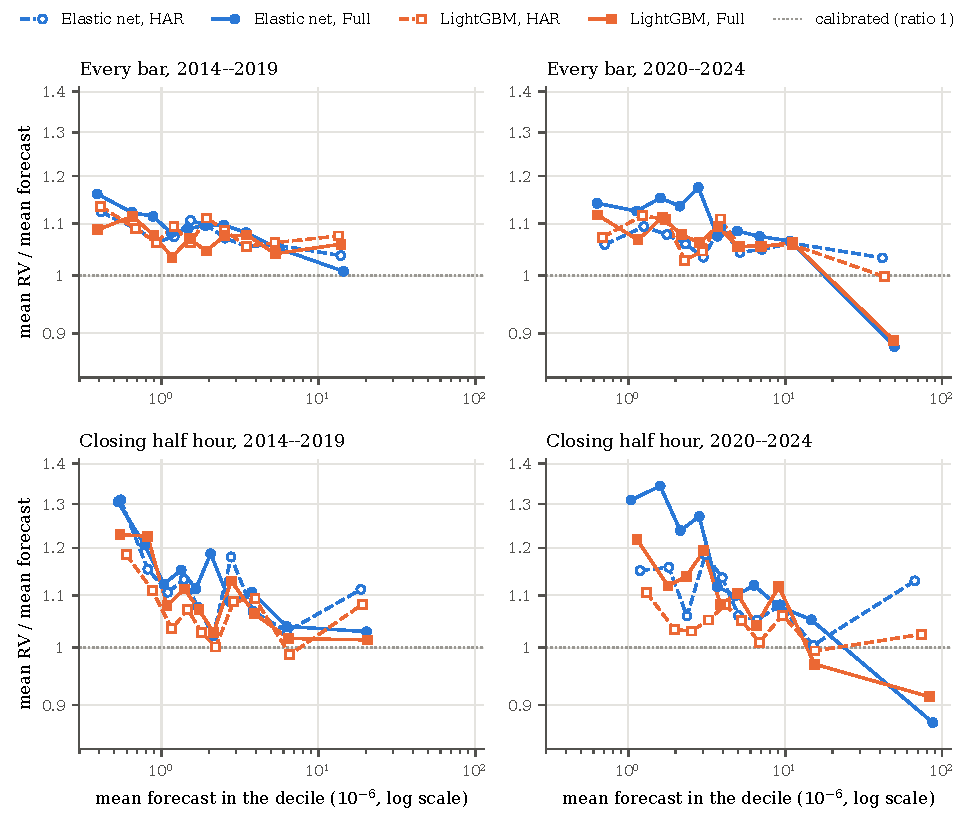
\includegraphics[width=\linewidth]{generated/rehaul_calibration.pdf}
\caption{Calibration by forecast decile. Within each decile of the forecast, the mean realized variance relative to the mean forecast (vertical axis; 1: calibrated, above 1: the forecasts are too low), plotted at the decile's mean forecast (horizontal axis), for the elastic net and LightGBM on the HAR benchmark (open markers, dashed) and on the full predictor set (filled markers, solid); log scales. Top: every bar of Table~\ref{tab:rh_oos}; bottom: the 16:00 bar (the forecast of the closing half hour). Left: \rhcaYearsPre{} ($\rhcaNdaysPre$ days); right: \rhcaYearsOos{} ($\mathcal T_{\mathrm{close}}$, $\rhcaNdaysOos$ days). On every bar in \rhcaYearsOos, the ratio of the full-set elastic net falls from \rhcaBotDecRatioEnetFullBarOos{} in the bottom decile to \rhcaTopDecRatioEnetFullBarOos{} in the top decile (HAR benchmark: \rhcaBotDecRatioEnetHarBarOos{} and \rhcaTopDecRatioEnetHarBarOos), and the top decile carries \rhcaTopDecSeEnetFullBarOos\% of its squared error.}
\label{fig:rh_calibration}
\end{figure}


% ---------------------------------------------------------------------------------------------------------------------
\subsection{Predictor-group ablations: design}
\label{app:rh_results_ablation}
% 2026-10-26 (integration, JFEc): from drafts/2026-10-25_ablations.tex ("Design", "Augmented HAR benchmarks",
% "Late-starting series"); typed counts replaced by \rhdmNSeriesPooled and \rhfiNBuckets, the 3,000-day rule by
% \rhorWindowDays, the "[check]" placeholder on the volatility-demand feed resolved (\rhabLiveVdSpxOcLast), and the
% clause on the HAR-block penalty weight dropped (no macro; Section 5 and Appendix app:rh_hyper state the penalties).
% The draft's result paragraphs are condensed in Section 6 (sec:rh_results_ablation).
\begin{itemize}
\item \textbf{Groups and arms.} The \rhdmNSeriesPooled{} exogenous series form the \rhfiNBuckets{} groups of
  Table~\ref{tab:rh_dm_dictionary}. For each group $g$ we fit two models in every class:
  \begin{itemize}
  \item the full set without $g$ (all of $g$'s trailing averages $u^{(k)}$ and availability shares $\bar a^{(k)}$
    removed), which measures what $g$ contributes given everything else;
  \item the HAR benchmark set with $g$ added, which measures what $g$ contributes on its own.
  \end{itemize}
\item \textbf{Hyperparameters and coverage.} Hyperparameters stay those of the full set: the linear penalties chosen on
  \rhorPenSample{} for the full predictor set, and the single frozen configuration of each tree method. The random
  forest, the most expensive class, is fitted for the \rhfiNBuckets{} additions and for the removal of the realized
  moments. Panel~D of Table~\ref{tab:rh_ablation} restates the full-set row of Table~\ref{tab:rh_oos}.
\item \textbf{Augmented HAR benchmarks.} The first group, the futures' own realized moments, is the natural augmented
  HAR: it adds the return, absolute variation, skewness, quarticity, positive semivariance, bipower variation and
  autocovariance of the same one-minute E-mini returns that define the target. We also fit the three classical
  extensions of the HAR model by OLS, each built from the same one-minute data and passed through the same diurnal
  adjustment, variance-stabilizing transform and trailing averages as every other series; a fourth model adds all
  three.
  \begin{itemize}
  \item The semivariance HAR of \citet{PattonSheppard2015} adds the positive and negative realized semivariances
    $\mathrm{RS}^{\pm}$ of the last half hour; the negative semivariance is $\mathrm{RS}^{-} = \RV - \mathrm{RS}^{+}$,
    exact on every bar of the data.
  \item The HARQ model of \citet{BollerslevPattonQuaedvlieg2016} adds the interaction of the last half hour's realized
    variance with the square root of its realized quarticity $\mathrm{RQ} = (N/3)\sum_k r^4_{t,i,k}$ (in the
    volatility units of the design, $\sqrt{\RV\,\mathrm{RQ}^{1/2}}$).
  \item The leverage HAR of \citet{CorsiReno2012} adds the negative part of the half-hour return, $\min(r_{t,i}, 0)$,
    at every HAR horizon.
  \end{itemize}
\item \textbf{Late-starting series.} The implied-volatility, sentiment and volatility-demand series start after the
  data, and a series enters as zero until the rolling window holds \rhorWindowDays{} trading days of its history
  (Section~\ref{sec:rh_predictors}). In the evaluation span this rule binds for most of the sample:
  \begin{itemize}
  \item the VIX enters on \rhabLiveVixFromKone{} (its longest average on \rhabLiveVixFromKlast), VIX3M on
    \rhabLiveVixthreemFromKone, and VVIX on \rhabLiveVvixFromKone;
  \item StockTwits attention on \rhabLiveAttnFromKone{} and the other StockTwits series on \rhabLiveSentFromKone;
  \item the volatility-demand series on \rhabLiveVdSpxOcFromKone{} (their feed stops on \rhabLiveVdSpxOcLast);
  \item before those dates the groups contribute only their availability shares, so the rows of these groups in
    Panels~A and~B measure the series over the later part of the span only; Panel~E scores them on the bars on which
    their value averages are live.
  \end{itemize}
\end{itemize}

% ---------------------------------------------------------------------------------------------------------------------
% 2026-10-28 (v2 of Sections 6-7, author approved preliminarily; drafts/MAP_06_07.md, open point 4): added -- the day
% split of Sections 6.2 (sec:rh_results_channels) and 7 (sec:rh_fi), its rule and the order of the analyses. Sources:
% results/channels_2026-10-26/RULE.txt (committed in 86ee222 on 26 October 2026, before any day-type scoring of the
% patched forecasts; its DISCLOSURE paragraph is paraphrased in "Order of the analyses", without its exploratory
% numbers) and SUMMARY.md; results/channels_2026-10-26/factor/SUMMARY.md (RULE section 4); the ablation rule
% results/ablations_2014start_w3000/RULE.txt, addenda E (i) (the forest's FOMC removal stopped), F (HAR + RM + FOMC),
% G and I (beyond it; with results/beyond_trees_2026-10-27/RULE.txt). Backing of the words that are not macros: "no
% other split is used for inference" and "every class and every predictor group is reported" = RULE section 0; the
% reading thresholds "three-quarters", "more than one and a half times" and "at most one" = RULE item 3 (design
% constants, in words as in Section 7; no macro holds them); the forest's place in the trees' reading = RULE item 3
% ("the forest where its arms exist") and SUMMARY.md ("left out of the model-type vote"); "reports where each
% definition holds" = the generator's REDUNDANT-first column (SUMMARY.md, item 3 ii; \rhch...NConcTest / NRedTest),
% which is not in the RULE; k = 1, 2, 3, 5, 10, 20 (PCA), 1, 2, 3 (PLS), k <= 3 and R_10 = RULE item 4 design. The
% coordinator's additional comparison against HAR + RM (\rhchX..., not pre-registered) is not reported in the paper.
\subsection{FOMC statement days and ordinary days}
\label{app:rh_channels}
\begin{itemize}
\item \textbf{Day types.} Sections~\ref{sec:rh_results_channels} and~\ref{sec:rh_fi} score the forecasts of
  Table~\ref{tab:rh_oos} separately on two kinds of day. Statement days are the \rhchNEventDays{} days of
  $\mathcal T_{\mathrm{oos}}$ with a scheduled FOMC statement, from the calendar of Appendix~\ref{app:rh_dp_fomc}
  (unscheduled meetings excluded), with \rhchNEventBars{} of the \rhchNBars{} scored bars; ordinary days are the other
  \rhchNOrdDays. The Federal Reserve publishes its meeting calendar in advance, so the type of a day is known before
  every forecast of it. No other split is used for inference; the splits by bar of the day are descriptive. Loss,
  benchmarks and tests are those of Table~\ref{tab:rh_oos}, with the Diebold--Mariano test on the daily average loss
  over the days of the type (Newey--West lag \rhchHacLag{} on both types).
\item \textbf{Order of the analyses.} The day split was introduced after the every-bar results of
  Table~\ref{tab:rh_oos} and of the predictor-group ablations had been seen.
  \begin{itemize}
  \item Before the split was formalized, an exploratory rescoring by day type of the ablation forecasts on the design
    before the FOMC fixes of Appendix~\ref{app:rh_dp_fomc} had shown the pattern reported in
    Sections~\ref{sec:rh_results_channels} and~\ref{sec:rh_fi}: a large share of the every-bar gain on the afternoons
    of the statement days; a gain on ordinary days in which the futures' realized moments are the largest single
    group and the only one whose removal costs much; and the lasso ahead of the ridge and the elastic net on statement
    days but behind them on ordinary days.
  \item A written rule then fixed the day types, the tests, the readings below and their thresholds, and the factor
    test, before any forecast on the fixed design was scored by day type. Every number the paper reports by day type
    comes from the fixed design under that rule; the exploratory numbers are not reported. Every model class and every
    predictor group is reported; none was dropped after scoring.
  \end{itemize}
\item \textbf{Readings} (Table~\ref{tab:rh_channels_abl}). On each day type, with the joint gain that of the full set
  over the HAR benchmark on that day type, the gain is
  \begin{itemize}
  \item concentrated if one group, added alone to the HAR benchmark set, recovers at least three-quarters of the joint
    gain and removing it from the full set raises the loss significantly;
  \item spread across correlated proxies (redundant) if the groups' separate gains sum to more than one and a half
    times the joint gain and removing at most one group raises the loss significantly;
  \item mixed otherwise.
  \end{itemize}
  The penalized linear models are read by the majority of the ridge, lasso and elastic net, the trees by LightGBM and
  XGBoost, with the random forest where its arms exist. The rule applies the two definitions in this order. Both can
  hold, when one group carries the gain and the others repeat its information, so Section~\ref{sec:rh_fi} reports
  where each holds. The three corrections of Table~\ref{tab:rh_channels_corr} agree for a class when they lie within
  \rhchAgreePp{} percentage points of one another; a disagreement is reported, not resolved.
\item \textbf{The factor test} (Table~\ref{tab:rh_factor}, Figure~\ref{fig:rh_factor}). Fixed by the same rule and
  scored primarily on ordinary days: the OLS on the HAR benchmark set plus the first $k$ principal components
  ($k = 1, 2, 3, 5, 10, 20$) or partial-least-squares components ($k = 1, 2, 3$) of the \rhfaNBlock{} value averages
  of the \rhfaNSeries{} exogenous series outside the FOMC group, standardized in each window, the loadings recomputed
  once a trading day and the regression at every bar, on the window of Table~\ref{tab:rh_oos}.
  \begin{itemize}
  \item With $k = 0$ it reproduces the OLS row of Table~\ref{tab:rh_oos} on every bar (largest relative difference
    \rhfaGOneMaxRel). The share $R_k$ of the gain recovered is measured against the lower loss of the full-set ridge
    and elastic net.
  \item Reading: a shared factor if some $k \le 3$ has $R_k \ge \rhfaShareThreshold$ and a loss not significantly
    above the full set's; dense beyond a few factors if $R_{10} < \rhfaDenseThreshold$ and the full set beats the
    ten-component model significantly; intermediate otherwise. On ordinary days it is ``\rhfaReading''.
  \end{itemize}
\item \textbf{Tables and coverage.} Table~\ref{tab:rh_channels_abl} reports every group's change added alone and
  removed, for every class on both day types, with the joint gain and the readings; Table~\ref{tab:rh_channels_sparse}
  the lasso against the ridge and the elastic net and the feature-count ladder by day type;
  Table~\ref{tab:rh_channels_corr} and Figure~\ref{fig:rh_channels} the three corrections and where the gain falls.
  Two gaps are marked in the tables: the random forest is fitted for the additions and for removing the realized
  moments only (Appendix~\ref{app:rh_results_ablation}), and the trees' removals other than that of the FOMC group are
  on the design before the FOMC fixes, against the full set on that design.
\item \textbf{Added after the rule.} Not pre-registered, each requested by the author after the results it follows and
  specified in a dated addendum to the ablation rule, or in a rule of its own, before its forecasts were scored:
  \begin{itemize}
  \item the reference HAR\,+\,RM\,+\,FOMC, the HAR benchmark set with the futures' realized moments and the FOMC
    calendar (Table~\ref{tab:rh_ablation}, Panel~D; Section~\ref{sec:rh_results_beyond}), after the results by day
    type;
  \item the tests beyond that reference (Appendix~\ref{app:rh_results_beyond}), after the results against it.
  \end{itemize}
\end{itemize}
% Share of the full set's ordinary-day gain recovered by k components (writeup/make_rehaul_factor.py; RULE item 4)
% AUTO-GENERATED by writeup/make_rehaul_factor.py -- do not edit; re-run the script.
\ifdefined\rhfaReading\else% AUTO-GENERATED by writeup/make_rehaul_factor.py -- do not edit; re-run the script.
% \rhfa... macros: factor-augmented HAR (diffusion index) on Table 1's design (results/channels_2026-10-26/
% RULE.txt section 4; results/channels_2026-10-26/factor).  Spans: Ord = ORDINARY days (primary), All = every
% bar, Ev = the 81 FOMC statement days.  Models: Pca<k>, Pls<k>, Full (the span's L_full model).
\providecommand{\rhfaPcaOneOrdPct}{}\renewcommand{\rhfaPcaOneOrdPct}{0.08}  % pca1 ordinary: QLIKE change vs OLS-HAR, %
\providecommand{\rhfaPcaOneOrdMsePct}{}\renewcommand{\rhfaPcaOneOrdMsePct}{3.28}  % pca1 ordinary: MSE change vs OLS-HAR, %
\providecommand{\rhfaPcaOneOrdDm}{}\renewcommand{\rhfaPcaOneOrdDm}{0.90}  % pca1 ordinary: DM vs OLS-HAR (QLIKE)
\providecommand{\rhfaPcaOneOrdP}{}\renewcommand{\rhfaPcaOneOrdP}{0.369}  % pca1 ordinary: p
\providecommand{\rhfaPcaOneOrdDmFull}{}\renewcommand{\rhfaPcaOneOrdDmFull}{4.89}  % pca1 ordinary: DM vs the full set (enet)
\providecommand{\rhfaPcaOneOrdPFull}{}\renewcommand{\rhfaPcaOneOrdPFull}{$<$0.001}  % pca1 ordinary: p
\providecommand{\rhfaPcaOneOrdR}{}\renewcommand{\rhfaPcaOneOrdR}{$-$0.02}  % pca1 ordinary: R_k
\providecommand{\rhfaPcaTwoOrdPct}{}\renewcommand{\rhfaPcaTwoOrdPct}{0.06}  % pca2 ordinary: QLIKE change vs OLS-HAR, %
\providecommand{\rhfaPcaTwoOrdMsePct}{}\renewcommand{\rhfaPcaTwoOrdMsePct}{1.85}  % pca2 ordinary: MSE change vs OLS-HAR, %
\providecommand{\rhfaPcaTwoOrdDm}{}\renewcommand{\rhfaPcaTwoOrdDm}{0.32}  % pca2 ordinary: DM vs OLS-HAR (QLIKE)
\providecommand{\rhfaPcaTwoOrdP}{}\renewcommand{\rhfaPcaTwoOrdP}{0.748}  % pca2 ordinary: p
\providecommand{\rhfaPcaTwoOrdDmFull}{}\renewcommand{\rhfaPcaTwoOrdDmFull}{4.86}  % pca2 ordinary: DM vs the full set (enet)
\providecommand{\rhfaPcaTwoOrdPFull}{}\renewcommand{\rhfaPcaTwoOrdPFull}{$<$0.001}  % pca2 ordinary: p
\providecommand{\rhfaPcaTwoOrdR}{}\renewcommand{\rhfaPcaTwoOrdR}{$-$0.02}  % pca2 ordinary: R_k
\providecommand{\rhfaPcaThreeOrdPct}{}\renewcommand{\rhfaPcaThreeOrdPct}{0.45}  % pca3 ordinary: QLIKE change vs OLS-HAR, %
\providecommand{\rhfaPcaThreeOrdMsePct}{}\renewcommand{\rhfaPcaThreeOrdMsePct}{5.76}  % pca3 ordinary: MSE change vs OLS-HAR, %
\providecommand{\rhfaPcaThreeOrdDm}{}\renewcommand{\rhfaPcaThreeOrdDm}{1.44}  % pca3 ordinary: DM vs OLS-HAR (QLIKE)
\providecommand{\rhfaPcaThreeOrdP}{}\renewcommand{\rhfaPcaThreeOrdP}{0.151}  % pca3 ordinary: p
\providecommand{\rhfaPcaThreeOrdDmFull}{}\renewcommand{\rhfaPcaThreeOrdDmFull}{5.33}  % pca3 ordinary: DM vs the full set (enet)
\providecommand{\rhfaPcaThreeOrdPFull}{}\renewcommand{\rhfaPcaThreeOrdPFull}{$<$0.001}  % pca3 ordinary: p
\providecommand{\rhfaPcaThreeOrdR}{}\renewcommand{\rhfaPcaThreeOrdR}{$-$0.11}  % pca3 ordinary: R_k
\providecommand{\rhfaPcaFiveOrdPct}{}\renewcommand{\rhfaPcaFiveOrdPct}{0.93}  % pca5 ordinary: QLIKE change vs OLS-HAR, %
\providecommand{\rhfaPcaFiveOrdMsePct}{}\renewcommand{\rhfaPcaFiveOrdMsePct}{3.77}  % pca5 ordinary: MSE change vs OLS-HAR, %
\providecommand{\rhfaPcaFiveOrdDm}{}\renewcommand{\rhfaPcaFiveOrdDm}{1.85}  % pca5 ordinary: DM vs OLS-HAR (QLIKE)
\providecommand{\rhfaPcaFiveOrdP}{}\renewcommand{\rhfaPcaFiveOrdP}{0.064}  % pca5 ordinary: p
\providecommand{\rhfaPcaFiveOrdDmFull}{}\renewcommand{\rhfaPcaFiveOrdDmFull}{5.94}  % pca5 ordinary: DM vs the full set (enet)
\providecommand{\rhfaPcaFiveOrdPFull}{}\renewcommand{\rhfaPcaFiveOrdPFull}{$<$0.001}  % pca5 ordinary: p
\providecommand{\rhfaPcaFiveOrdR}{}\renewcommand{\rhfaPcaFiveOrdR}{$-$0.23}  % pca5 ordinary: R_k
\providecommand{\rhfaPcaTenOrdPct}{}\renewcommand{\rhfaPcaTenOrdPct}{$-$1.06}  % pca10 ordinary: QLIKE change vs OLS-HAR, %
\providecommand{\rhfaPcaTenOrdMsePct}{}\renewcommand{\rhfaPcaTenOrdMsePct}{21.39}  % pca10 ordinary: MSE change vs OLS-HAR, %
\providecommand{\rhfaPcaTenOrdDm}{}\renewcommand{\rhfaPcaTenOrdDm}{$-$2.19}  % pca10 ordinary: DM vs OLS-HAR (QLIKE)
\providecommand{\rhfaPcaTenOrdP}{}\renewcommand{\rhfaPcaTenOrdP}{0.028}  % pca10 ordinary: p
\providecommand{\rhfaPcaTenOrdDmFull}{}\renewcommand{\rhfaPcaTenOrdDmFull}{4.45}  % pca10 ordinary: DM vs the full set (enet)
\providecommand{\rhfaPcaTenOrdPFull}{}\renewcommand{\rhfaPcaTenOrdPFull}{$<$0.001}  % pca10 ordinary: p
\providecommand{\rhfaPcaTenOrdR}{}\renewcommand{\rhfaPcaTenOrdR}{0.27}  % pca10 ordinary: R_k
\providecommand{\rhfaPcaTwentyOrdPct}{}\renewcommand{\rhfaPcaTwentyOrdPct}{$-$1.09}  % pca20 ordinary: QLIKE change vs OLS-HAR, %
\providecommand{\rhfaPcaTwentyOrdMsePct}{}\renewcommand{\rhfaPcaTwentyOrdMsePct}{45.47}  % pca20 ordinary: MSE change vs OLS-HAR, %
\providecommand{\rhfaPcaTwentyOrdDm}{}\renewcommand{\rhfaPcaTwentyOrdDm}{$-$1.53}  % pca20 ordinary: DM vs OLS-HAR (QLIKE)
\providecommand{\rhfaPcaTwentyOrdP}{}\renewcommand{\rhfaPcaTwentyOrdP}{0.126}  % pca20 ordinary: p
\providecommand{\rhfaPcaTwentyOrdDmFull}{}\renewcommand{\rhfaPcaTwentyOrdDmFull}{3.66}  % pca20 ordinary: DM vs the full set (enet)
\providecommand{\rhfaPcaTwentyOrdPFull}{}\renewcommand{\rhfaPcaTwentyOrdPFull}{$<$0.001}  % pca20 ordinary: p
\providecommand{\rhfaPcaTwentyOrdR}{}\renewcommand{\rhfaPcaTwentyOrdR}{0.27}  % pca20 ordinary: R_k
\providecommand{\rhfaPlsOneOrdPct}{}\renewcommand{\rhfaPlsOneOrdPct}{0.01}  % pls1 ordinary: QLIKE change vs OLS-HAR, %
\providecommand{\rhfaPlsOneOrdMsePct}{}\renewcommand{\rhfaPlsOneOrdMsePct}{14.31}  % pls1 ordinary: MSE change vs OLS-HAR, %
\providecommand{\rhfaPlsOneOrdDm}{}\renewcommand{\rhfaPlsOneOrdDm}{0.05}  % pls1 ordinary: DM vs OLS-HAR (QLIKE)
\providecommand{\rhfaPlsOneOrdP}{}\renewcommand{\rhfaPlsOneOrdP}{0.962}  % pls1 ordinary: p
\providecommand{\rhfaPlsOneOrdDmFull}{}\renewcommand{\rhfaPlsOneOrdDmFull}{4.95}  % pls1 ordinary: DM vs the full set (enet)
\providecommand{\rhfaPlsOneOrdPFull}{}\renewcommand{\rhfaPlsOneOrdPFull}{$<$0.001}  % pls1 ordinary: p
\providecommand{\rhfaPlsOneOrdR}{}\renewcommand{\rhfaPlsOneOrdR}{0.00}  % pls1 ordinary: R_k
\providecommand{\rhfaPlsTwoOrdPct}{}\renewcommand{\rhfaPlsTwoOrdPct}{1.57}  % pls2 ordinary: QLIKE change vs OLS-HAR, %
\providecommand{\rhfaPlsTwoOrdMsePct}{}\renewcommand{\rhfaPlsTwoOrdMsePct}{24.30}  % pls2 ordinary: MSE change vs OLS-HAR, %
\providecommand{\rhfaPlsTwoOrdDm}{}\renewcommand{\rhfaPlsTwoOrdDm}{1.29}  % pls2 ordinary: DM vs OLS-HAR (QLIKE)
\providecommand{\rhfaPlsTwoOrdP}{}\renewcommand{\rhfaPlsTwoOrdP}{0.196}  % pls2 ordinary: p
\providecommand{\rhfaPlsTwoOrdDmFull}{}\renewcommand{\rhfaPlsTwoOrdDmFull}{4.51}  % pls2 ordinary: DM vs the full set (enet)
\providecommand{\rhfaPlsTwoOrdPFull}{}\renewcommand{\rhfaPlsTwoOrdPFull}{$<$0.001}  % pls2 ordinary: p
\providecommand{\rhfaPlsTwoOrdR}{}\renewcommand{\rhfaPlsTwoOrdR}{$-$0.40}  % pls2 ordinary: R_k
\providecommand{\rhfaPlsThreeOrdPct}{}\renewcommand{\rhfaPlsThreeOrdPct}{0.04}  % pls3 ordinary: QLIKE change vs OLS-HAR, %
\providecommand{\rhfaPlsThreeOrdMsePct}{}\renewcommand{\rhfaPlsThreeOrdMsePct}{99.04}  % pls3 ordinary: MSE change vs OLS-HAR, %
\providecommand{\rhfaPlsThreeOrdDm}{}\renewcommand{\rhfaPlsThreeOrdDm}{0.03}  % pls3 ordinary: DM vs OLS-HAR (QLIKE)
\providecommand{\rhfaPlsThreeOrdP}{}\renewcommand{\rhfaPlsThreeOrdP}{0.974}  % pls3 ordinary: p
\providecommand{\rhfaPlsThreeOrdDmFull}{}\renewcommand{\rhfaPlsThreeOrdDmFull}{3.84}  % pls3 ordinary: DM vs the full set (enet)
\providecommand{\rhfaPlsThreeOrdPFull}{}\renewcommand{\rhfaPlsThreeOrdPFull}{$<$0.001}  % pls3 ordinary: p
\providecommand{\rhfaPlsThreeOrdR}{}\renewcommand{\rhfaPlsThreeOrdR}{$-$0.01}  % pls3 ordinary: R_k
\providecommand{\rhfaFullOrdModel}{}\renewcommand{\rhfaFullOrdModel}{elastic net}  % ordinary: L_full model (lower QLIKE of ridge, elastic net)
\providecommand{\rhfaFullOrdPct}{}\renewcommand{\rhfaFullOrdPct}{$-$3.97}  % ordinary: full set QLIKE change vs OLS-HAR, %
\providecommand{\rhfaFullOrdMsePct}{}\renewcommand{\rhfaFullOrdMsePct}{128.86}  % ordinary: full set MSE change vs OLS-HAR, %
\providecommand{\rhfaFullOrdDm}{}\renewcommand{\rhfaFullOrdDm}{$-$4.73}  % ordinary: full set DM vs OLS-HAR
\providecommand{\rhfaFullOrdP}{}\renewcommand{\rhfaFullOrdP}{$<$0.001}  % ordinary: p
\providecommand{\rhfaNOrdDays}{}\renewcommand{\rhfaNOrdDays}{2{,}498}  % ordinary: days
\providecommand{\rhfaNOrdBars}{}\renewcommand{\rhfaNOrdBars}{32{,}474}  % ordinary: bars
\providecommand{\rhfaPcaOneAllPct}{}\renewcommand{\rhfaPcaOneAllPct}{$-$0.05}  % pca1 all: QLIKE change vs OLS-HAR, %
\providecommand{\rhfaPcaOneAllMsePct}{}\renewcommand{\rhfaPcaOneAllMsePct}{3.00}  % pca1 all: MSE change vs OLS-HAR, %
\providecommand{\rhfaPcaOneAllDm}{}\renewcommand{\rhfaPcaOneAllDm}{$-$0.53}  % pca1 all: DM vs OLS-HAR (QLIKE)
\providecommand{\rhfaPcaOneAllP}{}\renewcommand{\rhfaPcaOneAllP}{0.595}  % pca1 all: p
\providecommand{\rhfaPcaOneAllDmFull}{}\renewcommand{\rhfaPcaOneAllDmFull}{7.44}  % pca1 all: DM vs the full set (enet)
\providecommand{\rhfaPcaOneAllPFull}{}\renewcommand{\rhfaPcaOneAllPFull}{$<$0.001}  % pca1 all: p
\providecommand{\rhfaPcaOneAllR}{}\renewcommand{\rhfaPcaOneAllR}{0.01}  % pca1 all: R_k
\providecommand{\rhfaPcaTwoAllPct}{}\renewcommand{\rhfaPcaTwoAllPct}{0.11}  % pca2 all: QLIKE change vs OLS-HAR, %
\providecommand{\rhfaPcaTwoAllMsePct}{}\renewcommand{\rhfaPcaTwoAllMsePct}{1.71}  % pca2 all: MSE change vs OLS-HAR, %
\providecommand{\rhfaPcaTwoAllDm}{}\renewcommand{\rhfaPcaTwoAllDm}{0.55}  % pca2 all: DM vs OLS-HAR (QLIKE)
\providecommand{\rhfaPcaTwoAllP}{}\renewcommand{\rhfaPcaTwoAllP}{0.579}  % pca2 all: p
\providecommand{\rhfaPcaTwoAllDmFull}{}\renewcommand{\rhfaPcaTwoAllDmFull}{7.48}  % pca2 all: DM vs the full set (enet)
\providecommand{\rhfaPcaTwoAllPFull}{}\renewcommand{\rhfaPcaTwoAllPFull}{$<$0.001}  % pca2 all: p
\providecommand{\rhfaPcaTwoAllR}{}\renewcommand{\rhfaPcaTwoAllR}{$-$0.02}  % pca2 all: R_k
\providecommand{\rhfaPcaThreeAllPct}{}\renewcommand{\rhfaPcaThreeAllPct}{0.69}  % pca3 all: QLIKE change vs OLS-HAR, %
\providecommand{\rhfaPcaThreeAllMsePct}{}\renewcommand{\rhfaPcaThreeAllMsePct}{5.30}  % pca3 all: MSE change vs OLS-HAR, %
\providecommand{\rhfaPcaThreeAllDm}{}\renewcommand{\rhfaPcaThreeAllDm}{2.24}  % pca3 all: DM vs OLS-HAR (QLIKE)
\providecommand{\rhfaPcaThreeAllP}{}\renewcommand{\rhfaPcaThreeAllP}{0.025}  % pca3 all: p
\providecommand{\rhfaPcaThreeAllDmFull}{}\renewcommand{\rhfaPcaThreeAllDmFull}{7.96}  % pca3 all: DM vs the full set (enet)
\providecommand{\rhfaPcaThreeAllPFull}{}\renewcommand{\rhfaPcaThreeAllPFull}{$<$0.001}  % pca3 all: p
\providecommand{\rhfaPcaThreeAllR}{}\renewcommand{\rhfaPcaThreeAllR}{$-$0.10}  % pca3 all: R_k
\providecommand{\rhfaPcaFiveAllPct}{}\renewcommand{\rhfaPcaFiveAllPct}{0.94}  % pca5 all: QLIKE change vs OLS-HAR, %
\providecommand{\rhfaPcaFiveAllMsePct}{}\renewcommand{\rhfaPcaFiveAllMsePct}{3.39}  % pca5 all: MSE change vs OLS-HAR, %
\providecommand{\rhfaPcaFiveAllDm}{}\renewcommand{\rhfaPcaFiveAllDm}{2.05}  % pca5 all: DM vs OLS-HAR (QLIKE)
\providecommand{\rhfaPcaFiveAllP}{}\renewcommand{\rhfaPcaFiveAllP}{0.041}  % pca5 all: p
\providecommand{\rhfaPcaFiveAllDmFull}{}\renewcommand{\rhfaPcaFiveAllDmFull}{8.48}  % pca5 all: DM vs the full set (enet)
\providecommand{\rhfaPcaFiveAllPFull}{}\renewcommand{\rhfaPcaFiveAllPFull}{$<$0.001}  % pca5 all: p
\providecommand{\rhfaPcaFiveAllR}{}\renewcommand{\rhfaPcaFiveAllR}{$-$0.14}  % pca5 all: R_k
\providecommand{\rhfaPcaTenAllPct}{}\renewcommand{\rhfaPcaTenAllPct}{$-$0.66}  % pca10 all: QLIKE change vs OLS-HAR, %
\providecommand{\rhfaPcaTenAllMsePct}{}\renewcommand{\rhfaPcaTenAllMsePct}{19.64}  % pca10 all: MSE change vs OLS-HAR, %
\providecommand{\rhfaPcaTenAllDm}{}\renewcommand{\rhfaPcaTenAllDm}{$-$1.43}  % pca10 all: DM vs OLS-HAR (QLIKE)
\providecommand{\rhfaPcaTenAllP}{}\renewcommand{\rhfaPcaTenAllP}{0.152}  % pca10 all: p
\providecommand{\rhfaPcaTenAllDmFull}{}\renewcommand{\rhfaPcaTenAllDmFull}{7.31}  % pca10 all: DM vs the full set (enet)
\providecommand{\rhfaPcaTenAllPFull}{}\renewcommand{\rhfaPcaTenAllPFull}{$<$0.001}  % pca10 all: p
\providecommand{\rhfaPcaTenAllR}{}\renewcommand{\rhfaPcaTenAllR}{0.10}  % pca10 all: R_k
\providecommand{\rhfaPcaTwentyAllPct}{}\renewcommand{\rhfaPcaTwentyAllPct}{$-$0.87}  % pca20 all: QLIKE change vs OLS-HAR, %
\providecommand{\rhfaPcaTwentyAllMsePct}{}\renewcommand{\rhfaPcaTwentyAllMsePct}{41.73}  % pca20 all: MSE change vs OLS-HAR, %
\providecommand{\rhfaPcaTwentyAllDm}{}\renewcommand{\rhfaPcaTwentyAllDm}{$-$1.28}  % pca20 all: DM vs OLS-HAR (QLIKE)
\providecommand{\rhfaPcaTwentyAllP}{}\renewcommand{\rhfaPcaTwentyAllP}{0.201}  % pca20 all: p
\providecommand{\rhfaPcaTwentyAllDmFull}{}\renewcommand{\rhfaPcaTwentyAllDmFull}{6.40}  % pca20 all: DM vs the full set (enet)
\providecommand{\rhfaPcaTwentyAllPFull}{}\renewcommand{\rhfaPcaTwentyAllPFull}{$<$0.001}  % pca20 all: p
\providecommand{\rhfaPcaTwentyAllR}{}\renewcommand{\rhfaPcaTwentyAllR}{0.13}  % pca20 all: R_k
\providecommand{\rhfaPlsOneAllPct}{}\renewcommand{\rhfaPlsOneAllPct}{$-$0.23}  % pls1 all: QLIKE change vs OLS-HAR, %
\providecommand{\rhfaPlsOneAllMsePct}{}\renewcommand{\rhfaPlsOneAllMsePct}{13.12}  % pls1 all: MSE change vs OLS-HAR, %
\providecommand{\rhfaPlsOneAllDm}{}\renewcommand{\rhfaPlsOneAllDm}{$-$1.07}  % pls1 all: DM vs OLS-HAR (QLIKE)
\providecommand{\rhfaPlsOneAllP}{}\renewcommand{\rhfaPlsOneAllP}{0.284}  % pls1 all: p
\providecommand{\rhfaPlsOneAllDmFull}{}\renewcommand{\rhfaPlsOneAllDmFull}{7.49}  % pls1 all: DM vs the full set (enet)
\providecommand{\rhfaPlsOneAllPFull}{}\renewcommand{\rhfaPlsOneAllPFull}{$<$0.001}  % pls1 all: p
\providecommand{\rhfaPlsOneAllR}{}\renewcommand{\rhfaPlsOneAllR}{0.03}  % pls1 all: R_k
\providecommand{\rhfaPlsTwoAllPct}{}\renewcommand{\rhfaPlsTwoAllPct}{1.66}  % pls2 all: QLIKE change vs OLS-HAR, %
\providecommand{\rhfaPlsTwoAllMsePct}{}\renewcommand{\rhfaPlsTwoAllMsePct}{22.30}  % pls2 all: MSE change vs OLS-HAR, %
\providecommand{\rhfaPlsTwoAllDm}{}\renewcommand{\rhfaPlsTwoAllDm}{1.55}  % pls2 all: DM vs OLS-HAR (QLIKE)
\providecommand{\rhfaPlsTwoAllP}{}\renewcommand{\rhfaPlsTwoAllP}{0.120}  % pls2 all: p
\providecommand{\rhfaPlsTwoAllDmFull}{}\renewcommand{\rhfaPlsTwoAllDmFull}{6.99}  % pls2 all: DM vs the full set (enet)
\providecommand{\rhfaPlsTwoAllPFull}{}\renewcommand{\rhfaPlsTwoAllPFull}{$<$0.001}  % pls2 all: p
\providecommand{\rhfaPlsTwoAllR}{}\renewcommand{\rhfaPlsTwoAllR}{$-$0.25}  % pls2 all: R_k
\providecommand{\rhfaPlsThreeAllPct}{}\renewcommand{\rhfaPlsThreeAllPct}{0.01}  % pls3 all: QLIKE change vs OLS-HAR, %
\providecommand{\rhfaPlsThreeAllMsePct}{}\renewcommand{\rhfaPlsThreeAllMsePct}{90.89}  % pls3 all: MSE change vs OLS-HAR, %
\providecommand{\rhfaPlsThreeAllDm}{}\renewcommand{\rhfaPlsThreeAllDm}{0.01}  % pls3 all: DM vs OLS-HAR (QLIKE)
\providecommand{\rhfaPlsThreeAllP}{}\renewcommand{\rhfaPlsThreeAllP}{0.989}  % pls3 all: p
\providecommand{\rhfaPlsThreeAllDmFull}{}\renewcommand{\rhfaPlsThreeAllDmFull}{6.39}  % pls3 all: DM vs the full set (enet)
\providecommand{\rhfaPlsThreeAllPFull}{}\renewcommand{\rhfaPlsThreeAllPFull}{$<$0.001}  % pls3 all: p
\providecommand{\rhfaPlsThreeAllR}{}\renewcommand{\rhfaPlsThreeAllR}{0.00}  % pls3 all: R_k
\providecommand{\rhfaFullAllModel}{}\renewcommand{\rhfaFullAllModel}{elastic net}  % all: L_full model (lower QLIKE of ridge, elastic net)
\providecommand{\rhfaFullAllPct}{}\renewcommand{\rhfaFullAllPct}{$-$6.69}  % all: full set QLIKE change vs OLS-HAR, %
\providecommand{\rhfaFullAllMsePct}{}\renewcommand{\rhfaFullAllMsePct}{117.67}  % all: full set MSE change vs OLS-HAR, %
\providecommand{\rhfaFullAllDm}{}\renewcommand{\rhfaFullAllDm}{$-$7.36}  % all: full set DM vs OLS-HAR
\providecommand{\rhfaFullAllP}{}\renewcommand{\rhfaFullAllP}{$<$0.001}  % all: p
\providecommand{\rhfaNAllDays}{}\renewcommand{\rhfaNAllDays}{2{,}579}  % all: days
\providecommand{\rhfaNAllBars}{}\renewcommand{\rhfaNAllBars}{33{,}527}  % all: bars
\providecommand{\rhfaPcaOneEvPct}{}\renewcommand{\rhfaPcaOneEvPct}{$-$0.82}  % pca1 event: QLIKE change vs OLS-HAR, %
\providecommand{\rhfaPcaOneEvMsePct}{}\renewcommand{\rhfaPcaOneEvMsePct}{$-$0.06}  % pca1 event: MSE change vs OLS-HAR, %
\providecommand{\rhfaPcaOneEvDm}{}\renewcommand{\rhfaPcaOneEvDm}{$-$1.95}  % pca1 event: DM vs OLS-HAR (QLIKE)
\providecommand{\rhfaPcaOneEvP}{}\renewcommand{\rhfaPcaOneEvP}{0.051}  % pca1 event: p
\providecommand{\rhfaPcaOneEvDmFull}{}\renewcommand{\rhfaPcaOneEvDmFull}{6.60}  % pca1 event: DM vs the full set (enet)
\providecommand{\rhfaPcaOneEvPFull}{}\renewcommand{\rhfaPcaOneEvPFull}{$<$0.001}  % pca1 event: p
\providecommand{\rhfaPcaOneEvR}{}\renewcommand{\rhfaPcaOneEvR}{0.04}  % pca1 event: R_k
\providecommand{\rhfaPcaTwoEvPct}{}\renewcommand{\rhfaPcaTwoEvPct}{0.39}  % pca2 event: QLIKE change vs OLS-HAR, %
\providecommand{\rhfaPcaTwoEvMsePct}{}\renewcommand{\rhfaPcaTwoEvMsePct}{0.12}  % pca2 event: MSE change vs OLS-HAR, %
\providecommand{\rhfaPcaTwoEvDm}{}\renewcommand{\rhfaPcaTwoEvDm}{0.36}  % pca2 event: DM vs OLS-HAR (QLIKE)
\providecommand{\rhfaPcaTwoEvP}{}\renewcommand{\rhfaPcaTwoEvP}{0.715}  % pca2 event: p
\providecommand{\rhfaPcaTwoEvDmFull}{}\renewcommand{\rhfaPcaTwoEvDmFull}{6.20}  % pca2 event: DM vs the full set (enet)
\providecommand{\rhfaPcaTwoEvPFull}{}\renewcommand{\rhfaPcaTwoEvPFull}{$<$0.001}  % pca2 event: p
\providecommand{\rhfaPcaTwoEvR}{}\renewcommand{\rhfaPcaTwoEvR}{$-$0.02}  % pca2 event: R_k
\providecommand{\rhfaPcaThreeEvPct}{}\renewcommand{\rhfaPcaThreeEvPct}{2.06}  % pca3 event: QLIKE change vs OLS-HAR, %
\providecommand{\rhfaPcaThreeEvMsePct}{}\renewcommand{\rhfaPcaThreeEvMsePct}{0.11}  % pca3 event: MSE change vs OLS-HAR, %
\providecommand{\rhfaPcaThreeEvDm}{}\renewcommand{\rhfaPcaThreeEvDm}{2.48}  % pca3 event: DM vs OLS-HAR (QLIKE)
\providecommand{\rhfaPcaThreeEvP}{}\renewcommand{\rhfaPcaThreeEvP}{0.013}  % pca3 event: p
\providecommand{\rhfaPcaThreeEvDmFull}{}\renewcommand{\rhfaPcaThreeEvDmFull}{6.74}  % pca3 event: DM vs the full set (enet)
\providecommand{\rhfaPcaThreeEvPFull}{}\renewcommand{\rhfaPcaThreeEvPFull}{$<$0.001}  % pca3 event: p
\providecommand{\rhfaPcaThreeEvR}{}\renewcommand{\rhfaPcaThreeEvR}{$-$0.09}  % pca3 event: R_k
\providecommand{\rhfaPcaFiveEvPct}{}\renewcommand{\rhfaPcaFiveEvPct}{1.05}  % pca5 event: QLIKE change vs OLS-HAR, %
\providecommand{\rhfaPcaFiveEvMsePct}{}\renewcommand{\rhfaPcaFiveEvMsePct}{$-$0.86}  % pca5 event: MSE change vs OLS-HAR, %
\providecommand{\rhfaPcaFiveEvDm}{}\renewcommand{\rhfaPcaFiveEvDm}{0.75}  % pca5 event: DM vs OLS-HAR (QLIKE)
\providecommand{\rhfaPcaFiveEvP}{}\renewcommand{\rhfaPcaFiveEvP}{0.453}  % pca5 event: p
\providecommand{\rhfaPcaFiveEvDmFull}{}\renewcommand{\rhfaPcaFiveEvDmFull}{6.70}  % pca5 event: DM vs the full set (enet)
\providecommand{\rhfaPcaFiveEvPFull}{}\renewcommand{\rhfaPcaFiveEvPFull}{$<$0.001}  % pca5 event: p
\providecommand{\rhfaPcaFiveEvR}{}\renewcommand{\rhfaPcaFiveEvR}{$-$0.05}  % pca5 event: R_k
\providecommand{\rhfaPcaTenEvPct}{}\renewcommand{\rhfaPcaTenEvPct}{1.72}  % pca10 event: QLIKE change vs OLS-HAR, %
\providecommand{\rhfaPcaTenEvMsePct}{}\renewcommand{\rhfaPcaTenEvMsePct}{$-$0.07}  % pca10 event: MSE change vs OLS-HAR, %
\providecommand{\rhfaPcaTenEvDm}{}\renewcommand{\rhfaPcaTenEvDm}{1.03}  % pca10 event: DM vs OLS-HAR (QLIKE)
\providecommand{\rhfaPcaTenEvP}{}\renewcommand{\rhfaPcaTenEvP}{0.302}  % pca10 event: p
\providecommand{\rhfaPcaTenEvDmFull}{}\renewcommand{\rhfaPcaTenEvDmFull}{5.52}  % pca10 event: DM vs the full set (enet)
\providecommand{\rhfaPcaTenEvPFull}{}\renewcommand{\rhfaPcaTenEvPFull}{$<$0.001}  % pca10 event: p
\providecommand{\rhfaPcaTenEvR}{}\renewcommand{\rhfaPcaTenEvR}{$-$0.08}  % pca10 event: R_k
\providecommand{\rhfaPcaTwentyEvPct}{}\renewcommand{\rhfaPcaTwentyEvPct}{0.39}  % pca20 event: QLIKE change vs OLS-HAR, %
\providecommand{\rhfaPcaTwentyEvMsePct}{}\renewcommand{\rhfaPcaTwentyEvMsePct}{$-$0.48}  % pca20 event: MSE change vs OLS-HAR, %
\providecommand{\rhfaPcaTwentyEvDm}{}\renewcommand{\rhfaPcaTwentyEvDm}{0.30}  % pca20 event: DM vs OLS-HAR (QLIKE)
\providecommand{\rhfaPcaTwentyEvP}{}\renewcommand{\rhfaPcaTwentyEvP}{0.762}  % pca20 event: p
\providecommand{\rhfaPcaTwentyEvDmFull}{}\renewcommand{\rhfaPcaTwentyEvDmFull}{5.91}  % pca20 event: DM vs the full set (enet)
\providecommand{\rhfaPcaTwentyEvPFull}{}\renewcommand{\rhfaPcaTwentyEvPFull}{$<$0.001}  % pca20 event: p
\providecommand{\rhfaPcaTwentyEvR}{}\renewcommand{\rhfaPcaTwentyEvR}{$-$0.02}  % pca20 event: R_k
\providecommand{\rhfaPlsOneEvPct}{}\renewcommand{\rhfaPlsOneEvPct}{$-$1.66}  % pls1 event: QLIKE change vs OLS-HAR, %
\providecommand{\rhfaPlsOneEvMsePct}{}\renewcommand{\rhfaPlsOneEvMsePct}{$-$0.32}  % pls1 event: MSE change vs OLS-HAR, %
\providecommand{\rhfaPlsOneEvDm}{}\renewcommand{\rhfaPlsOneEvDm}{$-$2.59}  % pls1 event: DM vs OLS-HAR (QLIKE)
\providecommand{\rhfaPlsOneEvP}{}\renewcommand{\rhfaPlsOneEvP}{0.010}  % pls1 event: p
\providecommand{\rhfaPlsOneEvDmFull}{}\renewcommand{\rhfaPlsOneEvDmFull}{6.61}  % pls1 event: DM vs the full set (enet)
\providecommand{\rhfaPlsOneEvPFull}{}\renewcommand{\rhfaPlsOneEvPFull}{$<$0.001}  % pls1 event: p
\providecommand{\rhfaPlsOneEvR}{}\renewcommand{\rhfaPlsOneEvR}{0.07}  % pls1 event: R_k
\providecommand{\rhfaPlsTwoEvPct}{}\renewcommand{\rhfaPlsTwoEvPct}{2.22}  % pls2 event: QLIKE change vs OLS-HAR, %
\providecommand{\rhfaPlsTwoEvMsePct}{}\renewcommand{\rhfaPlsTwoEvMsePct}{$-$0.33}  % pls2 event: MSE change vs OLS-HAR, %
\providecommand{\rhfaPlsTwoEvDm}{}\renewcommand{\rhfaPlsTwoEvDm}{1.79}  % pls2 event: DM vs OLS-HAR (QLIKE)
\providecommand{\rhfaPlsTwoEvP}{}\renewcommand{\rhfaPlsTwoEvP}{0.074}  % pls2 event: p
\providecommand{\rhfaPlsTwoEvDmFull}{}\renewcommand{\rhfaPlsTwoEvDmFull}{6.63}  % pls2 event: DM vs the full set (enet)
\providecommand{\rhfaPlsTwoEvPFull}{}\renewcommand{\rhfaPlsTwoEvPFull}{$<$0.001}  % pls2 event: p
\providecommand{\rhfaPlsTwoEvR}{}\renewcommand{\rhfaPlsTwoEvR}{$-$0.10}  % pls2 event: R_k
\providecommand{\rhfaPlsThreeEvPct}{}\renewcommand{\rhfaPlsThreeEvPct}{$-$0.12}  % pls3 event: QLIKE change vs OLS-HAR, %
\providecommand{\rhfaPlsThreeEvMsePct}{}\renewcommand{\rhfaPlsThreeEvMsePct}{$-$1.07}  % pls3 event: MSE change vs OLS-HAR, %
\providecommand{\rhfaPlsThreeEvDm}{}\renewcommand{\rhfaPlsThreeEvDm}{$-$0.06}  % pls3 event: DM vs OLS-HAR (QLIKE)
\providecommand{\rhfaPlsThreeEvP}{}\renewcommand{\rhfaPlsThreeEvP}{0.949}  % pls3 event: p
\providecommand{\rhfaPlsThreeEvDmFull}{}\renewcommand{\rhfaPlsThreeEvDmFull}{5.29}  % pls3 event: DM vs the full set (enet)
\providecommand{\rhfaPlsThreeEvPFull}{}\renewcommand{\rhfaPlsThreeEvPFull}{$<$0.001}  % pls3 event: p
\providecommand{\rhfaPlsThreeEvR}{}\renewcommand{\rhfaPlsThreeEvR}{0.01}  % pls3 event: R_k
\providecommand{\rhfaFullEvModel}{}\renewcommand{\rhfaFullEvModel}{elastic net}  % event: L_full model (lower QLIKE of ridge, elastic net)
\providecommand{\rhfaFullEvPct}{}\renewcommand{\rhfaFullEvPct}{$-$22.61}  % event: full set QLIKE change vs OLS-HAR, %
\providecommand{\rhfaFullEvMsePct}{}\renewcommand{\rhfaFullEvMsePct}{$-$8.54}  % event: full set MSE change vs OLS-HAR, %
\providecommand{\rhfaFullEvDm}{}\renewcommand{\rhfaFullEvDm}{$-$6.79}  % event: full set DM vs OLS-HAR
\providecommand{\rhfaFullEvP}{}\renewcommand{\rhfaFullEvP}{$<$0.001}  % event: p
\providecommand{\rhfaNEvDays}{}\renewcommand{\rhfaNEvDays}{81}  % event: days
\providecommand{\rhfaNEvBars}{}\renewcommand{\rhfaNEvBars}{1{,}053}  % event: bars
\providecommand{\rhfaReading}{}\renewcommand{\rhfaReading}{dense beyond a few factors}  % the RULE's reading, ORDINARY days
\providecommand{\rhfaBestSmall}{}\renewcommand{\rhfaBestSmall}{PLS, $k = 1$}  % the k <= 3 model with the highest R_k on ORDINARY days
\providecommand{\rhfaBestSmallR}{}\renewcommand{\rhfaBestSmallR}{0.00}  % its R_k
\providecommand{\rhfaBestSmallPFull}{}\renewcommand{\rhfaBestSmallPFull}{$<$0.001}  % its DM p against the full set
\providecommand{\rhfaNSharedModels}{}\renewcommand{\rhfaNSharedModels}{0}  % k <= 3 models meeting the SHARED FACTOR condition
\providecommand{\rhfaShareThreshold}{}\renewcommand{\rhfaShareThreshold}{0.75}  % SHARED FACTOR: R_k threshold
\providecommand{\rhfaDenseThreshold}{}\renewcommand{\rhfaDenseThreshold}{0.5}  % DENSE: R_10 threshold
\providecommand{\rhfaNBlock}{}\renewcommand{\rhfaNBlock}{258}  % block columns (value averages, 43 series x 6 horizons)
\providecommand{\rhfaNSeries}{}\renewcommand{\rhfaNSeries}{43}  % non-FOMC exogenous series
\providecommand{\rhfaNActiveMin}{}\renewcommand{\rhfaNActiveMin}{198}  % fewest active block columns on a scored day
\providecommand{\rhfaNActiveMax}{}\renewcommand{\rhfaNActiveMax}{257}  % most active block columns on a scored day
\providecommand{\rhfaSharePcOne}{}\renewcommand{\rhfaSharePcOne}{26.3}  % mean share of block variance, component 1, %
\providecommand{\rhfaSharePcTwo}{}\renewcommand{\rhfaSharePcTwo}{9.7}  % mean share of block variance, component 2, %
\providecommand{\rhfaSharePcThree}{}\renewcommand{\rhfaSharePcThree}{7.6}  % mean share of block variance, component 3, %
\providecommand{\rhfaShareCumOne}{}\renewcommand{\rhfaShareCumOne}{26.3}  % mean share in components 1-1, %
\providecommand{\rhfaShareCumTwo}{}\renewcommand{\rhfaShareCumTwo}{36.0}  % mean share in components 1-2, %
\providecommand{\rhfaShareCumThree}{}\renewcommand{\rhfaShareCumThree}{43.6}  % mean share in components 1-3, %
\providecommand{\rhfaShareCumFive}{}\renewcommand{\rhfaShareCumFive}{52.6}  % mean share in components 1-5, %
\providecommand{\rhfaShareCumTen}{}\renewcommand{\rhfaShareCumTen}{66.2}  % mean share in components 1-10, %
\providecommand{\rhfaShareCumTwenty}{}\renewcommand{\rhfaShareCumTwenty}{78.8}  % mean share in components 1-20, %
\providecommand{\rhfaShareCumThreeMin}{}\renewcommand{\rhfaShareCumThreeMin}{36.6}  % components 1-3: lowest day, %
\providecommand{\rhfaShareCumThreeMax}{}\renewcommand{\rhfaShareCumThreeMax}{47.1}  % components 1-3: highest day, %
\providecommand{\rhfaLoadRm}{}\renewcommand{\rhfaLoadRm}{2.61}  % PC1: sum of |loadings|, Realized moments
\providecommand{\rhfaLoadSqRm}{}\renewcommand{\rhfaLoadSqRm}{22.3}  % PC1: share of squared loadings, Realized moments, %
\providecommand{\rhfaPlsLoadRm}{}\renewcommand{\rhfaPlsLoadRm}{3.04}  % PLS1: sum of |weights|, Realized moments
\providecommand{\rhfaPlsLoadSqRm}{}\renewcommand{\rhfaPlsLoadSqRm}{34.0}  % PLS1: share of squared weights, Realized moments, %
\providecommand{\rhfaNColsRm}{}\renewcommand{\rhfaNColsRm}{42.0}  % active block columns of Realized moments (mean over days)
\providecommand{\rhfaLoadLiq}{}\renewcommand{\rhfaLoadLiq}{3.84}  % PC1: sum of |loadings|, Liquidity
\providecommand{\rhfaLoadSqLiq}{}\renewcommand{\rhfaLoadSqLiq}{21.2}  % PC1: share of squared loadings, Liquidity, %
\providecommand{\rhfaPlsLoadLiq}{}\renewcommand{\rhfaPlsLoadLiq}{3.95}  % PLS1: sum of |weights|, Liquidity
\providecommand{\rhfaPlsLoadSqLiq}{}\renewcommand{\rhfaPlsLoadSqLiq}{26.8}  % PLS1: share of squared weights, Liquidity, %
\providecommand{\rhfaNColsLiq}{}\renewcommand{\rhfaNColsLiq}{84.0}  % active block columns of Liquidity (mean over days)
\providecommand{\rhfaLoadEw}{}\renewcommand{\rhfaLoadEw}{2.97}  % PC1: sum of |loadings|, Equal-weighted market
\providecommand{\rhfaLoadSqEw}{}\renewcommand{\rhfaLoadSqEw}{28.2}  % PC1: share of squared loadings, Equal-weighted market, %
\providecommand{\rhfaPlsLoadEw}{}\renewcommand{\rhfaPlsLoadEw}{2.08}  % PLS1: sum of |weights|, Equal-weighted market
\providecommand{\rhfaPlsLoadSqEw}{}\renewcommand{\rhfaPlsLoadSqEw}{17.7}  % PLS1: share of squared weights, Equal-weighted market, %
\providecommand{\rhfaNColsEw}{}\renewcommand{\rhfaNColsEw}{36.0}  % active block columns of Equal-weighted market (mean over days)
\providecommand{\rhfaLoadVw}{}\renewcommand{\rhfaLoadVw}{2.91}  % PC1: sum of |loadings|, Value-weighted market
\providecommand{\rhfaLoadSqVw}{}\renewcommand{\rhfaLoadSqVw}{27.2}  % PC1: share of squared loadings, Value-weighted market, %
\providecommand{\rhfaPlsLoadVw}{}\renewcommand{\rhfaPlsLoadVw}{2.31}  % PLS1: sum of |weights|, Value-weighted market
\providecommand{\rhfaPlsLoadSqVw}{}\renewcommand{\rhfaPlsLoadSqVw}{21.2}  % PLS1: share of squared weights, Value-weighted market, %
\providecommand{\rhfaNColsVw}{}\renewcommand{\rhfaNColsVw}{36.0}  % active block columns of Value-weighted market (mean over days)
\providecommand{\rhfaLoadSent}{}\renewcommand{\rhfaLoadSent}{0.02}  % PC1: sum of |loadings|, Sentiment
\providecommand{\rhfaLoadSqSent}{}\renewcommand{\rhfaLoadSqSent}{0.0}  % PC1: share of squared loadings, Sentiment, %
\providecommand{\rhfaPlsLoadSent}{}\renewcommand{\rhfaPlsLoadSent}{0.04}  % PLS1: sum of |weights|, Sentiment
\providecommand{\rhfaPlsLoadSqSent}{}\renewcommand{\rhfaPlsLoadSqSent}{0.1}  % PLS1: share of squared weights, Sentiment, %
\providecommand{\rhfaNColsSent}{}\renewcommand{\rhfaNColsSent}{4.0}  % active block columns of Sentiment (mean over days)
\providecommand{\rhfaLoadIv}{}\renewcommand{\rhfaLoadIv}{0.18}  % PC1: sum of |loadings|, Implied volatility
\providecommand{\rhfaLoadSqIv}{}\renewcommand{\rhfaLoadSqIv}{1.1}  % PC1: share of squared loadings, Implied volatility, %
\providecommand{\rhfaPlsLoadIv}{}\renewcommand{\rhfaPlsLoadIv}{0.09}  % PLS1: sum of |weights|, Implied volatility
\providecommand{\rhfaPlsLoadSqIv}{}\renewcommand{\rhfaPlsLoadSqIv}{0.2}  % PLS1: share of squared weights, Implied volatility, %
\providecommand{\rhfaNColsIv}{}\renewcommand{\rhfaNColsIv}{5.1}  % active block columns of Implied volatility (mean over days)
\providecommand{\rhfaLoadVd}{}\renewcommand{\rhfaLoadVd}{0.01}  % PC1: sum of |loadings|, Volatility demand
\providecommand{\rhfaLoadSqVd}{}\renewcommand{\rhfaLoadSqVd}{0.0}  % PC1: share of squared loadings, Volatility demand, %
\providecommand{\rhfaPlsLoadVd}{}\renewcommand{\rhfaPlsLoadVd}{0.01}  % PLS1: sum of |weights|, Volatility demand
\providecommand{\rhfaPlsLoadSqVd}{}\renewcommand{\rhfaPlsLoadSqVd}{0.0}  % PLS1: share of squared weights, Volatility demand, %
\providecommand{\rhfaNColsVd}{}\renewcommand{\rhfaNColsVd}{3.1}  % active block columns of Volatility demand (mean over days)
\providecommand{\rhfaLoadTopGroup}{}\renewcommand{\rhfaLoadTopGroup}{equal-weighted market}  % group with the largest PC1 share of squared loadings
\providecommand{\rhfaGOneMaxRel}{}\renewcommand{\rhfaGOneMaxRel}{$4 \times 10^{-14}$}  % G1: k = 0 vs Table 1's OLS-HAR, max relative difference
\providecommand{\rhfaGTwoMaxRel}{}\renewcommand{\rhfaGTwoMaxRel}{$4 \times 10^{-14}$}  % G2: Gram route vs direct lstsq, max relative difference
\providecommand{\rhfaGTwoNDays}{}\renewcommand{\rhfaGTwoNDays}{7}  % G2 days
\providecommand{\rhfaSdReading}{}\renewcommand{\rhfaSdReading}{dense beyond a few factors}  % sensitivity (s.d.-only entry rule): reading
\providecommand{\rhfaSdPcaOneOrdR}{}\renewcommand{\rhfaSdPcaOneOrdR}{$-$0.02}  % sensitivity: pca1 R_k, ORDINARY days
\providecommand{\rhfaSdPcaTwoOrdR}{}\renewcommand{\rhfaSdPcaTwoOrdR}{$-$0.03}  % sensitivity: pca2 R_k, ORDINARY days
\providecommand{\rhfaSdPcaThreeOrdR}{}\renewcommand{\rhfaSdPcaThreeOrdR}{$-$0.14}  % sensitivity: pca3 R_k, ORDINARY days
\providecommand{\rhfaSdPlsOneOrdR}{}\renewcommand{\rhfaSdPlsOneOrdR}{0.00}  % sensitivity: pls1 R_k, ORDINARY days
\providecommand{\rhfaSdPlsTwoOrdR}{}\renewcommand{\rhfaSdPlsTwoOrdR}{$-$0.40}  % sensitivity: pls2 R_k, ORDINARY days
\providecommand{\rhfaSdPlsThreeOrdR}{}\renewcommand{\rhfaSdPlsThreeOrdR}{$-$0.04}  % sensitivity: pls3 R_k, ORDINARY days
\providecommand{\rhfaSdPcaTenOrdR}{}\renewcommand{\rhfaSdPcaTenOrdR}{0.21}  % sensitivity: pca10 R_k, ORDINARY days
\fi
\begin{figure}[tbp]
\centering
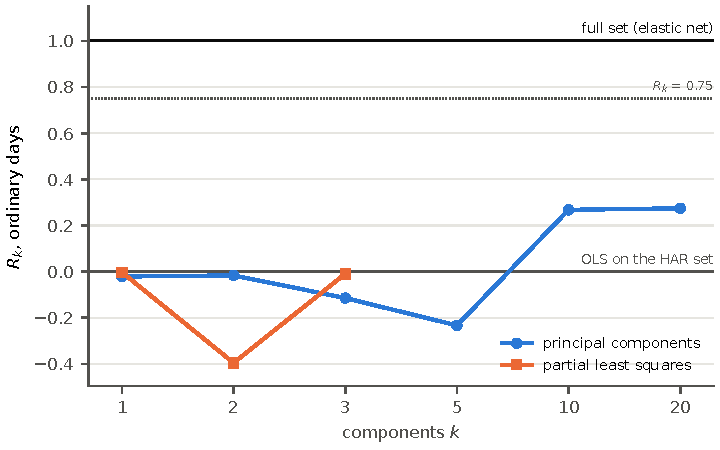
\includegraphics[width=0.75\linewidth]{figures/rehaul_factor_recovery.pdf}
\caption{Share of the full set's ordinary-day gain recovered by $k$ components: $R_k = (L_{\mathrm{HAR}} - L_k)/(L_{\mathrm{HAR}} - L_{\mathrm{full}})$ on the \rhfaNOrdDays{} ordinary days (QLIKE), for OLS on the HAR set plus the first $k$ principal components (blue) or partial least squares components (orange) of the \rhfaNBlock{} non-FOMC value averages. $R_k = 1$: the full set (Table~\ref{tab:rh_oos}'s \rhfaFullOrdModel{}); $R_k = 0$: the OLS on the HAR set. Dotted: $R_k = \rhfaShareThreshold$. Reading: \rhfaReading{} (Table~\ref{tab:rh_factor}).}
\label{fig:rh_factor}
\end{figure}


% ---------------------------------------------------------------------------------------------------------------------
\subsection{Predictor-group ablations: beyond HAR, realized moments and the FOMC calendar}
\label{app:rh_results_beyond}
% 2026-10-27 (coordinator, author request): the follow-up tests beyond HAR + RM + FOMC, cited from Section 6.2
% (sec:rh_results_ablation, "What remains"). Rules: results/ablations_2014start_w3000/RULE.txt addendum G
% (tab:rh_ablation_beyond) and results/beyond_trees_2026-10-27/RULE.txt sections 1-2 (tab:rh_beyond_factor,
% tab:rh_beyond_ladder), each written before its runs were scored. Backing of the words that are not macros:
% "each remaining group ... lowers": \rhab{Lgbm,Xgb}AddRmFomc{Ew,Vw,Liq,Iv,Sent,Vd}{All,Ord}Pct all negative (Panel A);
% "the groups overlap": \rhab{Lgbm,Xgb}BeyondRatioOrd > 1; "for both trees": \rhbyFAgreement = agree. No macro in a
% loaded file for the base's column count (132; \rhbyFLNBase is in the unwired linear factor file) or for the factor
% test's reading thresholds (RULE.txt section 1); the table notes print the count, not the thresholds.
\begin{itemize}
\item \textbf{Design.} Requested by the author after the results by day type and against HAR\,+\,RM\,+\,FOMC
  (Table~\ref{tab:rh_ablation}, Panel~D), not part of the pre-specified design; the design and reading rule of each
  test were fixed before it was scored (the table notes state the designs and the readings).
  \begin{itemize}
  \item Base: HAR\,+\,RM\,+\,FOMC, the HAR benchmark set with the futures' realized moments and the FOMC calendar. The
    remaining groups are the equal- and value-weighted constituent markets, liquidity, implied volatility, sentiment
    and volatility demand.
  \item The FOMC-patched design of Table~\ref{tab:rh_ablation}, with the full set's frozen hyperparameters,
    re-estimated at every bar.
  \item Primary span: ordinary days, the trading days without a scheduled FOMC statement.
  \end{itemize}
\item \textbf{By group} (Table~\ref{tab:rh_ablation_beyond}). Each remaining group, added alone to the base, lowers the
  loss of LightGBM and XGBoost (Panel~A). On ordinary days the six one-group gains sum to \rhabLgbmBeyondRatioOrd{}
  (LightGBM) and \rhabXgbBeyondRatioOrd{} (XGBoost) times the full set's gain over the base (row ``Sum of the six
  rows''): the groups overlap.
\item \textbf{How many series} (Table~\ref{tab:rh_beyond_ladder}). Each tree is refitted on the base plus its own top
  $k$ remaining series, ranked on its \rhldRankYear{} pre-sample fit. The top five recover shares of
  \rhbyLLgbmKFiveOrdR{} (LightGBM) and \rhbyLXgbKFiveOrdR{} (XGBoost) of the full set's ordinary-day gain over the
  base, and LightGBM's top series alone \rhbyLLgbmKOneOrdR. The reading fixed before scoring is ``\rhbyLXgbReading''
  for XGBoost and ``\rhbyLLgbmReading'' for LightGBM.
\item \textbf{Not a common factor} (Table~\ref{tab:rh_beyond_factor}). The six groups are replaced by a few components
  of their series' value averages, with loadings re-estimated once a trading day on the rolling window. Three
  partial-least-squares components recover \rhbyFLgbmPlsThreeOrdR{} (LightGBM) and \rhbyFXgbPlsThreeOrdR{} (XGBoost)
  of the ordinary-day gain, ten principal components \rhbyFLgbmPcaTenOrdR{} and \rhbyFXgbPcaTenOrdR; the reading
  fixed before scoring is ``\rhbyFLgbmReading'' for both trees. Together with the ladder: the remaining gain sits in a
  few specific series, not in a few components common to the six groups, although the component block holds the
  series' value averages only, whereas the ladder's rungs also carry their availability shares.
\item \textbf{The linear models.} They have no gain beyond the base to decompose: against HAR\,+\,RM\,+\,FOMC the full
  set changes the ordinary-day loss of the ridge, lasso and elastic net by \rhabRidgeFullVsAddRmFomcOrdPct,
  \rhabLassoFullVsAddRmFomcOrdPct{} and \rhabEnetFullVsAddRmFomcOrdPct\%, none significantly
  ($p \geq{}$\rhabLinFullVsAddRmFomcOrdPMin).
\end{itemize}
% 2026-10-27 (coordinator): the linear factor test (tab:rh_beyond_factor_lin, generated/rehaul_beyond_factor_lin_*.tex,
% eddf391) is not wired: its R compares the penalized full set with OLS on the base, and that gap is mostly
% penalization of the base columns, not the six groups (results/beyond_trees_2026-10-27/linear/ADDENDUM_pen_split.md,
% d7e3b58).
% AUTO-GENERATED by writeup/make_rehaul_ablations.py -- do not edit; re-run the script.
% tab:rh_ablation_beyond (RULE.txt addendum G; requested by the author after the HAR + RM + FOMC results).
\begin{table}[htbp]
\centering
\scriptsize
\setlength{\tabcolsep}{2pt}
\begin{threeparttable}
\caption{Beyond HAR, realized moments and the FOMC calendar: change in QLIKE (\%)}
\label{tab:rh_ablation_beyond}
\begin{tabular*}{\linewidth}{@{\extracolsep{\fill}}lrrrrrr@{}}
\toprule
 & \multicolumn{3}{c}{Every bar} & \multicolumn{3}{c}{Ordinary days} \\
\cmidrule(lr){2-4}\cmidrule(l){5-7}
 & Linear & LightGBM & XGBoost & Linear & LightGBM & XGBoost \\
\midrule
\multicolumn{7}{@{}l}{\textit{A. HAR + RM + FOMC plus the group, against HAR + RM + FOMC ($-$: the group adds accuracy)}} \\
Equal-weighted market & $-$0.5 to $-$0.2 & $-$1.0 ($-$4.5) & $-$0.7 ($-$3.3) & $-$0.5 to $-$0.1 & $-$1.0 ($-$5.2) & $-$0.8 ($-$4.3) \\
Value-weighted market & $-$0.8 to $-$0.3 & $-$1.2 ($-$4.6) & $-$1.1 ($-$4.0) & $-$0.7 to $-$0.2 & $-$1.2 ($-$5.0) & $-$1.2 ($-$4.7) \\
Liquidity & $-$0.6 to 0.0 & $-$1.1 ($-$4.4) & $-$1.1 ($-$4.4) & $-$0.6 to $-$0.4 & $-$1.2 ($-$4.7) & $-$1.2 ($-$4.7) \\
Implied volatility & $-$0.3 to 0.3 & $-$0.4 ($-$3.5) & $-$0.5 ($-$4.4) & $-$0.2 to 0.3 & $-$0.5 ($-$3.4) & $-$0.5 ($-$4.8) \\
Sentiment & 0.0 to 0.3 & $-$0.5 ($-$4.7) & $-$0.6 ($-$6.3) & 0.3 to 0.5 & $-$0.5 ($-$4.7) & $-$0.6 ($-$6.9) \\
Volatility demand & 0.0 to 0.3 & $-$0.3 ($-$4.4) & $-$0.3 ($-$4.6) & 0.2 to 0.3 & $-$0.3 ($-$4.6) & $-$0.4 ($-$5.2) \\
All six (the full set) & $-$0.6 to 0.1 & $-$1.6 ($-$4.9) & $-$1.8 ($-$5.3) & $-$0.6 to 0.2 & $-$1.6 ($-$5.3) & $-$1.8 ($-$5.9) \\
Sum of the six rows [ratio to the full set] & $-$1.7 to 0.5 & $-$4.5 [2.88] & $-$4.4 [2.46] & $-$1.1 to 0.4 & $-$4.7 [2.90] & $-$4.7 [2.63] \\
\addlinespace[4pt]
\multicolumn{7}{@{}l}{\textit{B. Full set against HAR + RM + FOMC plus the group ($-$: the full set is more accurate)}} \\
Equal-weighted market & $-$0.2 to 0.2 & $-$0.6 ($-$3.1) & $-$1.1 ($-$4.9) & $-$0.1 to 0.2 & $-$0.6 ($-$3.2) & $-$1.0 ($-$4.6) \\
Value-weighted market & $-$0.2 to 0.3 & $-$0.4 ($-$2.6) & $-$0.7 ($-$4.3) & 0.1 to 0.3 & $-$0.4 ($-$2.7) & $-$0.6 ($-$3.9) \\
Liquidity & $-$0.3 to 0.1 & $-$0.5 ($-$2.6) & $-$0.6 ($-$3.4) & 0.0 to 0.5 & $-$0.4 ($-$2.7) & $-$0.6 ($-$3.6) \\
Implied volatility & $-$0.8 to $-$0.3 & $-$1.1 ($-$3.5) & $-$1.3 ($-$3.8) & $-$0.7 to 0.2 & $-$1.2 ($-$3.8) & $-$1.3 ($-$4.2) \\
Sentiment & $-$0.8 to $-$0.2 & $-$1.1 ($-$3.7) & $-$1.2 ($-$3.6) & $-$0.9 to $-$0.3 & $-$1.1 ($-$4.0) & $-$1.2 ($-$3.9) \\
Volatility demand & $-$0.8 to $-$0.3 & $-$1.2 ($-$3.9) & $-$1.5 ($-$4.5) & $-$0.8 to $-$0.1 & $-$1.3 ($-$4.2) & $-$1.5 ($-$4.8) \\
\bottomrule
\end{tabular*}
\begin{tablenotes}[flushleft]
\footnotesize
\item \textit{Sign:} each cell is $100\,(L_{\text{row}}/L_{\text{ref}} - 1)$, the percentage change in mean QLIKE of the row's forecast against its reference, with the Diebold--Mariano statistic in parentheses (same sign; daily average QLIKE).  Panel~A, a group added to HAR + RM + FOMC (reference: that base; All six: all six groups added, i.e.\ the full set; Sum: the six rows above added up): negative, the loss falls when the group is added, i.e.\ the group adds accuracy; positive, the group hurts.  Panel~B, the full set against HAR + RM + FOMC plus the group (reference: that set): negative, the full set is more accurate.
\item \textit{Notes:} Base: the HAR benchmark set plus the futures' realized moments (RM) and the FOMC calendar (132 columns); each row of Panel~A adds one remaining group to it, Panel~B sets the full set against that model.  Every model keeps the full set's frozen hyperparameters (FOMC-patched design); the random forest is not run.  Linear: the range over ridge, lasso and elastic net.  Ordinary days exclude the \rhabNEventDays{} scheduled FOMC statement days.  The bracket (trees) is the sum of the six Panel~A changes divided by the full set's change: above one, the groups' gains overlap; below one, they complement each other (the linear full sets gain about nothing against the base, so no ratio is shown for them).
\end{tablenotes}
\end{threeparttable}
\end{table}

% AUTO-GENERATED by writeup/make_rehaul_beyond_ladder.py -- do not edit; re-run the script.
% tab:rh_beyond_ladder; requested by the author after the beyond-base results; not pre-registered.
\begin{table}[htbp]
\centering
\scriptsize
\setlength{\tabcolsep}{2pt}
\begin{threeparttable}
\caption{Within-block ladder beyond HAR, realized moments and the FOMC calendar}
\label{tab:rh_beyond_ladder}
\begin{tabular*}{\linewidth}{@{\extracolsep{\fill}}lrrrrrrrr@{}}
\toprule
 & \multicolumn{4}{c}{LightGBM} & \multicolumn{4}{c}{XGBoost} \\
\cmidrule(lr){2-5}\cmidrule(l){6-9}
 & \multicolumn{2}{c}{Every bar} & \multicolumn{2}{c}{Ordinary days} & \multicolumn{2}{c}{Every bar} & \multicolumn{2}{c}{Ordinary days} \\
Series added to the base ($-$: they add accuracy) & $\Delta$ (DM) & $R$ & $\Delta$ (DM) & $R$ & $\Delta$ (DM) & $R$ & $\Delta$ (DM) & $R$ \\
\midrule
Top 1 & $-$1.2 ($-$4.8) & 0.74 & $-$1.2 ($-$5.1) & 0.75 & $-$0.6 ($-$5.6) & 0.33 & $-$0.6 ($-$5.9) & 0.33 \\
Top 3 & $-$1.1 ($-$4.2) & 0.72 & $-$1.1 ($-$4.5) & 0.70 & $-$1.4 ($-$4.9) & 0.77 & $-$1.5 ($-$5.5) & 0.81 \\
Top 5 & $-$1.2 ($-$4.5) & 0.76 & $-$1.2 ($-$5.0) & 0.72 & $-$1.6 ($-$5.4) & 0.90 & $-$1.6 ($-$6.0) & 0.91 \\
Top 10 & $-$1.1 ($-$4.2) & 0.72 & $-$1.1 ($-$4.7) & 0.70 & $-$1.4 ($-$4.8) & 0.77 & $-$1.4 ($-$5.4) & 0.77 \\
Top 20 & $-$1.4 ($-$5.3) & 0.93 & $-$1.5 ($-$5.8) & 0.94 & $-$1.6 ($-$4.9) & 0.90 & $-$1.7 ($-$5.5) & 0.92 \\
\midrule
Reading (ordinary days) & \multicolumn{4}{c}{intermediate} & \multicolumn{4}{c}{concentrated} \\
\bottomrule
\end{tabular*}
\begin{tablenotes}[flushleft]
\footnotesize
\item \textit{Sign:} $\Delta = 100\,(L_k/L_{\text{base}} - 1)$, the percentage change in mean QLIKE of the row's forecast against the base, with the Diebold--Mariano statistic on daily average QLIKE in parentheses (same sign): negative, the loss falls when the series are added, i.e.\ they add accuracy; positive, they hurt.  $R = (L_{\text{base}} - L_k) / (L_{\text{base}} - L_{\text{full}})$, the share of the full set's gain over the base recovered by the top $k$ series: 1, all of it; 0, none; below 0, worse than the base.
\item \textit{Notes:} Requested by the author after the results beyond HAR + RM + FOMC (Table~\ref{tab:rh_ablation_beyond}), not part of the pre-specified design.  Base: the HAR benchmark set plus the futures' realized moments and the FOMC calendar (132 columns).  Each row adds the top $k$ series of the six remaining groups, in the model's own ranking from its 2013 pre-sample fit (the ladder of Section~\ref{sec:rh_results_predictors}), with all their trailing averages and availability shares; FOMC-patched design, frozen hyperparameters, re-estimated at every bar.  Ordinary days exclude the 81 scheduled FOMC statement days.  Reading, fixed before scoring: concentrated if $R \geq 0.75$ at $k = 5$, dense if $R < 0.75$ at $k = 20$, intermediate otherwise.  Top five series: LightGBM: sumabsret\_vwstock, sumabsret\_ewstock, effspread\_vwstock, vix, sumret3\_vwstock; XGBoost: stocktwits\_sentiment, sumabsret\_vwstock, effspread\_vwstock, sumabsret\_ewstock, vix.
\end{tablenotes}
\end{threeparttable}
\end{table}

% AUTO-GENERATED by writeup/make_rehaul_beyond_factor.py -- do not edit; re-run the script.
% tab:rh_beyond_factor (results/beyond_trees_2026-10-27/RULE.txt; requested by the author after the beyond-base results; not pre-registered).
\begin{table}[htbp]
\centering
\scriptsize
\setlength{\tabcolsep}{3pt}
\begin{threeparttable}
\caption{Beyond HAR, realized moments and the FOMC calendar: the trees with a few components of the remaining predictors}
\label{tab:rh_beyond_factor}
\begin{tabular*}{\linewidth}{@{\extracolsep{\fill}}lrrrrrr@{}}
\toprule
 & \multicolumn{3}{c}{LightGBM} & \multicolumn{3}{c}{XGBoost} \\
\cmidrule(lr){2-4}\cmidrule(l){5-7}
 & \% (DM) & $R$ & DM vs full & \% (DM) & $R$ & DM vs full \\
\midrule
\multicolumn{7}{@{}l}{\textit{A. Ordinary days}} \\
Base (HAR + RM + FOMC) & 0.0 & 0.00 & 5.3 & 0.0 & 0.00 & 5.9 \\
Base + 1 principal component & 0.0 ($-$0.5) & 0.02 & 5.3 & $-$0.2 ($-$2.0) & 0.08 & 5.8 \\
Base + 2 principal components & 0.0 ($-$0.2) & 0.02 & 5.5 & $-$0.2 ($-$2.2) & 0.12 & 5.9 \\
Base + 3 principal components & $-$0.1 ($-$1.1) & 0.08 & 5.5 & $-$0.2 ($-$2.2) & 0.12 & 5.6 \\
Base + 5 principal components & $-$0.2 ($-$1.1) & 0.10 & 5.5 & $-$0.3 ($-$2.7) & 0.18 & 5.8 \\
Base + 10 principal components & $-$0.6 ($-$2.9) & 0.35 & 4.7 & $-$0.7 ($-$3.4) & 0.37 & 5.0 \\
Base + 1 PLS component & $-$0.2 ($-$1.7) & 0.12 & 5.3 & $-$0.3 ($-$2.8) & 0.16 & 5.7 \\
Base + 3 PLS components & $-$0.5 ($-$3.0) & 0.32 & 4.3 & $-$0.6 ($-$3.6) & 0.36 & 4.4 \\
Full set & $-$1.6 ($-$5.3) & 1.00 & -- & $-$1.8 ($-$5.9) & 1.00 & -- \\
\addlinespace[4pt]
\multicolumn{7}{@{}l}{\textit{B. Every bar}} \\
Base (HAR + RM + FOMC) & 0.0 & 0.00 & 4.9 & 0.0 & 0.00 & 5.3 \\
Base + 1 principal component & 0.0 (0.0) & 0.00 & 4.9 & $-$0.2 ($-$2.5) & 0.11 & 5.0 \\
Base + 2 principal components & 0.0 (0.0) & 0.00 & 5.2 & $-$0.2 ($-$1.6) & 0.09 & 5.5 \\
Base + 3 principal components & $-$0.1 ($-$0.9) & 0.06 & 5.3 & $-$0.2 ($-$2.0) & 0.11 & 5.2 \\
Base + 5 principal components & $-$0.1 ($-$0.7) & 0.06 & 5.1 & $-$0.3 ($-$2.4) & 0.17 & 5.3 \\
Base + 10 principal components & $-$0.5 ($-$2.6) & 0.30 & 4.5 & $-$0.6 ($-$3.3) & 0.36 & 4.5 \\
Base + 1 PLS component & $-$0.2 ($-$1.3) & 0.10 & 4.9 & $-$0.3 ($-$2.6) & 0.16 & 5.1 \\
Base + 3 PLS components & $-$0.5 ($-$2.9) & 0.31 & 4.0 & $-$0.6 ($-$3.2) & 0.33 & 4.3 \\
Full set & $-$1.6 ($-$4.9) & 1.00 & -- & $-$1.8 ($-$5.3) & 1.00 & -- \\
\bottomrule
\end{tabular*}
\begin{tablenotes}[flushleft]
\footnotesize
\item \textit{Notes:} Requested by the author after the results beyond HAR + RM + FOMC (Table~\ref{tab:rh_ablation_beyond}); not part of the pre-specified design.  Base: the HAR benchmark set plus the futures' realized moments and the FOMC calendar (132 columns).  Each row adds to it the first $k$ principal components, or partial-least-squares components against the target, of the remaining predictors' value averages (the equal- and value-weighted market, liquidity, implied volatility, sentiment and volatility demand: 216 columns), standardized within the rolling window; the loadings are re-estimated once a trading day from the window ending at the previous bar.  Frozen hyperparameters, refit at every bar, FOMC-patched design.  \%: change in QLIKE against the base, with the Diebold--Mariano statistic (HLN, daily average QLIKE, lag 8) in parentheses; $R$: the share of the full set's gain over the base that the row recovers; DM vs full: the row against the full set (positive: the full set has the lower loss).  Ordinary days exclude the 81 scheduled FOMC statement days.  Reading on ordinary days: LightGBM, dense beyond a few components; XGBoost, dense beyond a few components.
\end{tablenotes}
\end{threeparttable}
\end{table}


% ---------------------------------------------------------------------------------------------------------------------
\subsection{Model classes and the closing-interval HAR benchmark}
\label{app:rh_results_classes}
\label{sec:rh_results_classes}
% 2026-10-26 (integration, JFEc): moved from 06_results.tex ("Model classes", sec:rh_results_classes; the label moved
% with it). D2: the closing-interval HAR (CI-HAR) is not a primary benchmark, so its comparisons leave Section 6.
% Audit results-3: the levels are the 16:00 bar over T_close (they matched no table of Section 6), now named and
% pointed to Table tab:rh_close_accuracy (Panel B; the APPENDIX agent places it); the HAR-set count is over distinct
% forecasts (the HAR-set ridge, lasso and elastic net are the OLS forecast). The MCS qualifications are from
% drafts/2026-10-25_mcs.tex, Part D (D2, D3).
% PENDING (D9): every \rhrVsBm..., \rhrOlsQ and \rhmcsOos...Bm... number is against the CI-HAR before its rebuild
% under the current data chain (results/ci_har_rebuild_2026-10-26); regenerate make_rehaul_results.py and
% make_rehaul_mcs.py on the rebuilt CI-HAR and recheck the directions here.
% Parked (audit results-3): the opening without bar or span, and the count over six HAR-set "models" (three of them
% the OLS forecast). Was: "\item \textbf{Exogenous features and the predictability of realized variance, by model
% class.} Comparing across model classes, the average QLIKE losses of the pooled penalized linear models and of the
% pooled tree ensembles on each predictor set are: ..." and "...; the difference is statistically significant at the
% 5\% level for \rhrVsBmPoolHarSig{} of the \rhrAfPoolPairs{} models and at the 1\% level for \rhrVsBmPoolHarSigOne{}."
\begin{itemize}
\item \textbf{Bar and span.} All values in this subsection are for the 15:30 forecast of the closing half hour (the
  16:00 bar) over the \rhoosDays{} trading days of $\mathcal T_{\mathrm{close}}$, on which the closing-interval HAR
  benchmark of Appendix~\ref{app:rh_closing} has forecasts; Table~\ref{tab:rh_close_accuracy} (Panel~B) reports them,
  and its Panel~A the same bar over $\mathcal T_{\mathrm{oos}}$.
\item \textbf{Average QLIKE by model class.} On the full predictor set the penalized linear models have average QLIKE
  losses between \rhrPoolQLinFullMin{} and \rhrPoolQLinFullMax{} (\rhrQEnetPoolFull{} for the elastic net,
  \rhrQRidgePoolFull{} for ridge regression and \rhrQLassoPoolFull{} for the lasso), and the tree ensembles
  \rhrPoolQTreeFullMin--\rhrPoolQTreeFullMax. On the HAR benchmark set the \rhrPoolNLinWord{} penalized models have
  the loss of the OLS forecast, \rhrPoolQLinHarMin, because their HAR-set penalties are numerically zero, and the tree
  ensembles \rhrPoolQTreeHarMin--\rhrPoolQTreeHarMax.
\item \textbf{Against the closing-interval HAR benchmark.} Every pooled forecast has a higher average QLIKE loss at
  16:00 on $\mathcal T_{\mathrm{close}}$ than the closing-interval HAR benchmark ($\overline{\QLIKE} = \rhrOlsQ$).
  \begin{itemize}
  \item On the full predictor set the excess loss of the pooled linear models is $+\rhrVsBmPoolLinFullPctMin$ to
    $+\rhrVsBmPoolLinFullPctMax\%$, significant at the 5\% level for \rhrVsBmPoolLinFullSig{} of the
    \rhrPoolNLinWord; for the pooled tree ensembles it is $+\rhrVsBmPoolTreeFullPctMin$ to
    $+\rhrVsBmPoolTreeFullPctMax\%$, significant at the 5\% level for \rhrVsBmPoolTreeFullSig{} of the
    \rhrPoolNTreeWord.
  \item On the HAR benchmark set the distinct forecasts are the OLS, which the HAR-set ridge regression, lasso and
    elastic net reproduce, and the \rhrPoolNTreeWord{} tree ensembles. Their excess losses are
    $+\rhrVsBmRidgePoolHarPct\%$ for the OLS (\rhrVsBmRidgePoolHarPval), $+\rhrVsBmLgbmPoolHarPct\%$ for LightGBM
    (\rhrVsBmLgbmPoolHarPval), $+\rhrVsBmXgbPoolHarPct\%$ for XGBoost (\rhrVsBmXgbPoolHarPval) and
    $+\rhrVsBmRfPoolHarPct\%$ for the random forest (\rhrVsBmRfPoolHarPval).
  \item Testing the \rhmcsNModelsWord{} distinct pooled forecasts against the benchmark at once, the two-sided StepM
    of Appendix~\ref{sec:rh_methods_tests} no longer finds the higher loss of LightGBM and XGBoost on the HAR
    benchmark set significant (adjusted $p$-values \rhmcsOosQBmAllPTwoLgbmHar{} and \rhmcsOosQBmAllPTwoXgbHar), nor
    that of the random forest on the full predictor set (\rhmcsOosQBmAllPTwoRfFull); that of the OLS survives
    (\rhmcsOosQBmAllPTwoLinHar). The 90\% model confidence set under the range statistic holds
    \rhmcsOosQlikeTrangeSetNinety{} (Table~\ref{tab:rh_mcs}), so ``higher loss'' is a statement about point
    estimates.
  \item The exogenous predictors narrow the gap to the closing-interval HAR benchmark in \rhrVsBmPoolNarrow{} of the
    \rhrAfPoolPairs{} classes, the tree ensembles, and widen it for the \rhrPoolNLinWord{} penalized linear models.
  \item The closing-interval HAR benchmark is estimated on the closing half hour of each day alone;
    Appendix~\ref{app:rh_closing} trains every model class in the same way.
  \end{itemize}
\end{itemize}
